\batchmode
\documentclass[twoside]{article}

% Packages required by doxygen
\usepackage{fixltx2e}
\usepackage{calc}
\usepackage{doxygen}
\usepackage[export]{adjustbox} % also loads graphicx
\usepackage{graphicx}
\usepackage[utf8]{inputenc}
\usepackage{makeidx}
\usepackage{multicol}
\usepackage{multirow}
\PassOptionsToPackage{warn}{textcomp}
\usepackage{textcomp}
\usepackage[nointegrals]{wasysym}
\usepackage[table]{xcolor}

% Font selection
\usepackage[T1]{fontenc}
\usepackage[scaled=.90]{helvet}
\usepackage{courier}
\usepackage{amssymb}
\usepackage{sectsty}
\renewcommand{\familydefault}{\sfdefault}
\allsectionsfont{%
  \fontseries{bc}\selectfont%
  \color{darkgray}%
}
\renewcommand{\DoxyLabelFont}{%
  \fontseries{bc}\selectfont%
  \color{darkgray}%
}
\newcommand{\+}{\discretionary{\mbox{\scriptsize$\hookleftarrow$}}{}{}}

% Page & text layout
\usepackage{geometry}
\geometry{%
  a4paper,%
  top=2.5cm,%
  bottom=2.5cm,%
  left=2.5cm,%
  right=2.5cm%
}
\tolerance=750
\hfuzz=15pt
\hbadness=750
\setlength{\emergencystretch}{15pt}
\setlength{\parindent}{0cm}
\setlength{\parskip}{3ex plus 2ex minus 2ex}
\makeatletter
\renewcommand{\paragraph}{%
  \@startsection{paragraph}{4}{0ex}{-1.0ex}{1.0ex}{%
    \normalfont\normalsize\bfseries\SS@parafont%
  }%
}
\renewcommand{\subparagraph}{%
  \@startsection{subparagraph}{5}{0ex}{-1.0ex}{1.0ex}{%
    \normalfont\normalsize\bfseries\SS@subparafont%
  }%
}
\makeatother

% Headers & footers
\usepackage{fancyhdr}
\pagestyle{fancyplain}
\fancyhead[LE]{\fancyplain{}{\bfseries\thepage}}
\fancyhead[CE]{\fancyplain{}{}}
\fancyhead[RE]{\fancyplain{}{\bfseries\leftmark}}
\fancyhead[LO]{\fancyplain{}{\bfseries\rightmark}}
\fancyhead[CO]{\fancyplain{}{}}
\fancyhead[RO]{\fancyplain{}{\bfseries\thepage}}
\fancyfoot[LE]{\fancyplain{}{}}
\fancyfoot[CE]{\fancyplain{}{}}
\fancyfoot[RE]{\fancyplain{}{\bfseries\scriptsize Generated by Doxygen }}
\fancyfoot[LO]{\fancyplain{}{\bfseries\scriptsize Generated by Doxygen }}
\fancyfoot[CO]{\fancyplain{}{}}
\fancyfoot[RO]{\fancyplain{}{}}
\renewcommand{\footrulewidth}{0.4pt}
\renewcommand{\sectionmark}[1]{%
  \markright{\thesection\ #1}%
}

% Indices & bibliography
\usepackage{natbib}
\usepackage[titles]{tocloft}
\setcounter{tocdepth}{3}
\setcounter{secnumdepth}{5}
\makeindex

% Packages requested by user
\usepackage{/Users/travis/build/ICB-DCM/AMICI/matlab/mtoc/config/latexextras}

% Hyperlinks (required, but should be loaded last)
\usepackage{ifpdf}
\ifpdf
  \usepackage[pdftex,pagebackref=true]{hyperref}
\else
  \usepackage[ps2pdf,pagebackref=true]{hyperref}
\fi
\hypersetup{%
  colorlinks=true,%
  linkcolor=blue,%
  citecolor=blue,%
  unicode%
}

% Custom commands
\newcommand{\clearemptydoublepage}{%
  \newpage{\pagestyle{empty}\cleardoublepage}%
}

\usepackage{caption}
\captionsetup{labelsep=space,justification=centering,font={bf},singlelinecheck=off,skip=4pt,position=top}

%===== C O N T E N T S =====

\begin{document}

% Titlepage & ToC
\hypersetup{pageanchor=false,
             bookmarksnumbered=true,
             pdfencoding=unicode
            }
\pagenumbering{alph}
\begin{titlepage}
\vspace*{7cm}
\begin{center}%
{\Large A\+M\+I\+CI }\\
\vspace*{1cm}
{\large Generated by Doxygen 1.8.14}\\
\end{center}
\end{titlepage}
\pagenumbering{roman}
\tableofcontents
\pagenumbering{arabic}
\hypersetup{pageanchor=true}

%--- Begin generated contents ---
\section{About A\+M\+I\+CI}
\label{index}\hypertarget{index}{}A\+M\+I\+CI provides a multilanguage (Python, C++, Matlab) interface for the S\+U\+N\+D\+I\+A\+LS solvers C\+V\+O\+D\+ES (for ordinary differential equations) and I\+D\+AS (for algebraic differential equations). A\+M\+I\+CI allows the user to read differential equation models specified as S\+B\+ML and automatically compiles such models as .mex simulation files, C++ executables or python modules. In contrast to the S\+U\+N\+D\+I\+A\+L\+S\+TB interface, all necessary functions are transformed into native C++ code, which allows for a significantly faster simulation. Beyond forward integration, the compiled simulation file also allows for forward sensitivity analysis, steady state sensitivity analysis and adjoint sensitivity analysis for likelihood based output functions.

The interface was designed to provide routines for efficient gradient computation in parameter estimation of biochemical reaction models but is also applicable to a wider range of differential equation constrained optimization problems.

Online documentation is available as \href{http://icb-dcm.github.io/AMICI/}{\tt github-\/pages}.

\subsubsection*{Publications}

\href{https://doi.org/10.1371/journal.pcbi.1005331}{\tt Fröhlich, F., Kaltenbacher, B., Theis, F. J., \& Hasenauer, J. (2017). Scalable Parameter Estimation for Genome-\/\+Scale Biochemical Reaction Networks. Plos Computational Biology, 13(1), e1005331. doi\+: 10.\+1371/journal.pcbi.\+1005331}

\href{https://doi.org/10.1093/bioinformatics/btw764}{\tt Fröhlich, F., Theis, F. J., Rädler, J. O., \& Hasenauer, J. (2017). Parameter estimation for dynamical systems with discrete events and logical operations. Bioinformatics, 33(7), 1049-\/1056. doi\+: 10.\+1093/bioinformatics/btw764}

\subsubsection*{Current build status}

\href{https://travis-ci.org/ICB-DCM/AMICI}{\tt } \href{https://codecov.io/gh/ICB-DCM/AMICI}{\tt } \href{https://www.codacy.com/app/FFroehlich/AMICI?utm_source=github.com&amp;utm_medium=referral&amp;utm_content=ICB-DCM/AMICI&amp;utm_campaign=Badge_Grade}{\tt } 
\section{License Conditions}
\label{md__l_i_c_e_n_s_e}
\Hypertarget{md__l_i_c_e_n_s_e}
Copyright (c) 2015-\/2018, Fabian Fröhlich, Jan Hasenauer, Daniel Weindl and Paul Stapor All rights reserved.

Redistribution and use in source and binary forms, with or without modification, are permitted provided that the following conditions are met\+:


\begin{DoxyEnumerate}
\item Redistributions of source code must retain the above copyright notice, this list of conditions and the following disclaimer.
\item Redistributions in binary form must reproduce the above copyright notice, this list of conditions and the following disclaimer in the documentation and/or other materials provided with the distribution.
\item Neither the name of the copyright holder nor the names of its contributors may be used to endorse or promote products derived from this software without specific prior written permission.
\end{DoxyEnumerate}

T\+H\+IS S\+O\+F\+T\+W\+A\+RE IS P\+R\+O\+V\+I\+D\+ED BY T\+HE C\+O\+P\+Y\+R\+I\+G\+HT H\+O\+L\+D\+E\+RS A\+ND C\+O\+N\+T\+R\+I\+B\+U\+T\+O\+RS \char`\"{}\+A\+S I\+S\char`\"{} A\+ND A\+NY E\+X\+P\+R\+E\+SS OR I\+M\+P\+L\+I\+ED W\+A\+R\+R\+A\+N\+T\+I\+ES, I\+N\+C\+L\+U\+D\+I\+NG, B\+UT N\+OT L\+I\+M\+I\+T\+ED TO, T\+HE I\+M\+P\+L\+I\+ED W\+A\+R\+R\+A\+N\+T\+I\+ES OF M\+E\+R\+C\+H\+A\+N\+T\+A\+B\+I\+L\+I\+TY A\+ND F\+I\+T\+N\+E\+SS F\+OR A P\+A\+R\+T\+I\+C\+U\+L\+AR P\+U\+R\+P\+O\+SE A\+RE D\+I\+S\+C\+L\+A\+I\+M\+ED. IN NO E\+V\+E\+NT S\+H\+A\+LL T\+HE C\+O\+P\+Y\+R\+I\+G\+HT H\+O\+L\+D\+ER OR C\+O\+N\+T\+R\+I\+B\+U\+T\+O\+RS BE L\+I\+A\+B\+LE F\+OR A\+NY D\+I\+R\+E\+CT, I\+N\+D\+I\+R\+E\+CT, I\+N\+C\+I\+D\+E\+N\+T\+AL, S\+P\+E\+C\+I\+AL, E\+X\+E\+M\+P\+L\+A\+RY, OR C\+O\+N\+S\+E\+Q\+U\+E\+N\+T\+I\+AL D\+A\+M\+A\+G\+ES (I\+N\+C\+L\+U\+D\+I\+NG, B\+UT N\+OT L\+I\+M\+I\+T\+ED TO, P\+R\+O\+C\+U\+R\+E\+M\+E\+NT OF S\+U\+B\+S\+T\+I\+T\+U\+TE G\+O\+O\+DS OR S\+E\+R\+V\+I\+C\+ES; L\+O\+SS OF U\+SE, D\+A\+TA, OR P\+R\+O\+F\+I\+TS; OR B\+U\+S\+I\+N\+E\+SS I\+N\+T\+E\+R\+R\+U\+P\+T\+I\+ON) H\+O\+W\+E\+V\+ER C\+A\+U\+S\+ED A\+ND ON A\+NY T\+H\+E\+O\+RY OF L\+I\+A\+B\+I\+L\+I\+TY, W\+H\+E\+T\+H\+ER IN C\+O\+N\+T\+R\+A\+CT, S\+T\+R\+I\+CT L\+I\+A\+B\+I\+L\+I\+TY, OR T\+O\+RT (I\+N\+C\+L\+U\+D\+I\+NG N\+E\+G\+L\+I\+G\+E\+N\+CE OR O\+T\+H\+E\+R\+W\+I\+SE) A\+R\+I\+S\+I\+NG IN A\+NY W\+AY O\+UT OF T\+HE U\+SE OF T\+H\+IS S\+O\+F\+T\+W\+A\+RE, E\+V\+EN IF A\+D\+V\+I\+S\+ED OF T\+HE P\+O\+S\+S\+I\+B\+I\+L\+I\+TY OF S\+U\+CH D\+A\+M\+A\+GE. 
\section{How to contribute}
\label{md__c_o_n_t_r_i_b_u_t_i_n_g}
\Hypertarget{md__c_o_n_t_r_i_b_u_t_i_n_g}
We are happy about contributions to A\+M\+I\+CI in any form (new functionality, documentation, bug reports, ...).

\subsubsection*{Making code changes}

When making code changes\+:


\begin{DoxyItemize}
\item Check if you agree to release your contribution under the conditions provided in {\ttfamily L\+I\+C\+E\+N\+SE}
\item Start a new branch from {\ttfamily master}
\item Implement your changes
\item Submit a pull request
\item Make sure your code is documented appropriately
\begin{DoxyItemize}
\item Run {\ttfamily mtoc/make\+Documentation.\+m} to check completeness of your documentation
\end{DoxyItemize}
\item Make sure your code is compatible with C++11, {\ttfamily gcc} and {\ttfamily clang}
\item when adding new functionality, please also provide test cases (see {\ttfamily tests/cpputest/})
\item Write meaningful commit messages
\item Run all tests to ensure nothing got broken
\begin{DoxyItemize}
\item Run {\ttfamily tests/cpputest/wrap\+Test\+Models.\+m} followed by CI tests {\ttfamily scripts/build\+All.\+sh \&\& scripts/run-\/cpputest.\+sh}
\item Run {\ttfamily tests/test\+Models.\+m}
\end{DoxyItemize}
\item When all tests are passing and you think your code is ready to merge, request a code review
\end{DoxyItemize}

\subsubsection*{Adding/\+Updating tests}

To add new tests add a new corresponding python script (see, e.\+g., {\ttfamily tests/example\+\_\+dirac.\+py}) and add it to and run {\ttfamily tests/generate\+Test\+Configuration\+For\+Examples.\+sh} To update test results replace {\ttfamily tests/cpputest/expected\+Results.\+h5} by {\ttfamily tests/cpputest/write\+Results.\+h5.\+bak} \mbox{[}O\+N\+LY DO T\+H\+IS A\+F\+T\+ER T\+R\+I\+P\+LE C\+H\+E\+C\+K\+I\+NG C\+O\+R\+R\+E\+C\+T\+N\+E\+SS OF R\+E\+S\+U\+L\+TS\mbox{]} Before replacing the test results, confirm that only expected datasets have changed, e.\+g. using {\ttfamily h5diff -\/v -\/r 1e-\/8 tests/cpputest/expected\+Results.\+h5 tests/cpputest/write\+Results.\+h5.\+bak $\vert$ less} 
\section{Installation}
\label{md__i_n_s_t_a_l_l}
\Hypertarget{md__i_n_s_t_a_l_l}
\subsubsection*{Availability}

The sources for A\+M\+I\+CI are accessible as
\begin{DoxyItemize}
\item Source \href{https://github.com/ICB-DCM/AMICI/tarball/master}{\tt tarball}
\item Source \href{https://github.com/ICB-DCM/AMICI/zipball/master}{\tt zip}
\item G\+IT repository on \href{https://github.com/ICB-DCM/AMICI}{\tt github}
\end{DoxyItemize}

\paragraph*{Obtaining A\+M\+I\+CI via the G\+IT versioning system}

In order to always stay up-\/to-\/date with the latest A\+M\+I\+CI versions, simply pull it from our G\+IT repository and recompile it when a new release is available. For more information about G\+IT checkout their \href{http://git-scm.com/}{\tt website}

The G\+IT repository can currently be found at \href{https://github.com/ICB-DCM/AMICI}{\tt https\+://github.\+com/\+I\+C\+B-\/\+D\+C\+M/\+A\+M\+I\+CI} and a direct clone is possible via \begin{DoxyVerb}git clone https://github.com/ICB-DCM/AMICI.git AMICI
\end{DoxyVerb}


\subsubsection*{Installation}

If A\+M\+I\+CI was downloaded as a zip, it needs to be unpacked in a convenient directory. If A\+M\+I\+CI was obtained via cloning of the git repository, no further unpacking is necessary.

\paragraph*{Dependencies}

The M\+A\+T\+L\+AB interface only depends on the symbolic toolbox, which is needed for model compilation, but not simulation.

\subparagraph*{Symbolic Engine}

The M\+A\+T\+L\+AB interface requires the symbolic toolbox for model compilation. The symbolic toolbox is not required for model simulation.

\subparagraph*{Math Kernel Library (M\+KL)}

The python and C++ interfaces require a system installation of {\ttfamily B\+L\+AS}. A\+M\+I\+CI has been tested with various native and general purpose M\+KL implementations such as Accelerate, Intel M\+KL, cblas, openblas, atlas. The matlab interface uses the M\+A\+T\+L\+AB M\+KL, which requires no prior installation.

\subparagraph*{H\+D\+F5}

The python and C++ interfaces provide routines to read and write options and results in \href{https://support.hdfgroup.org/HDF5/}{\tt hdf5} format. For the python interface, the installation of hdf5 is optional, but for the C++ interace it is required. H\+DF can be installed using package managers such as \href{https://brew.sh}{\tt brew} or \href{https://wiki.debian.org/Apt}{\tt apt}\+: \begin{DoxyVerb}brew install hdf5
\end{DoxyVerb}


or \begin{DoxyVerb}apt-get install libhdf5-serial-dev
\end{DoxyVerb}


\subparagraph*{S\+W\+IG}

The python interface requires \href{http://www.swig.org}{\tt S\+W\+IG}, which has to be installed by the user. Swig can be installed using package managers such as \href{https://brew.sh}{\tt brew} or \href{https://wiki.debian.org/Apt}{\tt apt}\+: \begin{DoxyVerb}brew install swig
\end{DoxyVerb}


or \begin{DoxyVerb}apt-get install swig3.0
\end{DoxyVerb}


We note here that some linux package managers may provide swig executables as {\ttfamily swig3.\+0}, but installation as {\ttfamily swig} is required. This can be fixed using, e.\+g., symbolic links\+: \begin{DoxyVerb}mkdir -p ~/bin/ && ln -s $(which swig3.0) ~/bin/swig && export PATH=~/bin/:$PATH
\end{DoxyVerb}


\subparagraph*{python packages}

The python interface requires the python packages {\ttfamily pkgconfig} and {\ttfamily numpy} to be installed before A\+M\+I\+CI can be installed. These can be installed via {\ttfamily pip}\+: \begin{DoxyVerb}pip3 install pkgconfig numpy
\end{DoxyVerb}


\paragraph*{M\+A\+T\+L\+AB}

To use A\+M\+I\+CI from M\+A\+T\+L\+AB, start M\+A\+T\+L\+AB and add the A\+M\+I\+C\+I/matlab direcory to the M\+A\+T\+L\+AB path. To add all toolbox directories to the M\+A\+T\+L\+AB path, execute the matlab script \begin{DoxyVerb}installAMICI.m
\end{DoxyVerb}


To store the installation for further M\+A\+T\+L\+AB session, the path can be saved via \begin{DoxyVerb}savepath
\end{DoxyVerb}


For the compilation of .mex files, M\+A\+T\+L\+AB needs to be configured with a working C compiler. The C compiler needs to be installed and configured via\+: \begin{DoxyVerb}mex -setup c
\end{DoxyVerb}


For a list of supported compilers we refer to the mathworks documentation\+: \href{http://mathworks.com/support/compilers/R2018b/index.html}{\tt mathworks.\+com} Note that Microsoft Visual Studio compilers are currently not supported.

\paragraph*{python}

To use A\+M\+I\+CI from python, install the module and all other requirements using pip ~\newline
\begin{DoxyVerb}pip3 install amici
\end{DoxyVerb}


You can now import it as python module\+: \begin{DoxyVerb}import amici
\end{DoxyVerb}


\paragraph*{C++}

To use A\+M\+I\+CI from C++, run the ~\newline
\begin{DoxyVerb}./scripts/buildSundials.sh
./scripts/buildSuitesparse.sh
./scripts/buildAmici.sh
\end{DoxyVerb}


script to compile amici libary. The static library file can then be linked from \begin{DoxyVerb}./build/libamici.a
\end{DoxyVerb}


In C\+Make-\/based packages, amici can be linked via \begin{DoxyVerb}find_package(Amici)
\end{DoxyVerb}


\subsubsection*{Dependencies}

The M\+A\+T\+L\+AB interface requires the Mathworks Symbolic Toolbox for model generation via {\ttfamily amiwrap(...)}, but not for execution of precompiled models. Currently M\+A\+T\+L\+AB R2018a or newer is not supported (see \href{https://github.com/ICB-DCM/AMICI/issues/307}{\tt https\+://github.\+com/\+I\+C\+B-\/\+D\+C\+M/\+A\+M\+I\+C\+I/issues/307})

The python interface requires python 3.\+6 or newer and {\ttfamily cblas} library to be installed. Windows installations via pip are currently not supported, but users may try to install amici using the build scripts provided for the C++ interface (these will by default automatically install the python module).

The C++ interface requires {\ttfamily cmake} and {\ttfamily cblas} to be installed.

The tools S\+U\+N\+D\+I\+A\+LS and Suite\+Sparse shipped with A\+M\+I\+CI do {\bfseries not} require explicit installation.

A\+M\+I\+CI uses the following packages from S\+U\+N\+D\+I\+A\+LS\+:

{\bfseries C\+V\+O\+D\+ES}\+: the sensitivity-\/enabled O\+DE solver in S\+U\+N\+D\+I\+A\+LS. Radu Serban and Alan C. Hindmarsh. {\itshape A\+S\+ME 2005 International Design Engineering Technical Conferences and Computers and Information in Engineering Conference.} American Society of Mechanical Engineers, 2005. \href{http://proceedings.asmedigitalcollection.asme.org/proceeding.aspx?articleid=1588657}{\tt P\+DF}

{\bfseries I\+D\+AS}

A\+M\+I\+CI uses the following packages from Suite\+Sparse\+:

{\bfseries Algorithm 907\+: K\+LU}, A Direct Sparse Solver for Circuit Simulation Problems. Timothy A. Davis, Ekanathan Palamadai Natarajan, {\itshape A\+CM Transactions on Mathematical Software}, Vol 37, Issue 6, 2010, pp 36\+:1 -\/ 36\+:17. \href{http://dl.acm.org/authorize?305534}{\tt P\+DF}

{\bfseries Algorithm 837\+: A\+MD}, an approximate minimum degree ordering algorithm, Patrick R. Amestoy, Timothy A. Davis, Iain S. Duff, {\itshape A\+CM Transactions on Mathematical Software}, Vol 30, Issue 3, 2004, pp 381 -\/ 388. \href{http://dl.acm.org/authorize?733169}{\tt P\+DF}

{\bfseries Algorithm 836\+: C\+O\+L\+A\+MD}, a column approximate minimum degree ordering algorithm, Timothy A. Davis, John R. Gilbert, Stefan I. Larimore, Esmond G. Ng {\itshape A\+CM Transactions on Mathematical Software}, Vol 30, Issue 3, 2004, pp 377 -\/ 380. \href{http://dl.acm.org/authorize?734450}{\tt P\+DF} 
\section{Python Interface}
\label{python_interface}
\Hypertarget{python_interface}
In the following we will give a detailed overview how to specify models in Python and how to call the generated simulation files.

\subsubsection*{Model Definition}

This guide will guide the user on how to specify models in Python using S\+B\+ML. For example implementations see the examples in the python/examples directory.

\paragraph*{S\+B\+ML input}

First, import an sbml file using the {\ttfamily \mbox{\hyperlink{classamici_1_1sbml__import_1_1_sbml_importer}{amici.\+sbml\+\_\+import.\+Sbml\+Importer}}} class\+: \begin{DoxyVerb}import amici
sbmlImporter = amici.SbmlImporter('model_steadystate_scaled.sbml')
\end{DoxyVerb}


the sbml document as imported by \href{http://sbml.org/Software/libSBML}{\tt lib\+S\+B\+ML} is available as \begin{DoxyVerb}sbml = sbmlImporter.sbml
\end{DoxyVerb}


\paragraph*{Constants}

parameters that should be considered constants can be specified in a list of strings specifying the respective Sbml\+Id of a parameter. \begin{DoxyVerb}constantParameters=['k4']
\end{DoxyVerb}


\paragraph*{Observables}

assignment rules that should be considered as observables can extracted using the {\ttfamily amici.\+assignment\+Rules2observables} function \begin{DoxyVerb}observables = amici.assignmentRules2observables(sbml, filter=lambda variableId: 
                                                variableId.startswith('observable_') and not variableId.endswith('_sigma'))
\end{DoxyVerb}


\paragraph*{Standard Deviations}

standard deviations can be specified as dictionaries ... \begin{DoxyVerb}sigmas = {'observable_x1withsigma': 'observable_x1withsigma_sigma'}
\end{DoxyVerb}


\subsubsection*{Model Compilation}

to compile the sbml as python module, the user has to call the method {\ttfamily \mbox{\hyperlink{classamici_1_1sbml__import_1_1_sbml_importer_a83900bb62c0121eb798939a6d4232a9c}{amici.\+sbml\+\_\+import.\+Sbml\+Importer.\+sbml2amici}}}, passing all the previously defined model specifications \begin{DoxyVerb}sbmlImporter.sbml2amici('test', 'test', 
                        observables=observables,
                        constantParameters=constantParameters,
                        sigmas=sigma)
\end{DoxyVerb}


\subsubsection*{Model Simulation}

currently the model folder has to be manually added to the python path \begin{DoxyVerb}import sys
sys.path.insert(0, 'test')
\end{DoxyVerb}


the compiled model can now be imported as python module \begin{DoxyVerb}import test as modelModule
\end{DoxyVerb}


to obtain a model instance call the {\ttfamily get\+Model()} method. This model instance will be instantiated using the defautl parameter values specified in the sbml. \begin{DoxyVerb}model = modelModule.getModel()
\end{DoxyVerb}


then pass the simulation timepoints to {\ttfamily \mbox{\hyperlink{classamici_1_1_model_a50f9642f9bcb883dbd3925c85abc4c24}{amici.\+Model.\+set\+Timepoints}}} \begin{DoxyVerb}model.setTimepoints(np.linspace(0, 60, 60)) 
\end{DoxyVerb}


for simulation we need to generate a solver instance \begin{DoxyVerb}solver = model.getSolver()
\end{DoxyVerb}


the model simulation can now be carried out using {\ttfamily \mbox{\hyperlink{namespaceamici_a46331a204e7511587acc2cc0b1ce7ed0}{amici.\+run\+Amici\+Simulation}}} \begin{DoxyVerb}rdata = amici.runAmiciSimulation(model, solver)\end{DoxyVerb}
 
\section{M\+A\+T\+L\+AB Interface}
\label{matlab_interface}
\Hypertarget{matlab_interface}
In the following we will give a detailed overview how to specify models in M\+A\+T\+L\+AB and how to call the generated simulation files.

\subsubsection*{Model Definition}

This guide will guide the user on how to specify models in M\+A\+T\+L\+AB. For example implementations see the examples in the matlab/examples directory.

\paragraph*{Header}

The model definition needs to be defined as a function which returns a struct with all symbolic definitions and options. \begin{DoxyVerb}function [model] = example_model_syms()
\end{DoxyVerb}


\paragraph*{Options}

Set the options by specifying the respective field of the modelstruct \begin{DoxyVerb}model.(fieldname) = value
\end{DoxyVerb}


The options specify default options for simulation, parametrisation and compilation. All of these options are optional.

\tabulinesep=1mm
\begin{longtabu} spread 0pt [c]{*{3}{|X[-1]}|}
\hline
\rowcolor{\tableheadbgcolor}\textbf{ field  }&\textbf{ description  }&\textbf{ default   }\\\cline{1-3}
\endfirsthead
\hline
\endfoot
\hline
\rowcolor{\tableheadbgcolor}\textbf{ field  }&\textbf{ description  }&\textbf{ default   }\\\cline{1-3}
\endhead
.param  &default parametrisation \textquotesingle{}log\textquotesingle{}/\textquotesingle{}log10\textquotesingle{}/\textquotesingle{}lin\textquotesingle{}  &\textquotesingle{}lin\textquotesingle{}   \\\cline{1-3}
.debug  &flag to compile with debug symbols  &false   \\\cline{1-3}
.forward  &flag to activate forward sensitivities  &true   \\\cline{1-3}
.adjoint  &flag to activate adjoint sensitivities  &true   \\\cline{1-3}
\end{longtabu}


When set to false, the fields \textquotesingle{}forward\textquotesingle{} and \textquotesingle{}adjoint\textquotesingle{} will speed up the time required to compile the model but also disable the respective sensitivity computation.

\paragraph*{States}

Create the respective symbolic variables. The name of the symbolic variable can be chosen arbitrarily. \begin{DoxyVerb}syms state1 state2 state3
\end{DoxyVerb}


Create the state vector containing all states\+: \begin{DoxyVerb}model.sym.x = [ state1 state2 state3 ];
\end{DoxyVerb}


\paragraph*{Parameters}

Create the respective symbolic variables. The name of the symbolic variable can be chosen arbitrarily. Sensitivities {\bfseries will be derived} for all paramaters. \begin{DoxyVerb}syms param1 param2 param3 param4 param5 param6
\end{DoxyVerb}


Create the parameters vector \begin{DoxyVerb}model.sym.p = [ param1 param2 param3 param4 param5 param6 ];
\end{DoxyVerb}


\paragraph*{Constants}

Create the respective symbolic variables. The name of the symbolic variable can be chosen arbitrarily. Sensitivities with respect to constants {\bfseries will not be derived}. \begin{DoxyVerb}syms const1 const2
\end{DoxyVerb}


Create the parameters vector \begin{DoxyVerb}model.sym.k = [ const1 const2 ];
\end{DoxyVerb}


\paragraph*{Differential Equation}

For time-\/dependent differential equations you can specify a symbolic variable for time. This {\bfseries needs} to be denoted by {\ttfamily t}. \begin{DoxyVerb}syms t
\end{DoxyVerb}


Specify the right hand side of the differential equation {\ttfamily f} or {\ttfamily xdot} \begin{DoxyVerb}model.sym.xdot(1) = [ const1 - param1*state1 ];
model.sym.xdot(2) = [ +param2*state1 + dirac(t-param3) - const2*state2 ];
model.sym.xdot(3) = [ param4*state2 ];
\end{DoxyVerb}


or \begin{DoxyVerb}model.sym.f(1) = [ const1 - param1*state1 ];
model.sym.f(2) = [ +param2*state1 + dirac(t-param3) - const2*state2 ];
model.sym.f(3) = [ param4*state2 ];
\end{DoxyVerb}


The specification of {\ttfamily f} or {\ttfamily xdot} may depend on states, parameters and constants.

For D\+A\+Es also specify the mass matrix. \begin{DoxyVerb}model.sym.M = [1, 0, 0;...
                0, 1, 0;...
                0, 0, 0];
\end{DoxyVerb}


The specification of M may depend on parameters and constants.

For O\+D\+Es the integrator will solve the equation $ \dot{x} = f $ and for D\+A\+Es the equations $ M \cdot \dot{x} = f $. A\+M\+I\+CI will decide whether to use C\+V\+O\+D\+ES (for O\+D\+Es) or I\+D\+AS (for D\+A\+Es) based on whether the mass matrix is defined or not.

In the definition of the differential equation you can use certain symbolic functions. For a full list of available functions see {\ttfamily \mbox{\hyperlink{symbolic__functions_8cpp}{src/symbolic\+\_\+functions.\+cpp}}}.

Dirac functions can be used to cause a jump in the respective states at the specified time-\/point. This is typically used to model injections, or other external stimuli. Spline functions can be used to model time/state dependent response with unkown time/state dependence.

\paragraph*{Initial Conditions}

Specify the initial conditions. These may depend on parameters on constants and must have the same size as {\ttfamily x}. \begin{DoxyVerb}model.sym.x0 = [ param4, 0, 0 ];
\end{DoxyVerb}


\paragraph*{Observables}

Specify the observables. These may depend on parameters and constants. \begin{DoxyVerb}model.sym.y(1) = state1 + state2;
model.sym.y(2) = state3 - state2;
\end{DoxyVerb}


In the definition of the observable you can use certain symbolic functions. For a full list of available functions see {\ttfamily \mbox{\hyperlink{symbolic__functions_8cpp}{src/symbolic\+\_\+functions.\+cpp}}}. Dirac functions in observables will have no effect.

\paragraph*{Events}

Specifying events is optional. Events are specified in terms of a trigger function, a bolus fuction and an output function. The roots of the trigger function defines the occurences of the event. The bolus function defines the change in the state on event occurences. The output function defines the expression which is evaluated and reported by the simulation routine on every event occurence. The user can create events by constructing a vector of objects of the class \mbox{\hyperlink{classamievent}{amievent}}. \begin{DoxyVerb}model.sym.event(1) = amievent(state1 - state2,0,[]);
\end{DoxyVerb}


Events may depend on states, parameters and constants but {\bfseries not} on observables.

For more details about event support see \href{https://doi.org/10.1093/bioinformatics/btw764}{\tt https\+://doi.\+org/10.\+1093/bioinformatics/btw764}

\paragraph*{Standard Deviation}

Specifying standard deviations is optional. It only has an effect when computing adjoint sensitivities. It allows the user to specify standard deviations of experimental data for observables and events.

Standard deviaton for observable data is denoted by sigma\+\_\+y \begin{DoxyVerb}model.sym.sigma_y(1) = param5;
\end{DoxyVerb}


Standard deviaton for event data is denoted by sigma\+\_\+t \begin{DoxyVerb}model.sym.sigma_t(1) = param6;
\end{DoxyVerb}


Both {\ttfamily sigma\+\_\+y} and {\ttfamily sigma\+\_\+t} can either be a scalar or of the same dimension as the observables / events function. They can depend on time and parameters but must not depend on the states or observables. The values provided in {\ttfamily sigma\+\_\+y} and {\ttfamily sigma\+\_\+t} will only be used if the value in {\ttfamily D.\+Sigma\+\_\+Y} or {\ttfamily D.\+Sigma\+\_\+T} in the user-\/provided data struct is {\ttfamily NaN}. See simulation for details.

\paragraph*{Objective Function}

By default, A\+M\+I\+CI assumes a normal noise model and uses the corresponding negative log-\/likelihood \begin{DoxyVerb}J = 1/2*sum(((y_i(t)-my_ti)/sigma_y_i)^2 + log(2*pi*sigma_y^2)
\end{DoxyVerb}


as objective function. A user provided objective function can be specified in \begin{DoxyVerb}model.sym.Jy
\end{DoxyVerb}


As reference see the default specification of {\ttfamily this.\+sym.\+Jy} in {\ttfamily \mbox{\hyperlink{classamimodel_a5aba9155145df4b3f70bfec887c25af9}{amimodel.\+make\+Syms}}}.

\paragraph*{S\+B\+ML}

A\+M\+I\+CI can also import S\+B\+ML models using the command {\ttfamily S\+B\+M\+L2\+A\+M\+I\+CI}. This will generate a model specification as described above, which may be edited by the user to apply further changes.

\subsubsection*{Model Compilation}

The model can then be compiled by calling {\ttfamily \mbox{\hyperlink{amiwrap_8m}{amiwrap.\+m}}}\+: \begin{DoxyVerb}amiwrap(modelname,'example_model_syms',dir,o2flag)
\end{DoxyVerb}


Here {\ttfamily modelname} should be a string defining the name of the model, {\ttfamily dir} should be a string containing the path to the directory in which simulation files should be placed and {\ttfamily o2flag} is a flag indicating whether second order sensitivities should also be compiled. The user should make sure that the previously defined function `\textquotesingle{}example\+\_\+model\+\_\+syms'{\ttfamily is in the user path. Alternatively, the user can also call the function}\textquotesingle{}example\+\_\+model\+\_\+syms\textquotesingle{}\`{} \begin{DoxyVerb}[model] = example_model_syms()
\end{DoxyVerb}


and subsequently provide the generated struct to {\ttfamily amiwrap(...)}, instead of providing the symbolic function\+: \begin{DoxyVerb}amiwrap(modelname,model,dir,o2flag)
\end{DoxyVerb}


In a similar fashion, the user could also generate multiple models and pass them directly to {\ttfamily amiwrap(...)} without generating respective model definition scripts.

\subsubsection*{Model Simulation}

After the call to {\ttfamily amiwrap(...)} two files will be placed in the specified directory. One is a {\itshape modelname}.mex and the other is simulate\+\_\+ {\itshape modelname}.m. The mex file should never be called directly. Instead the M\+A\+T\+L\+AB script, which acts as a wrapper around the .mex simulation file should be used.

The simulate\+\_\+ {\itshape modelname}.m itself carries extensive documentation on how to call the function, what it returns and what additional options can be specified. In the following we will give a short overview of possible function calls.

\paragraph*{Integration}

Define a time vector\+: \begin{DoxyVerb}t = linspace(0,10,100)
\end{DoxyVerb}


Generate a parameter vector\+: \begin{DoxyVerb}theta = ones(6,1);
\end{DoxyVerb}


Generate a constants vector\+: \begin{DoxyVerb}kappa = ones(2,1);
\end{DoxyVerb}


Integrate\+: \begin{DoxyVerb}sol = simulate_modelname(t,theta,kappa,[],options)
\end{DoxyVerb}


The integration status will be indicated by the {\ttfamily sol.\+status} flag. Negative values indicated failed integration. The states will then be available as sol.\+x. The observables will then be available as {\ttfamily sol.\+y}. The event outputs will then be available as {\ttfamily sol.\+z}. If no event occured there will be an event at the end of the considered interval with the final value of the root function is stored in {\ttfamily sol.\+rz}.

Alternatively the integration can also be called via \begin{DoxyVerb}[status,t,x,y] = simulate_modelname(t,theta,kappa,[],options)
\end{DoxyVerb}


The integration status will be indicated by the flag {\ttfamily status} . Negative values indicated failed integration. The states will then be available as {\ttfamily x}. The observables will then be available as {\ttfamily y}. No event output will be given.

\paragraph*{Forward Sensitivities}

Set the sensitivity computation to forward sensitivities and integrate\+: \begin{DoxyVerb}options.sensi = 1;
options.sensi_meth = 'forward;
sol = simulate_modelname(t,theta,kappa,[],options)
\end{DoxyVerb}


The integration status will be indicated by the {\ttfamily sol.\+status} flag. Negative values indicate failed integration. The states will be available as {\ttfamily sol.\+x}, with the derivative with respect to the parameters in {\ttfamily sol.\+sx}. The observables will be available as {\ttfamily sol.\+y}, with the derivative with respect to the parameters in {\ttfamily sol.\+sy}. The event outputs will be available as {\ttfamily sol.\+z}, with the derivative with respect to the parameters in {\ttfamily sol.\+sz}. If no event occured there will be an event at the end of the considered interval with the final value of the root function stored in {\ttfamily sol.\+rz}, with the derivative with respect to the parameters in {\ttfamily sol.\+srz}.

Alternatively the integration can also be called via \begin{DoxyVerb}[status,t,x,y,sx,sy] = simulate_modelname(t,theta,kappa,[],options)
\end{DoxyVerb}


The integration status will be indicated by the status flag. Negative values indicate failed integration. The states will then be available as {\ttfamily x}, with derivative with respect to the parameters in {\ttfamily sx}. The observables will then be available as {\ttfamily y}, with derivative with respect to the parameters in {\ttfamily sy}. No event output will be given.

\paragraph*{Adjoint Sensitivities}

Set the sensitivity computation to adjoint sensitivities\+: \begin{DoxyVerb}options.sensi = 1;
options.sensi_meth = 'adjoint';
\end{DoxyVerb}


Define Experimental Data\+: \begin{DoxyVerb}D.Y = [NaN(1,2)],ones(length(t)-1,2)];
D.Sigma_Y = [0.1*ones(length(t)-1,2),NaN(1,2)];
D.T = ones(1,1);
D.Sigma_T = NaN;
\end{DoxyVerb}


The {\ttfamily NaN} values in {\ttfamily Sigma\+\_\+Y} and {\ttfamily Sigma\+\_\+T} will be replaced by the specification in {\ttfamily model.\+sym.\+sigma\+\_\+y} and {\ttfamily model.\+sym.\+sigma\+\_\+t}. Data points with {\ttfamily NaN} value will be completely ignored.

Integrate\+: \begin{DoxyVerb}sol = simulate_modelname(t,theta,kappa,D,options)
\end{DoxyVerb}


The integration status will be indicated by the sol.\+status flag. Negative values indicate failed integration. The log-\/likelihood will then be available as {\ttfamily sol.\+llh} and the derivative with respect to the parameters in {\ttfamily sol.\+sllh}. Notice that for adjoint sensitivities no state, observable and event sensitivities will be available. Yet this approach can be expected to be significantly faster for systems with a large number of parameters.

\paragraph*{Steady State Sensitivities}

This will compute state sensitivities according to the formula $ s_k^x = -\left(\frac{\partial f}{\partial x} \right)^{-1}\frac{\partial f}{\partial \theta_k} $

In the current implementation this formulation does not allow for conservation laws as this would result in a singular Jacobian.

Set the final timepoint as infinity, this will indicate the solver to compute the steadystate\+: \begin{DoxyVerb}t = Inf;
\end{DoxyVerb}


Set the sensitivity computation to steady state sensitivities\+: \begin{DoxyVerb}options.sensi = 1;
\end{DoxyVerb}


Integrate\+: \begin{DoxyVerb}sol = simulate_modelname(t,theta,kappa,D,options)
\end{DoxyVerb}


The states will be available as {\ttfamily sol.\+x}, with the derivative with respect to the parameters in {\ttfamily sol.\+sx}. The observables will be available as {\ttfamily sol.\+y}, with the derivative with respect to the parameters in {\ttfamily sol.\+sy}. Notice that for steady state sensitivities no event sensitivities will be available. For the accuracy of the computed derivatives it is essential that the system is sufficiently close to a steady state. This can be checked by examining the right hand side of the system at the final time-\/point via {\ttfamily sol.\+diagnosis.\+xdot}. 
\section{C++ Interface}
\label{md_documentation__c_p_p}
\Hypertarget{md_documentation__c_p_p}
The \mbox{\hyperlink{python_interface}{Python Interface}} and \mbox{\hyperlink{matlab_interface}{M\+A\+T\+L\+AB Interface}} can translate the model definition into C++ code, which is then compiled into a .mex file or a python module. Advanced users can also use this code within stand-\/alone C/\+C++ application for use in other environments (e.\+g. on high performance computing systems). This section will give a short overview over the generated files and provide a brief introduction of how this code can be included in other applications.

\subsubsection*{Generated model files}

{\ttfamily \mbox{\hyperlink{amiwrap_8m}{amiwrap.\+m}}} and {\ttfamily \mbox{\hyperlink{classamici_1_1sbml__import_1_1_sbml_importer_a83900bb62c0121eb798939a6d4232a9c}{amici.\+Sbml\+Importer.\+sbml2amici}}} write the model source files to \$\{A\+M\+I\+C\+I\+\_\+\+R\+O\+O\+T\+\_\+\+D\+IR\}/models/\$\{M\+O\+D\+E\+L\+\_\+\+N\+A\+ME\} by default. The content of a model source directory might look something like this (given {\ttfamily M\+O\+D\+E\+L\+\_\+\+N\+A\+ME=model\+\_\+steadystate})\+:


\begin{DoxyCode}
CMakeLists.txt
hashes.mat 
main.cpp 
model\_steadystate\_deltaqB.cpp 
model\_steadystate\_deltaqB.h 
[... many more files model\_steadystate\_*.(cpp|h|md5|o) ]
wrapfunctions.cpp 
wrapfunctions.h 
model\_steadystate.h 
\end{DoxyCode}


\subsubsection*{Running a simulation}

The entry function for running an A\+M\+I\+CI simulation is {\ttfamily run\+Amici\+Simulation(...)}, declared in \mbox{\hyperlink{amici_8h_source}{amici.\+h}}. This function requires (i) a {\ttfamily Model} instance. For the example {\ttfamily model\+\_\+steadystate} the respective class is provided as {\ttfamily Model\+\_\+model\+\_\+steadystate} in {\ttfamily model\+\_\+steadystate.\+h}. For convenience, the header {\ttfamily wrapfunctions.\+h} defines a function {\ttfamily get\+Model()}, that returns an instance of that class. (ii) a {\ttfamily Solver} instance. This solver instance needs to match the requirements of the model and can be generated using {\ttfamily model-\/$>$get\+Solver()}. (iii) optionally an {\ttfamily Exp\+Data} instance, which contains any experimental data.

A scaffold for a standalone simulation program is generated in {\ttfamily main.\+cpp} in the model source directory. This programm shows how to initialize the above-\/mentioned structs and how to obtain the simulation results.

\subsubsection*{Compiling and linking}

The complete A\+M\+I\+CI A\+PI is available through {\ttfamily \mbox{\hyperlink{amici_8h_source}{amici.\+h}}}; this is the only header file that needs to be included. {\ttfamily \mbox{\hyperlink{hdf5_8h_source}{hdf5.\+h}}} provides some functions for reading and writing \href{https://support.hdfgroup.org/}{\tt H\+D\+F5} files).

You need to compile and link {\ttfamily \$\{A\+M\+I\+C\+I\+\_\+\+R\+O\+O\+T\+\_\+\+D\+IR\}/models/\$\{M\+O\+D\+E\+L\+\_\+\+N\+A\+ME\}/$\ast$.cpp}, {\ttfamily \$\{A\+M\+I\+C\+I\+\_\+\+R\+O\+O\+T\+\_\+\+D\+IR\}/src/$\ast$.cpp}, the S\+U\+N\+D\+I\+A\+LS and the S\+U\+I\+T\+E\+S\+P\+A\+R\+SE library, or use the C\+Make package configuration from the build directory which tells C\+Make about all A\+M\+I\+CI dependencies.

Along with {\ttfamily main.\+cpp}, a \href{https://cmake.org/}{\tt C\+Make} file ({\ttfamily C\+Make\+Lists.\+txt}) will be generated automatically. The C\+Make file shows the abovementioned library dependencies. These files provide a scaffold for a standalone simulation program. The required numerical libraries are shipped with A\+M\+I\+CI. To compile them, run {\ttfamily \$\{A\+M\+I\+C\+I\+\_\+\+R\+O\+O\+T\+\_\+\+D\+IR\}/scripts/run-\/tests.sh} once. H\+D\+F5 libraries and header files need to be installed separately. More information on how to run the compiled program is provided in {\ttfamily main.\+cpp}. 
\section{F\+AQ}
\label{md_documentation__f_a_q}
\Hypertarget{md_documentation__f_a_q}
{\bfseries Q}\+: My model fails to build.

{\bfseries A}\+: Remove the corresponding model directory located in A\+M\+I\+C\+I/models/$\ast$yourmodelname$\ast$ and compile again. 



{\bfseries Q}\+: It still does not compile.

{\bfseries A}\+: Make an \href{https://github.com/ICB-DCM/AMICI/issues}{\tt issue} and we will have a look. 



{\bfseries Q}\+: I get an out of memory error while compiling my model on a Windows machine.

{\bfseries A}\+: This may be due to an old compiler version. See \href{https://github.com/ICB-DCM/AMICI/issues/161}{\tt issue \#161} for instructions on how to install a new compiler. 



{\bfseries Q}\+: The simulation/sensitivities I get are incorrect.

{\bfseries A}\+: There are some known issues, especially with adjoint sensitivities, events and D\+A\+Es. If your particular problem is not featured in the \href{https://github.com/ICB-DCM/AMICI/issues}{\tt issues} list, please add it! 
\section{Namespace Documentation}
\hypertarget{namespaceamici}{}\subsection{amici Namespace Reference}
\label{namespaceamici}\index{amici@{amici}}


The A\+M\+I\+CI Python module (in doxygen this will also contain documentation about the C++ library)  


\subsubsection*{Namespaces}
\begin{DoxyCompactItemize}
\item 
 \mbox{\hyperlink{namespaceamici_1_1ode__export}{ode\+\_\+export}}
\begin{DoxyCompactList}\small\item\em The C++ O\+DE export module for python. \end{DoxyCompactList}\item 
 \mbox{\hyperlink{namespaceamici_1_1plotting}{plotting}}
\begin{DoxyCompactList}\small\item\em Plotting related functions. \end{DoxyCompactList}\item 
 \mbox{\hyperlink{namespaceamici_1_1sbml__import}{sbml\+\_\+import}}
\begin{DoxyCompactList}\small\item\em The python sbml import module for python. \end{DoxyCompactList}\end{DoxyCompactItemize}
\subsubsection*{Classes}
\begin{DoxyCompactItemize}
\item 
class \mbox{\hyperlink{classamici_1_1_ami_exception}{Ami\+Exception}}
\begin{DoxyCompactList}\small\item\em amici exception handler class \end{DoxyCompactList}\item 
class \mbox{\hyperlink{classamici_1_1_ami_vector}{Ami\+Vector}}
\item 
class \mbox{\hyperlink{classamici_1_1_ami_vector_array}{Ami\+Vector\+Array}}
\item 
class \mbox{\hyperlink{classamici_1_1_backward_problem}{Backward\+Problem}}
\begin{DoxyCompactList}\small\item\em class to solve backwards problems. \end{DoxyCompactList}\item 
class \mbox{\hyperlink{classamici_1_1_cvode_exception}{Cvode\+Exception}}
\begin{DoxyCompactList}\small\item\em cvode exception handler class \end{DoxyCompactList}\item 
class \mbox{\hyperlink{classamici_1_1_exp_data}{Exp\+Data}}
\begin{DoxyCompactList}\small\item\em \mbox{\hyperlink{classamici_1_1_exp_data}{Exp\+Data}} carries all information about experimental or condition-\/specific data. \end{DoxyCompactList}\item 
class \mbox{\hyperlink{classamici_1_1_forward_problem}{Forward\+Problem}}
\begin{DoxyCompactList}\small\item\em The \mbox{\hyperlink{classamici_1_1_forward_problem}{Forward\+Problem}} class groups all functions for solving the backwards problem. Has only static members. \end{DoxyCompactList}\item 
class \mbox{\hyperlink{classamici_1_1_i_d_a_exception}{I\+D\+A\+Exception}}
\begin{DoxyCompactList}\small\item\em ida exception handler class \end{DoxyCompactList}\item 
class \mbox{\hyperlink{classamici_1_1_integration_failure}{Integration\+Failure}}
\begin{DoxyCompactList}\small\item\em integration failure exception for the forward problem this exception should be thrown when an integration failure occured for this exception we can assume that we can recover from the exception and return a solution struct to the user \end{DoxyCompactList}\item 
class \mbox{\hyperlink{classamici_1_1_integration_failure_b}{Integration\+FailureB}}
\begin{DoxyCompactList}\small\item\em integration failure exception for the backward problem this exception should be thrown when an integration failure occured for this exception we can assume that we can recover from the exception and return a solution struct to the user \end{DoxyCompactList}\item 
class \mbox{\hyperlink{classamici_1_1_model}{Model}}
\begin{DoxyCompactList}\small\item\em The \mbox{\hyperlink{classamici_1_1_model}{Model}} class represents an A\+M\+I\+CI O\+DE model. The model can compute various model related quantities based on symbolically generated code. \end{DoxyCompactList}\item 
class \mbox{\hyperlink{classamici_1_1_model___d_a_e}{Model\+\_\+\+D\+AE}}
\begin{DoxyCompactList}\small\item\em The \mbox{\hyperlink{classamici_1_1_model}{Model}} class represents an A\+M\+I\+CI D\+AE model. The model does not contain any data, but represents the state of the model at a specific time t. The states must not always be in sync, but may be updated asynchroneously. \end{DoxyCompactList}\item 
class \mbox{\hyperlink{classamici_1_1_model___o_d_e}{Model\+\_\+\+O\+DE}}
\begin{DoxyCompactList}\small\item\em The \mbox{\hyperlink{classamici_1_1_model}{Model}} class represents an A\+M\+I\+CI O\+DE model. The model does not contain any data, but represents the state of the model at a specific time t. The states must not always be in sync, but may be updated asynchroneously. \end{DoxyCompactList}\item 
class \mbox{\hyperlink{classamici_1_1_newton_failure}{Newton\+Failure}}
\begin{DoxyCompactList}\small\item\em newton failure exception this exception should be thrown when the steady state computation failed to converge for this exception we can assume that we can recover from the exception and return a solution struct to the user \end{DoxyCompactList}\item 
class \mbox{\hyperlink{classamici_1_1_newton_solver}{Newton\+Solver}}
\begin{DoxyCompactList}\small\item\em The \mbox{\hyperlink{classamici_1_1_newton_solver}{Newton\+Solver}} class sets up the linear solver for the Newton method. \end{DoxyCompactList}\item 
class \mbox{\hyperlink{classamici_1_1_newton_solver_dense}{Newton\+Solver\+Dense}}
\begin{DoxyCompactList}\small\item\em The \mbox{\hyperlink{classamici_1_1_newton_solver_dense}{Newton\+Solver\+Dense}} provides access to the dense linear solver for the Newton method. \end{DoxyCompactList}\item 
class \mbox{\hyperlink{classamici_1_1_newton_solver_iterative}{Newton\+Solver\+Iterative}}
\begin{DoxyCompactList}\small\item\em The \mbox{\hyperlink{classamici_1_1_newton_solver_iterative}{Newton\+Solver\+Iterative}} provides access to the iterative linear solver for the Newton method. \end{DoxyCompactList}\item 
class \mbox{\hyperlink{classamici_1_1_newton_solver_sparse}{Newton\+Solver\+Sparse}}
\begin{DoxyCompactList}\small\item\em The \mbox{\hyperlink{classamici_1_1_newton_solver_sparse}{Newton\+Solver\+Sparse}} provides access to the sparse linear solver for the Newton method. \end{DoxyCompactList}\item 
class \mbox{\hyperlink{classamici_1_1_return_data}{Return\+Data}}
\begin{DoxyCompactList}\small\item\em class that stores all data which is later returned by the mex function \end{DoxyCompactList}\item 
class \mbox{\hyperlink{classamici_1_1_setup_failure}{Setup\+Failure}}
\begin{DoxyCompactList}\small\item\em setup failure exception this exception should be thrown when the solver setup failed for this exception we can assume that we cannot recover from the exception and an error will be thrown \end{DoxyCompactList}\item 
class \mbox{\hyperlink{classamici_1_1_solver}{Solver}}
\item 
class \mbox{\hyperlink{classamici_1_1_steadystate_problem}{Steadystate\+Problem}}
\begin{DoxyCompactList}\small\item\em The \mbox{\hyperlink{classamici_1_1_steadystate_problem}{Steadystate\+Problem}} class solves a steady-\/state problem using Newton\textquotesingle{}s method and falls back to integration on failure. \end{DoxyCompactList}\end{DoxyCompactItemize}
\subsubsection*{Typedefs}
\begin{DoxyCompactItemize}
\item 
typedef double \mbox{\hyperlink{namespaceamici_a1bdce28051d6a53868f7ccbf5f2c14a3}{realtype}}
\item 
typedef void($\ast$ \mbox{\hyperlink{namespaceamici_a02384ab9af881494db3ed32cd6ecdcc0}{msg\+Id\+And\+Txt\+Fp}}) (const char $\ast$identifier, const char $\ast$format,...)
\begin{DoxyCompactList}\small\item\em msg\+Id\+And\+Txt\+Fp \end{DoxyCompactList}\end{DoxyCompactItemize}
\subsubsection*{Enumerations}
\begin{DoxyCompactItemize}
\item 
enum \mbox{\hyperlink{namespaceamici_a3ec6460bb4e7f6100a15d18627a3ff3e}{B\+L\+A\+S\+Layout}} \{ {\bfseries row\+Major} = 101, 
{\bfseries col\+Major} = 102
 \}
\item 
enum \mbox{\hyperlink{namespaceamici_a0f0ec77c6c8f48d9c5cb50d54899afae}{B\+L\+A\+S\+Transpose}} \{ {\bfseries no\+Trans} = 111, 
{\bfseries trans} = 112, 
{\bfseries conj\+Trans} = 113
 \}
\item 
enum \mbox{\hyperlink{namespaceamici_a42f062082226e9284c201d9eab71a3a0}{Parameter\+Scaling}} \{ {\bfseries none}, 
{\bfseries ln}, 
{\bfseries log10}
 \}
\item 
enum \mbox{\hyperlink{namespaceamici_a2d77779286167d5603a870bf9f6c21ba}{Second\+Order\+Mode}} \{ {\bfseries none}, 
{\bfseries full}, 
{\bfseries directional}
 \}
\item 
enum \mbox{\hyperlink{namespaceamici_aaa03ec2f8c4d5323b98d71134a462fda}{Sensitivity\+Order}} \{ {\bfseries none}, 
{\bfseries first}, 
{\bfseries second}
 \}
\item 
enum \mbox{\hyperlink{namespaceamici_aa0fa493529f6872e7e776b91fbbf38f9}{Sensitivity\+Method}} \{ {\bfseries none}, 
{\bfseries forward}, 
{\bfseries adjoint}
 \}
\item 
enum \mbox{\hyperlink{namespaceamici_a1a6a4776314a0843143e5631c3ce21a7}{Linear\+Solver}} \{ \newline
{\bfseries dense} = 1, 
{\bfseries band} = 2, 
{\bfseries L\+A\+P\+A\+C\+K\+Dense} = 3, 
{\bfseries L\+A\+P\+A\+C\+K\+Band} = 4, 
\newline
{\bfseries diag} = 5, 
{\bfseries S\+P\+G\+MR} = 6, 
{\bfseries S\+P\+B\+CG} = 7, 
{\bfseries S\+P\+T\+F\+Q\+MR} = 8, 
\newline
{\bfseries K\+LU} = 9
 \}
\item 
enum \mbox{\hyperlink{namespaceamici_aa444c52f0a5638d68702d1ec92f8db87}{Internal\+Sensitivity\+Method}} \{ {\bfseries simultaneous} = 1, 
{\bfseries staggered} = 2, 
{\bfseries staggered1} = 3
 \}
\item 
enum \mbox{\hyperlink{namespaceamici_a8472f01c511d77bbfb981a46618ea1ea}{Interpolation\+Type}} \{ {\bfseries hermite} = 1, 
{\bfseries polynomial} = 2
 \}
\item 
enum \mbox{\hyperlink{namespaceamici_a9ebe272482a8e073efe7078b7e96e8bc}{Linear\+Multistep\+Method}} \{ {\bfseries adams} = 1, 
{\bfseries B\+DF} = 2
 \}
\item 
enum \mbox{\hyperlink{namespaceamici_a13388d34e4c35bb592c3e821c35cc923}{Nonlinear\+Solver\+Iteration}} \{ {\bfseries functional} = 1, 
{\bfseries newton} = 2
 \}
\item 
enum \mbox{\hyperlink{namespaceamici_a890d968060d6d830aeed98dbeb04447f}{State\+Ordering}} \{ {\bfseries A\+MD}, 
{\bfseries C\+O\+L\+A\+MD}, 
{\bfseries natural}
 \}
\item 
enum \mbox{\hyperlink{namespaceamici_a1f7d44f04185d57423d01d47d13470a6}{Steady\+State\+Sensitivity\+Mode}} \{ {\bfseries newton\+Only}, 
{\bfseries simulation\+F\+SA}
 \}
\item 
enum \mbox{\hyperlink{namespaceamici_a3fb34b6904b8b45827b51132977431da}{Newton\+Status}} \{ {\bfseries failed} =-\/1, 
{\bfseries newt} =1, 
{\bfseries newt\+\_\+sim} =2, 
{\bfseries newt\+\_\+sim\+\_\+newt} =3
 \}
\item 
\mbox{\Hypertarget{namespaceamici_a21e434b9deb0ebd129f5b554336b8268}\label{namespaceamici_a21e434b9deb0ebd129f5b554336b8268}} 
enum \mbox{\hyperlink{namespaceamici_a21e434b9deb0ebd129f5b554336b8268}{mex\+Rhs\+Arguments}} \{ \newline
{\bfseries R\+H\+S\+\_\+\+T\+I\+M\+E\+P\+O\+I\+N\+TS}, 
{\bfseries R\+H\+S\+\_\+\+P\+A\+R\+A\+M\+E\+T\+E\+RS}, 
{\bfseries R\+H\+S\+\_\+\+C\+O\+N\+S\+T\+A\+N\+TS}, 
{\bfseries R\+H\+S\+\_\+\+O\+P\+T\+I\+O\+NS}, 
\newline
{\bfseries R\+H\+S\+\_\+\+P\+L\+I\+ST}, 
{\bfseries R\+H\+S\+\_\+\+X\+S\+C\+A\+L\+E\+\_\+\+U\+N\+U\+S\+ED}, 
{\bfseries R\+H\+S\+\_\+\+I\+N\+I\+T\+I\+A\+L\+I\+Z\+A\+T\+I\+ON}, 
{\bfseries R\+H\+S\+\_\+\+D\+A\+TA}, 
\newline
{\bfseries R\+H\+S\+\_\+\+N\+U\+M\+A\+R\+G\+S\+\_\+\+R\+E\+Q\+U\+I\+R\+ED} = R\+H\+S\+\_\+\+D\+A\+TA, 
{\bfseries R\+H\+S\+\_\+\+N\+U\+M\+A\+R\+GS}
 \}
\begin{DoxyCompactList}\small\item\em The mex\+Function\+Arguments enum takes care of the ordering of mex file arguments (indexing in prhs) \end{DoxyCompactList}\end{DoxyCompactItemize}
\subsubsection*{Functions}
\begin{DoxyCompactItemize}
\item 
void \mbox{\hyperlink{namespaceamici_ade28c6a7f1b5aee40bb2453fb61b4024}{print\+Err\+Msg\+Id\+And\+Txt}} (const char $\ast$identifier, const char $\ast$format,...)
\item 
void \mbox{\hyperlink{namespaceamici_a14122f73594a970df27bfcb8fa0db35d}{print\+Warn\+Msg\+Id\+And\+Txt}} (const char $\ast$identifier, const char $\ast$format,...)
\item 
std\+::unique\+\_\+ptr$<$ \mbox{\hyperlink{classamici_1_1_return_data}{Return\+Data}} $>$ \mbox{\hyperlink{namespaceamici_a46331a204e7511587acc2cc0b1ce7ed0}{run\+Amici\+Simulation}} (\mbox{\hyperlink{classamici_1_1_solver}{Solver}} \&solver, const \mbox{\hyperlink{classamici_1_1_exp_data}{Exp\+Data}} $\ast$edata, \mbox{\hyperlink{classamici_1_1_model}{Model}} \&model)
\item 
std\+::vector$<$ std\+::unique\+\_\+ptr$<$ \mbox{\hyperlink{classamici_1_1_return_data}{Return\+Data}} $>$ $>$ \mbox{\hyperlink{namespaceamici_a76e08fb9dd88a6b5352ae53d7afedc1e}{run\+Amici\+Simulations}} (\mbox{\hyperlink{classamici_1_1_solver}{Solver}} const \&solver, const std\+::vector$<$ \mbox{\hyperlink{classamici_1_1_exp_data}{Exp\+Data}} $\ast$$>$ \&edatas, \mbox{\hyperlink{classamici_1_1_model}{Model}} const \&model, int num\+\_\+threads)
\item 
void \mbox{\hyperlink{namespaceamici_aaadff5ccb22e546f3590e15f5ee30c1c}{amici\+\_\+dgemv}} (\mbox{\hyperlink{namespaceamici_a3ec6460bb4e7f6100a15d18627a3ff3e}{B\+L\+A\+S\+Layout}} layout, \mbox{\hyperlink{namespaceamici_a0f0ec77c6c8f48d9c5cb50d54899afae}{B\+L\+A\+S\+Transpose}} TransA, const int M, const int N, const double alpha, const double $\ast$A, const int lda, const double $\ast$X, const int incX, const double beta, double $\ast$Y, const int incY)
\item 
void \mbox{\hyperlink{namespaceamici_a235c0cbd2185cc7351ea9c126e498bd9}{amici\+\_\+dgemm}} (\mbox{\hyperlink{namespaceamici_a3ec6460bb4e7f6100a15d18627a3ff3e}{B\+L\+A\+S\+Layout}} layout, \mbox{\hyperlink{namespaceamici_a0f0ec77c6c8f48d9c5cb50d54899afae}{B\+L\+A\+S\+Transpose}} TransA, \mbox{\hyperlink{namespaceamici_a0f0ec77c6c8f48d9c5cb50d54899afae}{B\+L\+A\+S\+Transpose}} TransB, const int M, const int N, const int K, const double alpha, const double $\ast$A, const int lda, const double $\ast$B, const int ldb, const double beta, double $\ast$C, const int ldc)
\item 
void \mbox{\hyperlink{namespaceamici_ad4c586891a96a47c0a73f8585d6aabcf}{amici\+\_\+daxpy}} (int n, double alpha, const double $\ast$x, const int incx, double $\ast$y, int incy)
\begin{DoxyCompactList}\small\item\em Compute y = a$\ast$x + y. \end{DoxyCompactList}\item 
void \mbox{\hyperlink{namespaceamici_aacdc2fc7895f234ad13713d2bd99870d}{set\+Model\+Data}} (const mx\+Array $\ast$prhs\mbox{[}$\,$\mbox{]}, int nrhs, \mbox{\hyperlink{classamici_1_1_model}{Model}} \&model)
\begin{DoxyCompactList}\small\item\em set\+Model\+Data sets data from the matlab call to the model object \end{DoxyCompactList}\item 
void \mbox{\hyperlink{namespaceamici_aab6be0027d918715e2ba50828088110b}{set\+Solver\+Options}} (const mx\+Array $\ast$prhs\mbox{[}$\,$\mbox{]}, int nrhs, \mbox{\hyperlink{classamici_1_1_solver}{Solver}} \&solver)
\begin{DoxyCompactList}\small\item\em set\+Solver\+Options solver options from the matlab call to a solver object \end{DoxyCompactList}\item 
Return\+Data\+Matlab $\ast$ \mbox{\hyperlink{namespaceamici_a91a3ac85998f7dd60d633882e9504b07}{setup\+Return\+Data}} (mx\+Array $\ast$plhs\mbox{[}$\,$\mbox{]}, int nlhs)
\item 
std\+::unique\+\_\+ptr$<$ \mbox{\hyperlink{classamici_1_1_exp_data}{Exp\+Data}} $>$ \mbox{\hyperlink{namespaceamici_a186dd3debfe185669f305464f161e4bb}{exp\+Data\+From\+Matlab\+Call}} (const mx\+Array $\ast$prhs\mbox{[}$\,$\mbox{]}, const \mbox{\hyperlink{classamici_1_1_model}{Model}} \&model)
\item 
int \mbox{\hyperlink{namespaceamici_aeb0886d5a74ea04eeef52219063aa7d4}{check\+Finite}} (const int N, const \mbox{\hyperlink{namespaceamici_a1bdce28051d6a53868f7ccbf5f2c14a3}{realtype}} $\ast$array, const char $\ast$fun)
\item 
void \mbox{\hyperlink{namespaceamici_af7d0af67f181a659c78b7aa2bbaaf718}{unscale\+Parameters}} (const double $\ast$buffer\+Scaled, const \mbox{\hyperlink{namespaceamici_a42f062082226e9284c201d9eab71a3a0}{Parameter\+Scaling}} $\ast$pscale, int n, double $\ast$buffer\+Unscaled)
\begin{DoxyCompactList}\small\item\em Remove parameter scaling according to the parameter scaling in pscale. \end{DoxyCompactList}\item 
void \mbox{\hyperlink{namespaceamici_a431c1153fbdccf5ab726863030bc2701}{unscale\+Parameters}} (std\+::vector$<$ double $>$ const \&buffer\+Scaled, std\+::vector$<$ \mbox{\hyperlink{namespaceamici_a42f062082226e9284c201d9eab71a3a0}{Parameter\+Scaling}} $>$ const \&pscale, std\+::vector$<$ double $>$ \&buffer\+Unscaled)
\begin{DoxyCompactList}\small\item\em Remove parameter scaling according to the parameter scaling in pscale. \end{DoxyCompactList}\item 
double \mbox{\hyperlink{namespaceamici_a7e1720941869974da1ca8dbd6cd9e936}{get\+Unscaled\+Parameter}} (double scaled\+Parameter, \mbox{\hyperlink{namespaceamici_a42f062082226e9284c201d9eab71a3a0}{Parameter\+Scaling}} scaling)
\begin{DoxyCompactList}\small\item\em Remove parameter scaling according to {\ttfamily scaling} \end{DoxyCompactList}\item 
bool \mbox{\hyperlink{namespaceamici_ad5a9ae5abc63d6c24c64506c0f9aed6d}{operator==}} (const \mbox{\hyperlink{classamici_1_1_model}{Model}} \&a, const \mbox{\hyperlink{classamici_1_1_model}{Model}} \&b)
\item 
mx\+Array $\ast$ \mbox{\hyperlink{namespaceamici_a698409f4b9ce06055bcebcee39f81a91}{get\+Return\+Data\+Matlab\+From\+Amici\+Call}} (\mbox{\hyperlink{classamici_1_1_return_data}{Return\+Data}} const $\ast$rdata)
\item 
mx\+Array $\ast$ \mbox{\hyperlink{namespaceamici_a7449834fca1e0bde53d5f73ae0d2b929}{init\+Matlab\+Return\+Fields}} (\mbox{\hyperlink{classamici_1_1_return_data}{Return\+Data}} const $\ast$rdata)
\item 
mx\+Array $\ast$ \mbox{\hyperlink{namespaceamici_aa12d4917fed647a1edeaaa26a261c770}{init\+Matlab\+Diagnosis\+Fields}} (\mbox{\hyperlink{classamici_1_1_return_data}{Return\+Data}} const $\ast$rdata)
\item 
{\footnotesize template$<$typename T $>$ }\\void \mbox{\hyperlink{namespaceamici_ad2949f3931c6fac6fd12fd7ede47ac30}{write\+Matlab\+Field0}} (mx\+Array $\ast$matlab\+Struct, const char $\ast$field\+Name, T field\+Data)
\item 
{\footnotesize template$<$typename T $>$ }\\void \mbox{\hyperlink{namespaceamici_af4c7cca154fe6e21e8854e1308f1bef7}{write\+Matlab\+Field1}} (mx\+Array $\ast$matlab\+Struct, const char $\ast$field\+Name, std\+::vector$<$ T $>$ field\+Data, const int dim0)
\item 
{\footnotesize template$<$typename T $>$ }\\void \mbox{\hyperlink{namespaceamici_a0a2748c0e1bf95de52a2e2cf3450584e}{write\+Matlab\+Field2}} (mx\+Array $\ast$matlab\+Struct, const char $\ast$field\+Name, std\+::vector$<$ T $>$ field\+Data, int dim0, int dim1, std\+::vector$<$ int $>$ perm)
\item 
{\footnotesize template$<$typename T $>$ }\\void \mbox{\hyperlink{namespaceamici_ae2abb9d1f5b8350ced2799fc10f83ec7}{write\+Matlab\+Field3}} (mx\+Array $\ast$matlab\+Struct, const char $\ast$field\+Name, std\+::vector$<$ T $>$ field\+Data, int dim0, int dim1, int dim2, std\+::vector$<$ int $>$ perm)
\item 
{\footnotesize template$<$typename T $>$ }\\void \mbox{\hyperlink{namespaceamici_a234b1006ff3799742ade304a46ed4965}{write\+Matlab\+Field4}} (mx\+Array $\ast$matlab\+Struct, const char $\ast$field\+Name, std\+::vector$<$ T $>$ field\+Data, int dim0, int dim1, int dim2, int dim3, std\+::vector$<$ int $>$ perm)
\item 
double $\ast$ \mbox{\hyperlink{namespaceamici_a10c4b68cefb537f43f52c1f2f23db5f9}{init\+And\+Attach\+Array}} (mx\+Array $\ast$matlab\+Struct, const char $\ast$field\+Name, std\+::vector$<$ mw\+Size $>$ dim)
\item 
void \mbox{\hyperlink{namespaceamici_ad34a0a8f0a3d44e86371a2ecb5841c09}{check\+Field\+Names}} (const char $\ast$$\ast$field\+Names, const int field\+Count)
\item 
{\footnotesize template$<$typename T $>$ }\\std\+::vector$<$ T $>$ \mbox{\hyperlink{namespaceamici_ac6d55e052cd87c2cbd7a5a26e8d11628}{reorder}} (const std\+::vector$<$ T $>$ input, const std\+::vector$<$ int $>$ order)
\item 
{\footnotesize template$<$typename T $>$ }\\char $\ast$ \mbox{\hyperlink{namespaceamici_a042a9a4166aeef6cd263d9975a4192ed}{serialize\+To\+Char}} (T const \&data, int $\ast$size)
\item 
{\footnotesize template$<$typename T $>$ }\\T \mbox{\hyperlink{namespaceamici_ad633859edca1bf95ecdbdb5500d3c28c}{deserialize\+From\+Char}} (const char $\ast$buffer, int size)
\item 
{\footnotesize template$<$typename T $>$ }\\std\+::string \mbox{\hyperlink{namespaceamici_aed4ae7f193798ade342a0f70491e849e}{serialize\+To\+String}} (T const \&data)
\item 
{\footnotesize template$<$typename T $>$ }\\std\+::vector$<$ char $>$ \mbox{\hyperlink{namespaceamici_ad5b38b6ae6007acbaf43521f2a616937}{serialize\+To\+Std\+Vec}} (T const \&data)
\item 
{\footnotesize template$<$typename T $>$ }\\T \mbox{\hyperlink{namespaceamici_a863d35f9934623bc5f7f409a05fa0d67}{deserialize\+From\+String}} (std\+::string const \&serialized)
\item 
bool \mbox{\hyperlink{namespaceamici_a252a116a8f94abccc25b2086deb0734b}{operator==}} (const \mbox{\hyperlink{classamici_1_1_solver}{Solver}} \&a, const \mbox{\hyperlink{classamici_1_1_solver}{Solver}} \&b)
\item 
int \mbox{\hyperlink{namespaceamici_aa6801bbdb0c7625719c019ac287be29e}{spline}} (int n, int end1, int end2, double slope1, double slope2, double x\mbox{[}$\,$\mbox{]}, double y\mbox{[}$\,$\mbox{]}, double b\mbox{[}$\,$\mbox{]}, double c\mbox{[}$\,$\mbox{]}, double d\mbox{[}$\,$\mbox{]})
\item 
double \mbox{\hyperlink{namespaceamici_a20c8c27889853621fba3e0eacd333723}{seval}} (int n, double u, double x\mbox{[}$\,$\mbox{]}, double y\mbox{[}$\,$\mbox{]}, double b\mbox{[}$\,$\mbox{]}, double c\mbox{[}$\,$\mbox{]}, double d\mbox{[}$\,$\mbox{]})
\begin{DoxyCompactList}\small\item\em Evaluate the cubic spline function. \end{DoxyCompactList}\item 
double \mbox{\hyperlink{namespaceamici_a158da90aec69a4796fb6f350ac6b71ab}{sinteg}} (int n, double u, double x\mbox{[}$\,$\mbox{]}, double y\mbox{[}$\,$\mbox{]}, double b\mbox{[}$\,$\mbox{]}, double c\mbox{[}$\,$\mbox{]}, double d\mbox{[}$\,$\mbox{]})
\item 
double \mbox{\hyperlink{namespaceamici_adb302c9aafbaa5e180d9f60ee954bb82}{log}} (double x)
\item 
double \mbox{\hyperlink{namespaceamici_a30a33546875b9dd1a63c29312b316f7e}{dirac}} (double x)
\item 
double \mbox{\hyperlink{namespaceamici_a609b523b00064e82442c1f1519f40bdb}{heaviside}} (double x)
\item 
double \mbox{\hyperlink{namespaceamici_a0e1665a05c4dfee1572bea48f7930502}{min}} (double a, double b, double c)
\item 
double \mbox{\hyperlink{namespaceamici_a6eab5ae993f16386289c3d3e7da90435}{Dmin}} (int id, double a, double b, double c)
\item 
double \mbox{\hyperlink{namespaceamici_a98d705fa2f3a5e7566f99fc26d1573de}{max}} (double a, double b, double c)
\item 
double \mbox{\hyperlink{namespaceamici_a9afb37cc1fa38a1bfa427f9c27255e5b}{Dmax}} (int id, double a, double b, double c)
\item 
double \mbox{\hyperlink{namespaceamici_af596fe82a4ff6588a527a73d659c4db6}{pos\+\_\+pow}} (double base, double exponent)
\item 
int \mbox{\hyperlink{namespaceamici_a7452657cd5f8d541f9e823df5e82c516}{is\+NaN}} (double what)
\item 
int \mbox{\hyperlink{namespaceamici_a10c0a2eb43575a155a34f5bb280f7973}{is\+Inf}} (double what)
\item 
double \mbox{\hyperlink{namespaceamici_ad41a03e53c2aaeeb82aad5791bf3ee28}{get\+NaN}} ()
\item 
double \mbox{\hyperlink{namespaceamici_a8f3cba07aa75b7320ae8bd6c0aeac498}{sign}} (double x)
\item 
double \mbox{\hyperlink{namespaceamici_a34f81e95053af0b2d366f7ab636e603a}{spline}} (double t, int num,...)
\item 
double \mbox{\hyperlink{namespaceamici_aa814c7e3b7d45495d0607f3af88027f6}{spline\+\_\+pos}} (double t, int num,...)
\item 
double \mbox{\hyperlink{namespaceamici_ad4f5bcfd873d2945ed546194aa80c078}{Dspline}} (int id, double t, int num,...)
\item 
double \mbox{\hyperlink{namespaceamici_a0d1393ca0920ddb402450709cc505f4f}{Dspline\+\_\+pos}} (int id, double t, int num,...)
\item 
double \mbox{\hyperlink{namespaceamici_a5597be7f476a91dab4b6e948b548e14c}{D\+Dspline}} (int id1, int id2, double t, int num,...)
\item 
double \mbox{\hyperlink{namespaceamici_af6b968fef628d77ae0e9ad63e6e2558b}{D\+Dspline\+\_\+pos}} (int id1, int id2, double t, int num,...)
\item 
def \mbox{\hyperlink{namespaceamici_a9501315e2c79e5787a62c57c05ffe7c0}{run\+Amici\+Simulation}} (model, solver, edata=None)
\begin{DoxyCompactList}\small\item\em Convenience wrapper around \mbox{\hyperlink{namespaceamici_a46331a204e7511587acc2cc0b1ce7ed0}{amici.\+run\+Amici\+Simulation}} (generated by swig) \end{DoxyCompactList}\item 
def \mbox{\hyperlink{namespaceamici_a16e08939fd8d9ac0e61164a1a94acb05}{Exp\+Data}} (args)
\begin{DoxyCompactList}\small\item\em Convenience wrapper for \mbox{\hyperlink{classamici_1_1_exp_data}{Exp\+Data}} constructors. \end{DoxyCompactList}\item 
def \mbox{\hyperlink{namespaceamici_a9fcd2221445c4966d12cd57b4b7f688e}{run\+Amici\+Simulations}} (model, solver, edata\+\_\+list, num\+\_\+threads=1)
\begin{DoxyCompactList}\small\item\em Convenience wrapper for loops of \mbox{\hyperlink{namespaceamici_a46331a204e7511587acc2cc0b1ce7ed0}{amici.\+run\+Amici\+Simulation}}. \end{DoxyCompactList}\item 
int \mbox{\hyperlink{namespaceamici_a204c68962100d0020a37392fef2e95e2}{dbl2int}} (const double x)
\item 
char \mbox{\hyperlink{namespaceamici_a800e4c3e12f712281a4355e765402260}{amici\+\_\+blas\+C\+Blas\+Trans\+To\+Blas\+Trans}} (\mbox{\hyperlink{namespaceamici_a0f0ec77c6c8f48d9c5cb50d54899afae}{B\+L\+A\+S\+Transpose}} trans)
\item 
std\+::vector$<$ \mbox{\hyperlink{namespaceamici_a1bdce28051d6a53868f7ccbf5f2c14a3}{realtype}} $>$ \mbox{\hyperlink{namespaceamici_af8f91dbb6a395a9907c59dd92991ec18}{mx\+Array\+To\+Vector}} (const mx\+Array $\ast$array, int length)
\item 
\mbox{\hyperlink{namespaceamici_a1bdce28051d6a53868f7ccbf5f2c14a3}{realtype}} \mbox{\hyperlink{namespaceamici_a00a3387dd5fe07628c21a763aee28036}{get\+Value\+By\+Id}} (std\+::vector$<$ std\+::string $>$ const \&ids, std\+::vector$<$ \mbox{\hyperlink{namespaceamici_a1bdce28051d6a53868f7ccbf5f2c14a3}{realtype}} $>$ const \&values, std\+::string const \&id, const char $\ast$variable\+\_\+name, const char $\ast$id\+\_\+name)
\begin{DoxyCompactList}\small\item\em local helper function to get parameters \end{DoxyCompactList}\item 
void \mbox{\hyperlink{namespaceamici_a939bff838284994570395c19eb40923d}{set\+Value\+By\+Id}} (std\+::vector$<$ std\+::string $>$ const \&ids, std\+::vector$<$ \mbox{\hyperlink{namespaceamici_a1bdce28051d6a53868f7ccbf5f2c14a3}{realtype}} $>$ \&values, \mbox{\hyperlink{namespaceamici_a1bdce28051d6a53868f7ccbf5f2c14a3}{realtype}} value, std\+::string const \&id, const char $\ast$variable\+\_\+name, const char $\ast$id\+\_\+name)
\begin{DoxyCompactList}\small\item\em local helper function to set parameters \end{DoxyCompactList}\item 
int \mbox{\hyperlink{namespaceamici_a0094499812e5edffce2ae9f379b11abb}{set\+Value\+By\+Id\+Regex}} (std\+::vector$<$ std\+::string $>$ const \&ids, std\+::vector$<$ \mbox{\hyperlink{namespaceamici_a1bdce28051d6a53868f7ccbf5f2c14a3}{realtype}} $>$ \&values, \mbox{\hyperlink{namespaceamici_a1bdce28051d6a53868f7ccbf5f2c14a3}{realtype}} value, std\+::string const \&regex, const char $\ast$variable\+\_\+name, const char $\ast$id\+\_\+name)
\begin{DoxyCompactList}\small\item\em local helper function to set parameters via regex \end{DoxyCompactList}\end{DoxyCompactItemize}
\subsubsection*{Variables}
\begin{DoxyCompactItemize}
\item 
\mbox{\hyperlink{namespaceamici_a02384ab9af881494db3ed32cd6ecdcc0}{msg\+Id\+And\+Txt\+Fp}} \mbox{\hyperlink{namespaceamici_a19eefc037cc960b013cc0b724e5292b7}{err\+Msg\+Id\+And\+Txt}} = \&\mbox{\hyperlink{namespaceamici_ade28c6a7f1b5aee40bb2453fb61b4024}{print\+Err\+Msg\+Id\+And\+Txt}}
\item 
\mbox{\hyperlink{namespaceamici_a02384ab9af881494db3ed32cd6ecdcc0}{msg\+Id\+And\+Txt\+Fp}} \mbox{\hyperlink{namespaceamici_adb95b29229e987b4b0a55ade25961688}{warn\+Msg\+Id\+And\+Txt}} = \&\mbox{\hyperlink{namespaceamici_a14122f73594a970df27bfcb8fa0db35d}{print\+Warn\+Msg\+Id\+And\+Txt}}
\item 
constexpr double \mbox{\hyperlink{namespaceamici_ad172e8d1a294401209781f9aeaa77410}{pi}} = 3.\+14159265358979323846
\item 
\mbox{\Hypertarget{namespaceamici_a58c12f0767223d7b6e2de58a32cab341}\label{namespaceamici_a58c12f0767223d7b6e2de58a32cab341}} 
bool \mbox{\hyperlink{namespaceamici_a58c12f0767223d7b6e2de58a32cab341}{hdf5\+\_\+enabled}} = False
\begin{DoxyCompactList}\small\item\em boolean indicating if amici was compiled with hdf5 support \end{DoxyCompactList}\item 
\mbox{\Hypertarget{namespaceamici_a986356865d3cca4610b14c4c7c383fcb}\label{namespaceamici_a986356865d3cca4610b14c4c7c383fcb}} 
bool \mbox{\hyperlink{namespaceamici_a986356865d3cca4610b14c4c7c383fcb}{has\+\_\+clibs}} = False
\begin{DoxyCompactList}\small\item\em boolean indicating if this is the full package with swig interface or the raw package without \end{DoxyCompactList}\item 
\mbox{\hyperlink{namespaceamici_a6b3f3dfe4601baaa0bf0a02b9a01a896}{amici\+\_\+path}}
\begin{DoxyCompactList}\small\item\em absolute root path of the amici repository \end{DoxyCompactList}\item 
\mbox{\Hypertarget{namespaceamici_a1e71ffa8e12718e578ac6b974c5a6cd5}\label{namespaceamici_a1e71ffa8e12718e578ac6b974c5a6cd5}} 
\mbox{\hyperlink{namespaceamici_a1e71ffa8e12718e578ac6b974c5a6cd5}{amici\+Swig\+Path}} = os.\+path.\+join(\mbox{\hyperlink{namespaceamici_a6b3f3dfe4601baaa0bf0a02b9a01a896}{amici\+\_\+path}}, \textquotesingle{}swig\textquotesingle{})
\begin{DoxyCompactList}\small\item\em absolute path of the amici swig directory \end{DoxyCompactList}\item 
\mbox{\Hypertarget{namespaceamici_a2dfea9ae83d246c055e3ee84c9c5e9ac}\label{namespaceamici_a2dfea9ae83d246c055e3ee84c9c5e9ac}} 
\mbox{\hyperlink{namespaceamici_a2dfea9ae83d246c055e3ee84c9c5e9ac}{amici\+Src\+Path}} = os.\+path.\+join(\mbox{\hyperlink{namespaceamici_a6b3f3dfe4601baaa0bf0a02b9a01a896}{amici\+\_\+path}}, \textquotesingle{}src\textquotesingle{})
\begin{DoxyCompactList}\small\item\em absolute path of the amici source directory \end{DoxyCompactList}\item 
\mbox{\Hypertarget{namespaceamici_a54d4969414b0861bd938470a7c7bbd20}\label{namespaceamici_a54d4969414b0861bd938470a7c7bbd20}} 
\mbox{\hyperlink{namespaceamici_a54d4969414b0861bd938470a7c7bbd20}{amici\+Module\+Path}} = os.\+path.\+dirname(\+\_\+\+\_\+file\+\_\+\+\_\+)
\begin{DoxyCompactList}\small\item\em absolute root path of the amici module \end{DoxyCompactList}\end{DoxyCompactItemize}


\subsubsection{Detailed Description}
The A\+M\+I\+CI Python module provides functionality for importing S\+B\+ML models and turning them into C++ Python extensions.

Getting started\+: 
\begin{DoxyCode}
 creating a extension module \textcolor{keywordflow}{for} an SBML model:
\textcolor{keyword}{import} \mbox{\hyperlink{namespaceamici}{amici}}
amiSbml = \mbox{\hyperlink{namespaceamici}{amici}}.SbmlImporter(\textcolor{stringliteral}{'mymodel.sbml'})
amiSbml.sbml2amici(\textcolor{stringliteral}{'modelName'}, \textcolor{stringliteral}{'outputDirectory'})

 \textcolor{keyword}{using} the created module (\textcolor{keyword}{set} python path)
\textcolor{keyword}{import} modelName
help(modelName)
\end{DoxyCode}
 

\subsubsection{Typedef Documentation}
\mbox{\Hypertarget{namespaceamici_a1bdce28051d6a53868f7ccbf5f2c14a3}\label{namespaceamici_a1bdce28051d6a53868f7ccbf5f2c14a3}} 
\index{amici@{amici}!realtype@{realtype}}
\index{realtype@{realtype}!amici@{amici}}
\paragraph{\texorpdfstring{realtype}{realtype}}
{\footnotesize\ttfamily typedef double \mbox{\hyperlink{namespaceamici_a1bdce28051d6a53868f7ccbf5f2c14a3}{realtype}}}

defines variable type for simulation variables (determines numerical accuracy) 

Definition at line 51 of file defines.\+h.

\mbox{\Hypertarget{namespaceamici_a02384ab9af881494db3ed32cd6ecdcc0}\label{namespaceamici_a02384ab9af881494db3ed32cd6ecdcc0}} 
\index{amici@{amici}!msg\+Id\+And\+Txt\+Fp@{msg\+Id\+And\+Txt\+Fp}}
\index{msg\+Id\+And\+Txt\+Fp@{msg\+Id\+And\+Txt\+Fp}!amici@{amici}}
\paragraph{\texorpdfstring{msg\+Id\+And\+Txt\+Fp}{msgIdAndTxtFp}}
{\footnotesize\ttfamily typedef void($\ast$ msg\+Id\+And\+Txt\+Fp) (const char $\ast$identifier, const char $\ast$format,...)}


\begin{DoxyParams}{Parameters}
{\em identifier} & string with error message identifier \\
\hline
{\em format} & string with error message printf-\/style format \\
\hline
{\em ...} & arguments to be formatted \\
\hline
\end{DoxyParams}


Definition at line 159 of file defines.\+h.



\subsubsection{Enumeration Type Documentation}
\mbox{\Hypertarget{namespaceamici_a3ec6460bb4e7f6100a15d18627a3ff3e}\label{namespaceamici_a3ec6460bb4e7f6100a15d18627a3ff3e}} 
\index{amici@{amici}!B\+L\+A\+S\+Layout@{B\+L\+A\+S\+Layout}}
\index{B\+L\+A\+S\+Layout@{B\+L\+A\+S\+Layout}!amici@{amici}}
\paragraph{\texorpdfstring{B\+L\+A\+S\+Layout}{BLASLayout}}
{\footnotesize\ttfamily enum \mbox{\hyperlink{namespaceamici_a3ec6460bb4e7f6100a15d18627a3ff3e}{B\+L\+A\+S\+Layout}}\hspace{0.3cm}{\ttfamily [strong]}}

B\+L\+AS Matrix Layout, affects dgemm and gemv calls 

Definition at line 54 of file defines.\+h.

\mbox{\Hypertarget{namespaceamici_a0f0ec77c6c8f48d9c5cb50d54899afae}\label{namespaceamici_a0f0ec77c6c8f48d9c5cb50d54899afae}} 
\index{amici@{amici}!B\+L\+A\+S\+Transpose@{B\+L\+A\+S\+Transpose}}
\index{B\+L\+A\+S\+Transpose@{B\+L\+A\+S\+Transpose}!amici@{amici}}
\paragraph{\texorpdfstring{B\+L\+A\+S\+Transpose}{BLASTranspose}}
{\footnotesize\ttfamily enum \mbox{\hyperlink{namespaceamici_a0f0ec77c6c8f48d9c5cb50d54899afae}{B\+L\+A\+S\+Transpose}}\hspace{0.3cm}{\ttfamily [strong]}}

B\+L\+AS Matrix Transposition, affects dgemm and gemv calls 

Definition at line 60 of file defines.\+h.

\mbox{\Hypertarget{namespaceamici_a42f062082226e9284c201d9eab71a3a0}\label{namespaceamici_a42f062082226e9284c201d9eab71a3a0}} 
\index{amici@{amici}!Parameter\+Scaling@{Parameter\+Scaling}}
\index{Parameter\+Scaling@{Parameter\+Scaling}!amici@{amici}}
\paragraph{\texorpdfstring{Parameter\+Scaling}{ParameterScaling}}
{\footnotesize\ttfamily enum \mbox{\hyperlink{namespaceamici_a42f062082226e9284c201d9eab71a3a0}{Parameter\+Scaling}}\hspace{0.3cm}{\ttfamily [strong]}}

modes for parameter transformations 

Definition at line 67 of file defines.\+h.

\mbox{\Hypertarget{namespaceamici_a2d77779286167d5603a870bf9f6c21ba}\label{namespaceamici_a2d77779286167d5603a870bf9f6c21ba}} 
\index{amici@{amici}!Second\+Order\+Mode@{Second\+Order\+Mode}}
\index{Second\+Order\+Mode@{Second\+Order\+Mode}!amici@{amici}}
\paragraph{\texorpdfstring{Second\+Order\+Mode}{SecondOrderMode}}
{\footnotesize\ttfamily enum \mbox{\hyperlink{namespaceamici_a2d77779286167d5603a870bf9f6c21ba}{Second\+Order\+Mode}}\hspace{0.3cm}{\ttfamily [strong]}}

modes for second order sensitivity analysis 

Definition at line 74 of file defines.\+h.

\mbox{\Hypertarget{namespaceamici_aaa03ec2f8c4d5323b98d71134a462fda}\label{namespaceamici_aaa03ec2f8c4d5323b98d71134a462fda}} 
\index{amici@{amici}!Sensitivity\+Order@{Sensitivity\+Order}}
\index{Sensitivity\+Order@{Sensitivity\+Order}!amici@{amici}}
\paragraph{\texorpdfstring{Sensitivity\+Order}{SensitivityOrder}}
{\footnotesize\ttfamily enum \mbox{\hyperlink{namespaceamici_aaa03ec2f8c4d5323b98d71134a462fda}{Sensitivity\+Order}}\hspace{0.3cm}{\ttfamily [strong]}}

orders of sensitivity analysis 

Definition at line 81 of file defines.\+h.

\mbox{\Hypertarget{namespaceamici_aa0fa493529f6872e7e776b91fbbf38f9}\label{namespaceamici_aa0fa493529f6872e7e776b91fbbf38f9}} 
\index{amici@{amici}!Sensitivity\+Method@{Sensitivity\+Method}}
\index{Sensitivity\+Method@{Sensitivity\+Method}!amici@{amici}}
\paragraph{\texorpdfstring{Sensitivity\+Method}{SensitivityMethod}}
{\footnotesize\ttfamily enum \mbox{\hyperlink{namespaceamici_aa0fa493529f6872e7e776b91fbbf38f9}{Sensitivity\+Method}}\hspace{0.3cm}{\ttfamily [strong]}}

methods for sensitivity computation 

Definition at line 88 of file defines.\+h.

\mbox{\Hypertarget{namespaceamici_a1a6a4776314a0843143e5631c3ce21a7}\label{namespaceamici_a1a6a4776314a0843143e5631c3ce21a7}} 
\index{amici@{amici}!Linear\+Solver@{Linear\+Solver}}
\index{Linear\+Solver@{Linear\+Solver}!amici@{amici}}
\paragraph{\texorpdfstring{Linear\+Solver}{LinearSolver}}
{\footnotesize\ttfamily enum \mbox{\hyperlink{namespaceamici_a1a6a4776314a0843143e5631c3ce21a7}{Linear\+Solver}}\hspace{0.3cm}{\ttfamily [strong]}}

linear solvers for C\+V\+O\+D\+E\+S/\+I\+D\+AS 

Definition at line 95 of file defines.\+h.

\mbox{\Hypertarget{namespaceamici_aa444c52f0a5638d68702d1ec92f8db87}\label{namespaceamici_aa444c52f0a5638d68702d1ec92f8db87}} 
\index{amici@{amici}!Internal\+Sensitivity\+Method@{Internal\+Sensitivity\+Method}}
\index{Internal\+Sensitivity\+Method@{Internal\+Sensitivity\+Method}!amici@{amici}}
\paragraph{\texorpdfstring{Internal\+Sensitivity\+Method}{InternalSensitivityMethod}}
{\footnotesize\ttfamily enum \mbox{\hyperlink{namespaceamici_aa444c52f0a5638d68702d1ec92f8db87}{Internal\+Sensitivity\+Method}}\hspace{0.3cm}{\ttfamily [strong]}}

C\+V\+O\+D\+E\+S/\+I\+D\+AS forward sensitivity computation method 

Definition at line 108 of file defines.\+h.

\mbox{\Hypertarget{namespaceamici_a8472f01c511d77bbfb981a46618ea1ea}\label{namespaceamici_a8472f01c511d77bbfb981a46618ea1ea}} 
\index{amici@{amici}!Interpolation\+Type@{Interpolation\+Type}}
\index{Interpolation\+Type@{Interpolation\+Type}!amici@{amici}}
\paragraph{\texorpdfstring{Interpolation\+Type}{InterpolationType}}
{\footnotesize\ttfamily enum \mbox{\hyperlink{namespaceamici_a8472f01c511d77bbfb981a46618ea1ea}{Interpolation\+Type}}\hspace{0.3cm}{\ttfamily [strong]}}

C\+V\+O\+D\+E\+S/\+I\+D\+AS state interpolation for adjoint sensitivity analysis 

Definition at line 115 of file defines.\+h.

\mbox{\Hypertarget{namespaceamici_a9ebe272482a8e073efe7078b7e96e8bc}\label{namespaceamici_a9ebe272482a8e073efe7078b7e96e8bc}} 
\index{amici@{amici}!Linear\+Multistep\+Method@{Linear\+Multistep\+Method}}
\index{Linear\+Multistep\+Method@{Linear\+Multistep\+Method}!amici@{amici}}
\paragraph{\texorpdfstring{Linear\+Multistep\+Method}{LinearMultistepMethod}}
{\footnotesize\ttfamily enum \mbox{\hyperlink{namespaceamici_a9ebe272482a8e073efe7078b7e96e8bc}{Linear\+Multistep\+Method}}\hspace{0.3cm}{\ttfamily [strong]}}

C\+V\+O\+D\+E\+S/\+I\+D\+AS linear multistep method 

Definition at line 121 of file defines.\+h.

\mbox{\Hypertarget{namespaceamici_a13388d34e4c35bb592c3e821c35cc923}\label{namespaceamici_a13388d34e4c35bb592c3e821c35cc923}} 
\index{amici@{amici}!Nonlinear\+Solver\+Iteration@{Nonlinear\+Solver\+Iteration}}
\index{Nonlinear\+Solver\+Iteration@{Nonlinear\+Solver\+Iteration}!amici@{amici}}
\paragraph{\texorpdfstring{Nonlinear\+Solver\+Iteration}{NonlinearSolverIteration}}
{\footnotesize\ttfamily enum \mbox{\hyperlink{namespaceamici_a13388d34e4c35bb592c3e821c35cc923}{Nonlinear\+Solver\+Iteration}}\hspace{0.3cm}{\ttfamily [strong]}}

C\+V\+O\+D\+E\+S/\+I\+D\+AS Nonlinear Iteration method 

Definition at line 127 of file defines.\+h.

\mbox{\Hypertarget{namespaceamici_a890d968060d6d830aeed98dbeb04447f}\label{namespaceamici_a890d968060d6d830aeed98dbeb04447f}} 
\index{amici@{amici}!State\+Ordering@{State\+Ordering}}
\index{State\+Ordering@{State\+Ordering}!amici@{amici}}
\paragraph{\texorpdfstring{State\+Ordering}{StateOrdering}}
{\footnotesize\ttfamily enum \mbox{\hyperlink{namespaceamici_a890d968060d6d830aeed98dbeb04447f}{State\+Ordering}}\hspace{0.3cm}{\ttfamily [strong]}}

K\+LU state reordering 

Definition at line 133 of file defines.\+h.

\mbox{\Hypertarget{namespaceamici_a1f7d44f04185d57423d01d47d13470a6}\label{namespaceamici_a1f7d44f04185d57423d01d47d13470a6}} 
\index{amici@{amici}!Steady\+State\+Sensitivity\+Mode@{Steady\+State\+Sensitivity\+Mode}}
\index{Steady\+State\+Sensitivity\+Mode@{Steady\+State\+Sensitivity\+Mode}!amici@{amici}}
\paragraph{\texorpdfstring{Steady\+State\+Sensitivity\+Mode}{SteadyStateSensitivityMode}}
{\footnotesize\ttfamily enum \mbox{\hyperlink{namespaceamici_a1f7d44f04185d57423d01d47d13470a6}{Steady\+State\+Sensitivity\+Mode}}\hspace{0.3cm}{\ttfamily [strong]}}

Sensitivity computation mode in steady\+State\+Problem 

Definition at line 140 of file defines.\+h.

\mbox{\Hypertarget{namespaceamici_a3fb34b6904b8b45827b51132977431da}\label{namespaceamici_a3fb34b6904b8b45827b51132977431da}} 
\index{amici@{amici}!Newton\+Status@{Newton\+Status}}
\index{Newton\+Status@{Newton\+Status}!amici@{amici}}
\paragraph{\texorpdfstring{Newton\+Status}{NewtonStatus}}
{\footnotesize\ttfamily enum \mbox{\hyperlink{namespaceamici_a3fb34b6904b8b45827b51132977431da}{Newton\+Status}}\hspace{0.3cm}{\ttfamily [strong]}}

State in which the steady state computionat finished 

Definition at line 146 of file defines.\+h.



\subsubsection{Function Documentation}
\mbox{\Hypertarget{namespaceamici_ade28c6a7f1b5aee40bb2453fb61b4024}\label{namespaceamici_ade28c6a7f1b5aee40bb2453fb61b4024}} 
\index{amici@{amici}!print\+Err\+Msg\+Id\+And\+Txt@{print\+Err\+Msg\+Id\+And\+Txt}}
\index{print\+Err\+Msg\+Id\+And\+Txt@{print\+Err\+Msg\+Id\+And\+Txt}!amici@{amici}}
\paragraph{\texorpdfstring{print\+Err\+Msg\+Id\+And\+Txt()}{printErrMsgIdAndTxt()}}
{\footnotesize\ttfamily void print\+Err\+Msg\+Id\+And\+Txt (\begin{DoxyParamCaption}\item[{const char $\ast$}]{identifier,  }\item[{const char $\ast$}]{format,  }\item[{}]{... }\end{DoxyParamCaption})}

print\+Err\+Msg\+Id\+And\+Txt prints a specified error message associated to the specified identifier


\begin{DoxyParams}[1]{Parameters}
\mbox{\tt in}  & {\em identifier} & error identifier ~\newline
{\bfseries Type}\+: char \\
\hline
\mbox{\tt in}  & {\em format} & string with error message printf-\/style format \\
\hline
 & {\em ...} & arguments to be formatted \\
\hline
\end{DoxyParams}
\begin{DoxyReturn}{Returns}
void 
\end{DoxyReturn}


Definition at line 113 of file amici.\+cpp.

\mbox{\Hypertarget{namespaceamici_a14122f73594a970df27bfcb8fa0db35d}\label{namespaceamici_a14122f73594a970df27bfcb8fa0db35d}} 
\index{amici@{amici}!print\+Warn\+Msg\+Id\+And\+Txt@{print\+Warn\+Msg\+Id\+And\+Txt}}
\index{print\+Warn\+Msg\+Id\+And\+Txt@{print\+Warn\+Msg\+Id\+And\+Txt}!amici@{amici}}
\paragraph{\texorpdfstring{print\+Warn\+Msg\+Id\+And\+Txt()}{printWarnMsgIdAndTxt()}}
{\footnotesize\ttfamily void print\+Warn\+Msg\+Id\+And\+Txt (\begin{DoxyParamCaption}\item[{const char $\ast$}]{identifier,  }\item[{const char $\ast$}]{format,  }\item[{}]{... }\end{DoxyParamCaption})}

print\+Err\+Msg\+Id\+And\+Txt prints a specified warning message associated to the specified identifier


\begin{DoxyParams}[1]{Parameters}
\mbox{\tt in}  & {\em identifier} & warning identifier ~\newline
{\bfseries Type}\+: char \\
\hline
\mbox{\tt in}  & {\em format} & string with error message printf-\/style format \\
\hline
 & {\em ...} & arguments to be formatted \\
\hline
\end{DoxyParams}
\begin{DoxyReturn}{Returns}
void 
\end{DoxyReturn}


Definition at line 134 of file amici.\+cpp.

\mbox{\Hypertarget{namespaceamici_a46331a204e7511587acc2cc0b1ce7ed0}\label{namespaceamici_a46331a204e7511587acc2cc0b1ce7ed0}} 
\index{amici@{amici}!run\+Amici\+Simulation@{run\+Amici\+Simulation}}
\index{run\+Amici\+Simulation@{run\+Amici\+Simulation}!amici@{amici}}
\paragraph{\texorpdfstring{run\+Amici\+Simulation()}{runAmiciSimulation()}\hspace{0.1cm}{\footnotesize\ttfamily [1/2]}}
{\footnotesize\ttfamily std\+::unique\+\_\+ptr$<$ \mbox{\hyperlink{classamici_1_1_return_data}{Return\+Data}} $>$ run\+Amici\+Simulation (\begin{DoxyParamCaption}\item[{\mbox{\hyperlink{classamici_1_1_solver}{Solver}} \&}]{solver,  }\item[{const \mbox{\hyperlink{classamici_1_1_exp_data}{Exp\+Data}} $\ast$}]{edata,  }\item[{\mbox{\hyperlink{classamici_1_1_model}{Model}} \&}]{model }\end{DoxyParamCaption})}

run\+Amici\+Simulation is the core integration routine. It initializes the solver and runs the forward and backward problem.


\begin{DoxyParams}{Parameters}
{\em solver} & \mbox{\hyperlink{classamici_1_1_solver}{Solver}} instance \\
\hline
{\em edata} & pointer to experimental data object \\
\hline
{\em model} & model specification object \\
\hline
\end{DoxyParams}
\begin{DoxyReturn}{Returns}
rdata pointer to return data object 
\end{DoxyReturn}


Definition at line 42 of file amici.\+cpp.

Here is the call graph for this function\+:
\nopagebreak
\begin{figure}[H]
\begin{center}
\leavevmode
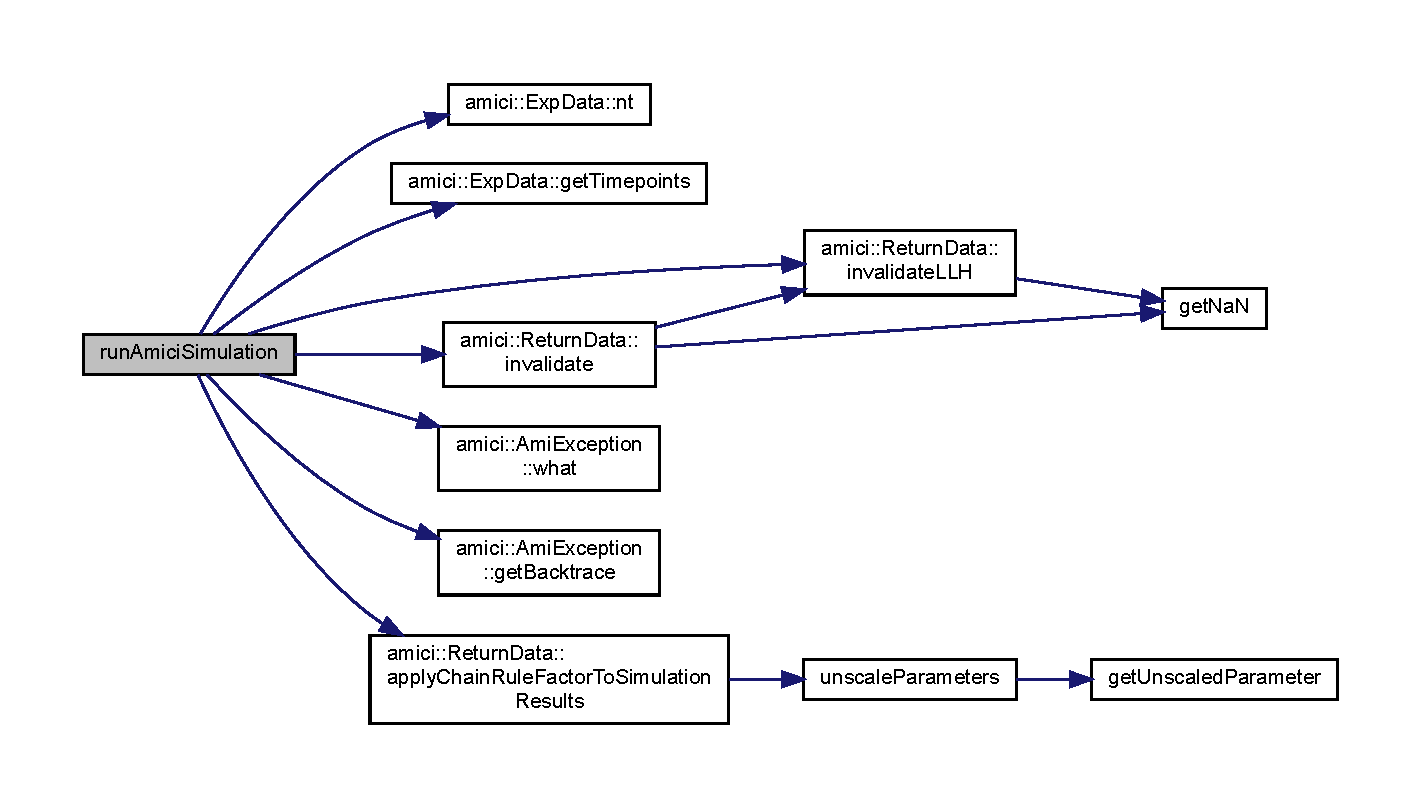
\includegraphics[width=350pt]{namespaceamici_a46331a204e7511587acc2cc0b1ce7ed0_cgraph}
\end{center}
\end{figure}
Here is the caller graph for this function\+:
\nopagebreak
\begin{figure}[H]
\begin{center}
\leavevmode
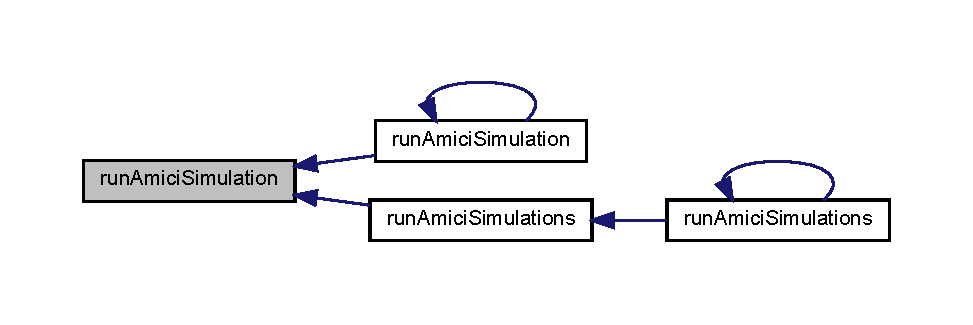
\includegraphics[width=350pt]{namespaceamici_a46331a204e7511587acc2cc0b1ce7ed0_icgraph}
\end{center}
\end{figure}
\mbox{\Hypertarget{namespaceamici_a76e08fb9dd88a6b5352ae53d7afedc1e}\label{namespaceamici_a76e08fb9dd88a6b5352ae53d7afedc1e}} 
\index{amici@{amici}!run\+Amici\+Simulations@{run\+Amici\+Simulations}}
\index{run\+Amici\+Simulations@{run\+Amici\+Simulations}!amici@{amici}}
\paragraph{\texorpdfstring{run\+Amici\+Simulations()}{runAmiciSimulations()}\hspace{0.1cm}{\footnotesize\ttfamily [1/2]}}
{\footnotesize\ttfamily std\+::vector$<$ std\+::unique\+\_\+ptr$<$ \mbox{\hyperlink{classamici_1_1_return_data}{Return\+Data}} $>$ $>$ run\+Amici\+Simulations (\begin{DoxyParamCaption}\item[{\mbox{\hyperlink{classamici_1_1_solver}{Solver}} const \&}]{solver,  }\item[{const std\+::vector$<$ \mbox{\hyperlink{classamici_1_1_exp_data}{Exp\+Data}} $\ast$$>$ \&}]{edatas,  }\item[{\mbox{\hyperlink{classamici_1_1_model}{Model}} const \&}]{model,  }\item[{int}]{num\+\_\+threads }\end{DoxyParamCaption})}

run\+Amici\+Simulations does the same as run\+Amici\+Simulation, but for multiple \mbox{\hyperlink{classamici_1_1_exp_data}{Exp\+Data}} instances.


\begin{DoxyParams}{Parameters}
{\em solver} & \mbox{\hyperlink{classamici_1_1_solver}{Solver}} instance \\
\hline
{\em edatas} & experimental data objects \\
\hline
{\em model} & model specification object \\
\hline
{\em num\+\_\+threads} & number of threads for parallel execution \\
\hline
\end{DoxyParams}
\begin{DoxyReturn}{Returns}
vector of pointers to return data objects 
\end{DoxyReturn}


Definition at line 146 of file amici.\+cpp.

Here is the call graph for this function\+:
\nopagebreak
\begin{figure}[H]
\begin{center}
\leavevmode
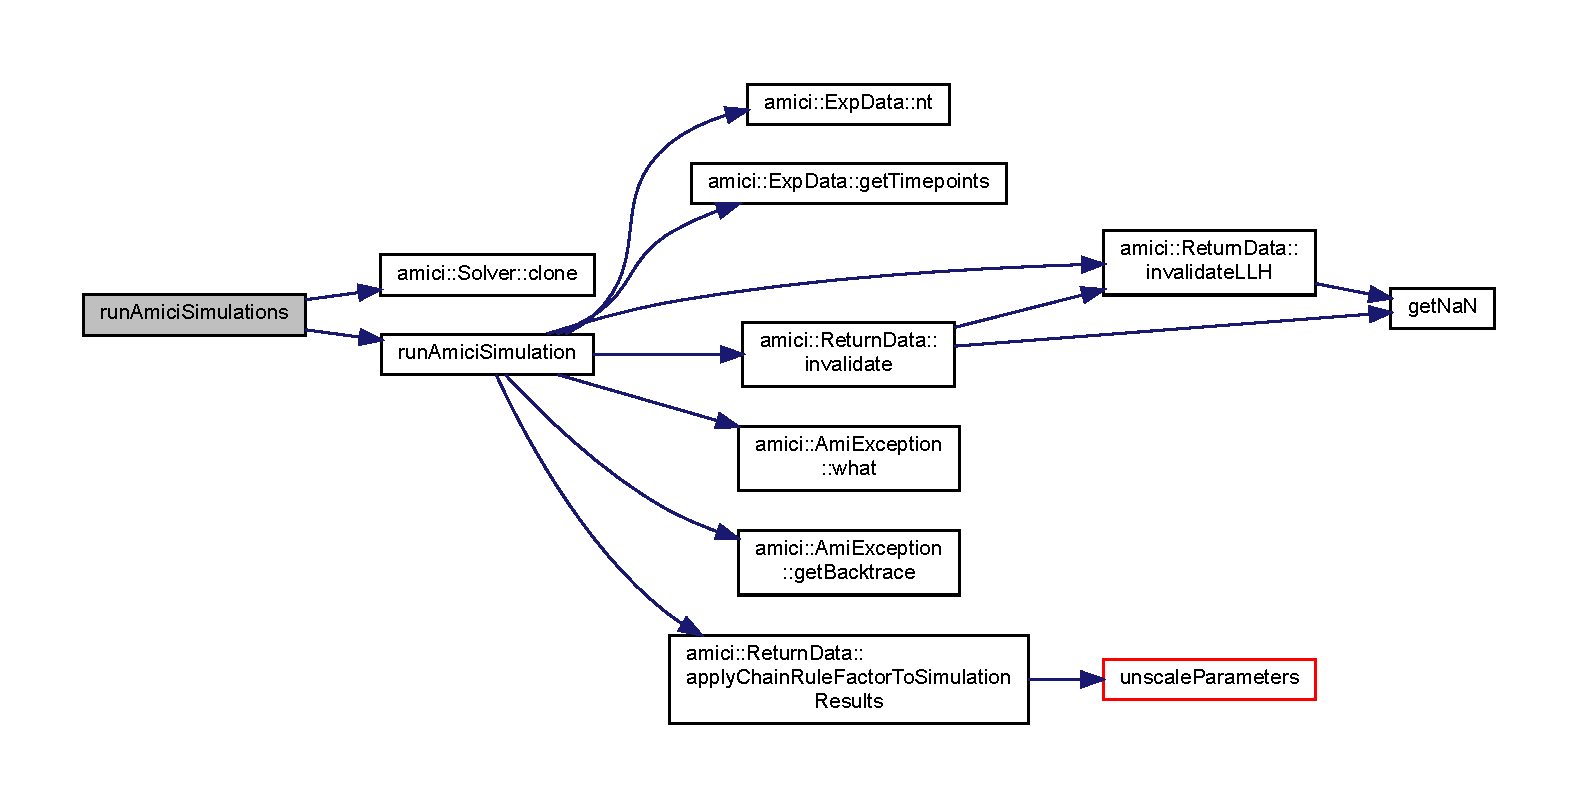
\includegraphics[width=350pt]{namespaceamici_a76e08fb9dd88a6b5352ae53d7afedc1e_cgraph}
\end{center}
\end{figure}
Here is the caller graph for this function\+:
\nopagebreak
\begin{figure}[H]
\begin{center}
\leavevmode
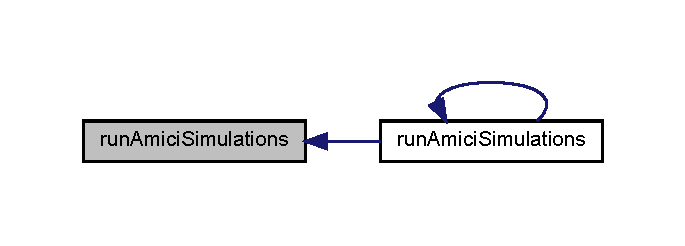
\includegraphics[width=329pt]{namespaceamici_a76e08fb9dd88a6b5352ae53d7afedc1e_icgraph}
\end{center}
\end{figure}
\mbox{\Hypertarget{namespaceamici_aaadff5ccb22e546f3590e15f5ee30c1c}\label{namespaceamici_aaadff5ccb22e546f3590e15f5ee30c1c}} 
\index{amici@{amici}!amici\+\_\+dgemv@{amici\+\_\+dgemv}}
\index{amici\+\_\+dgemv@{amici\+\_\+dgemv}!amici@{amici}}
\paragraph{\texorpdfstring{amici\+\_\+dgemv()}{amici\_dgemv()}}
{\footnotesize\ttfamily void amici\+\_\+dgemv (\begin{DoxyParamCaption}\item[{\mbox{\hyperlink{namespaceamici_a3ec6460bb4e7f6100a15d18627a3ff3e}{B\+L\+A\+S\+Layout}}}]{layout,  }\item[{\mbox{\hyperlink{namespaceamici_a0f0ec77c6c8f48d9c5cb50d54899afae}{B\+L\+A\+S\+Transpose}}}]{TransA,  }\item[{const int}]{M,  }\item[{const int}]{N,  }\item[{const double}]{alpha,  }\item[{const double $\ast$}]{A,  }\item[{const int}]{lda,  }\item[{const double $\ast$}]{X,  }\item[{const int}]{incX,  }\item[{const double}]{beta,  }\item[{double $\ast$}]{Y,  }\item[{const int}]{incY }\end{DoxyParamCaption})}

amici\+\_\+dgemm provides an interface to the blas matrix vector multiplication routine dgemv. This routines computes y = alpha$\ast$\+A$\ast$x + beta$\ast$y with A\+: \mbox{[}MxK\mbox{]} B\+:\mbox{[}KxN\mbox{]} C\+:\mbox{[}MxN\mbox{]}


\begin{DoxyParams}[1]{Parameters}
\mbox{\tt in}  & {\em layout} & can be A\+M\+I\+C\+I\+\_\+\+B\+L\+A\+S\+\_\+\+Col\+Major or A\+M\+I\+C\+I\+\_\+\+B\+L\+A\+S\+\_\+\+Row\+Major. \\
\hline
\mbox{\tt in}  & {\em TransA} & flag indicating whether A should be transposed before multiplication \\
\hline
\mbox{\tt in}  & {\em M} & number of rows in A \\
\hline
\mbox{\tt in}  & {\em N} & number of columns in A \\
\hline
\mbox{\tt in}  & {\em alpha} & coefficient alpha \\
\hline
\mbox{\tt in}  & {\em A} & matrix A \\
\hline
\mbox{\tt in}  & {\em lda} & leading dimension of A (m or n) \\
\hline
\mbox{\tt in}  & {\em X} & vector X \\
\hline
\mbox{\tt in}  & {\em incX} & increment for entries of X \\
\hline
\mbox{\tt in}  & {\em beta} & coefficient beta \\
\hline
\mbox{\tt in,out}  & {\em Y} & vector Y \\
\hline
\mbox{\tt in}  & {\em incY} & increment for entries of Y\\
\hline
\end{DoxyParams}
amici\+\_\+dgemm provides an interface to the C\+Blas matrix vector multiplication routine dgemv. This routines computes y = alpha$\ast$\+A$\ast$x + beta$\ast$y with A\+: \mbox{[}MxN\mbox{]} x\+:\mbox{[}Nx1\mbox{]} y\+:\mbox{[}Mx1\mbox{]}


\begin{DoxyParams}{Parameters}
{\em layout} & always needs to be A\+M\+I\+C\+I\+\_\+\+B\+L\+A\+S\+\_\+\+Col\+Major. \\
\hline
{\em TransA} & flag indicating whether A should be transposed before multiplication \\
\hline
{\em M} & number of rows in A \\
\hline
{\em N} & number of columns in A \\
\hline
{\em alpha} & coefficient alpha \\
\hline
{\em A} & matrix A \\
\hline
{\em lda} & leading dimension of A (m or n) \\
\hline
{\em X} & vector X \\
\hline
{\em incX} & increment for entries of X \\
\hline
{\em beta} & coefficient beta \\
\hline
{\em Y} & vector Y \\
\hline
{\em incY} & increment for entries of Y \\
\hline
\end{DoxyParams}
\begin{DoxyReturn}{Returns}
void 
\end{DoxyReturn}


Definition at line 73 of file cblas.\+cpp.

\mbox{\Hypertarget{namespaceamici_a235c0cbd2185cc7351ea9c126e498bd9}\label{namespaceamici_a235c0cbd2185cc7351ea9c126e498bd9}} 
\index{amici@{amici}!amici\+\_\+dgemm@{amici\+\_\+dgemm}}
\index{amici\+\_\+dgemm@{amici\+\_\+dgemm}!amici@{amici}}
\paragraph{\texorpdfstring{amici\+\_\+dgemm()}{amici\_dgemm()}}
{\footnotesize\ttfamily void amici\+\_\+dgemm (\begin{DoxyParamCaption}\item[{\mbox{\hyperlink{namespaceamici_a3ec6460bb4e7f6100a15d18627a3ff3e}{B\+L\+A\+S\+Layout}}}]{layout,  }\item[{\mbox{\hyperlink{namespaceamici_a0f0ec77c6c8f48d9c5cb50d54899afae}{B\+L\+A\+S\+Transpose}}}]{TransA,  }\item[{\mbox{\hyperlink{namespaceamici_a0f0ec77c6c8f48d9c5cb50d54899afae}{B\+L\+A\+S\+Transpose}}}]{TransB,  }\item[{const int}]{M,  }\item[{const int}]{N,  }\item[{const int}]{K,  }\item[{const double}]{alpha,  }\item[{const double $\ast$}]{A,  }\item[{const int}]{lda,  }\item[{const double $\ast$}]{B,  }\item[{const int}]{ldb,  }\item[{const double}]{beta,  }\item[{double $\ast$}]{C,  }\item[{const int}]{ldc }\end{DoxyParamCaption})}

amici\+\_\+dgemm provides an interface to the blas matrix matrix multiplication routine dgemm. This routines computes C = alpha$\ast$\+A$\ast$B + beta$\ast$C with A\+: \mbox{[}MxK\mbox{]} B\+:\mbox{[}KxN\mbox{]} C\+:\mbox{[}MxN\mbox{]}


\begin{DoxyParams}[1]{Parameters}
\mbox{\tt in}  & {\em layout} & can be A\+M\+I\+C\+I\+\_\+\+B\+L\+A\+S\+\_\+\+Col\+Major or A\+M\+I\+C\+I\+\_\+\+B\+L\+A\+S\+\_\+\+Row\+Major. \\
\hline
\mbox{\tt in}  & {\em TransA} & flag indicating whether A should be transposed before multiplication \\
\hline
\mbox{\tt in}  & {\em TransB} & flag indicating whether B should be transposed before multiplication \\
\hline
\mbox{\tt in}  & {\em M} & number of rows in A/C \\
\hline
\mbox{\tt in}  & {\em N} & number of columns in B/C \\
\hline
\mbox{\tt in}  & {\em K} & number of rows in B, number of columns in A \\
\hline
\mbox{\tt in}  & {\em alpha} & coefficient alpha \\
\hline
\mbox{\tt in}  & {\em A} & matrix A \\
\hline
\mbox{\tt in}  & {\em lda} & leading dimension of A (m or k) \\
\hline
\mbox{\tt in}  & {\em B} & matrix B \\
\hline
\mbox{\tt in}  & {\em ldb} & leading dimension of B (k or n) \\
\hline
\mbox{\tt in}  & {\em beta} & coefficient beta \\
\hline
\mbox{\tt in,out}  & {\em C} & matrix C \\
\hline
\mbox{\tt in}  & {\em ldc} & leading dimension of C (m or n)\\
\hline
\end{DoxyParams}
amici\+\_\+dgemm provides an interface to the C\+Blas matrix matrix multiplication routine dgemm. This routines computes C = alpha$\ast$\+A$\ast$B + beta$\ast$C with A\+: \mbox{[}MxK\mbox{]} B\+:\mbox{[}KxN\mbox{]} C\+:\mbox{[}MxN\mbox{]}


\begin{DoxyParams}{Parameters}
{\em layout} & memory layout. \\
\hline
{\em TransA} & flag indicating whether A should be transposed before multiplication \\
\hline
{\em TransB} & flag indicating whether B should be transposed before multiplication \\
\hline
{\em M} & number of rows in A/C \\
\hline
{\em N} & number of columns in B/C \\
\hline
{\em K} & number of rows in B, number of columns in A \\
\hline
{\em alpha} & coefficient alpha \\
\hline
{\em A} & matrix A \\
\hline
{\em lda} & leading dimension of A (m or k) \\
\hline
{\em B} & matrix B \\
\hline
{\em ldb} & leading dimension of B (k or n) \\
\hline
{\em beta} & coefficient beta \\
\hline
{\em C} & matrix C \\
\hline
{\em ldc} & leading dimension of C (m or n) \\
\hline
\end{DoxyParams}
\begin{DoxyReturn}{Returns}
void 
\end{DoxyReturn}


Definition at line 44 of file cblas.\+cpp.

Here is the caller graph for this function\+:
\nopagebreak
\begin{figure}[H]
\begin{center}
\leavevmode
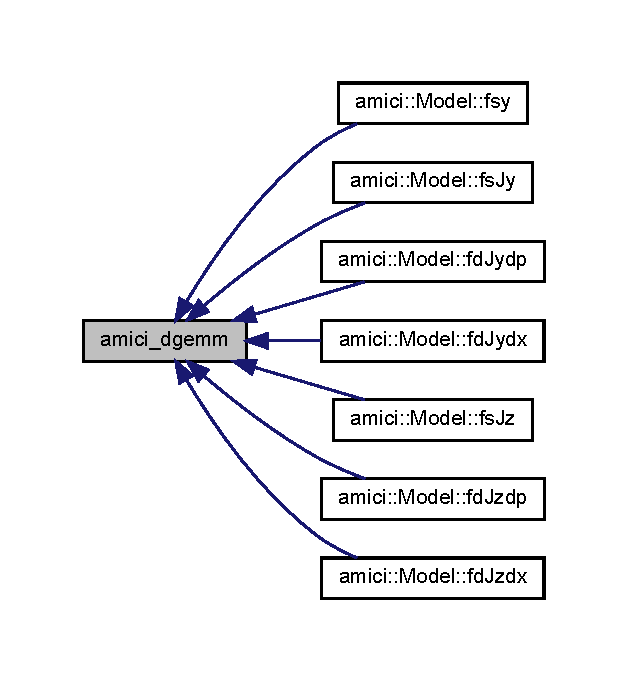
\includegraphics[width=301pt]{namespaceamici_a235c0cbd2185cc7351ea9c126e498bd9_icgraph}
\end{center}
\end{figure}
\mbox{\Hypertarget{namespaceamici_ad4c586891a96a47c0a73f8585d6aabcf}\label{namespaceamici_ad4c586891a96a47c0a73f8585d6aabcf}} 
\index{amici@{amici}!amici\+\_\+daxpy@{amici\+\_\+daxpy}}
\index{amici\+\_\+daxpy@{amici\+\_\+daxpy}!amici@{amici}}
\paragraph{\texorpdfstring{amici\+\_\+daxpy()}{amici\_daxpy()}}
{\footnotesize\ttfamily void amici\+\_\+daxpy (\begin{DoxyParamCaption}\item[{int}]{n,  }\item[{double}]{alpha,  }\item[{const double $\ast$}]{x,  }\item[{const int}]{incx,  }\item[{double $\ast$}]{y,  }\item[{int}]{incy }\end{DoxyParamCaption})}


\begin{DoxyParams}{Parameters}
{\em n} & number of elements in y \\
\hline
{\em alpha} & scalar coefficient of x \\
\hline
{\em x} & vector of length n$\ast$incx \\
\hline
{\em incx} & x stride \\
\hline
{\em y} & vector of length n$\ast$incy \\
\hline
{\em incy} & y stride \\
\hline
\end{DoxyParams}


Definition at line 90 of file cblas.\+cpp.

\mbox{\Hypertarget{namespaceamici_aacdc2fc7895f234ad13713d2bd99870d}\label{namespaceamici_aacdc2fc7895f234ad13713d2bd99870d}} 
\index{amici@{amici}!set\+Model\+Data@{set\+Model\+Data}}
\index{set\+Model\+Data@{set\+Model\+Data}!amici@{amici}}
\paragraph{\texorpdfstring{set\+Model\+Data()}{setModelData()}}
{\footnotesize\ttfamily void set\+Model\+Data (\begin{DoxyParamCaption}\item[{const mx\+Array $\ast$}]{prhs\mbox{[}$\,$\mbox{]},  }\item[{int}]{nrhs,  }\item[{\mbox{\hyperlink{classamici_1_1_model}{Model}} \&}]{model }\end{DoxyParamCaption})}


\begin{DoxyParams}[1]{Parameters}
\mbox{\tt in}  & {\em prhs} & pointer to the array of input arguments ~\newline
{\bfseries Type}\+: mx\+Array \\
\hline
\mbox{\tt in}  & {\em nrhs} & number of elements in prhs \\
\hline
\mbox{\tt in,out}  & {\em model} & model to update \\
\hline
\end{DoxyParams}


Definition at line 389 of file interface\+\_\+matlab.\+cpp.

Here is the call graph for this function\+:
\nopagebreak
\begin{figure}[H]
\begin{center}
\leavevmode
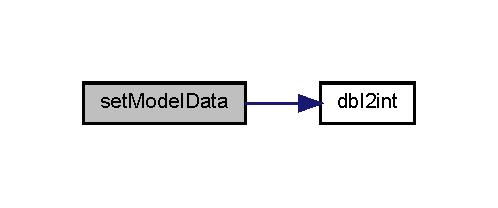
\includegraphics[width=239pt]{namespaceamici_aacdc2fc7895f234ad13713d2bd99870d_cgraph}
\end{center}
\end{figure}
\mbox{\Hypertarget{namespaceamici_aab6be0027d918715e2ba50828088110b}\label{namespaceamici_aab6be0027d918715e2ba50828088110b}} 
\index{amici@{amici}!set\+Solver\+Options@{set\+Solver\+Options}}
\index{set\+Solver\+Options@{set\+Solver\+Options}!amici@{amici}}
\paragraph{\texorpdfstring{set\+Solver\+Options()}{setSolverOptions()}}
{\footnotesize\ttfamily void set\+Solver\+Options (\begin{DoxyParamCaption}\item[{const mx\+Array $\ast$}]{prhs\mbox{[}$\,$\mbox{]},  }\item[{int}]{nrhs,  }\item[{\mbox{\hyperlink{classamici_1_1_solver}{Solver}} \&}]{solver }\end{DoxyParamCaption})}


\begin{DoxyParams}[1]{Parameters}
\mbox{\tt in}  & {\em prhs} & pointer to the array of input arguments ~\newline
{\bfseries Type}\+: mx\+Array \\
\hline
\mbox{\tt in}  & {\em nrhs} & number of elements in prhs \\
\hline
\mbox{\tt in,out}  & {\em solver} & solver to update \\
\hline
\end{DoxyParams}


Definition at line 304 of file interface\+\_\+matlab.\+cpp.

Here is the call graph for this function\+:
\nopagebreak
\begin{figure}[H]
\begin{center}
\leavevmode
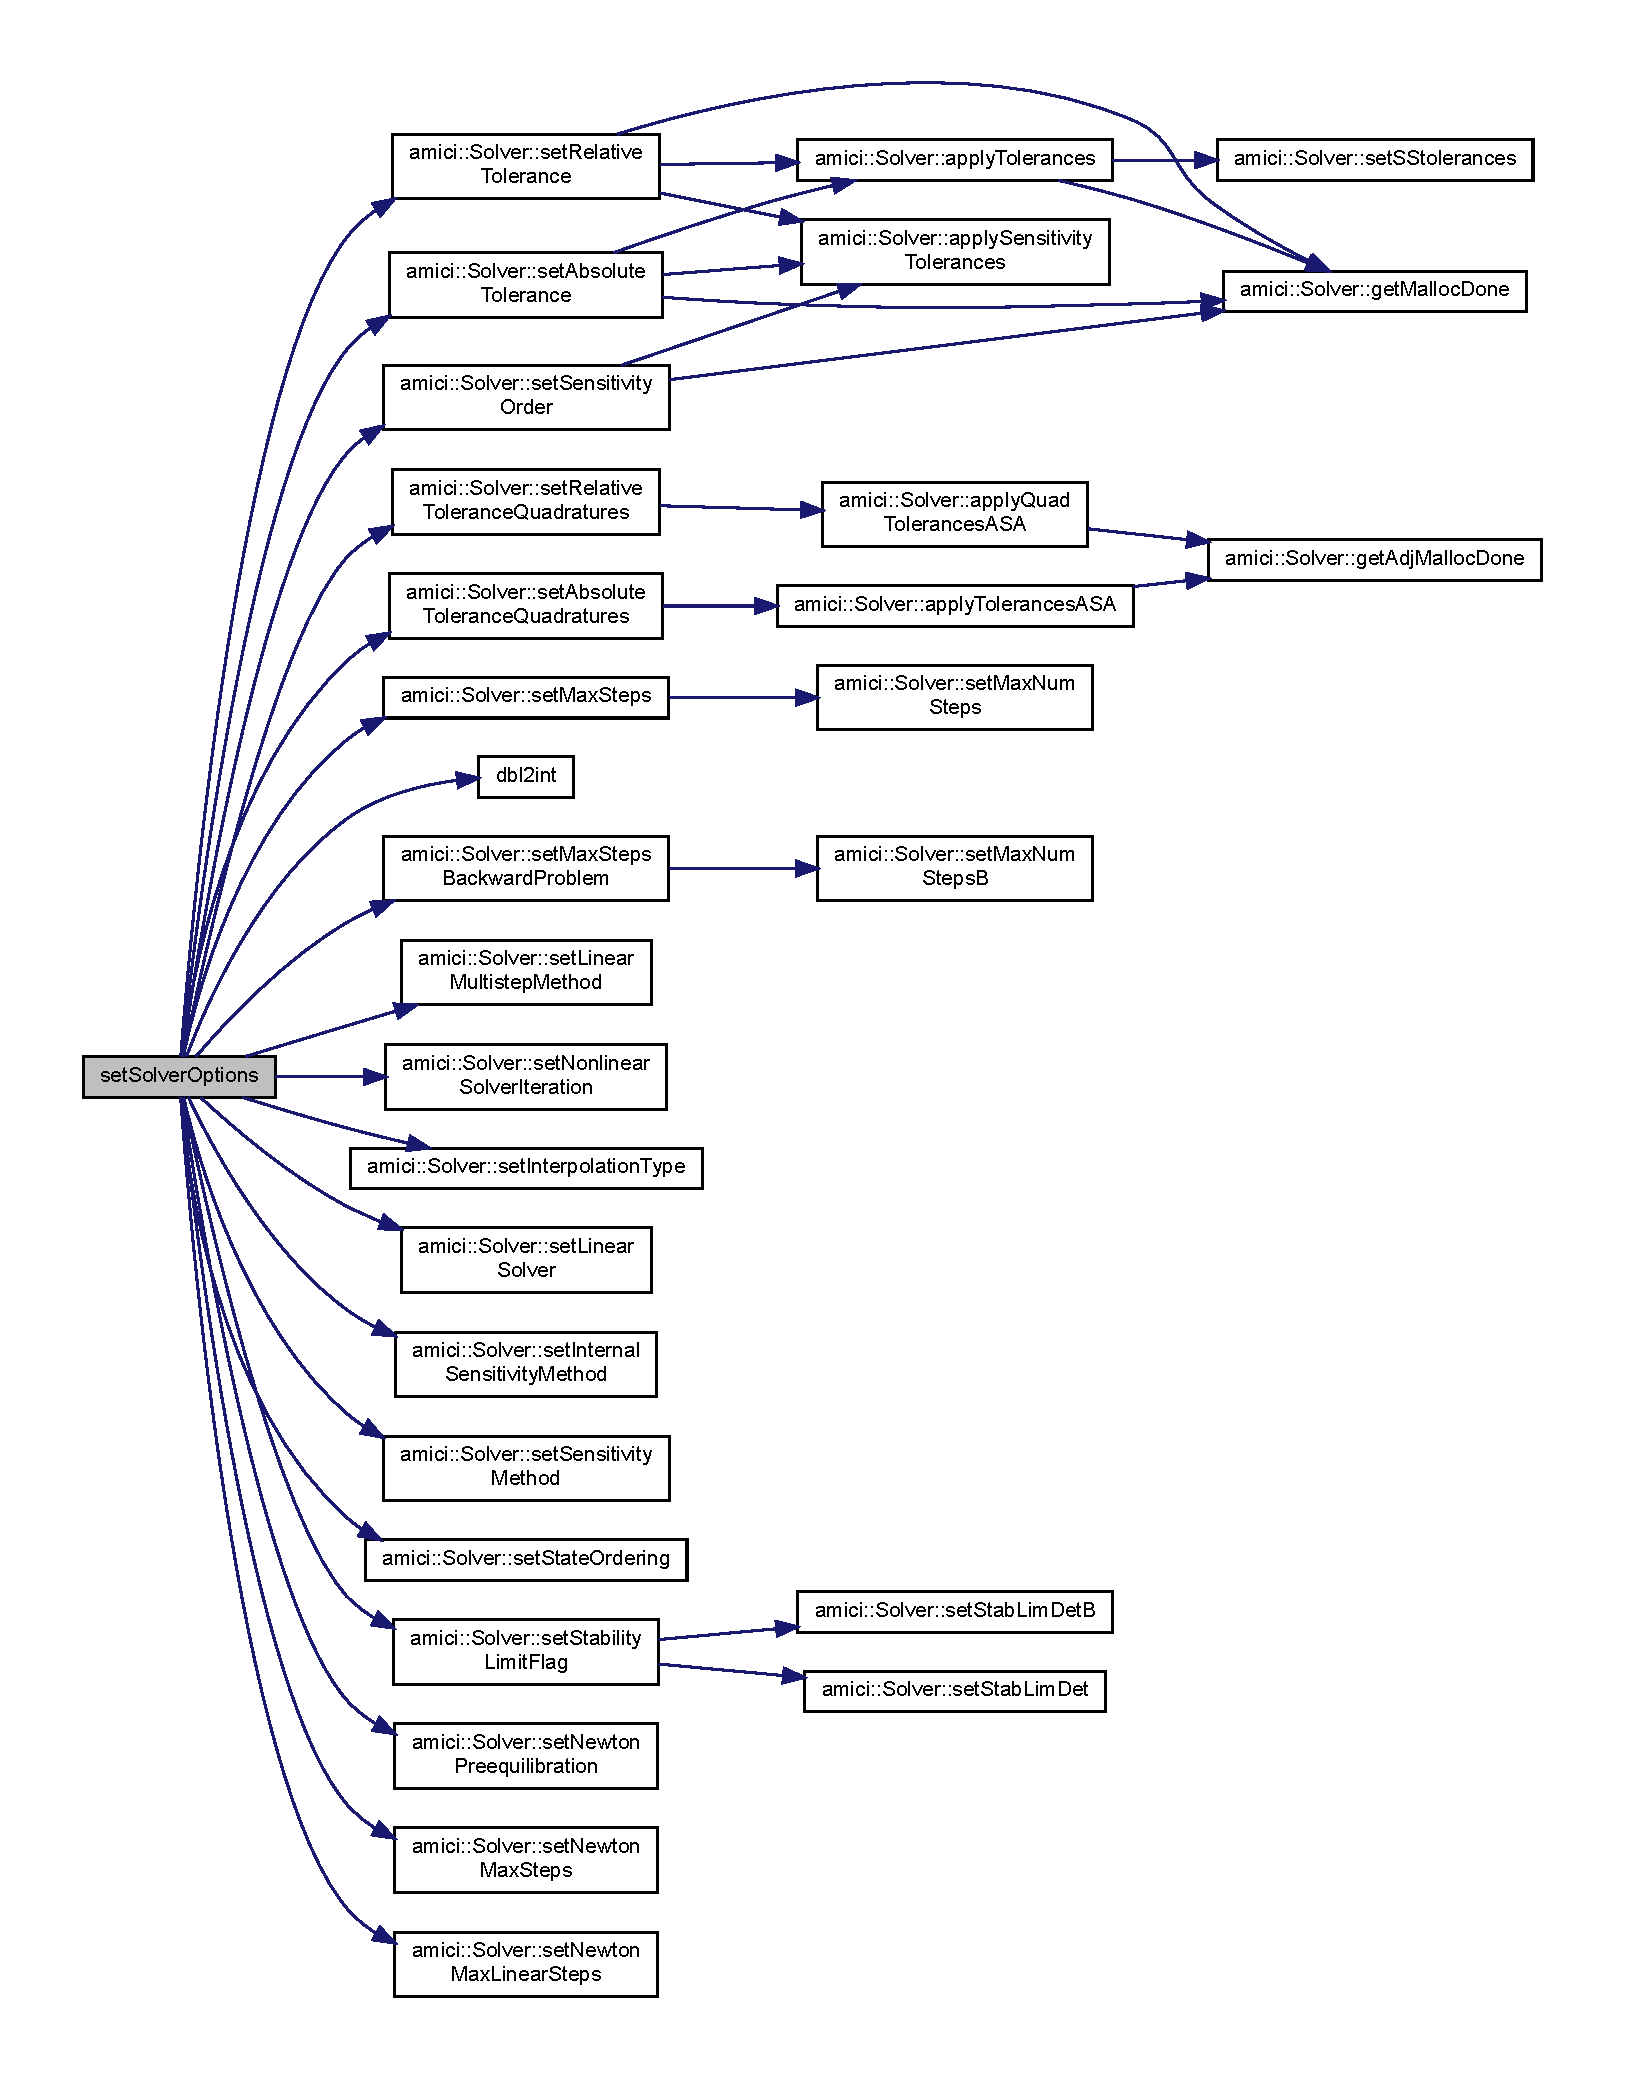
\includegraphics[width=350pt]{namespaceamici_aab6be0027d918715e2ba50828088110b_cgraph}
\end{center}
\end{figure}
\mbox{\Hypertarget{namespaceamici_a91a3ac85998f7dd60d633882e9504b07}\label{namespaceamici_a91a3ac85998f7dd60d633882e9504b07}} 
\index{amici@{amici}!setup\+Return\+Data@{setup\+Return\+Data}}
\index{setup\+Return\+Data@{setup\+Return\+Data}!amici@{amici}}
\paragraph{\texorpdfstring{setup\+Return\+Data()}{setupReturnData()}}
{\footnotesize\ttfamily Return\+Data\+Matlab$\ast$ amici\+::setup\+Return\+Data (\begin{DoxyParamCaption}\item[{mx\+Array $\ast$}]{plhs\mbox{[}$\,$\mbox{]},  }\item[{int}]{nlhs }\end{DoxyParamCaption})}

setup\+Return\+Data initialises the return data struct 
\begin{DoxyParams}[1]{Parameters}
\mbox{\tt in}  & {\em plhs} & user input ~\newline
{\bfseries Type}\+: mx\+Array \\
\hline
\mbox{\tt in}  & {\em nlhs} & number of elements in plhs ~\newline
{\bfseries Type}\+: mx\+Array \\
\hline
\end{DoxyParams}
\begin{DoxyReturn}{Returns}
rdata\+: return data struct ~\newline
{\bfseries Type}\+: $\ast$\+Return\+Data 
\end{DoxyReturn}
\mbox{\Hypertarget{namespaceamici_a186dd3debfe185669f305464f161e4bb}\label{namespaceamici_a186dd3debfe185669f305464f161e4bb}} 
\index{amici@{amici}!exp\+Data\+From\+Matlab\+Call@{exp\+Data\+From\+Matlab\+Call}}
\index{exp\+Data\+From\+Matlab\+Call@{exp\+Data\+From\+Matlab\+Call}!amici@{amici}}
\paragraph{\texorpdfstring{exp\+Data\+From\+Matlab\+Call()}{expDataFromMatlabCall()}}
{\footnotesize\ttfamily std\+::unique\+\_\+ptr$<$ \mbox{\hyperlink{classamici_1_1_exp_data}{Exp\+Data}} $>$ exp\+Data\+From\+Matlab\+Call (\begin{DoxyParamCaption}\item[{const mx\+Array $\ast$}]{prhs\mbox{[}$\,$\mbox{]},  }\item[{const \mbox{\hyperlink{classamici_1_1_model}{Model}} \&}]{model }\end{DoxyParamCaption})}

exp\+Data\+From\+Matlab\+Call initialises the experimental data struct 
\begin{DoxyParams}[1]{Parameters}
\mbox{\tt in}  & {\em prhs} & user input ~\newline
{\bfseries Type}\+: $\ast$mx\+Array \\
\hline
\end{DoxyParams}
\begin{DoxyReturn}{Returns}
edata\+: experimental data struct ~\newline
{\bfseries Type}\+: $\ast$\+Exp\+Data
\end{DoxyReturn}
exp\+Data\+From\+Matlab\+Call parses the experimental data from the matlab call and writes it to an \mbox{\hyperlink{classamici_1_1_exp_data}{Exp\+Data}} class object


\begin{DoxyParams}{Parameters}
{\em prhs} & pointer to the array of input arguments \\
\hline
{\em model} & pointer to the model object, this is necessary to perform dimension checks \\
\hline
\end{DoxyParams}
\begin{DoxyReturn}{Returns}
edata pointer to experimental data object 
\end{DoxyReturn}


Definition at line 179 of file interface\+\_\+matlab.\+cpp.

Here is the call graph for this function\+:
\nopagebreak
\begin{figure}[H]
\begin{center}
\leavevmode
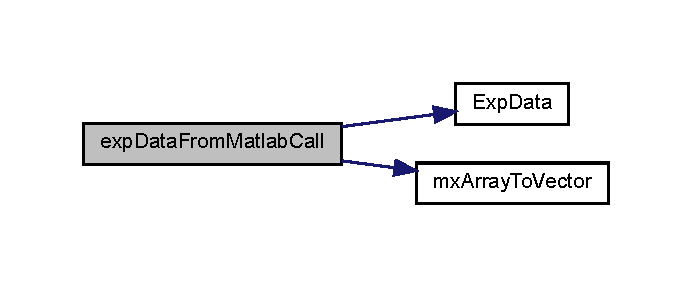
\includegraphics[width=332pt]{namespaceamici_a186dd3debfe185669f305464f161e4bb_cgraph}
\end{center}
\end{figure}
Here is the caller graph for this function\+:
\nopagebreak
\begin{figure}[H]
\begin{center}
\leavevmode
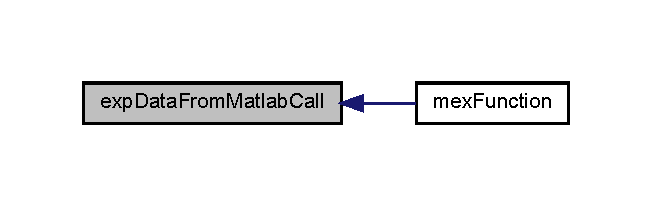
\includegraphics[width=313pt]{namespaceamici_a186dd3debfe185669f305464f161e4bb_icgraph}
\end{center}
\end{figure}
\mbox{\Hypertarget{namespaceamici_aeb0886d5a74ea04eeef52219063aa7d4}\label{namespaceamici_aeb0886d5a74ea04eeef52219063aa7d4}} 
\index{amici@{amici}!check\+Finite@{check\+Finite}}
\index{check\+Finite@{check\+Finite}!amici@{amici}}
\paragraph{\texorpdfstring{check\+Finite()}{checkFinite()}}
{\footnotesize\ttfamily int check\+Finite (\begin{DoxyParamCaption}\item[{const int}]{N,  }\item[{const \mbox{\hyperlink{namespaceamici_a1bdce28051d6a53868f7ccbf5f2c14a3}{realtype}} $\ast$}]{array,  }\item[{const char $\ast$}]{fun }\end{DoxyParamCaption})}

Checks the values in an array for Na\+Ns and Infs


\begin{DoxyParams}{Parameters}
{\em N} & number of elements in array \\
\hline
{\em array} & array \\
\hline
{\em fun} & name of calling function \\
\hline
\end{DoxyParams}
\begin{DoxyReturn}{Returns}
A\+M\+I\+C\+I\+\_\+\+R\+E\+C\+O\+V\+E\+R\+A\+B\+L\+E\+\_\+\+E\+R\+R\+OR if a Na\+N/\+Inf value was found, A\+M\+I\+C\+I\+\_\+\+S\+U\+C\+C\+E\+SS otherwise 
\end{DoxyReturn}


Definition at line 17 of file misc.\+cpp.

Here is the call graph for this function\+:
\nopagebreak
\begin{figure}[H]
\begin{center}
\leavevmode
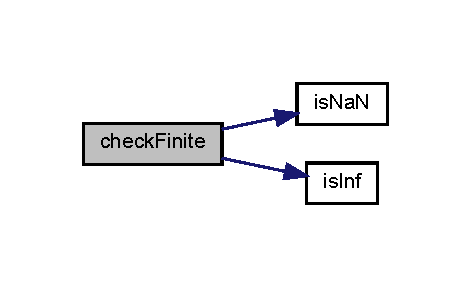
\includegraphics[width=226pt]{namespaceamici_aeb0886d5a74ea04eeef52219063aa7d4_cgraph}
\end{center}
\end{figure}
Here is the caller graph for this function\+:
\nopagebreak
\begin{figure}[H]
\begin{center}
\leavevmode
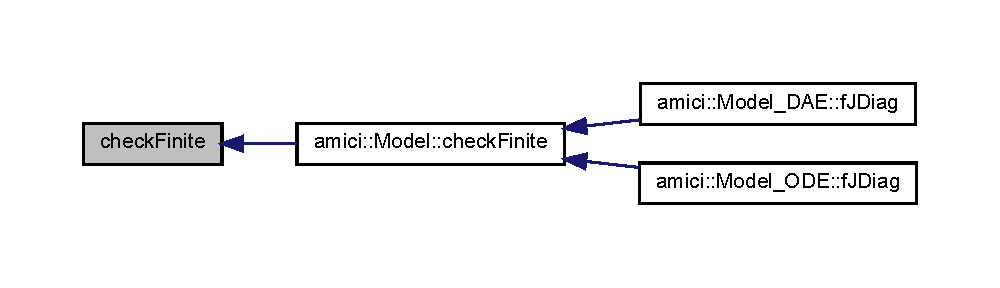
\includegraphics[width=350pt]{namespaceamici_aeb0886d5a74ea04eeef52219063aa7d4_icgraph}
\end{center}
\end{figure}
\mbox{\Hypertarget{namespaceamici_af7d0af67f181a659c78b7aa2bbaaf718}\label{namespaceamici_af7d0af67f181a659c78b7aa2bbaaf718}} 
\index{amici@{amici}!unscale\+Parameters@{unscale\+Parameters}}
\index{unscale\+Parameters@{unscale\+Parameters}!amici@{amici}}
\paragraph{\texorpdfstring{unscale\+Parameters()}{unscaleParameters()}\hspace{0.1cm}{\footnotesize\ttfamily [1/2]}}
{\footnotesize\ttfamily void unscale\+Parameters (\begin{DoxyParamCaption}\item[{const double $\ast$}]{buffer\+Scaled,  }\item[{const \mbox{\hyperlink{namespaceamici_a42f062082226e9284c201d9eab71a3a0}{Parameter\+Scaling}} $\ast$}]{pscale,  }\item[{int}]{n,  }\item[{double $\ast$}]{buffer\+Unscaled }\end{DoxyParamCaption})}


\begin{DoxyParams}{Parameters}
{\em buffer\+Scaled} & scaled parameters \\
\hline
{\em pscale} & parameter scaling \\
\hline
{\em n} & number of elements in buffer\+Scaled, pscale and buffer\+Unscaled \\
\hline
{\em buffer\+Unscaled} & unscaled parameters are written to the array\\
\hline
\end{DoxyParams}
\begin{DoxyReturn}{Returns}
status flag indicating success of execution ~\newline
{\bfseries Type}\+: int 
\end{DoxyReturn}


Definition at line 46 of file misc.\+cpp.

Here is the call graph for this function\+:
\nopagebreak
\begin{figure}[H]
\begin{center}
\leavevmode
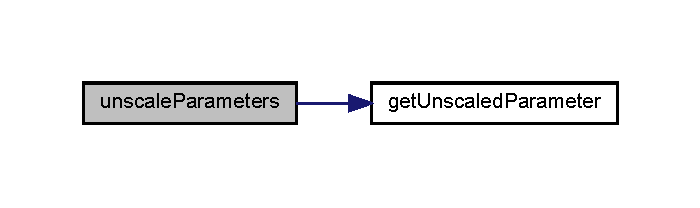
\includegraphics[width=336pt]{namespaceamici_af7d0af67f181a659c78b7aa2bbaaf718_cgraph}
\end{center}
\end{figure}
Here is the caller graph for this function\+:
\nopagebreak
\begin{figure}[H]
\begin{center}
\leavevmode
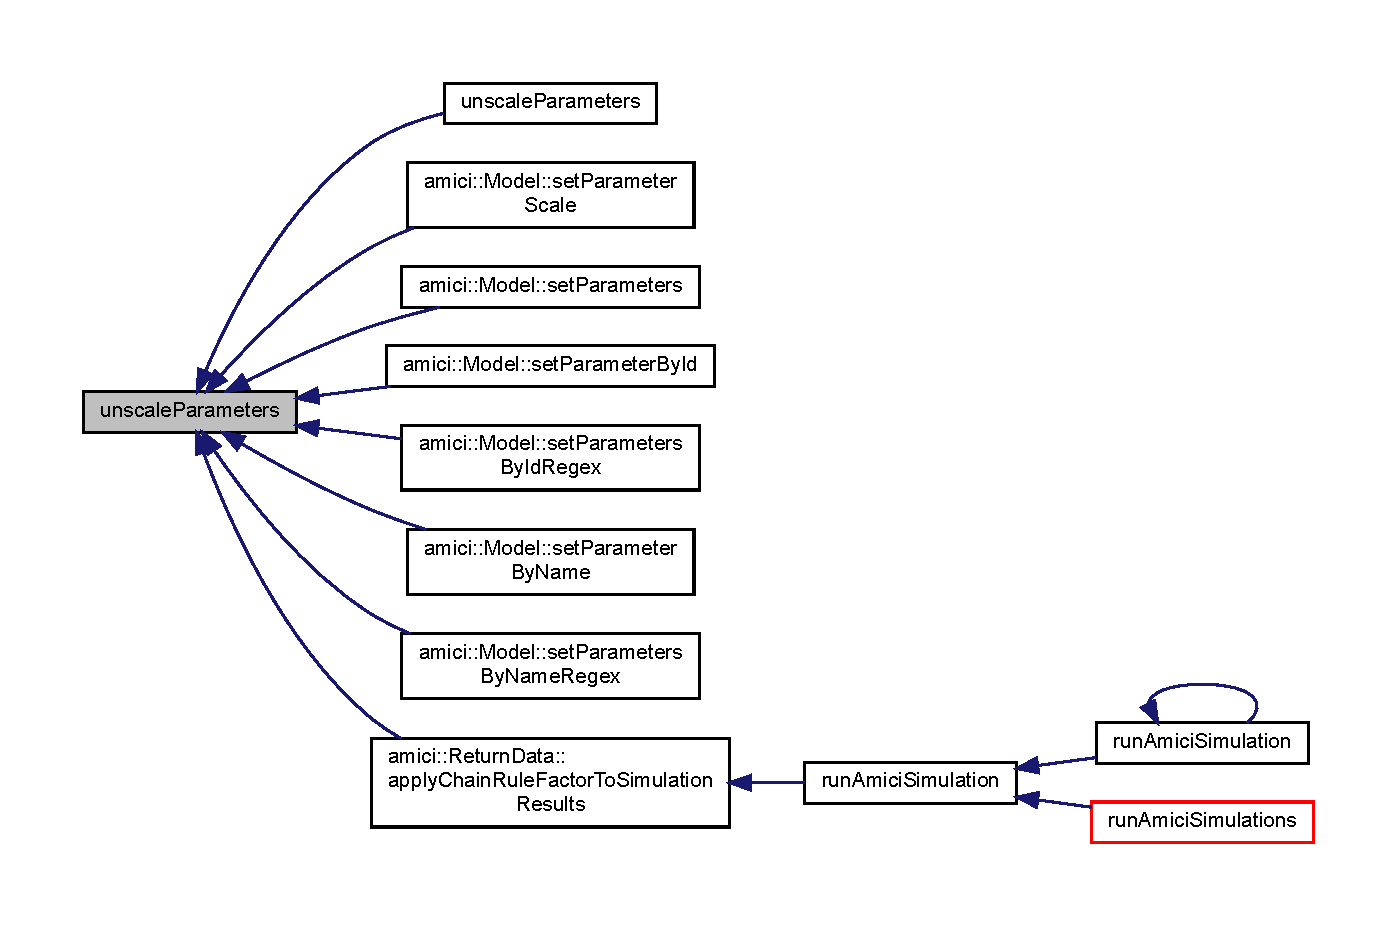
\includegraphics[width=350pt]{namespaceamici_af7d0af67f181a659c78b7aa2bbaaf718_icgraph}
\end{center}
\end{figure}
\mbox{\Hypertarget{namespaceamici_a431c1153fbdccf5ab726863030bc2701}\label{namespaceamici_a431c1153fbdccf5ab726863030bc2701}} 
\index{amici@{amici}!unscale\+Parameters@{unscale\+Parameters}}
\index{unscale\+Parameters@{unscale\+Parameters}!amici@{amici}}
\paragraph{\texorpdfstring{unscale\+Parameters()}{unscaleParameters()}\hspace{0.1cm}{\footnotesize\ttfamily [2/2]}}
{\footnotesize\ttfamily void unscale\+Parameters (\begin{DoxyParamCaption}\item[{std\+::vector$<$ double $>$ const \&}]{buffer\+Scaled,  }\item[{std\+::vector$<$ \mbox{\hyperlink{namespaceamici_a42f062082226e9284c201d9eab71a3a0}{Parameter\+Scaling}} $>$ const \&}]{pscale,  }\item[{std\+::vector$<$ double $>$ \&}]{buffer\+Unscaled }\end{DoxyParamCaption})}

All vectors must be of same length


\begin{DoxyParams}{Parameters}
{\em buffer\+Scaled} & scaled parameters \\
\hline
{\em pscale} & parameter scaling \\
\hline
{\em buffer\+Unscaled} & unscaled parameters are written to the array\\
\hline
\end{DoxyParams}
\begin{DoxyReturn}{Returns}
status flag indicating success of execution ~\newline
{\bfseries Type}\+: int 
\end{DoxyReturn}


Definition at line 54 of file misc.\+cpp.

Here is the call graph for this function\+:
\nopagebreak
\begin{figure}[H]
\begin{center}
\leavevmode
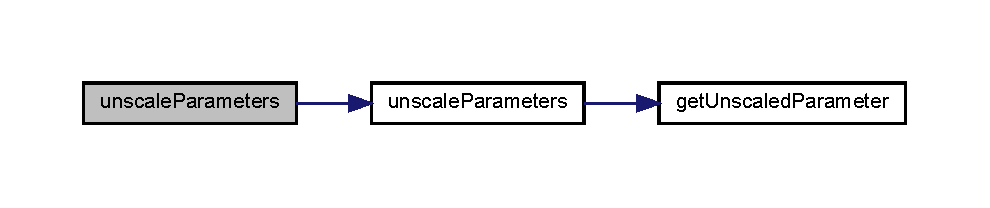
\includegraphics[width=350pt]{namespaceamici_a431c1153fbdccf5ab726863030bc2701_cgraph}
\end{center}
\end{figure}
\mbox{\Hypertarget{namespaceamici_a7e1720941869974da1ca8dbd6cd9e936}\label{namespaceamici_a7e1720941869974da1ca8dbd6cd9e936}} 
\index{amici@{amici}!get\+Unscaled\+Parameter@{get\+Unscaled\+Parameter}}
\index{get\+Unscaled\+Parameter@{get\+Unscaled\+Parameter}!amici@{amici}}
\paragraph{\texorpdfstring{get\+Unscaled\+Parameter()}{getUnscaledParameter()}}
{\footnotesize\ttfamily double get\+Unscaled\+Parameter (\begin{DoxyParamCaption}\item[{double}]{scaled\+Parameter,  }\item[{\mbox{\hyperlink{namespaceamici_a42f062082226e9284c201d9eab71a3a0}{Parameter\+Scaling}}}]{scaling }\end{DoxyParamCaption})}


\begin{DoxyParams}{Parameters}
{\em scaled\+Parameter} & scaled parameter \\
\hline
{\em scaling} & parameter scaling\\
\hline
\end{DoxyParams}
\begin{DoxyReturn}{Returns}
Unscaled parameter 
\end{DoxyReturn}


Definition at line 32 of file misc.\+cpp.

Here is the caller graph for this function\+:
\nopagebreak
\begin{figure}[H]
\begin{center}
\leavevmode
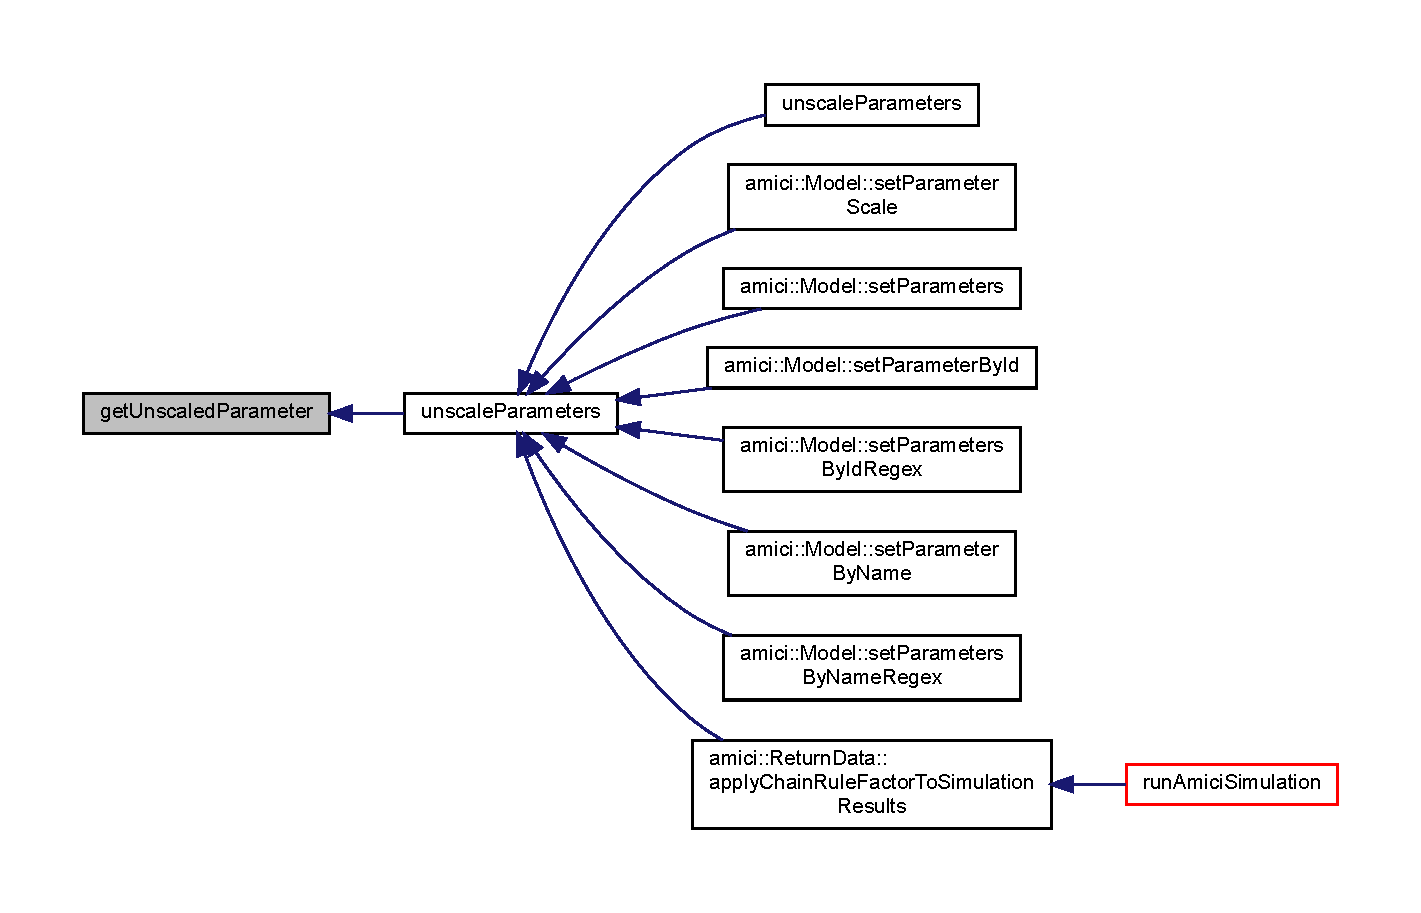
\includegraphics[width=350pt]{namespaceamici_a7e1720941869974da1ca8dbd6cd9e936_icgraph}
\end{center}
\end{figure}
\mbox{\Hypertarget{namespaceamici_ad5a9ae5abc63d6c24c64506c0f9aed6d}\label{namespaceamici_ad5a9ae5abc63d6c24c64506c0f9aed6d}} 
\index{amici@{amici}!operator==@{operator==}}
\index{operator==@{operator==}!amici@{amici}}
\paragraph{\texorpdfstring{operator==()}{operator==()}\hspace{0.1cm}{\footnotesize\ttfamily [1/2]}}
{\footnotesize\ttfamily bool operator== (\begin{DoxyParamCaption}\item[{const \mbox{\hyperlink{classamici_1_1_model}{Model}} \&}]{a,  }\item[{const \mbox{\hyperlink{classamici_1_1_model}{Model}} \&}]{b }\end{DoxyParamCaption})}


\begin{DoxyParams}{Parameters}
{\em a} & first model instance \\
\hline
{\em b} & second model instance \\
\hline
\end{DoxyParams}
\begin{DoxyReturn}{Returns}
equality 
\end{DoxyReturn}


Definition at line 1297 of file model.\+cpp.

\mbox{\Hypertarget{namespaceamici_a698409f4b9ce06055bcebcee39f81a91}\label{namespaceamici_a698409f4b9ce06055bcebcee39f81a91}} 
\index{amici@{amici}!get\+Return\+Data\+Matlab\+From\+Amici\+Call@{get\+Return\+Data\+Matlab\+From\+Amici\+Call}}
\index{get\+Return\+Data\+Matlab\+From\+Amici\+Call@{get\+Return\+Data\+Matlab\+From\+Amici\+Call}!amici@{amici}}
\paragraph{\texorpdfstring{get\+Return\+Data\+Matlab\+From\+Amici\+Call()}{getReturnDataMatlabFromAmiciCall()}}
{\footnotesize\ttfamily mx\+Array $\ast$ get\+Return\+Data\+Matlab\+From\+Amici\+Call (\begin{DoxyParamCaption}\item[{\mbox{\hyperlink{classamici_1_1_return_data}{Return\+Data}} const $\ast$}]{rdata }\end{DoxyParamCaption})}

generates matlab mx\+Array from a \mbox{\hyperlink{classamici_1_1_return_data}{Return\+Data}} object 
\begin{DoxyParams}{Parameters}
{\em rdata} & Return\+Data\+Object \\
\hline
\end{DoxyParams}
\begin{DoxyReturn}{Returns}
rdatamatlab Return\+Data\+Object stored as matlab compatible data
\end{DoxyReturn}
generates matlab mx\+Array from a \mbox{\hyperlink{classamici_1_1_return_data}{Return\+Data}} object 
\begin{DoxyParams}{Parameters}
{\em rdata} & Return\+Data\+Object \\
\hline
\end{DoxyParams}
\begin{DoxyReturn}{Returns}
rdatamatlab Return\+Data\+Object stored as matlab compatible data
\end{DoxyReturn}


Definition at line 7 of file returndata\+\_\+matlab.\+cpp.

Here is the call graph for this function\+:
\nopagebreak
\begin{figure}[H]
\begin{center}
\leavevmode
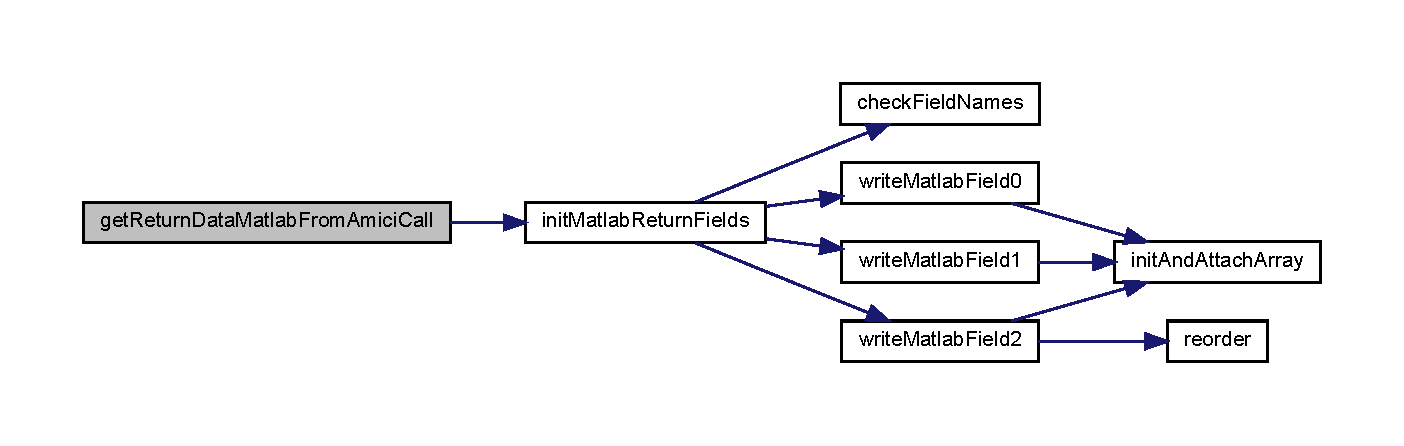
\includegraphics[width=350pt]{namespaceamici_a698409f4b9ce06055bcebcee39f81a91_cgraph}
\end{center}
\end{figure}
\mbox{\Hypertarget{namespaceamici_a7449834fca1e0bde53d5f73ae0d2b929}\label{namespaceamici_a7449834fca1e0bde53d5f73ae0d2b929}} 
\index{amici@{amici}!init\+Matlab\+Return\+Fields@{init\+Matlab\+Return\+Fields}}
\index{init\+Matlab\+Return\+Fields@{init\+Matlab\+Return\+Fields}!amici@{amici}}
\paragraph{\texorpdfstring{init\+Matlab\+Return\+Fields()}{initMatlabReturnFields()}}
{\footnotesize\ttfamily mx\+Array $\ast$ init\+Matlab\+Return\+Fields (\begin{DoxyParamCaption}\item[{\mbox{\hyperlink{classamici_1_1_return_data}{Return\+Data}} const $\ast$}]{rdata }\end{DoxyParamCaption})}

allocates and initialises solution mx\+Array with the corresponding fields


\begin{DoxyParams}{Parameters}
{\em rdata} & Return\+Data\+Object\\
\hline
\end{DoxyParams}
\begin{DoxyReturn}{Returns}
Solution mx\+Array
\end{DoxyReturn}
allocates and initialises solution mx\+Array with the corresponding fields


\begin{DoxyParams}{Parameters}
{\em rdata} & Return\+Data\+Object\\
\hline
\end{DoxyParams}
\begin{DoxyReturn}{Returns}
Solution mx\+Array
\end{DoxyReturn}


Definition at line 18 of file returndata\+\_\+matlab.\+cpp.

Here is the call graph for this function\+:
\nopagebreak
\begin{figure}[H]
\begin{center}
\leavevmode
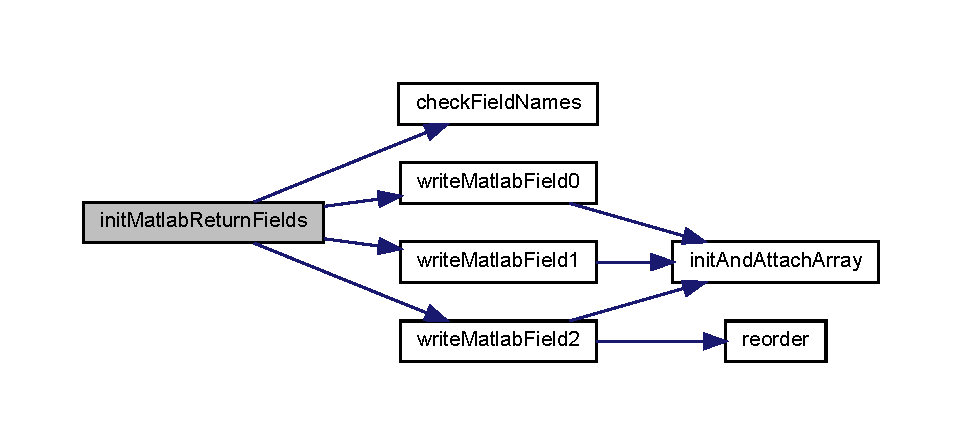
\includegraphics[width=350pt]{namespaceamici_a7449834fca1e0bde53d5f73ae0d2b929_cgraph}
\end{center}
\end{figure}
Here is the caller graph for this function\+:
\nopagebreak
\begin{figure}[H]
\begin{center}
\leavevmode
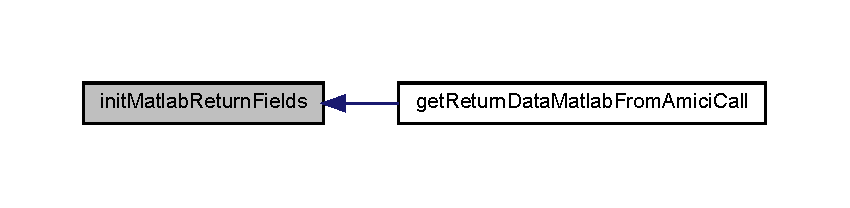
\includegraphics[width=350pt]{namespaceamici_a7449834fca1e0bde53d5f73ae0d2b929_icgraph}
\end{center}
\end{figure}
\mbox{\Hypertarget{namespaceamici_aa12d4917fed647a1edeaaa26a261c770}\label{namespaceamici_aa12d4917fed647a1edeaaa26a261c770}} 
\index{amici@{amici}!init\+Matlab\+Diagnosis\+Fields@{init\+Matlab\+Diagnosis\+Fields}}
\index{init\+Matlab\+Diagnosis\+Fields@{init\+Matlab\+Diagnosis\+Fields}!amici@{amici}}
\paragraph{\texorpdfstring{init\+Matlab\+Diagnosis\+Fields()}{initMatlabDiagnosisFields()}}
{\footnotesize\ttfamily mx\+Array $\ast$ init\+Matlab\+Diagnosis\+Fields (\begin{DoxyParamCaption}\item[{\mbox{\hyperlink{classamici_1_1_return_data}{Return\+Data}} const $\ast$}]{rdata }\end{DoxyParamCaption})}

allocates and initialises diagnosis mx\+Array with the corresponding fields


\begin{DoxyParams}{Parameters}
{\em rdata} & Return\+Data\+Object\\
\hline
\end{DoxyParams}
\begin{DoxyReturn}{Returns}
Diagnosis mx\+Array
\end{DoxyReturn}
allocates and initialises diagnosis mx\+Array with the corresponding fields


\begin{DoxyParams}{Parameters}
{\em rdata} & Return\+Data\+Object\\
\hline
\end{DoxyParams}
\begin{DoxyReturn}{Returns}
Diagnosis mx\+Array
\end{DoxyReturn}


Definition at line 116 of file returndata\+\_\+matlab.\+cpp.

Here is the call graph for this function\+:
\nopagebreak
\begin{figure}[H]
\begin{center}
\leavevmode
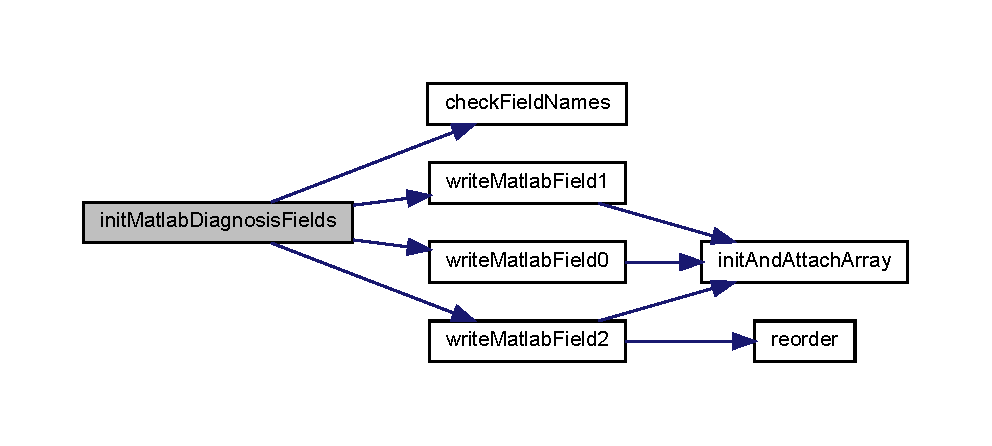
\includegraphics[width=350pt]{namespaceamici_aa12d4917fed647a1edeaaa26a261c770_cgraph}
\end{center}
\end{figure}
\mbox{\Hypertarget{namespaceamici_ad2949f3931c6fac6fd12fd7ede47ac30}\label{namespaceamici_ad2949f3931c6fac6fd12fd7ede47ac30}} 
\index{amici@{amici}!write\+Matlab\+Field0@{write\+Matlab\+Field0}}
\index{write\+Matlab\+Field0@{write\+Matlab\+Field0}!amici@{amici}}
\paragraph{\texorpdfstring{write\+Matlab\+Field0()}{writeMatlabField0()}}
{\footnotesize\ttfamily void write\+Matlab\+Field0 (\begin{DoxyParamCaption}\item[{mx\+Array $\ast$}]{matlab\+Struct,  }\item[{const char $\ast$}]{field\+Name,  }\item[{T}]{field\+Data }\end{DoxyParamCaption})}

initialise vector and attach to the field 
\begin{DoxyParams}{Parameters}
{\em matlab\+Struct} & pointer of the field to which the vector will be attached \\
\hline
{\em field\+Name} & Name of the field to which the vector will be attached \\
\hline
{\em field\+Data} & Data wich will be stored in the field\\
\hline
\end{DoxyParams}
initialise vector and attach to the field 
\begin{DoxyParams}{Parameters}
{\em matlab\+Struct} & pointer of the field to which the vector will be attached \\
\hline
{\em field\+Name} & Name of the field to which the vector will be attached \\
\hline
{\em field\+Data} & Data wich will be stored in the field\\
\hline
\end{DoxyParams}


Definition at line 181 of file returndata\+\_\+matlab.\+cpp.

Here is the call graph for this function\+:
\nopagebreak
\begin{figure}[H]
\begin{center}
\leavevmode
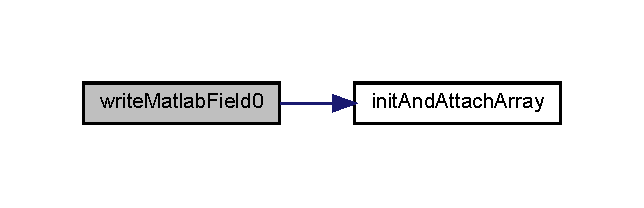
\includegraphics[width=309pt]{namespaceamici_ad2949f3931c6fac6fd12fd7ede47ac30_cgraph}
\end{center}
\end{figure}
Here is the caller graph for this function\+:
\nopagebreak
\begin{figure}[H]
\begin{center}
\leavevmode
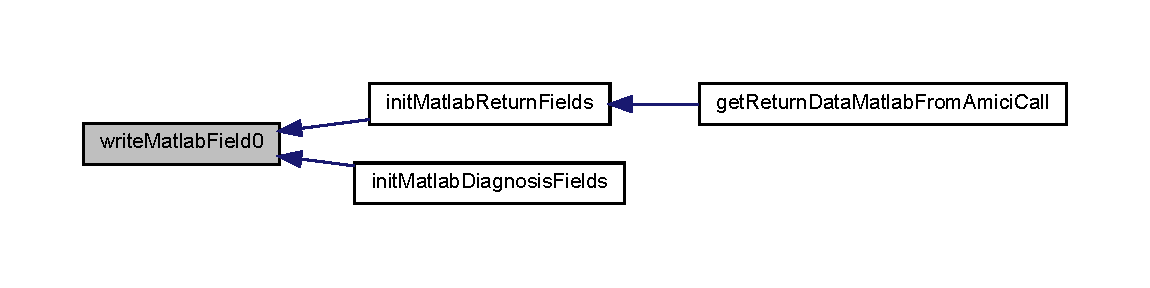
\includegraphics[width=350pt]{namespaceamici_ad2949f3931c6fac6fd12fd7ede47ac30_icgraph}
\end{center}
\end{figure}
\mbox{\Hypertarget{namespaceamici_af4c7cca154fe6e21e8854e1308f1bef7}\label{namespaceamici_af4c7cca154fe6e21e8854e1308f1bef7}} 
\index{amici@{amici}!write\+Matlab\+Field1@{write\+Matlab\+Field1}}
\index{write\+Matlab\+Field1@{write\+Matlab\+Field1}!amici@{amici}}
\paragraph{\texorpdfstring{write\+Matlab\+Field1()}{writeMatlabField1()}}
{\footnotesize\ttfamily void write\+Matlab\+Field1 (\begin{DoxyParamCaption}\item[{mx\+Array $\ast$}]{matlab\+Struct,  }\item[{const char $\ast$}]{field\+Name,  }\item[{std\+::vector$<$ T $>$}]{field\+Data,  }\item[{const int}]{dim0 }\end{DoxyParamCaption})}

initialise vector and attach to the field 
\begin{DoxyParams}{Parameters}
{\em matlab\+Struct} & pointer of the field to which the vector will be attached \\
\hline
{\em field\+Name} & Name of the field to which the vector will be attached \\
\hline
{\em field\+Data} & Data wich will be stored in the field \\
\hline
{\em dim0} & Number of elements in the vector\\
\hline
\end{DoxyParams}
initialise vector and attach to the field 
\begin{DoxyParams}{Parameters}
{\em matlab\+Struct} & pointer of the field to which the vector will be attached \\
\hline
{\em field\+Name} & Name of the field to which the vector will be attached \\
\hline
{\em field\+Data} & Data wich will be stored in the field \\
\hline
{\em dim0} & Number of elements in the vector\\
\hline
\end{DoxyParams}


Definition at line 199 of file returndata\+\_\+matlab.\+cpp.

Here is the call graph for this function\+:
\nopagebreak
\begin{figure}[H]
\begin{center}
\leavevmode
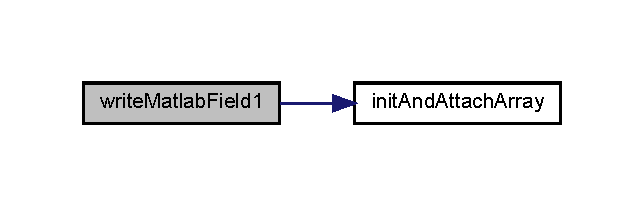
\includegraphics[width=309pt]{namespaceamici_af4c7cca154fe6e21e8854e1308f1bef7_cgraph}
\end{center}
\end{figure}
Here is the caller graph for this function\+:
\nopagebreak
\begin{figure}[H]
\begin{center}
\leavevmode
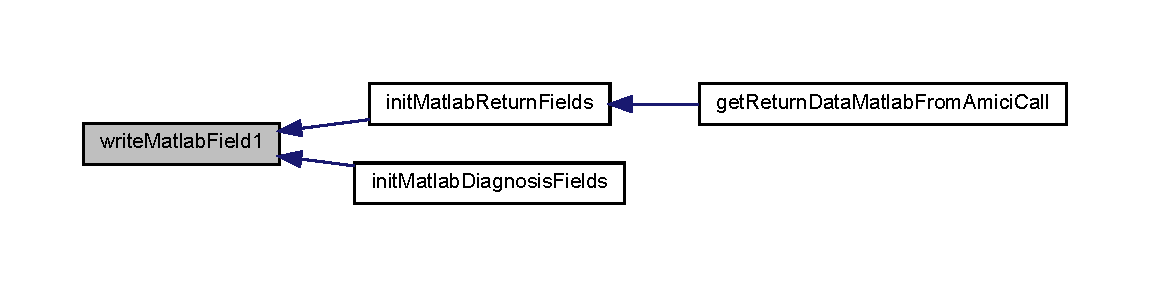
\includegraphics[width=350pt]{namespaceamici_af4c7cca154fe6e21e8854e1308f1bef7_icgraph}
\end{center}
\end{figure}
\mbox{\Hypertarget{namespaceamici_a0a2748c0e1bf95de52a2e2cf3450584e}\label{namespaceamici_a0a2748c0e1bf95de52a2e2cf3450584e}} 
\index{amici@{amici}!write\+Matlab\+Field2@{write\+Matlab\+Field2}}
\index{write\+Matlab\+Field2@{write\+Matlab\+Field2}!amici@{amici}}
\paragraph{\texorpdfstring{write\+Matlab\+Field2()}{writeMatlabField2()}}
{\footnotesize\ttfamily void write\+Matlab\+Field2 (\begin{DoxyParamCaption}\item[{mx\+Array $\ast$}]{matlab\+Struct,  }\item[{const char $\ast$}]{field\+Name,  }\item[{std\+::vector$<$ T $>$}]{field\+Data,  }\item[{int}]{dim0,  }\item[{int}]{dim1,  }\item[{std\+::vector$<$ int $>$}]{perm }\end{DoxyParamCaption})}

initialise matrix, attach to the field and write data 
\begin{DoxyParams}{Parameters}
{\em matlab\+Struct} & Pointer to the matlab structure \\
\hline
{\em field\+Name} & Name of the field to which the tensor will be attached \\
\hline
{\em field\+Data} & Data wich will be stored in the field \\
\hline
{\em dim0} & Number of rows in the tensor \\
\hline
{\em dim1} & Number of columns in the tensor \\
\hline
{\em perm} & reordering of dimensions (i.\+e., transposition)\\
\hline
\end{DoxyParams}
initialise matrix, attach to the field and write data 
\begin{DoxyParams}{Parameters}
{\em matlab\+Struct} & Pointer to the matlab structure \\
\hline
{\em field\+Name} & Name of the field to which the tensor will be attached \\
\hline
{\em field\+Data} & Data wich will be stored in the field \\
\hline
{\em dim0} & Number of rows in the tensor \\
\hline
{\em dim1} & Number of columns in the tensor \\
\hline
{\em perm} & reordering of dimensions (i.\+e., transposition)\\
\hline
\end{DoxyParams}


Definition at line 221 of file returndata\+\_\+matlab.\+cpp.

Here is the call graph for this function\+:
\nopagebreak
\begin{figure}[H]
\begin{center}
\leavevmode
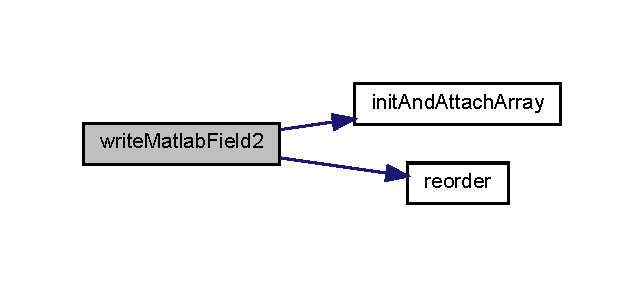
\includegraphics[width=309pt]{namespaceamici_a0a2748c0e1bf95de52a2e2cf3450584e_cgraph}
\end{center}
\end{figure}
Here is the caller graph for this function\+:
\nopagebreak
\begin{figure}[H]
\begin{center}
\leavevmode
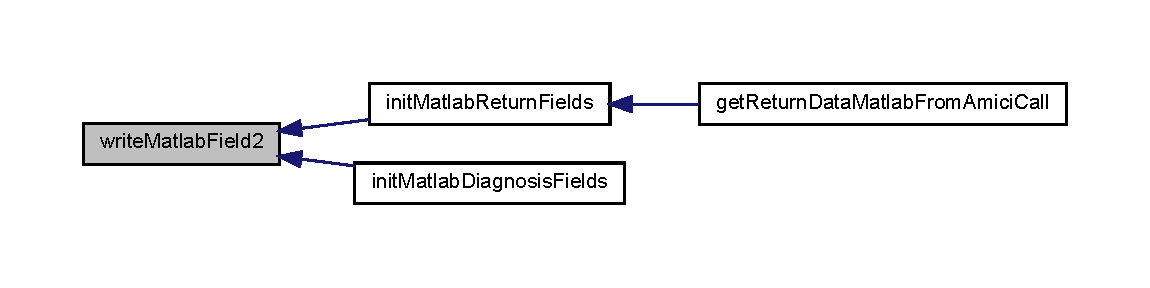
\includegraphics[width=350pt]{namespaceamici_a0a2748c0e1bf95de52a2e2cf3450584e_icgraph}
\end{center}
\end{figure}
\mbox{\Hypertarget{namespaceamici_ae2abb9d1f5b8350ced2799fc10f83ec7}\label{namespaceamici_ae2abb9d1f5b8350ced2799fc10f83ec7}} 
\index{amici@{amici}!write\+Matlab\+Field3@{write\+Matlab\+Field3}}
\index{write\+Matlab\+Field3@{write\+Matlab\+Field3}!amici@{amici}}
\paragraph{\texorpdfstring{write\+Matlab\+Field3()}{writeMatlabField3()}}
{\footnotesize\ttfamily void write\+Matlab\+Field3 (\begin{DoxyParamCaption}\item[{mx\+Array $\ast$}]{matlab\+Struct,  }\item[{const char $\ast$}]{field\+Name,  }\item[{std\+::vector$<$ T $>$}]{field\+Data,  }\item[{int}]{dim0,  }\item[{int}]{dim1,  }\item[{int}]{dim2,  }\item[{std\+::vector$<$ int $>$}]{perm }\end{DoxyParamCaption})}

initialise 3D tensor, attach to the field and write data 
\begin{DoxyParams}{Parameters}
{\em matlab\+Struct} & Pointer to the matlab structure \\
\hline
{\em field\+Name} & Name of the field to which the tensor will be attached \\
\hline
{\em field\+Data} & Data wich will be stored in the field \\
\hline
{\em dim0} & number of rows in the tensor \\
\hline
{\em dim1} & number of columns in the tensor \\
\hline
{\em dim2} & number of elements in the third dimension of the tensor \\
\hline
{\em perm} & reordering of dimensions\\
\hline
\end{DoxyParams}
initialise 3D tensor, attach to the field and write data 
\begin{DoxyParams}{Parameters}
{\em matlab\+Struct} & Pointer to the matlab structure \\
\hline
{\em field\+Name} & Name of the field to which the tensor will be attached \\
\hline
{\em field\+Data} & Data wich will be stored in the field \\
\hline
{\em dim0} & number of rows in the tensor \\
\hline
{\em dim1} & number of columns in the tensor \\
\hline
{\em dim2} & number of elements in the third dimension of the tensor \\
\hline
{\em perm} & reordering of dimensions\\
\hline
\end{DoxyParams}


Definition at line 254 of file returndata\+\_\+matlab.\+cpp.

Here is the call graph for this function\+:
\nopagebreak
\begin{figure}[H]
\begin{center}
\leavevmode
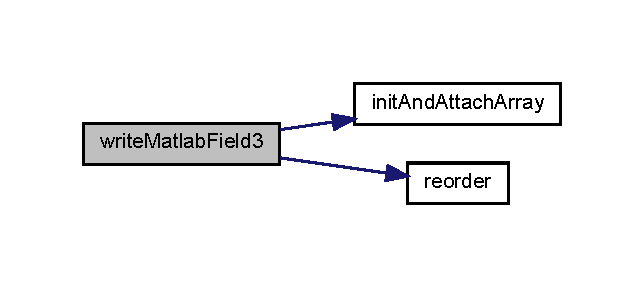
\includegraphics[width=309pt]{namespaceamici_ae2abb9d1f5b8350ced2799fc10f83ec7_cgraph}
\end{center}
\end{figure}
\mbox{\Hypertarget{namespaceamici_a234b1006ff3799742ade304a46ed4965}\label{namespaceamici_a234b1006ff3799742ade304a46ed4965}} 
\index{amici@{amici}!write\+Matlab\+Field4@{write\+Matlab\+Field4}}
\index{write\+Matlab\+Field4@{write\+Matlab\+Field4}!amici@{amici}}
\paragraph{\texorpdfstring{write\+Matlab\+Field4()}{writeMatlabField4()}}
{\footnotesize\ttfamily void write\+Matlab\+Field4 (\begin{DoxyParamCaption}\item[{mx\+Array $\ast$}]{matlab\+Struct,  }\item[{const char $\ast$}]{field\+Name,  }\item[{std\+::vector$<$ T $>$}]{field\+Data,  }\item[{int}]{dim0,  }\item[{int}]{dim1,  }\item[{int}]{dim2,  }\item[{int}]{dim3,  }\item[{std\+::vector$<$ int $>$}]{perm }\end{DoxyParamCaption})}

initialise 4D tensor, attach to the field and write data 
\begin{DoxyParams}{Parameters}
{\em matlab\+Struct} & Pointer to the matlab structure \\
\hline
{\em field\+Name} & Name of the field to which the tensor will be attached \\
\hline
{\em field\+Data} & Data wich will be stored in the field \\
\hline
{\em dim0} & number of rows in the tensor \\
\hline
{\em dim1} & number of columns in the tensor \\
\hline
{\em dim2} & number of elements in the third dimension of the tensor \\
\hline
{\em dim3} & number of elements in the fourth dimension of the tensor \\
\hline
{\em perm} & reordering of dimensions\\
\hline
\end{DoxyParams}
initialise 4D tensor, attach to the field and write data 
\begin{DoxyParams}{Parameters}
{\em matlab\+Struct} & Pointer to the matlab structure \\
\hline
{\em field\+Name} & Name of the field to which the tensor will be attached \\
\hline
{\em field\+Data} & Data wich will be stored in the field \\
\hline
{\em dim0} & number of rows in the tensor \\
\hline
{\em dim1} & number of columns in the tensor \\
\hline
{\em dim2} & number of elements in the third dimension of the tensor \\
\hline
{\em dim3} & number of elements in the fourth dimension of the tensor \\
\hline
{\em perm} & reordering of dimensions\\
\hline
\end{DoxyParams}


Definition at line 290 of file returndata\+\_\+matlab.\+cpp.

Here is the call graph for this function\+:
\nopagebreak
\begin{figure}[H]
\begin{center}
\leavevmode
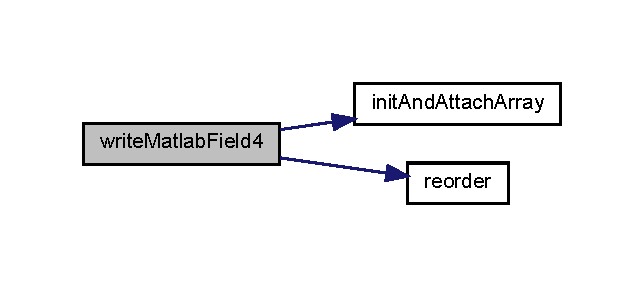
\includegraphics[width=309pt]{namespaceamici_a234b1006ff3799742ade304a46ed4965_cgraph}
\end{center}
\end{figure}
\mbox{\Hypertarget{namespaceamici_a10c4b68cefb537f43f52c1f2f23db5f9}\label{namespaceamici_a10c4b68cefb537f43f52c1f2f23db5f9}} 
\index{amici@{amici}!init\+And\+Attach\+Array@{init\+And\+Attach\+Array}}
\index{init\+And\+Attach\+Array@{init\+And\+Attach\+Array}!amici@{amici}}
\paragraph{\texorpdfstring{init\+And\+Attach\+Array()}{initAndAttachArray()}}
{\footnotesize\ttfamily double $\ast$ init\+And\+Attach\+Array (\begin{DoxyParamCaption}\item[{mx\+Array $\ast$}]{matlab\+Struct,  }\item[{const char $\ast$}]{field\+Name,  }\item[{std\+::vector$<$ mw\+Size $>$}]{dim }\end{DoxyParamCaption})}

initialises the field field\+Name in matlab\+Struct with dimension dim 
\begin{DoxyParams}{Parameters}
{\em matlab\+Struct} & Pointer to the matlab structure \\
\hline
{\em field\+Name} & Name of the field to which the tensor will be attached \\
\hline
{\em dim} & vector of field dimensions\\
\hline
\end{DoxyParams}
\begin{DoxyReturn}{Returns}
Pointer to field data
\end{DoxyReturn}
initialises the field field\+Name in matlab\+Struct with dimension dim 
\begin{DoxyParams}{Parameters}
{\em matlab\+Struct} & Pointer to the matlab structure \\
\hline
{\em field\+Name} & Name of the field to which the tensor will be attached \\
\hline
{\em dim} & vector of field dimensions\\
\hline
\end{DoxyParams}
\begin{DoxyReturn}{Returns}
Pointer to field data
\end{DoxyReturn}


Definition at line 328 of file returndata\+\_\+matlab.\+cpp.

Here is the caller graph for this function\+:
\nopagebreak
\begin{figure}[H]
\begin{center}
\leavevmode
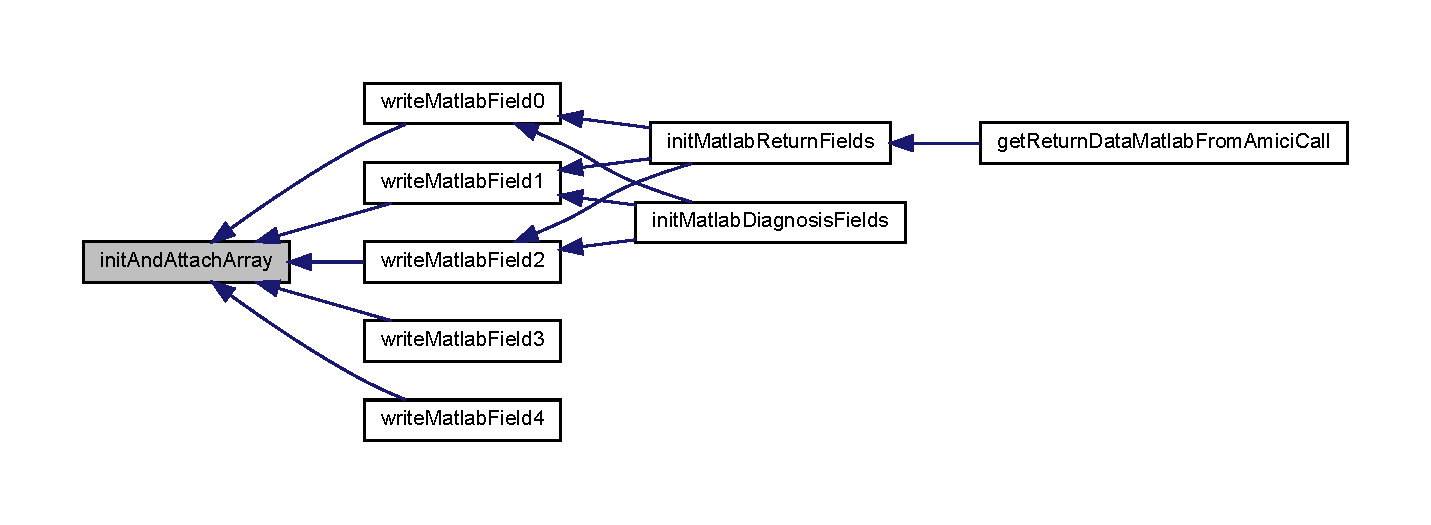
\includegraphics[width=350pt]{namespaceamici_a10c4b68cefb537f43f52c1f2f23db5f9_icgraph}
\end{center}
\end{figure}
\mbox{\Hypertarget{namespaceamici_ad34a0a8f0a3d44e86371a2ecb5841c09}\label{namespaceamici_ad34a0a8f0a3d44e86371a2ecb5841c09}} 
\index{amici@{amici}!check\+Field\+Names@{check\+Field\+Names}}
\index{check\+Field\+Names@{check\+Field\+Names}!amici@{amici}}
\paragraph{\texorpdfstring{check\+Field\+Names()}{checkFieldNames()}}
{\footnotesize\ttfamily void check\+Field\+Names (\begin{DoxyParamCaption}\item[{const char $\ast$$\ast$}]{field\+Names,  }\item[{const int}]{field\+Count }\end{DoxyParamCaption})}

checks whether field\+Names was properly allocated 
\begin{DoxyParams}{Parameters}
{\em field\+Names} & array of field names \\
\hline
{\em field\+Count} & expected number of fields in field\+Names\\
\hline
\end{DoxyParams}
checks whether field\+Names was properly allocated 
\begin{DoxyParams}{Parameters}
{\em field\+Names} & array of field names \\
\hline
{\em field\+Count} & expected number of fields in field\+Names\\
\hline
\end{DoxyParams}


Definition at line 349 of file returndata\+\_\+matlab.\+cpp.

Here is the caller graph for this function\+:
\nopagebreak
\begin{figure}[H]
\begin{center}
\leavevmode
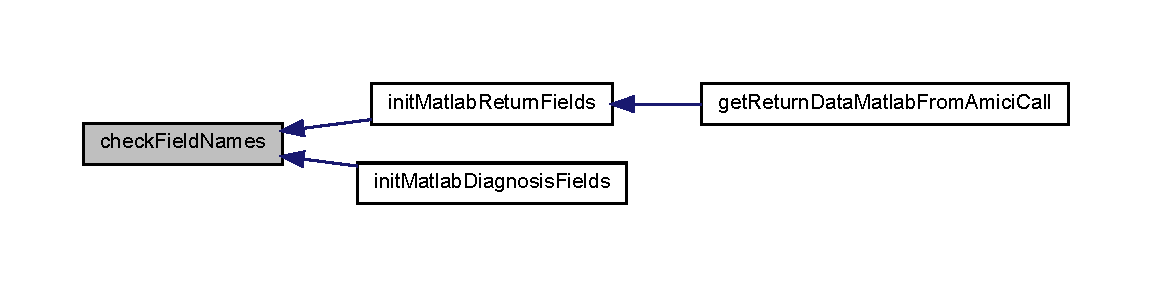
\includegraphics[width=350pt]{namespaceamici_ad34a0a8f0a3d44e86371a2ecb5841c09_icgraph}
\end{center}
\end{figure}
\mbox{\Hypertarget{namespaceamici_ac6d55e052cd87c2cbd7a5a26e8d11628}\label{namespaceamici_ac6d55e052cd87c2cbd7a5a26e8d11628}} 
\index{amici@{amici}!reorder@{reorder}}
\index{reorder@{reorder}!amici@{amici}}
\paragraph{\texorpdfstring{reorder()}{reorder()}}
{\footnotesize\ttfamily std\+::vector$<$ T $>$ reorder (\begin{DoxyParamCaption}\item[{const std\+::vector$<$ T $>$}]{input,  }\item[{const std\+::vector$<$ int $>$}]{order }\end{DoxyParamCaption})}

template function that reorders elements in a std\+::vector


\begin{DoxyParams}{Parameters}
{\em input} & unordered vector \\
\hline
{\em order} & dimension permutation\\
\hline
\end{DoxyParams}
\begin{DoxyReturn}{Returns}
Reordered vector
\end{DoxyReturn}
template function that reorders elements in a std\+::vector


\begin{DoxyParams}{Parameters}
{\em input} & unordered vector \\
\hline
{\em order} & dimension permutation\\
\hline
\end{DoxyParams}
\begin{DoxyReturn}{Returns}
Reordered vector
\end{DoxyReturn}


Definition at line 362 of file returndata\+\_\+matlab.\+cpp.

Here is the caller graph for this function\+:
\nopagebreak
\begin{figure}[H]
\begin{center}
\leavevmode
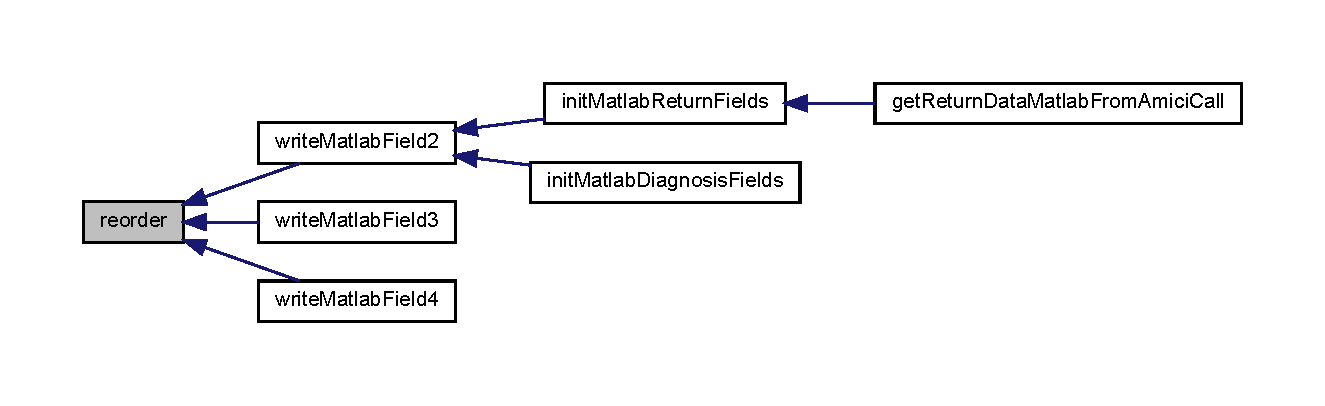
\includegraphics[width=350pt]{namespaceamici_ac6d55e052cd87c2cbd7a5a26e8d11628_icgraph}
\end{center}
\end{figure}
\mbox{\Hypertarget{namespaceamici_a042a9a4166aeef6cd263d9975a4192ed}\label{namespaceamici_a042a9a4166aeef6cd263d9975a4192ed}} 
\index{amici@{amici}!serialize\+To\+Char@{serialize\+To\+Char}}
\index{serialize\+To\+Char@{serialize\+To\+Char}!amici@{amici}}
\paragraph{\texorpdfstring{serialize\+To\+Char()}{serializeToChar()}}
{\footnotesize\ttfamily char$\ast$ amici\+::serialize\+To\+Char (\begin{DoxyParamCaption}\item[{T const \&}]{data,  }\item[{int $\ast$}]{size }\end{DoxyParamCaption})}

Serialize object to char array


\begin{DoxyParams}{Parameters}
{\em data} & input object \\
\hline
{\em size} & maximum char length\\
\hline
\end{DoxyParams}
\begin{DoxyReturn}{Returns}
The object serialized as char
\end{DoxyReturn}


Definition at line 172 of file serialization.\+h.

\mbox{\Hypertarget{namespaceamici_ad633859edca1bf95ecdbdb5500d3c28c}\label{namespaceamici_ad633859edca1bf95ecdbdb5500d3c28c}} 
\index{amici@{amici}!deserialize\+From\+Char@{deserialize\+From\+Char}}
\index{deserialize\+From\+Char@{deserialize\+From\+Char}!amici@{amici}}
\paragraph{\texorpdfstring{deserialize\+From\+Char()}{deserializeFromChar()}}
{\footnotesize\ttfamily T amici\+::deserialize\+From\+Char (\begin{DoxyParamCaption}\item[{const char $\ast$}]{buffer,  }\item[{int}]{size }\end{DoxyParamCaption})}

Deserialize object that has been serialized using serialize\+To\+Char


\begin{DoxyParams}{Parameters}
{\em buffer} & serialized object \\
\hline
{\em size} & length of buffer\\
\hline
\end{DoxyParams}
\begin{DoxyReturn}{Returns}
The deserialized object
\end{DoxyReturn}


Definition at line 205 of file serialization.\+h.

\mbox{\Hypertarget{namespaceamici_aed4ae7f193798ade342a0f70491e849e}\label{namespaceamici_aed4ae7f193798ade342a0f70491e849e}} 
\index{amici@{amici}!serialize\+To\+String@{serialize\+To\+String}}
\index{serialize\+To\+String@{serialize\+To\+String}!amici@{amici}}
\paragraph{\texorpdfstring{serialize\+To\+String()}{serializeToString()}}
{\footnotesize\ttfamily std\+::string amici\+::serialize\+To\+String (\begin{DoxyParamCaption}\item[{T const \&}]{data }\end{DoxyParamCaption})}

Serialize object to string


\begin{DoxyParams}{Parameters}
{\em data} & input object\\
\hline
\end{DoxyParams}
\begin{DoxyReturn}{Returns}
The object serialized as string
\end{DoxyReturn}


Definition at line 230 of file serialization.\+h.

\mbox{\Hypertarget{namespaceamici_ad5b38b6ae6007acbaf43521f2a616937}\label{namespaceamici_ad5b38b6ae6007acbaf43521f2a616937}} 
\index{amici@{amici}!serialize\+To\+Std\+Vec@{serialize\+To\+Std\+Vec}}
\index{serialize\+To\+Std\+Vec@{serialize\+To\+Std\+Vec}!amici@{amici}}
\paragraph{\texorpdfstring{serialize\+To\+Std\+Vec()}{serializeToStdVec()}}
{\footnotesize\ttfamily std\+::vector$<$char$>$ amici\+::serialize\+To\+Std\+Vec (\begin{DoxyParamCaption}\item[{T const \&}]{data }\end{DoxyParamCaption})}

Serialize object to std\+::vector$<$char$>$


\begin{DoxyParams}{Parameters}
{\em data} & input object\\
\hline
\end{DoxyParams}
\begin{DoxyReturn}{Returns}
The object serialized as std\+::vector$<$char$>$
\end{DoxyReturn}


Definition at line 256 of file serialization.\+h.

\mbox{\Hypertarget{namespaceamici_a863d35f9934623bc5f7f409a05fa0d67}\label{namespaceamici_a863d35f9934623bc5f7f409a05fa0d67}} 
\index{amici@{amici}!deserialize\+From\+String@{deserialize\+From\+String}}
\index{deserialize\+From\+String@{deserialize\+From\+String}!amici@{amici}}
\paragraph{\texorpdfstring{deserialize\+From\+String()}{deserializeFromString()}}
{\footnotesize\ttfamily T amici\+::deserialize\+From\+String (\begin{DoxyParamCaption}\item[{std\+::string const \&}]{serialized }\end{DoxyParamCaption})}

Deserialize object that has been serialized using serialize\+To\+String


\begin{DoxyParams}{Parameters}
{\em serialized} & serialized object\\
\hline
\end{DoxyParams}
\begin{DoxyReturn}{Returns}
The deserialized object
\end{DoxyReturn}


Definition at line 283 of file serialization.\+h.

\mbox{\Hypertarget{namespaceamici_a252a116a8f94abccc25b2086deb0734b}\label{namespaceamici_a252a116a8f94abccc25b2086deb0734b}} 
\index{amici@{amici}!operator==@{operator==}}
\index{operator==@{operator==}!amici@{amici}}
\paragraph{\texorpdfstring{operator==()}{operator==()}\hspace{0.1cm}{\footnotesize\ttfamily [2/2]}}
{\footnotesize\ttfamily bool operator== (\begin{DoxyParamCaption}\item[{const \mbox{\hyperlink{classamici_1_1_solver}{Solver}} \&}]{a,  }\item[{const \mbox{\hyperlink{classamici_1_1_solver}{Solver}} \&}]{b }\end{DoxyParamCaption})}


\begin{DoxyParams}{Parameters}
{\em a} & \\
\hline
{\em b} & \\
\hline
\end{DoxyParams}
\begin{DoxyReturn}{Returns}

\end{DoxyReturn}


Definition at line 378 of file solver.\+cpp.

Here is the call graph for this function\+:
\nopagebreak
\begin{figure}[H]
\begin{center}
\leavevmode
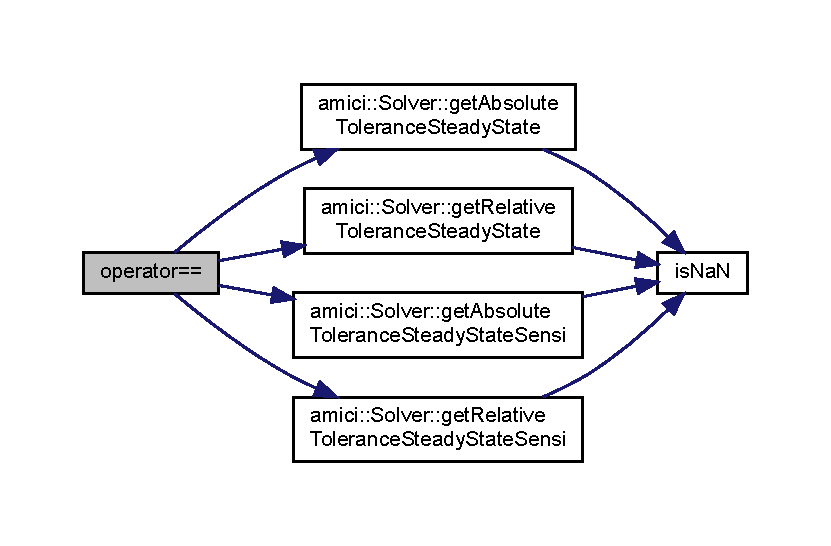
\includegraphics[width=350pt]{namespaceamici_a252a116a8f94abccc25b2086deb0734b_cgraph}
\end{center}
\end{figure}
\mbox{\Hypertarget{namespaceamici_aa6801bbdb0c7625719c019ac287be29e}\label{namespaceamici_aa6801bbdb0c7625719c019ac287be29e}} 
\index{amici@{amici}!spline@{spline}}
\index{spline@{spline}!amici@{amici}}
\paragraph{\texorpdfstring{spline()}{spline()}\hspace{0.1cm}{\footnotesize\ttfamily [1/2]}}
{\footnotesize\ttfamily int spline (\begin{DoxyParamCaption}\item[{int}]{n,  }\item[{int}]{end1,  }\item[{int}]{end2,  }\item[{double}]{slope1,  }\item[{double}]{slope2,  }\item[{double}]{x\mbox{[}$\,$\mbox{]},  }\item[{double}]{y\mbox{[}$\,$\mbox{]},  }\item[{double}]{b\mbox{[}$\,$\mbox{]},  }\item[{double}]{c\mbox{[}$\,$\mbox{]},  }\item[{double}]{d\mbox{[}$\,$\mbox{]} }\end{DoxyParamCaption})}

Evaluate the coefficients b\mbox{[}i\mbox{]}, c\mbox{[}i\mbox{]}, d\mbox{[}i\mbox{]}, i = 0, 1, .. n-\/1 for a cubic interpolating spline

S(xx) = Y\mbox{[}i\mbox{]} + b\mbox{[}i\mbox{]} $\ast$ w + c\mbox{[}i\mbox{]} $\ast$ w$\ast$$\ast$2 + d\mbox{[}i\mbox{]} $\ast$ w$\ast$$\ast$3 where w = xx -\/ x\mbox{[}i\mbox{]} and x\mbox{[}i\mbox{]} $<$= xx $<$= x\mbox{[}i+1\mbox{]}

The n supplied data points are x\mbox{[}i\mbox{]}, y\mbox{[}i\mbox{]}, i = 0 ... n-\/1.


\begin{DoxyParams}[1]{Parameters}
\mbox{\tt in}  & {\em n} & The number of data points or knots (n $>$= 2) \\
\hline
\mbox{\tt in}  & {\em end1} & 0\+: default condition 1\+: specify the slopes at x\mbox{[}0\mbox{]} \\
\hline
\mbox{\tt in}  & {\em end2} & 0\+: default condition 1\+: specify the slopes at x\mbox{[}n-\/1\mbox{]} \\
\hline
\mbox{\tt in}  & {\em slope1} & slope at x\mbox{[}0\mbox{]} \\
\hline
\mbox{\tt in}  & {\em slope2} & slope at x\mbox{[}n-\/1\mbox{]} \\
\hline
\mbox{\tt in}  & {\em x\mbox{[}$\,$\mbox{]}} & the abscissas of the knots in strictly increasing order \\
\hline
\mbox{\tt in}  & {\em y\mbox{[}$\,$\mbox{]}} & the ordinates of the knots \\
\hline
\mbox{\tt out}  & {\em b\mbox{[}$\,$\mbox{]}} & array of spline coefficients \\
\hline
\mbox{\tt out}  & {\em c\mbox{[}$\,$\mbox{]}} & array of spline coefficients \\
\hline
\mbox{\tt out}  & {\em d\mbox{[}$\,$\mbox{]}} & array of spline coefficients\\
\hline
\end{DoxyParams}

\begin{DoxyRetVals}{Return values}
{\em 0} & normal return \\
\hline
{\em 1} & less than two data points; cannot interpolate \\
\hline
{\em 2} & x\mbox{[}\mbox{]} are not in ascending order\\
\hline
\end{DoxyRetVals}
\paragraph*{Notes }


\begin{DoxyItemize}
\item The accompanying function \mbox{\hyperlink{namespaceamici_a20c8c27889853621fba3e0eacd333723}{seval()}} may be used to evaluate the spline while deriv will provide the first derivative.
\item Using p to denote differentiation y\mbox{[}i\mbox{]} = S(\+X\mbox{[}i\mbox{]}) b\mbox{[}i\mbox{]} = Sp(\+X\mbox{[}i\mbox{]}) c\mbox{[}i\mbox{]} = Spp(\+X\mbox{[}i\mbox{]})/2 d\mbox{[}i\mbox{]} = Sppp(\+X\mbox{[}i\mbox{]})/6 ( Derivative from the right )
\item Since the zero elements of the arrays A\+RE N\+OW used here, all arrays to be passed from the main program should be dimensioned at least \mbox{[}n\mbox{]}. These routines will use elements \mbox{[}0 .. n-\/1\mbox{]}.
\item Adapted from the text Forsythe, G.\+E., Malcolm, M.\+A. and Moler, C.\+B. (1977) \char`\"{}\+Computer Methods for Mathematical Computations\char`\"{} Prentice Hall
\item Note that although there are only n-\/1 polynomial segments, n elements are requird in b, c, d. The elements b\mbox{[}n-\/1\mbox{]}, c\mbox{[}n-\/1\mbox{]} and d\mbox{[}n-\/1\mbox{]} are set to continue the last segment past x\mbox{[}n-\/1\mbox{]}. 
\end{DoxyItemize}

Definition at line 16 of file spline.\+cpp.

Here is the caller graph for this function\+:
\nopagebreak
\begin{figure}[H]
\begin{center}
\leavevmode
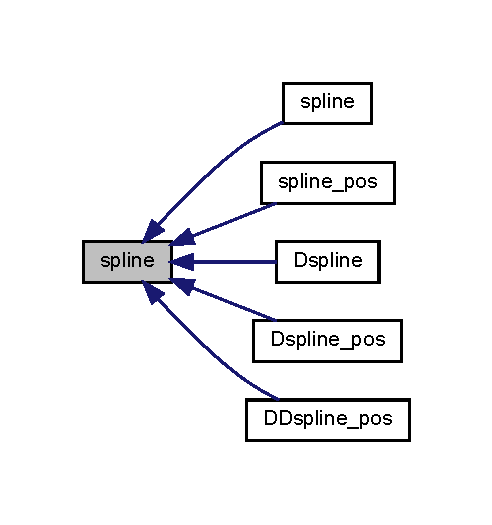
\includegraphics[width=236pt]{namespaceamici_aa6801bbdb0c7625719c019ac287be29e_icgraph}
\end{center}
\end{figure}
\mbox{\Hypertarget{namespaceamici_a20c8c27889853621fba3e0eacd333723}\label{namespaceamici_a20c8c27889853621fba3e0eacd333723}} 
\index{amici@{amici}!seval@{seval}}
\index{seval@{seval}!amici@{amici}}
\paragraph{\texorpdfstring{seval()}{seval()}}
{\footnotesize\ttfamily double seval (\begin{DoxyParamCaption}\item[{int}]{n,  }\item[{double}]{u,  }\item[{double}]{x\mbox{[}$\,$\mbox{]},  }\item[{double}]{y\mbox{[}$\,$\mbox{]},  }\item[{double}]{b\mbox{[}$\,$\mbox{]},  }\item[{double}]{c\mbox{[}$\,$\mbox{]},  }\item[{double}]{d\mbox{[}$\,$\mbox{]} }\end{DoxyParamCaption})}

S(xx) = y\mbox{[}i\mbox{]} + b\mbox{[}i\mbox{]} $\ast$ w + c\mbox{[}i\mbox{]} $\ast$ w$\ast$$\ast$2 + d\mbox{[}i\mbox{]} $\ast$ w$\ast$$\ast$3 where w = u -\/ x\mbox{[}i\mbox{]} and x\mbox{[}i\mbox{]} $<$= u $<$= x\mbox{[}i+1\mbox{]} Note that Horner\textquotesingle{}s rule is used. If u $<$ x\mbox{[}0\mbox{]} then i = 0 is used. If u $>$ x\mbox{[}n-\/1\mbox{]} then i = n-\/1 is used.


\begin{DoxyParams}[1]{Parameters}
\mbox{\tt in}  & {\em n} & The number of data points or knots (n $>$= 2) \\
\hline
\mbox{\tt in}  & {\em u} & the abscissa at which the spline is to be evaluated \\
\hline
\mbox{\tt in}  & {\em x\mbox{[}$\,$\mbox{]}} & the abscissas of the knots in strictly increasing order \\
\hline
\mbox{\tt in}  & {\em y\mbox{[}$\,$\mbox{]}} & the ordinates of the knots \\
\hline
\mbox{\tt in}  & {\em b} & array of spline coefficients computed by \mbox{\hyperlink{namespaceamici_aa6801bbdb0c7625719c019ac287be29e}{spline()}}. \\
\hline
\mbox{\tt in}  & {\em c} & array of spline coefficients computed by \mbox{\hyperlink{namespaceamici_aa6801bbdb0c7625719c019ac287be29e}{spline()}}. \\
\hline
\mbox{\tt in}  & {\em d} & array of spline coefficients computed by \mbox{\hyperlink{namespaceamici_aa6801bbdb0c7625719c019ac287be29e}{spline()}}.\\
\hline
\end{DoxyParams}
\begin{DoxyReturn}{Returns}
the value of the spline function at u
\end{DoxyReturn}
Notes
\begin{DoxyItemize}
\item If u is not in the same interval as the previous call then a binary search is performed to determine the proper interval. 
\end{DoxyItemize}

Definition at line 195 of file spline.\+cpp.

Here is the caller graph for this function\+:
\nopagebreak
\begin{figure}[H]
\begin{center}
\leavevmode
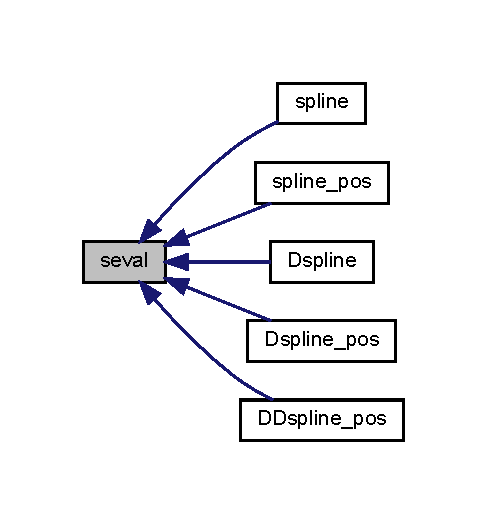
\includegraphics[width=234pt]{namespaceamici_a20c8c27889853621fba3e0eacd333723_icgraph}
\end{center}
\end{figure}
\mbox{\Hypertarget{namespaceamici_a158da90aec69a4796fb6f350ac6b71ab}\label{namespaceamici_a158da90aec69a4796fb6f350ac6b71ab}} 
\index{amici@{amici}!sinteg@{sinteg}}
\index{sinteg@{sinteg}!amici@{amici}}
\paragraph{\texorpdfstring{sinteg()}{sinteg()}}
{\footnotesize\ttfamily double sinteg (\begin{DoxyParamCaption}\item[{int}]{n,  }\item[{double}]{u,  }\item[{double}]{x\mbox{[}$\,$\mbox{]},  }\item[{double}]{y\mbox{[}$\,$\mbox{]},  }\item[{double}]{b\mbox{[}$\,$\mbox{]},  }\item[{double}]{c\mbox{[}$\,$\mbox{]},  }\item[{double}]{d\mbox{[}$\,$\mbox{]} }\end{DoxyParamCaption})}

Integrate the cubic spline function

S(xx) = y\mbox{[}i\mbox{]} + b\mbox{[}i\mbox{]} $\ast$ w + c\mbox{[}i\mbox{]} $\ast$ w$\ast$$\ast$2 + d\mbox{[}i\mbox{]} $\ast$ w$\ast$$\ast$3 where w = u -\/ x\mbox{[}i\mbox{]} and x\mbox{[}i\mbox{]} $<$= u $<$= x\mbox{[}i+1\mbox{]}

The integral is zero at u = x\mbox{[}0\mbox{]}.

If u $<$ x\mbox{[}0\mbox{]} then i = 0 segment is extrapolated. If u $>$ x\mbox{[}n-\/1\mbox{]} then i = n-\/1 segment is extrapolated.


\begin{DoxyParams}[1]{Parameters}
\mbox{\tt in}  & {\em n} & the number of data points or knots (n $>$= 2) \\
\hline
\mbox{\tt in}  & {\em u} & the abscissa at which the spline is to be evaluated \\
\hline
\mbox{\tt in}  & {\em x\mbox{[}$\,$\mbox{]}} & the abscissas of the knots in strictly increasing order \\
\hline
\mbox{\tt in}  & {\em y\mbox{[}$\,$\mbox{]}} & the ordinates of the knots \\
\hline
\mbox{\tt in}  & {\em b} & array of spline coefficients computed by \mbox{\hyperlink{namespaceamici_aa6801bbdb0c7625719c019ac287be29e}{spline()}}. \\
\hline
\mbox{\tt in}  & {\em c} & array of spline coefficients computed by \mbox{\hyperlink{namespaceamici_aa6801bbdb0c7625719c019ac287be29e}{spline()}}. \\
\hline
\mbox{\tt in}  & {\em d} & array of spline coefficients computed by \mbox{\hyperlink{namespaceamici_aa6801bbdb0c7625719c019ac287be29e}{spline()}}.\\
\hline
\end{DoxyParams}
\begin{DoxyReturn}{Returns}
the value of the spline function at u
\end{DoxyReturn}
Notes
\begin{DoxyItemize}
\item If u is not in the same interval as the previous call then a binary search is performed to determine the proper interval. 
\end{DoxyItemize}

Definition at line 256 of file spline.\+cpp.

\mbox{\Hypertarget{namespaceamici_adb302c9aafbaa5e180d9f60ee954bb82}\label{namespaceamici_adb302c9aafbaa5e180d9f60ee954bb82}} 
\index{amici@{amici}!log@{log}}
\index{log@{log}!amici@{amici}}
\paragraph{\texorpdfstring{log()}{log()}}
{\footnotesize\ttfamily double log (\begin{DoxyParamCaption}\item[{double}]{x }\end{DoxyParamCaption})}

c implementation of log function, this prevents returning NaN values for negative values


\begin{DoxyParams}{Parameters}
{\em x} & argument \\
\hline
\end{DoxyParams}
\begin{DoxyReturn}{Returns}
if(x$>$0) then log(x) else -\/\+Inf 
\end{DoxyReturn}


Definition at line 62 of file symbolic\+\_\+functions.\+cpp.

Here is the caller graph for this function\+:
\nopagebreak
\begin{figure}[H]
\begin{center}
\leavevmode
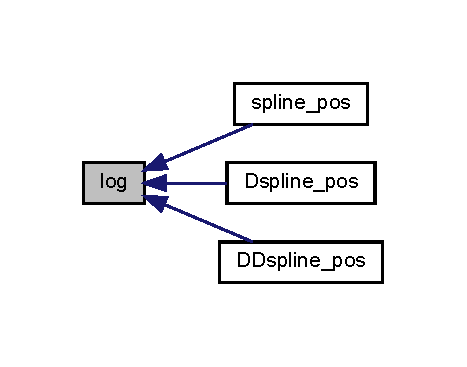
\includegraphics[width=224pt]{namespaceamici_adb302c9aafbaa5e180d9f60ee954bb82_icgraph}
\end{center}
\end{figure}
\mbox{\Hypertarget{namespaceamici_a30a33546875b9dd1a63c29312b316f7e}\label{namespaceamici_a30a33546875b9dd1a63c29312b316f7e}} 
\index{amici@{amici}!dirac@{dirac}}
\index{dirac@{dirac}!amici@{amici}}
\paragraph{\texorpdfstring{dirac()}{dirac()}}
{\footnotesize\ttfamily double dirac (\begin{DoxyParamCaption}\item[{double}]{x }\end{DoxyParamCaption})}

c implementation of matlab function dirac


\begin{DoxyParams}{Parameters}
{\em x} & argument \\
\hline
\end{DoxyParams}
\begin{DoxyReturn}{Returns}
if(x==0) then I\+NF else 0 
\end{DoxyReturn}


Definition at line 77 of file symbolic\+\_\+functions.\+cpp.

\mbox{\Hypertarget{namespaceamici_a609b523b00064e82442c1f1519f40bdb}\label{namespaceamici_a609b523b00064e82442c1f1519f40bdb}} 
\index{amici@{amici}!heaviside@{heaviside}}
\index{heaviside@{heaviside}!amici@{amici}}
\paragraph{\texorpdfstring{heaviside()}{heaviside()}}
{\footnotesize\ttfamily double heaviside (\begin{DoxyParamCaption}\item[{double}]{x }\end{DoxyParamCaption})}

c implementation of matlab function heaviside


\begin{DoxyParams}{Parameters}
{\em x} & argument \\
\hline
\end{DoxyParams}
\begin{DoxyReturn}{Returns}
if(x$>$0) then 1 else 0 
\end{DoxyReturn}


Definition at line 92 of file symbolic\+\_\+functions.\+cpp.

\mbox{\Hypertarget{namespaceamici_a0e1665a05c4dfee1572bea48f7930502}\label{namespaceamici_a0e1665a05c4dfee1572bea48f7930502}} 
\index{amici@{amici}!min@{min}}
\index{min@{min}!amici@{amici}}
\paragraph{\texorpdfstring{min()}{min()}}
{\footnotesize\ttfamily double min (\begin{DoxyParamCaption}\item[{double}]{a,  }\item[{double}]{b,  }\item[{double}]{c }\end{DoxyParamCaption})}

c implementation of matlab function min


\begin{DoxyParams}{Parameters}
{\em a} & value1 \\
\hline
{\em b} & value2 \\
\hline
{\em c} & bogus parameter to ensure correct parsing as a function \\
\hline
\end{DoxyParams}
\begin{DoxyReturn}{Returns}
if(a $<$ b) then a else b 
\end{DoxyReturn}


Definition at line 149 of file symbolic\+\_\+functions.\+cpp.

Here is the call graph for this function\+:
\nopagebreak
\begin{figure}[H]
\begin{center}
\leavevmode
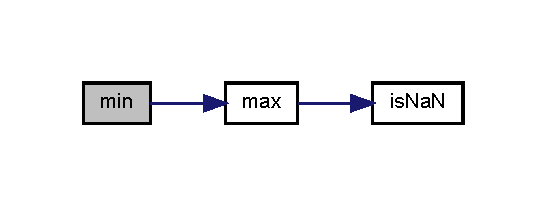
\includegraphics[width=262pt]{namespaceamici_a0e1665a05c4dfee1572bea48f7930502_cgraph}
\end{center}
\end{figure}
Here is the caller graph for this function\+:
\nopagebreak
\begin{figure}[H]
\begin{center}
\leavevmode
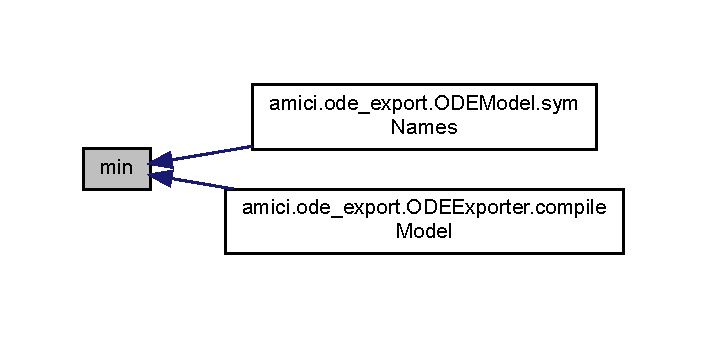
\includegraphics[width=339pt]{namespaceamici_a0e1665a05c4dfee1572bea48f7930502_icgraph}
\end{center}
\end{figure}
\mbox{\Hypertarget{namespaceamici_a6eab5ae993f16386289c3d3e7da90435}\label{namespaceamici_a6eab5ae993f16386289c3d3e7da90435}} 
\index{amici@{amici}!Dmin@{Dmin}}
\index{Dmin@{Dmin}!amici@{amici}}
\paragraph{\texorpdfstring{Dmin()}{Dmin()}}
{\footnotesize\ttfamily double Dmin (\begin{DoxyParamCaption}\item[{int}]{id,  }\item[{double}]{a,  }\item[{double}]{b,  }\item[{double}]{c }\end{DoxyParamCaption})}

parameter derivative of c implementation of matlab function max


\begin{DoxyParams}{Parameters}
{\em id} & argument index for differentiation \\
\hline
{\em a} & value1 \\
\hline
{\em b} & value2 \\
\hline
{\em c} & bogus parameter to ensure correct parsing as a function \\
\hline
\end{DoxyParams}
\begin{DoxyReturn}{Returns}
id == 1\+: if(a $>$ b) then 1 else 0 

id == 2\+: if(a $>$ b) then 0 else 1 
\end{DoxyReturn}


Definition at line 191 of file symbolic\+\_\+functions.\+cpp.

Here is the call graph for this function\+:
\nopagebreak
\begin{figure}[H]
\begin{center}
\leavevmode
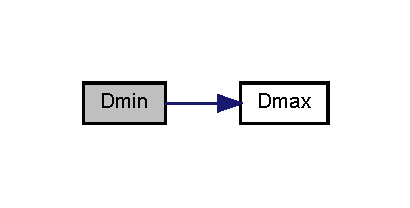
\includegraphics[width=197pt]{namespaceamici_a6eab5ae993f16386289c3d3e7da90435_cgraph}
\end{center}
\end{figure}
\mbox{\Hypertarget{namespaceamici_a98d705fa2f3a5e7566f99fc26d1573de}\label{namespaceamici_a98d705fa2f3a5e7566f99fc26d1573de}} 
\index{amici@{amici}!max@{max}}
\index{max@{max}!amici@{amici}}
\paragraph{\texorpdfstring{max()}{max()}}
{\footnotesize\ttfamily double max (\begin{DoxyParamCaption}\item[{double}]{a,  }\item[{double}]{b,  }\item[{double}]{c }\end{DoxyParamCaption})}

c implementation of matlab function max


\begin{DoxyParams}{Parameters}
{\em a} & value1 \\
\hline
{\em b} & value2 \\
\hline
{\em c} & bogus parameter to ensure correct parsing as a function \\
\hline
\end{DoxyParams}
\begin{DoxyReturn}{Returns}
if(a $>$ b) then a else b 
\end{DoxyReturn}


Definition at line 128 of file symbolic\+\_\+functions.\+cpp.

Here is the call graph for this function\+:
\nopagebreak
\begin{figure}[H]
\begin{center}
\leavevmode
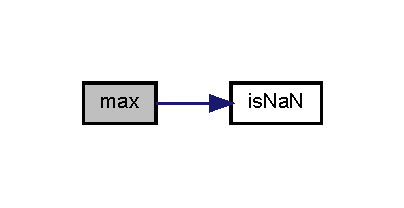
\includegraphics[width=194pt]{namespaceamici_a98d705fa2f3a5e7566f99fc26d1573de_cgraph}
\end{center}
\end{figure}
Here is the caller graph for this function\+:
\nopagebreak
\begin{figure}[H]
\begin{center}
\leavevmode
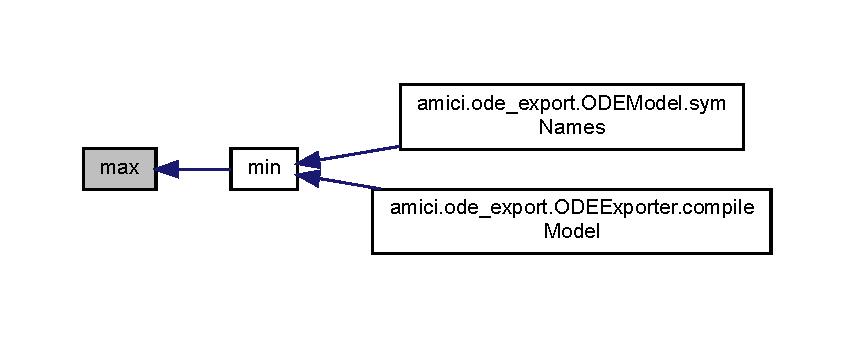
\includegraphics[width=350pt]{namespaceamici_a98d705fa2f3a5e7566f99fc26d1573de_icgraph}
\end{center}
\end{figure}
\mbox{\Hypertarget{namespaceamici_a9afb37cc1fa38a1bfa427f9c27255e5b}\label{namespaceamici_a9afb37cc1fa38a1bfa427f9c27255e5b}} 
\index{amici@{amici}!Dmax@{Dmax}}
\index{Dmax@{Dmax}!amici@{amici}}
\paragraph{\texorpdfstring{Dmax()}{Dmax()}}
{\footnotesize\ttfamily double Dmax (\begin{DoxyParamCaption}\item[{int}]{id,  }\item[{double}]{a,  }\item[{double}]{b,  }\item[{double}]{c }\end{DoxyParamCaption})}

parameter derivative of c implementation of matlab function max


\begin{DoxyParams}{Parameters}
{\em id} & argument index for differentiation \\
\hline
{\em a} & value1 \\
\hline
{\em b} & value2 \\
\hline
{\em c} & bogus parameter to ensure correct parsing as a function \\
\hline
\end{DoxyParams}
\begin{DoxyReturn}{Returns}
id == 1\+: if(a $>$ b) then 1 else 0 

id == 2\+: if(a $>$ b) then 0 else 1 
\end{DoxyReturn}


Definition at line 164 of file symbolic\+\_\+functions.\+cpp.

Here is the caller graph for this function\+:
\nopagebreak
\begin{figure}[H]
\begin{center}
\leavevmode
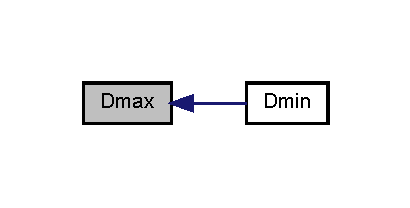
\includegraphics[width=197pt]{namespaceamici_a9afb37cc1fa38a1bfa427f9c27255e5b_icgraph}
\end{center}
\end{figure}
\mbox{\Hypertarget{namespaceamici_af596fe82a4ff6588a527a73d659c4db6}\label{namespaceamici_af596fe82a4ff6588a527a73d659c4db6}} 
\index{amici@{amici}!pos\+\_\+pow@{pos\+\_\+pow}}
\index{pos\+\_\+pow@{pos\+\_\+pow}!amici@{amici}}
\paragraph{\texorpdfstring{pos\+\_\+pow()}{pos\_pow()}}
{\footnotesize\ttfamily double pos\+\_\+pow (\begin{DoxyParamCaption}\item[{double}]{base,  }\item[{double}]{exponent }\end{DoxyParamCaption})}

specialized pow functions that assumes positivity of the first argument


\begin{DoxyParams}{Parameters}
{\em base} & base \\
\hline
{\em exponent} & exponent \\
\hline
\end{DoxyParams}
\begin{DoxyReturn}{Returns}
pow(max(base,0.\+0),exponen) 
\end{DoxyReturn}


Definition at line 203 of file symbolic\+\_\+functions.\+cpp.

\mbox{\Hypertarget{namespaceamici_a7452657cd5f8d541f9e823df5e82c516}\label{namespaceamici_a7452657cd5f8d541f9e823df5e82c516}} 
\index{amici@{amici}!is\+NaN@{is\+NaN}}
\index{is\+NaN@{is\+NaN}!amici@{amici}}
\paragraph{\texorpdfstring{is\+Na\+N()}{isNaN()}}
{\footnotesize\ttfamily int is\+NaN (\begin{DoxyParamCaption}\item[{double}]{what }\end{DoxyParamCaption})}

c++ interface to the is\+NaN function


\begin{DoxyParams}{Parameters}
{\em what} & argument \\
\hline
\end{DoxyParams}
\begin{DoxyReturn}{Returns}
isnan(what) 
\end{DoxyReturn}


Definition at line 35 of file symbolic\+\_\+functions.\+cpp.

Here is the caller graph for this function\+:
\nopagebreak
\begin{figure}[H]
\begin{center}
\leavevmode
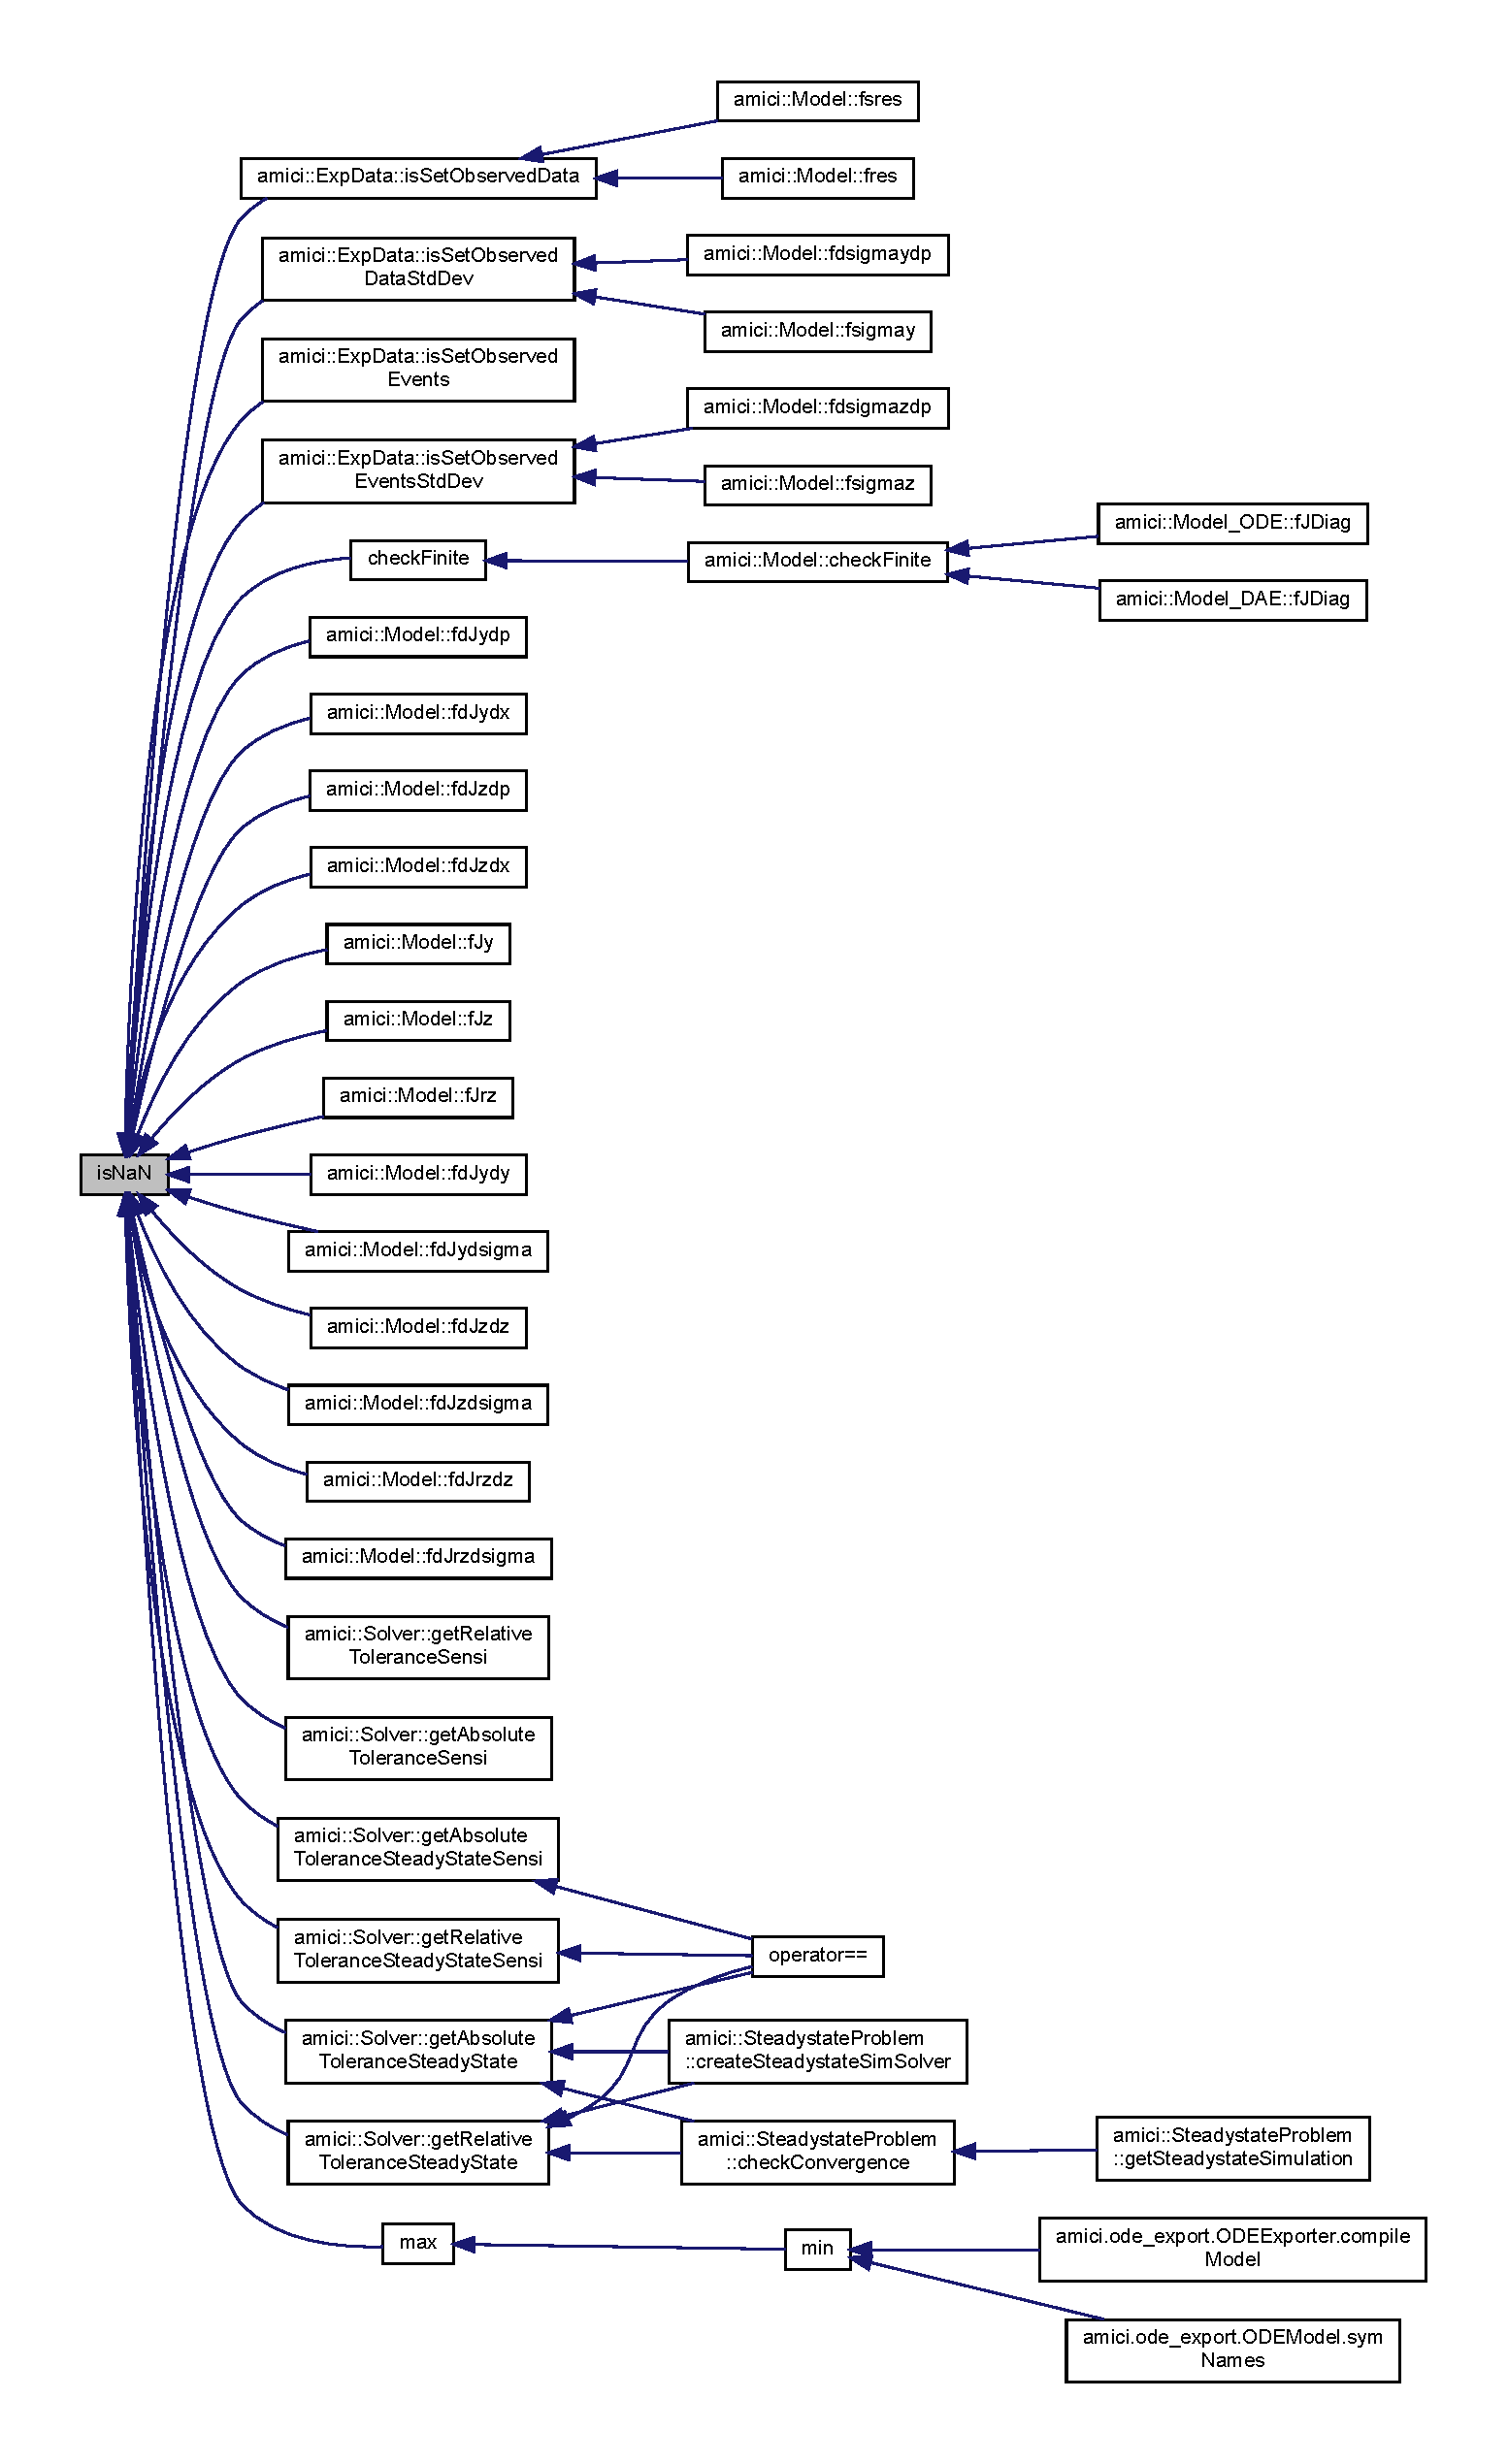
\includegraphics[height=550pt]{namespaceamici_a7452657cd5f8d541f9e823df5e82c516_icgraph}
\end{center}
\end{figure}
\mbox{\Hypertarget{namespaceamici_a10c0a2eb43575a155a34f5bb280f7973}\label{namespaceamici_a10c0a2eb43575a155a34f5bb280f7973}} 
\index{amici@{amici}!is\+Inf@{is\+Inf}}
\index{is\+Inf@{is\+Inf}!amici@{amici}}
\paragraph{\texorpdfstring{is\+Inf()}{isInf()}}
{\footnotesize\ttfamily int is\+Inf (\begin{DoxyParamCaption}\item[{double}]{what }\end{DoxyParamCaption})}

c++ interface to the isinf function


\begin{DoxyParams}{Parameters}
{\em what} & argument \\
\hline
\end{DoxyParams}
\begin{DoxyReturn}{Returns}
isnan(what) 
\end{DoxyReturn}


Definition at line 44 of file symbolic\+\_\+functions.\+cpp.

Here is the caller graph for this function\+:
\nopagebreak
\begin{figure}[H]
\begin{center}
\leavevmode
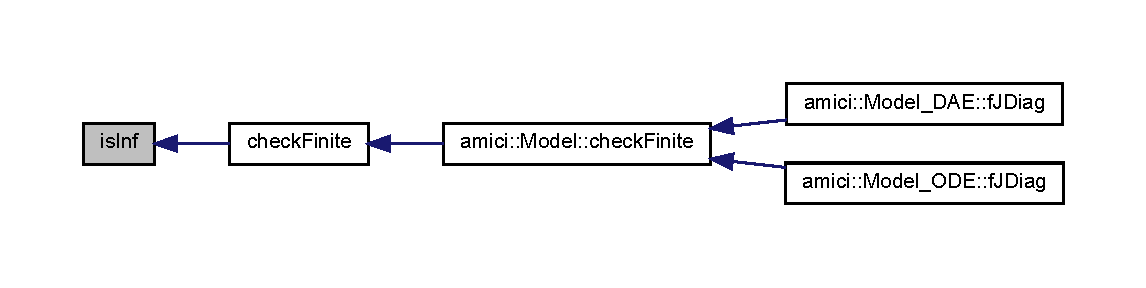
\includegraphics[width=350pt]{namespaceamici_a10c0a2eb43575a155a34f5bb280f7973_icgraph}
\end{center}
\end{figure}
\mbox{\Hypertarget{namespaceamici_ad41a03e53c2aaeeb82aad5791bf3ee28}\label{namespaceamici_ad41a03e53c2aaeeb82aad5791bf3ee28}} 
\index{amici@{amici}!get\+NaN@{get\+NaN}}
\index{get\+NaN@{get\+NaN}!amici@{amici}}
\paragraph{\texorpdfstring{get\+Na\+N()}{getNaN()}}
{\footnotesize\ttfamily double get\+NaN (\begin{DoxyParamCaption}{ }\end{DoxyParamCaption})}

function returning nan

\begin{DoxyReturn}{Returns}
NaN 
\end{DoxyReturn}


Definition at line 52 of file symbolic\+\_\+functions.\+cpp.

Here is the caller graph for this function\+:
\nopagebreak
\begin{figure}[H]
\begin{center}
\leavevmode
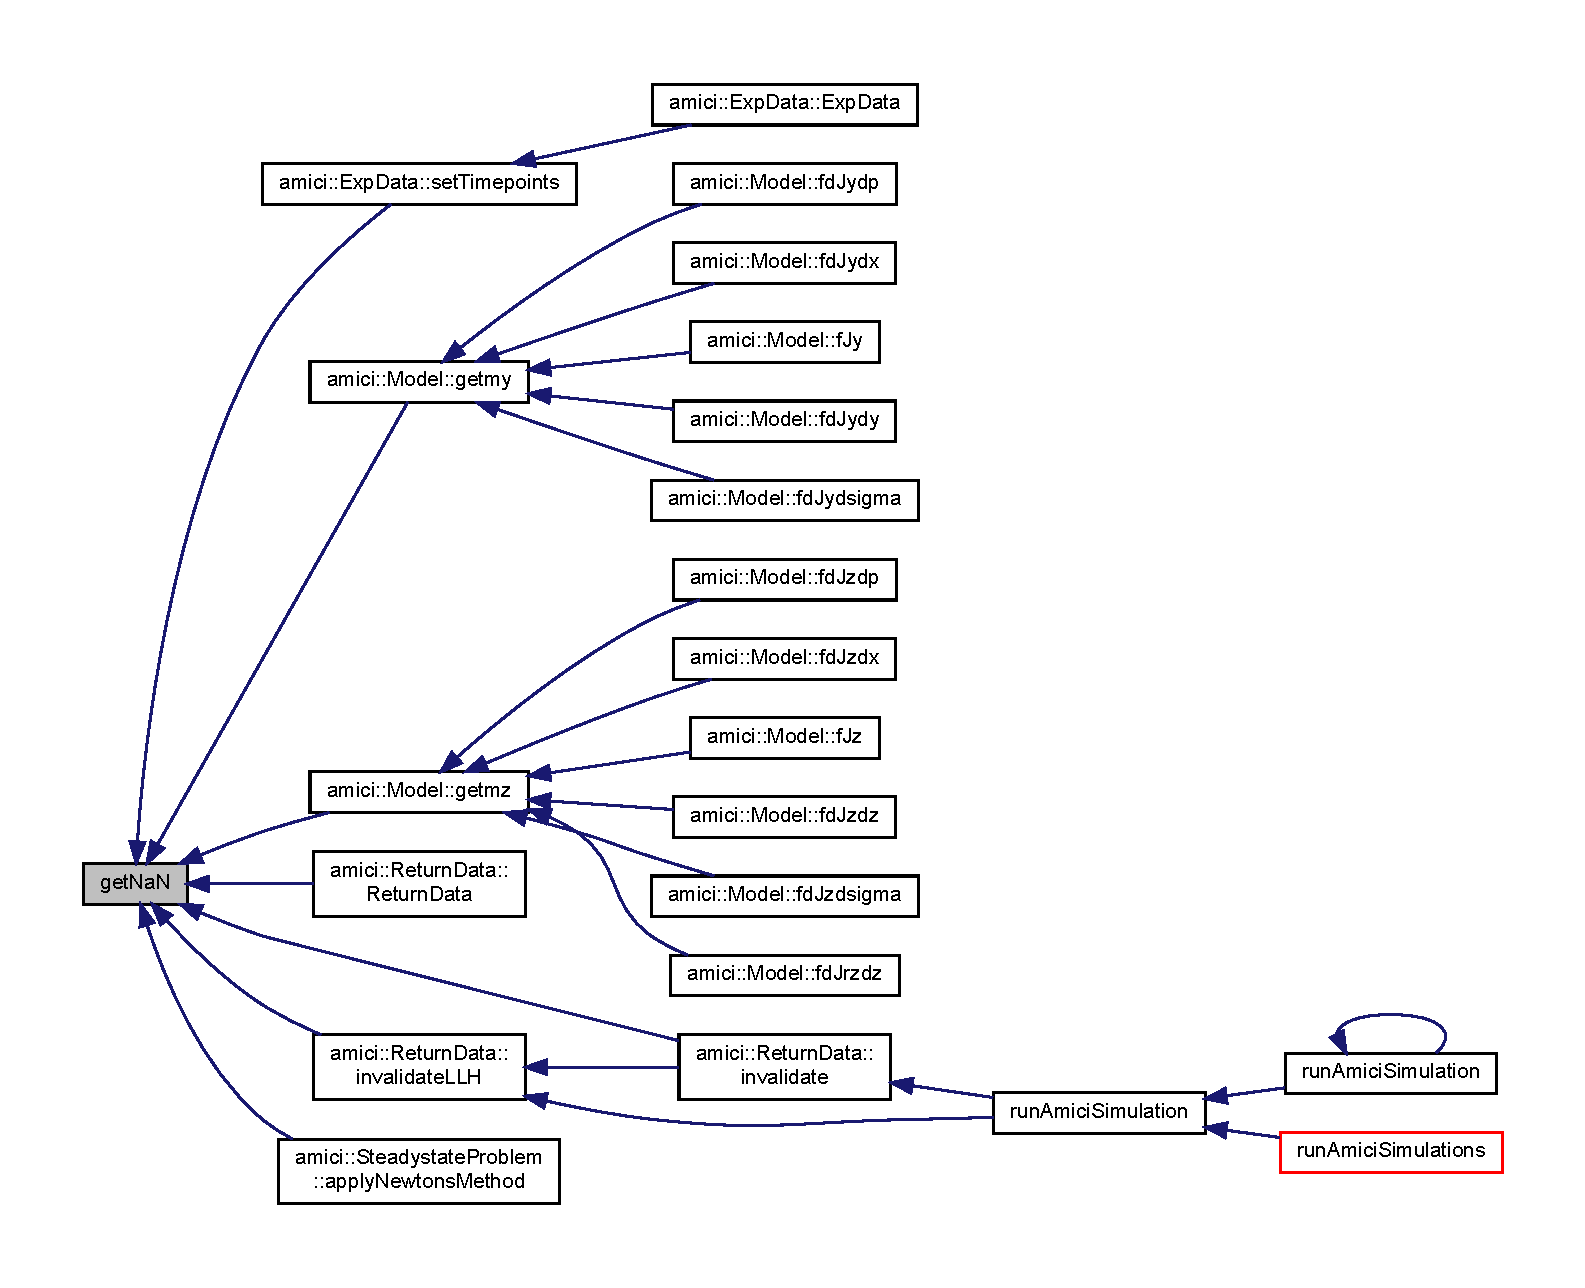
\includegraphics[width=350pt]{namespaceamici_ad41a03e53c2aaeeb82aad5791bf3ee28_icgraph}
\end{center}
\end{figure}
\mbox{\Hypertarget{namespaceamici_a8f3cba07aa75b7320ae8bd6c0aeac498}\label{namespaceamici_a8f3cba07aa75b7320ae8bd6c0aeac498}} 
\index{amici@{amici}!sign@{sign}}
\index{sign@{sign}!amici@{amici}}
\paragraph{\texorpdfstring{sign()}{sign()}}
{\footnotesize\ttfamily double sign (\begin{DoxyParamCaption}\item[{double}]{x }\end{DoxyParamCaption})}

c implementation of matlab function sign


\begin{DoxyParams}{Parameters}
{\em x} & argument \\
\hline
\end{DoxyParams}
\begin{DoxyReturn}{Returns}
0 
\end{DoxyReturn}


Definition at line 107 of file symbolic\+\_\+functions.\+cpp.

\mbox{\Hypertarget{namespaceamici_a34f81e95053af0b2d366f7ab636e603a}\label{namespaceamici_a34f81e95053af0b2d366f7ab636e603a}} 
\index{amici@{amici}!spline@{spline}}
\index{spline@{spline}!amici@{amici}}
\paragraph{\texorpdfstring{spline()}{spline()}\hspace{0.1cm}{\footnotesize\ttfamily [2/2]}}
{\footnotesize\ttfamily double spline (\begin{DoxyParamCaption}\item[{double}]{t,  }\item[{int}]{num,  }\item[{}]{... }\end{DoxyParamCaption})}

spline function, takes variable argument pairs (ti,pi) with {\ttfamily ti}\+: location of node i and {\ttfamily pi}\+: spline value at node i. the last two arguments are always {\ttfamily ss}\+: flag indicating whether slope at first node should be user defined and {\ttfamily dudt} user defined slope at first node. All arguments must be of type double.


\begin{DoxyParams}{Parameters}
{\em t} & point at which the spline should be evaluated \\
\hline
{\em num} & number of spline nodes\\
\hline
\end{DoxyParams}
\begin{DoxyReturn}{Returns}
spline(t) 
\end{DoxyReturn}


Definition at line 222 of file symbolic\+\_\+functions.\+cpp.

Here is the call graph for this function\+:
\nopagebreak
\begin{figure}[H]
\begin{center}
\leavevmode
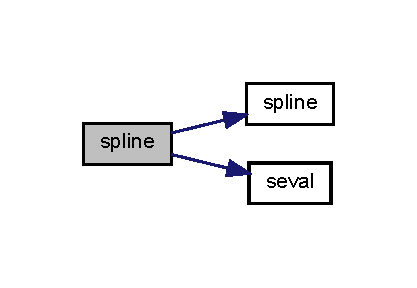
\includegraphics[width=200pt]{namespaceamici_a34f81e95053af0b2d366f7ab636e603a_cgraph}
\end{center}
\end{figure}
\mbox{\Hypertarget{namespaceamici_aa814c7e3b7d45495d0607f3af88027f6}\label{namespaceamici_aa814c7e3b7d45495d0607f3af88027f6}} 
\index{amici@{amici}!spline\+\_\+pos@{spline\+\_\+pos}}
\index{spline\+\_\+pos@{spline\+\_\+pos}!amici@{amici}}
\paragraph{\texorpdfstring{spline\+\_\+pos()}{spline\_pos()}}
{\footnotesize\ttfamily double spline\+\_\+pos (\begin{DoxyParamCaption}\item[{double}]{t,  }\item[{int}]{num,  }\item[{}]{... }\end{DoxyParamCaption})}

exponentiated spline function, takes variable argument pairs (ti,pi) with {\ttfamily ti}\+: location of node i and {\ttfamily pi}\+: spline value at node i. the last two arguments are always {\ttfamily ss}\+: flag indicating whether slope at first node should be user defined and {\ttfamily dudt} user defined slope at first node. All arguments must be of type double.


\begin{DoxyParams}{Parameters}
{\em t} & point at which the spline should be evaluated \\
\hline
{\em num} & number of spline nodes\\
\hline
\end{DoxyParams}
\begin{DoxyReturn}{Returns}
spline(t) 
\end{DoxyReturn}


Definition at line 273 of file symbolic\+\_\+functions.\+cpp.

Here is the call graph for this function\+:
\nopagebreak
\begin{figure}[H]
\begin{center}
\leavevmode
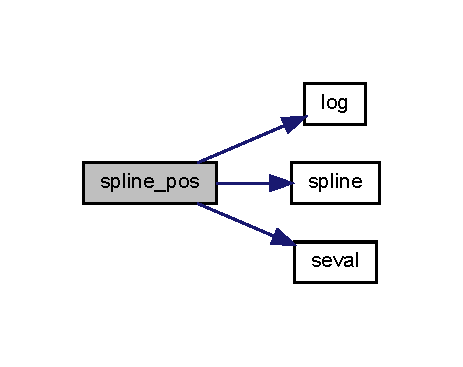
\includegraphics[width=222pt]{namespaceamici_aa814c7e3b7d45495d0607f3af88027f6_cgraph}
\end{center}
\end{figure}
\mbox{\Hypertarget{namespaceamici_ad4f5bcfd873d2945ed546194aa80c078}\label{namespaceamici_ad4f5bcfd873d2945ed546194aa80c078}} 
\index{amici@{amici}!Dspline@{Dspline}}
\index{Dspline@{Dspline}!amici@{amici}}
\paragraph{\texorpdfstring{Dspline()}{Dspline()}}
{\footnotesize\ttfamily double Dspline (\begin{DoxyParamCaption}\item[{int}]{id,  }\item[{double}]{t,  }\item[{int}]{num,  }\item[{}]{... }\end{DoxyParamCaption})}

derivation of a spline function, takes variable argument pairs (ti,pi) with {\ttfamily ti}\+: location of node i and {\ttfamily pi}\+: spline value at node i. the last two arguments are always {\ttfamily ss}\+: flag indicating whether slope at first node should be user defined and {\ttfamily dudt} user defined slope at first node. All arguments but id must be of type double.


\begin{DoxyParams}{Parameters}
{\em id} & index of node to which the derivative of the corresponding spline coefficient should be computed \\
\hline
{\em t} & point at which the spline should be evaluated \\
\hline
{\em num} & number of spline nodes\\
\hline
\end{DoxyParams}
\begin{DoxyReturn}{Returns}
dsplinedp(t) 
\end{DoxyReturn}


Definition at line 326 of file symbolic\+\_\+functions.\+cpp.

Here is the call graph for this function\+:
\nopagebreak
\begin{figure}[H]
\begin{center}
\leavevmode
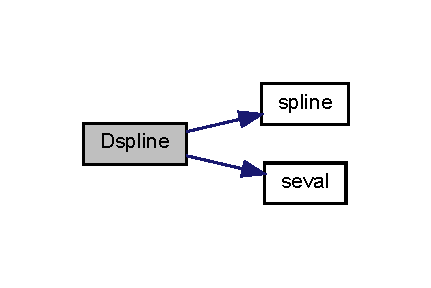
\includegraphics[width=207pt]{namespaceamici_ad4f5bcfd873d2945ed546194aa80c078_cgraph}
\end{center}
\end{figure}
\mbox{\Hypertarget{namespaceamici_a0d1393ca0920ddb402450709cc505f4f}\label{namespaceamici_a0d1393ca0920ddb402450709cc505f4f}} 
\index{amici@{amici}!Dspline\+\_\+pos@{Dspline\+\_\+pos}}
\index{Dspline\+\_\+pos@{Dspline\+\_\+pos}!amici@{amici}}
\paragraph{\texorpdfstring{Dspline\+\_\+pos()}{Dspline\_pos()}}
{\footnotesize\ttfamily double Dspline\+\_\+pos (\begin{DoxyParamCaption}\item[{int}]{id,  }\item[{double}]{t,  }\item[{int}]{num,  }\item[{}]{... }\end{DoxyParamCaption})}

derivation of an exponentiated spline function, takes variable argument pairs (ti,pi) with {\ttfamily ti}\+: location of node i and {\ttfamily pi}\+: spline value at node i. the last two arguments are always {\ttfamily ss}\+: flag indicating whether slope at first node should be user defined and {\ttfamily dudt} user defined slope at first node. All arguments but id must be of type double.


\begin{DoxyParams}{Parameters}
{\em id} & index of node to which the derivative of the corresponding spline coefficient should be computed \\
\hline
{\em t} & point at which the spline should be evaluated \\
\hline
{\em num} & number of spline nodes\\
\hline
\end{DoxyParams}
\begin{DoxyReturn}{Returns}
dsplinedp(t) 
\end{DoxyReturn}


Definition at line 382 of file symbolic\+\_\+functions.\+cpp.

Here is the call graph for this function\+:
\nopagebreak
\begin{figure}[H]
\begin{center}
\leavevmode
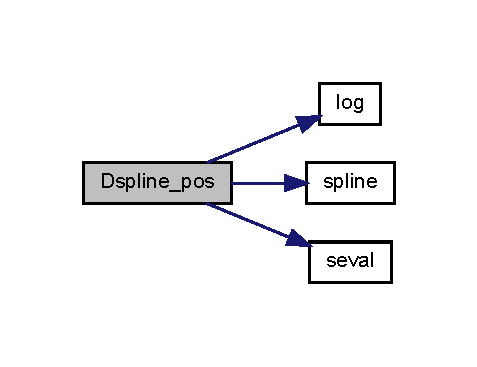
\includegraphics[width=229pt]{namespaceamici_a0d1393ca0920ddb402450709cc505f4f_cgraph}
\end{center}
\end{figure}
\mbox{\Hypertarget{namespaceamici_a5597be7f476a91dab4b6e948b548e14c}\label{namespaceamici_a5597be7f476a91dab4b6e948b548e14c}} 
\index{amici@{amici}!D\+Dspline@{D\+Dspline}}
\index{D\+Dspline@{D\+Dspline}!amici@{amici}}
\paragraph{\texorpdfstring{D\+Dspline()}{DDspline()}}
{\footnotesize\ttfamily double D\+Dspline (\begin{DoxyParamCaption}\item[{int}]{id1,  }\item[{int}]{id2,  }\item[{double}]{t,  }\item[{int}]{num,  }\item[{}]{... }\end{DoxyParamCaption})}

second derivation of a spline function, takes variable argument pairs (ti,pi) with {\ttfamily ti}\+: location of node i and {\ttfamily pi}\+: spline value at node i. the last two arguments are always {\ttfamily ss}\+: flag indicating whether slope at first node should be user defined and {\ttfamily dudt} user defined slope at first node. All arguments but id1 and id2 must be of type double.


\begin{DoxyParams}{Parameters}
{\em id1} & index of node to which the first derivative of the corresponding spline coefficient should be computed \\
\hline
{\em id2} & index of node to which the second derivative of the corresponding spline coefficient should be computed \\
\hline
{\em t} & point at which the spline should be evaluated \\
\hline
{\em num} & number of spline nodes\\
\hline
\end{DoxyParams}
\begin{DoxyReturn}{Returns}
ddspline(t) 
\end{DoxyReturn}


Definition at line 448 of file symbolic\+\_\+functions.\+cpp.

\mbox{\Hypertarget{namespaceamici_af6b968fef628d77ae0e9ad63e6e2558b}\label{namespaceamici_af6b968fef628d77ae0e9ad63e6e2558b}} 
\index{amici@{amici}!D\+Dspline\+\_\+pos@{D\+Dspline\+\_\+pos}}
\index{D\+Dspline\+\_\+pos@{D\+Dspline\+\_\+pos}!amici@{amici}}
\paragraph{\texorpdfstring{D\+Dspline\+\_\+pos()}{DDspline\_pos()}}
{\footnotesize\ttfamily double D\+Dspline\+\_\+pos (\begin{DoxyParamCaption}\item[{int}]{id1,  }\item[{int}]{id2,  }\item[{double}]{t,  }\item[{int}]{num,  }\item[{}]{... }\end{DoxyParamCaption})}

derivation of an exponentiated spline function, takes variable argument pairs (ti,pi) with {\ttfamily ti}\+: location of node i and {\ttfamily pi}\+: spline value at node i. the last two arguments are always {\ttfamily ss}\+: flag indicating whether slope at first node should be user defined and {\ttfamily dudt} user defined slope at first node. All arguments but id1 and id2 must be of type double.


\begin{DoxyParams}{Parameters}
{\em id1} & index of node to which the first derivative of the corresponding spline coefficient should be computed \\
\hline
{\em id2} & index of node to which the second derivative of the corresponding spline coefficient should be computed \\
\hline
{\em t} & point at which the spline should be evaluated \\
\hline
{\em num} & number of spline nodes\\
\hline
\end{DoxyParams}
\begin{DoxyReturn}{Returns}
ddspline(t) 
\end{DoxyReturn}


Definition at line 468 of file symbolic\+\_\+functions.\+cpp.

Here is the call graph for this function\+:
\nopagebreak
\begin{figure}[H]
\begin{center}
\leavevmode
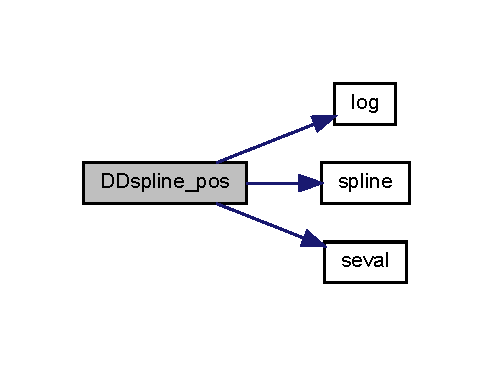
\includegraphics[width=236pt]{namespaceamici_af6b968fef628d77ae0e9ad63e6e2558b_cgraph}
\end{center}
\end{figure}
\mbox{\Hypertarget{namespaceamici_a9501315e2c79e5787a62c57c05ffe7c0}\label{namespaceamici_a9501315e2c79e5787a62c57c05ffe7c0}} 
\index{amici@{amici}!run\+Amici\+Simulation@{run\+Amici\+Simulation}}
\index{run\+Amici\+Simulation@{run\+Amici\+Simulation}!amici@{amici}}
\paragraph{\texorpdfstring{run\+Amici\+Simulation()}{runAmiciSimulation()}\hspace{0.1cm}{\footnotesize\ttfamily [2/2]}}
{\footnotesize\ttfamily def amici.\+run\+Amici\+Simulation (\begin{DoxyParamCaption}\item[{}]{model,  }\item[{}]{solver,  }\item[{}]{edata = {\ttfamily None} }\end{DoxyParamCaption})}


\begin{DoxyParams}{Parameters}
{\em model} & \mbox{\hyperlink{classamici_1_1_model}{Model}} instance \\
\hline
{\em solver} & \mbox{\hyperlink{classamici_1_1_solver}{Solver}} instance, must be generated from \mbox{\hyperlink{classamici_1_1_model_a61d5b19b2e4d5ffcc73a014d59494344}{Model.\+get\+Solver()}} \\
\hline
{\em edata} & \mbox{\hyperlink{classamici_1_1_exp_data}{Exp\+Data}} instance (optional)\\
\hline
\end{DoxyParams}
\begin{DoxyReturn}{Returns}
\mbox{\hyperlink{classamici_1_1_return_data}{Return\+Data}} object with simulation results 
\end{DoxyReturn}


Definition at line 93 of file \+\_\+\+\_\+init\+\_\+\+\_\+.\+py.

Here is the call graph for this function\+:
\nopagebreak
\begin{figure}[H]
\begin{center}
\leavevmode
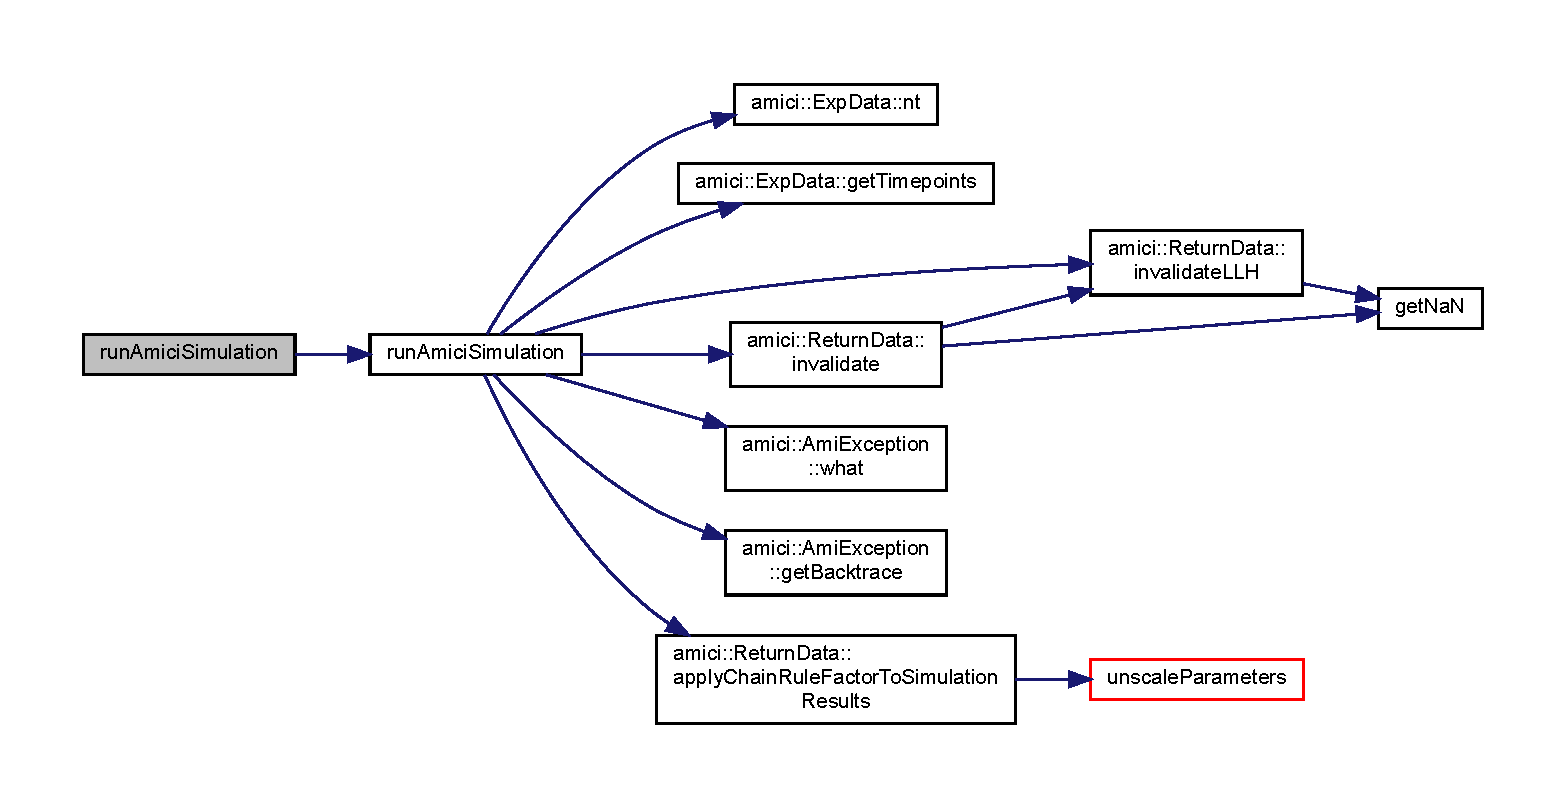
\includegraphics[width=350pt]{namespaceamici_a9501315e2c79e5787a62c57c05ffe7c0_cgraph}
\end{center}
\end{figure}
Here is the caller graph for this function\+:
\nopagebreak
\begin{figure}[H]
\begin{center}
\leavevmode
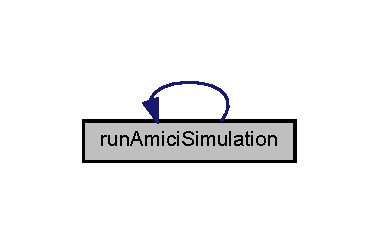
\includegraphics[width=182pt]{namespaceamici_a9501315e2c79e5787a62c57c05ffe7c0_icgraph}
\end{center}
\end{figure}
\mbox{\Hypertarget{namespaceamici_a16e08939fd8d9ac0e61164a1a94acb05}\label{namespaceamici_a16e08939fd8d9ac0e61164a1a94acb05}} 
\index{amici@{amici}!Exp\+Data@{Exp\+Data}}
\index{Exp\+Data@{Exp\+Data}!amici@{amici}}
\paragraph{\texorpdfstring{Exp\+Data()}{ExpData()}}
{\footnotesize\ttfamily def \mbox{\hyperlink{classamici_1_1_exp_data}{amici.\+Exp\+Data}} (\begin{DoxyParamCaption}\item[{}]{args }\end{DoxyParamCaption})}


\begin{DoxyParams}{Parameters}
{\em args} & arguments\\
\hline
\end{DoxyParams}
\begin{DoxyReturn}{Returns}
\mbox{\hyperlink{classamici_1_1_exp_data}{Exp\+Data}} Instance 
\end{DoxyReturn}


Definition at line 112 of file \+\_\+\+\_\+init\+\_\+\+\_\+.\+py.

Here is the caller graph for this function\+:
\nopagebreak
\begin{figure}[H]
\begin{center}
\leavevmode
\includegraphics[width=350pt]{namespaceamici_a16e08939fd8d9ac0e61164a1a94acb05_icgraph}
\end{center}
\end{figure}
\mbox{\Hypertarget{namespaceamici_a9fcd2221445c4966d12cd57b4b7f688e}\label{namespaceamici_a9fcd2221445c4966d12cd57b4b7f688e}} 
\index{amici@{amici}!run\+Amici\+Simulations@{run\+Amici\+Simulations}}
\index{run\+Amici\+Simulations@{run\+Amici\+Simulations}!amici@{amici}}
\paragraph{\texorpdfstring{run\+Amici\+Simulations()}{runAmiciSimulations()}\hspace{0.1cm}{\footnotesize\ttfamily [2/2]}}
{\footnotesize\ttfamily def amici.\+run\+Amici\+Simulations (\begin{DoxyParamCaption}\item[{}]{model,  }\item[{}]{solver,  }\item[{}]{edata\+\_\+list,  }\item[{}]{num\+\_\+threads = {\ttfamily 1} }\end{DoxyParamCaption})}


\begin{DoxyParams}{Parameters}
{\em model} & \mbox{\hyperlink{classamici_1_1_model}{Model}} instance \\
\hline
{\em solver} & \mbox{\hyperlink{classamici_1_1_solver}{Solver}} instance, must be generated from \mbox{\hyperlink{classamici_1_1_model_a61d5b19b2e4d5ffcc73a014d59494344}{Model.\+get\+Solver()}} \\
\hline
{\em edata\+\_\+list} & list of \mbox{\hyperlink{classamici_1_1_exp_data}{Exp\+Data}} instances \\
\hline
{\em num\+\_\+threads} & number of threads to use (only used if compiled with openmp)\\
\hline
\end{DoxyParams}
\begin{DoxyReturn}{Returns}
list of \mbox{\hyperlink{classamici_1_1_return_data}{Return\+Data}} objects with simulation results 
\end{DoxyReturn}


Definition at line 140 of file \+\_\+\+\_\+init\+\_\+\+\_\+.\+py.

Here is the call graph for this function\+:
\nopagebreak
\begin{figure}[H]
\begin{center}
\leavevmode
\includegraphics[width=350pt]{namespaceamici_a9fcd2221445c4966d12cd57b4b7f688e_cgraph}
\end{center}
\end{figure}
Here is the caller graph for this function\+:
\nopagebreak
\begin{figure}[H]
\begin{center}
\leavevmode
\includegraphics[width=187pt]{namespaceamici_a9fcd2221445c4966d12cd57b4b7f688e_icgraph}
\end{center}
\end{figure}
\mbox{\Hypertarget{namespaceamici_a204c68962100d0020a37392fef2e95e2}\label{namespaceamici_a204c68962100d0020a37392fef2e95e2}} 
\index{amici@{amici}!dbl2int@{dbl2int}}
\index{dbl2int@{dbl2int}!amici@{amici}}
\paragraph{\texorpdfstring{dbl2int()}{dbl2int()}}
{\footnotesize\ttfamily int dbl2int (\begin{DoxyParamCaption}\item[{const double}]{x }\end{DoxyParamCaption})}

conversion from double to int with checking for loss of data 
\begin{DoxyParams}{Parameters}
{\em x} & input \\
\hline
\end{DoxyParams}
\begin{DoxyReturn}{Returns}
int\+\_\+x casted value 
\end{DoxyReturn}


Definition at line 298 of file interface\+\_\+matlab.\+cpp.

Here is the caller graph for this function\+:
\nopagebreak
\begin{figure}[H]
\begin{center}
\leavevmode
\includegraphics[width=254pt]{namespaceamici_a204c68962100d0020a37392fef2e95e2_icgraph}
\end{center}
\end{figure}
\mbox{\Hypertarget{namespaceamici_a800e4c3e12f712281a4355e765402260}\label{namespaceamici_a800e4c3e12f712281a4355e765402260}} 
\index{amici@{amici}!amici\+\_\+blas\+C\+Blas\+Trans\+To\+Blas\+Trans@{amici\+\_\+blas\+C\+Blas\+Trans\+To\+Blas\+Trans}}
\index{amici\+\_\+blas\+C\+Blas\+Trans\+To\+Blas\+Trans@{amici\+\_\+blas\+C\+Blas\+Trans\+To\+Blas\+Trans}!amici@{amici}}
\paragraph{\texorpdfstring{amici\+\_\+blas\+C\+Blas\+Trans\+To\+Blas\+Trans()}{amici\_blasCBlasTransToBlasTrans()}}
{\footnotesize\ttfamily char amici\+::amici\+\_\+blas\+C\+Blas\+Trans\+To\+Blas\+Trans (\begin{DoxyParamCaption}\item[{\mbox{\hyperlink{namespaceamici_a0f0ec77c6c8f48d9c5cb50d54899afae}{B\+L\+A\+S\+Transpose}}}]{trans }\end{DoxyParamCaption})}

amici\+\_\+blas\+C\+Blas\+Trans\+To\+Blas\+Trans translates A\+M\+I\+C\+I\+\_\+\+B\+L\+A\+S\+\_\+\+T\+R\+A\+N\+S\+P\+O\+SE values to C\+Blas readable strings


\begin{DoxyParams}{Parameters}
{\em trans} & flag indicating transposition and complex conjugation\\
\hline
\end{DoxyParams}
\begin{DoxyReturn}{Returns}
cblastrans C\+Blas readable C\+H\+AR indicating transposition and complex conjugation 
\end{DoxyReturn}


Definition at line 52 of file interface\+\_\+matlab.\+cpp.

\mbox{\Hypertarget{namespaceamici_af8f91dbb6a395a9907c59dd92991ec18}\label{namespaceamici_af8f91dbb6a395a9907c59dd92991ec18}} 
\index{amici@{amici}!mx\+Array\+To\+Vector@{mx\+Array\+To\+Vector}}
\index{mx\+Array\+To\+Vector@{mx\+Array\+To\+Vector}!amici@{amici}}
\paragraph{\texorpdfstring{mx\+Array\+To\+Vector()}{mxArrayToVector()}}
{\footnotesize\ttfamily std\+::vector$<$\mbox{\hyperlink{namespaceamici_a1bdce28051d6a53868f7ccbf5f2c14a3}{realtype}}$>$ amici\+::mx\+Array\+To\+Vector (\begin{DoxyParamCaption}\item[{const mx\+Array $\ast$}]{array,  }\item[{int}]{length }\end{DoxyParamCaption})}

conversion from mx\+Array to vector$<$realtype$>$ 
\begin{DoxyParams}{Parameters}
{\em array} & Matlab array to create vector from \\
\hline
{\em length} & Number of elements in array \\
\hline
\end{DoxyParams}
\begin{DoxyReturn}{Returns}
std\+::vector with data from array 
\end{DoxyReturn}


Definition at line 166 of file interface\+\_\+matlab.\+cpp.

Here is the caller graph for this function\+:
\nopagebreak
\begin{figure}[H]
\begin{center}
\leavevmode
\includegraphics[width=350pt]{namespaceamici_af8f91dbb6a395a9907c59dd92991ec18_icgraph}
\end{center}
\end{figure}
\mbox{\Hypertarget{namespaceamici_a00a3387dd5fe07628c21a763aee28036}\label{namespaceamici_a00a3387dd5fe07628c21a763aee28036}} 
\index{amici@{amici}!get\+Value\+By\+Id@{get\+Value\+By\+Id}}
\index{get\+Value\+By\+Id@{get\+Value\+By\+Id}!amici@{amici}}
\paragraph{\texorpdfstring{get\+Value\+By\+Id()}{getValueById()}}
{\footnotesize\ttfamily \mbox{\hyperlink{namespaceamici_a1bdce28051d6a53868f7ccbf5f2c14a3}{realtype}} amici\+::get\+Value\+By\+Id (\begin{DoxyParamCaption}\item[{std\+::vector$<$ std\+::string $>$ const \&}]{ids,  }\item[{std\+::vector$<$ \mbox{\hyperlink{namespaceamici_a1bdce28051d6a53868f7ccbf5f2c14a3}{realtype}} $>$ const \&}]{values,  }\item[{std\+::string const \&}]{id,  }\item[{const char $\ast$}]{variable\+\_\+name,  }\item[{const char $\ast$}]{id\+\_\+name }\end{DoxyParamCaption})}


\begin{DoxyParams}{Parameters}
{\em ids} & vector of name/ids of (fixed)Parameters \\
\hline
{\em values} & values of the (fixed)Parameters \\
\hline
{\em id} & name/id to look for in the vector \\
\hline
{\em variable\+\_\+name} & string indicating what variable we are lookin at \\
\hline
{\em id\+\_\+name} & string indicating whether name or id was specified \\
\hline
\end{DoxyParams}
\begin{DoxyReturn}{Returns}
value of the selected parameter 
\end{DoxyReturn}


Definition at line 323 of file model.\+cpp.

Here is the caller graph for this function\+:
\nopagebreak
\begin{figure}[H]
\begin{center}
\leavevmode
\includegraphics[width=350pt]{namespaceamici_a00a3387dd5fe07628c21a763aee28036_icgraph}
\end{center}
\end{figure}
\mbox{\Hypertarget{namespaceamici_a939bff838284994570395c19eb40923d}\label{namespaceamici_a939bff838284994570395c19eb40923d}} 
\index{amici@{amici}!set\+Value\+By\+Id@{set\+Value\+By\+Id}}
\index{set\+Value\+By\+Id@{set\+Value\+By\+Id}!amici@{amici}}
\paragraph{\texorpdfstring{set\+Value\+By\+Id()}{setValueById()}}
{\footnotesize\ttfamily void amici\+::set\+Value\+By\+Id (\begin{DoxyParamCaption}\item[{std\+::vector$<$ std\+::string $>$ const \&}]{ids,  }\item[{std\+::vector$<$ \mbox{\hyperlink{namespaceamici_a1bdce28051d6a53868f7ccbf5f2c14a3}{realtype}} $>$ \&}]{values,  }\item[{\mbox{\hyperlink{namespaceamici_a1bdce28051d6a53868f7ccbf5f2c14a3}{realtype}}}]{value,  }\item[{std\+::string const \&}]{id,  }\item[{const char $\ast$}]{variable\+\_\+name,  }\item[{const char $\ast$}]{id\+\_\+name }\end{DoxyParamCaption})}


\begin{DoxyParams}{Parameters}
{\em ids} & vector of names/ids of (fixed)Parameters \\
\hline
{\em values} & values of the (fixed)Parameters \\
\hline
{\em value} & for the selected parameter \\
\hline
{\em id} & name/id to look for in the vector \\
\hline
{\em variable\+\_\+name} & string indicating what variable we are lookin at \\
\hline
{\em id\+\_\+name} & string indicating whether name or id was specified \\
\hline
\end{DoxyParams}


Definition at line 341 of file model.\+cpp.

Here is the caller graph for this function\+:
\nopagebreak
\begin{figure}[H]
\begin{center}
\leavevmode
\includegraphics[width=350pt]{namespaceamici_a939bff838284994570395c19eb40923d_icgraph}
\end{center}
\end{figure}
\mbox{\Hypertarget{namespaceamici_a0094499812e5edffce2ae9f379b11abb}\label{namespaceamici_a0094499812e5edffce2ae9f379b11abb}} 
\index{amici@{amici}!set\+Value\+By\+Id\+Regex@{set\+Value\+By\+Id\+Regex}}
\index{set\+Value\+By\+Id\+Regex@{set\+Value\+By\+Id\+Regex}!amici@{amici}}
\paragraph{\texorpdfstring{set\+Value\+By\+Id\+Regex()}{setValueByIdRegex()}}
{\footnotesize\ttfamily int amici\+::set\+Value\+By\+Id\+Regex (\begin{DoxyParamCaption}\item[{std\+::vector$<$ std\+::string $>$ const \&}]{ids,  }\item[{std\+::vector$<$ \mbox{\hyperlink{namespaceamici_a1bdce28051d6a53868f7ccbf5f2c14a3}{realtype}} $>$ \&}]{values,  }\item[{\mbox{\hyperlink{namespaceamici_a1bdce28051d6a53868f7ccbf5f2c14a3}{realtype}}}]{value,  }\item[{std\+::string const \&}]{regex,  }\item[{const char $\ast$}]{variable\+\_\+name,  }\item[{const char $\ast$}]{id\+\_\+name }\end{DoxyParamCaption})}


\begin{DoxyParams}{Parameters}
{\em ids} & vector of names/ids of (fixed)Parameters \\
\hline
{\em values} & values of the (fixed)Parameters \\
\hline
{\em value} & for the selected parameter \\
\hline
{\em regex} & string according to which names/ids are to be matched \\
\hline
{\em variable\+\_\+name} & string indicating what variable we are lookin at \\
\hline
{\em id\+\_\+name} & string indicating whether name or id was specified \\
\hline
\end{DoxyParams}
\begin{DoxyReturn}{Returns}
number of matched names/ids 
\end{DoxyReturn}


Definition at line 360 of file model.\+cpp.

Here is the caller graph for this function\+:
\nopagebreak
\begin{figure}[H]
\begin{center}
\leavevmode
\includegraphics[width=350pt]{namespaceamici_a0094499812e5edffce2ae9f379b11abb_icgraph}
\end{center}
\end{figure}


\subsubsection{Variable Documentation}
\mbox{\Hypertarget{namespaceamici_a19eefc037cc960b013cc0b724e5292b7}\label{namespaceamici_a19eefc037cc960b013cc0b724e5292b7}} 
\index{amici@{amici}!err\+Msg\+Id\+And\+Txt@{err\+Msg\+Id\+And\+Txt}}
\index{err\+Msg\+Id\+And\+Txt@{err\+Msg\+Id\+And\+Txt}!amici@{amici}}
\paragraph{\texorpdfstring{err\+Msg\+Id\+And\+Txt}{errMsgIdAndTxt}}
{\footnotesize\ttfamily \mbox{\hyperlink{namespaceamici_a02384ab9af881494db3ed32cd6ecdcc0}{msg\+Id\+And\+Txt\+Fp}} err\+Msg\+Id\+And\+Txt = \&\mbox{\hyperlink{namespaceamici_ade28c6a7f1b5aee40bb2453fb61b4024}{print\+Err\+Msg\+Id\+And\+Txt}}}

err\+Msg\+Id\+And\+Txt is a function pointer for print\+Err\+Msg\+Id\+And\+Txt 

Definition at line 37 of file amici.\+cpp.

\mbox{\Hypertarget{namespaceamici_adb95b29229e987b4b0a55ade25961688}\label{namespaceamici_adb95b29229e987b4b0a55ade25961688}} 
\index{amici@{amici}!warn\+Msg\+Id\+And\+Txt@{warn\+Msg\+Id\+And\+Txt}}
\index{warn\+Msg\+Id\+And\+Txt@{warn\+Msg\+Id\+And\+Txt}!amici@{amici}}
\paragraph{\texorpdfstring{warn\+Msg\+Id\+And\+Txt}{warnMsgIdAndTxt}}
{\footnotesize\ttfamily \mbox{\hyperlink{namespaceamici_a02384ab9af881494db3ed32cd6ecdcc0}{msg\+Id\+And\+Txt\+Fp}} warn\+Msg\+Id\+And\+Txt = \&\mbox{\hyperlink{namespaceamici_a14122f73594a970df27bfcb8fa0db35d}{print\+Warn\+Msg\+Id\+And\+Txt}}}

warn\+Msg\+Id\+And\+Txt is a function pointer for print\+Warn\+Msg\+Id\+And\+Txt 

Definition at line 13 of file model\+\_\+dae.\+h.

\mbox{\Hypertarget{namespaceamici_ad172e8d1a294401209781f9aeaa77410}\label{namespaceamici_ad172e8d1a294401209781f9aeaa77410}} 
\index{amici@{amici}!pi@{pi}}
\index{pi@{pi}!amici@{amici}}
\paragraph{\texorpdfstring{pi}{pi}}
{\footnotesize\ttfamily constexpr double pi = 3.\+14159265358979323846}

MS definition of PI and other constants 

Definition at line 13 of file defines.\+h.

\mbox{\Hypertarget{namespaceamici_a6b3f3dfe4601baaa0bf0a02b9a01a896}\label{namespaceamici_a6b3f3dfe4601baaa0bf0a02b9a01a896}} 
\index{amici@{amici}!amici\+\_\+path@{amici\+\_\+path}}
\index{amici\+\_\+path@{amici\+\_\+path}!amici@{amici}}
\paragraph{\texorpdfstring{amici\+\_\+path}{amici\_path}}
{\footnotesize\ttfamily amici\+\_\+path}

{\bfseries Initial value\+:}
\begin{DoxyCode}
1 =  os.path.abspath(os.path.join(
2         os.path.dirname(\_\_file\_\_), \textcolor{stringliteral}{'..'}, \textcolor{stringliteral}{'..'}))
\end{DoxyCode}


Definition at line 55 of file \+\_\+\+\_\+init\+\_\+\+\_\+.\+py.


\hypertarget{namespaceamici_1_1ode__export}{}\subsection{amici.\+ode\+\_\+export Namespace Reference}
\label{namespaceamici_1_1ode__export}\index{amici.\+ode\+\_\+export@{amici.\+ode\+\_\+export}}


The C++ O\+DE export module for python.  


\subsubsection*{Classes}
\begin{DoxyCompactItemize}
\item 
class \mbox{\hyperlink{classamici_1_1ode__export_1_1_constant}{Constant}}
\begin{DoxyCompactList}\small\item\em A \mbox{\hyperlink{classamici_1_1ode__export_1_1_constant}{Constant}} is a fixed variable in the model with respect to which sensitivites cannot be computed, abbreviated by {\ttfamily k} \end{DoxyCompactList}\item 
class \mbox{\hyperlink{classamici_1_1ode__export_1_1_expression}{Expression}}
\begin{DoxyCompactList}\small\item\em An Expressions is a recurring elements in symbolic formulas. \end{DoxyCompactList}\item 
class \mbox{\hyperlink{classamici_1_1ode__export_1_1_log_likelihood}{Log\+Likelihood}}
\begin{DoxyCompactList}\small\item\em A \mbox{\hyperlink{classamici_1_1ode__export_1_1_log_likelihood}{Log\+Likelihood}} defines the distance between measurements and experiments for a particular observable. \end{DoxyCompactList}\item 
class \mbox{\hyperlink{classamici_1_1ode__export_1_1_model_quantity}{Model\+Quantity}}
\begin{DoxyCompactList}\small\item\em Base class for model components. \end{DoxyCompactList}\item 
class \mbox{\hyperlink{classamici_1_1ode__export_1_1_observable}{Observable}}
\begin{DoxyCompactList}\small\item\em An \mbox{\hyperlink{classamici_1_1ode__export_1_1_observable}{Observable}} links model simulations to experimental measurements, abbreviated by {\ttfamily y} \end{DoxyCompactList}\item 
class \mbox{\hyperlink{classamici_1_1ode__export_1_1_o_d_e_exporter}{O\+D\+E\+Exporter}}
\begin{DoxyCompactList}\small\item\em The \mbox{\hyperlink{classamici_1_1ode__export_1_1_o_d_e_exporter}{O\+D\+E\+Exporter}} class generates A\+M\+I\+CI C++ files for O\+DE model as defined in symbolic expressions. \end{DoxyCompactList}\item 
class \mbox{\hyperlink{classamici_1_1ode__export_1_1_o_d_e_model}{O\+D\+E\+Model}}
\begin{DoxyCompactList}\small\item\em An \mbox{\hyperlink{classamici_1_1ode__export_1_1_o_d_e_model}{O\+D\+E\+Model}} defines an Ordinay Differential Equation as set of Model\+Quantities. \end{DoxyCompactList}\item 
class \mbox{\hyperlink{classamici_1_1ode__export_1_1_parameter}{Parameter}}
\begin{DoxyCompactList}\small\item\em A \mbox{\hyperlink{classamici_1_1ode__export_1_1_parameter}{Parameter}} is a free variable in the model with respect to which sensitivites may be computed, abbreviated by {\ttfamily p} \end{DoxyCompactList}\item 
class \mbox{\hyperlink{classamici_1_1ode__export_1_1_sigma_y}{SigmaY}}
\begin{DoxyCompactList}\small\item\em A Standard Deviation \mbox{\hyperlink{classamici_1_1ode__export_1_1_sigma_y}{SigmaY}} rescales the distance between simulations and measurements when computing residuals, abbreviated by {\ttfamily sigmay} \end{DoxyCompactList}\item 
class \mbox{\hyperlink{classamici_1_1ode__export_1_1_state}{State}}
\begin{DoxyCompactList}\small\item\em A \mbox{\hyperlink{classamici_1_1ode__export_1_1_state}{State}} variable defines an entity that evolves with time according to the provided time derivative, abbreviated by {\ttfamily x} \end{DoxyCompactList}\item 
class \mbox{\hyperlink{classamici_1_1ode__export_1_1_template_amici}{Template\+Amici}}
\begin{DoxyCompactList}\small\item\em Template format used in A\+M\+I\+CI (see string.\+template for more details). \end{DoxyCompactList}\end{DoxyCompactItemize}
\subsubsection*{Functions}
\begin{DoxyCompactItemize}
\item 
def \mbox{\hyperlink{namespaceamici_1_1ode__export_a365aaf8b78bb2db9c94b1a8087d60a16}{var\+\_\+in\+\_\+function\+\_\+signature}} (name, varname)
\begin{DoxyCompactList}\small\item\em Checks if the values for a symbolic variable is passed in the signature of a function. \end{DoxyCompactList}\item 
def \mbox{\hyperlink{namespaceamici_1_1ode__export_aed240175cce2aa528fe24d1486c52559}{get\+Symbolic\+Diagonal}} (matrix)
\begin{DoxyCompactList}\small\item\em Get symbolic matrix with diagonal of matrix {\ttfamily matrix}. \end{DoxyCompactList}\item 
def \mbox{\hyperlink{namespaceamici_1_1ode__export_af4b013340d08cdef3247601d2bf0b62f}{apply\+Template}} (source\+File, target\+File, template\+Data)
\begin{DoxyCompactList}\small\item\em Load source file, apply template substitution as provided in template\+Data and save as target\+File. \end{DoxyCompactList}\item 
def \mbox{\hyperlink{namespaceamici_1_1ode__export_af0bfa7839b41792994b1add20b86cf8e}{sanitize\+\_\+basic\+\_\+sympy}} (basic)
\begin{DoxyCompactList}\small\item\em Strips pysb info from the sympy.\+Basic object. \end{DoxyCompactList}\end{DoxyCompactItemize}
\subsubsection*{Variables}
\begin{DoxyCompactItemize}
\item 
\mbox{\Hypertarget{namespaceamici_1_1ode__export_ab2b7137f89298a92623c1c65239eaef2}\label{namespaceamici_1_1ode__export_ab2b7137f89298a92623c1c65239eaef2}} 
\mbox{\hyperlink{namespaceamici_1_1ode__export_ab2b7137f89298a92623c1c65239eaef2}{pysb}} = None
\begin{DoxyCompactList}\small\item\em pysb import dummy \end{DoxyCompactList}\item 
dictionary \mbox{\hyperlink{namespaceamici_1_1ode__export_ac310aa598d85b31cc0acea80dcc3c083}{functions}}
\begin{DoxyCompactList}\small\item\em prototype for generated C++ functions, keys are the names of functions \end{DoxyCompactList}\item 
list \mbox{\hyperlink{namespaceamici_1_1ode__export_aa54a407fede674f20bf6ba67fe27177d}{sparse\+\_\+functions}}
\begin{DoxyCompactList}\small\item\em list of sparse functions \end{DoxyCompactList}\item 
list \mbox{\hyperlink{namespaceamici_1_1ode__export_aceecbd374d0134e5683a78e882c3977d}{sensi\+\_\+functions}}
\begin{DoxyCompactList}\small\item\em list of sensitivity functions \end{DoxyCompactList}\item 
list \mbox{\hyperlink{namespaceamici_1_1ode__export_a8a1eabf284172d18098ca450147d94ca}{multiobs\+\_\+functions}}
\begin{DoxyCompactList}\small\item\em list of multiobs functions \end{DoxyCompactList}\item 
dictionary \mbox{\hyperlink{namespaceamici_1_1ode__export_a8faf4dadc2544b8b5dd81c443f66f958}{symbol\+\_\+to\+\_\+type}}
\begin{DoxyCompactList}\small\item\em indicates which type some attributes in \mbox{\hyperlink{classamici_1_1ode__export_1_1_o_d_e_model}{O\+D\+E\+Model}} should have \end{DoxyCompactList}\end{DoxyCompactItemize}


\subsubsection{Detailed Description}
!/usr/bin/env python3 

\subsubsection{Function Documentation}
\mbox{\Hypertarget{namespaceamici_1_1ode__export_a365aaf8b78bb2db9c94b1a8087d60a16}\label{namespaceamici_1_1ode__export_a365aaf8b78bb2db9c94b1a8087d60a16}} 
\index{amici\+::ode\+\_\+export@{amici\+::ode\+\_\+export}!var\+\_\+in\+\_\+function\+\_\+signature@{var\+\_\+in\+\_\+function\+\_\+signature}}
\index{var\+\_\+in\+\_\+function\+\_\+signature@{var\+\_\+in\+\_\+function\+\_\+signature}!amici\+::ode\+\_\+export@{amici\+::ode\+\_\+export}}
\paragraph{\texorpdfstring{var\+\_\+in\+\_\+function\+\_\+signature()}{var\_in\_function\_signature()}}
{\footnotesize\ttfamily def amici.\+ode\+\_\+export.\+var\+\_\+in\+\_\+function\+\_\+signature (\begin{DoxyParamCaption}\item[{}]{name,  }\item[{}]{varname }\end{DoxyParamCaption})}


\begin{DoxyParams}{Parameters}
{\em name} & name of the function ~\newline
{\bfseries Type}\+: str\\
\hline
{\em varname} & name of the symbolic variable ~\newline
{\bfseries Type}\+: str\\
\hline
\end{DoxyParams}
\begin{DoxyReturn}{Returns}

\end{DoxyReturn}


Definition at line 277 of file ode\+\_\+export.\+py.

Here is the caller graph for this function\+:
\nopagebreak
\begin{figure}[H]
\begin{center}
\leavevmode
\includegraphics[width=350pt]{namespaceamici_1_1ode__export_a365aaf8b78bb2db9c94b1a8087d60a16_icgraph}
\end{center}
\end{figure}
\mbox{\Hypertarget{namespaceamici_1_1ode__export_aed240175cce2aa528fe24d1486c52559}\label{namespaceamici_1_1ode__export_aed240175cce2aa528fe24d1486c52559}} 
\index{amici\+::ode\+\_\+export@{amici\+::ode\+\_\+export}!get\+Symbolic\+Diagonal@{get\+Symbolic\+Diagonal}}
\index{get\+Symbolic\+Diagonal@{get\+Symbolic\+Diagonal}!amici\+::ode\+\_\+export@{amici\+::ode\+\_\+export}}
\paragraph{\texorpdfstring{get\+Symbolic\+Diagonal()}{getSymbolicDiagonal()}}
{\footnotesize\ttfamily def amici.\+ode\+\_\+export.\+get\+Symbolic\+Diagonal (\begin{DoxyParamCaption}\item[{}]{matrix }\end{DoxyParamCaption})}


\begin{DoxyParams}{Parameters}
{\em matrix} & Matrix from which to return the diagonal ~\newline
{\bfseries Type}\+: symengine.\+Dense\+Matrix\\
\hline
\end{DoxyParams}
\begin{DoxyReturn}{Returns}
A Symbolic matrix with the diagonal of {\ttfamily matrix}.
\end{DoxyReturn}

\begin{DoxyExceptions}{Exceptions}
{\em Exception} & The provided matrix was not square \\
\hline
\end{DoxyExceptions}


Definition at line 2235 of file ode\+\_\+export.\+py.

Here is the caller graph for this function\+:
\nopagebreak
\begin{figure}[H]
\begin{center}
\leavevmode
\includegraphics[width=350pt]{namespaceamici_1_1ode__export_aed240175cce2aa528fe24d1486c52559_icgraph}
\end{center}
\end{figure}
\mbox{\Hypertarget{namespaceamici_1_1ode__export_af4b013340d08cdef3247601d2bf0b62f}\label{namespaceamici_1_1ode__export_af4b013340d08cdef3247601d2bf0b62f}} 
\index{amici\+::ode\+\_\+export@{amici\+::ode\+\_\+export}!apply\+Template@{apply\+Template}}
\index{apply\+Template@{apply\+Template}!amici\+::ode\+\_\+export@{amici\+::ode\+\_\+export}}
\paragraph{\texorpdfstring{apply\+Template()}{applyTemplate()}}
{\footnotesize\ttfamily def amici.\+ode\+\_\+export.\+apply\+Template (\begin{DoxyParamCaption}\item[{}]{source\+File,  }\item[{}]{target\+File,  }\item[{}]{template\+Data }\end{DoxyParamCaption})}


\begin{DoxyParams}{Parameters}
{\em source\+File} & relative or absolute path to template file ~\newline
{\bfseries Type}\+: str\\
\hline
{\em target\+File} & relative or absolute path to output file ~\newline
{\bfseries Type}\+: str\\
\hline
{\em template\+Data} & template keywords to substitute (key is template variable without \mbox{\hyperlink{classamici_1_1ode__export_1_1_template_amici_aacf4e58be14eef37272a71c004bc3f58}{Template\+Amici.\+delimiter}}) ~\newline
{\bfseries Type}\+: dict\\
\hline
\end{DoxyParams}
\begin{DoxyReturn}{Returns}

\end{DoxyReturn}


Definition at line 2271 of file ode\+\_\+export.\+py.

Here is the caller graph for this function\+:
\nopagebreak
\begin{figure}[H]
\begin{center}
\leavevmode
\includegraphics[width=350pt]{namespaceamici_1_1ode__export_af4b013340d08cdef3247601d2bf0b62f_icgraph}
\end{center}
\end{figure}
\mbox{\Hypertarget{namespaceamici_1_1ode__export_af0bfa7839b41792994b1add20b86cf8e}\label{namespaceamici_1_1ode__export_af0bfa7839b41792994b1add20b86cf8e}} 
\index{amici\+::ode\+\_\+export@{amici\+::ode\+\_\+export}!sanitize\+\_\+basic\+\_\+sympy@{sanitize\+\_\+basic\+\_\+sympy}}
\index{sanitize\+\_\+basic\+\_\+sympy@{sanitize\+\_\+basic\+\_\+sympy}!amici\+::ode\+\_\+export@{amici\+::ode\+\_\+export}}
\paragraph{\texorpdfstring{sanitize\+\_\+basic\+\_\+sympy()}{sanitize\_basic\_sympy()}}
{\footnotesize\ttfamily def amici.\+ode\+\_\+export.\+sanitize\+\_\+basic\+\_\+sympy (\begin{DoxyParamCaption}\item[{}]{basic }\end{DoxyParamCaption})}


\begin{DoxyParams}{Parameters}
{\em basic} & symbolic expression ~\newline
{\bfseries Type}\+: sympy.\+Basic\\
\hline
\end{DoxyParams}
\begin{DoxyReturn}{Returns}
sanitized sympy.\+Basic 
\end{DoxyReturn}


Definition at line 2290 of file ode\+\_\+export.\+py.

Here is the caller graph for this function\+:
\nopagebreak
\begin{figure}[H]
\begin{center}
\leavevmode
\includegraphics[width=350pt]{namespaceamici_1_1ode__export_af0bfa7839b41792994b1add20b86cf8e_icgraph}
\end{center}
\end{figure}


\subsubsection{Variable Documentation}
\mbox{\Hypertarget{namespaceamici_1_1ode__export_ac310aa598d85b31cc0acea80dcc3c083}\label{namespaceamici_1_1ode__export_ac310aa598d85b31cc0acea80dcc3c083}} 
\index{amici\+::ode\+\_\+export@{amici\+::ode\+\_\+export}!functions@{functions}}
\index{functions@{functions}!amici\+::ode\+\_\+export@{amici\+::ode\+\_\+export}}
\paragraph{\texorpdfstring{functions}{functions}}
{\footnotesize\ttfamily dictionary functions}

signature\+: defines the argument part of the function signature, input variables should have a const flag

assume\+\_\+pow\+\_\+positivity\+: identifies the functions on which assume\+\_\+pow\+\_\+positivity will have an effect when specified during model generation. generally these are functions that are used for solving the O\+DE, where negative values may negatively affect convergence of the integration algorithm

sparse\+: specifies whether the result of this function will be stored in sparse format. sparse format means that the function will only return an array of nonzero values and not a full matrix. 

Definition at line 40 of file ode\+\_\+export.\+py.

\mbox{\Hypertarget{namespaceamici_1_1ode__export_aa54a407fede674f20bf6ba67fe27177d}\label{namespaceamici_1_1ode__export_aa54a407fede674f20bf6ba67fe27177d}} 
\index{amici\+::ode\+\_\+export@{amici\+::ode\+\_\+export}!sparse\+\_\+functions@{sparse\+\_\+functions}}
\index{sparse\+\_\+functions@{sparse\+\_\+functions}!amici\+::ode\+\_\+export@{amici\+::ode\+\_\+export}}
\paragraph{\texorpdfstring{sparse\+\_\+functions}{sparse\_functions}}
{\footnotesize\ttfamily list sparse\+\_\+functions}

{\bfseries Initial value\+:}
\begin{DoxyCode}
1 =  [
2     function \textcolor{keywordflow}{for} function \textcolor{keywordflow}{in} functions
3     \textcolor{keywordflow}{if} \textcolor{stringliteral}{'sparse'} \textcolor{keywordflow}{in} functions[function]
4     \textcolor{keywordflow}{and} functions[function][\textcolor{stringliteral}{'sparse'}]
5 ]
\end{DoxyCode}


Definition at line 246 of file ode\+\_\+export.\+py.

\mbox{\Hypertarget{namespaceamici_1_1ode__export_aceecbd374d0134e5683a78e882c3977d}\label{namespaceamici_1_1ode__export_aceecbd374d0134e5683a78e882c3977d}} 
\index{amici\+::ode\+\_\+export@{amici\+::ode\+\_\+export}!sensi\+\_\+functions@{sensi\+\_\+functions}}
\index{sensi\+\_\+functions@{sensi\+\_\+functions}!amici\+::ode\+\_\+export@{amici\+::ode\+\_\+export}}
\paragraph{\texorpdfstring{sensi\+\_\+functions}{sensi\_functions}}
{\footnotesize\ttfamily list sensi\+\_\+functions}

{\bfseries Initial value\+:}
\begin{DoxyCode}
1 =  [
2     function \textcolor{keywordflow}{for} function \textcolor{keywordflow}{in} functions
3     \textcolor{keywordflow}{if} \textcolor{stringliteral}{'const int ip'} \textcolor{keywordflow}{in} functions[function][\textcolor{stringliteral}{'signature'}]
4     \textcolor{keywordflow}{and} function \textcolor{keywordflow}{is} \textcolor{keywordflow}{not} \textcolor{stringliteral}{'sxdot'}
5 ]
\end{DoxyCode}


Definition at line 252 of file ode\+\_\+export.\+py.

\mbox{\Hypertarget{namespaceamici_1_1ode__export_a8a1eabf284172d18098ca450147d94ca}\label{namespaceamici_1_1ode__export_a8a1eabf284172d18098ca450147d94ca}} 
\index{amici\+::ode\+\_\+export@{amici\+::ode\+\_\+export}!multiobs\+\_\+functions@{multiobs\+\_\+functions}}
\index{multiobs\+\_\+functions@{multiobs\+\_\+functions}!amici\+::ode\+\_\+export@{amici\+::ode\+\_\+export}}
\paragraph{\texorpdfstring{multiobs\+\_\+functions}{multiobs\_functions}}
{\footnotesize\ttfamily list multiobs\+\_\+functions}

{\bfseries Initial value\+:}
\begin{DoxyCode}
1 =  [
2     function \textcolor{keywordflow}{for} function \textcolor{keywordflow}{in} functions
3     \textcolor{keywordflow}{if} \textcolor{stringliteral}{'const int iy'} \textcolor{keywordflow}{in} functions[function][\textcolor{stringliteral}{'signature'}]
4 ]
\end{DoxyCode}


Definition at line 258 of file ode\+\_\+export.\+py.

\mbox{\Hypertarget{namespaceamici_1_1ode__export_a8faf4dadc2544b8b5dd81c443f66f958}\label{namespaceamici_1_1ode__export_a8faf4dadc2544b8b5dd81c443f66f958}} 
\index{amici\+::ode\+\_\+export@{amici\+::ode\+\_\+export}!symbol\+\_\+to\+\_\+type@{symbol\+\_\+to\+\_\+type}}
\index{symbol\+\_\+to\+\_\+type@{symbol\+\_\+to\+\_\+type}!amici\+::ode\+\_\+export@{amici\+::ode\+\_\+export}}
\paragraph{\texorpdfstring{symbol\+\_\+to\+\_\+type}{symbol\_to\_type}}
{\footnotesize\ttfamily dictionary symbol\+\_\+to\+\_\+type}

{\bfseries Initial value\+:}
\begin{DoxyCode}
1 =  \{
2     \textcolor{stringliteral}{'species'}: State,
3     \textcolor{stringliteral}{'parameter'}: Parameter,
4     \textcolor{stringliteral}{'fixed\_parameter'}: Constant,
5     \textcolor{stringliteral}{'observable'}: Observable,
6     \textcolor{stringliteral}{'sigmay'}: SigmaY,
7     \textcolor{stringliteral}{'llhy'}: LogLikelihood,
8     \textcolor{stringliteral}{'expression'}: Expression,
9 \}
\end{DoxyCode}


Definition at line 549 of file ode\+\_\+export.\+py.


\hypertarget{namespaceamici_1_1plotting}{}\subsection{amici.\+plotting Namespace Reference}
\label{namespaceamici_1_1plotting}\index{amici.\+plotting@{amici.\+plotting}}


Plotting related functions.  


\subsubsection*{Functions}
\begin{DoxyCompactItemize}
\item 
def \mbox{\hyperlink{namespaceamici_1_1plotting_acd5cb5084b075aa388dc43b9bb3c89a6}{plot\+State\+Trajectories}} (rdata, state\+\_\+indices=None, ax=None)
\begin{DoxyCompactList}\small\item\em Plot state trajectories. \end{DoxyCompactList}\item 
def \mbox{\hyperlink{namespaceamici_1_1plotting_aad83ff2d2783fe975309f8d129ad0f3b}{plot\+Observable\+Trajectories}} (rdata, observable\+\_\+indices=None, ax=None)
\begin{DoxyCompactList}\small\item\em Plot observable trajectories. \end{DoxyCompactList}\end{DoxyCompactItemize}


\subsubsection{Function Documentation}
\mbox{\Hypertarget{namespaceamici_1_1plotting_acd5cb5084b075aa388dc43b9bb3c89a6}\label{namespaceamici_1_1plotting_acd5cb5084b075aa388dc43b9bb3c89a6}} 
\index{amici\+::plotting@{amici\+::plotting}!plot\+State\+Trajectories@{plot\+State\+Trajectories}}
\index{plot\+State\+Trajectories@{plot\+State\+Trajectories}!amici\+::plotting@{amici\+::plotting}}
\paragraph{\texorpdfstring{plot\+State\+Trajectories()}{plotStateTrajectories()}}
{\footnotesize\ttfamily def amici.\+plotting.\+plot\+State\+Trajectories (\begin{DoxyParamCaption}\item[{}]{rdata,  }\item[{}]{state\+\_\+indices = {\ttfamily None},  }\item[{}]{ax = {\ttfamily None} }\end{DoxyParamCaption})}


\begin{DoxyParams}{Parameters}
{\em rdata} & A\+M\+I\+CI simulation results as returned by amici.\+get\+Simulation\+Results() \\
\hline
{\em state\+\_\+indices} & Indices of states for which trajectories are to be plotted \\
\hline
{\em ax} & matplotlib.\+axes.\+Axes instance to plot into\\
\hline
\end{DoxyParams}
\begin{DoxyReturn}{Returns}

\end{DoxyReturn}


Definition at line 17 of file plotting.\+py.

\mbox{\Hypertarget{namespaceamici_1_1plotting_aad83ff2d2783fe975309f8d129ad0f3b}\label{namespaceamici_1_1plotting_aad83ff2d2783fe975309f8d129ad0f3b}} 
\index{amici\+::plotting@{amici\+::plotting}!plot\+Observable\+Trajectories@{plot\+Observable\+Trajectories}}
\index{plot\+Observable\+Trajectories@{plot\+Observable\+Trajectories}!amici\+::plotting@{amici\+::plotting}}
\paragraph{\texorpdfstring{plot\+Observable\+Trajectories()}{plotObservableTrajectories()}}
{\footnotesize\ttfamily def amici.\+plotting.\+plot\+Observable\+Trajectories (\begin{DoxyParamCaption}\item[{}]{rdata,  }\item[{}]{observable\+\_\+indices = {\ttfamily None},  }\item[{}]{ax = {\ttfamily None} }\end{DoxyParamCaption})}


\begin{DoxyParams}{Parameters}
{\em rdata} & A\+M\+I\+CI simulation results as returned by amici.\+get\+Simulation\+Results() \\
\hline
{\em observable\+\_\+indices} & Indices of observables for which trajectories are to be plotted \\
\hline
{\em ax} & matplotlib.\+axes.\+Axes instance to plot into\\
\hline
\end{DoxyParams}
\begin{DoxyReturn}{Returns}

\end{DoxyReturn}


Definition at line 42 of file plotting.\+py.


\hypertarget{namespaceamici_1_1sbml__import}{}\subsection{amici.\+sbml\+\_\+import Namespace Reference}
\label{namespaceamici_1_1sbml__import}\index{amici.\+sbml\+\_\+import@{amici.\+sbml\+\_\+import}}


The python sbml import module for python.  


\subsubsection*{Classes}
\begin{DoxyCompactItemize}
\item 
class \mbox{\hyperlink{classamici_1_1sbml__import_1_1_s_b_m_l_exception}{S\+B\+M\+L\+Exception}}
\item 
class \mbox{\hyperlink{classamici_1_1sbml__import_1_1_sbml_importer}{Sbml\+Importer}}
\begin{DoxyCompactList}\small\item\em The \mbox{\hyperlink{classamici_1_1sbml__import_1_1_sbml_importer}{Sbml\+Importer}} class generates A\+M\+I\+CI C++ files for a model provided in the Systems Biology Markup Language (S\+B\+ML). \end{DoxyCompactList}\end{DoxyCompactItemize}
\subsubsection*{Functions}
\begin{DoxyCompactItemize}
\item 
def \mbox{\hyperlink{namespaceamici_1_1sbml__import_a64a5d0187cb4b3f69bceceb7d5638691}{get\+Rule\+Vars}} (rules)
\begin{DoxyCompactList}\small\item\em Extract free symbols in S\+B\+ML rule formulas. \end{DoxyCompactList}\item 
def \mbox{\hyperlink{namespaceamici_1_1sbml__import_aaba72ac8b7d363e7720f36495ccc3285}{assignment\+Rules2observables}} (sbml\+\_\+model, filter\+\_\+function=lambda $\ast$\+\_\+\+:\+True)
\begin{DoxyCompactList}\small\item\em Turn assignment rules into observables. \end{DoxyCompactList}\item 
def \mbox{\hyperlink{namespaceamici_1_1sbml__import_a9cee719122a45a0ac8590514a19ed5cc}{constant\+Species\+To\+Parameters}} (sbml\+\_\+model)
\begin{DoxyCompactList}\small\item\em Convert constant species in the S\+B\+ML model to constant parameters. \end{DoxyCompactList}\item 
def \mbox{\hyperlink{namespaceamici_1_1sbml__import_a178c633ce1bc7f2af378ce56bd404541}{replace\+Log\+AB}} (x)
\begin{DoxyCompactList}\small\item\em Replace log(a, b) in the given string by ln(b)/ln(a) \end{DoxyCompactList}\item 
def \mbox{\hyperlink{namespaceamici_1_1sbml__import_a6bff3fedaa877c35e5ea7bc112ec4adf}{l2s}} (inputs)
\begin{DoxyCompactList}\small\item\em transforms an list into list of strings \end{DoxyCompactList}\end{DoxyCompactItemize}
\subsubsection*{Variables}
\begin{DoxyCompactItemize}
\item 
dictionary \mbox{\hyperlink{namespaceamici_1_1sbml__import_abfb00dffe8d5c524c2916febc9b3810b}{default\+\_\+symbols}}
\begin{DoxyCompactList}\small\item\em default dict for symbols \end{DoxyCompactList}\end{DoxyCompactItemize}


\subsubsection{Detailed Description}
!/usr/bin/env python3 

\subsubsection{Function Documentation}
\mbox{\Hypertarget{namespaceamici_1_1sbml__import_a64a5d0187cb4b3f69bceceb7d5638691}\label{namespaceamici_1_1sbml__import_a64a5d0187cb4b3f69bceceb7d5638691}} 
\index{amici\+::sbml\+\_\+import@{amici\+::sbml\+\_\+import}!get\+Rule\+Vars@{get\+Rule\+Vars}}
\index{get\+Rule\+Vars@{get\+Rule\+Vars}!amici\+::sbml\+\_\+import@{amici\+::sbml\+\_\+import}}
\paragraph{\texorpdfstring{get\+Rule\+Vars()}{getRuleVars()}}
{\footnotesize\ttfamily def amici.\+sbml\+\_\+import.\+get\+Rule\+Vars (\begin{DoxyParamCaption}\item[{}]{rules }\end{DoxyParamCaption})}


\begin{DoxyParams}{Parameters}
{\em rules} & sbml definitions of rules ~\newline
{\bfseries Type}\+: list\\
\hline
\end{DoxyParams}
\begin{DoxyReturn}{Returns}
Tuple of free symbolic variables in the formulas all provided rules 
\end{DoxyReturn}


Definition at line 995 of file sbml\+\_\+import.\+py.

Here is the call graph for this function\+:
\nopagebreak
\begin{figure}[H]
\begin{center}
\leavevmode
\includegraphics[width=338pt]{namespaceamici_1_1sbml__import_a64a5d0187cb4b3f69bceceb7d5638691_cgraph}
\end{center}
\end{figure}
Here is the caller graph for this function\+:
\nopagebreak
\begin{figure}[H]
\begin{center}
\leavevmode
\includegraphics[width=350pt]{namespaceamici_1_1sbml__import_a64a5d0187cb4b3f69bceceb7d5638691_icgraph}
\end{center}
\end{figure}
\mbox{\Hypertarget{namespaceamici_1_1sbml__import_aaba72ac8b7d363e7720f36495ccc3285}\label{namespaceamici_1_1sbml__import_aaba72ac8b7d363e7720f36495ccc3285}} 
\index{amici\+::sbml\+\_\+import@{amici\+::sbml\+\_\+import}!assignment\+Rules2observables@{assignment\+Rules2observables}}
\index{assignment\+Rules2observables@{assignment\+Rules2observables}!amici\+::sbml\+\_\+import@{amici\+::sbml\+\_\+import}}
\paragraph{\texorpdfstring{assignment\+Rules2observables()}{assignmentRules2observables()}}
{\footnotesize\ttfamily def amici.\+sbml\+\_\+import.\+assignment\+Rules2observables (\begin{DoxyParamCaption}\item[{}]{sbml\+\_\+model,  }\item[{}]{filter\+\_\+function = {\ttfamily lambda~$\ast$\+\_\+\+:~True} }\end{DoxyParamCaption})}


\begin{DoxyParams}{Parameters}
{\em sbml\+\_\+model} & an sbml \mbox{\hyperlink{classamici_1_1_model}{Model}} instance\\
\hline
{\em filter\+\_\+function} & callback function taking assignment variable as input and returning True/\+False to indicate if the respective rule should be turned into an observable\\
\hline
\end{DoxyParams}
\begin{DoxyReturn}{Returns}
A dictionary(observable\+Id\+:\{ \textquotesingle{}name\textquotesingle{}\+: observable\+Namem, \textquotesingle{}formula\textquotesingle{}\+: formula\+String \}) 
\end{DoxyReturn}


Definition at line 1021 of file sbml\+\_\+import.\+py.

Here is the caller graph for this function\+:
\nopagebreak
\begin{figure}[H]
\begin{center}
\leavevmode
\includegraphics[width=350pt]{namespaceamici_1_1sbml__import_aaba72ac8b7d363e7720f36495ccc3285_icgraph}
\end{center}
\end{figure}
\mbox{\Hypertarget{namespaceamici_1_1sbml__import_a9cee719122a45a0ac8590514a19ed5cc}\label{namespaceamici_1_1sbml__import_a9cee719122a45a0ac8590514a19ed5cc}} 
\index{amici\+::sbml\+\_\+import@{amici\+::sbml\+\_\+import}!constant\+Species\+To\+Parameters@{constant\+Species\+To\+Parameters}}
\index{constant\+Species\+To\+Parameters@{constant\+Species\+To\+Parameters}!amici\+::sbml\+\_\+import@{amici\+::sbml\+\_\+import}}
\paragraph{\texorpdfstring{constant\+Species\+To\+Parameters()}{constantSpeciesToParameters()}}
{\footnotesize\ttfamily def amici.\+sbml\+\_\+import.\+constant\+Species\+To\+Parameters (\begin{DoxyParamCaption}\item[{}]{sbml\+\_\+model }\end{DoxyParamCaption})}


\begin{DoxyParams}{Parameters}
{\em sbml\+\_\+model} & libsbml model instance\\
\hline
\end{DoxyParams}
\begin{DoxyReturn}{Returns}
species I\+Ds that have been turned into constants 
\end{DoxyReturn}


Definition at line 1052 of file sbml\+\_\+import.\+py.

\mbox{\Hypertarget{namespaceamici_1_1sbml__import_a178c633ce1bc7f2af378ce56bd404541}\label{namespaceamici_1_1sbml__import_a178c633ce1bc7f2af378ce56bd404541}} 
\index{amici\+::sbml\+\_\+import@{amici\+::sbml\+\_\+import}!replace\+Log\+AB@{replace\+Log\+AB}}
\index{replace\+Log\+AB@{replace\+Log\+AB}!amici\+::sbml\+\_\+import@{amici\+::sbml\+\_\+import}}
\paragraph{\texorpdfstring{replace\+Log\+A\+B()}{replaceLogAB()}}
{\footnotesize\ttfamily def amici.\+sbml\+\_\+import.\+replace\+Log\+AB (\begin{DoxyParamCaption}\item[{}]{x }\end{DoxyParamCaption})}

Works for nested parentheses and nested \textquotesingle{}log\textquotesingle{}s. This can be used to circumvent the incompatible argument order between symengine (log(x, basis)) and libsbml (log(basis, x)).


\begin{DoxyParams}{Parameters}
{\em x} & string to replace ~\newline
{\bfseries Type}\+: str\\
\hline
\end{DoxyParams}
\begin{DoxyReturn}{Returns}
string with replaced \textquotesingle{}log\textquotesingle{}s 
\end{DoxyReturn}


Definition at line 1100 of file sbml\+\_\+import.\+py.

Here is the caller graph for this function\+:
\nopagebreak
\begin{figure}[H]
\begin{center}
\leavevmode
\includegraphics[width=350pt]{namespaceamici_1_1sbml__import_a178c633ce1bc7f2af378ce56bd404541_icgraph}
\end{center}
\end{figure}
\mbox{\Hypertarget{namespaceamici_1_1sbml__import_a6bff3fedaa877c35e5ea7bc112ec4adf}\label{namespaceamici_1_1sbml__import_a6bff3fedaa877c35e5ea7bc112ec4adf}} 
\index{amici\+::sbml\+\_\+import@{amici\+::sbml\+\_\+import}!l2s@{l2s}}
\index{l2s@{l2s}!amici\+::sbml\+\_\+import@{amici\+::sbml\+\_\+import}}
\paragraph{\texorpdfstring{l2s()}{l2s()}}
{\footnotesize\ttfamily def amici.\+sbml\+\_\+import.\+l2s (\begin{DoxyParamCaption}\item[{}]{inputs }\end{DoxyParamCaption})}


\begin{DoxyParams}{Parameters}
{\em inputs} & objects ~\newline
{\bfseries Type}\+: list\\
\hline
\end{DoxyParams}
\begin{DoxyReturn}{Returns}
list of str(object) 
\end{DoxyReturn}


Definition at line 1146 of file sbml\+\_\+import.\+py.

Here is the caller graph for this function\+:
\nopagebreak
\begin{figure}[H]
\begin{center}
\leavevmode
\includegraphics[width=350pt]{namespaceamici_1_1sbml__import_a6bff3fedaa877c35e5ea7bc112ec4adf_icgraph}
\end{center}
\end{figure}


\subsubsection{Variable Documentation}
\mbox{\Hypertarget{namespaceamici_1_1sbml__import_abfb00dffe8d5c524c2916febc9b3810b}\label{namespaceamici_1_1sbml__import_abfb00dffe8d5c524c2916febc9b3810b}} 
\index{amici\+::sbml\+\_\+import@{amici\+::sbml\+\_\+import}!default\+\_\+symbols@{default\+\_\+symbols}}
\index{default\+\_\+symbols@{default\+\_\+symbols}!amici\+::sbml\+\_\+import@{amici\+::sbml\+\_\+import}}
\paragraph{\texorpdfstring{default\+\_\+symbols}{default\_symbols}}
{\footnotesize\ttfamily dictionary default\+\_\+symbols}

{\bfseries Initial value\+:}
\begin{DoxyCode}
1 =  \{
2     \textcolor{stringliteral}{'species'}: \{\},
3     \textcolor{stringliteral}{'parameter'}: \{\},
4     \textcolor{stringliteral}{'fixed\_parameter'}: \{\},
5     \textcolor{stringliteral}{'observable'}: \{\},
6     \textcolor{stringliteral}{'expression'}: \{\},
7     \textcolor{stringliteral}{'sigmay'}: \{\},
8     \textcolor{stringliteral}{'my'}: \{\},
9     \textcolor{stringliteral}{'llhy'}: \{\},
10 \}
\end{DoxyCode}


Definition at line 17 of file sbml\+\_\+import.\+py.


\section{Class Documentation}
\hypertarget{classamici_1_1_ami_exception}{}\subsection{Ami\+Exception Class Reference}
\label{classamici_1_1_ami_exception}\index{Ami\+Exception@{Ami\+Exception}}


amici exception handler class  




{\ttfamily \#include $<$exception.\+h$>$}



Inheritance diagram for Ami\+Exception\+:
\nopagebreak
\begin{figure}[H]
\begin{center}
\leavevmode
\includegraphics[width=350pt]{classamici_1_1_ami_exception__inherit__graph}
\end{center}
\end{figure}
\subsubsection*{Public Member Functions}
\begin{DoxyCompactItemize}
\item 
\mbox{\hyperlink{classamici_1_1_ami_exception_a002ee872acedd472df0550357a67393c}{Ami\+Exception}} (char const $\ast$fmt,...)
\item 
\mbox{\hyperlink{classamici_1_1_ami_exception_a0e9ee88cdcbd1965e44d2d94cc6eb16e}{Ami\+Exception}} (const \mbox{\hyperlink{classamici_1_1_ami_exception}{Ami\+Exception}} \&old)
\item 
const char $\ast$ \mbox{\hyperlink{classamici_1_1_ami_exception_a79009ed133fa02b942ddce8f0b987f3e}{what}} () const  throw ()
\item 
const char $\ast$ \mbox{\hyperlink{classamici_1_1_ami_exception_abd4eec3294e3af56ff54130ca3f2dea9}{get\+Backtrace}} () const
\item 
void \mbox{\hyperlink{classamici_1_1_ami_exception_a795d2a9009cbc53d5a602e621a3a6450}{store\+Backtrace}} (const int n\+Max\+Frames)
\end{DoxyCompactItemize}


\subsubsection{Detailed Description}
has a printf style interface to allow easy generation of error messages 

Definition at line 29 of file exception.\+h.



\subsubsection{Constructor \& Destructor Documentation}
\mbox{\Hypertarget{classamici_1_1_ami_exception_a002ee872acedd472df0550357a67393c}\label{classamici_1_1_ami_exception_a002ee872acedd472df0550357a67393c}} 
\index{amici\+::\+Ami\+Exception@{amici\+::\+Ami\+Exception}!Ami\+Exception@{Ami\+Exception}}
\index{Ami\+Exception@{Ami\+Exception}!amici\+::\+Ami\+Exception@{amici\+::\+Ami\+Exception}}
\paragraph{\texorpdfstring{Ami\+Exception()}{AmiException()}\hspace{0.1cm}{\footnotesize\ttfamily [1/2]}}
{\footnotesize\ttfamily \mbox{\hyperlink{classamici_1_1_ami_exception}{Ami\+Exception}} (\begin{DoxyParamCaption}\item[{char const $\ast$}]{fmt,  }\item[{}]{... }\end{DoxyParamCaption})}

constructor with printf style interface 
\begin{DoxyParams}{Parameters}
{\em fmt} & error message with printf format \\
\hline
{\em ...} & printf formating variables\\
\hline
\end{DoxyParams}


Definition at line 31 of file exception.\+h.

Here is the call graph for this function\+:
\nopagebreak
\begin{figure}[H]
\begin{center}
\leavevmode
\includegraphics[width=276pt]{classamici_1_1_ami_exception_a002ee872acedd472df0550357a67393c_cgraph}
\end{center}
\end{figure}
\mbox{\Hypertarget{classamici_1_1_ami_exception_a0e9ee88cdcbd1965e44d2d94cc6eb16e}\label{classamici_1_1_ami_exception_a0e9ee88cdcbd1965e44d2d94cc6eb16e}} 
\index{amici\+::\+Ami\+Exception@{amici\+::\+Ami\+Exception}!Ami\+Exception@{Ami\+Exception}}
\index{Ami\+Exception@{Ami\+Exception}!amici\+::\+Ami\+Exception@{amici\+::\+Ami\+Exception}}
\paragraph{\texorpdfstring{Ami\+Exception()}{AmiException()}\hspace{0.1cm}{\footnotesize\ttfamily [2/2]}}
{\footnotesize\ttfamily \mbox{\hyperlink{classamici_1_1_ami_exception}{Ami\+Exception}} (\begin{DoxyParamCaption}\item[{const \mbox{\hyperlink{classamici_1_1_ami_exception}{Ami\+Exception}} \&}]{old }\end{DoxyParamCaption})}

copy constructor 
\begin{DoxyParams}{Parameters}
{\em old} & object to copy from\\
\hline
\end{DoxyParams}


Definition at line 43 of file exception.\+h.



\subsubsection{Member Function Documentation}
\mbox{\Hypertarget{classamici_1_1_ami_exception_a79009ed133fa02b942ddce8f0b987f3e}\label{classamici_1_1_ami_exception_a79009ed133fa02b942ddce8f0b987f3e}} 
\index{amici\+::\+Ami\+Exception@{amici\+::\+Ami\+Exception}!what@{what}}
\index{what@{what}!amici\+::\+Ami\+Exception@{amici\+::\+Ami\+Exception}}
\paragraph{\texorpdfstring{what()}{what()}}
{\footnotesize\ttfamily const char$\ast$ what (\begin{DoxyParamCaption}{ }\end{DoxyParamCaption}) const throw  ) }

override of default error message function \begin{DoxyReturn}{Returns}
msg error message 
\end{DoxyReturn}


Definition at line 54 of file exception.\+h.

Here is the caller graph for this function\+:
\nopagebreak
\begin{figure}[H]
\begin{center}
\leavevmode
\includegraphics[width=350pt]{classamici_1_1_ami_exception_a79009ed133fa02b942ddce8f0b987f3e_icgraph}
\end{center}
\end{figure}
\mbox{\Hypertarget{classamici_1_1_ami_exception_abd4eec3294e3af56ff54130ca3f2dea9}\label{classamici_1_1_ami_exception_abd4eec3294e3af56ff54130ca3f2dea9}} 
\index{amici\+::\+Ami\+Exception@{amici\+::\+Ami\+Exception}!get\+Backtrace@{get\+Backtrace}}
\index{get\+Backtrace@{get\+Backtrace}!amici\+::\+Ami\+Exception@{amici\+::\+Ami\+Exception}}
\paragraph{\texorpdfstring{get\+Backtrace()}{getBacktrace()}}
{\footnotesize\ttfamily const char$\ast$ get\+Backtrace (\begin{DoxyParamCaption}{ }\end{DoxyParamCaption}) const}

returns the stored backtrace \begin{DoxyReturn}{Returns}
trace backtrace 
\end{DoxyReturn}


Definition at line 61 of file exception.\+h.

Here is the caller graph for this function\+:
\nopagebreak
\begin{figure}[H]
\begin{center}
\leavevmode
\includegraphics[width=350pt]{classamici_1_1_ami_exception_abd4eec3294e3af56ff54130ca3f2dea9_icgraph}
\end{center}
\end{figure}
\mbox{\Hypertarget{classamici_1_1_ami_exception_a795d2a9009cbc53d5a602e621a3a6450}\label{classamici_1_1_ami_exception_a795d2a9009cbc53d5a602e621a3a6450}} 
\index{amici\+::\+Ami\+Exception@{amici\+::\+Ami\+Exception}!store\+Backtrace@{store\+Backtrace}}
\index{store\+Backtrace@{store\+Backtrace}!amici\+::\+Ami\+Exception@{amici\+::\+Ami\+Exception}}
\paragraph{\texorpdfstring{store\+Backtrace()}{storeBacktrace()}}
{\footnotesize\ttfamily void store\+Backtrace (\begin{DoxyParamCaption}\item[{const int}]{n\+Max\+Frames }\end{DoxyParamCaption})}

stores the current backtrace 
\begin{DoxyParams}{Parameters}
{\em n\+Max\+Frames} & number of frams to go back in stacktrace \\
\hline
\end{DoxyParams}


Definition at line 68 of file exception.\+h.

Here is the caller graph for this function\+:
\nopagebreak
\begin{figure}[H]
\begin{center}
\leavevmode
\includegraphics[width=276pt]{classamici_1_1_ami_exception_a795d2a9009cbc53d5a602e621a3a6450_icgraph}
\end{center}
\end{figure}

\hypertarget{classamici_1_1_ami_vector}{}\subsection{Ami\+Vector Class Reference}
\label{classamici_1_1_ami_vector}\index{Ami\+Vector@{Ami\+Vector}}


{\ttfamily \#include $<$vector.\+h$>$}

\subsubsection*{Public Member Functions}
\begin{DoxyCompactItemize}
\item 
\mbox{\hyperlink{classamici_1_1_ami_vector_a843c8e8dfc2642218e9f42d86d42c28c}{Ami\+Vector}} (const long int length)
\item 
\mbox{\hyperlink{classamici_1_1_ami_vector_a8ef9433b11b0d14c32e2e4ce18fe055e}{Ami\+Vector}} (std\+::vector$<$ \mbox{\hyperlink{namespaceamici_a1bdce28051d6a53868f7ccbf5f2c14a3}{realtype}} $>$ rvec)
\item 
\mbox{\hyperlink{classamici_1_1_ami_vector_a3202c4cf34466ec28baece9cf1eae880}{Ami\+Vector}} (const \mbox{\hyperlink{classamici_1_1_ami_vector}{Ami\+Vector}} \&vold)
\item 
\mbox{\hyperlink{classamici_1_1_ami_vector}{Ami\+Vector}} \& \mbox{\hyperlink{classamici_1_1_ami_vector_a6e52c4d61a7ea2d5bfb2f797aa8041ec}{operator=}} (\mbox{\hyperlink{classamici_1_1_ami_vector}{Ami\+Vector}} const \&other)
\item 
\mbox{\hyperlink{namespaceamici_a1bdce28051d6a53868f7ccbf5f2c14a3}{realtype}} $\ast$ \mbox{\hyperlink{classamici_1_1_ami_vector_aee17a5447b8e03180f89a2a8acbd572f}{data}} ()
\item 
const \mbox{\hyperlink{namespaceamici_a1bdce28051d6a53868f7ccbf5f2c14a3}{realtype}} $\ast$ \mbox{\hyperlink{classamici_1_1_ami_vector_a8045bd641b2f456cdbf99d0c12bb9218}{data}} () const
\item 
N\+\_\+\+Vector \mbox{\hyperlink{classamici_1_1_ami_vector_acf288b105b2fa4520d0d73f828687533}{get\+N\+Vector}} () const
\item 
std\+::vector$<$ \mbox{\hyperlink{namespaceamici_a1bdce28051d6a53868f7ccbf5f2c14a3}{realtype}} $>$ const  \& \mbox{\hyperlink{classamici_1_1_ami_vector_a5f73cf1c7b6769c44dfb51b048ec4d63}{get\+Vector}} () const
\item 
int \mbox{\hyperlink{classamici_1_1_ami_vector_a5f00d4dc3e7866d193ce926f35542801}{get\+Length}} () const
\item 
void \mbox{\hyperlink{classamici_1_1_ami_vector_ad20897c5c8bd47f5d4005989bead0e55}{reset}} ()
\item 
void \mbox{\hyperlink{classamici_1_1_ami_vector_a19ad39a609bfc430ed6f7992e841b024}{minus}} ()
\item 
void \mbox{\hyperlink{classamici_1_1_ami_vector_a11418c829db7c2891d63491cf12d29b4}{set}} (\mbox{\hyperlink{namespaceamici_a1bdce28051d6a53868f7ccbf5f2c14a3}{realtype}} val)
\item 
\mbox{\hyperlink{namespaceamici_a1bdce28051d6a53868f7ccbf5f2c14a3}{realtype}} \& \mbox{\hyperlink{classamici_1_1_ami_vector_a3cea12a1bf8945da7c2d39b9ee526ed2}{operator\mbox{[}$\,$\mbox{]}}} (int pos)
\item 
\mbox{\hyperlink{namespaceamici_a1bdce28051d6a53868f7ccbf5f2c14a3}{realtype}} \& \mbox{\hyperlink{classamici_1_1_ami_vector_ae62cf934983479ccb255785bdf455a2c}{at}} (int pos)
\end{DoxyCompactItemize}


\subsubsection{Detailed Description}
\mbox{\hyperlink{classamici_1_1_ami_vector}{Ami\+Vector}} class provides a generic interface to the N\+Vector\+\_\+\+Serial struct 

Definition at line 11 of file vector.\+h.



\subsubsection{Constructor \& Destructor Documentation}
\mbox{\Hypertarget{classamici_1_1_ami_vector_a843c8e8dfc2642218e9f42d86d42c28c}\label{classamici_1_1_ami_vector_a843c8e8dfc2642218e9f42d86d42c28c}} 
\index{amici\+::\+Ami\+Vector@{amici\+::\+Ami\+Vector}!Ami\+Vector@{Ami\+Vector}}
\index{Ami\+Vector@{Ami\+Vector}!amici\+::\+Ami\+Vector@{amici\+::\+Ami\+Vector}}
\paragraph{\texorpdfstring{Ami\+Vector()}{AmiVector()}\hspace{0.1cm}{\footnotesize\ttfamily [1/3]}}
{\footnotesize\ttfamily \mbox{\hyperlink{classamici_1_1_ami_vector}{Ami\+Vector}} (\begin{DoxyParamCaption}\item[{const long int}]{length }\end{DoxyParamCaption})}

Creates an std\+::vector$<$realtype$>$ and attaches the data pointer to a newly created N\+\_\+\+Vector\+\_\+\+Serial. Using N\+\_\+\+V\+Make\+\_\+\+Serial ensures that the N\+\_\+\+Vector module does not try to deallocate the data vector when calling N\+\_\+\+V\+Destroy\+\_\+\+Serial 
\begin{DoxyParams}{Parameters}
{\em length} & number of elements in vector \\
\hline
\end{DoxyParams}
\begin{DoxyReturn}{Returns}
new \mbox{\hyperlink{classamici_1_1_ami_vector}{Ami\+Vector}} instance 
\end{DoxyReturn}


Definition at line 23 of file vector.\+h.

\mbox{\Hypertarget{classamici_1_1_ami_vector_a8ef9433b11b0d14c32e2e4ce18fe055e}\label{classamici_1_1_ami_vector_a8ef9433b11b0d14c32e2e4ce18fe055e}} 
\index{amici\+::\+Ami\+Vector@{amici\+::\+Ami\+Vector}!Ami\+Vector@{Ami\+Vector}}
\index{Ami\+Vector@{Ami\+Vector}!amici\+::\+Ami\+Vector@{amici\+::\+Ami\+Vector}}
\paragraph{\texorpdfstring{Ami\+Vector()}{AmiVector()}\hspace{0.1cm}{\footnotesize\ttfamily [2/3]}}
{\footnotesize\ttfamily \mbox{\hyperlink{classamici_1_1_ami_vector}{Ami\+Vector}} (\begin{DoxyParamCaption}\item[{std\+::vector$<$ \mbox{\hyperlink{namespaceamici_a1bdce28051d6a53868f7ccbf5f2c14a3}{realtype}} $>$}]{rvec }\end{DoxyParamCaption})}

constructor from std\+::vector, copies data from std\+::vector and constructs an nvec that points to the data 
\begin{DoxyParams}{Parameters}
{\em rvec} & vector from which the data will be copied \\
\hline
\end{DoxyParams}
\begin{DoxyReturn}{Returns}
new \mbox{\hyperlink{classamici_1_1_ami_vector}{Ami\+Vector}} instance 
\end{DoxyReturn}


Definition at line 34 of file vector.\+h.

\mbox{\Hypertarget{classamici_1_1_ami_vector_a3202c4cf34466ec28baece9cf1eae880}\label{classamici_1_1_ami_vector_a3202c4cf34466ec28baece9cf1eae880}} 
\index{amici\+::\+Ami\+Vector@{amici\+::\+Ami\+Vector}!Ami\+Vector@{Ami\+Vector}}
\index{Ami\+Vector@{Ami\+Vector}!amici\+::\+Ami\+Vector@{amici\+::\+Ami\+Vector}}
\paragraph{\texorpdfstring{Ami\+Vector()}{AmiVector()}\hspace{0.1cm}{\footnotesize\ttfamily [3/3]}}
{\footnotesize\ttfamily \mbox{\hyperlink{classamici_1_1_ami_vector}{Ami\+Vector}} (\begin{DoxyParamCaption}\item[{const \mbox{\hyperlink{classamici_1_1_ami_vector}{Ami\+Vector}} \&}]{vold }\end{DoxyParamCaption})}

copy constructor 
\begin{DoxyParams}{Parameters}
{\em vold} & vector from which the data will be copied \\
\hline
\end{DoxyParams}


Definition at line 43 of file vector.\+h.



\subsubsection{Member Function Documentation}
\mbox{\Hypertarget{classamici_1_1_ami_vector_a6e52c4d61a7ea2d5bfb2f797aa8041ec}\label{classamici_1_1_ami_vector_a6e52c4d61a7ea2d5bfb2f797aa8041ec}} 
\index{amici\+::\+Ami\+Vector@{amici\+::\+Ami\+Vector}!operator=@{operator=}}
\index{operator=@{operator=}!amici\+::\+Ami\+Vector@{amici\+::\+Ami\+Vector}}
\paragraph{\texorpdfstring{operator=()}{operator=()}}
{\footnotesize\ttfamily \mbox{\hyperlink{classamici_1_1_ami_vector}{Ami\+Vector}}\& operator= (\begin{DoxyParamCaption}\item[{\mbox{\hyperlink{classamici_1_1_ami_vector}{Ami\+Vector}} const \&}]{other }\end{DoxyParamCaption})}

copy-\/move assignment operator 
\begin{DoxyParams}{Parameters}
{\em other} & right hand side \\
\hline
\end{DoxyParams}
\begin{DoxyReturn}{Returns}
left hand side 
\end{DoxyReturn}


Definition at line 52 of file vector.\+h.

\mbox{\Hypertarget{classamici_1_1_ami_vector_aee17a5447b8e03180f89a2a8acbd572f}\label{classamici_1_1_ami_vector_aee17a5447b8e03180f89a2a8acbd572f}} 
\index{amici\+::\+Ami\+Vector@{amici\+::\+Ami\+Vector}!data@{data}}
\index{data@{data}!amici\+::\+Ami\+Vector@{amici\+::\+Ami\+Vector}}
\paragraph{\texorpdfstring{data()}{data()}\hspace{0.1cm}{\footnotesize\ttfamily [1/2]}}
{\footnotesize\ttfamily \mbox{\hyperlink{namespaceamici_a1bdce28051d6a53868f7ccbf5f2c14a3}{realtype}}$\ast$ data (\begin{DoxyParamCaption}{ }\end{DoxyParamCaption})}

data accessor \begin{DoxyReturn}{Returns}
pointer to data array 
\end{DoxyReturn}


Definition at line 63 of file vector.\+h.

Here is the caller graph for this function\+:
\nopagebreak
\begin{figure}[H]
\begin{center}
\leavevmode
\includegraphics[width=350pt]{classamici_1_1_ami_vector_aee17a5447b8e03180f89a2a8acbd572f_icgraph}
\end{center}
\end{figure}
\mbox{\Hypertarget{classamici_1_1_ami_vector_a8045bd641b2f456cdbf99d0c12bb9218}\label{classamici_1_1_ami_vector_a8045bd641b2f456cdbf99d0c12bb9218}} 
\index{amici\+::\+Ami\+Vector@{amici\+::\+Ami\+Vector}!data@{data}}
\index{data@{data}!amici\+::\+Ami\+Vector@{amici\+::\+Ami\+Vector}}
\paragraph{\texorpdfstring{data()}{data()}\hspace{0.1cm}{\footnotesize\ttfamily [2/2]}}
{\footnotesize\ttfamily const \mbox{\hyperlink{namespaceamici_a1bdce28051d6a53868f7ccbf5f2c14a3}{realtype}}$\ast$ data (\begin{DoxyParamCaption}{ }\end{DoxyParamCaption}) const}

const data accessor \begin{DoxyReturn}{Returns}
const pointer to data array 
\end{DoxyReturn}


Definition at line 70 of file vector.\+h.

\mbox{\Hypertarget{classamici_1_1_ami_vector_acf288b105b2fa4520d0d73f828687533}\label{classamici_1_1_ami_vector_acf288b105b2fa4520d0d73f828687533}} 
\index{amici\+::\+Ami\+Vector@{amici\+::\+Ami\+Vector}!get\+N\+Vector@{get\+N\+Vector}}
\index{get\+N\+Vector@{get\+N\+Vector}!amici\+::\+Ami\+Vector@{amici\+::\+Ami\+Vector}}
\paragraph{\texorpdfstring{get\+N\+Vector()}{getNVector()}}
{\footnotesize\ttfamily N\+\_\+\+Vector get\+N\+Vector (\begin{DoxyParamCaption}{ }\end{DoxyParamCaption}) const}

N\+\_\+\+Vector accessor \begin{DoxyReturn}{Returns}
N\+\_\+\+Vector 
\end{DoxyReturn}


Definition at line 77 of file vector.\+h.

Here is the caller graph for this function\+:
\nopagebreak
\begin{figure}[H]
\begin{center}
\leavevmode
\includegraphics[height=550pt]{classamici_1_1_ami_vector_acf288b105b2fa4520d0d73f828687533_icgraph}
\end{center}
\end{figure}
\mbox{\Hypertarget{classamici_1_1_ami_vector_a5f73cf1c7b6769c44dfb51b048ec4d63}\label{classamici_1_1_ami_vector_a5f73cf1c7b6769c44dfb51b048ec4d63}} 
\index{amici\+::\+Ami\+Vector@{amici\+::\+Ami\+Vector}!get\+Vector@{get\+Vector}}
\index{get\+Vector@{get\+Vector}!amici\+::\+Ami\+Vector@{amici\+::\+Ami\+Vector}}
\paragraph{\texorpdfstring{get\+Vector()}{getVector()}}
{\footnotesize\ttfamily std\+::vector$<$\mbox{\hyperlink{namespaceamici_a1bdce28051d6a53868f7ccbf5f2c14a3}{realtype}}$>$ const\& get\+Vector (\begin{DoxyParamCaption}{ }\end{DoxyParamCaption}) const}

Vector accessor \begin{DoxyReturn}{Returns}
Vector 
\end{DoxyReturn}


Definition at line 84 of file vector.\+h.

Here is the caller graph for this function\+:
\nopagebreak
\begin{figure}[H]
\begin{center}
\leavevmode
\includegraphics[width=293pt]{classamici_1_1_ami_vector_a5f73cf1c7b6769c44dfb51b048ec4d63_icgraph}
\end{center}
\end{figure}
\mbox{\Hypertarget{classamici_1_1_ami_vector_a5f00d4dc3e7866d193ce926f35542801}\label{classamici_1_1_ami_vector_a5f00d4dc3e7866d193ce926f35542801}} 
\index{amici\+::\+Ami\+Vector@{amici\+::\+Ami\+Vector}!get\+Length@{get\+Length}}
\index{get\+Length@{get\+Length}!amici\+::\+Ami\+Vector@{amici\+::\+Ami\+Vector}}
\paragraph{\texorpdfstring{get\+Length()}{getLength()}}
{\footnotesize\ttfamily int get\+Length (\begin{DoxyParamCaption}{ }\end{DoxyParamCaption}) const}

returns the length of the vector \begin{DoxyReturn}{Returns}
length 
\end{DoxyReturn}


Definition at line 91 of file vector.\+h.

Here is the caller graph for this function\+:
\nopagebreak
\begin{figure}[H]
\begin{center}
\leavevmode
\includegraphics[height=550pt]{classamici_1_1_ami_vector_a5f00d4dc3e7866d193ce926f35542801_icgraph}
\end{center}
\end{figure}
\mbox{\Hypertarget{classamici_1_1_ami_vector_ad20897c5c8bd47f5d4005989bead0e55}\label{classamici_1_1_ami_vector_ad20897c5c8bd47f5d4005989bead0e55}} 
\index{amici\+::\+Ami\+Vector@{amici\+::\+Ami\+Vector}!reset@{reset}}
\index{reset@{reset}!amici\+::\+Ami\+Vector@{amici\+::\+Ami\+Vector}}
\paragraph{\texorpdfstring{reset()}{reset()}}
{\footnotesize\ttfamily void reset (\begin{DoxyParamCaption}{ }\end{DoxyParamCaption})}

resets the Vector by filling with zero values 

Definition at line 97 of file vector.\+h.

Here is the caller graph for this function\+:
\nopagebreak
\begin{figure}[H]
\begin{center}
\leavevmode
\includegraphics[width=350pt]{classamici_1_1_ami_vector_ad20897c5c8bd47f5d4005989bead0e55_icgraph}
\end{center}
\end{figure}
\mbox{\Hypertarget{classamici_1_1_ami_vector_a19ad39a609bfc430ed6f7992e841b024}\label{classamici_1_1_ami_vector_a19ad39a609bfc430ed6f7992e841b024}} 
\index{amici\+::\+Ami\+Vector@{amici\+::\+Ami\+Vector}!minus@{minus}}
\index{minus@{minus}!amici\+::\+Ami\+Vector@{amici\+::\+Ami\+Vector}}
\paragraph{\texorpdfstring{minus()}{minus()}}
{\footnotesize\ttfamily void minus (\begin{DoxyParamCaption}{ }\end{DoxyParamCaption})}

changes the sign of data elements 

Definition at line 103 of file vector.\+h.

Here is the caller graph for this function\+:
\nopagebreak
\begin{figure}[H]
\begin{center}
\leavevmode
\includegraphics[width=350pt]{classamici_1_1_ami_vector_a19ad39a609bfc430ed6f7992e841b024_icgraph}
\end{center}
\end{figure}
\mbox{\Hypertarget{classamici_1_1_ami_vector_a11418c829db7c2891d63491cf12d29b4}\label{classamici_1_1_ami_vector_a11418c829db7c2891d63491cf12d29b4}} 
\index{amici\+::\+Ami\+Vector@{amici\+::\+Ami\+Vector}!set@{set}}
\index{set@{set}!amici\+::\+Ami\+Vector@{amici\+::\+Ami\+Vector}}
\paragraph{\texorpdfstring{set()}{set()}}
{\footnotesize\ttfamily void set (\begin{DoxyParamCaption}\item[{\mbox{\hyperlink{namespaceamici_a1bdce28051d6a53868f7ccbf5f2c14a3}{realtype}}}]{val }\end{DoxyParamCaption})}

sets all data elements to a specific value 
\begin{DoxyParams}{Parameters}
{\em val} & value for data elements \\
\hline
\end{DoxyParams}


Definition at line 112 of file vector.\+h.

Here is the caller graph for this function\+:
\nopagebreak
\begin{figure}[H]
\begin{center}
\leavevmode
\includegraphics[width=350pt]{classamici_1_1_ami_vector_a11418c829db7c2891d63491cf12d29b4_icgraph}
\end{center}
\end{figure}
\mbox{\Hypertarget{classamici_1_1_ami_vector_a3cea12a1bf8945da7c2d39b9ee526ed2}\label{classamici_1_1_ami_vector_a3cea12a1bf8945da7c2d39b9ee526ed2}} 
\index{amici\+::\+Ami\+Vector@{amici\+::\+Ami\+Vector}!operator\mbox{[}\mbox{]}@{operator[]}}
\index{operator\mbox{[}\mbox{]}@{operator[]}!amici\+::\+Ami\+Vector@{amici\+::\+Ami\+Vector}}
\paragraph{\texorpdfstring{operator[]()}{operator[]()}}
{\footnotesize\ttfamily \mbox{\hyperlink{namespaceamici_a1bdce28051d6a53868f7ccbf5f2c14a3}{realtype}}\& operator\mbox{[}$\,$\mbox{]} (\begin{DoxyParamCaption}\item[{int}]{pos }\end{DoxyParamCaption})}

accessor to data elements of the vector 
\begin{DoxyParams}{Parameters}
{\em pos} & index of element \\
\hline
\end{DoxyParams}
\begin{DoxyReturn}{Returns}
element 
\end{DoxyReturn}


Definition at line 120 of file vector.\+h.

\mbox{\Hypertarget{classamici_1_1_ami_vector_ae62cf934983479ccb255785bdf455a2c}\label{classamici_1_1_ami_vector_ae62cf934983479ccb255785bdf455a2c}} 
\index{amici\+::\+Ami\+Vector@{amici\+::\+Ami\+Vector}!at@{at}}
\index{at@{at}!amici\+::\+Ami\+Vector@{amici\+::\+Ami\+Vector}}
\paragraph{\texorpdfstring{at()}{at()}}
{\footnotesize\ttfamily \mbox{\hyperlink{namespaceamici_a1bdce28051d6a53868f7ccbf5f2c14a3}{realtype}}\& at (\begin{DoxyParamCaption}\item[{int}]{pos }\end{DoxyParamCaption})}

accessor to data elements of the vector 
\begin{DoxyParams}{Parameters}
{\em pos} & index of element \\
\hline
\end{DoxyParams}
\begin{DoxyReturn}{Returns}
element 
\end{DoxyReturn}


Definition at line 128 of file vector.\+h.

Here is the caller graph for this function\+:
\nopagebreak
\begin{figure}[H]
\begin{center}
\leavevmode
\includegraphics[height=550pt]{classamici_1_1_ami_vector_ae62cf934983479ccb255785bdf455a2c_icgraph}
\end{center}
\end{figure}

\hypertarget{classamici_1_1_ami_vector_array}{}\subsection{Ami\+Vector\+Array Class Reference}
\label{classamici_1_1_ami_vector_array}\index{Ami\+Vector\+Array@{Ami\+Vector\+Array}}


{\ttfamily \#include $<$vector.\+h$>$}

\subsubsection*{Public Member Functions}
\begin{DoxyCompactItemize}
\item 
\mbox{\hyperlink{classamici_1_1_ami_vector_array_a331a7814672b817a7c38328e78eaaedd}{Ami\+Vector\+Array}} (long int length\+\_\+inner, long int length\+\_\+outer)
\item 
\mbox{\hyperlink{classamici_1_1_ami_vector_array_a3b40abc4d3e4fc0a097834dd56666f41}{Ami\+Vector\+Array}} (const \mbox{\hyperlink{classamici_1_1_ami_vector_array}{Ami\+Vector\+Array}} \&vaold)
\item 
\mbox{\hyperlink{namespaceamici_a1bdce28051d6a53868f7ccbf5f2c14a3}{realtype}} $\ast$ \mbox{\hyperlink{classamici_1_1_ami_vector_array_a5c1b7077b31d3a3be1370ea3e42d13a3}{data}} (int pos)
\item 
const \mbox{\hyperlink{namespaceamici_a1bdce28051d6a53868f7ccbf5f2c14a3}{realtype}} $\ast$ \mbox{\hyperlink{classamici_1_1_ami_vector_array_a862fe8497e94d2fac86e92a07db04cd7}{data}} (int pos) const
\item 
\mbox{\hyperlink{namespaceamici_a1bdce28051d6a53868f7ccbf5f2c14a3}{realtype}} \& \mbox{\hyperlink{classamici_1_1_ami_vector_array_a214f110ad614eb97ec2c6f3b6a9f2c8c}{at}} (int ipos, int jpos)
\item 
N\+\_\+\+Vector $\ast$ \mbox{\hyperlink{classamici_1_1_ami_vector_array_a5ccad03e89676a4b404322899579f961}{get\+N\+Vector\+Array}} ()
\item 
N\+\_\+\+Vector \mbox{\hyperlink{classamici_1_1_ami_vector_array_a387bfb58f20388d99da7f946a3a27ab8}{get\+N\+Vector}} (int pos)
\item 
\mbox{\hyperlink{classamici_1_1_ami_vector}{Ami\+Vector}} \& \mbox{\hyperlink{classamici_1_1_ami_vector_array_a337287b17e675970226a55ae63ad65a2}{operator\mbox{[}$\,$\mbox{]}}} (int pos)
\item 
const \mbox{\hyperlink{classamici_1_1_ami_vector}{Ami\+Vector}} \& \mbox{\hyperlink{classamici_1_1_ami_vector_array_a45a615cf5e4b550783ee23560c834941}{operator\mbox{[}$\,$\mbox{]}}} (int pos) const
\item 
int \mbox{\hyperlink{classamici_1_1_ami_vector_array_a5f00d4dc3e7866d193ce926f35542801}{get\+Length}} () const
\item 
void \mbox{\hyperlink{classamici_1_1_ami_vector_array_ad20897c5c8bd47f5d4005989bead0e55}{reset}} ()
\end{DoxyCompactItemize}


\subsubsection{Detailed Description}
\mbox{\hyperlink{classamici_1_1_ami_vector_array}{Ami\+Vector\+Array}} class. provides a generic interface to arrays of N\+Vector\+\_\+\+Serial structs 

Definition at line 148 of file vector.\+h.



\subsubsection{Constructor \& Destructor Documentation}
\mbox{\Hypertarget{classamici_1_1_ami_vector_array_a331a7814672b817a7c38328e78eaaedd}\label{classamici_1_1_ami_vector_array_a331a7814672b817a7c38328e78eaaedd}} 
\index{amici\+::\+Ami\+Vector\+Array@{amici\+::\+Ami\+Vector\+Array}!Ami\+Vector\+Array@{Ami\+Vector\+Array}}
\index{Ami\+Vector\+Array@{Ami\+Vector\+Array}!amici\+::\+Ami\+Vector\+Array@{amici\+::\+Ami\+Vector\+Array}}
\paragraph{\texorpdfstring{Ami\+Vector\+Array()}{AmiVectorArray()}\hspace{0.1cm}{\footnotesize\ttfamily [1/2]}}
{\footnotesize\ttfamily \mbox{\hyperlink{classamici_1_1_ami_vector_array}{Ami\+Vector\+Array}} (\begin{DoxyParamCaption}\item[{long int}]{length\+\_\+inner,  }\item[{long int}]{length\+\_\+outer }\end{DoxyParamCaption})}

creates an std\+::vector$<$realype$>$ and attaches the data pointer to a newly created N\+\_\+\+Vector\+Array using Clone\+Vector\+Array\+Empty ensures that the N\+\_\+\+Vector module does not try to deallocate the data vector when calling N\+\_\+\+V\+Destroy\+Vector\+Array\+\_\+\+Serial 
\begin{DoxyParams}{Parameters}
{\em length\+\_\+inner} & length of vectors \\
\hline
{\em length\+\_\+outer} & number of vectors \\
\hline
\end{DoxyParams}
\begin{DoxyReturn}{Returns}
New \mbox{\hyperlink{classamici_1_1_ami_vector_array}{Ami\+Vector\+Array}} instance 
\end{DoxyReturn}


Definition at line 159 of file vector.\+h.

\mbox{\Hypertarget{classamici_1_1_ami_vector_array_a3b40abc4d3e4fc0a097834dd56666f41}\label{classamici_1_1_ami_vector_array_a3b40abc4d3e4fc0a097834dd56666f41}} 
\index{amici\+::\+Ami\+Vector\+Array@{amici\+::\+Ami\+Vector\+Array}!Ami\+Vector\+Array@{Ami\+Vector\+Array}}
\index{Ami\+Vector\+Array@{Ami\+Vector\+Array}!amici\+::\+Ami\+Vector\+Array@{amici\+::\+Ami\+Vector\+Array}}
\paragraph{\texorpdfstring{Ami\+Vector\+Array()}{AmiVectorArray()}\hspace{0.1cm}{\footnotesize\ttfamily [2/2]}}
{\footnotesize\ttfamily \mbox{\hyperlink{classamici_1_1_ami_vector_array}{Ami\+Vector\+Array}} (\begin{DoxyParamCaption}\item[{const \mbox{\hyperlink{classamici_1_1_ami_vector_array}{Ami\+Vector\+Array}} \&}]{vaold }\end{DoxyParamCaption})}

copy constructor 
\begin{DoxyParams}{Parameters}
{\em vaold} & object to copy from \\
\hline
\end{DoxyParams}
\begin{DoxyReturn}{Returns}
new \mbox{\hyperlink{classamici_1_1_ami_vector_array}{Ami\+Vector\+Array}} instance 
\end{DoxyReturn}


Definition at line 173 of file vector.\+h.

Here is the call graph for this function\+:
\nopagebreak
\begin{figure}[H]
\begin{center}
\leavevmode
\includegraphics[width=262pt]{classamici_1_1_ami_vector_array_a3b40abc4d3e4fc0a097834dd56666f41_cgraph}
\end{center}
\end{figure}


\subsubsection{Member Function Documentation}
\mbox{\Hypertarget{classamici_1_1_ami_vector_array_a5c1b7077b31d3a3be1370ea3e42d13a3}\label{classamici_1_1_ami_vector_array_a5c1b7077b31d3a3be1370ea3e42d13a3}} 
\index{amici\+::\+Ami\+Vector\+Array@{amici\+::\+Ami\+Vector\+Array}!data@{data}}
\index{data@{data}!amici\+::\+Ami\+Vector\+Array@{amici\+::\+Ami\+Vector\+Array}}
\paragraph{\texorpdfstring{data()}{data()}\hspace{0.1cm}{\footnotesize\ttfamily [1/2]}}
{\footnotesize\ttfamily \mbox{\hyperlink{namespaceamici_a1bdce28051d6a53868f7ccbf5f2c14a3}{realtype}}$\ast$ data (\begin{DoxyParamCaption}\item[{int}]{pos }\end{DoxyParamCaption})}

accessor to data of \mbox{\hyperlink{classamici_1_1_ami_vector}{Ami\+Vector}} elements 
\begin{DoxyParams}{Parameters}
{\em pos} & index of \mbox{\hyperlink{classamici_1_1_ami_vector}{Ami\+Vector}} \\
\hline
\end{DoxyParams}
\begin{DoxyReturn}{Returns}
pointer to data array 
\end{DoxyReturn}


Definition at line 184 of file vector.\+h.

Here is the caller graph for this function\+:
\nopagebreak
\begin{figure}[H]
\begin{center}
\leavevmode
\includegraphics[width=264pt]{classamici_1_1_ami_vector_array_a5c1b7077b31d3a3be1370ea3e42d13a3_icgraph}
\end{center}
\end{figure}
\mbox{\Hypertarget{classamici_1_1_ami_vector_array_a862fe8497e94d2fac86e92a07db04cd7}\label{classamici_1_1_ami_vector_array_a862fe8497e94d2fac86e92a07db04cd7}} 
\index{amici\+::\+Ami\+Vector\+Array@{amici\+::\+Ami\+Vector\+Array}!data@{data}}
\index{data@{data}!amici\+::\+Ami\+Vector\+Array@{amici\+::\+Ami\+Vector\+Array}}
\paragraph{\texorpdfstring{data()}{data()}\hspace{0.1cm}{\footnotesize\ttfamily [2/2]}}
{\footnotesize\ttfamily const \mbox{\hyperlink{namespaceamici_a1bdce28051d6a53868f7ccbf5f2c14a3}{realtype}}$\ast$ data (\begin{DoxyParamCaption}\item[{int}]{pos }\end{DoxyParamCaption}) const}

const accessor to data of \mbox{\hyperlink{classamici_1_1_ami_vector}{Ami\+Vector}} elements 
\begin{DoxyParams}{Parameters}
{\em pos} & index of \mbox{\hyperlink{classamici_1_1_ami_vector}{Ami\+Vector}} \\
\hline
\end{DoxyParams}
\begin{DoxyReturn}{Returns}
const pointer to data array 
\end{DoxyReturn}


Definition at line 192 of file vector.\+h.

\mbox{\Hypertarget{classamici_1_1_ami_vector_array_a214f110ad614eb97ec2c6f3b6a9f2c8c}\label{classamici_1_1_ami_vector_array_a214f110ad614eb97ec2c6f3b6a9f2c8c}} 
\index{amici\+::\+Ami\+Vector\+Array@{amici\+::\+Ami\+Vector\+Array}!at@{at}}
\index{at@{at}!amici\+::\+Ami\+Vector\+Array@{amici\+::\+Ami\+Vector\+Array}}
\paragraph{\texorpdfstring{at()}{at()}}
{\footnotesize\ttfamily \mbox{\hyperlink{namespaceamici_a1bdce28051d6a53868f7ccbf5f2c14a3}{realtype}}\& at (\begin{DoxyParamCaption}\item[{int}]{ipos,  }\item[{int}]{jpos }\end{DoxyParamCaption})}

accessor to elements of \mbox{\hyperlink{classamici_1_1_ami_vector}{Ami\+Vector}} elements 
\begin{DoxyParams}{Parameters}
{\em ipos} & inner index in \mbox{\hyperlink{classamici_1_1_ami_vector}{Ami\+Vector}} \\
\hline
{\em jpos} & outer index in \mbox{\hyperlink{classamici_1_1_ami_vector_array}{Ami\+Vector\+Array}} \\
\hline
\end{DoxyParams}
\begin{DoxyReturn}{Returns}
element 
\end{DoxyReturn}


Definition at line 201 of file vector.\+h.

Here is the caller graph for this function\+:
\nopagebreak
\begin{figure}[H]
\begin{center}
\leavevmode
\includegraphics[width=269pt]{classamici_1_1_ami_vector_array_a214f110ad614eb97ec2c6f3b6a9f2c8c_icgraph}
\end{center}
\end{figure}
\mbox{\Hypertarget{classamici_1_1_ami_vector_array_a5ccad03e89676a4b404322899579f961}\label{classamici_1_1_ami_vector_array_a5ccad03e89676a4b404322899579f961}} 
\index{amici\+::\+Ami\+Vector\+Array@{amici\+::\+Ami\+Vector\+Array}!get\+N\+Vector\+Array@{get\+N\+Vector\+Array}}
\index{get\+N\+Vector\+Array@{get\+N\+Vector\+Array}!amici\+::\+Ami\+Vector\+Array@{amici\+::\+Ami\+Vector\+Array}}
\paragraph{\texorpdfstring{get\+N\+Vector\+Array()}{getNVectorArray()}}
{\footnotesize\ttfamily N\+\_\+\+Vector$\ast$ get\+N\+Vector\+Array (\begin{DoxyParamCaption}{ }\end{DoxyParamCaption})}

accessor to N\+Vector\+Array \begin{DoxyReturn}{Returns}
N\+\_\+\+Vector\+Array 
\end{DoxyReturn}


Definition at line 208 of file vector.\+h.

\mbox{\Hypertarget{classamici_1_1_ami_vector_array_a387bfb58f20388d99da7f946a3a27ab8}\label{classamici_1_1_ami_vector_array_a387bfb58f20388d99da7f946a3a27ab8}} 
\index{amici\+::\+Ami\+Vector\+Array@{amici\+::\+Ami\+Vector\+Array}!get\+N\+Vector@{get\+N\+Vector}}
\index{get\+N\+Vector@{get\+N\+Vector}!amici\+::\+Ami\+Vector\+Array@{amici\+::\+Ami\+Vector\+Array}}
\paragraph{\texorpdfstring{get\+N\+Vector()}{getNVector()}}
{\footnotesize\ttfamily N\+\_\+\+Vector get\+N\+Vector (\begin{DoxyParamCaption}\item[{int}]{pos }\end{DoxyParamCaption})}

accessor to N\+Vector element 
\begin{DoxyParams}{Parameters}
{\em pos} & index of corresponding \mbox{\hyperlink{classamici_1_1_ami_vector}{Ami\+Vector}} \\
\hline
\end{DoxyParams}
\begin{DoxyReturn}{Returns}
N\+\_\+\+Vector 
\end{DoxyReturn}


Definition at line 216 of file vector.\+h.

\mbox{\Hypertarget{classamici_1_1_ami_vector_array_a337287b17e675970226a55ae63ad65a2}\label{classamici_1_1_ami_vector_array_a337287b17e675970226a55ae63ad65a2}} 
\index{amici\+::\+Ami\+Vector\+Array@{amici\+::\+Ami\+Vector\+Array}!operator\mbox{[}\mbox{]}@{operator[]}}
\index{operator\mbox{[}\mbox{]}@{operator[]}!amici\+::\+Ami\+Vector\+Array@{amici\+::\+Ami\+Vector\+Array}}
\paragraph{\texorpdfstring{operator[]()}{operator[]()}\hspace{0.1cm}{\footnotesize\ttfamily [1/2]}}
{\footnotesize\ttfamily \mbox{\hyperlink{classamici_1_1_ami_vector}{Ami\+Vector}}\& operator\mbox{[}$\,$\mbox{]} (\begin{DoxyParamCaption}\item[{int}]{pos }\end{DoxyParamCaption})}

accessor to \mbox{\hyperlink{classamici_1_1_ami_vector}{Ami\+Vector}} elements 
\begin{DoxyParams}{Parameters}
{\em pos} & index of \mbox{\hyperlink{classamici_1_1_ami_vector}{Ami\+Vector}} \\
\hline
\end{DoxyParams}
\begin{DoxyReturn}{Returns}
\mbox{\hyperlink{classamici_1_1_ami_vector}{Ami\+Vector}} 
\end{DoxyReturn}


Definition at line 224 of file vector.\+h.

\mbox{\Hypertarget{classamici_1_1_ami_vector_array_a45a615cf5e4b550783ee23560c834941}\label{classamici_1_1_ami_vector_array_a45a615cf5e4b550783ee23560c834941}} 
\index{amici\+::\+Ami\+Vector\+Array@{amici\+::\+Ami\+Vector\+Array}!operator\mbox{[}\mbox{]}@{operator[]}}
\index{operator\mbox{[}\mbox{]}@{operator[]}!amici\+::\+Ami\+Vector\+Array@{amici\+::\+Ami\+Vector\+Array}}
\paragraph{\texorpdfstring{operator[]()}{operator[]()}\hspace{0.1cm}{\footnotesize\ttfamily [2/2]}}
{\footnotesize\ttfamily const \mbox{\hyperlink{classamici_1_1_ami_vector}{Ami\+Vector}}\& operator\mbox{[}$\,$\mbox{]} (\begin{DoxyParamCaption}\item[{int}]{pos }\end{DoxyParamCaption}) const}

const accessor to \mbox{\hyperlink{classamici_1_1_ami_vector}{Ami\+Vector}} elements 
\begin{DoxyParams}{Parameters}
{\em pos} & index of \mbox{\hyperlink{classamici_1_1_ami_vector}{Ami\+Vector}} \\
\hline
\end{DoxyParams}
\begin{DoxyReturn}{Returns}
const \mbox{\hyperlink{classamici_1_1_ami_vector}{Ami\+Vector}} 
\end{DoxyReturn}


Definition at line 232 of file vector.\+h.

\mbox{\Hypertarget{classamici_1_1_ami_vector_array_a5f00d4dc3e7866d193ce926f35542801}\label{classamici_1_1_ami_vector_array_a5f00d4dc3e7866d193ce926f35542801}} 
\index{amici\+::\+Ami\+Vector\+Array@{amici\+::\+Ami\+Vector\+Array}!get\+Length@{get\+Length}}
\index{get\+Length@{get\+Length}!amici\+::\+Ami\+Vector\+Array@{amici\+::\+Ami\+Vector\+Array}}
\paragraph{\texorpdfstring{get\+Length()}{getLength()}}
{\footnotesize\ttfamily int get\+Length (\begin{DoxyParamCaption}{ }\end{DoxyParamCaption}) const}

length of \mbox{\hyperlink{classamici_1_1_ami_vector_array}{Ami\+Vector\+Array}} \begin{DoxyReturn}{Returns}
length 
\end{DoxyReturn}


Definition at line 239 of file vector.\+h.

Here is the caller graph for this function\+:
\nopagebreak
\begin{figure}[H]
\begin{center}
\leavevmode
\includegraphics[width=262pt]{classamici_1_1_ami_vector_array_a5f00d4dc3e7866d193ce926f35542801_icgraph}
\end{center}
\end{figure}
\mbox{\Hypertarget{classamici_1_1_ami_vector_array_ad20897c5c8bd47f5d4005989bead0e55}\label{classamici_1_1_ami_vector_array_ad20897c5c8bd47f5d4005989bead0e55}} 
\index{amici\+::\+Ami\+Vector\+Array@{amici\+::\+Ami\+Vector\+Array}!reset@{reset}}
\index{reset@{reset}!amici\+::\+Ami\+Vector\+Array@{amici\+::\+Ami\+Vector\+Array}}
\paragraph{\texorpdfstring{reset()}{reset()}}
{\footnotesize\ttfamily void reset (\begin{DoxyParamCaption}{ }\end{DoxyParamCaption})}

resets every \mbox{\hyperlink{classamici_1_1_ami_vector}{Ami\+Vector}} in \mbox{\hyperlink{classamici_1_1_ami_vector_array}{Ami\+Vector\+Array}} 

Definition at line 244 of file vector.\+h.

Here is the caller graph for this function\+:
\nopagebreak
\begin{figure}[H]
\begin{center}
\leavevmode
\includegraphics[width=250pt]{classamici_1_1_ami_vector_array_ad20897c5c8bd47f5d4005989bead0e55_icgraph}
\end{center}
\end{figure}

\hypertarget{classamici_1_1_backward_problem}{}\subsection{Backward\+Problem Class Reference}
\label{classamici_1_1_backward_problem}\index{Backward\+Problem@{Backward\+Problem}}


class to solve backwards problems.  




{\ttfamily \#include $<$backwardproblem.\+h$>$}

\subsubsection*{Public Member Functions}
\begin{DoxyCompactItemize}
\item 
void \mbox{\hyperlink{classamici_1_1_backward_problem_a4a17093ee76348cce97b06c94bf518bd}{work\+Backward\+Problem}} ()
\item 
\mbox{\hyperlink{classamici_1_1_backward_problem_a173995c3ce3a4c59d815dfbeebb8dc6e}{Backward\+Problem}} (const \mbox{\hyperlink{classamici_1_1_forward_problem}{Forward\+Problem}} $\ast$fwd)
\item 
\mbox{\hyperlink{namespaceamici_a1bdce28051d6a53868f7ccbf5f2c14a3}{realtype}} \mbox{\hyperlink{classamici_1_1_backward_problem_a1582a658df3f51a8c88b6f22b4205b3f}{gett}} () const
\item 
int \mbox{\hyperlink{classamici_1_1_backward_problem_ac337bf2284c1febeb302019b06c54c3e}{getwhich}} () const
\item 
int $\ast$ \mbox{\hyperlink{classamici_1_1_backward_problem_a209a0d59a5a5eebfba1e6db5cb209132}{getwhichptr}} ()
\item 
\mbox{\hyperlink{classamici_1_1_ami_vector}{Ami\+Vector}} $\ast$ \mbox{\hyperlink{classamici_1_1_backward_problem_afd910c853cb52a19b17ff8b65832fe2e}{getx\+Bptr}} ()
\item 
\mbox{\hyperlink{classamici_1_1_ami_vector}{Ami\+Vector}} $\ast$ \mbox{\hyperlink{classamici_1_1_backward_problem_a6b43b17396089785a111a5bc1fd27112}{getx\+Q\+Bptr}} ()
\item 
\mbox{\hyperlink{classamici_1_1_ami_vector}{Ami\+Vector}} $\ast$ \mbox{\hyperlink{classamici_1_1_backward_problem_ab1f652d5ffaf80adab677b0a8393b48a}{getdx\+Bptr}} ()
\item 
std\+::vector$<$ \mbox{\hyperlink{namespaceamici_a1bdce28051d6a53868f7ccbf5f2c14a3}{realtype}} $>$ const  \& \mbox{\hyperlink{classamici_1_1_backward_problem_aaa2f33176422b55808979bfc7ceb2573}{getd\+Jydx}} () const
\end{DoxyCompactItemize}


\subsubsection{Detailed Description}
solves the backwards problem for adjoint sensitivity analysis and handles events and data-\/points 

Definition at line 23 of file backwardproblem.\+h.



\subsubsection{Constructor \& Destructor Documentation}
\mbox{\Hypertarget{classamici_1_1_backward_problem_a173995c3ce3a4c59d815dfbeebb8dc6e}\label{classamici_1_1_backward_problem_a173995c3ce3a4c59d815dfbeebb8dc6e}} 
\index{amici\+::\+Backward\+Problem@{amici\+::\+Backward\+Problem}!Backward\+Problem@{Backward\+Problem}}
\index{Backward\+Problem@{Backward\+Problem}!amici\+::\+Backward\+Problem@{amici\+::\+Backward\+Problem}}
\paragraph{\texorpdfstring{Backward\+Problem()}{BackwardProblem()}}
{\footnotesize\ttfamily \mbox{\hyperlink{classamici_1_1_backward_problem}{Backward\+Problem}} (\begin{DoxyParamCaption}\item[{const \mbox{\hyperlink{classamici_1_1_forward_problem}{Forward\+Problem}} $\ast$}]{fwd }\end{DoxyParamCaption})}

Construct backward problem from forward problem 
\begin{DoxyParams}{Parameters}
{\em fwd} & pointer to corresponding forward problem \\
\hline
\end{DoxyParams}
\begin{DoxyReturn}{Returns}
new \mbox{\hyperlink{classamici_1_1_backward_problem}{Backward\+Problem}} instance 
\end{DoxyReturn}


Definition at line 18 of file backwardproblem.\+cpp.

Here is the call graph for this function\+:
\nopagebreak
\begin{figure}[H]
\begin{center}
\leavevmode
\includegraphics[width=332pt]{classamici_1_1_backward_problem_a173995c3ce3a4c59d815dfbeebb8dc6e_cgraph}
\end{center}
\end{figure}


\subsubsection{Member Function Documentation}
\mbox{\Hypertarget{classamici_1_1_backward_problem_a4a17093ee76348cce97b06c94bf518bd}\label{classamici_1_1_backward_problem_a4a17093ee76348cce97b06c94bf518bd}} 
\index{amici\+::\+Backward\+Problem@{amici\+::\+Backward\+Problem}!work\+Backward\+Problem@{work\+Backward\+Problem}}
\index{work\+Backward\+Problem@{work\+Backward\+Problem}!amici\+::\+Backward\+Problem@{amici\+::\+Backward\+Problem}}
\paragraph{\texorpdfstring{work\+Backward\+Problem()}{workBackwardProblem()}}
{\footnotesize\ttfamily void work\+Backward\+Problem (\begin{DoxyParamCaption}{ }\end{DoxyParamCaption})}

work\+Backward\+Problem solves the backward problem. if adjoint sensitivities are enabled this will also compute sensitivies work\+Forward\+Problem should be called before this is function is called

Definition at line 42 of file backwardproblem.\+cpp.

Here is the call graph for this function\+:
\nopagebreak
\begin{figure}[H]
\begin{center}
\leavevmode
\includegraphics[width=350pt]{classamici_1_1_backward_problem_a4a17093ee76348cce97b06c94bf518bd_cgraph}
\end{center}
\end{figure}
\mbox{\Hypertarget{classamici_1_1_backward_problem_a1582a658df3f51a8c88b6f22b4205b3f}\label{classamici_1_1_backward_problem_a1582a658df3f51a8c88b6f22b4205b3f}} 
\index{amici\+::\+Backward\+Problem@{amici\+::\+Backward\+Problem}!gett@{gett}}
\index{gett@{gett}!amici\+::\+Backward\+Problem@{amici\+::\+Backward\+Problem}}
\paragraph{\texorpdfstring{gett()}{gett()}}
{\footnotesize\ttfamily \mbox{\hyperlink{namespaceamici_a1bdce28051d6a53868f7ccbf5f2c14a3}{realtype}} gett (\begin{DoxyParamCaption}{ }\end{DoxyParamCaption}) const}

accessor for t \begin{DoxyReturn}{Returns}
t 
\end{DoxyReturn}


Definition at line 32 of file backwardproblem.\+h.

Here is the caller graph for this function\+:
\nopagebreak
\begin{figure}[H]
\begin{center}
\leavevmode
\includegraphics[width=276pt]{classamici_1_1_backward_problem_a1582a658df3f51a8c88b6f22b4205b3f_icgraph}
\end{center}
\end{figure}
\mbox{\Hypertarget{classamici_1_1_backward_problem_ac337bf2284c1febeb302019b06c54c3e}\label{classamici_1_1_backward_problem_ac337bf2284c1febeb302019b06c54c3e}} 
\index{amici\+::\+Backward\+Problem@{amici\+::\+Backward\+Problem}!getwhich@{getwhich}}
\index{getwhich@{getwhich}!amici\+::\+Backward\+Problem@{amici\+::\+Backward\+Problem}}
\paragraph{\texorpdfstring{getwhich()}{getwhich()}}
{\footnotesize\ttfamily int getwhich (\begin{DoxyParamCaption}{ }\end{DoxyParamCaption}) const}

accessor for which \begin{DoxyReturn}{Returns}
which 
\end{DoxyReturn}


Definition at line 39 of file backwardproblem.\+h.

Here is the caller graph for this function\+:
\nopagebreak
\begin{figure}[H]
\begin{center}
\leavevmode
\includegraphics[width=299pt]{classamici_1_1_backward_problem_ac337bf2284c1febeb302019b06c54c3e_icgraph}
\end{center}
\end{figure}
\mbox{\Hypertarget{classamici_1_1_backward_problem_a209a0d59a5a5eebfba1e6db5cb209132}\label{classamici_1_1_backward_problem_a209a0d59a5a5eebfba1e6db5cb209132}} 
\index{amici\+::\+Backward\+Problem@{amici\+::\+Backward\+Problem}!getwhichptr@{getwhichptr}}
\index{getwhichptr@{getwhichptr}!amici\+::\+Backward\+Problem@{amici\+::\+Backward\+Problem}}
\paragraph{\texorpdfstring{getwhichptr()}{getwhichptr()}}
{\footnotesize\ttfamily int$\ast$ getwhichptr (\begin{DoxyParamCaption}{ }\end{DoxyParamCaption})}

accessor for pointer to which \begin{DoxyReturn}{Returns}
which 
\end{DoxyReturn}


Definition at line 46 of file backwardproblem.\+h.

Here is the caller graph for this function\+:
\nopagebreak
\begin{figure}[H]
\begin{center}
\leavevmode
\includegraphics[width=311pt]{classamici_1_1_backward_problem_a209a0d59a5a5eebfba1e6db5cb209132_icgraph}
\end{center}
\end{figure}
\mbox{\Hypertarget{classamici_1_1_backward_problem_afd910c853cb52a19b17ff8b65832fe2e}\label{classamici_1_1_backward_problem_afd910c853cb52a19b17ff8b65832fe2e}} 
\index{amici\+::\+Backward\+Problem@{amici\+::\+Backward\+Problem}!getx\+Bptr@{getx\+Bptr}}
\index{getx\+Bptr@{getx\+Bptr}!amici\+::\+Backward\+Problem@{amici\+::\+Backward\+Problem}}
\paragraph{\texorpdfstring{getx\+Bptr()}{getxBptr()}}
{\footnotesize\ttfamily \mbox{\hyperlink{classamici_1_1_ami_vector}{Ami\+Vector}}$\ast$ getx\+Bptr (\begin{DoxyParamCaption}{ }\end{DoxyParamCaption})}

accessor for pointer to xB \begin{DoxyReturn}{Returns}
\&xB 
\end{DoxyReturn}


Definition at line 53 of file backwardproblem.\+h.

Here is the caller graph for this function\+:
\nopagebreak
\begin{figure}[H]
\begin{center}
\leavevmode
\includegraphics[width=297pt]{classamici_1_1_backward_problem_afd910c853cb52a19b17ff8b65832fe2e_icgraph}
\end{center}
\end{figure}
\mbox{\Hypertarget{classamici_1_1_backward_problem_a6b43b17396089785a111a5bc1fd27112}\label{classamici_1_1_backward_problem_a6b43b17396089785a111a5bc1fd27112}} 
\index{amici\+::\+Backward\+Problem@{amici\+::\+Backward\+Problem}!getx\+Q\+Bptr@{getx\+Q\+Bptr}}
\index{getx\+Q\+Bptr@{getx\+Q\+Bptr}!amici\+::\+Backward\+Problem@{amici\+::\+Backward\+Problem}}
\paragraph{\texorpdfstring{getx\+Q\+Bptr()}{getxQBptr()}}
{\footnotesize\ttfamily \mbox{\hyperlink{classamici_1_1_ami_vector}{Ami\+Vector}}$\ast$ getx\+Q\+Bptr (\begin{DoxyParamCaption}{ }\end{DoxyParamCaption})}

accessor for pointer to x\+QB \begin{DoxyReturn}{Returns}
\&x\+QB 
\end{DoxyReturn}


Definition at line 60 of file backwardproblem.\+h.

Here is the caller graph for this function\+:
\nopagebreak
\begin{figure}[H]
\begin{center}
\leavevmode
\includegraphics[width=305pt]{classamici_1_1_backward_problem_a6b43b17396089785a111a5bc1fd27112_icgraph}
\end{center}
\end{figure}
\mbox{\Hypertarget{classamici_1_1_backward_problem_ab1f652d5ffaf80adab677b0a8393b48a}\label{classamici_1_1_backward_problem_ab1f652d5ffaf80adab677b0a8393b48a}} 
\index{amici\+::\+Backward\+Problem@{amici\+::\+Backward\+Problem}!getdx\+Bptr@{getdx\+Bptr}}
\index{getdx\+Bptr@{getdx\+Bptr}!amici\+::\+Backward\+Problem@{amici\+::\+Backward\+Problem}}
\paragraph{\texorpdfstring{getdx\+Bptr()}{getdxBptr()}}
{\footnotesize\ttfamily \mbox{\hyperlink{classamici_1_1_ami_vector}{Ami\+Vector}}$\ast$ getdx\+Bptr (\begin{DoxyParamCaption}{ }\end{DoxyParamCaption})}

accessor for pointer to dxB \begin{DoxyReturn}{Returns}
\&dxB 
\end{DoxyReturn}


Definition at line 67 of file backwardproblem.\+h.

Here is the caller graph for this function\+:
\nopagebreak
\begin{figure}[H]
\begin{center}
\leavevmode
\includegraphics[width=303pt]{classamici_1_1_backward_problem_ab1f652d5ffaf80adab677b0a8393b48a_icgraph}
\end{center}
\end{figure}
\mbox{\Hypertarget{classamici_1_1_backward_problem_aaa2f33176422b55808979bfc7ceb2573}\label{classamici_1_1_backward_problem_aaa2f33176422b55808979bfc7ceb2573}} 
\index{amici\+::\+Backward\+Problem@{amici\+::\+Backward\+Problem}!getd\+Jydx@{getd\+Jydx}}
\index{getd\+Jydx@{getd\+Jydx}!amici\+::\+Backward\+Problem@{amici\+::\+Backward\+Problem}}
\paragraph{\texorpdfstring{getd\+Jydx()}{getdJydx()}}
{\footnotesize\ttfamily std\+::vector$<$\mbox{\hyperlink{namespaceamici_a1bdce28051d6a53868f7ccbf5f2c14a3}{realtype}}$>$ const\& getd\+Jydx (\begin{DoxyParamCaption}{ }\end{DoxyParamCaption}) const}

accessor for d\+Jydx \begin{DoxyReturn}{Returns}
d\+Jydx 
\end{DoxyReturn}


Definition at line 74 of file backwardproblem.\+h.

Here is the caller graph for this function\+:
\nopagebreak
\begin{figure}[H]
\begin{center}
\leavevmode
\includegraphics[width=300pt]{classamici_1_1_backward_problem_aaa2f33176422b55808979bfc7ceb2573_icgraph}
\end{center}
\end{figure}

\hypertarget{classamici_1_1_cvode_exception}{}\subsection{Cvode\+Exception Class Reference}
\label{classamici_1_1_cvode_exception}\index{Cvode\+Exception@{Cvode\+Exception}}


cvode exception handler class  




{\ttfamily \#include $<$exception.\+h$>$}



Inheritance diagram for Cvode\+Exception\+:
\nopagebreak
\begin{figure}[H]
\begin{center}
\leavevmode
\includegraphics[width=169pt]{classamici_1_1_cvode_exception__inherit__graph}
\end{center}
\end{figure}
\subsubsection*{Public Member Functions}
\begin{DoxyCompactItemize}
\item 
\mbox{\hyperlink{classamici_1_1_cvode_exception_ac93a5dc0529238779b716b7a30cf69cb}{Cvode\+Exception}} (const int error\+\_\+code, const char $\ast$function)
\end{DoxyCompactItemize}


\subsubsection{Detailed Description}


Definition at line 117 of file exception.\+h.



\subsubsection{Constructor \& Destructor Documentation}
\mbox{\Hypertarget{classamici_1_1_cvode_exception_ac93a5dc0529238779b716b7a30cf69cb}\label{classamici_1_1_cvode_exception_ac93a5dc0529238779b716b7a30cf69cb}} 
\index{amici\+::\+Cvode\+Exception@{amici\+::\+Cvode\+Exception}!Cvode\+Exception@{Cvode\+Exception}}
\index{Cvode\+Exception@{Cvode\+Exception}!amici\+::\+Cvode\+Exception@{amici\+::\+Cvode\+Exception}}
\paragraph{\texorpdfstring{Cvode\+Exception()}{CvodeException()}}
{\footnotesize\ttfamily \mbox{\hyperlink{classamici_1_1_cvode_exception}{Cvode\+Exception}} (\begin{DoxyParamCaption}\item[{const int}]{error\+\_\+code,  }\item[{const char $\ast$}]{function }\end{DoxyParamCaption})}

constructor 
\begin{DoxyParams}{Parameters}
{\em error\+\_\+code} & error code returned by cvode function \\
\hline
{\em function} & cvode function name \\
\hline
\end{DoxyParams}


Definition at line 123 of file exception.\+h.


\hypertarget{classamici_1_1_exp_data}{}\subsection{Exp\+Data Class Reference}
\label{classamici_1_1_exp_data}\index{Exp\+Data@{Exp\+Data}}


\mbox{\hyperlink{classamici_1_1_exp_data}{Exp\+Data}} carries all information about experimental or condition-\/specific data.  




{\ttfamily \#include $<$edata.\+h$>$}

\subsubsection*{Public Member Functions}
\begin{DoxyCompactItemize}
\item 
\mbox{\hyperlink{classamici_1_1_exp_data_a19c9736cc55da621d8de182a76cc1e8f}{Exp\+Data}} ()
\item 
\mbox{\hyperlink{classamici_1_1_exp_data_a74a4a08956d260ee4a1b8f701564496d}{Exp\+Data}} (const \mbox{\hyperlink{classamici_1_1_exp_data}{Exp\+Data}} \&)=default
\item 
\mbox{\hyperlink{classamici_1_1_exp_data_af2322d528ad31a4335b0e5178b373649}{Exp\+Data}} (int \mbox{\hyperlink{classamici_1_1_exp_data_ac2657ffc58ee1ea80d6c4db40010e942}{nytrue}}, int \mbox{\hyperlink{classamici_1_1_exp_data_a9e9b6341842d8860b0114faa4e0c97ee}{nztrue}}, int \mbox{\hyperlink{classamici_1_1_exp_data_ae6996d31ed94180a4b1d79412eb5ce31}{nmaxevent}})
\item 
\mbox{\hyperlink{classamici_1_1_exp_data_aa12ccb639686521566169ee3b62ab0ef}{Exp\+Data}} (int \mbox{\hyperlink{classamici_1_1_exp_data_ac2657ffc58ee1ea80d6c4db40010e942}{nytrue}}, int \mbox{\hyperlink{classamici_1_1_exp_data_a9e9b6341842d8860b0114faa4e0c97ee}{nztrue}}, int \mbox{\hyperlink{classamici_1_1_exp_data_ae6996d31ed94180a4b1d79412eb5ce31}{nmaxevent}}, std\+::vector$<$ \mbox{\hyperlink{namespaceamici_a1bdce28051d6a53868f7ccbf5f2c14a3}{realtype}} $>$ \mbox{\hyperlink{classamici_1_1_exp_data_aa7014a80e7b102f85a10e3b9a480e8e5}{ts}})
\item 
\mbox{\hyperlink{classamici_1_1_exp_data_a3b747fc65e60e76d84831831eb7b8f49}{Exp\+Data}} (int \mbox{\hyperlink{classamici_1_1_exp_data_ac2657ffc58ee1ea80d6c4db40010e942}{nytrue}}, int \mbox{\hyperlink{classamici_1_1_exp_data_a9e9b6341842d8860b0114faa4e0c97ee}{nztrue}}, int \mbox{\hyperlink{classamici_1_1_exp_data_ae6996d31ed94180a4b1d79412eb5ce31}{nmaxevent}}, std\+::vector$<$ \mbox{\hyperlink{namespaceamici_a1bdce28051d6a53868f7ccbf5f2c14a3}{realtype}} $>$ \mbox{\hyperlink{classamici_1_1_exp_data_aa7014a80e7b102f85a10e3b9a480e8e5}{ts}}, std\+::vector$<$ \mbox{\hyperlink{namespaceamici_a1bdce28051d6a53868f7ccbf5f2c14a3}{realtype}} $>$ \mbox{\hyperlink{classamici_1_1_exp_data_a6acedf749a3c5e4c4dcbc822f58a565d}{observed\+Data}}, std\+::vector$<$ \mbox{\hyperlink{namespaceamici_a1bdce28051d6a53868f7ccbf5f2c14a3}{realtype}} $>$ \mbox{\hyperlink{classamici_1_1_exp_data_aa097568cebb4be48c4c1dfaab0c2a159}{observed\+Data\+Std\+Dev}}, std\+::vector$<$ \mbox{\hyperlink{namespaceamici_a1bdce28051d6a53868f7ccbf5f2c14a3}{realtype}} $>$ \mbox{\hyperlink{classamici_1_1_exp_data_a629e6085839e16bac95ef0eba580f7f0}{observed\+Events}}, std\+::vector$<$ \mbox{\hyperlink{namespaceamici_a1bdce28051d6a53868f7ccbf5f2c14a3}{realtype}} $>$ \mbox{\hyperlink{classamici_1_1_exp_data_abb12a8f75b4e6c936ae6c0be770628c9}{observed\+Events\+Std\+Dev}})
\item 
\mbox{\hyperlink{classamici_1_1_exp_data_af4ce16765488e3857131aa5aea0c38b4}{Exp\+Data}} (const \mbox{\hyperlink{classamici_1_1_model}{Model}} \&model)
\item 
\mbox{\hyperlink{classamici_1_1_exp_data_a30619c6fa4a5f5cc07e7dcc0824aa0fc}{Exp\+Data}} (const \mbox{\hyperlink{classamici_1_1_return_data}{Return\+Data}} \&rdata, \mbox{\hyperlink{namespaceamici_a1bdce28051d6a53868f7ccbf5f2c14a3}{realtype}} sigma\+\_\+y, \mbox{\hyperlink{namespaceamici_a1bdce28051d6a53868f7ccbf5f2c14a3}{realtype}} sigma\+\_\+z)
\item 
\mbox{\hyperlink{classamici_1_1_exp_data_ac1cf98522f4ac1b25f33b6b3fdd69d95}{Exp\+Data}} (const \mbox{\hyperlink{classamici_1_1_return_data}{Return\+Data}} \&rdata, std\+::vector$<$ \mbox{\hyperlink{namespaceamici_a1bdce28051d6a53868f7ccbf5f2c14a3}{realtype}} $>$ sigma\+\_\+y, std\+::vector$<$ \mbox{\hyperlink{namespaceamici_a1bdce28051d6a53868f7ccbf5f2c14a3}{realtype}} $>$ sigma\+\_\+z)
\item 
int \mbox{\hyperlink{classamici_1_1_exp_data_ac2657ffc58ee1ea80d6c4db40010e942}{nytrue}} () const
\item 
int \mbox{\hyperlink{classamici_1_1_exp_data_a9e9b6341842d8860b0114faa4e0c97ee}{nztrue}} () const
\item 
int \mbox{\hyperlink{classamici_1_1_exp_data_ae6996d31ed94180a4b1d79412eb5ce31}{nmaxevent}} () const
\item 
int \mbox{\hyperlink{classamici_1_1_exp_data_a4c23d300cbe15b0afb1ee3731d47cc93}{nt}} () const
\item 
void \mbox{\hyperlink{classamici_1_1_exp_data_a058fb6c96339b5116b1af937bc77c2e4}{set\+Timepoints}} (const std\+::vector$<$ \mbox{\hyperlink{namespaceamici_a1bdce28051d6a53868f7ccbf5f2c14a3}{realtype}} $>$ \&\mbox{\hyperlink{classamici_1_1_exp_data_aa7014a80e7b102f85a10e3b9a480e8e5}{ts}})
\item 
std\+::vector$<$ \mbox{\hyperlink{namespaceamici_a1bdce28051d6a53868f7ccbf5f2c14a3}{realtype}} $>$ const  \& \mbox{\hyperlink{classamici_1_1_exp_data_a50ea5198d117f8f4ad1e34bb279975c8}{get\+Timepoints}} () const
\item 
\mbox{\hyperlink{namespaceamici_a1bdce28051d6a53868f7ccbf5f2c14a3}{realtype}} \mbox{\hyperlink{classamici_1_1_exp_data_abee92d90cb7fe75fa39fb98c2ab0fd0a}{get\+Timepoint}} (int it) const
\item 
void \mbox{\hyperlink{classamici_1_1_exp_data_a85ca23791c279fe94e5d9f8e528ca63e}{set\+Observed\+Data}} (const std\+::vector$<$ \mbox{\hyperlink{namespaceamici_a1bdce28051d6a53868f7ccbf5f2c14a3}{realtype}} $>$ \&\mbox{\hyperlink{classamici_1_1_exp_data_a6acedf749a3c5e4c4dcbc822f58a565d}{observed\+Data}})
\item 
void \mbox{\hyperlink{classamici_1_1_exp_data_a814827d61da6c675276758c856faf794}{set\+Observed\+Data}} (const std\+::vector$<$ \mbox{\hyperlink{namespaceamici_a1bdce28051d6a53868f7ccbf5f2c14a3}{realtype}} $>$ \&\mbox{\hyperlink{classamici_1_1_exp_data_a6acedf749a3c5e4c4dcbc822f58a565d}{observed\+Data}}, int iy)
\item 
bool \mbox{\hyperlink{classamici_1_1_exp_data_aedcda756b6356d6e147f2f4eb7658500}{is\+Set\+Observed\+Data}} (int it, int iy) const
\item 
std\+::vector$<$ \mbox{\hyperlink{namespaceamici_a1bdce28051d6a53868f7ccbf5f2c14a3}{realtype}} $>$ const  \& \mbox{\hyperlink{classamici_1_1_exp_data_a509b3b8f38e8529dd59c1415dc6b839c}{get\+Observed\+Data}} () const
\item 
const \mbox{\hyperlink{namespaceamici_a1bdce28051d6a53868f7ccbf5f2c14a3}{realtype}} $\ast$ \mbox{\hyperlink{classamici_1_1_exp_data_a8839910b831f8c55976d880df081fb3e}{get\+Observed\+Data\+Ptr}} (int it) const
\item 
void \mbox{\hyperlink{classamici_1_1_exp_data_a5d84a162eb705e032820acd004603f29}{set\+Observed\+Data\+Std\+Dev}} (const std\+::vector$<$ \mbox{\hyperlink{namespaceamici_a1bdce28051d6a53868f7ccbf5f2c14a3}{realtype}} $>$ \&\mbox{\hyperlink{classamici_1_1_exp_data_aa097568cebb4be48c4c1dfaab0c2a159}{observed\+Data\+Std\+Dev}})
\item 
void \mbox{\hyperlink{classamici_1_1_exp_data_ae6ed832b9bee1861d233c90d5a37c677}{set\+Observed\+Data\+Std\+Dev}} (const \mbox{\hyperlink{namespaceamici_a1bdce28051d6a53868f7ccbf5f2c14a3}{realtype}} std\+Dev)
\item 
void \mbox{\hyperlink{classamici_1_1_exp_data_a90948c75e8ce51cd69be08a92215e6c2}{set\+Observed\+Data\+Std\+Dev}} (const std\+::vector$<$ \mbox{\hyperlink{namespaceamici_a1bdce28051d6a53868f7ccbf5f2c14a3}{realtype}} $>$ \&\mbox{\hyperlink{classamici_1_1_exp_data_aa097568cebb4be48c4c1dfaab0c2a159}{observed\+Data\+Std\+Dev}}, int iy)
\item 
void \mbox{\hyperlink{classamici_1_1_exp_data_a10c64e99f5f3a2b19e3944b69b0d69ff}{set\+Observed\+Data\+Std\+Dev}} (const \mbox{\hyperlink{namespaceamici_a1bdce28051d6a53868f7ccbf5f2c14a3}{realtype}} std\+Dev, int iy)
\item 
bool \mbox{\hyperlink{classamici_1_1_exp_data_a75808a32f77afa60bb736a1dfbce9aba}{is\+Set\+Observed\+Data\+Std\+Dev}} (int it, int iy) const
\item 
std\+::vector$<$ \mbox{\hyperlink{namespaceamici_a1bdce28051d6a53868f7ccbf5f2c14a3}{realtype}} $>$ const  \& \mbox{\hyperlink{classamici_1_1_exp_data_ada8a2eebadd4eba1a7c3fa1a014a76d0}{get\+Observed\+Data\+Std\+Dev}} () const
\item 
const \mbox{\hyperlink{namespaceamici_a1bdce28051d6a53868f7ccbf5f2c14a3}{realtype}} $\ast$ \mbox{\hyperlink{classamici_1_1_exp_data_ad0ca0d6d8d5b6bb5587570d70bd3a4fc}{get\+Observed\+Data\+Std\+Dev\+Ptr}} (int it) const
\item 
void \mbox{\hyperlink{classamici_1_1_exp_data_ae621c2d67f85f390d01a97658c956098}{set\+Observed\+Events}} (const std\+::vector$<$ \mbox{\hyperlink{namespaceamici_a1bdce28051d6a53868f7ccbf5f2c14a3}{realtype}} $>$ \&\mbox{\hyperlink{classamici_1_1_exp_data_a629e6085839e16bac95ef0eba580f7f0}{observed\+Events}})
\item 
void \mbox{\hyperlink{classamici_1_1_exp_data_a22ae335c4988600623e7a0c5ca7b47aa}{set\+Observed\+Events}} (const std\+::vector$<$ \mbox{\hyperlink{namespaceamici_a1bdce28051d6a53868f7ccbf5f2c14a3}{realtype}} $>$ \&\mbox{\hyperlink{classamici_1_1_exp_data_a629e6085839e16bac95ef0eba580f7f0}{observed\+Events}}, int iz)
\item 
bool \mbox{\hyperlink{classamici_1_1_exp_data_a7270ea1362212e4dc344e24dc01b70ee}{is\+Set\+Observed\+Events}} (int ie, int iz) const
\item 
std\+::vector$<$ \mbox{\hyperlink{namespaceamici_a1bdce28051d6a53868f7ccbf5f2c14a3}{realtype}} $>$ const  \& \mbox{\hyperlink{classamici_1_1_exp_data_a4f70119553de7d120b14600d7a6d5267}{get\+Observed\+Events}} () const
\item 
const \mbox{\hyperlink{namespaceamici_a1bdce28051d6a53868f7ccbf5f2c14a3}{realtype}} $\ast$ \mbox{\hyperlink{classamici_1_1_exp_data_a95ab3fe91af62612f202fdc6cd033d2a}{get\+Observed\+Events\+Ptr}} (int ie) const
\item 
void \mbox{\hyperlink{classamici_1_1_exp_data_af55c1775810031cd4b6e283f6dd220be}{set\+Observed\+Events\+Std\+Dev}} (const std\+::vector$<$ \mbox{\hyperlink{namespaceamici_a1bdce28051d6a53868f7ccbf5f2c14a3}{realtype}} $>$ \&\mbox{\hyperlink{classamici_1_1_exp_data_abb12a8f75b4e6c936ae6c0be770628c9}{observed\+Events\+Std\+Dev}})
\item 
void \mbox{\hyperlink{classamici_1_1_exp_data_a7be54ad0b0116325f4955f10a759a018}{set\+Observed\+Events\+Std\+Dev}} (const \mbox{\hyperlink{namespaceamici_a1bdce28051d6a53868f7ccbf5f2c14a3}{realtype}} std\+Dev)
\item 
void \mbox{\hyperlink{classamici_1_1_exp_data_a9fe1de066fcba20ce994d9817442a826}{set\+Observed\+Events\+Std\+Dev}} (const std\+::vector$<$ \mbox{\hyperlink{namespaceamici_a1bdce28051d6a53868f7ccbf5f2c14a3}{realtype}} $>$ \&\mbox{\hyperlink{classamici_1_1_exp_data_abb12a8f75b4e6c936ae6c0be770628c9}{observed\+Events\+Std\+Dev}}, int iz)
\item 
void \mbox{\hyperlink{classamici_1_1_exp_data_a2533798d195c8ede07c783800adf1d82}{set\+Observed\+Events\+Std\+Dev}} (const \mbox{\hyperlink{namespaceamici_a1bdce28051d6a53868f7ccbf5f2c14a3}{realtype}} std\+Dev, int iz)
\item 
bool \mbox{\hyperlink{classamici_1_1_exp_data_a29530529cf50b9fa791e02fed620ea7a}{is\+Set\+Observed\+Events\+Std\+Dev}} (int ie, int iz) const
\item 
std\+::vector$<$ \mbox{\hyperlink{namespaceamici_a1bdce28051d6a53868f7ccbf5f2c14a3}{realtype}} $>$ const  \& \mbox{\hyperlink{classamici_1_1_exp_data_a18cd150b527e08a9dd4a02b242a76d46}{get\+Observed\+Events\+Std\+Dev}} () const
\item 
const \mbox{\hyperlink{namespaceamici_a1bdce28051d6a53868f7ccbf5f2c14a3}{realtype}} $\ast$ \mbox{\hyperlink{classamici_1_1_exp_data_aabab4dfc080fdf961b6a3bbf1aebd631}{get\+Observed\+Events\+Std\+Dev\+Ptr}} (int ie) const
\end{DoxyCompactItemize}
\subsubsection*{Public Attributes}
\begin{DoxyCompactItemize}
\item 
std\+::vector$<$ \mbox{\hyperlink{namespaceamici_a1bdce28051d6a53868f7ccbf5f2c14a3}{realtype}} $>$ \mbox{\hyperlink{classamici_1_1_exp_data_ac1d5115134ec1c839f1e913724ceb2b4}{fixed\+Parameters}}
\item 
std\+::vector$<$ \mbox{\hyperlink{namespaceamici_a1bdce28051d6a53868f7ccbf5f2c14a3}{realtype}} $>$ \mbox{\hyperlink{classamici_1_1_exp_data_acee836e015941b3984c44e1c7423b101}{fixed\+Parameters\+Preequilibration}}
\item 
std\+::vector$<$ \mbox{\hyperlink{namespaceamici_a1bdce28051d6a53868f7ccbf5f2c14a3}{realtype}} $>$ \mbox{\hyperlink{classamici_1_1_exp_data_a86fb66aedc21085f868fb6509a45c92d}{fixed\+Parameters\+Presimulation}}
\item 
\mbox{\Hypertarget{classamici_1_1_exp_data_acb5fa397f91ea45e9e2890036d339969}\label{classamici_1_1_exp_data_acb5fa397f91ea45e9e2890036d339969}} 
\mbox{\hyperlink{namespaceamici_a1bdce28051d6a53868f7ccbf5f2c14a3}{realtype}} \mbox{\hyperlink{classamici_1_1_exp_data_acb5fa397f91ea45e9e2890036d339969}{t\+\_\+presim}} = 0
\begin{DoxyCompactList}\small\item\em duration of pre-\/simulation if this is $>$ 0, presimualation will be performed from (model-\/$>$t0 -\/ t\+\_\+presim) to model-\/$>$t0 using the fixed\+Parameters in fixed\+Parameters\+Presimulation \end{DoxyCompactList}\end{DoxyCompactItemize}
\subsubsection*{Protected Member Functions}
\begin{DoxyCompactItemize}
\item 
void \mbox{\hyperlink{classamici_1_1_exp_data_acad115e928a8b0bc8e90ebf9553d3eed}{check\+Data\+Dimension}} (std\+::vector$<$ \mbox{\hyperlink{namespaceamici_a1bdce28051d6a53868f7ccbf5f2c14a3}{realtype}} $>$ input, const char $\ast$fieldname) const
\item 
void \mbox{\hyperlink{classamici_1_1_exp_data_adcf5587f972fdef595fff78123f5118a}{check\+Events\+Dimension}} (std\+::vector$<$ \mbox{\hyperlink{namespaceamici_a1bdce28051d6a53868f7ccbf5f2c14a3}{realtype}} $>$ input, const char $\ast$fieldname) const
\item 
void \mbox{\hyperlink{classamici_1_1_exp_data_a30d756faaf9ea395446fbc5c65a7b125}{check\+Sigma\+Positivity}} (std\+::vector$<$ \mbox{\hyperlink{namespaceamici_a1bdce28051d6a53868f7ccbf5f2c14a3}{realtype}} $>$ sigma\+Vector, const char $\ast$vector\+Name) const
\item 
void \mbox{\hyperlink{classamici_1_1_exp_data_a0ed66c4deb1937ad309e8c52a452d9eb}{check\+Sigma\+Positivity}} (\mbox{\hyperlink{namespaceamici_a1bdce28051d6a53868f7ccbf5f2c14a3}{realtype}} sigma, const char $\ast$sigma\+Name) const
\end{DoxyCompactItemize}
\subsubsection*{Protected Attributes}
\begin{DoxyCompactItemize}
\item 
int \mbox{\hyperlink{classamici_1_1_exp_data_ad7e81d1df451bdfcc55008fa06f2f389}{nytrue\+\_\+}}
\item 
int \mbox{\hyperlink{classamici_1_1_exp_data_a8913df548ec3837f9179a5ab63b32d13}{nztrue\+\_\+}}
\item 
int \mbox{\hyperlink{classamici_1_1_exp_data_af1bb7f9e32c45f8f3c34c9c4a7e5b1ac}{nmaxevent\+\_\+}}
\item 
std\+::vector$<$ \mbox{\hyperlink{namespaceamici_a1bdce28051d6a53868f7ccbf5f2c14a3}{realtype}} $>$ \mbox{\hyperlink{classamici_1_1_exp_data_aa7014a80e7b102f85a10e3b9a480e8e5}{ts}}
\item 
std\+::vector$<$ \mbox{\hyperlink{namespaceamici_a1bdce28051d6a53868f7ccbf5f2c14a3}{realtype}} $>$ \mbox{\hyperlink{classamici_1_1_exp_data_a6acedf749a3c5e4c4dcbc822f58a565d}{observed\+Data}}
\item 
std\+::vector$<$ \mbox{\hyperlink{namespaceamici_a1bdce28051d6a53868f7ccbf5f2c14a3}{realtype}} $>$ \mbox{\hyperlink{classamici_1_1_exp_data_aa097568cebb4be48c4c1dfaab0c2a159}{observed\+Data\+Std\+Dev}}
\item 
std\+::vector$<$ \mbox{\hyperlink{namespaceamici_a1bdce28051d6a53868f7ccbf5f2c14a3}{realtype}} $>$ \mbox{\hyperlink{classamici_1_1_exp_data_a629e6085839e16bac95ef0eba580f7f0}{observed\+Events}}
\item 
std\+::vector$<$ \mbox{\hyperlink{namespaceamici_a1bdce28051d6a53868f7ccbf5f2c14a3}{realtype}} $>$ \mbox{\hyperlink{classamici_1_1_exp_data_abb12a8f75b4e6c936ae6c0be770628c9}{observed\+Events\+Std\+Dev}}
\end{DoxyCompactItemize}


\subsubsection{Detailed Description}


Definition at line 14 of file edata.\+h.



\subsubsection{Constructor \& Destructor Documentation}
\mbox{\Hypertarget{classamici_1_1_exp_data_a19c9736cc55da621d8de182a76cc1e8f}\label{classamici_1_1_exp_data_a19c9736cc55da621d8de182a76cc1e8f}} 
\index{amici\+::\+Exp\+Data@{amici\+::\+Exp\+Data}!Exp\+Data@{Exp\+Data}}
\index{Exp\+Data@{Exp\+Data}!amici\+::\+Exp\+Data@{amici\+::\+Exp\+Data}}
\paragraph{\texorpdfstring{Exp\+Data()}{ExpData()}\hspace{0.1cm}{\footnotesize\ttfamily [1/8]}}
{\footnotesize\ttfamily \mbox{\hyperlink{classamici_1_1_exp_data}{Exp\+Data}} (\begin{DoxyParamCaption}{ }\end{DoxyParamCaption})}

default constructor 

Definition at line 14 of file edata.\+cpp.

\mbox{\Hypertarget{classamici_1_1_exp_data_a74a4a08956d260ee4a1b8f701564496d}\label{classamici_1_1_exp_data_a74a4a08956d260ee4a1b8f701564496d}} 
\index{amici\+::\+Exp\+Data@{amici\+::\+Exp\+Data}!Exp\+Data@{Exp\+Data}}
\index{Exp\+Data@{Exp\+Data}!amici\+::\+Exp\+Data@{amici\+::\+Exp\+Data}}
\paragraph{\texorpdfstring{Exp\+Data()}{ExpData()}\hspace{0.1cm}{\footnotesize\ttfamily [2/8]}}
{\footnotesize\ttfamily \mbox{\hyperlink{classamici_1_1_exp_data}{Exp\+Data}} (\begin{DoxyParamCaption}\item[{const \mbox{\hyperlink{classamici_1_1_exp_data}{Exp\+Data}} \&}]{ }\end{DoxyParamCaption})\hspace{0.3cm}{\ttfamily [default]}}

default copy constructor, needs to be declared to be generated in swig \mbox{\Hypertarget{classamici_1_1_exp_data_af2322d528ad31a4335b0e5178b373649}\label{classamici_1_1_exp_data_af2322d528ad31a4335b0e5178b373649}} 
\index{amici\+::\+Exp\+Data@{amici\+::\+Exp\+Data}!Exp\+Data@{Exp\+Data}}
\index{Exp\+Data@{Exp\+Data}!amici\+::\+Exp\+Data@{amici\+::\+Exp\+Data}}
\paragraph{\texorpdfstring{Exp\+Data()}{ExpData()}\hspace{0.1cm}{\footnotesize\ttfamily [3/8]}}
{\footnotesize\ttfamily \mbox{\hyperlink{classamici_1_1_exp_data}{Exp\+Data}} (\begin{DoxyParamCaption}\item[{int}]{nytrue,  }\item[{int}]{nztrue,  }\item[{int}]{nmaxevent }\end{DoxyParamCaption})}

constructor that only initializes dimensions 
\begin{DoxyParams}{Parameters}
{\em nytrue} & \\
\hline
{\em nztrue} & \\
\hline
{\em nmaxevent} & \\
\hline
\end{DoxyParams}


Definition at line 16 of file edata.\+cpp.

\mbox{\Hypertarget{classamici_1_1_exp_data_aa12ccb639686521566169ee3b62ab0ef}\label{classamici_1_1_exp_data_aa12ccb639686521566169ee3b62ab0ef}} 
\index{amici\+::\+Exp\+Data@{amici\+::\+Exp\+Data}!Exp\+Data@{Exp\+Data}}
\index{Exp\+Data@{Exp\+Data}!amici\+::\+Exp\+Data@{amici\+::\+Exp\+Data}}
\paragraph{\texorpdfstring{Exp\+Data()}{ExpData()}\hspace{0.1cm}{\footnotesize\ttfamily [4/8]}}
{\footnotesize\ttfamily \mbox{\hyperlink{classamici_1_1_exp_data}{Exp\+Data}} (\begin{DoxyParamCaption}\item[{int}]{nytrue,  }\item[{int}]{nztrue,  }\item[{int}]{nmaxevent,  }\item[{std\+::vector$<$ \mbox{\hyperlink{namespaceamici_a1bdce28051d6a53868f7ccbf5f2c14a3}{realtype}} $>$}]{ts }\end{DoxyParamCaption})}

constructor that initializes timepoints from vectors


\begin{DoxyParams}{Parameters}
{\em nytrue} & (dimension\+: scalar) \\
\hline
{\em nztrue} & (dimension\+: scalar) \\
\hline
{\em nmaxevent} & (dimension\+: scalar) \\
\hline
{\em ts} & (dimension\+: nt) \\
\hline
\end{DoxyParams}


Definition at line 21 of file edata.\+cpp.

Here is the call graph for this function\+:
\nopagebreak
\begin{figure}[H]
\begin{center}
\leavevmode
\includegraphics[width=350pt]{classamici_1_1_exp_data_aa12ccb639686521566169ee3b62ab0ef_cgraph}
\end{center}
\end{figure}
\mbox{\Hypertarget{classamici_1_1_exp_data_a3b747fc65e60e76d84831831eb7b8f49}\label{classamici_1_1_exp_data_a3b747fc65e60e76d84831831eb7b8f49}} 
\index{amici\+::\+Exp\+Data@{amici\+::\+Exp\+Data}!Exp\+Data@{Exp\+Data}}
\index{Exp\+Data@{Exp\+Data}!amici\+::\+Exp\+Data@{amici\+::\+Exp\+Data}}
\paragraph{\texorpdfstring{Exp\+Data()}{ExpData()}\hspace{0.1cm}{\footnotesize\ttfamily [5/8]}}
{\footnotesize\ttfamily \mbox{\hyperlink{classamici_1_1_exp_data}{Exp\+Data}} (\begin{DoxyParamCaption}\item[{int}]{nytrue,  }\item[{int}]{nztrue,  }\item[{int}]{nmaxevent,  }\item[{std\+::vector$<$ \mbox{\hyperlink{namespaceamici_a1bdce28051d6a53868f7ccbf5f2c14a3}{realtype}} $>$}]{ts,  }\item[{std\+::vector$<$ \mbox{\hyperlink{namespaceamici_a1bdce28051d6a53868f7ccbf5f2c14a3}{realtype}} $>$}]{observed\+Data,  }\item[{std\+::vector$<$ \mbox{\hyperlink{namespaceamici_a1bdce28051d6a53868f7ccbf5f2c14a3}{realtype}} $>$}]{observed\+Data\+Std\+Dev,  }\item[{std\+::vector$<$ \mbox{\hyperlink{namespaceamici_a1bdce28051d6a53868f7ccbf5f2c14a3}{realtype}} $>$}]{observed\+Events,  }\item[{std\+::vector$<$ \mbox{\hyperlink{namespaceamici_a1bdce28051d6a53868f7ccbf5f2c14a3}{realtype}} $>$}]{observed\+Events\+Std\+Dev }\end{DoxyParamCaption})}

constructor that initializes timepoints and data from vectors


\begin{DoxyParams}{Parameters}
{\em nytrue} & (dimension\+: scalar) \\
\hline
{\em nztrue} & (dimension\+: scalar) \\
\hline
{\em nmaxevent} & (dimension\+: scalar) \\
\hline
{\em ts} & (dimension\+: nt) \\
\hline
{\em observed\+Data} & (dimension\+: nt x nytrue, row-\/major) \\
\hline
{\em observed\+Data\+Std\+Dev} & (dimension\+: nt x nytrue, row-\/major) \\
\hline
{\em observed\+Events} & (dimension\+: nmaxevent x nztrue, row-\/major) \\
\hline
{\em observed\+Events\+Std\+Dev} & (dimension\+: nmaxevent x nztrue, row-\/major) \\
\hline
\end{DoxyParams}


Definition at line 28 of file edata.\+cpp.

Here is the call graph for this function\+:
\nopagebreak
\begin{figure}[H]
\begin{center}
\leavevmode
\includegraphics[width=350pt]{classamici_1_1_exp_data_a3b747fc65e60e76d84831831eb7b8f49_cgraph}
\end{center}
\end{figure}
\mbox{\Hypertarget{classamici_1_1_exp_data_af4ce16765488e3857131aa5aea0c38b4}\label{classamici_1_1_exp_data_af4ce16765488e3857131aa5aea0c38b4}} 
\index{amici\+::\+Exp\+Data@{amici\+::\+Exp\+Data}!Exp\+Data@{Exp\+Data}}
\index{Exp\+Data@{Exp\+Data}!amici\+::\+Exp\+Data@{amici\+::\+Exp\+Data}}
\paragraph{\texorpdfstring{Exp\+Data()}{ExpData()}\hspace{0.1cm}{\footnotesize\ttfamily [6/8]}}
{\footnotesize\ttfamily \mbox{\hyperlink{classamici_1_1_exp_data}{Exp\+Data}} (\begin{DoxyParamCaption}\item[{const \mbox{\hyperlink{classamici_1_1_model}{Model}} \&}]{model }\end{DoxyParamCaption})}

constructor that initializes with \mbox{\hyperlink{classamici_1_1_model}{Model}}


\begin{DoxyParams}{Parameters}
{\em model} & pointer to model specification object \\
\hline
\end{DoxyParams}


Definition at line 42 of file edata.\+cpp.

\mbox{\Hypertarget{classamici_1_1_exp_data_a30619c6fa4a5f5cc07e7dcc0824aa0fc}\label{classamici_1_1_exp_data_a30619c6fa4a5f5cc07e7dcc0824aa0fc}} 
\index{amici\+::\+Exp\+Data@{amici\+::\+Exp\+Data}!Exp\+Data@{Exp\+Data}}
\index{Exp\+Data@{Exp\+Data}!amici\+::\+Exp\+Data@{amici\+::\+Exp\+Data}}
\paragraph{\texorpdfstring{Exp\+Data()}{ExpData()}\hspace{0.1cm}{\footnotesize\ttfamily [7/8]}}
{\footnotesize\ttfamily \mbox{\hyperlink{classamici_1_1_exp_data}{Exp\+Data}} (\begin{DoxyParamCaption}\item[{const \mbox{\hyperlink{classamici_1_1_return_data}{Return\+Data}} \&}]{rdata,  }\item[{\mbox{\hyperlink{namespaceamici_a1bdce28051d6a53868f7ccbf5f2c14a3}{realtype}}}]{sigma\+\_\+y,  }\item[{\mbox{\hyperlink{namespaceamici_a1bdce28051d6a53868f7ccbf5f2c14a3}{realtype}}}]{sigma\+\_\+z }\end{DoxyParamCaption})}

constructor that initializes with return\+Data, adds


\begin{DoxyParams}{Parameters}
{\em rdata} & return data pointer with stored simulation results \\
\hline
{\em sigma\+\_\+y} & scalar standard deviations for all observables \\
\hline
{\em sigma\+\_\+z} & scalar standard deviations for all event observables \\
\hline
\end{DoxyParams}


Definition at line 48 of file edata.\+cpp.

\mbox{\Hypertarget{classamici_1_1_exp_data_ac1cf98522f4ac1b25f33b6b3fdd69d95}\label{classamici_1_1_exp_data_ac1cf98522f4ac1b25f33b6b3fdd69d95}} 
\index{amici\+::\+Exp\+Data@{amici\+::\+Exp\+Data}!Exp\+Data@{Exp\+Data}}
\index{Exp\+Data@{Exp\+Data}!amici\+::\+Exp\+Data@{amici\+::\+Exp\+Data}}
\paragraph{\texorpdfstring{Exp\+Data()}{ExpData()}\hspace{0.1cm}{\footnotesize\ttfamily [8/8]}}
{\footnotesize\ttfamily \mbox{\hyperlink{classamici_1_1_exp_data}{Exp\+Data}} (\begin{DoxyParamCaption}\item[{const \mbox{\hyperlink{classamici_1_1_return_data}{Return\+Data}} \&}]{rdata,  }\item[{std\+::vector$<$ \mbox{\hyperlink{namespaceamici_a1bdce28051d6a53868f7ccbf5f2c14a3}{realtype}} $>$}]{sigma\+\_\+y,  }\item[{std\+::vector$<$ \mbox{\hyperlink{namespaceamici_a1bdce28051d6a53868f7ccbf5f2c14a3}{realtype}} $>$}]{sigma\+\_\+z }\end{DoxyParamCaption})}

constructor that initializes with return\+Data, adds


\begin{DoxyParams}{Parameters}
{\em rdata} & return data pointer with stored simulation results \\
\hline
{\em sigma\+\_\+y} & vector of standard deviations for observables (dimension\+: nytrue or nt x nytrue, row-\/major) \\
\hline
{\em sigma\+\_\+z} & vector of standard deviations for event observables (dimension\+: nztrue or nmaxevent x nztrue, row-\/major) \\
\hline
\end{DoxyParams}


Definition at line 53 of file edata.\+cpp.

Here is the call graph for this function\+:
\nopagebreak
\begin{figure}[H]
\begin{center}
\leavevmode
\includegraphics[width=280pt]{classamici_1_1_exp_data_ac1cf98522f4ac1b25f33b6b3fdd69d95_cgraph}
\end{center}
\end{figure}


\subsubsection{Member Function Documentation}
\mbox{\Hypertarget{classamici_1_1_exp_data_ac2657ffc58ee1ea80d6c4db40010e942}\label{classamici_1_1_exp_data_ac2657ffc58ee1ea80d6c4db40010e942}} 
\index{amici\+::\+Exp\+Data@{amici\+::\+Exp\+Data}!nytrue@{nytrue}}
\index{nytrue@{nytrue}!amici\+::\+Exp\+Data@{amici\+::\+Exp\+Data}}
\paragraph{\texorpdfstring{nytrue()}{nytrue()}}
{\footnotesize\ttfamily int nytrue (\begin{DoxyParamCaption}{ }\end{DoxyParamCaption}) const}

number of observables of the non-\/augmented model

\begin{DoxyReturn}{Returns}
number of observables of the non-\/augmented model 
\end{DoxyReturn}


Definition at line 290 of file edata.\+cpp.

Here is the caller graph for this function\+:
\nopagebreak
\begin{figure}[H]
\begin{center}
\leavevmode
\includegraphics[width=259pt]{classamici_1_1_exp_data_ac2657ffc58ee1ea80d6c4db40010e942_icgraph}
\end{center}
\end{figure}
\mbox{\Hypertarget{classamici_1_1_exp_data_a9e9b6341842d8860b0114faa4e0c97ee}\label{classamici_1_1_exp_data_a9e9b6341842d8860b0114faa4e0c97ee}} 
\index{amici\+::\+Exp\+Data@{amici\+::\+Exp\+Data}!nztrue@{nztrue}}
\index{nztrue@{nztrue}!amici\+::\+Exp\+Data@{amici\+::\+Exp\+Data}}
\paragraph{\texorpdfstring{nztrue()}{nztrue()}}
{\footnotesize\ttfamily int nztrue (\begin{DoxyParamCaption}{ }\end{DoxyParamCaption}) const}

number of event observables of the non-\/augmented model

\begin{DoxyReturn}{Returns}
number of event observables of the non-\/augmented model 
\end{DoxyReturn}


Definition at line 295 of file edata.\+cpp.

\mbox{\Hypertarget{classamici_1_1_exp_data_ae6996d31ed94180a4b1d79412eb5ce31}\label{classamici_1_1_exp_data_ae6996d31ed94180a4b1d79412eb5ce31}} 
\index{amici\+::\+Exp\+Data@{amici\+::\+Exp\+Data}!nmaxevent@{nmaxevent}}
\index{nmaxevent@{nmaxevent}!amici\+::\+Exp\+Data@{amici\+::\+Exp\+Data}}
\paragraph{\texorpdfstring{nmaxevent()}{nmaxevent()}}
{\footnotesize\ttfamily int nmaxevent (\begin{DoxyParamCaption}{ }\end{DoxyParamCaption}) const}

maximal number of events to track

\begin{DoxyReturn}{Returns}
maximal number of events to track 
\end{DoxyReturn}


Definition at line 300 of file edata.\+cpp.

\mbox{\Hypertarget{classamici_1_1_exp_data_a4c23d300cbe15b0afb1ee3731d47cc93}\label{classamici_1_1_exp_data_a4c23d300cbe15b0afb1ee3731d47cc93}} 
\index{amici\+::\+Exp\+Data@{amici\+::\+Exp\+Data}!nt@{nt}}
\index{nt@{nt}!amici\+::\+Exp\+Data@{amici\+::\+Exp\+Data}}
\paragraph{\texorpdfstring{nt()}{nt()}}
{\footnotesize\ttfamily int nt (\begin{DoxyParamCaption}{ }\end{DoxyParamCaption}) const}

number of timepoints

\begin{DoxyReturn}{Returns}
number of timepoints 
\end{DoxyReturn}


Definition at line 102 of file edata.\+cpp.

Here is the caller graph for this function\+:
\nopagebreak
\begin{figure}[H]
\begin{center}
\leavevmode
\includegraphics[width=350pt]{classamici_1_1_exp_data_a4c23d300cbe15b0afb1ee3731d47cc93_icgraph}
\end{center}
\end{figure}
\mbox{\Hypertarget{classamici_1_1_exp_data_a058fb6c96339b5116b1af937bc77c2e4}\label{classamici_1_1_exp_data_a058fb6c96339b5116b1af937bc77c2e4}} 
\index{amici\+::\+Exp\+Data@{amici\+::\+Exp\+Data}!set\+Timepoints@{set\+Timepoints}}
\index{set\+Timepoints@{set\+Timepoints}!amici\+::\+Exp\+Data@{amici\+::\+Exp\+Data}}
\paragraph{\texorpdfstring{set\+Timepoints()}{setTimepoints()}}
{\footnotesize\ttfamily void set\+Timepoints (\begin{DoxyParamCaption}\item[{const std\+::vector$<$ \mbox{\hyperlink{namespaceamici_a1bdce28051d6a53868f7ccbf5f2c14a3}{realtype}} $>$ \&}]{ts }\end{DoxyParamCaption})}

set function that copies data from input to \mbox{\hyperlink{classamici_1_1_exp_data_aa7014a80e7b102f85a10e3b9a480e8e5}{Exp\+Data\+::ts}}


\begin{DoxyParams}{Parameters}
{\em ts} & timepoints \\
\hline
\end{DoxyParams}


Definition at line 89 of file edata.\+cpp.

Here is the call graph for this function\+:
\nopagebreak
\begin{figure}[H]
\begin{center}
\leavevmode
\includegraphics[width=273pt]{classamici_1_1_exp_data_a058fb6c96339b5116b1af937bc77c2e4_cgraph}
\end{center}
\end{figure}
Here is the caller graph for this function\+:
\nopagebreak
\begin{figure}[H]
\begin{center}
\leavevmode
\includegraphics[width=248pt]{classamici_1_1_exp_data_a058fb6c96339b5116b1af937bc77c2e4_icgraph}
\end{center}
\end{figure}
\mbox{\Hypertarget{classamici_1_1_exp_data_a50ea5198d117f8f4ad1e34bb279975c8}\label{classamici_1_1_exp_data_a50ea5198d117f8f4ad1e34bb279975c8}} 
\index{amici\+::\+Exp\+Data@{amici\+::\+Exp\+Data}!get\+Timepoints@{get\+Timepoints}}
\index{get\+Timepoints@{get\+Timepoints}!amici\+::\+Exp\+Data@{amici\+::\+Exp\+Data}}
\paragraph{\texorpdfstring{get\+Timepoints()}{getTimepoints()}}
{\footnotesize\ttfamily std\+::vector$<$ \mbox{\hyperlink{namespaceamici_a1bdce28051d6a53868f7ccbf5f2c14a3}{realtype}} $>$ const  \& get\+Timepoints (\begin{DoxyParamCaption}{ }\end{DoxyParamCaption}) const}

get function that copies data from \mbox{\hyperlink{classamici_1_1_exp_data_aa7014a80e7b102f85a10e3b9a480e8e5}{Exp\+Data\+::ts}} to output

\begin{DoxyReturn}{Returns}
\mbox{\hyperlink{classamici_1_1_exp_data_aa7014a80e7b102f85a10e3b9a480e8e5}{Exp\+Data\+::ts}} 
\end{DoxyReturn}


Definition at line 98 of file edata.\+cpp.

Here is the caller graph for this function\+:
\nopagebreak
\begin{figure}[H]
\begin{center}
\leavevmode
\includegraphics[width=350pt]{classamici_1_1_exp_data_a50ea5198d117f8f4ad1e34bb279975c8_icgraph}
\end{center}
\end{figure}
\mbox{\Hypertarget{classamici_1_1_exp_data_abee92d90cb7fe75fa39fb98c2ab0fd0a}\label{classamici_1_1_exp_data_abee92d90cb7fe75fa39fb98c2ab0fd0a}} 
\index{amici\+::\+Exp\+Data@{amici\+::\+Exp\+Data}!get\+Timepoint@{get\+Timepoint}}
\index{get\+Timepoint@{get\+Timepoint}!amici\+::\+Exp\+Data@{amici\+::\+Exp\+Data}}
\paragraph{\texorpdfstring{get\+Timepoint()}{getTimepoint()}}
{\footnotesize\ttfamily \mbox{\hyperlink{namespaceamici_a1bdce28051d6a53868f7ccbf5f2c14a3}{realtype}} get\+Timepoint (\begin{DoxyParamCaption}\item[{int}]{it }\end{DoxyParamCaption}) const}

get function that returns timepoint at index


\begin{DoxyParams}{Parameters}
{\em it} & timepoint index \\
\hline
\end{DoxyParams}
\begin{DoxyReturn}{Returns}
timepoint timepoint at index 
\end{DoxyReturn}


Definition at line 106 of file edata.\+cpp.

\mbox{\Hypertarget{classamici_1_1_exp_data_a85ca23791c279fe94e5d9f8e528ca63e}\label{classamici_1_1_exp_data_a85ca23791c279fe94e5d9f8e528ca63e}} 
\index{amici\+::\+Exp\+Data@{amici\+::\+Exp\+Data}!set\+Observed\+Data@{set\+Observed\+Data}}
\index{set\+Observed\+Data@{set\+Observed\+Data}!amici\+::\+Exp\+Data@{amici\+::\+Exp\+Data}}
\paragraph{\texorpdfstring{set\+Observed\+Data()}{setObservedData()}\hspace{0.1cm}{\footnotesize\ttfamily [1/2]}}
{\footnotesize\ttfamily void set\+Observed\+Data (\begin{DoxyParamCaption}\item[{const std\+::vector$<$ \mbox{\hyperlink{namespaceamici_a1bdce28051d6a53868f7ccbf5f2c14a3}{realtype}} $>$ \&}]{observed\+Data }\end{DoxyParamCaption})}

set function that copies data from input to Exp\+Data\+::my


\begin{DoxyParams}{Parameters}
{\em observed\+Data} & observed data (dimension\+: nt x nytrue, row-\/major) \\
\hline
\end{DoxyParams}


Definition at line 110 of file edata.\+cpp.

Here is the call graph for this function\+:
\nopagebreak
\begin{figure}[H]
\begin{center}
\leavevmode
\includegraphics[width=350pt]{classamici_1_1_exp_data_a85ca23791c279fe94e5d9f8e528ca63e_cgraph}
\end{center}
\end{figure}
Here is the caller graph for this function\+:
\nopagebreak
\begin{figure}[H]
\begin{center}
\leavevmode
\includegraphics[width=264pt]{classamici_1_1_exp_data_a85ca23791c279fe94e5d9f8e528ca63e_icgraph}
\end{center}
\end{figure}
\mbox{\Hypertarget{classamici_1_1_exp_data_a814827d61da6c675276758c856faf794}\label{classamici_1_1_exp_data_a814827d61da6c675276758c856faf794}} 
\index{amici\+::\+Exp\+Data@{amici\+::\+Exp\+Data}!set\+Observed\+Data@{set\+Observed\+Data}}
\index{set\+Observed\+Data@{set\+Observed\+Data}!amici\+::\+Exp\+Data@{amici\+::\+Exp\+Data}}
\paragraph{\texorpdfstring{set\+Observed\+Data()}{setObservedData()}\hspace{0.1cm}{\footnotesize\ttfamily [2/2]}}
{\footnotesize\ttfamily void set\+Observed\+Data (\begin{DoxyParamCaption}\item[{const std\+::vector$<$ \mbox{\hyperlink{namespaceamici_a1bdce28051d6a53868f7ccbf5f2c14a3}{realtype}} $>$ \&}]{observed\+Data,  }\item[{int}]{iy }\end{DoxyParamCaption})}

set function that copies observed data for specific observable


\begin{DoxyParams}{Parameters}
{\em observed\+Data} & observed data (dimension\+: nt) \\
\hline
{\em iy} & oberved data index \\
\hline
\end{DoxyParams}


Definition at line 119 of file edata.\+cpp.

Here is the call graph for this function\+:
\nopagebreak
\begin{figure}[H]
\begin{center}
\leavevmode
\includegraphics[width=239pt]{classamici_1_1_exp_data_a814827d61da6c675276758c856faf794_cgraph}
\end{center}
\end{figure}
\mbox{\Hypertarget{classamici_1_1_exp_data_aedcda756b6356d6e147f2f4eb7658500}\label{classamici_1_1_exp_data_aedcda756b6356d6e147f2f4eb7658500}} 
\index{amici\+::\+Exp\+Data@{amici\+::\+Exp\+Data}!is\+Set\+Observed\+Data@{is\+Set\+Observed\+Data}}
\index{is\+Set\+Observed\+Data@{is\+Set\+Observed\+Data}!amici\+::\+Exp\+Data@{amici\+::\+Exp\+Data}}
\paragraph{\texorpdfstring{is\+Set\+Observed\+Data()}{isSetObservedData()}}
{\footnotesize\ttfamily bool is\+Set\+Observed\+Data (\begin{DoxyParamCaption}\item[{int}]{it,  }\item[{int}]{iy }\end{DoxyParamCaption}) const}

get function that checks whether data at specified indices has been set


\begin{DoxyParams}{Parameters}
{\em it} & time index \\
\hline
{\em iy} & observable index \\
\hline
\end{DoxyParams}
\begin{DoxyReturn}{Returns}
boolean specifying if data was set 
\end{DoxyReturn}


Definition at line 127 of file edata.\+cpp.

Here is the call graph for this function\+:
\nopagebreak
\begin{figure}[H]
\begin{center}
\leavevmode
\includegraphics[width=291pt]{classamici_1_1_exp_data_aedcda756b6356d6e147f2f4eb7658500_cgraph}
\end{center}
\end{figure}
Here is the caller graph for this function\+:
\nopagebreak
\begin{figure}[H]
\begin{center}
\leavevmode
\includegraphics[width=318pt]{classamici_1_1_exp_data_aedcda756b6356d6e147f2f4eb7658500_icgraph}
\end{center}
\end{figure}
\mbox{\Hypertarget{classamici_1_1_exp_data_a509b3b8f38e8529dd59c1415dc6b839c}\label{classamici_1_1_exp_data_a509b3b8f38e8529dd59c1415dc6b839c}} 
\index{amici\+::\+Exp\+Data@{amici\+::\+Exp\+Data}!get\+Observed\+Data@{get\+Observed\+Data}}
\index{get\+Observed\+Data@{get\+Observed\+Data}!amici\+::\+Exp\+Data@{amici\+::\+Exp\+Data}}
\paragraph{\texorpdfstring{get\+Observed\+Data()}{getObservedData()}}
{\footnotesize\ttfamily std\+::vector$<$ \mbox{\hyperlink{namespaceamici_a1bdce28051d6a53868f7ccbf5f2c14a3}{realtype}} $>$ const  \& get\+Observed\+Data (\begin{DoxyParamCaption}{ }\end{DoxyParamCaption}) const}

get function that copies data from \mbox{\hyperlink{classamici_1_1_exp_data_a6acedf749a3c5e4c4dcbc822f58a565d}{Exp\+Data\+::observed\+Data}} to output

\begin{DoxyReturn}{Returns}
observed data (dimension\+: nt x nytrue, row-\/major) 
\end{DoxyReturn}


Definition at line 131 of file edata.\+cpp.

\mbox{\Hypertarget{classamici_1_1_exp_data_a8839910b831f8c55976d880df081fb3e}\label{classamici_1_1_exp_data_a8839910b831f8c55976d880df081fb3e}} 
\index{amici\+::\+Exp\+Data@{amici\+::\+Exp\+Data}!get\+Observed\+Data\+Ptr@{get\+Observed\+Data\+Ptr}}
\index{get\+Observed\+Data\+Ptr@{get\+Observed\+Data\+Ptr}!amici\+::\+Exp\+Data@{amici\+::\+Exp\+Data}}
\paragraph{\texorpdfstring{get\+Observed\+Data\+Ptr()}{getObservedDataPtr()}}
{\footnotesize\ttfamily const \mbox{\hyperlink{namespaceamici_a1bdce28051d6a53868f7ccbf5f2c14a3}{realtype}} $\ast$ get\+Observed\+Data\+Ptr (\begin{DoxyParamCaption}\item[{int}]{it }\end{DoxyParamCaption}) const}

get function that returns a pointer to observed data at index


\begin{DoxyParams}{Parameters}
{\em it} & timepoint index \\
\hline
\end{DoxyParams}
\begin{DoxyReturn}{Returns}
pointer to observed data at index (dimension\+: nytrue) 
\end{DoxyReturn}


Definition at line 135 of file edata.\+cpp.

Here is the caller graph for this function\+:
\nopagebreak
\begin{figure}[H]
\begin{center}
\leavevmode
\includegraphics[width=350pt]{classamici_1_1_exp_data_a8839910b831f8c55976d880df081fb3e_icgraph}
\end{center}
\end{figure}
\mbox{\Hypertarget{classamici_1_1_exp_data_a5d84a162eb705e032820acd004603f29}\label{classamici_1_1_exp_data_a5d84a162eb705e032820acd004603f29}} 
\index{amici\+::\+Exp\+Data@{amici\+::\+Exp\+Data}!set\+Observed\+Data\+Std\+Dev@{set\+Observed\+Data\+Std\+Dev}}
\index{set\+Observed\+Data\+Std\+Dev@{set\+Observed\+Data\+Std\+Dev}!amici\+::\+Exp\+Data@{amici\+::\+Exp\+Data}}
\paragraph{\texorpdfstring{set\+Observed\+Data\+Std\+Dev()}{setObservedDataStdDev()}\hspace{0.1cm}{\footnotesize\ttfamily [1/4]}}
{\footnotesize\ttfamily void set\+Observed\+Data\+Std\+Dev (\begin{DoxyParamCaption}\item[{const std\+::vector$<$ \mbox{\hyperlink{namespaceamici_a1bdce28051d6a53868f7ccbf5f2c14a3}{realtype}} $>$ \&}]{observed\+Data\+Std\+Dev }\end{DoxyParamCaption})}

set function that copies data from input to \mbox{\hyperlink{classamici_1_1_exp_data_aa097568cebb4be48c4c1dfaab0c2a159}{Exp\+Data\+::observed\+Data\+Std\+Dev}}


\begin{DoxyParams}{Parameters}
{\em observed\+Data\+Std\+Dev} & standard deviation of observed data (dimension\+: nt x nytrue, row-\/major) \\
\hline
\end{DoxyParams}


Definition at line 142 of file edata.\+cpp.

Here is the call graph for this function\+:
\nopagebreak
\begin{figure}[H]
\begin{center}
\leavevmode
\includegraphics[width=350pt]{classamici_1_1_exp_data_a5d84a162eb705e032820acd004603f29_cgraph}
\end{center}
\end{figure}
Here is the caller graph for this function\+:
\nopagebreak
\begin{figure}[H]
\begin{center}
\leavevmode
\includegraphics[width=297pt]{classamici_1_1_exp_data_a5d84a162eb705e032820acd004603f29_icgraph}
\end{center}
\end{figure}
\mbox{\Hypertarget{classamici_1_1_exp_data_ae6ed832b9bee1861d233c90d5a37c677}\label{classamici_1_1_exp_data_ae6ed832b9bee1861d233c90d5a37c677}} 
\index{amici\+::\+Exp\+Data@{amici\+::\+Exp\+Data}!set\+Observed\+Data\+Std\+Dev@{set\+Observed\+Data\+Std\+Dev}}
\index{set\+Observed\+Data\+Std\+Dev@{set\+Observed\+Data\+Std\+Dev}!amici\+::\+Exp\+Data@{amici\+::\+Exp\+Data}}
\paragraph{\texorpdfstring{set\+Observed\+Data\+Std\+Dev()}{setObservedDataStdDev()}\hspace{0.1cm}{\footnotesize\ttfamily [2/4]}}
{\footnotesize\ttfamily void set\+Observed\+Data\+Std\+Dev (\begin{DoxyParamCaption}\item[{const \mbox{\hyperlink{namespaceamici_a1bdce28051d6a53868f7ccbf5f2c14a3}{realtype}}}]{std\+Dev }\end{DoxyParamCaption})}

set function that sets all \mbox{\hyperlink{classamici_1_1_exp_data_aa097568cebb4be48c4c1dfaab0c2a159}{Exp\+Data\+::observed\+Data\+Std\+Dev}} to the input value


\begin{DoxyParams}{Parameters}
{\em std\+Dev} & standard deviation (dimension\+: scalar) \\
\hline
\end{DoxyParams}


Definition at line 152 of file edata.\+cpp.

Here is the call graph for this function\+:
\nopagebreak
\begin{figure}[H]
\begin{center}
\leavevmode
\includegraphics[width=350pt]{classamici_1_1_exp_data_ae6ed832b9bee1861d233c90d5a37c677_cgraph}
\end{center}
\end{figure}
\mbox{\Hypertarget{classamici_1_1_exp_data_a90948c75e8ce51cd69be08a92215e6c2}\label{classamici_1_1_exp_data_a90948c75e8ce51cd69be08a92215e6c2}} 
\index{amici\+::\+Exp\+Data@{amici\+::\+Exp\+Data}!set\+Observed\+Data\+Std\+Dev@{set\+Observed\+Data\+Std\+Dev}}
\index{set\+Observed\+Data\+Std\+Dev@{set\+Observed\+Data\+Std\+Dev}!amici\+::\+Exp\+Data@{amici\+::\+Exp\+Data}}
\paragraph{\texorpdfstring{set\+Observed\+Data\+Std\+Dev()}{setObservedDataStdDev()}\hspace{0.1cm}{\footnotesize\ttfamily [3/4]}}
{\footnotesize\ttfamily void set\+Observed\+Data\+Std\+Dev (\begin{DoxyParamCaption}\item[{const std\+::vector$<$ \mbox{\hyperlink{namespaceamici_a1bdce28051d6a53868f7ccbf5f2c14a3}{realtype}} $>$ \&}]{observed\+Data\+Std\+Dev,  }\item[{int}]{iy }\end{DoxyParamCaption})}

set function that copies standard deviation of observed data for specific observable


\begin{DoxyParams}{Parameters}
{\em observed\+Data\+Std\+Dev} & standard deviation of observed data (dimension\+: nt) \\
\hline
{\em iy} & observed data index \\
\hline
\end{DoxyParams}


Definition at line 157 of file edata.\+cpp.

Here is the call graph for this function\+:
\nopagebreak
\begin{figure}[H]
\begin{center}
\leavevmode
\includegraphics[width=350pt]{classamici_1_1_exp_data_a90948c75e8ce51cd69be08a92215e6c2_cgraph}
\end{center}
\end{figure}
\mbox{\Hypertarget{classamici_1_1_exp_data_a10c64e99f5f3a2b19e3944b69b0d69ff}\label{classamici_1_1_exp_data_a10c64e99f5f3a2b19e3944b69b0d69ff}} 
\index{amici\+::\+Exp\+Data@{amici\+::\+Exp\+Data}!set\+Observed\+Data\+Std\+Dev@{set\+Observed\+Data\+Std\+Dev}}
\index{set\+Observed\+Data\+Std\+Dev@{set\+Observed\+Data\+Std\+Dev}!amici\+::\+Exp\+Data@{amici\+::\+Exp\+Data}}
\paragraph{\texorpdfstring{set\+Observed\+Data\+Std\+Dev()}{setObservedDataStdDev()}\hspace{0.1cm}{\footnotesize\ttfamily [4/4]}}
{\footnotesize\ttfamily void set\+Observed\+Data\+Std\+Dev (\begin{DoxyParamCaption}\item[{const \mbox{\hyperlink{namespaceamici_a1bdce28051d6a53868f7ccbf5f2c14a3}{realtype}}}]{std\+Dev,  }\item[{int}]{iy }\end{DoxyParamCaption})}

set function that sets all standard deviation of a specific observable to the input value


\begin{DoxyParams}{Parameters}
{\em std\+Dev} & standard deviation (dimension\+: scalar) \\
\hline
{\em iy} & observed data index \\
\hline
\end{DoxyParams}


Definition at line 166 of file edata.\+cpp.

Here is the call graph for this function\+:
\nopagebreak
\begin{figure}[H]
\begin{center}
\leavevmode
\includegraphics[width=350pt]{classamici_1_1_exp_data_a10c64e99f5f3a2b19e3944b69b0d69ff_cgraph}
\end{center}
\end{figure}
\mbox{\Hypertarget{classamici_1_1_exp_data_a75808a32f77afa60bb736a1dfbce9aba}\label{classamici_1_1_exp_data_a75808a32f77afa60bb736a1dfbce9aba}} 
\index{amici\+::\+Exp\+Data@{amici\+::\+Exp\+Data}!is\+Set\+Observed\+Data\+Std\+Dev@{is\+Set\+Observed\+Data\+Std\+Dev}}
\index{is\+Set\+Observed\+Data\+Std\+Dev@{is\+Set\+Observed\+Data\+Std\+Dev}!amici\+::\+Exp\+Data@{amici\+::\+Exp\+Data}}
\paragraph{\texorpdfstring{is\+Set\+Observed\+Data\+Std\+Dev()}{isSetObservedDataStdDev()}}
{\footnotesize\ttfamily bool is\+Set\+Observed\+Data\+Std\+Dev (\begin{DoxyParamCaption}\item[{int}]{it,  }\item[{int}]{iy }\end{DoxyParamCaption}) const}

get function that checks whether standard deviation of data at specified indices has been set


\begin{DoxyParams}{Parameters}
{\em it} & time index \\
\hline
{\em iy} & observable index \\
\hline
\end{DoxyParams}
\begin{DoxyReturn}{Returns}
boolean specifying if standard deviation of data was set 
\end{DoxyReturn}


Definition at line 172 of file edata.\+cpp.

Here is the call graph for this function\+:
\nopagebreak
\begin{figure}[H]
\begin{center}
\leavevmode
\includegraphics[width=324pt]{classamici_1_1_exp_data_a75808a32f77afa60bb736a1dfbce9aba_cgraph}
\end{center}
\end{figure}
Here is the caller graph for this function\+:
\nopagebreak
\begin{figure}[H]
\begin{center}
\leavevmode
\includegraphics[width=350pt]{classamici_1_1_exp_data_a75808a32f77afa60bb736a1dfbce9aba_icgraph}
\end{center}
\end{figure}
\mbox{\Hypertarget{classamici_1_1_exp_data_ada8a2eebadd4eba1a7c3fa1a014a76d0}\label{classamici_1_1_exp_data_ada8a2eebadd4eba1a7c3fa1a014a76d0}} 
\index{amici\+::\+Exp\+Data@{amici\+::\+Exp\+Data}!get\+Observed\+Data\+Std\+Dev@{get\+Observed\+Data\+Std\+Dev}}
\index{get\+Observed\+Data\+Std\+Dev@{get\+Observed\+Data\+Std\+Dev}!amici\+::\+Exp\+Data@{amici\+::\+Exp\+Data}}
\paragraph{\texorpdfstring{get\+Observed\+Data\+Std\+Dev()}{getObservedDataStdDev()}}
{\footnotesize\ttfamily std\+::vector$<$ \mbox{\hyperlink{namespaceamici_a1bdce28051d6a53868f7ccbf5f2c14a3}{realtype}} $>$ const  \& get\+Observed\+Data\+Std\+Dev (\begin{DoxyParamCaption}{ }\end{DoxyParamCaption}) const}

get function that copies data from \mbox{\hyperlink{classamici_1_1_exp_data_aa097568cebb4be48c4c1dfaab0c2a159}{Exp\+Data\+::observed\+Data\+Std\+Dev}} to output

\begin{DoxyReturn}{Returns}
standard deviation of observed data 
\end{DoxyReturn}


Definition at line 176 of file edata.\+cpp.

\mbox{\Hypertarget{classamici_1_1_exp_data_ad0ca0d6d8d5b6bb5587570d70bd3a4fc}\label{classamici_1_1_exp_data_ad0ca0d6d8d5b6bb5587570d70bd3a4fc}} 
\index{amici\+::\+Exp\+Data@{amici\+::\+Exp\+Data}!get\+Observed\+Data\+Std\+Dev\+Ptr@{get\+Observed\+Data\+Std\+Dev\+Ptr}}
\index{get\+Observed\+Data\+Std\+Dev\+Ptr@{get\+Observed\+Data\+Std\+Dev\+Ptr}!amici\+::\+Exp\+Data@{amici\+::\+Exp\+Data}}
\paragraph{\texorpdfstring{get\+Observed\+Data\+Std\+Dev\+Ptr()}{getObservedDataStdDevPtr()}}
{\footnotesize\ttfamily const \mbox{\hyperlink{namespaceamici_a1bdce28051d6a53868f7ccbf5f2c14a3}{realtype}} $\ast$ get\+Observed\+Data\+Std\+Dev\+Ptr (\begin{DoxyParamCaption}\item[{int}]{it }\end{DoxyParamCaption}) const}

get function that returns a pointer to standard deviation of observed data at index


\begin{DoxyParams}{Parameters}
{\em it} & timepoint index \\
\hline
\end{DoxyParams}
\begin{DoxyReturn}{Returns}
pointer to standard deviation of observed data at index 
\end{DoxyReturn}


Definition at line 180 of file edata.\+cpp.

Here is the caller graph for this function\+:
\nopagebreak
\begin{figure}[H]
\begin{center}
\leavevmode
\includegraphics[width=350pt]{classamici_1_1_exp_data_ad0ca0d6d8d5b6bb5587570d70bd3a4fc_icgraph}
\end{center}
\end{figure}
\mbox{\Hypertarget{classamici_1_1_exp_data_ae621c2d67f85f390d01a97658c956098}\label{classamici_1_1_exp_data_ae621c2d67f85f390d01a97658c956098}} 
\index{amici\+::\+Exp\+Data@{amici\+::\+Exp\+Data}!set\+Observed\+Events@{set\+Observed\+Events}}
\index{set\+Observed\+Events@{set\+Observed\+Events}!amici\+::\+Exp\+Data@{amici\+::\+Exp\+Data}}
\paragraph{\texorpdfstring{set\+Observed\+Events()}{setObservedEvents()}\hspace{0.1cm}{\footnotesize\ttfamily [1/2]}}
{\footnotesize\ttfamily void set\+Observed\+Events (\begin{DoxyParamCaption}\item[{const std\+::vector$<$ \mbox{\hyperlink{namespaceamici_a1bdce28051d6a53868f7ccbf5f2c14a3}{realtype}} $>$ \&}]{observed\+Events }\end{DoxyParamCaption})}

set function that copies observed event data from input to \mbox{\hyperlink{classamici_1_1_exp_data_a629e6085839e16bac95ef0eba580f7f0}{Exp\+Data\+::observed\+Events}}


\begin{DoxyParams}{Parameters}
{\em observed\+Events} & observed data (dimension\+: nmaxevent x nztrue, row-\/major) \\
\hline
\end{DoxyParams}


Definition at line 187 of file edata.\+cpp.

Here is the call graph for this function\+:
\nopagebreak
\begin{figure}[H]
\begin{center}
\leavevmode
\includegraphics[width=339pt]{classamici_1_1_exp_data_ae621c2d67f85f390d01a97658c956098_cgraph}
\end{center}
\end{figure}
Here is the caller graph for this function\+:
\nopagebreak
\begin{figure}[H]
\begin{center}
\leavevmode
\includegraphics[width=274pt]{classamici_1_1_exp_data_ae621c2d67f85f390d01a97658c956098_icgraph}
\end{center}
\end{figure}
\mbox{\Hypertarget{classamici_1_1_exp_data_a22ae335c4988600623e7a0c5ca7b47aa}\label{classamici_1_1_exp_data_a22ae335c4988600623e7a0c5ca7b47aa}} 
\index{amici\+::\+Exp\+Data@{amici\+::\+Exp\+Data}!set\+Observed\+Events@{set\+Observed\+Events}}
\index{set\+Observed\+Events@{set\+Observed\+Events}!amici\+::\+Exp\+Data@{amici\+::\+Exp\+Data}}
\paragraph{\texorpdfstring{set\+Observed\+Events()}{setObservedEvents()}\hspace{0.1cm}{\footnotesize\ttfamily [2/2]}}
{\footnotesize\ttfamily void set\+Observed\+Events (\begin{DoxyParamCaption}\item[{const std\+::vector$<$ \mbox{\hyperlink{namespaceamici_a1bdce28051d6a53868f7ccbf5f2c14a3}{realtype}} $>$ \&}]{observed\+Events,  }\item[{int}]{iz }\end{DoxyParamCaption})}

set function that copies observed event data for specific event observable


\begin{DoxyParams}{Parameters}
{\em observed\+Events} & observed data (dimension\+: nmaxevent) \\
\hline
{\em iz} & observed event data index \\
\hline
\end{DoxyParams}


Definition at line 196 of file edata.\+cpp.

\mbox{\Hypertarget{classamici_1_1_exp_data_a7270ea1362212e4dc344e24dc01b70ee}\label{classamici_1_1_exp_data_a7270ea1362212e4dc344e24dc01b70ee}} 
\index{amici\+::\+Exp\+Data@{amici\+::\+Exp\+Data}!is\+Set\+Observed\+Events@{is\+Set\+Observed\+Events}}
\index{is\+Set\+Observed\+Events@{is\+Set\+Observed\+Events}!amici\+::\+Exp\+Data@{amici\+::\+Exp\+Data}}
\paragraph{\texorpdfstring{is\+Set\+Observed\+Events()}{isSetObservedEvents()}}
{\footnotesize\ttfamily bool is\+Set\+Observed\+Events (\begin{DoxyParamCaption}\item[{int}]{ie,  }\item[{int}]{iz }\end{DoxyParamCaption}) const}

get function that checks whether event data at specified indices has been set


\begin{DoxyParams}{Parameters}
{\em ie} & event index \\
\hline
{\em iz} & event observable index \\
\hline
\end{DoxyParams}
\begin{DoxyReturn}{Returns}
boolean specifying if data was set 
\end{DoxyReturn}


Definition at line 205 of file edata.\+cpp.

Here is the call graph for this function\+:
\nopagebreak
\begin{figure}[H]
\begin{center}
\leavevmode
\includegraphics[width=300pt]{classamici_1_1_exp_data_a7270ea1362212e4dc344e24dc01b70ee_cgraph}
\end{center}
\end{figure}
\mbox{\Hypertarget{classamici_1_1_exp_data_a4f70119553de7d120b14600d7a6d5267}\label{classamici_1_1_exp_data_a4f70119553de7d120b14600d7a6d5267}} 
\index{amici\+::\+Exp\+Data@{amici\+::\+Exp\+Data}!get\+Observed\+Events@{get\+Observed\+Events}}
\index{get\+Observed\+Events@{get\+Observed\+Events}!amici\+::\+Exp\+Data@{amici\+::\+Exp\+Data}}
\paragraph{\texorpdfstring{get\+Observed\+Events()}{getObservedEvents()}}
{\footnotesize\ttfamily std\+::vector$<$ \mbox{\hyperlink{namespaceamici_a1bdce28051d6a53868f7ccbf5f2c14a3}{realtype}} $>$ const  \& get\+Observed\+Events (\begin{DoxyParamCaption}{ }\end{DoxyParamCaption}) const}

get function that copies data from Exp\+Data\+::mz to output

\begin{DoxyReturn}{Returns}
observed event data 
\end{DoxyReturn}


Definition at line 209 of file edata.\+cpp.

\mbox{\Hypertarget{classamici_1_1_exp_data_a95ab3fe91af62612f202fdc6cd033d2a}\label{classamici_1_1_exp_data_a95ab3fe91af62612f202fdc6cd033d2a}} 
\index{amici\+::\+Exp\+Data@{amici\+::\+Exp\+Data}!get\+Observed\+Events\+Ptr@{get\+Observed\+Events\+Ptr}}
\index{get\+Observed\+Events\+Ptr@{get\+Observed\+Events\+Ptr}!amici\+::\+Exp\+Data@{amici\+::\+Exp\+Data}}
\paragraph{\texorpdfstring{get\+Observed\+Events\+Ptr()}{getObservedEventsPtr()}}
{\footnotesize\ttfamily const \mbox{\hyperlink{namespaceamici_a1bdce28051d6a53868f7ccbf5f2c14a3}{realtype}} $\ast$ get\+Observed\+Events\+Ptr (\begin{DoxyParamCaption}\item[{int}]{ie }\end{DoxyParamCaption}) const}

get function that returns a pointer to observed data at ieth occurence


\begin{DoxyParams}{Parameters}
{\em ie} & event occurence \\
\hline
\end{DoxyParams}
\begin{DoxyReturn}{Returns}
pointer to observed event data at ieth occurence 
\end{DoxyReturn}


Definition at line 213 of file edata.\+cpp.

Here is the caller graph for this function\+:
\nopagebreak
\begin{figure}[H]
\begin{center}
\leavevmode
\includegraphics[width=350pt]{classamici_1_1_exp_data_a95ab3fe91af62612f202fdc6cd033d2a_icgraph}
\end{center}
\end{figure}
\mbox{\Hypertarget{classamici_1_1_exp_data_af55c1775810031cd4b6e283f6dd220be}\label{classamici_1_1_exp_data_af55c1775810031cd4b6e283f6dd220be}} 
\index{amici\+::\+Exp\+Data@{amici\+::\+Exp\+Data}!set\+Observed\+Events\+Std\+Dev@{set\+Observed\+Events\+Std\+Dev}}
\index{set\+Observed\+Events\+Std\+Dev@{set\+Observed\+Events\+Std\+Dev}!amici\+::\+Exp\+Data@{amici\+::\+Exp\+Data}}
\paragraph{\texorpdfstring{set\+Observed\+Events\+Std\+Dev()}{setObservedEventsStdDev()}\hspace{0.1cm}{\footnotesize\ttfamily [1/4]}}
{\footnotesize\ttfamily void set\+Observed\+Events\+Std\+Dev (\begin{DoxyParamCaption}\item[{const std\+::vector$<$ \mbox{\hyperlink{namespaceamici_a1bdce28051d6a53868f7ccbf5f2c14a3}{realtype}} $>$ \&}]{observed\+Events\+Std\+Dev }\end{DoxyParamCaption})}

set function that copies data from input to \mbox{\hyperlink{classamici_1_1_exp_data_abb12a8f75b4e6c936ae6c0be770628c9}{Exp\+Data\+::observed\+Events\+Std\+Dev}}


\begin{DoxyParams}{Parameters}
{\em observed\+Events\+Std\+Dev} & standard deviation of observed event data \\
\hline
\end{DoxyParams}


Definition at line 220 of file edata.\+cpp.

Here is the call graph for this function\+:
\nopagebreak
\begin{figure}[H]
\begin{center}
\leavevmode
\includegraphics[width=350pt]{classamici_1_1_exp_data_af55c1775810031cd4b6e283f6dd220be_cgraph}
\end{center}
\end{figure}
Here is the caller graph for this function\+:
\nopagebreak
\begin{figure}[H]
\begin{center}
\leavevmode
\includegraphics[width=306pt]{classamici_1_1_exp_data_af55c1775810031cd4b6e283f6dd220be_icgraph}
\end{center}
\end{figure}
\mbox{\Hypertarget{classamici_1_1_exp_data_a7be54ad0b0116325f4955f10a759a018}\label{classamici_1_1_exp_data_a7be54ad0b0116325f4955f10a759a018}} 
\index{amici\+::\+Exp\+Data@{amici\+::\+Exp\+Data}!set\+Observed\+Events\+Std\+Dev@{set\+Observed\+Events\+Std\+Dev}}
\index{set\+Observed\+Events\+Std\+Dev@{set\+Observed\+Events\+Std\+Dev}!amici\+::\+Exp\+Data@{amici\+::\+Exp\+Data}}
\paragraph{\texorpdfstring{set\+Observed\+Events\+Std\+Dev()}{setObservedEventsStdDev()}\hspace{0.1cm}{\footnotesize\ttfamily [2/4]}}
{\footnotesize\ttfamily void set\+Observed\+Events\+Std\+Dev (\begin{DoxyParamCaption}\item[{const \mbox{\hyperlink{namespaceamici_a1bdce28051d6a53868f7ccbf5f2c14a3}{realtype}}}]{std\+Dev }\end{DoxyParamCaption})}

set function that sets all \mbox{\hyperlink{classamici_1_1_exp_data_aa097568cebb4be48c4c1dfaab0c2a159}{Exp\+Data\+::observed\+Data\+Std\+Dev}} to the input value


\begin{DoxyParams}{Parameters}
{\em std\+Dev} & standard deviation (dimension\+: scalar) \\
\hline
\end{DoxyParams}


Definition at line 230 of file edata.\+cpp.

Here is the call graph for this function\+:
\nopagebreak
\begin{figure}[H]
\begin{center}
\leavevmode
\includegraphics[width=350pt]{classamici_1_1_exp_data_a7be54ad0b0116325f4955f10a759a018_cgraph}
\end{center}
\end{figure}
\mbox{\Hypertarget{classamici_1_1_exp_data_a9fe1de066fcba20ce994d9817442a826}\label{classamici_1_1_exp_data_a9fe1de066fcba20ce994d9817442a826}} 
\index{amici\+::\+Exp\+Data@{amici\+::\+Exp\+Data}!set\+Observed\+Events\+Std\+Dev@{set\+Observed\+Events\+Std\+Dev}}
\index{set\+Observed\+Events\+Std\+Dev@{set\+Observed\+Events\+Std\+Dev}!amici\+::\+Exp\+Data@{amici\+::\+Exp\+Data}}
\paragraph{\texorpdfstring{set\+Observed\+Events\+Std\+Dev()}{setObservedEventsStdDev()}\hspace{0.1cm}{\footnotesize\ttfamily [3/4]}}
{\footnotesize\ttfamily void set\+Observed\+Events\+Std\+Dev (\begin{DoxyParamCaption}\item[{const std\+::vector$<$ \mbox{\hyperlink{namespaceamici_a1bdce28051d6a53868f7ccbf5f2c14a3}{realtype}} $>$ \&}]{observed\+Events\+Std\+Dev,  }\item[{int}]{iz }\end{DoxyParamCaption})}

set function that copies standard deviation of observed data for specific observable


\begin{DoxyParams}{Parameters}
{\em observed\+Events\+Std\+Dev} & standard deviation of observed data (dimension\+: nmaxevent) \\
\hline
{\em iz} & observed data index \\
\hline
\end{DoxyParams}


Definition at line 235 of file edata.\+cpp.

Here is the call graph for this function\+:
\nopagebreak
\begin{figure}[H]
\begin{center}
\leavevmode
\includegraphics[width=350pt]{classamici_1_1_exp_data_a9fe1de066fcba20ce994d9817442a826_cgraph}
\end{center}
\end{figure}
\mbox{\Hypertarget{classamici_1_1_exp_data_a2533798d195c8ede07c783800adf1d82}\label{classamici_1_1_exp_data_a2533798d195c8ede07c783800adf1d82}} 
\index{amici\+::\+Exp\+Data@{amici\+::\+Exp\+Data}!set\+Observed\+Events\+Std\+Dev@{set\+Observed\+Events\+Std\+Dev}}
\index{set\+Observed\+Events\+Std\+Dev@{set\+Observed\+Events\+Std\+Dev}!amici\+::\+Exp\+Data@{amici\+::\+Exp\+Data}}
\paragraph{\texorpdfstring{set\+Observed\+Events\+Std\+Dev()}{setObservedEventsStdDev()}\hspace{0.1cm}{\footnotesize\ttfamily [4/4]}}
{\footnotesize\ttfamily void set\+Observed\+Events\+Std\+Dev (\begin{DoxyParamCaption}\item[{const \mbox{\hyperlink{namespaceamici_a1bdce28051d6a53868f7ccbf5f2c14a3}{realtype}}}]{std\+Dev,  }\item[{int}]{iz }\end{DoxyParamCaption})}

set function that sets all standard deviation of a specific observable to the input value


\begin{DoxyParams}{Parameters}
{\em std\+Dev} & standard deviation (dimension\+: scalar) \\
\hline
{\em iz} & observed data index \\
\hline
\end{DoxyParams}


Definition at line 244 of file edata.\+cpp.

Here is the call graph for this function\+:
\nopagebreak
\begin{figure}[H]
\begin{center}
\leavevmode
\includegraphics[width=350pt]{classamici_1_1_exp_data_a2533798d195c8ede07c783800adf1d82_cgraph}
\end{center}
\end{figure}
\mbox{\Hypertarget{classamici_1_1_exp_data_a29530529cf50b9fa791e02fed620ea7a}\label{classamici_1_1_exp_data_a29530529cf50b9fa791e02fed620ea7a}} 
\index{amici\+::\+Exp\+Data@{amici\+::\+Exp\+Data}!is\+Set\+Observed\+Events\+Std\+Dev@{is\+Set\+Observed\+Events\+Std\+Dev}}
\index{is\+Set\+Observed\+Events\+Std\+Dev@{is\+Set\+Observed\+Events\+Std\+Dev}!amici\+::\+Exp\+Data@{amici\+::\+Exp\+Data}}
\paragraph{\texorpdfstring{is\+Set\+Observed\+Events\+Std\+Dev()}{isSetObservedEventsStdDev()}}
{\footnotesize\ttfamily bool is\+Set\+Observed\+Events\+Std\+Dev (\begin{DoxyParamCaption}\item[{int}]{ie,  }\item[{int}]{iz }\end{DoxyParamCaption}) const}

get function that checks whether standard deviation of even data at specified indices has been set


\begin{DoxyParams}{Parameters}
{\em ie} & event index \\
\hline
{\em iz} & event observable index \\
\hline
\end{DoxyParams}
\begin{DoxyReturn}{Returns}
boolean specifying if standard deviation of event data was set 
\end{DoxyReturn}


Definition at line 251 of file edata.\+cpp.

Here is the call graph for this function\+:
\nopagebreak
\begin{figure}[H]
\begin{center}
\leavevmode
\includegraphics[width=333pt]{classamici_1_1_exp_data_a29530529cf50b9fa791e02fed620ea7a_cgraph}
\end{center}
\end{figure}
Here is the caller graph for this function\+:
\nopagebreak
\begin{figure}[H]
\begin{center}
\leavevmode
\includegraphics[width=350pt]{classamici_1_1_exp_data_a29530529cf50b9fa791e02fed620ea7a_icgraph}
\end{center}
\end{figure}
\mbox{\Hypertarget{classamici_1_1_exp_data_a18cd150b527e08a9dd4a02b242a76d46}\label{classamici_1_1_exp_data_a18cd150b527e08a9dd4a02b242a76d46}} 
\index{amici\+::\+Exp\+Data@{amici\+::\+Exp\+Data}!get\+Observed\+Events\+Std\+Dev@{get\+Observed\+Events\+Std\+Dev}}
\index{get\+Observed\+Events\+Std\+Dev@{get\+Observed\+Events\+Std\+Dev}!amici\+::\+Exp\+Data@{amici\+::\+Exp\+Data}}
\paragraph{\texorpdfstring{get\+Observed\+Events\+Std\+Dev()}{getObservedEventsStdDev()}}
{\footnotesize\ttfamily std\+::vector$<$ \mbox{\hyperlink{namespaceamici_a1bdce28051d6a53868f7ccbf5f2c14a3}{realtype}} $>$ const  \& get\+Observed\+Events\+Std\+Dev (\begin{DoxyParamCaption}{ }\end{DoxyParamCaption}) const}

get function that copies data from \mbox{\hyperlink{classamici_1_1_exp_data_abb12a8f75b4e6c936ae6c0be770628c9}{Exp\+Data\+::observed\+Events\+Std\+Dev}} to output

\begin{DoxyReturn}{Returns}
standard deviation of observed event data 
\end{DoxyReturn}


Definition at line 258 of file edata.\+cpp.

\mbox{\Hypertarget{classamici_1_1_exp_data_aabab4dfc080fdf961b6a3bbf1aebd631}\label{classamici_1_1_exp_data_aabab4dfc080fdf961b6a3bbf1aebd631}} 
\index{amici\+::\+Exp\+Data@{amici\+::\+Exp\+Data}!get\+Observed\+Events\+Std\+Dev\+Ptr@{get\+Observed\+Events\+Std\+Dev\+Ptr}}
\index{get\+Observed\+Events\+Std\+Dev\+Ptr@{get\+Observed\+Events\+Std\+Dev\+Ptr}!amici\+::\+Exp\+Data@{amici\+::\+Exp\+Data}}
\paragraph{\texorpdfstring{get\+Observed\+Events\+Std\+Dev\+Ptr()}{getObservedEventsStdDevPtr()}}
{\footnotesize\ttfamily const \mbox{\hyperlink{namespaceamici_a1bdce28051d6a53868f7ccbf5f2c14a3}{realtype}} $\ast$ get\+Observed\+Events\+Std\+Dev\+Ptr (\begin{DoxyParamCaption}\item[{int}]{ie }\end{DoxyParamCaption}) const}

get function that returns a pointer to standard deviation of observed event data at ieth occurence


\begin{DoxyParams}{Parameters}
{\em ie} & event occurence \\
\hline
\end{DoxyParams}
\begin{DoxyReturn}{Returns}
pointer to standard deviation of observed event data at ieth occurence 
\end{DoxyReturn}


Definition at line 262 of file edata.\+cpp.

Here is the caller graph for this function\+:
\nopagebreak
\begin{figure}[H]
\begin{center}
\leavevmode
\includegraphics[width=350pt]{classamici_1_1_exp_data_aabab4dfc080fdf961b6a3bbf1aebd631_icgraph}
\end{center}
\end{figure}
\mbox{\Hypertarget{classamici_1_1_exp_data_acad115e928a8b0bc8e90ebf9553d3eed}\label{classamici_1_1_exp_data_acad115e928a8b0bc8e90ebf9553d3eed}} 
\index{amici\+::\+Exp\+Data@{amici\+::\+Exp\+Data}!check\+Data\+Dimension@{check\+Data\+Dimension}}
\index{check\+Data\+Dimension@{check\+Data\+Dimension}!amici\+::\+Exp\+Data@{amici\+::\+Exp\+Data}}
\paragraph{\texorpdfstring{check\+Data\+Dimension()}{checkDataDimension()}}
{\footnotesize\ttfamily void check\+Data\+Dimension (\begin{DoxyParamCaption}\item[{std\+::vector$<$ \mbox{\hyperlink{namespaceamici_a1bdce28051d6a53868f7ccbf5f2c14a3}{realtype}} $>$}]{input,  }\item[{const char $\ast$}]{fieldname }\end{DoxyParamCaption}) const\hspace{0.3cm}{\ttfamily [protected]}}

checker for dimensions of input observed\+Data or observed\+Data\+Std\+Dev


\begin{DoxyParams}{Parameters}
{\em input} & vector input to be checked \\
\hline
{\em fieldname} & name of the input \\
\hline
\end{DoxyParams}


Definition at line 269 of file edata.\+cpp.

Here is the call graph for this function\+:
\nopagebreak
\begin{figure}[H]
\begin{center}
\leavevmode
\includegraphics[width=255pt]{classamici_1_1_exp_data_acad115e928a8b0bc8e90ebf9553d3eed_cgraph}
\end{center}
\end{figure}
Here is the caller graph for this function\+:
\nopagebreak
\begin{figure}[H]
\begin{center}
\leavevmode
\includegraphics[width=350pt]{classamici_1_1_exp_data_acad115e928a8b0bc8e90ebf9553d3eed_icgraph}
\end{center}
\end{figure}
\mbox{\Hypertarget{classamici_1_1_exp_data_adcf5587f972fdef595fff78123f5118a}\label{classamici_1_1_exp_data_adcf5587f972fdef595fff78123f5118a}} 
\index{amici\+::\+Exp\+Data@{amici\+::\+Exp\+Data}!check\+Events\+Dimension@{check\+Events\+Dimension}}
\index{check\+Events\+Dimension@{check\+Events\+Dimension}!amici\+::\+Exp\+Data@{amici\+::\+Exp\+Data}}
\paragraph{\texorpdfstring{check\+Events\+Dimension()}{checkEventsDimension()}}
{\footnotesize\ttfamily void check\+Events\+Dimension (\begin{DoxyParamCaption}\item[{std\+::vector$<$ \mbox{\hyperlink{namespaceamici_a1bdce28051d6a53868f7ccbf5f2c14a3}{realtype}} $>$}]{input,  }\item[{const char $\ast$}]{fieldname }\end{DoxyParamCaption}) const\hspace{0.3cm}{\ttfamily [protected]}}

checker for dimensions of input observed\+Events or observed\+Events\+Std\+Dev


\begin{DoxyParams}{Parameters}
{\em input} & vector input to be checked \\
\hline
{\em fieldname} & name of the input \\
\hline
\end{DoxyParams}


Definition at line 274 of file edata.\+cpp.

Here is the caller graph for this function\+:
\nopagebreak
\begin{figure}[H]
\begin{center}
\leavevmode
\includegraphics[width=350pt]{classamici_1_1_exp_data_adcf5587f972fdef595fff78123f5118a_icgraph}
\end{center}
\end{figure}
\mbox{\Hypertarget{classamici_1_1_exp_data_a30d756faaf9ea395446fbc5c65a7b125}\label{classamici_1_1_exp_data_a30d756faaf9ea395446fbc5c65a7b125}} 
\index{amici\+::\+Exp\+Data@{amici\+::\+Exp\+Data}!check\+Sigma\+Positivity@{check\+Sigma\+Positivity}}
\index{check\+Sigma\+Positivity@{check\+Sigma\+Positivity}!amici\+::\+Exp\+Data@{amici\+::\+Exp\+Data}}
\paragraph{\texorpdfstring{check\+Sigma\+Positivity()}{checkSigmaPositivity()}\hspace{0.1cm}{\footnotesize\ttfamily [1/2]}}
{\footnotesize\ttfamily void check\+Sigma\+Positivity (\begin{DoxyParamCaption}\item[{std\+::vector$<$ \mbox{\hyperlink{namespaceamici_a1bdce28051d6a53868f7ccbf5f2c14a3}{realtype}} $>$}]{sigma\+Vector,  }\item[{const char $\ast$}]{vector\+Name }\end{DoxyParamCaption}) const\hspace{0.3cm}{\ttfamily [protected]}}

checks input vector of sigmas for not strictly positive values


\begin{DoxyParams}{Parameters}
{\em sigma\+Vector} & vector input to be checked \\
\hline
{\em vector\+Name} & name of the input \\
\hline
\end{DoxyParams}


Definition at line 279 of file edata.\+cpp.

Here is the caller graph for this function\+:
\nopagebreak
\begin{figure}[H]
\begin{center}
\leavevmode
\includegraphics[width=350pt]{classamici_1_1_exp_data_a30d756faaf9ea395446fbc5c65a7b125_icgraph}
\end{center}
\end{figure}
\mbox{\Hypertarget{classamici_1_1_exp_data_a0ed66c4deb1937ad309e8c52a452d9eb}\label{classamici_1_1_exp_data_a0ed66c4deb1937ad309e8c52a452d9eb}} 
\index{amici\+::\+Exp\+Data@{amici\+::\+Exp\+Data}!check\+Sigma\+Positivity@{check\+Sigma\+Positivity}}
\index{check\+Sigma\+Positivity@{check\+Sigma\+Positivity}!amici\+::\+Exp\+Data@{amici\+::\+Exp\+Data}}
\paragraph{\texorpdfstring{check\+Sigma\+Positivity()}{checkSigmaPositivity()}\hspace{0.1cm}{\footnotesize\ttfamily [2/2]}}
{\footnotesize\ttfamily void check\+Sigma\+Positivity (\begin{DoxyParamCaption}\item[{\mbox{\hyperlink{namespaceamici_a1bdce28051d6a53868f7ccbf5f2c14a3}{realtype}}}]{sigma,  }\item[{const char $\ast$}]{sigma\+Name }\end{DoxyParamCaption}) const\hspace{0.3cm}{\ttfamily [protected]}}

checks input scalar sigma for not strictly positive value


\begin{DoxyParams}{Parameters}
{\em sigma} & input to be checked \\
\hline
{\em sigma\+Name} & name of the input \\
\hline
\end{DoxyParams}


Definition at line 284 of file edata.\+cpp.



\subsubsection{Member Data Documentation}
\mbox{\Hypertarget{classamici_1_1_exp_data_ac1d5115134ec1c839f1e913724ceb2b4}\label{classamici_1_1_exp_data_ac1d5115134ec1c839f1e913724ceb2b4}} 
\index{amici\+::\+Exp\+Data@{amici\+::\+Exp\+Data}!fixed\+Parameters@{fixed\+Parameters}}
\index{fixed\+Parameters@{fixed\+Parameters}!amici\+::\+Exp\+Data@{amici\+::\+Exp\+Data}}
\paragraph{\texorpdfstring{fixed\+Parameters}{fixedParameters}}
{\footnotesize\ttfamily std\+::vector$<$\mbox{\hyperlink{namespaceamici_a1bdce28051d6a53868f7ccbf5f2c14a3}{realtype}}$>$ fixed\+Parameters}

condition-\/specific parameters of size \mbox{\hyperlink{classamici_1_1_model_a3d4130da64883565a06a86e7d6029da1}{Model\+::nk()}} or empty 

Definition at line 327 of file edata.\+h.

\mbox{\Hypertarget{classamici_1_1_exp_data_acee836e015941b3984c44e1c7423b101}\label{classamici_1_1_exp_data_acee836e015941b3984c44e1c7423b101}} 
\index{amici\+::\+Exp\+Data@{amici\+::\+Exp\+Data}!fixed\+Parameters\+Preequilibration@{fixed\+Parameters\+Preequilibration}}
\index{fixed\+Parameters\+Preequilibration@{fixed\+Parameters\+Preequilibration}!amici\+::\+Exp\+Data@{amici\+::\+Exp\+Data}}
\paragraph{\texorpdfstring{fixed\+Parameters\+Preequilibration}{fixedParametersPreequilibration}}
{\footnotesize\ttfamily std\+::vector$<$\mbox{\hyperlink{namespaceamici_a1bdce28051d6a53868f7ccbf5f2c14a3}{realtype}}$>$ fixed\+Parameters\+Preequilibration}

condition-\/specific parameters for pre-\/equilibration of size \mbox{\hyperlink{classamici_1_1_model_a3d4130da64883565a06a86e7d6029da1}{Model\+::nk()}} or empty. Overrides Solver\+::newton\+\_\+preeq 

Definition at line 330 of file edata.\+h.

\mbox{\Hypertarget{classamici_1_1_exp_data_a86fb66aedc21085f868fb6509a45c92d}\label{classamici_1_1_exp_data_a86fb66aedc21085f868fb6509a45c92d}} 
\index{amici\+::\+Exp\+Data@{amici\+::\+Exp\+Data}!fixed\+Parameters\+Presimulation@{fixed\+Parameters\+Presimulation}}
\index{fixed\+Parameters\+Presimulation@{fixed\+Parameters\+Presimulation}!amici\+::\+Exp\+Data@{amici\+::\+Exp\+Data}}
\paragraph{\texorpdfstring{fixed\+Parameters\+Presimulation}{fixedParametersPresimulation}}
{\footnotesize\ttfamily std\+::vector$<$\mbox{\hyperlink{namespaceamici_a1bdce28051d6a53868f7ccbf5f2c14a3}{realtype}}$>$ fixed\+Parameters\+Presimulation}

condition-\/specific parameters for pre-\/simulation of size \mbox{\hyperlink{classamici_1_1_model_a3d4130da64883565a06a86e7d6029da1}{Model\+::nk()}} or empty. 

Definition at line 332 of file edata.\+h.

\mbox{\Hypertarget{classamici_1_1_exp_data_ad7e81d1df451bdfcc55008fa06f2f389}\label{classamici_1_1_exp_data_ad7e81d1df451bdfcc55008fa06f2f389}} 
\index{amici\+::\+Exp\+Data@{amici\+::\+Exp\+Data}!nytrue\+\_\+@{nytrue\+\_\+}}
\index{nytrue\+\_\+@{nytrue\+\_\+}!amici\+::\+Exp\+Data@{amici\+::\+Exp\+Data}}
\paragraph{\texorpdfstring{nytrue\+\_\+}{nytrue\_}}
{\footnotesize\ttfamily int nytrue\+\_\+\hspace{0.3cm}{\ttfamily [protected]}}

number of observables 

Definition at line 375 of file edata.\+h.

\mbox{\Hypertarget{classamici_1_1_exp_data_a8913df548ec3837f9179a5ab63b32d13}\label{classamici_1_1_exp_data_a8913df548ec3837f9179a5ab63b32d13}} 
\index{amici\+::\+Exp\+Data@{amici\+::\+Exp\+Data}!nztrue\+\_\+@{nztrue\+\_\+}}
\index{nztrue\+\_\+@{nztrue\+\_\+}!amici\+::\+Exp\+Data@{amici\+::\+Exp\+Data}}
\paragraph{\texorpdfstring{nztrue\+\_\+}{nztrue\_}}
{\footnotesize\ttfamily int nztrue\+\_\+\hspace{0.3cm}{\ttfamily [protected]}}

number of event observables 

Definition at line 378 of file edata.\+h.

\mbox{\Hypertarget{classamici_1_1_exp_data_af1bb7f9e32c45f8f3c34c9c4a7e5b1ac}\label{classamici_1_1_exp_data_af1bb7f9e32c45f8f3c34c9c4a7e5b1ac}} 
\index{amici\+::\+Exp\+Data@{amici\+::\+Exp\+Data}!nmaxevent\+\_\+@{nmaxevent\+\_\+}}
\index{nmaxevent\+\_\+@{nmaxevent\+\_\+}!amici\+::\+Exp\+Data@{amici\+::\+Exp\+Data}}
\paragraph{\texorpdfstring{nmaxevent\+\_\+}{nmaxevent\_}}
{\footnotesize\ttfamily int nmaxevent\+\_\+\hspace{0.3cm}{\ttfamily [protected]}}

maximal number of event occurences 

Definition at line 381 of file edata.\+h.

\mbox{\Hypertarget{classamici_1_1_exp_data_aa7014a80e7b102f85a10e3b9a480e8e5}\label{classamici_1_1_exp_data_aa7014a80e7b102f85a10e3b9a480e8e5}} 
\index{amici\+::\+Exp\+Data@{amici\+::\+Exp\+Data}!ts@{ts}}
\index{ts@{ts}!amici\+::\+Exp\+Data@{amici\+::\+Exp\+Data}}
\paragraph{\texorpdfstring{ts}{ts}}
{\footnotesize\ttfamily std\+::vector$<$\mbox{\hyperlink{namespaceamici_a1bdce28051d6a53868f7ccbf5f2c14a3}{realtype}}$>$ ts\hspace{0.3cm}{\ttfamily [protected]}}

observation timepoints (dimension\+: nt) 

Definition at line 384 of file edata.\+h.

\mbox{\Hypertarget{classamici_1_1_exp_data_a6acedf749a3c5e4c4dcbc822f58a565d}\label{classamici_1_1_exp_data_a6acedf749a3c5e4c4dcbc822f58a565d}} 
\index{amici\+::\+Exp\+Data@{amici\+::\+Exp\+Data}!observed\+Data@{observed\+Data}}
\index{observed\+Data@{observed\+Data}!amici\+::\+Exp\+Data@{amici\+::\+Exp\+Data}}
\paragraph{\texorpdfstring{observed\+Data}{observedData}}
{\footnotesize\ttfamily std\+::vector$<$\mbox{\hyperlink{namespaceamici_a1bdce28051d6a53868f7ccbf5f2c14a3}{realtype}}$>$ observed\+Data\hspace{0.3cm}{\ttfamily [protected]}}

observed data (dimension\+: nt x nytrue, row-\/major) 

Definition at line 387 of file edata.\+h.

\mbox{\Hypertarget{classamici_1_1_exp_data_aa097568cebb4be48c4c1dfaab0c2a159}\label{classamici_1_1_exp_data_aa097568cebb4be48c4c1dfaab0c2a159}} 
\index{amici\+::\+Exp\+Data@{amici\+::\+Exp\+Data}!observed\+Data\+Std\+Dev@{observed\+Data\+Std\+Dev}}
\index{observed\+Data\+Std\+Dev@{observed\+Data\+Std\+Dev}!amici\+::\+Exp\+Data@{amici\+::\+Exp\+Data}}
\paragraph{\texorpdfstring{observed\+Data\+Std\+Dev}{observedDataStdDev}}
{\footnotesize\ttfamily std\+::vector$<$\mbox{\hyperlink{namespaceamici_a1bdce28051d6a53868f7ccbf5f2c14a3}{realtype}}$>$ observed\+Data\+Std\+Dev\hspace{0.3cm}{\ttfamily [protected]}}

standard deviation of observed data (dimension\+: nt x nytrue, row-\/major) 

Definition at line 389 of file edata.\+h.

\mbox{\Hypertarget{classamici_1_1_exp_data_a629e6085839e16bac95ef0eba580f7f0}\label{classamici_1_1_exp_data_a629e6085839e16bac95ef0eba580f7f0}} 
\index{amici\+::\+Exp\+Data@{amici\+::\+Exp\+Data}!observed\+Events@{observed\+Events}}
\index{observed\+Events@{observed\+Events}!amici\+::\+Exp\+Data@{amici\+::\+Exp\+Data}}
\paragraph{\texorpdfstring{observed\+Events}{observedEvents}}
{\footnotesize\ttfamily std\+::vector$<$\mbox{\hyperlink{namespaceamici_a1bdce28051d6a53868f7ccbf5f2c14a3}{realtype}}$>$ observed\+Events\hspace{0.3cm}{\ttfamily [protected]}}

observed events (dimension\+: nmaxevents x nztrue, row-\/major) 

Definition at line 392 of file edata.\+h.

\mbox{\Hypertarget{classamici_1_1_exp_data_abb12a8f75b4e6c936ae6c0be770628c9}\label{classamici_1_1_exp_data_abb12a8f75b4e6c936ae6c0be770628c9}} 
\index{amici\+::\+Exp\+Data@{amici\+::\+Exp\+Data}!observed\+Events\+Std\+Dev@{observed\+Events\+Std\+Dev}}
\index{observed\+Events\+Std\+Dev@{observed\+Events\+Std\+Dev}!amici\+::\+Exp\+Data@{amici\+::\+Exp\+Data}}
\paragraph{\texorpdfstring{observed\+Events\+Std\+Dev}{observedEventsStdDev}}
{\footnotesize\ttfamily std\+::vector$<$\mbox{\hyperlink{namespaceamici_a1bdce28051d6a53868f7ccbf5f2c14a3}{realtype}}$>$ observed\+Events\+Std\+Dev\hspace{0.3cm}{\ttfamily [protected]}}

standard deviation of observed events/roots (dimension\+: nmaxevents x nztrue, row-\/major) 

Definition at line 395 of file edata.\+h.


\hypertarget{classamici_1_1_forward_problem}{}\subsection{Forward\+Problem Class Reference}
\label{classamici_1_1_forward_problem}\index{Forward\+Problem@{Forward\+Problem}}


The \mbox{\hyperlink{classamici_1_1_forward_problem}{Forward\+Problem}} class groups all functions for solving the backwards problem. Has only static members.  




{\ttfamily \#include $<$forwardproblem.\+h$>$}

\subsubsection*{Public Member Functions}
\begin{DoxyCompactItemize}
\item 
\mbox{\hyperlink{classamici_1_1_forward_problem_a315030da8410dce7baa8eb1dd630994b}{Forward\+Problem}} (\mbox{\hyperlink{classamici_1_1_return_data}{Return\+Data}} $\ast$\mbox{\hyperlink{classamici_1_1_forward_problem_a4c0807651f0594a186e8856f22e442cc}{rdata}}, const \mbox{\hyperlink{classamici_1_1_exp_data}{Exp\+Data}} $\ast$\mbox{\hyperlink{classamici_1_1_forward_problem_a9ec6aee8cd7c91d0e49aed6e3d0db4ce}{edata}}, \mbox{\hyperlink{classamici_1_1_model}{Model}} $\ast$\mbox{\hyperlink{classamici_1_1_forward_problem_a7b56c3ca57dde73bdbc8dbe9772bca19}{model}}, \mbox{\hyperlink{classamici_1_1_solver}{Solver}} $\ast$\mbox{\hyperlink{classamici_1_1_forward_problem_ae1ad25a4dd6b076c27672dc94d11dad0}{solver}})
\item 
void \mbox{\hyperlink{classamici_1_1_forward_problem_a4ef001eef23bc48270159d6193036858}{work\+Forward\+Problem}} ()
\item 
\mbox{\hyperlink{namespaceamici_a1bdce28051d6a53868f7ccbf5f2c14a3}{realtype}} \mbox{\hyperlink{classamici_1_1_forward_problem_a1bc77462943aa0bae032ffa5d6e887ee}{get\+Time}} () const
\item 
\mbox{\hyperlink{classamici_1_1_ami_vector_array}{Ami\+Vector\+Array}} const  \& \mbox{\hyperlink{classamici_1_1_forward_problem_a3c364a12c650f9f247f664cedb6d81d3}{get\+State\+Sensitivity}} () const
\item 
\mbox{\hyperlink{classamici_1_1_ami_vector_array}{Ami\+Vector\+Array}} const  \& \mbox{\hyperlink{classamici_1_1_forward_problem_ae983e618f5d4161e92b3a86f4abd1048}{get\+States\+At\+Discontinuities}} () const
\item 
\mbox{\hyperlink{classamici_1_1_ami_vector_array}{Ami\+Vector\+Array}} const  \& \mbox{\hyperlink{classamici_1_1_forward_problem_aaf71ce300e66a3034148c77417294897}{get\+R\+H\+S\+At\+Discontinuities}} () const
\item 
\mbox{\hyperlink{classamici_1_1_ami_vector_array}{Ami\+Vector\+Array}} const  \& \mbox{\hyperlink{classamici_1_1_forward_problem_a082b9f4f0d51fc8e2bf46f9f8e700d06}{get\+R\+H\+S\+Before\+Discontinuities}} () const
\item 
std\+::vector$<$ int $>$ const  \& \mbox{\hyperlink{classamici_1_1_forward_problem_ac5b41527ea8caadc2484221795a9e94f}{get\+Number\+Of\+Roots}} () const
\item 
std\+::vector$<$ \mbox{\hyperlink{namespaceamici_a1bdce28051d6a53868f7ccbf5f2c14a3}{realtype}} $>$ const  \& \mbox{\hyperlink{classamici_1_1_forward_problem_abe84b94f1305622d5b143081992d495b}{get\+Discontinuities}} () const
\item 
std\+::vector$<$ int $>$ const  \& \mbox{\hyperlink{classamici_1_1_forward_problem_a81f0a7c547a343c3bcd179ba5439beb3}{get\+Root\+Indexes}} () const
\item 
std\+::vector$<$ \mbox{\hyperlink{namespaceamici_a1bdce28051d6a53868f7ccbf5f2c14a3}{realtype}} $>$ const  \& \mbox{\hyperlink{classamici_1_1_forward_problem_afb4ec4e3a67624dddea0cd64fca29ae9}{get\+D\+Jydx}} () const
\item 
std\+::vector$<$ \mbox{\hyperlink{namespaceamici_a1bdce28051d6a53868f7ccbf5f2c14a3}{realtype}} $>$ const  \& \mbox{\hyperlink{classamici_1_1_forward_problem_a3ea9fa40cc5f7ce1f4e1bd0a6db0f785}{get\+D\+Jzdx}} () const
\item 
int \mbox{\hyperlink{classamici_1_1_forward_problem_a9ba8c1d4ef2ba23e6f4faaaefd28aae9}{get\+Root\+Counter}} () const
\item 
\mbox{\hyperlink{classamici_1_1_ami_vector}{Ami\+Vector}} $\ast$ \mbox{\hyperlink{classamici_1_1_forward_problem_a0efbb7c64b718e9b8b8020acd59afb78}{get\+State\+Pointer}} ()
\item 
\mbox{\hyperlink{classamici_1_1_ami_vector}{Ami\+Vector}} $\ast$ \mbox{\hyperlink{classamici_1_1_forward_problem_a096d23f8405c903ca5d5d4efec5facc0}{get\+State\+Derivative\+Pointer}} ()
\item 
\mbox{\hyperlink{classamici_1_1_ami_vector_array}{Ami\+Vector\+Array}} $\ast$ \mbox{\hyperlink{classamici_1_1_forward_problem_a5ef9198bc0b08dc9e67efcd5dcf64ced}{get\+State\+Sensitivity\+Pointer}} ()
\item 
\mbox{\hyperlink{classamici_1_1_ami_vector_array}{Ami\+Vector\+Array}} $\ast$ \mbox{\hyperlink{classamici_1_1_forward_problem_a440eebbd8bf6a343ff7ee80ddc39b0a0}{get\+State\+Derivative\+Sensitivity\+Pointer}} ()
\end{DoxyCompactItemize}
\subsubsection*{Public Attributes}
\begin{DoxyCompactItemize}
\item 
\mbox{\hyperlink{classamici_1_1_model}{Model}} $\ast$ \mbox{\hyperlink{classamici_1_1_forward_problem_a7b56c3ca57dde73bdbc8dbe9772bca19}{model}}
\item 
\mbox{\hyperlink{classamici_1_1_return_data}{Return\+Data}} $\ast$ \mbox{\hyperlink{classamici_1_1_forward_problem_a4c0807651f0594a186e8856f22e442cc}{rdata}}
\item 
\mbox{\hyperlink{classamici_1_1_solver}{Solver}} $\ast$ \mbox{\hyperlink{classamici_1_1_forward_problem_ae1ad25a4dd6b076c27672dc94d11dad0}{solver}}
\item 
const \mbox{\hyperlink{classamici_1_1_exp_data}{Exp\+Data}} $\ast$ \mbox{\hyperlink{classamici_1_1_forward_problem_a9ec6aee8cd7c91d0e49aed6e3d0db4ce}{edata}}
\end{DoxyCompactItemize}


\subsubsection{Detailed Description}


Definition at line 23 of file forwardproblem.\+h.



\subsubsection{Constructor \& Destructor Documentation}
\mbox{\Hypertarget{classamici_1_1_forward_problem_a315030da8410dce7baa8eb1dd630994b}\label{classamici_1_1_forward_problem_a315030da8410dce7baa8eb1dd630994b}} 
\index{amici\+::\+Forward\+Problem@{amici\+::\+Forward\+Problem}!Forward\+Problem@{Forward\+Problem}}
\index{Forward\+Problem@{Forward\+Problem}!amici\+::\+Forward\+Problem@{amici\+::\+Forward\+Problem}}
\paragraph{\texorpdfstring{Forward\+Problem()}{ForwardProblem()}}
{\footnotesize\ttfamily \mbox{\hyperlink{classamici_1_1_forward_problem}{Forward\+Problem}} (\begin{DoxyParamCaption}\item[{\mbox{\hyperlink{classamici_1_1_return_data}{Return\+Data}} $\ast$}]{rdata,  }\item[{const \mbox{\hyperlink{classamici_1_1_exp_data}{Exp\+Data}} $\ast$}]{edata,  }\item[{\mbox{\hyperlink{classamici_1_1_model}{Model}} $\ast$}]{model,  }\item[{\mbox{\hyperlink{classamici_1_1_solver}{Solver}} $\ast$}]{solver }\end{DoxyParamCaption})}

Constructor 
\begin{DoxyParams}{Parameters}
{\em rdata} & pointer to \mbox{\hyperlink{classamici_1_1_return_data}{Return\+Data}} instance \\
\hline
{\em edata} & pointer to \mbox{\hyperlink{classamici_1_1_exp_data}{Exp\+Data}} instance \\
\hline
{\em model} & pointer to \mbox{\hyperlink{classamici_1_1_model}{Model}} instance \\
\hline
{\em solver} & pointer to \mbox{\hyperlink{classamici_1_1_solver}{Solver}} instance \\
\hline
\end{DoxyParams}


Definition at line 42 of file forwardproblem.\+cpp.



\subsubsection{Member Function Documentation}
\mbox{\Hypertarget{classamici_1_1_forward_problem_a4ef001eef23bc48270159d6193036858}\label{classamici_1_1_forward_problem_a4ef001eef23bc48270159d6193036858}} 
\index{amici\+::\+Forward\+Problem@{amici\+::\+Forward\+Problem}!work\+Forward\+Problem@{work\+Forward\+Problem}}
\index{work\+Forward\+Problem@{work\+Forward\+Problem}!amici\+::\+Forward\+Problem@{amici\+::\+Forward\+Problem}}
\paragraph{\texorpdfstring{work\+Forward\+Problem()}{workForwardProblem()}}
{\footnotesize\ttfamily void work\+Forward\+Problem (\begin{DoxyParamCaption}{ }\end{DoxyParamCaption})}

work\+Forward\+Problem solves the forward problem. if forward sensitivities are enabled this will also compute sensitivies

Definition at line 77 of file forwardproblem.\+cpp.

Here is the call graph for this function\+:
\nopagebreak
\begin{figure}[H]
\begin{center}
\leavevmode
\includegraphics[width=350pt]{classamici_1_1_forward_problem_a4ef001eef23bc48270159d6193036858_cgraph}
\end{center}
\end{figure}
\mbox{\Hypertarget{classamici_1_1_forward_problem_a1bc77462943aa0bae032ffa5d6e887ee}\label{classamici_1_1_forward_problem_a1bc77462943aa0bae032ffa5d6e887ee}} 
\index{amici\+::\+Forward\+Problem@{amici\+::\+Forward\+Problem}!get\+Time@{get\+Time}}
\index{get\+Time@{get\+Time}!amici\+::\+Forward\+Problem@{amici\+::\+Forward\+Problem}}
\paragraph{\texorpdfstring{get\+Time()}{getTime()}}
{\footnotesize\ttfamily \mbox{\hyperlink{namespaceamici_a1bdce28051d6a53868f7ccbf5f2c14a3}{realtype}} get\+Time (\begin{DoxyParamCaption}{ }\end{DoxyParamCaption}) const}

accessor for t \begin{DoxyReturn}{Returns}
t 
\end{DoxyReturn}


Definition at line 37 of file forwardproblem.\+h.

Here is the caller graph for this function\+:
\nopagebreak
\begin{figure}[H]
\begin{center}
\leavevmode
\includegraphics[width=294pt]{classamici_1_1_forward_problem_a1bc77462943aa0bae032ffa5d6e887ee_icgraph}
\end{center}
\end{figure}
\mbox{\Hypertarget{classamici_1_1_forward_problem_a3c364a12c650f9f247f664cedb6d81d3}\label{classamici_1_1_forward_problem_a3c364a12c650f9f247f664cedb6d81d3}} 
\index{amici\+::\+Forward\+Problem@{amici\+::\+Forward\+Problem}!get\+State\+Sensitivity@{get\+State\+Sensitivity}}
\index{get\+State\+Sensitivity@{get\+State\+Sensitivity}!amici\+::\+Forward\+Problem@{amici\+::\+Forward\+Problem}}
\paragraph{\texorpdfstring{get\+State\+Sensitivity()}{getStateSensitivity()}}
{\footnotesize\ttfamily \mbox{\hyperlink{classamici_1_1_ami_vector_array}{Ami\+Vector\+Array}} const\& get\+State\+Sensitivity (\begin{DoxyParamCaption}{ }\end{DoxyParamCaption}) const}

accessor for sx \begin{DoxyReturn}{Returns}
sx 
\end{DoxyReturn}


Definition at line 44 of file forwardproblem.\+h.

\mbox{\Hypertarget{classamici_1_1_forward_problem_ae983e618f5d4161e92b3a86f4abd1048}\label{classamici_1_1_forward_problem_ae983e618f5d4161e92b3a86f4abd1048}} 
\index{amici\+::\+Forward\+Problem@{amici\+::\+Forward\+Problem}!get\+States\+At\+Discontinuities@{get\+States\+At\+Discontinuities}}
\index{get\+States\+At\+Discontinuities@{get\+States\+At\+Discontinuities}!amici\+::\+Forward\+Problem@{amici\+::\+Forward\+Problem}}
\paragraph{\texorpdfstring{get\+States\+At\+Discontinuities()}{getStatesAtDiscontinuities()}}
{\footnotesize\ttfamily \mbox{\hyperlink{classamici_1_1_ami_vector_array}{Ami\+Vector\+Array}} const\& get\+States\+At\+Discontinuities (\begin{DoxyParamCaption}{ }\end{DoxyParamCaption}) const}

accessor for x\+\_\+disc \begin{DoxyReturn}{Returns}
x\+\_\+disc 
\end{DoxyReturn}


Definition at line 51 of file forwardproblem.\+h.

\mbox{\Hypertarget{classamici_1_1_forward_problem_aaf71ce300e66a3034148c77417294897}\label{classamici_1_1_forward_problem_aaf71ce300e66a3034148c77417294897}} 
\index{amici\+::\+Forward\+Problem@{amici\+::\+Forward\+Problem}!get\+R\+H\+S\+At\+Discontinuities@{get\+R\+H\+S\+At\+Discontinuities}}
\index{get\+R\+H\+S\+At\+Discontinuities@{get\+R\+H\+S\+At\+Discontinuities}!amici\+::\+Forward\+Problem@{amici\+::\+Forward\+Problem}}
\paragraph{\texorpdfstring{get\+R\+H\+S\+At\+Discontinuities()}{getRHSAtDiscontinuities()}}
{\footnotesize\ttfamily \mbox{\hyperlink{classamici_1_1_ami_vector_array}{Ami\+Vector\+Array}} const\& get\+R\+H\+S\+At\+Discontinuities (\begin{DoxyParamCaption}{ }\end{DoxyParamCaption}) const}

accessor for xdot\+\_\+disc \begin{DoxyReturn}{Returns}
xdot\+\_\+disc 
\end{DoxyReturn}


Definition at line 58 of file forwardproblem.\+h.

\mbox{\Hypertarget{classamici_1_1_forward_problem_a082b9f4f0d51fc8e2bf46f9f8e700d06}\label{classamici_1_1_forward_problem_a082b9f4f0d51fc8e2bf46f9f8e700d06}} 
\index{amici\+::\+Forward\+Problem@{amici\+::\+Forward\+Problem}!get\+R\+H\+S\+Before\+Discontinuities@{get\+R\+H\+S\+Before\+Discontinuities}}
\index{get\+R\+H\+S\+Before\+Discontinuities@{get\+R\+H\+S\+Before\+Discontinuities}!amici\+::\+Forward\+Problem@{amici\+::\+Forward\+Problem}}
\paragraph{\texorpdfstring{get\+R\+H\+S\+Before\+Discontinuities()}{getRHSBeforeDiscontinuities()}}
{\footnotesize\ttfamily \mbox{\hyperlink{classamici_1_1_ami_vector_array}{Ami\+Vector\+Array}} const\& get\+R\+H\+S\+Before\+Discontinuities (\begin{DoxyParamCaption}{ }\end{DoxyParamCaption}) const}

accessor for xdot\+\_\+old\+\_\+disc \begin{DoxyReturn}{Returns}
xdot\+\_\+old\+\_\+disc 
\end{DoxyReturn}


Definition at line 65 of file forwardproblem.\+h.

\mbox{\Hypertarget{classamici_1_1_forward_problem_ac5b41527ea8caadc2484221795a9e94f}\label{classamici_1_1_forward_problem_ac5b41527ea8caadc2484221795a9e94f}} 
\index{amici\+::\+Forward\+Problem@{amici\+::\+Forward\+Problem}!get\+Number\+Of\+Roots@{get\+Number\+Of\+Roots}}
\index{get\+Number\+Of\+Roots@{get\+Number\+Of\+Roots}!amici\+::\+Forward\+Problem@{amici\+::\+Forward\+Problem}}
\paragraph{\texorpdfstring{get\+Number\+Of\+Roots()}{getNumberOfRoots()}}
{\footnotesize\ttfamily std\+::vector$<$int$>$ const\& get\+Number\+Of\+Roots (\begin{DoxyParamCaption}{ }\end{DoxyParamCaption}) const}

accessor for nroots \begin{DoxyReturn}{Returns}
nroots 
\end{DoxyReturn}


Definition at line 72 of file forwardproblem.\+h.

\mbox{\Hypertarget{classamici_1_1_forward_problem_abe84b94f1305622d5b143081992d495b}\label{classamici_1_1_forward_problem_abe84b94f1305622d5b143081992d495b}} 
\index{amici\+::\+Forward\+Problem@{amici\+::\+Forward\+Problem}!get\+Discontinuities@{get\+Discontinuities}}
\index{get\+Discontinuities@{get\+Discontinuities}!amici\+::\+Forward\+Problem@{amici\+::\+Forward\+Problem}}
\paragraph{\texorpdfstring{get\+Discontinuities()}{getDiscontinuities()}}
{\footnotesize\ttfamily std\+::vector$<$\mbox{\hyperlink{namespaceamici_a1bdce28051d6a53868f7ccbf5f2c14a3}{realtype}}$>$ const\& get\+Discontinuities (\begin{DoxyParamCaption}{ }\end{DoxyParamCaption}) const}

accessor for discs \begin{DoxyReturn}{Returns}
discs 
\end{DoxyReturn}


Definition at line 79 of file forwardproblem.\+h.

\mbox{\Hypertarget{classamici_1_1_forward_problem_a81f0a7c547a343c3bcd179ba5439beb3}\label{classamici_1_1_forward_problem_a81f0a7c547a343c3bcd179ba5439beb3}} 
\index{amici\+::\+Forward\+Problem@{amici\+::\+Forward\+Problem}!get\+Root\+Indexes@{get\+Root\+Indexes}}
\index{get\+Root\+Indexes@{get\+Root\+Indexes}!amici\+::\+Forward\+Problem@{amici\+::\+Forward\+Problem}}
\paragraph{\texorpdfstring{get\+Root\+Indexes()}{getRootIndexes()}}
{\footnotesize\ttfamily std\+::vector$<$int$>$ const\& get\+Root\+Indexes (\begin{DoxyParamCaption}{ }\end{DoxyParamCaption}) const}

accessor for rootidx \begin{DoxyReturn}{Returns}
rootidx 
\end{DoxyReturn}


Definition at line 86 of file forwardproblem.\+h.

\mbox{\Hypertarget{classamici_1_1_forward_problem_afb4ec4e3a67624dddea0cd64fca29ae9}\label{classamici_1_1_forward_problem_afb4ec4e3a67624dddea0cd64fca29ae9}} 
\index{amici\+::\+Forward\+Problem@{amici\+::\+Forward\+Problem}!get\+D\+Jydx@{get\+D\+Jydx}}
\index{get\+D\+Jydx@{get\+D\+Jydx}!amici\+::\+Forward\+Problem@{amici\+::\+Forward\+Problem}}
\paragraph{\texorpdfstring{get\+D\+Jydx()}{getDJydx()}}
{\footnotesize\ttfamily std\+::vector$<$\mbox{\hyperlink{namespaceamici_a1bdce28051d6a53868f7ccbf5f2c14a3}{realtype}}$>$ const\& get\+D\+Jydx (\begin{DoxyParamCaption}{ }\end{DoxyParamCaption}) const}

accessor for d\+Jydx \begin{DoxyReturn}{Returns}
d\+Jydx 
\end{DoxyReturn}


Definition at line 93 of file forwardproblem.\+h.

\mbox{\Hypertarget{classamici_1_1_forward_problem_a3ea9fa40cc5f7ce1f4e1bd0a6db0f785}\label{classamici_1_1_forward_problem_a3ea9fa40cc5f7ce1f4e1bd0a6db0f785}} 
\index{amici\+::\+Forward\+Problem@{amici\+::\+Forward\+Problem}!get\+D\+Jzdx@{get\+D\+Jzdx}}
\index{get\+D\+Jzdx@{get\+D\+Jzdx}!amici\+::\+Forward\+Problem@{amici\+::\+Forward\+Problem}}
\paragraph{\texorpdfstring{get\+D\+Jzdx()}{getDJzdx()}}
{\footnotesize\ttfamily std\+::vector$<$\mbox{\hyperlink{namespaceamici_a1bdce28051d6a53868f7ccbf5f2c14a3}{realtype}}$>$ const\& get\+D\+Jzdx (\begin{DoxyParamCaption}{ }\end{DoxyParamCaption}) const}

accessor for d\+Jzdx \begin{DoxyReturn}{Returns}
d\+Jzdx 
\end{DoxyReturn}


Definition at line 100 of file forwardproblem.\+h.

\mbox{\Hypertarget{classamici_1_1_forward_problem_a9ba8c1d4ef2ba23e6f4faaaefd28aae9}\label{classamici_1_1_forward_problem_a9ba8c1d4ef2ba23e6f4faaaefd28aae9}} 
\index{amici\+::\+Forward\+Problem@{amici\+::\+Forward\+Problem}!get\+Root\+Counter@{get\+Root\+Counter}}
\index{get\+Root\+Counter@{get\+Root\+Counter}!amici\+::\+Forward\+Problem@{amici\+::\+Forward\+Problem}}
\paragraph{\texorpdfstring{get\+Root\+Counter()}{getRootCounter()}}
{\footnotesize\ttfamily int get\+Root\+Counter (\begin{DoxyParamCaption}{ }\end{DoxyParamCaption}) const}

accessor for iroot \begin{DoxyReturn}{Returns}
iroot 
\end{DoxyReturn}


Definition at line 107 of file forwardproblem.\+h.

Here is the caller graph for this function\+:
\nopagebreak
\begin{figure}[H]
\begin{center}
\leavevmode
\includegraphics[width=329pt]{classamici_1_1_forward_problem_a9ba8c1d4ef2ba23e6f4faaaefd28aae9_icgraph}
\end{center}
\end{figure}
\mbox{\Hypertarget{classamici_1_1_forward_problem_a0efbb7c64b718e9b8b8020acd59afb78}\label{classamici_1_1_forward_problem_a0efbb7c64b718e9b8b8020acd59afb78}} 
\index{amici\+::\+Forward\+Problem@{amici\+::\+Forward\+Problem}!get\+State\+Pointer@{get\+State\+Pointer}}
\index{get\+State\+Pointer@{get\+State\+Pointer}!amici\+::\+Forward\+Problem@{amici\+::\+Forward\+Problem}}
\paragraph{\texorpdfstring{get\+State\+Pointer()}{getStatePointer()}}
{\footnotesize\ttfamily \mbox{\hyperlink{classamici_1_1_ami_vector}{Ami\+Vector}}$\ast$ get\+State\+Pointer (\begin{DoxyParamCaption}{ }\end{DoxyParamCaption})}

accessor for pointer to x \begin{DoxyReturn}{Returns}
\&x 
\end{DoxyReturn}


Definition at line 114 of file forwardproblem.\+h.

\mbox{\Hypertarget{classamici_1_1_forward_problem_a096d23f8405c903ca5d5d4efec5facc0}\label{classamici_1_1_forward_problem_a096d23f8405c903ca5d5d4efec5facc0}} 
\index{amici\+::\+Forward\+Problem@{amici\+::\+Forward\+Problem}!get\+State\+Derivative\+Pointer@{get\+State\+Derivative\+Pointer}}
\index{get\+State\+Derivative\+Pointer@{get\+State\+Derivative\+Pointer}!amici\+::\+Forward\+Problem@{amici\+::\+Forward\+Problem}}
\paragraph{\texorpdfstring{get\+State\+Derivative\+Pointer()}{getStateDerivativePointer()}}
{\footnotesize\ttfamily \mbox{\hyperlink{classamici_1_1_ami_vector}{Ami\+Vector}}$\ast$ get\+State\+Derivative\+Pointer (\begin{DoxyParamCaption}{ }\end{DoxyParamCaption})}

accessor for pointer to dx \begin{DoxyReturn}{Returns}
\&dx 
\end{DoxyReturn}


Definition at line 121 of file forwardproblem.\+h.

\mbox{\Hypertarget{classamici_1_1_forward_problem_a5ef9198bc0b08dc9e67efcd5dcf64ced}\label{classamici_1_1_forward_problem_a5ef9198bc0b08dc9e67efcd5dcf64ced}} 
\index{amici\+::\+Forward\+Problem@{amici\+::\+Forward\+Problem}!get\+State\+Sensitivity\+Pointer@{get\+State\+Sensitivity\+Pointer}}
\index{get\+State\+Sensitivity\+Pointer@{get\+State\+Sensitivity\+Pointer}!amici\+::\+Forward\+Problem@{amici\+::\+Forward\+Problem}}
\paragraph{\texorpdfstring{get\+State\+Sensitivity\+Pointer()}{getStateSensitivityPointer()}}
{\footnotesize\ttfamily \mbox{\hyperlink{classamici_1_1_ami_vector_array}{Ami\+Vector\+Array}}$\ast$ get\+State\+Sensitivity\+Pointer (\begin{DoxyParamCaption}{ }\end{DoxyParamCaption})}

accessor for pointer to sx \begin{DoxyReturn}{Returns}
\&sx 
\end{DoxyReturn}


Definition at line 128 of file forwardproblem.\+h.

\mbox{\Hypertarget{classamici_1_1_forward_problem_a440eebbd8bf6a343ff7ee80ddc39b0a0}\label{classamici_1_1_forward_problem_a440eebbd8bf6a343ff7ee80ddc39b0a0}} 
\index{amici\+::\+Forward\+Problem@{amici\+::\+Forward\+Problem}!get\+State\+Derivative\+Sensitivity\+Pointer@{get\+State\+Derivative\+Sensitivity\+Pointer}}
\index{get\+State\+Derivative\+Sensitivity\+Pointer@{get\+State\+Derivative\+Sensitivity\+Pointer}!amici\+::\+Forward\+Problem@{amici\+::\+Forward\+Problem}}
\paragraph{\texorpdfstring{get\+State\+Derivative\+Sensitivity\+Pointer()}{getStateDerivativeSensitivityPointer()}}
{\footnotesize\ttfamily \mbox{\hyperlink{classamici_1_1_ami_vector_array}{Ami\+Vector\+Array}}$\ast$ get\+State\+Derivative\+Sensitivity\+Pointer (\begin{DoxyParamCaption}{ }\end{DoxyParamCaption})}

accessor for pointer to sdx \begin{DoxyReturn}{Returns}
\&sdx 
\end{DoxyReturn}


Definition at line 135 of file forwardproblem.\+h.



\subsubsection{Member Data Documentation}
\mbox{\Hypertarget{classamici_1_1_forward_problem_a7b56c3ca57dde73bdbc8dbe9772bca19}\label{classamici_1_1_forward_problem_a7b56c3ca57dde73bdbc8dbe9772bca19}} 
\index{amici\+::\+Forward\+Problem@{amici\+::\+Forward\+Problem}!model@{model}}
\index{model@{model}!amici\+::\+Forward\+Problem@{amici\+::\+Forward\+Problem}}
\paragraph{\texorpdfstring{model}{model}}
{\footnotesize\ttfamily \mbox{\hyperlink{classamici_1_1_model}{Model}}$\ast$ model}

pointer to model instance 

Definition at line 140 of file forwardproblem.\+h.

\mbox{\Hypertarget{classamici_1_1_forward_problem_a4c0807651f0594a186e8856f22e442cc}\label{classamici_1_1_forward_problem_a4c0807651f0594a186e8856f22e442cc}} 
\index{amici\+::\+Forward\+Problem@{amici\+::\+Forward\+Problem}!rdata@{rdata}}
\index{rdata@{rdata}!amici\+::\+Forward\+Problem@{amici\+::\+Forward\+Problem}}
\paragraph{\texorpdfstring{rdata}{rdata}}
{\footnotesize\ttfamily \mbox{\hyperlink{classamici_1_1_return_data}{Return\+Data}}$\ast$ rdata}

pointer to return data instance 

Definition at line 142 of file forwardproblem.\+h.

\mbox{\Hypertarget{classamici_1_1_forward_problem_ae1ad25a4dd6b076c27672dc94d11dad0}\label{classamici_1_1_forward_problem_ae1ad25a4dd6b076c27672dc94d11dad0}} 
\index{amici\+::\+Forward\+Problem@{amici\+::\+Forward\+Problem}!solver@{solver}}
\index{solver@{solver}!amici\+::\+Forward\+Problem@{amici\+::\+Forward\+Problem}}
\paragraph{\texorpdfstring{solver}{solver}}
{\footnotesize\ttfamily \mbox{\hyperlink{classamici_1_1_solver}{Solver}}$\ast$ solver}

pointer to solver instance 

Definition at line 144 of file forwardproblem.\+h.

\mbox{\Hypertarget{classamici_1_1_forward_problem_a9ec6aee8cd7c91d0e49aed6e3d0db4ce}\label{classamici_1_1_forward_problem_a9ec6aee8cd7c91d0e49aed6e3d0db4ce}} 
\index{amici\+::\+Forward\+Problem@{amici\+::\+Forward\+Problem}!edata@{edata}}
\index{edata@{edata}!amici\+::\+Forward\+Problem@{amici\+::\+Forward\+Problem}}
\paragraph{\texorpdfstring{edata}{edata}}
{\footnotesize\ttfamily const \mbox{\hyperlink{classamici_1_1_exp_data}{Exp\+Data}}$\ast$ edata}

pointer to experimental data instance 

Definition at line 146 of file forwardproblem.\+h.


\hypertarget{classamici_1_1_i_d_a_exception}{}\subsection{I\+D\+A\+Exception Class Reference}
\label{classamici_1_1_i_d_a_exception}\index{I\+D\+A\+Exception@{I\+D\+A\+Exception}}


ida exception handler class  




{\ttfamily \#include $<$exception.\+h$>$}



Inheritance diagram for I\+D\+A\+Exception\+:
\nopagebreak
\begin{figure}[H]
\begin{center}
\leavevmode
\includegraphics[width=157pt]{classamici_1_1_i_d_a_exception__inherit__graph}
\end{center}
\end{figure}
\subsubsection*{Public Member Functions}
\begin{DoxyCompactItemize}
\item 
\mbox{\hyperlink{classamici_1_1_i_d_a_exception_ac01f061945cc83140822b1e6c69761fb}{I\+D\+A\+Exception}} (const int error\+\_\+code, const char $\ast$function)
\end{DoxyCompactItemize}


\subsubsection{Detailed Description}


Definition at line 129 of file exception.\+h.



\subsubsection{Constructor \& Destructor Documentation}
\mbox{\Hypertarget{classamici_1_1_i_d_a_exception_ac01f061945cc83140822b1e6c69761fb}\label{classamici_1_1_i_d_a_exception_ac01f061945cc83140822b1e6c69761fb}} 
\index{amici\+::\+I\+D\+A\+Exception@{amici\+::\+I\+D\+A\+Exception}!I\+D\+A\+Exception@{I\+D\+A\+Exception}}
\index{I\+D\+A\+Exception@{I\+D\+A\+Exception}!amici\+::\+I\+D\+A\+Exception@{amici\+::\+I\+D\+A\+Exception}}
\paragraph{\texorpdfstring{I\+D\+A\+Exception()}{IDAException()}}
{\footnotesize\ttfamily \mbox{\hyperlink{classamici_1_1_i_d_a_exception}{I\+D\+A\+Exception}} (\begin{DoxyParamCaption}\item[{const int}]{error\+\_\+code,  }\item[{const char $\ast$}]{function }\end{DoxyParamCaption})}

constructor 
\begin{DoxyParams}{Parameters}
{\em error\+\_\+code} & error code returned by ida function \\
\hline
{\em function} & ida function name \\
\hline
\end{DoxyParams}


Definition at line 135 of file exception.\+h.


\hypertarget{classamici_1_1_integration_failure}{}\subsection{Integration\+Failure Class Reference}
\label{classamici_1_1_integration_failure}\index{Integration\+Failure@{Integration\+Failure}}


integration failure exception for the forward problem this exception should be thrown when an integration failure occured for this exception we can assume that we can recover from the exception and return a solution struct to the user  




{\ttfamily \#include $<$exception.\+h$>$}



Inheritance diagram for Integration\+Failure\+:
\nopagebreak
\begin{figure}[H]
\begin{center}
\leavevmode
\includegraphics[width=174pt]{classamici_1_1_integration_failure__inherit__graph}
\end{center}
\end{figure}
\subsubsection*{Public Member Functions}
\begin{DoxyCompactItemize}
\item 
\mbox{\hyperlink{classamici_1_1_integration_failure_a3e72353970444d949c15761bdcbc5e7f}{Integration\+Failure}} (int code, \mbox{\hyperlink{namespaceamici_a1bdce28051d6a53868f7ccbf5f2c14a3}{realtype}} t)
\end{DoxyCompactItemize}
\subsubsection*{Public Attributes}
\begin{DoxyCompactItemize}
\item 
int \mbox{\hyperlink{classamici_1_1_integration_failure_a7d16b1c68c87cec009d972e79abfba78}{error\+\_\+code}}
\item 
\mbox{\hyperlink{namespaceamici_a1bdce28051d6a53868f7ccbf5f2c14a3}{realtype}} \mbox{\hyperlink{classamici_1_1_integration_failure_a6dcdb92539544d894bdc153b3ba8bea6}{time}}
\end{DoxyCompactItemize}


\subsubsection{Detailed Description}


Definition at line 144 of file exception.\+h.



\subsubsection{Constructor \& Destructor Documentation}
\mbox{\Hypertarget{classamici_1_1_integration_failure_a3e72353970444d949c15761bdcbc5e7f}\label{classamici_1_1_integration_failure_a3e72353970444d949c15761bdcbc5e7f}} 
\index{amici\+::\+Integration\+Failure@{amici\+::\+Integration\+Failure}!Integration\+Failure@{Integration\+Failure}}
\index{Integration\+Failure@{Integration\+Failure}!amici\+::\+Integration\+Failure@{amici\+::\+Integration\+Failure}}
\paragraph{\texorpdfstring{Integration\+Failure()}{IntegrationFailure()}}
{\footnotesize\ttfamily \mbox{\hyperlink{classamici_1_1_integration_failure}{Integration\+Failure}} (\begin{DoxyParamCaption}\item[{int}]{code,  }\item[{\mbox{\hyperlink{namespaceamici_a1bdce28051d6a53868f7ccbf5f2c14a3}{realtype}}}]{t }\end{DoxyParamCaption})}

constructor 
\begin{DoxyParams}{Parameters}
{\em code} & error code returned by cvode/ida \\
\hline
{\em t} & time of integration failure \\
\hline
\end{DoxyParams}


Definition at line 154 of file exception.\+h.



\subsubsection{Member Data Documentation}
\mbox{\Hypertarget{classamici_1_1_integration_failure_a7d16b1c68c87cec009d972e79abfba78}\label{classamici_1_1_integration_failure_a7d16b1c68c87cec009d972e79abfba78}} 
\index{amici\+::\+Integration\+Failure@{amici\+::\+Integration\+Failure}!error\+\_\+code@{error\+\_\+code}}
\index{error\+\_\+code@{error\+\_\+code}!amici\+::\+Integration\+Failure@{amici\+::\+Integration\+Failure}}
\paragraph{\texorpdfstring{error\+\_\+code}{error\_code}}
{\footnotesize\ttfamily int error\+\_\+code}

error code returned by cvode/ida 

Definition at line 147 of file exception.\+h.

\mbox{\Hypertarget{classamici_1_1_integration_failure_a6dcdb92539544d894bdc153b3ba8bea6}\label{classamici_1_1_integration_failure_a6dcdb92539544d894bdc153b3ba8bea6}} 
\index{amici\+::\+Integration\+Failure@{amici\+::\+Integration\+Failure}!time@{time}}
\index{time@{time}!amici\+::\+Integration\+Failure@{amici\+::\+Integration\+Failure}}
\paragraph{\texorpdfstring{time}{time}}
{\footnotesize\ttfamily \mbox{\hyperlink{namespaceamici_a1bdce28051d6a53868f7ccbf5f2c14a3}{realtype}} time}

time of integration failure 

Definition at line 149 of file exception.\+h.


\hypertarget{classamici_1_1_integration_failure_b}{}\subsection{Integration\+FailureB Class Reference}
\label{classamici_1_1_integration_failure_b}\index{Integration\+FailureB@{Integration\+FailureB}}


integration failure exception for the backward problem this exception should be thrown when an integration failure occured for this exception we can assume that we can recover from the exception and return a solution struct to the user  




{\ttfamily \#include $<$exception.\+h$>$}



Inheritance diagram for Integration\+FailureB\+:
\nopagebreak
\begin{figure}[H]
\begin{center}
\leavevmode
\includegraphics[width=180pt]{classamici_1_1_integration_failure_b__inherit__graph}
\end{center}
\end{figure}
\subsubsection*{Public Member Functions}
\begin{DoxyCompactItemize}
\item 
\mbox{\hyperlink{classamici_1_1_integration_failure_b_ad87179c92d6479d56fb3977efa1dc481}{Integration\+FailureB}} (int code, \mbox{\hyperlink{namespaceamici_a1bdce28051d6a53868f7ccbf5f2c14a3}{realtype}} t)
\end{DoxyCompactItemize}
\subsubsection*{Public Attributes}
\begin{DoxyCompactItemize}
\item 
int \mbox{\hyperlink{classamici_1_1_integration_failure_b_a7d16b1c68c87cec009d972e79abfba78}{error\+\_\+code}}
\item 
\mbox{\hyperlink{namespaceamici_a1bdce28051d6a53868f7ccbf5f2c14a3}{realtype}} \mbox{\hyperlink{classamici_1_1_integration_failure_b_a6dcdb92539544d894bdc153b3ba8bea6}{time}}
\end{DoxyCompactItemize}


\subsubsection{Detailed Description}


Definition at line 166 of file exception.\+h.



\subsubsection{Constructor \& Destructor Documentation}
\mbox{\Hypertarget{classamici_1_1_integration_failure_b_ad87179c92d6479d56fb3977efa1dc481}\label{classamici_1_1_integration_failure_b_ad87179c92d6479d56fb3977efa1dc481}} 
\index{amici\+::\+Integration\+FailureB@{amici\+::\+Integration\+FailureB}!Integration\+FailureB@{Integration\+FailureB}}
\index{Integration\+FailureB@{Integration\+FailureB}!amici\+::\+Integration\+FailureB@{amici\+::\+Integration\+FailureB}}
\paragraph{\texorpdfstring{Integration\+Failure\+B()}{IntegrationFailureB()}}
{\footnotesize\ttfamily \mbox{\hyperlink{classamici_1_1_integration_failure_b}{Integration\+FailureB}} (\begin{DoxyParamCaption}\item[{int}]{code,  }\item[{\mbox{\hyperlink{namespaceamici_a1bdce28051d6a53868f7ccbf5f2c14a3}{realtype}}}]{t }\end{DoxyParamCaption})}

constructor 
\begin{DoxyParams}{Parameters}
{\em code} & error code returned by cvode/ida \\
\hline
{\em t} & time of integration failure \\
\hline
\end{DoxyParams}


Definition at line 176 of file exception.\+h.



\subsubsection{Member Data Documentation}
\mbox{\Hypertarget{classamici_1_1_integration_failure_b_a7d16b1c68c87cec009d972e79abfba78}\label{classamici_1_1_integration_failure_b_a7d16b1c68c87cec009d972e79abfba78}} 
\index{amici\+::\+Integration\+FailureB@{amici\+::\+Integration\+FailureB}!error\+\_\+code@{error\+\_\+code}}
\index{error\+\_\+code@{error\+\_\+code}!amici\+::\+Integration\+FailureB@{amici\+::\+Integration\+FailureB}}
\paragraph{\texorpdfstring{error\+\_\+code}{error\_code}}
{\footnotesize\ttfamily int error\+\_\+code}

error code returned by cvode/ida 

Definition at line 169 of file exception.\+h.

\mbox{\Hypertarget{classamici_1_1_integration_failure_b_a6dcdb92539544d894bdc153b3ba8bea6}\label{classamici_1_1_integration_failure_b_a6dcdb92539544d894bdc153b3ba8bea6}} 
\index{amici\+::\+Integration\+FailureB@{amici\+::\+Integration\+FailureB}!time@{time}}
\index{time@{time}!amici\+::\+Integration\+FailureB@{amici\+::\+Integration\+FailureB}}
\paragraph{\texorpdfstring{time}{time}}
{\footnotesize\ttfamily \mbox{\hyperlink{namespaceamici_a1bdce28051d6a53868f7ccbf5f2c14a3}{realtype}} time}

time of integration failure 

Definition at line 171 of file exception.\+h.


\hypertarget{classamici_1_1_model}{}\subsection{Model Class Reference}
\label{classamici_1_1_model}\index{Model@{Model}}


The \mbox{\hyperlink{classamici_1_1_model}{Model}} class represents an A\+M\+I\+CI O\+DE model. The model can compute various model related quantities based on symbolically generated code.  




{\ttfamily \#include $<$model.\+h$>$}



Inheritance diagram for Model\+:
\nopagebreak
\begin{figure}[H]
\begin{center}
\leavevmode
\includegraphics[width=238pt]{classamici_1_1_model__inherit__graph}
\end{center}
\end{figure}
\subsubsection*{Public Member Functions}
\begin{DoxyCompactItemize}
\item 
\mbox{\hyperlink{classamici_1_1_model_a30c57abda5ed227c85b50007cee876db}{Model}} ()
\item 
\mbox{\hyperlink{classamici_1_1_model_ac267e6f3e952e5c924047c742bf0c5a7}{Model}} (const int \mbox{\hyperlink{classamici_1_1_model_a4f88110916f09b2adef33396203ff015}{nx}}, const int \mbox{\hyperlink{classamici_1_1_model_acf5766cc8560edbdcec5b8ef79459239}{nxtrue}}, const int \mbox{\hyperlink{classamici_1_1_model_a811734e12750524808dba01c57e92c66}{ny}}, const int \mbox{\hyperlink{classamici_1_1_model_a54bcfe56ad0df183516d096adf4e0b26}{nytrue}}, const int \mbox{\hyperlink{classamici_1_1_model_aa406c307f97060d218bc1fe594dfd08f}{nz}}, const int \mbox{\hyperlink{classamici_1_1_model_a9a451378ba5572ef7a3fd4dd89e1c227}{nztrue}}, const int \mbox{\hyperlink{classamici_1_1_model_a07d5274358ec39bfec473cd212a3cb78}{ne}}, const int \mbox{\hyperlink{classamici_1_1_model_a0d2f49d2b15b08628451261e52f56e4f}{nJ}}, const int \mbox{\hyperlink{classamici_1_1_model_a196986a3a7c4a7dff1c90ae254db7795}{nw}}, const int \mbox{\hyperlink{classamici_1_1_model_a761315b22459d5ca307556f210aece6b}{ndwdx}}, const int \mbox{\hyperlink{classamici_1_1_model_a1bd453ba21c508c3687f641d49430829}{ndwdp}}, const int \mbox{\hyperlink{classamici_1_1_model_aab84622e454402438efd61cc36645abe}{nnz}}, const int \mbox{\hyperlink{classamici_1_1_model_a8aac2b651892bb766a3cb79868944d81}{ubw}}, const int \mbox{\hyperlink{classamici_1_1_model_aa19cd03fcaffb7a0cebd666081c5a868}{lbw}}, \mbox{\hyperlink{namespaceamici_a2d77779286167d5603a870bf9f6c21ba}{amici\+::\+Second\+Order\+Mode}} \mbox{\hyperlink{classamici_1_1_model_acc235cad50283f7891e2d834f1cbeb90}{o2mode}}, const std\+::vector$<$ \mbox{\hyperlink{namespaceamici_a1bdce28051d6a53868f7ccbf5f2c14a3}{amici\+::realtype}} $>$ \&p, std\+::vector$<$ \mbox{\hyperlink{namespaceamici_a1bdce28051d6a53868f7ccbf5f2c14a3}{amici\+::realtype}} $>$ \mbox{\hyperlink{classamici_1_1_model_adde50e0d8a99d20354c8403bf93fab6f}{k}}, const std\+::vector$<$ int $>$ \&\mbox{\hyperlink{classamici_1_1_model_a6ac0de1b7dfddbb4a480657f62573563}{plist}}, std\+::vector$<$ \mbox{\hyperlink{namespaceamici_a1bdce28051d6a53868f7ccbf5f2c14a3}{amici\+::realtype}} $>$ \mbox{\hyperlink{classamici_1_1_model_a3eadbed11a3c95f9d046633151414420}{idlist}}, std\+::vector$<$ int $>$ \mbox{\hyperlink{classamici_1_1_model_af3343032542edf755502ca03f125a3e4}{z2event}})
\item 
\mbox{\hyperlink{classamici_1_1_model_ac14ff03be3aca4544930007fafdfd3f1}{Model}} (\mbox{\hyperlink{classamici_1_1_model}{Model}} const \&other)
\item 
virtual \mbox{\hyperlink{classamici_1_1_model_a252c349b237f7779edf32778eb541a99}{$\sim$\+Model}} ()
\item 
\mbox{\hyperlink{classamici_1_1_model}{Model}} \& \mbox{\hyperlink{classamici_1_1_model_abcf360cf2836a5c7a7686a6a5c0c6bfa}{operator=}} (\mbox{\hyperlink{classamici_1_1_model}{Model}} const \&other)=delete
\item 
virtual \mbox{\hyperlink{classamici_1_1_model}{Model}} $\ast$ \mbox{\hyperlink{classamici_1_1_model_a109f753bb5889d6563476826f5a3666d}{clone}} () const =0
\begin{DoxyCompactList}\small\item\em Clone this instance. \end{DoxyCompactList}\item 
virtual std\+::unique\+\_\+ptr$<$ \mbox{\hyperlink{classamici_1_1_solver}{Solver}} $>$ \mbox{\hyperlink{classamici_1_1_model_a61d5b19b2e4d5ffcc73a014d59494344}{get\+Solver}} ()=0
\item 
virtual void \mbox{\hyperlink{classamici_1_1_model_a9124751917d81611cc237c853d9cf6b6}{froot}} (\mbox{\hyperlink{namespaceamici_a1bdce28051d6a53868f7ccbf5f2c14a3}{realtype}} \mbox{\hyperlink{classamici_1_1_model_a711281d57e9710226face29151cc4641}{t}}, \mbox{\hyperlink{classamici_1_1_ami_vector}{Ami\+Vector}} $\ast$x, \mbox{\hyperlink{classamici_1_1_ami_vector}{Ami\+Vector}} $\ast$dx, \mbox{\hyperlink{namespaceamici_a1bdce28051d6a53868f7ccbf5f2c14a3}{realtype}} $\ast$root)=0
\item 
virtual void \mbox{\hyperlink{classamici_1_1_model_a30b9be6c722585f984c9406d8831703e}{fxdot}} (\mbox{\hyperlink{namespaceamici_a1bdce28051d6a53868f7ccbf5f2c14a3}{realtype}} \mbox{\hyperlink{classamici_1_1_model_a711281d57e9710226face29151cc4641}{t}}, \mbox{\hyperlink{classamici_1_1_ami_vector}{Ami\+Vector}} $\ast$x, \mbox{\hyperlink{classamici_1_1_ami_vector}{Ami\+Vector}} $\ast$dx, \mbox{\hyperlink{classamici_1_1_ami_vector}{Ami\+Vector}} $\ast$xdot)=0
\item 
virtual void \mbox{\hyperlink{classamici_1_1_model_ac95e201045b3eda5d4684996311567c5}{fsxdot}} (\mbox{\hyperlink{namespaceamici_a1bdce28051d6a53868f7ccbf5f2c14a3}{realtype}} \mbox{\hyperlink{classamici_1_1_model_a711281d57e9710226face29151cc4641}{t}}, \mbox{\hyperlink{classamici_1_1_ami_vector}{Ami\+Vector}} $\ast$x, \mbox{\hyperlink{classamici_1_1_ami_vector}{Ami\+Vector}} $\ast$dx, int ip, \mbox{\hyperlink{classamici_1_1_ami_vector}{Ami\+Vector}} $\ast$sx, \mbox{\hyperlink{classamici_1_1_ami_vector}{Ami\+Vector}} $\ast$sdx, \mbox{\hyperlink{classamici_1_1_ami_vector}{Ami\+Vector}} $\ast$sxdot)=0
\item 
virtual void \mbox{\hyperlink{classamici_1_1_model_a7df960e9bdb8245155e53e5fbb6d2c6a}{fJ}} (\mbox{\hyperlink{namespaceamici_a1bdce28051d6a53868f7ccbf5f2c14a3}{realtype}} \mbox{\hyperlink{classamici_1_1_model_a711281d57e9710226face29151cc4641}{t}}, \mbox{\hyperlink{namespaceamici_a1bdce28051d6a53868f7ccbf5f2c14a3}{realtype}} cj, \mbox{\hyperlink{classamici_1_1_ami_vector}{Ami\+Vector}} $\ast$x, \mbox{\hyperlink{classamici_1_1_ami_vector}{Ami\+Vector}} $\ast$dx, \mbox{\hyperlink{classamici_1_1_ami_vector}{Ami\+Vector}} $\ast$xdot, Dls\+Mat \mbox{\hyperlink{classamici_1_1_model_a71cc1d93543998249a172328e1a4dbcd}{J}})=0
\item 
virtual void \mbox{\hyperlink{classamici_1_1_model_a4b499d01a3e0504bcd8eda681b8da277}{f\+J\+Sparse}} (\mbox{\hyperlink{namespaceamici_a1bdce28051d6a53868f7ccbf5f2c14a3}{realtype}} \mbox{\hyperlink{classamici_1_1_model_a711281d57e9710226face29151cc4641}{t}}, \mbox{\hyperlink{namespaceamici_a1bdce28051d6a53868f7ccbf5f2c14a3}{realtype}} cj, \mbox{\hyperlink{classamici_1_1_ami_vector}{Ami\+Vector}} $\ast$x, \mbox{\hyperlink{classamici_1_1_ami_vector}{Ami\+Vector}} $\ast$dx, \mbox{\hyperlink{classamici_1_1_ami_vector}{Ami\+Vector}} $\ast$xdot, Sls\+Mat \mbox{\hyperlink{classamici_1_1_model_a71cc1d93543998249a172328e1a4dbcd}{J}})=0
\item 
virtual void \mbox{\hyperlink{classamici_1_1_model_a6cf54c0a48ef223795655bdd44a339b7}{f\+J\+Diag}} (\mbox{\hyperlink{namespaceamici_a1bdce28051d6a53868f7ccbf5f2c14a3}{realtype}} \mbox{\hyperlink{classamici_1_1_model_a711281d57e9710226face29151cc4641}{t}}, \mbox{\hyperlink{classamici_1_1_ami_vector}{Ami\+Vector}} $\ast$Jdiag, \mbox{\hyperlink{namespaceamici_a1bdce28051d6a53868f7ccbf5f2c14a3}{realtype}} cj, \mbox{\hyperlink{classamici_1_1_ami_vector}{Ami\+Vector}} $\ast$x, \mbox{\hyperlink{classamici_1_1_ami_vector}{Ami\+Vector}} $\ast$dx)=0
\item 
virtual void \mbox{\hyperlink{classamici_1_1_model_a7ce1e14d4137c249bc44e18345b562b8}{fdxdotdp}} (\mbox{\hyperlink{namespaceamici_a1bdce28051d6a53868f7ccbf5f2c14a3}{realtype}} \mbox{\hyperlink{classamici_1_1_model_a711281d57e9710226face29151cc4641}{t}}, \mbox{\hyperlink{classamici_1_1_ami_vector}{Ami\+Vector}} $\ast$x, \mbox{\hyperlink{classamici_1_1_ami_vector}{Ami\+Vector}} $\ast$dx)=0
\item 
virtual void \mbox{\hyperlink{classamici_1_1_model_ae08b9d7a7d15898e4dd7c71ac057c6a5}{f\+Jv}} (\mbox{\hyperlink{namespaceamici_a1bdce28051d6a53868f7ccbf5f2c14a3}{realtype}} \mbox{\hyperlink{classamici_1_1_model_a711281d57e9710226face29151cc4641}{t}}, \mbox{\hyperlink{classamici_1_1_ami_vector}{Ami\+Vector}} $\ast$x, \mbox{\hyperlink{classamici_1_1_ami_vector}{Ami\+Vector}} $\ast$dx, \mbox{\hyperlink{classamici_1_1_ami_vector}{Ami\+Vector}} $\ast$xdot, \mbox{\hyperlink{classamici_1_1_ami_vector}{Ami\+Vector}} $\ast$v, \mbox{\hyperlink{classamici_1_1_ami_vector}{Ami\+Vector}} $\ast$n\+Jv, \mbox{\hyperlink{namespaceamici_a1bdce28051d6a53868f7ccbf5f2c14a3}{realtype}} cj)=0
\item 
void \mbox{\hyperlink{classamici_1_1_model_aa9a9e12a414d9ac91249b63d01ab7bca}{fx0}} (\mbox{\hyperlink{classamici_1_1_ami_vector}{Ami\+Vector}} $\ast$x)
\item 
void \mbox{\hyperlink{classamici_1_1_model_ae517574d2a7c504c388438a08a1aed38}{fx0\+\_\+fixed\+Parameters}} (\mbox{\hyperlink{classamici_1_1_ami_vector}{Ami\+Vector}} $\ast$x)
\item 
virtual void \mbox{\hyperlink{classamici_1_1_model_a8c3a1647a75581d9e2fc5de106d87a0d}{fdx0}} (\mbox{\hyperlink{classamici_1_1_ami_vector}{Ami\+Vector}} $\ast$x0, \mbox{\hyperlink{classamici_1_1_ami_vector}{Ami\+Vector}} $\ast$dx0)
\item 
void \mbox{\hyperlink{classamici_1_1_model_a6f46a63f0524ad25e4125254b78fdee9}{fsx0}} (\mbox{\hyperlink{classamici_1_1_ami_vector_array}{Ami\+Vector\+Array}} $\ast$sx, const \mbox{\hyperlink{classamici_1_1_ami_vector}{Ami\+Vector}} $\ast$x)
\item 
void \mbox{\hyperlink{classamici_1_1_model_acd951497e01220e545bbb238cc48e7bb}{fsx0\+\_\+fixed\+Parameters}} (\mbox{\hyperlink{classamici_1_1_ami_vector_array}{Ami\+Vector\+Array}} $\ast$sx, const \mbox{\hyperlink{classamici_1_1_ami_vector}{Ami\+Vector}} $\ast$x)
\item 
virtual void \mbox{\hyperlink{classamici_1_1_model_a946b60982bd7321bcc2bdae10ea8358f}{fsdx0}} ()
\item 
void \mbox{\hyperlink{classamici_1_1_model_a382cd2049c70f0dd4aafe483e4a50cff}{fstau}} (const \mbox{\hyperlink{namespaceamici_a1bdce28051d6a53868f7ccbf5f2c14a3}{realtype}} \mbox{\hyperlink{classamici_1_1_model_a711281d57e9710226face29151cc4641}{t}}, const int ie, const \mbox{\hyperlink{classamici_1_1_ami_vector}{Ami\+Vector}} $\ast$x, const \mbox{\hyperlink{classamici_1_1_ami_vector_array}{Ami\+Vector\+Array}} $\ast$sx)
\item 
void \mbox{\hyperlink{classamici_1_1_model_acd37693bbc14eead48d9a40c72f42a89}{fy}} (int it, \mbox{\hyperlink{classamici_1_1_return_data}{Return\+Data}} $\ast$rdata)
\item 
void \mbox{\hyperlink{classamici_1_1_model_a884ccb083130cb1af7ebe93f7a6d361a}{fdydp}} (const int it, \mbox{\hyperlink{classamici_1_1_return_data}{Return\+Data}} $\ast$rdata)
\item 
void \mbox{\hyperlink{classamici_1_1_model_a3ec46e89aed7bd191fb21ac3e501edd2}{fdydx}} (const int it, \mbox{\hyperlink{classamici_1_1_return_data}{Return\+Data}} $\ast$rdata)
\item 
void \mbox{\hyperlink{classamici_1_1_model_a34f0ec7e922c0817b08d0021dba9c36f}{fz}} (const int nroots, const int ie, const \mbox{\hyperlink{namespaceamici_a1bdce28051d6a53868f7ccbf5f2c14a3}{realtype}} \mbox{\hyperlink{classamici_1_1_model_a711281d57e9710226face29151cc4641}{t}}, const \mbox{\hyperlink{classamici_1_1_ami_vector}{Ami\+Vector}} $\ast$x, \mbox{\hyperlink{classamici_1_1_return_data}{Return\+Data}} $\ast$rdata)
\item 
void \mbox{\hyperlink{classamici_1_1_model_ae977a1364eb91b11b7a1f6f63c0c4547}{fsz}} (const int nroots, const int ie, const \mbox{\hyperlink{namespaceamici_a1bdce28051d6a53868f7ccbf5f2c14a3}{realtype}} \mbox{\hyperlink{classamici_1_1_model_a711281d57e9710226face29151cc4641}{t}}, const \mbox{\hyperlink{classamici_1_1_ami_vector}{Ami\+Vector}} $\ast$x, const \mbox{\hyperlink{classamici_1_1_ami_vector_array}{Ami\+Vector\+Array}} $\ast$sx, \mbox{\hyperlink{classamici_1_1_return_data}{Return\+Data}} $\ast$rdata)
\item 
void \mbox{\hyperlink{classamici_1_1_model_a8a033ace9618ccc4c72d2956f0bf79ac}{frz}} (const int nroots, const int ie, const \mbox{\hyperlink{namespaceamici_a1bdce28051d6a53868f7ccbf5f2c14a3}{realtype}} \mbox{\hyperlink{classamici_1_1_model_a711281d57e9710226face29151cc4641}{t}}, const \mbox{\hyperlink{classamici_1_1_ami_vector}{Ami\+Vector}} $\ast$x, \mbox{\hyperlink{classamici_1_1_return_data}{Return\+Data}} $\ast$rdata)
\item 
void \mbox{\hyperlink{classamici_1_1_model_a5ddd801e9951f8057c2cfd8c66a27c42}{fsrz}} (const int nroots, const int ie, const \mbox{\hyperlink{namespaceamici_a1bdce28051d6a53868f7ccbf5f2c14a3}{realtype}} \mbox{\hyperlink{classamici_1_1_model_a711281d57e9710226face29151cc4641}{t}}, const \mbox{\hyperlink{classamici_1_1_ami_vector}{Ami\+Vector}} $\ast$x, const \mbox{\hyperlink{classamici_1_1_ami_vector_array}{Ami\+Vector\+Array}} $\ast$sx, \mbox{\hyperlink{classamici_1_1_return_data}{Return\+Data}} $\ast$rdata)
\item 
void \mbox{\hyperlink{classamici_1_1_model_a0be0b4d550d53eebd0e35c65f1b1bbc6}{fdzdp}} (const \mbox{\hyperlink{namespaceamici_a1bdce28051d6a53868f7ccbf5f2c14a3}{realtype}} \mbox{\hyperlink{classamici_1_1_model_a711281d57e9710226face29151cc4641}{t}}, const int ie, const \mbox{\hyperlink{classamici_1_1_ami_vector}{Ami\+Vector}} $\ast$x)
\item 
void \mbox{\hyperlink{classamici_1_1_model_add010f6b76558fb38611b5a79612a547}{fdzdx}} (const \mbox{\hyperlink{namespaceamici_a1bdce28051d6a53868f7ccbf5f2c14a3}{realtype}} \mbox{\hyperlink{classamici_1_1_model_a711281d57e9710226face29151cc4641}{t}}, const int ie, const \mbox{\hyperlink{classamici_1_1_ami_vector}{Ami\+Vector}} $\ast$x)
\item 
void \mbox{\hyperlink{classamici_1_1_model_ae7dc86ad0c432396fa21ad0f423c531c}{fdrzdp}} (const \mbox{\hyperlink{namespaceamici_a1bdce28051d6a53868f7ccbf5f2c14a3}{realtype}} \mbox{\hyperlink{classamici_1_1_model_a711281d57e9710226face29151cc4641}{t}}, const int ie, const \mbox{\hyperlink{classamici_1_1_ami_vector}{Ami\+Vector}} $\ast$x)
\item 
void \mbox{\hyperlink{classamici_1_1_model_a2e4c45f13fbdf23c764b353ef336f7a3}{fdrzdx}} (const \mbox{\hyperlink{namespaceamici_a1bdce28051d6a53868f7ccbf5f2c14a3}{realtype}} \mbox{\hyperlink{classamici_1_1_model_a711281d57e9710226face29151cc4641}{t}}, const int ie, const \mbox{\hyperlink{classamici_1_1_ami_vector}{Ami\+Vector}} $\ast$x)
\item 
void \mbox{\hyperlink{classamici_1_1_model_a8e0cb4f4dd677822d0c33117e267f661}{fdeltax}} (const int ie, const \mbox{\hyperlink{namespaceamici_a1bdce28051d6a53868f7ccbf5f2c14a3}{realtype}} \mbox{\hyperlink{classamici_1_1_model_a711281d57e9710226face29151cc4641}{t}}, const \mbox{\hyperlink{classamici_1_1_ami_vector}{Ami\+Vector}} $\ast$x, const \mbox{\hyperlink{classamici_1_1_ami_vector}{Ami\+Vector}} $\ast$xdot, const \mbox{\hyperlink{classamici_1_1_ami_vector}{Ami\+Vector}} $\ast$xdot\+\_\+old)
\item 
void \mbox{\hyperlink{classamici_1_1_model_a685b7374d29d96f7d40d83c7d92fcf27}{fdeltasx}} (const int ie, const \mbox{\hyperlink{namespaceamici_a1bdce28051d6a53868f7ccbf5f2c14a3}{realtype}} \mbox{\hyperlink{classamici_1_1_model_a711281d57e9710226face29151cc4641}{t}}, const \mbox{\hyperlink{classamici_1_1_ami_vector}{Ami\+Vector}} $\ast$x, const \mbox{\hyperlink{classamici_1_1_ami_vector_array}{Ami\+Vector\+Array}} $\ast$sx, const \mbox{\hyperlink{classamici_1_1_ami_vector}{Ami\+Vector}} $\ast$xdot, const \mbox{\hyperlink{classamici_1_1_ami_vector}{Ami\+Vector}} $\ast$xdot\+\_\+old)
\item 
void \mbox{\hyperlink{classamici_1_1_model_a5542077fa03103e502349d92dc95f33a}{fdeltaxB}} (const int ie, const \mbox{\hyperlink{namespaceamici_a1bdce28051d6a53868f7ccbf5f2c14a3}{realtype}} \mbox{\hyperlink{classamici_1_1_model_a711281d57e9710226face29151cc4641}{t}}, const \mbox{\hyperlink{classamici_1_1_ami_vector}{Ami\+Vector}} $\ast$x, const \mbox{\hyperlink{classamici_1_1_ami_vector}{Ami\+Vector}} $\ast$xB, const \mbox{\hyperlink{classamici_1_1_ami_vector}{Ami\+Vector}} $\ast$xdot, const \mbox{\hyperlink{classamici_1_1_ami_vector}{Ami\+Vector}} $\ast$xdot\+\_\+old)
\item 
void \mbox{\hyperlink{classamici_1_1_model_aef4944ffd8a1b4f9a92ce1f8923af695}{fdeltaqB}} (const int ie, const \mbox{\hyperlink{namespaceamici_a1bdce28051d6a53868f7ccbf5f2c14a3}{realtype}} \mbox{\hyperlink{classamici_1_1_model_a711281d57e9710226face29151cc4641}{t}}, const \mbox{\hyperlink{classamici_1_1_ami_vector}{Ami\+Vector}} $\ast$x, const \mbox{\hyperlink{classamici_1_1_ami_vector}{Ami\+Vector}} $\ast$xB, const \mbox{\hyperlink{classamici_1_1_ami_vector}{Ami\+Vector}} $\ast$xdot, const \mbox{\hyperlink{classamici_1_1_ami_vector}{Ami\+Vector}} $\ast$xdot\+\_\+old)
\item 
void \mbox{\hyperlink{classamici_1_1_model_af729c798cfe341d7bef0ecba62800dd7}{fsigmay}} (const int it, \mbox{\hyperlink{classamici_1_1_return_data}{Return\+Data}} $\ast$rdata, const \mbox{\hyperlink{classamici_1_1_exp_data}{Exp\+Data}} $\ast$edata)
\item 
void \mbox{\hyperlink{classamici_1_1_model_acd0838d3644e9232cc2e65d7a8c956cf}{fdsigmaydp}} (const int it, \mbox{\hyperlink{classamici_1_1_return_data}{Return\+Data}} $\ast$rdata, const \mbox{\hyperlink{classamici_1_1_exp_data}{Exp\+Data}} $\ast$edata)
\item 
void \mbox{\hyperlink{classamici_1_1_model_a55798a44d65a15c907e74f4738efb994}{fsigmaz}} (const \mbox{\hyperlink{namespaceamici_a1bdce28051d6a53868f7ccbf5f2c14a3}{realtype}} \mbox{\hyperlink{classamici_1_1_model_a711281d57e9710226face29151cc4641}{t}}, const int ie, const int $\ast$nroots, \mbox{\hyperlink{classamici_1_1_return_data}{Return\+Data}} $\ast$rdata, const \mbox{\hyperlink{classamici_1_1_exp_data}{Exp\+Data}} $\ast$edata)
\item 
void \mbox{\hyperlink{classamici_1_1_model_a0c9fd2d7e184d44745130d7ffa2a0075}{fdsigmazdp}} (const \mbox{\hyperlink{namespaceamici_a1bdce28051d6a53868f7ccbf5f2c14a3}{realtype}} \mbox{\hyperlink{classamici_1_1_model_a711281d57e9710226face29151cc4641}{t}}, const int ie, const int $\ast$nroots, \mbox{\hyperlink{classamici_1_1_return_data}{Return\+Data}} $\ast$rdata, const \mbox{\hyperlink{classamici_1_1_exp_data}{Exp\+Data}} $\ast$edata)
\item 
void \mbox{\hyperlink{classamici_1_1_model_ad8fd49506b1d288ded2c036318f3ca51}{f\+Jy}} (const int it, \mbox{\hyperlink{classamici_1_1_return_data}{Return\+Data}} $\ast$rdata, const \mbox{\hyperlink{classamici_1_1_exp_data}{Exp\+Data}} $\ast$edata)
\item 
void \mbox{\hyperlink{classamici_1_1_model_a00e31d4a939e96476f2dc67bc930054c}{f\+Jz}} (const int nroots, \mbox{\hyperlink{classamici_1_1_return_data}{Return\+Data}} $\ast$rdata, const \mbox{\hyperlink{classamici_1_1_exp_data}{Exp\+Data}} $\ast$edata)
\item 
void \mbox{\hyperlink{classamici_1_1_model_a82a8b0d0b20ab474f48e98776b6cb791}{f\+Jrz}} (const int nroots, \mbox{\hyperlink{classamici_1_1_return_data}{Return\+Data}} $\ast$rdata, const \mbox{\hyperlink{classamici_1_1_exp_data}{Exp\+Data}} $\ast$edata)
\item 
void \mbox{\hyperlink{classamici_1_1_model_a182dd2b4c7ad2fcfdc1987e0dfb8d5a4}{fd\+Jydy}} (const int it, const \mbox{\hyperlink{classamici_1_1_return_data}{Return\+Data}} $\ast$rdata, const \mbox{\hyperlink{classamici_1_1_exp_data}{Exp\+Data}} $\ast$edata)
\item 
void \mbox{\hyperlink{classamici_1_1_model_aa683851edd9a578fda8e3f29465c313f}{fd\+Jydsigma}} (const int it, const \mbox{\hyperlink{classamici_1_1_return_data}{Return\+Data}} $\ast$rdata, const \mbox{\hyperlink{classamici_1_1_exp_data}{Exp\+Data}} $\ast$edata)
\item 
void \mbox{\hyperlink{classamici_1_1_model_a2506c3b5baa2f4de9236df5ca443c19a}{fd\+Jzdz}} (const int nroots, const \mbox{\hyperlink{classamici_1_1_return_data}{Return\+Data}} $\ast$rdata, const \mbox{\hyperlink{classamici_1_1_exp_data}{Exp\+Data}} $\ast$edata)
\item 
void \mbox{\hyperlink{classamici_1_1_model_ab4e0c14948c6af3b5c877f30f0100954}{fd\+Jzdsigma}} (const int nroots, const \mbox{\hyperlink{classamici_1_1_return_data}{Return\+Data}} $\ast$rdata, const \mbox{\hyperlink{classamici_1_1_exp_data}{Exp\+Data}} $\ast$edata)
\item 
void \mbox{\hyperlink{classamici_1_1_model_ac3f8bf431f374d77ba9190a460043009}{fd\+Jrzdz}} (const int nroots, const \mbox{\hyperlink{classamici_1_1_return_data}{Return\+Data}} $\ast$rdata, const \mbox{\hyperlink{classamici_1_1_exp_data}{Exp\+Data}} $\ast$edata)
\item 
void \mbox{\hyperlink{classamici_1_1_model_a3e6a11cdaa35b6e85d013eb9f63564d2}{fd\+Jrzdsigma}} (const int nroots, const \mbox{\hyperlink{classamici_1_1_return_data}{Return\+Data}} $\ast$rdata, const \mbox{\hyperlink{classamici_1_1_exp_data}{Exp\+Data}} $\ast$edata)
\item 
void \mbox{\hyperlink{classamici_1_1_model_a6b1c331013c5947e77129cb4da82713e}{fsy}} (const int it, \mbox{\hyperlink{classamici_1_1_return_data}{Return\+Data}} $\ast$rdata)
\item 
void \mbox{\hyperlink{classamici_1_1_model_a6c533c9b3476d81336d1758a817d0746}{fsz\+\_\+tf}} (const int $\ast$nroots, const int ie, \mbox{\hyperlink{classamici_1_1_return_data}{Return\+Data}} $\ast$rdata)
\item 
void \mbox{\hyperlink{classamici_1_1_model_a5fb9c238393913d05fed401af5b7f201}{fs\+Jy}} (const int it, const std\+::vector$<$ \mbox{\hyperlink{namespaceamici_a1bdce28051d6a53868f7ccbf5f2c14a3}{realtype}} $>$ \&d\+Jydx, \mbox{\hyperlink{classamici_1_1_return_data}{Return\+Data}} $\ast$rdata)
\item 
void \mbox{\hyperlink{classamici_1_1_model_a6aaa9335fd78ec5e450665bc70de3196}{fd\+Jydp}} (const int it, const \mbox{\hyperlink{classamici_1_1_exp_data}{Exp\+Data}} $\ast$edata, \mbox{\hyperlink{classamici_1_1_return_data}{Return\+Data}} $\ast$rdata)
\item 
void \mbox{\hyperlink{classamici_1_1_model_a7f392b9e7de5dff5082768c465a1d753}{fd\+Jydx}} (std\+::vector$<$ \mbox{\hyperlink{namespaceamici_a1bdce28051d6a53868f7ccbf5f2c14a3}{realtype}} $>$ $\ast$d\+Jydx, const int it, const \mbox{\hyperlink{classamici_1_1_exp_data}{Exp\+Data}} $\ast$edata, const \mbox{\hyperlink{classamici_1_1_return_data}{Return\+Data}} $\ast$rdata)
\item 
void \mbox{\hyperlink{classamici_1_1_model_aa1f1b2d47c20bcf7147cd3b9149109d3}{fs\+Jz}} (const int nroots, const std\+::vector$<$ \mbox{\hyperlink{namespaceamici_a1bdce28051d6a53868f7ccbf5f2c14a3}{realtype}} $>$ \&d\+Jzdx, \mbox{\hyperlink{classamici_1_1_ami_vector_array}{Ami\+Vector\+Array}} $\ast$sx, \mbox{\hyperlink{classamici_1_1_return_data}{Return\+Data}} $\ast$rdata)
\item 
void \mbox{\hyperlink{classamici_1_1_model_a86a7134f894b152a68f904b22cee04d1}{fd\+Jzdp}} (const int nroots, \mbox{\hyperlink{namespaceamici_a1bdce28051d6a53868f7ccbf5f2c14a3}{realtype}} \mbox{\hyperlink{classamici_1_1_model_a711281d57e9710226face29151cc4641}{t}}, const \mbox{\hyperlink{classamici_1_1_exp_data}{Exp\+Data}} $\ast$edata, const \mbox{\hyperlink{classamici_1_1_return_data}{Return\+Data}} $\ast$rdata)
\item 
void \mbox{\hyperlink{classamici_1_1_model_a588e7cb4790ce3b77700a3acef1c43fc}{fd\+Jzdx}} (std\+::vector$<$ \mbox{\hyperlink{namespaceamici_a1bdce28051d6a53868f7ccbf5f2c14a3}{realtype}} $>$ $\ast$d\+Jzdx, const int nroots, \mbox{\hyperlink{namespaceamici_a1bdce28051d6a53868f7ccbf5f2c14a3}{realtype}} \mbox{\hyperlink{classamici_1_1_model_a711281d57e9710226face29151cc4641}{t}}, const \mbox{\hyperlink{classamici_1_1_exp_data}{Exp\+Data}} $\ast$edata, const \mbox{\hyperlink{classamici_1_1_return_data}{Return\+Data}} $\ast$rdata)
\item 
void \mbox{\hyperlink{classamici_1_1_model_a4d8f308f15a126dde571f2e26787d3e8}{initialize}} (\mbox{\hyperlink{classamici_1_1_ami_vector}{Ami\+Vector}} $\ast$x, \mbox{\hyperlink{classamici_1_1_ami_vector}{Ami\+Vector}} $\ast$dx)
\item 
void \mbox{\hyperlink{classamici_1_1_model_a73d147a7108479e20833ba816cac0f6b}{initialize\+States}} (\mbox{\hyperlink{classamici_1_1_ami_vector}{Ami\+Vector}} $\ast$x)
\item 
void \mbox{\hyperlink{classamici_1_1_model_afc1c1ffc33f397ed131f85c8321dd677}{init\+Heaviside}} (\mbox{\hyperlink{classamici_1_1_ami_vector}{Ami\+Vector}} $\ast$x, \mbox{\hyperlink{classamici_1_1_ami_vector}{Ami\+Vector}} $\ast$dx)
\item 
int \mbox{\hyperlink{classamici_1_1_model_a0f8e994055e37954d7746f3c1af27a5c}{nplist}} () const
\begin{DoxyCompactList}\small\item\em number of paramaeters wrt to which sensitivities are computed \end{DoxyCompactList}\item 
int \mbox{\hyperlink{classamici_1_1_model_ae296546c9fd4d7c4ad3b7000aa9e22ef}{np}} () const
\begin{DoxyCompactList}\small\item\em total number of model parameters \end{DoxyCompactList}\item 
int \mbox{\hyperlink{classamici_1_1_model_a3d4130da64883565a06a86e7d6029da1}{nk}} () const
\begin{DoxyCompactList}\small\item\em number of constants \end{DoxyCompactList}\item 
const double $\ast$ \mbox{\hyperlink{classamici_1_1_model_adde50e0d8a99d20354c8403bf93fab6f}{k}} () const
\begin{DoxyCompactList}\small\item\em fixed parameters \end{DoxyCompactList}\item 
int \mbox{\hyperlink{classamici_1_1_model_ac6ea00eafac9ec7be198bca04b19f4c3}{n\+Max\+Event}} () const
\begin{DoxyCompactList}\small\item\em Get nmaxevent. \end{DoxyCompactList}\item 
void \mbox{\hyperlink{classamici_1_1_model_a35f06fdd341805405b851788ffe981c4}{set\+N\+Max\+Event}} (int \mbox{\hyperlink{classamici_1_1_model_aff0f3f25d886279a90dbf0571956885c}{nmaxevent}})
\begin{DoxyCompactList}\small\item\em Set nmaxevent. \end{DoxyCompactList}\item 
int \mbox{\hyperlink{classamici_1_1_model_a4c23d300cbe15b0afb1ee3731d47cc93}{nt}} () const
\begin{DoxyCompactList}\small\item\em Get number of timepoints. \end{DoxyCompactList}\item 
std\+::vector$<$ \mbox{\hyperlink{namespaceamici_a42f062082226e9284c201d9eab71a3a0}{Parameter\+Scaling}} $>$ const  \& \mbox{\hyperlink{classamici_1_1_model_ab14620b22a79748a09a88b9311a7f6d5}{get\+Parameter\+Scale}} () const
\begin{DoxyCompactList}\small\item\em Get Parameter\+Scale for each parameter. \end{DoxyCompactList}\item 
void \mbox{\hyperlink{classamici_1_1_model_a7e25febbfd9db80f64a4f73a2718bda7}{set\+Parameter\+Scale}} (\mbox{\hyperlink{namespaceamici_a42f062082226e9284c201d9eab71a3a0}{Parameter\+Scaling}} \mbox{\hyperlink{classamici_1_1_model_a5d1c7237dc998202fe1b3393b50f77ce}{pscale}})
\begin{DoxyCompactList}\small\item\em Set Parameter\+Scale for each parameter. \end{DoxyCompactList}\item 
void \mbox{\hyperlink{classamici_1_1_model_a64aee7434ee9f99f004d8dc8eb776bc6}{set\+Parameter\+Scale}} (const std\+::vector$<$ \mbox{\hyperlink{namespaceamici_a42f062082226e9284c201d9eab71a3a0}{Parameter\+Scaling}} $>$ \&\mbox{\hyperlink{classamici_1_1_model_a5d1c7237dc998202fe1b3393b50f77ce}{pscale}})
\begin{DoxyCompactList}\small\item\em Set Parameter\+Scale for each parameter. \end{DoxyCompactList}\item 
std\+::vector$<$ \mbox{\hyperlink{namespaceamici_a1bdce28051d6a53868f7ccbf5f2c14a3}{realtype}} $>$ const  \& \mbox{\hyperlink{classamici_1_1_model_a1bb7ee08df1e2e42da7dceb2100b6131}{get\+Parameters}} () const
\begin{DoxyCompactList}\small\item\em Get the parameter vector. \end{DoxyCompactList}\item 
void \mbox{\hyperlink{classamici_1_1_model_af1e95f6479d442fcb4c63d16763d4acd}{set\+Parameters}} (std\+::vector$<$ \mbox{\hyperlink{namespaceamici_a1bdce28051d6a53868f7ccbf5f2c14a3}{realtype}} $>$ const \&p)
\begin{DoxyCompactList}\small\item\em Sets the parameter vector. \end{DoxyCompactList}\item 
std\+::vector$<$ \mbox{\hyperlink{namespaceamici_a1bdce28051d6a53868f7ccbf5f2c14a3}{realtype}} $>$ const  \& \mbox{\hyperlink{classamici_1_1_model_a76f62d983fb3842cb695681f7ed9a9f0}{get\+Unscaled\+Parameters}} () const
\begin{DoxyCompactList}\small\item\em Gets parameters with transformation according to Parameter\+Scale applied. \end{DoxyCompactList}\item 
std\+::vector$<$ \mbox{\hyperlink{namespaceamici_a1bdce28051d6a53868f7ccbf5f2c14a3}{realtype}} $>$ const  \& \mbox{\hyperlink{classamici_1_1_model_a76b24282a74eaca67d656149310dc07c}{get\+Fixed\+Parameters}} () const
\begin{DoxyCompactList}\small\item\em Gets the fixed\+Parameter member. \end{DoxyCompactList}\item 
void \mbox{\hyperlink{classamici_1_1_model_a14ba63ae81b4e8fa1f46884b703e2c30}{set\+Fixed\+Parameters}} (std\+::vector$<$ \mbox{\hyperlink{namespaceamici_a1bdce28051d6a53868f7ccbf5f2c14a3}{realtype}} $>$ const \&\mbox{\hyperlink{classamici_1_1_model_adde50e0d8a99d20354c8403bf93fab6f}{k}})
\begin{DoxyCompactList}\small\item\em Sets the fixed\+Parameter member. \end{DoxyCompactList}\item 
\mbox{\hyperlink{namespaceamici_a1bdce28051d6a53868f7ccbf5f2c14a3}{realtype}} \mbox{\hyperlink{classamici_1_1_model_acc647ebbeaf0be737c7c165fa77eeca5}{get\+Fixed\+Parameter\+By\+Id}} (std\+::string const \&par\+\_\+id) const
\begin{DoxyCompactList}\small\item\em Get value of fixed parameter with the specified Id. \end{DoxyCompactList}\item 
\mbox{\hyperlink{namespaceamici_a1bdce28051d6a53868f7ccbf5f2c14a3}{realtype}} \mbox{\hyperlink{classamici_1_1_model_a99cc00a08b2f2d87d3eac047d00a7c57}{get\+Fixed\+Parameter\+By\+Name}} (std\+::string const \&par\+\_\+name) const
\begin{DoxyCompactList}\small\item\em Get value of fixed parameter with the specified name, if multiple parameters have the same name, the first parameter with matching name is returned. \end{DoxyCompactList}\item 
void \mbox{\hyperlink{classamici_1_1_model_adc0d24343c6fed2e797fb402f7c2d256}{set\+Fixed\+Parameter\+By\+Id}} (std\+::string const \&par\+\_\+id, \mbox{\hyperlink{namespaceamici_a1bdce28051d6a53868f7ccbf5f2c14a3}{realtype}} value)
\begin{DoxyCompactList}\small\item\em Set value of first fixed parameter with the specified id. \end{DoxyCompactList}\item 
int \mbox{\hyperlink{classamici_1_1_model_acda9b9debfd3d6ac77e2d27a48bfb5d6}{set\+Fixed\+Parameters\+By\+Id\+Regex}} (std\+::string const \&par\+\_\+id\+\_\+regex, \mbox{\hyperlink{namespaceamici_a1bdce28051d6a53868f7ccbf5f2c14a3}{realtype}} value)
\begin{DoxyCompactList}\small\item\em Set values of all fixed parameters with the id matching the specified regex. \end{DoxyCompactList}\item 
void \mbox{\hyperlink{classamici_1_1_model_af1225439bd6deceb98b224e75a960800}{set\+Fixed\+Parameter\+By\+Name}} (std\+::string const \&par\+\_\+name, \mbox{\hyperlink{namespaceamici_a1bdce28051d6a53868f7ccbf5f2c14a3}{realtype}} value)
\begin{DoxyCompactList}\small\item\em Set value of first fixed parameter with the specified name,. \end{DoxyCompactList}\item 
int \mbox{\hyperlink{classamici_1_1_model_a4802f7d56264e3b592c167da8166cb73}{set\+Fixed\+Parameters\+By\+Name\+Regex}} (std\+::string const \&par\+\_\+name\+\_\+regex, \mbox{\hyperlink{namespaceamici_a1bdce28051d6a53868f7ccbf5f2c14a3}{realtype}} value)
\begin{DoxyCompactList}\small\item\em Set value of all fixed parameters with name matching the specified regex,. \end{DoxyCompactList}\item 
std\+::vector$<$ \mbox{\hyperlink{namespaceamici_a1bdce28051d6a53868f7ccbf5f2c14a3}{realtype}} $>$ const  \& \mbox{\hyperlink{classamici_1_1_model_a50ea5198d117f8f4ad1e34bb279975c8}{get\+Timepoints}} () const
\begin{DoxyCompactList}\small\item\em Get the timepoint vector. \end{DoxyCompactList}\item 
void \mbox{\hyperlink{classamici_1_1_model_a50f9642f9bcb883dbd3925c85abc4c24}{set\+Timepoints}} (std\+::vector$<$ \mbox{\hyperlink{namespaceamici_a1bdce28051d6a53868f7ccbf5f2c14a3}{realtype}} $>$ const \&\mbox{\hyperlink{classamici_1_1_model_aa7014a80e7b102f85a10e3b9a480e8e5}{ts}})
\begin{DoxyCompactList}\small\item\em Set the timepoint vector. \end{DoxyCompactList}\item 
std\+::vector$<$ bool $>$ const  \& \mbox{\hyperlink{classamici_1_1_model_a25b1fc032e0065d80d8bd1041ab84bbf}{get\+State\+Is\+Non\+Negative}} () const
\begin{DoxyCompactList}\small\item\em gets flags indicating whether states should be treated as non-\/negative \end{DoxyCompactList}\item 
void \mbox{\hyperlink{classamici_1_1_model_a0a50693322a9383d8e98390d9894e841}{set\+State\+Is\+Non\+Negative}} (std\+::vector$<$ bool $>$ const \&\mbox{\hyperlink{classamici_1_1_model_a30f9edd35aad3ccaba31f67331881da5}{state\+Is\+Non\+Negative}})
\begin{DoxyCompactList}\small\item\em sets flags indicating whether states should be treated as non-\/negative \end{DoxyCompactList}\item 
double \mbox{\hyperlink{classamici_1_1_model_a711281d57e9710226face29151cc4641}{t}} (int idx) const
\begin{DoxyCompactList}\small\item\em Get timepoint for given index. \end{DoxyCompactList}\item 
std\+::vector$<$ int $>$ const  \& \mbox{\hyperlink{classamici_1_1_model_a94b6dfdb4883c916627b287e4d7b9b44}{get\+Parameter\+List}} () const
\begin{DoxyCompactList}\small\item\em Get the list of parameters for which sensitivities are computed. \end{DoxyCompactList}\item 
void \mbox{\hyperlink{classamici_1_1_model_a2afe974183e4bccaf746f6409941fe8f}{set\+Parameter\+List}} (std\+::vector$<$ int $>$ const \&\mbox{\hyperlink{classamici_1_1_model_a6ac0de1b7dfddbb4a480657f62573563}{plist}})
\begin{DoxyCompactList}\small\item\em Set the list of parameters for which sensitivities are computed. \end{DoxyCompactList}\item 
std\+::vector$<$ \mbox{\hyperlink{namespaceamici_a1bdce28051d6a53868f7ccbf5f2c14a3}{realtype}} $>$ const  \& \mbox{\hyperlink{classamici_1_1_model_a34b007de55db268995bdc788accdc57d}{get\+Initial\+States}} () const
\begin{DoxyCompactList}\small\item\em Get the initial states. \end{DoxyCompactList}\item 
void \mbox{\hyperlink{classamici_1_1_model_ada7cb3dadf4cee4b8fd6f092fee54b3c}{set\+Initial\+States}} (std\+::vector$<$ \mbox{\hyperlink{namespaceamici_a1bdce28051d6a53868f7ccbf5f2c14a3}{realtype}} $>$ const \&x0)
\begin{DoxyCompactList}\small\item\em Set the initial states. \end{DoxyCompactList}\item 
std\+::vector$<$ \mbox{\hyperlink{namespaceamici_a1bdce28051d6a53868f7ccbf5f2c14a3}{realtype}} $>$ const  \& \mbox{\hyperlink{classamici_1_1_model_a989b8202ceac7b6f94bb1503519a56fb}{get\+Initial\+State\+Sensitivities}} () const
\begin{DoxyCompactList}\small\item\em Get the initial states sensitivities. \end{DoxyCompactList}\item 
void \mbox{\hyperlink{classamici_1_1_model_a82941b121d9db31d357642092a2cd41d}{set\+Initial\+State\+Sensitivities}} (std\+::vector$<$ \mbox{\hyperlink{namespaceamici_a1bdce28051d6a53868f7ccbf5f2c14a3}{realtype}} $>$ const \&sx0)
\begin{DoxyCompactList}\small\item\em Set the initial state sensitivities. \end{DoxyCompactList}\item 
double \mbox{\hyperlink{classamici_1_1_model_a223e567004c82b5facc2fe98cdd16855}{t0}} () const
\begin{DoxyCompactList}\small\item\em get simulation start time \end{DoxyCompactList}\item 
void \mbox{\hyperlink{classamici_1_1_model_aaf5053fde7e205c89d89c000a7693987}{set\+T0}} (double \mbox{\hyperlink{classamici_1_1_model_a223e567004c82b5facc2fe98cdd16855}{t0}})
\begin{DoxyCompactList}\small\item\em set simulation start time \end{DoxyCompactList}\item 
int \mbox{\hyperlink{classamici_1_1_model_a6ac0de1b7dfddbb4a480657f62573563}{plist}} (int pos) const
\begin{DoxyCompactList}\small\item\em entry in parameter list \end{DoxyCompactList}\item 
\mbox{\Hypertarget{classamici_1_1_model_a9b03cc8dbac85d38ced3f59234ba27d9}\label{classamici_1_1_model_a9b03cc8dbac85d38ced3f59234ba27d9}} 
void \mbox{\hyperlink{classamici_1_1_model_a9b03cc8dbac85d38ced3f59234ba27d9}{require\+Sensitivities\+For\+All\+Parameters}} ()
\begin{DoxyCompactList}\small\item\em Require computation of sensitivities for all parameters p \mbox{[}0..np\mbox{[} in natural order. \end{DoxyCompactList}\item 
void \mbox{\hyperlink{classamici_1_1_model_a7e63009c65fc1361cc5a6e1fc3d5ff1a}{fw}} (const \mbox{\hyperlink{namespaceamici_a1bdce28051d6a53868f7ccbf5f2c14a3}{realtype}} \mbox{\hyperlink{classamici_1_1_model_a711281d57e9710226face29151cc4641}{t}}, const \mbox{\hyperlink{namespaceamici_a1bdce28051d6a53868f7ccbf5f2c14a3}{realtype}} $\ast$x)
\begin{DoxyCompactList}\small\item\em Recurring terms in xdot. \end{DoxyCompactList}\item 
void \mbox{\hyperlink{classamici_1_1_model_a7a8903313cd31dad4fa580c0e434bb1c}{fdwdp}} (const \mbox{\hyperlink{namespaceamici_a1bdce28051d6a53868f7ccbf5f2c14a3}{realtype}} \mbox{\hyperlink{classamici_1_1_model_a711281d57e9710226face29151cc4641}{t}}, const \mbox{\hyperlink{namespaceamici_a1bdce28051d6a53868f7ccbf5f2c14a3}{realtype}} $\ast$x)
\begin{DoxyCompactList}\small\item\em Recurring terms in xdot, parameter derivative. \end{DoxyCompactList}\item 
void \mbox{\hyperlink{classamici_1_1_model_a29b16aa0c3fb0254fb248c003473d5f9}{fdwdx}} (const \mbox{\hyperlink{namespaceamici_a1bdce28051d6a53868f7ccbf5f2c14a3}{realtype}} \mbox{\hyperlink{classamici_1_1_model_a711281d57e9710226face29151cc4641}{t}}, const \mbox{\hyperlink{namespaceamici_a1bdce28051d6a53868f7ccbf5f2c14a3}{realtype}} $\ast$x)
\begin{DoxyCompactList}\small\item\em Recurring terms in xdot, state derivative. \end{DoxyCompactList}\item 
void \mbox{\hyperlink{classamici_1_1_model_a991a9aab9f325625a35179fa601fa426}{fres}} (const int it, \mbox{\hyperlink{classamici_1_1_return_data}{Return\+Data}} $\ast$rdata, const \mbox{\hyperlink{classamici_1_1_exp_data}{Exp\+Data}} $\ast$edata)
\item 
void \mbox{\hyperlink{classamici_1_1_model_aaf1dc93d4591b179951824fc3b750646}{fchi2}} (const int it, \mbox{\hyperlink{classamici_1_1_return_data}{Return\+Data}} $\ast$rdata)
\item 
void \mbox{\hyperlink{classamici_1_1_model_a2a774934ab3b0a22a706f6328dd95597}{fsres}} (const int it, \mbox{\hyperlink{classamici_1_1_return_data}{Return\+Data}} $\ast$rdata, const \mbox{\hyperlink{classamici_1_1_exp_data}{Exp\+Data}} $\ast$edata)
\item 
void \mbox{\hyperlink{classamici_1_1_model_aba7a1237e503813d9ec7ca56413f1e1d}{f\+F\+IM}} (const int it, \mbox{\hyperlink{classamici_1_1_return_data}{Return\+Data}} $\ast$rdata)
\item 
void \mbox{\hyperlink{classamici_1_1_model_ae053072690046bd24225447de93a9e84}{update\+Heaviside}} (const std\+::vector$<$ int $>$ \&rootsfound)
\item 
void \mbox{\hyperlink{classamici_1_1_model_a430edd546832d0abbea6472eb7e43da8}{update\+HeavisideB}} (const int $\ast$rootsfound)
\item 
\mbox{\hyperlink{namespaceamici_a1bdce28051d6a53868f7ccbf5f2c14a3}{realtype}} \mbox{\hyperlink{classamici_1_1_model_a09e0a747a99fb59657e71690ce69726b}{gett}} (const int it, const \mbox{\hyperlink{classamici_1_1_return_data}{Return\+Data}} $\ast$rdata) const
\item 
int \mbox{\hyperlink{classamici_1_1_model_a4c38f5beea9e36aa20a089307edb5fed}{check\+Finite}} (const int N, const \mbox{\hyperlink{namespaceamici_a1bdce28051d6a53868f7ccbf5f2c14a3}{realtype}} $\ast$array, const char $\ast$fun) const
\begin{DoxyCompactList}\small\item\em Check if the given array has only finite elements. If not try to give hints by which other fields this could be caused. \end{DoxyCompactList}\item 
virtual bool \mbox{\hyperlink{classamici_1_1_model_a87eb819581d1ca627e5d5ab35ae8add9}{has\+Parameter\+Names}} () const
\begin{DoxyCompactList}\small\item\em Reports whether the model has parameter names set. \end{DoxyCompactList}\item 
virtual std\+::vector$<$ std\+::string $>$ \mbox{\hyperlink{classamici_1_1_model_a7bc0cf1cdd032486ba923fc1d9678262}{get\+Parameter\+Names}} () const
\begin{DoxyCompactList}\small\item\em Get names of the model parameters. \end{DoxyCompactList}\item 
virtual bool \mbox{\hyperlink{classamici_1_1_model_a219d9d04b7eeed20cf4ba36536cd0a4c}{has\+State\+Names}} () const
\begin{DoxyCompactList}\small\item\em Reports whether the model has state names set. \end{DoxyCompactList}\item 
virtual std\+::vector$<$ std\+::string $>$ \mbox{\hyperlink{classamici_1_1_model_a1c55f5cf94db51bb2bbb26d4c425eb0a}{get\+State\+Names}} () const
\begin{DoxyCompactList}\small\item\em Get names of the model states. \end{DoxyCompactList}\item 
virtual bool \mbox{\hyperlink{classamici_1_1_model_a964e924a1fe271f88bac4cfa909e2879}{has\+Fixed\+Parameter\+Names}} () const
\begin{DoxyCompactList}\small\item\em Reports whether the model has fixed parameter names set. \end{DoxyCompactList}\item 
virtual std\+::vector$<$ std\+::string $>$ \mbox{\hyperlink{classamici_1_1_model_a40260fd33966dc70d0edfa21bf655012}{get\+Fixed\+Parameter\+Names}} () const
\begin{DoxyCompactList}\small\item\em Get names of the fixed model parameters. \end{DoxyCompactList}\item 
virtual bool \mbox{\hyperlink{classamici_1_1_model_aa7b808394713a29e59c434dd7f6a23ac}{has\+Observable\+Names}} () const
\begin{DoxyCompactList}\small\item\em Reports whether the model has observable names set. \end{DoxyCompactList}\item 
virtual std\+::vector$<$ std\+::string $>$ \mbox{\hyperlink{classamici_1_1_model_a32b4a0c822a696e388aaa8284bf08059}{get\+Observable\+Names}} () const
\begin{DoxyCompactList}\small\item\em Get names of the observables. \end{DoxyCompactList}\item 
virtual bool \mbox{\hyperlink{classamici_1_1_model_a216de46b6ca89c0bcc4f1c1418d2c06a}{has\+Parameter\+Ids}} () const
\begin{DoxyCompactList}\small\item\em Reports whether the model has parameter ids set. \end{DoxyCompactList}\item 
virtual std\+::vector$<$ std\+::string $>$ \mbox{\hyperlink{classamici_1_1_model_ad5647cbe7c4989a7692955cbdbf5b3cd}{get\+Parameter\+Ids}} () const
\begin{DoxyCompactList}\small\item\em Get ids of the model parameters. \end{DoxyCompactList}\item 
\mbox{\hyperlink{namespaceamici_a1bdce28051d6a53868f7ccbf5f2c14a3}{realtype}} \mbox{\hyperlink{classamici_1_1_model_a4436bd89ae2cb032cbf13db478d99e15}{get\+Parameter\+By\+Id}} (std\+::string const \&par\+\_\+id) const
\begin{DoxyCompactList}\small\item\em Get value of first model parameter with the specified id. \end{DoxyCompactList}\item 
\mbox{\hyperlink{namespaceamici_a1bdce28051d6a53868f7ccbf5f2c14a3}{realtype}} \mbox{\hyperlink{classamici_1_1_model_a19b349ca9793d45fda7ef8ea7422747a}{get\+Parameter\+By\+Name}} (std\+::string const \&par\+\_\+name) const
\begin{DoxyCompactList}\small\item\em Get value of first model parameter with the specified name,. \end{DoxyCompactList}\item 
void \mbox{\hyperlink{classamici_1_1_model_a995357a19663980279249d4b89a88f7a}{set\+Parameter\+By\+Id}} (std\+::string const \&par\+\_\+id, \mbox{\hyperlink{namespaceamici_a1bdce28051d6a53868f7ccbf5f2c14a3}{realtype}} value)
\begin{DoxyCompactList}\small\item\em Set value of first model parameter with the specified id. \end{DoxyCompactList}\item 
int \mbox{\hyperlink{classamici_1_1_model_ab66d6b754637ed68449af96f5887a0be}{set\+Parameters\+By\+Id\+Regex}} (std\+::string const \&par\+\_\+id\+\_\+regex, \mbox{\hyperlink{namespaceamici_a1bdce28051d6a53868f7ccbf5f2c14a3}{realtype}} value)
\begin{DoxyCompactList}\small\item\em Set all values of model parameters with ids matching the specified regex. \end{DoxyCompactList}\item 
void \mbox{\hyperlink{classamici_1_1_model_a6c5ceb2ba684cf68a7f21ad865091200}{set\+Parameter\+By\+Name}} (std\+::string const \&par\+\_\+name, \mbox{\hyperlink{namespaceamici_a1bdce28051d6a53868f7ccbf5f2c14a3}{realtype}} value)
\begin{DoxyCompactList}\small\item\em Set value of first model parameter with the specified name. \end{DoxyCompactList}\item 
int \mbox{\hyperlink{classamici_1_1_model_a1307ed45ccda80e84174d6b495c85d8d}{set\+Parameters\+By\+Name\+Regex}} (std\+::string const \&par\+\_\+name\+\_\+regex, \mbox{\hyperlink{namespaceamici_a1bdce28051d6a53868f7ccbf5f2c14a3}{realtype}} value)
\begin{DoxyCompactList}\small\item\em Set all values of all model parameters with names matching the specified regex. \end{DoxyCompactList}\item 
virtual bool \mbox{\hyperlink{classamici_1_1_model_aa249cbfe9223101f4492ace0b14e4eab}{has\+State\+Ids}} () const
\begin{DoxyCompactList}\small\item\em Reports whether the model has state ids set. \end{DoxyCompactList}\item 
virtual std\+::vector$<$ std\+::string $>$ \mbox{\hyperlink{classamici_1_1_model_a8a93b9fcddaaa762dacc654ffc379af1}{get\+State\+Ids}} () const
\begin{DoxyCompactList}\small\item\em Get ids of the model states. \end{DoxyCompactList}\item 
virtual bool \mbox{\hyperlink{classamici_1_1_model_af6cb68d368b1288fa0d7515242bf7a5b}{has\+Fixed\+Parameter\+Ids}} () const
\begin{DoxyCompactList}\small\item\em Reports whether the model has fixed parameter ids set. \end{DoxyCompactList}\item 
virtual std\+::vector$<$ std\+::string $>$ \mbox{\hyperlink{classamici_1_1_model_a802aef820cb7ddabfb6330abba320bcf}{get\+Fixed\+Parameter\+Ids}} () const
\begin{DoxyCompactList}\small\item\em Get ids of the fixed model parameters. \end{DoxyCompactList}\item 
virtual bool \mbox{\hyperlink{classamici_1_1_model_adb0d2d3b3aa9cd648efa3cf408d9abab}{has\+Observable\+Ids}} () const
\begin{DoxyCompactList}\small\item\em Reports whether the model has observable ids set. \end{DoxyCompactList}\item 
virtual std\+::vector$<$ std\+::string $>$ \mbox{\hyperlink{classamici_1_1_model_a13ff6d42168b4c62dedd27e274bf3192}{get\+Observable\+Ids}} () const
\begin{DoxyCompactList}\small\item\em Get ids of the observables. \end{DoxyCompactList}\item 
void \mbox{\hyperlink{classamici_1_1_model_ab8e08cf804357e3ac070c11ac9b8ec35}{set\+Steady\+State\+Sensitivity\+Mode}} (const \mbox{\hyperlink{namespaceamici_a1f7d44f04185d57423d01d47d13470a6}{Steady\+State\+Sensitivity\+Mode}} mode)
\begin{DoxyCompactList}\small\item\em sets the mode how sensitivities are computed in the steadystate simulation \end{DoxyCompactList}\item 
\mbox{\hyperlink{namespaceamici_a1f7d44f04185d57423d01d47d13470a6}{Steady\+State\+Sensitivity\+Mode}} \mbox{\hyperlink{classamici_1_1_model_abe272de7f41f621d27d169f7918ecac3}{get\+Steady\+State\+Sensitivity\+Mode}} () const
\begin{DoxyCompactList}\small\item\em gets the mode how sensitivities are computed in the steadystate simulation \end{DoxyCompactList}\item 
void \mbox{\hyperlink{classamici_1_1_model_aaf26e3d4c8b574bc7e63f8beea677bcb}{set\+Reinitialize\+Fixed\+Parameter\+Initial\+States}} (bool flag)
\begin{DoxyCompactList}\small\item\em set whether initial states depending on fixed\+Parmeters are to be reinitialized after preequilibration and presimulation \end{DoxyCompactList}\item 
bool \mbox{\hyperlink{classamici_1_1_model_a09f372616ff7bf8073c732801b666f7e}{get\+Reinitialize\+Fixed\+Parameter\+Initial\+States}} () const
\begin{DoxyCompactList}\small\item\em get whether initial states depending on fixed\+Parmeters are to be reinitialized after preequilibration and presimulation \end{DoxyCompactList}\end{DoxyCompactItemize}
\subsubsection*{Public Attributes}
\begin{DoxyCompactItemize}
\item 
const int \mbox{\hyperlink{classamici_1_1_model_a4f88110916f09b2adef33396203ff015}{nx}}
\item 
const int \mbox{\hyperlink{classamici_1_1_model_acf5766cc8560edbdcec5b8ef79459239}{nxtrue}}
\item 
const int \mbox{\hyperlink{classamici_1_1_model_a811734e12750524808dba01c57e92c66}{ny}}
\item 
const int \mbox{\hyperlink{classamici_1_1_model_a54bcfe56ad0df183516d096adf4e0b26}{nytrue}}
\item 
const int \mbox{\hyperlink{classamici_1_1_model_aa406c307f97060d218bc1fe594dfd08f}{nz}}
\item 
const int \mbox{\hyperlink{classamici_1_1_model_a9a451378ba5572ef7a3fd4dd89e1c227}{nztrue}}
\item 
const int \mbox{\hyperlink{classamici_1_1_model_a07d5274358ec39bfec473cd212a3cb78}{ne}}
\item 
const int \mbox{\hyperlink{classamici_1_1_model_a196986a3a7c4a7dff1c90ae254db7795}{nw}}
\item 
const int \mbox{\hyperlink{classamici_1_1_model_a761315b22459d5ca307556f210aece6b}{ndwdx}}
\item 
const int \mbox{\hyperlink{classamici_1_1_model_a1bd453ba21c508c3687f641d49430829}{ndwdp}}
\item 
const int \mbox{\hyperlink{classamici_1_1_model_aab84622e454402438efd61cc36645abe}{nnz}}
\item 
const int \mbox{\hyperlink{classamici_1_1_model_a0d2f49d2b15b08628451261e52f56e4f}{nJ}}
\item 
const int \mbox{\hyperlink{classamici_1_1_model_a8aac2b651892bb766a3cb79868944d81}{ubw}}
\item 
const int \mbox{\hyperlink{classamici_1_1_model_aa19cd03fcaffb7a0cebd666081c5a868}{lbw}}
\item 
const \mbox{\hyperlink{namespaceamici_a2d77779286167d5603a870bf9f6c21ba}{Second\+Order\+Mode}} \mbox{\hyperlink{classamici_1_1_model_acc235cad50283f7891e2d834f1cbeb90}{o2mode}}
\item 
const std\+::vector$<$ int $>$ \mbox{\hyperlink{classamici_1_1_model_af3343032542edf755502ca03f125a3e4}{z2event}}
\item 
const std\+::vector$<$ \mbox{\hyperlink{namespaceamici_a1bdce28051d6a53868f7ccbf5f2c14a3}{realtype}} $>$ \mbox{\hyperlink{classamici_1_1_model_a3eadbed11a3c95f9d046633151414420}{idlist}}
\item 
std\+::vector$<$ \mbox{\hyperlink{namespaceamici_a1bdce28051d6a53868f7ccbf5f2c14a3}{realtype}} $>$ \mbox{\hyperlink{classamici_1_1_model_a7dc280c0479f4a1fffe67fea251c26d2}{sigmay}}
\item 
std\+::vector$<$ \mbox{\hyperlink{namespaceamici_a1bdce28051d6a53868f7ccbf5f2c14a3}{realtype}} $>$ \mbox{\hyperlink{classamici_1_1_model_ac27fda47fffca46aa720e7df432edab4}{dsigmaydp}}
\item 
std\+::vector$<$ \mbox{\hyperlink{namespaceamici_a1bdce28051d6a53868f7ccbf5f2c14a3}{realtype}} $>$ \mbox{\hyperlink{classamici_1_1_model_adc3c5ee1620b079cd34137010873f500}{sigmaz}}
\item 
std\+::vector$<$ \mbox{\hyperlink{namespaceamici_a1bdce28051d6a53868f7ccbf5f2c14a3}{realtype}} $>$ \mbox{\hyperlink{classamici_1_1_model_aae09fc37aa5eb7b2ba0e9bb335940fd5}{dsigmazdp}}
\item 
std\+::vector$<$ \mbox{\hyperlink{namespaceamici_a1bdce28051d6a53868f7ccbf5f2c14a3}{realtype}} $>$ \mbox{\hyperlink{classamici_1_1_model_a6cabcac49200072c8efd301339f5f445}{d\+Jydp}}
\item 
std\+::vector$<$ \mbox{\hyperlink{namespaceamici_a1bdce28051d6a53868f7ccbf5f2c14a3}{realtype}} $>$ \mbox{\hyperlink{classamici_1_1_model_a0a3bc96cfcf3d3469d9351f8759191b1}{d\+Jzdp}}
\item 
std\+::vector$<$ \mbox{\hyperlink{namespaceamici_a1bdce28051d6a53868f7ccbf5f2c14a3}{realtype}} $>$ \mbox{\hyperlink{classamici_1_1_model_ab259d30491631b3ad9fcf84f4f84da75}{deltax}}
\item 
std\+::vector$<$ \mbox{\hyperlink{namespaceamici_a1bdce28051d6a53868f7ccbf5f2c14a3}{realtype}} $>$ \mbox{\hyperlink{classamici_1_1_model_a3be615f0dfbef0fb7bee840abde04459}{deltasx}}
\item 
std\+::vector$<$ \mbox{\hyperlink{namespaceamici_a1bdce28051d6a53868f7ccbf5f2c14a3}{realtype}} $>$ \mbox{\hyperlink{classamici_1_1_model_ad849fbfc7f8089c1a98ab6ac5ba96861}{deltaxB}}
\item 
std\+::vector$<$ \mbox{\hyperlink{namespaceamici_a1bdce28051d6a53868f7ccbf5f2c14a3}{realtype}} $>$ \mbox{\hyperlink{classamici_1_1_model_a1389b2fb29c46c42f7c24b4d5972af7a}{deltaqB}}
\item 
std\+::vector$<$ \mbox{\hyperlink{namespaceamici_a1bdce28051d6a53868f7ccbf5f2c14a3}{realtype}} $>$ \mbox{\hyperlink{classamici_1_1_model_adba071f2419937047304600d4dad9b04}{dxdotdp}}
\end{DoxyCompactItemize}
\subsubsection*{Protected Member Functions}
\begin{DoxyCompactItemize}
\item 
\mbox{\Hypertarget{classamici_1_1_model_a01b01e15d5cac9cec911a30f65e327f8}\label{classamici_1_1_model_a01b01e15d5cac9cec911a30f65e327f8}} 
void \mbox{\hyperlink{classamici_1_1_model_a01b01e15d5cac9cec911a30f65e327f8}{initialize\+Vectors}} ()
\begin{DoxyCompactList}\small\item\em Set the nplist-\/dependent vectors to their proper sizes. \end{DoxyCompactList}\item 
virtual void \mbox{\hyperlink{classamici_1_1_model_a7308da7a08d01470e621571412902947}{fx0}} (\mbox{\hyperlink{namespaceamici_a1bdce28051d6a53868f7ccbf5f2c14a3}{realtype}} $\ast$x0, const \mbox{\hyperlink{namespaceamici_a1bdce28051d6a53868f7ccbf5f2c14a3}{realtype}} \mbox{\hyperlink{classamici_1_1_model_a711281d57e9710226face29151cc4641}{t}}, const \mbox{\hyperlink{namespaceamici_a1bdce28051d6a53868f7ccbf5f2c14a3}{realtype}} $\ast$p, const \mbox{\hyperlink{namespaceamici_a1bdce28051d6a53868f7ccbf5f2c14a3}{realtype}} $\ast$\mbox{\hyperlink{classamici_1_1_model_adde50e0d8a99d20354c8403bf93fab6f}{k}})
\item 
virtual void \mbox{\hyperlink{classamici_1_1_model_a0658471c5f4714bae3811ec99bb0555b}{fx0\+\_\+fixed\+Parameters}} (\mbox{\hyperlink{namespaceamici_a1bdce28051d6a53868f7ccbf5f2c14a3}{realtype}} $\ast$x0, const \mbox{\hyperlink{namespaceamici_a1bdce28051d6a53868f7ccbf5f2c14a3}{realtype}} \mbox{\hyperlink{classamici_1_1_model_a711281d57e9710226face29151cc4641}{t}}, const \mbox{\hyperlink{namespaceamici_a1bdce28051d6a53868f7ccbf5f2c14a3}{realtype}} $\ast$p, const \mbox{\hyperlink{namespaceamici_a1bdce28051d6a53868f7ccbf5f2c14a3}{realtype}} $\ast$\mbox{\hyperlink{classamici_1_1_model_adde50e0d8a99d20354c8403bf93fab6f}{k}})
\item 
virtual void \mbox{\hyperlink{classamici_1_1_model_a632916d9e0e794f69c8f1998ee3f3a38}{fsx0\+\_\+fixed\+Parameters}} (\mbox{\hyperlink{namespaceamici_a1bdce28051d6a53868f7ccbf5f2c14a3}{realtype}} $\ast$sx0, const \mbox{\hyperlink{namespaceamici_a1bdce28051d6a53868f7ccbf5f2c14a3}{realtype}} \mbox{\hyperlink{classamici_1_1_model_a711281d57e9710226face29151cc4641}{t}}, const \mbox{\hyperlink{namespaceamici_a1bdce28051d6a53868f7ccbf5f2c14a3}{realtype}} $\ast$x0, const \mbox{\hyperlink{namespaceamici_a1bdce28051d6a53868f7ccbf5f2c14a3}{realtype}} $\ast$p, const \mbox{\hyperlink{namespaceamici_a1bdce28051d6a53868f7ccbf5f2c14a3}{realtype}} $\ast$\mbox{\hyperlink{classamici_1_1_model_adde50e0d8a99d20354c8403bf93fab6f}{k}}, const int ip)
\item 
virtual void \mbox{\hyperlink{classamici_1_1_model_ae097b317ed94965b6468ec3d66b90e27}{fsx0}} (\mbox{\hyperlink{namespaceamici_a1bdce28051d6a53868f7ccbf5f2c14a3}{realtype}} $\ast$sx0, const \mbox{\hyperlink{namespaceamici_a1bdce28051d6a53868f7ccbf5f2c14a3}{realtype}} \mbox{\hyperlink{classamici_1_1_model_a711281d57e9710226face29151cc4641}{t}}, const \mbox{\hyperlink{namespaceamici_a1bdce28051d6a53868f7ccbf5f2c14a3}{realtype}} $\ast$x0, const \mbox{\hyperlink{namespaceamici_a1bdce28051d6a53868f7ccbf5f2c14a3}{realtype}} $\ast$p, const \mbox{\hyperlink{namespaceamici_a1bdce28051d6a53868f7ccbf5f2c14a3}{realtype}} $\ast$\mbox{\hyperlink{classamici_1_1_model_adde50e0d8a99d20354c8403bf93fab6f}{k}}, const int ip)
\item 
virtual void \mbox{\hyperlink{classamici_1_1_model_aaffc1d4e7f81c428225dc69ed4a85617}{fstau}} (\mbox{\hyperlink{namespaceamici_a1bdce28051d6a53868f7ccbf5f2c14a3}{realtype}} $\ast$\mbox{\hyperlink{classamici_1_1_model_a989f1b7cc176a86d9684f4ccecb16b0d}{stau}}, const \mbox{\hyperlink{namespaceamici_a1bdce28051d6a53868f7ccbf5f2c14a3}{realtype}} \mbox{\hyperlink{classamici_1_1_model_a711281d57e9710226face29151cc4641}{t}}, const \mbox{\hyperlink{namespaceamici_a1bdce28051d6a53868f7ccbf5f2c14a3}{realtype}} $\ast$x, const \mbox{\hyperlink{namespaceamici_a1bdce28051d6a53868f7ccbf5f2c14a3}{realtype}} $\ast$p, const \mbox{\hyperlink{namespaceamici_a1bdce28051d6a53868f7ccbf5f2c14a3}{realtype}} $\ast$\mbox{\hyperlink{classamici_1_1_model_adde50e0d8a99d20354c8403bf93fab6f}{k}}, const \mbox{\hyperlink{namespaceamici_a1bdce28051d6a53868f7ccbf5f2c14a3}{realtype}} $\ast$\mbox{\hyperlink{classamici_1_1_model_a0e4df9c10406b35bd54f6f839322ca87}{h}}, const \mbox{\hyperlink{namespaceamici_a1bdce28051d6a53868f7ccbf5f2c14a3}{realtype}} $\ast$sx, const int ip, const int ie)
\item 
virtual void \mbox{\hyperlink{classamici_1_1_model_a43eb33503b4beaa7e25db72ca40cf89b}{fy}} (\mbox{\hyperlink{namespaceamici_a1bdce28051d6a53868f7ccbf5f2c14a3}{realtype}} $\ast$y, const \mbox{\hyperlink{namespaceamici_a1bdce28051d6a53868f7ccbf5f2c14a3}{realtype}} \mbox{\hyperlink{classamici_1_1_model_a711281d57e9710226face29151cc4641}{t}}, const \mbox{\hyperlink{namespaceamici_a1bdce28051d6a53868f7ccbf5f2c14a3}{realtype}} $\ast$x, const \mbox{\hyperlink{namespaceamici_a1bdce28051d6a53868f7ccbf5f2c14a3}{realtype}} $\ast$p, const \mbox{\hyperlink{namespaceamici_a1bdce28051d6a53868f7ccbf5f2c14a3}{realtype}} $\ast$\mbox{\hyperlink{classamici_1_1_model_adde50e0d8a99d20354c8403bf93fab6f}{k}}, const \mbox{\hyperlink{namespaceamici_a1bdce28051d6a53868f7ccbf5f2c14a3}{realtype}} $\ast$\mbox{\hyperlink{classamici_1_1_model_a0e4df9c10406b35bd54f6f839322ca87}{h}}, const \mbox{\hyperlink{namespaceamici_a1bdce28051d6a53868f7ccbf5f2c14a3}{realtype}} $\ast$\mbox{\hyperlink{classamici_1_1_model_a6b305431617db7966c726f756e819843}{w}})
\item 
virtual void \mbox{\hyperlink{classamici_1_1_model_aa629429dae6c70fdcbac6fc62dbf1e42}{fdydp}} (\mbox{\hyperlink{namespaceamici_a1bdce28051d6a53868f7ccbf5f2c14a3}{realtype}} $\ast$\mbox{\hyperlink{classamici_1_1_model_a19a0e6ca8882314d7dd4e8f2fcc841fd}{dydp}}, const \mbox{\hyperlink{namespaceamici_a1bdce28051d6a53868f7ccbf5f2c14a3}{realtype}} \mbox{\hyperlink{classamici_1_1_model_a711281d57e9710226face29151cc4641}{t}}, const \mbox{\hyperlink{namespaceamici_a1bdce28051d6a53868f7ccbf5f2c14a3}{realtype}} $\ast$x, const \mbox{\hyperlink{namespaceamici_a1bdce28051d6a53868f7ccbf5f2c14a3}{realtype}} $\ast$p, const \mbox{\hyperlink{namespaceamici_a1bdce28051d6a53868f7ccbf5f2c14a3}{realtype}} $\ast$\mbox{\hyperlink{classamici_1_1_model_adde50e0d8a99d20354c8403bf93fab6f}{k}}, const \mbox{\hyperlink{namespaceamici_a1bdce28051d6a53868f7ccbf5f2c14a3}{realtype}} $\ast$\mbox{\hyperlink{classamici_1_1_model_a0e4df9c10406b35bd54f6f839322ca87}{h}}, const int ip, const \mbox{\hyperlink{namespaceamici_a1bdce28051d6a53868f7ccbf5f2c14a3}{realtype}} $\ast$\mbox{\hyperlink{classamici_1_1_model_a6b305431617db7966c726f756e819843}{w}}, const \mbox{\hyperlink{namespaceamici_a1bdce28051d6a53868f7ccbf5f2c14a3}{realtype}} $\ast$\mbox{\hyperlink{classamici_1_1_model_ae0be4b469deded11a9b2569a4da9edea}{dwdp}})
\item 
virtual void \mbox{\hyperlink{classamici_1_1_model_a3e65da052a16d536d8ac60b64aef638b}{fdydx}} (\mbox{\hyperlink{namespaceamici_a1bdce28051d6a53868f7ccbf5f2c14a3}{realtype}} $\ast$\mbox{\hyperlink{classamici_1_1_model_ace5ccde1d7a065614717cd85fce09f9d}{dydx}}, const \mbox{\hyperlink{namespaceamici_a1bdce28051d6a53868f7ccbf5f2c14a3}{realtype}} \mbox{\hyperlink{classamici_1_1_model_a711281d57e9710226face29151cc4641}{t}}, const \mbox{\hyperlink{namespaceamici_a1bdce28051d6a53868f7ccbf5f2c14a3}{realtype}} $\ast$x, const \mbox{\hyperlink{namespaceamici_a1bdce28051d6a53868f7ccbf5f2c14a3}{realtype}} $\ast$p, const \mbox{\hyperlink{namespaceamici_a1bdce28051d6a53868f7ccbf5f2c14a3}{realtype}} $\ast$\mbox{\hyperlink{classamici_1_1_model_adde50e0d8a99d20354c8403bf93fab6f}{k}}, const \mbox{\hyperlink{namespaceamici_a1bdce28051d6a53868f7ccbf5f2c14a3}{realtype}} $\ast$\mbox{\hyperlink{classamici_1_1_model_a0e4df9c10406b35bd54f6f839322ca87}{h}}, const \mbox{\hyperlink{namespaceamici_a1bdce28051d6a53868f7ccbf5f2c14a3}{realtype}} $\ast$\mbox{\hyperlink{classamici_1_1_model_a6b305431617db7966c726f756e819843}{w}}, const \mbox{\hyperlink{namespaceamici_a1bdce28051d6a53868f7ccbf5f2c14a3}{realtype}} $\ast$\mbox{\hyperlink{classamici_1_1_model_a58b93c923b4fd9c0322c969954696210}{dwdx}})
\item 
virtual void \mbox{\hyperlink{classamici_1_1_model_a7bb772a3a0f62878781ee622e3e3fd3a}{fz}} (\mbox{\hyperlink{namespaceamici_a1bdce28051d6a53868f7ccbf5f2c14a3}{realtype}} $\ast$z, const int ie, const \mbox{\hyperlink{namespaceamici_a1bdce28051d6a53868f7ccbf5f2c14a3}{realtype}} \mbox{\hyperlink{classamici_1_1_model_a711281d57e9710226face29151cc4641}{t}}, const \mbox{\hyperlink{namespaceamici_a1bdce28051d6a53868f7ccbf5f2c14a3}{realtype}} $\ast$x, const \mbox{\hyperlink{namespaceamici_a1bdce28051d6a53868f7ccbf5f2c14a3}{realtype}} $\ast$p, const \mbox{\hyperlink{namespaceamici_a1bdce28051d6a53868f7ccbf5f2c14a3}{realtype}} $\ast$\mbox{\hyperlink{classamici_1_1_model_adde50e0d8a99d20354c8403bf93fab6f}{k}}, const \mbox{\hyperlink{namespaceamici_a1bdce28051d6a53868f7ccbf5f2c14a3}{realtype}} $\ast$\mbox{\hyperlink{classamici_1_1_model_a0e4df9c10406b35bd54f6f839322ca87}{h}})
\item 
virtual void \mbox{\hyperlink{classamici_1_1_model_a822ec3d12b2cb900b52bb52d723541e0}{fsz}} (\mbox{\hyperlink{namespaceamici_a1bdce28051d6a53868f7ccbf5f2c14a3}{realtype}} $\ast$sz, const int ie, const \mbox{\hyperlink{namespaceamici_a1bdce28051d6a53868f7ccbf5f2c14a3}{realtype}} \mbox{\hyperlink{classamici_1_1_model_a711281d57e9710226face29151cc4641}{t}}, const \mbox{\hyperlink{namespaceamici_a1bdce28051d6a53868f7ccbf5f2c14a3}{realtype}} $\ast$x, const \mbox{\hyperlink{namespaceamici_a1bdce28051d6a53868f7ccbf5f2c14a3}{realtype}} $\ast$p, const \mbox{\hyperlink{namespaceamici_a1bdce28051d6a53868f7ccbf5f2c14a3}{realtype}} $\ast$\mbox{\hyperlink{classamici_1_1_model_adde50e0d8a99d20354c8403bf93fab6f}{k}}, const \mbox{\hyperlink{namespaceamici_a1bdce28051d6a53868f7ccbf5f2c14a3}{realtype}} $\ast$\mbox{\hyperlink{classamici_1_1_model_a0e4df9c10406b35bd54f6f839322ca87}{h}}, const \mbox{\hyperlink{namespaceamici_a1bdce28051d6a53868f7ccbf5f2c14a3}{realtype}} $\ast$sx, const int ip)
\item 
virtual void \mbox{\hyperlink{classamici_1_1_model_a07b2dc23a7cab7e0b152019b6f20b294}{frz}} (\mbox{\hyperlink{namespaceamici_a1bdce28051d6a53868f7ccbf5f2c14a3}{realtype}} $\ast$rz, const int ie, const \mbox{\hyperlink{namespaceamici_a1bdce28051d6a53868f7ccbf5f2c14a3}{realtype}} \mbox{\hyperlink{classamici_1_1_model_a711281d57e9710226face29151cc4641}{t}}, const \mbox{\hyperlink{namespaceamici_a1bdce28051d6a53868f7ccbf5f2c14a3}{realtype}} $\ast$x, const \mbox{\hyperlink{namespaceamici_a1bdce28051d6a53868f7ccbf5f2c14a3}{realtype}} $\ast$p, const \mbox{\hyperlink{namespaceamici_a1bdce28051d6a53868f7ccbf5f2c14a3}{realtype}} $\ast$\mbox{\hyperlink{classamici_1_1_model_adde50e0d8a99d20354c8403bf93fab6f}{k}}, const \mbox{\hyperlink{namespaceamici_a1bdce28051d6a53868f7ccbf5f2c14a3}{realtype}} $\ast$\mbox{\hyperlink{classamici_1_1_model_a0e4df9c10406b35bd54f6f839322ca87}{h}})
\item 
virtual void \mbox{\hyperlink{classamici_1_1_model_a05c953b148c6f72aa86f7ac36fca079a}{fsrz}} (\mbox{\hyperlink{namespaceamici_a1bdce28051d6a53868f7ccbf5f2c14a3}{realtype}} $\ast$srz, const int ie, const \mbox{\hyperlink{namespaceamici_a1bdce28051d6a53868f7ccbf5f2c14a3}{realtype}} \mbox{\hyperlink{classamici_1_1_model_a711281d57e9710226face29151cc4641}{t}}, const \mbox{\hyperlink{namespaceamici_a1bdce28051d6a53868f7ccbf5f2c14a3}{realtype}} $\ast$x, const \mbox{\hyperlink{namespaceamici_a1bdce28051d6a53868f7ccbf5f2c14a3}{realtype}} $\ast$p, const \mbox{\hyperlink{namespaceamici_a1bdce28051d6a53868f7ccbf5f2c14a3}{realtype}} $\ast$\mbox{\hyperlink{classamici_1_1_model_adde50e0d8a99d20354c8403bf93fab6f}{k}}, const \mbox{\hyperlink{namespaceamici_a1bdce28051d6a53868f7ccbf5f2c14a3}{realtype}} $\ast$\mbox{\hyperlink{classamici_1_1_model_a0e4df9c10406b35bd54f6f839322ca87}{h}}, const \mbox{\hyperlink{namespaceamici_a1bdce28051d6a53868f7ccbf5f2c14a3}{realtype}} $\ast$sx, const int ip)
\item 
virtual void \mbox{\hyperlink{classamici_1_1_model_a4fe1ea8f7cdc86bf20b4b34ba50a93a3}{fdzdp}} (\mbox{\hyperlink{namespaceamici_a1bdce28051d6a53868f7ccbf5f2c14a3}{realtype}} $\ast$\mbox{\hyperlink{classamici_1_1_model_a5d743131ef6be8aa56865fd100acd137}{dzdp}}, const int ie, const \mbox{\hyperlink{namespaceamici_a1bdce28051d6a53868f7ccbf5f2c14a3}{realtype}} \mbox{\hyperlink{classamici_1_1_model_a711281d57e9710226face29151cc4641}{t}}, const \mbox{\hyperlink{namespaceamici_a1bdce28051d6a53868f7ccbf5f2c14a3}{realtype}} $\ast$x, const \mbox{\hyperlink{namespaceamici_a1bdce28051d6a53868f7ccbf5f2c14a3}{realtype}} $\ast$p, const \mbox{\hyperlink{namespaceamici_a1bdce28051d6a53868f7ccbf5f2c14a3}{realtype}} $\ast$\mbox{\hyperlink{classamici_1_1_model_adde50e0d8a99d20354c8403bf93fab6f}{k}}, const \mbox{\hyperlink{namespaceamici_a1bdce28051d6a53868f7ccbf5f2c14a3}{realtype}} $\ast$\mbox{\hyperlink{classamici_1_1_model_a0e4df9c10406b35bd54f6f839322ca87}{h}}, const int ip)
\item 
virtual void \mbox{\hyperlink{classamici_1_1_model_ab9fc19679a572d9ae34020629f78bf56}{fdzdx}} (\mbox{\hyperlink{namespaceamici_a1bdce28051d6a53868f7ccbf5f2c14a3}{realtype}} $\ast$\mbox{\hyperlink{classamici_1_1_model_a2f5f73b0bb67ee69c461c01e2dadaecc}{dzdx}}, const int ie, const \mbox{\hyperlink{namespaceamici_a1bdce28051d6a53868f7ccbf5f2c14a3}{realtype}} \mbox{\hyperlink{classamici_1_1_model_a711281d57e9710226face29151cc4641}{t}}, const \mbox{\hyperlink{namespaceamici_a1bdce28051d6a53868f7ccbf5f2c14a3}{realtype}} $\ast$x, const \mbox{\hyperlink{namespaceamici_a1bdce28051d6a53868f7ccbf5f2c14a3}{realtype}} $\ast$p, const \mbox{\hyperlink{namespaceamici_a1bdce28051d6a53868f7ccbf5f2c14a3}{realtype}} $\ast$\mbox{\hyperlink{classamici_1_1_model_adde50e0d8a99d20354c8403bf93fab6f}{k}}, const \mbox{\hyperlink{namespaceamici_a1bdce28051d6a53868f7ccbf5f2c14a3}{realtype}} $\ast$\mbox{\hyperlink{classamici_1_1_model_a0e4df9c10406b35bd54f6f839322ca87}{h}})
\item 
virtual void \mbox{\hyperlink{classamici_1_1_model_a5c9b4239564ed54eb8dcc574d26eb126}{fdrzdp}} (\mbox{\hyperlink{namespaceamici_a1bdce28051d6a53868f7ccbf5f2c14a3}{realtype}} $\ast$\mbox{\hyperlink{classamici_1_1_model_af996feb03ef94b432683ea74277cc4a8}{drzdp}}, const int ie, const \mbox{\hyperlink{namespaceamici_a1bdce28051d6a53868f7ccbf5f2c14a3}{realtype}} \mbox{\hyperlink{classamici_1_1_model_a711281d57e9710226face29151cc4641}{t}}, const \mbox{\hyperlink{namespaceamici_a1bdce28051d6a53868f7ccbf5f2c14a3}{realtype}} $\ast$x, const \mbox{\hyperlink{namespaceamici_a1bdce28051d6a53868f7ccbf5f2c14a3}{realtype}} $\ast$p, const \mbox{\hyperlink{namespaceamici_a1bdce28051d6a53868f7ccbf5f2c14a3}{realtype}} $\ast$\mbox{\hyperlink{classamici_1_1_model_adde50e0d8a99d20354c8403bf93fab6f}{k}}, const \mbox{\hyperlink{namespaceamici_a1bdce28051d6a53868f7ccbf5f2c14a3}{realtype}} $\ast$\mbox{\hyperlink{classamici_1_1_model_a0e4df9c10406b35bd54f6f839322ca87}{h}}, const int ip)
\item 
virtual void \mbox{\hyperlink{classamici_1_1_model_a8eb68d92f62770bdb8c7bb5b2260a2ab}{fdrzdx}} (\mbox{\hyperlink{namespaceamici_a1bdce28051d6a53868f7ccbf5f2c14a3}{realtype}} $\ast$\mbox{\hyperlink{classamici_1_1_model_acf722ef69da2112dc1c61d55c4e359ca}{drzdx}}, const int ie, const \mbox{\hyperlink{namespaceamici_a1bdce28051d6a53868f7ccbf5f2c14a3}{realtype}} \mbox{\hyperlink{classamici_1_1_model_a711281d57e9710226face29151cc4641}{t}}, const \mbox{\hyperlink{namespaceamici_a1bdce28051d6a53868f7ccbf5f2c14a3}{realtype}} $\ast$x, const \mbox{\hyperlink{namespaceamici_a1bdce28051d6a53868f7ccbf5f2c14a3}{realtype}} $\ast$p, const \mbox{\hyperlink{namespaceamici_a1bdce28051d6a53868f7ccbf5f2c14a3}{realtype}} $\ast$\mbox{\hyperlink{classamici_1_1_model_adde50e0d8a99d20354c8403bf93fab6f}{k}}, const \mbox{\hyperlink{namespaceamici_a1bdce28051d6a53868f7ccbf5f2c14a3}{realtype}} $\ast$\mbox{\hyperlink{classamici_1_1_model_a0e4df9c10406b35bd54f6f839322ca87}{h}})
\item 
virtual void \mbox{\hyperlink{classamici_1_1_model_a217e0876d38962041b3ae7f9c2024a6e}{fdeltax}} (\mbox{\hyperlink{namespaceamici_a1bdce28051d6a53868f7ccbf5f2c14a3}{realtype}} $\ast$\mbox{\hyperlink{classamici_1_1_model_ab259d30491631b3ad9fcf84f4f84da75}{deltax}}, const \mbox{\hyperlink{namespaceamici_a1bdce28051d6a53868f7ccbf5f2c14a3}{realtype}} \mbox{\hyperlink{classamici_1_1_model_a711281d57e9710226face29151cc4641}{t}}, const \mbox{\hyperlink{namespaceamici_a1bdce28051d6a53868f7ccbf5f2c14a3}{realtype}} $\ast$x, const \mbox{\hyperlink{namespaceamici_a1bdce28051d6a53868f7ccbf5f2c14a3}{realtype}} $\ast$p, const \mbox{\hyperlink{namespaceamici_a1bdce28051d6a53868f7ccbf5f2c14a3}{realtype}} $\ast$\mbox{\hyperlink{classamici_1_1_model_adde50e0d8a99d20354c8403bf93fab6f}{k}}, const \mbox{\hyperlink{namespaceamici_a1bdce28051d6a53868f7ccbf5f2c14a3}{realtype}} $\ast$\mbox{\hyperlink{classamici_1_1_model_a0e4df9c10406b35bd54f6f839322ca87}{h}}, const int ie, const \mbox{\hyperlink{namespaceamici_a1bdce28051d6a53868f7ccbf5f2c14a3}{realtype}} $\ast$xdot, const \mbox{\hyperlink{namespaceamici_a1bdce28051d6a53868f7ccbf5f2c14a3}{realtype}} $\ast$xdot\+\_\+old)
\item 
virtual void \mbox{\hyperlink{classamici_1_1_model_ac28a487f8f0a893e03271a29098c264f}{fdeltasx}} (\mbox{\hyperlink{namespaceamici_a1bdce28051d6a53868f7ccbf5f2c14a3}{realtype}} $\ast$\mbox{\hyperlink{classamici_1_1_model_a3be615f0dfbef0fb7bee840abde04459}{deltasx}}, const \mbox{\hyperlink{namespaceamici_a1bdce28051d6a53868f7ccbf5f2c14a3}{realtype}} \mbox{\hyperlink{classamici_1_1_model_a711281d57e9710226face29151cc4641}{t}}, const \mbox{\hyperlink{namespaceamici_a1bdce28051d6a53868f7ccbf5f2c14a3}{realtype}} $\ast$x, const \mbox{\hyperlink{namespaceamici_a1bdce28051d6a53868f7ccbf5f2c14a3}{realtype}} $\ast$p, const \mbox{\hyperlink{namespaceamici_a1bdce28051d6a53868f7ccbf5f2c14a3}{realtype}} $\ast$\mbox{\hyperlink{classamici_1_1_model_adde50e0d8a99d20354c8403bf93fab6f}{k}}, const \mbox{\hyperlink{namespaceamici_a1bdce28051d6a53868f7ccbf5f2c14a3}{realtype}} $\ast$\mbox{\hyperlink{classamici_1_1_model_a0e4df9c10406b35bd54f6f839322ca87}{h}}, const \mbox{\hyperlink{namespaceamici_a1bdce28051d6a53868f7ccbf5f2c14a3}{realtype}} $\ast$\mbox{\hyperlink{classamici_1_1_model_a6b305431617db7966c726f756e819843}{w}}, const int ip, const int ie, const \mbox{\hyperlink{namespaceamici_a1bdce28051d6a53868f7ccbf5f2c14a3}{realtype}} $\ast$xdot, const \mbox{\hyperlink{namespaceamici_a1bdce28051d6a53868f7ccbf5f2c14a3}{realtype}} $\ast$xdot\+\_\+old, const \mbox{\hyperlink{namespaceamici_a1bdce28051d6a53868f7ccbf5f2c14a3}{realtype}} $\ast$sx, const \mbox{\hyperlink{namespaceamici_a1bdce28051d6a53868f7ccbf5f2c14a3}{realtype}} $\ast$\mbox{\hyperlink{classamici_1_1_model_a989f1b7cc176a86d9684f4ccecb16b0d}{stau}})
\item 
virtual void \mbox{\hyperlink{classamici_1_1_model_ad21bc1e467da889d1826f71f16ad127b}{fdeltaxB}} (\mbox{\hyperlink{namespaceamici_a1bdce28051d6a53868f7ccbf5f2c14a3}{realtype}} $\ast$\mbox{\hyperlink{classamici_1_1_model_ad849fbfc7f8089c1a98ab6ac5ba96861}{deltaxB}}, const \mbox{\hyperlink{namespaceamici_a1bdce28051d6a53868f7ccbf5f2c14a3}{realtype}} \mbox{\hyperlink{classamici_1_1_model_a711281d57e9710226face29151cc4641}{t}}, const \mbox{\hyperlink{namespaceamici_a1bdce28051d6a53868f7ccbf5f2c14a3}{realtype}} $\ast$x, const \mbox{\hyperlink{namespaceamici_a1bdce28051d6a53868f7ccbf5f2c14a3}{realtype}} $\ast$p, const \mbox{\hyperlink{namespaceamici_a1bdce28051d6a53868f7ccbf5f2c14a3}{realtype}} $\ast$\mbox{\hyperlink{classamici_1_1_model_adde50e0d8a99d20354c8403bf93fab6f}{k}}, const \mbox{\hyperlink{namespaceamici_a1bdce28051d6a53868f7ccbf5f2c14a3}{realtype}} $\ast$\mbox{\hyperlink{classamici_1_1_model_a0e4df9c10406b35bd54f6f839322ca87}{h}}, const int ie, const \mbox{\hyperlink{namespaceamici_a1bdce28051d6a53868f7ccbf5f2c14a3}{realtype}} $\ast$xdot, const \mbox{\hyperlink{namespaceamici_a1bdce28051d6a53868f7ccbf5f2c14a3}{realtype}} $\ast$xdot\+\_\+old, const \mbox{\hyperlink{namespaceamici_a1bdce28051d6a53868f7ccbf5f2c14a3}{realtype}} $\ast$xB)
\item 
virtual void \mbox{\hyperlink{classamici_1_1_model_ad2cecb9a4b98d420a4ba6f2aa716bbec}{fdeltaqB}} (\mbox{\hyperlink{namespaceamici_a1bdce28051d6a53868f7ccbf5f2c14a3}{realtype}} $\ast$\mbox{\hyperlink{classamici_1_1_model_a1389b2fb29c46c42f7c24b4d5972af7a}{deltaqB}}, const \mbox{\hyperlink{namespaceamici_a1bdce28051d6a53868f7ccbf5f2c14a3}{realtype}} \mbox{\hyperlink{classamici_1_1_model_a711281d57e9710226face29151cc4641}{t}}, const \mbox{\hyperlink{namespaceamici_a1bdce28051d6a53868f7ccbf5f2c14a3}{realtype}} $\ast$x, const \mbox{\hyperlink{namespaceamici_a1bdce28051d6a53868f7ccbf5f2c14a3}{realtype}} $\ast$p, const \mbox{\hyperlink{namespaceamici_a1bdce28051d6a53868f7ccbf5f2c14a3}{realtype}} $\ast$\mbox{\hyperlink{classamici_1_1_model_adde50e0d8a99d20354c8403bf93fab6f}{k}}, const \mbox{\hyperlink{namespaceamici_a1bdce28051d6a53868f7ccbf5f2c14a3}{realtype}} $\ast$\mbox{\hyperlink{classamici_1_1_model_a0e4df9c10406b35bd54f6f839322ca87}{h}}, const int ip, const int ie, const \mbox{\hyperlink{namespaceamici_a1bdce28051d6a53868f7ccbf5f2c14a3}{realtype}} $\ast$xdot, const \mbox{\hyperlink{namespaceamici_a1bdce28051d6a53868f7ccbf5f2c14a3}{realtype}} $\ast$xdot\+\_\+old, const \mbox{\hyperlink{namespaceamici_a1bdce28051d6a53868f7ccbf5f2c14a3}{realtype}} $\ast$xB)
\item 
virtual void \mbox{\hyperlink{classamici_1_1_model_a4d0f0a6285aaecae94d4084663685a0b}{fsigmay}} (\mbox{\hyperlink{namespaceamici_a1bdce28051d6a53868f7ccbf5f2c14a3}{realtype}} $\ast$\mbox{\hyperlink{classamici_1_1_model_a7dc280c0479f4a1fffe67fea251c26d2}{sigmay}}, const \mbox{\hyperlink{namespaceamici_a1bdce28051d6a53868f7ccbf5f2c14a3}{realtype}} \mbox{\hyperlink{classamici_1_1_model_a711281d57e9710226face29151cc4641}{t}}, const \mbox{\hyperlink{namespaceamici_a1bdce28051d6a53868f7ccbf5f2c14a3}{realtype}} $\ast$p, const \mbox{\hyperlink{namespaceamici_a1bdce28051d6a53868f7ccbf5f2c14a3}{realtype}} $\ast$\mbox{\hyperlink{classamici_1_1_model_adde50e0d8a99d20354c8403bf93fab6f}{k}})
\item 
virtual void \mbox{\hyperlink{classamici_1_1_model_a3e6b4ff341d8bdb3d0825acdc757728e}{fdsigmaydp}} (\mbox{\hyperlink{namespaceamici_a1bdce28051d6a53868f7ccbf5f2c14a3}{realtype}} $\ast$\mbox{\hyperlink{classamici_1_1_model_ac27fda47fffca46aa720e7df432edab4}{dsigmaydp}}, const \mbox{\hyperlink{namespaceamici_a1bdce28051d6a53868f7ccbf5f2c14a3}{realtype}} \mbox{\hyperlink{classamici_1_1_model_a711281d57e9710226face29151cc4641}{t}}, const \mbox{\hyperlink{namespaceamici_a1bdce28051d6a53868f7ccbf5f2c14a3}{realtype}} $\ast$p, const \mbox{\hyperlink{namespaceamici_a1bdce28051d6a53868f7ccbf5f2c14a3}{realtype}} $\ast$\mbox{\hyperlink{classamici_1_1_model_adde50e0d8a99d20354c8403bf93fab6f}{k}}, const int ip)
\item 
virtual void \mbox{\hyperlink{classamici_1_1_model_a83ee95870db2bacfad1d76659ee31807}{fsigmaz}} (\mbox{\hyperlink{namespaceamici_a1bdce28051d6a53868f7ccbf5f2c14a3}{realtype}} $\ast$\mbox{\hyperlink{classamici_1_1_model_adc3c5ee1620b079cd34137010873f500}{sigmaz}}, const \mbox{\hyperlink{namespaceamici_a1bdce28051d6a53868f7ccbf5f2c14a3}{realtype}} \mbox{\hyperlink{classamici_1_1_model_a711281d57e9710226face29151cc4641}{t}}, const \mbox{\hyperlink{namespaceamici_a1bdce28051d6a53868f7ccbf5f2c14a3}{realtype}} $\ast$p, const \mbox{\hyperlink{namespaceamici_a1bdce28051d6a53868f7ccbf5f2c14a3}{realtype}} $\ast$\mbox{\hyperlink{classamici_1_1_model_adde50e0d8a99d20354c8403bf93fab6f}{k}})
\item 
virtual void \mbox{\hyperlink{classamici_1_1_model_afecb9d90a5273de34bd89042f8a487d4}{fdsigmazdp}} (\mbox{\hyperlink{namespaceamici_a1bdce28051d6a53868f7ccbf5f2c14a3}{realtype}} $\ast$\mbox{\hyperlink{classamici_1_1_model_aae09fc37aa5eb7b2ba0e9bb335940fd5}{dsigmazdp}}, const \mbox{\hyperlink{namespaceamici_a1bdce28051d6a53868f7ccbf5f2c14a3}{realtype}} \mbox{\hyperlink{classamici_1_1_model_a711281d57e9710226face29151cc4641}{t}}, const \mbox{\hyperlink{namespaceamici_a1bdce28051d6a53868f7ccbf5f2c14a3}{realtype}} $\ast$p, const \mbox{\hyperlink{namespaceamici_a1bdce28051d6a53868f7ccbf5f2c14a3}{realtype}} $\ast$\mbox{\hyperlink{classamici_1_1_model_adde50e0d8a99d20354c8403bf93fab6f}{k}}, const int ip)
\item 
virtual void \mbox{\hyperlink{classamici_1_1_model_aa7ce71c6f0bf058bcc3c51e938632ad3}{f\+Jy}} (\mbox{\hyperlink{namespaceamici_a1bdce28051d6a53868f7ccbf5f2c14a3}{realtype}} $\ast$nllh, const int iy, const \mbox{\hyperlink{namespaceamici_a1bdce28051d6a53868f7ccbf5f2c14a3}{realtype}} $\ast$p, const \mbox{\hyperlink{namespaceamici_a1bdce28051d6a53868f7ccbf5f2c14a3}{realtype}} $\ast$\mbox{\hyperlink{classamici_1_1_model_adde50e0d8a99d20354c8403bf93fab6f}{k}}, const \mbox{\hyperlink{namespaceamici_a1bdce28051d6a53868f7ccbf5f2c14a3}{realtype}} $\ast$y, const \mbox{\hyperlink{namespaceamici_a1bdce28051d6a53868f7ccbf5f2c14a3}{realtype}} $\ast$\mbox{\hyperlink{classamici_1_1_model_a7dc280c0479f4a1fffe67fea251c26d2}{sigmay}}, const \mbox{\hyperlink{namespaceamici_a1bdce28051d6a53868f7ccbf5f2c14a3}{realtype}} $\ast$\mbox{\hyperlink{classamici_1_1_model_ab9db87a0acf848c904c792edab3b5828}{my}})
\item 
virtual void \mbox{\hyperlink{classamici_1_1_model_a38dedb45467b96627ed9db32b3f54253}{f\+Jz}} (\mbox{\hyperlink{namespaceamici_a1bdce28051d6a53868f7ccbf5f2c14a3}{realtype}} $\ast$nllh, const int iz, const \mbox{\hyperlink{namespaceamici_a1bdce28051d6a53868f7ccbf5f2c14a3}{realtype}} $\ast$p, const \mbox{\hyperlink{namespaceamici_a1bdce28051d6a53868f7ccbf5f2c14a3}{realtype}} $\ast$\mbox{\hyperlink{classamici_1_1_model_adde50e0d8a99d20354c8403bf93fab6f}{k}}, const \mbox{\hyperlink{namespaceamici_a1bdce28051d6a53868f7ccbf5f2c14a3}{realtype}} $\ast$z, const \mbox{\hyperlink{namespaceamici_a1bdce28051d6a53868f7ccbf5f2c14a3}{realtype}} $\ast$\mbox{\hyperlink{classamici_1_1_model_adc3c5ee1620b079cd34137010873f500}{sigmaz}}, const \mbox{\hyperlink{namespaceamici_a1bdce28051d6a53868f7ccbf5f2c14a3}{realtype}} $\ast$\mbox{\hyperlink{classamici_1_1_model_afff14791b6839ad61750cc360e44e890}{mz}})
\item 
virtual void \mbox{\hyperlink{classamici_1_1_model_acda9cf393543238763ae35f3cafcc269}{f\+Jrz}} (\mbox{\hyperlink{namespaceamici_a1bdce28051d6a53868f7ccbf5f2c14a3}{realtype}} $\ast$nllh, const int iz, const \mbox{\hyperlink{namespaceamici_a1bdce28051d6a53868f7ccbf5f2c14a3}{realtype}} $\ast$p, const \mbox{\hyperlink{namespaceamici_a1bdce28051d6a53868f7ccbf5f2c14a3}{realtype}} $\ast$\mbox{\hyperlink{classamici_1_1_model_adde50e0d8a99d20354c8403bf93fab6f}{k}}, const \mbox{\hyperlink{namespaceamici_a1bdce28051d6a53868f7ccbf5f2c14a3}{realtype}} $\ast$z, const \mbox{\hyperlink{namespaceamici_a1bdce28051d6a53868f7ccbf5f2c14a3}{realtype}} $\ast$\mbox{\hyperlink{classamici_1_1_model_adc3c5ee1620b079cd34137010873f500}{sigmaz}})
\item 
virtual void \mbox{\hyperlink{classamici_1_1_model_a2af8d5239c155b34770474bf17b5eadd}{fd\+Jydy}} (\mbox{\hyperlink{namespaceamici_a1bdce28051d6a53868f7ccbf5f2c14a3}{realtype}} $\ast$\mbox{\hyperlink{classamici_1_1_model_a3ac4a9286766476c57fba8edbb2da345}{d\+Jydy}}, const int iy, const \mbox{\hyperlink{namespaceamici_a1bdce28051d6a53868f7ccbf5f2c14a3}{realtype}} $\ast$p, const \mbox{\hyperlink{namespaceamici_a1bdce28051d6a53868f7ccbf5f2c14a3}{realtype}} $\ast$\mbox{\hyperlink{classamici_1_1_model_adde50e0d8a99d20354c8403bf93fab6f}{k}}, const \mbox{\hyperlink{namespaceamici_a1bdce28051d6a53868f7ccbf5f2c14a3}{realtype}} $\ast$y, const \mbox{\hyperlink{namespaceamici_a1bdce28051d6a53868f7ccbf5f2c14a3}{realtype}} $\ast$\mbox{\hyperlink{classamici_1_1_model_a7dc280c0479f4a1fffe67fea251c26d2}{sigmay}}, const \mbox{\hyperlink{namespaceamici_a1bdce28051d6a53868f7ccbf5f2c14a3}{realtype}} $\ast$\mbox{\hyperlink{classamici_1_1_model_ab9db87a0acf848c904c792edab3b5828}{my}})
\item 
virtual void \mbox{\hyperlink{classamici_1_1_model_a90c373882ab5f2731747dd2919d6d3d3}{fd\+Jydsigma}} (\mbox{\hyperlink{namespaceamici_a1bdce28051d6a53868f7ccbf5f2c14a3}{realtype}} $\ast$\mbox{\hyperlink{classamici_1_1_model_a32c9ff2e3e5e1fa69bd54ca0ceb41876}{d\+Jydsigma}}, const int iy, const \mbox{\hyperlink{namespaceamici_a1bdce28051d6a53868f7ccbf5f2c14a3}{realtype}} $\ast$p, const \mbox{\hyperlink{namespaceamici_a1bdce28051d6a53868f7ccbf5f2c14a3}{realtype}} $\ast$\mbox{\hyperlink{classamici_1_1_model_adde50e0d8a99d20354c8403bf93fab6f}{k}}, const \mbox{\hyperlink{namespaceamici_a1bdce28051d6a53868f7ccbf5f2c14a3}{realtype}} $\ast$y, const \mbox{\hyperlink{namespaceamici_a1bdce28051d6a53868f7ccbf5f2c14a3}{realtype}} $\ast$\mbox{\hyperlink{classamici_1_1_model_a7dc280c0479f4a1fffe67fea251c26d2}{sigmay}}, const \mbox{\hyperlink{namespaceamici_a1bdce28051d6a53868f7ccbf5f2c14a3}{realtype}} $\ast$\mbox{\hyperlink{classamici_1_1_model_ab9db87a0acf848c904c792edab3b5828}{my}})
\item 
virtual void \mbox{\hyperlink{classamici_1_1_model_a0a31f5d5dbfae8b0dd0bcf2db19a3537}{fd\+Jzdz}} (\mbox{\hyperlink{namespaceamici_a1bdce28051d6a53868f7ccbf5f2c14a3}{realtype}} $\ast$\mbox{\hyperlink{classamici_1_1_model_a6f9b92825da48e6a4b879a31670626f9}{d\+Jzdz}}, const int iz, const \mbox{\hyperlink{namespaceamici_a1bdce28051d6a53868f7ccbf5f2c14a3}{realtype}} $\ast$p, const \mbox{\hyperlink{namespaceamici_a1bdce28051d6a53868f7ccbf5f2c14a3}{realtype}} $\ast$\mbox{\hyperlink{classamici_1_1_model_adde50e0d8a99d20354c8403bf93fab6f}{k}}, const \mbox{\hyperlink{namespaceamici_a1bdce28051d6a53868f7ccbf5f2c14a3}{realtype}} $\ast$z, const \mbox{\hyperlink{namespaceamici_a1bdce28051d6a53868f7ccbf5f2c14a3}{realtype}} $\ast$\mbox{\hyperlink{classamici_1_1_model_adc3c5ee1620b079cd34137010873f500}{sigmaz}}, const \mbox{\hyperlink{namespaceamici_a1bdce28051d6a53868f7ccbf5f2c14a3}{realtype}} $\ast$\mbox{\hyperlink{classamici_1_1_model_afff14791b6839ad61750cc360e44e890}{mz}})
\item 
virtual void \mbox{\hyperlink{classamici_1_1_model_ad792ab8654343d7f8ecbd5ca226de9de}{fd\+Jzdsigma}} (\mbox{\hyperlink{namespaceamici_a1bdce28051d6a53868f7ccbf5f2c14a3}{realtype}} $\ast$\mbox{\hyperlink{classamici_1_1_model_adb1036c3ad16c2b4c48b71452eab63c7}{d\+Jzdsigma}}, const int iz, const \mbox{\hyperlink{namespaceamici_a1bdce28051d6a53868f7ccbf5f2c14a3}{realtype}} $\ast$p, const \mbox{\hyperlink{namespaceamici_a1bdce28051d6a53868f7ccbf5f2c14a3}{realtype}} $\ast$\mbox{\hyperlink{classamici_1_1_model_adde50e0d8a99d20354c8403bf93fab6f}{k}}, const \mbox{\hyperlink{namespaceamici_a1bdce28051d6a53868f7ccbf5f2c14a3}{realtype}} $\ast$z, const \mbox{\hyperlink{namespaceamici_a1bdce28051d6a53868f7ccbf5f2c14a3}{realtype}} $\ast$\mbox{\hyperlink{classamici_1_1_model_adc3c5ee1620b079cd34137010873f500}{sigmaz}}, const \mbox{\hyperlink{namespaceamici_a1bdce28051d6a53868f7ccbf5f2c14a3}{realtype}} $\ast$\mbox{\hyperlink{classamici_1_1_model_afff14791b6839ad61750cc360e44e890}{mz}})
\item 
virtual void \mbox{\hyperlink{classamici_1_1_model_a7d250b0a5aba203169cb31133f3b0c41}{fd\+Jrzdz}} (\mbox{\hyperlink{namespaceamici_a1bdce28051d6a53868f7ccbf5f2c14a3}{realtype}} $\ast$\mbox{\hyperlink{classamici_1_1_model_a80eade42075bbd373d5531c6fd7cd877}{d\+Jrzdz}}, const int iz, const \mbox{\hyperlink{namespaceamici_a1bdce28051d6a53868f7ccbf5f2c14a3}{realtype}} $\ast$p, const \mbox{\hyperlink{namespaceamici_a1bdce28051d6a53868f7ccbf5f2c14a3}{realtype}} $\ast$\mbox{\hyperlink{classamici_1_1_model_adde50e0d8a99d20354c8403bf93fab6f}{k}}, const \mbox{\hyperlink{namespaceamici_a1bdce28051d6a53868f7ccbf5f2c14a3}{realtype}} $\ast$rz, const \mbox{\hyperlink{namespaceamici_a1bdce28051d6a53868f7ccbf5f2c14a3}{realtype}} $\ast$\mbox{\hyperlink{classamici_1_1_model_adc3c5ee1620b079cd34137010873f500}{sigmaz}})
\item 
virtual void \mbox{\hyperlink{classamici_1_1_model_a04d07a455a493fa48eeecc32348ed52a}{fd\+Jrzdsigma}} (\mbox{\hyperlink{namespaceamici_a1bdce28051d6a53868f7ccbf5f2c14a3}{realtype}} $\ast$\mbox{\hyperlink{classamici_1_1_model_ad38f72dc10596ffb60d0472dc4b7eade}{d\+Jrzdsigma}}, const int iz, const \mbox{\hyperlink{namespaceamici_a1bdce28051d6a53868f7ccbf5f2c14a3}{realtype}} $\ast$p, const \mbox{\hyperlink{namespaceamici_a1bdce28051d6a53868f7ccbf5f2c14a3}{realtype}} $\ast$\mbox{\hyperlink{classamici_1_1_model_adde50e0d8a99d20354c8403bf93fab6f}{k}}, const \mbox{\hyperlink{namespaceamici_a1bdce28051d6a53868f7ccbf5f2c14a3}{realtype}} $\ast$rz, const \mbox{\hyperlink{namespaceamici_a1bdce28051d6a53868f7ccbf5f2c14a3}{realtype}} $\ast$\mbox{\hyperlink{classamici_1_1_model_adc3c5ee1620b079cd34137010873f500}{sigmaz}})
\item 
virtual void \mbox{\hyperlink{classamici_1_1_model_a5691fa732e3cb8beb67cea4ec732948a}{fw}} (\mbox{\hyperlink{namespaceamici_a1bdce28051d6a53868f7ccbf5f2c14a3}{realtype}} $\ast$\mbox{\hyperlink{classamici_1_1_model_a6b305431617db7966c726f756e819843}{w}}, const \mbox{\hyperlink{namespaceamici_a1bdce28051d6a53868f7ccbf5f2c14a3}{realtype}} \mbox{\hyperlink{classamici_1_1_model_a711281d57e9710226face29151cc4641}{t}}, const \mbox{\hyperlink{namespaceamici_a1bdce28051d6a53868f7ccbf5f2c14a3}{realtype}} $\ast$x, const \mbox{\hyperlink{namespaceamici_a1bdce28051d6a53868f7ccbf5f2c14a3}{realtype}} $\ast$p, const \mbox{\hyperlink{namespaceamici_a1bdce28051d6a53868f7ccbf5f2c14a3}{realtype}} $\ast$\mbox{\hyperlink{classamici_1_1_model_adde50e0d8a99d20354c8403bf93fab6f}{k}}, const \mbox{\hyperlink{namespaceamici_a1bdce28051d6a53868f7ccbf5f2c14a3}{realtype}} $\ast$\mbox{\hyperlink{classamici_1_1_model_a0e4df9c10406b35bd54f6f839322ca87}{h}})
\item 
virtual void \mbox{\hyperlink{classamici_1_1_model_a276c4d5046726c67a5a0a8a557dcd9be}{fdwdp}} (\mbox{\hyperlink{namespaceamici_a1bdce28051d6a53868f7ccbf5f2c14a3}{realtype}} $\ast$\mbox{\hyperlink{classamici_1_1_model_ae0be4b469deded11a9b2569a4da9edea}{dwdp}}, const \mbox{\hyperlink{namespaceamici_a1bdce28051d6a53868f7ccbf5f2c14a3}{realtype}} \mbox{\hyperlink{classamici_1_1_model_a711281d57e9710226face29151cc4641}{t}}, const \mbox{\hyperlink{namespaceamici_a1bdce28051d6a53868f7ccbf5f2c14a3}{realtype}} $\ast$x, const \mbox{\hyperlink{namespaceamici_a1bdce28051d6a53868f7ccbf5f2c14a3}{realtype}} $\ast$p, const \mbox{\hyperlink{namespaceamici_a1bdce28051d6a53868f7ccbf5f2c14a3}{realtype}} $\ast$\mbox{\hyperlink{classamici_1_1_model_adde50e0d8a99d20354c8403bf93fab6f}{k}}, const \mbox{\hyperlink{namespaceamici_a1bdce28051d6a53868f7ccbf5f2c14a3}{realtype}} $\ast$\mbox{\hyperlink{classamici_1_1_model_a0e4df9c10406b35bd54f6f839322ca87}{h}}, const \mbox{\hyperlink{namespaceamici_a1bdce28051d6a53868f7ccbf5f2c14a3}{realtype}} $\ast$\mbox{\hyperlink{classamici_1_1_model_a6b305431617db7966c726f756e819843}{w}})
\item 
virtual void \mbox{\hyperlink{classamici_1_1_model_a4936da36c42d9d58b957ab2b59f421c0}{fdwdx}} (\mbox{\hyperlink{namespaceamici_a1bdce28051d6a53868f7ccbf5f2c14a3}{realtype}} $\ast$\mbox{\hyperlink{classamici_1_1_model_a58b93c923b4fd9c0322c969954696210}{dwdx}}, const \mbox{\hyperlink{namespaceamici_a1bdce28051d6a53868f7ccbf5f2c14a3}{realtype}} \mbox{\hyperlink{classamici_1_1_model_a711281d57e9710226face29151cc4641}{t}}, const \mbox{\hyperlink{namespaceamici_a1bdce28051d6a53868f7ccbf5f2c14a3}{realtype}} $\ast$x, const \mbox{\hyperlink{namespaceamici_a1bdce28051d6a53868f7ccbf5f2c14a3}{realtype}} $\ast$p, const \mbox{\hyperlink{namespaceamici_a1bdce28051d6a53868f7ccbf5f2c14a3}{realtype}} $\ast$\mbox{\hyperlink{classamici_1_1_model_adde50e0d8a99d20354c8403bf93fab6f}{k}}, const \mbox{\hyperlink{namespaceamici_a1bdce28051d6a53868f7ccbf5f2c14a3}{realtype}} $\ast$\mbox{\hyperlink{classamici_1_1_model_a0e4df9c10406b35bd54f6f839322ca87}{h}}, const \mbox{\hyperlink{namespaceamici_a1bdce28051d6a53868f7ccbf5f2c14a3}{realtype}} $\ast$\mbox{\hyperlink{classamici_1_1_model_a6b305431617db7966c726f756e819843}{w}})
\item 
void \mbox{\hyperlink{classamici_1_1_model_aa01d5361cf972cce5eaddca05985f745}{getmy}} (const int it, const \mbox{\hyperlink{classamici_1_1_exp_data}{Exp\+Data}} $\ast$edata)
\item 
void \mbox{\hyperlink{classamici_1_1_model_a523a7d80e06bfab324d566dd6032abcf}{getmz}} (const int nroots, const \mbox{\hyperlink{classamici_1_1_exp_data}{Exp\+Data}} $\ast$edata)
\item 
const \mbox{\hyperlink{namespaceamici_a1bdce28051d6a53868f7ccbf5f2c14a3}{realtype}} $\ast$ \mbox{\hyperlink{classamici_1_1_model_aee6c7b534a091180c01aabb3be44a216}{gety}} (const int it, const \mbox{\hyperlink{classamici_1_1_return_data}{Return\+Data}} $\ast$rdata) const
\item 
const \mbox{\hyperlink{namespaceamici_a1bdce28051d6a53868f7ccbf5f2c14a3}{realtype}} $\ast$ \mbox{\hyperlink{classamici_1_1_model_abefad4b8b4ba76bad66f57504affca9b}{getx}} (const int it, const \mbox{\hyperlink{classamici_1_1_return_data}{Return\+Data}} $\ast$rdata) const
\item 
const \mbox{\hyperlink{namespaceamici_a1bdce28051d6a53868f7ccbf5f2c14a3}{realtype}} $\ast$ \mbox{\hyperlink{classamici_1_1_model_ae808a142aab292ef1b424bc3a0d924a0}{getsx}} (const int it, const \mbox{\hyperlink{classamici_1_1_return_data}{Return\+Data}} $\ast$rdata) const
\item 
const \mbox{\hyperlink{namespaceamici_a1bdce28051d6a53868f7ccbf5f2c14a3}{realtype}} $\ast$ \mbox{\hyperlink{classamici_1_1_model_a30571e418f94ca61b8df2b355e46ee1a}{getz}} (const int nroots, const \mbox{\hyperlink{classamici_1_1_return_data}{Return\+Data}} $\ast$rdata) const
\item 
const \mbox{\hyperlink{namespaceamici_a1bdce28051d6a53868f7ccbf5f2c14a3}{realtype}} $\ast$ \mbox{\hyperlink{classamici_1_1_model_ab2a9be3bb641741a52ddc48fcd9aa143}{getrz}} (const int nroots, const \mbox{\hyperlink{classamici_1_1_return_data}{Return\+Data}} $\ast$rdata) const
\item 
const \mbox{\hyperlink{namespaceamici_a1bdce28051d6a53868f7ccbf5f2c14a3}{realtype}} $\ast$ \mbox{\hyperlink{classamici_1_1_model_a78863f621eda7016ab7136a357dacdaf}{getsz}} (const int nroots, const int ip, const \mbox{\hyperlink{classamici_1_1_return_data}{Return\+Data}} $\ast$rdata) const
\item 
const \mbox{\hyperlink{namespaceamici_a1bdce28051d6a53868f7ccbf5f2c14a3}{realtype}} $\ast$ \mbox{\hyperlink{classamici_1_1_model_a49336e5923942fc5b4b26d6facf90b1d}{getsrz}} (const int nroots, const int ip, const \mbox{\hyperlink{classamici_1_1_return_data}{Return\+Data}} $\ast$rdata) const
\item 
virtual bool \mbox{\hyperlink{classamici_1_1_model_aee70a0075a3b36896dee7ba80415df3c}{is\+Fixed\+Parameter\+State\+Reinitialization\+Allowed}} () const
\item 
N\+\_\+\+Vector \mbox{\hyperlink{classamici_1_1_model_a0c06c5326bb82ceedba30171c122cb8a}{compute\+X\+\_\+pos}} (N\+\_\+\+Vector x)
\begin{DoxyCompactList}\small\item\em computes nonnegative state vector according to state\+Is\+Non\+Negative if any\+State\+Non\+Negative is set to false, i.\+e., all entries in state\+Is\+Non\+Negative are false, this function directly returns x, otherwise all entries of x are copied in to x\+\_\+pos\+\_\+tmp and negative values are replaced by 0 where applicable \end{DoxyCompactList}\end{DoxyCompactItemize}
\subsubsection*{Protected Attributes}
\begin{DoxyCompactItemize}
\item 
Sls\+Mat \mbox{\hyperlink{classamici_1_1_model_a71cc1d93543998249a172328e1a4dbcd}{J}} = nullptr
\item 
std\+::vector$<$ \mbox{\hyperlink{namespaceamici_a1bdce28051d6a53868f7ccbf5f2c14a3}{realtype}} $>$ \mbox{\hyperlink{classamici_1_1_model_ab9db87a0acf848c904c792edab3b5828}{my}}
\item 
std\+::vector$<$ \mbox{\hyperlink{namespaceamici_a1bdce28051d6a53868f7ccbf5f2c14a3}{realtype}} $>$ \mbox{\hyperlink{classamici_1_1_model_afff14791b6839ad61750cc360e44e890}{mz}}
\item 
std\+::vector$<$ \mbox{\hyperlink{namespaceamici_a1bdce28051d6a53868f7ccbf5f2c14a3}{realtype}} $>$ \mbox{\hyperlink{classamici_1_1_model_a3ac4a9286766476c57fba8edbb2da345}{d\+Jydy}}
\item 
std\+::vector$<$ \mbox{\hyperlink{namespaceamici_a1bdce28051d6a53868f7ccbf5f2c14a3}{realtype}} $>$ \mbox{\hyperlink{classamici_1_1_model_a32c9ff2e3e5e1fa69bd54ca0ceb41876}{d\+Jydsigma}}
\item 
std\+::vector$<$ \mbox{\hyperlink{namespaceamici_a1bdce28051d6a53868f7ccbf5f2c14a3}{realtype}} $>$ \mbox{\hyperlink{classamici_1_1_model_a6f9b92825da48e6a4b879a31670626f9}{d\+Jzdz}}
\item 
std\+::vector$<$ \mbox{\hyperlink{namespaceamici_a1bdce28051d6a53868f7ccbf5f2c14a3}{realtype}} $>$ \mbox{\hyperlink{classamici_1_1_model_adb1036c3ad16c2b4c48b71452eab63c7}{d\+Jzdsigma}}
\item 
std\+::vector$<$ \mbox{\hyperlink{namespaceamici_a1bdce28051d6a53868f7ccbf5f2c14a3}{realtype}} $>$ \mbox{\hyperlink{classamici_1_1_model_a80eade42075bbd373d5531c6fd7cd877}{d\+Jrzdz}}
\item 
std\+::vector$<$ \mbox{\hyperlink{namespaceamici_a1bdce28051d6a53868f7ccbf5f2c14a3}{realtype}} $>$ \mbox{\hyperlink{classamici_1_1_model_ad38f72dc10596ffb60d0472dc4b7eade}{d\+Jrzdsigma}}
\item 
std\+::vector$<$ \mbox{\hyperlink{namespaceamici_a1bdce28051d6a53868f7ccbf5f2c14a3}{realtype}} $>$ \mbox{\hyperlink{classamici_1_1_model_a2f5f73b0bb67ee69c461c01e2dadaecc}{dzdx}}
\item 
std\+::vector$<$ \mbox{\hyperlink{namespaceamici_a1bdce28051d6a53868f7ccbf5f2c14a3}{realtype}} $>$ \mbox{\hyperlink{classamici_1_1_model_a5d743131ef6be8aa56865fd100acd137}{dzdp}}
\item 
std\+::vector$<$ \mbox{\hyperlink{namespaceamici_a1bdce28051d6a53868f7ccbf5f2c14a3}{realtype}} $>$ \mbox{\hyperlink{classamici_1_1_model_acf722ef69da2112dc1c61d55c4e359ca}{drzdx}}
\item 
std\+::vector$<$ \mbox{\hyperlink{namespaceamici_a1bdce28051d6a53868f7ccbf5f2c14a3}{realtype}} $>$ \mbox{\hyperlink{classamici_1_1_model_af996feb03ef94b432683ea74277cc4a8}{drzdp}}
\item 
std\+::vector$<$ \mbox{\hyperlink{namespaceamici_a1bdce28051d6a53868f7ccbf5f2c14a3}{realtype}} $>$ \mbox{\hyperlink{classamici_1_1_model_a19a0e6ca8882314d7dd4e8f2fcc841fd}{dydp}}
\item 
std\+::vector$<$ \mbox{\hyperlink{namespaceamici_a1bdce28051d6a53868f7ccbf5f2c14a3}{realtype}} $>$ \mbox{\hyperlink{classamici_1_1_model_ace5ccde1d7a065614717cd85fce09f9d}{dydx}}
\item 
std\+::vector$<$ \mbox{\hyperlink{namespaceamici_a1bdce28051d6a53868f7ccbf5f2c14a3}{realtype}} $>$ \mbox{\hyperlink{classamici_1_1_model_a6b305431617db7966c726f756e819843}{w}}
\item 
std\+::vector$<$ \mbox{\hyperlink{namespaceamici_a1bdce28051d6a53868f7ccbf5f2c14a3}{realtype}} $>$ \mbox{\hyperlink{classamici_1_1_model_a58b93c923b4fd9c0322c969954696210}{dwdx}}
\item 
std\+::vector$<$ \mbox{\hyperlink{namespaceamici_a1bdce28051d6a53868f7ccbf5f2c14a3}{realtype}} $>$ \mbox{\hyperlink{classamici_1_1_model_ae0be4b469deded11a9b2569a4da9edea}{dwdp}}
\item 
std\+::vector$<$ \mbox{\hyperlink{namespaceamici_a1bdce28051d6a53868f7ccbf5f2c14a3}{realtype}} $>$ \mbox{\hyperlink{classamici_1_1_model_a0a114d4a6ddc9469fe5e5b4a31317d89}{M}}
\item 
std\+::vector$<$ \mbox{\hyperlink{namespaceamici_a1bdce28051d6a53868f7ccbf5f2c14a3}{realtype}} $>$ \mbox{\hyperlink{classamici_1_1_model_a989f1b7cc176a86d9684f4ccecb16b0d}{stau}}
\item 
std\+::vector$<$ \mbox{\hyperlink{namespaceamici_a1bdce28051d6a53868f7ccbf5f2c14a3}{realtype}} $>$ \mbox{\hyperlink{classamici_1_1_model_a0e4df9c10406b35bd54f6f839322ca87}{h}}
\item 
std\+::vector$<$ \mbox{\hyperlink{namespaceamici_a1bdce28051d6a53868f7ccbf5f2c14a3}{realtype}} $>$ \mbox{\hyperlink{classamici_1_1_model_a2f57f75ff99d8bfcabb33c8cda86308d}{unscaled\+Parameters}}
\item 
std\+::vector$<$ \mbox{\hyperlink{namespaceamici_a1bdce28051d6a53868f7ccbf5f2c14a3}{realtype}} $>$ \mbox{\hyperlink{classamici_1_1_model_a65d6047f145381b0363ac02feb2433b4}{original\+Parameters}}
\item 
std\+::vector$<$ \mbox{\hyperlink{namespaceamici_a1bdce28051d6a53868f7ccbf5f2c14a3}{realtype}} $>$ \mbox{\hyperlink{classamici_1_1_model_ac1d5115134ec1c839f1e913724ceb2b4}{fixed\+Parameters}}
\item 
std\+::vector$<$ int $>$ \mbox{\hyperlink{classamici_1_1_model_a67919df701b4afd60d13fc890432d9ec}{plist\+\_\+}}
\item 
std\+::vector$<$ double $>$ \mbox{\hyperlink{classamici_1_1_model_ac305126c59aab952182f851679df24f9}{x0data}}
\item 
std\+::vector$<$ \mbox{\hyperlink{namespaceamici_a1bdce28051d6a53868f7ccbf5f2c14a3}{realtype}} $>$ \mbox{\hyperlink{classamici_1_1_model_a7ebdaf00a4177be525b45a39edf1865c}{sx0data}}
\item 
std\+::vector$<$ \mbox{\hyperlink{namespaceamici_a1bdce28051d6a53868f7ccbf5f2c14a3}{realtype}} $>$ \mbox{\hyperlink{classamici_1_1_model_aa7014a80e7b102f85a10e3b9a480e8e5}{ts}}
\item 
std\+::vector$<$ bool $>$ \mbox{\hyperlink{classamici_1_1_model_a30f9edd35aad3ccaba31f67331881da5}{state\+Is\+Non\+Negative}}
\item 
bool \mbox{\hyperlink{classamici_1_1_model_a2b314d4bdf8555d609a69846b4ab0934}{any\+State\+Non\+Negative}} = false
\item 
\mbox{\hyperlink{classamici_1_1_ami_vector}{Ami\+Vector}} \mbox{\hyperlink{classamici_1_1_model_a2dc43104a5b25d9689d827fc51f04346}{x\+\_\+pos\+\_\+tmp}}
\item 
int \mbox{\hyperlink{classamici_1_1_model_aff0f3f25d886279a90dbf0571956885c}{nmaxevent}} = 10
\item 
std\+::vector$<$ \mbox{\hyperlink{namespaceamici_a42f062082226e9284c201d9eab71a3a0}{Parameter\+Scaling}} $>$ \mbox{\hyperlink{classamici_1_1_model_a5d1c7237dc998202fe1b3393b50f77ce}{pscale}}
\item 
double \mbox{\hyperlink{classamici_1_1_model_a514d7e4eb49966fc7d165e0f87fe7f3c}{tstart}} = 0.\+0
\item 
\mbox{\hyperlink{namespaceamici_a1f7d44f04185d57423d01d47d13470a6}{Steady\+State\+Sensitivity\+Mode}} \mbox{\hyperlink{classamici_1_1_model_a27c46c338afef0ba6da6d0695aa5e844}{steady\+State\+Sensitivity\+Mode}} = Steady\+State\+Sensitivity\+Mode\+::newton\+Only
\item 
bool \mbox{\hyperlink{classamici_1_1_model_a48ac1f2997787adc548bd6bfcec857d5}{reinitialize\+Fixed\+Parameter\+Initial\+States}} = false
\end{DoxyCompactItemize}
\subsubsection*{Friends}
\begin{DoxyCompactItemize}
\item 
{\footnotesize template$<$class Archive $>$ }\\void \mbox{\hyperlink{classamici_1_1_model_aa81e8ed665213b21092fb9c3fcab18b2}{boost\+::serialization\+::serialize}} (Archive \&ar, \mbox{\hyperlink{classamici_1_1_model}{Model}} \&r, const unsigned int version)
\begin{DoxyCompactList}\small\item\em Serialize \mbox{\hyperlink{classamici_1_1_model}{Model}} (see boost\+::serialization\+::serialize) \end{DoxyCompactList}\item 
bool \mbox{\hyperlink{classamici_1_1_model_ad5a9ae5abc63d6c24c64506c0f9aed6d}{operator==}} (const \mbox{\hyperlink{classamici_1_1_model}{Model}} \&a, const \mbox{\hyperlink{classamici_1_1_model}{Model}} \&b)
\begin{DoxyCompactList}\small\item\em Check equality of data members. \end{DoxyCompactList}\end{DoxyCompactItemize}


\subsubsection{Detailed Description}


Definition at line 40 of file model.\+h.



\subsubsection{Constructor \& Destructor Documentation}
\mbox{\Hypertarget{classamici_1_1_model_a30c57abda5ed227c85b50007cee876db}\label{classamici_1_1_model_a30c57abda5ed227c85b50007cee876db}} 
\index{amici\+::\+Model@{amici\+::\+Model}!Model@{Model}}
\index{Model@{Model}!amici\+::\+Model@{amici\+::\+Model}}
\paragraph{\texorpdfstring{Model()}{Model()}\hspace{0.1cm}{\footnotesize\ttfamily [1/3]}}
{\footnotesize\ttfamily \mbox{\hyperlink{classamici_1_1_model}{Model}} (\begin{DoxyParamCaption}{ }\end{DoxyParamCaption})}

default constructor 

Definition at line 43 of file model.\+h.

\mbox{\Hypertarget{classamici_1_1_model_ac267e6f3e952e5c924047c742bf0c5a7}\label{classamici_1_1_model_ac267e6f3e952e5c924047c742bf0c5a7}} 
\index{amici\+::\+Model@{amici\+::\+Model}!Model@{Model}}
\index{Model@{Model}!amici\+::\+Model@{amici\+::\+Model}}
\paragraph{\texorpdfstring{Model()}{Model()}\hspace{0.1cm}{\footnotesize\ttfamily [2/3]}}
{\footnotesize\ttfamily \mbox{\hyperlink{classamici_1_1_model}{Model}} (\begin{DoxyParamCaption}\item[{const int}]{nx,  }\item[{const int}]{nxtrue,  }\item[{const int}]{ny,  }\item[{const int}]{nytrue,  }\item[{const int}]{nz,  }\item[{const int}]{nztrue,  }\item[{const int}]{ne,  }\item[{const int}]{nJ,  }\item[{const int}]{nw,  }\item[{const int}]{ndwdx,  }\item[{const int}]{ndwdp,  }\item[{const int}]{nnz,  }\item[{const int}]{ubw,  }\item[{const int}]{lbw,  }\item[{\mbox{\hyperlink{namespaceamici_a2d77779286167d5603a870bf9f6c21ba}{amici\+::\+Second\+Order\+Mode}}}]{o2mode,  }\item[{const std\+::vector$<$ \mbox{\hyperlink{namespaceamici_a1bdce28051d6a53868f7ccbf5f2c14a3}{amici\+::realtype}} $>$ \&}]{p,  }\item[{std\+::vector$<$ \mbox{\hyperlink{namespaceamici_a1bdce28051d6a53868f7ccbf5f2c14a3}{amici\+::realtype}} $>$}]{k,  }\item[{const std\+::vector$<$ int $>$ \&}]{plist,  }\item[{std\+::vector$<$ \mbox{\hyperlink{namespaceamici_a1bdce28051d6a53868f7ccbf5f2c14a3}{amici\+::realtype}} $>$}]{idlist,  }\item[{std\+::vector$<$ int $>$}]{z2event }\end{DoxyParamCaption})}

constructor with model dimensions 
\begin{DoxyParams}{Parameters}
{\em nx} & number of state variables \\
\hline
{\em nxtrue} & number of state variables of the non-\/augmented model \\
\hline
{\em ny} & number of observables \\
\hline
{\em nytrue} & number of observables of the non-\/augmented model \\
\hline
{\em nz} & number of event observables \\
\hline
{\em nztrue} & number of event observables of the non-\/augmented model \\
\hline
{\em ne} & number of events \\
\hline
{\em nJ} & number of objective functions \\
\hline
{\em nw} & number of repeating elements \\
\hline
{\em ndwdx} & number of nonzero elements in the x derivative of the repeating elements \\
\hline
{\em ndwdp} & number of nonzero elements in the p derivative of the repeating elements \\
\hline
{\em nnz} & number of nonzero elements in Jacobian \\
\hline
{\em ubw} & upper matrix bandwidth in the Jacobian \\
\hline
{\em lbw} & lower matrix bandwidth in the Jacobian \\
\hline
{\em o2mode} & second order sensitivity mode \\
\hline
{\em p} & parameters \\
\hline
{\em k} & constants \\
\hline
{\em plist} & indexes wrt to which sensitivities are to be computed \\
\hline
{\em idlist} & indexes indicating algebraic components (D\+AE only) \\
\hline
{\em z2event} & mapping of event outputs to events \\
\hline
\end{DoxyParams}


Definition at line 626 of file model.\+cpp.

Here is the call graph for this function\+:
\nopagebreak
\begin{figure}[H]
\begin{center}
\leavevmode
\includegraphics[width=350pt]{classamici_1_1_model_ac267e6f3e952e5c924047c742bf0c5a7_cgraph}
\end{center}
\end{figure}
\mbox{\Hypertarget{classamici_1_1_model_ac14ff03be3aca4544930007fafdfd3f1}\label{classamici_1_1_model_ac14ff03be3aca4544930007fafdfd3f1}} 
\index{amici\+::\+Model@{amici\+::\+Model}!Model@{Model}}
\index{Model@{Model}!amici\+::\+Model@{amici\+::\+Model}}
\paragraph{\texorpdfstring{Model()}{Model()}\hspace{0.1cm}{\footnotesize\ttfamily [3/3]}}
{\footnotesize\ttfamily \mbox{\hyperlink{classamici_1_1_model}{Model}} (\begin{DoxyParamCaption}\item[{\mbox{\hyperlink{classamici_1_1_model}{Model}} const \&}]{other }\end{DoxyParamCaption})}

Copy constructor 
\begin{DoxyParams}{Parameters}
{\em other} & object to copy from \\
\hline
\end{DoxyParams}
\begin{DoxyReturn}{Returns}

\end{DoxyReturn}


Definition at line 703 of file model.\+cpp.

\mbox{\Hypertarget{classamici_1_1_model_a252c349b237f7779edf32778eb541a99}\label{classamici_1_1_model_a252c349b237f7779edf32778eb541a99}} 
\index{amici\+::\+Model@{amici\+::\+Model}!````~Model@{$\sim$\+Model}}
\index{````~Model@{$\sim$\+Model}!amici\+::\+Model@{amici\+::\+Model}}
\paragraph{\texorpdfstring{$\sim$\+Model()}{~Model()}}
{\footnotesize\ttfamily $\sim$\mbox{\hyperlink{classamici_1_1_model}{Model}} (\begin{DoxyParamCaption}{ }\end{DoxyParamCaption})\hspace{0.3cm}{\ttfamily [virtual]}}

destructor 

Definition at line 764 of file model.\+cpp.



\subsubsection{Member Function Documentation}
\mbox{\Hypertarget{classamici_1_1_model_abcf360cf2836a5c7a7686a6a5c0c6bfa}\label{classamici_1_1_model_abcf360cf2836a5c7a7686a6a5c0c6bfa}} 
\index{amici\+::\+Model@{amici\+::\+Model}!operator=@{operator=}}
\index{operator=@{operator=}!amici\+::\+Model@{amici\+::\+Model}}
\paragraph{\texorpdfstring{operator=()}{operator=()}}
{\footnotesize\ttfamily \mbox{\hyperlink{classamici_1_1_model}{Model}}\& operator= (\begin{DoxyParamCaption}\item[{\mbox{\hyperlink{classamici_1_1_model}{Model}} const \&}]{other }\end{DoxyParamCaption})\hspace{0.3cm}{\ttfamily [delete]}}

Copy assignment is disabled until const members are removed 
\begin{DoxyParams}{Parameters}
{\em other} & object to copy from \\
\hline
\end{DoxyParams}
\begin{DoxyReturn}{Returns}

\end{DoxyReturn}
\mbox{\Hypertarget{classamici_1_1_model_a109f753bb5889d6563476826f5a3666d}\label{classamici_1_1_model_a109f753bb5889d6563476826f5a3666d}} 
\index{amici\+::\+Model@{amici\+::\+Model}!clone@{clone}}
\index{clone@{clone}!amici\+::\+Model@{amici\+::\+Model}}
\paragraph{\texorpdfstring{clone()}{clone()}}
{\footnotesize\ttfamily virtual \mbox{\hyperlink{classamici_1_1_model}{Model}}$\ast$ clone (\begin{DoxyParamCaption}{ }\end{DoxyParamCaption}) const\hspace{0.3cm}{\ttfamily [pure virtual]}}

\begin{DoxyReturn}{Returns}
The clone 
\end{DoxyReturn}
\mbox{\Hypertarget{classamici_1_1_model_a61d5b19b2e4d5ffcc73a014d59494344}\label{classamici_1_1_model_a61d5b19b2e4d5ffcc73a014d59494344}} 
\index{amici\+::\+Model@{amici\+::\+Model}!get\+Solver@{get\+Solver}}
\index{get\+Solver@{get\+Solver}!amici\+::\+Model@{amici\+::\+Model}}
\paragraph{\texorpdfstring{get\+Solver()}{getSolver()}}
{\footnotesize\ttfamily virtual std\+::unique\+\_\+ptr$<$\mbox{\hyperlink{classamici_1_1_solver}{Solver}}$>$ get\+Solver (\begin{DoxyParamCaption}{ }\end{DoxyParamCaption})\hspace{0.3cm}{\ttfamily [pure virtual]}}

Retrieves the solver object \begin{DoxyReturn}{Returns}
The \mbox{\hyperlink{classamici_1_1_solver}{Solver}} instance 
\end{DoxyReturn}


Implemented in \mbox{\hyperlink{classamici_1_1_model___d_a_e_aee7564098e889917627afd3c00772f81}{Model\+\_\+\+D\+AE}}, and \mbox{\hyperlink{classamici_1_1_model___o_d_e_aee7564098e889917627afd3c00772f81}{Model\+\_\+\+O\+DE}}.

\mbox{\Hypertarget{classamici_1_1_model_a9124751917d81611cc237c853d9cf6b6}\label{classamici_1_1_model_a9124751917d81611cc237c853d9cf6b6}} 
\index{amici\+::\+Model@{amici\+::\+Model}!froot@{froot}}
\index{froot@{froot}!amici\+::\+Model@{amici\+::\+Model}}
\paragraph{\texorpdfstring{froot()}{froot()}}
{\footnotesize\ttfamily virtual void froot (\begin{DoxyParamCaption}\item[{\mbox{\hyperlink{namespaceamici_a1bdce28051d6a53868f7ccbf5f2c14a3}{realtype}}}]{t,  }\item[{\mbox{\hyperlink{classamici_1_1_ami_vector}{Ami\+Vector}} $\ast$}]{x,  }\item[{\mbox{\hyperlink{classamici_1_1_ami_vector}{Ami\+Vector}} $\ast$}]{dx,  }\item[{\mbox{\hyperlink{namespaceamici_a1bdce28051d6a53868f7ccbf5f2c14a3}{realtype}} $\ast$}]{root }\end{DoxyParamCaption})\hspace{0.3cm}{\ttfamily [pure virtual]}}

Root function 
\begin{DoxyParams}{Parameters}
{\em t} & time \\
\hline
{\em x} & state \\
\hline
{\em dx} & time derivative of state (D\+AE only) \\
\hline
{\em root} & array to which values of the root function will be written \\
\hline
\end{DoxyParams}


Implemented in \mbox{\hyperlink{classamici_1_1_model___o_d_e_a94a623b51fd0ecd7a9a549eb7da2fc04}{Model\+\_\+\+O\+DE}}, and \mbox{\hyperlink{classamici_1_1_model___d_a_e_a94a623b51fd0ecd7a9a549eb7da2fc04}{Model\+\_\+\+D\+AE}}.

Here is the caller graph for this function\+:
\nopagebreak
\begin{figure}[H]
\begin{center}
\leavevmode
\includegraphics[width=312pt]{classamici_1_1_model_a9124751917d81611cc237c853d9cf6b6_icgraph}
\end{center}
\end{figure}
\mbox{\Hypertarget{classamici_1_1_model_a30b9be6c722585f984c9406d8831703e}\label{classamici_1_1_model_a30b9be6c722585f984c9406d8831703e}} 
\index{amici\+::\+Model@{amici\+::\+Model}!fxdot@{fxdot}}
\index{fxdot@{fxdot}!amici\+::\+Model@{amici\+::\+Model}}
\paragraph{\texorpdfstring{fxdot()}{fxdot()}}
{\footnotesize\ttfamily virtual void fxdot (\begin{DoxyParamCaption}\item[{\mbox{\hyperlink{namespaceamici_a1bdce28051d6a53868f7ccbf5f2c14a3}{realtype}}}]{t,  }\item[{\mbox{\hyperlink{classamici_1_1_ami_vector}{Ami\+Vector}} $\ast$}]{x,  }\item[{\mbox{\hyperlink{classamici_1_1_ami_vector}{Ami\+Vector}} $\ast$}]{dx,  }\item[{\mbox{\hyperlink{classamici_1_1_ami_vector}{Ami\+Vector}} $\ast$}]{xdot }\end{DoxyParamCaption})\hspace{0.3cm}{\ttfamily [pure virtual]}}

Residual function 
\begin{DoxyParams}{Parameters}
{\em t} & time \\
\hline
{\em x} & state \\
\hline
{\em dx} & time derivative of state (D\+AE only) \\
\hline
{\em xdot} & array to which values of the residual function will be written \\
\hline
\end{DoxyParams}


Implemented in \mbox{\hyperlink{classamici_1_1_model___o_d_e_a33461bc9bc047e838607d958eb29621a}{Model\+\_\+\+O\+DE}}, and \mbox{\hyperlink{classamici_1_1_model___d_a_e_a33461bc9bc047e838607d958eb29621a}{Model\+\_\+\+D\+AE}}.

\mbox{\Hypertarget{classamici_1_1_model_ac95e201045b3eda5d4684996311567c5}\label{classamici_1_1_model_ac95e201045b3eda5d4684996311567c5}} 
\index{amici\+::\+Model@{amici\+::\+Model}!fsxdot@{fsxdot}}
\index{fsxdot@{fsxdot}!amici\+::\+Model@{amici\+::\+Model}}
\paragraph{\texorpdfstring{fsxdot()}{fsxdot()}}
{\footnotesize\ttfamily virtual void fsxdot (\begin{DoxyParamCaption}\item[{\mbox{\hyperlink{namespaceamici_a1bdce28051d6a53868f7ccbf5f2c14a3}{realtype}}}]{t,  }\item[{\mbox{\hyperlink{classamici_1_1_ami_vector}{Ami\+Vector}} $\ast$}]{x,  }\item[{\mbox{\hyperlink{classamici_1_1_ami_vector}{Ami\+Vector}} $\ast$}]{dx,  }\item[{int}]{ip,  }\item[{\mbox{\hyperlink{classamici_1_1_ami_vector}{Ami\+Vector}} $\ast$}]{sx,  }\item[{\mbox{\hyperlink{classamici_1_1_ami_vector}{Ami\+Vector}} $\ast$}]{sdx,  }\item[{\mbox{\hyperlink{classamici_1_1_ami_vector}{Ami\+Vector}} $\ast$}]{sxdot }\end{DoxyParamCaption})\hspace{0.3cm}{\ttfamily [pure virtual]}}

Sensitivity Residual function 
\begin{DoxyParams}{Parameters}
{\em t} & time \\
\hline
{\em x} & state \\
\hline
{\em dx} & time derivative of state (D\+AE only) \\
\hline
{\em ip} & parameter index \\
\hline
{\em sx} & sensitivity state \\
\hline
{\em sdx} & time derivative of sensitivity state (D\+AE only) \\
\hline
{\em sxdot} & array to which values of the sensitivity residual function will be written \\
\hline
\end{DoxyParams}


Implemented in \mbox{\hyperlink{classamici_1_1_model___o_d_e_a01f84575fd8df46a04fd472bbbc9d821}{Model\+\_\+\+O\+DE}}, and \mbox{\hyperlink{classamici_1_1_model___d_a_e_a01f84575fd8df46a04fd472bbbc9d821}{Model\+\_\+\+D\+AE}}.

\mbox{\Hypertarget{classamici_1_1_model_a7df960e9bdb8245155e53e5fbb6d2c6a}\label{classamici_1_1_model_a7df960e9bdb8245155e53e5fbb6d2c6a}} 
\index{amici\+::\+Model@{amici\+::\+Model}!fJ@{fJ}}
\index{fJ@{fJ}!amici\+::\+Model@{amici\+::\+Model}}
\paragraph{\texorpdfstring{f\+J()}{fJ()}}
{\footnotesize\ttfamily virtual void fJ (\begin{DoxyParamCaption}\item[{\mbox{\hyperlink{namespaceamici_a1bdce28051d6a53868f7ccbf5f2c14a3}{realtype}}}]{t,  }\item[{\mbox{\hyperlink{namespaceamici_a1bdce28051d6a53868f7ccbf5f2c14a3}{realtype}}}]{cj,  }\item[{\mbox{\hyperlink{classamici_1_1_ami_vector}{Ami\+Vector}} $\ast$}]{x,  }\item[{\mbox{\hyperlink{classamici_1_1_ami_vector}{Ami\+Vector}} $\ast$}]{dx,  }\item[{\mbox{\hyperlink{classamici_1_1_ami_vector}{Ami\+Vector}} $\ast$}]{xdot,  }\item[{Dls\+Mat}]{J }\end{DoxyParamCaption})\hspace{0.3cm}{\ttfamily [pure virtual]}}

Dense Jacobian function 
\begin{DoxyParams}{Parameters}
{\em t} & time \\
\hline
{\em cj} & scaling factor (inverse of timestep, D\+AE only) \\
\hline
{\em x} & state \\
\hline
{\em dx} & time derivative of state (D\+AE only) \\
\hline
{\em xdot} & values of residual function (unused) \\
\hline
{\em J} & dense matrix to which values of the jacobian will be written \\
\hline
\end{DoxyParams}


Implemented in \mbox{\hyperlink{classamici_1_1_model___d_a_e_a99337eaeac6c70528c3464affe13df2e}{Model\+\_\+\+D\+AE}}, and \mbox{\hyperlink{classamici_1_1_model___o_d_e_a99337eaeac6c70528c3464affe13df2e}{Model\+\_\+\+O\+DE}}.

Here is the caller graph for this function\+:
\nopagebreak
\begin{figure}[H]
\begin{center}
\leavevmode
\includegraphics[width=281pt]{classamici_1_1_model_a7df960e9bdb8245155e53e5fbb6d2c6a_icgraph}
\end{center}
\end{figure}
\mbox{\Hypertarget{classamici_1_1_model_a4b499d01a3e0504bcd8eda681b8da277}\label{classamici_1_1_model_a4b499d01a3e0504bcd8eda681b8da277}} 
\index{amici\+::\+Model@{amici\+::\+Model}!f\+J\+Sparse@{f\+J\+Sparse}}
\index{f\+J\+Sparse@{f\+J\+Sparse}!amici\+::\+Model@{amici\+::\+Model}}
\paragraph{\texorpdfstring{f\+J\+Sparse()}{fJSparse()}}
{\footnotesize\ttfamily virtual void f\+J\+Sparse (\begin{DoxyParamCaption}\item[{\mbox{\hyperlink{namespaceamici_a1bdce28051d6a53868f7ccbf5f2c14a3}{realtype}}}]{t,  }\item[{\mbox{\hyperlink{namespaceamici_a1bdce28051d6a53868f7ccbf5f2c14a3}{realtype}}}]{cj,  }\item[{\mbox{\hyperlink{classamici_1_1_ami_vector}{Ami\+Vector}} $\ast$}]{x,  }\item[{\mbox{\hyperlink{classamici_1_1_ami_vector}{Ami\+Vector}} $\ast$}]{dx,  }\item[{\mbox{\hyperlink{classamici_1_1_ami_vector}{Ami\+Vector}} $\ast$}]{xdot,  }\item[{Sls\+Mat}]{J }\end{DoxyParamCaption})\hspace{0.3cm}{\ttfamily [pure virtual]}}

Sparse Jacobian function 
\begin{DoxyParams}{Parameters}
{\em t} & time \\
\hline
{\em cj} & scaling factor (inverse of timestep, D\+AE only) \\
\hline
{\em x} & state \\
\hline
{\em dx} & time derivative of state (D\+AE only) \\
\hline
{\em xdot} & values of residual function (unused) \\
\hline
{\em J} & sparse matrix to which values of the Jacobian will be written \\
\hline
\end{DoxyParams}


Implemented in \mbox{\hyperlink{classamici_1_1_model___o_d_e_a3147c7a327fead438efe714f04491c82}{Model\+\_\+\+O\+DE}}, and \mbox{\hyperlink{classamici_1_1_model___d_a_e_a3147c7a327fead438efe714f04491c82}{Model\+\_\+\+D\+AE}}.

Here is the caller graph for this function\+:
\nopagebreak
\begin{figure}[H]
\begin{center}
\leavevmode
\includegraphics[width=310pt]{classamici_1_1_model_a4b499d01a3e0504bcd8eda681b8da277_icgraph}
\end{center}
\end{figure}
\mbox{\Hypertarget{classamici_1_1_model_a6cf54c0a48ef223795655bdd44a339b7}\label{classamici_1_1_model_a6cf54c0a48ef223795655bdd44a339b7}} 
\index{amici\+::\+Model@{amici\+::\+Model}!f\+J\+Diag@{f\+J\+Diag}}
\index{f\+J\+Diag@{f\+J\+Diag}!amici\+::\+Model@{amici\+::\+Model}}
\paragraph{\texorpdfstring{f\+J\+Diag()}{fJDiag()}}
{\footnotesize\ttfamily virtual void f\+J\+Diag (\begin{DoxyParamCaption}\item[{\mbox{\hyperlink{namespaceamici_a1bdce28051d6a53868f7ccbf5f2c14a3}{realtype}}}]{t,  }\item[{\mbox{\hyperlink{classamici_1_1_ami_vector}{Ami\+Vector}} $\ast$}]{Jdiag,  }\item[{\mbox{\hyperlink{namespaceamici_a1bdce28051d6a53868f7ccbf5f2c14a3}{realtype}}}]{cj,  }\item[{\mbox{\hyperlink{classamici_1_1_ami_vector}{Ami\+Vector}} $\ast$}]{x,  }\item[{\mbox{\hyperlink{classamici_1_1_ami_vector}{Ami\+Vector}} $\ast$}]{dx }\end{DoxyParamCaption})\hspace{0.3cm}{\ttfamily [pure virtual]}}

Diagonal Jacobian function 
\begin{DoxyParams}{Parameters}
{\em t} & time \\
\hline
{\em Jdiag} & array to which the diagonal of the Jacobian will be written \\
\hline
{\em cj} & scaling factor (inverse of timestep, D\+AE only) \\
\hline
{\em x} & state \\
\hline
{\em dx} & time derivative of state (D\+AE only) \\
\hline
\end{DoxyParams}
\begin{DoxyReturn}{Returns}
flag indicating successful evaluation 
\end{DoxyReturn}


Implemented in \mbox{\hyperlink{classamici_1_1_model___o_d_e_a79269ef1a74e1ad9e313dce0e4220291}{Model\+\_\+\+O\+DE}}, and \mbox{\hyperlink{classamici_1_1_model___d_a_e_a58cf5aaa5fbcf6195407e7651f05c218}{Model\+\_\+\+D\+AE}}.

Here is the caller graph for this function\+:
\nopagebreak
\begin{figure}[H]
\begin{center}
\leavevmode
\includegraphics[width=350pt]{classamici_1_1_model_a6cf54c0a48ef223795655bdd44a339b7_icgraph}
\end{center}
\end{figure}
\mbox{\Hypertarget{classamici_1_1_model_a7ce1e14d4137c249bc44e18345b562b8}\label{classamici_1_1_model_a7ce1e14d4137c249bc44e18345b562b8}} 
\index{amici\+::\+Model@{amici\+::\+Model}!fdxdotdp@{fdxdotdp}}
\index{fdxdotdp@{fdxdotdp}!amici\+::\+Model@{amici\+::\+Model}}
\paragraph{\texorpdfstring{fdxdotdp()}{fdxdotdp()}}
{\footnotesize\ttfamily virtual void fdxdotdp (\begin{DoxyParamCaption}\item[{\mbox{\hyperlink{namespaceamici_a1bdce28051d6a53868f7ccbf5f2c14a3}{realtype}}}]{t,  }\item[{\mbox{\hyperlink{classamici_1_1_ami_vector}{Ami\+Vector}} $\ast$}]{x,  }\item[{\mbox{\hyperlink{classamici_1_1_ami_vector}{Ami\+Vector}} $\ast$}]{dx }\end{DoxyParamCaption})\hspace{0.3cm}{\ttfamily [pure virtual]}}

parameter derivative of residual function 
\begin{DoxyParams}{Parameters}
{\em t} & time \\
\hline
{\em x} & state \\
\hline
{\em dx} & time derivative of state (D\+AE only) \\
\hline
\end{DoxyParams}
\begin{DoxyReturn}{Returns}
flag indicating successful evaluation 
\end{DoxyReturn}


Implemented in \mbox{\hyperlink{classamici_1_1_model___o_d_e_afd60580b84c72713288796453f6da33a}{Model\+\_\+\+O\+DE}}, and \mbox{\hyperlink{classamici_1_1_model___d_a_e_afd60580b84c72713288796453f6da33a}{Model\+\_\+\+D\+AE}}.

Here is the caller graph for this function\+:
\nopagebreak
\begin{figure}[H]
\begin{center}
\leavevmode
\includegraphics[width=294pt]{classamici_1_1_model_a7ce1e14d4137c249bc44e18345b562b8_icgraph}
\end{center}
\end{figure}
\mbox{\Hypertarget{classamici_1_1_model_ae08b9d7a7d15898e4dd7c71ac057c6a5}\label{classamici_1_1_model_ae08b9d7a7d15898e4dd7c71ac057c6a5}} 
\index{amici\+::\+Model@{amici\+::\+Model}!f\+Jv@{f\+Jv}}
\index{f\+Jv@{f\+Jv}!amici\+::\+Model@{amici\+::\+Model}}
\paragraph{\texorpdfstring{f\+Jv()}{fJv()}}
{\footnotesize\ttfamily virtual void f\+Jv (\begin{DoxyParamCaption}\item[{\mbox{\hyperlink{namespaceamici_a1bdce28051d6a53868f7ccbf5f2c14a3}{realtype}}}]{t,  }\item[{\mbox{\hyperlink{classamici_1_1_ami_vector}{Ami\+Vector}} $\ast$}]{x,  }\item[{\mbox{\hyperlink{classamici_1_1_ami_vector}{Ami\+Vector}} $\ast$}]{dx,  }\item[{\mbox{\hyperlink{classamici_1_1_ami_vector}{Ami\+Vector}} $\ast$}]{xdot,  }\item[{\mbox{\hyperlink{classamici_1_1_ami_vector}{Ami\+Vector}} $\ast$}]{v,  }\item[{\mbox{\hyperlink{classamici_1_1_ami_vector}{Ami\+Vector}} $\ast$}]{n\+Jv,  }\item[{\mbox{\hyperlink{namespaceamici_a1bdce28051d6a53868f7ccbf5f2c14a3}{realtype}}}]{cj }\end{DoxyParamCaption})\hspace{0.3cm}{\ttfamily [pure virtual]}}

Jacobian multiply function 
\begin{DoxyParams}{Parameters}
{\em t} & time \\
\hline
{\em x} & state \\
\hline
{\em dx} & time derivative of state (D\+AE only) \\
\hline
{\em xdot} & values of residual function (unused) \\
\hline
{\em v} & multiplication vector (unused) \\
\hline
{\em n\+Jv} & array to which result of multiplication will be written \\
\hline
{\em cj} & scaling factor (inverse of timestep, D\+AE only) \\
\hline
\end{DoxyParams}


Implemented in \mbox{\hyperlink{classamici_1_1_model___o_d_e_a1a0549510cbe20e4d3c28bf77fc722ed}{Model\+\_\+\+O\+DE}}, and \mbox{\hyperlink{classamici_1_1_model___d_a_e_a1a0549510cbe20e4d3c28bf77fc722ed}{Model\+\_\+\+D\+AE}}.

Here is the caller graph for this function\+:
\nopagebreak
\begin{figure}[H]
\begin{center}
\leavevmode
\includegraphics[width=350pt]{classamici_1_1_model_ae08b9d7a7d15898e4dd7c71ac057c6a5_icgraph}
\end{center}
\end{figure}
\mbox{\Hypertarget{classamici_1_1_model_aa9a9e12a414d9ac91249b63d01ab7bca}\label{classamici_1_1_model_aa9a9e12a414d9ac91249b63d01ab7bca}} 
\index{amici\+::\+Model@{amici\+::\+Model}!fx0@{fx0}}
\index{fx0@{fx0}!amici\+::\+Model@{amici\+::\+Model}}
\paragraph{\texorpdfstring{fx0()}{fx0()}\hspace{0.1cm}{\footnotesize\ttfamily [1/2]}}
{\footnotesize\ttfamily void fx0 (\begin{DoxyParamCaption}\item[{\mbox{\hyperlink{classamici_1_1_ami_vector}{Ami\+Vector}} $\ast$}]{x }\end{DoxyParamCaption})}

Initial states 
\begin{DoxyParams}{Parameters}
{\em x} & pointer to state variables \\
\hline
\end{DoxyParams}


Definition at line 785 of file model.\+cpp.

Here is the call graph for this function\+:
\nopagebreak
\begin{figure}[H]
\begin{center}
\leavevmode
\includegraphics[width=264pt]{classamici_1_1_model_aa9a9e12a414d9ac91249b63d01ab7bca_cgraph}
\end{center}
\end{figure}
Here is the caller graph for this function\+:
\nopagebreak
\begin{figure}[H]
\begin{center}
\leavevmode
\includegraphics[width=313pt]{classamici_1_1_model_aa9a9e12a414d9ac91249b63d01ab7bca_icgraph}
\end{center}
\end{figure}
\mbox{\Hypertarget{classamici_1_1_model_ae517574d2a7c504c388438a08a1aed38}\label{classamici_1_1_model_ae517574d2a7c504c388438a08a1aed38}} 
\index{amici\+::\+Model@{amici\+::\+Model}!fx0\+\_\+fixed\+Parameters@{fx0\+\_\+fixed\+Parameters}}
\index{fx0\+\_\+fixed\+Parameters@{fx0\+\_\+fixed\+Parameters}!amici\+::\+Model@{amici\+::\+Model}}
\paragraph{\texorpdfstring{fx0\+\_\+fixed\+Parameters()}{fx0\_fixedParameters()}\hspace{0.1cm}{\footnotesize\ttfamily [1/2]}}
{\footnotesize\ttfamily void fx0\+\_\+fixed\+Parameters (\begin{DoxyParamCaption}\item[{\mbox{\hyperlink{classamici_1_1_ami_vector}{Ami\+Vector}} $\ast$}]{x }\end{DoxyParamCaption})}

Sets only those initial states that are specified via fixed\+Parmeters 
\begin{DoxyParams}{Parameters}
{\em x} & pointer to state variables \\
\hline
\end{DoxyParams}


Definition at line 790 of file model.\+cpp.

Here is the call graph for this function\+:
\nopagebreak
\begin{figure}[H]
\begin{center}
\leavevmode
\includegraphics[width=350pt]{classamici_1_1_model_ae517574d2a7c504c388438a08a1aed38_cgraph}
\end{center}
\end{figure}
\mbox{\Hypertarget{classamici_1_1_model_a8c3a1647a75581d9e2fc5de106d87a0d}\label{classamici_1_1_model_a8c3a1647a75581d9e2fc5de106d87a0d}} 
\index{amici\+::\+Model@{amici\+::\+Model}!fdx0@{fdx0}}
\index{fdx0@{fdx0}!amici\+::\+Model@{amici\+::\+Model}}
\paragraph{\texorpdfstring{fdx0()}{fdx0()}}
{\footnotesize\ttfamily void fdx0 (\begin{DoxyParamCaption}\item[{\mbox{\hyperlink{classamici_1_1_ami_vector}{Ami\+Vector}} $\ast$}]{x0,  }\item[{\mbox{\hyperlink{classamici_1_1_ami_vector}{Ami\+Vector}} $\ast$}]{dx0 }\end{DoxyParamCaption})\hspace{0.3cm}{\ttfamily [virtual]}}

Initial value for time derivative of states (only necessary for D\+A\+Es) 
\begin{DoxyParams}{Parameters}
{\em x0} & Vector with the initial states \\
\hline
{\em dx0} & Vector to which the initial derivative states will be written (only D\+AE) \\
\hline
\end{DoxyParams}


Definition at line 803 of file model.\+cpp.

Here is the caller graph for this function\+:
\nopagebreak
\begin{figure}[H]
\begin{center}
\leavevmode
\includegraphics[width=202pt]{classamici_1_1_model_a8c3a1647a75581d9e2fc5de106d87a0d_icgraph}
\end{center}
\end{figure}
\mbox{\Hypertarget{classamici_1_1_model_a6f46a63f0524ad25e4125254b78fdee9}\label{classamici_1_1_model_a6f46a63f0524ad25e4125254b78fdee9}} 
\index{amici\+::\+Model@{amici\+::\+Model}!fsx0@{fsx0}}
\index{fsx0@{fsx0}!amici\+::\+Model@{amici\+::\+Model}}
\paragraph{\texorpdfstring{fsx0()}{fsx0()}\hspace{0.1cm}{\footnotesize\ttfamily [1/2]}}
{\footnotesize\ttfamily void fsx0 (\begin{DoxyParamCaption}\item[{\mbox{\hyperlink{classamici_1_1_ami_vector_array}{Ami\+Vector\+Array}} $\ast$}]{sx,  }\item[{const \mbox{\hyperlink{classamici_1_1_ami_vector}{Ami\+Vector}} $\ast$}]{x }\end{DoxyParamCaption})}

Initial value for initial state sensitivities 
\begin{DoxyParams}{Parameters}
{\em sx} & pointer to state sensitivity variables \\
\hline
{\em x} & pointer to state variables \\
\hline
\end{DoxyParams}


Definition at line 805 of file model.\+cpp.

Here is the call graph for this function\+:
\nopagebreak
\begin{figure}[H]
\begin{center}
\leavevmode
\includegraphics[width=266pt]{classamici_1_1_model_a6f46a63f0524ad25e4125254b78fdee9_cgraph}
\end{center}
\end{figure}
\mbox{\Hypertarget{classamici_1_1_model_acd951497e01220e545bbb238cc48e7bb}\label{classamici_1_1_model_acd951497e01220e545bbb238cc48e7bb}} 
\index{amici\+::\+Model@{amici\+::\+Model}!fsx0\+\_\+fixed\+Parameters@{fsx0\+\_\+fixed\+Parameters}}
\index{fsx0\+\_\+fixed\+Parameters@{fsx0\+\_\+fixed\+Parameters}!amici\+::\+Model@{amici\+::\+Model}}
\paragraph{\texorpdfstring{fsx0\+\_\+fixed\+Parameters()}{fsx0\_fixedParameters()}\hspace{0.1cm}{\footnotesize\ttfamily [1/2]}}
{\footnotesize\ttfamily void fsx0\+\_\+fixed\+Parameters (\begin{DoxyParamCaption}\item[{\mbox{\hyperlink{classamici_1_1_ami_vector_array}{Ami\+Vector\+Array}} $\ast$}]{sx,  }\item[{const \mbox{\hyperlink{classamici_1_1_ami_vector}{Ami\+Vector}} $\ast$}]{x }\end{DoxyParamCaption})}

Sets only those initial states sensitivities that are affected from fx0 fixed\+Parmeters 
\begin{DoxyParams}{Parameters}
{\em sx} & pointer to state sensitivity variables \\
\hline
{\em x} & pointer to state variables \\
\hline
\end{DoxyParams}


Definition at line 795 of file model.\+cpp.

Here is the call graph for this function\+:
\nopagebreak
\begin{figure}[H]
\begin{center}
\leavevmode
\includegraphics[width=350pt]{classamici_1_1_model_acd951497e01220e545bbb238cc48e7bb_cgraph}
\end{center}
\end{figure}
\mbox{\Hypertarget{classamici_1_1_model_a946b60982bd7321bcc2bdae10ea8358f}\label{classamici_1_1_model_a946b60982bd7321bcc2bdae10ea8358f}} 
\index{amici\+::\+Model@{amici\+::\+Model}!fsdx0@{fsdx0}}
\index{fsdx0@{fsdx0}!amici\+::\+Model@{amici\+::\+Model}}
\paragraph{\texorpdfstring{fsdx0()}{fsdx0()}}
{\footnotesize\ttfamily void fsdx0 (\begin{DoxyParamCaption}{ }\end{DoxyParamCaption})\hspace{0.3cm}{\ttfamily [virtual]}}

Sensitivity of derivative initial states sensitivities sdx0 (only necessary for D\+A\+Es) 

Definition at line 811 of file model.\+cpp.

\mbox{\Hypertarget{classamici_1_1_model_a382cd2049c70f0dd4aafe483e4a50cff}\label{classamici_1_1_model_a382cd2049c70f0dd4aafe483e4a50cff}} 
\index{amici\+::\+Model@{amici\+::\+Model}!fstau@{fstau}}
\index{fstau@{fstau}!amici\+::\+Model@{amici\+::\+Model}}
\paragraph{\texorpdfstring{fstau()}{fstau()}\hspace{0.1cm}{\footnotesize\ttfamily [1/2]}}
{\footnotesize\ttfamily void fstau (\begin{DoxyParamCaption}\item[{const \mbox{\hyperlink{namespaceamici_a1bdce28051d6a53868f7ccbf5f2c14a3}{realtype}}}]{t,  }\item[{const int}]{ie,  }\item[{const \mbox{\hyperlink{classamici_1_1_ami_vector}{Ami\+Vector}} $\ast$}]{x,  }\item[{const \mbox{\hyperlink{classamici_1_1_ami_vector_array}{Ami\+Vector\+Array}} $\ast$}]{sx }\end{DoxyParamCaption})}

Sensitivity of event timepoint, total derivative 
\begin{DoxyParams}{Parameters}
{\em t} & current timepoint \\
\hline
{\em ie} & event index \\
\hline
{\em x} & pointer to state variables \\
\hline
{\em sx} & pointer to state sensitivity variables \\
\hline
\end{DoxyParams}


Definition at line 813 of file model.\+cpp.

Here is the call graph for this function\+:
\nopagebreak
\begin{figure}[H]
\begin{center}
\leavevmode
\includegraphics[width=269pt]{classamici_1_1_model_a382cd2049c70f0dd4aafe483e4a50cff_cgraph}
\end{center}
\end{figure}
\mbox{\Hypertarget{classamici_1_1_model_acd37693bbc14eead48d9a40c72f42a89}\label{classamici_1_1_model_acd37693bbc14eead48d9a40c72f42a89}} 
\index{amici\+::\+Model@{amici\+::\+Model}!fy@{fy}}
\index{fy@{fy}!amici\+::\+Model@{amici\+::\+Model}}
\paragraph{\texorpdfstring{fy()}{fy()}\hspace{0.1cm}{\footnotesize\ttfamily [1/2]}}
{\footnotesize\ttfamily void fy (\begin{DoxyParamCaption}\item[{int}]{it,  }\item[{\mbox{\hyperlink{classamici_1_1_return_data}{Return\+Data}} $\ast$}]{rdata }\end{DoxyParamCaption})}

Observables / measurements 
\begin{DoxyParams}{Parameters}
{\em it} & timepoint index \\
\hline
{\em rdata} & pointer to return data instance \\
\hline
\end{DoxyParams}


Definition at line 820 of file model.\+cpp.

Here is the call graph for this function\+:
\nopagebreak
\begin{figure}[H]
\begin{center}
\leavevmode
\includegraphics[width=245pt]{classamici_1_1_model_acd37693bbc14eead48d9a40c72f42a89_cgraph}
\end{center}
\end{figure}
\mbox{\Hypertarget{classamici_1_1_model_a884ccb083130cb1af7ebe93f7a6d361a}\label{classamici_1_1_model_a884ccb083130cb1af7ebe93f7a6d361a}} 
\index{amici\+::\+Model@{amici\+::\+Model}!fdydp@{fdydp}}
\index{fdydp@{fdydp}!amici\+::\+Model@{amici\+::\+Model}}
\paragraph{\texorpdfstring{fdydp()}{fdydp()}\hspace{0.1cm}{\footnotesize\ttfamily [1/2]}}
{\footnotesize\ttfamily void fdydp (\begin{DoxyParamCaption}\item[{const int}]{it,  }\item[{\mbox{\hyperlink{classamici_1_1_return_data}{Return\+Data}} $\ast$}]{rdata }\end{DoxyParamCaption})}

partial derivative of observables y w.\+r.\+t. model parameters p 
\begin{DoxyParams}{Parameters}
{\em it} & timepoint index \\
\hline
{\em rdata} & pointer to return data instance \\
\hline
\end{DoxyParams}


Definition at line 827 of file model.\+cpp.

Here is the call graph for this function\+:
\nopagebreak
\begin{figure}[H]
\begin{center}
\leavevmode
\includegraphics[width=329pt]{classamici_1_1_model_a884ccb083130cb1af7ebe93f7a6d361a_cgraph}
\end{center}
\end{figure}
\mbox{\Hypertarget{classamici_1_1_model_a3ec46e89aed7bd191fb21ac3e501edd2}\label{classamici_1_1_model_a3ec46e89aed7bd191fb21ac3e501edd2}} 
\index{amici\+::\+Model@{amici\+::\+Model}!fdydx@{fdydx}}
\index{fdydx@{fdydx}!amici\+::\+Model@{amici\+::\+Model}}
\paragraph{\texorpdfstring{fdydx()}{fdydx()}\hspace{0.1cm}{\footnotesize\ttfamily [1/2]}}
{\footnotesize\ttfamily void fdydx (\begin{DoxyParamCaption}\item[{const int}]{it,  }\item[{\mbox{\hyperlink{classamici_1_1_return_data}{Return\+Data}} $\ast$}]{rdata }\end{DoxyParamCaption})}

partial derivative of observables y w.\+r.\+t. state variables x 
\begin{DoxyParams}{Parameters}
{\em it} & timepoint index \\
\hline
{\em rdata} & pointer to return data instance \\
\hline
\end{DoxyParams}


Definition at line 848 of file model.\+cpp.

Here is the call graph for this function\+:
\nopagebreak
\begin{figure}[H]
\begin{center}
\leavevmode
\includegraphics[width=328pt]{classamici_1_1_model_a3ec46e89aed7bd191fb21ac3e501edd2_cgraph}
\end{center}
\end{figure}
\mbox{\Hypertarget{classamici_1_1_model_a34f0ec7e922c0817b08d0021dba9c36f}\label{classamici_1_1_model_a34f0ec7e922c0817b08d0021dba9c36f}} 
\index{amici\+::\+Model@{amici\+::\+Model}!fz@{fz}}
\index{fz@{fz}!amici\+::\+Model@{amici\+::\+Model}}
\paragraph{\texorpdfstring{fz()}{fz()}\hspace{0.1cm}{\footnotesize\ttfamily [1/2]}}
{\footnotesize\ttfamily void fz (\begin{DoxyParamCaption}\item[{const int}]{nroots,  }\item[{const int}]{ie,  }\item[{const \mbox{\hyperlink{namespaceamici_a1bdce28051d6a53868f7ccbf5f2c14a3}{realtype}}}]{t,  }\item[{const \mbox{\hyperlink{classamici_1_1_ami_vector}{Ami\+Vector}} $\ast$}]{x,  }\item[{\mbox{\hyperlink{classamici_1_1_return_data}{Return\+Data}} $\ast$}]{rdata }\end{DoxyParamCaption})}

Event-\/resolved output 
\begin{DoxyParams}{Parameters}
{\em nroots} & number of events for event index \\
\hline
{\em ie} & event index \\
\hline
{\em t} & current timepoint \\
\hline
{\em x} & current state \\
\hline
{\em rdata} & pointer to return data instance \\
\hline
\end{DoxyParams}


Definition at line 858 of file model.\+cpp.

Here is the call graph for this function\+:
\nopagebreak
\begin{figure}[H]
\begin{center}
\leavevmode
\includegraphics[width=260pt]{classamici_1_1_model_a34f0ec7e922c0817b08d0021dba9c36f_cgraph}
\end{center}
\end{figure}
\mbox{\Hypertarget{classamici_1_1_model_ae977a1364eb91b11b7a1f6f63c0c4547}\label{classamici_1_1_model_ae977a1364eb91b11b7a1f6f63c0c4547}} 
\index{amici\+::\+Model@{amici\+::\+Model}!fsz@{fsz}}
\index{fsz@{fsz}!amici\+::\+Model@{amici\+::\+Model}}
\paragraph{\texorpdfstring{fsz()}{fsz()}\hspace{0.1cm}{\footnotesize\ttfamily [1/2]}}
{\footnotesize\ttfamily void fsz (\begin{DoxyParamCaption}\item[{const int}]{nroots,  }\item[{const int}]{ie,  }\item[{const \mbox{\hyperlink{namespaceamici_a1bdce28051d6a53868f7ccbf5f2c14a3}{realtype}}}]{t,  }\item[{const \mbox{\hyperlink{classamici_1_1_ami_vector}{Ami\+Vector}} $\ast$}]{x,  }\item[{const \mbox{\hyperlink{classamici_1_1_ami_vector_array}{Ami\+Vector\+Array}} $\ast$}]{sx,  }\item[{\mbox{\hyperlink{classamici_1_1_return_data}{Return\+Data}} $\ast$}]{rdata }\end{DoxyParamCaption})}

Sensitivity of z, total derivative 
\begin{DoxyParams}{Parameters}
{\em nroots} & number of events for event index \\
\hline
{\em ie} & event index \\
\hline
{\em t} & current timepoint \\
\hline
{\em x} & current state \\
\hline
{\em sx} & current state sensitivities \\
\hline
{\em rdata} & pointer to return data instance \\
\hline
\end{DoxyParams}


Definition at line 862 of file model.\+cpp.

Here is the call graph for this function\+:
\nopagebreak
\begin{figure}[H]
\begin{center}
\leavevmode
\includegraphics[width=260pt]{classamici_1_1_model_ae977a1364eb91b11b7a1f6f63c0c4547_cgraph}
\end{center}
\end{figure}
\mbox{\Hypertarget{classamici_1_1_model_a8a033ace9618ccc4c72d2956f0bf79ac}\label{classamici_1_1_model_a8a033ace9618ccc4c72d2956f0bf79ac}} 
\index{amici\+::\+Model@{amici\+::\+Model}!frz@{frz}}
\index{frz@{frz}!amici\+::\+Model@{amici\+::\+Model}}
\paragraph{\texorpdfstring{frz()}{frz()}\hspace{0.1cm}{\footnotesize\ttfamily [1/2]}}
{\footnotesize\ttfamily void frz (\begin{DoxyParamCaption}\item[{const int}]{nroots,  }\item[{const int}]{ie,  }\item[{const \mbox{\hyperlink{namespaceamici_a1bdce28051d6a53868f7ccbf5f2c14a3}{realtype}}}]{t,  }\item[{const \mbox{\hyperlink{classamici_1_1_ami_vector}{Ami\+Vector}} $\ast$}]{x,  }\item[{\mbox{\hyperlink{classamici_1_1_return_data}{Return\+Data}} $\ast$}]{rdata }\end{DoxyParamCaption})}

Event root function of events (equal to froot but does not include non-\/output events) 
\begin{DoxyParams}{Parameters}
{\em nroots} & number of events for event index \\
\hline
{\em ie} & event index \\
\hline
{\em t} & current timepoint \\
\hline
{\em x} & current state \\
\hline
{\em rdata} & pointer to return data instance \\
\hline
\end{DoxyParams}


Definition at line 868 of file model.\+cpp.

Here is the call graph for this function\+:
\nopagebreak
\begin{figure}[H]
\begin{center}
\leavevmode
\includegraphics[width=260pt]{classamici_1_1_model_a8a033ace9618ccc4c72d2956f0bf79ac_cgraph}
\end{center}
\end{figure}
\mbox{\Hypertarget{classamici_1_1_model_a5ddd801e9951f8057c2cfd8c66a27c42}\label{classamici_1_1_model_a5ddd801e9951f8057c2cfd8c66a27c42}} 
\index{amici\+::\+Model@{amici\+::\+Model}!fsrz@{fsrz}}
\index{fsrz@{fsrz}!amici\+::\+Model@{amici\+::\+Model}}
\paragraph{\texorpdfstring{fsrz()}{fsrz()}\hspace{0.1cm}{\footnotesize\ttfamily [1/2]}}
{\footnotesize\ttfamily void fsrz (\begin{DoxyParamCaption}\item[{const int}]{nroots,  }\item[{const int}]{ie,  }\item[{const \mbox{\hyperlink{namespaceamici_a1bdce28051d6a53868f7ccbf5f2c14a3}{realtype}}}]{t,  }\item[{const \mbox{\hyperlink{classamici_1_1_ami_vector}{Ami\+Vector}} $\ast$}]{x,  }\item[{const \mbox{\hyperlink{classamici_1_1_ami_vector_array}{Ami\+Vector\+Array}} $\ast$}]{sx,  }\item[{\mbox{\hyperlink{classamici_1_1_return_data}{Return\+Data}} $\ast$}]{rdata }\end{DoxyParamCaption})}

Sensitivity of rz, total derivative 
\begin{DoxyParams}{Parameters}
{\em nroots} & number of events for event index \\
\hline
{\em ie} & event index \\
\hline
{\em t} & current timepoint \\
\hline
{\em x} & current state \\
\hline
{\em sx} & current state sensitivities \\
\hline
{\em rdata} & pointer to return data instance \\
\hline
\end{DoxyParams}


Definition at line 872 of file model.\+cpp.

Here is the call graph for this function\+:
\nopagebreak
\begin{figure}[H]
\begin{center}
\leavevmode
\includegraphics[width=264pt]{classamici_1_1_model_a5ddd801e9951f8057c2cfd8c66a27c42_cgraph}
\end{center}
\end{figure}
\mbox{\Hypertarget{classamici_1_1_model_a0be0b4d550d53eebd0e35c65f1b1bbc6}\label{classamici_1_1_model_a0be0b4d550d53eebd0e35c65f1b1bbc6}} 
\index{amici\+::\+Model@{amici\+::\+Model}!fdzdp@{fdzdp}}
\index{fdzdp@{fdzdp}!amici\+::\+Model@{amici\+::\+Model}}
\paragraph{\texorpdfstring{fdzdp()}{fdzdp()}\hspace{0.1cm}{\footnotesize\ttfamily [1/2]}}
{\footnotesize\ttfamily void fdzdp (\begin{DoxyParamCaption}\item[{const \mbox{\hyperlink{namespaceamici_a1bdce28051d6a53868f7ccbf5f2c14a3}{realtype}}}]{t,  }\item[{const int}]{ie,  }\item[{const \mbox{\hyperlink{classamici_1_1_ami_vector}{Ami\+Vector}} $\ast$}]{x }\end{DoxyParamCaption})}

partial derivative of event-\/resolved output z w.\+r.\+t. to model parameters p 
\begin{DoxyParams}{Parameters}
{\em ie} & event index \\
\hline
{\em t} & current timepoint \\
\hline
{\em x} & current state \\
\hline
\end{DoxyParams}


Definition at line 878 of file model.\+cpp.

Here is the call graph for this function\+:
\nopagebreak
\begin{figure}[H]
\begin{center}
\leavevmode
\includegraphics[width=272pt]{classamici_1_1_model_a0be0b4d550d53eebd0e35c65f1b1bbc6_cgraph}
\end{center}
\end{figure}
\mbox{\Hypertarget{classamici_1_1_model_add010f6b76558fb38611b5a79612a547}\label{classamici_1_1_model_add010f6b76558fb38611b5a79612a547}} 
\index{amici\+::\+Model@{amici\+::\+Model}!fdzdx@{fdzdx}}
\index{fdzdx@{fdzdx}!amici\+::\+Model@{amici\+::\+Model}}
\paragraph{\texorpdfstring{fdzdx()}{fdzdx()}\hspace{0.1cm}{\footnotesize\ttfamily [1/2]}}
{\footnotesize\ttfamily void fdzdx (\begin{DoxyParamCaption}\item[{const \mbox{\hyperlink{namespaceamici_a1bdce28051d6a53868f7ccbf5f2c14a3}{realtype}}}]{t,  }\item[{const int}]{ie,  }\item[{const \mbox{\hyperlink{classamici_1_1_ami_vector}{Ami\+Vector}} $\ast$}]{x }\end{DoxyParamCaption})}

partial derivative of event-\/resolved output z w.\+r.\+t. to model states x 
\begin{DoxyParams}{Parameters}
{\em ie} & event index \\
\hline
{\em t} & current timepoint \\
\hline
{\em x} & current state \\
\hline
\end{DoxyParams}


Definition at line 885 of file model.\+cpp.

Here is the call graph for this function\+:
\nopagebreak
\begin{figure}[H]
\begin{center}
\leavevmode
\includegraphics[width=271pt]{classamici_1_1_model_add010f6b76558fb38611b5a79612a547_cgraph}
\end{center}
\end{figure}
\mbox{\Hypertarget{classamici_1_1_model_ae7dc86ad0c432396fa21ad0f423c531c}\label{classamici_1_1_model_ae7dc86ad0c432396fa21ad0f423c531c}} 
\index{amici\+::\+Model@{amici\+::\+Model}!fdrzdp@{fdrzdp}}
\index{fdrzdp@{fdrzdp}!amici\+::\+Model@{amici\+::\+Model}}
\paragraph{\texorpdfstring{fdrzdp()}{fdrzdp()}\hspace{0.1cm}{\footnotesize\ttfamily [1/2]}}
{\footnotesize\ttfamily void fdrzdp (\begin{DoxyParamCaption}\item[{const \mbox{\hyperlink{namespaceamici_a1bdce28051d6a53868f7ccbf5f2c14a3}{realtype}}}]{t,  }\item[{const int}]{ie,  }\item[{const \mbox{\hyperlink{classamici_1_1_ami_vector}{Ami\+Vector}} $\ast$}]{x }\end{DoxyParamCaption})}

Sensitivity of event-\/resolved root output w.\+r.\+t. to model parameters p 
\begin{DoxyParams}{Parameters}
{\em ie} & event index \\
\hline
{\em t} & current timepoint \\
\hline
{\em x} & current state \\
\hline
\end{DoxyParams}


Definition at line 890 of file model.\+cpp.

Here is the call graph for this function\+:
\nopagebreak
\begin{figure}[H]
\begin{center}
\leavevmode
\includegraphics[width=275pt]{classamici_1_1_model_ae7dc86ad0c432396fa21ad0f423c531c_cgraph}
\end{center}
\end{figure}
\mbox{\Hypertarget{classamici_1_1_model_a2e4c45f13fbdf23c764b353ef336f7a3}\label{classamici_1_1_model_a2e4c45f13fbdf23c764b353ef336f7a3}} 
\index{amici\+::\+Model@{amici\+::\+Model}!fdrzdx@{fdrzdx}}
\index{fdrzdx@{fdrzdx}!amici\+::\+Model@{amici\+::\+Model}}
\paragraph{\texorpdfstring{fdrzdx()}{fdrzdx()}\hspace{0.1cm}{\footnotesize\ttfamily [1/2]}}
{\footnotesize\ttfamily void fdrzdx (\begin{DoxyParamCaption}\item[{const \mbox{\hyperlink{namespaceamici_a1bdce28051d6a53868f7ccbf5f2c14a3}{realtype}}}]{t,  }\item[{const int}]{ie,  }\item[{const \mbox{\hyperlink{classamici_1_1_ami_vector}{Ami\+Vector}} $\ast$}]{x }\end{DoxyParamCaption})}

Sensitivity of event-\/resolved measurements rz w.\+r.\+t. to model states x 
\begin{DoxyParams}{Parameters}
{\em ie} & event index \\
\hline
{\em t} & current timepoint \\
\hline
{\em x} & current state \\
\hline
\end{DoxyParams}


Definition at line 898 of file model.\+cpp.

Here is the call graph for this function\+:
\nopagebreak
\begin{figure}[H]
\begin{center}
\leavevmode
\includegraphics[width=275pt]{classamici_1_1_model_a2e4c45f13fbdf23c764b353ef336f7a3_cgraph}
\end{center}
\end{figure}
\mbox{\Hypertarget{classamici_1_1_model_a8e0cb4f4dd677822d0c33117e267f661}\label{classamici_1_1_model_a8e0cb4f4dd677822d0c33117e267f661}} 
\index{amici\+::\+Model@{amici\+::\+Model}!fdeltax@{fdeltax}}
\index{fdeltax@{fdeltax}!amici\+::\+Model@{amici\+::\+Model}}
\paragraph{\texorpdfstring{fdeltax()}{fdeltax()}\hspace{0.1cm}{\footnotesize\ttfamily [1/2]}}
{\footnotesize\ttfamily void fdeltax (\begin{DoxyParamCaption}\item[{const int}]{ie,  }\item[{const \mbox{\hyperlink{namespaceamici_a1bdce28051d6a53868f7ccbf5f2c14a3}{realtype}}}]{t,  }\item[{const \mbox{\hyperlink{classamici_1_1_ami_vector}{Ami\+Vector}} $\ast$}]{x,  }\item[{const \mbox{\hyperlink{classamici_1_1_ami_vector}{Ami\+Vector}} $\ast$}]{xdot,  }\item[{const \mbox{\hyperlink{classamici_1_1_ami_vector}{Ami\+Vector}} $\ast$}]{xdot\+\_\+old }\end{DoxyParamCaption})}

State update functions for events 
\begin{DoxyParams}{Parameters}
{\em ie} & event index \\
\hline
{\em t} & current timepoint \\
\hline
{\em x} & current state \\
\hline
{\em xdot} & current residual function values \\
\hline
{\em xdot\+\_\+old} & value of residual function before event \\
\hline
\end{DoxyParams}


Definition at line 903 of file model.\+cpp.

Here is the call graph for this function\+:
\nopagebreak
\begin{figure}[H]
\begin{center}
\leavevmode
\includegraphics[width=277pt]{classamici_1_1_model_a8e0cb4f4dd677822d0c33117e267f661_cgraph}
\end{center}
\end{figure}
\mbox{\Hypertarget{classamici_1_1_model_a685b7374d29d96f7d40d83c7d92fcf27}\label{classamici_1_1_model_a685b7374d29d96f7d40d83c7d92fcf27}} 
\index{amici\+::\+Model@{amici\+::\+Model}!fdeltasx@{fdeltasx}}
\index{fdeltasx@{fdeltasx}!amici\+::\+Model@{amici\+::\+Model}}
\paragraph{\texorpdfstring{fdeltasx()}{fdeltasx()}\hspace{0.1cm}{\footnotesize\ttfamily [1/2]}}
{\footnotesize\ttfamily void fdeltasx (\begin{DoxyParamCaption}\item[{const int}]{ie,  }\item[{const \mbox{\hyperlink{namespaceamici_a1bdce28051d6a53868f7ccbf5f2c14a3}{realtype}}}]{t,  }\item[{const \mbox{\hyperlink{classamici_1_1_ami_vector}{Ami\+Vector}} $\ast$}]{x,  }\item[{const \mbox{\hyperlink{classamici_1_1_ami_vector_array}{Ami\+Vector\+Array}} $\ast$}]{sx,  }\item[{const \mbox{\hyperlink{classamici_1_1_ami_vector}{Ami\+Vector}} $\ast$}]{xdot,  }\item[{const \mbox{\hyperlink{classamici_1_1_ami_vector}{Ami\+Vector}} $\ast$}]{xdot\+\_\+old }\end{DoxyParamCaption})}

Sensitivity update functions for events, total derivative 
\begin{DoxyParams}{Parameters}
{\em ie} & event index \\
\hline
{\em t} & current timepoint \\
\hline
{\em x} & current state \\
\hline
{\em sx} & current state sensitivity \\
\hline
{\em xdot} & current residual function values \\
\hline
{\em xdot\+\_\+old} & value of residual function before event \\
\hline
\end{DoxyParams}


Definition at line 909 of file model.\+cpp.

Here is the call graph for this function\+:
\nopagebreak
\begin{figure}[H]
\begin{center}
\leavevmode
\includegraphics[width=347pt]{classamici_1_1_model_a685b7374d29d96f7d40d83c7d92fcf27_cgraph}
\end{center}
\end{figure}
\mbox{\Hypertarget{classamici_1_1_model_a5542077fa03103e502349d92dc95f33a}\label{classamici_1_1_model_a5542077fa03103e502349d92dc95f33a}} 
\index{amici\+::\+Model@{amici\+::\+Model}!fdeltaxB@{fdeltaxB}}
\index{fdeltaxB@{fdeltaxB}!amici\+::\+Model@{amici\+::\+Model}}
\paragraph{\texorpdfstring{fdeltax\+B()}{fdeltaxB()}\hspace{0.1cm}{\footnotesize\ttfamily [1/2]}}
{\footnotesize\ttfamily void fdeltaxB (\begin{DoxyParamCaption}\item[{const int}]{ie,  }\item[{const \mbox{\hyperlink{namespaceamici_a1bdce28051d6a53868f7ccbf5f2c14a3}{realtype}}}]{t,  }\item[{const \mbox{\hyperlink{classamici_1_1_ami_vector}{Ami\+Vector}} $\ast$}]{x,  }\item[{const \mbox{\hyperlink{classamici_1_1_ami_vector}{Ami\+Vector}} $\ast$}]{xB,  }\item[{const \mbox{\hyperlink{classamici_1_1_ami_vector}{Ami\+Vector}} $\ast$}]{xdot,  }\item[{const \mbox{\hyperlink{classamici_1_1_ami_vector}{Ami\+Vector}} $\ast$}]{xdot\+\_\+old }\end{DoxyParamCaption})}

Adjoint state update functions for events 
\begin{DoxyParams}{Parameters}
{\em ie} & event index \\
\hline
{\em t} & current timepoint \\
\hline
{\em x} & current state \\
\hline
{\em xB} & current adjoint state \\
\hline
{\em xdot} & current residual function values \\
\hline
{\em xdot\+\_\+old} & value of residual function before event \\
\hline
\end{DoxyParams}


Definition at line 918 of file model.\+cpp.

Here is the call graph for this function\+:
\nopagebreak
\begin{figure}[H]
\begin{center}
\leavevmode
\includegraphics[width=284pt]{classamici_1_1_model_a5542077fa03103e502349d92dc95f33a_cgraph}
\end{center}
\end{figure}
\mbox{\Hypertarget{classamici_1_1_model_aef4944ffd8a1b4f9a92ce1f8923af695}\label{classamici_1_1_model_aef4944ffd8a1b4f9a92ce1f8923af695}} 
\index{amici\+::\+Model@{amici\+::\+Model}!fdeltaqB@{fdeltaqB}}
\index{fdeltaqB@{fdeltaqB}!amici\+::\+Model@{amici\+::\+Model}}
\paragraph{\texorpdfstring{fdeltaq\+B()}{fdeltaqB()}\hspace{0.1cm}{\footnotesize\ttfamily [1/2]}}
{\footnotesize\ttfamily void fdeltaqB (\begin{DoxyParamCaption}\item[{const int}]{ie,  }\item[{const \mbox{\hyperlink{namespaceamici_a1bdce28051d6a53868f7ccbf5f2c14a3}{realtype}}}]{t,  }\item[{const \mbox{\hyperlink{classamici_1_1_ami_vector}{Ami\+Vector}} $\ast$}]{x,  }\item[{const \mbox{\hyperlink{classamici_1_1_ami_vector}{Ami\+Vector}} $\ast$}]{xB,  }\item[{const \mbox{\hyperlink{classamici_1_1_ami_vector}{Ami\+Vector}} $\ast$}]{xdot,  }\item[{const \mbox{\hyperlink{classamici_1_1_ami_vector}{Ami\+Vector}} $\ast$}]{xdot\+\_\+old }\end{DoxyParamCaption})}

Quadrature state update functions for events 
\begin{DoxyParams}{Parameters}
{\em ie} & event index \\
\hline
{\em t} & current timepoint \\
\hline
{\em x} & current state \\
\hline
{\em xB} & current adjoint state \\
\hline
{\em xdot} & current residual function values \\
\hline
{\em xdot\+\_\+old} & value of residual function before event \\
\hline
\end{DoxyParams}


Definition at line 924 of file model.\+cpp.

Here is the call graph for this function\+:
\nopagebreak
\begin{figure}[H]
\begin{center}
\leavevmode
\includegraphics[width=284pt]{classamici_1_1_model_aef4944ffd8a1b4f9a92ce1f8923af695_cgraph}
\end{center}
\end{figure}
\mbox{\Hypertarget{classamici_1_1_model_af729c798cfe341d7bef0ecba62800dd7}\label{classamici_1_1_model_af729c798cfe341d7bef0ecba62800dd7}} 
\index{amici\+::\+Model@{amici\+::\+Model}!fsigmay@{fsigmay}}
\index{fsigmay@{fsigmay}!amici\+::\+Model@{amici\+::\+Model}}
\paragraph{\texorpdfstring{fsigmay()}{fsigmay()}\hspace{0.1cm}{\footnotesize\ttfamily [1/2]}}
{\footnotesize\ttfamily void fsigmay (\begin{DoxyParamCaption}\item[{const int}]{it,  }\item[{\mbox{\hyperlink{classamici_1_1_return_data}{Return\+Data}} $\ast$}]{rdata,  }\item[{const \mbox{\hyperlink{classamici_1_1_exp_data}{Exp\+Data}} $\ast$}]{edata }\end{DoxyParamCaption})}

Standard deviation of measurements 
\begin{DoxyParams}{Parameters}
{\em it} & timepoint index \\
\hline
{\em edata} & pointer to experimental data instance \\
\hline
{\em rdata} & pointer to return data instance \\
\hline
\end{DoxyParams}


Definition at line 932 of file model.\+cpp.

Here is the call graph for this function\+:
\nopagebreak
\begin{figure}[H]
\begin{center}
\leavevmode
\includegraphics[width=350pt]{classamici_1_1_model_af729c798cfe341d7bef0ecba62800dd7_cgraph}
\end{center}
\end{figure}
\mbox{\Hypertarget{classamici_1_1_model_acd0838d3644e9232cc2e65d7a8c956cf}\label{classamici_1_1_model_acd0838d3644e9232cc2e65d7a8c956cf}} 
\index{amici\+::\+Model@{amici\+::\+Model}!fdsigmaydp@{fdsigmaydp}}
\index{fdsigmaydp@{fdsigmaydp}!amici\+::\+Model@{amici\+::\+Model}}
\paragraph{\texorpdfstring{fdsigmaydp()}{fdsigmaydp()}\hspace{0.1cm}{\footnotesize\ttfamily [1/2]}}
{\footnotesize\ttfamily void fdsigmaydp (\begin{DoxyParamCaption}\item[{const int}]{it,  }\item[{\mbox{\hyperlink{classamici_1_1_return_data}{Return\+Data}} $\ast$}]{rdata,  }\item[{const \mbox{\hyperlink{classamici_1_1_exp_data}{Exp\+Data}} $\ast$}]{edata }\end{DoxyParamCaption})}

partial derivative of standard deviation of measurements w.\+r.\+t. model 
\begin{DoxyParams}{Parameters}
{\em it} & timepoint index \\
\hline
{\em rdata} & pointer to return data instance \\
\hline
{\em edata} & pointer to \mbox{\hyperlink{classamici_1_1_exp_data}{Exp\+Data}} data instance holding sigma values \\
\hline
\end{DoxyParams}


Definition at line 951 of file model.\+cpp.

Here is the call graph for this function\+:
\nopagebreak
\begin{figure}[H]
\begin{center}
\leavevmode
\includegraphics[width=350pt]{classamici_1_1_model_acd0838d3644e9232cc2e65d7a8c956cf_cgraph}
\end{center}
\end{figure}
\mbox{\Hypertarget{classamici_1_1_model_a55798a44d65a15c907e74f4738efb994}\label{classamici_1_1_model_a55798a44d65a15c907e74f4738efb994}} 
\index{amici\+::\+Model@{amici\+::\+Model}!fsigmaz@{fsigmaz}}
\index{fsigmaz@{fsigmaz}!amici\+::\+Model@{amici\+::\+Model}}
\paragraph{\texorpdfstring{fsigmaz()}{fsigmaz()}\hspace{0.1cm}{\footnotesize\ttfamily [1/2]}}
{\footnotesize\ttfamily void fsigmaz (\begin{DoxyParamCaption}\item[{const \mbox{\hyperlink{namespaceamici_a1bdce28051d6a53868f7ccbf5f2c14a3}{realtype}}}]{t,  }\item[{const int}]{ie,  }\item[{const int $\ast$}]{nroots,  }\item[{\mbox{\hyperlink{classamici_1_1_return_data}{Return\+Data}} $\ast$}]{rdata,  }\item[{const \mbox{\hyperlink{classamici_1_1_exp_data}{Exp\+Data}} $\ast$}]{edata }\end{DoxyParamCaption})}

Standard deviation of events 
\begin{DoxyParams}{Parameters}
{\em t} & current timepoint \\
\hline
{\em ie} & event index \\
\hline
{\em nroots} & array with event numbers \\
\hline
{\em edata} & pointer to experimental data instance \\
\hline
{\em rdata} & pointer to return data instance \\
\hline
\end{DoxyParams}


Definition at line 980 of file model.\+cpp.

Here is the call graph for this function\+:
\nopagebreak
\begin{figure}[H]
\begin{center}
\leavevmode
\includegraphics[width=350pt]{classamici_1_1_model_a55798a44d65a15c907e74f4738efb994_cgraph}
\end{center}
\end{figure}
\mbox{\Hypertarget{classamici_1_1_model_a0c9fd2d7e184d44745130d7ffa2a0075}\label{classamici_1_1_model_a0c9fd2d7e184d44745130d7ffa2a0075}} 
\index{amici\+::\+Model@{amici\+::\+Model}!fdsigmazdp@{fdsigmazdp}}
\index{fdsigmazdp@{fdsigmazdp}!amici\+::\+Model@{amici\+::\+Model}}
\paragraph{\texorpdfstring{fdsigmazdp()}{fdsigmazdp()}\hspace{0.1cm}{\footnotesize\ttfamily [1/2]}}
{\footnotesize\ttfamily void fdsigmazdp (\begin{DoxyParamCaption}\item[{const \mbox{\hyperlink{namespaceamici_a1bdce28051d6a53868f7ccbf5f2c14a3}{realtype}}}]{t,  }\item[{const int}]{ie,  }\item[{const int $\ast$}]{nroots,  }\item[{\mbox{\hyperlink{classamici_1_1_return_data}{Return\+Data}} $\ast$}]{rdata,  }\item[{const \mbox{\hyperlink{classamici_1_1_exp_data}{Exp\+Data}} $\ast$}]{edata }\end{DoxyParamCaption})}

Sensitivity of standard deviation of events measurements w.\+r.\+t. model parameters p 
\begin{DoxyParams}{Parameters}
{\em t} & current timepoint \\
\hline
{\em ie} & event index \\
\hline
{\em nroots} & array with event numbers \\
\hline
{\em rdata} & pointer to return data instance \\
\hline
{\em edata} & pointer to experimental data instance \\
\hline
\end{DoxyParams}


Definition at line 998 of file model.\+cpp.

Here is the call graph for this function\+:
\nopagebreak
\begin{figure}[H]
\begin{center}
\leavevmode
\includegraphics[width=350pt]{classamici_1_1_model_a0c9fd2d7e184d44745130d7ffa2a0075_cgraph}
\end{center}
\end{figure}
\mbox{\Hypertarget{classamici_1_1_model_ad8fd49506b1d288ded2c036318f3ca51}\label{classamici_1_1_model_ad8fd49506b1d288ded2c036318f3ca51}} 
\index{amici\+::\+Model@{amici\+::\+Model}!f\+Jy@{f\+Jy}}
\index{f\+Jy@{f\+Jy}!amici\+::\+Model@{amici\+::\+Model}}
\paragraph{\texorpdfstring{f\+Jy()}{fJy()}\hspace{0.1cm}{\footnotesize\ttfamily [1/2]}}
{\footnotesize\ttfamily void f\+Jy (\begin{DoxyParamCaption}\item[{const int}]{it,  }\item[{\mbox{\hyperlink{classamici_1_1_return_data}{Return\+Data}} $\ast$}]{rdata,  }\item[{const \mbox{\hyperlink{classamici_1_1_exp_data}{Exp\+Data}} $\ast$}]{edata }\end{DoxyParamCaption})}

negative log-\/likelihood of measurements y 
\begin{DoxyParams}{Parameters}
{\em it} & timepoint index \\
\hline
{\em rdata} & pointer to return data instance \\
\hline
{\em edata} & pointer to experimental data instance \\
\hline
\end{DoxyParams}


Definition at line 1023 of file model.\+cpp.

Here is the call graph for this function\+:
\nopagebreak
\begin{figure}[H]
\begin{center}
\leavevmode
\includegraphics[width=350pt]{classamici_1_1_model_ad8fd49506b1d288ded2c036318f3ca51_cgraph}
\end{center}
\end{figure}
\mbox{\Hypertarget{classamici_1_1_model_a00e31d4a939e96476f2dc67bc930054c}\label{classamici_1_1_model_a00e31d4a939e96476f2dc67bc930054c}} 
\index{amici\+::\+Model@{amici\+::\+Model}!f\+Jz@{f\+Jz}}
\index{f\+Jz@{f\+Jz}!amici\+::\+Model@{amici\+::\+Model}}
\paragraph{\texorpdfstring{f\+Jz()}{fJz()}\hspace{0.1cm}{\footnotesize\ttfamily [1/2]}}
{\footnotesize\ttfamily void f\+Jz (\begin{DoxyParamCaption}\item[{const int}]{nroots,  }\item[{\mbox{\hyperlink{classamici_1_1_return_data}{Return\+Data}} $\ast$}]{rdata,  }\item[{const \mbox{\hyperlink{classamici_1_1_exp_data}{Exp\+Data}} $\ast$}]{edata }\end{DoxyParamCaption})}

negative log-\/likelihood of event-\/resolved measurements z 
\begin{DoxyParams}{Parameters}
{\em nroots} & event index \\
\hline
{\em rdata} & pointer to return data instance \\
\hline
{\em edata} & pointer to experimental data instance \\
\hline
\end{DoxyParams}


Definition at line 1035 of file model.\+cpp.

Here is the call graph for this function\+:
\nopagebreak
\begin{figure}[H]
\begin{center}
\leavevmode
\includegraphics[width=350pt]{classamici_1_1_model_a00e31d4a939e96476f2dc67bc930054c_cgraph}
\end{center}
\end{figure}
\mbox{\Hypertarget{classamici_1_1_model_a82a8b0d0b20ab474f48e98776b6cb791}\label{classamici_1_1_model_a82a8b0d0b20ab474f48e98776b6cb791}} 
\index{amici\+::\+Model@{amici\+::\+Model}!f\+Jrz@{f\+Jrz}}
\index{f\+Jrz@{f\+Jrz}!amici\+::\+Model@{amici\+::\+Model}}
\paragraph{\texorpdfstring{f\+Jrz()}{fJrz()}\hspace{0.1cm}{\footnotesize\ttfamily [1/2]}}
{\footnotesize\ttfamily void f\+Jrz (\begin{DoxyParamCaption}\item[{const int}]{nroots,  }\item[{\mbox{\hyperlink{classamici_1_1_return_data}{Return\+Data}} $\ast$}]{rdata,  }\item[{const \mbox{\hyperlink{classamici_1_1_exp_data}{Exp\+Data}} $\ast$}]{edata }\end{DoxyParamCaption})}

regularization of negative log-\/likelihood with roots of event-\/resolved measurements rz 
\begin{DoxyParams}{Parameters}
{\em nroots} & event index \\
\hline
{\em rdata} & pointer to return data instance \\
\hline
{\em edata} & pointer to experimental data instance \\
\hline
\end{DoxyParams}


Definition at line 1047 of file model.\+cpp.

Here is the call graph for this function\+:
\nopagebreak
\begin{figure}[H]
\begin{center}
\leavevmode
\includegraphics[width=220pt]{classamici_1_1_model_a82a8b0d0b20ab474f48e98776b6cb791_cgraph}
\end{center}
\end{figure}
\mbox{\Hypertarget{classamici_1_1_model_a182dd2b4c7ad2fcfdc1987e0dfb8d5a4}\label{classamici_1_1_model_a182dd2b4c7ad2fcfdc1987e0dfb8d5a4}} 
\index{amici\+::\+Model@{amici\+::\+Model}!fd\+Jydy@{fd\+Jydy}}
\index{fd\+Jydy@{fd\+Jydy}!amici\+::\+Model@{amici\+::\+Model}}
\paragraph{\texorpdfstring{fd\+Jydy()}{fdJydy()}\hspace{0.1cm}{\footnotesize\ttfamily [1/2]}}
{\footnotesize\ttfamily void fd\+Jydy (\begin{DoxyParamCaption}\item[{const int}]{it,  }\item[{const \mbox{\hyperlink{classamici_1_1_return_data}{Return\+Data}} $\ast$}]{rdata,  }\item[{const \mbox{\hyperlink{classamici_1_1_exp_data}{Exp\+Data}} $\ast$}]{edata }\end{DoxyParamCaption})}

partial derivative of time-\/resolved measurement negative log-\/likelihood Jy 
\begin{DoxyParams}{Parameters}
{\em it} & timepoint index \\
\hline
{\em rdata} & pointer to return data instance \\
\hline
{\em edata} & pointer to experimental data instance \\
\hline
\end{DoxyParams}


Definition at line 1059 of file model.\+cpp.

Here is the call graph for this function\+:
\nopagebreak
\begin{figure}[H]
\begin{center}
\leavevmode
\includegraphics[width=350pt]{classamici_1_1_model_a182dd2b4c7ad2fcfdc1987e0dfb8d5a4_cgraph}
\end{center}
\end{figure}
\mbox{\Hypertarget{classamici_1_1_model_aa683851edd9a578fda8e3f29465c313f}\label{classamici_1_1_model_aa683851edd9a578fda8e3f29465c313f}} 
\index{amici\+::\+Model@{amici\+::\+Model}!fd\+Jydsigma@{fd\+Jydsigma}}
\index{fd\+Jydsigma@{fd\+Jydsigma}!amici\+::\+Model@{amici\+::\+Model}}
\paragraph{\texorpdfstring{fd\+Jydsigma()}{fdJydsigma()}\hspace{0.1cm}{\footnotesize\ttfamily [1/2]}}
{\footnotesize\ttfamily void fd\+Jydsigma (\begin{DoxyParamCaption}\item[{const int}]{it,  }\item[{const \mbox{\hyperlink{classamici_1_1_return_data}{Return\+Data}} $\ast$}]{rdata,  }\item[{const \mbox{\hyperlink{classamici_1_1_exp_data}{Exp\+Data}} $\ast$}]{edata }\end{DoxyParamCaption})}

Sensitivity of time-\/resolved measurement negative log-\/likelihood Jy w.\+r.\+t. standard deviation sigma 
\begin{DoxyParams}{Parameters}
{\em it} & timepoint index \\
\hline
{\em rdata} & pointer to return data instance \\
\hline
{\em edata} & pointer to experimental data instance \\
\hline
\end{DoxyParams}


Definition at line 1079 of file model.\+cpp.

Here is the call graph for this function\+:
\nopagebreak
\begin{figure}[H]
\begin{center}
\leavevmode
\includegraphics[width=350pt]{classamici_1_1_model_aa683851edd9a578fda8e3f29465c313f_cgraph}
\end{center}
\end{figure}
\mbox{\Hypertarget{classamici_1_1_model_a2506c3b5baa2f4de9236df5ca443c19a}\label{classamici_1_1_model_a2506c3b5baa2f4de9236df5ca443c19a}} 
\index{amici\+::\+Model@{amici\+::\+Model}!fd\+Jzdz@{fd\+Jzdz}}
\index{fd\+Jzdz@{fd\+Jzdz}!amici\+::\+Model@{amici\+::\+Model}}
\paragraph{\texorpdfstring{fd\+Jzdz()}{fdJzdz()}\hspace{0.1cm}{\footnotesize\ttfamily [1/2]}}
{\footnotesize\ttfamily void fd\+Jzdz (\begin{DoxyParamCaption}\item[{const int}]{nroots,  }\item[{const \mbox{\hyperlink{classamici_1_1_return_data}{Return\+Data}} $\ast$}]{rdata,  }\item[{const \mbox{\hyperlink{classamici_1_1_exp_data}{Exp\+Data}} $\ast$}]{edata }\end{DoxyParamCaption})}

partial derivative of event measurement negative log-\/likelihood Jz 
\begin{DoxyParams}{Parameters}
{\em nroots} & event index \\
\hline
{\em rdata} & pointer to return data instance \\
\hline
{\em edata} & pointer to experimental data instance \\
\hline
\end{DoxyParams}


Definition at line 1099 of file model.\+cpp.

Here is the call graph for this function\+:
\nopagebreak
\begin{figure}[H]
\begin{center}
\leavevmode
\includegraphics[width=350pt]{classamici_1_1_model_a2506c3b5baa2f4de9236df5ca443c19a_cgraph}
\end{center}
\end{figure}
\mbox{\Hypertarget{classamici_1_1_model_ab4e0c14948c6af3b5c877f30f0100954}\label{classamici_1_1_model_ab4e0c14948c6af3b5c877f30f0100954}} 
\index{amici\+::\+Model@{amici\+::\+Model}!fd\+Jzdsigma@{fd\+Jzdsigma}}
\index{fd\+Jzdsigma@{fd\+Jzdsigma}!amici\+::\+Model@{amici\+::\+Model}}
\paragraph{\texorpdfstring{fd\+Jzdsigma()}{fdJzdsigma()}\hspace{0.1cm}{\footnotesize\ttfamily [1/2]}}
{\footnotesize\ttfamily void fd\+Jzdsigma (\begin{DoxyParamCaption}\item[{const int}]{nroots,  }\item[{const \mbox{\hyperlink{classamici_1_1_return_data}{Return\+Data}} $\ast$}]{rdata,  }\item[{const \mbox{\hyperlink{classamici_1_1_exp_data}{Exp\+Data}} $\ast$}]{edata }\end{DoxyParamCaption})}

Sensitivity of event measurement negative log-\/likelihood Jz w.\+r.\+t. standard deviation sigmaz 
\begin{DoxyParams}{Parameters}
{\em nroots} & event index \\
\hline
{\em rdata} & pointer to return data instance \\
\hline
{\em edata} & pointer to experimental data instance \\
\hline
\end{DoxyParams}


Definition at line 1110 of file model.\+cpp.

Here is the call graph for this function\+:
\nopagebreak
\begin{figure}[H]
\begin{center}
\leavevmode
\includegraphics[width=350pt]{classamici_1_1_model_ab4e0c14948c6af3b5c877f30f0100954_cgraph}
\end{center}
\end{figure}
\mbox{\Hypertarget{classamici_1_1_model_ac3f8bf431f374d77ba9190a460043009}\label{classamici_1_1_model_ac3f8bf431f374d77ba9190a460043009}} 
\index{amici\+::\+Model@{amici\+::\+Model}!fd\+Jrzdz@{fd\+Jrzdz}}
\index{fd\+Jrzdz@{fd\+Jrzdz}!amici\+::\+Model@{amici\+::\+Model}}
\paragraph{\texorpdfstring{fd\+Jrzdz()}{fdJrzdz()}\hspace{0.1cm}{\footnotesize\ttfamily [1/2]}}
{\footnotesize\ttfamily void fd\+Jrzdz (\begin{DoxyParamCaption}\item[{const int}]{nroots,  }\item[{const \mbox{\hyperlink{classamici_1_1_return_data}{Return\+Data}} $\ast$}]{rdata,  }\item[{const \mbox{\hyperlink{classamici_1_1_exp_data}{Exp\+Data}} $\ast$}]{edata }\end{DoxyParamCaption})}

partial derivative of event measurement negative log-\/likelihood Jz 
\begin{DoxyParams}{Parameters}
{\em nroots} & event index \\
\hline
{\em rdata} & pointer to return data instance \\
\hline
{\em edata} & pointer to experimental data instance \\
\hline
\end{DoxyParams}


Definition at line 1121 of file model.\+cpp.

Here is the call graph for this function\+:
\nopagebreak
\begin{figure}[H]
\begin{center}
\leavevmode
\includegraphics[width=350pt]{classamici_1_1_model_ac3f8bf431f374d77ba9190a460043009_cgraph}
\end{center}
\end{figure}
\mbox{\Hypertarget{classamici_1_1_model_a3e6a11cdaa35b6e85d013eb9f63564d2}\label{classamici_1_1_model_a3e6a11cdaa35b6e85d013eb9f63564d2}} 
\index{amici\+::\+Model@{amici\+::\+Model}!fd\+Jrzdsigma@{fd\+Jrzdsigma}}
\index{fd\+Jrzdsigma@{fd\+Jrzdsigma}!amici\+::\+Model@{amici\+::\+Model}}
\paragraph{\texorpdfstring{fd\+Jrzdsigma()}{fdJrzdsigma()}\hspace{0.1cm}{\footnotesize\ttfamily [1/2]}}
{\footnotesize\ttfamily void fd\+Jrzdsigma (\begin{DoxyParamCaption}\item[{const int}]{nroots,  }\item[{const \mbox{\hyperlink{classamici_1_1_return_data}{Return\+Data}} $\ast$}]{rdata,  }\item[{const \mbox{\hyperlink{classamici_1_1_exp_data}{Exp\+Data}} $\ast$}]{edata }\end{DoxyParamCaption})}

Sensitivity of event measurement negative log-\/likelihood Jz w.\+r.\+t. standard deviation sigmaz 
\begin{DoxyParams}{Parameters}
{\em nroots} & event index \\
\hline
{\em rdata} & pointer to return data instance \\
\hline
{\em edata} & pointer to experimental data instance \\
\hline
\end{DoxyParams}


Definition at line 1132 of file model.\+cpp.

Here is the call graph for this function\+:
\nopagebreak
\begin{figure}[H]
\begin{center}
\leavevmode
\includegraphics[width=258pt]{classamici_1_1_model_a3e6a11cdaa35b6e85d013eb9f63564d2_cgraph}
\end{center}
\end{figure}
\mbox{\Hypertarget{classamici_1_1_model_a6b1c331013c5947e77129cb4da82713e}\label{classamici_1_1_model_a6b1c331013c5947e77129cb4da82713e}} 
\index{amici\+::\+Model@{amici\+::\+Model}!fsy@{fsy}}
\index{fsy@{fsy}!amici\+::\+Model@{amici\+::\+Model}}
\paragraph{\texorpdfstring{fsy()}{fsy()}}
{\footnotesize\ttfamily void fsy (\begin{DoxyParamCaption}\item[{const int}]{it,  }\item[{\mbox{\hyperlink{classamici_1_1_return_data}{Return\+Data}} $\ast$}]{rdata }\end{DoxyParamCaption})}

Sensitivity of measurements y, total derivative sy = dydx $\ast$ sx + dydp 
\begin{DoxyParams}{Parameters}
{\em it} & timepoint index \\
\hline
{\em rdata} & pointer to return data instance \\
\hline
\end{DoxyParams}


Definition at line 14 of file model.\+cpp.

Here is the call graph for this function\+:
\nopagebreak
\begin{figure}[H]
\begin{center}
\leavevmode
\includegraphics[width=252pt]{classamici_1_1_model_a6b1c331013c5947e77129cb4da82713e_cgraph}
\end{center}
\end{figure}
\mbox{\Hypertarget{classamici_1_1_model_a6c533c9b3476d81336d1758a817d0746}\label{classamici_1_1_model_a6c533c9b3476d81336d1758a817d0746}} 
\index{amici\+::\+Model@{amici\+::\+Model}!fsz\+\_\+tf@{fsz\+\_\+tf}}
\index{fsz\+\_\+tf@{fsz\+\_\+tf}!amici\+::\+Model@{amici\+::\+Model}}
\paragraph{\texorpdfstring{fsz\+\_\+tf()}{fsz\_tf()}}
{\footnotesize\ttfamily void fsz\+\_\+tf (\begin{DoxyParamCaption}\item[{const int $\ast$}]{nroots,  }\item[{const int}]{ie,  }\item[{\mbox{\hyperlink{classamici_1_1_return_data}{Return\+Data}} $\ast$}]{rdata }\end{DoxyParamCaption})}

Sensitivity of z at final timepoint (ignores sensitivity of timepoint), total derivative 
\begin{DoxyParams}{Parameters}
{\em nroots} & number of events for event index \\
\hline
{\em ie} & event index \\
\hline
{\em rdata} & pointer to return data instance \\
\hline
\end{DoxyParams}


Definition at line 30 of file model.\+cpp.

Here is the call graph for this function\+:
\nopagebreak
\begin{figure}[H]
\begin{center}
\leavevmode
\includegraphics[width=195pt]{classamici_1_1_model_a6c533c9b3476d81336d1758a817d0746_cgraph}
\end{center}
\end{figure}
\mbox{\Hypertarget{classamici_1_1_model_a5fb9c238393913d05fed401af5b7f201}\label{classamici_1_1_model_a5fb9c238393913d05fed401af5b7f201}} 
\index{amici\+::\+Model@{amici\+::\+Model}!fs\+Jy@{fs\+Jy}}
\index{fs\+Jy@{fs\+Jy}!amici\+::\+Model@{amici\+::\+Model}}
\paragraph{\texorpdfstring{fs\+Jy()}{fsJy()}}
{\footnotesize\ttfamily void fs\+Jy (\begin{DoxyParamCaption}\item[{const int}]{it,  }\item[{const std\+::vector$<$ \mbox{\hyperlink{namespaceamici_a1bdce28051d6a53868f7ccbf5f2c14a3}{realtype}} $>$ \&}]{d\+Jydx,  }\item[{\mbox{\hyperlink{classamici_1_1_return_data}{Return\+Data}} $\ast$}]{rdata }\end{DoxyParamCaption})}

Sensitivity of time-\/resolved measurement negative log-\/likelihood Jy, total derivative 
\begin{DoxyParams}{Parameters}
{\em it} & timepoint index \\
\hline
{\em d\+Jydx} & vector with values of state derivative of Jy \\
\hline
{\em rdata} & pointer to return data instance \\
\hline
\end{DoxyParams}


Definition at line 38 of file model.\+cpp.

Here is the call graph for this function\+:
\nopagebreak
\begin{figure}[H]
\begin{center}
\leavevmode
\includegraphics[width=257pt]{classamici_1_1_model_a5fb9c238393913d05fed401af5b7f201_cgraph}
\end{center}
\end{figure}
\mbox{\Hypertarget{classamici_1_1_model_a6aaa9335fd78ec5e450665bc70de3196}\label{classamici_1_1_model_a6aaa9335fd78ec5e450665bc70de3196}} 
\index{amici\+::\+Model@{amici\+::\+Model}!fd\+Jydp@{fd\+Jydp}}
\index{fd\+Jydp@{fd\+Jydp}!amici\+::\+Model@{amici\+::\+Model}}
\paragraph{\texorpdfstring{fd\+Jydp()}{fdJydp()}}
{\footnotesize\ttfamily void fd\+Jydp (\begin{DoxyParamCaption}\item[{const int}]{it,  }\item[{const \mbox{\hyperlink{classamici_1_1_exp_data}{Exp\+Data}} $\ast$}]{edata,  }\item[{\mbox{\hyperlink{classamici_1_1_return_data}{Return\+Data}} $\ast$}]{rdata }\end{DoxyParamCaption})}

Compute sensitivity of time-\/resolved measurement negative log-\/likelihood Jy w.\+r.\+t. parameters for the given timepoint. Add result to respective fields in rdata. 
\begin{DoxyParams}{Parameters}
{\em it} & timepoint index \\
\hline
{\em edata} & pointer to experimental data instance \\
\hline
{\em rdata} & pointer to return data instance \\
\hline
\end{DoxyParams}


Definition at line 67 of file model.\+cpp.

Here is the call graph for this function\+:
\nopagebreak
\begin{figure}[H]
\begin{center}
\leavevmode
\includegraphics[width=350pt]{classamici_1_1_model_a6aaa9335fd78ec5e450665bc70de3196_cgraph}
\end{center}
\end{figure}
\mbox{\Hypertarget{classamici_1_1_model_a7f392b9e7de5dff5082768c465a1d753}\label{classamici_1_1_model_a7f392b9e7de5dff5082768c465a1d753}} 
\index{amici\+::\+Model@{amici\+::\+Model}!fd\+Jydx@{fd\+Jydx}}
\index{fd\+Jydx@{fd\+Jydx}!amici\+::\+Model@{amici\+::\+Model}}
\paragraph{\texorpdfstring{fd\+Jydx()}{fdJydx()}}
{\footnotesize\ttfamily void fd\+Jydx (\begin{DoxyParamCaption}\item[{std\+::vector$<$ \mbox{\hyperlink{namespaceamici_a1bdce28051d6a53868f7ccbf5f2c14a3}{realtype}} $>$ $\ast$}]{d\+Jydx,  }\item[{const int}]{it,  }\item[{const \mbox{\hyperlink{classamici_1_1_exp_data}{Exp\+Data}} $\ast$}]{edata,  }\item[{const \mbox{\hyperlink{classamici_1_1_return_data}{Return\+Data}} $\ast$}]{rdata }\end{DoxyParamCaption})}

Sensitivity of time-\/resolved measurement negative log-\/likelihood Jy w.\+r.\+t. state variables 
\begin{DoxyParams}{Parameters}
{\em d\+Jydx} & pointer to vector with values of state derivative of Jy \\
\hline
{\em it} & timepoint index \\
\hline
{\em edata} & pointer to experimental data instance \\
\hline
{\em rdata} & pointer to return data instance \\
\hline
\end{DoxyParams}


Definition at line 115 of file model.\+cpp.

Here is the call graph for this function\+:
\nopagebreak
\begin{figure}[H]
\begin{center}
\leavevmode
\includegraphics[width=350pt]{classamici_1_1_model_a7f392b9e7de5dff5082768c465a1d753_cgraph}
\end{center}
\end{figure}
\mbox{\Hypertarget{classamici_1_1_model_aa1f1b2d47c20bcf7147cd3b9149109d3}\label{classamici_1_1_model_aa1f1b2d47c20bcf7147cd3b9149109d3}} 
\index{amici\+::\+Model@{amici\+::\+Model}!fs\+Jz@{fs\+Jz}}
\index{fs\+Jz@{fs\+Jz}!amici\+::\+Model@{amici\+::\+Model}}
\paragraph{\texorpdfstring{fs\+Jz()}{fsJz()}}
{\footnotesize\ttfamily void fs\+Jz (\begin{DoxyParamCaption}\item[{const int}]{nroots,  }\item[{const std\+::vector$<$ \mbox{\hyperlink{namespaceamici_a1bdce28051d6a53868f7ccbf5f2c14a3}{realtype}} $>$ \&}]{d\+Jzdx,  }\item[{\mbox{\hyperlink{classamici_1_1_ami_vector_array}{Ami\+Vector\+Array}} $\ast$}]{sx,  }\item[{\mbox{\hyperlink{classamici_1_1_return_data}{Return\+Data}} $\ast$}]{rdata }\end{DoxyParamCaption})}

Sensitivity of event-\/resolved measurement negative log-\/likelihood Jz, total derivative 
\begin{DoxyParams}{Parameters}
{\em nroots} & event index \\
\hline
{\em d\+Jzdx} & vector with values of state derivative of Jz \\
\hline
{\em sx} & pointer to state sensitivities \\
\hline
{\em rdata} & pointer to return data instance \\
\hline
\end{DoxyParams}


Definition at line 134 of file model.\+cpp.

Here is the call graph for this function\+:
\nopagebreak
\begin{figure}[H]
\begin{center}
\leavevmode
\includegraphics[width=278pt]{classamici_1_1_model_aa1f1b2d47c20bcf7147cd3b9149109d3_cgraph}
\end{center}
\end{figure}
\mbox{\Hypertarget{classamici_1_1_model_a86a7134f894b152a68f904b22cee04d1}\label{classamici_1_1_model_a86a7134f894b152a68f904b22cee04d1}} 
\index{amici\+::\+Model@{amici\+::\+Model}!fd\+Jzdp@{fd\+Jzdp}}
\index{fd\+Jzdp@{fd\+Jzdp}!amici\+::\+Model@{amici\+::\+Model}}
\paragraph{\texorpdfstring{fd\+Jzdp()}{fdJzdp()}}
{\footnotesize\ttfamily void fd\+Jzdp (\begin{DoxyParamCaption}\item[{const int}]{nroots,  }\item[{\mbox{\hyperlink{namespaceamici_a1bdce28051d6a53868f7ccbf5f2c14a3}{realtype}}}]{t,  }\item[{const \mbox{\hyperlink{classamici_1_1_exp_data}{Exp\+Data}} $\ast$}]{edata,  }\item[{const \mbox{\hyperlink{classamici_1_1_return_data}{Return\+Data}} $\ast$}]{rdata }\end{DoxyParamCaption})}

Sensitivity of event-\/resolved measurement negative log-\/likelihood Jz w.\+r.\+t. parameters 
\begin{DoxyParams}{Parameters}
{\em nroots} & event index \\
\hline
{\em t} & current timepoint \\
\hline
{\em edata} & pointer to experimental data instance \\
\hline
{\em rdata} & pointer to return data instance \\
\hline
\end{DoxyParams}


Definition at line 168 of file model.\+cpp.

Here is the call graph for this function\+:
\nopagebreak
\begin{figure}[H]
\begin{center}
\leavevmode
\includegraphics[width=350pt]{classamici_1_1_model_a86a7134f894b152a68f904b22cee04d1_cgraph}
\end{center}
\end{figure}
\mbox{\Hypertarget{classamici_1_1_model_a588e7cb4790ce3b77700a3acef1c43fc}\label{classamici_1_1_model_a588e7cb4790ce3b77700a3acef1c43fc}} 
\index{amici\+::\+Model@{amici\+::\+Model}!fd\+Jzdx@{fd\+Jzdx}}
\index{fd\+Jzdx@{fd\+Jzdx}!amici\+::\+Model@{amici\+::\+Model}}
\paragraph{\texorpdfstring{fd\+Jzdx()}{fdJzdx()}}
{\footnotesize\ttfamily void fd\+Jzdx (\begin{DoxyParamCaption}\item[{std\+::vector$<$ \mbox{\hyperlink{namespaceamici_a1bdce28051d6a53868f7ccbf5f2c14a3}{realtype}} $>$ $\ast$}]{d\+Jzdx,  }\item[{const int}]{nroots,  }\item[{\mbox{\hyperlink{namespaceamici_a1bdce28051d6a53868f7ccbf5f2c14a3}{realtype}}}]{t,  }\item[{const \mbox{\hyperlink{classamici_1_1_exp_data}{Exp\+Data}} $\ast$}]{edata,  }\item[{const \mbox{\hyperlink{classamici_1_1_return_data}{Return\+Data}} $\ast$}]{rdata }\end{DoxyParamCaption})}

Sensitivity of event-\/resolved measurement negative log-\/likelihood Jz w.\+r.\+t. state variables 
\begin{DoxyParams}{Parameters}
{\em d\+Jzdx} & pointer to vector with values of state derivative of Jz \\
\hline
{\em nroots} & event index \\
\hline
{\em t} & current timepoint \\
\hline
{\em edata} & pointer to experimental data instance \\
\hline
{\em rdata} & pointer to return data instance \\
\hline
\end{DoxyParams}


Definition at line 204 of file model.\+cpp.

Here is the call graph for this function\+:
\nopagebreak
\begin{figure}[H]
\begin{center}
\leavevmode
\includegraphics[width=350pt]{classamici_1_1_model_a588e7cb4790ce3b77700a3acef1c43fc_cgraph}
\end{center}
\end{figure}
\mbox{\Hypertarget{classamici_1_1_model_a4d8f308f15a126dde571f2e26787d3e8}\label{classamici_1_1_model_a4d8f308f15a126dde571f2e26787d3e8}} 
\index{amici\+::\+Model@{amici\+::\+Model}!initialize@{initialize}}
\index{initialize@{initialize}!amici\+::\+Model@{amici\+::\+Model}}
\paragraph{\texorpdfstring{initialize()}{initialize()}}
{\footnotesize\ttfamily void initialize (\begin{DoxyParamCaption}\item[{\mbox{\hyperlink{classamici_1_1_ami_vector}{Ami\+Vector}} $\ast$}]{x,  }\item[{\mbox{\hyperlink{classamici_1_1_ami_vector}{Ami\+Vector}} $\ast$}]{dx }\end{DoxyParamCaption})}

initialization of model properties 
\begin{DoxyParams}{Parameters}
{\em x} & pointer to state variables \\
\hline
{\em dx} & pointer to time derivative of states (D\+AE only) \\
\hline
\end{DoxyParams}


Definition at line 227 of file model.\+cpp.

Here is the call graph for this function\+:
\nopagebreak
\begin{figure}[H]
\begin{center}
\leavevmode
\includegraphics[width=350pt]{classamici_1_1_model_a4d8f308f15a126dde571f2e26787d3e8_cgraph}
\end{center}
\end{figure}
\mbox{\Hypertarget{classamici_1_1_model_a73d147a7108479e20833ba816cac0f6b}\label{classamici_1_1_model_a73d147a7108479e20833ba816cac0f6b}} 
\index{amici\+::\+Model@{amici\+::\+Model}!initialize\+States@{initialize\+States}}
\index{initialize\+States@{initialize\+States}!amici\+::\+Model@{amici\+::\+Model}}
\paragraph{\texorpdfstring{initialize\+States()}{initializeStates()}}
{\footnotesize\ttfamily void initialize\+States (\begin{DoxyParamCaption}\item[{\mbox{\hyperlink{classamici_1_1_ami_vector}{Ami\+Vector}} $\ast$}]{x }\end{DoxyParamCaption})}

initialization of initial states 
\begin{DoxyParams}{Parameters}
{\em x} & pointer to state variables \\
\hline
\end{DoxyParams}


Definition at line 238 of file model.\+cpp.

Here is the call graph for this function\+:
\nopagebreak
\begin{figure}[H]
\begin{center}
\leavevmode
\includegraphics[width=350pt]{classamici_1_1_model_a73d147a7108479e20833ba816cac0f6b_cgraph}
\end{center}
\end{figure}
Here is the caller graph for this function\+:
\nopagebreak
\begin{figure}[H]
\begin{center}
\leavevmode
\includegraphics[width=247pt]{classamici_1_1_model_a73d147a7108479e20833ba816cac0f6b_icgraph}
\end{center}
\end{figure}
\mbox{\Hypertarget{classamici_1_1_model_afc1c1ffc33f397ed131f85c8321dd677}\label{classamici_1_1_model_afc1c1ffc33f397ed131f85c8321dd677}} 
\index{amici\+::\+Model@{amici\+::\+Model}!init\+Heaviside@{init\+Heaviside}}
\index{init\+Heaviside@{init\+Heaviside}!amici\+::\+Model@{amici\+::\+Model}}
\paragraph{\texorpdfstring{init\+Heaviside()}{initHeaviside()}}
{\footnotesize\ttfamily void init\+Heaviside (\begin{DoxyParamCaption}\item[{\mbox{\hyperlink{classamici_1_1_ami_vector}{Ami\+Vector}} $\ast$}]{x,  }\item[{\mbox{\hyperlink{classamici_1_1_ami_vector}{Ami\+Vector}} $\ast$}]{dx }\end{DoxyParamCaption})}

init\+Heaviside initialises the heaviside variables h at the intial time t0 heaviside variables activate/deactivate on event occurences 
\begin{DoxyParams}{Parameters}
{\em x} & pointer to state variables \\
\hline
{\em dx} & pointer to time derivative of states (D\+AE only) \\
\hline
\end{DoxyParams}


Definition at line 249 of file model.\+cpp.

Here is the call graph for this function\+:
\nopagebreak
\begin{figure}[H]
\begin{center}
\leavevmode
\includegraphics[width=225pt]{classamici_1_1_model_afc1c1ffc33f397ed131f85c8321dd677_cgraph}
\end{center}
\end{figure}
Here is the caller graph for this function\+:
\nopagebreak
\begin{figure}[H]
\begin{center}
\leavevmode
\includegraphics[width=240pt]{classamici_1_1_model_afc1c1ffc33f397ed131f85c8321dd677_icgraph}
\end{center}
\end{figure}
\mbox{\Hypertarget{classamici_1_1_model_a0f8e994055e37954d7746f3c1af27a5c}\label{classamici_1_1_model_a0f8e994055e37954d7746f3c1af27a5c}} 
\index{amici\+::\+Model@{amici\+::\+Model}!nplist@{nplist}}
\index{nplist@{nplist}!amici\+::\+Model@{amici\+::\+Model}}
\paragraph{\texorpdfstring{nplist()}{nplist()}}
{\footnotesize\ttfamily int nplist (\begin{DoxyParamCaption}{ }\end{DoxyParamCaption}) const}

\begin{DoxyReturn}{Returns}
length of sensitivity index vector 
\end{DoxyReturn}


Definition at line 266 of file model.\+cpp.

Here is the caller graph for this function\+:
\nopagebreak
\begin{figure}[H]
\begin{center}
\leavevmode
\includegraphics[width=350pt]{classamici_1_1_model_a0f8e994055e37954d7746f3c1af27a5c_icgraph}
\end{center}
\end{figure}
\mbox{\Hypertarget{classamici_1_1_model_ae296546c9fd4d7c4ad3b7000aa9e22ef}\label{classamici_1_1_model_ae296546c9fd4d7c4ad3b7000aa9e22ef}} 
\index{amici\+::\+Model@{amici\+::\+Model}!np@{np}}
\index{np@{np}!amici\+::\+Model@{amici\+::\+Model}}
\paragraph{\texorpdfstring{np()}{np()}}
{\footnotesize\ttfamily int np (\begin{DoxyParamCaption}{ }\end{DoxyParamCaption}) const}

\begin{DoxyReturn}{Returns}
length of parameter vector 
\end{DoxyReturn}


Definition at line 270 of file model.\+cpp.

Here is the caller graph for this function\+:
\nopagebreak
\begin{figure}[H]
\begin{center}
\leavevmode
\includegraphics[width=350pt]{classamici_1_1_model_ae296546c9fd4d7c4ad3b7000aa9e22ef_icgraph}
\end{center}
\end{figure}
\mbox{\Hypertarget{classamici_1_1_model_a3d4130da64883565a06a86e7d6029da1}\label{classamici_1_1_model_a3d4130da64883565a06a86e7d6029da1}} 
\index{amici\+::\+Model@{amici\+::\+Model}!nk@{nk}}
\index{nk@{nk}!amici\+::\+Model@{amici\+::\+Model}}
\paragraph{\texorpdfstring{nk()}{nk()}}
{\footnotesize\ttfamily int nk (\begin{DoxyParamCaption}{ }\end{DoxyParamCaption}) const}

\begin{DoxyReturn}{Returns}
length of constant vector 
\end{DoxyReturn}


Definition at line 274 of file model.\+cpp.

Here is the caller graph for this function\+:
\nopagebreak
\begin{figure}[H]
\begin{center}
\leavevmode
\includegraphics[width=350pt]{classamici_1_1_model_a3d4130da64883565a06a86e7d6029da1_icgraph}
\end{center}
\end{figure}
\mbox{\Hypertarget{classamici_1_1_model_adde50e0d8a99d20354c8403bf93fab6f}\label{classamici_1_1_model_adde50e0d8a99d20354c8403bf93fab6f}} 
\index{amici\+::\+Model@{amici\+::\+Model}!k@{k}}
\index{k@{k}!amici\+::\+Model@{amici\+::\+Model}}
\paragraph{\texorpdfstring{k()}{k()}}
{\footnotesize\ttfamily const double $\ast$ k (\begin{DoxyParamCaption}{ }\end{DoxyParamCaption}) const}

\begin{DoxyReturn}{Returns}
pointer to constants array 
\end{DoxyReturn}


Definition at line 278 of file model.\+cpp.

Here is the caller graph for this function\+:
\nopagebreak
\begin{figure}[H]
\begin{center}
\leavevmode
\includegraphics[width=250pt]{classamici_1_1_model_adde50e0d8a99d20354c8403bf93fab6f_icgraph}
\end{center}
\end{figure}
\mbox{\Hypertarget{classamici_1_1_model_ac6ea00eafac9ec7be198bca04b19f4c3}\label{classamici_1_1_model_ac6ea00eafac9ec7be198bca04b19f4c3}} 
\index{amici\+::\+Model@{amici\+::\+Model}!n\+Max\+Event@{n\+Max\+Event}}
\index{n\+Max\+Event@{n\+Max\+Event}!amici\+::\+Model@{amici\+::\+Model}}
\paragraph{\texorpdfstring{n\+Max\+Event()}{nMaxEvent()}}
{\footnotesize\ttfamily int n\+Max\+Event (\begin{DoxyParamCaption}{ }\end{DoxyParamCaption}) const}

\begin{DoxyReturn}{Returns}
maximum number of events that may occur for each type 
\end{DoxyReturn}


Definition at line 282 of file model.\+cpp.

\mbox{\Hypertarget{classamici_1_1_model_a35f06fdd341805405b851788ffe981c4}\label{classamici_1_1_model_a35f06fdd341805405b851788ffe981c4}} 
\index{amici\+::\+Model@{amici\+::\+Model}!set\+N\+Max\+Event@{set\+N\+Max\+Event}}
\index{set\+N\+Max\+Event@{set\+N\+Max\+Event}!amici\+::\+Model@{amici\+::\+Model}}
\paragraph{\texorpdfstring{set\+N\+Max\+Event()}{setNMaxEvent()}}
{\footnotesize\ttfamily void set\+N\+Max\+Event (\begin{DoxyParamCaption}\item[{int}]{nmaxevent }\end{DoxyParamCaption})}


\begin{DoxyParams}{Parameters}
{\em nmaxevent} & maximum number of events that may occur for each type \\
\hline
\end{DoxyParams}


Definition at line 286 of file model.\+cpp.

\mbox{\Hypertarget{classamici_1_1_model_a4c23d300cbe15b0afb1ee3731d47cc93}\label{classamici_1_1_model_a4c23d300cbe15b0afb1ee3731d47cc93}} 
\index{amici\+::\+Model@{amici\+::\+Model}!nt@{nt}}
\index{nt@{nt}!amici\+::\+Model@{amici\+::\+Model}}
\paragraph{\texorpdfstring{nt()}{nt()}}
{\footnotesize\ttfamily int nt (\begin{DoxyParamCaption}{ }\end{DoxyParamCaption}) const}

\begin{DoxyReturn}{Returns}
number of timepoints 
\end{DoxyReturn}


Definition at line 290 of file model.\+cpp.

\mbox{\Hypertarget{classamici_1_1_model_ab14620b22a79748a09a88b9311a7f6d5}\label{classamici_1_1_model_ab14620b22a79748a09a88b9311a7f6d5}} 
\index{amici\+::\+Model@{amici\+::\+Model}!get\+Parameter\+Scale@{get\+Parameter\+Scale}}
\index{get\+Parameter\+Scale@{get\+Parameter\+Scale}!amici\+::\+Model@{amici\+::\+Model}}
\paragraph{\texorpdfstring{get\+Parameter\+Scale()}{getParameterScale()}}
{\footnotesize\ttfamily const std\+::vector$<$ \mbox{\hyperlink{namespaceamici_a42f062082226e9284c201d9eab71a3a0}{Parameter\+Scaling}} $>$ \& get\+Parameter\+Scale (\begin{DoxyParamCaption}{ }\end{DoxyParamCaption}) const}

\begin{DoxyReturn}{Returns}
vector of parameter scale 
\end{DoxyReturn}


Definition at line 294 of file model.\+cpp.

\mbox{\Hypertarget{classamici_1_1_model_a7e25febbfd9db80f64a4f73a2718bda7}\label{classamici_1_1_model_a7e25febbfd9db80f64a4f73a2718bda7}} 
\index{amici\+::\+Model@{amici\+::\+Model}!set\+Parameter\+Scale@{set\+Parameter\+Scale}}
\index{set\+Parameter\+Scale@{set\+Parameter\+Scale}!amici\+::\+Model@{amici\+::\+Model}}
\paragraph{\texorpdfstring{set\+Parameter\+Scale()}{setParameterScale()}\hspace{0.1cm}{\footnotesize\ttfamily [1/2]}}
{\footnotesize\ttfamily void set\+Parameter\+Scale (\begin{DoxyParamCaption}\item[{\mbox{\hyperlink{namespaceamici_a42f062082226e9284c201d9eab71a3a0}{Parameter\+Scaling}}}]{pscale }\end{DoxyParamCaption})}


\begin{DoxyParams}{Parameters}
{\em pscale} & scalar parameter scale for all parameters \\
\hline
\end{DoxyParams}


Definition at line 298 of file model.\+cpp.

Here is the call graph for this function\+:
\nopagebreak
\begin{figure}[H]
\begin{center}
\leavevmode
\includegraphics[width=350pt]{classamici_1_1_model_a7e25febbfd9db80f64a4f73a2718bda7_cgraph}
\end{center}
\end{figure}
\mbox{\Hypertarget{classamici_1_1_model_a64aee7434ee9f99f004d8dc8eb776bc6}\label{classamici_1_1_model_a64aee7434ee9f99f004d8dc8eb776bc6}} 
\index{amici\+::\+Model@{amici\+::\+Model}!set\+Parameter\+Scale@{set\+Parameter\+Scale}}
\index{set\+Parameter\+Scale@{set\+Parameter\+Scale}!amici\+::\+Model@{amici\+::\+Model}}
\paragraph{\texorpdfstring{set\+Parameter\+Scale()}{setParameterScale()}\hspace{0.1cm}{\footnotesize\ttfamily [2/2]}}
{\footnotesize\ttfamily void set\+Parameter\+Scale (\begin{DoxyParamCaption}\item[{const std\+::vector$<$ \mbox{\hyperlink{namespaceamici_a42f062082226e9284c201d9eab71a3a0}{Parameter\+Scaling}} $>$ \&}]{pscale }\end{DoxyParamCaption})}


\begin{DoxyParams}{Parameters}
{\em pscale} & vector of parameter scales \\
\hline
\end{DoxyParams}


Definition at line 304 of file model.\+cpp.

Here is the call graph for this function\+:
\nopagebreak
\begin{figure}[H]
\begin{center}
\leavevmode
\includegraphics[width=350pt]{classamici_1_1_model_a64aee7434ee9f99f004d8dc8eb776bc6_cgraph}
\end{center}
\end{figure}
\mbox{\Hypertarget{classamici_1_1_model_a1bb7ee08df1e2e42da7dceb2100b6131}\label{classamici_1_1_model_a1bb7ee08df1e2e42da7dceb2100b6131}} 
\index{amici\+::\+Model@{amici\+::\+Model}!get\+Parameters@{get\+Parameters}}
\index{get\+Parameters@{get\+Parameters}!amici\+::\+Model@{amici\+::\+Model}}
\paragraph{\texorpdfstring{get\+Parameters()}{getParameters()}}
{\footnotesize\ttfamily std\+::vector$<$ \mbox{\hyperlink{namespaceamici_a1bdce28051d6a53868f7ccbf5f2c14a3}{realtype}} $>$ const  \& get\+Parameters (\begin{DoxyParamCaption}{ }\end{DoxyParamCaption}) const}

\begin{DoxyReturn}{Returns}
The user-\/set parameters (see also get\+Unscaled\+Parameters) 
\end{DoxyReturn}


Definition at line 310 of file model.\+cpp.

\mbox{\Hypertarget{classamici_1_1_model_af1e95f6479d442fcb4c63d16763d4acd}\label{classamici_1_1_model_af1e95f6479d442fcb4c63d16763d4acd}} 
\index{amici\+::\+Model@{amici\+::\+Model}!set\+Parameters@{set\+Parameters}}
\index{set\+Parameters@{set\+Parameters}!amici\+::\+Model@{amici\+::\+Model}}
\paragraph{\texorpdfstring{set\+Parameters()}{setParameters()}}
{\footnotesize\ttfamily void set\+Parameters (\begin{DoxyParamCaption}\item[{std\+::vector$<$ \mbox{\hyperlink{namespaceamici_a1bdce28051d6a53868f7ccbf5f2c14a3}{realtype}} $>$ const \&}]{p }\end{DoxyParamCaption})}


\begin{DoxyParams}{Parameters}
{\em p} & vector of parameters \\
\hline
\end{DoxyParams}


Definition at line 397 of file model.\+cpp.

Here is the call graph for this function\+:
\nopagebreak
\begin{figure}[H]
\begin{center}
\leavevmode
\includegraphics[width=350pt]{classamici_1_1_model_af1e95f6479d442fcb4c63d16763d4acd_cgraph}
\end{center}
\end{figure}
\mbox{\Hypertarget{classamici_1_1_model_a76f62d983fb3842cb695681f7ed9a9f0}\label{classamici_1_1_model_a76f62d983fb3842cb695681f7ed9a9f0}} 
\index{amici\+::\+Model@{amici\+::\+Model}!get\+Unscaled\+Parameters@{get\+Unscaled\+Parameters}}
\index{get\+Unscaled\+Parameters@{get\+Unscaled\+Parameters}!amici\+::\+Model@{amici\+::\+Model}}
\paragraph{\texorpdfstring{get\+Unscaled\+Parameters()}{getUnscaledParameters()}}
{\footnotesize\ttfamily const std\+::vector$<$ \mbox{\hyperlink{namespaceamici_a1bdce28051d6a53868f7ccbf5f2c14a3}{realtype}} $>$ \& get\+Unscaled\+Parameters (\begin{DoxyParamCaption}{ }\end{DoxyParamCaption}) const}

\begin{DoxyReturn}{Returns}
unscaled parameters 
\end{DoxyReturn}


Definition at line 459 of file model.\+cpp.

\mbox{\Hypertarget{classamici_1_1_model_a76b24282a74eaca67d656149310dc07c}\label{classamici_1_1_model_a76b24282a74eaca67d656149310dc07c}} 
\index{amici\+::\+Model@{amici\+::\+Model}!get\+Fixed\+Parameters@{get\+Fixed\+Parameters}}
\index{get\+Fixed\+Parameters@{get\+Fixed\+Parameters}!amici\+::\+Model@{amici\+::\+Model}}
\paragraph{\texorpdfstring{get\+Fixed\+Parameters()}{getFixedParameters()}}
{\footnotesize\ttfamily const std\+::vector$<$ \mbox{\hyperlink{namespaceamici_a1bdce28051d6a53868f7ccbf5f2c14a3}{realtype}} $>$ \& get\+Fixed\+Parameters (\begin{DoxyParamCaption}{ }\end{DoxyParamCaption}) const}

\begin{DoxyReturn}{Returns}
vector of fixed parameters 
\end{DoxyReturn}


Definition at line 463 of file model.\+cpp.

\mbox{\Hypertarget{classamici_1_1_model_a14ba63ae81b4e8fa1f46884b703e2c30}\label{classamici_1_1_model_a14ba63ae81b4e8fa1f46884b703e2c30}} 
\index{amici\+::\+Model@{amici\+::\+Model}!set\+Fixed\+Parameters@{set\+Fixed\+Parameters}}
\index{set\+Fixed\+Parameters@{set\+Fixed\+Parameters}!amici\+::\+Model@{amici\+::\+Model}}
\paragraph{\texorpdfstring{set\+Fixed\+Parameters()}{setFixedParameters()}}
{\footnotesize\ttfamily void set\+Fixed\+Parameters (\begin{DoxyParamCaption}\item[{std\+::vector$<$ \mbox{\hyperlink{namespaceamici_a1bdce28051d6a53868f7ccbf5f2c14a3}{realtype}} $>$ const \&}]{k }\end{DoxyParamCaption})}


\begin{DoxyParams}{Parameters}
{\em k} & vector of fixed parameters \\
\hline
\end{DoxyParams}


Definition at line 489 of file model.\+cpp.

Here is the call graph for this function\+:
\nopagebreak
\begin{figure}[H]
\begin{center}
\leavevmode
\includegraphics[width=250pt]{classamici_1_1_model_a14ba63ae81b4e8fa1f46884b703e2c30_cgraph}
\end{center}
\end{figure}
\mbox{\Hypertarget{classamici_1_1_model_acc647ebbeaf0be737c7c165fa77eeca5}\label{classamici_1_1_model_acc647ebbeaf0be737c7c165fa77eeca5}} 
\index{amici\+::\+Model@{amici\+::\+Model}!get\+Fixed\+Parameter\+By\+Id@{get\+Fixed\+Parameter\+By\+Id}}
\index{get\+Fixed\+Parameter\+By\+Id@{get\+Fixed\+Parameter\+By\+Id}!amici\+::\+Model@{amici\+::\+Model}}
\paragraph{\texorpdfstring{get\+Fixed\+Parameter\+By\+Id()}{getFixedParameterById()}}
{\footnotesize\ttfamily \mbox{\hyperlink{namespaceamici_a1bdce28051d6a53868f7ccbf5f2c14a3}{realtype}} get\+Fixed\+Parameter\+By\+Id (\begin{DoxyParamCaption}\item[{std\+::string const \&}]{par\+\_\+id }\end{DoxyParamCaption}) const}


\begin{DoxyParams}{Parameters}
{\em par\+\_\+id} & parameter id \\
\hline
\end{DoxyParams}
\begin{DoxyReturn}{Returns}
parameter value 
\end{DoxyReturn}


Definition at line 467 of file model.\+cpp.

Here is the call graph for this function\+:
\nopagebreak
\begin{figure}[H]
\begin{center}
\leavevmode
\includegraphics[width=350pt]{classamici_1_1_model_acc647ebbeaf0be737c7c165fa77eeca5_cgraph}
\end{center}
\end{figure}
\mbox{\Hypertarget{classamici_1_1_model_a99cc00a08b2f2d87d3eac047d00a7c57}\label{classamici_1_1_model_a99cc00a08b2f2d87d3eac047d00a7c57}} 
\index{amici\+::\+Model@{amici\+::\+Model}!get\+Fixed\+Parameter\+By\+Name@{get\+Fixed\+Parameter\+By\+Name}}
\index{get\+Fixed\+Parameter\+By\+Name@{get\+Fixed\+Parameter\+By\+Name}!amici\+::\+Model@{amici\+::\+Model}}
\paragraph{\texorpdfstring{get\+Fixed\+Parameter\+By\+Name()}{getFixedParameterByName()}}
{\footnotesize\ttfamily \mbox{\hyperlink{namespaceamici_a1bdce28051d6a53868f7ccbf5f2c14a3}{realtype}} get\+Fixed\+Parameter\+By\+Name (\begin{DoxyParamCaption}\item[{std\+::string const \&}]{par\+\_\+name }\end{DoxyParamCaption}) const}


\begin{DoxyParams}{Parameters}
{\em par\+\_\+name} & parameter name \\
\hline
\end{DoxyParams}
\begin{DoxyReturn}{Returns}
parameter value 
\end{DoxyReturn}


Definition at line 478 of file model.\+cpp.

Here is the call graph for this function\+:
\nopagebreak
\begin{figure}[H]
\begin{center}
\leavevmode
\includegraphics[width=350pt]{classamici_1_1_model_a99cc00a08b2f2d87d3eac047d00a7c57_cgraph}
\end{center}
\end{figure}
\mbox{\Hypertarget{classamici_1_1_model_adc0d24343c6fed2e797fb402f7c2d256}\label{classamici_1_1_model_adc0d24343c6fed2e797fb402f7c2d256}} 
\index{amici\+::\+Model@{amici\+::\+Model}!set\+Fixed\+Parameter\+By\+Id@{set\+Fixed\+Parameter\+By\+Id}}
\index{set\+Fixed\+Parameter\+By\+Id@{set\+Fixed\+Parameter\+By\+Id}!amici\+::\+Model@{amici\+::\+Model}}
\paragraph{\texorpdfstring{set\+Fixed\+Parameter\+By\+Id()}{setFixedParameterById()}}
{\footnotesize\ttfamily void set\+Fixed\+Parameter\+By\+Id (\begin{DoxyParamCaption}\item[{std\+::string const \&}]{par\+\_\+id,  }\item[{\mbox{\hyperlink{namespaceamici_a1bdce28051d6a53868f7ccbf5f2c14a3}{realtype}}}]{value }\end{DoxyParamCaption})}


\begin{DoxyParams}{Parameters}
{\em par\+\_\+id} & fixed parameter id \\
\hline
{\em value} & fixed parameter value \\
\hline
\end{DoxyParams}


Definition at line 495 of file model.\+cpp.

Here is the call graph for this function\+:
\nopagebreak
\begin{figure}[H]
\begin{center}
\leavevmode
\includegraphics[width=350pt]{classamici_1_1_model_adc0d24343c6fed2e797fb402f7c2d256_cgraph}
\end{center}
\end{figure}
\mbox{\Hypertarget{classamici_1_1_model_acda9b9debfd3d6ac77e2d27a48bfb5d6}\label{classamici_1_1_model_acda9b9debfd3d6ac77e2d27a48bfb5d6}} 
\index{amici\+::\+Model@{amici\+::\+Model}!set\+Fixed\+Parameters\+By\+Id\+Regex@{set\+Fixed\+Parameters\+By\+Id\+Regex}}
\index{set\+Fixed\+Parameters\+By\+Id\+Regex@{set\+Fixed\+Parameters\+By\+Id\+Regex}!amici\+::\+Model@{amici\+::\+Model}}
\paragraph{\texorpdfstring{set\+Fixed\+Parameters\+By\+Id\+Regex()}{setFixedParametersByIdRegex()}}
{\footnotesize\ttfamily int set\+Fixed\+Parameters\+By\+Id\+Regex (\begin{DoxyParamCaption}\item[{std\+::string const \&}]{par\+\_\+id\+\_\+regex,  }\item[{\mbox{\hyperlink{namespaceamici_a1bdce28051d6a53868f7ccbf5f2c14a3}{realtype}}}]{value }\end{DoxyParamCaption})}


\begin{DoxyParams}{Parameters}
{\em par\+\_\+id\+\_\+regex} & fixed parameter name regex \\
\hline
{\em value} & fixed parameter value \\
\hline
\end{DoxyParams}
\begin{DoxyReturn}{Returns}
number of fixed parameter ids that matched the regex 
\end{DoxyReturn}


Definition at line 507 of file model.\+cpp.

Here is the call graph for this function\+:
\nopagebreak
\begin{figure}[H]
\begin{center}
\leavevmode
\includegraphics[width=350pt]{classamici_1_1_model_acda9b9debfd3d6ac77e2d27a48bfb5d6_cgraph}
\end{center}
\end{figure}
\mbox{\Hypertarget{classamici_1_1_model_af1225439bd6deceb98b224e75a960800}\label{classamici_1_1_model_af1225439bd6deceb98b224e75a960800}} 
\index{amici\+::\+Model@{amici\+::\+Model}!set\+Fixed\+Parameter\+By\+Name@{set\+Fixed\+Parameter\+By\+Name}}
\index{set\+Fixed\+Parameter\+By\+Name@{set\+Fixed\+Parameter\+By\+Name}!amici\+::\+Model@{amici\+::\+Model}}
\paragraph{\texorpdfstring{set\+Fixed\+Parameter\+By\+Name()}{setFixedParameterByName()}}
{\footnotesize\ttfamily void set\+Fixed\+Parameter\+By\+Name (\begin{DoxyParamCaption}\item[{std\+::string const \&}]{par\+\_\+name,  }\item[{\mbox{\hyperlink{namespaceamici_a1bdce28051d6a53868f7ccbf5f2c14a3}{realtype}}}]{value }\end{DoxyParamCaption})}


\begin{DoxyParams}{Parameters}
{\em par\+\_\+name} & fixed parameter id \\
\hline
{\em value} & fixed parameter value \\
\hline
\end{DoxyParams}


Definition at line 519 of file model.\+cpp.

Here is the call graph for this function\+:
\nopagebreak
\begin{figure}[H]
\begin{center}
\leavevmode
\includegraphics[width=350pt]{classamici_1_1_model_af1225439bd6deceb98b224e75a960800_cgraph}
\end{center}
\end{figure}
\mbox{\Hypertarget{classamici_1_1_model_a4802f7d56264e3b592c167da8166cb73}\label{classamici_1_1_model_a4802f7d56264e3b592c167da8166cb73}} 
\index{amici\+::\+Model@{amici\+::\+Model}!set\+Fixed\+Parameters\+By\+Name\+Regex@{set\+Fixed\+Parameters\+By\+Name\+Regex}}
\index{set\+Fixed\+Parameters\+By\+Name\+Regex@{set\+Fixed\+Parameters\+By\+Name\+Regex}!amici\+::\+Model@{amici\+::\+Model}}
\paragraph{\texorpdfstring{set\+Fixed\+Parameters\+By\+Name\+Regex()}{setFixedParametersByNameRegex()}}
{\footnotesize\ttfamily int set\+Fixed\+Parameters\+By\+Name\+Regex (\begin{DoxyParamCaption}\item[{std\+::string const \&}]{par\+\_\+name\+\_\+regex,  }\item[{\mbox{\hyperlink{namespaceamici_a1bdce28051d6a53868f7ccbf5f2c14a3}{realtype}}}]{value }\end{DoxyParamCaption})}


\begin{DoxyParams}{Parameters}
{\em par\+\_\+name\+\_\+regex} & fixed parameter name regex \\
\hline
{\em value} & fixed parameter value \\
\hline
\end{DoxyParams}
\begin{DoxyReturn}{Returns}
number of fixed parameter names that matched the regex 
\end{DoxyReturn}


Definition at line 531 of file model.\+cpp.

Here is the call graph for this function\+:
\nopagebreak
\begin{figure}[H]
\begin{center}
\leavevmode
\includegraphics[width=350pt]{classamici_1_1_model_a4802f7d56264e3b592c167da8166cb73_cgraph}
\end{center}
\end{figure}
\mbox{\Hypertarget{classamici_1_1_model_a50ea5198d117f8f4ad1e34bb279975c8}\label{classamici_1_1_model_a50ea5198d117f8f4ad1e34bb279975c8}} 
\index{amici\+::\+Model@{amici\+::\+Model}!get\+Timepoints@{get\+Timepoints}}
\index{get\+Timepoints@{get\+Timepoints}!amici\+::\+Model@{amici\+::\+Model}}
\paragraph{\texorpdfstring{get\+Timepoints()}{getTimepoints()}}
{\footnotesize\ttfamily std\+::vector$<$ \mbox{\hyperlink{namespaceamici_a1bdce28051d6a53868f7ccbf5f2c14a3}{realtype}} $>$ const  \& get\+Timepoints (\begin{DoxyParamCaption}{ }\end{DoxyParamCaption}) const}

\begin{DoxyReturn}{Returns}
timepoint vector 
\end{DoxyReturn}


Definition at line 543 of file model.\+cpp.

\mbox{\Hypertarget{classamici_1_1_model_a50f9642f9bcb883dbd3925c85abc4c24}\label{classamici_1_1_model_a50f9642f9bcb883dbd3925c85abc4c24}} 
\index{amici\+::\+Model@{amici\+::\+Model}!set\+Timepoints@{set\+Timepoints}}
\index{set\+Timepoints@{set\+Timepoints}!amici\+::\+Model@{amici\+::\+Model}}
\paragraph{\texorpdfstring{set\+Timepoints()}{setTimepoints()}}
{\footnotesize\ttfamily void set\+Timepoints (\begin{DoxyParamCaption}\item[{std\+::vector$<$ \mbox{\hyperlink{namespaceamici_a1bdce28051d6a53868f7ccbf5f2c14a3}{realtype}} $>$ const \&}]{ts }\end{DoxyParamCaption})}


\begin{DoxyParams}{Parameters}
{\em ts} & timepoint vector \\
\hline
\end{DoxyParams}


Definition at line 547 of file model.\+cpp.

\mbox{\Hypertarget{classamici_1_1_model_a25b1fc032e0065d80d8bd1041ab84bbf}\label{classamici_1_1_model_a25b1fc032e0065d80d8bd1041ab84bbf}} 
\index{amici\+::\+Model@{amici\+::\+Model}!get\+State\+Is\+Non\+Negative@{get\+State\+Is\+Non\+Negative}}
\index{get\+State\+Is\+Non\+Negative@{get\+State\+Is\+Non\+Negative}!amici\+::\+Model@{amici\+::\+Model}}
\paragraph{\texorpdfstring{get\+State\+Is\+Non\+Negative()}{getStateIsNonNegative()}}
{\footnotesize\ttfamily std\+::vector$<$ bool $>$ const  \& get\+State\+Is\+Non\+Negative (\begin{DoxyParamCaption}{ }\end{DoxyParamCaption}) const}

\begin{DoxyReturn}{Returns}
vector of flags 
\end{DoxyReturn}


Definition at line 553 of file model.\+cpp.

\mbox{\Hypertarget{classamici_1_1_model_a0a50693322a9383d8e98390d9894e841}\label{classamici_1_1_model_a0a50693322a9383d8e98390d9894e841}} 
\index{amici\+::\+Model@{amici\+::\+Model}!set\+State\+Is\+Non\+Negative@{set\+State\+Is\+Non\+Negative}}
\index{set\+State\+Is\+Non\+Negative@{set\+State\+Is\+Non\+Negative}!amici\+::\+Model@{amici\+::\+Model}}
\paragraph{\texorpdfstring{set\+State\+Is\+Non\+Negative()}{setStateIsNonNegative()}}
{\footnotesize\ttfamily void set\+State\+Is\+Non\+Negative (\begin{DoxyParamCaption}\item[{std\+::vector$<$ bool $>$ const \&}]{state\+Is\+Non\+Negative }\end{DoxyParamCaption})}


\begin{DoxyParams}{Parameters}
{\em state\+Is\+Non\+Negative} & vector of flags \\
\hline
\end{DoxyParams}


Definition at line 557 of file model.\+cpp.

\mbox{\Hypertarget{classamici_1_1_model_a711281d57e9710226face29151cc4641}\label{classamici_1_1_model_a711281d57e9710226face29151cc4641}} 
\index{amici\+::\+Model@{amici\+::\+Model}!t@{t}}
\index{t@{t}!amici\+::\+Model@{amici\+::\+Model}}
\paragraph{\texorpdfstring{t()}{t()}}
{\footnotesize\ttfamily double t (\begin{DoxyParamCaption}\item[{int}]{idx }\end{DoxyParamCaption}) const}


\begin{DoxyParams}{Parameters}
{\em idx} & timepoint index \\
\hline
\end{DoxyParams}
\begin{DoxyReturn}{Returns}
timepoint 
\end{DoxyReturn}


Definition at line 570 of file model.\+cpp.

Here is the caller graph for this function\+:
\nopagebreak
\begin{figure}[H]
\begin{center}
\leavevmode
\includegraphics[height=550pt]{classamici_1_1_model_a711281d57e9710226face29151cc4641_icgraph}
\end{center}
\end{figure}
\mbox{\Hypertarget{classamici_1_1_model_a94b6dfdb4883c916627b287e4d7b9b44}\label{classamici_1_1_model_a94b6dfdb4883c916627b287e4d7b9b44}} 
\index{amici\+::\+Model@{amici\+::\+Model}!get\+Parameter\+List@{get\+Parameter\+List}}
\index{get\+Parameter\+List@{get\+Parameter\+List}!amici\+::\+Model@{amici\+::\+Model}}
\paragraph{\texorpdfstring{get\+Parameter\+List()}{getParameterList()}}
{\footnotesize\ttfamily const std\+::vector$<$ int $>$ \& get\+Parameter\+List (\begin{DoxyParamCaption}{ }\end{DoxyParamCaption}) const}

\begin{DoxyReturn}{Returns}
list of parameter indices 
\end{DoxyReturn}


Definition at line 574 of file model.\+cpp.

\mbox{\Hypertarget{classamici_1_1_model_a2afe974183e4bccaf746f6409941fe8f}\label{classamici_1_1_model_a2afe974183e4bccaf746f6409941fe8f}} 
\index{amici\+::\+Model@{amici\+::\+Model}!set\+Parameter\+List@{set\+Parameter\+List}}
\index{set\+Parameter\+List@{set\+Parameter\+List}!amici\+::\+Model@{amici\+::\+Model}}
\paragraph{\texorpdfstring{set\+Parameter\+List()}{setParameterList()}}
{\footnotesize\ttfamily void set\+Parameter\+List (\begin{DoxyParamCaption}\item[{std\+::vector$<$ int $>$ const \&}]{plist }\end{DoxyParamCaption})}


\begin{DoxyParams}{Parameters}
{\em plist} & list of parameter indices \\
\hline
\end{DoxyParams}


Definition at line 578 of file model.\+cpp.

Here is the call graph for this function\+:
\nopagebreak
\begin{figure}[H]
\begin{center}
\leavevmode
\includegraphics[width=350pt]{classamici_1_1_model_a2afe974183e4bccaf746f6409941fe8f_cgraph}
\end{center}
\end{figure}
\mbox{\Hypertarget{classamici_1_1_model_a34b007de55db268995bdc788accdc57d}\label{classamici_1_1_model_a34b007de55db268995bdc788accdc57d}} 
\index{amici\+::\+Model@{amici\+::\+Model}!get\+Initial\+States@{get\+Initial\+States}}
\index{get\+Initial\+States@{get\+Initial\+States}!amici\+::\+Model@{amici\+::\+Model}}
\paragraph{\texorpdfstring{get\+Initial\+States()}{getInitialStates()}}
{\footnotesize\ttfamily std\+::vector$<$ \mbox{\hyperlink{namespaceamici_a1bdce28051d6a53868f7ccbf5f2c14a3}{realtype}} $>$ const  \& get\+Initial\+States (\begin{DoxyParamCaption}{ }\end{DoxyParamCaption}) const}

\begin{DoxyReturn}{Returns}
initial state vector 
\end{DoxyReturn}


Definition at line 587 of file model.\+cpp.

\mbox{\Hypertarget{classamici_1_1_model_ada7cb3dadf4cee4b8fd6f092fee54b3c}\label{classamici_1_1_model_ada7cb3dadf4cee4b8fd6f092fee54b3c}} 
\index{amici\+::\+Model@{amici\+::\+Model}!set\+Initial\+States@{set\+Initial\+States}}
\index{set\+Initial\+States@{set\+Initial\+States}!amici\+::\+Model@{amici\+::\+Model}}
\paragraph{\texorpdfstring{set\+Initial\+States()}{setInitialStates()}}
{\footnotesize\ttfamily void set\+Initial\+States (\begin{DoxyParamCaption}\item[{std\+::vector$<$ \mbox{\hyperlink{namespaceamici_a1bdce28051d6a53868f7ccbf5f2c14a3}{realtype}} $>$ const \&}]{x0 }\end{DoxyParamCaption})}


\begin{DoxyParams}{Parameters}
{\em x0} & initial state vector \\
\hline
\end{DoxyParams}


Definition at line 591 of file model.\+cpp.

\mbox{\Hypertarget{classamici_1_1_model_a989b8202ceac7b6f94bb1503519a56fb}\label{classamici_1_1_model_a989b8202ceac7b6f94bb1503519a56fb}} 
\index{amici\+::\+Model@{amici\+::\+Model}!get\+Initial\+State\+Sensitivities@{get\+Initial\+State\+Sensitivities}}
\index{get\+Initial\+State\+Sensitivities@{get\+Initial\+State\+Sensitivities}!amici\+::\+Model@{amici\+::\+Model}}
\paragraph{\texorpdfstring{get\+Initial\+State\+Sensitivities()}{getInitialStateSensitivities()}}
{\footnotesize\ttfamily const std\+::vector$<$ \mbox{\hyperlink{namespaceamici_a1bdce28051d6a53868f7ccbf5f2c14a3}{realtype}} $>$ \& get\+Initial\+State\+Sensitivities (\begin{DoxyParamCaption}{ }\end{DoxyParamCaption}) const}

\begin{DoxyReturn}{Returns}
vector of initial state sensitivities 
\end{DoxyReturn}


Definition at line 600 of file model.\+cpp.

\mbox{\Hypertarget{classamici_1_1_model_a82941b121d9db31d357642092a2cd41d}\label{classamici_1_1_model_a82941b121d9db31d357642092a2cd41d}} 
\index{amici\+::\+Model@{amici\+::\+Model}!set\+Initial\+State\+Sensitivities@{set\+Initial\+State\+Sensitivities}}
\index{set\+Initial\+State\+Sensitivities@{set\+Initial\+State\+Sensitivities}!amici\+::\+Model@{amici\+::\+Model}}
\paragraph{\texorpdfstring{set\+Initial\+State\+Sensitivities()}{setInitialStateSensitivities()}}
{\footnotesize\ttfamily void set\+Initial\+State\+Sensitivities (\begin{DoxyParamCaption}\item[{std\+::vector$<$ \mbox{\hyperlink{namespaceamici_a1bdce28051d6a53868f7ccbf5f2c14a3}{realtype}} $>$ const \&}]{sx0 }\end{DoxyParamCaption})}


\begin{DoxyParams}{Parameters}
{\em sx0} & vector of initial state sensitivities \\
\hline
\end{DoxyParams}


Definition at line 604 of file model.\+cpp.

Here is the call graph for this function\+:
\nopagebreak
\begin{figure}[H]
\begin{center}
\leavevmode
\includegraphics[width=284pt]{classamici_1_1_model_a82941b121d9db31d357642092a2cd41d_cgraph}
\end{center}
\end{figure}
\mbox{\Hypertarget{classamici_1_1_model_a223e567004c82b5facc2fe98cdd16855}\label{classamici_1_1_model_a223e567004c82b5facc2fe98cdd16855}} 
\index{amici\+::\+Model@{amici\+::\+Model}!t0@{t0}}
\index{t0@{t0}!amici\+::\+Model@{amici\+::\+Model}}
\paragraph{\texorpdfstring{t0()}{t0()}}
{\footnotesize\ttfamily double t0 (\begin{DoxyParamCaption}{ }\end{DoxyParamCaption}) const}

\begin{DoxyReturn}{Returns}
simulation start time 
\end{DoxyReturn}


Definition at line 613 of file model.\+cpp.

Here is the caller graph for this function\+:
\nopagebreak
\begin{figure}[H]
\begin{center}
\leavevmode
\includegraphics[width=186pt]{classamici_1_1_model_a223e567004c82b5facc2fe98cdd16855_icgraph}
\end{center}
\end{figure}
\mbox{\Hypertarget{classamici_1_1_model_aaf5053fde7e205c89d89c000a7693987}\label{classamici_1_1_model_aaf5053fde7e205c89d89c000a7693987}} 
\index{amici\+::\+Model@{amici\+::\+Model}!set\+T0@{set\+T0}}
\index{set\+T0@{set\+T0}!amici\+::\+Model@{amici\+::\+Model}}
\paragraph{\texorpdfstring{set\+T0()}{setT0()}}
{\footnotesize\ttfamily void set\+T0 (\begin{DoxyParamCaption}\item[{double}]{t0 }\end{DoxyParamCaption})}


\begin{DoxyParams}{Parameters}
{\em t0} & simulation start time \\
\hline
\end{DoxyParams}


Definition at line 617 of file model.\+cpp.

Here is the call graph for this function\+:
\nopagebreak
\begin{figure}[H]
\begin{center}
\leavevmode
\includegraphics[width=186pt]{classamici_1_1_model_aaf5053fde7e205c89d89c000a7693987_cgraph}
\end{center}
\end{figure}
\mbox{\Hypertarget{classamici_1_1_model_a6ac0de1b7dfddbb4a480657f62573563}\label{classamici_1_1_model_a6ac0de1b7dfddbb4a480657f62573563}} 
\index{amici\+::\+Model@{amici\+::\+Model}!plist@{plist}}
\index{plist@{plist}!amici\+::\+Model@{amici\+::\+Model}}
\paragraph{\texorpdfstring{plist()}{plist()}}
{\footnotesize\ttfamily int plist (\begin{DoxyParamCaption}\item[{int}]{pos }\end{DoxyParamCaption}) const}


\begin{DoxyParams}{Parameters}
{\em pos} & index \\
\hline
\end{DoxyParams}
\begin{DoxyReturn}{Returns}
entry 
\end{DoxyReturn}


Definition at line 621 of file model.\+cpp.

Here is the caller graph for this function\+:
\nopagebreak
\begin{figure}[H]
\begin{center}
\leavevmode
\includegraphics[width=241pt]{classamici_1_1_model_a6ac0de1b7dfddbb4a480657f62573563_icgraph}
\end{center}
\end{figure}
\mbox{\Hypertarget{classamici_1_1_model_a7e63009c65fc1361cc5a6e1fc3d5ff1a}\label{classamici_1_1_model_a7e63009c65fc1361cc5a6e1fc3d5ff1a}} 
\index{amici\+::\+Model@{amici\+::\+Model}!fw@{fw}}
\index{fw@{fw}!amici\+::\+Model@{amici\+::\+Model}}
\paragraph{\texorpdfstring{fw()}{fw()}\hspace{0.1cm}{\footnotesize\ttfamily [1/2]}}
{\footnotesize\ttfamily void fw (\begin{DoxyParamCaption}\item[{const \mbox{\hyperlink{namespaceamici_a1bdce28051d6a53868f7ccbf5f2c14a3}{realtype}}}]{t,  }\item[{const \mbox{\hyperlink{namespaceamici_a1bdce28051d6a53868f7ccbf5f2c14a3}{realtype}} $\ast$}]{x }\end{DoxyParamCaption})}


\begin{DoxyParams}{Parameters}
{\em t} & timepoint \\
\hline
{\em x} & array with the states \\
\hline
\end{DoxyParams}


Definition at line 1142 of file model.\+cpp.

Here is the call graph for this function\+:
\nopagebreak
\begin{figure}[H]
\begin{center}
\leavevmode
\includegraphics[width=174pt]{classamici_1_1_model_a7e63009c65fc1361cc5a6e1fc3d5ff1a_cgraph}
\end{center}
\end{figure}
Here is the caller graph for this function\+:
\nopagebreak
\begin{figure}[H]
\begin{center}
\leavevmode
\includegraphics[width=350pt]{classamici_1_1_model_a7e63009c65fc1361cc5a6e1fc3d5ff1a_icgraph}
\end{center}
\end{figure}
\mbox{\Hypertarget{classamici_1_1_model_a7a8903313cd31dad4fa580c0e434bb1c}\label{classamici_1_1_model_a7a8903313cd31dad4fa580c0e434bb1c}} 
\index{amici\+::\+Model@{amici\+::\+Model}!fdwdp@{fdwdp}}
\index{fdwdp@{fdwdp}!amici\+::\+Model@{amici\+::\+Model}}
\paragraph{\texorpdfstring{fdwdp()}{fdwdp()}\hspace{0.1cm}{\footnotesize\ttfamily [1/2]}}
{\footnotesize\ttfamily void fdwdp (\begin{DoxyParamCaption}\item[{const \mbox{\hyperlink{namespaceamici_a1bdce28051d6a53868f7ccbf5f2c14a3}{realtype}}}]{t,  }\item[{const \mbox{\hyperlink{namespaceamici_a1bdce28051d6a53868f7ccbf5f2c14a3}{realtype}} $\ast$}]{x }\end{DoxyParamCaption})}


\begin{DoxyParams}{Parameters}
{\em t} & timepoint \\
\hline
{\em x} & array with the states \\
\hline
\end{DoxyParams}


Definition at line 1147 of file model.\+cpp.

Here is the call graph for this function\+:
\nopagebreak
\begin{figure}[H]
\begin{center}
\leavevmode
\includegraphics[width=253pt]{classamici_1_1_model_a7a8903313cd31dad4fa580c0e434bb1c_cgraph}
\end{center}
\end{figure}
Here is the caller graph for this function\+:
\nopagebreak
\begin{figure}[H]
\begin{center}
\leavevmode
\includegraphics[width=350pt]{classamici_1_1_model_a7a8903313cd31dad4fa580c0e434bb1c_icgraph}
\end{center}
\end{figure}
\mbox{\Hypertarget{classamici_1_1_model_a29b16aa0c3fb0254fb248c003473d5f9}\label{classamici_1_1_model_a29b16aa0c3fb0254fb248c003473d5f9}} 
\index{amici\+::\+Model@{amici\+::\+Model}!fdwdx@{fdwdx}}
\index{fdwdx@{fdwdx}!amici\+::\+Model@{amici\+::\+Model}}
\paragraph{\texorpdfstring{fdwdx()}{fdwdx()}\hspace{0.1cm}{\footnotesize\ttfamily [1/2]}}
{\footnotesize\ttfamily void fdwdx (\begin{DoxyParamCaption}\item[{const \mbox{\hyperlink{namespaceamici_a1bdce28051d6a53868f7ccbf5f2c14a3}{realtype}}}]{t,  }\item[{const \mbox{\hyperlink{namespaceamici_a1bdce28051d6a53868f7ccbf5f2c14a3}{realtype}} $\ast$}]{x }\end{DoxyParamCaption})}


\begin{DoxyParams}{Parameters}
{\em t} & timepoint \\
\hline
{\em x} & array with the states \\
\hline
\end{DoxyParams}


Definition at line 1153 of file model.\+cpp.

Here is the call graph for this function\+:
\nopagebreak
\begin{figure}[H]
\begin{center}
\leavevmode
\includegraphics[width=252pt]{classamici_1_1_model_a29b16aa0c3fb0254fb248c003473d5f9_cgraph}
\end{center}
\end{figure}
Here is the caller graph for this function\+:
\nopagebreak
\begin{figure}[H]
\begin{center}
\leavevmode
\includegraphics[width=350pt]{classamici_1_1_model_a29b16aa0c3fb0254fb248c003473d5f9_icgraph}
\end{center}
\end{figure}
\mbox{\Hypertarget{classamici_1_1_model_a991a9aab9f325625a35179fa601fa426}\label{classamici_1_1_model_a991a9aab9f325625a35179fa601fa426}} 
\index{amici\+::\+Model@{amici\+::\+Model}!fres@{fres}}
\index{fres@{fres}!amici\+::\+Model@{amici\+::\+Model}}
\paragraph{\texorpdfstring{fres()}{fres()}}
{\footnotesize\ttfamily void fres (\begin{DoxyParamCaption}\item[{const int}]{it,  }\item[{\mbox{\hyperlink{classamici_1_1_return_data}{Return\+Data}} $\ast$}]{rdata,  }\item[{const \mbox{\hyperlink{classamici_1_1_exp_data}{Exp\+Data}} $\ast$}]{edata }\end{DoxyParamCaption})}

residual function 
\begin{DoxyParams}{Parameters}
{\em it} & time index \\
\hline
{\em rdata} & \mbox{\hyperlink{classamici_1_1_return_data}{Return\+Data}} instance to which result will be written \\
\hline
{\em edata} & \mbox{\hyperlink{classamici_1_1_exp_data}{Exp\+Data}} instance containing observable data \\
\hline
\end{DoxyParams}


Definition at line 1159 of file model.\+cpp.

Here is the call graph for this function\+:
\nopagebreak
\begin{figure}[H]
\begin{center}
\leavevmode
\includegraphics[width=350pt]{classamici_1_1_model_a991a9aab9f325625a35179fa601fa426_cgraph}
\end{center}
\end{figure}
\mbox{\Hypertarget{classamici_1_1_model_aaf1dc93d4591b179951824fc3b750646}\label{classamici_1_1_model_aaf1dc93d4591b179951824fc3b750646}} 
\index{amici\+::\+Model@{amici\+::\+Model}!fchi2@{fchi2}}
\index{fchi2@{fchi2}!amici\+::\+Model@{amici\+::\+Model}}
\paragraph{\texorpdfstring{fchi2()}{fchi2()}}
{\footnotesize\ttfamily void fchi2 (\begin{DoxyParamCaption}\item[{const int}]{it,  }\item[{\mbox{\hyperlink{classamici_1_1_return_data}{Return\+Data}} $\ast$}]{rdata }\end{DoxyParamCaption})}

chi-\/squared function 
\begin{DoxyParams}{Parameters}
{\em it} & time index \\
\hline
{\em rdata} & \mbox{\hyperlink{classamici_1_1_return_data}{Return\+Data}} instance to which result will be written \\
\hline
\end{DoxyParams}


Definition at line 1174 of file model.\+cpp.

\mbox{\Hypertarget{classamici_1_1_model_a2a774934ab3b0a22a706f6328dd95597}\label{classamici_1_1_model_a2a774934ab3b0a22a706f6328dd95597}} 
\index{amici\+::\+Model@{amici\+::\+Model}!fsres@{fsres}}
\index{fsres@{fsres}!amici\+::\+Model@{amici\+::\+Model}}
\paragraph{\texorpdfstring{fsres()}{fsres()}}
{\footnotesize\ttfamily void fsres (\begin{DoxyParamCaption}\item[{const int}]{it,  }\item[{\mbox{\hyperlink{classamici_1_1_return_data}{Return\+Data}} $\ast$}]{rdata,  }\item[{const \mbox{\hyperlink{classamici_1_1_exp_data}{Exp\+Data}} $\ast$}]{edata }\end{DoxyParamCaption})}

residual sensitivity function 
\begin{DoxyParams}{Parameters}
{\em it} & time index \\
\hline
{\em rdata} & \mbox{\hyperlink{classamici_1_1_return_data}{Return\+Data}} instance to which result will be written \\
\hline
{\em edata} & \mbox{\hyperlink{classamici_1_1_exp_data}{Exp\+Data}} instance containing observable data \\
\hline
\end{DoxyParams}


Definition at line 1184 of file model.\+cpp.

Here is the call graph for this function\+:
\nopagebreak
\begin{figure}[H]
\begin{center}
\leavevmode
\includegraphics[width=350pt]{classamici_1_1_model_a2a774934ab3b0a22a706f6328dd95597_cgraph}
\end{center}
\end{figure}
\mbox{\Hypertarget{classamici_1_1_model_aba7a1237e503813d9ec7ca56413f1e1d}\label{classamici_1_1_model_aba7a1237e503813d9ec7ca56413f1e1d}} 
\index{amici\+::\+Model@{amici\+::\+Model}!f\+F\+IM@{f\+F\+IM}}
\index{f\+F\+IM@{f\+F\+IM}!amici\+::\+Model@{amici\+::\+Model}}
\paragraph{\texorpdfstring{f\+F\+I\+M()}{fFIM()}}
{\footnotesize\ttfamily void f\+F\+IM (\begin{DoxyParamCaption}\item[{const int}]{it,  }\item[{\mbox{\hyperlink{classamici_1_1_return_data}{Return\+Data}} $\ast$}]{rdata }\end{DoxyParamCaption})}

fisher information matrix function 
\begin{DoxyParams}{Parameters}
{\em it} & time index \\
\hline
{\em rdata} & \mbox{\hyperlink{classamici_1_1_return_data}{Return\+Data}} instance to which result will be written \\
\hline
\end{DoxyParams}


Definition at line 1200 of file model.\+cpp.

Here is the call graph for this function\+:
\nopagebreak
\begin{figure}[H]
\begin{center}
\leavevmode
\includegraphics[width=191pt]{classamici_1_1_model_aba7a1237e503813d9ec7ca56413f1e1d_cgraph}
\end{center}
\end{figure}
\mbox{\Hypertarget{classamici_1_1_model_ae053072690046bd24225447de93a9e84}\label{classamici_1_1_model_ae053072690046bd24225447de93a9e84}} 
\index{amici\+::\+Model@{amici\+::\+Model}!update\+Heaviside@{update\+Heaviside}}
\index{update\+Heaviside@{update\+Heaviside}!amici\+::\+Model@{amici\+::\+Model}}
\paragraph{\texorpdfstring{update\+Heaviside()}{updateHeaviside()}}
{\footnotesize\ttfamily void update\+Heaviside (\begin{DoxyParamCaption}\item[{const std\+::vector$<$ int $>$ \&}]{rootsfound }\end{DoxyParamCaption})}

update\+Heaviside updates the heaviside variables h on event occurences


\begin{DoxyParams}{Parameters}
{\em rootsfound} & provides the direction of the zero-\/crossing, so adding it will give the right update to the heaviside variables (zero if no root was found) \\
\hline
\end{DoxyParams}


Definition at line 1216 of file model.\+cpp.

\mbox{\Hypertarget{classamici_1_1_model_a430edd546832d0abbea6472eb7e43da8}\label{classamici_1_1_model_a430edd546832d0abbea6472eb7e43da8}} 
\index{amici\+::\+Model@{amici\+::\+Model}!update\+HeavisideB@{update\+HeavisideB}}
\index{update\+HeavisideB@{update\+HeavisideB}!amici\+::\+Model@{amici\+::\+Model}}
\paragraph{\texorpdfstring{update\+Heaviside\+B()}{updateHeavisideB()}}
{\footnotesize\ttfamily void update\+HeavisideB (\begin{DoxyParamCaption}\item[{const int $\ast$}]{rootsfound }\end{DoxyParamCaption})}

update\+HeavisideB updates the heaviside variables h on event occurences in the backward problem


\begin{DoxyParams}{Parameters}
{\em rootsfound} & provides the direction of the zero-\/crossing, so adding it will give the right update to the heaviside variables (zero if no root was found) \\
\hline
\end{DoxyParams}


Definition at line 1222 of file model.\+cpp.

\mbox{\Hypertarget{classamici_1_1_model_a09e0a747a99fb59657e71690ce69726b}\label{classamici_1_1_model_a09e0a747a99fb59657e71690ce69726b}} 
\index{amici\+::\+Model@{amici\+::\+Model}!gett@{gett}}
\index{gett@{gett}!amici\+::\+Model@{amici\+::\+Model}}
\paragraph{\texorpdfstring{gett()}{gett()}}
{\footnotesize\ttfamily \mbox{\hyperlink{namespaceamici_a1bdce28051d6a53868f7ccbf5f2c14a3}{realtype}} gett (\begin{DoxyParamCaption}\item[{const int}]{it,  }\item[{const \mbox{\hyperlink{classamici_1_1_return_data}{Return\+Data}} $\ast$}]{rdata }\end{DoxyParamCaption}) const}

get current timepoint from index 
\begin{DoxyParams}{Parameters}
{\em it} & timepoint index \\
\hline
{\em rdata} & pointer to return data instance \\
\hline
\end{DoxyParams}
\begin{DoxyReturn}{Returns}
current timepoint 
\end{DoxyReturn}


Definition at line 1249 of file model.\+cpp.

\mbox{\Hypertarget{classamici_1_1_model_a4c38f5beea9e36aa20a089307edb5fed}\label{classamici_1_1_model_a4c38f5beea9e36aa20a089307edb5fed}} 
\index{amici\+::\+Model@{amici\+::\+Model}!check\+Finite@{check\+Finite}}
\index{check\+Finite@{check\+Finite}!amici\+::\+Model@{amici\+::\+Model}}
\paragraph{\texorpdfstring{check\+Finite()}{checkFinite()}}
{\footnotesize\ttfamily int check\+Finite (\begin{DoxyParamCaption}\item[{const int}]{N,  }\item[{const \mbox{\hyperlink{namespaceamici_a1bdce28051d6a53868f7ccbf5f2c14a3}{realtype}} $\ast$}]{array,  }\item[{const char $\ast$}]{fun }\end{DoxyParamCaption}) const}


\begin{DoxyParams}{Parameters}
{\em N} & number of datapoints in array \\
\hline
{\em array} & arrays of values \\
\hline
{\em fun} & name of the fucntion that generated the values \\
\hline
\end{DoxyParams}
\begin{DoxyReturn}{Returns}
A\+M\+I\+C\+I\+\_\+\+R\+E\+C\+O\+V\+E\+R\+A\+B\+L\+E\+\_\+\+E\+R\+R\+OR if a Na\+N/\+Inf value was found, A\+M\+I\+C\+I\+\_\+\+S\+U\+C\+C\+E\+SS otherwise 
\end{DoxyReturn}


Definition at line 1277 of file model.\+cpp.

Here is the call graph for this function\+:
\nopagebreak
\begin{figure}[H]
\begin{center}
\leavevmode
\includegraphics[width=350pt]{classamici_1_1_model_a4c38f5beea9e36aa20a089307edb5fed_cgraph}
\end{center}
\end{figure}
Here is the caller graph for this function\+:
\nopagebreak
\begin{figure}[H]
\begin{center}
\leavevmode
\includegraphics[width=316pt]{classamici_1_1_model_a4c38f5beea9e36aa20a089307edb5fed_icgraph}
\end{center}
\end{figure}
\mbox{\Hypertarget{classamici_1_1_model_a87eb819581d1ca627e5d5ab35ae8add9}\label{classamici_1_1_model_a87eb819581d1ca627e5d5ab35ae8add9}} 
\index{amici\+::\+Model@{amici\+::\+Model}!has\+Parameter\+Names@{has\+Parameter\+Names}}
\index{has\+Parameter\+Names@{has\+Parameter\+Names}!amici\+::\+Model@{amici\+::\+Model}}
\paragraph{\texorpdfstring{has\+Parameter\+Names()}{hasParameterNames()}}
{\footnotesize\ttfamily virtual bool has\+Parameter\+Names (\begin{DoxyParamCaption}{ }\end{DoxyParamCaption}) const\hspace{0.3cm}{\ttfamily [virtual]}}

\begin{DoxyReturn}{Returns}
boolean indicating whether parameter names were set 
\end{DoxyReturn}


Definition at line 881 of file model.\+h.

Here is the call graph for this function\+:
\nopagebreak
\begin{figure}[H]
\begin{center}
\leavevmode
\includegraphics[width=335pt]{classamici_1_1_model_a87eb819581d1ca627e5d5ab35ae8add9_cgraph}
\end{center}
\end{figure}
Here is the caller graph for this function\+:
\nopagebreak
\begin{figure}[H]
\begin{center}
\leavevmode
\includegraphics[width=350pt]{classamici_1_1_model_a87eb819581d1ca627e5d5ab35ae8add9_icgraph}
\end{center}
\end{figure}
\mbox{\Hypertarget{classamici_1_1_model_a7bc0cf1cdd032486ba923fc1d9678262}\label{classamici_1_1_model_a7bc0cf1cdd032486ba923fc1d9678262}} 
\index{amici\+::\+Model@{amici\+::\+Model}!get\+Parameter\+Names@{get\+Parameter\+Names}}
\index{get\+Parameter\+Names@{get\+Parameter\+Names}!amici\+::\+Model@{amici\+::\+Model}}
\paragraph{\texorpdfstring{get\+Parameter\+Names()}{getParameterNames()}}
{\footnotesize\ttfamily virtual std\+::vector$<$std\+::string$>$ get\+Parameter\+Names (\begin{DoxyParamCaption}{ }\end{DoxyParamCaption}) const\hspace{0.3cm}{\ttfamily [virtual]}}

\begin{DoxyReturn}{Returns}
the names 
\end{DoxyReturn}


Definition at line 887 of file model.\+h.

Here is the caller graph for this function\+:
\nopagebreak
\begin{figure}[H]
\begin{center}
\leavevmode
\includegraphics[width=350pt]{classamici_1_1_model_a7bc0cf1cdd032486ba923fc1d9678262_icgraph}
\end{center}
\end{figure}
\mbox{\Hypertarget{classamici_1_1_model_a219d9d04b7eeed20cf4ba36536cd0a4c}\label{classamici_1_1_model_a219d9d04b7eeed20cf4ba36536cd0a4c}} 
\index{amici\+::\+Model@{amici\+::\+Model}!has\+State\+Names@{has\+State\+Names}}
\index{has\+State\+Names@{has\+State\+Names}!amici\+::\+Model@{amici\+::\+Model}}
\paragraph{\texorpdfstring{has\+State\+Names()}{hasStateNames()}}
{\footnotesize\ttfamily virtual bool has\+State\+Names (\begin{DoxyParamCaption}{ }\end{DoxyParamCaption}) const\hspace{0.3cm}{\ttfamily [virtual]}}

\begin{DoxyReturn}{Returns}
boolean indicating whether state names were set 
\end{DoxyReturn}


Definition at line 893 of file model.\+h.

Here is the call graph for this function\+:
\nopagebreak
\begin{figure}[H]
\begin{center}
\leavevmode
\includegraphics[width=288pt]{classamici_1_1_model_a219d9d04b7eeed20cf4ba36536cd0a4c_cgraph}
\end{center}
\end{figure}
\mbox{\Hypertarget{classamici_1_1_model_a1c55f5cf94db51bb2bbb26d4c425eb0a}\label{classamici_1_1_model_a1c55f5cf94db51bb2bbb26d4c425eb0a}} 
\index{amici\+::\+Model@{amici\+::\+Model}!get\+State\+Names@{get\+State\+Names}}
\index{get\+State\+Names@{get\+State\+Names}!amici\+::\+Model@{amici\+::\+Model}}
\paragraph{\texorpdfstring{get\+State\+Names()}{getStateNames()}}
{\footnotesize\ttfamily virtual std\+::vector$<$std\+::string$>$ get\+State\+Names (\begin{DoxyParamCaption}{ }\end{DoxyParamCaption}) const\hspace{0.3cm}{\ttfamily [virtual]}}

\begin{DoxyReturn}{Returns}
the names 
\end{DoxyReturn}


Definition at line 899 of file model.\+h.

Here is the caller graph for this function\+:
\nopagebreak
\begin{figure}[H]
\begin{center}
\leavevmode
\includegraphics[width=288pt]{classamici_1_1_model_a1c55f5cf94db51bb2bbb26d4c425eb0a_icgraph}
\end{center}
\end{figure}
\mbox{\Hypertarget{classamici_1_1_model_a964e924a1fe271f88bac4cfa909e2879}\label{classamici_1_1_model_a964e924a1fe271f88bac4cfa909e2879}} 
\index{amici\+::\+Model@{amici\+::\+Model}!has\+Fixed\+Parameter\+Names@{has\+Fixed\+Parameter\+Names}}
\index{has\+Fixed\+Parameter\+Names@{has\+Fixed\+Parameter\+Names}!amici\+::\+Model@{amici\+::\+Model}}
\paragraph{\texorpdfstring{has\+Fixed\+Parameter\+Names()}{hasFixedParameterNames()}}
{\footnotesize\ttfamily virtual bool has\+Fixed\+Parameter\+Names (\begin{DoxyParamCaption}{ }\end{DoxyParamCaption}) const\hspace{0.3cm}{\ttfamily [virtual]}}

\begin{DoxyReturn}{Returns}
boolean indicating whether fixed parameter names were set 
\end{DoxyReturn}


Definition at line 905 of file model.\+h.

Here is the call graph for this function\+:
\nopagebreak
\begin{figure}[H]
\begin{center}
\leavevmode
\includegraphics[width=350pt]{classamici_1_1_model_a964e924a1fe271f88bac4cfa909e2879_cgraph}
\end{center}
\end{figure}
Here is the caller graph for this function\+:
\nopagebreak
\begin{figure}[H]
\begin{center}
\leavevmode
\includegraphics[width=350pt]{classamici_1_1_model_a964e924a1fe271f88bac4cfa909e2879_icgraph}
\end{center}
\end{figure}
\mbox{\Hypertarget{classamici_1_1_model_a40260fd33966dc70d0edfa21bf655012}\label{classamici_1_1_model_a40260fd33966dc70d0edfa21bf655012}} 
\index{amici\+::\+Model@{amici\+::\+Model}!get\+Fixed\+Parameter\+Names@{get\+Fixed\+Parameter\+Names}}
\index{get\+Fixed\+Parameter\+Names@{get\+Fixed\+Parameter\+Names}!amici\+::\+Model@{amici\+::\+Model}}
\paragraph{\texorpdfstring{get\+Fixed\+Parameter\+Names()}{getFixedParameterNames()}}
{\footnotesize\ttfamily virtual std\+::vector$<$std\+::string$>$ get\+Fixed\+Parameter\+Names (\begin{DoxyParamCaption}{ }\end{DoxyParamCaption}) const\hspace{0.3cm}{\ttfamily [virtual]}}

\begin{DoxyReturn}{Returns}
the names 
\end{DoxyReturn}


Definition at line 911 of file model.\+h.

Here is the caller graph for this function\+:
\nopagebreak
\begin{figure}[H]
\begin{center}
\leavevmode
\includegraphics[width=350pt]{classamici_1_1_model_a40260fd33966dc70d0edfa21bf655012_icgraph}
\end{center}
\end{figure}
\mbox{\Hypertarget{classamici_1_1_model_aa7b808394713a29e59c434dd7f6a23ac}\label{classamici_1_1_model_aa7b808394713a29e59c434dd7f6a23ac}} 
\index{amici\+::\+Model@{amici\+::\+Model}!has\+Observable\+Names@{has\+Observable\+Names}}
\index{has\+Observable\+Names@{has\+Observable\+Names}!amici\+::\+Model@{amici\+::\+Model}}
\paragraph{\texorpdfstring{has\+Observable\+Names()}{hasObservableNames()}}
{\footnotesize\ttfamily virtual bool has\+Observable\+Names (\begin{DoxyParamCaption}{ }\end{DoxyParamCaption}) const\hspace{0.3cm}{\ttfamily [virtual]}}

\begin{DoxyReturn}{Returns}
boolean indicating whether observabke names were set 
\end{DoxyReturn}


Definition at line 917 of file model.\+h.

Here is the call graph for this function\+:
\nopagebreak
\begin{figure}[H]
\begin{center}
\leavevmode
\includegraphics[width=344pt]{classamici_1_1_model_aa7b808394713a29e59c434dd7f6a23ac_cgraph}
\end{center}
\end{figure}
\mbox{\Hypertarget{classamici_1_1_model_a32b4a0c822a696e388aaa8284bf08059}\label{classamici_1_1_model_a32b4a0c822a696e388aaa8284bf08059}} 
\index{amici\+::\+Model@{amici\+::\+Model}!get\+Observable\+Names@{get\+Observable\+Names}}
\index{get\+Observable\+Names@{get\+Observable\+Names}!amici\+::\+Model@{amici\+::\+Model}}
\paragraph{\texorpdfstring{get\+Observable\+Names()}{getObservableNames()}}
{\footnotesize\ttfamily virtual std\+::vector$<$std\+::string$>$ get\+Observable\+Names (\begin{DoxyParamCaption}{ }\end{DoxyParamCaption}) const\hspace{0.3cm}{\ttfamily [virtual]}}

\begin{DoxyReturn}{Returns}
the names 
\end{DoxyReturn}


Definition at line 923 of file model.\+h.

Here is the caller graph for this function\+:
\nopagebreak
\begin{figure}[H]
\begin{center}
\leavevmode
\includegraphics[width=344pt]{classamici_1_1_model_a32b4a0c822a696e388aaa8284bf08059_icgraph}
\end{center}
\end{figure}
\mbox{\Hypertarget{classamici_1_1_model_a216de46b6ca89c0bcc4f1c1418d2c06a}\label{classamici_1_1_model_a216de46b6ca89c0bcc4f1c1418d2c06a}} 
\index{amici\+::\+Model@{amici\+::\+Model}!has\+Parameter\+Ids@{has\+Parameter\+Ids}}
\index{has\+Parameter\+Ids@{has\+Parameter\+Ids}!amici\+::\+Model@{amici\+::\+Model}}
\paragraph{\texorpdfstring{has\+Parameter\+Ids()}{hasParameterIds()}}
{\footnotesize\ttfamily virtual bool has\+Parameter\+Ids (\begin{DoxyParamCaption}{ }\end{DoxyParamCaption}) const\hspace{0.3cm}{\ttfamily [virtual]}}

\begin{DoxyReturn}{Returns}
boolean indicating whether parameter ids were set 
\end{DoxyReturn}


Definition at line 929 of file model.\+h.

Here is the call graph for this function\+:
\nopagebreak
\begin{figure}[H]
\begin{center}
\leavevmode
\includegraphics[width=298pt]{classamici_1_1_model_a216de46b6ca89c0bcc4f1c1418d2c06a_cgraph}
\end{center}
\end{figure}
Here is the caller graph for this function\+:
\nopagebreak
\begin{figure}[H]
\begin{center}
\leavevmode
\includegraphics[width=338pt]{classamici_1_1_model_a216de46b6ca89c0bcc4f1c1418d2c06a_icgraph}
\end{center}
\end{figure}
\mbox{\Hypertarget{classamici_1_1_model_ad5647cbe7c4989a7692955cbdbf5b3cd}\label{classamici_1_1_model_ad5647cbe7c4989a7692955cbdbf5b3cd}} 
\index{amici\+::\+Model@{amici\+::\+Model}!get\+Parameter\+Ids@{get\+Parameter\+Ids}}
\index{get\+Parameter\+Ids@{get\+Parameter\+Ids}!amici\+::\+Model@{amici\+::\+Model}}
\paragraph{\texorpdfstring{get\+Parameter\+Ids()}{getParameterIds()}}
{\footnotesize\ttfamily virtual std\+::vector$<$std\+::string$>$ get\+Parameter\+Ids (\begin{DoxyParamCaption}{ }\end{DoxyParamCaption}) const\hspace{0.3cm}{\ttfamily [virtual]}}

\begin{DoxyReturn}{Returns}
the ids 
\end{DoxyReturn}


Definition at line 935 of file model.\+h.

Here is the caller graph for this function\+:
\nopagebreak
\begin{figure}[H]
\begin{center}
\leavevmode
\includegraphics[width=350pt]{classamici_1_1_model_ad5647cbe7c4989a7692955cbdbf5b3cd_icgraph}
\end{center}
\end{figure}
\mbox{\Hypertarget{classamici_1_1_model_a4436bd89ae2cb032cbf13db478d99e15}\label{classamici_1_1_model_a4436bd89ae2cb032cbf13db478d99e15}} 
\index{amici\+::\+Model@{amici\+::\+Model}!get\+Parameter\+By\+Id@{get\+Parameter\+By\+Id}}
\index{get\+Parameter\+By\+Id@{get\+Parameter\+By\+Id}!amici\+::\+Model@{amici\+::\+Model}}
\paragraph{\texorpdfstring{get\+Parameter\+By\+Id()}{getParameterById()}}
{\footnotesize\ttfamily \mbox{\hyperlink{namespaceamici_a1bdce28051d6a53868f7ccbf5f2c14a3}{realtype}} get\+Parameter\+By\+Id (\begin{DoxyParamCaption}\item[{std\+::string const \&}]{par\+\_\+id }\end{DoxyParamCaption}) const}


\begin{DoxyParams}{Parameters}
{\em par\+\_\+id} & parameter id \\
\hline
\end{DoxyParams}
\begin{DoxyReturn}{Returns}
parameter value 
\end{DoxyReturn}


Definition at line 381 of file model.\+cpp.

Here is the call graph for this function\+:
\nopagebreak
\begin{figure}[H]
\begin{center}
\leavevmode
\includegraphics[width=350pt]{classamici_1_1_model_a4436bd89ae2cb032cbf13db478d99e15_cgraph}
\end{center}
\end{figure}
\mbox{\Hypertarget{classamici_1_1_model_a19b349ca9793d45fda7ef8ea7422747a}\label{classamici_1_1_model_a19b349ca9793d45fda7ef8ea7422747a}} 
\index{amici\+::\+Model@{amici\+::\+Model}!get\+Parameter\+By\+Name@{get\+Parameter\+By\+Name}}
\index{get\+Parameter\+By\+Name@{get\+Parameter\+By\+Name}!amici\+::\+Model@{amici\+::\+Model}}
\paragraph{\texorpdfstring{get\+Parameter\+By\+Name()}{getParameterByName()}}
{\footnotesize\ttfamily \mbox{\hyperlink{namespaceamici_a1bdce28051d6a53868f7ccbf5f2c14a3}{realtype}} get\+Parameter\+By\+Name (\begin{DoxyParamCaption}\item[{std\+::string const \&}]{par\+\_\+name }\end{DoxyParamCaption}) const}


\begin{DoxyParams}{Parameters}
{\em par\+\_\+name} & parameter name \\
\hline
\end{DoxyParams}
\begin{DoxyReturn}{Returns}
parameter value 
\end{DoxyReturn}


Definition at line 387 of file model.\+cpp.

Here is the call graph for this function\+:
\nopagebreak
\begin{figure}[H]
\begin{center}
\leavevmode
\includegraphics[width=350pt]{classamici_1_1_model_a19b349ca9793d45fda7ef8ea7422747a_cgraph}
\end{center}
\end{figure}
\mbox{\Hypertarget{classamici_1_1_model_a995357a19663980279249d4b89a88f7a}\label{classamici_1_1_model_a995357a19663980279249d4b89a88f7a}} 
\index{amici\+::\+Model@{amici\+::\+Model}!set\+Parameter\+By\+Id@{set\+Parameter\+By\+Id}}
\index{set\+Parameter\+By\+Id@{set\+Parameter\+By\+Id}!amici\+::\+Model@{amici\+::\+Model}}
\paragraph{\texorpdfstring{set\+Parameter\+By\+Id()}{setParameterById()}}
{\footnotesize\ttfamily void set\+Parameter\+By\+Id (\begin{DoxyParamCaption}\item[{std\+::string const \&}]{par\+\_\+id,  }\item[{\mbox{\hyperlink{namespaceamici_a1bdce28051d6a53868f7ccbf5f2c14a3}{realtype}}}]{value }\end{DoxyParamCaption})}


\begin{DoxyParams}{Parameters}
{\em par\+\_\+id} & parameter id \\
\hline
{\em value} & parameter value \\
\hline
\end{DoxyParams}


Definition at line 405 of file model.\+cpp.

Here is the call graph for this function\+:
\nopagebreak
\begin{figure}[H]
\begin{center}
\leavevmode
\includegraphics[width=350pt]{classamici_1_1_model_a995357a19663980279249d4b89a88f7a_cgraph}
\end{center}
\end{figure}
\mbox{\Hypertarget{classamici_1_1_model_ab66d6b754637ed68449af96f5887a0be}\label{classamici_1_1_model_ab66d6b754637ed68449af96f5887a0be}} 
\index{amici\+::\+Model@{amici\+::\+Model}!set\+Parameters\+By\+Id\+Regex@{set\+Parameters\+By\+Id\+Regex}}
\index{set\+Parameters\+By\+Id\+Regex@{set\+Parameters\+By\+Id\+Regex}!amici\+::\+Model@{amici\+::\+Model}}
\paragraph{\texorpdfstring{set\+Parameters\+By\+Id\+Regex()}{setParametersByIdRegex()}}
{\footnotesize\ttfamily int set\+Parameters\+By\+Id\+Regex (\begin{DoxyParamCaption}\item[{std\+::string const \&}]{par\+\_\+id\+\_\+regex,  }\item[{\mbox{\hyperlink{namespaceamici_a1bdce28051d6a53868f7ccbf5f2c14a3}{realtype}}}]{value }\end{DoxyParamCaption})}


\begin{DoxyParams}{Parameters}
{\em par\+\_\+id\+\_\+regex} & parameter id regex \\
\hline
{\em value} & parameter value \\
\hline
\end{DoxyParams}
\begin{DoxyReturn}{Returns}
number of parameter ids that matched the regex 
\end{DoxyReturn}


Definition at line 418 of file model.\+cpp.

Here is the call graph for this function\+:
\nopagebreak
\begin{figure}[H]
\begin{center}
\leavevmode
\includegraphics[width=350pt]{classamici_1_1_model_ab66d6b754637ed68449af96f5887a0be_cgraph}
\end{center}
\end{figure}
\mbox{\Hypertarget{classamici_1_1_model_a6c5ceb2ba684cf68a7f21ad865091200}\label{classamici_1_1_model_a6c5ceb2ba684cf68a7f21ad865091200}} 
\index{amici\+::\+Model@{amici\+::\+Model}!set\+Parameter\+By\+Name@{set\+Parameter\+By\+Name}}
\index{set\+Parameter\+By\+Name@{set\+Parameter\+By\+Name}!amici\+::\+Model@{amici\+::\+Model}}
\paragraph{\texorpdfstring{set\+Parameter\+By\+Name()}{setParameterByName()}}
{\footnotesize\ttfamily void set\+Parameter\+By\+Name (\begin{DoxyParamCaption}\item[{std\+::string const \&}]{par\+\_\+name,  }\item[{\mbox{\hyperlink{namespaceamici_a1bdce28051d6a53868f7ccbf5f2c14a3}{realtype}}}]{value }\end{DoxyParamCaption})}


\begin{DoxyParams}{Parameters}
{\em par\+\_\+name} & parameter name \\
\hline
{\em value} & parameter value \\
\hline
\end{DoxyParams}


Definition at line 431 of file model.\+cpp.

Here is the call graph for this function\+:
\nopagebreak
\begin{figure}[H]
\begin{center}
\leavevmode
\includegraphics[width=350pt]{classamici_1_1_model_a6c5ceb2ba684cf68a7f21ad865091200_cgraph}
\end{center}
\end{figure}
\mbox{\Hypertarget{classamici_1_1_model_a1307ed45ccda80e84174d6b495c85d8d}\label{classamici_1_1_model_a1307ed45ccda80e84174d6b495c85d8d}} 
\index{amici\+::\+Model@{amici\+::\+Model}!set\+Parameters\+By\+Name\+Regex@{set\+Parameters\+By\+Name\+Regex}}
\index{set\+Parameters\+By\+Name\+Regex@{set\+Parameters\+By\+Name\+Regex}!amici\+::\+Model@{amici\+::\+Model}}
\paragraph{\texorpdfstring{set\+Parameters\+By\+Name\+Regex()}{setParametersByNameRegex()}}
{\footnotesize\ttfamily int set\+Parameters\+By\+Name\+Regex (\begin{DoxyParamCaption}\item[{std\+::string const \&}]{par\+\_\+name\+\_\+regex,  }\item[{\mbox{\hyperlink{namespaceamici_a1bdce28051d6a53868f7ccbf5f2c14a3}{realtype}}}]{value }\end{DoxyParamCaption})}


\begin{DoxyParams}{Parameters}
{\em par\+\_\+name\+\_\+regex} & parameter name regex \\
\hline
{\em value} & parameter value \\
\hline
\end{DoxyParams}
\begin{DoxyReturn}{Returns}
number of fixed parameter names that matched the regex 
\end{DoxyReturn}


Definition at line 444 of file model.\+cpp.

Here is the call graph for this function\+:
\nopagebreak
\begin{figure}[H]
\begin{center}
\leavevmode
\includegraphics[width=350pt]{classamici_1_1_model_a1307ed45ccda80e84174d6b495c85d8d_cgraph}
\end{center}
\end{figure}
\mbox{\Hypertarget{classamici_1_1_model_aa249cbfe9223101f4492ace0b14e4eab}\label{classamici_1_1_model_aa249cbfe9223101f4492ace0b14e4eab}} 
\index{amici\+::\+Model@{amici\+::\+Model}!has\+State\+Ids@{has\+State\+Ids}}
\index{has\+State\+Ids@{has\+State\+Ids}!amici\+::\+Model@{amici\+::\+Model}}
\paragraph{\texorpdfstring{has\+State\+Ids()}{hasStateIds()}}
{\footnotesize\ttfamily virtual bool has\+State\+Ids (\begin{DoxyParamCaption}{ }\end{DoxyParamCaption}) const\hspace{0.3cm}{\ttfamily [virtual]}}

\begin{DoxyReturn}{Returns}

\end{DoxyReturn}


Definition at line 987 of file model.\+h.

Here is the call graph for this function\+:
\nopagebreak
\begin{figure}[H]
\begin{center}
\leavevmode
\includegraphics[width=251pt]{classamici_1_1_model_aa249cbfe9223101f4492ace0b14e4eab_cgraph}
\end{center}
\end{figure}
\mbox{\Hypertarget{classamici_1_1_model_a8a93b9fcddaaa762dacc654ffc379af1}\label{classamici_1_1_model_a8a93b9fcddaaa762dacc654ffc379af1}} 
\index{amici\+::\+Model@{amici\+::\+Model}!get\+State\+Ids@{get\+State\+Ids}}
\index{get\+State\+Ids@{get\+State\+Ids}!amici\+::\+Model@{amici\+::\+Model}}
\paragraph{\texorpdfstring{get\+State\+Ids()}{getStateIds()}}
{\footnotesize\ttfamily virtual std\+::vector$<$std\+::string$>$ get\+State\+Ids (\begin{DoxyParamCaption}{ }\end{DoxyParamCaption}) const\hspace{0.3cm}{\ttfamily [virtual]}}

\begin{DoxyReturn}{Returns}
the ids 
\end{DoxyReturn}


Definition at line 993 of file model.\+h.

Here is the caller graph for this function\+:
\nopagebreak
\begin{figure}[H]
\begin{center}
\leavevmode
\includegraphics[width=251pt]{classamici_1_1_model_a8a93b9fcddaaa762dacc654ffc379af1_icgraph}
\end{center}
\end{figure}
\mbox{\Hypertarget{classamici_1_1_model_af6cb68d368b1288fa0d7515242bf7a5b}\label{classamici_1_1_model_af6cb68d368b1288fa0d7515242bf7a5b}} 
\index{amici\+::\+Model@{amici\+::\+Model}!has\+Fixed\+Parameter\+Ids@{has\+Fixed\+Parameter\+Ids}}
\index{has\+Fixed\+Parameter\+Ids@{has\+Fixed\+Parameter\+Ids}!amici\+::\+Model@{amici\+::\+Model}}
\paragraph{\texorpdfstring{has\+Fixed\+Parameter\+Ids()}{hasFixedParameterIds()}}
{\footnotesize\ttfamily virtual bool has\+Fixed\+Parameter\+Ids (\begin{DoxyParamCaption}{ }\end{DoxyParamCaption}) const\hspace{0.3cm}{\ttfamily [virtual]}}

\begin{DoxyReturn}{Returns}
boolean indicating whether fixed parameter ids were set 
\end{DoxyReturn}


Definition at line 1001 of file model.\+h.

Here is the call graph for this function\+:
\nopagebreak
\begin{figure}[H]
\begin{center}
\leavevmode
\includegraphics[width=347pt]{classamici_1_1_model_af6cb68d368b1288fa0d7515242bf7a5b_cgraph}
\end{center}
\end{figure}
Here is the caller graph for this function\+:
\nopagebreak
\begin{figure}[H]
\begin{center}
\leavevmode
\includegraphics[width=350pt]{classamici_1_1_model_af6cb68d368b1288fa0d7515242bf7a5b_icgraph}
\end{center}
\end{figure}
\mbox{\Hypertarget{classamici_1_1_model_a802aef820cb7ddabfb6330abba320bcf}\label{classamici_1_1_model_a802aef820cb7ddabfb6330abba320bcf}} 
\index{amici\+::\+Model@{amici\+::\+Model}!get\+Fixed\+Parameter\+Ids@{get\+Fixed\+Parameter\+Ids}}
\index{get\+Fixed\+Parameter\+Ids@{get\+Fixed\+Parameter\+Ids}!amici\+::\+Model@{amici\+::\+Model}}
\paragraph{\texorpdfstring{get\+Fixed\+Parameter\+Ids()}{getFixedParameterIds()}}
{\footnotesize\ttfamily virtual std\+::vector$<$std\+::string$>$ get\+Fixed\+Parameter\+Ids (\begin{DoxyParamCaption}{ }\end{DoxyParamCaption}) const\hspace{0.3cm}{\ttfamily [virtual]}}

\begin{DoxyReturn}{Returns}
the ids 
\end{DoxyReturn}


Definition at line 1007 of file model.\+h.

Here is the caller graph for this function\+:
\nopagebreak
\begin{figure}[H]
\begin{center}
\leavevmode
\includegraphics[width=350pt]{classamici_1_1_model_a802aef820cb7ddabfb6330abba320bcf_icgraph}
\end{center}
\end{figure}
\mbox{\Hypertarget{classamici_1_1_model_adb0d2d3b3aa9cd648efa3cf408d9abab}\label{classamici_1_1_model_adb0d2d3b3aa9cd648efa3cf408d9abab}} 
\index{amici\+::\+Model@{amici\+::\+Model}!has\+Observable\+Ids@{has\+Observable\+Ids}}
\index{has\+Observable\+Ids@{has\+Observable\+Ids}!amici\+::\+Model@{amici\+::\+Model}}
\paragraph{\texorpdfstring{has\+Observable\+Ids()}{hasObservableIds()}}
{\footnotesize\ttfamily virtual bool has\+Observable\+Ids (\begin{DoxyParamCaption}{ }\end{DoxyParamCaption}) const\hspace{0.3cm}{\ttfamily [virtual]}}

\begin{DoxyReturn}{Returns}
boolean indicating whether observale ids were set 
\end{DoxyReturn}


Definition at line 1015 of file model.\+h.

Here is the call graph for this function\+:
\nopagebreak
\begin{figure}[H]
\begin{center}
\leavevmode
\includegraphics[width=307pt]{classamici_1_1_model_adb0d2d3b3aa9cd648efa3cf408d9abab_cgraph}
\end{center}
\end{figure}
\mbox{\Hypertarget{classamici_1_1_model_a13ff6d42168b4c62dedd27e274bf3192}\label{classamici_1_1_model_a13ff6d42168b4c62dedd27e274bf3192}} 
\index{amici\+::\+Model@{amici\+::\+Model}!get\+Observable\+Ids@{get\+Observable\+Ids}}
\index{get\+Observable\+Ids@{get\+Observable\+Ids}!amici\+::\+Model@{amici\+::\+Model}}
\paragraph{\texorpdfstring{get\+Observable\+Ids()}{getObservableIds()}}
{\footnotesize\ttfamily virtual std\+::vector$<$std\+::string$>$ get\+Observable\+Ids (\begin{DoxyParamCaption}{ }\end{DoxyParamCaption}) const\hspace{0.3cm}{\ttfamily [virtual]}}

\begin{DoxyReturn}{Returns}
the ids 
\end{DoxyReturn}


Definition at line 1021 of file model.\+h.

Here is the caller graph for this function\+:
\nopagebreak
\begin{figure}[H]
\begin{center}
\leavevmode
\includegraphics[width=307pt]{classamici_1_1_model_a13ff6d42168b4c62dedd27e274bf3192_icgraph}
\end{center}
\end{figure}
\mbox{\Hypertarget{classamici_1_1_model_ab8e08cf804357e3ac070c11ac9b8ec35}\label{classamici_1_1_model_ab8e08cf804357e3ac070c11ac9b8ec35}} 
\index{amici\+::\+Model@{amici\+::\+Model}!set\+Steady\+State\+Sensitivity\+Mode@{set\+Steady\+State\+Sensitivity\+Mode}}
\index{set\+Steady\+State\+Sensitivity\+Mode@{set\+Steady\+State\+Sensitivity\+Mode}!amici\+::\+Model@{amici\+::\+Model}}
\paragraph{\texorpdfstring{set\+Steady\+State\+Sensitivity\+Mode()}{setSteadyStateSensitivityMode()}}
{\footnotesize\ttfamily void set\+Steady\+State\+Sensitivity\+Mode (\begin{DoxyParamCaption}\item[{const \mbox{\hyperlink{namespaceamici_a1f7d44f04185d57423d01d47d13470a6}{Steady\+State\+Sensitivity\+Mode}}}]{mode }\end{DoxyParamCaption})}


\begin{DoxyParams}{Parameters}
{\em mode} & steady\+State\+Sensitivity\+Mode \\
\hline
\end{DoxyParams}


Definition at line 1029 of file model.\+h.

\mbox{\Hypertarget{classamici_1_1_model_abe272de7f41f621d27d169f7918ecac3}\label{classamici_1_1_model_abe272de7f41f621d27d169f7918ecac3}} 
\index{amici\+::\+Model@{amici\+::\+Model}!get\+Steady\+State\+Sensitivity\+Mode@{get\+Steady\+State\+Sensitivity\+Mode}}
\index{get\+Steady\+State\+Sensitivity\+Mode@{get\+Steady\+State\+Sensitivity\+Mode}!amici\+::\+Model@{amici\+::\+Model}}
\paragraph{\texorpdfstring{get\+Steady\+State\+Sensitivity\+Mode()}{getSteadyStateSensitivityMode()}}
{\footnotesize\ttfamily \mbox{\hyperlink{namespaceamici_a1f7d44f04185d57423d01d47d13470a6}{Steady\+State\+Sensitivity\+Mode}} get\+Steady\+State\+Sensitivity\+Mode (\begin{DoxyParamCaption}{ }\end{DoxyParamCaption}) const}

\begin{DoxyReturn}{Returns}
flag value 
\end{DoxyReturn}


Definition at line 1037 of file model.\+h.

\mbox{\Hypertarget{classamici_1_1_model_aaf26e3d4c8b574bc7e63f8beea677bcb}\label{classamici_1_1_model_aaf26e3d4c8b574bc7e63f8beea677bcb}} 
\index{amici\+::\+Model@{amici\+::\+Model}!set\+Reinitialize\+Fixed\+Parameter\+Initial\+States@{set\+Reinitialize\+Fixed\+Parameter\+Initial\+States}}
\index{set\+Reinitialize\+Fixed\+Parameter\+Initial\+States@{set\+Reinitialize\+Fixed\+Parameter\+Initial\+States}!amici\+::\+Model@{amici\+::\+Model}}
\paragraph{\texorpdfstring{set\+Reinitialize\+Fixed\+Parameter\+Initial\+States()}{setReinitializeFixedParameterInitialStates()}}
{\footnotesize\ttfamily void set\+Reinitialize\+Fixed\+Parameter\+Initial\+States (\begin{DoxyParamCaption}\item[{bool}]{flag }\end{DoxyParamCaption})}


\begin{DoxyParams}{Parameters}
{\em flag} & true/false \\
\hline
\end{DoxyParams}


Definition at line 1046 of file model.\+h.

Here is the call graph for this function\+:
\nopagebreak
\begin{figure}[H]
\begin{center}
\leavevmode
\includegraphics[width=350pt]{classamici_1_1_model_aaf26e3d4c8b574bc7e63f8beea677bcb_cgraph}
\end{center}
\end{figure}
\mbox{\Hypertarget{classamici_1_1_model_a09f372616ff7bf8073c732801b666f7e}\label{classamici_1_1_model_a09f372616ff7bf8073c732801b666f7e}} 
\index{amici\+::\+Model@{amici\+::\+Model}!get\+Reinitialize\+Fixed\+Parameter\+Initial\+States@{get\+Reinitialize\+Fixed\+Parameter\+Initial\+States}}
\index{get\+Reinitialize\+Fixed\+Parameter\+Initial\+States@{get\+Reinitialize\+Fixed\+Parameter\+Initial\+States}!amici\+::\+Model@{amici\+::\+Model}}
\paragraph{\texorpdfstring{get\+Reinitialize\+Fixed\+Parameter\+Initial\+States()}{getReinitializeFixedParameterInitialStates()}}
{\footnotesize\ttfamily bool get\+Reinitialize\+Fixed\+Parameter\+Initial\+States (\begin{DoxyParamCaption}{ }\end{DoxyParamCaption}) const}

\begin{DoxyReturn}{Returns}
flag true/false 
\end{DoxyReturn}


Definition at line 1060 of file model.\+h.

Here is the caller graph for this function\+:
\nopagebreak
\begin{figure}[H]
\begin{center}
\leavevmode
\includegraphics[width=350pt]{classamici_1_1_model_a09f372616ff7bf8073c732801b666f7e_icgraph}
\end{center}
\end{figure}
\mbox{\Hypertarget{classamici_1_1_model_a7308da7a08d01470e621571412902947}\label{classamici_1_1_model_a7308da7a08d01470e621571412902947}} 
\index{amici\+::\+Model@{amici\+::\+Model}!fx0@{fx0}}
\index{fx0@{fx0}!amici\+::\+Model@{amici\+::\+Model}}
\paragraph{\texorpdfstring{fx0()}{fx0()}\hspace{0.1cm}{\footnotesize\ttfamily [2/2]}}
{\footnotesize\ttfamily virtual void fx0 (\begin{DoxyParamCaption}\item[{\mbox{\hyperlink{namespaceamici_a1bdce28051d6a53868f7ccbf5f2c14a3}{realtype}} $\ast$}]{x0,  }\item[{const \mbox{\hyperlink{namespaceamici_a1bdce28051d6a53868f7ccbf5f2c14a3}{realtype}}}]{t,  }\item[{const \mbox{\hyperlink{namespaceamici_a1bdce28051d6a53868f7ccbf5f2c14a3}{realtype}} $\ast$}]{p,  }\item[{const \mbox{\hyperlink{namespaceamici_a1bdce28051d6a53868f7ccbf5f2c14a3}{realtype}} $\ast$}]{k }\end{DoxyParamCaption})\hspace{0.3cm}{\ttfamily [protected]}, {\ttfamily [virtual]}}

model specific implementation of fx0 
\begin{DoxyParams}{Parameters}
{\em x0} & initial state \\
\hline
{\em t} & initial time \\
\hline
{\em p} & parameter vector \\
\hline
{\em k} & constant vector \\
\hline
\end{DoxyParams}


Definition at line 1140 of file model.\+h.

\mbox{\Hypertarget{classamici_1_1_model_a0658471c5f4714bae3811ec99bb0555b}\label{classamici_1_1_model_a0658471c5f4714bae3811ec99bb0555b}} 
\index{amici\+::\+Model@{amici\+::\+Model}!fx0\+\_\+fixed\+Parameters@{fx0\+\_\+fixed\+Parameters}}
\index{fx0\+\_\+fixed\+Parameters@{fx0\+\_\+fixed\+Parameters}!amici\+::\+Model@{amici\+::\+Model}}
\paragraph{\texorpdfstring{fx0\+\_\+fixed\+Parameters()}{fx0\_fixedParameters()}\hspace{0.1cm}{\footnotesize\ttfamily [2/2]}}
{\footnotesize\ttfamily virtual void fx0\+\_\+fixed\+Parameters (\begin{DoxyParamCaption}\item[{\mbox{\hyperlink{namespaceamici_a1bdce28051d6a53868f7ccbf5f2c14a3}{realtype}} $\ast$}]{x0,  }\item[{const \mbox{\hyperlink{namespaceamici_a1bdce28051d6a53868f7ccbf5f2c14a3}{realtype}}}]{t,  }\item[{const \mbox{\hyperlink{namespaceamici_a1bdce28051d6a53868f7ccbf5f2c14a3}{realtype}} $\ast$}]{p,  }\item[{const \mbox{\hyperlink{namespaceamici_a1bdce28051d6a53868f7ccbf5f2c14a3}{realtype}} $\ast$}]{k }\end{DoxyParamCaption})\hspace{0.3cm}{\ttfamily [protected]}, {\ttfamily [virtual]}}

model specific implementation of fx0\+\_\+fixed\+Parameters 
\begin{DoxyParams}{Parameters}
{\em x0} & initial state \\
\hline
{\em t} & initial time \\
\hline
{\em p} & parameter vector \\
\hline
{\em k} & constant vector \\
\hline
\end{DoxyParams}


Definition at line 1150 of file model.\+h.

\mbox{\Hypertarget{classamici_1_1_model_a632916d9e0e794f69c8f1998ee3f3a38}\label{classamici_1_1_model_a632916d9e0e794f69c8f1998ee3f3a38}} 
\index{amici\+::\+Model@{amici\+::\+Model}!fsx0\+\_\+fixed\+Parameters@{fsx0\+\_\+fixed\+Parameters}}
\index{fsx0\+\_\+fixed\+Parameters@{fsx0\+\_\+fixed\+Parameters}!amici\+::\+Model@{amici\+::\+Model}}
\paragraph{\texorpdfstring{fsx0\+\_\+fixed\+Parameters()}{fsx0\_fixedParameters()}\hspace{0.1cm}{\footnotesize\ttfamily [2/2]}}
{\footnotesize\ttfamily virtual void fsx0\+\_\+fixed\+Parameters (\begin{DoxyParamCaption}\item[{\mbox{\hyperlink{namespaceamici_a1bdce28051d6a53868f7ccbf5f2c14a3}{realtype}} $\ast$}]{sx0,  }\item[{const \mbox{\hyperlink{namespaceamici_a1bdce28051d6a53868f7ccbf5f2c14a3}{realtype}}}]{t,  }\item[{const \mbox{\hyperlink{namespaceamici_a1bdce28051d6a53868f7ccbf5f2c14a3}{realtype}} $\ast$}]{x0,  }\item[{const \mbox{\hyperlink{namespaceamici_a1bdce28051d6a53868f7ccbf5f2c14a3}{realtype}} $\ast$}]{p,  }\item[{const \mbox{\hyperlink{namespaceamici_a1bdce28051d6a53868f7ccbf5f2c14a3}{realtype}} $\ast$}]{k,  }\item[{const int}]{ip }\end{DoxyParamCaption})\hspace{0.3cm}{\ttfamily [protected]}, {\ttfamily [virtual]}}

model specific implementation of fsx0\+\_\+fixed\+Parameters 
\begin{DoxyParams}{Parameters}
{\em sx0} & initial state sensitivities \\
\hline
{\em t} & initial time \\
\hline
{\em x0} & initial state \\
\hline
{\em p} & parameter vector \\
\hline
{\em k} & constant vector \\
\hline
{\em ip} & sensitivity index \\
\hline
\end{DoxyParams}


Definition at line 1161 of file model.\+h.

\mbox{\Hypertarget{classamici_1_1_model_ae097b317ed94965b6468ec3d66b90e27}\label{classamici_1_1_model_ae097b317ed94965b6468ec3d66b90e27}} 
\index{amici\+::\+Model@{amici\+::\+Model}!fsx0@{fsx0}}
\index{fsx0@{fsx0}!amici\+::\+Model@{amici\+::\+Model}}
\paragraph{\texorpdfstring{fsx0()}{fsx0()}\hspace{0.1cm}{\footnotesize\ttfamily [2/2]}}
{\footnotesize\ttfamily virtual void fsx0 (\begin{DoxyParamCaption}\item[{\mbox{\hyperlink{namespaceamici_a1bdce28051d6a53868f7ccbf5f2c14a3}{realtype}} $\ast$}]{sx0,  }\item[{const \mbox{\hyperlink{namespaceamici_a1bdce28051d6a53868f7ccbf5f2c14a3}{realtype}}}]{t,  }\item[{const \mbox{\hyperlink{namespaceamici_a1bdce28051d6a53868f7ccbf5f2c14a3}{realtype}} $\ast$}]{x0,  }\item[{const \mbox{\hyperlink{namespaceamici_a1bdce28051d6a53868f7ccbf5f2c14a3}{realtype}} $\ast$}]{p,  }\item[{const \mbox{\hyperlink{namespaceamici_a1bdce28051d6a53868f7ccbf5f2c14a3}{realtype}} $\ast$}]{k,  }\item[{const int}]{ip }\end{DoxyParamCaption})\hspace{0.3cm}{\ttfamily [protected]}, {\ttfamily [virtual]}}

model specific implementation of fsx0 
\begin{DoxyParams}{Parameters}
{\em sx0} & initial state sensitivities \\
\hline
{\em t} & initial time \\
\hline
{\em x0} & initial state \\
\hline
{\em p} & parameter vector \\
\hline
{\em k} & constant vector \\
\hline
{\em ip} & sensitivity index \\
\hline
\end{DoxyParams}


Definition at line 1172 of file model.\+h.

\mbox{\Hypertarget{classamici_1_1_model_aaffc1d4e7f81c428225dc69ed4a85617}\label{classamici_1_1_model_aaffc1d4e7f81c428225dc69ed4a85617}} 
\index{amici\+::\+Model@{amici\+::\+Model}!fstau@{fstau}}
\index{fstau@{fstau}!amici\+::\+Model@{amici\+::\+Model}}
\paragraph{\texorpdfstring{fstau()}{fstau()}\hspace{0.1cm}{\footnotesize\ttfamily [2/2]}}
{\footnotesize\ttfamily virtual void fstau (\begin{DoxyParamCaption}\item[{\mbox{\hyperlink{namespaceamici_a1bdce28051d6a53868f7ccbf5f2c14a3}{realtype}} $\ast$}]{stau,  }\item[{const \mbox{\hyperlink{namespaceamici_a1bdce28051d6a53868f7ccbf5f2c14a3}{realtype}}}]{t,  }\item[{const \mbox{\hyperlink{namespaceamici_a1bdce28051d6a53868f7ccbf5f2c14a3}{realtype}} $\ast$}]{x,  }\item[{const \mbox{\hyperlink{namespaceamici_a1bdce28051d6a53868f7ccbf5f2c14a3}{realtype}} $\ast$}]{p,  }\item[{const \mbox{\hyperlink{namespaceamici_a1bdce28051d6a53868f7ccbf5f2c14a3}{realtype}} $\ast$}]{k,  }\item[{const \mbox{\hyperlink{namespaceamici_a1bdce28051d6a53868f7ccbf5f2c14a3}{realtype}} $\ast$}]{h,  }\item[{const \mbox{\hyperlink{namespaceamici_a1bdce28051d6a53868f7ccbf5f2c14a3}{realtype}} $\ast$}]{sx,  }\item[{const int}]{ip,  }\item[{const int}]{ie }\end{DoxyParamCaption})\hspace{0.3cm}{\ttfamily [protected]}, {\ttfamily [virtual]}}

model specific implementation of fstau 
\begin{DoxyParams}{Parameters}
{\em stau} & total derivative of event timepoint \\
\hline
{\em t} & current time \\
\hline
{\em x} & current state \\
\hline
{\em p} & parameter vector \\
\hline
{\em k} & constant vector \\
\hline
{\em h} & heavyside vector \\
\hline
{\em sx} & current state sensitivity \\
\hline
{\em ip} & sensitivity index \\
\hline
{\em ie} & event index \\
\hline
\end{DoxyParams}


Definition at line 1187 of file model.\+h.

\mbox{\Hypertarget{classamici_1_1_model_a43eb33503b4beaa7e25db72ca40cf89b}\label{classamici_1_1_model_a43eb33503b4beaa7e25db72ca40cf89b}} 
\index{amici\+::\+Model@{amici\+::\+Model}!fy@{fy}}
\index{fy@{fy}!amici\+::\+Model@{amici\+::\+Model}}
\paragraph{\texorpdfstring{fy()}{fy()}\hspace{0.1cm}{\footnotesize\ttfamily [2/2]}}
{\footnotesize\ttfamily virtual void fy (\begin{DoxyParamCaption}\item[{\mbox{\hyperlink{namespaceamici_a1bdce28051d6a53868f7ccbf5f2c14a3}{realtype}} $\ast$}]{y,  }\item[{const \mbox{\hyperlink{namespaceamici_a1bdce28051d6a53868f7ccbf5f2c14a3}{realtype}}}]{t,  }\item[{const \mbox{\hyperlink{namespaceamici_a1bdce28051d6a53868f7ccbf5f2c14a3}{realtype}} $\ast$}]{x,  }\item[{const \mbox{\hyperlink{namespaceamici_a1bdce28051d6a53868f7ccbf5f2c14a3}{realtype}} $\ast$}]{p,  }\item[{const \mbox{\hyperlink{namespaceamici_a1bdce28051d6a53868f7ccbf5f2c14a3}{realtype}} $\ast$}]{k,  }\item[{const \mbox{\hyperlink{namespaceamici_a1bdce28051d6a53868f7ccbf5f2c14a3}{realtype}} $\ast$}]{h,  }\item[{const \mbox{\hyperlink{namespaceamici_a1bdce28051d6a53868f7ccbf5f2c14a3}{realtype}} $\ast$}]{w }\end{DoxyParamCaption})\hspace{0.3cm}{\ttfamily [protected]}, {\ttfamily [virtual]}}

model specific implementation of fy 
\begin{DoxyParams}{Parameters}
{\em y} & model output at current timepoint \\
\hline
{\em t} & current time \\
\hline
{\em x} & current state \\
\hline
{\em p} & parameter vector \\
\hline
{\em k} & constant vector \\
\hline
{\em h} & heavyside vector \\
\hline
{\em w} & repeating elements vector \\
\hline
\end{DoxyParams}


Definition at line 1200 of file model.\+h.

\mbox{\Hypertarget{classamici_1_1_model_aa629429dae6c70fdcbac6fc62dbf1e42}\label{classamici_1_1_model_aa629429dae6c70fdcbac6fc62dbf1e42}} 
\index{amici\+::\+Model@{amici\+::\+Model}!fdydp@{fdydp}}
\index{fdydp@{fdydp}!amici\+::\+Model@{amici\+::\+Model}}
\paragraph{\texorpdfstring{fdydp()}{fdydp()}\hspace{0.1cm}{\footnotesize\ttfamily [2/2]}}
{\footnotesize\ttfamily virtual void fdydp (\begin{DoxyParamCaption}\item[{\mbox{\hyperlink{namespaceamici_a1bdce28051d6a53868f7ccbf5f2c14a3}{realtype}} $\ast$}]{dydp,  }\item[{const \mbox{\hyperlink{namespaceamici_a1bdce28051d6a53868f7ccbf5f2c14a3}{realtype}}}]{t,  }\item[{const \mbox{\hyperlink{namespaceamici_a1bdce28051d6a53868f7ccbf5f2c14a3}{realtype}} $\ast$}]{x,  }\item[{const \mbox{\hyperlink{namespaceamici_a1bdce28051d6a53868f7ccbf5f2c14a3}{realtype}} $\ast$}]{p,  }\item[{const \mbox{\hyperlink{namespaceamici_a1bdce28051d6a53868f7ccbf5f2c14a3}{realtype}} $\ast$}]{k,  }\item[{const \mbox{\hyperlink{namespaceamici_a1bdce28051d6a53868f7ccbf5f2c14a3}{realtype}} $\ast$}]{h,  }\item[{const int}]{ip,  }\item[{const \mbox{\hyperlink{namespaceamici_a1bdce28051d6a53868f7ccbf5f2c14a3}{realtype}} $\ast$}]{w,  }\item[{const \mbox{\hyperlink{namespaceamici_a1bdce28051d6a53868f7ccbf5f2c14a3}{realtype}} $\ast$}]{dwdp }\end{DoxyParamCaption})\hspace{0.3cm}{\ttfamily [protected]}, {\ttfamily [virtual]}}

model specific implementation of fdydp 
\begin{DoxyParams}{Parameters}
{\em dydp} & partial derivative of observables y w.\+r.\+t. model parameters p \\
\hline
{\em t} & current time \\
\hline
{\em x} & current state \\
\hline
{\em p} & parameter vector \\
\hline
{\em k} & constant vector \\
\hline
{\em h} & heavyside vector \\
\hline
{\em ip} & parameter index w.\+r.\+t. which the derivative is requested \\
\hline
{\em w} & repeating elements vector \\
\hline
{\em dwdp} & Recurring terms in xdot, parameter derivative \\
\hline
\end{DoxyParams}


Definition at line 1215 of file model.\+h.

\mbox{\Hypertarget{classamici_1_1_model_a3e65da052a16d536d8ac60b64aef638b}\label{classamici_1_1_model_a3e65da052a16d536d8ac60b64aef638b}} 
\index{amici\+::\+Model@{amici\+::\+Model}!fdydx@{fdydx}}
\index{fdydx@{fdydx}!amici\+::\+Model@{amici\+::\+Model}}
\paragraph{\texorpdfstring{fdydx()}{fdydx()}\hspace{0.1cm}{\footnotesize\ttfamily [2/2]}}
{\footnotesize\ttfamily virtual void fdydx (\begin{DoxyParamCaption}\item[{\mbox{\hyperlink{namespaceamici_a1bdce28051d6a53868f7ccbf5f2c14a3}{realtype}} $\ast$}]{dydx,  }\item[{const \mbox{\hyperlink{namespaceamici_a1bdce28051d6a53868f7ccbf5f2c14a3}{realtype}}}]{t,  }\item[{const \mbox{\hyperlink{namespaceamici_a1bdce28051d6a53868f7ccbf5f2c14a3}{realtype}} $\ast$}]{x,  }\item[{const \mbox{\hyperlink{namespaceamici_a1bdce28051d6a53868f7ccbf5f2c14a3}{realtype}} $\ast$}]{p,  }\item[{const \mbox{\hyperlink{namespaceamici_a1bdce28051d6a53868f7ccbf5f2c14a3}{realtype}} $\ast$}]{k,  }\item[{const \mbox{\hyperlink{namespaceamici_a1bdce28051d6a53868f7ccbf5f2c14a3}{realtype}} $\ast$}]{h,  }\item[{const \mbox{\hyperlink{namespaceamici_a1bdce28051d6a53868f7ccbf5f2c14a3}{realtype}} $\ast$}]{w,  }\item[{const \mbox{\hyperlink{namespaceamici_a1bdce28051d6a53868f7ccbf5f2c14a3}{realtype}} $\ast$}]{dwdx }\end{DoxyParamCaption})\hspace{0.3cm}{\ttfamily [protected]}, {\ttfamily [virtual]}}

model specific implementation of fdydx 
\begin{DoxyParams}{Parameters}
{\em dydx} & partial derivative of observables y w.\+r.\+t. model states x \\
\hline
{\em t} & current time \\
\hline
{\em x} & current state \\
\hline
{\em p} & parameter vector \\
\hline
{\em k} & constant vector \\
\hline
{\em h} & heavyside vector \\
\hline
{\em w} & repeating elements vector \\
\hline
{\em dwdx} & Recurring terms in xdot, state derivative \\
\hline
\end{DoxyParams}


Definition at line 1229 of file model.\+h.

\mbox{\Hypertarget{classamici_1_1_model_a7bb772a3a0f62878781ee622e3e3fd3a}\label{classamici_1_1_model_a7bb772a3a0f62878781ee622e3e3fd3a}} 
\index{amici\+::\+Model@{amici\+::\+Model}!fz@{fz}}
\index{fz@{fz}!amici\+::\+Model@{amici\+::\+Model}}
\paragraph{\texorpdfstring{fz()}{fz()}\hspace{0.1cm}{\footnotesize\ttfamily [2/2]}}
{\footnotesize\ttfamily virtual void fz (\begin{DoxyParamCaption}\item[{\mbox{\hyperlink{namespaceamici_a1bdce28051d6a53868f7ccbf5f2c14a3}{realtype}} $\ast$}]{z,  }\item[{const int}]{ie,  }\item[{const \mbox{\hyperlink{namespaceamici_a1bdce28051d6a53868f7ccbf5f2c14a3}{realtype}}}]{t,  }\item[{const \mbox{\hyperlink{namespaceamici_a1bdce28051d6a53868f7ccbf5f2c14a3}{realtype}} $\ast$}]{x,  }\item[{const \mbox{\hyperlink{namespaceamici_a1bdce28051d6a53868f7ccbf5f2c14a3}{realtype}} $\ast$}]{p,  }\item[{const \mbox{\hyperlink{namespaceamici_a1bdce28051d6a53868f7ccbf5f2c14a3}{realtype}} $\ast$}]{k,  }\item[{const \mbox{\hyperlink{namespaceamici_a1bdce28051d6a53868f7ccbf5f2c14a3}{realtype}} $\ast$}]{h }\end{DoxyParamCaption})\hspace{0.3cm}{\ttfamily [protected]}, {\ttfamily [virtual]}}

model specific implementation of fz 
\begin{DoxyParams}{Parameters}
{\em z} & value of event output \\
\hline
{\em ie} & event index \\
\hline
{\em t} & current time \\
\hline
{\em x} & current state \\
\hline
{\em p} & parameter vector \\
\hline
{\em k} & constant vector \\
\hline
{\em h} & heavyside vector \\
\hline
\end{DoxyParams}


Definition at line 1242 of file model.\+h.

\mbox{\Hypertarget{classamici_1_1_model_a822ec3d12b2cb900b52bb52d723541e0}\label{classamici_1_1_model_a822ec3d12b2cb900b52bb52d723541e0}} 
\index{amici\+::\+Model@{amici\+::\+Model}!fsz@{fsz}}
\index{fsz@{fsz}!amici\+::\+Model@{amici\+::\+Model}}
\paragraph{\texorpdfstring{fsz()}{fsz()}\hspace{0.1cm}{\footnotesize\ttfamily [2/2]}}
{\footnotesize\ttfamily virtual void fsz (\begin{DoxyParamCaption}\item[{\mbox{\hyperlink{namespaceamici_a1bdce28051d6a53868f7ccbf5f2c14a3}{realtype}} $\ast$}]{sz,  }\item[{const int}]{ie,  }\item[{const \mbox{\hyperlink{namespaceamici_a1bdce28051d6a53868f7ccbf5f2c14a3}{realtype}}}]{t,  }\item[{const \mbox{\hyperlink{namespaceamici_a1bdce28051d6a53868f7ccbf5f2c14a3}{realtype}} $\ast$}]{x,  }\item[{const \mbox{\hyperlink{namespaceamici_a1bdce28051d6a53868f7ccbf5f2c14a3}{realtype}} $\ast$}]{p,  }\item[{const \mbox{\hyperlink{namespaceamici_a1bdce28051d6a53868f7ccbf5f2c14a3}{realtype}} $\ast$}]{k,  }\item[{const \mbox{\hyperlink{namespaceamici_a1bdce28051d6a53868f7ccbf5f2c14a3}{realtype}} $\ast$}]{h,  }\item[{const \mbox{\hyperlink{namespaceamici_a1bdce28051d6a53868f7ccbf5f2c14a3}{realtype}} $\ast$}]{sx,  }\item[{const int}]{ip }\end{DoxyParamCaption})\hspace{0.3cm}{\ttfamily [protected]}, {\ttfamily [virtual]}}

model specific implementation of fsz 
\begin{DoxyParams}{Parameters}
{\em sz} & Sensitivity of rz, total derivative \\
\hline
{\em ie} & event index \\
\hline
{\em t} & current time \\
\hline
{\em x} & current state \\
\hline
{\em p} & parameter vector \\
\hline
{\em k} & constant vector \\
\hline
{\em h} & heavyside vector \\
\hline
{\em sx} & current state sensitivity \\
\hline
{\em ip} & sensitivity index \\
\hline
\end{DoxyParams}


Definition at line 1257 of file model.\+h.

\mbox{\Hypertarget{classamici_1_1_model_a07b2dc23a7cab7e0b152019b6f20b294}\label{classamici_1_1_model_a07b2dc23a7cab7e0b152019b6f20b294}} 
\index{amici\+::\+Model@{amici\+::\+Model}!frz@{frz}}
\index{frz@{frz}!amici\+::\+Model@{amici\+::\+Model}}
\paragraph{\texorpdfstring{frz()}{frz()}\hspace{0.1cm}{\footnotesize\ttfamily [2/2]}}
{\footnotesize\ttfamily virtual void frz (\begin{DoxyParamCaption}\item[{\mbox{\hyperlink{namespaceamici_a1bdce28051d6a53868f7ccbf5f2c14a3}{realtype}} $\ast$}]{rz,  }\item[{const int}]{ie,  }\item[{const \mbox{\hyperlink{namespaceamici_a1bdce28051d6a53868f7ccbf5f2c14a3}{realtype}}}]{t,  }\item[{const \mbox{\hyperlink{namespaceamici_a1bdce28051d6a53868f7ccbf5f2c14a3}{realtype}} $\ast$}]{x,  }\item[{const \mbox{\hyperlink{namespaceamici_a1bdce28051d6a53868f7ccbf5f2c14a3}{realtype}} $\ast$}]{p,  }\item[{const \mbox{\hyperlink{namespaceamici_a1bdce28051d6a53868f7ccbf5f2c14a3}{realtype}} $\ast$}]{k,  }\item[{const \mbox{\hyperlink{namespaceamici_a1bdce28051d6a53868f7ccbf5f2c14a3}{realtype}} $\ast$}]{h }\end{DoxyParamCaption})\hspace{0.3cm}{\ttfamily [protected]}, {\ttfamily [virtual]}}

model specific implementation of frz 
\begin{DoxyParams}{Parameters}
{\em rz} & value of root function at current timepoint (non-\/output events not included) \\
\hline
{\em ie} & event index \\
\hline
{\em t} & current time \\
\hline
{\em x} & current state \\
\hline
{\em p} & parameter vector \\
\hline
{\em k} & constant vector \\
\hline
{\em h} & heavyside vector \\
\hline
\end{DoxyParams}


Definition at line 1270 of file model.\+h.

\mbox{\Hypertarget{classamici_1_1_model_a05c953b148c6f72aa86f7ac36fca079a}\label{classamici_1_1_model_a05c953b148c6f72aa86f7ac36fca079a}} 
\index{amici\+::\+Model@{amici\+::\+Model}!fsrz@{fsrz}}
\index{fsrz@{fsrz}!amici\+::\+Model@{amici\+::\+Model}}
\paragraph{\texorpdfstring{fsrz()}{fsrz()}\hspace{0.1cm}{\footnotesize\ttfamily [2/2]}}
{\footnotesize\ttfamily virtual void fsrz (\begin{DoxyParamCaption}\item[{\mbox{\hyperlink{namespaceamici_a1bdce28051d6a53868f7ccbf5f2c14a3}{realtype}} $\ast$}]{srz,  }\item[{const int}]{ie,  }\item[{const \mbox{\hyperlink{namespaceamici_a1bdce28051d6a53868f7ccbf5f2c14a3}{realtype}}}]{t,  }\item[{const \mbox{\hyperlink{namespaceamici_a1bdce28051d6a53868f7ccbf5f2c14a3}{realtype}} $\ast$}]{x,  }\item[{const \mbox{\hyperlink{namespaceamici_a1bdce28051d6a53868f7ccbf5f2c14a3}{realtype}} $\ast$}]{p,  }\item[{const \mbox{\hyperlink{namespaceamici_a1bdce28051d6a53868f7ccbf5f2c14a3}{realtype}} $\ast$}]{k,  }\item[{const \mbox{\hyperlink{namespaceamici_a1bdce28051d6a53868f7ccbf5f2c14a3}{realtype}} $\ast$}]{h,  }\item[{const \mbox{\hyperlink{namespaceamici_a1bdce28051d6a53868f7ccbf5f2c14a3}{realtype}} $\ast$}]{sx,  }\item[{const int}]{ip }\end{DoxyParamCaption})\hspace{0.3cm}{\ttfamily [protected]}, {\ttfamily [virtual]}}

model specific implementation of fsrz 
\begin{DoxyParams}{Parameters}
{\em srz} & Sensitivity of rz, total derivative \\
\hline
{\em ie} & event index \\
\hline
{\em t} & current time \\
\hline
{\em x} & current state \\
\hline
{\em p} & parameter vector \\
\hline
{\em k} & constant vector \\
\hline
{\em sx} & current state sensitivity \\
\hline
{\em h} & heavyside vector \\
\hline
{\em ip} & sensitivity index \\
\hline
\end{DoxyParams}


Definition at line 1285 of file model.\+h.

\mbox{\Hypertarget{classamici_1_1_model_a4fe1ea8f7cdc86bf20b4b34ba50a93a3}\label{classamici_1_1_model_a4fe1ea8f7cdc86bf20b4b34ba50a93a3}} 
\index{amici\+::\+Model@{amici\+::\+Model}!fdzdp@{fdzdp}}
\index{fdzdp@{fdzdp}!amici\+::\+Model@{amici\+::\+Model}}
\paragraph{\texorpdfstring{fdzdp()}{fdzdp()}\hspace{0.1cm}{\footnotesize\ttfamily [2/2]}}
{\footnotesize\ttfamily virtual void fdzdp (\begin{DoxyParamCaption}\item[{\mbox{\hyperlink{namespaceamici_a1bdce28051d6a53868f7ccbf5f2c14a3}{realtype}} $\ast$}]{dzdp,  }\item[{const int}]{ie,  }\item[{const \mbox{\hyperlink{namespaceamici_a1bdce28051d6a53868f7ccbf5f2c14a3}{realtype}}}]{t,  }\item[{const \mbox{\hyperlink{namespaceamici_a1bdce28051d6a53868f7ccbf5f2c14a3}{realtype}} $\ast$}]{x,  }\item[{const \mbox{\hyperlink{namespaceamici_a1bdce28051d6a53868f7ccbf5f2c14a3}{realtype}} $\ast$}]{p,  }\item[{const \mbox{\hyperlink{namespaceamici_a1bdce28051d6a53868f7ccbf5f2c14a3}{realtype}} $\ast$}]{k,  }\item[{const \mbox{\hyperlink{namespaceamici_a1bdce28051d6a53868f7ccbf5f2c14a3}{realtype}} $\ast$}]{h,  }\item[{const int}]{ip }\end{DoxyParamCaption})\hspace{0.3cm}{\ttfamily [protected]}, {\ttfamily [virtual]}}

model specific implementation of fdzdp 
\begin{DoxyParams}{Parameters}
{\em dzdp} & partial derivative of event-\/resolved output z w.\+r.\+t. model parameters p \\
\hline
{\em ie} & event index \\
\hline
{\em t} & current time \\
\hline
{\em x} & current state \\
\hline
{\em p} & parameter vector \\
\hline
{\em k} & constant vector \\
\hline
{\em h} & heavyside vector \\
\hline
{\em ip} & parameter index w.\+r.\+t. which the derivative is requested \\
\hline
\end{DoxyParams}


Definition at line 1299 of file model.\+h.

\mbox{\Hypertarget{classamici_1_1_model_ab9fc19679a572d9ae34020629f78bf56}\label{classamici_1_1_model_ab9fc19679a572d9ae34020629f78bf56}} 
\index{amici\+::\+Model@{amici\+::\+Model}!fdzdx@{fdzdx}}
\index{fdzdx@{fdzdx}!amici\+::\+Model@{amici\+::\+Model}}
\paragraph{\texorpdfstring{fdzdx()}{fdzdx()}\hspace{0.1cm}{\footnotesize\ttfamily [2/2]}}
{\footnotesize\ttfamily virtual void fdzdx (\begin{DoxyParamCaption}\item[{\mbox{\hyperlink{namespaceamici_a1bdce28051d6a53868f7ccbf5f2c14a3}{realtype}} $\ast$}]{dzdx,  }\item[{const int}]{ie,  }\item[{const \mbox{\hyperlink{namespaceamici_a1bdce28051d6a53868f7ccbf5f2c14a3}{realtype}}}]{t,  }\item[{const \mbox{\hyperlink{namespaceamici_a1bdce28051d6a53868f7ccbf5f2c14a3}{realtype}} $\ast$}]{x,  }\item[{const \mbox{\hyperlink{namespaceamici_a1bdce28051d6a53868f7ccbf5f2c14a3}{realtype}} $\ast$}]{p,  }\item[{const \mbox{\hyperlink{namespaceamici_a1bdce28051d6a53868f7ccbf5f2c14a3}{realtype}} $\ast$}]{k,  }\item[{const \mbox{\hyperlink{namespaceamici_a1bdce28051d6a53868f7ccbf5f2c14a3}{realtype}} $\ast$}]{h }\end{DoxyParamCaption})\hspace{0.3cm}{\ttfamily [protected]}, {\ttfamily [virtual]}}

model specific implementation of fdzdx 
\begin{DoxyParams}{Parameters}
{\em dzdx} & partial derivative of event-\/resolved output z w.\+r.\+t. model states x \\
\hline
{\em ie} & event index \\
\hline
{\em t} & current time \\
\hline
{\em x} & current state \\
\hline
{\em p} & parameter vector \\
\hline
{\em k} & constant vector \\
\hline
{\em h} & heavyside vector \\
\hline
\end{DoxyParams}


Definition at line 1312 of file model.\+h.

\mbox{\Hypertarget{classamici_1_1_model_a5c9b4239564ed54eb8dcc574d26eb126}\label{classamici_1_1_model_a5c9b4239564ed54eb8dcc574d26eb126}} 
\index{amici\+::\+Model@{amici\+::\+Model}!fdrzdp@{fdrzdp}}
\index{fdrzdp@{fdrzdp}!amici\+::\+Model@{amici\+::\+Model}}
\paragraph{\texorpdfstring{fdrzdp()}{fdrzdp()}\hspace{0.1cm}{\footnotesize\ttfamily [2/2]}}
{\footnotesize\ttfamily virtual void fdrzdp (\begin{DoxyParamCaption}\item[{\mbox{\hyperlink{namespaceamici_a1bdce28051d6a53868f7ccbf5f2c14a3}{realtype}} $\ast$}]{drzdp,  }\item[{const int}]{ie,  }\item[{const \mbox{\hyperlink{namespaceamici_a1bdce28051d6a53868f7ccbf5f2c14a3}{realtype}}}]{t,  }\item[{const \mbox{\hyperlink{namespaceamici_a1bdce28051d6a53868f7ccbf5f2c14a3}{realtype}} $\ast$}]{x,  }\item[{const \mbox{\hyperlink{namespaceamici_a1bdce28051d6a53868f7ccbf5f2c14a3}{realtype}} $\ast$}]{p,  }\item[{const \mbox{\hyperlink{namespaceamici_a1bdce28051d6a53868f7ccbf5f2c14a3}{realtype}} $\ast$}]{k,  }\item[{const \mbox{\hyperlink{namespaceamici_a1bdce28051d6a53868f7ccbf5f2c14a3}{realtype}} $\ast$}]{h,  }\item[{const int}]{ip }\end{DoxyParamCaption})\hspace{0.3cm}{\ttfamily [protected]}, {\ttfamily [virtual]}}

model specific implementation of fdrzdp 
\begin{DoxyParams}{Parameters}
{\em drzdp} & partial derivative of root output rz w.\+r.\+t. model parameters p \\
\hline
{\em ie} & event index \\
\hline
{\em t} & current time \\
\hline
{\em x} & current state \\
\hline
{\em p} & parameter vector \\
\hline
{\em k} & constant vector \\
\hline
{\em h} & heavyside vector \\
\hline
{\em ip} & parameter index w.\+r.\+t. which the derivative is requested \\
\hline
\end{DoxyParams}


Definition at line 1326 of file model.\+h.

\mbox{\Hypertarget{classamici_1_1_model_a8eb68d92f62770bdb8c7bb5b2260a2ab}\label{classamici_1_1_model_a8eb68d92f62770bdb8c7bb5b2260a2ab}} 
\index{amici\+::\+Model@{amici\+::\+Model}!fdrzdx@{fdrzdx}}
\index{fdrzdx@{fdrzdx}!amici\+::\+Model@{amici\+::\+Model}}
\paragraph{\texorpdfstring{fdrzdx()}{fdrzdx()}\hspace{0.1cm}{\footnotesize\ttfamily [2/2]}}
{\footnotesize\ttfamily virtual void fdrzdx (\begin{DoxyParamCaption}\item[{\mbox{\hyperlink{namespaceamici_a1bdce28051d6a53868f7ccbf5f2c14a3}{realtype}} $\ast$}]{drzdx,  }\item[{const int}]{ie,  }\item[{const \mbox{\hyperlink{namespaceamici_a1bdce28051d6a53868f7ccbf5f2c14a3}{realtype}}}]{t,  }\item[{const \mbox{\hyperlink{namespaceamici_a1bdce28051d6a53868f7ccbf5f2c14a3}{realtype}} $\ast$}]{x,  }\item[{const \mbox{\hyperlink{namespaceamici_a1bdce28051d6a53868f7ccbf5f2c14a3}{realtype}} $\ast$}]{p,  }\item[{const \mbox{\hyperlink{namespaceamici_a1bdce28051d6a53868f7ccbf5f2c14a3}{realtype}} $\ast$}]{k,  }\item[{const \mbox{\hyperlink{namespaceamici_a1bdce28051d6a53868f7ccbf5f2c14a3}{realtype}} $\ast$}]{h }\end{DoxyParamCaption})\hspace{0.3cm}{\ttfamily [protected]}, {\ttfamily [virtual]}}

model specific implementation of fdrzdx 
\begin{DoxyParams}{Parameters}
{\em drzdx} & partial derivative of root output rz w.\+r.\+t. model states x \\
\hline
{\em ie} & event index \\
\hline
{\em t} & current time \\
\hline
{\em x} & current state \\
\hline
{\em p} & parameter vector \\
\hline
{\em k} & constant vector \\
\hline
{\em h} & heavyside vector \\
\hline
\end{DoxyParams}


Definition at line 1339 of file model.\+h.

\mbox{\Hypertarget{classamici_1_1_model_a217e0876d38962041b3ae7f9c2024a6e}\label{classamici_1_1_model_a217e0876d38962041b3ae7f9c2024a6e}} 
\index{amici\+::\+Model@{amici\+::\+Model}!fdeltax@{fdeltax}}
\index{fdeltax@{fdeltax}!amici\+::\+Model@{amici\+::\+Model}}
\paragraph{\texorpdfstring{fdeltax()}{fdeltax()}\hspace{0.1cm}{\footnotesize\ttfamily [2/2]}}
{\footnotesize\ttfamily virtual void fdeltax (\begin{DoxyParamCaption}\item[{\mbox{\hyperlink{namespaceamici_a1bdce28051d6a53868f7ccbf5f2c14a3}{realtype}} $\ast$}]{deltax,  }\item[{const \mbox{\hyperlink{namespaceamici_a1bdce28051d6a53868f7ccbf5f2c14a3}{realtype}}}]{t,  }\item[{const \mbox{\hyperlink{namespaceamici_a1bdce28051d6a53868f7ccbf5f2c14a3}{realtype}} $\ast$}]{x,  }\item[{const \mbox{\hyperlink{namespaceamici_a1bdce28051d6a53868f7ccbf5f2c14a3}{realtype}} $\ast$}]{p,  }\item[{const \mbox{\hyperlink{namespaceamici_a1bdce28051d6a53868f7ccbf5f2c14a3}{realtype}} $\ast$}]{k,  }\item[{const \mbox{\hyperlink{namespaceamici_a1bdce28051d6a53868f7ccbf5f2c14a3}{realtype}} $\ast$}]{h,  }\item[{const int}]{ie,  }\item[{const \mbox{\hyperlink{namespaceamici_a1bdce28051d6a53868f7ccbf5f2c14a3}{realtype}} $\ast$}]{xdot,  }\item[{const \mbox{\hyperlink{namespaceamici_a1bdce28051d6a53868f7ccbf5f2c14a3}{realtype}} $\ast$}]{xdot\+\_\+old }\end{DoxyParamCaption})\hspace{0.3cm}{\ttfamily [protected]}, {\ttfamily [virtual]}}

model specific implementation of fdeltax 
\begin{DoxyParams}{Parameters}
{\em deltax} & state update \\
\hline
{\em t} & current time \\
\hline
{\em x} & current state \\
\hline
{\em p} & parameter vector \\
\hline
{\em k} & constant vector \\
\hline
{\em h} & heavyside vector \\
\hline
{\em ie} & event index \\
\hline
{\em xdot} & new model right hand side \\
\hline
{\em xdot\+\_\+old} & previous model right hand side \\
\hline
\end{DoxyParams}


Definition at line 1354 of file model.\+h.

\mbox{\Hypertarget{classamici_1_1_model_ac28a487f8f0a893e03271a29098c264f}\label{classamici_1_1_model_ac28a487f8f0a893e03271a29098c264f}} 
\index{amici\+::\+Model@{amici\+::\+Model}!fdeltasx@{fdeltasx}}
\index{fdeltasx@{fdeltasx}!amici\+::\+Model@{amici\+::\+Model}}
\paragraph{\texorpdfstring{fdeltasx()}{fdeltasx()}\hspace{0.1cm}{\footnotesize\ttfamily [2/2]}}
{\footnotesize\ttfamily virtual void fdeltasx (\begin{DoxyParamCaption}\item[{\mbox{\hyperlink{namespaceamici_a1bdce28051d6a53868f7ccbf5f2c14a3}{realtype}} $\ast$}]{deltasx,  }\item[{const \mbox{\hyperlink{namespaceamici_a1bdce28051d6a53868f7ccbf5f2c14a3}{realtype}}}]{t,  }\item[{const \mbox{\hyperlink{namespaceamici_a1bdce28051d6a53868f7ccbf5f2c14a3}{realtype}} $\ast$}]{x,  }\item[{const \mbox{\hyperlink{namespaceamici_a1bdce28051d6a53868f7ccbf5f2c14a3}{realtype}} $\ast$}]{p,  }\item[{const \mbox{\hyperlink{namespaceamici_a1bdce28051d6a53868f7ccbf5f2c14a3}{realtype}} $\ast$}]{k,  }\item[{const \mbox{\hyperlink{namespaceamici_a1bdce28051d6a53868f7ccbf5f2c14a3}{realtype}} $\ast$}]{h,  }\item[{const \mbox{\hyperlink{namespaceamici_a1bdce28051d6a53868f7ccbf5f2c14a3}{realtype}} $\ast$}]{w,  }\item[{const int}]{ip,  }\item[{const int}]{ie,  }\item[{const \mbox{\hyperlink{namespaceamici_a1bdce28051d6a53868f7ccbf5f2c14a3}{realtype}} $\ast$}]{xdot,  }\item[{const \mbox{\hyperlink{namespaceamici_a1bdce28051d6a53868f7ccbf5f2c14a3}{realtype}} $\ast$}]{xdot\+\_\+old,  }\item[{const \mbox{\hyperlink{namespaceamici_a1bdce28051d6a53868f7ccbf5f2c14a3}{realtype}} $\ast$}]{sx,  }\item[{const \mbox{\hyperlink{namespaceamici_a1bdce28051d6a53868f7ccbf5f2c14a3}{realtype}} $\ast$}]{stau }\end{DoxyParamCaption})\hspace{0.3cm}{\ttfamily [protected]}, {\ttfamily [virtual]}}

model specific implementation of fdeltasx 
\begin{DoxyParams}{Parameters}
{\em deltasx} & sensitivity update \\
\hline
{\em t} & current time \\
\hline
{\em x} & current state \\
\hline
{\em p} & parameter vector \\
\hline
{\em k} & constant vector \\
\hline
{\em h} & heavyside vector \\
\hline
{\em w} & repeating elements vector \\
\hline
{\em ip} & sensitivity index \\
\hline
{\em ie} & event index \\
\hline
{\em xdot} & new model right hand side \\
\hline
{\em xdot\+\_\+old} & previous model right hand side \\
\hline
{\em sx} & state sensitivity \\
\hline
{\em stau} & event-\/time sensitivity \\
\hline
\end{DoxyParams}


Definition at line 1374 of file model.\+h.

\mbox{\Hypertarget{classamici_1_1_model_ad21bc1e467da889d1826f71f16ad127b}\label{classamici_1_1_model_ad21bc1e467da889d1826f71f16ad127b}} 
\index{amici\+::\+Model@{amici\+::\+Model}!fdeltaxB@{fdeltaxB}}
\index{fdeltaxB@{fdeltaxB}!amici\+::\+Model@{amici\+::\+Model}}
\paragraph{\texorpdfstring{fdeltax\+B()}{fdeltaxB()}\hspace{0.1cm}{\footnotesize\ttfamily [2/2]}}
{\footnotesize\ttfamily virtual void fdeltaxB (\begin{DoxyParamCaption}\item[{\mbox{\hyperlink{namespaceamici_a1bdce28051d6a53868f7ccbf5f2c14a3}{realtype}} $\ast$}]{deltaxB,  }\item[{const \mbox{\hyperlink{namespaceamici_a1bdce28051d6a53868f7ccbf5f2c14a3}{realtype}}}]{t,  }\item[{const \mbox{\hyperlink{namespaceamici_a1bdce28051d6a53868f7ccbf5f2c14a3}{realtype}} $\ast$}]{x,  }\item[{const \mbox{\hyperlink{namespaceamici_a1bdce28051d6a53868f7ccbf5f2c14a3}{realtype}} $\ast$}]{p,  }\item[{const \mbox{\hyperlink{namespaceamici_a1bdce28051d6a53868f7ccbf5f2c14a3}{realtype}} $\ast$}]{k,  }\item[{const \mbox{\hyperlink{namespaceamici_a1bdce28051d6a53868f7ccbf5f2c14a3}{realtype}} $\ast$}]{h,  }\item[{const int}]{ie,  }\item[{const \mbox{\hyperlink{namespaceamici_a1bdce28051d6a53868f7ccbf5f2c14a3}{realtype}} $\ast$}]{xdot,  }\item[{const \mbox{\hyperlink{namespaceamici_a1bdce28051d6a53868f7ccbf5f2c14a3}{realtype}} $\ast$}]{xdot\+\_\+old,  }\item[{const \mbox{\hyperlink{namespaceamici_a1bdce28051d6a53868f7ccbf5f2c14a3}{realtype}} $\ast$}]{xB }\end{DoxyParamCaption})\hspace{0.3cm}{\ttfamily [protected]}, {\ttfamily [virtual]}}

model specific implementation of fdeltaxB 
\begin{DoxyParams}{Parameters}
{\em deltaxB} & adjoint state update \\
\hline
{\em t} & current time \\
\hline
{\em x} & current state \\
\hline
{\em p} & parameter vector \\
\hline
{\em k} & constant vector \\
\hline
{\em h} & heavyside vector \\
\hline
{\em ie} & event index \\
\hline
{\em xdot} & new model right hand side \\
\hline
{\em xdot\+\_\+old} & previous model right hand side \\
\hline
{\em xB} & current adjoint state \\
\hline
\end{DoxyParams}


Definition at line 1392 of file model.\+h.

\mbox{\Hypertarget{classamici_1_1_model_ad2cecb9a4b98d420a4ba6f2aa716bbec}\label{classamici_1_1_model_ad2cecb9a4b98d420a4ba6f2aa716bbec}} 
\index{amici\+::\+Model@{amici\+::\+Model}!fdeltaqB@{fdeltaqB}}
\index{fdeltaqB@{fdeltaqB}!amici\+::\+Model@{amici\+::\+Model}}
\paragraph{\texorpdfstring{fdeltaq\+B()}{fdeltaqB()}\hspace{0.1cm}{\footnotesize\ttfamily [2/2]}}
{\footnotesize\ttfamily virtual void fdeltaqB (\begin{DoxyParamCaption}\item[{\mbox{\hyperlink{namespaceamici_a1bdce28051d6a53868f7ccbf5f2c14a3}{realtype}} $\ast$}]{deltaqB,  }\item[{const \mbox{\hyperlink{namespaceamici_a1bdce28051d6a53868f7ccbf5f2c14a3}{realtype}}}]{t,  }\item[{const \mbox{\hyperlink{namespaceamici_a1bdce28051d6a53868f7ccbf5f2c14a3}{realtype}} $\ast$}]{x,  }\item[{const \mbox{\hyperlink{namespaceamici_a1bdce28051d6a53868f7ccbf5f2c14a3}{realtype}} $\ast$}]{p,  }\item[{const \mbox{\hyperlink{namespaceamici_a1bdce28051d6a53868f7ccbf5f2c14a3}{realtype}} $\ast$}]{k,  }\item[{const \mbox{\hyperlink{namespaceamici_a1bdce28051d6a53868f7ccbf5f2c14a3}{realtype}} $\ast$}]{h,  }\item[{const int}]{ip,  }\item[{const int}]{ie,  }\item[{const \mbox{\hyperlink{namespaceamici_a1bdce28051d6a53868f7ccbf5f2c14a3}{realtype}} $\ast$}]{xdot,  }\item[{const \mbox{\hyperlink{namespaceamici_a1bdce28051d6a53868f7ccbf5f2c14a3}{realtype}} $\ast$}]{xdot\+\_\+old,  }\item[{const \mbox{\hyperlink{namespaceamici_a1bdce28051d6a53868f7ccbf5f2c14a3}{realtype}} $\ast$}]{xB }\end{DoxyParamCaption})\hspace{0.3cm}{\ttfamily [protected]}, {\ttfamily [virtual]}}

model specific implementation of fdeltaqB 
\begin{DoxyParams}{Parameters}
{\em deltaqB} & sensitivity update \\
\hline
{\em t} & current time \\
\hline
{\em x} & current state \\
\hline
{\em p} & parameter vector \\
\hline
{\em k} & constant vector \\
\hline
{\em h} & heavyside vector \\
\hline
{\em ip} & sensitivity index \\
\hline
{\em ie} & event index \\
\hline
{\em xdot} & new model right hand side \\
\hline
{\em xdot\+\_\+old} & previous model right hand side \\
\hline
{\em xB} & adjoint state \\
\hline
\end{DoxyParams}


Definition at line 1410 of file model.\+h.

\mbox{\Hypertarget{classamici_1_1_model_a4d0f0a6285aaecae94d4084663685a0b}\label{classamici_1_1_model_a4d0f0a6285aaecae94d4084663685a0b}} 
\index{amici\+::\+Model@{amici\+::\+Model}!fsigmay@{fsigmay}}
\index{fsigmay@{fsigmay}!amici\+::\+Model@{amici\+::\+Model}}
\paragraph{\texorpdfstring{fsigmay()}{fsigmay()}\hspace{0.1cm}{\footnotesize\ttfamily [2/2]}}
{\footnotesize\ttfamily virtual void fsigmay (\begin{DoxyParamCaption}\item[{\mbox{\hyperlink{namespaceamici_a1bdce28051d6a53868f7ccbf5f2c14a3}{realtype}} $\ast$}]{sigmay,  }\item[{const \mbox{\hyperlink{namespaceamici_a1bdce28051d6a53868f7ccbf5f2c14a3}{realtype}}}]{t,  }\item[{const \mbox{\hyperlink{namespaceamici_a1bdce28051d6a53868f7ccbf5f2c14a3}{realtype}} $\ast$}]{p,  }\item[{const \mbox{\hyperlink{namespaceamici_a1bdce28051d6a53868f7ccbf5f2c14a3}{realtype}} $\ast$}]{k }\end{DoxyParamCaption})\hspace{0.3cm}{\ttfamily [protected]}, {\ttfamily [virtual]}}

model specific implementation of fsigmay 
\begin{DoxyParams}{Parameters}
{\em sigmay} & standard deviation of measurements \\
\hline
{\em t} & current time \\
\hline
{\em p} & parameter vector \\
\hline
{\em k} & constant vector \\
\hline
\end{DoxyParams}


Definition at line 1421 of file model.\+h.

\mbox{\Hypertarget{classamici_1_1_model_a3e6b4ff341d8bdb3d0825acdc757728e}\label{classamici_1_1_model_a3e6b4ff341d8bdb3d0825acdc757728e}} 
\index{amici\+::\+Model@{amici\+::\+Model}!fdsigmaydp@{fdsigmaydp}}
\index{fdsigmaydp@{fdsigmaydp}!amici\+::\+Model@{amici\+::\+Model}}
\paragraph{\texorpdfstring{fdsigmaydp()}{fdsigmaydp()}\hspace{0.1cm}{\footnotesize\ttfamily [2/2]}}
{\footnotesize\ttfamily virtual void fdsigmaydp (\begin{DoxyParamCaption}\item[{\mbox{\hyperlink{namespaceamici_a1bdce28051d6a53868f7ccbf5f2c14a3}{realtype}} $\ast$}]{dsigmaydp,  }\item[{const \mbox{\hyperlink{namespaceamici_a1bdce28051d6a53868f7ccbf5f2c14a3}{realtype}}}]{t,  }\item[{const \mbox{\hyperlink{namespaceamici_a1bdce28051d6a53868f7ccbf5f2c14a3}{realtype}} $\ast$}]{p,  }\item[{const \mbox{\hyperlink{namespaceamici_a1bdce28051d6a53868f7ccbf5f2c14a3}{realtype}} $\ast$}]{k,  }\item[{const int}]{ip }\end{DoxyParamCaption})\hspace{0.3cm}{\ttfamily [protected]}, {\ttfamily [virtual]}}

model specific implementation of fsigmay 
\begin{DoxyParams}{Parameters}
{\em dsigmaydp} & partial derivative of standard deviation of measurements \\
\hline
{\em t} & current time \\
\hline
{\em p} & parameter vector \\
\hline
{\em k} & constant vector \\
\hline
{\em ip} & sensitivity index \\
\hline
\end{DoxyParams}


Definition at line 1432 of file model.\+h.

\mbox{\Hypertarget{classamici_1_1_model_a83ee95870db2bacfad1d76659ee31807}\label{classamici_1_1_model_a83ee95870db2bacfad1d76659ee31807}} 
\index{amici\+::\+Model@{amici\+::\+Model}!fsigmaz@{fsigmaz}}
\index{fsigmaz@{fsigmaz}!amici\+::\+Model@{amici\+::\+Model}}
\paragraph{\texorpdfstring{fsigmaz()}{fsigmaz()}\hspace{0.1cm}{\footnotesize\ttfamily [2/2]}}
{\footnotesize\ttfamily virtual void fsigmaz (\begin{DoxyParamCaption}\item[{\mbox{\hyperlink{namespaceamici_a1bdce28051d6a53868f7ccbf5f2c14a3}{realtype}} $\ast$}]{sigmaz,  }\item[{const \mbox{\hyperlink{namespaceamici_a1bdce28051d6a53868f7ccbf5f2c14a3}{realtype}}}]{t,  }\item[{const \mbox{\hyperlink{namespaceamici_a1bdce28051d6a53868f7ccbf5f2c14a3}{realtype}} $\ast$}]{p,  }\item[{const \mbox{\hyperlink{namespaceamici_a1bdce28051d6a53868f7ccbf5f2c14a3}{realtype}} $\ast$}]{k }\end{DoxyParamCaption})\hspace{0.3cm}{\ttfamily [protected]}, {\ttfamily [virtual]}}

model specific implementation of fsigmaz 
\begin{DoxyParams}{Parameters}
{\em sigmaz} & standard deviation of event measurements \\
\hline
{\em t} & current time \\
\hline
{\em p} & parameter vector \\
\hline
{\em k} & constant vector \\
\hline
\end{DoxyParams}


Definition at line 1442 of file model.\+h.

\mbox{\Hypertarget{classamici_1_1_model_afecb9d90a5273de34bd89042f8a487d4}\label{classamici_1_1_model_afecb9d90a5273de34bd89042f8a487d4}} 
\index{amici\+::\+Model@{amici\+::\+Model}!fdsigmazdp@{fdsigmazdp}}
\index{fdsigmazdp@{fdsigmazdp}!amici\+::\+Model@{amici\+::\+Model}}
\paragraph{\texorpdfstring{fdsigmazdp()}{fdsigmazdp()}\hspace{0.1cm}{\footnotesize\ttfamily [2/2]}}
{\footnotesize\ttfamily virtual void fdsigmazdp (\begin{DoxyParamCaption}\item[{\mbox{\hyperlink{namespaceamici_a1bdce28051d6a53868f7ccbf5f2c14a3}{realtype}} $\ast$}]{dsigmazdp,  }\item[{const \mbox{\hyperlink{namespaceamici_a1bdce28051d6a53868f7ccbf5f2c14a3}{realtype}}}]{t,  }\item[{const \mbox{\hyperlink{namespaceamici_a1bdce28051d6a53868f7ccbf5f2c14a3}{realtype}} $\ast$}]{p,  }\item[{const \mbox{\hyperlink{namespaceamici_a1bdce28051d6a53868f7ccbf5f2c14a3}{realtype}} $\ast$}]{k,  }\item[{const int}]{ip }\end{DoxyParamCaption})\hspace{0.3cm}{\ttfamily [protected]}, {\ttfamily [virtual]}}

model specific implementation of fsigmaz 
\begin{DoxyParams}{Parameters}
{\em dsigmazdp} & partial derivative of standard deviation of event measurements \\
\hline
{\em t} & current time \\
\hline
{\em p} & parameter vector \\
\hline
{\em k} & constant vector \\
\hline
{\em ip} & sensitivity index \\
\hline
\end{DoxyParams}


Definition at line 1453 of file model.\+h.

\mbox{\Hypertarget{classamici_1_1_model_aa7ce71c6f0bf058bcc3c51e938632ad3}\label{classamici_1_1_model_aa7ce71c6f0bf058bcc3c51e938632ad3}} 
\index{amici\+::\+Model@{amici\+::\+Model}!f\+Jy@{f\+Jy}}
\index{f\+Jy@{f\+Jy}!amici\+::\+Model@{amici\+::\+Model}}
\paragraph{\texorpdfstring{f\+Jy()}{fJy()}\hspace{0.1cm}{\footnotesize\ttfamily [2/2]}}
{\footnotesize\ttfamily virtual void f\+Jy (\begin{DoxyParamCaption}\item[{\mbox{\hyperlink{namespaceamici_a1bdce28051d6a53868f7ccbf5f2c14a3}{realtype}} $\ast$}]{nllh,  }\item[{const int}]{iy,  }\item[{const \mbox{\hyperlink{namespaceamici_a1bdce28051d6a53868f7ccbf5f2c14a3}{realtype}} $\ast$}]{p,  }\item[{const \mbox{\hyperlink{namespaceamici_a1bdce28051d6a53868f7ccbf5f2c14a3}{realtype}} $\ast$}]{k,  }\item[{const \mbox{\hyperlink{namespaceamici_a1bdce28051d6a53868f7ccbf5f2c14a3}{realtype}} $\ast$}]{y,  }\item[{const \mbox{\hyperlink{namespaceamici_a1bdce28051d6a53868f7ccbf5f2c14a3}{realtype}} $\ast$}]{sigmay,  }\item[{const \mbox{\hyperlink{namespaceamici_a1bdce28051d6a53868f7ccbf5f2c14a3}{realtype}} $\ast$}]{my }\end{DoxyParamCaption})\hspace{0.3cm}{\ttfamily [protected]}, {\ttfamily [virtual]}}

model specific implementation of f\+Jy 
\begin{DoxyParams}{Parameters}
{\em nllh} & negative log-\/likelihood for measurements y \\
\hline
{\em iy} & output index \\
\hline
{\em p} & parameter vector \\
\hline
{\em k} & constant vector \\
\hline
{\em y} & model output at timepoint \\
\hline
{\em sigmay} & measurement standard deviation at timepoint \\
\hline
{\em my} & measurements at timepoint \\
\hline
\end{DoxyParams}


Definition at line 1466 of file model.\+h.

\mbox{\Hypertarget{classamici_1_1_model_a38dedb45467b96627ed9db32b3f54253}\label{classamici_1_1_model_a38dedb45467b96627ed9db32b3f54253}} 
\index{amici\+::\+Model@{amici\+::\+Model}!f\+Jz@{f\+Jz}}
\index{f\+Jz@{f\+Jz}!amici\+::\+Model@{amici\+::\+Model}}
\paragraph{\texorpdfstring{f\+Jz()}{fJz()}\hspace{0.1cm}{\footnotesize\ttfamily [2/2]}}
{\footnotesize\ttfamily virtual void f\+Jz (\begin{DoxyParamCaption}\item[{\mbox{\hyperlink{namespaceamici_a1bdce28051d6a53868f7ccbf5f2c14a3}{realtype}} $\ast$}]{nllh,  }\item[{const int}]{iz,  }\item[{const \mbox{\hyperlink{namespaceamici_a1bdce28051d6a53868f7ccbf5f2c14a3}{realtype}} $\ast$}]{p,  }\item[{const \mbox{\hyperlink{namespaceamici_a1bdce28051d6a53868f7ccbf5f2c14a3}{realtype}} $\ast$}]{k,  }\item[{const \mbox{\hyperlink{namespaceamici_a1bdce28051d6a53868f7ccbf5f2c14a3}{realtype}} $\ast$}]{z,  }\item[{const \mbox{\hyperlink{namespaceamici_a1bdce28051d6a53868f7ccbf5f2c14a3}{realtype}} $\ast$}]{sigmaz,  }\item[{const \mbox{\hyperlink{namespaceamici_a1bdce28051d6a53868f7ccbf5f2c14a3}{realtype}} $\ast$}]{mz }\end{DoxyParamCaption})\hspace{0.3cm}{\ttfamily [protected]}, {\ttfamily [virtual]}}

model specific implementation of f\+Jz 
\begin{DoxyParams}{Parameters}
{\em nllh} & negative log-\/likelihood for event measurements z \\
\hline
{\em iz} & event output index \\
\hline
{\em p} & parameter vector \\
\hline
{\em k} & constant vector \\
\hline
{\em z} & model event output at timepoint \\
\hline
{\em sigmaz} & event measurement standard deviation at timepoint \\
\hline
{\em mz} & event measurements at timepoint \\
\hline
\end{DoxyParams}


Definition at line 1478 of file model.\+h.

\mbox{\Hypertarget{classamici_1_1_model_acda9cf393543238763ae35f3cafcc269}\label{classamici_1_1_model_acda9cf393543238763ae35f3cafcc269}} 
\index{amici\+::\+Model@{amici\+::\+Model}!f\+Jrz@{f\+Jrz}}
\index{f\+Jrz@{f\+Jrz}!amici\+::\+Model@{amici\+::\+Model}}
\paragraph{\texorpdfstring{f\+Jrz()}{fJrz()}\hspace{0.1cm}{\footnotesize\ttfamily [2/2]}}
{\footnotesize\ttfamily virtual void f\+Jrz (\begin{DoxyParamCaption}\item[{\mbox{\hyperlink{namespaceamici_a1bdce28051d6a53868f7ccbf5f2c14a3}{realtype}} $\ast$}]{nllh,  }\item[{const int}]{iz,  }\item[{const \mbox{\hyperlink{namespaceamici_a1bdce28051d6a53868f7ccbf5f2c14a3}{realtype}} $\ast$}]{p,  }\item[{const \mbox{\hyperlink{namespaceamici_a1bdce28051d6a53868f7ccbf5f2c14a3}{realtype}} $\ast$}]{k,  }\item[{const \mbox{\hyperlink{namespaceamici_a1bdce28051d6a53868f7ccbf5f2c14a3}{realtype}} $\ast$}]{z,  }\item[{const \mbox{\hyperlink{namespaceamici_a1bdce28051d6a53868f7ccbf5f2c14a3}{realtype}} $\ast$}]{sigmaz }\end{DoxyParamCaption})\hspace{0.3cm}{\ttfamily [protected]}, {\ttfamily [virtual]}}

model specific implementation of f\+Jrz 
\begin{DoxyParams}{Parameters}
{\em nllh} & regularization for event measurements z \\
\hline
{\em iz} & event output index \\
\hline
{\em p} & parameter vector \\
\hline
{\em k} & constant vector \\
\hline
{\em z} & model event output at timepoint \\
\hline
{\em sigmaz} & event measurement standard deviation at timepoint \\
\hline
\end{DoxyParams}


Definition at line 1490 of file model.\+h.

\mbox{\Hypertarget{classamici_1_1_model_a2af8d5239c155b34770474bf17b5eadd}\label{classamici_1_1_model_a2af8d5239c155b34770474bf17b5eadd}} 
\index{amici\+::\+Model@{amici\+::\+Model}!fd\+Jydy@{fd\+Jydy}}
\index{fd\+Jydy@{fd\+Jydy}!amici\+::\+Model@{amici\+::\+Model}}
\paragraph{\texorpdfstring{fd\+Jydy()}{fdJydy()}\hspace{0.1cm}{\footnotesize\ttfamily [2/2]}}
{\footnotesize\ttfamily virtual void fd\+Jydy (\begin{DoxyParamCaption}\item[{\mbox{\hyperlink{namespaceamici_a1bdce28051d6a53868f7ccbf5f2c14a3}{realtype}} $\ast$}]{d\+Jydy,  }\item[{const int}]{iy,  }\item[{const \mbox{\hyperlink{namespaceamici_a1bdce28051d6a53868f7ccbf5f2c14a3}{realtype}} $\ast$}]{p,  }\item[{const \mbox{\hyperlink{namespaceamici_a1bdce28051d6a53868f7ccbf5f2c14a3}{realtype}} $\ast$}]{k,  }\item[{const \mbox{\hyperlink{namespaceamici_a1bdce28051d6a53868f7ccbf5f2c14a3}{realtype}} $\ast$}]{y,  }\item[{const \mbox{\hyperlink{namespaceamici_a1bdce28051d6a53868f7ccbf5f2c14a3}{realtype}} $\ast$}]{sigmay,  }\item[{const \mbox{\hyperlink{namespaceamici_a1bdce28051d6a53868f7ccbf5f2c14a3}{realtype}} $\ast$}]{my }\end{DoxyParamCaption})\hspace{0.3cm}{\ttfamily [protected]}, {\ttfamily [virtual]}}

model specific implementation of fd\+Jydy 
\begin{DoxyParams}{Parameters}
{\em d\+Jydy} & partial derivative of time-\/resolved measurement negative log-\/likelihood Jy \\
\hline
{\em iy} & output index \\
\hline
{\em p} & parameter vector \\
\hline
{\em k} & constant vector \\
\hline
{\em y} & model output at timepoint \\
\hline
{\em sigmay} & measurement standard deviation at timepoint \\
\hline
{\em my} & measurement at timepoint \\
\hline
\end{DoxyParams}


Definition at line 1503 of file model.\+h.

\mbox{\Hypertarget{classamici_1_1_model_a90c373882ab5f2731747dd2919d6d3d3}\label{classamici_1_1_model_a90c373882ab5f2731747dd2919d6d3d3}} 
\index{amici\+::\+Model@{amici\+::\+Model}!fd\+Jydsigma@{fd\+Jydsigma}}
\index{fd\+Jydsigma@{fd\+Jydsigma}!amici\+::\+Model@{amici\+::\+Model}}
\paragraph{\texorpdfstring{fd\+Jydsigma()}{fdJydsigma()}\hspace{0.1cm}{\footnotesize\ttfamily [2/2]}}
{\footnotesize\ttfamily virtual void fd\+Jydsigma (\begin{DoxyParamCaption}\item[{\mbox{\hyperlink{namespaceamici_a1bdce28051d6a53868f7ccbf5f2c14a3}{realtype}} $\ast$}]{d\+Jydsigma,  }\item[{const int}]{iy,  }\item[{const \mbox{\hyperlink{namespaceamici_a1bdce28051d6a53868f7ccbf5f2c14a3}{realtype}} $\ast$}]{p,  }\item[{const \mbox{\hyperlink{namespaceamici_a1bdce28051d6a53868f7ccbf5f2c14a3}{realtype}} $\ast$}]{k,  }\item[{const \mbox{\hyperlink{namespaceamici_a1bdce28051d6a53868f7ccbf5f2c14a3}{realtype}} $\ast$}]{y,  }\item[{const \mbox{\hyperlink{namespaceamici_a1bdce28051d6a53868f7ccbf5f2c14a3}{realtype}} $\ast$}]{sigmay,  }\item[{const \mbox{\hyperlink{namespaceamici_a1bdce28051d6a53868f7ccbf5f2c14a3}{realtype}} $\ast$}]{my }\end{DoxyParamCaption})\hspace{0.3cm}{\ttfamily [protected]}, {\ttfamily [virtual]}}

model specific implementation of fd\+Jydsigma 
\begin{DoxyParams}{Parameters}
{\em d\+Jydsigma} & Sensitivity of time-\/resolved measurement negative log-\/likelihood Jy w.\+r.\+t. standard deviation sigmay \\
\hline
{\em iy} & output index \\
\hline
{\em p} & parameter vector \\
\hline
{\em k} & constant vector \\
\hline
{\em y} & model output at timepoint \\
\hline
{\em sigmay} & measurement standard deviation at timepoint \\
\hline
{\em my} & measurement at timepoint \\
\hline
\end{DoxyParams}


Definition at line 1518 of file model.\+h.

\mbox{\Hypertarget{classamici_1_1_model_a0a31f5d5dbfae8b0dd0bcf2db19a3537}\label{classamici_1_1_model_a0a31f5d5dbfae8b0dd0bcf2db19a3537}} 
\index{amici\+::\+Model@{amici\+::\+Model}!fd\+Jzdz@{fd\+Jzdz}}
\index{fd\+Jzdz@{fd\+Jzdz}!amici\+::\+Model@{amici\+::\+Model}}
\paragraph{\texorpdfstring{fd\+Jzdz()}{fdJzdz()}\hspace{0.1cm}{\footnotesize\ttfamily [2/2]}}
{\footnotesize\ttfamily virtual void fd\+Jzdz (\begin{DoxyParamCaption}\item[{\mbox{\hyperlink{namespaceamici_a1bdce28051d6a53868f7ccbf5f2c14a3}{realtype}} $\ast$}]{d\+Jzdz,  }\item[{const int}]{iz,  }\item[{const \mbox{\hyperlink{namespaceamici_a1bdce28051d6a53868f7ccbf5f2c14a3}{realtype}} $\ast$}]{p,  }\item[{const \mbox{\hyperlink{namespaceamici_a1bdce28051d6a53868f7ccbf5f2c14a3}{realtype}} $\ast$}]{k,  }\item[{const \mbox{\hyperlink{namespaceamici_a1bdce28051d6a53868f7ccbf5f2c14a3}{realtype}} $\ast$}]{z,  }\item[{const \mbox{\hyperlink{namespaceamici_a1bdce28051d6a53868f7ccbf5f2c14a3}{realtype}} $\ast$}]{sigmaz,  }\item[{const \mbox{\hyperlink{namespaceamici_a1bdce28051d6a53868f7ccbf5f2c14a3}{realtype}} $\ast$}]{mz }\end{DoxyParamCaption})\hspace{0.3cm}{\ttfamily [protected]}, {\ttfamily [virtual]}}

model specific implementation of fd\+Jzdz 
\begin{DoxyParams}{Parameters}
{\em d\+Jzdz} & partial derivative of event measurement negative log-\/likelihood Jz \\
\hline
{\em iz} & event output index \\
\hline
{\em p} & parameter vector \\
\hline
{\em k} & constant vector \\
\hline
{\em z} & model event output at timepoint \\
\hline
{\em sigmaz} & event measurement standard deviation at timepoint \\
\hline
{\em mz} & event measurement at timepoint \\
\hline
\end{DoxyParams}


Definition at line 1532 of file model.\+h.

\mbox{\Hypertarget{classamici_1_1_model_ad792ab8654343d7f8ecbd5ca226de9de}\label{classamici_1_1_model_ad792ab8654343d7f8ecbd5ca226de9de}} 
\index{amici\+::\+Model@{amici\+::\+Model}!fd\+Jzdsigma@{fd\+Jzdsigma}}
\index{fd\+Jzdsigma@{fd\+Jzdsigma}!amici\+::\+Model@{amici\+::\+Model}}
\paragraph{\texorpdfstring{fd\+Jzdsigma()}{fdJzdsigma()}\hspace{0.1cm}{\footnotesize\ttfamily [2/2]}}
{\footnotesize\ttfamily virtual void fd\+Jzdsigma (\begin{DoxyParamCaption}\item[{\mbox{\hyperlink{namespaceamici_a1bdce28051d6a53868f7ccbf5f2c14a3}{realtype}} $\ast$}]{d\+Jzdsigma,  }\item[{const int}]{iz,  }\item[{const \mbox{\hyperlink{namespaceamici_a1bdce28051d6a53868f7ccbf5f2c14a3}{realtype}} $\ast$}]{p,  }\item[{const \mbox{\hyperlink{namespaceamici_a1bdce28051d6a53868f7ccbf5f2c14a3}{realtype}} $\ast$}]{k,  }\item[{const \mbox{\hyperlink{namespaceamici_a1bdce28051d6a53868f7ccbf5f2c14a3}{realtype}} $\ast$}]{z,  }\item[{const \mbox{\hyperlink{namespaceamici_a1bdce28051d6a53868f7ccbf5f2c14a3}{realtype}} $\ast$}]{sigmaz,  }\item[{const \mbox{\hyperlink{namespaceamici_a1bdce28051d6a53868f7ccbf5f2c14a3}{realtype}} $\ast$}]{mz }\end{DoxyParamCaption})\hspace{0.3cm}{\ttfamily [protected]}, {\ttfamily [virtual]}}

model specific implementation of fd\+Jzdsigma 
\begin{DoxyParams}{Parameters}
{\em d\+Jzdsigma} & Sensitivity of event measurement negative log-\/likelihood Jz w.\+r.\+t. standard deviation sigmaz \\
\hline
{\em iz} & event output index \\
\hline
{\em p} & parameter vector \\
\hline
{\em k} & constant vector \\
\hline
{\em z} & model event output at timepoint \\
\hline
{\em sigmaz} & event measurement standard deviation at timepoint \\
\hline
{\em mz} & event measurement at timepoint \\
\hline
\end{DoxyParams}


Definition at line 1547 of file model.\+h.

\mbox{\Hypertarget{classamici_1_1_model_a7d250b0a5aba203169cb31133f3b0c41}\label{classamici_1_1_model_a7d250b0a5aba203169cb31133f3b0c41}} 
\index{amici\+::\+Model@{amici\+::\+Model}!fd\+Jrzdz@{fd\+Jrzdz}}
\index{fd\+Jrzdz@{fd\+Jrzdz}!amici\+::\+Model@{amici\+::\+Model}}
\paragraph{\texorpdfstring{fd\+Jrzdz()}{fdJrzdz()}\hspace{0.1cm}{\footnotesize\ttfamily [2/2]}}
{\footnotesize\ttfamily virtual void fd\+Jrzdz (\begin{DoxyParamCaption}\item[{\mbox{\hyperlink{namespaceamici_a1bdce28051d6a53868f7ccbf5f2c14a3}{realtype}} $\ast$}]{d\+Jrzdz,  }\item[{const int}]{iz,  }\item[{const \mbox{\hyperlink{namespaceamici_a1bdce28051d6a53868f7ccbf5f2c14a3}{realtype}} $\ast$}]{p,  }\item[{const \mbox{\hyperlink{namespaceamici_a1bdce28051d6a53868f7ccbf5f2c14a3}{realtype}} $\ast$}]{k,  }\item[{const \mbox{\hyperlink{namespaceamici_a1bdce28051d6a53868f7ccbf5f2c14a3}{realtype}} $\ast$}]{rz,  }\item[{const \mbox{\hyperlink{namespaceamici_a1bdce28051d6a53868f7ccbf5f2c14a3}{realtype}} $\ast$}]{sigmaz }\end{DoxyParamCaption})\hspace{0.3cm}{\ttfamily [protected]}, {\ttfamily [virtual]}}

model specific implementation of fd\+Jrzdz 
\begin{DoxyParams}{Parameters}
{\em d\+Jrzdz} & partial derivative of event penalization Jrz \\
\hline
{\em iz} & event output index \\
\hline
{\em p} & parameter vector \\
\hline
{\em k} & constant vector \\
\hline
{\em rz} & model root output at timepoint \\
\hline
{\em sigmaz} & event measurement standard deviation at timepoint \\
\hline
\end{DoxyParams}


Definition at line 1560 of file model.\+h.

\mbox{\Hypertarget{classamici_1_1_model_a04d07a455a493fa48eeecc32348ed52a}\label{classamici_1_1_model_a04d07a455a493fa48eeecc32348ed52a}} 
\index{amici\+::\+Model@{amici\+::\+Model}!fd\+Jrzdsigma@{fd\+Jrzdsigma}}
\index{fd\+Jrzdsigma@{fd\+Jrzdsigma}!amici\+::\+Model@{amici\+::\+Model}}
\paragraph{\texorpdfstring{fd\+Jrzdsigma()}{fdJrzdsigma()}\hspace{0.1cm}{\footnotesize\ttfamily [2/2]}}
{\footnotesize\ttfamily virtual void fd\+Jrzdsigma (\begin{DoxyParamCaption}\item[{\mbox{\hyperlink{namespaceamici_a1bdce28051d6a53868f7ccbf5f2c14a3}{realtype}} $\ast$}]{d\+Jrzdsigma,  }\item[{const int}]{iz,  }\item[{const \mbox{\hyperlink{namespaceamici_a1bdce28051d6a53868f7ccbf5f2c14a3}{realtype}} $\ast$}]{p,  }\item[{const \mbox{\hyperlink{namespaceamici_a1bdce28051d6a53868f7ccbf5f2c14a3}{realtype}} $\ast$}]{k,  }\item[{const \mbox{\hyperlink{namespaceamici_a1bdce28051d6a53868f7ccbf5f2c14a3}{realtype}} $\ast$}]{rz,  }\item[{const \mbox{\hyperlink{namespaceamici_a1bdce28051d6a53868f7ccbf5f2c14a3}{realtype}} $\ast$}]{sigmaz }\end{DoxyParamCaption})\hspace{0.3cm}{\ttfamily [protected]}, {\ttfamily [virtual]}}

model specific implementation of fd\+Jrzdsigma 
\begin{DoxyParams}{Parameters}
{\em d\+Jrzdsigma} & Sensitivity of event penalization Jrz w.\+r.\+t. standard deviation sigmaz \\
\hline
{\em iz} & event output index \\
\hline
{\em p} & parameter vector \\
\hline
{\em k} & constant vector \\
\hline
{\em rz} & model root output at timepoint \\
\hline
{\em sigmaz} & event measurement standard deviation at timepoint \\
\hline
\end{DoxyParams}


Definition at line 1574 of file model.\+h.

\mbox{\Hypertarget{classamici_1_1_model_a5691fa732e3cb8beb67cea4ec732948a}\label{classamici_1_1_model_a5691fa732e3cb8beb67cea4ec732948a}} 
\index{amici\+::\+Model@{amici\+::\+Model}!fw@{fw}}
\index{fw@{fw}!amici\+::\+Model@{amici\+::\+Model}}
\paragraph{\texorpdfstring{fw()}{fw()}\hspace{0.1cm}{\footnotesize\ttfamily [2/2]}}
{\footnotesize\ttfamily virtual void fw (\begin{DoxyParamCaption}\item[{\mbox{\hyperlink{namespaceamici_a1bdce28051d6a53868f7ccbf5f2c14a3}{realtype}} $\ast$}]{w,  }\item[{const \mbox{\hyperlink{namespaceamici_a1bdce28051d6a53868f7ccbf5f2c14a3}{realtype}}}]{t,  }\item[{const \mbox{\hyperlink{namespaceamici_a1bdce28051d6a53868f7ccbf5f2c14a3}{realtype}} $\ast$}]{x,  }\item[{const \mbox{\hyperlink{namespaceamici_a1bdce28051d6a53868f7ccbf5f2c14a3}{realtype}} $\ast$}]{p,  }\item[{const \mbox{\hyperlink{namespaceamici_a1bdce28051d6a53868f7ccbf5f2c14a3}{realtype}} $\ast$}]{k,  }\item[{const \mbox{\hyperlink{namespaceamici_a1bdce28051d6a53868f7ccbf5f2c14a3}{realtype}} $\ast$}]{h }\end{DoxyParamCaption})\hspace{0.3cm}{\ttfamily [protected]}, {\ttfamily [virtual]}}

model specific implementation of fw 
\begin{DoxyParams}{Parameters}
{\em w} & Recurring terms in xdot \\
\hline
{\em t} & timepoint \\
\hline
{\em x} & Vector with the states \\
\hline
{\em p} & parameter vector \\
\hline
{\em k} & constants vector \\
\hline
{\em h} & heavyside vector \\
\hline
\end{DoxyParams}


Definition at line 1587 of file model.\+h.

\mbox{\Hypertarget{classamici_1_1_model_a276c4d5046726c67a5a0a8a557dcd9be}\label{classamici_1_1_model_a276c4d5046726c67a5a0a8a557dcd9be}} 
\index{amici\+::\+Model@{amici\+::\+Model}!fdwdp@{fdwdp}}
\index{fdwdp@{fdwdp}!amici\+::\+Model@{amici\+::\+Model}}
\paragraph{\texorpdfstring{fdwdp()}{fdwdp()}\hspace{0.1cm}{\footnotesize\ttfamily [2/2]}}
{\footnotesize\ttfamily virtual void fdwdp (\begin{DoxyParamCaption}\item[{\mbox{\hyperlink{namespaceamici_a1bdce28051d6a53868f7ccbf5f2c14a3}{realtype}} $\ast$}]{dwdp,  }\item[{const \mbox{\hyperlink{namespaceamici_a1bdce28051d6a53868f7ccbf5f2c14a3}{realtype}}}]{t,  }\item[{const \mbox{\hyperlink{namespaceamici_a1bdce28051d6a53868f7ccbf5f2c14a3}{realtype}} $\ast$}]{x,  }\item[{const \mbox{\hyperlink{namespaceamici_a1bdce28051d6a53868f7ccbf5f2c14a3}{realtype}} $\ast$}]{p,  }\item[{const \mbox{\hyperlink{namespaceamici_a1bdce28051d6a53868f7ccbf5f2c14a3}{realtype}} $\ast$}]{k,  }\item[{const \mbox{\hyperlink{namespaceamici_a1bdce28051d6a53868f7ccbf5f2c14a3}{realtype}} $\ast$}]{h,  }\item[{const \mbox{\hyperlink{namespaceamici_a1bdce28051d6a53868f7ccbf5f2c14a3}{realtype}} $\ast$}]{w }\end{DoxyParamCaption})\hspace{0.3cm}{\ttfamily [protected]}, {\ttfamily [virtual]}}

model specific implementation of dwdp 
\begin{DoxyParams}{Parameters}
{\em dwdp} & Recurring terms in xdot, parameter derivative \\
\hline
{\em t} & timepoint \\
\hline
{\em x} & Vector with the states \\
\hline
{\em p} & parameter vector \\
\hline
{\em k} & constants vector \\
\hline
{\em h} & heavyside vector \\
\hline
{\em w} & vector with helper variables \\
\hline
\end{DoxyParams}


Definition at line 1599 of file model.\+h.

\mbox{\Hypertarget{classamici_1_1_model_a4936da36c42d9d58b957ab2b59f421c0}\label{classamici_1_1_model_a4936da36c42d9d58b957ab2b59f421c0}} 
\index{amici\+::\+Model@{amici\+::\+Model}!fdwdx@{fdwdx}}
\index{fdwdx@{fdwdx}!amici\+::\+Model@{amici\+::\+Model}}
\paragraph{\texorpdfstring{fdwdx()}{fdwdx()}\hspace{0.1cm}{\footnotesize\ttfamily [2/2]}}
{\footnotesize\ttfamily virtual void fdwdx (\begin{DoxyParamCaption}\item[{\mbox{\hyperlink{namespaceamici_a1bdce28051d6a53868f7ccbf5f2c14a3}{realtype}} $\ast$}]{dwdx,  }\item[{const \mbox{\hyperlink{namespaceamici_a1bdce28051d6a53868f7ccbf5f2c14a3}{realtype}}}]{t,  }\item[{const \mbox{\hyperlink{namespaceamici_a1bdce28051d6a53868f7ccbf5f2c14a3}{realtype}} $\ast$}]{x,  }\item[{const \mbox{\hyperlink{namespaceamici_a1bdce28051d6a53868f7ccbf5f2c14a3}{realtype}} $\ast$}]{p,  }\item[{const \mbox{\hyperlink{namespaceamici_a1bdce28051d6a53868f7ccbf5f2c14a3}{realtype}} $\ast$}]{k,  }\item[{const \mbox{\hyperlink{namespaceamici_a1bdce28051d6a53868f7ccbf5f2c14a3}{realtype}} $\ast$}]{h,  }\item[{const \mbox{\hyperlink{namespaceamici_a1bdce28051d6a53868f7ccbf5f2c14a3}{realtype}} $\ast$}]{w }\end{DoxyParamCaption})\hspace{0.3cm}{\ttfamily [protected]}, {\ttfamily [virtual]}}

model specific implementation of dwdx 
\begin{DoxyParams}{Parameters}
{\em dwdx} & Recurring terms in xdot, state derivative \\
\hline
{\em t} & timepoint \\
\hline
{\em x} & Vector with the states \\
\hline
{\em p} & parameter vector \\
\hline
{\em k} & constants vector \\
\hline
{\em h} & heavyside vector \\
\hline
{\em w} & vector with helper variables \\
\hline
\end{DoxyParams}


Definition at line 1611 of file model.\+h.

\mbox{\Hypertarget{classamici_1_1_model_aa01d5361cf972cce5eaddca05985f745}\label{classamici_1_1_model_aa01d5361cf972cce5eaddca05985f745}} 
\index{amici\+::\+Model@{amici\+::\+Model}!getmy@{getmy}}
\index{getmy@{getmy}!amici\+::\+Model@{amici\+::\+Model}}
\paragraph{\texorpdfstring{getmy()}{getmy()}}
{\footnotesize\ttfamily void getmy (\begin{DoxyParamCaption}\item[{const int}]{it,  }\item[{const \mbox{\hyperlink{classamici_1_1_exp_data}{Exp\+Data}} $\ast$}]{edata }\end{DoxyParamCaption})\hspace{0.3cm}{\ttfamily [protected]}}

create my slice at timepoint 
\begin{DoxyParams}{Parameters}
{\em it} & timepoint index \\
\hline
{\em edata} & pointer to experimental data instance \\
\hline
\end{DoxyParams}


Definition at line 1229 of file model.\+cpp.

Here is the call graph for this function\+:
\nopagebreak
\begin{figure}[H]
\begin{center}
\leavevmode
\includegraphics[width=305pt]{classamici_1_1_model_aa01d5361cf972cce5eaddca05985f745_cgraph}
\end{center}
\end{figure}
Here is the caller graph for this function\+:
\nopagebreak
\begin{figure}[H]
\begin{center}
\leavevmode
\includegraphics[width=226pt]{classamici_1_1_model_aa01d5361cf972cce5eaddca05985f745_icgraph}
\end{center}
\end{figure}
\mbox{\Hypertarget{classamici_1_1_model_a523a7d80e06bfab324d566dd6032abcf}\label{classamici_1_1_model_a523a7d80e06bfab324d566dd6032abcf}} 
\index{amici\+::\+Model@{amici\+::\+Model}!getmz@{getmz}}
\index{getmz@{getmz}!amici\+::\+Model@{amici\+::\+Model}}
\paragraph{\texorpdfstring{getmz()}{getmz()}}
{\footnotesize\ttfamily void getmz (\begin{DoxyParamCaption}\item[{const int}]{nroots,  }\item[{const \mbox{\hyperlink{classamici_1_1_exp_data}{Exp\+Data}} $\ast$}]{edata }\end{DoxyParamCaption})\hspace{0.3cm}{\ttfamily [protected]}}

create mz slice at event 
\begin{DoxyParams}{Parameters}
{\em nroots} & event occurence \\
\hline
{\em edata} & pointer to experimental data instance \\
\hline
\end{DoxyParams}


Definition at line 1253 of file model.\+cpp.

Here is the call graph for this function\+:
\nopagebreak
\begin{figure}[H]
\begin{center}
\leavevmode
\includegraphics[width=305pt]{classamici_1_1_model_a523a7d80e06bfab324d566dd6032abcf_cgraph}
\end{center}
\end{figure}
Here is the caller graph for this function\+:
\nopagebreak
\begin{figure}[H]
\begin{center}
\leavevmode
\includegraphics[width=226pt]{classamici_1_1_model_a523a7d80e06bfab324d566dd6032abcf_icgraph}
\end{center}
\end{figure}
\mbox{\Hypertarget{classamici_1_1_model_aee6c7b534a091180c01aabb3be44a216}\label{classamici_1_1_model_aee6c7b534a091180c01aabb3be44a216}} 
\index{amici\+::\+Model@{amici\+::\+Model}!gety@{gety}}
\index{gety@{gety}!amici\+::\+Model@{amici\+::\+Model}}
\paragraph{\texorpdfstring{gety()}{gety()}}
{\footnotesize\ttfamily const \mbox{\hyperlink{namespaceamici_a1bdce28051d6a53868f7ccbf5f2c14a3}{realtype}} $\ast$ gety (\begin{DoxyParamCaption}\item[{const int}]{it,  }\item[{const \mbox{\hyperlink{classamici_1_1_return_data}{Return\+Data}} $\ast$}]{rdata }\end{DoxyParamCaption}) const\hspace{0.3cm}{\ttfamily [protected]}}

create y slice at timepoint 
\begin{DoxyParams}{Parameters}
{\em it} & timepoint index \\
\hline
{\em rdata} & pointer to return data instance \\
\hline
\end{DoxyParams}
\begin{DoxyReturn}{Returns}
y y-\/slice from rdata instance 
\end{DoxyReturn}


Definition at line 1245 of file model.\+cpp.

Here is the caller graph for this function\+:
\nopagebreak
\begin{figure}[H]
\begin{center}
\leavevmode
\includegraphics[width=217pt]{classamici_1_1_model_aee6c7b534a091180c01aabb3be44a216_icgraph}
\end{center}
\end{figure}
\mbox{\Hypertarget{classamici_1_1_model_abefad4b8b4ba76bad66f57504affca9b}\label{classamici_1_1_model_abefad4b8b4ba76bad66f57504affca9b}} 
\index{amici\+::\+Model@{amici\+::\+Model}!getx@{getx}}
\index{getx@{getx}!amici\+::\+Model@{amici\+::\+Model}}
\paragraph{\texorpdfstring{getx()}{getx()}}
{\footnotesize\ttfamily const \mbox{\hyperlink{namespaceamici_a1bdce28051d6a53868f7ccbf5f2c14a3}{realtype}} $\ast$ getx (\begin{DoxyParamCaption}\item[{const int}]{it,  }\item[{const \mbox{\hyperlink{classamici_1_1_return_data}{Return\+Data}} $\ast$}]{rdata }\end{DoxyParamCaption}) const\hspace{0.3cm}{\ttfamily [protected]}}

create x slice at timepoint 
\begin{DoxyParams}{Parameters}
{\em it} & timepoint index \\
\hline
{\em rdata} & pointer to return data instance \\
\hline
\end{DoxyParams}
\begin{DoxyReturn}{Returns}
x x-\/slice from rdata instance 
\end{DoxyReturn}


Definition at line 1237 of file model.\+cpp.

Here is the caller graph for this function\+:
\nopagebreak
\begin{figure}[H]
\begin{center}
\leavevmode
\includegraphics[width=191pt]{classamici_1_1_model_abefad4b8b4ba76bad66f57504affca9b_icgraph}
\end{center}
\end{figure}
\mbox{\Hypertarget{classamici_1_1_model_ae808a142aab292ef1b424bc3a0d924a0}\label{classamici_1_1_model_ae808a142aab292ef1b424bc3a0d924a0}} 
\index{amici\+::\+Model@{amici\+::\+Model}!getsx@{getsx}}
\index{getsx@{getsx}!amici\+::\+Model@{amici\+::\+Model}}
\paragraph{\texorpdfstring{getsx()}{getsx()}}
{\footnotesize\ttfamily const \mbox{\hyperlink{namespaceamici_a1bdce28051d6a53868f7ccbf5f2c14a3}{realtype}} $\ast$ getsx (\begin{DoxyParamCaption}\item[{const int}]{it,  }\item[{const \mbox{\hyperlink{classamici_1_1_return_data}{Return\+Data}} $\ast$}]{rdata }\end{DoxyParamCaption}) const\hspace{0.3cm}{\ttfamily [protected]}}

create sx slice at timepoint 
\begin{DoxyParams}{Parameters}
{\em it} & timepoint index \\
\hline
{\em rdata} & pointer to return data instance \\
\hline
\end{DoxyParams}
\begin{DoxyReturn}{Returns}
sx sx-\/slice from rdata instance 
\end{DoxyReturn}


Definition at line 1241 of file model.\+cpp.

Here is the call graph for this function\+:
\nopagebreak
\begin{figure}[H]
\begin{center}
\leavevmode
\includegraphics[width=195pt]{classamici_1_1_model_ae808a142aab292ef1b424bc3a0d924a0_cgraph}
\end{center}
\end{figure}
\mbox{\Hypertarget{classamici_1_1_model_a30571e418f94ca61b8df2b355e46ee1a}\label{classamici_1_1_model_a30571e418f94ca61b8df2b355e46ee1a}} 
\index{amici\+::\+Model@{amici\+::\+Model}!getz@{getz}}
\index{getz@{getz}!amici\+::\+Model@{amici\+::\+Model}}
\paragraph{\texorpdfstring{getz()}{getz()}}
{\footnotesize\ttfamily const \mbox{\hyperlink{namespaceamici_a1bdce28051d6a53868f7ccbf5f2c14a3}{realtype}} $\ast$ getz (\begin{DoxyParamCaption}\item[{const int}]{nroots,  }\item[{const \mbox{\hyperlink{classamici_1_1_return_data}{Return\+Data}} $\ast$}]{rdata }\end{DoxyParamCaption}) const\hspace{0.3cm}{\ttfamily [protected]}}

create z slice at event 
\begin{DoxyParams}{Parameters}
{\em nroots} & event occurence \\
\hline
{\em rdata} & pointer to return data instance \\
\hline
\end{DoxyParams}
\begin{DoxyReturn}{Returns}
z slice 
\end{DoxyReturn}


Definition at line 1261 of file model.\+cpp.

Here is the caller graph for this function\+:
\nopagebreak
\begin{figure}[H]
\begin{center}
\leavevmode
\includegraphics[width=217pt]{classamici_1_1_model_a30571e418f94ca61b8df2b355e46ee1a_icgraph}
\end{center}
\end{figure}
\mbox{\Hypertarget{classamici_1_1_model_ab2a9be3bb641741a52ddc48fcd9aa143}\label{classamici_1_1_model_ab2a9be3bb641741a52ddc48fcd9aa143}} 
\index{amici\+::\+Model@{amici\+::\+Model}!getrz@{getrz}}
\index{getrz@{getrz}!amici\+::\+Model@{amici\+::\+Model}}
\paragraph{\texorpdfstring{getrz()}{getrz()}}
{\footnotesize\ttfamily const \mbox{\hyperlink{namespaceamici_a1bdce28051d6a53868f7ccbf5f2c14a3}{realtype}} $\ast$ getrz (\begin{DoxyParamCaption}\item[{const int}]{nroots,  }\item[{const \mbox{\hyperlink{classamici_1_1_return_data}{Return\+Data}} $\ast$}]{rdata }\end{DoxyParamCaption}) const\hspace{0.3cm}{\ttfamily [protected]}}

create rz slice at event 
\begin{DoxyParams}{Parameters}
{\em nroots} & event occurence \\
\hline
{\em rdata} & pointer to return data instance \\
\hline
\end{DoxyParams}
\begin{DoxyReturn}{Returns}
rz slice 
\end{DoxyReturn}


Definition at line 1265 of file model.\+cpp.

Here is the caller graph for this function\+:
\nopagebreak
\begin{figure}[H]
\begin{center}
\leavevmode
\includegraphics[width=224pt]{classamici_1_1_model_ab2a9be3bb641741a52ddc48fcd9aa143_icgraph}
\end{center}
\end{figure}
\mbox{\Hypertarget{classamici_1_1_model_a78863f621eda7016ab7136a357dacdaf}\label{classamici_1_1_model_a78863f621eda7016ab7136a357dacdaf}} 
\index{amici\+::\+Model@{amici\+::\+Model}!getsz@{getsz}}
\index{getsz@{getsz}!amici\+::\+Model@{amici\+::\+Model}}
\paragraph{\texorpdfstring{getsz()}{getsz()}}
{\footnotesize\ttfamily const \mbox{\hyperlink{namespaceamici_a1bdce28051d6a53868f7ccbf5f2c14a3}{realtype}} $\ast$ getsz (\begin{DoxyParamCaption}\item[{const int}]{nroots,  }\item[{const int}]{ip,  }\item[{const \mbox{\hyperlink{classamici_1_1_return_data}{Return\+Data}} $\ast$}]{rdata }\end{DoxyParamCaption}) const\hspace{0.3cm}{\ttfamily [protected]}}

create sz slice at event 
\begin{DoxyParams}{Parameters}
{\em nroots} & event occurence \\
\hline
{\em ip} & sensitivity index \\
\hline
{\em rdata} & pointer to return data instance \\
\hline
\end{DoxyParams}
\begin{DoxyReturn}{Returns}
z slice 
\end{DoxyReturn}


Definition at line 1269 of file model.\+cpp.

Here is the call graph for this function\+:
\nopagebreak
\begin{figure}[H]
\begin{center}
\leavevmode
\includegraphics[width=195pt]{classamici_1_1_model_a78863f621eda7016ab7136a357dacdaf_cgraph}
\end{center}
\end{figure}
\mbox{\Hypertarget{classamici_1_1_model_a49336e5923942fc5b4b26d6facf90b1d}\label{classamici_1_1_model_a49336e5923942fc5b4b26d6facf90b1d}} 
\index{amici\+::\+Model@{amici\+::\+Model}!getsrz@{getsrz}}
\index{getsrz@{getsrz}!amici\+::\+Model@{amici\+::\+Model}}
\paragraph{\texorpdfstring{getsrz()}{getsrz()}}
{\footnotesize\ttfamily const \mbox{\hyperlink{namespaceamici_a1bdce28051d6a53868f7ccbf5f2c14a3}{realtype}} $\ast$ getsrz (\begin{DoxyParamCaption}\item[{const int}]{nroots,  }\item[{const int}]{ip,  }\item[{const \mbox{\hyperlink{classamici_1_1_return_data}{Return\+Data}} $\ast$}]{rdata }\end{DoxyParamCaption}) const\hspace{0.3cm}{\ttfamily [protected]}}

create srz slice at event 
\begin{DoxyParams}{Parameters}
{\em nroots} & event occurence \\
\hline
{\em ip} & sensitivity index \\
\hline
{\em rdata} & pointer to return data instance \\
\hline
\end{DoxyParams}
\begin{DoxyReturn}{Returns}
rz slice 
\end{DoxyReturn}


Definition at line 1273 of file model.\+cpp.

Here is the call graph for this function\+:
\nopagebreak
\begin{figure}[H]
\begin{center}
\leavevmode
\includegraphics[width=199pt]{classamici_1_1_model_a49336e5923942fc5b4b26d6facf90b1d_cgraph}
\end{center}
\end{figure}
\mbox{\Hypertarget{classamici_1_1_model_aee70a0075a3b36896dee7ba80415df3c}\label{classamici_1_1_model_aee70a0075a3b36896dee7ba80415df3c}} 
\index{amici\+::\+Model@{amici\+::\+Model}!is\+Fixed\+Parameter\+State\+Reinitialization\+Allowed@{is\+Fixed\+Parameter\+State\+Reinitialization\+Allowed}}
\index{is\+Fixed\+Parameter\+State\+Reinitialization\+Allowed@{is\+Fixed\+Parameter\+State\+Reinitialization\+Allowed}!amici\+::\+Model@{amici\+::\+Model}}
\paragraph{\texorpdfstring{is\+Fixed\+Parameter\+State\+Reinitialization\+Allowed()}{isFixedParameterStateReinitializationAllowed()}}
{\footnotesize\ttfamily virtual bool is\+Fixed\+Parameter\+State\+Reinitialization\+Allowed (\begin{DoxyParamCaption}{ }\end{DoxyParamCaption}) const\hspace{0.3cm}{\ttfamily [protected]}, {\ttfamily [virtual]}}

function indicating whether reinitialization of states depending on fixed parameters is permissible \begin{DoxyReturn}{Returns}
flag inidication whether reinitialization of states depending on fixed parameters is permissible 
\end{DoxyReturn}


Definition at line 1682 of file model.\+h.

Here is the caller graph for this function\+:
\nopagebreak
\begin{figure}[H]
\begin{center}
\leavevmode
\includegraphics[width=350pt]{classamici_1_1_model_aee70a0075a3b36896dee7ba80415df3c_icgraph}
\end{center}
\end{figure}
\mbox{\Hypertarget{classamici_1_1_model_a0c06c5326bb82ceedba30171c122cb8a}\label{classamici_1_1_model_a0c06c5326bb82ceedba30171c122cb8a}} 
\index{amici\+::\+Model@{amici\+::\+Model}!compute\+X\+\_\+pos@{compute\+X\+\_\+pos}}
\index{compute\+X\+\_\+pos@{compute\+X\+\_\+pos}!amici\+::\+Model@{amici\+::\+Model}}
\paragraph{\texorpdfstring{compute\+X\+\_\+pos()}{computeX\_pos()}}
{\footnotesize\ttfamily N\+\_\+\+Vector compute\+X\+\_\+pos (\begin{DoxyParamCaption}\item[{N\+\_\+\+Vector}]{x }\end{DoxyParamCaption})\hspace{0.3cm}{\ttfamily [protected]}}


\begin{DoxyParams}{Parameters}
{\em x} & state vector possibly containing negative values \\
\hline
\end{DoxyParams}
\begin{DoxyReturn}{Returns}
state vector with negative values replaced by 0 according to state\+Is\+Non\+Negative 
\end{DoxyReturn}


Definition at line 1333 of file model.\+cpp.

Here is the call graph for this function\+:
\nopagebreak
\begin{figure}[H]
\begin{center}
\leavevmode
\includegraphics[width=344pt]{classamici_1_1_model_a0c06c5326bb82ceedba30171c122cb8a_cgraph}
\end{center}
\end{figure}
Here is the caller graph for this function\+:
\nopagebreak
\begin{figure}[H]
\begin{center}
\leavevmode
\includegraphics[height=550pt]{classamici_1_1_model_a0c06c5326bb82ceedba30171c122cb8a_icgraph}
\end{center}
\end{figure}


\subsubsection{Friends And Related Function Documentation}
\mbox{\Hypertarget{classamici_1_1_model_aa81e8ed665213b21092fb9c3fcab18b2}\label{classamici_1_1_model_aa81e8ed665213b21092fb9c3fcab18b2}} 
\index{amici\+::\+Model@{amici\+::\+Model}!boost\+::serialization\+::serialize@{boost\+::serialization\+::serialize}}
\index{boost\+::serialization\+::serialize@{boost\+::serialization\+::serialize}!amici\+::\+Model@{amici\+::\+Model}}
\paragraph{\texorpdfstring{boost\+::serialization\+::serialize}{boost::serialization::serialize}}
{\footnotesize\ttfamily void boost\+::serialization\+::serialize (\begin{DoxyParamCaption}\item[{Archive \&}]{ar,  }\item[{\mbox{\hyperlink{classamici_1_1_model}{Model}} \&}]{r,  }\item[{const unsigned int}]{version }\end{DoxyParamCaption})\hspace{0.3cm}{\ttfamily [friend]}}


\begin{DoxyParams}{Parameters}
{\em ar} & Archive to serialize to \\
\hline
{\em r} & Data to serialize \\
\hline
{\em version} & Version number \\
\hline
\end{DoxyParams}
\mbox{\Hypertarget{classamici_1_1_model_ad5a9ae5abc63d6c24c64506c0f9aed6d}\label{classamici_1_1_model_ad5a9ae5abc63d6c24c64506c0f9aed6d}} 
\index{amici\+::\+Model@{amici\+::\+Model}!operator==@{operator==}}
\index{operator==@{operator==}!amici\+::\+Model@{amici\+::\+Model}}
\paragraph{\texorpdfstring{operator==}{operator==}}
{\footnotesize\ttfamily bool operator== (\begin{DoxyParamCaption}\item[{const \mbox{\hyperlink{classamici_1_1_model}{Model}} \&}]{a,  }\item[{const \mbox{\hyperlink{classamici_1_1_model}{Model}} \&}]{b }\end{DoxyParamCaption})\hspace{0.3cm}{\ttfamily [friend]}}


\begin{DoxyParams}{Parameters}
{\em a} & first model instance \\
\hline
{\em b} & second model instance \\
\hline
\end{DoxyParams}
\begin{DoxyReturn}{Returns}
equality 
\end{DoxyReturn}


Definition at line 1297 of file model.\+cpp.



\subsubsection{Member Data Documentation}
\mbox{\Hypertarget{classamici_1_1_model_a4f88110916f09b2adef33396203ff015}\label{classamici_1_1_model_a4f88110916f09b2adef33396203ff015}} 
\index{amici\+::\+Model@{amici\+::\+Model}!nx@{nx}}
\index{nx@{nx}!amici\+::\+Model@{amici\+::\+Model}}
\paragraph{\texorpdfstring{nx}{nx}}
{\footnotesize\ttfamily const int nx}

number of states 

Definition at line 1065 of file model.\+h.

\mbox{\Hypertarget{classamici_1_1_model_acf5766cc8560edbdcec5b8ef79459239}\label{classamici_1_1_model_acf5766cc8560edbdcec5b8ef79459239}} 
\index{amici\+::\+Model@{amici\+::\+Model}!nxtrue@{nxtrue}}
\index{nxtrue@{nxtrue}!amici\+::\+Model@{amici\+::\+Model}}
\paragraph{\texorpdfstring{nxtrue}{nxtrue}}
{\footnotesize\ttfamily const int nxtrue}

number of states in the unaugmented system 

Definition at line 1067 of file model.\+h.

\mbox{\Hypertarget{classamici_1_1_model_a811734e12750524808dba01c57e92c66}\label{classamici_1_1_model_a811734e12750524808dba01c57e92c66}} 
\index{amici\+::\+Model@{amici\+::\+Model}!ny@{ny}}
\index{ny@{ny}!amici\+::\+Model@{amici\+::\+Model}}
\paragraph{\texorpdfstring{ny}{ny}}
{\footnotesize\ttfamily const int ny}

number of observables 

Definition at line 1069 of file model.\+h.

\mbox{\Hypertarget{classamici_1_1_model_a54bcfe56ad0df183516d096adf4e0b26}\label{classamici_1_1_model_a54bcfe56ad0df183516d096adf4e0b26}} 
\index{amici\+::\+Model@{amici\+::\+Model}!nytrue@{nytrue}}
\index{nytrue@{nytrue}!amici\+::\+Model@{amici\+::\+Model}}
\paragraph{\texorpdfstring{nytrue}{nytrue}}
{\footnotesize\ttfamily const int nytrue}

number of observables in the unaugmented system 

Definition at line 1071 of file model.\+h.

\mbox{\Hypertarget{classamici_1_1_model_aa406c307f97060d218bc1fe594dfd08f}\label{classamici_1_1_model_aa406c307f97060d218bc1fe594dfd08f}} 
\index{amici\+::\+Model@{amici\+::\+Model}!nz@{nz}}
\index{nz@{nz}!amici\+::\+Model@{amici\+::\+Model}}
\paragraph{\texorpdfstring{nz}{nz}}
{\footnotesize\ttfamily const int nz}

number of event outputs 

Definition at line 1073 of file model.\+h.

\mbox{\Hypertarget{classamici_1_1_model_a9a451378ba5572ef7a3fd4dd89e1c227}\label{classamici_1_1_model_a9a451378ba5572ef7a3fd4dd89e1c227}} 
\index{amici\+::\+Model@{amici\+::\+Model}!nztrue@{nztrue}}
\index{nztrue@{nztrue}!amici\+::\+Model@{amici\+::\+Model}}
\paragraph{\texorpdfstring{nztrue}{nztrue}}
{\footnotesize\ttfamily const int nztrue}

number of event outputs in the unaugmented system 

Definition at line 1075 of file model.\+h.

\mbox{\Hypertarget{classamici_1_1_model_a07d5274358ec39bfec473cd212a3cb78}\label{classamici_1_1_model_a07d5274358ec39bfec473cd212a3cb78}} 
\index{amici\+::\+Model@{amici\+::\+Model}!ne@{ne}}
\index{ne@{ne}!amici\+::\+Model@{amici\+::\+Model}}
\paragraph{\texorpdfstring{ne}{ne}}
{\footnotesize\ttfamily const int ne}

number of events 

Definition at line 1077 of file model.\+h.

\mbox{\Hypertarget{classamici_1_1_model_a196986a3a7c4a7dff1c90ae254db7795}\label{classamici_1_1_model_a196986a3a7c4a7dff1c90ae254db7795}} 
\index{amici\+::\+Model@{amici\+::\+Model}!nw@{nw}}
\index{nw@{nw}!amici\+::\+Model@{amici\+::\+Model}}
\paragraph{\texorpdfstring{nw}{nw}}
{\footnotesize\ttfamily const int nw}

number of common expressions 

Definition at line 1079 of file model.\+h.

\mbox{\Hypertarget{classamici_1_1_model_a761315b22459d5ca307556f210aece6b}\label{classamici_1_1_model_a761315b22459d5ca307556f210aece6b}} 
\index{amici\+::\+Model@{amici\+::\+Model}!ndwdx@{ndwdx}}
\index{ndwdx@{ndwdx}!amici\+::\+Model@{amici\+::\+Model}}
\paragraph{\texorpdfstring{ndwdx}{ndwdx}}
{\footnotesize\ttfamily const int ndwdx}

number of derivatives of common expressions wrt x 

Definition at line 1081 of file model.\+h.

\mbox{\Hypertarget{classamici_1_1_model_a1bd453ba21c508c3687f641d49430829}\label{classamici_1_1_model_a1bd453ba21c508c3687f641d49430829}} 
\index{amici\+::\+Model@{amici\+::\+Model}!ndwdp@{ndwdp}}
\index{ndwdp@{ndwdp}!amici\+::\+Model@{amici\+::\+Model}}
\paragraph{\texorpdfstring{ndwdp}{ndwdp}}
{\footnotesize\ttfamily const int ndwdp}

number of derivatives of common expressions wrt p 

Definition at line 1083 of file model.\+h.

\mbox{\Hypertarget{classamici_1_1_model_aab84622e454402438efd61cc36645abe}\label{classamici_1_1_model_aab84622e454402438efd61cc36645abe}} 
\index{amici\+::\+Model@{amici\+::\+Model}!nnz@{nnz}}
\index{nnz@{nnz}!amici\+::\+Model@{amici\+::\+Model}}
\paragraph{\texorpdfstring{nnz}{nnz}}
{\footnotesize\ttfamily const int nnz}

number of nonzero entries in jacobian 

Definition at line 1085 of file model.\+h.

\mbox{\Hypertarget{classamici_1_1_model_a0d2f49d2b15b08628451261e52f56e4f}\label{classamici_1_1_model_a0d2f49d2b15b08628451261e52f56e4f}} 
\index{amici\+::\+Model@{amici\+::\+Model}!nJ@{nJ}}
\index{nJ@{nJ}!amici\+::\+Model@{amici\+::\+Model}}
\paragraph{\texorpdfstring{nJ}{nJ}}
{\footnotesize\ttfamily const int nJ}

dimension of the augmented objective function for 2nd order A\+SA 

Definition at line 1087 of file model.\+h.

\mbox{\Hypertarget{classamici_1_1_model_a8aac2b651892bb766a3cb79868944d81}\label{classamici_1_1_model_a8aac2b651892bb766a3cb79868944d81}} 
\index{amici\+::\+Model@{amici\+::\+Model}!ubw@{ubw}}
\index{ubw@{ubw}!amici\+::\+Model@{amici\+::\+Model}}
\paragraph{\texorpdfstring{ubw}{ubw}}
{\footnotesize\ttfamily const int ubw}

upper bandwith of the jacobian 

Definition at line 1089 of file model.\+h.

\mbox{\Hypertarget{classamici_1_1_model_aa19cd03fcaffb7a0cebd666081c5a868}\label{classamici_1_1_model_aa19cd03fcaffb7a0cebd666081c5a868}} 
\index{amici\+::\+Model@{amici\+::\+Model}!lbw@{lbw}}
\index{lbw@{lbw}!amici\+::\+Model@{amici\+::\+Model}}
\paragraph{\texorpdfstring{lbw}{lbw}}
{\footnotesize\ttfamily const int lbw}

lower bandwith of the jacobian 

Definition at line 1091 of file model.\+h.

\mbox{\Hypertarget{classamici_1_1_model_acc235cad50283f7891e2d834f1cbeb90}\label{classamici_1_1_model_acc235cad50283f7891e2d834f1cbeb90}} 
\index{amici\+::\+Model@{amici\+::\+Model}!o2mode@{o2mode}}
\index{o2mode@{o2mode}!amici\+::\+Model@{amici\+::\+Model}}
\paragraph{\texorpdfstring{o2mode}{o2mode}}
{\footnotesize\ttfamily const \mbox{\hyperlink{namespaceamici_a2d77779286167d5603a870bf9f6c21ba}{Second\+Order\+Mode}} o2mode}

flag indicating whether for sensi == A\+M\+I\+C\+I\+\_\+\+S\+E\+N\+S\+I\+\_\+\+O\+R\+D\+E\+R\+\_\+\+S\+E\+C\+O\+ND directional or full second order derivative will be computed 

Definition at line 1094 of file model.\+h.

\mbox{\Hypertarget{classamici_1_1_model_af3343032542edf755502ca03f125a3e4}\label{classamici_1_1_model_af3343032542edf755502ca03f125a3e4}} 
\index{amici\+::\+Model@{amici\+::\+Model}!z2event@{z2event}}
\index{z2event@{z2event}!amici\+::\+Model@{amici\+::\+Model}}
\paragraph{\texorpdfstring{z2event}{z2event}}
{\footnotesize\ttfamily const std\+::vector$<$int$>$ z2event}

index indicating to which event an event output belongs 

Definition at line 1096 of file model.\+h.

\mbox{\Hypertarget{classamici_1_1_model_a3eadbed11a3c95f9d046633151414420}\label{classamici_1_1_model_a3eadbed11a3c95f9d046633151414420}} 
\index{amici\+::\+Model@{amici\+::\+Model}!idlist@{idlist}}
\index{idlist@{idlist}!amici\+::\+Model@{amici\+::\+Model}}
\paragraph{\texorpdfstring{idlist}{idlist}}
{\footnotesize\ttfamily const std\+::vector$<$\mbox{\hyperlink{namespaceamici_a1bdce28051d6a53868f7ccbf5f2c14a3}{realtype}}$>$ idlist}

flag array for D\+AE equations 

Definition at line 1098 of file model.\+h.

\mbox{\Hypertarget{classamici_1_1_model_a7dc280c0479f4a1fffe67fea251c26d2}\label{classamici_1_1_model_a7dc280c0479f4a1fffe67fea251c26d2}} 
\index{amici\+::\+Model@{amici\+::\+Model}!sigmay@{sigmay}}
\index{sigmay@{sigmay}!amici\+::\+Model@{amici\+::\+Model}}
\paragraph{\texorpdfstring{sigmay}{sigmay}}
{\footnotesize\ttfamily std\+::vector$<$\mbox{\hyperlink{namespaceamici_a1bdce28051d6a53868f7ccbf5f2c14a3}{realtype}}$>$ sigmay}

data standard deviation for current timepoint (dimension\+: ny) 

Definition at line 1101 of file model.\+h.

\mbox{\Hypertarget{classamici_1_1_model_ac27fda47fffca46aa720e7df432edab4}\label{classamici_1_1_model_ac27fda47fffca46aa720e7df432edab4}} 
\index{amici\+::\+Model@{amici\+::\+Model}!dsigmaydp@{dsigmaydp}}
\index{dsigmaydp@{dsigmaydp}!amici\+::\+Model@{amici\+::\+Model}}
\paragraph{\texorpdfstring{dsigmaydp}{dsigmaydp}}
{\footnotesize\ttfamily std\+::vector$<$\mbox{\hyperlink{namespaceamici_a1bdce28051d6a53868f7ccbf5f2c14a3}{realtype}}$>$ dsigmaydp}

parameter derivative of data standard deviation for current timepoint (dimension\+: nplist x ny, row-\/major) 

Definition at line 1103 of file model.\+h.

\mbox{\Hypertarget{classamici_1_1_model_adc3c5ee1620b079cd34137010873f500}\label{classamici_1_1_model_adc3c5ee1620b079cd34137010873f500}} 
\index{amici\+::\+Model@{amici\+::\+Model}!sigmaz@{sigmaz}}
\index{sigmaz@{sigmaz}!amici\+::\+Model@{amici\+::\+Model}}
\paragraph{\texorpdfstring{sigmaz}{sigmaz}}
{\footnotesize\ttfamily std\+::vector$<$\mbox{\hyperlink{namespaceamici_a1bdce28051d6a53868f7ccbf5f2c14a3}{realtype}}$>$ sigmaz}

event standard deviation for current timepoint (dimension\+: nz) 

Definition at line 1105 of file model.\+h.

\mbox{\Hypertarget{classamici_1_1_model_aae09fc37aa5eb7b2ba0e9bb335940fd5}\label{classamici_1_1_model_aae09fc37aa5eb7b2ba0e9bb335940fd5}} 
\index{amici\+::\+Model@{amici\+::\+Model}!dsigmazdp@{dsigmazdp}}
\index{dsigmazdp@{dsigmazdp}!amici\+::\+Model@{amici\+::\+Model}}
\paragraph{\texorpdfstring{dsigmazdp}{dsigmazdp}}
{\footnotesize\ttfamily std\+::vector$<$\mbox{\hyperlink{namespaceamici_a1bdce28051d6a53868f7ccbf5f2c14a3}{realtype}}$>$ dsigmazdp}

parameter derivative of event standard deviation for current timepoint (dimension\+: nplist x nz, row-\/major) 

Definition at line 1107 of file model.\+h.

\mbox{\Hypertarget{classamici_1_1_model_a6cabcac49200072c8efd301339f5f445}\label{classamici_1_1_model_a6cabcac49200072c8efd301339f5f445}} 
\index{amici\+::\+Model@{amici\+::\+Model}!d\+Jydp@{d\+Jydp}}
\index{d\+Jydp@{d\+Jydp}!amici\+::\+Model@{amici\+::\+Model}}
\paragraph{\texorpdfstring{d\+Jydp}{dJydp}}
{\footnotesize\ttfamily std\+::vector$<$\mbox{\hyperlink{namespaceamici_a1bdce28051d6a53868f7ccbf5f2c14a3}{realtype}}$>$ d\+Jydp}

parameter derivative of data likelihood for current timepoint (dimension\+: nplist x nJ, row-\/major) 

Definition at line 1109 of file model.\+h.

\mbox{\Hypertarget{classamici_1_1_model_a0a3bc96cfcf3d3469d9351f8759191b1}\label{classamici_1_1_model_a0a3bc96cfcf3d3469d9351f8759191b1}} 
\index{amici\+::\+Model@{amici\+::\+Model}!d\+Jzdp@{d\+Jzdp}}
\index{d\+Jzdp@{d\+Jzdp}!amici\+::\+Model@{amici\+::\+Model}}
\paragraph{\texorpdfstring{d\+Jzdp}{dJzdp}}
{\footnotesize\ttfamily std\+::vector$<$\mbox{\hyperlink{namespaceamici_a1bdce28051d6a53868f7ccbf5f2c14a3}{realtype}}$>$ d\+Jzdp}

parameter derivative of event likelihood for current timepoint (dimension\+: nplist x nJ, row-\/major) 

Definition at line 1111 of file model.\+h.

\mbox{\Hypertarget{classamici_1_1_model_ab259d30491631b3ad9fcf84f4f84da75}\label{classamici_1_1_model_ab259d30491631b3ad9fcf84f4f84da75}} 
\index{amici\+::\+Model@{amici\+::\+Model}!deltax@{deltax}}
\index{deltax@{deltax}!amici\+::\+Model@{amici\+::\+Model}}
\paragraph{\texorpdfstring{deltax}{deltax}}
{\footnotesize\ttfamily std\+::vector$<$\mbox{\hyperlink{namespaceamici_a1bdce28051d6a53868f7ccbf5f2c14a3}{realtype}}$>$ deltax}

change in x at current timepoint (dimension\+: nx) 

Definition at line 1114 of file model.\+h.

\mbox{\Hypertarget{classamici_1_1_model_a3be615f0dfbef0fb7bee840abde04459}\label{classamici_1_1_model_a3be615f0dfbef0fb7bee840abde04459}} 
\index{amici\+::\+Model@{amici\+::\+Model}!deltasx@{deltasx}}
\index{deltasx@{deltasx}!amici\+::\+Model@{amici\+::\+Model}}
\paragraph{\texorpdfstring{deltasx}{deltasx}}
{\footnotesize\ttfamily std\+::vector$<$\mbox{\hyperlink{namespaceamici_a1bdce28051d6a53868f7ccbf5f2c14a3}{realtype}}$>$ deltasx}

change in sx at current timepoint (dimension\+: nplist x nx, row-\/major) 

Definition at line 1116 of file model.\+h.

\mbox{\Hypertarget{classamici_1_1_model_ad849fbfc7f8089c1a98ab6ac5ba96861}\label{classamici_1_1_model_ad849fbfc7f8089c1a98ab6ac5ba96861}} 
\index{amici\+::\+Model@{amici\+::\+Model}!deltaxB@{deltaxB}}
\index{deltaxB@{deltaxB}!amici\+::\+Model@{amici\+::\+Model}}
\paragraph{\texorpdfstring{deltaxB}{deltaxB}}
{\footnotesize\ttfamily std\+::vector$<$\mbox{\hyperlink{namespaceamici_a1bdce28051d6a53868f7ccbf5f2c14a3}{realtype}}$>$ deltaxB}

change in xB at current timepoint (dimension\+: nJ x nxtrue, row-\/major) 

Definition at line 1118 of file model.\+h.

\mbox{\Hypertarget{classamici_1_1_model_a1389b2fb29c46c42f7c24b4d5972af7a}\label{classamici_1_1_model_a1389b2fb29c46c42f7c24b4d5972af7a}} 
\index{amici\+::\+Model@{amici\+::\+Model}!deltaqB@{deltaqB}}
\index{deltaqB@{deltaqB}!amici\+::\+Model@{amici\+::\+Model}}
\paragraph{\texorpdfstring{deltaqB}{deltaqB}}
{\footnotesize\ttfamily std\+::vector$<$\mbox{\hyperlink{namespaceamici_a1bdce28051d6a53868f7ccbf5f2c14a3}{realtype}}$>$ deltaqB}

change in qB at current timepoint (dimension\+: nJ x nplist, row-\/major) 

Definition at line 1120 of file model.\+h.

\mbox{\Hypertarget{classamici_1_1_model_adba071f2419937047304600d4dad9b04}\label{classamici_1_1_model_adba071f2419937047304600d4dad9b04}} 
\index{amici\+::\+Model@{amici\+::\+Model}!dxdotdp@{dxdotdp}}
\index{dxdotdp@{dxdotdp}!amici\+::\+Model@{amici\+::\+Model}}
\paragraph{\texorpdfstring{dxdotdp}{dxdotdp}}
{\footnotesize\ttfamily std\+::vector$<$\mbox{\hyperlink{namespaceamici_a1bdce28051d6a53868f7ccbf5f2c14a3}{realtype}}$>$ dxdotdp}

tempory storage of dxdotdp data across functions (dimension\+: nplist x nx, row-\/major) 

Definition at line 1123 of file model.\+h.

\mbox{\Hypertarget{classamici_1_1_model_a71cc1d93543998249a172328e1a4dbcd}\label{classamici_1_1_model_a71cc1d93543998249a172328e1a4dbcd}} 
\index{amici\+::\+Model@{amici\+::\+Model}!J@{J}}
\index{J@{J}!amici\+::\+Model@{amici\+::\+Model}}
\paragraph{\texorpdfstring{J}{J}}
{\footnotesize\ttfamily Sls\+Mat J = nullptr\hspace{0.3cm}{\ttfamily [protected]}}

Sparse Jacobian (dimension\+: nnz) 

Definition at line 1688 of file model.\+h.

\mbox{\Hypertarget{classamici_1_1_model_ab9db87a0acf848c904c792edab3b5828}\label{classamici_1_1_model_ab9db87a0acf848c904c792edab3b5828}} 
\index{amici\+::\+Model@{amici\+::\+Model}!my@{my}}
\index{my@{my}!amici\+::\+Model@{amici\+::\+Model}}
\paragraph{\texorpdfstring{my}{my}}
{\footnotesize\ttfamily std\+::vector$<$\mbox{\hyperlink{namespaceamici_a1bdce28051d6a53868f7ccbf5f2c14a3}{realtype}}$>$ my\hspace{0.3cm}{\ttfamily [protected]}}

current observable (dimension\+: nytrue) 

Definition at line 1691 of file model.\+h.

\mbox{\Hypertarget{classamici_1_1_model_afff14791b6839ad61750cc360e44e890}\label{classamici_1_1_model_afff14791b6839ad61750cc360e44e890}} 
\index{amici\+::\+Model@{amici\+::\+Model}!mz@{mz}}
\index{mz@{mz}!amici\+::\+Model@{amici\+::\+Model}}
\paragraph{\texorpdfstring{mz}{mz}}
{\footnotesize\ttfamily std\+::vector$<$\mbox{\hyperlink{namespaceamici_a1bdce28051d6a53868f7ccbf5f2c14a3}{realtype}}$>$ mz\hspace{0.3cm}{\ttfamily [protected]}}

current event measurement (dimension\+: nztrue) 

Definition at line 1693 of file model.\+h.

\mbox{\Hypertarget{classamici_1_1_model_a3ac4a9286766476c57fba8edbb2da345}\label{classamici_1_1_model_a3ac4a9286766476c57fba8edbb2da345}} 
\index{amici\+::\+Model@{amici\+::\+Model}!d\+Jydy@{d\+Jydy}}
\index{d\+Jydy@{d\+Jydy}!amici\+::\+Model@{amici\+::\+Model}}
\paragraph{\texorpdfstring{d\+Jydy}{dJydy}}
{\footnotesize\ttfamily std\+::vector$<$\mbox{\hyperlink{namespaceamici_a1bdce28051d6a53868f7ccbf5f2c14a3}{realtype}}$>$ d\+Jydy\hspace{0.3cm}{\ttfamily [protected]}}

observable derivative of data likelihood (dimension nJ x nytrue x ny, ordering = ?) 

Definition at line 1695 of file model.\+h.

\mbox{\Hypertarget{classamici_1_1_model_a32c9ff2e3e5e1fa69bd54ca0ceb41876}\label{classamici_1_1_model_a32c9ff2e3e5e1fa69bd54ca0ceb41876}} 
\index{amici\+::\+Model@{amici\+::\+Model}!d\+Jydsigma@{d\+Jydsigma}}
\index{d\+Jydsigma@{d\+Jydsigma}!amici\+::\+Model@{amici\+::\+Model}}
\paragraph{\texorpdfstring{d\+Jydsigma}{dJydsigma}}
{\footnotesize\ttfamily std\+::vector$<$\mbox{\hyperlink{namespaceamici_a1bdce28051d6a53868f7ccbf5f2c14a3}{realtype}}$>$ d\+Jydsigma\hspace{0.3cm}{\ttfamily [protected]}}

observable sigma derivative of data likelihood (dimension nJ x nytrue x ny, ordering = ?) 

Definition at line 1697 of file model.\+h.

\mbox{\Hypertarget{classamici_1_1_model_a6f9b92825da48e6a4b879a31670626f9}\label{classamici_1_1_model_a6f9b92825da48e6a4b879a31670626f9}} 
\index{amici\+::\+Model@{amici\+::\+Model}!d\+Jzdz@{d\+Jzdz}}
\index{d\+Jzdz@{d\+Jzdz}!amici\+::\+Model@{amici\+::\+Model}}
\paragraph{\texorpdfstring{d\+Jzdz}{dJzdz}}
{\footnotesize\ttfamily std\+::vector$<$\mbox{\hyperlink{namespaceamici_a1bdce28051d6a53868f7ccbf5f2c14a3}{realtype}}$>$ d\+Jzdz\hspace{0.3cm}{\ttfamily [protected]}}

event ouput derivative of event likelihood (dimension nJ x nztrue x nz, ordering = ?) 

Definition at line 1700 of file model.\+h.

\mbox{\Hypertarget{classamici_1_1_model_adb1036c3ad16c2b4c48b71452eab63c7}\label{classamici_1_1_model_adb1036c3ad16c2b4c48b71452eab63c7}} 
\index{amici\+::\+Model@{amici\+::\+Model}!d\+Jzdsigma@{d\+Jzdsigma}}
\index{d\+Jzdsigma@{d\+Jzdsigma}!amici\+::\+Model@{amici\+::\+Model}}
\paragraph{\texorpdfstring{d\+Jzdsigma}{dJzdsigma}}
{\footnotesize\ttfamily std\+::vector$<$\mbox{\hyperlink{namespaceamici_a1bdce28051d6a53868f7ccbf5f2c14a3}{realtype}}$>$ d\+Jzdsigma\hspace{0.3cm}{\ttfamily [protected]}}

event sigma derivative of event likelihood (dimension nJ x nztrue x nz, ordering = ?) 

Definition at line 1702 of file model.\+h.

\mbox{\Hypertarget{classamici_1_1_model_a80eade42075bbd373d5531c6fd7cd877}\label{classamici_1_1_model_a80eade42075bbd373d5531c6fd7cd877}} 
\index{amici\+::\+Model@{amici\+::\+Model}!d\+Jrzdz@{d\+Jrzdz}}
\index{d\+Jrzdz@{d\+Jrzdz}!amici\+::\+Model@{amici\+::\+Model}}
\paragraph{\texorpdfstring{d\+Jrzdz}{dJrzdz}}
{\footnotesize\ttfamily std\+::vector$<$\mbox{\hyperlink{namespaceamici_a1bdce28051d6a53868f7ccbf5f2c14a3}{realtype}}$>$ d\+Jrzdz\hspace{0.3cm}{\ttfamily [protected]}}

event ouput derivative of event likelihood at final timepoint (dimension nJ x nztrue x nz, ordering = ?) 

Definition at line 1704 of file model.\+h.

\mbox{\Hypertarget{classamici_1_1_model_ad38f72dc10596ffb60d0472dc4b7eade}\label{classamici_1_1_model_ad38f72dc10596ffb60d0472dc4b7eade}} 
\index{amici\+::\+Model@{amici\+::\+Model}!d\+Jrzdsigma@{d\+Jrzdsigma}}
\index{d\+Jrzdsigma@{d\+Jrzdsigma}!amici\+::\+Model@{amici\+::\+Model}}
\paragraph{\texorpdfstring{d\+Jrzdsigma}{dJrzdsigma}}
{\footnotesize\ttfamily std\+::vector$<$\mbox{\hyperlink{namespaceamici_a1bdce28051d6a53868f7ccbf5f2c14a3}{realtype}}$>$ d\+Jrzdsigma\hspace{0.3cm}{\ttfamily [protected]}}

event sigma derivative of event likelihood at final timepoint (dimension nJ x nztrue x nz, ordering = ?) 

Definition at line 1706 of file model.\+h.

\mbox{\Hypertarget{classamici_1_1_model_a2f5f73b0bb67ee69c461c01e2dadaecc}\label{classamici_1_1_model_a2f5f73b0bb67ee69c461c01e2dadaecc}} 
\index{amici\+::\+Model@{amici\+::\+Model}!dzdx@{dzdx}}
\index{dzdx@{dzdx}!amici\+::\+Model@{amici\+::\+Model}}
\paragraph{\texorpdfstring{dzdx}{dzdx}}
{\footnotesize\ttfamily std\+::vector$<$\mbox{\hyperlink{namespaceamici_a1bdce28051d6a53868f7ccbf5f2c14a3}{realtype}}$>$ dzdx\hspace{0.3cm}{\ttfamily [protected]}}

state derivative of event output (dimension\+: nz $\ast$ nx, ordering = ?) 

Definition at line 1708 of file model.\+h.

\mbox{\Hypertarget{classamici_1_1_model_a5d743131ef6be8aa56865fd100acd137}\label{classamici_1_1_model_a5d743131ef6be8aa56865fd100acd137}} 
\index{amici\+::\+Model@{amici\+::\+Model}!dzdp@{dzdp}}
\index{dzdp@{dzdp}!amici\+::\+Model@{amici\+::\+Model}}
\paragraph{\texorpdfstring{dzdp}{dzdp}}
{\footnotesize\ttfamily std\+::vector$<$\mbox{\hyperlink{namespaceamici_a1bdce28051d6a53868f7ccbf5f2c14a3}{realtype}}$>$ dzdp\hspace{0.3cm}{\ttfamily [protected]}}

parameter derivative of event output (dimension\+: nz $\ast$ nplist, ordering = ?) 

Definition at line 1710 of file model.\+h.

\mbox{\Hypertarget{classamici_1_1_model_acf722ef69da2112dc1c61d55c4e359ca}\label{classamici_1_1_model_acf722ef69da2112dc1c61d55c4e359ca}} 
\index{amici\+::\+Model@{amici\+::\+Model}!drzdx@{drzdx}}
\index{drzdx@{drzdx}!amici\+::\+Model@{amici\+::\+Model}}
\paragraph{\texorpdfstring{drzdx}{drzdx}}
{\footnotesize\ttfamily std\+::vector$<$\mbox{\hyperlink{namespaceamici_a1bdce28051d6a53868f7ccbf5f2c14a3}{realtype}}$>$ drzdx\hspace{0.3cm}{\ttfamily [protected]}}

state derivative of event timepoint (dimension\+: nz $\ast$ nx, ordering = ?) 

Definition at line 1712 of file model.\+h.

\mbox{\Hypertarget{classamici_1_1_model_af996feb03ef94b432683ea74277cc4a8}\label{classamici_1_1_model_af996feb03ef94b432683ea74277cc4a8}} 
\index{amici\+::\+Model@{amici\+::\+Model}!drzdp@{drzdp}}
\index{drzdp@{drzdp}!amici\+::\+Model@{amici\+::\+Model}}
\paragraph{\texorpdfstring{drzdp}{drzdp}}
{\footnotesize\ttfamily std\+::vector$<$\mbox{\hyperlink{namespaceamici_a1bdce28051d6a53868f7ccbf5f2c14a3}{realtype}}$>$ drzdp\hspace{0.3cm}{\ttfamily [protected]}}

parameter derivative of event timepoint (dimension\+: nz $\ast$ nplist, ordering = ?) 

Definition at line 1714 of file model.\+h.

\mbox{\Hypertarget{classamici_1_1_model_a19a0e6ca8882314d7dd4e8f2fcc841fd}\label{classamici_1_1_model_a19a0e6ca8882314d7dd4e8f2fcc841fd}} 
\index{amici\+::\+Model@{amici\+::\+Model}!dydp@{dydp}}
\index{dydp@{dydp}!amici\+::\+Model@{amici\+::\+Model}}
\paragraph{\texorpdfstring{dydp}{dydp}}
{\footnotesize\ttfamily std\+::vector$<$\mbox{\hyperlink{namespaceamici_a1bdce28051d6a53868f7ccbf5f2c14a3}{realtype}}$>$ dydp\hspace{0.3cm}{\ttfamily [protected]}}

parameter derivative of observable (dimension\+: nplist $\ast$ ny, row-\/major) 

Definition at line 1716 of file model.\+h.

\mbox{\Hypertarget{classamici_1_1_model_ace5ccde1d7a065614717cd85fce09f9d}\label{classamici_1_1_model_ace5ccde1d7a065614717cd85fce09f9d}} 
\index{amici\+::\+Model@{amici\+::\+Model}!dydx@{dydx}}
\index{dydx@{dydx}!amici\+::\+Model@{amici\+::\+Model}}
\paragraph{\texorpdfstring{dydx}{dydx}}
{\footnotesize\ttfamily std\+::vector$<$\mbox{\hyperlink{namespaceamici_a1bdce28051d6a53868f7ccbf5f2c14a3}{realtype}}$>$ dydx\hspace{0.3cm}{\ttfamily [protected]}}

state derivative of observable (dimension\+: ny $\ast$ nx, ordering = ?) 

Definition at line 1719 of file model.\+h.

\mbox{\Hypertarget{classamici_1_1_model_a6b305431617db7966c726f756e819843}\label{classamici_1_1_model_a6b305431617db7966c726f756e819843}} 
\index{amici\+::\+Model@{amici\+::\+Model}!w@{w}}
\index{w@{w}!amici\+::\+Model@{amici\+::\+Model}}
\paragraph{\texorpdfstring{w}{w}}
{\footnotesize\ttfamily std\+::vector$<$\mbox{\hyperlink{namespaceamici_a1bdce28051d6a53868f7ccbf5f2c14a3}{realtype}}$>$ w\hspace{0.3cm}{\ttfamily [protected]}}

tempory storage of w data across functions (dimension\+: nw) 

Definition at line 1721 of file model.\+h.

\mbox{\Hypertarget{classamici_1_1_model_a58b93c923b4fd9c0322c969954696210}\label{classamici_1_1_model_a58b93c923b4fd9c0322c969954696210}} 
\index{amici\+::\+Model@{amici\+::\+Model}!dwdx@{dwdx}}
\index{dwdx@{dwdx}!amici\+::\+Model@{amici\+::\+Model}}
\paragraph{\texorpdfstring{dwdx}{dwdx}}
{\footnotesize\ttfamily std\+::vector$<$\mbox{\hyperlink{namespaceamici_a1bdce28051d6a53868f7ccbf5f2c14a3}{realtype}}$>$ dwdx\hspace{0.3cm}{\ttfamily [protected]}}

tempory storage of sparse dwdx data across functions (dimension\+: ndwdx) 

Definition at line 1723 of file model.\+h.

\mbox{\Hypertarget{classamici_1_1_model_ae0be4b469deded11a9b2569a4da9edea}\label{classamici_1_1_model_ae0be4b469deded11a9b2569a4da9edea}} 
\index{amici\+::\+Model@{amici\+::\+Model}!dwdp@{dwdp}}
\index{dwdp@{dwdp}!amici\+::\+Model@{amici\+::\+Model}}
\paragraph{\texorpdfstring{dwdp}{dwdp}}
{\footnotesize\ttfamily std\+::vector$<$\mbox{\hyperlink{namespaceamici_a1bdce28051d6a53868f7ccbf5f2c14a3}{realtype}}$>$ dwdp\hspace{0.3cm}{\ttfamily [protected]}}

tempory storage of sparse dwdp data across functions (dimension\+: ndwdp) 

Definition at line 1725 of file model.\+h.

\mbox{\Hypertarget{classamici_1_1_model_a0a114d4a6ddc9469fe5e5b4a31317d89}\label{classamici_1_1_model_a0a114d4a6ddc9469fe5e5b4a31317d89}} 
\index{amici\+::\+Model@{amici\+::\+Model}!M@{M}}
\index{M@{M}!amici\+::\+Model@{amici\+::\+Model}}
\paragraph{\texorpdfstring{M}{M}}
{\footnotesize\ttfamily std\+::vector$<$\mbox{\hyperlink{namespaceamici_a1bdce28051d6a53868f7ccbf5f2c14a3}{realtype}}$>$ M\hspace{0.3cm}{\ttfamily [protected]}}

tempory storage of M data across functions (dimension\+: nx) 

Definition at line 1727 of file model.\+h.

\mbox{\Hypertarget{classamici_1_1_model_a989f1b7cc176a86d9684f4ccecb16b0d}\label{classamici_1_1_model_a989f1b7cc176a86d9684f4ccecb16b0d}} 
\index{amici\+::\+Model@{amici\+::\+Model}!stau@{stau}}
\index{stau@{stau}!amici\+::\+Model@{amici\+::\+Model}}
\paragraph{\texorpdfstring{stau}{stau}}
{\footnotesize\ttfamily std\+::vector$<$\mbox{\hyperlink{namespaceamici_a1bdce28051d6a53868f7ccbf5f2c14a3}{realtype}}$>$ stau\hspace{0.3cm}{\ttfamily [protected]}}

tempory storage of stau data across functions (dimension\+: nplist) 

Definition at line 1729 of file model.\+h.

\mbox{\Hypertarget{classamici_1_1_model_a0e4df9c10406b35bd54f6f839322ca87}\label{classamici_1_1_model_a0e4df9c10406b35bd54f6f839322ca87}} 
\index{amici\+::\+Model@{amici\+::\+Model}!h@{h}}
\index{h@{h}!amici\+::\+Model@{amici\+::\+Model}}
\paragraph{\texorpdfstring{h}{h}}
{\footnotesize\ttfamily std\+::vector$<$\mbox{\hyperlink{namespaceamici_a1bdce28051d6a53868f7ccbf5f2c14a3}{realtype}}$>$ h\hspace{0.3cm}{\ttfamily [protected]}}

flag indicating whether a certain heaviside function should be active or not (dimension\+: ne) 

Definition at line 1733 of file model.\+h.

\mbox{\Hypertarget{classamici_1_1_model_a2f57f75ff99d8bfcabb33c8cda86308d}\label{classamici_1_1_model_a2f57f75ff99d8bfcabb33c8cda86308d}} 
\index{amici\+::\+Model@{amici\+::\+Model}!unscaled\+Parameters@{unscaled\+Parameters}}
\index{unscaled\+Parameters@{unscaled\+Parameters}!amici\+::\+Model@{amici\+::\+Model}}
\paragraph{\texorpdfstring{unscaled\+Parameters}{unscaledParameters}}
{\footnotesize\ttfamily std\+::vector$<$\mbox{\hyperlink{namespaceamici_a1bdce28051d6a53868f7ccbf5f2c14a3}{realtype}}$>$ unscaled\+Parameters\hspace{0.3cm}{\ttfamily [protected]}}

unscaled parameters (dimension\+: np) 

Definition at line 1736 of file model.\+h.

\mbox{\Hypertarget{classamici_1_1_model_a65d6047f145381b0363ac02feb2433b4}\label{classamici_1_1_model_a65d6047f145381b0363ac02feb2433b4}} 
\index{amici\+::\+Model@{amici\+::\+Model}!original\+Parameters@{original\+Parameters}}
\index{original\+Parameters@{original\+Parameters}!amici\+::\+Model@{amici\+::\+Model}}
\paragraph{\texorpdfstring{original\+Parameters}{originalParameters}}
{\footnotesize\ttfamily std\+::vector$<$\mbox{\hyperlink{namespaceamici_a1bdce28051d6a53868f7ccbf5f2c14a3}{realtype}}$>$ original\+Parameters\hspace{0.3cm}{\ttfamily [protected]}}

orignal user-\/provided, possibly scaled parameter array (size np) 

Definition at line 1739 of file model.\+h.

\mbox{\Hypertarget{classamici_1_1_model_ac1d5115134ec1c839f1e913724ceb2b4}\label{classamici_1_1_model_ac1d5115134ec1c839f1e913724ceb2b4}} 
\index{amici\+::\+Model@{amici\+::\+Model}!fixed\+Parameters@{fixed\+Parameters}}
\index{fixed\+Parameters@{fixed\+Parameters}!amici\+::\+Model@{amici\+::\+Model}}
\paragraph{\texorpdfstring{fixed\+Parameters}{fixedParameters}}
{\footnotesize\ttfamily std\+::vector$<$\mbox{\hyperlink{namespaceamici_a1bdce28051d6a53868f7ccbf5f2c14a3}{realtype}}$>$ fixed\+Parameters\hspace{0.3cm}{\ttfamily [protected]}}

constants (dimension\+: nk) 

Definition at line 1742 of file model.\+h.

\mbox{\Hypertarget{classamici_1_1_model_a67919df701b4afd60d13fc890432d9ec}\label{classamici_1_1_model_a67919df701b4afd60d13fc890432d9ec}} 
\index{amici\+::\+Model@{amici\+::\+Model}!plist\+\_\+@{plist\+\_\+}}
\index{plist\+\_\+@{plist\+\_\+}!amici\+::\+Model@{amici\+::\+Model}}
\paragraph{\texorpdfstring{plist\+\_\+}{plist\_}}
{\footnotesize\ttfamily std\+::vector$<$int$>$ plist\+\_\+\hspace{0.3cm}{\ttfamily [protected]}}

indexes of parameters wrt to which sensitivities are computed (dimension nplist) 

Definition at line 1745 of file model.\+h.

\mbox{\Hypertarget{classamici_1_1_model_ac305126c59aab952182f851679df24f9}\label{classamici_1_1_model_ac305126c59aab952182f851679df24f9}} 
\index{amici\+::\+Model@{amici\+::\+Model}!x0data@{x0data}}
\index{x0data@{x0data}!amici\+::\+Model@{amici\+::\+Model}}
\paragraph{\texorpdfstring{x0data}{x0data}}
{\footnotesize\ttfamily std\+::vector$<$double$>$ x0data\hspace{0.3cm}{\ttfamily [protected]}}

state initialisation (size nx) 

Definition at line 1748 of file model.\+h.

\mbox{\Hypertarget{classamici_1_1_model_a7ebdaf00a4177be525b45a39edf1865c}\label{classamici_1_1_model_a7ebdaf00a4177be525b45a39edf1865c}} 
\index{amici\+::\+Model@{amici\+::\+Model}!sx0data@{sx0data}}
\index{sx0data@{sx0data}!amici\+::\+Model@{amici\+::\+Model}}
\paragraph{\texorpdfstring{sx0data}{sx0data}}
{\footnotesize\ttfamily std\+::vector$<$\mbox{\hyperlink{namespaceamici_a1bdce28051d6a53868f7ccbf5f2c14a3}{realtype}}$>$ sx0data\hspace{0.3cm}{\ttfamily [protected]}}

sensitivity initialisation (size nx $\ast$ nplist, ordering = ?) 

Definition at line 1751 of file model.\+h.

\mbox{\Hypertarget{classamici_1_1_model_aa7014a80e7b102f85a10e3b9a480e8e5}\label{classamici_1_1_model_aa7014a80e7b102f85a10e3b9a480e8e5}} 
\index{amici\+::\+Model@{amici\+::\+Model}!ts@{ts}}
\index{ts@{ts}!amici\+::\+Model@{amici\+::\+Model}}
\paragraph{\texorpdfstring{ts}{ts}}
{\footnotesize\ttfamily std\+::vector$<$\mbox{\hyperlink{namespaceamici_a1bdce28051d6a53868f7ccbf5f2c14a3}{realtype}}$>$ ts\hspace{0.3cm}{\ttfamily [protected]}}

timepoints (size nt) 

Definition at line 1754 of file model.\+h.

\mbox{\Hypertarget{classamici_1_1_model_a30f9edd35aad3ccaba31f67331881da5}\label{classamici_1_1_model_a30f9edd35aad3ccaba31f67331881da5}} 
\index{amici\+::\+Model@{amici\+::\+Model}!state\+Is\+Non\+Negative@{state\+Is\+Non\+Negative}}
\index{state\+Is\+Non\+Negative@{state\+Is\+Non\+Negative}!amici\+::\+Model@{amici\+::\+Model}}
\paragraph{\texorpdfstring{state\+Is\+Non\+Negative}{stateIsNonNegative}}
{\footnotesize\ttfamily std\+::vector$<$bool$>$ state\+Is\+Non\+Negative\hspace{0.3cm}{\ttfamily [protected]}}

vector of bools indicating whether state variables are to be assumed to be positive 

Definition at line 1757 of file model.\+h.

\mbox{\Hypertarget{classamici_1_1_model_a2b314d4bdf8555d609a69846b4ab0934}\label{classamici_1_1_model_a2b314d4bdf8555d609a69846b4ab0934}} 
\index{amici\+::\+Model@{amici\+::\+Model}!any\+State\+Non\+Negative@{any\+State\+Non\+Negative}}
\index{any\+State\+Non\+Negative@{any\+State\+Non\+Negative}!amici\+::\+Model@{amici\+::\+Model}}
\paragraph{\texorpdfstring{any\+State\+Non\+Negative}{anyStateNonNegative}}
{\footnotesize\ttfamily bool any\+State\+Non\+Negative = false\hspace{0.3cm}{\ttfamily [protected]}}

boolean indicating whether any entry in state\+Is\+Non\+Negative is {\ttfamily true} 

Definition at line 1760 of file model.\+h.

\mbox{\Hypertarget{classamici_1_1_model_a2dc43104a5b25d9689d827fc51f04346}\label{classamici_1_1_model_a2dc43104a5b25d9689d827fc51f04346}} 
\index{amici\+::\+Model@{amici\+::\+Model}!x\+\_\+pos\+\_\+tmp@{x\+\_\+pos\+\_\+tmp}}
\index{x\+\_\+pos\+\_\+tmp@{x\+\_\+pos\+\_\+tmp}!amici\+::\+Model@{amici\+::\+Model}}
\paragraph{\texorpdfstring{x\+\_\+pos\+\_\+tmp}{x\_pos\_tmp}}
{\footnotesize\ttfamily \mbox{\hyperlink{classamici_1_1_ami_vector}{Ami\+Vector}} x\+\_\+pos\+\_\+tmp\hspace{0.3cm}{\ttfamily [protected]}}

temporary storage of positified state variables according to state\+Is\+Non\+Negative 

Definition at line 1763 of file model.\+h.

\mbox{\Hypertarget{classamici_1_1_model_aff0f3f25d886279a90dbf0571956885c}\label{classamici_1_1_model_aff0f3f25d886279a90dbf0571956885c}} 
\index{amici\+::\+Model@{amici\+::\+Model}!nmaxevent@{nmaxevent}}
\index{nmaxevent@{nmaxevent}!amici\+::\+Model@{amici\+::\+Model}}
\paragraph{\texorpdfstring{nmaxevent}{nmaxevent}}
{\footnotesize\ttfamily int nmaxevent = 10\hspace{0.3cm}{\ttfamily [protected]}}

maximal number of events to track 

Definition at line 1766 of file model.\+h.

\mbox{\Hypertarget{classamici_1_1_model_a5d1c7237dc998202fe1b3393b50f77ce}\label{classamici_1_1_model_a5d1c7237dc998202fe1b3393b50f77ce}} 
\index{amici\+::\+Model@{amici\+::\+Model}!pscale@{pscale}}
\index{pscale@{pscale}!amici\+::\+Model@{amici\+::\+Model}}
\paragraph{\texorpdfstring{pscale}{pscale}}
{\footnotesize\ttfamily std\+::vector$<$\mbox{\hyperlink{namespaceamici_a42f062082226e9284c201d9eab71a3a0}{Parameter\+Scaling}}$>$ pscale\hspace{0.3cm}{\ttfamily [protected]}}

parameter transformation of {\ttfamily original\+Parameters} (dimension np) 

Definition at line 1769 of file model.\+h.

\mbox{\Hypertarget{classamici_1_1_model_a514d7e4eb49966fc7d165e0f87fe7f3c}\label{classamici_1_1_model_a514d7e4eb49966fc7d165e0f87fe7f3c}} 
\index{amici\+::\+Model@{amici\+::\+Model}!tstart@{tstart}}
\index{tstart@{tstart}!amici\+::\+Model@{amici\+::\+Model}}
\paragraph{\texorpdfstring{tstart}{tstart}}
{\footnotesize\ttfamily double tstart = 0.\+0\hspace{0.3cm}{\ttfamily [protected]}}

starting time 

Definition at line 1772 of file model.\+h.

\mbox{\Hypertarget{classamici_1_1_model_a27c46c338afef0ba6da6d0695aa5e844}\label{classamici_1_1_model_a27c46c338afef0ba6da6d0695aa5e844}} 
\index{amici\+::\+Model@{amici\+::\+Model}!steady\+State\+Sensitivity\+Mode@{steady\+State\+Sensitivity\+Mode}}
\index{steady\+State\+Sensitivity\+Mode@{steady\+State\+Sensitivity\+Mode}!amici\+::\+Model@{amici\+::\+Model}}
\paragraph{\texorpdfstring{steady\+State\+Sensitivity\+Mode}{steadyStateSensitivityMode}}
{\footnotesize\ttfamily \mbox{\hyperlink{namespaceamici_a1f7d44f04185d57423d01d47d13470a6}{Steady\+State\+Sensitivity\+Mode}} steady\+State\+Sensitivity\+Mode = Steady\+State\+Sensitivity\+Mode\+::newton\+Only\hspace{0.3cm}{\ttfamily [protected]}}

flag indicating whether steadystate sensivities are to be computed via F\+SA when steady\+State\+Simulation is used 

Definition at line 1776 of file model.\+h.

\mbox{\Hypertarget{classamici_1_1_model_a48ac1f2997787adc548bd6bfcec857d5}\label{classamici_1_1_model_a48ac1f2997787adc548bd6bfcec857d5}} 
\index{amici\+::\+Model@{amici\+::\+Model}!reinitialize\+Fixed\+Parameter\+Initial\+States@{reinitialize\+Fixed\+Parameter\+Initial\+States}}
\index{reinitialize\+Fixed\+Parameter\+Initial\+States@{reinitialize\+Fixed\+Parameter\+Initial\+States}!amici\+::\+Model@{amici\+::\+Model}}
\paragraph{\texorpdfstring{reinitialize\+Fixed\+Parameter\+Initial\+States}{reinitializeFixedParameterInitialStates}}
{\footnotesize\ttfamily bool reinitialize\+Fixed\+Parameter\+Initial\+States = false\hspace{0.3cm}{\ttfamily [protected]}}

flag indicating whether reinitialization of states depending on fixed parameters is activated 

Definition at line 1781 of file model.\+h.


\hypertarget{classamici_1_1_model___d_a_e}{}\subsection{Model\+\_\+\+D\+AE Class Reference}
\label{classamici_1_1_model___d_a_e}\index{Model\+\_\+\+D\+AE@{Model\+\_\+\+D\+AE}}


The \mbox{\hyperlink{classamici_1_1_model}{Model}} class represents an A\+M\+I\+CI D\+AE model. The model does not contain any data, but represents the state of the model at a specific time t. The states must not always be in sync, but may be updated asynchroneously.  




{\ttfamily \#include $<$model\+\_\+dae.\+h$>$}



Inheritance diagram for Model\+\_\+\+D\+AE\+:
\nopagebreak
\begin{figure}[H]
\begin{center}
\leavevmode
\includegraphics[width=149pt]{classamici_1_1_model___d_a_e__inherit__graph}
\end{center}
\end{figure}
\subsubsection*{Public Member Functions}
\begin{DoxyCompactItemize}
\item 
\mbox{\hyperlink{classamici_1_1_model___d_a_e_a7d20f16a3b4deb14a32fc24b2552f493}{Model\+\_\+\+D\+AE}} ()
\item 
\mbox{\hyperlink{classamici_1_1_model___d_a_e_a73ee4d9a34f901884b8b72a1245dfa47}{Model\+\_\+\+D\+AE}} (const int \mbox{\hyperlink{classamici_1_1_model_a4f88110916f09b2adef33396203ff015}{nx}}, const int \mbox{\hyperlink{classamici_1_1_model_acf5766cc8560edbdcec5b8ef79459239}{nxtrue}}, const int \mbox{\hyperlink{classamici_1_1_model_a811734e12750524808dba01c57e92c66}{ny}}, const int \mbox{\hyperlink{classamici_1_1_model_a54bcfe56ad0df183516d096adf4e0b26}{nytrue}}, const int \mbox{\hyperlink{classamici_1_1_model_aa406c307f97060d218bc1fe594dfd08f}{nz}}, const int \mbox{\hyperlink{classamici_1_1_model_a9a451378ba5572ef7a3fd4dd89e1c227}{nztrue}}, const int \mbox{\hyperlink{classamici_1_1_model_a07d5274358ec39bfec473cd212a3cb78}{ne}}, const int \mbox{\hyperlink{classamici_1_1_model_a0d2f49d2b15b08628451261e52f56e4f}{nJ}}, const int \mbox{\hyperlink{classamici_1_1_model_a196986a3a7c4a7dff1c90ae254db7795}{nw}}, const int \mbox{\hyperlink{classamici_1_1_model_a761315b22459d5ca307556f210aece6b}{ndwdx}}, const int \mbox{\hyperlink{classamici_1_1_model_a1bd453ba21c508c3687f641d49430829}{ndwdp}}, const int \mbox{\hyperlink{classamici_1_1_model_aab84622e454402438efd61cc36645abe}{nnz}}, const int \mbox{\hyperlink{classamici_1_1_model_a8aac2b651892bb766a3cb79868944d81}{ubw}}, const int \mbox{\hyperlink{classamici_1_1_model_aa19cd03fcaffb7a0cebd666081c5a868}{lbw}}, const \mbox{\hyperlink{namespaceamici_a2d77779286167d5603a870bf9f6c21ba}{Second\+Order\+Mode}} \mbox{\hyperlink{classamici_1_1_model_acc235cad50283f7891e2d834f1cbeb90}{o2mode}}, const std\+::vector$<$ \mbox{\hyperlink{namespaceamici_a1bdce28051d6a53868f7ccbf5f2c14a3}{realtype}} $>$ p, const std\+::vector$<$ \mbox{\hyperlink{namespaceamici_a1bdce28051d6a53868f7ccbf5f2c14a3}{realtype}} $>$ \mbox{\hyperlink{classamici_1_1_model_adde50e0d8a99d20354c8403bf93fab6f}{k}}, const std\+::vector$<$ int $>$ \mbox{\hyperlink{classamici_1_1_model_a6ac0de1b7dfddbb4a480657f62573563}{plist}}, const std\+::vector$<$ \mbox{\hyperlink{namespaceamici_a1bdce28051d6a53868f7ccbf5f2c14a3}{realtype}} $>$ \mbox{\hyperlink{classamici_1_1_model_a3eadbed11a3c95f9d046633151414420}{idlist}}, const std\+::vector$<$ int $>$ \mbox{\hyperlink{classamici_1_1_model_af3343032542edf755502ca03f125a3e4}{z2event}})
\item 
virtual void \mbox{\hyperlink{classamici_1_1_model___d_a_e_a99337eaeac6c70528c3464affe13df2e}{fJ}} (\mbox{\hyperlink{namespaceamici_a1bdce28051d6a53868f7ccbf5f2c14a3}{realtype}} \mbox{\hyperlink{classamici_1_1_model_a711281d57e9710226face29151cc4641}{t}}, \mbox{\hyperlink{namespaceamici_a1bdce28051d6a53868f7ccbf5f2c14a3}{realtype}} cj, \mbox{\hyperlink{classamici_1_1_ami_vector}{Ami\+Vector}} $\ast$x, \mbox{\hyperlink{classamici_1_1_ami_vector}{Ami\+Vector}} $\ast$dx, \mbox{\hyperlink{classamici_1_1_ami_vector}{Ami\+Vector}} $\ast$xdot, Dls\+Mat \mbox{\hyperlink{classamici_1_1_model_a71cc1d93543998249a172328e1a4dbcd}{J}}) override
\item 
void \mbox{\hyperlink{classamici_1_1_model___d_a_e_ae0cdcd849f238e5ca375253f802e497c}{fJ}} (\mbox{\hyperlink{namespaceamici_a1bdce28051d6a53868f7ccbf5f2c14a3}{realtype}} \mbox{\hyperlink{classamici_1_1_model_a711281d57e9710226face29151cc4641}{t}}, \mbox{\hyperlink{namespaceamici_a1bdce28051d6a53868f7ccbf5f2c14a3}{realtype}} cj, N\+\_\+\+Vector x, N\+\_\+\+Vector dx, N\+\_\+\+Vector xdot, Dls\+Mat \mbox{\hyperlink{classamici_1_1_model_a71cc1d93543998249a172328e1a4dbcd}{J}})
\item 
void \mbox{\hyperlink{classamici_1_1_model___d_a_e_a35c720b42879b9932ea16948053843cf}{f\+JB}} (\mbox{\hyperlink{namespaceamici_a1bdce28051d6a53868f7ccbf5f2c14a3}{realtype}} \mbox{\hyperlink{classamici_1_1_model_a711281d57e9710226face29151cc4641}{t}}, \mbox{\hyperlink{namespaceamici_a1bdce28051d6a53868f7ccbf5f2c14a3}{realtype}} cj, N\+\_\+\+Vector x, N\+\_\+\+Vector dx, N\+\_\+\+Vector xB, N\+\_\+\+Vector dxB, Dls\+Mat JB)
\item 
virtual void \mbox{\hyperlink{classamici_1_1_model___d_a_e_a3147c7a327fead438efe714f04491c82}{f\+J\+Sparse}} (\mbox{\hyperlink{namespaceamici_a1bdce28051d6a53868f7ccbf5f2c14a3}{realtype}} \mbox{\hyperlink{classamici_1_1_model_a711281d57e9710226face29151cc4641}{t}}, \mbox{\hyperlink{namespaceamici_a1bdce28051d6a53868f7ccbf5f2c14a3}{realtype}} cj, \mbox{\hyperlink{classamici_1_1_ami_vector}{Ami\+Vector}} $\ast$x, \mbox{\hyperlink{classamici_1_1_ami_vector}{Ami\+Vector}} $\ast$dx, \mbox{\hyperlink{classamici_1_1_ami_vector}{Ami\+Vector}} $\ast$xdot, Sls\+Mat \mbox{\hyperlink{classamici_1_1_model_a71cc1d93543998249a172328e1a4dbcd}{J}}) override
\item 
void \mbox{\hyperlink{classamici_1_1_model___d_a_e_acb8703eaab2bd0da229453af1e6f71e3}{f\+J\+Sparse}} (\mbox{\hyperlink{namespaceamici_a1bdce28051d6a53868f7ccbf5f2c14a3}{realtype}} \mbox{\hyperlink{classamici_1_1_model_a711281d57e9710226face29151cc4641}{t}}, \mbox{\hyperlink{namespaceamici_a1bdce28051d6a53868f7ccbf5f2c14a3}{realtype}} cj, N\+\_\+\+Vector x, N\+\_\+\+Vector dx, Sls\+Mat \mbox{\hyperlink{classamici_1_1_model_a71cc1d93543998249a172328e1a4dbcd}{J}})
\item 
void \mbox{\hyperlink{classamici_1_1_model___d_a_e_a389bccc94cc77a18cc1948d592ca7fca}{f\+J\+SparseB}} (\mbox{\hyperlink{namespaceamici_a1bdce28051d6a53868f7ccbf5f2c14a3}{realtype}} \mbox{\hyperlink{classamici_1_1_model_a711281d57e9710226face29151cc4641}{t}}, \mbox{\hyperlink{namespaceamici_a1bdce28051d6a53868f7ccbf5f2c14a3}{realtype}} cj, N\+\_\+\+Vector x, N\+\_\+\+Vector dx, N\+\_\+\+Vector xB, N\+\_\+\+Vector dxB, Sls\+Mat JB)
\item 
virtual void \mbox{\hyperlink{classamici_1_1_model___d_a_e_a58cf5aaa5fbcf6195407e7651f05c218}{f\+J\+Diag}} (\mbox{\hyperlink{namespaceamici_a1bdce28051d6a53868f7ccbf5f2c14a3}{realtype}} \mbox{\hyperlink{classamici_1_1_model_a711281d57e9710226face29151cc4641}{t}}, \mbox{\hyperlink{classamici_1_1_ami_vector}{Ami\+Vector}} $\ast$J\+Diag, \mbox{\hyperlink{namespaceamici_a1bdce28051d6a53868f7ccbf5f2c14a3}{realtype}} cj, \mbox{\hyperlink{classamici_1_1_ami_vector}{Ami\+Vector}} $\ast$x, \mbox{\hyperlink{classamici_1_1_ami_vector}{Ami\+Vector}} $\ast$dx) override
\item 
virtual void \mbox{\hyperlink{classamici_1_1_model___d_a_e_a1a0549510cbe20e4d3c28bf77fc722ed}{f\+Jv}} (\mbox{\hyperlink{namespaceamici_a1bdce28051d6a53868f7ccbf5f2c14a3}{realtype}} \mbox{\hyperlink{classamici_1_1_model_a711281d57e9710226face29151cc4641}{t}}, \mbox{\hyperlink{classamici_1_1_ami_vector}{Ami\+Vector}} $\ast$x, \mbox{\hyperlink{classamici_1_1_ami_vector}{Ami\+Vector}} $\ast$dx, \mbox{\hyperlink{classamici_1_1_ami_vector}{Ami\+Vector}} $\ast$xdot, \mbox{\hyperlink{classamici_1_1_ami_vector}{Ami\+Vector}} $\ast$v, \mbox{\hyperlink{classamici_1_1_ami_vector}{Ami\+Vector}} $\ast$n\+Jv, \mbox{\hyperlink{namespaceamici_a1bdce28051d6a53868f7ccbf5f2c14a3}{realtype}} cj) override
\item 
void \mbox{\hyperlink{classamici_1_1_model___d_a_e_a7a3565abc7cb0372df38aec43e764275}{f\+Jv}} (\mbox{\hyperlink{namespaceamici_a1bdce28051d6a53868f7ccbf5f2c14a3}{realtype}} \mbox{\hyperlink{classamici_1_1_model_a711281d57e9710226face29151cc4641}{t}}, N\+\_\+\+Vector x, N\+\_\+\+Vector dx, N\+\_\+\+Vector v, N\+\_\+\+Vector Jv, \mbox{\hyperlink{namespaceamici_a1bdce28051d6a53868f7ccbf5f2c14a3}{realtype}} cj)
\item 
void \mbox{\hyperlink{classamici_1_1_model___d_a_e_a837e1b2b4f0e13b64180040a9cb8e6b2}{f\+JvB}} (\mbox{\hyperlink{namespaceamici_a1bdce28051d6a53868f7ccbf5f2c14a3}{realtype}} \mbox{\hyperlink{classamici_1_1_model_a711281d57e9710226face29151cc4641}{t}}, N\+\_\+\+Vector x, N\+\_\+\+Vector dx, N\+\_\+\+Vector xB, N\+\_\+\+Vector dxB, N\+\_\+\+Vector vB, N\+\_\+\+Vector JvB, \mbox{\hyperlink{namespaceamici_a1bdce28051d6a53868f7ccbf5f2c14a3}{realtype}} cj)
\item 
virtual void \mbox{\hyperlink{classamici_1_1_model___d_a_e_a94a623b51fd0ecd7a9a549eb7da2fc04}{froot}} (\mbox{\hyperlink{namespaceamici_a1bdce28051d6a53868f7ccbf5f2c14a3}{realtype}} \mbox{\hyperlink{classamici_1_1_model_a711281d57e9710226face29151cc4641}{t}}, \mbox{\hyperlink{classamici_1_1_ami_vector}{Ami\+Vector}} $\ast$x, \mbox{\hyperlink{classamici_1_1_ami_vector}{Ami\+Vector}} $\ast$dx, \mbox{\hyperlink{namespaceamici_a1bdce28051d6a53868f7ccbf5f2c14a3}{realtype}} $\ast$root) override
\item 
void \mbox{\hyperlink{classamici_1_1_model___d_a_e_ae6c3d021c2ba942652b6dbd4355e8968}{froot}} (\mbox{\hyperlink{namespaceamici_a1bdce28051d6a53868f7ccbf5f2c14a3}{realtype}} \mbox{\hyperlink{classamici_1_1_model_a711281d57e9710226face29151cc4641}{t}}, N\+\_\+\+Vector x, N\+\_\+\+Vector dx, \mbox{\hyperlink{namespaceamici_a1bdce28051d6a53868f7ccbf5f2c14a3}{realtype}} $\ast$root)
\item 
virtual void \mbox{\hyperlink{classamici_1_1_model___d_a_e_a33461bc9bc047e838607d958eb29621a}{fxdot}} (\mbox{\hyperlink{namespaceamici_a1bdce28051d6a53868f7ccbf5f2c14a3}{realtype}} \mbox{\hyperlink{classamici_1_1_model_a711281d57e9710226face29151cc4641}{t}}, \mbox{\hyperlink{classamici_1_1_ami_vector}{Ami\+Vector}} $\ast$x, \mbox{\hyperlink{classamici_1_1_ami_vector}{Ami\+Vector}} $\ast$dx, \mbox{\hyperlink{classamici_1_1_ami_vector}{Ami\+Vector}} $\ast$xdot) override
\item 
void \mbox{\hyperlink{classamici_1_1_model___d_a_e_a5c4a9276e3053be8f0ad12cb91761647}{fxdot}} (\mbox{\hyperlink{namespaceamici_a1bdce28051d6a53868f7ccbf5f2c14a3}{realtype}} \mbox{\hyperlink{classamici_1_1_model_a711281d57e9710226face29151cc4641}{t}}, N\+\_\+\+Vector x, N\+\_\+\+Vector dx, N\+\_\+\+Vector xdot)
\item 
void \mbox{\hyperlink{classamici_1_1_model___d_a_e_acc0b085abdde1955773d61f3e3bac21b}{fx\+Bdot}} (\mbox{\hyperlink{namespaceamici_a1bdce28051d6a53868f7ccbf5f2c14a3}{realtype}} \mbox{\hyperlink{classamici_1_1_model_a711281d57e9710226face29151cc4641}{t}}, N\+\_\+\+Vector x, N\+\_\+\+Vector dx, N\+\_\+\+Vector xB, N\+\_\+\+Vector dxB, N\+\_\+\+Vector x\+Bdot)
\item 
void \mbox{\hyperlink{classamici_1_1_model___d_a_e_ae3dc4629c9c56a4af01350b8c49f49a8}{fq\+Bdot}} (\mbox{\hyperlink{namespaceamici_a1bdce28051d6a53868f7ccbf5f2c14a3}{realtype}} \mbox{\hyperlink{classamici_1_1_model_a711281d57e9710226face29151cc4641}{t}}, N\+\_\+\+Vector x, N\+\_\+\+Vector dx, N\+\_\+\+Vector xB, N\+\_\+\+Vector dxB, N\+\_\+\+Vector q\+Bdot)
\item 
void \mbox{\hyperlink{classamici_1_1_model___d_a_e_a551dfccd2fb1aa618c644a580639f5b8}{fdxdotdp}} (const \mbox{\hyperlink{namespaceamici_a1bdce28051d6a53868f7ccbf5f2c14a3}{realtype}} \mbox{\hyperlink{classamici_1_1_model_a711281d57e9710226face29151cc4641}{t}}, const N\+\_\+\+Vector x, const N\+\_\+\+Vector dx)
\item 
virtual void \mbox{\hyperlink{classamici_1_1_model___d_a_e_afd60580b84c72713288796453f6da33a}{fdxdotdp}} (\mbox{\hyperlink{namespaceamici_a1bdce28051d6a53868f7ccbf5f2c14a3}{realtype}} \mbox{\hyperlink{classamici_1_1_model_a711281d57e9710226face29151cc4641}{t}}, \mbox{\hyperlink{classamici_1_1_ami_vector}{Ami\+Vector}} $\ast$x, \mbox{\hyperlink{classamici_1_1_ami_vector}{Ami\+Vector}} $\ast$dx) override
\item 
void \mbox{\hyperlink{classamici_1_1_model___d_a_e_a01f84575fd8df46a04fd472bbbc9d821}{fsxdot}} (\mbox{\hyperlink{namespaceamici_a1bdce28051d6a53868f7ccbf5f2c14a3}{realtype}} \mbox{\hyperlink{classamici_1_1_model_a711281d57e9710226face29151cc4641}{t}}, \mbox{\hyperlink{classamici_1_1_ami_vector}{Ami\+Vector}} $\ast$x, \mbox{\hyperlink{classamici_1_1_ami_vector}{Ami\+Vector}} $\ast$dx, int ip, \mbox{\hyperlink{classamici_1_1_ami_vector}{Ami\+Vector}} $\ast$sx, \mbox{\hyperlink{classamici_1_1_ami_vector}{Ami\+Vector}} $\ast$sdx, \mbox{\hyperlink{classamici_1_1_ami_vector}{Ami\+Vector}} $\ast$sxdot) override
\item 
void \mbox{\hyperlink{classamici_1_1_model___d_a_e_a26e76f86f173a718466c9cc19d68550a}{fsxdot}} (\mbox{\hyperlink{namespaceamici_a1bdce28051d6a53868f7ccbf5f2c14a3}{realtype}} \mbox{\hyperlink{classamici_1_1_model_a711281d57e9710226face29151cc4641}{t}}, N\+\_\+\+Vector x, N\+\_\+\+Vector dx, int ip, N\+\_\+\+Vector sx, N\+\_\+\+Vector sdx, N\+\_\+\+Vector sxdot)
\item 
void \mbox{\hyperlink{classamici_1_1_model___d_a_e_a82db0639f98056acc376569457c95ca4}{fM}} (\mbox{\hyperlink{namespaceamici_a1bdce28051d6a53868f7ccbf5f2c14a3}{realtype}} \mbox{\hyperlink{classamici_1_1_model_a711281d57e9710226face29151cc4641}{t}}, const N\+\_\+\+Vector x)
\begin{DoxyCompactList}\small\item\em Mass matrix for D\+AE systems. \end{DoxyCompactList}\item 
virtual std\+::unique\+\_\+ptr$<$ \mbox{\hyperlink{classamici_1_1_solver}{Solver}} $>$ \mbox{\hyperlink{classamici_1_1_model___d_a_e_aee7564098e889917627afd3c00772f81}{get\+Solver}} () override
\end{DoxyCompactItemize}
\subsubsection*{Protected Member Functions}
\begin{DoxyCompactItemize}
\item 
virtual void \mbox{\hyperlink{classamici_1_1_model___d_a_e_a81b48d60fb3d3d5cc8d27bf95311ac7d}{fJ}} (\mbox{\hyperlink{namespaceamici_a1bdce28051d6a53868f7ccbf5f2c14a3}{realtype}} $\ast$\mbox{\hyperlink{classamici_1_1_model_a71cc1d93543998249a172328e1a4dbcd}{J}}, const \mbox{\hyperlink{namespaceamici_a1bdce28051d6a53868f7ccbf5f2c14a3}{realtype}} \mbox{\hyperlink{classamici_1_1_model_a711281d57e9710226face29151cc4641}{t}}, const \mbox{\hyperlink{namespaceamici_a1bdce28051d6a53868f7ccbf5f2c14a3}{realtype}} $\ast$x, const double $\ast$p, const double $\ast$\mbox{\hyperlink{classamici_1_1_model_adde50e0d8a99d20354c8403bf93fab6f}{k}}, const \mbox{\hyperlink{namespaceamici_a1bdce28051d6a53868f7ccbf5f2c14a3}{realtype}} $\ast$\mbox{\hyperlink{classamici_1_1_model_a0e4df9c10406b35bd54f6f839322ca87}{h}}, const \mbox{\hyperlink{namespaceamici_a1bdce28051d6a53868f7ccbf5f2c14a3}{realtype}} cj, const \mbox{\hyperlink{namespaceamici_a1bdce28051d6a53868f7ccbf5f2c14a3}{realtype}} $\ast$dx, const \mbox{\hyperlink{namespaceamici_a1bdce28051d6a53868f7ccbf5f2c14a3}{realtype}} $\ast$\mbox{\hyperlink{classamici_1_1_model_a6b305431617db7966c726f756e819843}{w}}, const \mbox{\hyperlink{namespaceamici_a1bdce28051d6a53868f7ccbf5f2c14a3}{realtype}} $\ast$\mbox{\hyperlink{classamici_1_1_model_a58b93c923b4fd9c0322c969954696210}{dwdx}})=0
\item 
virtual void \mbox{\hyperlink{classamici_1_1_model___d_a_e_a4d0e342e2590b84bd6c26f2365781e2d}{f\+JB}} (\mbox{\hyperlink{namespaceamici_a1bdce28051d6a53868f7ccbf5f2c14a3}{realtype}} $\ast$JB, const \mbox{\hyperlink{namespaceamici_a1bdce28051d6a53868f7ccbf5f2c14a3}{realtype}} \mbox{\hyperlink{classamici_1_1_model_a711281d57e9710226face29151cc4641}{t}}, const \mbox{\hyperlink{namespaceamici_a1bdce28051d6a53868f7ccbf5f2c14a3}{realtype}} $\ast$x, const double $\ast$p, const double $\ast$\mbox{\hyperlink{classamici_1_1_model_adde50e0d8a99d20354c8403bf93fab6f}{k}}, const \mbox{\hyperlink{namespaceamici_a1bdce28051d6a53868f7ccbf5f2c14a3}{realtype}} $\ast$\mbox{\hyperlink{classamici_1_1_model_a0e4df9c10406b35bd54f6f839322ca87}{h}}, const \mbox{\hyperlink{namespaceamici_a1bdce28051d6a53868f7ccbf5f2c14a3}{realtype}} cj, const \mbox{\hyperlink{namespaceamici_a1bdce28051d6a53868f7ccbf5f2c14a3}{realtype}} $\ast$xB, const \mbox{\hyperlink{namespaceamici_a1bdce28051d6a53868f7ccbf5f2c14a3}{realtype}} $\ast$dx, const \mbox{\hyperlink{namespaceamici_a1bdce28051d6a53868f7ccbf5f2c14a3}{realtype}} $\ast$dxB, const \mbox{\hyperlink{namespaceamici_a1bdce28051d6a53868f7ccbf5f2c14a3}{realtype}} $\ast$\mbox{\hyperlink{classamici_1_1_model_a6b305431617db7966c726f756e819843}{w}}, const \mbox{\hyperlink{namespaceamici_a1bdce28051d6a53868f7ccbf5f2c14a3}{realtype}} $\ast$\mbox{\hyperlink{classamici_1_1_model_a58b93c923b4fd9c0322c969954696210}{dwdx}})
\item 
virtual void \mbox{\hyperlink{classamici_1_1_model___d_a_e_a7f4418e086c3edbc8cda50b7afeadcb3}{f\+J\+Sparse}} (Sls\+Mat J\+Sparse, const \mbox{\hyperlink{namespaceamici_a1bdce28051d6a53868f7ccbf5f2c14a3}{realtype}} \mbox{\hyperlink{classamici_1_1_model_a711281d57e9710226face29151cc4641}{t}}, const \mbox{\hyperlink{namespaceamici_a1bdce28051d6a53868f7ccbf5f2c14a3}{realtype}} $\ast$x, const double $\ast$p, const double $\ast$\mbox{\hyperlink{classamici_1_1_model_adde50e0d8a99d20354c8403bf93fab6f}{k}}, const \mbox{\hyperlink{namespaceamici_a1bdce28051d6a53868f7ccbf5f2c14a3}{realtype}} $\ast$\mbox{\hyperlink{classamici_1_1_model_a0e4df9c10406b35bd54f6f839322ca87}{h}}, const \mbox{\hyperlink{namespaceamici_a1bdce28051d6a53868f7ccbf5f2c14a3}{realtype}} cj, const \mbox{\hyperlink{namespaceamici_a1bdce28051d6a53868f7ccbf5f2c14a3}{realtype}} $\ast$dx, const \mbox{\hyperlink{namespaceamici_a1bdce28051d6a53868f7ccbf5f2c14a3}{realtype}} $\ast$\mbox{\hyperlink{classamici_1_1_model_a6b305431617db7966c726f756e819843}{w}}, const \mbox{\hyperlink{namespaceamici_a1bdce28051d6a53868f7ccbf5f2c14a3}{realtype}} $\ast$\mbox{\hyperlink{classamici_1_1_model_a58b93c923b4fd9c0322c969954696210}{dwdx}})=0
\item 
virtual void \mbox{\hyperlink{classamici_1_1_model___d_a_e_a3a45e006ce44b7472d382073ef7fdb09}{f\+J\+SparseB}} (Sls\+Mat J\+SparseB, const \mbox{\hyperlink{namespaceamici_a1bdce28051d6a53868f7ccbf5f2c14a3}{realtype}} \mbox{\hyperlink{classamici_1_1_model_a711281d57e9710226face29151cc4641}{t}}, const \mbox{\hyperlink{namespaceamici_a1bdce28051d6a53868f7ccbf5f2c14a3}{realtype}} $\ast$x, const double $\ast$p, const double $\ast$\mbox{\hyperlink{classamici_1_1_model_adde50e0d8a99d20354c8403bf93fab6f}{k}}, const \mbox{\hyperlink{namespaceamici_a1bdce28051d6a53868f7ccbf5f2c14a3}{realtype}} $\ast$\mbox{\hyperlink{classamici_1_1_model_a0e4df9c10406b35bd54f6f839322ca87}{h}}, const \mbox{\hyperlink{namespaceamici_a1bdce28051d6a53868f7ccbf5f2c14a3}{realtype}} cj, const \mbox{\hyperlink{namespaceamici_a1bdce28051d6a53868f7ccbf5f2c14a3}{realtype}} $\ast$xB, const \mbox{\hyperlink{namespaceamici_a1bdce28051d6a53868f7ccbf5f2c14a3}{realtype}} $\ast$dx, const \mbox{\hyperlink{namespaceamici_a1bdce28051d6a53868f7ccbf5f2c14a3}{realtype}} $\ast$dxB, const \mbox{\hyperlink{namespaceamici_a1bdce28051d6a53868f7ccbf5f2c14a3}{realtype}} $\ast$\mbox{\hyperlink{classamici_1_1_model_a6b305431617db7966c726f756e819843}{w}}, const \mbox{\hyperlink{namespaceamici_a1bdce28051d6a53868f7ccbf5f2c14a3}{realtype}} $\ast$\mbox{\hyperlink{classamici_1_1_model_a58b93c923b4fd9c0322c969954696210}{dwdx}})
\item 
virtual void \mbox{\hyperlink{classamici_1_1_model___d_a_e_ac8f0d24e57e0fcd02578aef74e3dd437}{f\+J\+Diag}} (\mbox{\hyperlink{namespaceamici_a1bdce28051d6a53868f7ccbf5f2c14a3}{realtype}} $\ast$J\+Diag, const \mbox{\hyperlink{namespaceamici_a1bdce28051d6a53868f7ccbf5f2c14a3}{realtype}} \mbox{\hyperlink{classamici_1_1_model_a711281d57e9710226face29151cc4641}{t}}, const \mbox{\hyperlink{namespaceamici_a1bdce28051d6a53868f7ccbf5f2c14a3}{realtype}} $\ast$x, const \mbox{\hyperlink{namespaceamici_a1bdce28051d6a53868f7ccbf5f2c14a3}{realtype}} $\ast$p, const \mbox{\hyperlink{namespaceamici_a1bdce28051d6a53868f7ccbf5f2c14a3}{realtype}} $\ast$\mbox{\hyperlink{classamici_1_1_model_adde50e0d8a99d20354c8403bf93fab6f}{k}}, const \mbox{\hyperlink{namespaceamici_a1bdce28051d6a53868f7ccbf5f2c14a3}{realtype}} $\ast$\mbox{\hyperlink{classamici_1_1_model_a0e4df9c10406b35bd54f6f839322ca87}{h}}, const \mbox{\hyperlink{namespaceamici_a1bdce28051d6a53868f7ccbf5f2c14a3}{realtype}} cj, const \mbox{\hyperlink{namespaceamici_a1bdce28051d6a53868f7ccbf5f2c14a3}{realtype}} $\ast$dx, const \mbox{\hyperlink{namespaceamici_a1bdce28051d6a53868f7ccbf5f2c14a3}{realtype}} $\ast$\mbox{\hyperlink{classamici_1_1_model_a6b305431617db7966c726f756e819843}{w}}, const \mbox{\hyperlink{namespaceamici_a1bdce28051d6a53868f7ccbf5f2c14a3}{realtype}} $\ast$\mbox{\hyperlink{classamici_1_1_model_a58b93c923b4fd9c0322c969954696210}{dwdx}})
\item 
virtual void \mbox{\hyperlink{classamici_1_1_model___d_a_e_a3b6a27845f466b9ed268780d22fc277a}{f\+Jv}} (\mbox{\hyperlink{namespaceamici_a1bdce28051d6a53868f7ccbf5f2c14a3}{realtype}} $\ast$Jv, const \mbox{\hyperlink{namespaceamici_a1bdce28051d6a53868f7ccbf5f2c14a3}{realtype}} \mbox{\hyperlink{classamici_1_1_model_a711281d57e9710226face29151cc4641}{t}}, const \mbox{\hyperlink{namespaceamici_a1bdce28051d6a53868f7ccbf5f2c14a3}{realtype}} $\ast$x, const double $\ast$p, const double $\ast$\mbox{\hyperlink{classamici_1_1_model_adde50e0d8a99d20354c8403bf93fab6f}{k}}, const \mbox{\hyperlink{namespaceamici_a1bdce28051d6a53868f7ccbf5f2c14a3}{realtype}} $\ast$\mbox{\hyperlink{classamici_1_1_model_a0e4df9c10406b35bd54f6f839322ca87}{h}}, const \mbox{\hyperlink{namespaceamici_a1bdce28051d6a53868f7ccbf5f2c14a3}{realtype}} cj, const \mbox{\hyperlink{namespaceamici_a1bdce28051d6a53868f7ccbf5f2c14a3}{realtype}} $\ast$dx, const \mbox{\hyperlink{namespaceamici_a1bdce28051d6a53868f7ccbf5f2c14a3}{realtype}} $\ast$v, const \mbox{\hyperlink{namespaceamici_a1bdce28051d6a53868f7ccbf5f2c14a3}{realtype}} $\ast$\mbox{\hyperlink{classamici_1_1_model_a6b305431617db7966c726f756e819843}{w}}, const \mbox{\hyperlink{namespaceamici_a1bdce28051d6a53868f7ccbf5f2c14a3}{realtype}} $\ast$\mbox{\hyperlink{classamici_1_1_model_a58b93c923b4fd9c0322c969954696210}{dwdx}})
\item 
virtual void \mbox{\hyperlink{classamici_1_1_model___d_a_e_a2d8d52c4f3e521d7af7a8a438d1c8c0c}{f\+JvB}} (\mbox{\hyperlink{namespaceamici_a1bdce28051d6a53868f7ccbf5f2c14a3}{realtype}} $\ast$JvB, const \mbox{\hyperlink{namespaceamici_a1bdce28051d6a53868f7ccbf5f2c14a3}{realtype}} \mbox{\hyperlink{classamici_1_1_model_a711281d57e9710226face29151cc4641}{t}}, const \mbox{\hyperlink{namespaceamici_a1bdce28051d6a53868f7ccbf5f2c14a3}{realtype}} $\ast$x, const double $\ast$p, const double $\ast$\mbox{\hyperlink{classamici_1_1_model_adde50e0d8a99d20354c8403bf93fab6f}{k}}, const \mbox{\hyperlink{namespaceamici_a1bdce28051d6a53868f7ccbf5f2c14a3}{realtype}} $\ast$\mbox{\hyperlink{classamici_1_1_model_a0e4df9c10406b35bd54f6f839322ca87}{h}}, const \mbox{\hyperlink{namespaceamici_a1bdce28051d6a53868f7ccbf5f2c14a3}{realtype}} cj, const \mbox{\hyperlink{namespaceamici_a1bdce28051d6a53868f7ccbf5f2c14a3}{realtype}} $\ast$xB, const \mbox{\hyperlink{namespaceamici_a1bdce28051d6a53868f7ccbf5f2c14a3}{realtype}} $\ast$dx, const \mbox{\hyperlink{namespaceamici_a1bdce28051d6a53868f7ccbf5f2c14a3}{realtype}} $\ast$dxB, const \mbox{\hyperlink{namespaceamici_a1bdce28051d6a53868f7ccbf5f2c14a3}{realtype}} $\ast$vB, const \mbox{\hyperlink{namespaceamici_a1bdce28051d6a53868f7ccbf5f2c14a3}{realtype}} $\ast$\mbox{\hyperlink{classamici_1_1_model_a6b305431617db7966c726f756e819843}{w}}, const \mbox{\hyperlink{namespaceamici_a1bdce28051d6a53868f7ccbf5f2c14a3}{realtype}} $\ast$\mbox{\hyperlink{classamici_1_1_model_a58b93c923b4fd9c0322c969954696210}{dwdx}})
\item 
virtual void \mbox{\hyperlink{classamici_1_1_model___d_a_e_afd77f2a2ccc1c3907b102785a06ad198}{froot}} (\mbox{\hyperlink{namespaceamici_a1bdce28051d6a53868f7ccbf5f2c14a3}{realtype}} $\ast$root, const \mbox{\hyperlink{namespaceamici_a1bdce28051d6a53868f7ccbf5f2c14a3}{realtype}} \mbox{\hyperlink{classamici_1_1_model_a711281d57e9710226face29151cc4641}{t}}, const \mbox{\hyperlink{namespaceamici_a1bdce28051d6a53868f7ccbf5f2c14a3}{realtype}} $\ast$x, const double $\ast$p, const double $\ast$\mbox{\hyperlink{classamici_1_1_model_adde50e0d8a99d20354c8403bf93fab6f}{k}}, const \mbox{\hyperlink{namespaceamici_a1bdce28051d6a53868f7ccbf5f2c14a3}{realtype}} $\ast$\mbox{\hyperlink{classamici_1_1_model_a0e4df9c10406b35bd54f6f839322ca87}{h}}, const \mbox{\hyperlink{namespaceamici_a1bdce28051d6a53868f7ccbf5f2c14a3}{realtype}} $\ast$dx)
\item 
virtual void \mbox{\hyperlink{classamici_1_1_model___d_a_e_a90827595be9066214f459f9dba9f660f}{fxdot}} (\mbox{\hyperlink{namespaceamici_a1bdce28051d6a53868f7ccbf5f2c14a3}{realtype}} $\ast$xdot, const \mbox{\hyperlink{namespaceamici_a1bdce28051d6a53868f7ccbf5f2c14a3}{realtype}} \mbox{\hyperlink{classamici_1_1_model_a711281d57e9710226face29151cc4641}{t}}, const \mbox{\hyperlink{namespaceamici_a1bdce28051d6a53868f7ccbf5f2c14a3}{realtype}} $\ast$x, const double $\ast$p, const double $\ast$\mbox{\hyperlink{classamici_1_1_model_adde50e0d8a99d20354c8403bf93fab6f}{k}}, const \mbox{\hyperlink{namespaceamici_a1bdce28051d6a53868f7ccbf5f2c14a3}{realtype}} $\ast$\mbox{\hyperlink{classamici_1_1_model_a0e4df9c10406b35bd54f6f839322ca87}{h}}, const \mbox{\hyperlink{namespaceamici_a1bdce28051d6a53868f7ccbf5f2c14a3}{realtype}} $\ast$dx, const \mbox{\hyperlink{namespaceamici_a1bdce28051d6a53868f7ccbf5f2c14a3}{realtype}} $\ast$\mbox{\hyperlink{classamici_1_1_model_a6b305431617db7966c726f756e819843}{w}})=0
\item 
virtual void \mbox{\hyperlink{classamici_1_1_model___d_a_e_a975fbfd04a76bf92eb10ab89ae8b1e60}{fx\+Bdot}} (\mbox{\hyperlink{namespaceamici_a1bdce28051d6a53868f7ccbf5f2c14a3}{realtype}} $\ast$x\+Bdot, const \mbox{\hyperlink{namespaceamici_a1bdce28051d6a53868f7ccbf5f2c14a3}{realtype}} \mbox{\hyperlink{classamici_1_1_model_a711281d57e9710226face29151cc4641}{t}}, const \mbox{\hyperlink{namespaceamici_a1bdce28051d6a53868f7ccbf5f2c14a3}{realtype}} $\ast$x, const double $\ast$p, const double $\ast$\mbox{\hyperlink{classamici_1_1_model_adde50e0d8a99d20354c8403bf93fab6f}{k}}, const \mbox{\hyperlink{namespaceamici_a1bdce28051d6a53868f7ccbf5f2c14a3}{realtype}} $\ast$\mbox{\hyperlink{classamici_1_1_model_a0e4df9c10406b35bd54f6f839322ca87}{h}}, const \mbox{\hyperlink{namespaceamici_a1bdce28051d6a53868f7ccbf5f2c14a3}{realtype}} $\ast$xB, const \mbox{\hyperlink{namespaceamici_a1bdce28051d6a53868f7ccbf5f2c14a3}{realtype}} $\ast$dx, const \mbox{\hyperlink{namespaceamici_a1bdce28051d6a53868f7ccbf5f2c14a3}{realtype}} $\ast$dxB, const \mbox{\hyperlink{namespaceamici_a1bdce28051d6a53868f7ccbf5f2c14a3}{realtype}} $\ast$\mbox{\hyperlink{classamici_1_1_model_a6b305431617db7966c726f756e819843}{w}}, const \mbox{\hyperlink{namespaceamici_a1bdce28051d6a53868f7ccbf5f2c14a3}{realtype}} $\ast$\mbox{\hyperlink{classamici_1_1_model_a58b93c923b4fd9c0322c969954696210}{dwdx}})
\item 
virtual void \mbox{\hyperlink{classamici_1_1_model___d_a_e_ab2dbd96ca65305b63f76b166a9a1c20a}{fq\+Bdot}} (\mbox{\hyperlink{namespaceamici_a1bdce28051d6a53868f7ccbf5f2c14a3}{realtype}} $\ast$q\+Bdot, const int ip, const \mbox{\hyperlink{namespaceamici_a1bdce28051d6a53868f7ccbf5f2c14a3}{realtype}} \mbox{\hyperlink{classamici_1_1_model_a711281d57e9710226face29151cc4641}{t}}, const \mbox{\hyperlink{namespaceamici_a1bdce28051d6a53868f7ccbf5f2c14a3}{realtype}} $\ast$x, const double $\ast$p, const double $\ast$\mbox{\hyperlink{classamici_1_1_model_adde50e0d8a99d20354c8403bf93fab6f}{k}}, const \mbox{\hyperlink{namespaceamici_a1bdce28051d6a53868f7ccbf5f2c14a3}{realtype}} $\ast$\mbox{\hyperlink{classamici_1_1_model_a0e4df9c10406b35bd54f6f839322ca87}{h}}, const \mbox{\hyperlink{namespaceamici_a1bdce28051d6a53868f7ccbf5f2c14a3}{realtype}} $\ast$xB, const \mbox{\hyperlink{namespaceamici_a1bdce28051d6a53868f7ccbf5f2c14a3}{realtype}} $\ast$dx, const \mbox{\hyperlink{namespaceamici_a1bdce28051d6a53868f7ccbf5f2c14a3}{realtype}} $\ast$dxB, const \mbox{\hyperlink{namespaceamici_a1bdce28051d6a53868f7ccbf5f2c14a3}{realtype}} $\ast$\mbox{\hyperlink{classamici_1_1_model_a6b305431617db7966c726f756e819843}{w}}, const \mbox{\hyperlink{namespaceamici_a1bdce28051d6a53868f7ccbf5f2c14a3}{realtype}} $\ast$\mbox{\hyperlink{classamici_1_1_model_ae0be4b469deded11a9b2569a4da9edea}{dwdp}})
\item 
virtual void \mbox{\hyperlink{classamici_1_1_model___d_a_e_a772b6fc2bd362707fe547466f0462278}{fdxdotdp}} (\mbox{\hyperlink{namespaceamici_a1bdce28051d6a53868f7ccbf5f2c14a3}{realtype}} $\ast$\mbox{\hyperlink{classamici_1_1_model_adba071f2419937047304600d4dad9b04}{dxdotdp}}, const \mbox{\hyperlink{namespaceamici_a1bdce28051d6a53868f7ccbf5f2c14a3}{realtype}} \mbox{\hyperlink{classamici_1_1_model_a711281d57e9710226face29151cc4641}{t}}, const \mbox{\hyperlink{namespaceamici_a1bdce28051d6a53868f7ccbf5f2c14a3}{realtype}} $\ast$x, const \mbox{\hyperlink{namespaceamici_a1bdce28051d6a53868f7ccbf5f2c14a3}{realtype}} $\ast$p, const \mbox{\hyperlink{namespaceamici_a1bdce28051d6a53868f7ccbf5f2c14a3}{realtype}} $\ast$\mbox{\hyperlink{classamici_1_1_model_adde50e0d8a99d20354c8403bf93fab6f}{k}}, const \mbox{\hyperlink{namespaceamici_a1bdce28051d6a53868f7ccbf5f2c14a3}{realtype}} $\ast$\mbox{\hyperlink{classamici_1_1_model_a0e4df9c10406b35bd54f6f839322ca87}{h}}, const int ip, const \mbox{\hyperlink{namespaceamici_a1bdce28051d6a53868f7ccbf5f2c14a3}{realtype}} $\ast$dx, const \mbox{\hyperlink{namespaceamici_a1bdce28051d6a53868f7ccbf5f2c14a3}{realtype}} $\ast$\mbox{\hyperlink{classamici_1_1_model_a6b305431617db7966c726f756e819843}{w}}, const \mbox{\hyperlink{namespaceamici_a1bdce28051d6a53868f7ccbf5f2c14a3}{realtype}} $\ast$\mbox{\hyperlink{classamici_1_1_model_ae0be4b469deded11a9b2569a4da9edea}{dwdp}})
\item 
virtual void \mbox{\hyperlink{classamici_1_1_model___d_a_e_abfb82a529095712d73907f96610f6694}{fsxdot}} (\mbox{\hyperlink{namespaceamici_a1bdce28051d6a53868f7ccbf5f2c14a3}{realtype}} $\ast$sxdot, const \mbox{\hyperlink{namespaceamici_a1bdce28051d6a53868f7ccbf5f2c14a3}{realtype}} \mbox{\hyperlink{classamici_1_1_model_a711281d57e9710226face29151cc4641}{t}}, const \mbox{\hyperlink{namespaceamici_a1bdce28051d6a53868f7ccbf5f2c14a3}{realtype}} $\ast$x, const \mbox{\hyperlink{namespaceamici_a1bdce28051d6a53868f7ccbf5f2c14a3}{realtype}} $\ast$p, const \mbox{\hyperlink{namespaceamici_a1bdce28051d6a53868f7ccbf5f2c14a3}{realtype}} $\ast$\mbox{\hyperlink{classamici_1_1_model_adde50e0d8a99d20354c8403bf93fab6f}{k}}, const \mbox{\hyperlink{namespaceamici_a1bdce28051d6a53868f7ccbf5f2c14a3}{realtype}} $\ast$\mbox{\hyperlink{classamici_1_1_model_a0e4df9c10406b35bd54f6f839322ca87}{h}}, const int ip, const \mbox{\hyperlink{namespaceamici_a1bdce28051d6a53868f7ccbf5f2c14a3}{realtype}} $\ast$dx, const \mbox{\hyperlink{namespaceamici_a1bdce28051d6a53868f7ccbf5f2c14a3}{realtype}} $\ast$sx, const \mbox{\hyperlink{namespaceamici_a1bdce28051d6a53868f7ccbf5f2c14a3}{realtype}} $\ast$sdx, const \mbox{\hyperlink{namespaceamici_a1bdce28051d6a53868f7ccbf5f2c14a3}{realtype}} $\ast$\mbox{\hyperlink{classamici_1_1_model_a6b305431617db7966c726f756e819843}{w}}, const \mbox{\hyperlink{namespaceamici_a1bdce28051d6a53868f7ccbf5f2c14a3}{realtype}} $\ast$\mbox{\hyperlink{classamici_1_1_model_a58b93c923b4fd9c0322c969954696210}{dwdx}}, const \mbox{\hyperlink{namespaceamici_a1bdce28051d6a53868f7ccbf5f2c14a3}{realtype}} $\ast$\mbox{\hyperlink{classamici_1_1_model_a0a114d4a6ddc9469fe5e5b4a31317d89}{M}}, const \mbox{\hyperlink{namespaceamici_a1bdce28051d6a53868f7ccbf5f2c14a3}{realtype}} $\ast$\mbox{\hyperlink{classamici_1_1_model_a71cc1d93543998249a172328e1a4dbcd}{J}}, const \mbox{\hyperlink{namespaceamici_a1bdce28051d6a53868f7ccbf5f2c14a3}{realtype}} $\ast$\mbox{\hyperlink{classamici_1_1_model_adba071f2419937047304600d4dad9b04}{dxdotdp}})
\item 
virtual void \mbox{\hyperlink{classamici_1_1_model___d_a_e_ae29c11385a5d319a8be2126432046046}{fM}} (\mbox{\hyperlink{namespaceamici_a1bdce28051d6a53868f7ccbf5f2c14a3}{realtype}} $\ast$\mbox{\hyperlink{classamici_1_1_model_a0a114d4a6ddc9469fe5e5b4a31317d89}{M}}, const \mbox{\hyperlink{namespaceamici_a1bdce28051d6a53868f7ccbf5f2c14a3}{realtype}} \mbox{\hyperlink{classamici_1_1_model_a711281d57e9710226face29151cc4641}{t}}, const \mbox{\hyperlink{namespaceamici_a1bdce28051d6a53868f7ccbf5f2c14a3}{realtype}} $\ast$x, const \mbox{\hyperlink{namespaceamici_a1bdce28051d6a53868f7ccbf5f2c14a3}{realtype}} $\ast$p, const \mbox{\hyperlink{namespaceamici_a1bdce28051d6a53868f7ccbf5f2c14a3}{realtype}} $\ast$\mbox{\hyperlink{classamici_1_1_model_adde50e0d8a99d20354c8403bf93fab6f}{k}})
\end{DoxyCompactItemize}
\subsubsection*{Additional Inherited Members}


\subsubsection{Detailed Description}


Definition at line 24 of file model\+\_\+dae.\+h.



\subsubsection{Constructor \& Destructor Documentation}
\mbox{\Hypertarget{classamici_1_1_model___d_a_e_a7d20f16a3b4deb14a32fc24b2552f493}\label{classamici_1_1_model___d_a_e_a7d20f16a3b4deb14a32fc24b2552f493}} 
\index{amici\+::\+Model\+\_\+\+D\+AE@{amici\+::\+Model\+\_\+\+D\+AE}!Model\+\_\+\+D\+AE@{Model\+\_\+\+D\+AE}}
\index{Model\+\_\+\+D\+AE@{Model\+\_\+\+D\+AE}!amici\+::\+Model\+\_\+\+D\+AE@{amici\+::\+Model\+\_\+\+D\+AE}}
\paragraph{\texorpdfstring{Model\+\_\+\+D\+A\+E()}{Model\_DAE()}\hspace{0.1cm}{\footnotesize\ttfamily [1/2]}}
{\footnotesize\ttfamily \mbox{\hyperlink{classamici_1_1_model___d_a_e}{Model\+\_\+\+D\+AE}} (\begin{DoxyParamCaption}{ }\end{DoxyParamCaption})}

default constructor 

Definition at line 27 of file model\+\_\+dae.\+h.

\mbox{\Hypertarget{classamici_1_1_model___d_a_e_a73ee4d9a34f901884b8b72a1245dfa47}\label{classamici_1_1_model___d_a_e_a73ee4d9a34f901884b8b72a1245dfa47}} 
\index{amici\+::\+Model\+\_\+\+D\+AE@{amici\+::\+Model\+\_\+\+D\+AE}!Model\+\_\+\+D\+AE@{Model\+\_\+\+D\+AE}}
\index{Model\+\_\+\+D\+AE@{Model\+\_\+\+D\+AE}!amici\+::\+Model\+\_\+\+D\+AE@{amici\+::\+Model\+\_\+\+D\+AE}}
\paragraph{\texorpdfstring{Model\+\_\+\+D\+A\+E()}{Model\_DAE()}\hspace{0.1cm}{\footnotesize\ttfamily [2/2]}}
{\footnotesize\ttfamily \mbox{\hyperlink{classamici_1_1_model___d_a_e}{Model\+\_\+\+D\+AE}} (\begin{DoxyParamCaption}\item[{const int}]{nx,  }\item[{const int}]{nxtrue,  }\item[{const int}]{ny,  }\item[{const int}]{nytrue,  }\item[{const int}]{nz,  }\item[{const int}]{nztrue,  }\item[{const int}]{ne,  }\item[{const int}]{nJ,  }\item[{const int}]{nw,  }\item[{const int}]{ndwdx,  }\item[{const int}]{ndwdp,  }\item[{const int}]{nnz,  }\item[{const int}]{ubw,  }\item[{const int}]{lbw,  }\item[{const \mbox{\hyperlink{namespaceamici_a2d77779286167d5603a870bf9f6c21ba}{Second\+Order\+Mode}}}]{o2mode,  }\item[{const std\+::vector$<$ \mbox{\hyperlink{namespaceamici_a1bdce28051d6a53868f7ccbf5f2c14a3}{realtype}} $>$}]{p,  }\item[{const std\+::vector$<$ \mbox{\hyperlink{namespaceamici_a1bdce28051d6a53868f7ccbf5f2c14a3}{realtype}} $>$}]{k,  }\item[{const std\+::vector$<$ int $>$}]{plist,  }\item[{const std\+::vector$<$ \mbox{\hyperlink{namespaceamici_a1bdce28051d6a53868f7ccbf5f2c14a3}{realtype}} $>$}]{idlist,  }\item[{const std\+::vector$<$ int $>$}]{z2event }\end{DoxyParamCaption})}

constructor with model dimensions 
\begin{DoxyParams}{Parameters}
{\em nx} & number of state variables \\
\hline
{\em nxtrue} & number of state variables of the non-\/augmented model \\
\hline
{\em ny} & number of observables \\
\hline
{\em nytrue} & number of observables of the non-\/augmented model \\
\hline
{\em nz} & number of event observables \\
\hline
{\em nztrue} & number of event observables of the non-\/augmented model \\
\hline
{\em ne} & number of events \\
\hline
{\em nJ} & number of objective functions \\
\hline
{\em nw} & number of repeating elements \\
\hline
{\em ndwdx} & number of nonzero elements in the x derivative of the repeating elements \\
\hline
{\em ndwdp} & number of nonzero elements in the p derivative of the repeating elements \\
\hline
{\em nnz} & number of nonzero elements in Jacobian \\
\hline
{\em ubw} & upper matrix bandwidth in the Jacobian \\
\hline
{\em lbw} & lower matrix bandwidth in the Jacobian \\
\hline
{\em o2mode} & second order sensitivity mode \\
\hline
{\em p} & parameters \\
\hline
{\em k} & constants \\
\hline
{\em plist} & indexes wrt to which sensitivities are to be computed \\
\hline
{\em idlist} & indexes indicating algebraic components (D\+AE only) \\
\hline
{\em z2event} & mapping of event outputs to events \\
\hline
\end{DoxyParams}


Definition at line 53 of file model\+\_\+dae.\+h.



\subsubsection{Member Function Documentation}
\mbox{\Hypertarget{classamici_1_1_model___d_a_e_a99337eaeac6c70528c3464affe13df2e}\label{classamici_1_1_model___d_a_e_a99337eaeac6c70528c3464affe13df2e}} 
\index{amici\+::\+Model\+\_\+\+D\+AE@{amici\+::\+Model\+\_\+\+D\+AE}!fJ@{fJ}}
\index{fJ@{fJ}!amici\+::\+Model\+\_\+\+D\+AE@{amici\+::\+Model\+\_\+\+D\+AE}}
\paragraph{\texorpdfstring{f\+J()}{fJ()}\hspace{0.1cm}{\footnotesize\ttfamily [1/3]}}
{\footnotesize\ttfamily void fJ (\begin{DoxyParamCaption}\item[{\mbox{\hyperlink{namespaceamici_a1bdce28051d6a53868f7ccbf5f2c14a3}{realtype}}}]{t,  }\item[{\mbox{\hyperlink{namespaceamici_a1bdce28051d6a53868f7ccbf5f2c14a3}{realtype}}}]{cj,  }\item[{\mbox{\hyperlink{classamici_1_1_ami_vector}{Ami\+Vector}} $\ast$}]{x,  }\item[{\mbox{\hyperlink{classamici_1_1_ami_vector}{Ami\+Vector}} $\ast$}]{dx,  }\item[{\mbox{\hyperlink{classamici_1_1_ami_vector}{Ami\+Vector}} $\ast$}]{xdot,  }\item[{Dls\+Mat}]{J }\end{DoxyParamCaption})\hspace{0.3cm}{\ttfamily [override]}, {\ttfamily [virtual]}}

Dense Jacobian function 
\begin{DoxyParams}{Parameters}
{\em t} & time \\
\hline
{\em cj} & scaling factor (inverse of timestep, D\+AE only) \\
\hline
{\em x} & state \\
\hline
{\em dx} & time derivative of state (D\+AE only) \\
\hline
{\em xdot} & values of residual function (unused) \\
\hline
{\em J} & dense matrix to which values of the jacobian will be written \\
\hline
\end{DoxyParams}


Implements \mbox{\hyperlink{classamici_1_1_model_a7df960e9bdb8245155e53e5fbb6d2c6a}{Model}}.



Definition at line 6 of file model\+\_\+dae.\+cpp.

Here is the call graph for this function\+:
\nopagebreak
\begin{figure}[H]
\begin{center}
\leavevmode
\includegraphics[width=290pt]{classamici_1_1_model___d_a_e_a99337eaeac6c70528c3464affe13df2e_cgraph}
\end{center}
\end{figure}
Here is the caller graph for this function\+:
\nopagebreak
\begin{figure}[H]
\begin{center}
\leavevmode
\includegraphics[width=174pt]{classamici_1_1_model___d_a_e_a99337eaeac6c70528c3464affe13df2e_icgraph}
\end{center}
\end{figure}
\mbox{\Hypertarget{classamici_1_1_model___d_a_e_ae0cdcd849f238e5ca375253f802e497c}\label{classamici_1_1_model___d_a_e_ae0cdcd849f238e5ca375253f802e497c}} 
\index{amici\+::\+Model\+\_\+\+D\+AE@{amici\+::\+Model\+\_\+\+D\+AE}!fJ@{fJ}}
\index{fJ@{fJ}!amici\+::\+Model\+\_\+\+D\+AE@{amici\+::\+Model\+\_\+\+D\+AE}}
\paragraph{\texorpdfstring{f\+J()}{fJ()}\hspace{0.1cm}{\footnotesize\ttfamily [2/3]}}
{\footnotesize\ttfamily void fJ (\begin{DoxyParamCaption}\item[{\mbox{\hyperlink{namespaceamici_a1bdce28051d6a53868f7ccbf5f2c14a3}{realtype}}}]{t,  }\item[{\mbox{\hyperlink{namespaceamici_a1bdce28051d6a53868f7ccbf5f2c14a3}{realtype}}}]{cj,  }\item[{N\+\_\+\+Vector}]{x,  }\item[{N\+\_\+\+Vector}]{dx,  }\item[{N\+\_\+\+Vector}]{xdot,  }\item[{Dls\+Mat}]{J }\end{DoxyParamCaption})}

Jacobian of xdot with respect to states x 
\begin{DoxyParams}{Parameters}
{\em t} & timepoint \\
\hline
{\em cj} & scaling factor, inverse of the step size \\
\hline
{\em x} & Vector with the states \\
\hline
{\em dx} & Vector with the derivative states \\
\hline
{\em xdot} & Vector with the right hand side \\
\hline
{\em J} & Matrix to which the Jacobian will be written \\
\hline
\end{DoxyParams}


Definition at line 20 of file model\+\_\+dae.\+cpp.

Here is the call graph for this function\+:
\nopagebreak
\begin{figure}[H]
\begin{center}
\leavevmode
\includegraphics[width=350pt]{classamici_1_1_model___d_a_e_ae0cdcd849f238e5ca375253f802e497c_cgraph}
\end{center}
\end{figure}
\mbox{\Hypertarget{classamici_1_1_model___d_a_e_a35c720b42879b9932ea16948053843cf}\label{classamici_1_1_model___d_a_e_a35c720b42879b9932ea16948053843cf}} 
\index{amici\+::\+Model\+\_\+\+D\+AE@{amici\+::\+Model\+\_\+\+D\+AE}!f\+JB@{f\+JB}}
\index{f\+JB@{f\+JB}!amici\+::\+Model\+\_\+\+D\+AE@{amici\+::\+Model\+\_\+\+D\+AE}}
\paragraph{\texorpdfstring{f\+J\+B()}{fJB()}\hspace{0.1cm}{\footnotesize\ttfamily [1/2]}}
{\footnotesize\ttfamily void f\+JB (\begin{DoxyParamCaption}\item[{\mbox{\hyperlink{namespaceamici_a1bdce28051d6a53868f7ccbf5f2c14a3}{realtype}}}]{t,  }\item[{\mbox{\hyperlink{namespaceamici_a1bdce28051d6a53868f7ccbf5f2c14a3}{realtype}}}]{cj,  }\item[{N\+\_\+\+Vector}]{x,  }\item[{N\+\_\+\+Vector}]{dx,  }\item[{N\+\_\+\+Vector}]{xB,  }\item[{N\+\_\+\+Vector}]{dxB,  }\item[{Dls\+Mat}]{JB }\end{DoxyParamCaption})}

Jacobian of x\+Bdot with respect to adjoint state xB 
\begin{DoxyParams}{Parameters}
{\em t} & timepoint \\
\hline
{\em cj} & scaling factor, inverse of the step size \\
\hline
{\em x} & Vector with the states \\
\hline
{\em dx} & Vector with the derivative states \\
\hline
{\em xB} & Vector with the adjoint states \\
\hline
{\em dxB} & Vector with the adjoint derivative states \\
\hline
{\em JB} & Matrix to which the Jacobian will be written \\
\hline
\end{DoxyParams}


Definition at line 166 of file model\+\_\+dae.\+cpp.

Here is the call graph for this function\+:
\nopagebreak
\begin{figure}[H]
\begin{center}
\leavevmode
\includegraphics[width=350pt]{classamici_1_1_model___d_a_e_a35c720b42879b9932ea16948053843cf_cgraph}
\end{center}
\end{figure}
\mbox{\Hypertarget{classamici_1_1_model___d_a_e_a3147c7a327fead438efe714f04491c82}\label{classamici_1_1_model___d_a_e_a3147c7a327fead438efe714f04491c82}} 
\index{amici\+::\+Model\+\_\+\+D\+AE@{amici\+::\+Model\+\_\+\+D\+AE}!f\+J\+Sparse@{f\+J\+Sparse}}
\index{f\+J\+Sparse@{f\+J\+Sparse}!amici\+::\+Model\+\_\+\+D\+AE@{amici\+::\+Model\+\_\+\+D\+AE}}
\paragraph{\texorpdfstring{f\+J\+Sparse()}{fJSparse()}\hspace{0.1cm}{\footnotesize\ttfamily [1/3]}}
{\footnotesize\ttfamily void f\+J\+Sparse (\begin{DoxyParamCaption}\item[{\mbox{\hyperlink{namespaceamici_a1bdce28051d6a53868f7ccbf5f2c14a3}{realtype}}}]{t,  }\item[{\mbox{\hyperlink{namespaceamici_a1bdce28051d6a53868f7ccbf5f2c14a3}{realtype}}}]{cj,  }\item[{\mbox{\hyperlink{classamici_1_1_ami_vector}{Ami\+Vector}} $\ast$}]{x,  }\item[{\mbox{\hyperlink{classamici_1_1_ami_vector}{Ami\+Vector}} $\ast$}]{dx,  }\item[{\mbox{\hyperlink{classamici_1_1_ami_vector}{Ami\+Vector}} $\ast$}]{xdot,  }\item[{Sls\+Mat}]{J }\end{DoxyParamCaption})\hspace{0.3cm}{\ttfamily [override]}, {\ttfamily [virtual]}}

Sparse Jacobian function 
\begin{DoxyParams}{Parameters}
{\em t} & time \\
\hline
{\em cj} & scaling factor (inverse of timestep, D\+AE only) \\
\hline
{\em x} & state \\
\hline
{\em dx} & time derivative of state (D\+AE only) \\
\hline
{\em xdot} & values of residual function (unused) \\
\hline
{\em J} & sparse matrix to which values of the Jacobian will be written \\
\hline
\end{DoxyParams}


Implements \mbox{\hyperlink{classamici_1_1_model_a4b499d01a3e0504bcd8eda681b8da277}{Model}}.



Definition at line 29 of file model\+\_\+dae.\+cpp.

Here is the call graph for this function\+:
\nopagebreak
\begin{figure}[H]
\begin{center}
\leavevmode
\includegraphics[width=317pt]{classamici_1_1_model___d_a_e_a3147c7a327fead438efe714f04491c82_cgraph}
\end{center}
\end{figure}
Here is the caller graph for this function\+:
\nopagebreak
\begin{figure}[H]
\begin{center}
\leavevmode
\includegraphics[width=227pt]{classamici_1_1_model___d_a_e_a3147c7a327fead438efe714f04491c82_icgraph}
\end{center}
\end{figure}
\mbox{\Hypertarget{classamici_1_1_model___d_a_e_acb8703eaab2bd0da229453af1e6f71e3}\label{classamici_1_1_model___d_a_e_acb8703eaab2bd0da229453af1e6f71e3}} 
\index{amici\+::\+Model\+\_\+\+D\+AE@{amici\+::\+Model\+\_\+\+D\+AE}!f\+J\+Sparse@{f\+J\+Sparse}}
\index{f\+J\+Sparse@{f\+J\+Sparse}!amici\+::\+Model\+\_\+\+D\+AE@{amici\+::\+Model\+\_\+\+D\+AE}}
\paragraph{\texorpdfstring{f\+J\+Sparse()}{fJSparse()}\hspace{0.1cm}{\footnotesize\ttfamily [2/3]}}
{\footnotesize\ttfamily void f\+J\+Sparse (\begin{DoxyParamCaption}\item[{\mbox{\hyperlink{namespaceamici_a1bdce28051d6a53868f7ccbf5f2c14a3}{realtype}}}]{t,  }\item[{\mbox{\hyperlink{namespaceamici_a1bdce28051d6a53868f7ccbf5f2c14a3}{realtype}}}]{cj,  }\item[{N\+\_\+\+Vector}]{x,  }\item[{N\+\_\+\+Vector}]{dx,  }\item[{Sls\+Mat}]{J }\end{DoxyParamCaption})}

J in sparse form (for sparse solvers from the Suite\+Sparse Package) 
\begin{DoxyParams}{Parameters}
{\em t} & timepoint \\
\hline
{\em cj} & scalar in Jacobian (inverse stepsize) \\
\hline
{\em x} & Vector with the states \\
\hline
{\em dx} & Vector with the derivative states \\
\hline
{\em J} & Matrix to which the Jacobian will be written \\
\hline
\end{DoxyParams}


Definition at line 41 of file model\+\_\+dae.\+cpp.

Here is the call graph for this function\+:
\nopagebreak
\begin{figure}[H]
\begin{center}
\leavevmode
\includegraphics[width=350pt]{classamici_1_1_model___d_a_e_acb8703eaab2bd0da229453af1e6f71e3_cgraph}
\end{center}
\end{figure}
\mbox{\Hypertarget{classamici_1_1_model___d_a_e_a389bccc94cc77a18cc1948d592ca7fca}\label{classamici_1_1_model___d_a_e_a389bccc94cc77a18cc1948d592ca7fca}} 
\index{amici\+::\+Model\+\_\+\+D\+AE@{amici\+::\+Model\+\_\+\+D\+AE}!f\+J\+SparseB@{f\+J\+SparseB}}
\index{f\+J\+SparseB@{f\+J\+SparseB}!amici\+::\+Model\+\_\+\+D\+AE@{amici\+::\+Model\+\_\+\+D\+AE}}
\paragraph{\texorpdfstring{f\+J\+Sparse\+B()}{fJSparseB()}\hspace{0.1cm}{\footnotesize\ttfamily [1/2]}}
{\footnotesize\ttfamily void f\+J\+SparseB (\begin{DoxyParamCaption}\item[{\mbox{\hyperlink{namespaceamici_a1bdce28051d6a53868f7ccbf5f2c14a3}{realtype}}}]{t,  }\item[{\mbox{\hyperlink{namespaceamici_a1bdce28051d6a53868f7ccbf5f2c14a3}{realtype}}}]{cj,  }\item[{N\+\_\+\+Vector}]{x,  }\item[{N\+\_\+\+Vector}]{dx,  }\item[{N\+\_\+\+Vector}]{xB,  }\item[{N\+\_\+\+Vector}]{dxB,  }\item[{Sls\+Mat}]{JB }\end{DoxyParamCaption})}

JB in sparse form (for sparse solvers from the Suite\+Sparse Package) 
\begin{DoxyParams}{Parameters}
{\em t} & timepoint \\
\hline
{\em cj} & scalar in Jacobian \\
\hline
{\em x} & Vector with the states \\
\hline
{\em dx} & Vector with the derivative states \\
\hline
{\em xB} & Vector with the adjoint states \\
\hline
{\em dxB} & Vector with the adjoint derivative states \\
\hline
{\em JB} & Matrix to which the Jacobian will be written \\
\hline
\end{DoxyParams}


Definition at line 184 of file model\+\_\+dae.\+cpp.

Here is the call graph for this function\+:
\nopagebreak
\begin{figure}[H]
\begin{center}
\leavevmode
\includegraphics[width=350pt]{classamici_1_1_model___d_a_e_a389bccc94cc77a18cc1948d592ca7fca_cgraph}
\end{center}
\end{figure}
\mbox{\Hypertarget{classamici_1_1_model___d_a_e_a58cf5aaa5fbcf6195407e7651f05c218}\label{classamici_1_1_model___d_a_e_a58cf5aaa5fbcf6195407e7651f05c218}} 
\index{amici\+::\+Model\+\_\+\+D\+AE@{amici\+::\+Model\+\_\+\+D\+AE}!f\+J\+Diag@{f\+J\+Diag}}
\index{f\+J\+Diag@{f\+J\+Diag}!amici\+::\+Model\+\_\+\+D\+AE@{amici\+::\+Model\+\_\+\+D\+AE}}
\paragraph{\texorpdfstring{f\+J\+Diag()}{fJDiag()}\hspace{0.1cm}{\footnotesize\ttfamily [1/2]}}
{\footnotesize\ttfamily void f\+J\+Diag (\begin{DoxyParamCaption}\item[{\mbox{\hyperlink{namespaceamici_a1bdce28051d6a53868f7ccbf5f2c14a3}{realtype}}}]{t,  }\item[{\mbox{\hyperlink{classamici_1_1_ami_vector}{Ami\+Vector}} $\ast$}]{J\+Diag,  }\item[{\mbox{\hyperlink{namespaceamici_a1bdce28051d6a53868f7ccbf5f2c14a3}{realtype}}}]{cj,  }\item[{\mbox{\hyperlink{classamici_1_1_ami_vector}{Ami\+Vector}} $\ast$}]{x,  }\item[{\mbox{\hyperlink{classamici_1_1_ami_vector}{Ami\+Vector}} $\ast$}]{dx }\end{DoxyParamCaption})\hspace{0.3cm}{\ttfamily [override]}, {\ttfamily [virtual]}}

diagonalized Jacobian (for preconditioning) 
\begin{DoxyParams}{Parameters}
{\em t} & timepoint \\
\hline
{\em J\+Diag} & Vector to which the Jacobian diagonal will be written \\
\hline
{\em cj} & scaling factor, inverse of the step size \\
\hline
{\em x} & Vector with the states \\
\hline
{\em dx} & Vector with the derivative states \\
\hline
\end{DoxyParams}
\begin{DoxyReturn}{Returns}
status flag indicating successful execution 
\end{DoxyReturn}


Implements \mbox{\hyperlink{classamici_1_1_model_a6cf54c0a48ef223795655bdd44a339b7}{Model}}.



Definition at line 116 of file model\+\_\+dae.\+cpp.

Here is the call graph for this function\+:
\nopagebreak
\begin{figure}[H]
\begin{center}
\leavevmode
\includegraphics[width=350pt]{classamici_1_1_model___d_a_e_a58cf5aaa5fbcf6195407e7651f05c218_cgraph}
\end{center}
\end{figure}
\mbox{\Hypertarget{classamici_1_1_model___d_a_e_a1a0549510cbe20e4d3c28bf77fc722ed}\label{classamici_1_1_model___d_a_e_a1a0549510cbe20e4d3c28bf77fc722ed}} 
\index{amici\+::\+Model\+\_\+\+D\+AE@{amici\+::\+Model\+\_\+\+D\+AE}!f\+Jv@{f\+Jv}}
\index{f\+Jv@{f\+Jv}!amici\+::\+Model\+\_\+\+D\+AE@{amici\+::\+Model\+\_\+\+D\+AE}}
\paragraph{\texorpdfstring{f\+Jv()}{fJv()}\hspace{0.1cm}{\footnotesize\ttfamily [1/3]}}
{\footnotesize\ttfamily void f\+Jv (\begin{DoxyParamCaption}\item[{\mbox{\hyperlink{namespaceamici_a1bdce28051d6a53868f7ccbf5f2c14a3}{realtype}}}]{t,  }\item[{\mbox{\hyperlink{classamici_1_1_ami_vector}{Ami\+Vector}} $\ast$}]{x,  }\item[{\mbox{\hyperlink{classamici_1_1_ami_vector}{Ami\+Vector}} $\ast$}]{dx,  }\item[{\mbox{\hyperlink{classamici_1_1_ami_vector}{Ami\+Vector}} $\ast$}]{xdot,  }\item[{\mbox{\hyperlink{classamici_1_1_ami_vector}{Ami\+Vector}} $\ast$}]{v,  }\item[{\mbox{\hyperlink{classamici_1_1_ami_vector}{Ami\+Vector}} $\ast$}]{n\+Jv,  }\item[{\mbox{\hyperlink{namespaceamici_a1bdce28051d6a53868f7ccbf5f2c14a3}{realtype}}}]{cj }\end{DoxyParamCaption})\hspace{0.3cm}{\ttfamily [override]}, {\ttfamily [virtual]}}

Jacobian multiply function 
\begin{DoxyParams}{Parameters}
{\em t} & time \\
\hline
{\em x} & state \\
\hline
{\em dx} & time derivative of state (D\+AE only) \\
\hline
{\em xdot} & values of residual function (unused) \\
\hline
{\em v} & multiplication vector (unused) \\
\hline
{\em n\+Jv} & array to which result of multiplication will be written \\
\hline
{\em cj} & scaling factor (inverse of timestep, D\+AE only) \\
\hline
\end{DoxyParams}


Implements \mbox{\hyperlink{classamici_1_1_model_ae08b9d7a7d15898e4dd7c71ac057c6a5}{Model}}.



Definition at line 49 of file model\+\_\+dae.\+cpp.

Here is the call graph for this function\+:
\nopagebreak
\begin{figure}[H]
\begin{center}
\leavevmode
\includegraphics[width=290pt]{classamici_1_1_model___d_a_e_a1a0549510cbe20e4d3c28bf77fc722ed_cgraph}
\end{center}
\end{figure}
Here is the caller graph for this function\+:
\nopagebreak
\begin{figure}[H]
\begin{center}
\leavevmode
\includegraphics[width=174pt]{classamici_1_1_model___d_a_e_a1a0549510cbe20e4d3c28bf77fc722ed_icgraph}
\end{center}
\end{figure}
\mbox{\Hypertarget{classamici_1_1_model___d_a_e_a7a3565abc7cb0372df38aec43e764275}\label{classamici_1_1_model___d_a_e_a7a3565abc7cb0372df38aec43e764275}} 
\index{amici\+::\+Model\+\_\+\+D\+AE@{amici\+::\+Model\+\_\+\+D\+AE}!f\+Jv@{f\+Jv}}
\index{f\+Jv@{f\+Jv}!amici\+::\+Model\+\_\+\+D\+AE@{amici\+::\+Model\+\_\+\+D\+AE}}
\paragraph{\texorpdfstring{f\+Jv()}{fJv()}\hspace{0.1cm}{\footnotesize\ttfamily [2/3]}}
{\footnotesize\ttfamily void f\+Jv (\begin{DoxyParamCaption}\item[{\mbox{\hyperlink{namespaceamici_a1bdce28051d6a53868f7ccbf5f2c14a3}{realtype}}}]{t,  }\item[{N\+\_\+\+Vector}]{x,  }\item[{N\+\_\+\+Vector}]{dx,  }\item[{N\+\_\+\+Vector}]{v,  }\item[{N\+\_\+\+Vector}]{Jv,  }\item[{\mbox{\hyperlink{namespaceamici_a1bdce28051d6a53868f7ccbf5f2c14a3}{realtype}}}]{cj }\end{DoxyParamCaption})}

Matrix vector product of J with a vector v (for iterative solvers) 
\begin{DoxyParams}{Parameters}
{\em t} & timepoint ~\newline
{\bfseries Type}\+: realtype \\
\hline
{\em cj} & scaling factor, inverse of the step size \\
\hline
{\em x} & Vector with the states \\
\hline
{\em dx} & Vector with the derivative states \\
\hline
{\em v} & Vector with which the Jacobian is multiplied \\
\hline
{\em Jv} & Vector to which the Jacobian vector product will be written \\
\hline
\end{DoxyParams}


Definition at line 64 of file model\+\_\+dae.\+cpp.

Here is the call graph for this function\+:
\nopagebreak
\begin{figure}[H]
\begin{center}
\leavevmode
\includegraphics[width=350pt]{classamici_1_1_model___d_a_e_a7a3565abc7cb0372df38aec43e764275_cgraph}
\end{center}
\end{figure}
\mbox{\Hypertarget{classamici_1_1_model___d_a_e_a837e1b2b4f0e13b64180040a9cb8e6b2}\label{classamici_1_1_model___d_a_e_a837e1b2b4f0e13b64180040a9cb8e6b2}} 
\index{amici\+::\+Model\+\_\+\+D\+AE@{amici\+::\+Model\+\_\+\+D\+AE}!f\+JvB@{f\+JvB}}
\index{f\+JvB@{f\+JvB}!amici\+::\+Model\+\_\+\+D\+AE@{amici\+::\+Model\+\_\+\+D\+AE}}
\paragraph{\texorpdfstring{f\+Jv\+B()}{fJvB()}\hspace{0.1cm}{\footnotesize\ttfamily [1/2]}}
{\footnotesize\ttfamily void f\+JvB (\begin{DoxyParamCaption}\item[{\mbox{\hyperlink{namespaceamici_a1bdce28051d6a53868f7ccbf5f2c14a3}{realtype}}}]{t,  }\item[{N\+\_\+\+Vector}]{x,  }\item[{N\+\_\+\+Vector}]{dx,  }\item[{N\+\_\+\+Vector}]{xB,  }\item[{N\+\_\+\+Vector}]{dxB,  }\item[{N\+\_\+\+Vector}]{vB,  }\item[{N\+\_\+\+Vector}]{JvB,  }\item[{\mbox{\hyperlink{namespaceamici_a1bdce28051d6a53868f7ccbf5f2c14a3}{realtype}}}]{cj }\end{DoxyParamCaption})}

Matrix vector product of JB with a vector v (for iterative solvers) 
\begin{DoxyParams}{Parameters}
{\em t} & timepoint \\
\hline
{\em x} & Vector with the states \\
\hline
{\em dx} & Vector with the derivative states \\
\hline
{\em xB} & Vector with the adjoint states \\
\hline
{\em dxB} & Vector with the adjoint derivative states \\
\hline
{\em vB} & Vector with which the Jacobian is multiplied \\
\hline
{\em JvB} & Vector to which the Jacobian vector product will be written \\
\hline
{\em cj} & scalar in Jacobian (inverse stepsize) \\
\hline
\end{DoxyParams}


Definition at line 204 of file model\+\_\+dae.\+cpp.

Here is the call graph for this function\+:
\nopagebreak
\begin{figure}[H]
\begin{center}
\leavevmode
\includegraphics[width=350pt]{classamici_1_1_model___d_a_e_a837e1b2b4f0e13b64180040a9cb8e6b2_cgraph}
\end{center}
\end{figure}
\mbox{\Hypertarget{classamici_1_1_model___d_a_e_a94a623b51fd0ecd7a9a549eb7da2fc04}\label{classamici_1_1_model___d_a_e_a94a623b51fd0ecd7a9a549eb7da2fc04}} 
\index{amici\+::\+Model\+\_\+\+D\+AE@{amici\+::\+Model\+\_\+\+D\+AE}!froot@{froot}}
\index{froot@{froot}!amici\+::\+Model\+\_\+\+D\+AE@{amici\+::\+Model\+\_\+\+D\+AE}}
\paragraph{\texorpdfstring{froot()}{froot()}\hspace{0.1cm}{\footnotesize\ttfamily [1/3]}}
{\footnotesize\ttfamily void froot (\begin{DoxyParamCaption}\item[{\mbox{\hyperlink{namespaceamici_a1bdce28051d6a53868f7ccbf5f2c14a3}{realtype}}}]{t,  }\item[{\mbox{\hyperlink{classamici_1_1_ami_vector}{Ami\+Vector}} $\ast$}]{x,  }\item[{\mbox{\hyperlink{classamici_1_1_ami_vector}{Ami\+Vector}} $\ast$}]{dx,  }\item[{\mbox{\hyperlink{namespaceamici_a1bdce28051d6a53868f7ccbf5f2c14a3}{realtype}} $\ast$}]{root }\end{DoxyParamCaption})\hspace{0.3cm}{\ttfamily [override]}, {\ttfamily [virtual]}}

Root function 
\begin{DoxyParams}{Parameters}
{\em t} & time \\
\hline
{\em x} & state \\
\hline
{\em dx} & time derivative of state (D\+AE only) \\
\hline
{\em root} & array to which values of the root function will be written \\
\hline
\end{DoxyParams}


Implements \mbox{\hyperlink{classamici_1_1_model_a9124751917d81611cc237c853d9cf6b6}{Model}}.



Definition at line 73 of file model\+\_\+dae.\+cpp.

Here is the call graph for this function\+:
\nopagebreak
\begin{figure}[H]
\begin{center}
\leavevmode
\includegraphics[width=298pt]{classamici_1_1_model___d_a_e_a94a623b51fd0ecd7a9a549eb7da2fc04_cgraph}
\end{center}
\end{figure}
Here is the caller graph for this function\+:
\nopagebreak
\begin{figure}[H]
\begin{center}
\leavevmode
\includegraphics[width=188pt]{classamici_1_1_model___d_a_e_a94a623b51fd0ecd7a9a549eb7da2fc04_icgraph}
\end{center}
\end{figure}
\mbox{\Hypertarget{classamici_1_1_model___d_a_e_ae6c3d021c2ba942652b6dbd4355e8968}\label{classamici_1_1_model___d_a_e_ae6c3d021c2ba942652b6dbd4355e8968}} 
\index{amici\+::\+Model\+\_\+\+D\+AE@{amici\+::\+Model\+\_\+\+D\+AE}!froot@{froot}}
\index{froot@{froot}!amici\+::\+Model\+\_\+\+D\+AE@{amici\+::\+Model\+\_\+\+D\+AE}}
\paragraph{\texorpdfstring{froot()}{froot()}\hspace{0.1cm}{\footnotesize\ttfamily [2/3]}}
{\footnotesize\ttfamily void froot (\begin{DoxyParamCaption}\item[{\mbox{\hyperlink{namespaceamici_a1bdce28051d6a53868f7ccbf5f2c14a3}{realtype}}}]{t,  }\item[{N\+\_\+\+Vector}]{x,  }\item[{N\+\_\+\+Vector}]{dx,  }\item[{\mbox{\hyperlink{namespaceamici_a1bdce28051d6a53868f7ccbf5f2c14a3}{realtype}} $\ast$}]{root }\end{DoxyParamCaption})}

Event trigger function for events 
\begin{DoxyParams}{Parameters}
{\em t} & timepoint \\
\hline
{\em x} & Vector with the states \\
\hline
{\em dx} & Vector with the derivative states \\
\hline
{\em root} & array with root function values \\
\hline
\end{DoxyParams}


Definition at line 83 of file model\+\_\+dae.\+cpp.

Here is the call graph for this function\+:
\nopagebreak
\begin{figure}[H]
\begin{center}
\leavevmode
\includegraphics[width=350pt]{classamici_1_1_model___d_a_e_ae6c3d021c2ba942652b6dbd4355e8968_cgraph}
\end{center}
\end{figure}
\mbox{\Hypertarget{classamici_1_1_model___d_a_e_a33461bc9bc047e838607d958eb29621a}\label{classamici_1_1_model___d_a_e_a33461bc9bc047e838607d958eb29621a}} 
\index{amici\+::\+Model\+\_\+\+D\+AE@{amici\+::\+Model\+\_\+\+D\+AE}!fxdot@{fxdot}}
\index{fxdot@{fxdot}!amici\+::\+Model\+\_\+\+D\+AE@{amici\+::\+Model\+\_\+\+D\+AE}}
\paragraph{\texorpdfstring{fxdot()}{fxdot()}\hspace{0.1cm}{\footnotesize\ttfamily [1/3]}}
{\footnotesize\ttfamily void fxdot (\begin{DoxyParamCaption}\item[{\mbox{\hyperlink{namespaceamici_a1bdce28051d6a53868f7ccbf5f2c14a3}{realtype}}}]{t,  }\item[{\mbox{\hyperlink{classamici_1_1_ami_vector}{Ami\+Vector}} $\ast$}]{x,  }\item[{\mbox{\hyperlink{classamici_1_1_ami_vector}{Ami\+Vector}} $\ast$}]{dx,  }\item[{\mbox{\hyperlink{classamici_1_1_ami_vector}{Ami\+Vector}} $\ast$}]{xdot }\end{DoxyParamCaption})\hspace{0.3cm}{\ttfamily [override]}, {\ttfamily [virtual]}}

Residual function 
\begin{DoxyParams}{Parameters}
{\em t} & time \\
\hline
{\em x} & state \\
\hline
{\em dx} & time derivative of state (D\+AE only) \\
\hline
{\em xdot} & array to which values of the residual function will be written \\
\hline
\end{DoxyParams}


Implements \mbox{\hyperlink{classamici_1_1_model_a30b9be6c722585f984c9406d8831703e}{Model}}.



Definition at line 90 of file model\+\_\+dae.\+cpp.

Here is the call graph for this function\+:
\nopagebreak
\begin{figure}[H]
\begin{center}
\leavevmode
\includegraphics[width=299pt]{classamici_1_1_model___d_a_e_a33461bc9bc047e838607d958eb29621a_cgraph}
\end{center}
\end{figure}
Here is the caller graph for this function\+:
\nopagebreak
\begin{figure}[H]
\begin{center}
\leavevmode
\includegraphics[width=191pt]{classamici_1_1_model___d_a_e_a33461bc9bc047e838607d958eb29621a_icgraph}
\end{center}
\end{figure}
\mbox{\Hypertarget{classamici_1_1_model___d_a_e_a5c4a9276e3053be8f0ad12cb91761647}\label{classamici_1_1_model___d_a_e_a5c4a9276e3053be8f0ad12cb91761647}} 
\index{amici\+::\+Model\+\_\+\+D\+AE@{amici\+::\+Model\+\_\+\+D\+AE}!fxdot@{fxdot}}
\index{fxdot@{fxdot}!amici\+::\+Model\+\_\+\+D\+AE@{amici\+::\+Model\+\_\+\+D\+AE}}
\paragraph{\texorpdfstring{fxdot()}{fxdot()}\hspace{0.1cm}{\footnotesize\ttfamily [2/3]}}
{\footnotesize\ttfamily void fxdot (\begin{DoxyParamCaption}\item[{\mbox{\hyperlink{namespaceamici_a1bdce28051d6a53868f7ccbf5f2c14a3}{realtype}}}]{t,  }\item[{N\+\_\+\+Vector}]{x,  }\item[{N\+\_\+\+Vector}]{dx,  }\item[{N\+\_\+\+Vector}]{xdot }\end{DoxyParamCaption})}

residual function of the D\+AE 
\begin{DoxyParams}{Parameters}
{\em t} & timepoint \\
\hline
{\em x} & Vector with the states \\
\hline
{\em dx} & Vector with the derivative states \\
\hline
{\em xdot} & Vector with the right hand side \\
\hline
\end{DoxyParams}


Definition at line 100 of file model\+\_\+dae.\+cpp.

Here is the call graph for this function\+:
\nopagebreak
\begin{figure}[H]
\begin{center}
\leavevmode
\includegraphics[width=350pt]{classamici_1_1_model___d_a_e_a5c4a9276e3053be8f0ad12cb91761647_cgraph}
\end{center}
\end{figure}
\mbox{\Hypertarget{classamici_1_1_model___d_a_e_acc0b085abdde1955773d61f3e3bac21b}\label{classamici_1_1_model___d_a_e_acc0b085abdde1955773d61f3e3bac21b}} 
\index{amici\+::\+Model\+\_\+\+D\+AE@{amici\+::\+Model\+\_\+\+D\+AE}!fx\+Bdot@{fx\+Bdot}}
\index{fx\+Bdot@{fx\+Bdot}!amici\+::\+Model\+\_\+\+D\+AE@{amici\+::\+Model\+\_\+\+D\+AE}}
\paragraph{\texorpdfstring{fx\+Bdot()}{fxBdot()}\hspace{0.1cm}{\footnotesize\ttfamily [1/2]}}
{\footnotesize\ttfamily void fx\+Bdot (\begin{DoxyParamCaption}\item[{\mbox{\hyperlink{namespaceamici_a1bdce28051d6a53868f7ccbf5f2c14a3}{realtype}}}]{t,  }\item[{N\+\_\+\+Vector}]{x,  }\item[{N\+\_\+\+Vector}]{dx,  }\item[{N\+\_\+\+Vector}]{xB,  }\item[{N\+\_\+\+Vector}]{dxB,  }\item[{N\+\_\+\+Vector}]{x\+Bdot }\end{DoxyParamCaption})}

Right hand side of differential equation for adjoint state xB 
\begin{DoxyParams}{Parameters}
{\em t} & timepoint \\
\hline
{\em x} & Vector with the states \\
\hline
{\em dx} & Vector with the derivative states \\
\hline
{\em xB} & Vector with the adjoint states \\
\hline
{\em dxB} & Vector with the adjoint derivative states \\
\hline
{\em x\+Bdot} & Vector with the adjoint right hand side \\
\hline
\end{DoxyParams}


Definition at line 222 of file model\+\_\+dae.\+cpp.

Here is the call graph for this function\+:
\nopagebreak
\begin{figure}[H]
\begin{center}
\leavevmode
\includegraphics[width=350pt]{classamici_1_1_model___d_a_e_acc0b085abdde1955773d61f3e3bac21b_cgraph}
\end{center}
\end{figure}
\mbox{\Hypertarget{classamici_1_1_model___d_a_e_ae3dc4629c9c56a4af01350b8c49f49a8}\label{classamici_1_1_model___d_a_e_ae3dc4629c9c56a4af01350b8c49f49a8}} 
\index{amici\+::\+Model\+\_\+\+D\+AE@{amici\+::\+Model\+\_\+\+D\+AE}!fq\+Bdot@{fq\+Bdot}}
\index{fq\+Bdot@{fq\+Bdot}!amici\+::\+Model\+\_\+\+D\+AE@{amici\+::\+Model\+\_\+\+D\+AE}}
\paragraph{\texorpdfstring{fq\+Bdot()}{fqBdot()}\hspace{0.1cm}{\footnotesize\ttfamily [1/2]}}
{\footnotesize\ttfamily void fq\+Bdot (\begin{DoxyParamCaption}\item[{\mbox{\hyperlink{namespaceamici_a1bdce28051d6a53868f7ccbf5f2c14a3}{realtype}}}]{t,  }\item[{N\+\_\+\+Vector}]{x,  }\item[{N\+\_\+\+Vector}]{dx,  }\item[{N\+\_\+\+Vector}]{xB,  }\item[{N\+\_\+\+Vector}]{dxB,  }\item[{N\+\_\+\+Vector}]{q\+Bdot }\end{DoxyParamCaption})}

Right hand side of integral equation for quadrature states qB 
\begin{DoxyParams}{Parameters}
{\em t} & timepoint \\
\hline
{\em x} & Vector with the states \\
\hline
{\em dx} & Vector with the derivative states \\
\hline
{\em xB} & Vector with the adjoint states \\
\hline
{\em dxB} & Vector with the adjoint derivative states \\
\hline
{\em q\+Bdot} & Vector with the adjoint quadrature right hand side \\
\hline
\end{DoxyParams}


Definition at line 240 of file model\+\_\+dae.\+cpp.

Here is the call graph for this function\+:
\nopagebreak
\begin{figure}[H]
\begin{center}
\leavevmode
\includegraphics[width=350pt]{classamici_1_1_model___d_a_e_ae3dc4629c9c56a4af01350b8c49f49a8_cgraph}
\end{center}
\end{figure}
\mbox{\Hypertarget{classamici_1_1_model___d_a_e_a551dfccd2fb1aa618c644a580639f5b8}\label{classamici_1_1_model___d_a_e_a551dfccd2fb1aa618c644a580639f5b8}} 
\index{amici\+::\+Model\+\_\+\+D\+AE@{amici\+::\+Model\+\_\+\+D\+AE}!fdxdotdp@{fdxdotdp}}
\index{fdxdotdp@{fdxdotdp}!amici\+::\+Model\+\_\+\+D\+AE@{amici\+::\+Model\+\_\+\+D\+AE}}
\paragraph{\texorpdfstring{fdxdotdp()}{fdxdotdp()}\hspace{0.1cm}{\footnotesize\ttfamily [1/3]}}
{\footnotesize\ttfamily void fdxdotdp (\begin{DoxyParamCaption}\item[{const \mbox{\hyperlink{namespaceamici_a1bdce28051d6a53868f7ccbf5f2c14a3}{realtype}}}]{t,  }\item[{const N\+\_\+\+Vector}]{x,  }\item[{const N\+\_\+\+Vector}]{dx }\end{DoxyParamCaption})}

Sensitivity of dx/dt wrt model parameters p 
\begin{DoxyParams}{Parameters}
{\em t} & timepoint \\
\hline
{\em x} & Vector with the states \\
\hline
{\em dx} & Vector with the derivative states \\
\hline
\end{DoxyParams}
\begin{DoxyReturn}{Returns}
status flag indicating successful execution 
\end{DoxyReturn}


Definition at line 133 of file model\+\_\+dae.\+cpp.

Here is the call graph for this function\+:
\nopagebreak
\begin{figure}[H]
\begin{center}
\leavevmode
\includegraphics[width=350pt]{classamici_1_1_model___d_a_e_a551dfccd2fb1aa618c644a580639f5b8_cgraph}
\end{center}
\end{figure}
Here is the caller graph for this function\+:
\nopagebreak
\begin{figure}[H]
\begin{center}
\leavevmode
\includegraphics[width=225pt]{classamici_1_1_model___d_a_e_a551dfccd2fb1aa618c644a580639f5b8_icgraph}
\end{center}
\end{figure}
\mbox{\Hypertarget{classamici_1_1_model___d_a_e_afd60580b84c72713288796453f6da33a}\label{classamici_1_1_model___d_a_e_afd60580b84c72713288796453f6da33a}} 
\index{amici\+::\+Model\+\_\+\+D\+AE@{amici\+::\+Model\+\_\+\+D\+AE}!fdxdotdp@{fdxdotdp}}
\index{fdxdotdp@{fdxdotdp}!amici\+::\+Model\+\_\+\+D\+AE@{amici\+::\+Model\+\_\+\+D\+AE}}
\paragraph{\texorpdfstring{fdxdotdp()}{fdxdotdp()}\hspace{0.1cm}{\footnotesize\ttfamily [2/3]}}
{\footnotesize\ttfamily virtual void fdxdotdp (\begin{DoxyParamCaption}\item[{\mbox{\hyperlink{namespaceamici_a1bdce28051d6a53868f7ccbf5f2c14a3}{realtype}}}]{t,  }\item[{\mbox{\hyperlink{classamici_1_1_ami_vector}{Ami\+Vector}} $\ast$}]{x,  }\item[{\mbox{\hyperlink{classamici_1_1_ami_vector}{Ami\+Vector}} $\ast$}]{dx }\end{DoxyParamCaption})\hspace{0.3cm}{\ttfamily [override]}, {\ttfamily [virtual]}}

parameter derivative of residual function 
\begin{DoxyParams}{Parameters}
{\em t} & time \\
\hline
{\em x} & state \\
\hline
{\em dx} & time derivative of state (D\+AE only) \\
\hline
\end{DoxyParams}
\begin{DoxyReturn}{Returns}
flag indicating successful evaluation 
\end{DoxyReturn}


Implements \mbox{\hyperlink{classamici_1_1_model_a7ce1e14d4137c249bc44e18345b562b8}{Model}}.



Definition at line 95 of file model\+\_\+dae.\+h.

Here is the call graph for this function\+:
\nopagebreak
\begin{figure}[H]
\begin{center}
\leavevmode
\includegraphics[width=350pt]{classamici_1_1_model___d_a_e_afd60580b84c72713288796453f6da33a_cgraph}
\end{center}
\end{figure}
\mbox{\Hypertarget{classamici_1_1_model___d_a_e_a01f84575fd8df46a04fd472bbbc9d821}\label{classamici_1_1_model___d_a_e_a01f84575fd8df46a04fd472bbbc9d821}} 
\index{amici\+::\+Model\+\_\+\+D\+AE@{amici\+::\+Model\+\_\+\+D\+AE}!fsxdot@{fsxdot}}
\index{fsxdot@{fsxdot}!amici\+::\+Model\+\_\+\+D\+AE@{amici\+::\+Model\+\_\+\+D\+AE}}
\paragraph{\texorpdfstring{fsxdot()}{fsxdot()}\hspace{0.1cm}{\footnotesize\ttfamily [1/3]}}
{\footnotesize\ttfamily void fsxdot (\begin{DoxyParamCaption}\item[{\mbox{\hyperlink{namespaceamici_a1bdce28051d6a53868f7ccbf5f2c14a3}{realtype}}}]{t,  }\item[{\mbox{\hyperlink{classamici_1_1_ami_vector}{Ami\+Vector}} $\ast$}]{x,  }\item[{\mbox{\hyperlink{classamici_1_1_ami_vector}{Ami\+Vector}} $\ast$}]{dx,  }\item[{int}]{ip,  }\item[{\mbox{\hyperlink{classamici_1_1_ami_vector}{Ami\+Vector}} $\ast$}]{sx,  }\item[{\mbox{\hyperlink{classamici_1_1_ami_vector}{Ami\+Vector}} $\ast$}]{sdx,  }\item[{\mbox{\hyperlink{classamici_1_1_ami_vector}{Ami\+Vector}} $\ast$}]{sxdot }\end{DoxyParamCaption})\hspace{0.3cm}{\ttfamily [override]}, {\ttfamily [virtual]}}

Sensitivity Residual function 
\begin{DoxyParams}{Parameters}
{\em t} & time \\
\hline
{\em x} & state \\
\hline
{\em dx} & time derivative of state (D\+AE only) \\
\hline
{\em ip} & parameter index \\
\hline
{\em sx} & sensitivity state \\
\hline
{\em sdx} & time derivative of sensitivity state (D\+AE only) \\
\hline
{\em sxdot} & array to which values of the sensitivity residual function will be written \\
\hline
\end{DoxyParams}


Implements \mbox{\hyperlink{classamici_1_1_model_ac95e201045b3eda5d4684996311567c5}{Model}}.



Definition at line 250 of file model\+\_\+dae.\+cpp.

Here is the call graph for this function\+:
\nopagebreak
\begin{figure}[H]
\begin{center}
\leavevmode
\includegraphics[width=304pt]{classamici_1_1_model___d_a_e_a01f84575fd8df46a04fd472bbbc9d821_cgraph}
\end{center}
\end{figure}
Here is the caller graph for this function\+:
\nopagebreak
\begin{figure}[H]
\begin{center}
\leavevmode
\includegraphics[width=201pt]{classamici_1_1_model___d_a_e_a01f84575fd8df46a04fd472bbbc9d821_icgraph}
\end{center}
\end{figure}
\mbox{\Hypertarget{classamici_1_1_model___d_a_e_a26e76f86f173a718466c9cc19d68550a}\label{classamici_1_1_model___d_a_e_a26e76f86f173a718466c9cc19d68550a}} 
\index{amici\+::\+Model\+\_\+\+D\+AE@{amici\+::\+Model\+\_\+\+D\+AE}!fsxdot@{fsxdot}}
\index{fsxdot@{fsxdot}!amici\+::\+Model\+\_\+\+D\+AE@{amici\+::\+Model\+\_\+\+D\+AE}}
\paragraph{\texorpdfstring{fsxdot()}{fsxdot()}\hspace{0.1cm}{\footnotesize\ttfamily [2/3]}}
{\footnotesize\ttfamily void fsxdot (\begin{DoxyParamCaption}\item[{\mbox{\hyperlink{namespaceamici_a1bdce28051d6a53868f7ccbf5f2c14a3}{realtype}}}]{t,  }\item[{N\+\_\+\+Vector}]{x,  }\item[{N\+\_\+\+Vector}]{dx,  }\item[{int}]{ip,  }\item[{N\+\_\+\+Vector}]{sx,  }\item[{N\+\_\+\+Vector}]{sdx,  }\item[{N\+\_\+\+Vector}]{sxdot }\end{DoxyParamCaption})}

Right hand side of differential equation for state sensitivities sx 
\begin{DoxyParams}{Parameters}
{\em t} & timepoint \\
\hline
{\em x} & Vector with the states \\
\hline
{\em dx} & Vector with the derivative states \\
\hline
{\em ip} & parameter index \\
\hline
{\em sx} & Vector with the state sensitivities \\
\hline
{\em sdx} & Vector with the derivative state sensitivities \\
\hline
{\em sxdot} & Vector with the sensitivity right hand side \\
\hline
\end{DoxyParams}


Definition at line 266 of file model\+\_\+dae.\+cpp.

Here is the call graph for this function\+:
\nopagebreak
\begin{figure}[H]
\begin{center}
\leavevmode
\includegraphics[width=350pt]{classamici_1_1_model___d_a_e_a26e76f86f173a718466c9cc19d68550a_cgraph}
\end{center}
\end{figure}
\mbox{\Hypertarget{classamici_1_1_model___d_a_e_a82db0639f98056acc376569457c95ca4}\label{classamici_1_1_model___d_a_e_a82db0639f98056acc376569457c95ca4}} 
\index{amici\+::\+Model\+\_\+\+D\+AE@{amici\+::\+Model\+\_\+\+D\+AE}!fM@{fM}}
\index{fM@{fM}!amici\+::\+Model\+\_\+\+D\+AE@{amici\+::\+Model\+\_\+\+D\+AE}}
\paragraph{\texorpdfstring{f\+M()}{fM()}\hspace{0.1cm}{\footnotesize\ttfamily [1/2]}}
{\footnotesize\ttfamily void fM (\begin{DoxyParamCaption}\item[{\mbox{\hyperlink{namespaceamici_a1bdce28051d6a53868f7ccbf5f2c14a3}{realtype}}}]{t,  }\item[{const N\+\_\+\+Vector}]{x }\end{DoxyParamCaption})}


\begin{DoxyParams}{Parameters}
{\em t} & timepoint \\
\hline
{\em x} & Vector with the states \\
\hline
\end{DoxyParams}


Definition at line 147 of file model\+\_\+dae.\+cpp.

Here is the call graph for this function\+:
\nopagebreak
\begin{figure}[H]
\begin{center}
\leavevmode
\includegraphics[width=350pt]{classamici_1_1_model___d_a_e_a82db0639f98056acc376569457c95ca4_cgraph}
\end{center}
\end{figure}
Here is the caller graph for this function\+:
\nopagebreak
\begin{figure}[H]
\begin{center}
\leavevmode
\includegraphics[width=188pt]{classamici_1_1_model___d_a_e_a82db0639f98056acc376569457c95ca4_icgraph}
\end{center}
\end{figure}
\mbox{\Hypertarget{classamici_1_1_model___d_a_e_aee7564098e889917627afd3c00772f81}\label{classamici_1_1_model___d_a_e_aee7564098e889917627afd3c00772f81}} 
\index{amici\+::\+Model\+\_\+\+D\+AE@{amici\+::\+Model\+\_\+\+D\+AE}!get\+Solver@{get\+Solver}}
\index{get\+Solver@{get\+Solver}!amici\+::\+Model\+\_\+\+D\+AE@{amici\+::\+Model\+\_\+\+D\+AE}}
\paragraph{\texorpdfstring{get\+Solver()}{getSolver()}}
{\footnotesize\ttfamily std\+::unique\+\_\+ptr$<$ \mbox{\hyperlink{classamici_1_1_solver}{Solver}} $>$ get\+Solver (\begin{DoxyParamCaption}{ }\end{DoxyParamCaption})\hspace{0.3cm}{\ttfamily [override]}, {\ttfamily [virtual]}}

Retrieves the solver object \begin{DoxyReturn}{Returns}
The \mbox{\hyperlink{classamici_1_1_solver}{Solver}} instance 
\end{DoxyReturn}


Implements \mbox{\hyperlink{classamici_1_1_model_a61d5b19b2e4d5ffcc73a014d59494344}{Model}}.



Definition at line 153 of file model\+\_\+dae.\+cpp.

\mbox{\Hypertarget{classamici_1_1_model___d_a_e_a81b48d60fb3d3d5cc8d27bf95311ac7d}\label{classamici_1_1_model___d_a_e_a81b48d60fb3d3d5cc8d27bf95311ac7d}} 
\index{amici\+::\+Model\+\_\+\+D\+AE@{amici\+::\+Model\+\_\+\+D\+AE}!fJ@{fJ}}
\index{fJ@{fJ}!amici\+::\+Model\+\_\+\+D\+AE@{amici\+::\+Model\+\_\+\+D\+AE}}
\paragraph{\texorpdfstring{f\+J()}{fJ()}\hspace{0.1cm}{\footnotesize\ttfamily [3/3]}}
{\footnotesize\ttfamily virtual void fJ (\begin{DoxyParamCaption}\item[{\mbox{\hyperlink{namespaceamici_a1bdce28051d6a53868f7ccbf5f2c14a3}{realtype}} $\ast$}]{J,  }\item[{const \mbox{\hyperlink{namespaceamici_a1bdce28051d6a53868f7ccbf5f2c14a3}{realtype}}}]{t,  }\item[{const \mbox{\hyperlink{namespaceamici_a1bdce28051d6a53868f7ccbf5f2c14a3}{realtype}} $\ast$}]{x,  }\item[{const double $\ast$}]{p,  }\item[{const double $\ast$}]{k,  }\item[{const \mbox{\hyperlink{namespaceamici_a1bdce28051d6a53868f7ccbf5f2c14a3}{realtype}} $\ast$}]{h,  }\item[{const \mbox{\hyperlink{namespaceamici_a1bdce28051d6a53868f7ccbf5f2c14a3}{realtype}}}]{cj,  }\item[{const \mbox{\hyperlink{namespaceamici_a1bdce28051d6a53868f7ccbf5f2c14a3}{realtype}} $\ast$}]{dx,  }\item[{const \mbox{\hyperlink{namespaceamici_a1bdce28051d6a53868f7ccbf5f2c14a3}{realtype}} $\ast$}]{w,  }\item[{const \mbox{\hyperlink{namespaceamici_a1bdce28051d6a53868f7ccbf5f2c14a3}{realtype}} $\ast$}]{dwdx }\end{DoxyParamCaption})\hspace{0.3cm}{\ttfamily [protected]}, {\ttfamily [pure virtual]}}

model specific implementation for fJ 
\begin{DoxyParams}{Parameters}
{\em J} & Matrix to which the Jacobian will be written \\
\hline
{\em t} & timepoint \\
\hline
{\em x} & Vector with the states \\
\hline
{\em p} & parameter vector \\
\hline
{\em k} & constants vector \\
\hline
{\em h} & heavyside vector \\
\hline
{\em cj} & scaling factor, inverse of the step size \\
\hline
{\em dx} & Vector with the derivative states \\
\hline
{\em w} & vector with helper variables \\
\hline
{\em dwdx} & derivative of w wrt x \\
\hline
\end{DoxyParams}
\mbox{\Hypertarget{classamici_1_1_model___d_a_e_a4d0e342e2590b84bd6c26f2365781e2d}\label{classamici_1_1_model___d_a_e_a4d0e342e2590b84bd6c26f2365781e2d}} 
\index{amici\+::\+Model\+\_\+\+D\+AE@{amici\+::\+Model\+\_\+\+D\+AE}!f\+JB@{f\+JB}}
\index{f\+JB@{f\+JB}!amici\+::\+Model\+\_\+\+D\+AE@{amici\+::\+Model\+\_\+\+D\+AE}}
\paragraph{\texorpdfstring{f\+J\+B()}{fJB()}\hspace{0.1cm}{\footnotesize\ttfamily [2/2]}}
{\footnotesize\ttfamily virtual void f\+JB (\begin{DoxyParamCaption}\item[{\mbox{\hyperlink{namespaceamici_a1bdce28051d6a53868f7ccbf5f2c14a3}{realtype}} $\ast$}]{JB,  }\item[{const \mbox{\hyperlink{namespaceamici_a1bdce28051d6a53868f7ccbf5f2c14a3}{realtype}}}]{t,  }\item[{const \mbox{\hyperlink{namespaceamici_a1bdce28051d6a53868f7ccbf5f2c14a3}{realtype}} $\ast$}]{x,  }\item[{const double $\ast$}]{p,  }\item[{const double $\ast$}]{k,  }\item[{const \mbox{\hyperlink{namespaceamici_a1bdce28051d6a53868f7ccbf5f2c14a3}{realtype}} $\ast$}]{h,  }\item[{const \mbox{\hyperlink{namespaceamici_a1bdce28051d6a53868f7ccbf5f2c14a3}{realtype}}}]{cj,  }\item[{const \mbox{\hyperlink{namespaceamici_a1bdce28051d6a53868f7ccbf5f2c14a3}{realtype}} $\ast$}]{xB,  }\item[{const \mbox{\hyperlink{namespaceamici_a1bdce28051d6a53868f7ccbf5f2c14a3}{realtype}} $\ast$}]{dx,  }\item[{const \mbox{\hyperlink{namespaceamici_a1bdce28051d6a53868f7ccbf5f2c14a3}{realtype}} $\ast$}]{dxB,  }\item[{const \mbox{\hyperlink{namespaceamici_a1bdce28051d6a53868f7ccbf5f2c14a3}{realtype}} $\ast$}]{w,  }\item[{const \mbox{\hyperlink{namespaceamici_a1bdce28051d6a53868f7ccbf5f2c14a3}{realtype}} $\ast$}]{dwdx }\end{DoxyParamCaption})\hspace{0.3cm}{\ttfamily [protected]}, {\ttfamily [virtual]}}

model specific implementation for f\+JB 
\begin{DoxyParams}{Parameters}
{\em JB} & Matrix to which the Jacobian will be written \\
\hline
{\em t} & timepoint \\
\hline
{\em x} & Vector with the states \\
\hline
{\em p} & parameter vector \\
\hline
{\em k} & constants vector \\
\hline
{\em h} & heavyside vector \\
\hline
{\em cj} & scaling factor, inverse of the step size \\
\hline
{\em xB} & Vector with the adjoint states \\
\hline
{\em dx} & Vector with the derivative states \\
\hline
{\em dxB} & Vector with the adjoint derivative states \\
\hline
{\em w} & vector with helper variables \\
\hline
{\em dwdx} & derivative of w wrt x \\
\hline
\end{DoxyParams}


Definition at line 139 of file model\+\_\+dae.\+h.

\mbox{\Hypertarget{classamici_1_1_model___d_a_e_a7f4418e086c3edbc8cda50b7afeadcb3}\label{classamici_1_1_model___d_a_e_a7f4418e086c3edbc8cda50b7afeadcb3}} 
\index{amici\+::\+Model\+\_\+\+D\+AE@{amici\+::\+Model\+\_\+\+D\+AE}!f\+J\+Sparse@{f\+J\+Sparse}}
\index{f\+J\+Sparse@{f\+J\+Sparse}!amici\+::\+Model\+\_\+\+D\+AE@{amici\+::\+Model\+\_\+\+D\+AE}}
\paragraph{\texorpdfstring{f\+J\+Sparse()}{fJSparse()}\hspace{0.1cm}{\footnotesize\ttfamily [3/3]}}
{\footnotesize\ttfamily virtual void f\+J\+Sparse (\begin{DoxyParamCaption}\item[{Sls\+Mat}]{J\+Sparse,  }\item[{const \mbox{\hyperlink{namespaceamici_a1bdce28051d6a53868f7ccbf5f2c14a3}{realtype}}}]{t,  }\item[{const \mbox{\hyperlink{namespaceamici_a1bdce28051d6a53868f7ccbf5f2c14a3}{realtype}} $\ast$}]{x,  }\item[{const double $\ast$}]{p,  }\item[{const double $\ast$}]{k,  }\item[{const \mbox{\hyperlink{namespaceamici_a1bdce28051d6a53868f7ccbf5f2c14a3}{realtype}} $\ast$}]{h,  }\item[{const \mbox{\hyperlink{namespaceamici_a1bdce28051d6a53868f7ccbf5f2c14a3}{realtype}}}]{cj,  }\item[{const \mbox{\hyperlink{namespaceamici_a1bdce28051d6a53868f7ccbf5f2c14a3}{realtype}} $\ast$}]{dx,  }\item[{const \mbox{\hyperlink{namespaceamici_a1bdce28051d6a53868f7ccbf5f2c14a3}{realtype}} $\ast$}]{w,  }\item[{const \mbox{\hyperlink{namespaceamici_a1bdce28051d6a53868f7ccbf5f2c14a3}{realtype}} $\ast$}]{dwdx }\end{DoxyParamCaption})\hspace{0.3cm}{\ttfamily [protected]}, {\ttfamily [pure virtual]}}

model specific implementation for f\+J\+Sparse 
\begin{DoxyParams}{Parameters}
{\em J\+Sparse} & Matrix to which the Jacobian will be written \\
\hline
{\em t} & timepoint \\
\hline
{\em x} & Vector with the states \\
\hline
{\em p} & parameter vector \\
\hline
{\em k} & constants vector \\
\hline
{\em h} & heavyside vector \\
\hline
{\em cj} & scaling factor, inverse of the step size \\
\hline
{\em dx} & Vector with the derivative states \\
\hline
{\em w} & vector with helper variables \\
\hline
{\em dwdx} & derivative of w wrt x \\
\hline
\end{DoxyParams}
\mbox{\Hypertarget{classamici_1_1_model___d_a_e_a3a45e006ce44b7472d382073ef7fdb09}\label{classamici_1_1_model___d_a_e_a3a45e006ce44b7472d382073ef7fdb09}} 
\index{amici\+::\+Model\+\_\+\+D\+AE@{amici\+::\+Model\+\_\+\+D\+AE}!f\+J\+SparseB@{f\+J\+SparseB}}
\index{f\+J\+SparseB@{f\+J\+SparseB}!amici\+::\+Model\+\_\+\+D\+AE@{amici\+::\+Model\+\_\+\+D\+AE}}
\paragraph{\texorpdfstring{f\+J\+Sparse\+B()}{fJSparseB()}\hspace{0.1cm}{\footnotesize\ttfamily [2/2]}}
{\footnotesize\ttfamily virtual void f\+J\+SparseB (\begin{DoxyParamCaption}\item[{Sls\+Mat}]{J\+SparseB,  }\item[{const \mbox{\hyperlink{namespaceamici_a1bdce28051d6a53868f7ccbf5f2c14a3}{realtype}}}]{t,  }\item[{const \mbox{\hyperlink{namespaceamici_a1bdce28051d6a53868f7ccbf5f2c14a3}{realtype}} $\ast$}]{x,  }\item[{const double $\ast$}]{p,  }\item[{const double $\ast$}]{k,  }\item[{const \mbox{\hyperlink{namespaceamici_a1bdce28051d6a53868f7ccbf5f2c14a3}{realtype}} $\ast$}]{h,  }\item[{const \mbox{\hyperlink{namespaceamici_a1bdce28051d6a53868f7ccbf5f2c14a3}{realtype}}}]{cj,  }\item[{const \mbox{\hyperlink{namespaceamici_a1bdce28051d6a53868f7ccbf5f2c14a3}{realtype}} $\ast$}]{xB,  }\item[{const \mbox{\hyperlink{namespaceamici_a1bdce28051d6a53868f7ccbf5f2c14a3}{realtype}} $\ast$}]{dx,  }\item[{const \mbox{\hyperlink{namespaceamici_a1bdce28051d6a53868f7ccbf5f2c14a3}{realtype}} $\ast$}]{dxB,  }\item[{const \mbox{\hyperlink{namespaceamici_a1bdce28051d6a53868f7ccbf5f2c14a3}{realtype}} $\ast$}]{w,  }\item[{const \mbox{\hyperlink{namespaceamici_a1bdce28051d6a53868f7ccbf5f2c14a3}{realtype}} $\ast$}]{dwdx }\end{DoxyParamCaption})\hspace{0.3cm}{\ttfamily [protected]}, {\ttfamily [virtual]}}

model specific implementation for f\+J\+SparseB 
\begin{DoxyParams}{Parameters}
{\em J\+SparseB} & Matrix to which the Jacobian will be written \\
\hline
{\em t} & timepoint \\
\hline
{\em x} & Vector with the states \\
\hline
{\em p} & parameter vector \\
\hline
{\em k} & constants vector \\
\hline
{\em h} & heavyside vector \\
\hline
{\em cj} & scaling factor, inverse of the step size \\
\hline
{\em xB} & Vector with the adjoint states \\
\hline
{\em dx} & Vector with the derivative states \\
\hline
{\em dxB} & Vector with the adjoint derivative states \\
\hline
{\em w} & vector with helper variables \\
\hline
{\em dwdx} & derivative of w wrt x \\
\hline
\end{DoxyParams}


Definition at line 174 of file model\+\_\+dae.\+h.

\mbox{\Hypertarget{classamici_1_1_model___d_a_e_ac8f0d24e57e0fcd02578aef74e3dd437}\label{classamici_1_1_model___d_a_e_ac8f0d24e57e0fcd02578aef74e3dd437}} 
\index{amici\+::\+Model\+\_\+\+D\+AE@{amici\+::\+Model\+\_\+\+D\+AE}!f\+J\+Diag@{f\+J\+Diag}}
\index{f\+J\+Diag@{f\+J\+Diag}!amici\+::\+Model\+\_\+\+D\+AE@{amici\+::\+Model\+\_\+\+D\+AE}}
\paragraph{\texorpdfstring{f\+J\+Diag()}{fJDiag()}\hspace{0.1cm}{\footnotesize\ttfamily [2/2]}}
{\footnotesize\ttfamily virtual void f\+J\+Diag (\begin{DoxyParamCaption}\item[{\mbox{\hyperlink{namespaceamici_a1bdce28051d6a53868f7ccbf5f2c14a3}{realtype}} $\ast$}]{J\+Diag,  }\item[{const \mbox{\hyperlink{namespaceamici_a1bdce28051d6a53868f7ccbf5f2c14a3}{realtype}}}]{t,  }\item[{const \mbox{\hyperlink{namespaceamici_a1bdce28051d6a53868f7ccbf5f2c14a3}{realtype}} $\ast$}]{x,  }\item[{const \mbox{\hyperlink{namespaceamici_a1bdce28051d6a53868f7ccbf5f2c14a3}{realtype}} $\ast$}]{p,  }\item[{const \mbox{\hyperlink{namespaceamici_a1bdce28051d6a53868f7ccbf5f2c14a3}{realtype}} $\ast$}]{k,  }\item[{const \mbox{\hyperlink{namespaceamici_a1bdce28051d6a53868f7ccbf5f2c14a3}{realtype}} $\ast$}]{h,  }\item[{const \mbox{\hyperlink{namespaceamici_a1bdce28051d6a53868f7ccbf5f2c14a3}{realtype}}}]{cj,  }\item[{const \mbox{\hyperlink{namespaceamici_a1bdce28051d6a53868f7ccbf5f2c14a3}{realtype}} $\ast$}]{dx,  }\item[{const \mbox{\hyperlink{namespaceamici_a1bdce28051d6a53868f7ccbf5f2c14a3}{realtype}} $\ast$}]{w,  }\item[{const \mbox{\hyperlink{namespaceamici_a1bdce28051d6a53868f7ccbf5f2c14a3}{realtype}} $\ast$}]{dwdx }\end{DoxyParamCaption})\hspace{0.3cm}{\ttfamily [protected]}, {\ttfamily [virtual]}}

model specific implementation for f\+J\+Diag 
\begin{DoxyParams}{Parameters}
{\em J\+Diag} & array to which the Jacobian diagonal will be written \\
\hline
{\em t} & timepoint \\
\hline
{\em x} & Vector with the states \\
\hline
{\em p} & parameter vector \\
\hline
{\em k} & constants vector \\
\hline
{\em h} & heavyside vector \\
\hline
{\em cj} & scaling factor, inverse of the step size \\
\hline
{\em dx} & Vector with the derivative states \\
\hline
{\em w} & vector with helper variables \\
\hline
{\em dwdx} & derivative of w wrt x \\
\hline
\end{DoxyParams}


Definition at line 192 of file model\+\_\+dae.\+h.

\mbox{\Hypertarget{classamici_1_1_model___d_a_e_a3b6a27845f466b9ed268780d22fc277a}\label{classamici_1_1_model___d_a_e_a3b6a27845f466b9ed268780d22fc277a}} 
\index{amici\+::\+Model\+\_\+\+D\+AE@{amici\+::\+Model\+\_\+\+D\+AE}!f\+Jv@{f\+Jv}}
\index{f\+Jv@{f\+Jv}!amici\+::\+Model\+\_\+\+D\+AE@{amici\+::\+Model\+\_\+\+D\+AE}}
\paragraph{\texorpdfstring{f\+Jv()}{fJv()}\hspace{0.1cm}{\footnotesize\ttfamily [3/3]}}
{\footnotesize\ttfamily virtual void f\+Jv (\begin{DoxyParamCaption}\item[{\mbox{\hyperlink{namespaceamici_a1bdce28051d6a53868f7ccbf5f2c14a3}{realtype}} $\ast$}]{Jv,  }\item[{const \mbox{\hyperlink{namespaceamici_a1bdce28051d6a53868f7ccbf5f2c14a3}{realtype}}}]{t,  }\item[{const \mbox{\hyperlink{namespaceamici_a1bdce28051d6a53868f7ccbf5f2c14a3}{realtype}} $\ast$}]{x,  }\item[{const double $\ast$}]{p,  }\item[{const double $\ast$}]{k,  }\item[{const \mbox{\hyperlink{namespaceamici_a1bdce28051d6a53868f7ccbf5f2c14a3}{realtype}} $\ast$}]{h,  }\item[{const \mbox{\hyperlink{namespaceamici_a1bdce28051d6a53868f7ccbf5f2c14a3}{realtype}}}]{cj,  }\item[{const \mbox{\hyperlink{namespaceamici_a1bdce28051d6a53868f7ccbf5f2c14a3}{realtype}} $\ast$}]{dx,  }\item[{const \mbox{\hyperlink{namespaceamici_a1bdce28051d6a53868f7ccbf5f2c14a3}{realtype}} $\ast$}]{v,  }\item[{const \mbox{\hyperlink{namespaceamici_a1bdce28051d6a53868f7ccbf5f2c14a3}{realtype}} $\ast$}]{w,  }\item[{const \mbox{\hyperlink{namespaceamici_a1bdce28051d6a53868f7ccbf5f2c14a3}{realtype}} $\ast$}]{dwdx }\end{DoxyParamCaption})\hspace{0.3cm}{\ttfamily [protected]}, {\ttfamily [virtual]}}

model specific implementation for f\+Jv 
\begin{DoxyParams}{Parameters}
{\em Jv} & Matrix vector product of J with a vector v \\
\hline
{\em t} & timepoint \\
\hline
{\em x} & Vector with the states \\
\hline
{\em p} & parameter vector \\
\hline
{\em k} & constants vector \\
\hline
{\em h} & heavyside vector \\
\hline
{\em cj} & scaling factor, inverse of the step size \\
\hline
{\em dx} & Vector with the derivative states \\
\hline
{\em v} & Vector with which the Jacobian is multiplied \\
\hline
{\em w} & vector with helper variables \\
\hline
{\em dwdx} & derivative of w wrt x \\
\hline
\end{DoxyParams}


Definition at line 210 of file model\+\_\+dae.\+h.

\mbox{\Hypertarget{classamici_1_1_model___d_a_e_a2d8d52c4f3e521d7af7a8a438d1c8c0c}\label{classamici_1_1_model___d_a_e_a2d8d52c4f3e521d7af7a8a438d1c8c0c}} 
\index{amici\+::\+Model\+\_\+\+D\+AE@{amici\+::\+Model\+\_\+\+D\+AE}!f\+JvB@{f\+JvB}}
\index{f\+JvB@{f\+JvB}!amici\+::\+Model\+\_\+\+D\+AE@{amici\+::\+Model\+\_\+\+D\+AE}}
\paragraph{\texorpdfstring{f\+Jv\+B()}{fJvB()}\hspace{0.1cm}{\footnotesize\ttfamily [2/2]}}
{\footnotesize\ttfamily virtual void f\+JvB (\begin{DoxyParamCaption}\item[{\mbox{\hyperlink{namespaceamici_a1bdce28051d6a53868f7ccbf5f2c14a3}{realtype}} $\ast$}]{JvB,  }\item[{const \mbox{\hyperlink{namespaceamici_a1bdce28051d6a53868f7ccbf5f2c14a3}{realtype}}}]{t,  }\item[{const \mbox{\hyperlink{namespaceamici_a1bdce28051d6a53868f7ccbf5f2c14a3}{realtype}} $\ast$}]{x,  }\item[{const double $\ast$}]{p,  }\item[{const double $\ast$}]{k,  }\item[{const \mbox{\hyperlink{namespaceamici_a1bdce28051d6a53868f7ccbf5f2c14a3}{realtype}} $\ast$}]{h,  }\item[{const \mbox{\hyperlink{namespaceamici_a1bdce28051d6a53868f7ccbf5f2c14a3}{realtype}}}]{cj,  }\item[{const \mbox{\hyperlink{namespaceamici_a1bdce28051d6a53868f7ccbf5f2c14a3}{realtype}} $\ast$}]{xB,  }\item[{const \mbox{\hyperlink{namespaceamici_a1bdce28051d6a53868f7ccbf5f2c14a3}{realtype}} $\ast$}]{dx,  }\item[{const \mbox{\hyperlink{namespaceamici_a1bdce28051d6a53868f7ccbf5f2c14a3}{realtype}} $\ast$}]{dxB,  }\item[{const \mbox{\hyperlink{namespaceamici_a1bdce28051d6a53868f7ccbf5f2c14a3}{realtype}} $\ast$}]{vB,  }\item[{const \mbox{\hyperlink{namespaceamici_a1bdce28051d6a53868f7ccbf5f2c14a3}{realtype}} $\ast$}]{w,  }\item[{const \mbox{\hyperlink{namespaceamici_a1bdce28051d6a53868f7ccbf5f2c14a3}{realtype}} $\ast$}]{dwdx }\end{DoxyParamCaption})\hspace{0.3cm}{\ttfamily [protected]}, {\ttfamily [virtual]}}

model specific implementation for f\+JvB 
\begin{DoxyParams}{Parameters}
{\em JvB} & Matrix vector product of JB with a vector v \\
\hline
{\em t} & timepoint \\
\hline
{\em x} & Vector with the states \\
\hline
{\em p} & parameter vector \\
\hline
{\em k} & constants vector \\
\hline
{\em h} & heavyside vector \\
\hline
{\em cj} & scaling factor, inverse of the step size \\
\hline
{\em xB} & Vector with the adjoint states \\
\hline
{\em dx} & Vector with the derivative states \\
\hline
{\em dxB} & Vector with the adjoint derivative states \\
\hline
{\em vB} & Vector with which the Jacobian is multiplied \\
\hline
{\em w} & vector with helper variables \\
\hline
{\em dwdx} & derivative of w wrt x \\
\hline
\end{DoxyParams}


Definition at line 231 of file model\+\_\+dae.\+h.

\mbox{\Hypertarget{classamici_1_1_model___d_a_e_afd77f2a2ccc1c3907b102785a06ad198}\label{classamici_1_1_model___d_a_e_afd77f2a2ccc1c3907b102785a06ad198}} 
\index{amici\+::\+Model\+\_\+\+D\+AE@{amici\+::\+Model\+\_\+\+D\+AE}!froot@{froot}}
\index{froot@{froot}!amici\+::\+Model\+\_\+\+D\+AE@{amici\+::\+Model\+\_\+\+D\+AE}}
\paragraph{\texorpdfstring{froot()}{froot()}\hspace{0.1cm}{\footnotesize\ttfamily [3/3]}}
{\footnotesize\ttfamily virtual void froot (\begin{DoxyParamCaption}\item[{\mbox{\hyperlink{namespaceamici_a1bdce28051d6a53868f7ccbf5f2c14a3}{realtype}} $\ast$}]{root,  }\item[{const \mbox{\hyperlink{namespaceamici_a1bdce28051d6a53868f7ccbf5f2c14a3}{realtype}}}]{t,  }\item[{const \mbox{\hyperlink{namespaceamici_a1bdce28051d6a53868f7ccbf5f2c14a3}{realtype}} $\ast$}]{x,  }\item[{const double $\ast$}]{p,  }\item[{const double $\ast$}]{k,  }\item[{const \mbox{\hyperlink{namespaceamici_a1bdce28051d6a53868f7ccbf5f2c14a3}{realtype}} $\ast$}]{h,  }\item[{const \mbox{\hyperlink{namespaceamici_a1bdce28051d6a53868f7ccbf5f2c14a3}{realtype}} $\ast$}]{dx }\end{DoxyParamCaption})\hspace{0.3cm}{\ttfamily [protected]}, {\ttfamily [virtual]}}

model specific implementation for froot 
\begin{DoxyParams}{Parameters}
{\em root} & values of the trigger function \\
\hline
{\em t} & timepoint \\
\hline
{\em x} & Vector with the states \\
\hline
{\em p} & parameter vector \\
\hline
{\em k} & constants vector \\
\hline
{\em h} & heavyside vector \\
\hline
{\em dx} & Vector with the derivative states \\
\hline
\end{DoxyParams}


Definition at line 246 of file model\+\_\+dae.\+h.

\mbox{\Hypertarget{classamici_1_1_model___d_a_e_a90827595be9066214f459f9dba9f660f}\label{classamici_1_1_model___d_a_e_a90827595be9066214f459f9dba9f660f}} 
\index{amici\+::\+Model\+\_\+\+D\+AE@{amici\+::\+Model\+\_\+\+D\+AE}!fxdot@{fxdot}}
\index{fxdot@{fxdot}!amici\+::\+Model\+\_\+\+D\+AE@{amici\+::\+Model\+\_\+\+D\+AE}}
\paragraph{\texorpdfstring{fxdot()}{fxdot()}\hspace{0.1cm}{\footnotesize\ttfamily [3/3]}}
{\footnotesize\ttfamily virtual void fxdot (\begin{DoxyParamCaption}\item[{\mbox{\hyperlink{namespaceamici_a1bdce28051d6a53868f7ccbf5f2c14a3}{realtype}} $\ast$}]{xdot,  }\item[{const \mbox{\hyperlink{namespaceamici_a1bdce28051d6a53868f7ccbf5f2c14a3}{realtype}}}]{t,  }\item[{const \mbox{\hyperlink{namespaceamici_a1bdce28051d6a53868f7ccbf5f2c14a3}{realtype}} $\ast$}]{x,  }\item[{const double $\ast$}]{p,  }\item[{const double $\ast$}]{k,  }\item[{const \mbox{\hyperlink{namespaceamici_a1bdce28051d6a53868f7ccbf5f2c14a3}{realtype}} $\ast$}]{h,  }\item[{const \mbox{\hyperlink{namespaceamici_a1bdce28051d6a53868f7ccbf5f2c14a3}{realtype}} $\ast$}]{dx,  }\item[{const \mbox{\hyperlink{namespaceamici_a1bdce28051d6a53868f7ccbf5f2c14a3}{realtype}} $\ast$}]{w }\end{DoxyParamCaption})\hspace{0.3cm}{\ttfamily [protected]}, {\ttfamily [pure virtual]}}

model specific implementation for fxdot 
\begin{DoxyParams}{Parameters}
{\em xdot} & residual function \\
\hline
{\em t} & timepoint \\
\hline
{\em x} & Vector with the states \\
\hline
{\em p} & parameter vector \\
\hline
{\em k} & constants vector \\
\hline
{\em h} & heavyside vector \\
\hline
{\em w} & vector with helper variables \\
\hline
{\em dx} & Vector with the derivative states \\
\hline
\end{DoxyParams}
\mbox{\Hypertarget{classamici_1_1_model___d_a_e_a975fbfd04a76bf92eb10ab89ae8b1e60}\label{classamici_1_1_model___d_a_e_a975fbfd04a76bf92eb10ab89ae8b1e60}} 
\index{amici\+::\+Model\+\_\+\+D\+AE@{amici\+::\+Model\+\_\+\+D\+AE}!fx\+Bdot@{fx\+Bdot}}
\index{fx\+Bdot@{fx\+Bdot}!amici\+::\+Model\+\_\+\+D\+AE@{amici\+::\+Model\+\_\+\+D\+AE}}
\paragraph{\texorpdfstring{fx\+Bdot()}{fxBdot()}\hspace{0.1cm}{\footnotesize\ttfamily [2/2]}}
{\footnotesize\ttfamily virtual void fx\+Bdot (\begin{DoxyParamCaption}\item[{\mbox{\hyperlink{namespaceamici_a1bdce28051d6a53868f7ccbf5f2c14a3}{realtype}} $\ast$}]{x\+Bdot,  }\item[{const \mbox{\hyperlink{namespaceamici_a1bdce28051d6a53868f7ccbf5f2c14a3}{realtype}}}]{t,  }\item[{const \mbox{\hyperlink{namespaceamici_a1bdce28051d6a53868f7ccbf5f2c14a3}{realtype}} $\ast$}]{x,  }\item[{const double $\ast$}]{p,  }\item[{const double $\ast$}]{k,  }\item[{const \mbox{\hyperlink{namespaceamici_a1bdce28051d6a53868f7ccbf5f2c14a3}{realtype}} $\ast$}]{h,  }\item[{const \mbox{\hyperlink{namespaceamici_a1bdce28051d6a53868f7ccbf5f2c14a3}{realtype}} $\ast$}]{xB,  }\item[{const \mbox{\hyperlink{namespaceamici_a1bdce28051d6a53868f7ccbf5f2c14a3}{realtype}} $\ast$}]{dx,  }\item[{const \mbox{\hyperlink{namespaceamici_a1bdce28051d6a53868f7ccbf5f2c14a3}{realtype}} $\ast$}]{dxB,  }\item[{const \mbox{\hyperlink{namespaceamici_a1bdce28051d6a53868f7ccbf5f2c14a3}{realtype}} $\ast$}]{w,  }\item[{const \mbox{\hyperlink{namespaceamici_a1bdce28051d6a53868f7ccbf5f2c14a3}{realtype}} $\ast$}]{dwdx }\end{DoxyParamCaption})\hspace{0.3cm}{\ttfamily [protected]}, {\ttfamily [virtual]}}

model specific implementation for fx\+Bdot 
\begin{DoxyParams}{Parameters}
{\em x\+Bdot} & adjoint residual function \\
\hline
{\em t} & timepoint \\
\hline
{\em x} & Vector with the states \\
\hline
{\em p} & parameter vector \\
\hline
{\em k} & constants vector \\
\hline
{\em h} & heavyside vector \\
\hline
{\em xB} & Vector with the adjoint states \\
\hline
{\em dx} & Vector with the derivative states \\
\hline
{\em dxB} & Vector with the adjoint derivative states \\
\hline
{\em w} & vector with helper variables \\
\hline
{\em dwdx} & derivative of w wrt x \\
\hline
\end{DoxyParams}


Definition at line 277 of file model\+\_\+dae.\+h.

\mbox{\Hypertarget{classamici_1_1_model___d_a_e_ab2dbd96ca65305b63f76b166a9a1c20a}\label{classamici_1_1_model___d_a_e_ab2dbd96ca65305b63f76b166a9a1c20a}} 
\index{amici\+::\+Model\+\_\+\+D\+AE@{amici\+::\+Model\+\_\+\+D\+AE}!fq\+Bdot@{fq\+Bdot}}
\index{fq\+Bdot@{fq\+Bdot}!amici\+::\+Model\+\_\+\+D\+AE@{amici\+::\+Model\+\_\+\+D\+AE}}
\paragraph{\texorpdfstring{fq\+Bdot()}{fqBdot()}\hspace{0.1cm}{\footnotesize\ttfamily [2/2]}}
{\footnotesize\ttfamily virtual void fq\+Bdot (\begin{DoxyParamCaption}\item[{\mbox{\hyperlink{namespaceamici_a1bdce28051d6a53868f7ccbf5f2c14a3}{realtype}} $\ast$}]{q\+Bdot,  }\item[{const int}]{ip,  }\item[{const \mbox{\hyperlink{namespaceamici_a1bdce28051d6a53868f7ccbf5f2c14a3}{realtype}}}]{t,  }\item[{const \mbox{\hyperlink{namespaceamici_a1bdce28051d6a53868f7ccbf5f2c14a3}{realtype}} $\ast$}]{x,  }\item[{const double $\ast$}]{p,  }\item[{const double $\ast$}]{k,  }\item[{const \mbox{\hyperlink{namespaceamici_a1bdce28051d6a53868f7ccbf5f2c14a3}{realtype}} $\ast$}]{h,  }\item[{const \mbox{\hyperlink{namespaceamici_a1bdce28051d6a53868f7ccbf5f2c14a3}{realtype}} $\ast$}]{xB,  }\item[{const \mbox{\hyperlink{namespaceamici_a1bdce28051d6a53868f7ccbf5f2c14a3}{realtype}} $\ast$}]{dx,  }\item[{const \mbox{\hyperlink{namespaceamici_a1bdce28051d6a53868f7ccbf5f2c14a3}{realtype}} $\ast$}]{dxB,  }\item[{const \mbox{\hyperlink{namespaceamici_a1bdce28051d6a53868f7ccbf5f2c14a3}{realtype}} $\ast$}]{w,  }\item[{const \mbox{\hyperlink{namespaceamici_a1bdce28051d6a53868f7ccbf5f2c14a3}{realtype}} $\ast$}]{dwdp }\end{DoxyParamCaption})\hspace{0.3cm}{\ttfamily [protected]}, {\ttfamily [virtual]}}

model specific implementation for fq\+Bdot 
\begin{DoxyParams}{Parameters}
{\em q\+Bdot} & adjoint quadrature equation \\
\hline
{\em ip} & sensitivity index \\
\hline
{\em t} & timepoint \\
\hline
{\em x} & Vector with the states \\
\hline
{\em p} & parameter vector \\
\hline
{\em k} & constants vector \\
\hline
{\em h} & heavyside vector \\
\hline
{\em xB} & Vector with the adjoint states \\
\hline
{\em dx} & Vector with the derivative states \\
\hline
{\em dxB} & Vector with the adjoint derivative states \\
\hline
{\em w} & vector with helper variables \\
\hline
{\em dwdp} & derivative of w wrt p \\
\hline
\end{DoxyParams}


Definition at line 297 of file model\+\_\+dae.\+h.

\mbox{\Hypertarget{classamici_1_1_model___d_a_e_a772b6fc2bd362707fe547466f0462278}\label{classamici_1_1_model___d_a_e_a772b6fc2bd362707fe547466f0462278}} 
\index{amici\+::\+Model\+\_\+\+D\+AE@{amici\+::\+Model\+\_\+\+D\+AE}!fdxdotdp@{fdxdotdp}}
\index{fdxdotdp@{fdxdotdp}!amici\+::\+Model\+\_\+\+D\+AE@{amici\+::\+Model\+\_\+\+D\+AE}}
\paragraph{\texorpdfstring{fdxdotdp()}{fdxdotdp()}\hspace{0.1cm}{\footnotesize\ttfamily [3/3]}}
{\footnotesize\ttfamily virtual void fdxdotdp (\begin{DoxyParamCaption}\item[{\mbox{\hyperlink{namespaceamici_a1bdce28051d6a53868f7ccbf5f2c14a3}{realtype}} $\ast$}]{dxdotdp,  }\item[{const \mbox{\hyperlink{namespaceamici_a1bdce28051d6a53868f7ccbf5f2c14a3}{realtype}}}]{t,  }\item[{const \mbox{\hyperlink{namespaceamici_a1bdce28051d6a53868f7ccbf5f2c14a3}{realtype}} $\ast$}]{x,  }\item[{const \mbox{\hyperlink{namespaceamici_a1bdce28051d6a53868f7ccbf5f2c14a3}{realtype}} $\ast$}]{p,  }\item[{const \mbox{\hyperlink{namespaceamici_a1bdce28051d6a53868f7ccbf5f2c14a3}{realtype}} $\ast$}]{k,  }\item[{const \mbox{\hyperlink{namespaceamici_a1bdce28051d6a53868f7ccbf5f2c14a3}{realtype}} $\ast$}]{h,  }\item[{const int}]{ip,  }\item[{const \mbox{\hyperlink{namespaceamici_a1bdce28051d6a53868f7ccbf5f2c14a3}{realtype}} $\ast$}]{dx,  }\item[{const \mbox{\hyperlink{namespaceamici_a1bdce28051d6a53868f7ccbf5f2c14a3}{realtype}} $\ast$}]{w,  }\item[{const \mbox{\hyperlink{namespaceamici_a1bdce28051d6a53868f7ccbf5f2c14a3}{realtype}} $\ast$}]{dwdp }\end{DoxyParamCaption})\hspace{0.3cm}{\ttfamily [protected]}, {\ttfamily [virtual]}}

model specific implementation of fdxdotdp 
\begin{DoxyParams}{Parameters}
{\em dxdotdp} & partial derivative xdot wrt p \\
\hline
{\em t} & timepoint \\
\hline
{\em x} & Vector with the states \\
\hline
{\em p} & parameter vector \\
\hline
{\em k} & constants vector \\
\hline
{\em h} & heavyside vector \\
\hline
{\em ip} & parameter index \\
\hline
{\em dx} & Vector with the derivative states \\
\hline
{\em w} & vector with helper variables \\
\hline
{\em dwdp} & derivative of w wrt p \\
\hline
\end{DoxyParams}


Definition at line 315 of file model\+\_\+dae.\+h.

\mbox{\Hypertarget{classamici_1_1_model___d_a_e_abfb82a529095712d73907f96610f6694}\label{classamici_1_1_model___d_a_e_abfb82a529095712d73907f96610f6694}} 
\index{amici\+::\+Model\+\_\+\+D\+AE@{amici\+::\+Model\+\_\+\+D\+AE}!fsxdot@{fsxdot}}
\index{fsxdot@{fsxdot}!amici\+::\+Model\+\_\+\+D\+AE@{amici\+::\+Model\+\_\+\+D\+AE}}
\paragraph{\texorpdfstring{fsxdot()}{fsxdot()}\hspace{0.1cm}{\footnotesize\ttfamily [3/3]}}
{\footnotesize\ttfamily virtual void fsxdot (\begin{DoxyParamCaption}\item[{\mbox{\hyperlink{namespaceamici_a1bdce28051d6a53868f7ccbf5f2c14a3}{realtype}} $\ast$}]{sxdot,  }\item[{const \mbox{\hyperlink{namespaceamici_a1bdce28051d6a53868f7ccbf5f2c14a3}{realtype}}}]{t,  }\item[{const \mbox{\hyperlink{namespaceamici_a1bdce28051d6a53868f7ccbf5f2c14a3}{realtype}} $\ast$}]{x,  }\item[{const \mbox{\hyperlink{namespaceamici_a1bdce28051d6a53868f7ccbf5f2c14a3}{realtype}} $\ast$}]{p,  }\item[{const \mbox{\hyperlink{namespaceamici_a1bdce28051d6a53868f7ccbf5f2c14a3}{realtype}} $\ast$}]{k,  }\item[{const \mbox{\hyperlink{namespaceamici_a1bdce28051d6a53868f7ccbf5f2c14a3}{realtype}} $\ast$}]{h,  }\item[{const int}]{ip,  }\item[{const \mbox{\hyperlink{namespaceamici_a1bdce28051d6a53868f7ccbf5f2c14a3}{realtype}} $\ast$}]{dx,  }\item[{const \mbox{\hyperlink{namespaceamici_a1bdce28051d6a53868f7ccbf5f2c14a3}{realtype}} $\ast$}]{sx,  }\item[{const \mbox{\hyperlink{namespaceamici_a1bdce28051d6a53868f7ccbf5f2c14a3}{realtype}} $\ast$}]{sdx,  }\item[{const \mbox{\hyperlink{namespaceamici_a1bdce28051d6a53868f7ccbf5f2c14a3}{realtype}} $\ast$}]{w,  }\item[{const \mbox{\hyperlink{namespaceamici_a1bdce28051d6a53868f7ccbf5f2c14a3}{realtype}} $\ast$}]{dwdx,  }\item[{const \mbox{\hyperlink{namespaceamici_a1bdce28051d6a53868f7ccbf5f2c14a3}{realtype}} $\ast$}]{M,  }\item[{const \mbox{\hyperlink{namespaceamici_a1bdce28051d6a53868f7ccbf5f2c14a3}{realtype}} $\ast$}]{J,  }\item[{const \mbox{\hyperlink{namespaceamici_a1bdce28051d6a53868f7ccbf5f2c14a3}{realtype}} $\ast$}]{dxdotdp }\end{DoxyParamCaption})\hspace{0.3cm}{\ttfamily [protected]}, {\ttfamily [virtual]}}

model specific implementation of fsxdot 
\begin{DoxyParams}{Parameters}
{\em sxdot} & sensitivity rhs \\
\hline
{\em t} & timepoint \\
\hline
{\em x} & Vector with the states \\
\hline
{\em p} & parameter vector \\
\hline
{\em k} & constants vector \\
\hline
{\em h} & heavyside vector \\
\hline
{\em ip} & parameter index \\
\hline
{\em dx} & Vector with the derivative states \\
\hline
{\em sx} & Vector with the state sensitivities \\
\hline
{\em sdx} & Vector with the derivative state sensitivities \\
\hline
{\em w} & vector with helper variables \\
\hline
{\em dwdx} & derivative of w wrt x \\
\hline
{\em M} & mass matrix \\
\hline
{\em J} & jacobian \\
\hline
{\em dxdotdp} & parameter derivative of residual function \\
\hline
\end{DoxyParams}


Definition at line 337 of file model\+\_\+dae.\+h.

\mbox{\Hypertarget{classamici_1_1_model___d_a_e_ae29c11385a5d319a8be2126432046046}\label{classamici_1_1_model___d_a_e_ae29c11385a5d319a8be2126432046046}} 
\index{amici\+::\+Model\+\_\+\+D\+AE@{amici\+::\+Model\+\_\+\+D\+AE}!fM@{fM}}
\index{fM@{fM}!amici\+::\+Model\+\_\+\+D\+AE@{amici\+::\+Model\+\_\+\+D\+AE}}
\paragraph{\texorpdfstring{f\+M()}{fM()}\hspace{0.1cm}{\footnotesize\ttfamily [2/2]}}
{\footnotesize\ttfamily virtual void fM (\begin{DoxyParamCaption}\item[{\mbox{\hyperlink{namespaceamici_a1bdce28051d6a53868f7ccbf5f2c14a3}{realtype}} $\ast$}]{M,  }\item[{const \mbox{\hyperlink{namespaceamici_a1bdce28051d6a53868f7ccbf5f2c14a3}{realtype}}}]{t,  }\item[{const \mbox{\hyperlink{namespaceamici_a1bdce28051d6a53868f7ccbf5f2c14a3}{realtype}} $\ast$}]{x,  }\item[{const \mbox{\hyperlink{namespaceamici_a1bdce28051d6a53868f7ccbf5f2c14a3}{realtype}} $\ast$}]{p,  }\item[{const \mbox{\hyperlink{namespaceamici_a1bdce28051d6a53868f7ccbf5f2c14a3}{realtype}} $\ast$}]{k }\end{DoxyParamCaption})\hspace{0.3cm}{\ttfamily [protected]}, {\ttfamily [virtual]}}

model specific implementation of fM 
\begin{DoxyParams}{Parameters}
{\em M} & mass matrix \\
\hline
{\em t} & timepoint \\
\hline
{\em x} & Vector with the states \\
\hline
{\em p} & parameter vector \\
\hline
{\em k} & constants vector \\
\hline
\end{DoxyParams}


Definition at line 351 of file model\+\_\+dae.\+h.


\hypertarget{classamici_1_1_model___o_d_e}{}\subsection{Model\+\_\+\+O\+DE Class Reference}
\label{classamici_1_1_model___o_d_e}\index{Model\+\_\+\+O\+DE@{Model\+\_\+\+O\+DE}}


The \mbox{\hyperlink{classamici_1_1_model}{Model}} class represents an A\+M\+I\+CI O\+DE model. The model does not contain any data, but represents the state of the model at a specific time t. The states must not always be in sync, but may be updated asynchroneously.  




{\ttfamily \#include $<$model\+\_\+ode.\+h$>$}



Inheritance diagram for Model\+\_\+\+O\+DE\+:
\nopagebreak
\begin{figure}[H]
\begin{center}
\leavevmode
\includegraphics[width=150pt]{classamici_1_1_model___o_d_e__inherit__graph}
\end{center}
\end{figure}
\subsubsection*{Public Member Functions}
\begin{DoxyCompactItemize}
\item 
\mbox{\hyperlink{classamici_1_1_model___o_d_e_ac1e4d80aa9b64e27e48c740d27b1d907}{Model\+\_\+\+O\+DE}} ()
\item 
\mbox{\hyperlink{classamici_1_1_model___o_d_e_a1aa480f6736a11a4dfb80685ea34b571}{Model\+\_\+\+O\+DE}} (const int \mbox{\hyperlink{classamici_1_1_model_a4f88110916f09b2adef33396203ff015}{nx}}, const int \mbox{\hyperlink{classamici_1_1_model_acf5766cc8560edbdcec5b8ef79459239}{nxtrue}}, const int \mbox{\hyperlink{classamici_1_1_model_a811734e12750524808dba01c57e92c66}{ny}}, const int \mbox{\hyperlink{classamici_1_1_model_a54bcfe56ad0df183516d096adf4e0b26}{nytrue}}, const int \mbox{\hyperlink{classamici_1_1_model_aa406c307f97060d218bc1fe594dfd08f}{nz}}, const int \mbox{\hyperlink{classamici_1_1_model_a9a451378ba5572ef7a3fd4dd89e1c227}{nztrue}}, const int \mbox{\hyperlink{classamici_1_1_model_a07d5274358ec39bfec473cd212a3cb78}{ne}}, const int \mbox{\hyperlink{classamici_1_1_model_a0d2f49d2b15b08628451261e52f56e4f}{nJ}}, const int \mbox{\hyperlink{classamici_1_1_model_a196986a3a7c4a7dff1c90ae254db7795}{nw}}, const int \mbox{\hyperlink{classamici_1_1_model_a761315b22459d5ca307556f210aece6b}{ndwdx}}, const int \mbox{\hyperlink{classamici_1_1_model_a1bd453ba21c508c3687f641d49430829}{ndwdp}}, const int \mbox{\hyperlink{classamici_1_1_model_aab84622e454402438efd61cc36645abe}{nnz}}, const int \mbox{\hyperlink{classamici_1_1_model_a8aac2b651892bb766a3cb79868944d81}{ubw}}, const int \mbox{\hyperlink{classamici_1_1_model_aa19cd03fcaffb7a0cebd666081c5a868}{lbw}}, const \mbox{\hyperlink{namespaceamici_a2d77779286167d5603a870bf9f6c21ba}{Second\+Order\+Mode}} \mbox{\hyperlink{classamici_1_1_model_acc235cad50283f7891e2d834f1cbeb90}{o2mode}}, const std\+::vector$<$ \mbox{\hyperlink{namespaceamici_a1bdce28051d6a53868f7ccbf5f2c14a3}{realtype}} $>$ p, const std\+::vector$<$ \mbox{\hyperlink{namespaceamici_a1bdce28051d6a53868f7ccbf5f2c14a3}{realtype}} $>$ \mbox{\hyperlink{classamici_1_1_model_adde50e0d8a99d20354c8403bf93fab6f}{k}}, const std\+::vector$<$ int $>$ \mbox{\hyperlink{classamici_1_1_model_a6ac0de1b7dfddbb4a480657f62573563}{plist}}, const std\+::vector$<$ \mbox{\hyperlink{namespaceamici_a1bdce28051d6a53868f7ccbf5f2c14a3}{realtype}} $>$ \mbox{\hyperlink{classamici_1_1_model_a3eadbed11a3c95f9d046633151414420}{idlist}}, const std\+::vector$<$ int $>$ \mbox{\hyperlink{classamici_1_1_model_af3343032542edf755502ca03f125a3e4}{z2event}})
\item 
virtual void \mbox{\hyperlink{classamici_1_1_model___o_d_e_a99337eaeac6c70528c3464affe13df2e}{fJ}} (\mbox{\hyperlink{namespaceamici_a1bdce28051d6a53868f7ccbf5f2c14a3}{realtype}} \mbox{\hyperlink{classamici_1_1_model_a711281d57e9710226face29151cc4641}{t}}, \mbox{\hyperlink{namespaceamici_a1bdce28051d6a53868f7ccbf5f2c14a3}{realtype}} cj, \mbox{\hyperlink{classamici_1_1_ami_vector}{Ami\+Vector}} $\ast$x, \mbox{\hyperlink{classamici_1_1_ami_vector}{Ami\+Vector}} $\ast$dx, \mbox{\hyperlink{classamici_1_1_ami_vector}{Ami\+Vector}} $\ast$xdot, Dls\+Mat \mbox{\hyperlink{classamici_1_1_model_a71cc1d93543998249a172328e1a4dbcd}{J}}) override
\item 
void \mbox{\hyperlink{classamici_1_1_model___o_d_e_aa2c40d6808a333eee2a96e6737d85161}{fJ}} (\mbox{\hyperlink{namespaceamici_a1bdce28051d6a53868f7ccbf5f2c14a3}{realtype}} \mbox{\hyperlink{classamici_1_1_model_a711281d57e9710226face29151cc4641}{t}}, N\+\_\+\+Vector x, N\+\_\+\+Vector xdot, Dls\+Mat \mbox{\hyperlink{classamici_1_1_model_a71cc1d93543998249a172328e1a4dbcd}{J}})
\item 
void \mbox{\hyperlink{classamici_1_1_model___o_d_e_acab6095aacecc64e1a67e984af2475f8}{f\+JB}} (\mbox{\hyperlink{namespaceamici_a1bdce28051d6a53868f7ccbf5f2c14a3}{realtype}} \mbox{\hyperlink{classamici_1_1_model_a711281d57e9710226face29151cc4641}{t}}, N\+\_\+\+Vector x, N\+\_\+\+Vector xB, N\+\_\+\+Vector x\+Bdot, Dls\+Mat JB)
\item 
virtual void \mbox{\hyperlink{classamici_1_1_model___o_d_e_a3147c7a327fead438efe714f04491c82}{f\+J\+Sparse}} (\mbox{\hyperlink{namespaceamici_a1bdce28051d6a53868f7ccbf5f2c14a3}{realtype}} \mbox{\hyperlink{classamici_1_1_model_a711281d57e9710226face29151cc4641}{t}}, \mbox{\hyperlink{namespaceamici_a1bdce28051d6a53868f7ccbf5f2c14a3}{realtype}} cj, \mbox{\hyperlink{classamici_1_1_ami_vector}{Ami\+Vector}} $\ast$x, \mbox{\hyperlink{classamici_1_1_ami_vector}{Ami\+Vector}} $\ast$dx, \mbox{\hyperlink{classamici_1_1_ami_vector}{Ami\+Vector}} $\ast$xdot, Sls\+Mat \mbox{\hyperlink{classamici_1_1_model_a71cc1d93543998249a172328e1a4dbcd}{J}}) override
\item 
void \mbox{\hyperlink{classamici_1_1_model___o_d_e_a741ef44fe870908155c0e59bb1a6c059}{f\+J\+Sparse}} (\mbox{\hyperlink{namespaceamici_a1bdce28051d6a53868f7ccbf5f2c14a3}{realtype}} \mbox{\hyperlink{classamici_1_1_model_a711281d57e9710226face29151cc4641}{t}}, N\+\_\+\+Vector x, Sls\+Mat \mbox{\hyperlink{classamici_1_1_model_a71cc1d93543998249a172328e1a4dbcd}{J}})
\item 
void \mbox{\hyperlink{classamici_1_1_model___o_d_e_a0e8a82c9c78706dddbe191d2ed6540a3}{f\+J\+SparseB}} (\mbox{\hyperlink{namespaceamici_a1bdce28051d6a53868f7ccbf5f2c14a3}{realtype}} \mbox{\hyperlink{classamici_1_1_model_a711281d57e9710226face29151cc4641}{t}}, N\+\_\+\+Vector x, N\+\_\+\+Vector xB, N\+\_\+\+Vector x\+Bdot, Sls\+Mat JB)
\item 
void \mbox{\hyperlink{classamici_1_1_model___o_d_e_a894cb7158f20a976348caa9d73520d40}{f\+J\+Diag}} (\mbox{\hyperlink{namespaceamici_a1bdce28051d6a53868f7ccbf5f2c14a3}{realtype}} \mbox{\hyperlink{classamici_1_1_model_a711281d57e9710226face29151cc4641}{t}}, N\+\_\+\+Vector J\+Diag, N\+\_\+\+Vector x)
\item 
virtual void \mbox{\hyperlink{classamici_1_1_model___o_d_e_a79269ef1a74e1ad9e313dce0e4220291}{f\+J\+Diag}} (\mbox{\hyperlink{namespaceamici_a1bdce28051d6a53868f7ccbf5f2c14a3}{realtype}} \mbox{\hyperlink{classamici_1_1_model_a711281d57e9710226face29151cc4641}{t}}, \mbox{\hyperlink{classamici_1_1_ami_vector}{Ami\+Vector}} $\ast$Jdiag, \mbox{\hyperlink{namespaceamici_a1bdce28051d6a53868f7ccbf5f2c14a3}{realtype}} cj, \mbox{\hyperlink{classamici_1_1_ami_vector}{Ami\+Vector}} $\ast$x, \mbox{\hyperlink{classamici_1_1_ami_vector}{Ami\+Vector}} $\ast$dx) override
\item 
virtual void \mbox{\hyperlink{classamici_1_1_model___o_d_e_a1a0549510cbe20e4d3c28bf77fc722ed}{f\+Jv}} (\mbox{\hyperlink{namespaceamici_a1bdce28051d6a53868f7ccbf5f2c14a3}{realtype}} \mbox{\hyperlink{classamici_1_1_model_a711281d57e9710226face29151cc4641}{t}}, \mbox{\hyperlink{classamici_1_1_ami_vector}{Ami\+Vector}} $\ast$x, \mbox{\hyperlink{classamici_1_1_ami_vector}{Ami\+Vector}} $\ast$dx, \mbox{\hyperlink{classamici_1_1_ami_vector}{Ami\+Vector}} $\ast$xdot, \mbox{\hyperlink{classamici_1_1_ami_vector}{Ami\+Vector}} $\ast$v, \mbox{\hyperlink{classamici_1_1_ami_vector}{Ami\+Vector}} $\ast$n\+Jv, \mbox{\hyperlink{namespaceamici_a1bdce28051d6a53868f7ccbf5f2c14a3}{realtype}} cj) override
\item 
void \mbox{\hyperlink{classamici_1_1_model___o_d_e_a01252ccb85bec7adbc88d12fce4fde05}{f\+Jv}} (N\+\_\+\+Vector v, N\+\_\+\+Vector Jv, \mbox{\hyperlink{namespaceamici_a1bdce28051d6a53868f7ccbf5f2c14a3}{realtype}} \mbox{\hyperlink{classamici_1_1_model_a711281d57e9710226face29151cc4641}{t}}, N\+\_\+\+Vector x)
\item 
void \mbox{\hyperlink{classamici_1_1_model___o_d_e_af9c1f29040dc3c6c8bca0703676843be}{f\+JvB}} (N\+\_\+\+Vector vB, N\+\_\+\+Vector JvB, \mbox{\hyperlink{namespaceamici_a1bdce28051d6a53868f7ccbf5f2c14a3}{realtype}} \mbox{\hyperlink{classamici_1_1_model_a711281d57e9710226face29151cc4641}{t}}, N\+\_\+\+Vector x, N\+\_\+\+Vector xB)
\item 
virtual void \mbox{\hyperlink{classamici_1_1_model___o_d_e_a94a623b51fd0ecd7a9a549eb7da2fc04}{froot}} (\mbox{\hyperlink{namespaceamici_a1bdce28051d6a53868f7ccbf5f2c14a3}{realtype}} \mbox{\hyperlink{classamici_1_1_model_a711281d57e9710226face29151cc4641}{t}}, \mbox{\hyperlink{classamici_1_1_ami_vector}{Ami\+Vector}} $\ast$x, \mbox{\hyperlink{classamici_1_1_ami_vector}{Ami\+Vector}} $\ast$dx, \mbox{\hyperlink{namespaceamici_a1bdce28051d6a53868f7ccbf5f2c14a3}{realtype}} $\ast$root) override
\item 
void \mbox{\hyperlink{classamici_1_1_model___o_d_e_ab76d051378cedaaeffa04f18c00e79cb}{froot}} (\mbox{\hyperlink{namespaceamici_a1bdce28051d6a53868f7ccbf5f2c14a3}{realtype}} \mbox{\hyperlink{classamici_1_1_model_a711281d57e9710226face29151cc4641}{t}}, N\+\_\+\+Vector x, \mbox{\hyperlink{namespaceamici_a1bdce28051d6a53868f7ccbf5f2c14a3}{realtype}} $\ast$root)
\item 
virtual void \mbox{\hyperlink{classamici_1_1_model___o_d_e_a33461bc9bc047e838607d958eb29621a}{fxdot}} (\mbox{\hyperlink{namespaceamici_a1bdce28051d6a53868f7ccbf5f2c14a3}{realtype}} \mbox{\hyperlink{classamici_1_1_model_a711281d57e9710226face29151cc4641}{t}}, \mbox{\hyperlink{classamici_1_1_ami_vector}{Ami\+Vector}} $\ast$x, \mbox{\hyperlink{classamici_1_1_ami_vector}{Ami\+Vector}} $\ast$dx, \mbox{\hyperlink{classamici_1_1_ami_vector}{Ami\+Vector}} $\ast$xdot) override
\item 
void \mbox{\hyperlink{classamici_1_1_model___o_d_e_aa08f195ec3f1e9ec3d208abfbf27b23a}{fxdot}} (\mbox{\hyperlink{namespaceamici_a1bdce28051d6a53868f7ccbf5f2c14a3}{realtype}} \mbox{\hyperlink{classamici_1_1_model_a711281d57e9710226face29151cc4641}{t}}, N\+\_\+\+Vector x, N\+\_\+\+Vector xdot)
\item 
void \mbox{\hyperlink{classamici_1_1_model___o_d_e_a433a0e1e4330ef433823a61f1fc45a5a}{fx\+Bdot}} (\mbox{\hyperlink{namespaceamici_a1bdce28051d6a53868f7ccbf5f2c14a3}{realtype}} \mbox{\hyperlink{classamici_1_1_model_a711281d57e9710226face29151cc4641}{t}}, N\+\_\+\+Vector x, N\+\_\+\+Vector xB, N\+\_\+\+Vector x\+Bdot)
\item 
void \mbox{\hyperlink{classamici_1_1_model___o_d_e_a9d0e4612af8d7b3c418d000b5e9ba84f}{fq\+Bdot}} (\mbox{\hyperlink{namespaceamici_a1bdce28051d6a53868f7ccbf5f2c14a3}{realtype}} \mbox{\hyperlink{classamici_1_1_model_a711281d57e9710226face29151cc4641}{t}}, N\+\_\+\+Vector x, N\+\_\+\+Vector xB, N\+\_\+\+Vector q\+Bdot)
\item 
void \mbox{\hyperlink{classamici_1_1_model___o_d_e_a371aa66b99b1b3b20ed2e533d9b44870}{fdxdotdp}} (const \mbox{\hyperlink{namespaceamici_a1bdce28051d6a53868f7ccbf5f2c14a3}{realtype}} \mbox{\hyperlink{classamici_1_1_model_a711281d57e9710226face29151cc4641}{t}}, const N\+\_\+\+Vector x)
\item 
virtual void \mbox{\hyperlink{classamici_1_1_model___o_d_e_afd60580b84c72713288796453f6da33a}{fdxdotdp}} (\mbox{\hyperlink{namespaceamici_a1bdce28051d6a53868f7ccbf5f2c14a3}{realtype}} \mbox{\hyperlink{classamici_1_1_model_a711281d57e9710226face29151cc4641}{t}}, \mbox{\hyperlink{classamici_1_1_ami_vector}{Ami\+Vector}} $\ast$x, \mbox{\hyperlink{classamici_1_1_ami_vector}{Ami\+Vector}} $\ast$dx) override
\item 
void \mbox{\hyperlink{classamici_1_1_model___o_d_e_a01f84575fd8df46a04fd472bbbc9d821}{fsxdot}} (\mbox{\hyperlink{namespaceamici_a1bdce28051d6a53868f7ccbf5f2c14a3}{realtype}} \mbox{\hyperlink{classamici_1_1_model_a711281d57e9710226face29151cc4641}{t}}, \mbox{\hyperlink{classamici_1_1_ami_vector}{Ami\+Vector}} $\ast$x, \mbox{\hyperlink{classamici_1_1_ami_vector}{Ami\+Vector}} $\ast$dx, int ip, \mbox{\hyperlink{classamici_1_1_ami_vector}{Ami\+Vector}} $\ast$sx, \mbox{\hyperlink{classamici_1_1_ami_vector}{Ami\+Vector}} $\ast$sdx, \mbox{\hyperlink{classamici_1_1_ami_vector}{Ami\+Vector}} $\ast$sxdot) override
\item 
void \mbox{\hyperlink{classamici_1_1_model___o_d_e_a786f028681b0928eb431cd44e9bd254a}{fsxdot}} (\mbox{\hyperlink{namespaceamici_a1bdce28051d6a53868f7ccbf5f2c14a3}{realtype}} \mbox{\hyperlink{classamici_1_1_model_a711281d57e9710226face29151cc4641}{t}}, N\+\_\+\+Vector x, int ip, N\+\_\+\+Vector sx, N\+\_\+\+Vector sxdot)
\item 
virtual std\+::unique\+\_\+ptr$<$ \mbox{\hyperlink{classamici_1_1_solver}{Solver}} $>$ \mbox{\hyperlink{classamici_1_1_model___o_d_e_aee7564098e889917627afd3c00772f81}{get\+Solver}} () override
\end{DoxyCompactItemize}
\subsubsection*{Protected Member Functions}
\begin{DoxyCompactItemize}
\item 
virtual void \mbox{\hyperlink{classamici_1_1_model___o_d_e_a8b89346ce4703324beee7e7c4c8997b2}{fJ}} (\mbox{\hyperlink{namespaceamici_a1bdce28051d6a53868f7ccbf5f2c14a3}{realtype}} $\ast$\mbox{\hyperlink{classamici_1_1_model_a71cc1d93543998249a172328e1a4dbcd}{J}}, const \mbox{\hyperlink{namespaceamici_a1bdce28051d6a53868f7ccbf5f2c14a3}{realtype}} \mbox{\hyperlink{classamici_1_1_model_a711281d57e9710226face29151cc4641}{t}}, const \mbox{\hyperlink{namespaceamici_a1bdce28051d6a53868f7ccbf5f2c14a3}{realtype}} $\ast$x, const \mbox{\hyperlink{namespaceamici_a1bdce28051d6a53868f7ccbf5f2c14a3}{realtype}} $\ast$p, const \mbox{\hyperlink{namespaceamici_a1bdce28051d6a53868f7ccbf5f2c14a3}{realtype}} $\ast$\mbox{\hyperlink{classamici_1_1_model_adde50e0d8a99d20354c8403bf93fab6f}{k}}, const \mbox{\hyperlink{namespaceamici_a1bdce28051d6a53868f7ccbf5f2c14a3}{realtype}} $\ast$\mbox{\hyperlink{classamici_1_1_model_a0e4df9c10406b35bd54f6f839322ca87}{h}}, const \mbox{\hyperlink{namespaceamici_a1bdce28051d6a53868f7ccbf5f2c14a3}{realtype}} $\ast$\mbox{\hyperlink{classamici_1_1_model_a6b305431617db7966c726f756e819843}{w}}, const \mbox{\hyperlink{namespaceamici_a1bdce28051d6a53868f7ccbf5f2c14a3}{realtype}} $\ast$\mbox{\hyperlink{classamici_1_1_model_a58b93c923b4fd9c0322c969954696210}{dwdx}})=0
\item 
virtual void \mbox{\hyperlink{classamici_1_1_model___o_d_e_a29596ff56f9ca0c96792c67755767b11}{f\+JB}} (\mbox{\hyperlink{namespaceamici_a1bdce28051d6a53868f7ccbf5f2c14a3}{realtype}} $\ast$JB, const \mbox{\hyperlink{namespaceamici_a1bdce28051d6a53868f7ccbf5f2c14a3}{realtype}} \mbox{\hyperlink{classamici_1_1_model_a711281d57e9710226face29151cc4641}{t}}, const \mbox{\hyperlink{namespaceamici_a1bdce28051d6a53868f7ccbf5f2c14a3}{realtype}} $\ast$x, const \mbox{\hyperlink{namespaceamici_a1bdce28051d6a53868f7ccbf5f2c14a3}{realtype}} $\ast$p, const \mbox{\hyperlink{namespaceamici_a1bdce28051d6a53868f7ccbf5f2c14a3}{realtype}} $\ast$\mbox{\hyperlink{classamici_1_1_model_adde50e0d8a99d20354c8403bf93fab6f}{k}}, const \mbox{\hyperlink{namespaceamici_a1bdce28051d6a53868f7ccbf5f2c14a3}{realtype}} $\ast$\mbox{\hyperlink{classamici_1_1_model_a0e4df9c10406b35bd54f6f839322ca87}{h}}, const \mbox{\hyperlink{namespaceamici_a1bdce28051d6a53868f7ccbf5f2c14a3}{realtype}} $\ast$xB, const \mbox{\hyperlink{namespaceamici_a1bdce28051d6a53868f7ccbf5f2c14a3}{realtype}} $\ast$\mbox{\hyperlink{classamici_1_1_model_a6b305431617db7966c726f756e819843}{w}}, const \mbox{\hyperlink{namespaceamici_a1bdce28051d6a53868f7ccbf5f2c14a3}{realtype}} $\ast$\mbox{\hyperlink{classamici_1_1_model_a58b93c923b4fd9c0322c969954696210}{dwdx}})
\item 
virtual void \mbox{\hyperlink{classamici_1_1_model___o_d_e_a306c1f367f93570570c6a737027c5ebf}{f\+J\+Sparse}} (Sls\+Mat J\+Sparse, const \mbox{\hyperlink{namespaceamici_a1bdce28051d6a53868f7ccbf5f2c14a3}{realtype}} \mbox{\hyperlink{classamici_1_1_model_a711281d57e9710226face29151cc4641}{t}}, const \mbox{\hyperlink{namespaceamici_a1bdce28051d6a53868f7ccbf5f2c14a3}{realtype}} $\ast$x, const \mbox{\hyperlink{namespaceamici_a1bdce28051d6a53868f7ccbf5f2c14a3}{realtype}} $\ast$p, const \mbox{\hyperlink{namespaceamici_a1bdce28051d6a53868f7ccbf5f2c14a3}{realtype}} $\ast$\mbox{\hyperlink{classamici_1_1_model_adde50e0d8a99d20354c8403bf93fab6f}{k}}, const \mbox{\hyperlink{namespaceamici_a1bdce28051d6a53868f7ccbf5f2c14a3}{realtype}} $\ast$\mbox{\hyperlink{classamici_1_1_model_a0e4df9c10406b35bd54f6f839322ca87}{h}}, const \mbox{\hyperlink{namespaceamici_a1bdce28051d6a53868f7ccbf5f2c14a3}{realtype}} $\ast$\mbox{\hyperlink{classamici_1_1_model_a6b305431617db7966c726f756e819843}{w}}, const \mbox{\hyperlink{namespaceamici_a1bdce28051d6a53868f7ccbf5f2c14a3}{realtype}} $\ast$\mbox{\hyperlink{classamici_1_1_model_a58b93c923b4fd9c0322c969954696210}{dwdx}})=0
\item 
virtual void \mbox{\hyperlink{classamici_1_1_model___o_d_e_af2efe211fa5f40b9f167d47f464f7624}{f\+J\+SparseB}} (Sls\+Mat J\+SparseB, const \mbox{\hyperlink{namespaceamici_a1bdce28051d6a53868f7ccbf5f2c14a3}{realtype}} \mbox{\hyperlink{classamici_1_1_model_a711281d57e9710226face29151cc4641}{t}}, const \mbox{\hyperlink{namespaceamici_a1bdce28051d6a53868f7ccbf5f2c14a3}{realtype}} $\ast$x, const \mbox{\hyperlink{namespaceamici_a1bdce28051d6a53868f7ccbf5f2c14a3}{realtype}} $\ast$p, const \mbox{\hyperlink{namespaceamici_a1bdce28051d6a53868f7ccbf5f2c14a3}{realtype}} $\ast$\mbox{\hyperlink{classamici_1_1_model_adde50e0d8a99d20354c8403bf93fab6f}{k}}, const \mbox{\hyperlink{namespaceamici_a1bdce28051d6a53868f7ccbf5f2c14a3}{realtype}} $\ast$\mbox{\hyperlink{classamici_1_1_model_a0e4df9c10406b35bd54f6f839322ca87}{h}}, const \mbox{\hyperlink{namespaceamici_a1bdce28051d6a53868f7ccbf5f2c14a3}{realtype}} $\ast$xB, const \mbox{\hyperlink{namespaceamici_a1bdce28051d6a53868f7ccbf5f2c14a3}{realtype}} $\ast$\mbox{\hyperlink{classamici_1_1_model_a6b305431617db7966c726f756e819843}{w}}, const \mbox{\hyperlink{namespaceamici_a1bdce28051d6a53868f7ccbf5f2c14a3}{realtype}} $\ast$\mbox{\hyperlink{classamici_1_1_model_a58b93c923b4fd9c0322c969954696210}{dwdx}})
\item 
virtual void \mbox{\hyperlink{classamici_1_1_model___o_d_e_add4b68ccd3a8ae337010b2adbc925385}{f\+J\+Diag}} (\mbox{\hyperlink{namespaceamici_a1bdce28051d6a53868f7ccbf5f2c14a3}{realtype}} $\ast$J\+Diag, const \mbox{\hyperlink{namespaceamici_a1bdce28051d6a53868f7ccbf5f2c14a3}{realtype}} \mbox{\hyperlink{classamici_1_1_model_a711281d57e9710226face29151cc4641}{t}}, const \mbox{\hyperlink{namespaceamici_a1bdce28051d6a53868f7ccbf5f2c14a3}{realtype}} $\ast$x, const \mbox{\hyperlink{namespaceamici_a1bdce28051d6a53868f7ccbf5f2c14a3}{realtype}} $\ast$p, const \mbox{\hyperlink{namespaceamici_a1bdce28051d6a53868f7ccbf5f2c14a3}{realtype}} $\ast$\mbox{\hyperlink{classamici_1_1_model_adde50e0d8a99d20354c8403bf93fab6f}{k}}, const \mbox{\hyperlink{namespaceamici_a1bdce28051d6a53868f7ccbf5f2c14a3}{realtype}} $\ast$\mbox{\hyperlink{classamici_1_1_model_a0e4df9c10406b35bd54f6f839322ca87}{h}}, const \mbox{\hyperlink{namespaceamici_a1bdce28051d6a53868f7ccbf5f2c14a3}{realtype}} $\ast$\mbox{\hyperlink{classamici_1_1_model_a6b305431617db7966c726f756e819843}{w}}, const \mbox{\hyperlink{namespaceamici_a1bdce28051d6a53868f7ccbf5f2c14a3}{realtype}} $\ast$\mbox{\hyperlink{classamici_1_1_model_a58b93c923b4fd9c0322c969954696210}{dwdx}})
\item 
virtual void \mbox{\hyperlink{classamici_1_1_model___o_d_e_a76bd6b82261f2b2e2691815d7bab9c10}{f\+Jv}} (\mbox{\hyperlink{namespaceamici_a1bdce28051d6a53868f7ccbf5f2c14a3}{realtype}} $\ast$Jv, const \mbox{\hyperlink{namespaceamici_a1bdce28051d6a53868f7ccbf5f2c14a3}{realtype}} \mbox{\hyperlink{classamici_1_1_model_a711281d57e9710226face29151cc4641}{t}}, const \mbox{\hyperlink{namespaceamici_a1bdce28051d6a53868f7ccbf5f2c14a3}{realtype}} $\ast$x, const \mbox{\hyperlink{namespaceamici_a1bdce28051d6a53868f7ccbf5f2c14a3}{realtype}} $\ast$p, const \mbox{\hyperlink{namespaceamici_a1bdce28051d6a53868f7ccbf5f2c14a3}{realtype}} $\ast$\mbox{\hyperlink{classamici_1_1_model_adde50e0d8a99d20354c8403bf93fab6f}{k}}, const \mbox{\hyperlink{namespaceamici_a1bdce28051d6a53868f7ccbf5f2c14a3}{realtype}} $\ast$\mbox{\hyperlink{classamici_1_1_model_a0e4df9c10406b35bd54f6f839322ca87}{h}}, const \mbox{\hyperlink{namespaceamici_a1bdce28051d6a53868f7ccbf5f2c14a3}{realtype}} $\ast$v, const \mbox{\hyperlink{namespaceamici_a1bdce28051d6a53868f7ccbf5f2c14a3}{realtype}} $\ast$\mbox{\hyperlink{classamici_1_1_model_a6b305431617db7966c726f756e819843}{w}}, const \mbox{\hyperlink{namespaceamici_a1bdce28051d6a53868f7ccbf5f2c14a3}{realtype}} $\ast$\mbox{\hyperlink{classamici_1_1_model_a58b93c923b4fd9c0322c969954696210}{dwdx}})
\item 
virtual void \mbox{\hyperlink{classamici_1_1_model___o_d_e_a25f7fabcae20487a3aa7aeb6356fde9f}{f\+JvB}} (\mbox{\hyperlink{namespaceamici_a1bdce28051d6a53868f7ccbf5f2c14a3}{realtype}} $\ast$JvB, const \mbox{\hyperlink{namespaceamici_a1bdce28051d6a53868f7ccbf5f2c14a3}{realtype}} \mbox{\hyperlink{classamici_1_1_model_a711281d57e9710226face29151cc4641}{t}}, const \mbox{\hyperlink{namespaceamici_a1bdce28051d6a53868f7ccbf5f2c14a3}{realtype}} $\ast$x, const \mbox{\hyperlink{namespaceamici_a1bdce28051d6a53868f7ccbf5f2c14a3}{realtype}} $\ast$p, const \mbox{\hyperlink{namespaceamici_a1bdce28051d6a53868f7ccbf5f2c14a3}{realtype}} $\ast$\mbox{\hyperlink{classamici_1_1_model_adde50e0d8a99d20354c8403bf93fab6f}{k}}, const \mbox{\hyperlink{namespaceamici_a1bdce28051d6a53868f7ccbf5f2c14a3}{realtype}} $\ast$\mbox{\hyperlink{classamici_1_1_model_a0e4df9c10406b35bd54f6f839322ca87}{h}}, const \mbox{\hyperlink{namespaceamici_a1bdce28051d6a53868f7ccbf5f2c14a3}{realtype}} $\ast$xB, const \mbox{\hyperlink{namespaceamici_a1bdce28051d6a53868f7ccbf5f2c14a3}{realtype}} $\ast$vB, const \mbox{\hyperlink{namespaceamici_a1bdce28051d6a53868f7ccbf5f2c14a3}{realtype}} $\ast$\mbox{\hyperlink{classamici_1_1_model_a6b305431617db7966c726f756e819843}{w}}, const \mbox{\hyperlink{namespaceamici_a1bdce28051d6a53868f7ccbf5f2c14a3}{realtype}} $\ast$\mbox{\hyperlink{classamici_1_1_model_a58b93c923b4fd9c0322c969954696210}{dwdx}})
\item 
virtual void \mbox{\hyperlink{classamici_1_1_model___o_d_e_af5cce095ccc5f61c29f8ea77aaf43019}{froot}} (\mbox{\hyperlink{namespaceamici_a1bdce28051d6a53868f7ccbf5f2c14a3}{realtype}} $\ast$root, const \mbox{\hyperlink{namespaceamici_a1bdce28051d6a53868f7ccbf5f2c14a3}{realtype}} \mbox{\hyperlink{classamici_1_1_model_a711281d57e9710226face29151cc4641}{t}}, const \mbox{\hyperlink{namespaceamici_a1bdce28051d6a53868f7ccbf5f2c14a3}{realtype}} $\ast$x, const \mbox{\hyperlink{namespaceamici_a1bdce28051d6a53868f7ccbf5f2c14a3}{realtype}} $\ast$p, const \mbox{\hyperlink{namespaceamici_a1bdce28051d6a53868f7ccbf5f2c14a3}{realtype}} $\ast$\mbox{\hyperlink{classamici_1_1_model_adde50e0d8a99d20354c8403bf93fab6f}{k}}, const \mbox{\hyperlink{namespaceamici_a1bdce28051d6a53868f7ccbf5f2c14a3}{realtype}} $\ast$\mbox{\hyperlink{classamici_1_1_model_a0e4df9c10406b35bd54f6f839322ca87}{h}})
\item 
virtual void \mbox{\hyperlink{classamici_1_1_model___o_d_e_a7370042c1aeaaab4dbd7a18ea752f6a2}{fxdot}} (\mbox{\hyperlink{namespaceamici_a1bdce28051d6a53868f7ccbf5f2c14a3}{realtype}} $\ast$xdot, const \mbox{\hyperlink{namespaceamici_a1bdce28051d6a53868f7ccbf5f2c14a3}{realtype}} \mbox{\hyperlink{classamici_1_1_model_a711281d57e9710226face29151cc4641}{t}}, const \mbox{\hyperlink{namespaceamici_a1bdce28051d6a53868f7ccbf5f2c14a3}{realtype}} $\ast$x, const \mbox{\hyperlink{namespaceamici_a1bdce28051d6a53868f7ccbf5f2c14a3}{realtype}} $\ast$p, const \mbox{\hyperlink{namespaceamici_a1bdce28051d6a53868f7ccbf5f2c14a3}{realtype}} $\ast$\mbox{\hyperlink{classamici_1_1_model_adde50e0d8a99d20354c8403bf93fab6f}{k}}, const \mbox{\hyperlink{namespaceamici_a1bdce28051d6a53868f7ccbf5f2c14a3}{realtype}} $\ast$\mbox{\hyperlink{classamici_1_1_model_a0e4df9c10406b35bd54f6f839322ca87}{h}}, const \mbox{\hyperlink{namespaceamici_a1bdce28051d6a53868f7ccbf5f2c14a3}{realtype}} $\ast$\mbox{\hyperlink{classamici_1_1_model_a6b305431617db7966c726f756e819843}{w}})=0
\item 
virtual void \mbox{\hyperlink{classamici_1_1_model___o_d_e_a7f5c4969da8e659e6dcee68de940bf36}{fx\+Bdot}} (\mbox{\hyperlink{namespaceamici_a1bdce28051d6a53868f7ccbf5f2c14a3}{realtype}} $\ast$x\+Bdot, const \mbox{\hyperlink{namespaceamici_a1bdce28051d6a53868f7ccbf5f2c14a3}{realtype}} \mbox{\hyperlink{classamici_1_1_model_a711281d57e9710226face29151cc4641}{t}}, const \mbox{\hyperlink{namespaceamici_a1bdce28051d6a53868f7ccbf5f2c14a3}{realtype}} $\ast$x, const \mbox{\hyperlink{namespaceamici_a1bdce28051d6a53868f7ccbf5f2c14a3}{realtype}} $\ast$p, const \mbox{\hyperlink{namespaceamici_a1bdce28051d6a53868f7ccbf5f2c14a3}{realtype}} $\ast$\mbox{\hyperlink{classamici_1_1_model_adde50e0d8a99d20354c8403bf93fab6f}{k}}, const \mbox{\hyperlink{namespaceamici_a1bdce28051d6a53868f7ccbf5f2c14a3}{realtype}} $\ast$\mbox{\hyperlink{classamici_1_1_model_a0e4df9c10406b35bd54f6f839322ca87}{h}}, const \mbox{\hyperlink{namespaceamici_a1bdce28051d6a53868f7ccbf5f2c14a3}{realtype}} $\ast$xB, const \mbox{\hyperlink{namespaceamici_a1bdce28051d6a53868f7ccbf5f2c14a3}{realtype}} $\ast$\mbox{\hyperlink{classamici_1_1_model_a6b305431617db7966c726f756e819843}{w}}, const \mbox{\hyperlink{namespaceamici_a1bdce28051d6a53868f7ccbf5f2c14a3}{realtype}} $\ast$\mbox{\hyperlink{classamici_1_1_model_a58b93c923b4fd9c0322c969954696210}{dwdx}})
\item 
virtual void \mbox{\hyperlink{classamici_1_1_model___o_d_e_a3eb796dbb29fd20c70366fb642c2a1e3}{fq\+Bdot}} (\mbox{\hyperlink{namespaceamici_a1bdce28051d6a53868f7ccbf5f2c14a3}{realtype}} $\ast$q\+Bdot, const int ip, const \mbox{\hyperlink{namespaceamici_a1bdce28051d6a53868f7ccbf5f2c14a3}{realtype}} \mbox{\hyperlink{classamici_1_1_model_a711281d57e9710226face29151cc4641}{t}}, const \mbox{\hyperlink{namespaceamici_a1bdce28051d6a53868f7ccbf5f2c14a3}{realtype}} $\ast$x, const \mbox{\hyperlink{namespaceamici_a1bdce28051d6a53868f7ccbf5f2c14a3}{realtype}} $\ast$p, const \mbox{\hyperlink{namespaceamici_a1bdce28051d6a53868f7ccbf5f2c14a3}{realtype}} $\ast$\mbox{\hyperlink{classamici_1_1_model_adde50e0d8a99d20354c8403bf93fab6f}{k}}, const \mbox{\hyperlink{namespaceamici_a1bdce28051d6a53868f7ccbf5f2c14a3}{realtype}} $\ast$\mbox{\hyperlink{classamici_1_1_model_a0e4df9c10406b35bd54f6f839322ca87}{h}}, const \mbox{\hyperlink{namespaceamici_a1bdce28051d6a53868f7ccbf5f2c14a3}{realtype}} $\ast$xB, const \mbox{\hyperlink{namespaceamici_a1bdce28051d6a53868f7ccbf5f2c14a3}{realtype}} $\ast$\mbox{\hyperlink{classamici_1_1_model_a6b305431617db7966c726f756e819843}{w}}, const \mbox{\hyperlink{namespaceamici_a1bdce28051d6a53868f7ccbf5f2c14a3}{realtype}} $\ast$\mbox{\hyperlink{classamici_1_1_model_ae0be4b469deded11a9b2569a4da9edea}{dwdp}})
\item 
virtual void \mbox{\hyperlink{classamici_1_1_model___o_d_e_a3956bb252f21c37721110637e049c8c1}{fdxdotdp}} (\mbox{\hyperlink{namespaceamici_a1bdce28051d6a53868f7ccbf5f2c14a3}{realtype}} $\ast$\mbox{\hyperlink{classamici_1_1_model_adba071f2419937047304600d4dad9b04}{dxdotdp}}, const \mbox{\hyperlink{namespaceamici_a1bdce28051d6a53868f7ccbf5f2c14a3}{realtype}} \mbox{\hyperlink{classamici_1_1_model_a711281d57e9710226face29151cc4641}{t}}, const \mbox{\hyperlink{namespaceamici_a1bdce28051d6a53868f7ccbf5f2c14a3}{realtype}} $\ast$x, const \mbox{\hyperlink{namespaceamici_a1bdce28051d6a53868f7ccbf5f2c14a3}{realtype}} $\ast$p, const \mbox{\hyperlink{namespaceamici_a1bdce28051d6a53868f7ccbf5f2c14a3}{realtype}} $\ast$\mbox{\hyperlink{classamici_1_1_model_adde50e0d8a99d20354c8403bf93fab6f}{k}}, const \mbox{\hyperlink{namespaceamici_a1bdce28051d6a53868f7ccbf5f2c14a3}{realtype}} $\ast$\mbox{\hyperlink{classamici_1_1_model_a0e4df9c10406b35bd54f6f839322ca87}{h}}, const int ip, const \mbox{\hyperlink{namespaceamici_a1bdce28051d6a53868f7ccbf5f2c14a3}{realtype}} $\ast$\mbox{\hyperlink{classamici_1_1_model_a6b305431617db7966c726f756e819843}{w}}, const \mbox{\hyperlink{namespaceamici_a1bdce28051d6a53868f7ccbf5f2c14a3}{realtype}} $\ast$\mbox{\hyperlink{classamici_1_1_model_ae0be4b469deded11a9b2569a4da9edea}{dwdp}})
\item 
virtual void \mbox{\hyperlink{classamici_1_1_model___o_d_e_afd49b292aecf540d4d751756647ada6e}{fsxdot}} (\mbox{\hyperlink{namespaceamici_a1bdce28051d6a53868f7ccbf5f2c14a3}{realtype}} $\ast$sxdot, const \mbox{\hyperlink{namespaceamici_a1bdce28051d6a53868f7ccbf5f2c14a3}{realtype}} \mbox{\hyperlink{classamici_1_1_model_a711281d57e9710226face29151cc4641}{t}}, const \mbox{\hyperlink{namespaceamici_a1bdce28051d6a53868f7ccbf5f2c14a3}{realtype}} $\ast$x, const \mbox{\hyperlink{namespaceamici_a1bdce28051d6a53868f7ccbf5f2c14a3}{realtype}} $\ast$p, const \mbox{\hyperlink{namespaceamici_a1bdce28051d6a53868f7ccbf5f2c14a3}{realtype}} $\ast$\mbox{\hyperlink{classamici_1_1_model_adde50e0d8a99d20354c8403bf93fab6f}{k}}, const \mbox{\hyperlink{namespaceamici_a1bdce28051d6a53868f7ccbf5f2c14a3}{realtype}} $\ast$\mbox{\hyperlink{classamici_1_1_model_a0e4df9c10406b35bd54f6f839322ca87}{h}}, const int ip, const \mbox{\hyperlink{namespaceamici_a1bdce28051d6a53868f7ccbf5f2c14a3}{realtype}} $\ast$sx, const \mbox{\hyperlink{namespaceamici_a1bdce28051d6a53868f7ccbf5f2c14a3}{realtype}} $\ast$\mbox{\hyperlink{classamici_1_1_model_a6b305431617db7966c726f756e819843}{w}}, const \mbox{\hyperlink{namespaceamici_a1bdce28051d6a53868f7ccbf5f2c14a3}{realtype}} $\ast$\mbox{\hyperlink{classamici_1_1_model_a58b93c923b4fd9c0322c969954696210}{dwdx}}, const \mbox{\hyperlink{namespaceamici_a1bdce28051d6a53868f7ccbf5f2c14a3}{realtype}} $\ast$\mbox{\hyperlink{classamici_1_1_model_a71cc1d93543998249a172328e1a4dbcd}{J}}, const \mbox{\hyperlink{namespaceamici_a1bdce28051d6a53868f7ccbf5f2c14a3}{realtype}} $\ast$\mbox{\hyperlink{classamici_1_1_model_adba071f2419937047304600d4dad9b04}{dxdotdp}})
\end{DoxyCompactItemize}
\subsubsection*{Additional Inherited Members}


\subsubsection{Detailed Description}


Definition at line 23 of file model\+\_\+ode.\+h.



\subsubsection{Constructor \& Destructor Documentation}
\mbox{\Hypertarget{classamici_1_1_model___o_d_e_ac1e4d80aa9b64e27e48c740d27b1d907}\label{classamici_1_1_model___o_d_e_ac1e4d80aa9b64e27e48c740d27b1d907}} 
\index{amici\+::\+Model\+\_\+\+O\+DE@{amici\+::\+Model\+\_\+\+O\+DE}!Model\+\_\+\+O\+DE@{Model\+\_\+\+O\+DE}}
\index{Model\+\_\+\+O\+DE@{Model\+\_\+\+O\+DE}!amici\+::\+Model\+\_\+\+O\+DE@{amici\+::\+Model\+\_\+\+O\+DE}}
\paragraph{\texorpdfstring{Model\+\_\+\+O\+D\+E()}{Model\_ODE()}\hspace{0.1cm}{\footnotesize\ttfamily [1/2]}}
{\footnotesize\ttfamily \mbox{\hyperlink{classamici_1_1_model___o_d_e}{Model\+\_\+\+O\+DE}} (\begin{DoxyParamCaption}{ }\end{DoxyParamCaption})}

default constructor 

Definition at line 26 of file model\+\_\+ode.\+h.

\mbox{\Hypertarget{classamici_1_1_model___o_d_e_a1aa480f6736a11a4dfb80685ea34b571}\label{classamici_1_1_model___o_d_e_a1aa480f6736a11a4dfb80685ea34b571}} 
\index{amici\+::\+Model\+\_\+\+O\+DE@{amici\+::\+Model\+\_\+\+O\+DE}!Model\+\_\+\+O\+DE@{Model\+\_\+\+O\+DE}}
\index{Model\+\_\+\+O\+DE@{Model\+\_\+\+O\+DE}!amici\+::\+Model\+\_\+\+O\+DE@{amici\+::\+Model\+\_\+\+O\+DE}}
\paragraph{\texorpdfstring{Model\+\_\+\+O\+D\+E()}{Model\_ODE()}\hspace{0.1cm}{\footnotesize\ttfamily [2/2]}}
{\footnotesize\ttfamily \mbox{\hyperlink{classamici_1_1_model___o_d_e}{Model\+\_\+\+O\+DE}} (\begin{DoxyParamCaption}\item[{const int}]{nx,  }\item[{const int}]{nxtrue,  }\item[{const int}]{ny,  }\item[{const int}]{nytrue,  }\item[{const int}]{nz,  }\item[{const int}]{nztrue,  }\item[{const int}]{ne,  }\item[{const int}]{nJ,  }\item[{const int}]{nw,  }\item[{const int}]{ndwdx,  }\item[{const int}]{ndwdp,  }\item[{const int}]{nnz,  }\item[{const int}]{ubw,  }\item[{const int}]{lbw,  }\item[{const \mbox{\hyperlink{namespaceamici_a2d77779286167d5603a870bf9f6c21ba}{Second\+Order\+Mode}}}]{o2mode,  }\item[{const std\+::vector$<$ \mbox{\hyperlink{namespaceamici_a1bdce28051d6a53868f7ccbf5f2c14a3}{realtype}} $>$}]{p,  }\item[{const std\+::vector$<$ \mbox{\hyperlink{namespaceamici_a1bdce28051d6a53868f7ccbf5f2c14a3}{realtype}} $>$}]{k,  }\item[{const std\+::vector$<$ int $>$}]{plist,  }\item[{const std\+::vector$<$ \mbox{\hyperlink{namespaceamici_a1bdce28051d6a53868f7ccbf5f2c14a3}{realtype}} $>$}]{idlist,  }\item[{const std\+::vector$<$ int $>$}]{z2event }\end{DoxyParamCaption})}

constructor with model dimensions 
\begin{DoxyParams}{Parameters}
{\em nx} & number of state variables \\
\hline
{\em nxtrue} & number of state variables of the non-\/augmented model \\
\hline
{\em ny} & number of observables \\
\hline
{\em nytrue} & number of observables of the non-\/augmented model \\
\hline
{\em nz} & number of event observables \\
\hline
{\em nztrue} & number of event observables of the non-\/augmented model \\
\hline
{\em ne} & number of events \\
\hline
{\em nJ} & number of objective functions \\
\hline
{\em nw} & number of repeating elements \\
\hline
{\em ndwdx} & number of nonzero elements in the x derivative of the repeating elements \\
\hline
{\em ndwdp} & number of nonzero elements in the p derivative of the repeating elements \\
\hline
{\em nnz} & number of nonzero elements in Jacobian \\
\hline
{\em ubw} & upper matrix bandwidth in the Jacobian \\
\hline
{\em lbw} & lower matrix bandwidth in the Jacobian \\
\hline
{\em o2mode} & second order sensitivity mode \\
\hline
{\em p} & parameters \\
\hline
{\em k} & constants \\
\hline
{\em plist} & indexes wrt to which sensitivities are to be computed \\
\hline
{\em idlist} & indexes indicating algebraic components (D\+AE only) \\
\hline
{\em z2event} & mapping of event outputs to events \\
\hline
\end{DoxyParams}


Definition at line 52 of file model\+\_\+ode.\+h.



\subsubsection{Member Function Documentation}
\mbox{\Hypertarget{classamici_1_1_model___o_d_e_a99337eaeac6c70528c3464affe13df2e}\label{classamici_1_1_model___o_d_e_a99337eaeac6c70528c3464affe13df2e}} 
\index{amici\+::\+Model\+\_\+\+O\+DE@{amici\+::\+Model\+\_\+\+O\+DE}!fJ@{fJ}}
\index{fJ@{fJ}!amici\+::\+Model\+\_\+\+O\+DE@{amici\+::\+Model\+\_\+\+O\+DE}}
\paragraph{\texorpdfstring{f\+J()}{fJ()}\hspace{0.1cm}{\footnotesize\ttfamily [1/3]}}
{\footnotesize\ttfamily void fJ (\begin{DoxyParamCaption}\item[{\mbox{\hyperlink{namespaceamici_a1bdce28051d6a53868f7ccbf5f2c14a3}{realtype}}}]{t,  }\item[{\mbox{\hyperlink{namespaceamici_a1bdce28051d6a53868f7ccbf5f2c14a3}{realtype}}}]{cj,  }\item[{\mbox{\hyperlink{classamici_1_1_ami_vector}{Ami\+Vector}} $\ast$}]{x,  }\item[{\mbox{\hyperlink{classamici_1_1_ami_vector}{Ami\+Vector}} $\ast$}]{dx,  }\item[{\mbox{\hyperlink{classamici_1_1_ami_vector}{Ami\+Vector}} $\ast$}]{xdot,  }\item[{Dls\+Mat}]{J }\end{DoxyParamCaption})\hspace{0.3cm}{\ttfamily [override]}, {\ttfamily [virtual]}}

Dense Jacobian function 
\begin{DoxyParams}{Parameters}
{\em t} & time \\
\hline
{\em cj} & scaling factor (inverse of timestep, D\+AE only) \\
\hline
{\em x} & state \\
\hline
{\em dx} & time derivative of state (D\+AE only) \\
\hline
{\em xdot} & values of residual function (unused) \\
\hline
{\em J} & dense matrix to which values of the jacobian will be written \\
\hline
\end{DoxyParams}


Implements \mbox{\hyperlink{classamici_1_1_model_a7df960e9bdb8245155e53e5fbb6d2c6a}{Model}}.



Definition at line 6 of file model\+\_\+ode.\+cpp.

Here is the call graph for this function\+:
\nopagebreak
\begin{figure}[H]
\begin{center}
\leavevmode
\includegraphics[width=290pt]{classamici_1_1_model___o_d_e_a99337eaeac6c70528c3464affe13df2e_cgraph}
\end{center}
\end{figure}
Here is the caller graph for this function\+:
\nopagebreak
\begin{figure}[H]
\begin{center}
\leavevmode
\includegraphics[width=174pt]{classamici_1_1_model___o_d_e_a99337eaeac6c70528c3464affe13df2e_icgraph}
\end{center}
\end{figure}
\mbox{\Hypertarget{classamici_1_1_model___o_d_e_aa2c40d6808a333eee2a96e6737d85161}\label{classamici_1_1_model___o_d_e_aa2c40d6808a333eee2a96e6737d85161}} 
\index{amici\+::\+Model\+\_\+\+O\+DE@{amici\+::\+Model\+\_\+\+O\+DE}!fJ@{fJ}}
\index{fJ@{fJ}!amici\+::\+Model\+\_\+\+O\+DE@{amici\+::\+Model\+\_\+\+O\+DE}}
\paragraph{\texorpdfstring{f\+J()}{fJ()}\hspace{0.1cm}{\footnotesize\ttfamily [2/3]}}
{\footnotesize\ttfamily void fJ (\begin{DoxyParamCaption}\item[{\mbox{\hyperlink{namespaceamici_a1bdce28051d6a53868f7ccbf5f2c14a3}{realtype}}}]{t,  }\item[{N\+\_\+\+Vector}]{x,  }\item[{N\+\_\+\+Vector}]{xdot,  }\item[{Dls\+Mat}]{J }\end{DoxyParamCaption})}

implementation of fJ at the N\+\_\+\+Vector level, this function provides an interface to the model specific routines for the solver implementation aswell as the \mbox{\hyperlink{classamici_1_1_ami_vector}{Ami\+Vector}} level implementation 
\begin{DoxyParams}{Parameters}
{\em t} & timepoint \\
\hline
{\em x} & Vector with the states \\
\hline
{\em xdot} & Vector with the right hand side \\
\hline
{\em J} & Matrix to which the Jacobian will be written \\
\hline
\end{DoxyParams}


Definition at line 20 of file model\+\_\+ode.\+cpp.

Here is the call graph for this function\+:
\nopagebreak
\begin{figure}[H]
\begin{center}
\leavevmode
\includegraphics[width=350pt]{classamici_1_1_model___o_d_e_aa2c40d6808a333eee2a96e6737d85161_cgraph}
\end{center}
\end{figure}
\mbox{\Hypertarget{classamici_1_1_model___o_d_e_acab6095aacecc64e1a67e984af2475f8}\label{classamici_1_1_model___o_d_e_acab6095aacecc64e1a67e984af2475f8}} 
\index{amici\+::\+Model\+\_\+\+O\+DE@{amici\+::\+Model\+\_\+\+O\+DE}!f\+JB@{f\+JB}}
\index{f\+JB@{f\+JB}!amici\+::\+Model\+\_\+\+O\+DE@{amici\+::\+Model\+\_\+\+O\+DE}}
\paragraph{\texorpdfstring{f\+J\+B()}{fJB()}\hspace{0.1cm}{\footnotesize\ttfamily [1/2]}}
{\footnotesize\ttfamily void f\+JB (\begin{DoxyParamCaption}\item[{\mbox{\hyperlink{namespaceamici_a1bdce28051d6a53868f7ccbf5f2c14a3}{realtype}}}]{t,  }\item[{N\+\_\+\+Vector}]{x,  }\item[{N\+\_\+\+Vector}]{xB,  }\item[{N\+\_\+\+Vector}]{x\+Bdot,  }\item[{Dls\+Mat}]{JB }\end{DoxyParamCaption})}

implementation of f\+JB at the N\+\_\+\+Vector level, this function provides an interface to the model specific routines for the solver implementation 
\begin{DoxyParams}{Parameters}
{\em t} & timepoint \\
\hline
{\em x} & Vector with the states \\
\hline
{\em xB} & Vector with the adjoint states \\
\hline
{\em x\+Bdot} & Vector with the adjoint right hand side \\
\hline
{\em JB} & Matrix to which the Jacobian will be written \\
\hline
\end{DoxyParams}


Definition at line 147 of file model\+\_\+ode.\+cpp.

Here is the call graph for this function\+:
\nopagebreak
\begin{figure}[H]
\begin{center}
\leavevmode
\includegraphics[width=350pt]{classamici_1_1_model___o_d_e_acab6095aacecc64e1a67e984af2475f8_cgraph}
\end{center}
\end{figure}
\mbox{\Hypertarget{classamici_1_1_model___o_d_e_a3147c7a327fead438efe714f04491c82}\label{classamici_1_1_model___o_d_e_a3147c7a327fead438efe714f04491c82}} 
\index{amici\+::\+Model\+\_\+\+O\+DE@{amici\+::\+Model\+\_\+\+O\+DE}!f\+J\+Sparse@{f\+J\+Sparse}}
\index{f\+J\+Sparse@{f\+J\+Sparse}!amici\+::\+Model\+\_\+\+O\+DE@{amici\+::\+Model\+\_\+\+O\+DE}}
\paragraph{\texorpdfstring{f\+J\+Sparse()}{fJSparse()}\hspace{0.1cm}{\footnotesize\ttfamily [1/3]}}
{\footnotesize\ttfamily void f\+J\+Sparse (\begin{DoxyParamCaption}\item[{\mbox{\hyperlink{namespaceamici_a1bdce28051d6a53868f7ccbf5f2c14a3}{realtype}}}]{t,  }\item[{\mbox{\hyperlink{namespaceamici_a1bdce28051d6a53868f7ccbf5f2c14a3}{realtype}}}]{cj,  }\item[{\mbox{\hyperlink{classamici_1_1_ami_vector}{Ami\+Vector}} $\ast$}]{x,  }\item[{\mbox{\hyperlink{classamici_1_1_ami_vector}{Ami\+Vector}} $\ast$}]{dx,  }\item[{\mbox{\hyperlink{classamici_1_1_ami_vector}{Ami\+Vector}} $\ast$}]{xdot,  }\item[{Sls\+Mat}]{J }\end{DoxyParamCaption})\hspace{0.3cm}{\ttfamily [override]}, {\ttfamily [virtual]}}

Sparse Jacobian function 
\begin{DoxyParams}{Parameters}
{\em t} & time \\
\hline
{\em cj} & scaling factor (inverse of timestep, D\+AE only) \\
\hline
{\em x} & state \\
\hline
{\em dx} & time derivative of state (D\+AE only) \\
\hline
{\em xdot} & values of residual function (unused) \\
\hline
{\em J} & sparse matrix to which values of the Jacobian will be written \\
\hline
\end{DoxyParams}


Implements \mbox{\hyperlink{classamici_1_1_model_a4b499d01a3e0504bcd8eda681b8da277}{Model}}.



Definition at line 28 of file model\+\_\+ode.\+cpp.

Here is the call graph for this function\+:
\nopagebreak
\begin{figure}[H]
\begin{center}
\leavevmode
\includegraphics[width=317pt]{classamici_1_1_model___o_d_e_a3147c7a327fead438efe714f04491c82_cgraph}
\end{center}
\end{figure}
Here is the caller graph for this function\+:
\nopagebreak
\begin{figure}[H]
\begin{center}
\leavevmode
\includegraphics[width=227pt]{classamici_1_1_model___o_d_e_a3147c7a327fead438efe714f04491c82_icgraph}
\end{center}
\end{figure}
\mbox{\Hypertarget{classamici_1_1_model___o_d_e_a741ef44fe870908155c0e59bb1a6c059}\label{classamici_1_1_model___o_d_e_a741ef44fe870908155c0e59bb1a6c059}} 
\index{amici\+::\+Model\+\_\+\+O\+DE@{amici\+::\+Model\+\_\+\+O\+DE}!f\+J\+Sparse@{f\+J\+Sparse}}
\index{f\+J\+Sparse@{f\+J\+Sparse}!amici\+::\+Model\+\_\+\+O\+DE@{amici\+::\+Model\+\_\+\+O\+DE}}
\paragraph{\texorpdfstring{f\+J\+Sparse()}{fJSparse()}\hspace{0.1cm}{\footnotesize\ttfamily [2/3]}}
{\footnotesize\ttfamily void f\+J\+Sparse (\begin{DoxyParamCaption}\item[{\mbox{\hyperlink{namespaceamici_a1bdce28051d6a53868f7ccbf5f2c14a3}{realtype}}}]{t,  }\item[{N\+\_\+\+Vector}]{x,  }\item[{Sls\+Mat}]{J }\end{DoxyParamCaption})}

implementation of f\+J\+Sparse at the N\+\_\+\+Vector level, this function provides an interface to the model specific routines for the solver implementation aswell as the \mbox{\hyperlink{classamici_1_1_ami_vector}{Ami\+Vector}} level implementation 
\begin{DoxyParams}{Parameters}
{\em t} & timepoint \\
\hline
{\em x} & Vector with the states \\
\hline
{\em J} & Matrix to which the Jacobian will be written \\
\hline
\end{DoxyParams}


Definition at line 40 of file model\+\_\+ode.\+cpp.

Here is the call graph for this function\+:
\nopagebreak
\begin{figure}[H]
\begin{center}
\leavevmode
\includegraphics[width=350pt]{classamici_1_1_model___o_d_e_a741ef44fe870908155c0e59bb1a6c059_cgraph}
\end{center}
\end{figure}
\mbox{\Hypertarget{classamici_1_1_model___o_d_e_a0e8a82c9c78706dddbe191d2ed6540a3}\label{classamici_1_1_model___o_d_e_a0e8a82c9c78706dddbe191d2ed6540a3}} 
\index{amici\+::\+Model\+\_\+\+O\+DE@{amici\+::\+Model\+\_\+\+O\+DE}!f\+J\+SparseB@{f\+J\+SparseB}}
\index{f\+J\+SparseB@{f\+J\+SparseB}!amici\+::\+Model\+\_\+\+O\+DE@{amici\+::\+Model\+\_\+\+O\+DE}}
\paragraph{\texorpdfstring{f\+J\+Sparse\+B()}{fJSparseB()}\hspace{0.1cm}{\footnotesize\ttfamily [1/2]}}
{\footnotesize\ttfamily void f\+J\+SparseB (\begin{DoxyParamCaption}\item[{\mbox{\hyperlink{namespaceamici_a1bdce28051d6a53868f7ccbf5f2c14a3}{realtype}}}]{t,  }\item[{N\+\_\+\+Vector}]{x,  }\item[{N\+\_\+\+Vector}]{xB,  }\item[{N\+\_\+\+Vector}]{x\+Bdot,  }\item[{Sls\+Mat}]{JB }\end{DoxyParamCaption})}

implementation of f\+J\+SparseB at the N\+\_\+\+Vector level, this function provides an interface to the model specific routines for the solver implementation 
\begin{DoxyParams}{Parameters}
{\em t} & timepoint \\
\hline
{\em x} & Vector with the states \\
\hline
{\em xB} & Vector with the adjoint states \\
\hline
{\em x\+Bdot} & Vector with the adjoint right hand side \\
\hline
{\em JB} & Matrix to which the Jacobian will be written \\
\hline
\end{DoxyParams}


Definition at line 164 of file model\+\_\+ode.\+cpp.

Here is the call graph for this function\+:
\nopagebreak
\begin{figure}[H]
\begin{center}
\leavevmode
\includegraphics[width=350pt]{classamici_1_1_model___o_d_e_a0e8a82c9c78706dddbe191d2ed6540a3_cgraph}
\end{center}
\end{figure}
\mbox{\Hypertarget{classamici_1_1_model___o_d_e_a894cb7158f20a976348caa9d73520d40}\label{classamici_1_1_model___o_d_e_a894cb7158f20a976348caa9d73520d40}} 
\index{amici\+::\+Model\+\_\+\+O\+DE@{amici\+::\+Model\+\_\+\+O\+DE}!f\+J\+Diag@{f\+J\+Diag}}
\index{f\+J\+Diag@{f\+J\+Diag}!amici\+::\+Model\+\_\+\+O\+DE@{amici\+::\+Model\+\_\+\+O\+DE}}
\paragraph{\texorpdfstring{f\+J\+Diag()}{fJDiag()}\hspace{0.1cm}{\footnotesize\ttfamily [1/3]}}
{\footnotesize\ttfamily void f\+J\+Diag (\begin{DoxyParamCaption}\item[{\mbox{\hyperlink{namespaceamici_a1bdce28051d6a53868f7ccbf5f2c14a3}{realtype}}}]{t,  }\item[{N\+\_\+\+Vector}]{J\+Diag,  }\item[{N\+\_\+\+Vector}]{x }\end{DoxyParamCaption})}

implementation of f\+J\+Diag at the N\+\_\+\+Vector level, this function provides an interface to the model specific routines for the solver implementation 
\begin{DoxyParams}{Parameters}
{\em t} & timepoint \\
\hline
{\em J\+Diag} & Vector to which the Jacobian diagonal will be written \\
\hline
{\em x} & Vector with the states \\
\hline
\end{DoxyParams}


Definition at line 178 of file model\+\_\+ode.\+cpp.

Here is the call graph for this function\+:
\nopagebreak
\begin{figure}[H]
\begin{center}
\leavevmode
\includegraphics[width=350pt]{classamici_1_1_model___o_d_e_a894cb7158f20a976348caa9d73520d40_cgraph}
\end{center}
\end{figure}
Here is the caller graph for this function\+:
\nopagebreak
\begin{figure}[H]
\begin{center}
\leavevmode
\includegraphics[width=205pt]{classamici_1_1_model___o_d_e_a894cb7158f20a976348caa9d73520d40_icgraph}
\end{center}
\end{figure}
\mbox{\Hypertarget{classamici_1_1_model___o_d_e_a79269ef1a74e1ad9e313dce0e4220291}\label{classamici_1_1_model___o_d_e_a79269ef1a74e1ad9e313dce0e4220291}} 
\index{amici\+::\+Model\+\_\+\+O\+DE@{amici\+::\+Model\+\_\+\+O\+DE}!f\+J\+Diag@{f\+J\+Diag}}
\index{f\+J\+Diag@{f\+J\+Diag}!amici\+::\+Model\+\_\+\+O\+DE@{amici\+::\+Model\+\_\+\+O\+DE}}
\paragraph{\texorpdfstring{f\+J\+Diag()}{fJDiag()}\hspace{0.1cm}{\footnotesize\ttfamily [2/3]}}
{\footnotesize\ttfamily void f\+J\+Diag (\begin{DoxyParamCaption}\item[{\mbox{\hyperlink{namespaceamici_a1bdce28051d6a53868f7ccbf5f2c14a3}{realtype}}}]{t,  }\item[{\mbox{\hyperlink{classamici_1_1_ami_vector}{Ami\+Vector}} $\ast$}]{J\+Diag,  }\item[{\mbox{\hyperlink{namespaceamici_a1bdce28051d6a53868f7ccbf5f2c14a3}{realtype}}}]{cj,  }\item[{\mbox{\hyperlink{classamici_1_1_ami_vector}{Ami\+Vector}} $\ast$}]{x,  }\item[{\mbox{\hyperlink{classamici_1_1_ami_vector}{Ami\+Vector}} $\ast$}]{dx }\end{DoxyParamCaption})\hspace{0.3cm}{\ttfamily [override]}, {\ttfamily [virtual]}}

diagonalized Jacobian (for preconditioning) 
\begin{DoxyParams}{Parameters}
{\em t} & timepoint \\
\hline
{\em J\+Diag} & Vector to which the Jacobian diagonal will be written \\
\hline
{\em cj} & scaling factor, inverse of the step size \\
\hline
{\em x} & Vector with the states \\
\hline
{\em dx} & Vector with the derivative states \\
\hline
\end{DoxyParams}
\begin{DoxyReturn}{Returns}
status flag indicating successful execution 
\end{DoxyReturn}


Implements \mbox{\hyperlink{classamici_1_1_model_a6cf54c0a48ef223795655bdd44a339b7}{Model}}.



Definition at line 114 of file model\+\_\+ode.\+cpp.

Here is the call graph for this function\+:
\nopagebreak
\begin{figure}[H]
\begin{center}
\leavevmode
\includegraphics[width=350pt]{classamici_1_1_model___o_d_e_a79269ef1a74e1ad9e313dce0e4220291_cgraph}
\end{center}
\end{figure}
\mbox{\Hypertarget{classamici_1_1_model___o_d_e_a1a0549510cbe20e4d3c28bf77fc722ed}\label{classamici_1_1_model___o_d_e_a1a0549510cbe20e4d3c28bf77fc722ed}} 
\index{amici\+::\+Model\+\_\+\+O\+DE@{amici\+::\+Model\+\_\+\+O\+DE}!f\+Jv@{f\+Jv}}
\index{f\+Jv@{f\+Jv}!amici\+::\+Model\+\_\+\+O\+DE@{amici\+::\+Model\+\_\+\+O\+DE}}
\paragraph{\texorpdfstring{f\+Jv()}{fJv()}\hspace{0.1cm}{\footnotesize\ttfamily [1/3]}}
{\footnotesize\ttfamily void f\+Jv (\begin{DoxyParamCaption}\item[{\mbox{\hyperlink{namespaceamici_a1bdce28051d6a53868f7ccbf5f2c14a3}{realtype}}}]{t,  }\item[{\mbox{\hyperlink{classamici_1_1_ami_vector}{Ami\+Vector}} $\ast$}]{x,  }\item[{\mbox{\hyperlink{classamici_1_1_ami_vector}{Ami\+Vector}} $\ast$}]{dx,  }\item[{\mbox{\hyperlink{classamici_1_1_ami_vector}{Ami\+Vector}} $\ast$}]{xdot,  }\item[{\mbox{\hyperlink{classamici_1_1_ami_vector}{Ami\+Vector}} $\ast$}]{v,  }\item[{\mbox{\hyperlink{classamici_1_1_ami_vector}{Ami\+Vector}} $\ast$}]{n\+Jv,  }\item[{\mbox{\hyperlink{namespaceamici_a1bdce28051d6a53868f7ccbf5f2c14a3}{realtype}}}]{cj }\end{DoxyParamCaption})\hspace{0.3cm}{\ttfamily [override]}, {\ttfamily [virtual]}}

Jacobian multiply function 
\begin{DoxyParams}{Parameters}
{\em t} & time \\
\hline
{\em x} & state \\
\hline
{\em dx} & time derivative of state (D\+AE only) \\
\hline
{\em xdot} & values of residual function (unused) \\
\hline
{\em v} & multiplication vector (unused) \\
\hline
{\em n\+Jv} & array to which result of multiplication will be written \\
\hline
{\em cj} & scaling factor (inverse of timestep, D\+AE only) \\
\hline
\end{DoxyParams}


Implements \mbox{\hyperlink{classamici_1_1_model_ae08b9d7a7d15898e4dd7c71ac057c6a5}{Model}}.



Definition at line 48 of file model\+\_\+ode.\+cpp.

Here is the call graph for this function\+:
\nopagebreak
\begin{figure}[H]
\begin{center}
\leavevmode
\includegraphics[width=290pt]{classamici_1_1_model___o_d_e_a1a0549510cbe20e4d3c28bf77fc722ed_cgraph}
\end{center}
\end{figure}
Here is the caller graph for this function\+:
\nopagebreak
\begin{figure}[H]
\begin{center}
\leavevmode
\includegraphics[width=174pt]{classamici_1_1_model___o_d_e_a1a0549510cbe20e4d3c28bf77fc722ed_icgraph}
\end{center}
\end{figure}
\mbox{\Hypertarget{classamici_1_1_model___o_d_e_a01252ccb85bec7adbc88d12fce4fde05}\label{classamici_1_1_model___o_d_e_a01252ccb85bec7adbc88d12fce4fde05}} 
\index{amici\+::\+Model\+\_\+\+O\+DE@{amici\+::\+Model\+\_\+\+O\+DE}!f\+Jv@{f\+Jv}}
\index{f\+Jv@{f\+Jv}!amici\+::\+Model\+\_\+\+O\+DE@{amici\+::\+Model\+\_\+\+O\+DE}}
\paragraph{\texorpdfstring{f\+Jv()}{fJv()}\hspace{0.1cm}{\footnotesize\ttfamily [2/3]}}
{\footnotesize\ttfamily void f\+Jv (\begin{DoxyParamCaption}\item[{N\+\_\+\+Vector}]{v,  }\item[{N\+\_\+\+Vector}]{Jv,  }\item[{\mbox{\hyperlink{namespaceamici_a1bdce28051d6a53868f7ccbf5f2c14a3}{realtype}}}]{t,  }\item[{N\+\_\+\+Vector}]{x }\end{DoxyParamCaption})}

implementation of f\+Jv at the N\+\_\+\+Vector level, this function provides an interface to the model specific routines for the solver implementation aswell as the \mbox{\hyperlink{classamici_1_1_ami_vector}{Ami\+Vector}} level implementation 
\begin{DoxyParams}{Parameters}
{\em t} & timepoint \\
\hline
{\em x} & Vector with the states \\
\hline
{\em v} & Vector with which the Jacobian is multiplied \\
\hline
{\em Jv} & Vector to which the Jacobian vector product will be written \\
\hline
\end{DoxyParams}


Definition at line 62 of file model\+\_\+ode.\+cpp.

Here is the call graph for this function\+:
\nopagebreak
\begin{figure}[H]
\begin{center}
\leavevmode
\includegraphics[width=350pt]{classamici_1_1_model___o_d_e_a01252ccb85bec7adbc88d12fce4fde05_cgraph}
\end{center}
\end{figure}
\mbox{\Hypertarget{classamici_1_1_model___o_d_e_af9c1f29040dc3c6c8bca0703676843be}\label{classamici_1_1_model___o_d_e_af9c1f29040dc3c6c8bca0703676843be}} 
\index{amici\+::\+Model\+\_\+\+O\+DE@{amici\+::\+Model\+\_\+\+O\+DE}!f\+JvB@{f\+JvB}}
\index{f\+JvB@{f\+JvB}!amici\+::\+Model\+\_\+\+O\+DE@{amici\+::\+Model\+\_\+\+O\+DE}}
\paragraph{\texorpdfstring{f\+Jv\+B()}{fJvB()}\hspace{0.1cm}{\footnotesize\ttfamily [1/2]}}
{\footnotesize\ttfamily void f\+JvB (\begin{DoxyParamCaption}\item[{N\+\_\+\+Vector}]{vB,  }\item[{N\+\_\+\+Vector}]{JvB,  }\item[{\mbox{\hyperlink{namespaceamici_a1bdce28051d6a53868f7ccbf5f2c14a3}{realtype}}}]{t,  }\item[{N\+\_\+\+Vector}]{x,  }\item[{N\+\_\+\+Vector}]{xB }\end{DoxyParamCaption})}

implementation of f\+JvB at the N\+\_\+\+Vector level, this function provides an interface to the model specific routines for the solver implementation 
\begin{DoxyParams}{Parameters}
{\em t} & timepoint \\
\hline
{\em x} & Vector with the states \\
\hline
{\em xB} & Vector with the adjoint states \\
\hline
{\em vB} & Vector with which the Jacobian is multiplied \\
\hline
{\em JvB} & Vector to which the Jacobian vector product will be written \\
\hline
\end{DoxyParams}


Definition at line 195 of file model\+\_\+ode.\+cpp.

Here is the call graph for this function\+:
\nopagebreak
\begin{figure}[H]
\begin{center}
\leavevmode
\includegraphics[width=350pt]{classamici_1_1_model___o_d_e_af9c1f29040dc3c6c8bca0703676843be_cgraph}
\end{center}
\end{figure}
\mbox{\Hypertarget{classamici_1_1_model___o_d_e_a94a623b51fd0ecd7a9a549eb7da2fc04}\label{classamici_1_1_model___o_d_e_a94a623b51fd0ecd7a9a549eb7da2fc04}} 
\index{amici\+::\+Model\+\_\+\+O\+DE@{amici\+::\+Model\+\_\+\+O\+DE}!froot@{froot}}
\index{froot@{froot}!amici\+::\+Model\+\_\+\+O\+DE@{amici\+::\+Model\+\_\+\+O\+DE}}
\paragraph{\texorpdfstring{froot()}{froot()}\hspace{0.1cm}{\footnotesize\ttfamily [1/3]}}
{\footnotesize\ttfamily void froot (\begin{DoxyParamCaption}\item[{\mbox{\hyperlink{namespaceamici_a1bdce28051d6a53868f7ccbf5f2c14a3}{realtype}}}]{t,  }\item[{\mbox{\hyperlink{classamici_1_1_ami_vector}{Ami\+Vector}} $\ast$}]{x,  }\item[{\mbox{\hyperlink{classamici_1_1_ami_vector}{Ami\+Vector}} $\ast$}]{dx,  }\item[{\mbox{\hyperlink{namespaceamici_a1bdce28051d6a53868f7ccbf5f2c14a3}{realtype}} $\ast$}]{root }\end{DoxyParamCaption})\hspace{0.3cm}{\ttfamily [override]}, {\ttfamily [virtual]}}

Root function 
\begin{DoxyParams}{Parameters}
{\em t} & time \\
\hline
{\em x} & state \\
\hline
{\em dx} & time derivative of state (D\+AE only) \\
\hline
{\em root} & array to which values of the root function will be written \\
\hline
\end{DoxyParams}


Implements \mbox{\hyperlink{classamici_1_1_model_a9124751917d81611cc237c853d9cf6b6}{Model}}.



Definition at line 70 of file model\+\_\+ode.\+cpp.

Here is the call graph for this function\+:
\nopagebreak
\begin{figure}[H]
\begin{center}
\leavevmode
\includegraphics[width=298pt]{classamici_1_1_model___o_d_e_a94a623b51fd0ecd7a9a549eb7da2fc04_cgraph}
\end{center}
\end{figure}
Here is the caller graph for this function\+:
\nopagebreak
\begin{figure}[H]
\begin{center}
\leavevmode
\includegraphics[width=188pt]{classamici_1_1_model___o_d_e_a94a623b51fd0ecd7a9a549eb7da2fc04_icgraph}
\end{center}
\end{figure}
\mbox{\Hypertarget{classamici_1_1_model___o_d_e_ab76d051378cedaaeffa04f18c00e79cb}\label{classamici_1_1_model___o_d_e_ab76d051378cedaaeffa04f18c00e79cb}} 
\index{amici\+::\+Model\+\_\+\+O\+DE@{amici\+::\+Model\+\_\+\+O\+DE}!froot@{froot}}
\index{froot@{froot}!amici\+::\+Model\+\_\+\+O\+DE@{amici\+::\+Model\+\_\+\+O\+DE}}
\paragraph{\texorpdfstring{froot()}{froot()}\hspace{0.1cm}{\footnotesize\ttfamily [2/3]}}
{\footnotesize\ttfamily void froot (\begin{DoxyParamCaption}\item[{\mbox{\hyperlink{namespaceamici_a1bdce28051d6a53868f7ccbf5f2c14a3}{realtype}}}]{t,  }\item[{N\+\_\+\+Vector}]{x,  }\item[{\mbox{\hyperlink{namespaceamici_a1bdce28051d6a53868f7ccbf5f2c14a3}{realtype}} $\ast$}]{root }\end{DoxyParamCaption})}

implementation of froot at the N\+\_\+\+Vector level, this function provides an interface to the model specific routines for the solver implementation aswell as the \mbox{\hyperlink{classamici_1_1_ami_vector}{Ami\+Vector}} level implementation 
\begin{DoxyParams}{Parameters}
{\em t} & timepoint \\
\hline
{\em x} & Vector with the states \\
\hline
{\em root} & array with root function values \\
\hline
\end{DoxyParams}


Definition at line 81 of file model\+\_\+ode.\+cpp.

Here is the call graph for this function\+:
\nopagebreak
\begin{figure}[H]
\begin{center}
\leavevmode
\includegraphics[width=350pt]{classamici_1_1_model___o_d_e_ab76d051378cedaaeffa04f18c00e79cb_cgraph}
\end{center}
\end{figure}
\mbox{\Hypertarget{classamici_1_1_model___o_d_e_a33461bc9bc047e838607d958eb29621a}\label{classamici_1_1_model___o_d_e_a33461bc9bc047e838607d958eb29621a}} 
\index{amici\+::\+Model\+\_\+\+O\+DE@{amici\+::\+Model\+\_\+\+O\+DE}!fxdot@{fxdot}}
\index{fxdot@{fxdot}!amici\+::\+Model\+\_\+\+O\+DE@{amici\+::\+Model\+\_\+\+O\+DE}}
\paragraph{\texorpdfstring{fxdot()}{fxdot()}\hspace{0.1cm}{\footnotesize\ttfamily [1/3]}}
{\footnotesize\ttfamily void fxdot (\begin{DoxyParamCaption}\item[{\mbox{\hyperlink{namespaceamici_a1bdce28051d6a53868f7ccbf5f2c14a3}{realtype}}}]{t,  }\item[{\mbox{\hyperlink{classamici_1_1_ami_vector}{Ami\+Vector}} $\ast$}]{x,  }\item[{\mbox{\hyperlink{classamici_1_1_ami_vector}{Ami\+Vector}} $\ast$}]{dx,  }\item[{\mbox{\hyperlink{classamici_1_1_ami_vector}{Ami\+Vector}} $\ast$}]{xdot }\end{DoxyParamCaption})\hspace{0.3cm}{\ttfamily [override]}, {\ttfamily [virtual]}}

Residual function 
\begin{DoxyParams}{Parameters}
{\em t} & time \\
\hline
{\em x} & state \\
\hline
{\em dx} & time derivative of state (D\+AE only) \\
\hline
{\em xdot} & array to which values of the residual function will be written \\
\hline
\end{DoxyParams}


Implements \mbox{\hyperlink{classamici_1_1_model_a30b9be6c722585f984c9406d8831703e}{Model}}.



Definition at line 87 of file model\+\_\+ode.\+cpp.

Here is the call graph for this function\+:
\nopagebreak
\begin{figure}[H]
\begin{center}
\leavevmode
\includegraphics[width=299pt]{classamici_1_1_model___o_d_e_a33461bc9bc047e838607d958eb29621a_cgraph}
\end{center}
\end{figure}
Here is the caller graph for this function\+:
\nopagebreak
\begin{figure}[H]
\begin{center}
\leavevmode
\includegraphics[width=191pt]{classamici_1_1_model___o_d_e_a33461bc9bc047e838607d958eb29621a_icgraph}
\end{center}
\end{figure}
\mbox{\Hypertarget{classamici_1_1_model___o_d_e_aa08f195ec3f1e9ec3d208abfbf27b23a}\label{classamici_1_1_model___o_d_e_aa08f195ec3f1e9ec3d208abfbf27b23a}} 
\index{amici\+::\+Model\+\_\+\+O\+DE@{amici\+::\+Model\+\_\+\+O\+DE}!fxdot@{fxdot}}
\index{fxdot@{fxdot}!amici\+::\+Model\+\_\+\+O\+DE@{amici\+::\+Model\+\_\+\+O\+DE}}
\paragraph{\texorpdfstring{fxdot()}{fxdot()}\hspace{0.1cm}{\footnotesize\ttfamily [2/3]}}
{\footnotesize\ttfamily void fxdot (\begin{DoxyParamCaption}\item[{\mbox{\hyperlink{namespaceamici_a1bdce28051d6a53868f7ccbf5f2c14a3}{realtype}}}]{t,  }\item[{N\+\_\+\+Vector}]{x,  }\item[{N\+\_\+\+Vector}]{xdot }\end{DoxyParamCaption})}

implementation of fxdot at the N\+\_\+\+Vector level, this function provides an interface to the model specific routines for the solver implementation aswell as the \mbox{\hyperlink{classamici_1_1_ami_vector}{Ami\+Vector}} level implementation 
\begin{DoxyParams}{Parameters}
{\em t} & timepoint \\
\hline
{\em x} & Vector with the states \\
\hline
{\em xdot} & Vector with the right hand side \\
\hline
\end{DoxyParams}


Definition at line 98 of file model\+\_\+ode.\+cpp.

Here is the call graph for this function\+:
\nopagebreak
\begin{figure}[H]
\begin{center}
\leavevmode
\includegraphics[width=350pt]{classamici_1_1_model___o_d_e_aa08f195ec3f1e9ec3d208abfbf27b23a_cgraph}
\end{center}
\end{figure}
\mbox{\Hypertarget{classamici_1_1_model___o_d_e_a433a0e1e4330ef433823a61f1fc45a5a}\label{classamici_1_1_model___o_d_e_a433a0e1e4330ef433823a61f1fc45a5a}} 
\index{amici\+::\+Model\+\_\+\+O\+DE@{amici\+::\+Model\+\_\+\+O\+DE}!fx\+Bdot@{fx\+Bdot}}
\index{fx\+Bdot@{fx\+Bdot}!amici\+::\+Model\+\_\+\+O\+DE@{amici\+::\+Model\+\_\+\+O\+DE}}
\paragraph{\texorpdfstring{fx\+Bdot()}{fxBdot()}\hspace{0.1cm}{\footnotesize\ttfamily [1/2]}}
{\footnotesize\ttfamily void fx\+Bdot (\begin{DoxyParamCaption}\item[{\mbox{\hyperlink{namespaceamici_a1bdce28051d6a53868f7ccbf5f2c14a3}{realtype}}}]{t,  }\item[{N\+\_\+\+Vector}]{x,  }\item[{N\+\_\+\+Vector}]{xB,  }\item[{N\+\_\+\+Vector}]{x\+Bdot }\end{DoxyParamCaption})}

implementation of fx\+Bdot at the N\+\_\+\+Vector level, this function provides an interface to the model specific routines for the solver implementation 
\begin{DoxyParams}{Parameters}
{\em t} & timepoint \\
\hline
{\em x} & Vector with the states \\
\hline
{\em xB} & Vector with the adjoint states \\
\hline
{\em x\+Bdot} & Vector with the adjoint right hand side \\
\hline
\end{DoxyParams}


Definition at line 210 of file model\+\_\+ode.\+cpp.

Here is the call graph for this function\+:
\nopagebreak
\begin{figure}[H]
\begin{center}
\leavevmode
\includegraphics[width=350pt]{classamici_1_1_model___o_d_e_a433a0e1e4330ef433823a61f1fc45a5a_cgraph}
\end{center}
\end{figure}
\mbox{\Hypertarget{classamici_1_1_model___o_d_e_a9d0e4612af8d7b3c418d000b5e9ba84f}\label{classamici_1_1_model___o_d_e_a9d0e4612af8d7b3c418d000b5e9ba84f}} 
\index{amici\+::\+Model\+\_\+\+O\+DE@{amici\+::\+Model\+\_\+\+O\+DE}!fq\+Bdot@{fq\+Bdot}}
\index{fq\+Bdot@{fq\+Bdot}!amici\+::\+Model\+\_\+\+O\+DE@{amici\+::\+Model\+\_\+\+O\+DE}}
\paragraph{\texorpdfstring{fq\+Bdot()}{fqBdot()}\hspace{0.1cm}{\footnotesize\ttfamily [1/2]}}
{\footnotesize\ttfamily void fq\+Bdot (\begin{DoxyParamCaption}\item[{\mbox{\hyperlink{namespaceamici_a1bdce28051d6a53868f7ccbf5f2c14a3}{realtype}}}]{t,  }\item[{N\+\_\+\+Vector}]{x,  }\item[{N\+\_\+\+Vector}]{xB,  }\item[{N\+\_\+\+Vector}]{q\+Bdot }\end{DoxyParamCaption})}

implementation of fq\+Bdot at the N\+\_\+\+Vector level, this function provides an interface to the model specific routines for the solver implementation 
\begin{DoxyParams}{Parameters}
{\em t} & timepoint \\
\hline
{\em x} & Vector with the states \\
\hline
{\em xB} & Vector with the adjoint states \\
\hline
{\em q\+Bdot} & Vector with the adjoint quadrature right hand side \\
\hline
\end{DoxyParams}


Definition at line 225 of file model\+\_\+ode.\+cpp.

Here is the call graph for this function\+:
\nopagebreak
\begin{figure}[H]
\begin{center}
\leavevmode
\includegraphics[width=350pt]{classamici_1_1_model___o_d_e_a9d0e4612af8d7b3c418d000b5e9ba84f_cgraph}
\end{center}
\end{figure}
\mbox{\Hypertarget{classamici_1_1_model___o_d_e_a371aa66b99b1b3b20ed2e533d9b44870}\label{classamici_1_1_model___o_d_e_a371aa66b99b1b3b20ed2e533d9b44870}} 
\index{amici\+::\+Model\+\_\+\+O\+DE@{amici\+::\+Model\+\_\+\+O\+DE}!fdxdotdp@{fdxdotdp}}
\index{fdxdotdp@{fdxdotdp}!amici\+::\+Model\+\_\+\+O\+DE@{amici\+::\+Model\+\_\+\+O\+DE}}
\paragraph{\texorpdfstring{fdxdotdp()}{fdxdotdp()}\hspace{0.1cm}{\footnotesize\ttfamily [1/3]}}
{\footnotesize\ttfamily void fdxdotdp (\begin{DoxyParamCaption}\item[{const \mbox{\hyperlink{namespaceamici_a1bdce28051d6a53868f7ccbf5f2c14a3}{realtype}}}]{t,  }\item[{const N\+\_\+\+Vector}]{x }\end{DoxyParamCaption})}

Sensitivity of dx/dt wrt model parameters p 
\begin{DoxyParams}{Parameters}
{\em t} & timepoint \\
\hline
{\em x} & Vector with the states \\
\hline
\end{DoxyParams}
\begin{DoxyReturn}{Returns}
status flag indicating successful execution 
\end{DoxyReturn}


Definition at line 126 of file model\+\_\+ode.\+cpp.

Here is the call graph for this function\+:
\nopagebreak
\begin{figure}[H]
\begin{center}
\leavevmode
\includegraphics[width=350pt]{classamici_1_1_model___o_d_e_a371aa66b99b1b3b20ed2e533d9b44870_cgraph}
\end{center}
\end{figure}
Here is the caller graph for this function\+:
\nopagebreak
\begin{figure}[H]
\begin{center}
\leavevmode
\includegraphics[width=225pt]{classamici_1_1_model___o_d_e_a371aa66b99b1b3b20ed2e533d9b44870_icgraph}
\end{center}
\end{figure}
\mbox{\Hypertarget{classamici_1_1_model___o_d_e_afd60580b84c72713288796453f6da33a}\label{classamici_1_1_model___o_d_e_afd60580b84c72713288796453f6da33a}} 
\index{amici\+::\+Model\+\_\+\+O\+DE@{amici\+::\+Model\+\_\+\+O\+DE}!fdxdotdp@{fdxdotdp}}
\index{fdxdotdp@{fdxdotdp}!amici\+::\+Model\+\_\+\+O\+DE@{amici\+::\+Model\+\_\+\+O\+DE}}
\paragraph{\texorpdfstring{fdxdotdp()}{fdxdotdp()}\hspace{0.1cm}{\footnotesize\ttfamily [2/3]}}
{\footnotesize\ttfamily virtual void fdxdotdp (\begin{DoxyParamCaption}\item[{\mbox{\hyperlink{namespaceamici_a1bdce28051d6a53868f7ccbf5f2c14a3}{realtype}}}]{t,  }\item[{\mbox{\hyperlink{classamici_1_1_ami_vector}{Ami\+Vector}} $\ast$}]{x,  }\item[{\mbox{\hyperlink{classamici_1_1_ami_vector}{Ami\+Vector}} $\ast$}]{dx }\end{DoxyParamCaption})\hspace{0.3cm}{\ttfamily [override]}, {\ttfamily [virtual]}}

parameter derivative of residual function 
\begin{DoxyParams}{Parameters}
{\em t} & time \\
\hline
{\em x} & state \\
\hline
{\em dx} & time derivative of state (D\+AE only) \\
\hline
\end{DoxyParams}
\begin{DoxyReturn}{Returns}
flag indicating successful evaluation 
\end{DoxyReturn}


Implements \mbox{\hyperlink{classamici_1_1_model_a7ce1e14d4137c249bc44e18345b562b8}{Model}}.



Definition at line 97 of file model\+\_\+ode.\+h.

Here is the call graph for this function\+:
\nopagebreak
\begin{figure}[H]
\begin{center}
\leavevmode
\includegraphics[width=350pt]{classamici_1_1_model___o_d_e_afd60580b84c72713288796453f6da33a_cgraph}
\end{center}
\end{figure}
\mbox{\Hypertarget{classamici_1_1_model___o_d_e_a01f84575fd8df46a04fd472bbbc9d821}\label{classamici_1_1_model___o_d_e_a01f84575fd8df46a04fd472bbbc9d821}} 
\index{amici\+::\+Model\+\_\+\+O\+DE@{amici\+::\+Model\+\_\+\+O\+DE}!fsxdot@{fsxdot}}
\index{fsxdot@{fsxdot}!amici\+::\+Model\+\_\+\+O\+DE@{amici\+::\+Model\+\_\+\+O\+DE}}
\paragraph{\texorpdfstring{fsxdot()}{fsxdot()}\hspace{0.1cm}{\footnotesize\ttfamily [1/3]}}
{\footnotesize\ttfamily void fsxdot (\begin{DoxyParamCaption}\item[{\mbox{\hyperlink{namespaceamici_a1bdce28051d6a53868f7ccbf5f2c14a3}{realtype}}}]{t,  }\item[{\mbox{\hyperlink{classamici_1_1_ami_vector}{Ami\+Vector}} $\ast$}]{x,  }\item[{\mbox{\hyperlink{classamici_1_1_ami_vector}{Ami\+Vector}} $\ast$}]{dx,  }\item[{int}]{ip,  }\item[{\mbox{\hyperlink{classamici_1_1_ami_vector}{Ami\+Vector}} $\ast$}]{sx,  }\item[{\mbox{\hyperlink{classamici_1_1_ami_vector}{Ami\+Vector}} $\ast$}]{sdx,  }\item[{\mbox{\hyperlink{classamici_1_1_ami_vector}{Ami\+Vector}} $\ast$}]{sxdot }\end{DoxyParamCaption})\hspace{0.3cm}{\ttfamily [override]}, {\ttfamily [virtual]}}

Sensitivity Residual function 
\begin{DoxyParams}{Parameters}
{\em t} & time \\
\hline
{\em x} & state \\
\hline
{\em dx} & time derivative of state (D\+AE only) \\
\hline
{\em ip} & parameter index \\
\hline
{\em sx} & sensitivity state \\
\hline
{\em sdx} & time derivative of sensitivity state (D\+AE only) \\
\hline
{\em sxdot} & array to which values of the sensitivity residual function will be written \\
\hline
\end{DoxyParams}


Implements \mbox{\hyperlink{classamici_1_1_model_ac95e201045b3eda5d4684996311567c5}{Model}}.



Definition at line 235 of file model\+\_\+ode.\+cpp.

Here is the call graph for this function\+:
\nopagebreak
\begin{figure}[H]
\begin{center}
\leavevmode
\includegraphics[width=304pt]{classamici_1_1_model___o_d_e_a01f84575fd8df46a04fd472bbbc9d821_cgraph}
\end{center}
\end{figure}
Here is the caller graph for this function\+:
\nopagebreak
\begin{figure}[H]
\begin{center}
\leavevmode
\includegraphics[width=201pt]{classamici_1_1_model___o_d_e_a01f84575fd8df46a04fd472bbbc9d821_icgraph}
\end{center}
\end{figure}
\mbox{\Hypertarget{classamici_1_1_model___o_d_e_a786f028681b0928eb431cd44e9bd254a}\label{classamici_1_1_model___o_d_e_a786f028681b0928eb431cd44e9bd254a}} 
\index{amici\+::\+Model\+\_\+\+O\+DE@{amici\+::\+Model\+\_\+\+O\+DE}!fsxdot@{fsxdot}}
\index{fsxdot@{fsxdot}!amici\+::\+Model\+\_\+\+O\+DE@{amici\+::\+Model\+\_\+\+O\+DE}}
\paragraph{\texorpdfstring{fsxdot()}{fsxdot()}\hspace{0.1cm}{\footnotesize\ttfamily [2/3]}}
{\footnotesize\ttfamily void fsxdot (\begin{DoxyParamCaption}\item[{\mbox{\hyperlink{namespaceamici_a1bdce28051d6a53868f7ccbf5f2c14a3}{realtype}}}]{t,  }\item[{N\+\_\+\+Vector}]{x,  }\item[{int}]{ip,  }\item[{N\+\_\+\+Vector}]{sx,  }\item[{N\+\_\+\+Vector}]{sxdot }\end{DoxyParamCaption})}

implementation of fsxdot at the N\+\_\+\+Vector level, this function provides an interface to the model specific routines for the solver implementation 
\begin{DoxyParams}{Parameters}
{\em t} & timepoint \\
\hline
{\em x} & Vector with the states \\
\hline
{\em ip} & parameter index \\
\hline
{\em sx} & Vector with the state sensitivities \\
\hline
{\em sxdot} & Vector with the sensitivity right hand side \\
\hline
\end{DoxyParams}


Definition at line 248 of file model\+\_\+ode.\+cpp.

Here is the call graph for this function\+:
\nopagebreak
\begin{figure}[H]
\begin{center}
\leavevmode
\includegraphics[width=350pt]{classamici_1_1_model___o_d_e_a786f028681b0928eb431cd44e9bd254a_cgraph}
\end{center}
\end{figure}
\mbox{\Hypertarget{classamici_1_1_model___o_d_e_aee7564098e889917627afd3c00772f81}\label{classamici_1_1_model___o_d_e_aee7564098e889917627afd3c00772f81}} 
\index{amici\+::\+Model\+\_\+\+O\+DE@{amici\+::\+Model\+\_\+\+O\+DE}!get\+Solver@{get\+Solver}}
\index{get\+Solver@{get\+Solver}!amici\+::\+Model\+\_\+\+O\+DE@{amici\+::\+Model\+\_\+\+O\+DE}}
\paragraph{\texorpdfstring{get\+Solver()}{getSolver()}}
{\footnotesize\ttfamily std\+::unique\+\_\+ptr$<$ \mbox{\hyperlink{classamici_1_1_solver}{Solver}} $>$ get\+Solver (\begin{DoxyParamCaption}{ }\end{DoxyParamCaption})\hspace{0.3cm}{\ttfamily [override]}, {\ttfamily [virtual]}}

Retrieves the solver object \begin{DoxyReturn}{Returns}
The \mbox{\hyperlink{classamici_1_1_solver}{Solver}} instance 
\end{DoxyReturn}


Implements \mbox{\hyperlink{classamici_1_1_model_a61d5b19b2e4d5ffcc73a014d59494344}{Model}}.



Definition at line 135 of file model\+\_\+ode.\+cpp.

\mbox{\Hypertarget{classamici_1_1_model___o_d_e_a8b89346ce4703324beee7e7c4c8997b2}\label{classamici_1_1_model___o_d_e_a8b89346ce4703324beee7e7c4c8997b2}} 
\index{amici\+::\+Model\+\_\+\+O\+DE@{amici\+::\+Model\+\_\+\+O\+DE}!fJ@{fJ}}
\index{fJ@{fJ}!amici\+::\+Model\+\_\+\+O\+DE@{amici\+::\+Model\+\_\+\+O\+DE}}
\paragraph{\texorpdfstring{f\+J()}{fJ()}\hspace{0.1cm}{\footnotesize\ttfamily [3/3]}}
{\footnotesize\ttfamily virtual void fJ (\begin{DoxyParamCaption}\item[{\mbox{\hyperlink{namespaceamici_a1bdce28051d6a53868f7ccbf5f2c14a3}{realtype}} $\ast$}]{J,  }\item[{const \mbox{\hyperlink{namespaceamici_a1bdce28051d6a53868f7ccbf5f2c14a3}{realtype}}}]{t,  }\item[{const \mbox{\hyperlink{namespaceamici_a1bdce28051d6a53868f7ccbf5f2c14a3}{realtype}} $\ast$}]{x,  }\item[{const \mbox{\hyperlink{namespaceamici_a1bdce28051d6a53868f7ccbf5f2c14a3}{realtype}} $\ast$}]{p,  }\item[{const \mbox{\hyperlink{namespaceamici_a1bdce28051d6a53868f7ccbf5f2c14a3}{realtype}} $\ast$}]{k,  }\item[{const \mbox{\hyperlink{namespaceamici_a1bdce28051d6a53868f7ccbf5f2c14a3}{realtype}} $\ast$}]{h,  }\item[{const \mbox{\hyperlink{namespaceamici_a1bdce28051d6a53868f7ccbf5f2c14a3}{realtype}} $\ast$}]{w,  }\item[{const \mbox{\hyperlink{namespaceamici_a1bdce28051d6a53868f7ccbf5f2c14a3}{realtype}} $\ast$}]{dwdx }\end{DoxyParamCaption})\hspace{0.3cm}{\ttfamily [protected]}, {\ttfamily [pure virtual]}}

model specific implementation for fJ 
\begin{DoxyParams}{Parameters}
{\em J} & Matrix to which the Jacobian will be written \\
\hline
{\em t} & timepoint \\
\hline
{\em x} & Vector with the states \\
\hline
{\em p} & parameter vector \\
\hline
{\em k} & constants vector \\
\hline
{\em h} & heavyside vector \\
\hline
{\em w} & vector with helper variables \\
\hline
{\em dwdx} & derivative of w wrt x \\
\hline
\end{DoxyParams}
\mbox{\Hypertarget{classamici_1_1_model___o_d_e_a29596ff56f9ca0c96792c67755767b11}\label{classamici_1_1_model___o_d_e_a29596ff56f9ca0c96792c67755767b11}} 
\index{amici\+::\+Model\+\_\+\+O\+DE@{amici\+::\+Model\+\_\+\+O\+DE}!f\+JB@{f\+JB}}
\index{f\+JB@{f\+JB}!amici\+::\+Model\+\_\+\+O\+DE@{amici\+::\+Model\+\_\+\+O\+DE}}
\paragraph{\texorpdfstring{f\+J\+B()}{fJB()}\hspace{0.1cm}{\footnotesize\ttfamily [2/2]}}
{\footnotesize\ttfamily virtual void f\+JB (\begin{DoxyParamCaption}\item[{\mbox{\hyperlink{namespaceamici_a1bdce28051d6a53868f7ccbf5f2c14a3}{realtype}} $\ast$}]{JB,  }\item[{const \mbox{\hyperlink{namespaceamici_a1bdce28051d6a53868f7ccbf5f2c14a3}{realtype}}}]{t,  }\item[{const \mbox{\hyperlink{namespaceamici_a1bdce28051d6a53868f7ccbf5f2c14a3}{realtype}} $\ast$}]{x,  }\item[{const \mbox{\hyperlink{namespaceamici_a1bdce28051d6a53868f7ccbf5f2c14a3}{realtype}} $\ast$}]{p,  }\item[{const \mbox{\hyperlink{namespaceamici_a1bdce28051d6a53868f7ccbf5f2c14a3}{realtype}} $\ast$}]{k,  }\item[{const \mbox{\hyperlink{namespaceamici_a1bdce28051d6a53868f7ccbf5f2c14a3}{realtype}} $\ast$}]{h,  }\item[{const \mbox{\hyperlink{namespaceamici_a1bdce28051d6a53868f7ccbf5f2c14a3}{realtype}} $\ast$}]{xB,  }\item[{const \mbox{\hyperlink{namespaceamici_a1bdce28051d6a53868f7ccbf5f2c14a3}{realtype}} $\ast$}]{w,  }\item[{const \mbox{\hyperlink{namespaceamici_a1bdce28051d6a53868f7ccbf5f2c14a3}{realtype}} $\ast$}]{dwdx }\end{DoxyParamCaption})\hspace{0.3cm}{\ttfamily [protected]}, {\ttfamily [virtual]}}

model specific implementation for f\+JB 
\begin{DoxyParams}{Parameters}
{\em JB} & Matrix to which the Jacobian will be written \\
\hline
{\em t} & timepoint \\
\hline
{\em x} & Vector with the states \\
\hline
{\em p} & parameter vector \\
\hline
{\em k} & constants vector \\
\hline
{\em h} & heavyside vector \\
\hline
{\em xB} & Vector with the adjoint states \\
\hline
{\em w} & vector with helper variables \\
\hline
{\em dwdx} & derivative of w wrt x \\
\hline
\end{DoxyParams}


Definition at line 132 of file model\+\_\+ode.\+h.

\mbox{\Hypertarget{classamici_1_1_model___o_d_e_a306c1f367f93570570c6a737027c5ebf}\label{classamici_1_1_model___o_d_e_a306c1f367f93570570c6a737027c5ebf}} 
\index{amici\+::\+Model\+\_\+\+O\+DE@{amici\+::\+Model\+\_\+\+O\+DE}!f\+J\+Sparse@{f\+J\+Sparse}}
\index{f\+J\+Sparse@{f\+J\+Sparse}!amici\+::\+Model\+\_\+\+O\+DE@{amici\+::\+Model\+\_\+\+O\+DE}}
\paragraph{\texorpdfstring{f\+J\+Sparse()}{fJSparse()}\hspace{0.1cm}{\footnotesize\ttfamily [3/3]}}
{\footnotesize\ttfamily virtual void f\+J\+Sparse (\begin{DoxyParamCaption}\item[{Sls\+Mat}]{J\+Sparse,  }\item[{const \mbox{\hyperlink{namespaceamici_a1bdce28051d6a53868f7ccbf5f2c14a3}{realtype}}}]{t,  }\item[{const \mbox{\hyperlink{namespaceamici_a1bdce28051d6a53868f7ccbf5f2c14a3}{realtype}} $\ast$}]{x,  }\item[{const \mbox{\hyperlink{namespaceamici_a1bdce28051d6a53868f7ccbf5f2c14a3}{realtype}} $\ast$}]{p,  }\item[{const \mbox{\hyperlink{namespaceamici_a1bdce28051d6a53868f7ccbf5f2c14a3}{realtype}} $\ast$}]{k,  }\item[{const \mbox{\hyperlink{namespaceamici_a1bdce28051d6a53868f7ccbf5f2c14a3}{realtype}} $\ast$}]{h,  }\item[{const \mbox{\hyperlink{namespaceamici_a1bdce28051d6a53868f7ccbf5f2c14a3}{realtype}} $\ast$}]{w,  }\item[{const \mbox{\hyperlink{namespaceamici_a1bdce28051d6a53868f7ccbf5f2c14a3}{realtype}} $\ast$}]{dwdx }\end{DoxyParamCaption})\hspace{0.3cm}{\ttfamily [protected]}, {\ttfamily [pure virtual]}}

model specific implementation for f\+J\+Sparse 
\begin{DoxyParams}{Parameters}
{\em J\+Sparse} & Matrix to which the Jacobian will be written \\
\hline
{\em t} & timepoint \\
\hline
{\em x} & Vector with the states \\
\hline
{\em p} & parameter vector \\
\hline
{\em k} & constants vector \\
\hline
{\em h} & heavyside vector \\
\hline
{\em w} & vector with helper variables \\
\hline
{\em dwdx} & derivative of w wrt x \\
\hline
\end{DoxyParams}
\mbox{\Hypertarget{classamici_1_1_model___o_d_e_af2efe211fa5f40b9f167d47f464f7624}\label{classamici_1_1_model___o_d_e_af2efe211fa5f40b9f167d47f464f7624}} 
\index{amici\+::\+Model\+\_\+\+O\+DE@{amici\+::\+Model\+\_\+\+O\+DE}!f\+J\+SparseB@{f\+J\+SparseB}}
\index{f\+J\+SparseB@{f\+J\+SparseB}!amici\+::\+Model\+\_\+\+O\+DE@{amici\+::\+Model\+\_\+\+O\+DE}}
\paragraph{\texorpdfstring{f\+J\+Sparse\+B()}{fJSparseB()}\hspace{0.1cm}{\footnotesize\ttfamily [2/2]}}
{\footnotesize\ttfamily virtual void f\+J\+SparseB (\begin{DoxyParamCaption}\item[{Sls\+Mat}]{J\+SparseB,  }\item[{const \mbox{\hyperlink{namespaceamici_a1bdce28051d6a53868f7ccbf5f2c14a3}{realtype}}}]{t,  }\item[{const \mbox{\hyperlink{namespaceamici_a1bdce28051d6a53868f7ccbf5f2c14a3}{realtype}} $\ast$}]{x,  }\item[{const \mbox{\hyperlink{namespaceamici_a1bdce28051d6a53868f7ccbf5f2c14a3}{realtype}} $\ast$}]{p,  }\item[{const \mbox{\hyperlink{namespaceamici_a1bdce28051d6a53868f7ccbf5f2c14a3}{realtype}} $\ast$}]{k,  }\item[{const \mbox{\hyperlink{namespaceamici_a1bdce28051d6a53868f7ccbf5f2c14a3}{realtype}} $\ast$}]{h,  }\item[{const \mbox{\hyperlink{namespaceamici_a1bdce28051d6a53868f7ccbf5f2c14a3}{realtype}} $\ast$}]{xB,  }\item[{const \mbox{\hyperlink{namespaceamici_a1bdce28051d6a53868f7ccbf5f2c14a3}{realtype}} $\ast$}]{w,  }\item[{const \mbox{\hyperlink{namespaceamici_a1bdce28051d6a53868f7ccbf5f2c14a3}{realtype}} $\ast$}]{dwdx }\end{DoxyParamCaption})\hspace{0.3cm}{\ttfamily [protected]}, {\ttfamily [virtual]}}

model specific implementation for f\+J\+SparseB 
\begin{DoxyParams}{Parameters}
{\em J\+SparseB} & Matrix to which the Jacobian will be written \\
\hline
{\em t} & timepoint \\
\hline
{\em x} & Vector with the states \\
\hline
{\em p} & parameter vector \\
\hline
{\em k} & constants vector \\
\hline
{\em h} & heavyside vector \\
\hline
{\em xB} & Vector with the adjoint states \\
\hline
{\em w} & vector with helper variables \\
\hline
{\em dwdx} & derivative of w wrt x \\
\hline
\end{DoxyParams}


Definition at line 160 of file model\+\_\+ode.\+h.

\mbox{\Hypertarget{classamici_1_1_model___o_d_e_add4b68ccd3a8ae337010b2adbc925385}\label{classamici_1_1_model___o_d_e_add4b68ccd3a8ae337010b2adbc925385}} 
\index{amici\+::\+Model\+\_\+\+O\+DE@{amici\+::\+Model\+\_\+\+O\+DE}!f\+J\+Diag@{f\+J\+Diag}}
\index{f\+J\+Diag@{f\+J\+Diag}!amici\+::\+Model\+\_\+\+O\+DE@{amici\+::\+Model\+\_\+\+O\+DE}}
\paragraph{\texorpdfstring{f\+J\+Diag()}{fJDiag()}\hspace{0.1cm}{\footnotesize\ttfamily [3/3]}}
{\footnotesize\ttfamily virtual void f\+J\+Diag (\begin{DoxyParamCaption}\item[{\mbox{\hyperlink{namespaceamici_a1bdce28051d6a53868f7ccbf5f2c14a3}{realtype}} $\ast$}]{J\+Diag,  }\item[{const \mbox{\hyperlink{namespaceamici_a1bdce28051d6a53868f7ccbf5f2c14a3}{realtype}}}]{t,  }\item[{const \mbox{\hyperlink{namespaceamici_a1bdce28051d6a53868f7ccbf5f2c14a3}{realtype}} $\ast$}]{x,  }\item[{const \mbox{\hyperlink{namespaceamici_a1bdce28051d6a53868f7ccbf5f2c14a3}{realtype}} $\ast$}]{p,  }\item[{const \mbox{\hyperlink{namespaceamici_a1bdce28051d6a53868f7ccbf5f2c14a3}{realtype}} $\ast$}]{k,  }\item[{const \mbox{\hyperlink{namespaceamici_a1bdce28051d6a53868f7ccbf5f2c14a3}{realtype}} $\ast$}]{h,  }\item[{const \mbox{\hyperlink{namespaceamici_a1bdce28051d6a53868f7ccbf5f2c14a3}{realtype}} $\ast$}]{w,  }\item[{const \mbox{\hyperlink{namespaceamici_a1bdce28051d6a53868f7ccbf5f2c14a3}{realtype}} $\ast$}]{dwdx }\end{DoxyParamCaption})\hspace{0.3cm}{\ttfamily [protected]}, {\ttfamily [virtual]}}

model specific implementation for f\+J\+Diag 
\begin{DoxyParams}{Parameters}
{\em J\+Diag} & Matrix to which the Jacobian will be written \\
\hline
{\em t} & timepoint \\
\hline
{\em x} & Vector with the states \\
\hline
{\em p} & parameter vector \\
\hline
{\em k} & constants vector \\
\hline
{\em h} & heavyside vector \\
\hline
{\em w} & vector with helper variables \\
\hline
{\em dwdx} & derivative of w wrt x \\
\hline
\end{DoxyParams}


Definition at line 175 of file model\+\_\+ode.\+h.

\mbox{\Hypertarget{classamici_1_1_model___o_d_e_a76bd6b82261f2b2e2691815d7bab9c10}\label{classamici_1_1_model___o_d_e_a76bd6b82261f2b2e2691815d7bab9c10}} 
\index{amici\+::\+Model\+\_\+\+O\+DE@{amici\+::\+Model\+\_\+\+O\+DE}!f\+Jv@{f\+Jv}}
\index{f\+Jv@{f\+Jv}!amici\+::\+Model\+\_\+\+O\+DE@{amici\+::\+Model\+\_\+\+O\+DE}}
\paragraph{\texorpdfstring{f\+Jv()}{fJv()}\hspace{0.1cm}{\footnotesize\ttfamily [3/3]}}
{\footnotesize\ttfamily virtual void f\+Jv (\begin{DoxyParamCaption}\item[{\mbox{\hyperlink{namespaceamici_a1bdce28051d6a53868f7ccbf5f2c14a3}{realtype}} $\ast$}]{Jv,  }\item[{const \mbox{\hyperlink{namespaceamici_a1bdce28051d6a53868f7ccbf5f2c14a3}{realtype}}}]{t,  }\item[{const \mbox{\hyperlink{namespaceamici_a1bdce28051d6a53868f7ccbf5f2c14a3}{realtype}} $\ast$}]{x,  }\item[{const \mbox{\hyperlink{namespaceamici_a1bdce28051d6a53868f7ccbf5f2c14a3}{realtype}} $\ast$}]{p,  }\item[{const \mbox{\hyperlink{namespaceamici_a1bdce28051d6a53868f7ccbf5f2c14a3}{realtype}} $\ast$}]{k,  }\item[{const \mbox{\hyperlink{namespaceamici_a1bdce28051d6a53868f7ccbf5f2c14a3}{realtype}} $\ast$}]{h,  }\item[{const \mbox{\hyperlink{namespaceamici_a1bdce28051d6a53868f7ccbf5f2c14a3}{realtype}} $\ast$}]{v,  }\item[{const \mbox{\hyperlink{namespaceamici_a1bdce28051d6a53868f7ccbf5f2c14a3}{realtype}} $\ast$}]{w,  }\item[{const \mbox{\hyperlink{namespaceamici_a1bdce28051d6a53868f7ccbf5f2c14a3}{realtype}} $\ast$}]{dwdx }\end{DoxyParamCaption})\hspace{0.3cm}{\ttfamily [protected]}, {\ttfamily [virtual]}}

model specific implementation for f\+Jv 
\begin{DoxyParams}{Parameters}
{\em Jv} & Matrix vector product of J with a vector v \\
\hline
{\em t} & timepoint \\
\hline
{\em x} & Vector with the states \\
\hline
{\em p} & parameter vector \\
\hline
{\em k} & constants vector \\
\hline
{\em h} & heavyside vector \\
\hline
{\em v} & Vector with which the Jacobian is multiplied \\
\hline
{\em w} & vector with helper variables \\
\hline
{\em dwdx} & derivative of w wrt x \\
\hline
\end{DoxyParams}


Definition at line 191 of file model\+\_\+ode.\+h.

\mbox{\Hypertarget{classamici_1_1_model___o_d_e_a25f7fabcae20487a3aa7aeb6356fde9f}\label{classamici_1_1_model___o_d_e_a25f7fabcae20487a3aa7aeb6356fde9f}} 
\index{amici\+::\+Model\+\_\+\+O\+DE@{amici\+::\+Model\+\_\+\+O\+DE}!f\+JvB@{f\+JvB}}
\index{f\+JvB@{f\+JvB}!amici\+::\+Model\+\_\+\+O\+DE@{amici\+::\+Model\+\_\+\+O\+DE}}
\paragraph{\texorpdfstring{f\+Jv\+B()}{fJvB()}\hspace{0.1cm}{\footnotesize\ttfamily [2/2]}}
{\footnotesize\ttfamily virtual void f\+JvB (\begin{DoxyParamCaption}\item[{\mbox{\hyperlink{namespaceamici_a1bdce28051d6a53868f7ccbf5f2c14a3}{realtype}} $\ast$}]{JvB,  }\item[{const \mbox{\hyperlink{namespaceamici_a1bdce28051d6a53868f7ccbf5f2c14a3}{realtype}}}]{t,  }\item[{const \mbox{\hyperlink{namespaceamici_a1bdce28051d6a53868f7ccbf5f2c14a3}{realtype}} $\ast$}]{x,  }\item[{const \mbox{\hyperlink{namespaceamici_a1bdce28051d6a53868f7ccbf5f2c14a3}{realtype}} $\ast$}]{p,  }\item[{const \mbox{\hyperlink{namespaceamici_a1bdce28051d6a53868f7ccbf5f2c14a3}{realtype}} $\ast$}]{k,  }\item[{const \mbox{\hyperlink{namespaceamici_a1bdce28051d6a53868f7ccbf5f2c14a3}{realtype}} $\ast$}]{h,  }\item[{const \mbox{\hyperlink{namespaceamici_a1bdce28051d6a53868f7ccbf5f2c14a3}{realtype}} $\ast$}]{xB,  }\item[{const \mbox{\hyperlink{namespaceamici_a1bdce28051d6a53868f7ccbf5f2c14a3}{realtype}} $\ast$}]{vB,  }\item[{const \mbox{\hyperlink{namespaceamici_a1bdce28051d6a53868f7ccbf5f2c14a3}{realtype}} $\ast$}]{w,  }\item[{const \mbox{\hyperlink{namespaceamici_a1bdce28051d6a53868f7ccbf5f2c14a3}{realtype}} $\ast$}]{dwdx }\end{DoxyParamCaption})\hspace{0.3cm}{\ttfamily [protected]}, {\ttfamily [virtual]}}

model specific implementation for f\+JvB 
\begin{DoxyParams}{Parameters}
{\em JvB} & Matrix vector product of JB with a vector v \\
\hline
{\em t} & timepoint \\
\hline
{\em x} & Vector with the states \\
\hline
{\em p} & parameter vector \\
\hline
{\em k} & constants vector \\
\hline
{\em h} & heavyside vector \\
\hline
{\em xB} & Vector with the adjoint states \\
\hline
{\em vB} & Vector with which the Jacobian is multiplied \\
\hline
{\em w} & vector with helper variables \\
\hline
{\em dwdx} & derivative of w wrt x \\
\hline
\end{DoxyParams}


Definition at line 208 of file model\+\_\+ode.\+h.

\mbox{\Hypertarget{classamici_1_1_model___o_d_e_af5cce095ccc5f61c29f8ea77aaf43019}\label{classamici_1_1_model___o_d_e_af5cce095ccc5f61c29f8ea77aaf43019}} 
\index{amici\+::\+Model\+\_\+\+O\+DE@{amici\+::\+Model\+\_\+\+O\+DE}!froot@{froot}}
\index{froot@{froot}!amici\+::\+Model\+\_\+\+O\+DE@{amici\+::\+Model\+\_\+\+O\+DE}}
\paragraph{\texorpdfstring{froot()}{froot()}\hspace{0.1cm}{\footnotesize\ttfamily [3/3]}}
{\footnotesize\ttfamily virtual void froot (\begin{DoxyParamCaption}\item[{\mbox{\hyperlink{namespaceamici_a1bdce28051d6a53868f7ccbf5f2c14a3}{realtype}} $\ast$}]{root,  }\item[{const \mbox{\hyperlink{namespaceamici_a1bdce28051d6a53868f7ccbf5f2c14a3}{realtype}}}]{t,  }\item[{const \mbox{\hyperlink{namespaceamici_a1bdce28051d6a53868f7ccbf5f2c14a3}{realtype}} $\ast$}]{x,  }\item[{const \mbox{\hyperlink{namespaceamici_a1bdce28051d6a53868f7ccbf5f2c14a3}{realtype}} $\ast$}]{p,  }\item[{const \mbox{\hyperlink{namespaceamici_a1bdce28051d6a53868f7ccbf5f2c14a3}{realtype}} $\ast$}]{k,  }\item[{const \mbox{\hyperlink{namespaceamici_a1bdce28051d6a53868f7ccbf5f2c14a3}{realtype}} $\ast$}]{h }\end{DoxyParamCaption})\hspace{0.3cm}{\ttfamily [protected]}, {\ttfamily [virtual]}}

model specific implementation for froot 
\begin{DoxyParams}{Parameters}
{\em root} & values of the trigger function \\
\hline
{\em t} & timepoint \\
\hline
{\em x} & Vector with the states \\
\hline
{\em p} & parameter vector \\
\hline
{\em k} & constants vector \\
\hline
{\em h} & heavyside vector \\
\hline
\end{DoxyParams}


Definition at line 221 of file model\+\_\+ode.\+h.

\mbox{\Hypertarget{classamici_1_1_model___o_d_e_a7370042c1aeaaab4dbd7a18ea752f6a2}\label{classamici_1_1_model___o_d_e_a7370042c1aeaaab4dbd7a18ea752f6a2}} 
\index{amici\+::\+Model\+\_\+\+O\+DE@{amici\+::\+Model\+\_\+\+O\+DE}!fxdot@{fxdot}}
\index{fxdot@{fxdot}!amici\+::\+Model\+\_\+\+O\+DE@{amici\+::\+Model\+\_\+\+O\+DE}}
\paragraph{\texorpdfstring{fxdot()}{fxdot()}\hspace{0.1cm}{\footnotesize\ttfamily [3/3]}}
{\footnotesize\ttfamily virtual void fxdot (\begin{DoxyParamCaption}\item[{\mbox{\hyperlink{namespaceamici_a1bdce28051d6a53868f7ccbf5f2c14a3}{realtype}} $\ast$}]{xdot,  }\item[{const \mbox{\hyperlink{namespaceamici_a1bdce28051d6a53868f7ccbf5f2c14a3}{realtype}}}]{t,  }\item[{const \mbox{\hyperlink{namespaceamici_a1bdce28051d6a53868f7ccbf5f2c14a3}{realtype}} $\ast$}]{x,  }\item[{const \mbox{\hyperlink{namespaceamici_a1bdce28051d6a53868f7ccbf5f2c14a3}{realtype}} $\ast$}]{p,  }\item[{const \mbox{\hyperlink{namespaceamici_a1bdce28051d6a53868f7ccbf5f2c14a3}{realtype}} $\ast$}]{k,  }\item[{const \mbox{\hyperlink{namespaceamici_a1bdce28051d6a53868f7ccbf5f2c14a3}{realtype}} $\ast$}]{h,  }\item[{const \mbox{\hyperlink{namespaceamici_a1bdce28051d6a53868f7ccbf5f2c14a3}{realtype}} $\ast$}]{w }\end{DoxyParamCaption})\hspace{0.3cm}{\ttfamily [protected]}, {\ttfamily [pure virtual]}}

model specific implementation for fxdot 
\begin{DoxyParams}{Parameters}
{\em xdot} & residual function \\
\hline
{\em t} & timepoint \\
\hline
{\em x} & Vector with the states \\
\hline
{\em p} & parameter vector \\
\hline
{\em k} & constants vector \\
\hline
{\em h} & heavyside vector \\
\hline
{\em w} & vector with helper variables \\
\hline
\end{DoxyParams}
\mbox{\Hypertarget{classamici_1_1_model___o_d_e_a7f5c4969da8e659e6dcee68de940bf36}\label{classamici_1_1_model___o_d_e_a7f5c4969da8e659e6dcee68de940bf36}} 
\index{amici\+::\+Model\+\_\+\+O\+DE@{amici\+::\+Model\+\_\+\+O\+DE}!fx\+Bdot@{fx\+Bdot}}
\index{fx\+Bdot@{fx\+Bdot}!amici\+::\+Model\+\_\+\+O\+DE@{amici\+::\+Model\+\_\+\+O\+DE}}
\paragraph{\texorpdfstring{fx\+Bdot()}{fxBdot()}\hspace{0.1cm}{\footnotesize\ttfamily [2/2]}}
{\footnotesize\ttfamily virtual void fx\+Bdot (\begin{DoxyParamCaption}\item[{\mbox{\hyperlink{namespaceamici_a1bdce28051d6a53868f7ccbf5f2c14a3}{realtype}} $\ast$}]{x\+Bdot,  }\item[{const \mbox{\hyperlink{namespaceamici_a1bdce28051d6a53868f7ccbf5f2c14a3}{realtype}}}]{t,  }\item[{const \mbox{\hyperlink{namespaceamici_a1bdce28051d6a53868f7ccbf5f2c14a3}{realtype}} $\ast$}]{x,  }\item[{const \mbox{\hyperlink{namespaceamici_a1bdce28051d6a53868f7ccbf5f2c14a3}{realtype}} $\ast$}]{p,  }\item[{const \mbox{\hyperlink{namespaceamici_a1bdce28051d6a53868f7ccbf5f2c14a3}{realtype}} $\ast$}]{k,  }\item[{const \mbox{\hyperlink{namespaceamici_a1bdce28051d6a53868f7ccbf5f2c14a3}{realtype}} $\ast$}]{h,  }\item[{const \mbox{\hyperlink{namespaceamici_a1bdce28051d6a53868f7ccbf5f2c14a3}{realtype}} $\ast$}]{xB,  }\item[{const \mbox{\hyperlink{namespaceamici_a1bdce28051d6a53868f7ccbf5f2c14a3}{realtype}} $\ast$}]{w,  }\item[{const \mbox{\hyperlink{namespaceamici_a1bdce28051d6a53868f7ccbf5f2c14a3}{realtype}} $\ast$}]{dwdx }\end{DoxyParamCaption})\hspace{0.3cm}{\ttfamily [protected]}, {\ttfamily [virtual]}}

model specific implementation for fx\+Bdot 
\begin{DoxyParams}{Parameters}
{\em x\+Bdot} & adjoint residual function \\
\hline
{\em t} & timepoint \\
\hline
{\em x} & Vector with the states \\
\hline
{\em p} & parameter vector \\
\hline
{\em k} & constants vector \\
\hline
{\em h} & heavyside vector \\
\hline
{\em xB} & Vector with the adjoint states \\
\hline
{\em w} & vector with helper variables \\
\hline
{\em dwdx} & derivative of w wrt x \\
\hline
\end{DoxyParams}


Definition at line 247 of file model\+\_\+ode.\+h.

\mbox{\Hypertarget{classamici_1_1_model___o_d_e_a3eb796dbb29fd20c70366fb642c2a1e3}\label{classamici_1_1_model___o_d_e_a3eb796dbb29fd20c70366fb642c2a1e3}} 
\index{amici\+::\+Model\+\_\+\+O\+DE@{amici\+::\+Model\+\_\+\+O\+DE}!fq\+Bdot@{fq\+Bdot}}
\index{fq\+Bdot@{fq\+Bdot}!amici\+::\+Model\+\_\+\+O\+DE@{amici\+::\+Model\+\_\+\+O\+DE}}
\paragraph{\texorpdfstring{fq\+Bdot()}{fqBdot()}\hspace{0.1cm}{\footnotesize\ttfamily [2/2]}}
{\footnotesize\ttfamily virtual void fq\+Bdot (\begin{DoxyParamCaption}\item[{\mbox{\hyperlink{namespaceamici_a1bdce28051d6a53868f7ccbf5f2c14a3}{realtype}} $\ast$}]{q\+Bdot,  }\item[{const int}]{ip,  }\item[{const \mbox{\hyperlink{namespaceamici_a1bdce28051d6a53868f7ccbf5f2c14a3}{realtype}}}]{t,  }\item[{const \mbox{\hyperlink{namespaceamici_a1bdce28051d6a53868f7ccbf5f2c14a3}{realtype}} $\ast$}]{x,  }\item[{const \mbox{\hyperlink{namespaceamici_a1bdce28051d6a53868f7ccbf5f2c14a3}{realtype}} $\ast$}]{p,  }\item[{const \mbox{\hyperlink{namespaceamici_a1bdce28051d6a53868f7ccbf5f2c14a3}{realtype}} $\ast$}]{k,  }\item[{const \mbox{\hyperlink{namespaceamici_a1bdce28051d6a53868f7ccbf5f2c14a3}{realtype}} $\ast$}]{h,  }\item[{const \mbox{\hyperlink{namespaceamici_a1bdce28051d6a53868f7ccbf5f2c14a3}{realtype}} $\ast$}]{xB,  }\item[{const \mbox{\hyperlink{namespaceamici_a1bdce28051d6a53868f7ccbf5f2c14a3}{realtype}} $\ast$}]{w,  }\item[{const \mbox{\hyperlink{namespaceamici_a1bdce28051d6a53868f7ccbf5f2c14a3}{realtype}} $\ast$}]{dwdp }\end{DoxyParamCaption})\hspace{0.3cm}{\ttfamily [protected]}, {\ttfamily [virtual]}}

model specific implementation for fq\+Bdot 
\begin{DoxyParams}{Parameters}
{\em q\+Bdot} & adjoint quadrature equation \\
\hline
{\em ip} & sensitivity index \\
\hline
{\em t} & timepoint \\
\hline
{\em x} & Vector with the states \\
\hline
{\em p} & parameter vector \\
\hline
{\em k} & constants vector \\
\hline
{\em h} & heavyside vector \\
\hline
{\em xB} & Vector with the adjoint states \\
\hline
{\em w} & vector with helper variables \\
\hline
{\em dwdp} & derivative of w wrt p \\
\hline
\end{DoxyParams}


Definition at line 264 of file model\+\_\+ode.\+h.

\mbox{\Hypertarget{classamici_1_1_model___o_d_e_a3956bb252f21c37721110637e049c8c1}\label{classamici_1_1_model___o_d_e_a3956bb252f21c37721110637e049c8c1}} 
\index{amici\+::\+Model\+\_\+\+O\+DE@{amici\+::\+Model\+\_\+\+O\+DE}!fdxdotdp@{fdxdotdp}}
\index{fdxdotdp@{fdxdotdp}!amici\+::\+Model\+\_\+\+O\+DE@{amici\+::\+Model\+\_\+\+O\+DE}}
\paragraph{\texorpdfstring{fdxdotdp()}{fdxdotdp()}\hspace{0.1cm}{\footnotesize\ttfamily [3/3]}}
{\footnotesize\ttfamily virtual void fdxdotdp (\begin{DoxyParamCaption}\item[{\mbox{\hyperlink{namespaceamici_a1bdce28051d6a53868f7ccbf5f2c14a3}{realtype}} $\ast$}]{dxdotdp,  }\item[{const \mbox{\hyperlink{namespaceamici_a1bdce28051d6a53868f7ccbf5f2c14a3}{realtype}}}]{t,  }\item[{const \mbox{\hyperlink{namespaceamici_a1bdce28051d6a53868f7ccbf5f2c14a3}{realtype}} $\ast$}]{x,  }\item[{const \mbox{\hyperlink{namespaceamici_a1bdce28051d6a53868f7ccbf5f2c14a3}{realtype}} $\ast$}]{p,  }\item[{const \mbox{\hyperlink{namespaceamici_a1bdce28051d6a53868f7ccbf5f2c14a3}{realtype}} $\ast$}]{k,  }\item[{const \mbox{\hyperlink{namespaceamici_a1bdce28051d6a53868f7ccbf5f2c14a3}{realtype}} $\ast$}]{h,  }\item[{const int}]{ip,  }\item[{const \mbox{\hyperlink{namespaceamici_a1bdce28051d6a53868f7ccbf5f2c14a3}{realtype}} $\ast$}]{w,  }\item[{const \mbox{\hyperlink{namespaceamici_a1bdce28051d6a53868f7ccbf5f2c14a3}{realtype}} $\ast$}]{dwdp }\end{DoxyParamCaption})\hspace{0.3cm}{\ttfamily [protected]}, {\ttfamily [virtual]}}

model specific implementation of fdxdotdp 
\begin{DoxyParams}{Parameters}
{\em dxdotdp} & partial derivative xdot wrt p \\
\hline
{\em t} & timepoint \\
\hline
{\em x} & Vector with the states \\
\hline
{\em p} & parameter vector \\
\hline
{\em k} & constants vector \\
\hline
{\em h} & heavyside vector \\
\hline
{\em ip} & parameter index \\
\hline
{\em w} & vector with helper variables \\
\hline
{\em dwdp} & derivative of w wrt p \\
\hline
\end{DoxyParams}


Definition at line 280 of file model\+\_\+ode.\+h.

\mbox{\Hypertarget{classamici_1_1_model___o_d_e_afd49b292aecf540d4d751756647ada6e}\label{classamici_1_1_model___o_d_e_afd49b292aecf540d4d751756647ada6e}} 
\index{amici\+::\+Model\+\_\+\+O\+DE@{amici\+::\+Model\+\_\+\+O\+DE}!fsxdot@{fsxdot}}
\index{fsxdot@{fsxdot}!amici\+::\+Model\+\_\+\+O\+DE@{amici\+::\+Model\+\_\+\+O\+DE}}
\paragraph{\texorpdfstring{fsxdot()}{fsxdot()}\hspace{0.1cm}{\footnotesize\ttfamily [3/3]}}
{\footnotesize\ttfamily virtual void fsxdot (\begin{DoxyParamCaption}\item[{\mbox{\hyperlink{namespaceamici_a1bdce28051d6a53868f7ccbf5f2c14a3}{realtype}} $\ast$}]{sxdot,  }\item[{const \mbox{\hyperlink{namespaceamici_a1bdce28051d6a53868f7ccbf5f2c14a3}{realtype}}}]{t,  }\item[{const \mbox{\hyperlink{namespaceamici_a1bdce28051d6a53868f7ccbf5f2c14a3}{realtype}} $\ast$}]{x,  }\item[{const \mbox{\hyperlink{namespaceamici_a1bdce28051d6a53868f7ccbf5f2c14a3}{realtype}} $\ast$}]{p,  }\item[{const \mbox{\hyperlink{namespaceamici_a1bdce28051d6a53868f7ccbf5f2c14a3}{realtype}} $\ast$}]{k,  }\item[{const \mbox{\hyperlink{namespaceamici_a1bdce28051d6a53868f7ccbf5f2c14a3}{realtype}} $\ast$}]{h,  }\item[{const int}]{ip,  }\item[{const \mbox{\hyperlink{namespaceamici_a1bdce28051d6a53868f7ccbf5f2c14a3}{realtype}} $\ast$}]{sx,  }\item[{const \mbox{\hyperlink{namespaceamici_a1bdce28051d6a53868f7ccbf5f2c14a3}{realtype}} $\ast$}]{w,  }\item[{const \mbox{\hyperlink{namespaceamici_a1bdce28051d6a53868f7ccbf5f2c14a3}{realtype}} $\ast$}]{dwdx,  }\item[{const \mbox{\hyperlink{namespaceamici_a1bdce28051d6a53868f7ccbf5f2c14a3}{realtype}} $\ast$}]{J,  }\item[{const \mbox{\hyperlink{namespaceamici_a1bdce28051d6a53868f7ccbf5f2c14a3}{realtype}} $\ast$}]{dxdotdp }\end{DoxyParamCaption})\hspace{0.3cm}{\ttfamily [protected]}, {\ttfamily [virtual]}}

model specific implementation of fsxdot 
\begin{DoxyParams}{Parameters}
{\em sxdot} & sensitivity rhs \\
\hline
{\em t} & timepoint \\
\hline
{\em x} & Vector with the states \\
\hline
{\em p} & parameter vector \\
\hline
{\em k} & constants vector \\
\hline
{\em h} & heavyside vector \\
\hline
{\em ip} & parameter index \\
\hline
{\em sx} & Vector with the state sensitivities \\
\hline
{\em w} & vector with helper variables \\
\hline
{\em dwdx} & derivative of w wrt x \\
\hline
{\em J} & jacobian \\
\hline
{\em dxdotdp} & parameter derivative of residual function \\
\hline
\end{DoxyParams}


Definition at line 299 of file model\+\_\+ode.\+h.


\hypertarget{classamici_1_1_newton_failure}{}\subsection{Newton\+Failure Class Reference}
\label{classamici_1_1_newton_failure}\index{Newton\+Failure@{Newton\+Failure}}


newton failure exception this exception should be thrown when the steady state computation failed to converge for this exception we can assume that we can recover from the exception and return a solution struct to the user  




{\ttfamily \#include $<$exception.\+h$>$}



Inheritance diagram for Newton\+Failure\+:
\nopagebreak
\begin{figure}[H]
\begin{center}
\leavevmode
\includegraphics[width=160pt]{classamici_1_1_newton_failure__inherit__graph}
\end{center}
\end{figure}
\subsubsection*{Public Member Functions}
\begin{DoxyCompactItemize}
\item 
\mbox{\hyperlink{classamici_1_1_newton_failure_abb7a5bc514c646f2411344f71c2f7e6f}{Newton\+Failure}} (int code, const char $\ast$function)
\end{DoxyCompactItemize}
\subsubsection*{Public Attributes}
\begin{DoxyCompactItemize}
\item 
int \mbox{\hyperlink{classamici_1_1_newton_failure_a7d16b1c68c87cec009d972e79abfba78}{error\+\_\+code}}
\end{DoxyCompactItemize}


\subsubsection{Detailed Description}


Definition at line 201 of file exception.\+h.



\subsubsection{Constructor \& Destructor Documentation}
\mbox{\Hypertarget{classamici_1_1_newton_failure_abb7a5bc514c646f2411344f71c2f7e6f}\label{classamici_1_1_newton_failure_abb7a5bc514c646f2411344f71c2f7e6f}} 
\index{amici\+::\+Newton\+Failure@{amici\+::\+Newton\+Failure}!Newton\+Failure@{Newton\+Failure}}
\index{Newton\+Failure@{Newton\+Failure}!amici\+::\+Newton\+Failure@{amici\+::\+Newton\+Failure}}
\paragraph{\texorpdfstring{Newton\+Failure()}{NewtonFailure()}}
{\footnotesize\ttfamily \mbox{\hyperlink{classamici_1_1_newton_failure}{Newton\+Failure}} (\begin{DoxyParamCaption}\item[{int}]{code,  }\item[{const char $\ast$}]{function }\end{DoxyParamCaption})}

constructor, simply calls \mbox{\hyperlink{classamici_1_1_ami_exception}{Ami\+Exception}} constructor 
\begin{DoxyParams}{Parameters}
{\em function} & name of the function in which the error occured \\
\hline
{\em code} & error code \\
\hline
\end{DoxyParams}


Definition at line 209 of file exception.\+h.



\subsubsection{Member Data Documentation}
\mbox{\Hypertarget{classamici_1_1_newton_failure_a7d16b1c68c87cec009d972e79abfba78}\label{classamici_1_1_newton_failure_a7d16b1c68c87cec009d972e79abfba78}} 
\index{amici\+::\+Newton\+Failure@{amici\+::\+Newton\+Failure}!error\+\_\+code@{error\+\_\+code}}
\index{error\+\_\+code@{error\+\_\+code}!amici\+::\+Newton\+Failure@{amici\+::\+Newton\+Failure}}
\paragraph{\texorpdfstring{error\+\_\+code}{error\_code}}
{\footnotesize\ttfamily int error\+\_\+code}

error code returned by solver 

Definition at line 204 of file exception.\+h.


\hypertarget{classamici_1_1_newton_solver}{}\subsection{Newton\+Solver Class Reference}
\label{classamici_1_1_newton_solver}\index{Newton\+Solver@{Newton\+Solver}}


The \mbox{\hyperlink{classamici_1_1_newton_solver}{Newton\+Solver}} class sets up the linear solver for the Newton method.  




{\ttfamily \#include $<$newton\+\_\+solver.\+h$>$}



Inheritance diagram for Newton\+Solver\+:
\nopagebreak
\begin{figure}[H]
\begin{center}
\leavevmode
\includegraphics[width=350pt]{classamici_1_1_newton_solver__inherit__graph}
\end{center}
\end{figure}
\subsubsection*{Public Member Functions}
\begin{DoxyCompactItemize}
\item 
\mbox{\hyperlink{classamici_1_1_newton_solver_ab8ae759b768fe202522ca33df2770be0}{Newton\+Solver}} (\mbox{\hyperlink{namespaceamici_a1bdce28051d6a53868f7ccbf5f2c14a3}{realtype}} $\ast$\mbox{\hyperlink{classamici_1_1_newton_solver_ad94d61da9b85c1a151ffd8e228758c7c}{t}}, \mbox{\hyperlink{classamici_1_1_ami_vector}{Ami\+Vector}} $\ast$\mbox{\hyperlink{classamici_1_1_newton_solver_af64268982dd7b9be1690573763982e0b}{x}}, \mbox{\hyperlink{classamici_1_1_model}{Model}} $\ast$\mbox{\hyperlink{classamici_1_1_newton_solver_a7b56c3ca57dde73bdbc8dbe9772bca19}{model}}, \mbox{\hyperlink{classamici_1_1_return_data}{Return\+Data}} $\ast$\mbox{\hyperlink{classamici_1_1_newton_solver_a4c0807651f0594a186e8856f22e442cc}{rdata}})
\item 
void \mbox{\hyperlink{classamici_1_1_newton_solver_a7b71b3735b6ca62570266f9d6fce33cb}{get\+Step}} (int ntry, int nnewt, \mbox{\hyperlink{classamici_1_1_ami_vector}{Ami\+Vector}} $\ast$delta)
\item 
void \mbox{\hyperlink{classamici_1_1_newton_solver_a90d4823c7b8373d9aaccba80c930a7c7}{compute\+Newton\+Sensis}} (\mbox{\hyperlink{classamici_1_1_ami_vector_array}{Ami\+Vector\+Array}} $\ast$sx)
\item 
virtual void \mbox{\hyperlink{classamici_1_1_newton_solver_a4aed46b0343374f171f9b4b51fa009e7}{prepare\+Linear\+System}} (int ntry, int nnewt)=0
\item 
virtual void \mbox{\hyperlink{classamici_1_1_newton_solver_a761a5dc9e8cc7adfd4a392421df17c3d}{solve\+Linear\+System}} (\mbox{\hyperlink{classamici_1_1_ami_vector}{Ami\+Vector}} $\ast$rhs)=0
\end{DoxyCompactItemize}
\subsubsection*{Static Public Member Functions}
\begin{DoxyCompactItemize}
\item 
static std\+::unique\+\_\+ptr$<$ \mbox{\hyperlink{classamici_1_1_newton_solver}{Newton\+Solver}} $>$ \mbox{\hyperlink{classamici_1_1_newton_solver_a4d1ae8a0dc599423ef6538ca406ab67e}{get\+Solver}} (\mbox{\hyperlink{namespaceamici_a1bdce28051d6a53868f7ccbf5f2c14a3}{realtype}} $\ast$\mbox{\hyperlink{classamici_1_1_newton_solver_ad94d61da9b85c1a151ffd8e228758c7c}{t}}, \mbox{\hyperlink{classamici_1_1_ami_vector}{Ami\+Vector}} $\ast$\mbox{\hyperlink{classamici_1_1_newton_solver_af64268982dd7b9be1690573763982e0b}{x}}, \mbox{\hyperlink{namespaceamici_a1a6a4776314a0843143e5631c3ce21a7}{Linear\+Solver}} linsol\+Type, \mbox{\hyperlink{classamici_1_1_model}{Model}} $\ast$\mbox{\hyperlink{classamici_1_1_newton_solver_a7b56c3ca57dde73bdbc8dbe9772bca19}{model}}, \mbox{\hyperlink{classamici_1_1_return_data}{Return\+Data}} $\ast$\mbox{\hyperlink{classamici_1_1_newton_solver_a4c0807651f0594a186e8856f22e442cc}{rdata}}, int \mbox{\hyperlink{classamici_1_1_newton_solver_a60fddefccade5b1c083c6803c4c49707}{maxlinsteps}}, int \mbox{\hyperlink{classamici_1_1_newton_solver_a029415ebe024ac6281fd9f190aefb2ee}{maxsteps}}, double \mbox{\hyperlink{classamici_1_1_newton_solver_a60c6dfc476dd9596072f61c2ec8d58ed}{atol}}, double \mbox{\hyperlink{classamici_1_1_newton_solver_a4587afeee8941ba7c208b3690a3eeaa7}{rtol}})
\end{DoxyCompactItemize}
\subsubsection*{Public Attributes}
\begin{DoxyCompactItemize}
\item 
int \mbox{\hyperlink{classamici_1_1_newton_solver_a60fddefccade5b1c083c6803c4c49707}{maxlinsteps}} = 0
\item 
int \mbox{\hyperlink{classamici_1_1_newton_solver_a029415ebe024ac6281fd9f190aefb2ee}{maxsteps}} = 0
\item 
double \mbox{\hyperlink{classamici_1_1_newton_solver_a60c6dfc476dd9596072f61c2ec8d58ed}{atol}} = 1e-\/16
\item 
double \mbox{\hyperlink{classamici_1_1_newton_solver_a4587afeee8941ba7c208b3690a3eeaa7}{rtol}} = 1e-\/8
\end{DoxyCompactItemize}
\subsubsection*{Protected Attributes}
\begin{DoxyCompactItemize}
\item 
\mbox{\hyperlink{namespaceamici_a1bdce28051d6a53868f7ccbf5f2c14a3}{realtype}} $\ast$ \mbox{\hyperlink{classamici_1_1_newton_solver_ad94d61da9b85c1a151ffd8e228758c7c}{t}}
\item 
\mbox{\hyperlink{classamici_1_1_model}{Model}} $\ast$ \mbox{\hyperlink{classamici_1_1_newton_solver_a7b56c3ca57dde73bdbc8dbe9772bca19}{model}}
\item 
\mbox{\hyperlink{classamici_1_1_return_data}{Return\+Data}} $\ast$ \mbox{\hyperlink{classamici_1_1_newton_solver_a4c0807651f0594a186e8856f22e442cc}{rdata}}
\item 
\mbox{\hyperlink{classamici_1_1_ami_vector}{Ami\+Vector}} \mbox{\hyperlink{classamici_1_1_newton_solver_a6329150d913cecfe54dad5fd03214ce8}{xdot}}
\item 
\mbox{\hyperlink{classamici_1_1_ami_vector}{Ami\+Vector}} $\ast$ \mbox{\hyperlink{classamici_1_1_newton_solver_af64268982dd7b9be1690573763982e0b}{x}}
\item 
\mbox{\hyperlink{classamici_1_1_ami_vector}{Ami\+Vector}} \mbox{\hyperlink{classamici_1_1_newton_solver_a17e4770df418fc1f2c4283d7e188d81d}{dx}}
\end{DoxyCompactItemize}


\subsubsection{Detailed Description}


Definition at line 25 of file newton\+\_\+solver.\+h.



\subsubsection{Constructor \& Destructor Documentation}
\mbox{\Hypertarget{classamici_1_1_newton_solver_ab8ae759b768fe202522ca33df2770be0}\label{classamici_1_1_newton_solver_ab8ae759b768fe202522ca33df2770be0}} 
\index{amici\+::\+Newton\+Solver@{amici\+::\+Newton\+Solver}!Newton\+Solver@{Newton\+Solver}}
\index{Newton\+Solver@{Newton\+Solver}!amici\+::\+Newton\+Solver@{amici\+::\+Newton\+Solver}}
\paragraph{\texorpdfstring{Newton\+Solver()}{NewtonSolver()}}
{\footnotesize\ttfamily \mbox{\hyperlink{classamici_1_1_newton_solver}{Newton\+Solver}} (\begin{DoxyParamCaption}\item[{\mbox{\hyperlink{namespaceamici_a1bdce28051d6a53868f7ccbf5f2c14a3}{realtype}} $\ast$}]{t,  }\item[{\mbox{\hyperlink{classamici_1_1_ami_vector}{Ami\+Vector}} $\ast$}]{x,  }\item[{\mbox{\hyperlink{classamici_1_1_model}{Model}} $\ast$}]{model,  }\item[{\mbox{\hyperlink{classamici_1_1_return_data}{Return\+Data}} $\ast$}]{rdata }\end{DoxyParamCaption})}

default constructor, initializes all members with the provided objects


\begin{DoxyParams}{Parameters}
{\em t} & pointer to time variable \\
\hline
{\em x} & pointer to state variables \\
\hline
{\em model} & pointer to the A\+M\+I\+CI model object \\
\hline
{\em rdata} & pointer to the return data object\\
\hline
\end{DoxyParams}


Definition at line 18 of file newton\+\_\+solver.\+cpp.



\subsubsection{Member Function Documentation}
\mbox{\Hypertarget{classamici_1_1_newton_solver_a4d1ae8a0dc599423ef6538ca406ab67e}\label{classamici_1_1_newton_solver_a4d1ae8a0dc599423ef6538ca406ab67e}} 
\index{amici\+::\+Newton\+Solver@{amici\+::\+Newton\+Solver}!get\+Solver@{get\+Solver}}
\index{get\+Solver@{get\+Solver}!amici\+::\+Newton\+Solver@{amici\+::\+Newton\+Solver}}
\paragraph{\texorpdfstring{get\+Solver()}{getSolver()}}
{\footnotesize\ttfamily std\+::unique\+\_\+ptr$<$ \mbox{\hyperlink{classamici_1_1_newton_solver}{Newton\+Solver}} $>$ get\+Solver (\begin{DoxyParamCaption}\item[{\mbox{\hyperlink{namespaceamici_a1bdce28051d6a53868f7ccbf5f2c14a3}{realtype}} $\ast$}]{t,  }\item[{\mbox{\hyperlink{classamici_1_1_ami_vector}{Ami\+Vector}} $\ast$}]{x,  }\item[{\mbox{\hyperlink{namespaceamici_a1a6a4776314a0843143e5631c3ce21a7}{Linear\+Solver}}}]{linsol\+Type,  }\item[{\mbox{\hyperlink{classamici_1_1_model}{Model}} $\ast$}]{model,  }\item[{\mbox{\hyperlink{classamici_1_1_return_data}{Return\+Data}} $\ast$}]{rdata,  }\item[{int}]{maxlinsteps,  }\item[{int}]{maxsteps,  }\item[{double}]{atol,  }\item[{double}]{rtol }\end{DoxyParamCaption})\hspace{0.3cm}{\ttfamily [static]}}

Tries to determine the steady state of the O\+DE system by a Newton solver, uses forward intergration, if the Newton solver fails, restarts Newton solver, if integration fails. Computes steady state sensitivities


\begin{DoxyParams}{Parameters}
{\em t} & pointer to time variable \\
\hline
{\em x} & pointer to state variables \\
\hline
{\em linsol\+Type} & integer indicating which linear solver to use \\
\hline
{\em model} & pointer to the A\+M\+I\+CI model object \\
\hline
{\em rdata} & pointer to the return data object \\
\hline
{\em maxlinsteps} & maximum number of allowed linear steps per Newton step for steady state computation \\
\hline
{\em maxsteps} & maximum number of allowed Newton steps for steady state computation \\
\hline
{\em atol} & absolute tolerance \\
\hline
{\em rtol} & relative tolerance \\
\hline
\end{DoxyParams}
\begin{DoxyReturn}{Returns}
solver \mbox{\hyperlink{classamici_1_1_newton_solver}{Newton\+Solver}} according to the specified linsol\+Type
\end{DoxyReturn}


Definition at line 36 of file newton\+\_\+solver.\+cpp.

Here is the caller graph for this function\+:
\nopagebreak
\begin{figure}[H]
\begin{center}
\leavevmode
\includegraphics[width=309pt]{classamici_1_1_newton_solver_a4d1ae8a0dc599423ef6538ca406ab67e_icgraph}
\end{center}
\end{figure}
\mbox{\Hypertarget{classamici_1_1_newton_solver_a7b71b3735b6ca62570266f9d6fce33cb}\label{classamici_1_1_newton_solver_a7b71b3735b6ca62570266f9d6fce33cb}} 
\index{amici\+::\+Newton\+Solver@{amici\+::\+Newton\+Solver}!get\+Step@{get\+Step}}
\index{get\+Step@{get\+Step}!amici\+::\+Newton\+Solver@{amici\+::\+Newton\+Solver}}
\paragraph{\texorpdfstring{get\+Step()}{getStep()}}
{\footnotesize\ttfamily void get\+Step (\begin{DoxyParamCaption}\item[{int}]{ntry,  }\item[{int}]{nnewt,  }\item[{\mbox{\hyperlink{classamici_1_1_ami_vector}{Ami\+Vector}} $\ast$}]{delta }\end{DoxyParamCaption})}

Computes the solution of one Newton iteration


\begin{DoxyParams}{Parameters}
{\em ntry} & integer newton\+\_\+try integer start number of Newton solver (1 or 2) \\
\hline
{\em nnewt} & integer number of current Newton step \\
\hline
{\em delta} & containing the R\+HS of the linear system, will be overwritten by solution to the linear system\\
\hline
\end{DoxyParams}


Definition at line 107 of file newton\+\_\+solver.\+cpp.

Here is the call graph for this function\+:
\nopagebreak
\begin{figure}[H]
\begin{center}
\leavevmode
\includegraphics[width=289pt]{classamici_1_1_newton_solver_a7b71b3735b6ca62570266f9d6fce33cb_cgraph}
\end{center}
\end{figure}
Here is the caller graph for this function\+:
\nopagebreak
\begin{figure}[H]
\begin{center}
\leavevmode
\includegraphics[width=301pt]{classamici_1_1_newton_solver_a7b71b3735b6ca62570266f9d6fce33cb_icgraph}
\end{center}
\end{figure}
\mbox{\Hypertarget{classamici_1_1_newton_solver_a90d4823c7b8373d9aaccba80c930a7c7}\label{classamici_1_1_newton_solver_a90d4823c7b8373d9aaccba80c930a7c7}} 
\index{amici\+::\+Newton\+Solver@{amici\+::\+Newton\+Solver}!compute\+Newton\+Sensis@{compute\+Newton\+Sensis}}
\index{compute\+Newton\+Sensis@{compute\+Newton\+Sensis}!amici\+::\+Newton\+Solver@{amici\+::\+Newton\+Solver}}
\paragraph{\texorpdfstring{compute\+Newton\+Sensis()}{computeNewtonSensis()}}
{\footnotesize\ttfamily void compute\+Newton\+Sensis (\begin{DoxyParamCaption}\item[{\mbox{\hyperlink{classamici_1_1_ami_vector_array}{Ami\+Vector\+Array}} $\ast$}]{sx }\end{DoxyParamCaption})}

Computes steady state sensitivities


\begin{DoxyParams}{Parameters}
{\em sx} & pointer to state variable sensitivities\\
\hline
\end{DoxyParams}


Definition at line 127 of file newton\+\_\+solver.\+cpp.

Here is the call graph for this function\+:
\nopagebreak
\begin{figure}[H]
\begin{center}
\leavevmode
\includegraphics[width=350pt]{classamici_1_1_newton_solver_a90d4823c7b8373d9aaccba80c930a7c7_cgraph}
\end{center}
\end{figure}
\mbox{\Hypertarget{classamici_1_1_newton_solver_a4aed46b0343374f171f9b4b51fa009e7}\label{classamici_1_1_newton_solver_a4aed46b0343374f171f9b4b51fa009e7}} 
\index{amici\+::\+Newton\+Solver@{amici\+::\+Newton\+Solver}!prepare\+Linear\+System@{prepare\+Linear\+System}}
\index{prepare\+Linear\+System@{prepare\+Linear\+System}!amici\+::\+Newton\+Solver@{amici\+::\+Newton\+Solver}}
\paragraph{\texorpdfstring{prepare\+Linear\+System()}{prepareLinearSystem()}}
{\footnotesize\ttfamily virtual void prepare\+Linear\+System (\begin{DoxyParamCaption}\item[{int}]{ntry,  }\item[{int}]{nnewt }\end{DoxyParamCaption})\hspace{0.3cm}{\ttfamily [pure virtual]}}

Writes the Jacobian for the Newton iteration and passes it to the linear solver


\begin{DoxyParams}{Parameters}
{\em ntry} & integer newton\+\_\+try integer start number of Newton solver (1 or 2) \\
\hline
{\em nnewt} & integer number of current Newton step \\
\hline
\end{DoxyParams}


Implemented in \mbox{\hyperlink{classamici_1_1_newton_solver_iterative_acb5ad8b8b0ff7ee8d963194ca8c8ed78}{Newton\+Solver\+Iterative}}, \mbox{\hyperlink{classamici_1_1_newton_solver_sparse_a0b900656d018299b08d0f027e95bd347}{Newton\+Solver\+Sparse}}, and \mbox{\hyperlink{classamici_1_1_newton_solver_dense_a0b900656d018299b08d0f027e95bd347}{Newton\+Solver\+Dense}}.

Here is the caller graph for this function\+:
\nopagebreak
\begin{figure}[H]
\begin{center}
\leavevmode
\includegraphics[width=350pt]{classamici_1_1_newton_solver_a4aed46b0343374f171f9b4b51fa009e7_icgraph}
\end{center}
\end{figure}
\mbox{\Hypertarget{classamici_1_1_newton_solver_a761a5dc9e8cc7adfd4a392421df17c3d}\label{classamici_1_1_newton_solver_a761a5dc9e8cc7adfd4a392421df17c3d}} 
\index{amici\+::\+Newton\+Solver@{amici\+::\+Newton\+Solver}!solve\+Linear\+System@{solve\+Linear\+System}}
\index{solve\+Linear\+System@{solve\+Linear\+System}!amici\+::\+Newton\+Solver@{amici\+::\+Newton\+Solver}}
\paragraph{\texorpdfstring{solve\+Linear\+System()}{solveLinearSystem()}}
{\footnotesize\ttfamily virtual void solve\+Linear\+System (\begin{DoxyParamCaption}\item[{\mbox{\hyperlink{classamici_1_1_ami_vector}{Ami\+Vector}} $\ast$}]{rhs }\end{DoxyParamCaption})\hspace{0.3cm}{\ttfamily [pure virtual]}}

Solves the linear system for the Newton step


\begin{DoxyParams}{Parameters}
{\em rhs} & containing the R\+HS of the linear system, will be overwritten by solution to the linear system \\
\hline
\end{DoxyParams}


Implemented in \mbox{\hyperlink{classamici_1_1_newton_solver_iterative_aced8bda2d8b3051a8632152cb1f7da4a}{Newton\+Solver\+Iterative}}, \mbox{\hyperlink{classamici_1_1_newton_solver_sparse_aa4a6695d71f00ec1b46e94b33e55660f}{Newton\+Solver\+Sparse}}, and \mbox{\hyperlink{classamici_1_1_newton_solver_dense_aa4a6695d71f00ec1b46e94b33e55660f}{Newton\+Solver\+Dense}}.

Here is the caller graph for this function\+:
\nopagebreak
\begin{figure}[H]
\begin{center}
\leavevmode
\includegraphics[width=350pt]{classamici_1_1_newton_solver_a761a5dc9e8cc7adfd4a392421df17c3d_icgraph}
\end{center}
\end{figure}


\subsubsection{Member Data Documentation}
\mbox{\Hypertarget{classamici_1_1_newton_solver_a60fddefccade5b1c083c6803c4c49707}\label{classamici_1_1_newton_solver_a60fddefccade5b1c083c6803c4c49707}} 
\index{amici\+::\+Newton\+Solver@{amici\+::\+Newton\+Solver}!maxlinsteps@{maxlinsteps}}
\index{maxlinsteps@{maxlinsteps}!amici\+::\+Newton\+Solver@{amici\+::\+Newton\+Solver}}
\paragraph{\texorpdfstring{maxlinsteps}{maxlinsteps}}
{\footnotesize\ttfamily int maxlinsteps = 0}

maximum number of allowed linear steps per Newton step for steady state computation 

Definition at line 59 of file newton\+\_\+solver.\+h.

\mbox{\Hypertarget{classamici_1_1_newton_solver_a029415ebe024ac6281fd9f190aefb2ee}\label{classamici_1_1_newton_solver_a029415ebe024ac6281fd9f190aefb2ee}} 
\index{amici\+::\+Newton\+Solver@{amici\+::\+Newton\+Solver}!maxsteps@{maxsteps}}
\index{maxsteps@{maxsteps}!amici\+::\+Newton\+Solver@{amici\+::\+Newton\+Solver}}
\paragraph{\texorpdfstring{maxsteps}{maxsteps}}
{\footnotesize\ttfamily int maxsteps = 0}

maximum number of allowed Newton steps for steady state computation 

Definition at line 61 of file newton\+\_\+solver.\+h.

\mbox{\Hypertarget{classamici_1_1_newton_solver_a60c6dfc476dd9596072f61c2ec8d58ed}\label{classamici_1_1_newton_solver_a60c6dfc476dd9596072f61c2ec8d58ed}} 
\index{amici\+::\+Newton\+Solver@{amici\+::\+Newton\+Solver}!atol@{atol}}
\index{atol@{atol}!amici\+::\+Newton\+Solver@{amici\+::\+Newton\+Solver}}
\paragraph{\texorpdfstring{atol}{atol}}
{\footnotesize\ttfamily double atol = 1e-\/16}

absolute tolerance 

Definition at line 63 of file newton\+\_\+solver.\+h.

\mbox{\Hypertarget{classamici_1_1_newton_solver_a4587afeee8941ba7c208b3690a3eeaa7}\label{classamici_1_1_newton_solver_a4587afeee8941ba7c208b3690a3eeaa7}} 
\index{amici\+::\+Newton\+Solver@{amici\+::\+Newton\+Solver}!rtol@{rtol}}
\index{rtol@{rtol}!amici\+::\+Newton\+Solver@{amici\+::\+Newton\+Solver}}
\paragraph{\texorpdfstring{rtol}{rtol}}
{\footnotesize\ttfamily double rtol = 1e-\/8}

relative tolerance 

Definition at line 65 of file newton\+\_\+solver.\+h.

\mbox{\Hypertarget{classamici_1_1_newton_solver_ad94d61da9b85c1a151ffd8e228758c7c}\label{classamici_1_1_newton_solver_ad94d61da9b85c1a151ffd8e228758c7c}} 
\index{amici\+::\+Newton\+Solver@{amici\+::\+Newton\+Solver}!t@{t}}
\index{t@{t}!amici\+::\+Newton\+Solver@{amici\+::\+Newton\+Solver}}
\paragraph{\texorpdfstring{t}{t}}
{\footnotesize\ttfamily \mbox{\hyperlink{namespaceamici_a1bdce28051d6a53868f7ccbf5f2c14a3}{realtype}}$\ast$ t\hspace{0.3cm}{\ttfamily [protected]}}

time variable 

Definition at line 69 of file newton\+\_\+solver.\+h.

\mbox{\Hypertarget{classamici_1_1_newton_solver_a7b56c3ca57dde73bdbc8dbe9772bca19}\label{classamici_1_1_newton_solver_a7b56c3ca57dde73bdbc8dbe9772bca19}} 
\index{amici\+::\+Newton\+Solver@{amici\+::\+Newton\+Solver}!model@{model}}
\index{model@{model}!amici\+::\+Newton\+Solver@{amici\+::\+Newton\+Solver}}
\paragraph{\texorpdfstring{model}{model}}
{\footnotesize\ttfamily \mbox{\hyperlink{classamici_1_1_model}{Model}}$\ast$ model\hspace{0.3cm}{\ttfamily [protected]}}

pointer to the A\+M\+I\+CI model object 

Definition at line 71 of file newton\+\_\+solver.\+h.

\mbox{\Hypertarget{classamici_1_1_newton_solver_a4c0807651f0594a186e8856f22e442cc}\label{classamici_1_1_newton_solver_a4c0807651f0594a186e8856f22e442cc}} 
\index{amici\+::\+Newton\+Solver@{amici\+::\+Newton\+Solver}!rdata@{rdata}}
\index{rdata@{rdata}!amici\+::\+Newton\+Solver@{amici\+::\+Newton\+Solver}}
\paragraph{\texorpdfstring{rdata}{rdata}}
{\footnotesize\ttfamily \mbox{\hyperlink{classamici_1_1_return_data}{Return\+Data}}$\ast$ rdata\hspace{0.3cm}{\ttfamily [protected]}}

pointer to the return data object 

Definition at line 73 of file newton\+\_\+solver.\+h.

\mbox{\Hypertarget{classamici_1_1_newton_solver_a6329150d913cecfe54dad5fd03214ce8}\label{classamici_1_1_newton_solver_a6329150d913cecfe54dad5fd03214ce8}} 
\index{amici\+::\+Newton\+Solver@{amici\+::\+Newton\+Solver}!xdot@{xdot}}
\index{xdot@{xdot}!amici\+::\+Newton\+Solver@{amici\+::\+Newton\+Solver}}
\paragraph{\texorpdfstring{xdot}{xdot}}
{\footnotesize\ttfamily \mbox{\hyperlink{classamici_1_1_ami_vector}{Ami\+Vector}} xdot\hspace{0.3cm}{\ttfamily [protected]}}

right hand side \mbox{\hyperlink{classamici_1_1_ami_vector}{Ami\+Vector}} 

Definition at line 75 of file newton\+\_\+solver.\+h.

\mbox{\Hypertarget{classamici_1_1_newton_solver_af64268982dd7b9be1690573763982e0b}\label{classamici_1_1_newton_solver_af64268982dd7b9be1690573763982e0b}} 
\index{amici\+::\+Newton\+Solver@{amici\+::\+Newton\+Solver}!x@{x}}
\index{x@{x}!amici\+::\+Newton\+Solver@{amici\+::\+Newton\+Solver}}
\paragraph{\texorpdfstring{x}{x}}
{\footnotesize\ttfamily \mbox{\hyperlink{classamici_1_1_ami_vector}{Ami\+Vector}}$\ast$ x\hspace{0.3cm}{\ttfamily [protected]}}

current state 

Definition at line 77 of file newton\+\_\+solver.\+h.

\mbox{\Hypertarget{classamici_1_1_newton_solver_a17e4770df418fc1f2c4283d7e188d81d}\label{classamici_1_1_newton_solver_a17e4770df418fc1f2c4283d7e188d81d}} 
\index{amici\+::\+Newton\+Solver@{amici\+::\+Newton\+Solver}!dx@{dx}}
\index{dx@{dx}!amici\+::\+Newton\+Solver@{amici\+::\+Newton\+Solver}}
\paragraph{\texorpdfstring{dx}{dx}}
{\footnotesize\ttfamily \mbox{\hyperlink{classamici_1_1_ami_vector}{Ami\+Vector}} dx\hspace{0.3cm}{\ttfamily [protected]}}

current state time derivative (D\+AE) 

Definition at line 79 of file newton\+\_\+solver.\+h.


\hypertarget{classamici_1_1_newton_solver_dense}{}\subsection{Newton\+Solver\+Dense Class Reference}
\label{classamici_1_1_newton_solver_dense}\index{Newton\+Solver\+Dense@{Newton\+Solver\+Dense}}


The \mbox{\hyperlink{classamici_1_1_newton_solver_dense}{Newton\+Solver\+Dense}} provides access to the dense linear solver for the Newton method.  




{\ttfamily \#include $<$newton\+\_\+solver.\+h$>$}



Inheritance diagram for Newton\+Solver\+Dense\+:
\nopagebreak
\begin{figure}[H]
\begin{center}
\leavevmode
\includegraphics[width=187pt]{classamici_1_1_newton_solver_dense__inherit__graph}
\end{center}
\end{figure}
\subsubsection*{Public Member Functions}
\begin{DoxyCompactItemize}
\item 
\mbox{\hyperlink{classamici_1_1_newton_solver_dense_ad5a38fed10e08e345dfefe89569eb8ad}{Newton\+Solver\+Dense}} (\mbox{\hyperlink{namespaceamici_a1bdce28051d6a53868f7ccbf5f2c14a3}{realtype}} $\ast$\mbox{\hyperlink{classamici_1_1_newton_solver_ad94d61da9b85c1a151ffd8e228758c7c}{t}}, \mbox{\hyperlink{classamici_1_1_ami_vector}{Ami\+Vector}} $\ast$\mbox{\hyperlink{classamici_1_1_newton_solver_af64268982dd7b9be1690573763982e0b}{x}}, \mbox{\hyperlink{classamici_1_1_model}{Model}} $\ast$\mbox{\hyperlink{classamici_1_1_newton_solver_a7b56c3ca57dde73bdbc8dbe9772bca19}{model}}, \mbox{\hyperlink{classamici_1_1_return_data}{Return\+Data}} $\ast$\mbox{\hyperlink{classamici_1_1_newton_solver_a4c0807651f0594a186e8856f22e442cc}{rdata}})
\item 
void \mbox{\hyperlink{classamici_1_1_newton_solver_dense_aa4a6695d71f00ec1b46e94b33e55660f}{solve\+Linear\+System}} (\mbox{\hyperlink{classamici_1_1_ami_vector}{Ami\+Vector}} $\ast$rhs) override
\item 
void \mbox{\hyperlink{classamici_1_1_newton_solver_dense_a0b900656d018299b08d0f027e95bd347}{prepare\+Linear\+System}} (int ntry, int nnewt) override
\end{DoxyCompactItemize}
\subsubsection*{Additional Inherited Members}


\subsubsection{Detailed Description}


Definition at line 88 of file newton\+\_\+solver.\+h.



\subsubsection{Constructor \& Destructor Documentation}
\mbox{\Hypertarget{classamici_1_1_newton_solver_dense_ad5a38fed10e08e345dfefe89569eb8ad}\label{classamici_1_1_newton_solver_dense_ad5a38fed10e08e345dfefe89569eb8ad}} 
\index{amici\+::\+Newton\+Solver\+Dense@{amici\+::\+Newton\+Solver\+Dense}!Newton\+Solver\+Dense@{Newton\+Solver\+Dense}}
\index{Newton\+Solver\+Dense@{Newton\+Solver\+Dense}!amici\+::\+Newton\+Solver\+Dense@{amici\+::\+Newton\+Solver\+Dense}}
\paragraph{\texorpdfstring{Newton\+Solver\+Dense()}{NewtonSolverDense()}}
{\footnotesize\ttfamily \mbox{\hyperlink{classamici_1_1_newton_solver_dense}{Newton\+Solver\+Dense}} (\begin{DoxyParamCaption}\item[{\mbox{\hyperlink{namespaceamici_a1bdce28051d6a53868f7ccbf5f2c14a3}{realtype}} $\ast$}]{t,  }\item[{\mbox{\hyperlink{classamici_1_1_ami_vector}{Ami\+Vector}} $\ast$}]{x,  }\item[{\mbox{\hyperlink{classamici_1_1_model}{Model}} $\ast$}]{model,  }\item[{\mbox{\hyperlink{classamici_1_1_return_data}{Return\+Data}} $\ast$}]{rdata }\end{DoxyParamCaption})}

default constructor, initializes all members with the provided objects and initializes temporary storage objects


\begin{DoxyParams}{Parameters}
{\em t} & pointer to time variable \\
\hline
{\em x} & pointer to state variables \\
\hline
{\em model} & pointer to the A\+M\+I\+CI model object \\
\hline
{\em rdata} & pointer to the return data object\\
\hline
\end{DoxyParams}


Definition at line 152 of file newton\+\_\+solver.\+cpp.



\subsubsection{Member Function Documentation}
\mbox{\Hypertarget{classamici_1_1_newton_solver_dense_aa4a6695d71f00ec1b46e94b33e55660f}\label{classamici_1_1_newton_solver_dense_aa4a6695d71f00ec1b46e94b33e55660f}} 
\index{amici\+::\+Newton\+Solver\+Dense@{amici\+::\+Newton\+Solver\+Dense}!solve\+Linear\+System@{solve\+Linear\+System}}
\index{solve\+Linear\+System@{solve\+Linear\+System}!amici\+::\+Newton\+Solver\+Dense@{amici\+::\+Newton\+Solver\+Dense}}
\paragraph{\texorpdfstring{solve\+Linear\+System()}{solveLinearSystem()}}
{\footnotesize\ttfamily void solve\+Linear\+System (\begin{DoxyParamCaption}\item[{\mbox{\hyperlink{classamici_1_1_ami_vector}{Ami\+Vector}} $\ast$}]{rhs }\end{DoxyParamCaption})\hspace{0.3cm}{\ttfamily [override]}, {\ttfamily [virtual]}}

Solves the linear system for the Newton step


\begin{DoxyParams}{Parameters}
{\em rhs} & containing the R\+HS of the linear system, will be overwritten by solution to the linear system \\
\hline
\end{DoxyParams}
Solves the linear system for the Newton step


\begin{DoxyParams}{Parameters}
{\em rhs} & containing the R\+HS of the linear system, will be overwritten by solution to the linear system\\
\hline
\end{DoxyParams}


Implements \mbox{\hyperlink{classamici_1_1_newton_solver_a761a5dc9e8cc7adfd4a392421df17c3d}{Newton\+Solver}}.



Definition at line 191 of file newton\+\_\+solver.\+cpp.

Here is the call graph for this function\+:
\nopagebreak
\begin{figure}[H]
\begin{center}
\leavevmode
\includegraphics[width=332pt]{classamici_1_1_newton_solver_dense_aa4a6695d71f00ec1b46e94b33e55660f_cgraph}
\end{center}
\end{figure}
\mbox{\Hypertarget{classamici_1_1_newton_solver_dense_a0b900656d018299b08d0f027e95bd347}\label{classamici_1_1_newton_solver_dense_a0b900656d018299b08d0f027e95bd347}} 
\index{amici\+::\+Newton\+Solver\+Dense@{amici\+::\+Newton\+Solver\+Dense}!prepare\+Linear\+System@{prepare\+Linear\+System}}
\index{prepare\+Linear\+System@{prepare\+Linear\+System}!amici\+::\+Newton\+Solver\+Dense@{amici\+::\+Newton\+Solver\+Dense}}
\paragraph{\texorpdfstring{prepare\+Linear\+System()}{prepareLinearSystem()}}
{\footnotesize\ttfamily void prepare\+Linear\+System (\begin{DoxyParamCaption}\item[{int}]{ntry,  }\item[{int}]{nnewt }\end{DoxyParamCaption})\hspace{0.3cm}{\ttfamily [override]}, {\ttfamily [virtual]}}

Writes the Jacobian for the Newton iteration and passes it to the linear solver


\begin{DoxyParams}{Parameters}
{\em ntry} & integer newton\+\_\+try integer start number of Newton solver (1 or 2) \\
\hline
{\em nnewt} & integer number of current Newton step \\
\hline
\end{DoxyParams}
Writes the Jacobian for the Newton iteration and passes it to the linear solver


\begin{DoxyParams}{Parameters}
{\em ntry} & integer newton\+\_\+try integer start number of Newton solver (1 or 2) \\
\hline
{\em nnewt} & integer number of current Newton step\\
\hline
\end{DoxyParams}


Implements \mbox{\hyperlink{classamici_1_1_newton_solver_a4aed46b0343374f171f9b4b51fa009e7}{Newton\+Solver}}.



Definition at line 171 of file newton\+\_\+solver.\+cpp.

Here is the call graph for this function\+:
\nopagebreak
\begin{figure}[H]
\begin{center}
\leavevmode
\includegraphics[width=313pt]{classamici_1_1_newton_solver_dense_a0b900656d018299b08d0f027e95bd347_cgraph}
\end{center}
\end{figure}

\hypertarget{classamici_1_1_newton_solver_iterative}{}\subsection{Newton\+Solver\+Iterative Class Reference}
\label{classamici_1_1_newton_solver_iterative}\index{Newton\+Solver\+Iterative@{Newton\+Solver\+Iterative}}


The \mbox{\hyperlink{classamici_1_1_newton_solver_iterative}{Newton\+Solver\+Iterative}} provides access to the iterative linear solver for the Newton method.  




{\ttfamily \#include $<$newton\+\_\+solver.\+h$>$}



Inheritance diagram for Newton\+Solver\+Iterative\+:
\nopagebreak
\begin{figure}[H]
\begin{center}
\leavevmode
\includegraphics[width=194pt]{classamici_1_1_newton_solver_iterative__inherit__graph}
\end{center}
\end{figure}
\subsubsection*{Public Member Functions}
\begin{DoxyCompactItemize}
\item 
\mbox{\hyperlink{classamici_1_1_newton_solver_iterative_a8bea80f27022bfade8a19989cbb10058}{Newton\+Solver\+Iterative}} (\mbox{\hyperlink{namespaceamici_a1bdce28051d6a53868f7ccbf5f2c14a3}{realtype}} $\ast$\mbox{\hyperlink{classamici_1_1_newton_solver_ad94d61da9b85c1a151ffd8e228758c7c}{t}}, \mbox{\hyperlink{classamici_1_1_ami_vector}{Ami\+Vector}} $\ast$\mbox{\hyperlink{classamici_1_1_newton_solver_af64268982dd7b9be1690573763982e0b}{x}}, \mbox{\hyperlink{classamici_1_1_model}{Model}} $\ast$\mbox{\hyperlink{classamici_1_1_newton_solver_a7b56c3ca57dde73bdbc8dbe9772bca19}{model}}, \mbox{\hyperlink{classamici_1_1_return_data}{Return\+Data}} $\ast$\mbox{\hyperlink{classamici_1_1_newton_solver_a4c0807651f0594a186e8856f22e442cc}{rdata}})
\item 
void \mbox{\hyperlink{classamici_1_1_newton_solver_iterative_aced8bda2d8b3051a8632152cb1f7da4a}{solve\+Linear\+System}} (\mbox{\hyperlink{classamici_1_1_ami_vector}{Ami\+Vector}} $\ast$rhs)
\item 
void \mbox{\hyperlink{classamici_1_1_newton_solver_iterative_acb5ad8b8b0ff7ee8d963194ca8c8ed78}{prepare\+Linear\+System}} (int ntry, int nnewt)
\item 
void \mbox{\hyperlink{classamici_1_1_newton_solver_iterative_a89a318e506339bc8a0d05aa01920f1ae}{linsolve\+S\+P\+B\+CG}} (int ntry, int nnewt, \mbox{\hyperlink{classamici_1_1_ami_vector}{Ami\+Vector}} $\ast$ns\+\_\+delta)
\end{DoxyCompactItemize}
\subsubsection*{Additional Inherited Members}


\subsubsection{Detailed Description}


Definition at line 136 of file newton\+\_\+solver.\+h.



\subsubsection{Constructor \& Destructor Documentation}
\mbox{\Hypertarget{classamici_1_1_newton_solver_iterative_a8bea80f27022bfade8a19989cbb10058}\label{classamici_1_1_newton_solver_iterative_a8bea80f27022bfade8a19989cbb10058}} 
\index{amici\+::\+Newton\+Solver\+Iterative@{amici\+::\+Newton\+Solver\+Iterative}!Newton\+Solver\+Iterative@{Newton\+Solver\+Iterative}}
\index{Newton\+Solver\+Iterative@{Newton\+Solver\+Iterative}!amici\+::\+Newton\+Solver\+Iterative@{amici\+::\+Newton\+Solver\+Iterative}}
\paragraph{\texorpdfstring{Newton\+Solver\+Iterative()}{NewtonSolverIterative()}}
{\footnotesize\ttfamily \mbox{\hyperlink{classamici_1_1_newton_solver_iterative}{Newton\+Solver\+Iterative}} (\begin{DoxyParamCaption}\item[{\mbox{\hyperlink{namespaceamici_a1bdce28051d6a53868f7ccbf5f2c14a3}{realtype}} $\ast$}]{t,  }\item[{\mbox{\hyperlink{classamici_1_1_ami_vector}{Ami\+Vector}} $\ast$}]{x,  }\item[{\mbox{\hyperlink{classamici_1_1_model}{Model}} $\ast$}]{model,  }\item[{\mbox{\hyperlink{classamici_1_1_return_data}{Return\+Data}} $\ast$}]{rdata }\end{DoxyParamCaption})}

default constructor, initializes all members with the provided objects 
\begin{DoxyParams}{Parameters}
{\em t} & pointer to time variable \\
\hline
{\em x} & pointer to state variables \\
\hline
{\em model} & pointer to the A\+M\+I\+CI model object \\
\hline
{\em rdata} & pointer to the return data object\\
\hline
\end{DoxyParams}


Definition at line 312 of file newton\+\_\+solver.\+cpp.



\subsubsection{Member Function Documentation}
\mbox{\Hypertarget{classamici_1_1_newton_solver_iterative_aced8bda2d8b3051a8632152cb1f7da4a}\label{classamici_1_1_newton_solver_iterative_aced8bda2d8b3051a8632152cb1f7da4a}} 
\index{amici\+::\+Newton\+Solver\+Iterative@{amici\+::\+Newton\+Solver\+Iterative}!solve\+Linear\+System@{solve\+Linear\+System}}
\index{solve\+Linear\+System@{solve\+Linear\+System}!amici\+::\+Newton\+Solver\+Iterative@{amici\+::\+Newton\+Solver\+Iterative}}
\paragraph{\texorpdfstring{solve\+Linear\+System()}{solveLinearSystem()}}
{\footnotesize\ttfamily void solve\+Linear\+System (\begin{DoxyParamCaption}\item[{\mbox{\hyperlink{classamici_1_1_ami_vector}{Ami\+Vector}} $\ast$}]{rhs }\end{DoxyParamCaption})\hspace{0.3cm}{\ttfamily [virtual]}}

Solves the linear system for the Newton step


\begin{DoxyParams}{Parameters}
{\em rhs} & containing the R\+HS of the linear system, will be overwritten by solution to the linear system \\
\hline
\end{DoxyParams}
Solves the linear system for the Newton step by passing it to linsolve\+S\+P\+B\+CG


\begin{DoxyParams}{Parameters}
{\em rhs} & containing the R\+HS of the linear system, will be overwritten by solution to the linear system\\
\hline
\end{DoxyParams}


Implements \mbox{\hyperlink{classamici_1_1_newton_solver_a761a5dc9e8cc7adfd4a392421df17c3d}{Newton\+Solver}}.



Definition at line 350 of file newton\+\_\+solver.\+cpp.

Here is the call graph for this function\+:
\nopagebreak
\begin{figure}[H]
\begin{center}
\leavevmode
\includegraphics[width=350pt]{classamici_1_1_newton_solver_iterative_aced8bda2d8b3051a8632152cb1f7da4a_cgraph}
\end{center}
\end{figure}
\mbox{\Hypertarget{classamici_1_1_newton_solver_iterative_acb5ad8b8b0ff7ee8d963194ca8c8ed78}\label{classamici_1_1_newton_solver_iterative_acb5ad8b8b0ff7ee8d963194ca8c8ed78}} 
\index{amici\+::\+Newton\+Solver\+Iterative@{amici\+::\+Newton\+Solver\+Iterative}!prepare\+Linear\+System@{prepare\+Linear\+System}}
\index{prepare\+Linear\+System@{prepare\+Linear\+System}!amici\+::\+Newton\+Solver\+Iterative@{amici\+::\+Newton\+Solver\+Iterative}}
\paragraph{\texorpdfstring{prepare\+Linear\+System()}{prepareLinearSystem()}}
{\footnotesize\ttfamily void prepare\+Linear\+System (\begin{DoxyParamCaption}\item[{int}]{ntry,  }\item[{int}]{nnewt }\end{DoxyParamCaption})\hspace{0.3cm}{\ttfamily [virtual]}}

Writes the Jacobian for the Newton iteration and passes it to the linear solver


\begin{DoxyParams}{Parameters}
{\em ntry} & integer newton\+\_\+try integer start number of Newton solver (1 or 2) \\
\hline
{\em nnewt} & integer number of current Newton step \\
\hline
\end{DoxyParams}
Writes the Jacobian for the Newton iteration and passes it to the linear solver. Also wraps around get\+Sensis for iterative linear solver.


\begin{DoxyParams}{Parameters}
{\em ntry} & integer newton\+\_\+try integer start number of Newton solver (1 or 2) \\
\hline
{\em nnewt} & integer number of current Newton step\\
\hline
\end{DoxyParams}


Implements \mbox{\hyperlink{classamici_1_1_newton_solver_a4aed46b0343374f171f9b4b51fa009e7}{Newton\+Solver}}.



Definition at line 329 of file newton\+\_\+solver.\+cpp.

\mbox{\Hypertarget{classamici_1_1_newton_solver_iterative_a89a318e506339bc8a0d05aa01920f1ae}\label{classamici_1_1_newton_solver_iterative_a89a318e506339bc8a0d05aa01920f1ae}} 
\index{amici\+::\+Newton\+Solver\+Iterative@{amici\+::\+Newton\+Solver\+Iterative}!linsolve\+S\+P\+B\+CG@{linsolve\+S\+P\+B\+CG}}
\index{linsolve\+S\+P\+B\+CG@{linsolve\+S\+P\+B\+CG}!amici\+::\+Newton\+Solver\+Iterative@{amici\+::\+Newton\+Solver\+Iterative}}
\paragraph{\texorpdfstring{linsolve\+S\+P\+B\+C\+G()}{linsolveSPBCG()}}
{\footnotesize\ttfamily void linsolve\+S\+P\+B\+CG (\begin{DoxyParamCaption}\item[{int}]{ntry,  }\item[{int}]{nnewt,  }\item[{\mbox{\hyperlink{classamici_1_1_ami_vector}{Ami\+Vector}} $\ast$}]{ns\+\_\+delta }\end{DoxyParamCaption})}

Iterative linear solver created from S\+P\+I\+LS Bi\+C\+G-\/\+Stab. Solves the linear system within each Newton step if iterative solver is chosen.


\begin{DoxyParams}{Parameters}
{\em ntry} & integer newton\+\_\+try integer start number of Newton solver (1 or 2) \\
\hline
{\em nnewt} & integer number of current Newton step \\
\hline
{\em ns\+\_\+delta} & Newton step\\
\hline
\end{DoxyParams}


Definition at line 363 of file newton\+\_\+solver.\+cpp.

Here is the call graph for this function\+:
\nopagebreak
\begin{figure}[H]
\begin{center}
\leavevmode
\includegraphics[width=346pt]{classamici_1_1_newton_solver_iterative_a89a318e506339bc8a0d05aa01920f1ae_cgraph}
\end{center}
\end{figure}
Here is the caller graph for this function\+:
\nopagebreak
\begin{figure}[H]
\begin{center}
\leavevmode
\includegraphics[width=301pt]{classamici_1_1_newton_solver_iterative_a89a318e506339bc8a0d05aa01920f1ae_icgraph}
\end{center}
\end{figure}

\hypertarget{classamici_1_1_newton_solver_sparse}{}\subsection{Newton\+Solver\+Sparse Class Reference}
\label{classamici_1_1_newton_solver_sparse}\index{Newton\+Solver\+Sparse@{Newton\+Solver\+Sparse}}


The \mbox{\hyperlink{classamici_1_1_newton_solver_sparse}{Newton\+Solver\+Sparse}} provides access to the sparse linear solver for the Newton method.  




{\ttfamily \#include $<$newton\+\_\+solver.\+h$>$}



Inheritance diagram for Newton\+Solver\+Sparse\+:
\nopagebreak
\begin{figure}[H]
\begin{center}
\leavevmode
\includegraphics[width=190pt]{classamici_1_1_newton_solver_sparse__inherit__graph}
\end{center}
\end{figure}
\subsubsection*{Public Member Functions}
\begin{DoxyCompactItemize}
\item 
\mbox{\hyperlink{classamici_1_1_newton_solver_sparse_ad06ef09394d6ac87fa34fa939a63da3b}{Newton\+Solver\+Sparse}} (\mbox{\hyperlink{namespaceamici_a1bdce28051d6a53868f7ccbf5f2c14a3}{realtype}} $\ast$\mbox{\hyperlink{classamici_1_1_newton_solver_ad94d61da9b85c1a151ffd8e228758c7c}{t}}, \mbox{\hyperlink{classamici_1_1_ami_vector}{Ami\+Vector}} $\ast$\mbox{\hyperlink{classamici_1_1_newton_solver_af64268982dd7b9be1690573763982e0b}{x}}, \mbox{\hyperlink{classamici_1_1_model}{Model}} $\ast$\mbox{\hyperlink{classamici_1_1_newton_solver_a7b56c3ca57dde73bdbc8dbe9772bca19}{model}}, \mbox{\hyperlink{classamici_1_1_return_data}{Return\+Data}} $\ast$\mbox{\hyperlink{classamici_1_1_newton_solver_a4c0807651f0594a186e8856f22e442cc}{rdata}})
\item 
void \mbox{\hyperlink{classamici_1_1_newton_solver_sparse_aa4a6695d71f00ec1b46e94b33e55660f}{solve\+Linear\+System}} (\mbox{\hyperlink{classamici_1_1_ami_vector}{Ami\+Vector}} $\ast$rhs) override
\item 
void \mbox{\hyperlink{classamici_1_1_newton_solver_sparse_a0b900656d018299b08d0f027e95bd347}{prepare\+Linear\+System}} (int ntry, int nnewt) override
\end{DoxyCompactItemize}
\subsubsection*{Additional Inherited Members}


\subsubsection{Detailed Description}


Definition at line 109 of file newton\+\_\+solver.\+h.



\subsubsection{Constructor \& Destructor Documentation}
\mbox{\Hypertarget{classamici_1_1_newton_solver_sparse_ad06ef09394d6ac87fa34fa939a63da3b}\label{classamici_1_1_newton_solver_sparse_ad06ef09394d6ac87fa34fa939a63da3b}} 
\index{amici\+::\+Newton\+Solver\+Sparse@{amici\+::\+Newton\+Solver\+Sparse}!Newton\+Solver\+Sparse@{Newton\+Solver\+Sparse}}
\index{Newton\+Solver\+Sparse@{Newton\+Solver\+Sparse}!amici\+::\+Newton\+Solver\+Sparse@{amici\+::\+Newton\+Solver\+Sparse}}
\paragraph{\texorpdfstring{Newton\+Solver\+Sparse()}{NewtonSolverSparse()}}
{\footnotesize\ttfamily \mbox{\hyperlink{classamici_1_1_newton_solver_sparse}{Newton\+Solver\+Sparse}} (\begin{DoxyParamCaption}\item[{\mbox{\hyperlink{namespaceamici_a1bdce28051d6a53868f7ccbf5f2c14a3}{realtype}} $\ast$}]{t,  }\item[{\mbox{\hyperlink{classamici_1_1_ami_vector}{Ami\+Vector}} $\ast$}]{x,  }\item[{\mbox{\hyperlink{classamici_1_1_model}{Model}} $\ast$}]{model,  }\item[{\mbox{\hyperlink{classamici_1_1_return_data}{Return\+Data}} $\ast$}]{rdata }\end{DoxyParamCaption})}

default constructor, initializes all members with the provided objects, initializes temporary storage objects and the klu solver


\begin{DoxyParams}{Parameters}
{\em t} & pointer to time variable \\
\hline
{\em x} & pointer to state variables \\
\hline
{\em model} & pointer to the A\+M\+I\+CI model object \\
\hline
{\em rdata} & pointer to the return data object\\
\hline
\end{DoxyParams}


Definition at line 221 of file newton\+\_\+solver.\+cpp.



\subsubsection{Member Function Documentation}
\mbox{\Hypertarget{classamici_1_1_newton_solver_sparse_aa4a6695d71f00ec1b46e94b33e55660f}\label{classamici_1_1_newton_solver_sparse_aa4a6695d71f00ec1b46e94b33e55660f}} 
\index{amici\+::\+Newton\+Solver\+Sparse@{amici\+::\+Newton\+Solver\+Sparse}!solve\+Linear\+System@{solve\+Linear\+System}}
\index{solve\+Linear\+System@{solve\+Linear\+System}!amici\+::\+Newton\+Solver\+Sparse@{amici\+::\+Newton\+Solver\+Sparse}}
\paragraph{\texorpdfstring{solve\+Linear\+System()}{solveLinearSystem()}}
{\footnotesize\ttfamily void solve\+Linear\+System (\begin{DoxyParamCaption}\item[{\mbox{\hyperlink{classamici_1_1_ami_vector}{Ami\+Vector}} $\ast$}]{rhs }\end{DoxyParamCaption})\hspace{0.3cm}{\ttfamily [override]}, {\ttfamily [virtual]}}

Solves the linear system for the Newton step


\begin{DoxyParams}{Parameters}
{\em rhs} & containing the R\+HS of the linear system, will be overwritten by solution to the linear system \\
\hline
\end{DoxyParams}
Solves the linear system for the Newton step


\begin{DoxyParams}{Parameters}
{\em rhs} & containing the R\+HS of the linear system,will be overwritten by solution to the linear system\\
\hline
\end{DoxyParams}


Implements \mbox{\hyperlink{classamici_1_1_newton_solver_a761a5dc9e8cc7adfd4a392421df17c3d}{Newton\+Solver}}.



Definition at line 278 of file newton\+\_\+solver.\+cpp.

Here is the call graph for this function\+:
\nopagebreak
\begin{figure}[H]
\begin{center}
\leavevmode
\includegraphics[width=332pt]{classamici_1_1_newton_solver_sparse_aa4a6695d71f00ec1b46e94b33e55660f_cgraph}
\end{center}
\end{figure}
\mbox{\Hypertarget{classamici_1_1_newton_solver_sparse_a0b900656d018299b08d0f027e95bd347}\label{classamici_1_1_newton_solver_sparse_a0b900656d018299b08d0f027e95bd347}} 
\index{amici\+::\+Newton\+Solver\+Sparse@{amici\+::\+Newton\+Solver\+Sparse}!prepare\+Linear\+System@{prepare\+Linear\+System}}
\index{prepare\+Linear\+System@{prepare\+Linear\+System}!amici\+::\+Newton\+Solver\+Sparse@{amici\+::\+Newton\+Solver\+Sparse}}
\paragraph{\texorpdfstring{prepare\+Linear\+System()}{prepareLinearSystem()}}
{\footnotesize\ttfamily void prepare\+Linear\+System (\begin{DoxyParamCaption}\item[{int}]{ntry,  }\item[{int}]{nnewt }\end{DoxyParamCaption})\hspace{0.3cm}{\ttfamily [override]}, {\ttfamily [virtual]}}

Writes the Jacobian for the Newton iteration and passes it to the linear solver


\begin{DoxyParams}{Parameters}
{\em ntry} & integer newton\+\_\+try integer start number of Newton solver (1 or 2) \\
\hline
{\em nnewt} & integer number of current Newton step \\
\hline
\end{DoxyParams}
Writes the Jacobian for the Newton iteration and passes it to the linear solver


\begin{DoxyParams}{Parameters}
{\em ntry} & integer newton\+\_\+try integer start number of Newton solver (1 or 2) \\
\hline
{\em nnewt} & integer number of current Newton step\\
\hline
\end{DoxyParams}


Implements \mbox{\hyperlink{classamici_1_1_newton_solver_a4aed46b0343374f171f9b4b51fa009e7}{Newton\+Solver}}.



Definition at line 244 of file newton\+\_\+solver.\+cpp.

Here is the call graph for this function\+:
\nopagebreak
\begin{figure}[H]
\begin{center}
\leavevmode
\includegraphics[width=345pt]{classamici_1_1_newton_solver_sparse_a0b900656d018299b08d0f027e95bd347_cgraph}
\end{center}
\end{figure}

\hypertarget{classamici_1_1ode__export_1_1_constant}{}\subsection{Constant Class Reference}
\label{classamici_1_1ode__export_1_1_constant}\index{Constant@{Constant}}


A \mbox{\hyperlink{classamici_1_1ode__export_1_1_constant}{Constant}} is a fixed variable in the model with respect to which sensitivites cannot be computed, abbreviated by {\ttfamily k}  




Inheritance diagram for Constant\+:
\nopagebreak
\begin{figure}[H]
\begin{center}
\leavevmode
\includegraphics[width=160pt]{classamici_1_1ode__export_1_1_constant__inherit__graph}
\end{center}
\end{figure}
\subsubsection*{Public Member Functions}
\begin{DoxyCompactItemize}
\item 
def \mbox{\hyperlink{classamici_1_1ode__export_1_1_constant_a258843a3afab00b576ccf386e8673a64}{\+\_\+\+\_\+init\+\_\+\+\_\+}} (self, identifier, name, value)
\begin{DoxyCompactList}\small\item\em Create a new \mbox{\hyperlink{classamici_1_1ode__export_1_1_expression}{Expression}} instance. \end{DoxyCompactList}\end{DoxyCompactItemize}


\subsubsection{Detailed Description}


Definition at line 496 of file ode\+\_\+export.\+py.



\subsubsection{Constructor \& Destructor Documentation}
\mbox{\Hypertarget{classamici_1_1ode__export_1_1_constant_a258843a3afab00b576ccf386e8673a64}\label{classamici_1_1ode__export_1_1_constant_a258843a3afab00b576ccf386e8673a64}} 
\index{amici\+::ode\+\_\+export\+::\+Constant@{amici\+::ode\+\_\+export\+::\+Constant}!\+\_\+\+\_\+init\+\_\+\+\_\+@{\+\_\+\+\_\+init\+\_\+\+\_\+}}
\index{\+\_\+\+\_\+init\+\_\+\+\_\+@{\+\_\+\+\_\+init\+\_\+\+\_\+}!amici\+::ode\+\_\+export\+::\+Constant@{amici\+::ode\+\_\+export\+::\+Constant}}
\paragraph{\texorpdfstring{\+\_\+\+\_\+init\+\_\+\+\_\+()}{\_\_init\_\_()}}
{\footnotesize\ttfamily def \+\_\+\+\_\+init\+\_\+\+\_\+ (\begin{DoxyParamCaption}\item[{}]{self,  }\item[{}]{identifier,  }\item[{}]{name,  }\item[{}]{value }\end{DoxyParamCaption})}


\begin{DoxyParams}{Parameters}
{\em identifier} & unique identifier of the \mbox{\hyperlink{classamici_1_1ode__export_1_1_constant}{Constant}} ~\newline
{\bfseries Type}\+: sympy.\+Symbol\\
\hline
{\em name} & individual name of the \mbox{\hyperlink{classamici_1_1ode__export_1_1_constant}{Constant}} (does not need to be unique) ~\newline
{\bfseries Type}\+: str\\
\hline
{\em value} & numeric value ~\newline
{\bfseries Type}\+: float\\
\hline
\end{DoxyParams}
\begin{DoxyReturn}{Returns}
\mbox{\hyperlink{classamici_1_1ode__export_1_1_model_quantity}{Model\+Quantity}} instance
\end{DoxyReturn}
\begin{DoxyParagraph}{Type\+Error}
is thrown if input types do not match documented types 
\end{DoxyParagraph}


Definition at line 515 of file ode\+\_\+export.\+py.


\hypertarget{classamici_1_1ode__export_1_1_expression}{}\subsection{Expression Class Reference}
\label{classamici_1_1ode__export_1_1_expression}\index{Expression@{Expression}}


An Expressions is a recurring elements in symbolic formulas.  




Inheritance diagram for Expression\+:
\nopagebreak
\begin{figure}[H]
\begin{center}
\leavevmode
\includegraphics[width=160pt]{classamici_1_1ode__export_1_1_expression__inherit__graph}
\end{center}
\end{figure}
\subsubsection*{Public Member Functions}
\begin{DoxyCompactItemize}
\item 
def \mbox{\hyperlink{classamici_1_1ode__export_1_1_expression_a258843a3afab00b576ccf386e8673a64}{\+\_\+\+\_\+init\+\_\+\+\_\+}} (self, identifier, name, value)
\begin{DoxyCompactList}\small\item\em Create a new \mbox{\hyperlink{classamici_1_1ode__export_1_1_expression}{Expression}} instance. \end{DoxyCompactList}\end{DoxyCompactItemize}


\subsubsection{Detailed Description}
Specifying this may yield more compact expression which may lead to substantially shorter model compilation times, but may also reduce model simulation time, abbreviated by {\ttfamily w} 

Definition at line 443 of file ode\+\_\+export.\+py.



\subsubsection{Constructor \& Destructor Documentation}
\mbox{\Hypertarget{classamici_1_1ode__export_1_1_expression_a258843a3afab00b576ccf386e8673a64}\label{classamici_1_1ode__export_1_1_expression_a258843a3afab00b576ccf386e8673a64}} 
\index{amici\+::ode\+\_\+export\+::\+Expression@{amici\+::ode\+\_\+export\+::\+Expression}!\+\_\+\+\_\+init\+\_\+\+\_\+@{\+\_\+\+\_\+init\+\_\+\+\_\+}}
\index{\+\_\+\+\_\+init\+\_\+\+\_\+@{\+\_\+\+\_\+init\+\_\+\+\_\+}!amici\+::ode\+\_\+export\+::\+Expression@{amici\+::ode\+\_\+export\+::\+Expression}}
\paragraph{\texorpdfstring{\+\_\+\+\_\+init\+\_\+\+\_\+()}{\_\_init\_\_()}}
{\footnotesize\ttfamily def \+\_\+\+\_\+init\+\_\+\+\_\+ (\begin{DoxyParamCaption}\item[{}]{self,  }\item[{}]{identifier,  }\item[{}]{name,  }\item[{}]{value }\end{DoxyParamCaption})}


\begin{DoxyParams}{Parameters}
{\em identifier} & unique identifier of the \mbox{\hyperlink{classamici_1_1ode__export_1_1_expression}{Expression}} ~\newline
{\bfseries Type}\+: sympy.\+Symbol\\
\hline
{\em name} & individual name of the \mbox{\hyperlink{classamici_1_1ode__export_1_1_expression}{Expression}} (does not need to be unique) ~\newline
{\bfseries Type}\+: str\\
\hline
{\em value} & formula ~\newline
{\bfseries Type}\+: symengine.\+Basic\\
\hline
\end{DoxyParams}
\begin{DoxyReturn}{Returns}
\mbox{\hyperlink{classamici_1_1ode__export_1_1_model_quantity}{Model\+Quantity}} instance
\end{DoxyReturn}
\begin{DoxyParagraph}{Type\+Error}
is thrown if input types do not match documented types 
\end{DoxyParagraph}


Definition at line 461 of file ode\+\_\+export.\+py.


\hypertarget{classamici_1_1ode__export_1_1_log_likelihood}{}\subsection{Log\+Likelihood Class Reference}
\label{classamici_1_1ode__export_1_1_log_likelihood}\index{Log\+Likelihood@{Log\+Likelihood}}


A \mbox{\hyperlink{classamici_1_1ode__export_1_1_log_likelihood}{Log\+Likelihood}} defines the distance between measurements and experiments for a particular observable.  




Inheritance diagram for Log\+Likelihood\+:
\nopagebreak
\begin{figure}[H]
\begin{center}
\leavevmode
\includegraphics[width=160pt]{classamici_1_1ode__export_1_1_log_likelihood__inherit__graph}
\end{center}
\end{figure}
\subsubsection*{Public Member Functions}
\begin{DoxyCompactItemize}
\item 
def \mbox{\hyperlink{classamici_1_1ode__export_1_1_log_likelihood_a258843a3afab00b576ccf386e8673a64}{\+\_\+\+\_\+init\+\_\+\+\_\+}} (self, identifier, name, value)
\begin{DoxyCompactList}\small\item\em Create a new \mbox{\hyperlink{classamici_1_1ode__export_1_1_expression}{Expression}} instance. \end{DoxyCompactList}\end{DoxyCompactItemize}


\subsubsection{Detailed Description}
The final \mbox{\hyperlink{classamici_1_1ode__export_1_1_log_likelihood}{Log\+Likelihood}} value in the simulation will be the sum of all specified \mbox{\hyperlink{classamici_1_1ode__export_1_1_log_likelihood}{Log\+Likelihood}} instances evaluated at all timepoints, abbreviated by {\ttfamily Jy} 

Definition at line 525 of file ode\+\_\+export.\+py.



\subsubsection{Constructor \& Destructor Documentation}
\mbox{\Hypertarget{classamici_1_1ode__export_1_1_log_likelihood_a258843a3afab00b576ccf386e8673a64}\label{classamici_1_1ode__export_1_1_log_likelihood_a258843a3afab00b576ccf386e8673a64}} 
\index{amici\+::ode\+\_\+export\+::\+Log\+Likelihood@{amici\+::ode\+\_\+export\+::\+Log\+Likelihood}!\+\_\+\+\_\+init\+\_\+\+\_\+@{\+\_\+\+\_\+init\+\_\+\+\_\+}}
\index{\+\_\+\+\_\+init\+\_\+\+\_\+@{\+\_\+\+\_\+init\+\_\+\+\_\+}!amici\+::ode\+\_\+export\+::\+Log\+Likelihood@{amici\+::ode\+\_\+export\+::\+Log\+Likelihood}}
\paragraph{\texorpdfstring{\+\_\+\+\_\+init\+\_\+\+\_\+()}{\_\_init\_\_()}}
{\footnotesize\ttfamily def \+\_\+\+\_\+init\+\_\+\+\_\+ (\begin{DoxyParamCaption}\item[{}]{self,  }\item[{}]{identifier,  }\item[{}]{name,  }\item[{}]{value }\end{DoxyParamCaption})}


\begin{DoxyParams}{Parameters}
{\em identifier} & unique identifier of the \mbox{\hyperlink{classamici_1_1ode__export_1_1_log_likelihood}{Log\+Likelihood}} ~\newline
{\bfseries Type}\+: sympy.\+Symbol\\
\hline
{\em name} & individual name of the \mbox{\hyperlink{classamici_1_1ode__export_1_1_log_likelihood}{Log\+Likelihood}} (does not need to be unique) ~\newline
{\bfseries Type}\+: str\\
\hline
{\em value} & formula ~\newline
{\bfseries Type}\+: symengine.\+Basic\\
\hline
\end{DoxyParams}
\begin{DoxyReturn}{Returns}
\mbox{\hyperlink{classamici_1_1ode__export_1_1_model_quantity}{Model\+Quantity}} instance
\end{DoxyReturn}
\begin{DoxyParagraph}{Type\+Error}
is thrown if input types do not match documented types 
\end{DoxyParagraph}


Definition at line 545 of file ode\+\_\+export.\+py.


\hypertarget{classamici_1_1ode__export_1_1_model_quantity}{}\subsection{Model\+Quantity Class Reference}
\label{classamici_1_1ode__export_1_1_model_quantity}\index{Model\+Quantity@{Model\+Quantity}}


Base class for model components.  




Inheritance diagram for Model\+Quantity\+:
\nopagebreak
\begin{figure}[H]
\begin{center}
\leavevmode
\includegraphics[width=350pt]{classamici_1_1ode__export_1_1_model_quantity__inherit__graph}
\end{center}
\end{figure}
\subsubsection*{Public Member Functions}
\begin{DoxyCompactItemize}
\item 
def \mbox{\hyperlink{classamici_1_1ode__export_1_1_model_quantity_a258843a3afab00b576ccf386e8673a64}{\+\_\+\+\_\+init\+\_\+\+\_\+}} (self, identifier, name, value)
\begin{DoxyCompactList}\small\item\em Create a new \mbox{\hyperlink{classamici_1_1ode__export_1_1_model_quantity}{Model\+Quantity}} instance. \end{DoxyCompactList}\item 
def \mbox{\hyperlink{classamici_1_1ode__export_1_1_model_quantity_a9a47563093dfc5ba12274b66e368920c}{\+\_\+\+\_\+repr\+\_\+\+\_\+}} (self)
\begin{DoxyCompactList}\small\item\em Representation of the \mbox{\hyperlink{classamici_1_1ode__export_1_1_model_quantity}{Model\+Quantity}} object. \end{DoxyCompactList}\end{DoxyCompactItemize}


\subsubsection{Detailed Description}


Definition at line 289 of file ode\+\_\+export.\+py.



\subsubsection{Constructor \& Destructor Documentation}
\mbox{\Hypertarget{classamici_1_1ode__export_1_1_model_quantity_a258843a3afab00b576ccf386e8673a64}\label{classamici_1_1ode__export_1_1_model_quantity_a258843a3afab00b576ccf386e8673a64}} 
\index{amici\+::ode\+\_\+export\+::\+Model\+Quantity@{amici\+::ode\+\_\+export\+::\+Model\+Quantity}!\+\_\+\+\_\+init\+\_\+\+\_\+@{\+\_\+\+\_\+init\+\_\+\+\_\+}}
\index{\+\_\+\+\_\+init\+\_\+\+\_\+@{\+\_\+\+\_\+init\+\_\+\+\_\+}!amici\+::ode\+\_\+export\+::\+Model\+Quantity@{amici\+::ode\+\_\+export\+::\+Model\+Quantity}}
\paragraph{\texorpdfstring{\+\_\+\+\_\+init\+\_\+\+\_\+()}{\_\_init\_\_()}}
{\footnotesize\ttfamily def \+\_\+\+\_\+init\+\_\+\+\_\+ (\begin{DoxyParamCaption}\item[{}]{self,  }\item[{}]{identifier,  }\item[{}]{name,  }\item[{}]{value }\end{DoxyParamCaption})}

This function sanitizes input from pysb to make sure we are operating on flat symby.\+Symbol and sympy.\+Basic and not respective derived pysb classes


\begin{DoxyParams}{Parameters}
{\em identifier} & unique identifier of the quantity ~\newline
{\bfseries Type}\+: sympy.\+Symbol\\
\hline
{\em name} & individual name of the quantity (does not need to be unique) ~\newline
{\bfseries Type}\+: str\\
\hline
{\em value} & either formula, numeric value or initial value\\
\hline
\end{DoxyParams}
\begin{DoxyReturn}{Returns}
\mbox{\hyperlink{classamici_1_1ode__export_1_1_model_quantity}{Model\+Quantity}} instance
\end{DoxyReturn}
\begin{DoxyParagraph}{Type\+Error}
is thrown if input types do not match documented types 
\end{DoxyParagraph}


Definition at line 309 of file ode\+\_\+export.\+py.

Here is the call graph for this function\+:
\nopagebreak
\begin{figure}[H]
\begin{center}
\leavevmode
\includegraphics[width=296pt]{classamici_1_1ode__export_1_1_model_quantity_a258843a3afab00b576ccf386e8673a64_cgraph}
\end{center}
\end{figure}


\subsubsection{Member Function Documentation}
\mbox{\Hypertarget{classamici_1_1ode__export_1_1_model_quantity_a9a47563093dfc5ba12274b66e368920c}\label{classamici_1_1ode__export_1_1_model_quantity_a9a47563093dfc5ba12274b66e368920c}} 
\index{amici\+::ode\+\_\+export\+::\+Model\+Quantity@{amici\+::ode\+\_\+export\+::\+Model\+Quantity}!\+\_\+\+\_\+repr\+\_\+\+\_\+@{\+\_\+\+\_\+repr\+\_\+\+\_\+}}
\index{\+\_\+\+\_\+repr\+\_\+\+\_\+@{\+\_\+\+\_\+repr\+\_\+\+\_\+}!amici\+::ode\+\_\+export\+::\+Model\+Quantity@{amici\+::ode\+\_\+export\+::\+Model\+Quantity}}
\paragraph{\texorpdfstring{\+\_\+\+\_\+repr\+\_\+\+\_\+()}{\_\_repr\_\_()}}
{\footnotesize\ttfamily def \+\_\+\+\_\+repr\+\_\+\+\_\+ (\begin{DoxyParamCaption}\item[{}]{self }\end{DoxyParamCaption})}

\begin{DoxyReturn}{Returns}
string representation of the \mbox{\hyperlink{classamici_1_1ode__export_1_1_model_quantity}{Model\+Quantity}} 
\end{DoxyReturn}


Definition at line 348 of file ode\+\_\+export.\+py.


\hypertarget{classamici_1_1ode__export_1_1_observable}{}\subsection{Observable Class Reference}
\label{classamici_1_1ode__export_1_1_observable}\index{Observable@{Observable}}


An \mbox{\hyperlink{classamici_1_1ode__export_1_1_observable}{Observable}} links model simulations to experimental measurements, abbreviated by {\ttfamily y}  




Inheritance diagram for Observable\+:
\nopagebreak
\begin{figure}[H]
\begin{center}
\leavevmode
\includegraphics[width=160pt]{classamici_1_1ode__export_1_1_observable__inherit__graph}
\end{center}
\end{figure}
\subsubsection*{Public Member Functions}
\begin{DoxyCompactItemize}
\item 
def \mbox{\hyperlink{classamici_1_1ode__export_1_1_observable_a258843a3afab00b576ccf386e8673a64}{\+\_\+\+\_\+init\+\_\+\+\_\+}} (self, identifier, name, value)
\begin{DoxyCompactList}\small\item\em Create a new \mbox{\hyperlink{classamici_1_1ode__export_1_1_observable}{Observable}} instance. \end{DoxyCompactList}\end{DoxyCompactItemize}


\subsubsection{Detailed Description}


Definition at line 389 of file ode\+\_\+export.\+py.



\subsubsection{Constructor \& Destructor Documentation}
\mbox{\Hypertarget{classamici_1_1ode__export_1_1_observable_a258843a3afab00b576ccf386e8673a64}\label{classamici_1_1ode__export_1_1_observable_a258843a3afab00b576ccf386e8673a64}} 
\index{amici\+::ode\+\_\+export\+::\+Observable@{amici\+::ode\+\_\+export\+::\+Observable}!\+\_\+\+\_\+init\+\_\+\+\_\+@{\+\_\+\+\_\+init\+\_\+\+\_\+}}
\index{\+\_\+\+\_\+init\+\_\+\+\_\+@{\+\_\+\+\_\+init\+\_\+\+\_\+}!amici\+::ode\+\_\+export\+::\+Observable@{amici\+::ode\+\_\+export\+::\+Observable}}
\paragraph{\texorpdfstring{\+\_\+\+\_\+init\+\_\+\+\_\+()}{\_\_init\_\_()}}
{\footnotesize\ttfamily def \+\_\+\+\_\+init\+\_\+\+\_\+ (\begin{DoxyParamCaption}\item[{}]{self,  }\item[{}]{identifier,  }\item[{}]{name,  }\item[{}]{value }\end{DoxyParamCaption})}


\begin{DoxyParams}{Parameters}
{\em identifier} & unique identifier of the \mbox{\hyperlink{classamici_1_1ode__export_1_1_observable}{Observable}} ~\newline
{\bfseries Type}\+: sympy.\+Symbol\\
\hline
{\em name} & individual name of the \mbox{\hyperlink{classamici_1_1ode__export_1_1_observable}{Observable}} (does not need to be unique) ~\newline
{\bfseries Type}\+: str\\
\hline
{\em value} & formula ~\newline
{\bfseries Type}\+: symengine.\+Basic\\
\hline
\end{DoxyParams}
\begin{DoxyReturn}{Returns}
\mbox{\hyperlink{classamici_1_1ode__export_1_1_model_quantity}{Model\+Quantity}} instance
\end{DoxyReturn}
\begin{DoxyParagraph}{Type\+Error}
is thrown if input types do not match documented types 
\end{DoxyParagraph}


Definition at line 407 of file ode\+\_\+export.\+py.


\hypertarget{classamici_1_1ode__export_1_1_o_d_e_exporter}{}\subsection{O\+D\+E\+Exporter Class Reference}
\label{classamici_1_1ode__export_1_1_o_d_e_exporter}\index{O\+D\+E\+Exporter@{O\+D\+E\+Exporter}}


The \mbox{\hyperlink{classamici_1_1ode__export_1_1_o_d_e_exporter}{O\+D\+E\+Exporter}} class generates A\+M\+I\+CI C++ files for O\+DE model as defined in symbolic expressions.  


\subsubsection*{Public Member Functions}
\begin{DoxyCompactItemize}
\item 
def \mbox{\hyperlink{classamici_1_1ode__export_1_1_o_d_e_exporter_aa0cb0b5f562816ee9e4f17ab38337227}{\+\_\+\+\_\+init\+\_\+\+\_\+}} (self, ode\+\_\+model, \mbox{\hyperlink{classamici_1_1ode__export_1_1_o_d_e_exporter_aac4f80ee02f9c658ec0633be070b1c1b}{outdir}}=None, \mbox{\hyperlink{classamici_1_1ode__export_1_1_o_d_e_exporter_aa9e289eddb591991c9bc7321dc5b186b}{verbose}}=False, \mbox{\hyperlink{classamici_1_1ode__export_1_1_o_d_e_exporter_a29c4626a170365ee3773218f11565690}{assume\+\_\+pow\+\_\+positivity}}=False, \mbox{\hyperlink{classamici_1_1ode__export_1_1_o_d_e_exporter_a3da8f16c6fe93b3b56fc83d5ceda9ead}{compiler}}=None)
\begin{DoxyCompactList}\small\item\em Generate A\+M\+I\+CI C++ files for the O\+DE provided to the constructor. \end{DoxyCompactList}\item 
def \mbox{\hyperlink{classamici_1_1ode__export_1_1_o_d_e_exporter_a3ec6677c764c1a2d57a51d8a9f468310}{generate\+Model\+Code}} (self)
\begin{DoxyCompactList}\small\item\em Generates the native C++ code for the loaded model. \end{DoxyCompactList}\item 
def \mbox{\hyperlink{classamici_1_1ode__export_1_1_o_d_e_exporter_a61bf03049b9989d73b584fbca9f8d499}{compile\+Model}} (self)
\begin{DoxyCompactList}\small\item\em Compiles the generated code it into a simulatable module. \end{DoxyCompactList}\item 
def \mbox{\hyperlink{classamici_1_1ode__export_1_1_o_d_e_exporter_a30886da9525f87826d3da2543a4aebbd}{set\+Paths}} (self, output\+\_\+dir)
\begin{DoxyCompactList}\small\item\em Set output paths for the model and create if necessary. \end{DoxyCompactList}\item 
def \mbox{\hyperlink{classamici_1_1ode__export_1_1_o_d_e_exporter_af9ec4a20beb62b41663733ecfc8e1713}{set\+Name}} (self, \mbox{\hyperlink{classamici_1_1ode__export_1_1_o_d_e_exporter_adefaf64a0bbe772b9463fa2a9cba904e}{model\+Name}})
\begin{DoxyCompactList}\small\item\em Sets the model name. \end{DoxyCompactList}\end{DoxyCompactItemize}
\subsubsection*{Public Attributes}
\begin{DoxyCompactItemize}
\item 
\mbox{\Hypertarget{classamici_1_1ode__export_1_1_o_d_e_exporter_aac4f80ee02f9c658ec0633be070b1c1b}\label{classamici_1_1ode__export_1_1_o_d_e_exporter_aac4f80ee02f9c658ec0633be070b1c1b}} 
\mbox{\hyperlink{classamici_1_1ode__export_1_1_o_d_e_exporter_aac4f80ee02f9c658ec0633be070b1c1b}{outdir}}
\begin{DoxyCompactList}\small\item\em see sbml\+\_\+import.\+set\+Paths() ~\newline
{\bfseries Type}\+: str \end{DoxyCompactList}\item 
\mbox{\Hypertarget{classamici_1_1ode__export_1_1_o_d_e_exporter_aa9e289eddb591991c9bc7321dc5b186b}\label{classamici_1_1ode__export_1_1_o_d_e_exporter_aa9e289eddb591991c9bc7321dc5b186b}} 
\mbox{\hyperlink{classamici_1_1ode__export_1_1_o_d_e_exporter_aa9e289eddb591991c9bc7321dc5b186b}{verbose}}
\begin{DoxyCompactList}\small\item\em more verbose output if True ~\newline
{\bfseries Type}\+: bool \end{DoxyCompactList}\item 
\mbox{\Hypertarget{classamici_1_1ode__export_1_1_o_d_e_exporter_a29c4626a170365ee3773218f11565690}\label{classamici_1_1ode__export_1_1_o_d_e_exporter_a29c4626a170365ee3773218f11565690}} 
\mbox{\hyperlink{classamici_1_1ode__export_1_1_o_d_e_exporter_a29c4626a170365ee3773218f11565690}{assume\+\_\+pow\+\_\+positivity}}
\begin{DoxyCompactList}\small\item\em if set to true, a special pow function is \end{DoxyCompactList}\item 
\mbox{\Hypertarget{classamici_1_1ode__export_1_1_o_d_e_exporter_a3da8f16c6fe93b3b56fc83d5ceda9ead}\label{classamici_1_1ode__export_1_1_o_d_e_exporter_a3da8f16c6fe93b3b56fc83d5ceda9ead}} 
\mbox{\hyperlink{classamici_1_1ode__export_1_1_o_d_e_exporter_a3da8f16c6fe93b3b56fc83d5ceda9ead}{compiler}}
\begin{DoxyCompactList}\small\item\em distutils/setuptools compiler selection to build the \end{DoxyCompactList}\item 
\mbox{\Hypertarget{classamici_1_1ode__export_1_1_o_d_e_exporter_adefaf64a0bbe772b9463fa2a9cba904e}\label{classamici_1_1ode__export_1_1_o_d_e_exporter_adefaf64a0bbe772b9463fa2a9cba904e}} 
\mbox{\hyperlink{classamici_1_1ode__export_1_1_o_d_e_exporter_adefaf64a0bbe772b9463fa2a9cba904e}{model\+Name}}
\begin{DoxyCompactList}\small\item\em name of the model that will be used for compilation \end{DoxyCompactList}\item 
\mbox{\Hypertarget{classamici_1_1ode__export_1_1_o_d_e_exporter_a4fd2ce211a04a67045edfa0a7417b758}\label{classamici_1_1ode__export_1_1_o_d_e_exporter_a4fd2ce211a04a67045edfa0a7417b758}} 
\mbox{\hyperlink{classamici_1_1ode__export_1_1_o_d_e_exporter_a4fd2ce211a04a67045edfa0a7417b758}{model\+Path}}
\begin{DoxyCompactList}\small\item\em path to the generated model specific files ~\newline
{\bfseries Type}\+: str \end{DoxyCompactList}\item 
\mbox{\Hypertarget{classamici_1_1ode__export_1_1_o_d_e_exporter_a0c640398b3d2778368436b5ed35c7daa}\label{classamici_1_1ode__export_1_1_o_d_e_exporter_a0c640398b3d2778368436b5ed35c7daa}} 
\mbox{\hyperlink{classamici_1_1ode__export_1_1_o_d_e_exporter_a0c640398b3d2778368436b5ed35c7daa}{model\+Swig\+Path}}
\begin{DoxyCompactList}\small\item\em path to the generated swig files ~\newline
{\bfseries Type}\+: str \end{DoxyCompactList}\item 
\mbox{\Hypertarget{classamici_1_1ode__export_1_1_o_d_e_exporter_a508cc3106d2c29fe07dc87cbe3ea6927}\label{classamici_1_1ode__export_1_1_o_d_e_exporter_a508cc3106d2c29fe07dc87cbe3ea6927}} 
\mbox{\hyperlink{classamici_1_1ode__export_1_1_o_d_e_exporter_a508cc3106d2c29fe07dc87cbe3ea6927}{model}}
\begin{DoxyCompactList}\small\item\em O\+DE definition ~\newline
{\bfseries Type}\+: \mbox{\hyperlink{classamici_1_1ode__export_1_1_o_d_e_model}{O\+D\+E\+Model}}. \end{DoxyCompactList}\item 
\mbox{\Hypertarget{classamici_1_1ode__export_1_1_o_d_e_exporter_a2cb6c540c07a402759bab624703ecdb2}\label{classamici_1_1ode__export_1_1_o_d_e_exporter_a2cb6c540c07a402759bab624703ecdb2}} 
\mbox{\hyperlink{classamici_1_1ode__export_1_1_o_d_e_exporter_a2cb6c540c07a402759bab624703ecdb2}{functions}}
\begin{DoxyCompactList}\small\item\em carries C++ function signatures and other specifications \end{DoxyCompactList}\item 
\mbox{\Hypertarget{classamici_1_1ode__export_1_1_o_d_e_exporter_a50ba58e6df269149d17dda632a15620a}\label{classamici_1_1ode__export_1_1_o_d_e_exporter_a50ba58e6df269149d17dda632a15620a}} 
\mbox{\hyperlink{classamici_1_1ode__export_1_1_o_d_e_exporter_a50ba58e6df269149d17dda632a15620a}{allow\+\_\+reinit\+\_\+fixpar\+\_\+initcond}}
\begin{DoxyCompactList}\small\item\em indicates whether reinitialization of \end{DoxyCompactList}\end{DoxyCompactItemize}


\subsubsection{Detailed Description}
initial states depending on fixed\+Parmeters is allowed for this model ~\newline
{\bfseries Type}\+: bool 

Definition at line 1480 of file ode\+\_\+export.\+py.



\subsubsection{Constructor \& Destructor Documentation}
\mbox{\Hypertarget{classamici_1_1ode__export_1_1_o_d_e_exporter_aa0cb0b5f562816ee9e4f17ab38337227}\label{classamici_1_1ode__export_1_1_o_d_e_exporter_aa0cb0b5f562816ee9e4f17ab38337227}} 
\index{amici\+::ode\+\_\+export\+::\+O\+D\+E\+Exporter@{amici\+::ode\+\_\+export\+::\+O\+D\+E\+Exporter}!\+\_\+\+\_\+init\+\_\+\+\_\+@{\+\_\+\+\_\+init\+\_\+\+\_\+}}
\index{\+\_\+\+\_\+init\+\_\+\+\_\+@{\+\_\+\+\_\+init\+\_\+\+\_\+}!amici\+::ode\+\_\+export\+::\+O\+D\+E\+Exporter@{amici\+::ode\+\_\+export\+::\+O\+D\+E\+Exporter}}
\paragraph{\texorpdfstring{\+\_\+\+\_\+init\+\_\+\+\_\+()}{\_\_init\_\_()}}
{\footnotesize\ttfamily def \+\_\+\+\_\+init\+\_\+\+\_\+ (\begin{DoxyParamCaption}\item[{}]{self,  }\item[{}]{ode\+\_\+model,  }\item[{}]{outdir = {\ttfamily None},  }\item[{}]{verbose = {\ttfamily False},  }\item[{}]{assume\+\_\+pow\+\_\+positivity = {\ttfamily False},  }\item[{}]{compiler = {\ttfamily None} }\end{DoxyParamCaption})}


\begin{DoxyParams}{Parameters}
{\em ode\+\_\+model} & O\+DE definition ~\newline
{\bfseries Type}\+: \mbox{\hyperlink{classamici_1_1ode__export_1_1_o_d_e_model}{O\+D\+E\+Model}}\\
\hline
{\em outdir} & see sbml\+\_\+import.\+set\+Paths() ~\newline
{\bfseries Type}\+: str\\
\hline
{\em verbose} & more verbose output if True ~\newline
{\bfseries Type}\+: bool\\
\hline
{\em assume\+\_\+pow\+\_\+positivity} & if set to true, a special pow function is used to avoid problems with state variables that may become negative due to numerical errors ~\newline
{\bfseries Type}\+: bool\\
\hline
{\em compiler} & distutils/setuptools compiler selection to build the python extension ~\newline
{\bfseries Type}\+: str\\
\hline
\end{DoxyParams}
\begin{DoxyReturn}{Returns}

\end{DoxyReturn}


Definition at line 1568 of file ode\+\_\+export.\+py.



\subsubsection{Member Function Documentation}
\mbox{\Hypertarget{classamici_1_1ode__export_1_1_o_d_e_exporter_a3ec6677c764c1a2d57a51d8a9f468310}\label{classamici_1_1ode__export_1_1_o_d_e_exporter_a3ec6677c764c1a2d57a51d8a9f468310}} 
\index{amici\+::ode\+\_\+export\+::\+O\+D\+E\+Exporter@{amici\+::ode\+\_\+export\+::\+O\+D\+E\+Exporter}!generate\+Model\+Code@{generate\+Model\+Code}}
\index{generate\+Model\+Code@{generate\+Model\+Code}!amici\+::ode\+\_\+export\+::\+O\+D\+E\+Exporter@{amici\+::ode\+\_\+export\+::\+O\+D\+E\+Exporter}}
\paragraph{\texorpdfstring{generate\+Model\+Code()}{generateModelCode()}}
{\footnotesize\ttfamily def generate\+Model\+Code (\begin{DoxyParamCaption}\item[{}]{self }\end{DoxyParamCaption})}

\begin{DoxyReturn}{Returns}

\end{DoxyReturn}


Definition at line 1600 of file ode\+\_\+export.\+py.

Here is the call graph for this function\+:
\nopagebreak
\begin{figure}[H]
\begin{center}
\leavevmode
\includegraphics[width=334pt]{classamici_1_1ode__export_1_1_o_d_e_exporter_a3ec6677c764c1a2d57a51d8a9f468310_cgraph}
\end{center}
\end{figure}
\mbox{\Hypertarget{classamici_1_1ode__export_1_1_o_d_e_exporter_a61bf03049b9989d73b584fbca9f8d499}\label{classamici_1_1ode__export_1_1_o_d_e_exporter_a61bf03049b9989d73b584fbca9f8d499}} 
\index{amici\+::ode\+\_\+export\+::\+O\+D\+E\+Exporter@{amici\+::ode\+\_\+export\+::\+O\+D\+E\+Exporter}!compile\+Model@{compile\+Model}}
\index{compile\+Model@{compile\+Model}!amici\+::ode\+\_\+export\+::\+O\+D\+E\+Exporter@{amici\+::ode\+\_\+export\+::\+O\+D\+E\+Exporter}}
\paragraph{\texorpdfstring{compile\+Model()}{compileModel()}}
{\footnotesize\ttfamily def compile\+Model (\begin{DoxyParamCaption}\item[{}]{self }\end{DoxyParamCaption})}

\begin{DoxyReturn}{Returns}

\end{DoxyReturn}


Definition at line 1613 of file ode\+\_\+export.\+py.

Here is the call graph for this function\+:
\nopagebreak
\begin{figure}[H]
\begin{center}
\leavevmode
\includegraphics[width=350pt]{classamici_1_1ode__export_1_1_o_d_e_exporter_a61bf03049b9989d73b584fbca9f8d499_cgraph}
\end{center}
\end{figure}
\mbox{\Hypertarget{classamici_1_1ode__export_1_1_o_d_e_exporter_a30886da9525f87826d3da2543a4aebbd}\label{classamici_1_1ode__export_1_1_o_d_e_exporter_a30886da9525f87826d3da2543a4aebbd}} 
\index{amici\+::ode\+\_\+export\+::\+O\+D\+E\+Exporter@{amici\+::ode\+\_\+export\+::\+O\+D\+E\+Exporter}!set\+Paths@{set\+Paths}}
\index{set\+Paths@{set\+Paths}!amici\+::ode\+\_\+export\+::\+O\+D\+E\+Exporter@{amici\+::ode\+\_\+export\+::\+O\+D\+E\+Exporter}}
\paragraph{\texorpdfstring{set\+Paths()}{setPaths()}}
{\footnotesize\ttfamily def set\+Paths (\begin{DoxyParamCaption}\item[{}]{self,  }\item[{}]{output\+\_\+dir }\end{DoxyParamCaption})}


\begin{DoxyParams}{Parameters}
{\em output\+\_\+dir} & relative or absolute path where the generated model code is to be placed. will be created if does not exists. ~\newline
{\bfseries Type}\+: str\\
\hline
\end{DoxyParams}
\begin{DoxyReturn}{Returns}

\end{DoxyReturn}


Definition at line 2201 of file ode\+\_\+export.\+py.

\mbox{\Hypertarget{classamici_1_1ode__export_1_1_o_d_e_exporter_af9ec4a20beb62b41663733ecfc8e1713}\label{classamici_1_1ode__export_1_1_o_d_e_exporter_af9ec4a20beb62b41663733ecfc8e1713}} 
\index{amici\+::ode\+\_\+export\+::\+O\+D\+E\+Exporter@{amici\+::ode\+\_\+export\+::\+O\+D\+E\+Exporter}!set\+Name@{set\+Name}}
\index{set\+Name@{set\+Name}!amici\+::ode\+\_\+export\+::\+O\+D\+E\+Exporter@{amici\+::ode\+\_\+export\+::\+O\+D\+E\+Exporter}}
\paragraph{\texorpdfstring{set\+Name()}{setName()}}
{\footnotesize\ttfamily def set\+Name (\begin{DoxyParamCaption}\item[{}]{self,  }\item[{}]{model\+Name }\end{DoxyParamCaption})}


\begin{DoxyParams}{Parameters}
{\em model\+Name} & name of the model (must only contain valid filename characters) ~\newline
{\bfseries Type}\+: str\\
\hline
\end{DoxyParams}
\begin{DoxyReturn}{Returns}

\end{DoxyReturn}


Definition at line 2220 of file ode\+\_\+export.\+py.


\hypertarget{classamici_1_1ode__export_1_1_o_d_e_model}{}\subsection{O\+D\+E\+Model Class Reference}
\label{classamici_1_1ode__export_1_1_o_d_e_model}\index{O\+D\+E\+Model@{O\+D\+E\+Model}}


An \mbox{\hyperlink{classamici_1_1ode__export_1_1_o_d_e_model}{O\+D\+E\+Model}} defines an Ordinay Differential Equation as set of Model\+Quantities.  


\subsubsection*{Public Member Functions}
\begin{DoxyCompactItemize}
\item 
def \mbox{\hyperlink{classamici_1_1ode__export_1_1_o_d_e_model_ae64f0875afe3067b97ba370b354b9213}{\+\_\+\+\_\+init\+\_\+\+\_\+}} (self)
\begin{DoxyCompactList}\small\item\em Create a new \mbox{\hyperlink{classamici_1_1ode__export_1_1_o_d_e_model}{O\+D\+E\+Model}} instance. \end{DoxyCompactList}\item 
def \mbox{\hyperlink{classamici_1_1ode__export_1_1_o_d_e_model_a3a3ebfdaf0d1f08adf028afb10d5b5c1}{import\+\_\+from\+\_\+sbml\+\_\+importer}} (self, si)
\begin{DoxyCompactList}\small\item\em Imports a model specification from a amici.\+S\+B\+M\+L\+Importer instance. \end{DoxyCompactList}\item 
def \mbox{\hyperlink{classamici_1_1ode__export_1_1_o_d_e_model_a2731bd07d8e64b54d6b455d6d8441f13}{add\+\_\+component}} (self, component)
\begin{DoxyCompactList}\small\item\em Adds a new \mbox{\hyperlink{classamici_1_1ode__export_1_1_model_quantity}{Model\+Quantity}} to the model. \end{DoxyCompactList}\item 
def \mbox{\hyperlink{classamici_1_1ode__export_1_1_o_d_e_model_a43830bc0d4337068016ab3f290e3cdca}{nx}} (self)
\begin{DoxyCompactList}\small\item\em Number of states. \end{DoxyCompactList}\item 
def \mbox{\hyperlink{classamici_1_1ode__export_1_1_o_d_e_model_ac3d9b681827ebea0e5bee18c9d7fc44d}{ny}} (self)
\begin{DoxyCompactList}\small\item\em Number of Observables. \end{DoxyCompactList}\item 
def \mbox{\hyperlink{classamici_1_1ode__export_1_1_o_d_e_model_a07767f24c77537a68972e99a79ef93aa}{nk}} (self)
\begin{DoxyCompactList}\small\item\em Number of Constants. \end{DoxyCompactList}\item 
def \mbox{\hyperlink{classamici_1_1ode__export_1_1_o_d_e_model_a7278a09e012ba867faf10d809e13fb81}{np}} (self)
\begin{DoxyCompactList}\small\item\em Number of Parameters. \end{DoxyCompactList}\item 
def \mbox{\hyperlink{classamici_1_1ode__export_1_1_o_d_e_model_a47906a8f4c249a513f4d6ca7c12d2304}{sym}} (self, \mbox{\hyperlink{classamici_1_1ode__export_1_1_o_d_e_model_a4d110acf8e52c4d48044071ea06952c0}{name}})
\begin{DoxyCompactList}\small\item\em Returns (and constructs if necessary) the identifiers for a symbolic entity. \end{DoxyCompactList}\item 
def \mbox{\hyperlink{classamici_1_1ode__export_1_1_o_d_e_model_a0a1d830b8c4d1e208e81f48dfea71cf4}{sparsesym}} (self, \mbox{\hyperlink{classamici_1_1ode__export_1_1_o_d_e_model_a4d110acf8e52c4d48044071ea06952c0}{name}})
\begin{DoxyCompactList}\small\item\em Returns (and constructs if necessary) the sparsified identifiers for a sparsified symbolic variable. \end{DoxyCompactList}\item 
def \mbox{\hyperlink{classamici_1_1ode__export_1_1_o_d_e_model_addafc9d839b53dbe76461d8ac6dba604}{eq}} (self, \mbox{\hyperlink{classamici_1_1ode__export_1_1_o_d_e_model_a4d110acf8e52c4d48044071ea06952c0}{name}})
\begin{DoxyCompactList}\small\item\em Returns (and constructs if necessary) the formulas for a symbolic entity. \end{DoxyCompactList}\item 
def \mbox{\hyperlink{classamici_1_1ode__export_1_1_o_d_e_model_ade69c458d3c7069f0b062d796f68d1da}{sparseeq}} (self, \mbox{\hyperlink{classamici_1_1ode__export_1_1_o_d_e_model_a4d110acf8e52c4d48044071ea06952c0}{name}})
\begin{DoxyCompactList}\small\item\em Returns (and constructs if necessary) the sparsified formulas for a sparsified symbolic variable. \end{DoxyCompactList}\item 
def \mbox{\hyperlink{classamici_1_1ode__export_1_1_o_d_e_model_ad478875583922ae8d579486a03107557}{colptr}} (self, \mbox{\hyperlink{classamici_1_1ode__export_1_1_o_d_e_model_a4d110acf8e52c4d48044071ea06952c0}{name}})
\begin{DoxyCompactList}\small\item\em Returns (and constructs if necessary) the column pointers for a sparsified symbolic variable. \end{DoxyCompactList}\item 
def \mbox{\hyperlink{classamici_1_1ode__export_1_1_o_d_e_model_af1c1cc87fcc84bb17f41ee7fabaf795d}{rowval}} (self, \mbox{\hyperlink{classamici_1_1ode__export_1_1_o_d_e_model_a4d110acf8e52c4d48044071ea06952c0}{name}})
\begin{DoxyCompactList}\small\item\em Returns (and constructs if necessary) the row values for a sparsified symbolic variable. \end{DoxyCompactList}\item 
def \mbox{\hyperlink{classamici_1_1ode__export_1_1_o_d_e_model_a8d081fd7c43cbb2bce7b4eca67fb94c5}{val}} (self, \mbox{\hyperlink{classamici_1_1ode__export_1_1_o_d_e_model_a4d110acf8e52c4d48044071ea06952c0}{name}})
\begin{DoxyCompactList}\small\item\em Returns (and constructs if necessary) the numeric values of a symbolic entity. \end{DoxyCompactList}\item 
def \mbox{\hyperlink{classamici_1_1ode__export_1_1_o_d_e_model_a4d110acf8e52c4d48044071ea06952c0}{name}} (self, name)
\begin{DoxyCompactList}\small\item\em Returns (and constructs if necessary) the names of a symbolic variable. \end{DoxyCompactList}\item 
def \mbox{\hyperlink{classamici_1_1ode__export_1_1_o_d_e_model_af3b774d51a546704413dc57f93dc427d}{generate\+Basic\+Variables}} (self)
\begin{DoxyCompactList}\small\item\em Generates the symbolic identifiers for all variables in O\+D\+E\+Model.\+variable\+\_\+prototype. \end{DoxyCompactList}\item 
def \mbox{\hyperlink{classamici_1_1ode__export_1_1_o_d_e_model_a2223bbe62f3234b8f40c5a566064a481}{sym\+Names}} (self)
\begin{DoxyCompactList}\small\item\em Returns a list of names of generated symbolic variables. \end{DoxyCompactList}\end{DoxyCompactItemize}


\subsubsection{Detailed Description}
This class provides general purpose interfaces to compute arbitrary symbolic derivatives that are necessary for model simulation or sensitivity computation

\begin{DoxyVerb}    derivative from a partial derivative call to enforce a partial
    derivative in the next recursion. prevents infinite recursion\end{DoxyVerb}
 

Definition at line 570 of file ode\+\_\+export.\+py.



\subsubsection{Constructor \& Destructor Documentation}
\mbox{\Hypertarget{classamici_1_1ode__export_1_1_o_d_e_model_ae64f0875afe3067b97ba370b354b9213}\label{classamici_1_1ode__export_1_1_o_d_e_model_ae64f0875afe3067b97ba370b354b9213}} 
\index{amici\+::ode\+\_\+export\+::\+O\+D\+E\+Model@{amici\+::ode\+\_\+export\+::\+O\+D\+E\+Model}!\+\_\+\+\_\+init\+\_\+\+\_\+@{\+\_\+\+\_\+init\+\_\+\+\_\+}}
\index{\+\_\+\+\_\+init\+\_\+\+\_\+@{\+\_\+\+\_\+init\+\_\+\+\_\+}!amici\+::ode\+\_\+export\+::\+O\+D\+E\+Model@{amici\+::ode\+\_\+export\+::\+O\+D\+E\+Model}}
\paragraph{\texorpdfstring{\+\_\+\+\_\+init\+\_\+\+\_\+()}{\_\_init\_\_()}}
{\footnotesize\ttfamily def \+\_\+\+\_\+init\+\_\+\+\_\+ (\begin{DoxyParamCaption}\item[{}]{self }\end{DoxyParamCaption})}

\begin{DoxyReturn}{Returns}
New \mbox{\hyperlink{classamici_1_1ode__export_1_1_o_d_e_model}{O\+D\+E\+Model}} instance 
\end{DoxyReturn}


Definition at line 725 of file ode\+\_\+export.\+py.

Here is the call graph for this function\+:
\nopagebreak
\begin{figure}[H]
\begin{center}
\leavevmode
\includegraphics[width=350pt]{classamici_1_1ode__export_1_1_o_d_e_model_ae64f0875afe3067b97ba370b354b9213_cgraph}
\end{center}
\end{figure}


\subsubsection{Member Function Documentation}
\mbox{\Hypertarget{classamici_1_1ode__export_1_1_o_d_e_model_a3a3ebfdaf0d1f08adf028afb10d5b5c1}\label{classamici_1_1ode__export_1_1_o_d_e_model_a3a3ebfdaf0d1f08adf028afb10d5b5c1}} 
\index{amici\+::ode\+\_\+export\+::\+O\+D\+E\+Model@{amici\+::ode\+\_\+export\+::\+O\+D\+E\+Model}!import\+\_\+from\+\_\+sbml\+\_\+importer@{import\+\_\+from\+\_\+sbml\+\_\+importer}}
\index{import\+\_\+from\+\_\+sbml\+\_\+importer@{import\+\_\+from\+\_\+sbml\+\_\+importer}!amici\+::ode\+\_\+export\+::\+O\+D\+E\+Model@{amici\+::ode\+\_\+export\+::\+O\+D\+E\+Model}}
\paragraph{\texorpdfstring{import\+\_\+from\+\_\+sbml\+\_\+importer()}{import\_from\_sbml\_importer()}}
{\footnotesize\ttfamily def import\+\_\+from\+\_\+sbml\+\_\+importer (\begin{DoxyParamCaption}\item[{}]{self,  }\item[{}]{si }\end{DoxyParamCaption})}


\begin{DoxyParams}{Parameters}
{\em si} & imported S\+B\+ML model ~\newline
{\bfseries Type}\+: amici.\+Sbml\+Importer\\
\hline
\end{DoxyParams}
\begin{DoxyReturn}{Returns}

\end{DoxyReturn}


Definition at line 818 of file ode\+\_\+export.\+py.

Here is the call graph for this function\+:
\nopagebreak
\begin{figure}[H]
\begin{center}
\leavevmode
\includegraphics[width=350pt]{classamici_1_1ode__export_1_1_o_d_e_model_a3a3ebfdaf0d1f08adf028afb10d5b5c1_cgraph}
\end{center}
\end{figure}
\mbox{\Hypertarget{classamici_1_1ode__export_1_1_o_d_e_model_a2731bd07d8e64b54d6b455d6d8441f13}\label{classamici_1_1ode__export_1_1_o_d_e_model_a2731bd07d8e64b54d6b455d6d8441f13}} 
\index{amici\+::ode\+\_\+export\+::\+O\+D\+E\+Model@{amici\+::ode\+\_\+export\+::\+O\+D\+E\+Model}!add\+\_\+component@{add\+\_\+component}}
\index{add\+\_\+component@{add\+\_\+component}!amici\+::ode\+\_\+export\+::\+O\+D\+E\+Model@{amici\+::ode\+\_\+export\+::\+O\+D\+E\+Model}}
\paragraph{\texorpdfstring{add\+\_\+component()}{add\_component()}}
{\footnotesize\ttfamily def add\+\_\+component (\begin{DoxyParamCaption}\item[{}]{self,  }\item[{}]{component }\end{DoxyParamCaption})}


\begin{DoxyParams}{Parameters}
{\em component} & model quantity to be added ~\newline
{\bfseries Type}\+: \mbox{\hyperlink{classamici_1_1ode__export_1_1_model_quantity}{Model\+Quantity}}\\
\hline
\end{DoxyParams}
\begin{DoxyReturn}{Returns}

\end{DoxyReturn}


Definition at line 851 of file ode\+\_\+export.\+py.

Here is the caller graph for this function\+:
\nopagebreak
\begin{figure}[H]
\begin{center}
\leavevmode
\includegraphics[width=342pt]{classamici_1_1ode__export_1_1_o_d_e_model_a2731bd07d8e64b54d6b455d6d8441f13_icgraph}
\end{center}
\end{figure}
\mbox{\Hypertarget{classamici_1_1ode__export_1_1_o_d_e_model_a43830bc0d4337068016ab3f290e3cdca}\label{classamici_1_1ode__export_1_1_o_d_e_model_a43830bc0d4337068016ab3f290e3cdca}} 
\index{amici\+::ode\+\_\+export\+::\+O\+D\+E\+Model@{amici\+::ode\+\_\+export\+::\+O\+D\+E\+Model}!nx@{nx}}
\index{nx@{nx}!amici\+::ode\+\_\+export\+::\+O\+D\+E\+Model@{amici\+::ode\+\_\+export\+::\+O\+D\+E\+Model}}
\paragraph{\texorpdfstring{nx()}{nx()}}
{\footnotesize\ttfamily def nx (\begin{DoxyParamCaption}\item[{}]{self }\end{DoxyParamCaption})}

\begin{DoxyReturn}{Returns}
number of state variable symbols 
\end{DoxyReturn}


Definition at line 871 of file ode\+\_\+export.\+py.

Here is the call graph for this function\+:
\nopagebreak
\begin{figure}[H]
\begin{center}
\leavevmode
\includegraphics[width=310pt]{classamici_1_1ode__export_1_1_o_d_e_model_a43830bc0d4337068016ab3f290e3cdca_cgraph}
\end{center}
\end{figure}
Here is the caller graph for this function\+:
\nopagebreak
\begin{figure}[H]
\begin{center}
\leavevmode
\includegraphics[width=196pt]{classamici_1_1ode__export_1_1_o_d_e_model_a43830bc0d4337068016ab3f290e3cdca_icgraph}
\end{center}
\end{figure}
\mbox{\Hypertarget{classamici_1_1ode__export_1_1_o_d_e_model_ac3d9b681827ebea0e5bee18c9d7fc44d}\label{classamici_1_1ode__export_1_1_o_d_e_model_ac3d9b681827ebea0e5bee18c9d7fc44d}} 
\index{amici\+::ode\+\_\+export\+::\+O\+D\+E\+Model@{amici\+::ode\+\_\+export\+::\+O\+D\+E\+Model}!ny@{ny}}
\index{ny@{ny}!amici\+::ode\+\_\+export\+::\+O\+D\+E\+Model@{amici\+::ode\+\_\+export\+::\+O\+D\+E\+Model}}
\paragraph{\texorpdfstring{ny()}{ny()}}
{\footnotesize\ttfamily def ny (\begin{DoxyParamCaption}\item[{}]{self }\end{DoxyParamCaption})}

\begin{DoxyReturn}{Returns}
number of observable symbols 
\end{DoxyReturn}


Definition at line 884 of file ode\+\_\+export.\+py.

Here is the call graph for this function\+:
\nopagebreak
\begin{figure}[H]
\begin{center}
\leavevmode
\includegraphics[width=310pt]{classamici_1_1ode__export_1_1_o_d_e_model_ac3d9b681827ebea0e5bee18c9d7fc44d_cgraph}
\end{center}
\end{figure}
Here is the caller graph for this function\+:
\nopagebreak
\begin{figure}[H]
\begin{center}
\leavevmode
\includegraphics[width=196pt]{classamici_1_1ode__export_1_1_o_d_e_model_ac3d9b681827ebea0e5bee18c9d7fc44d_icgraph}
\end{center}
\end{figure}
\mbox{\Hypertarget{classamici_1_1ode__export_1_1_o_d_e_model_a07767f24c77537a68972e99a79ef93aa}\label{classamici_1_1ode__export_1_1_o_d_e_model_a07767f24c77537a68972e99a79ef93aa}} 
\index{amici\+::ode\+\_\+export\+::\+O\+D\+E\+Model@{amici\+::ode\+\_\+export\+::\+O\+D\+E\+Model}!nk@{nk}}
\index{nk@{nk}!amici\+::ode\+\_\+export\+::\+O\+D\+E\+Model@{amici\+::ode\+\_\+export\+::\+O\+D\+E\+Model}}
\paragraph{\texorpdfstring{nk()}{nk()}}
{\footnotesize\ttfamily def nk (\begin{DoxyParamCaption}\item[{}]{self }\end{DoxyParamCaption})}

\begin{DoxyReturn}{Returns}
number of constant symbols 
\end{DoxyReturn}


Definition at line 897 of file ode\+\_\+export.\+py.

Here is the call graph for this function\+:
\nopagebreak
\begin{figure}[H]
\begin{center}
\leavevmode
\includegraphics[width=310pt]{classamici_1_1ode__export_1_1_o_d_e_model_a07767f24c77537a68972e99a79ef93aa_cgraph}
\end{center}
\end{figure}
\mbox{\Hypertarget{classamici_1_1ode__export_1_1_o_d_e_model_a7278a09e012ba867faf10d809e13fb81}\label{classamici_1_1ode__export_1_1_o_d_e_model_a7278a09e012ba867faf10d809e13fb81}} 
\index{amici\+::ode\+\_\+export\+::\+O\+D\+E\+Model@{amici\+::ode\+\_\+export\+::\+O\+D\+E\+Model}!np@{np}}
\index{np@{np}!amici\+::ode\+\_\+export\+::\+O\+D\+E\+Model@{amici\+::ode\+\_\+export\+::\+O\+D\+E\+Model}}
\paragraph{\texorpdfstring{np()}{np()}}
{\footnotesize\ttfamily def np (\begin{DoxyParamCaption}\item[{}]{self }\end{DoxyParamCaption})}

\begin{DoxyReturn}{Returns}
number of parameter symbols 
\end{DoxyReturn}


Definition at line 910 of file ode\+\_\+export.\+py.

Here is the call graph for this function\+:
\nopagebreak
\begin{figure}[H]
\begin{center}
\leavevmode
\includegraphics[width=310pt]{classamici_1_1ode__export_1_1_o_d_e_model_a7278a09e012ba867faf10d809e13fb81_cgraph}
\end{center}
\end{figure}
\mbox{\Hypertarget{classamici_1_1ode__export_1_1_o_d_e_model_a47906a8f4c249a513f4d6ca7c12d2304}\label{classamici_1_1ode__export_1_1_o_d_e_model_a47906a8f4c249a513f4d6ca7c12d2304}} 
\index{amici\+::ode\+\_\+export\+::\+O\+D\+E\+Model@{amici\+::ode\+\_\+export\+::\+O\+D\+E\+Model}!sym@{sym}}
\index{sym@{sym}!amici\+::ode\+\_\+export\+::\+O\+D\+E\+Model@{amici\+::ode\+\_\+export\+::\+O\+D\+E\+Model}}
\paragraph{\texorpdfstring{sym()}{sym()}}
{\footnotesize\ttfamily def sym (\begin{DoxyParamCaption}\item[{}]{self,  }\item[{}]{name }\end{DoxyParamCaption})}


\begin{DoxyParams}{Parameters}
{\em name} & name of the symbolic variable ~\newline
{\bfseries Type}\+: str\\
\hline
\end{DoxyParams}
\begin{DoxyReturn}{Returns}
containing the symbolic identifiers ~\newline
{\bfseries Type}\+: symengine.\+Dense\+Matrix 
\end{DoxyReturn}


Definition at line 925 of file ode\+\_\+export.\+py.

Here is the call graph for this function\+:
\nopagebreak
\begin{figure}[H]
\begin{center}
\leavevmode
\includegraphics[width=245pt]{classamici_1_1ode__export_1_1_o_d_e_model_a47906a8f4c249a513f4d6ca7c12d2304_cgraph}
\end{center}
\end{figure}
Here is the caller graph for this function\+:
\nopagebreak
\begin{figure}[H]
\begin{center}
\leavevmode
\includegraphics[width=350pt]{classamici_1_1ode__export_1_1_o_d_e_model_a47906a8f4c249a513f4d6ca7c12d2304_icgraph}
\end{center}
\end{figure}
\mbox{\Hypertarget{classamici_1_1ode__export_1_1_o_d_e_model_a0a1d830b8c4d1e208e81f48dfea71cf4}\label{classamici_1_1ode__export_1_1_o_d_e_model_a0a1d830b8c4d1e208e81f48dfea71cf4}} 
\index{amici\+::ode\+\_\+export\+::\+O\+D\+E\+Model@{amici\+::ode\+\_\+export\+::\+O\+D\+E\+Model}!sparsesym@{sparsesym}}
\index{sparsesym@{sparsesym}!amici\+::ode\+\_\+export\+::\+O\+D\+E\+Model@{amici\+::ode\+\_\+export\+::\+O\+D\+E\+Model}}
\paragraph{\texorpdfstring{sparsesym()}{sparsesym()}}
{\footnotesize\ttfamily def sparsesym (\begin{DoxyParamCaption}\item[{}]{self,  }\item[{}]{name }\end{DoxyParamCaption})}


\begin{DoxyParams}{Parameters}
{\em name} & name of the symbolic variable ~\newline
{\bfseries Type}\+: str\\
\hline
\end{DoxyParams}
\begin{DoxyReturn}{Returns}
linearized symengine.\+Dense\+Matrix containing the symbolic identifiers 
\end{DoxyReturn}


Definition at line 942 of file ode\+\_\+export.\+py.

Here is the call graph for this function\+:
\nopagebreak
\begin{figure}[H]
\begin{center}
\leavevmode
\includegraphics[width=306pt]{classamici_1_1ode__export_1_1_o_d_e_model_a0a1d830b8c4d1e208e81f48dfea71cf4_cgraph}
\end{center}
\end{figure}
\mbox{\Hypertarget{classamici_1_1ode__export_1_1_o_d_e_model_addafc9d839b53dbe76461d8ac6dba604}\label{classamici_1_1ode__export_1_1_o_d_e_model_addafc9d839b53dbe76461d8ac6dba604}} 
\index{amici\+::ode\+\_\+export\+::\+O\+D\+E\+Model@{amici\+::ode\+\_\+export\+::\+O\+D\+E\+Model}!eq@{eq}}
\index{eq@{eq}!amici\+::ode\+\_\+export\+::\+O\+D\+E\+Model@{amici\+::ode\+\_\+export\+::\+O\+D\+E\+Model}}
\paragraph{\texorpdfstring{eq()}{eq()}}
{\footnotesize\ttfamily def eq (\begin{DoxyParamCaption}\item[{}]{self,  }\item[{}]{name }\end{DoxyParamCaption})}


\begin{DoxyParams}{Parameters}
{\em name} & name of the symbolic variable ~\newline
{\bfseries Type}\+: str\\
\hline
\end{DoxyParams}
\begin{DoxyReturn}{Returns}
symengine.\+Dense\+Matrix containing the symbolic identifiers 
\end{DoxyReturn}


Definition at line 961 of file ode\+\_\+export.\+py.

Here is the call graph for this function\+:
\nopagebreak
\begin{figure}[H]
\begin{center}
\leavevmode
\includegraphics[width=244pt]{classamici_1_1ode__export_1_1_o_d_e_model_addafc9d839b53dbe76461d8ac6dba604_cgraph}
\end{center}
\end{figure}
Here is the caller graph for this function\+:
\nopagebreak
\begin{figure}[H]
\begin{center}
\leavevmode
\includegraphics[width=350pt]{classamici_1_1ode__export_1_1_o_d_e_model_addafc9d839b53dbe76461d8ac6dba604_icgraph}
\end{center}
\end{figure}
\mbox{\Hypertarget{classamici_1_1ode__export_1_1_o_d_e_model_ade69c458d3c7069f0b062d796f68d1da}\label{classamici_1_1ode__export_1_1_o_d_e_model_ade69c458d3c7069f0b062d796f68d1da}} 
\index{amici\+::ode\+\_\+export\+::\+O\+D\+E\+Model@{amici\+::ode\+\_\+export\+::\+O\+D\+E\+Model}!sparseeq@{sparseeq}}
\index{sparseeq@{sparseeq}!amici\+::ode\+\_\+export\+::\+O\+D\+E\+Model@{amici\+::ode\+\_\+export\+::\+O\+D\+E\+Model}}
\paragraph{\texorpdfstring{sparseeq()}{sparseeq()}}
{\footnotesize\ttfamily def sparseeq (\begin{DoxyParamCaption}\item[{}]{self,  }\item[{}]{name }\end{DoxyParamCaption})}


\begin{DoxyParams}{Parameters}
{\em name} & name of the symbolic variable ~\newline
{\bfseries Type}\+: str\\
\hline
\end{DoxyParams}
\begin{DoxyReturn}{Returns}
linearized symengine.\+Dense\+Matrix containing the symbolic formulas 
\end{DoxyReturn}


Definition at line 978 of file ode\+\_\+export.\+py.

Here is the call graph for this function\+:
\nopagebreak
\begin{figure}[H]
\begin{center}
\leavevmode
\includegraphics[width=299pt]{classamici_1_1ode__export_1_1_o_d_e_model_ade69c458d3c7069f0b062d796f68d1da_cgraph}
\end{center}
\end{figure}
\mbox{\Hypertarget{classamici_1_1ode__export_1_1_o_d_e_model_ad478875583922ae8d579486a03107557}\label{classamici_1_1ode__export_1_1_o_d_e_model_ad478875583922ae8d579486a03107557}} 
\index{amici\+::ode\+\_\+export\+::\+O\+D\+E\+Model@{amici\+::ode\+\_\+export\+::\+O\+D\+E\+Model}!colptr@{colptr}}
\index{colptr@{colptr}!amici\+::ode\+\_\+export\+::\+O\+D\+E\+Model@{amici\+::ode\+\_\+export\+::\+O\+D\+E\+Model}}
\paragraph{\texorpdfstring{colptr()}{colptr()}}
{\footnotesize\ttfamily def colptr (\begin{DoxyParamCaption}\item[{}]{self,  }\item[{}]{name }\end{DoxyParamCaption})}


\begin{DoxyParams}{Parameters}
{\em name} & name of the symbolic variable ~\newline
{\bfseries Type}\+: str\\
\hline
\end{DoxyParams}
\begin{DoxyReturn}{Returns}
symengine.\+Dense\+Matrix containing the column pointers 
\end{DoxyReturn}


Definition at line 997 of file ode\+\_\+export.\+py.

Here is the call graph for this function\+:
\nopagebreak
\begin{figure}[H]
\begin{center}
\leavevmode
\includegraphics[width=283pt]{classamici_1_1ode__export_1_1_o_d_e_model_ad478875583922ae8d579486a03107557_cgraph}
\end{center}
\end{figure}
\mbox{\Hypertarget{classamici_1_1ode__export_1_1_o_d_e_model_af1c1cc87fcc84bb17f41ee7fabaf795d}\label{classamici_1_1ode__export_1_1_o_d_e_model_af1c1cc87fcc84bb17f41ee7fabaf795d}} 
\index{amici\+::ode\+\_\+export\+::\+O\+D\+E\+Model@{amici\+::ode\+\_\+export\+::\+O\+D\+E\+Model}!rowval@{rowval}}
\index{rowval@{rowval}!amici\+::ode\+\_\+export\+::\+O\+D\+E\+Model@{amici\+::ode\+\_\+export\+::\+O\+D\+E\+Model}}
\paragraph{\texorpdfstring{rowval()}{rowval()}}
{\footnotesize\ttfamily def rowval (\begin{DoxyParamCaption}\item[{}]{self,  }\item[{}]{name }\end{DoxyParamCaption})}


\begin{DoxyParams}{Parameters}
{\em name} & name of the symbolic variable ~\newline
{\bfseries Type}\+: str\\
\hline
\end{DoxyParams}
\begin{DoxyReturn}{Returns}
symengine.\+Dense\+Matrix containing the row values 
\end{DoxyReturn}


Definition at line 1016 of file ode\+\_\+export.\+py.

Here is the call graph for this function\+:
\nopagebreak
\begin{figure}[H]
\begin{center}
\leavevmode
\includegraphics[width=287pt]{classamici_1_1ode__export_1_1_o_d_e_model_af1c1cc87fcc84bb17f41ee7fabaf795d_cgraph}
\end{center}
\end{figure}
\mbox{\Hypertarget{classamici_1_1ode__export_1_1_o_d_e_model_a8d081fd7c43cbb2bce7b4eca67fb94c5}\label{classamici_1_1ode__export_1_1_o_d_e_model_a8d081fd7c43cbb2bce7b4eca67fb94c5}} 
\index{amici\+::ode\+\_\+export\+::\+O\+D\+E\+Model@{amici\+::ode\+\_\+export\+::\+O\+D\+E\+Model}!val@{val}}
\index{val@{val}!amici\+::ode\+\_\+export\+::\+O\+D\+E\+Model@{amici\+::ode\+\_\+export\+::\+O\+D\+E\+Model}}
\paragraph{\texorpdfstring{val()}{val()}}
{\footnotesize\ttfamily def val (\begin{DoxyParamCaption}\item[{}]{self,  }\item[{}]{name }\end{DoxyParamCaption})}


\begin{DoxyParams}{Parameters}
{\em name} & name of the symbolic variable ~\newline
{\bfseries Type}\+: str\\
\hline
\end{DoxyParams}
\begin{DoxyReturn}{Returns}
list containing the numeric values 
\end{DoxyReturn}


Definition at line 1035 of file ode\+\_\+export.\+py.

Here is the call graph for this function\+:
\nopagebreak
\begin{figure}[H]
\begin{center}
\leavevmode
\includegraphics[width=231pt]{classamici_1_1ode__export_1_1_o_d_e_model_a8d081fd7c43cbb2bce7b4eca67fb94c5_cgraph}
\end{center}
\end{figure}
\mbox{\Hypertarget{classamici_1_1ode__export_1_1_o_d_e_model_a4d110acf8e52c4d48044071ea06952c0}\label{classamici_1_1ode__export_1_1_o_d_e_model_a4d110acf8e52c4d48044071ea06952c0}} 
\index{amici\+::ode\+\_\+export\+::\+O\+D\+E\+Model@{amici\+::ode\+\_\+export\+::\+O\+D\+E\+Model}!name@{name}}
\index{name@{name}!amici\+::ode\+\_\+export\+::\+O\+D\+E\+Model@{amici\+::ode\+\_\+export\+::\+O\+D\+E\+Model}}
\paragraph{\texorpdfstring{name()}{name()}}
{\footnotesize\ttfamily def name (\begin{DoxyParamCaption}\item[{}]{self,  }\item[{}]{name }\end{DoxyParamCaption})}


\begin{DoxyParams}{Parameters}
{\em name} & name of the symbolic variable ~\newline
{\bfseries Type}\+: str\\
\hline
\end{DoxyParams}
\begin{DoxyReturn}{Returns}
list of names 
\end{DoxyReturn}


Definition at line 1051 of file ode\+\_\+export.\+py.

Here is the call graph for this function\+:
\nopagebreak
\begin{figure}[H]
\begin{center}
\leavevmode
\includegraphics[width=350pt]{classamici_1_1ode__export_1_1_o_d_e_model_a4d110acf8e52c4d48044071ea06952c0_cgraph}
\end{center}
\end{figure}
\mbox{\Hypertarget{classamici_1_1ode__export_1_1_o_d_e_model_af3b774d51a546704413dc57f93dc427d}\label{classamici_1_1ode__export_1_1_o_d_e_model_af3b774d51a546704413dc57f93dc427d}} 
\index{amici\+::ode\+\_\+export\+::\+O\+D\+E\+Model@{amici\+::ode\+\_\+export\+::\+O\+D\+E\+Model}!generate\+Basic\+Variables@{generate\+Basic\+Variables}}
\index{generate\+Basic\+Variables@{generate\+Basic\+Variables}!amici\+::ode\+\_\+export\+::\+O\+D\+E\+Model@{amici\+::ode\+\_\+export\+::\+O\+D\+E\+Model}}
\paragraph{\texorpdfstring{generate\+Basic\+Variables()}{generateBasicVariables()}}
{\footnotesize\ttfamily def generate\+Basic\+Variables (\begin{DoxyParamCaption}\item[{}]{self }\end{DoxyParamCaption})}

\begin{DoxyReturn}{Returns}

\end{DoxyReturn}


Definition at line 1106 of file ode\+\_\+export.\+py.

Here is the call graph for this function\+:
\nopagebreak
\begin{figure}[H]
\begin{center}
\leavevmode
\includegraphics[width=350pt]{classamici_1_1ode__export_1_1_o_d_e_model_af3b774d51a546704413dc57f93dc427d_cgraph}
\end{center}
\end{figure}
Here is the caller graph for this function\+:
\nopagebreak
\begin{figure}[H]
\begin{center}
\leavevmode
\includegraphics[width=350pt]{classamici_1_1ode__export_1_1_o_d_e_model_af3b774d51a546704413dc57f93dc427d_icgraph}
\end{center}
\end{figure}
\mbox{\Hypertarget{classamici_1_1ode__export_1_1_o_d_e_model_a2223bbe62f3234b8f40c5a566064a481}\label{classamici_1_1ode__export_1_1_o_d_e_model_a2223bbe62f3234b8f40c5a566064a481}} 
\index{amici\+::ode\+\_\+export\+::\+O\+D\+E\+Model@{amici\+::ode\+\_\+export\+::\+O\+D\+E\+Model}!sym\+Names@{sym\+Names}}
\index{sym\+Names@{sym\+Names}!amici\+::ode\+\_\+export\+::\+O\+D\+E\+Model@{amici\+::ode\+\_\+export\+::\+O\+D\+E\+Model}}
\paragraph{\texorpdfstring{sym\+Names()}{symNames()}}
{\footnotesize\ttfamily def sym\+Names (\begin{DoxyParamCaption}\item[{}]{self }\end{DoxyParamCaption})}

\begin{DoxyReturn}{Returns}
list of names 
\end{DoxyReturn}


Definition at line 1255 of file ode\+\_\+export.\+py.

Here is the call graph for this function\+:
\nopagebreak
\begin{figure}[H]
\begin{center}
\leavevmode
\includegraphics[width=350pt]{classamici_1_1ode__export_1_1_o_d_e_model_a2223bbe62f3234b8f40c5a566064a481_cgraph}
\end{center}
\end{figure}

\hypertarget{classamici_1_1ode__export_1_1_parameter}{}\subsection{Parameter Class Reference}
\label{classamici_1_1ode__export_1_1_parameter}\index{Parameter@{Parameter}}


A \mbox{\hyperlink{classamici_1_1ode__export_1_1_parameter}{Parameter}} is a free variable in the model with respect to which sensitivites may be computed, abbreviated by {\ttfamily p}  




Inheritance diagram for Parameter\+:
\nopagebreak
\begin{figure}[H]
\begin{center}
\leavevmode
\includegraphics[width=160pt]{classamici_1_1ode__export_1_1_parameter__inherit__graph}
\end{center}
\end{figure}
\subsubsection*{Public Member Functions}
\begin{DoxyCompactItemize}
\item 
def \mbox{\hyperlink{classamici_1_1ode__export_1_1_parameter_a258843a3afab00b576ccf386e8673a64}{\+\_\+\+\_\+init\+\_\+\+\_\+}} (self, identifier, name, value)
\begin{DoxyCompactList}\small\item\em Create a new \mbox{\hyperlink{classamici_1_1ode__export_1_1_expression}{Expression}} instance. \end{DoxyCompactList}\end{DoxyCompactItemize}


\subsubsection{Detailed Description}


Definition at line 469 of file ode\+\_\+export.\+py.



\subsubsection{Constructor \& Destructor Documentation}
\mbox{\Hypertarget{classamici_1_1ode__export_1_1_parameter_a258843a3afab00b576ccf386e8673a64}\label{classamici_1_1ode__export_1_1_parameter_a258843a3afab00b576ccf386e8673a64}} 
\index{amici\+::ode\+\_\+export\+::\+Parameter@{amici\+::ode\+\_\+export\+::\+Parameter}!\+\_\+\+\_\+init\+\_\+\+\_\+@{\+\_\+\+\_\+init\+\_\+\+\_\+}}
\index{\+\_\+\+\_\+init\+\_\+\+\_\+@{\+\_\+\+\_\+init\+\_\+\+\_\+}!amici\+::ode\+\_\+export\+::\+Parameter@{amici\+::ode\+\_\+export\+::\+Parameter}}
\paragraph{\texorpdfstring{\+\_\+\+\_\+init\+\_\+\+\_\+()}{\_\_init\_\_()}}
{\footnotesize\ttfamily def \+\_\+\+\_\+init\+\_\+\+\_\+ (\begin{DoxyParamCaption}\item[{}]{self,  }\item[{}]{identifier,  }\item[{}]{name,  }\item[{}]{value }\end{DoxyParamCaption})}


\begin{DoxyParams}{Parameters}
{\em identifier} & unique identifier of the \mbox{\hyperlink{classamici_1_1ode__export_1_1_parameter}{Parameter}} ~\newline
{\bfseries Type}\+: sympy.\+Symbol\\
\hline
{\em name} & individual name of the \mbox{\hyperlink{classamici_1_1ode__export_1_1_parameter}{Parameter}} (does not need to be unique) ~\newline
{\bfseries Type}\+: str\\
\hline
{\em value} & numeric value ~\newline
{\bfseries Type}\+: float\\
\hline
\end{DoxyParams}
\begin{DoxyReturn}{Returns}
\mbox{\hyperlink{classamici_1_1ode__export_1_1_model_quantity}{Model\+Quantity}} instance
\end{DoxyReturn}
\begin{DoxyParagraph}{Type\+Error}
is thrown if input types do not match documented types 
\end{DoxyParagraph}


Definition at line 488 of file ode\+\_\+export.\+py.


\hypertarget{classamici_1_1ode__export_1_1_sigma_y}{}\subsection{SigmaY Class Reference}
\label{classamici_1_1ode__export_1_1_sigma_y}\index{SigmaY@{SigmaY}}


A Standard Deviation \mbox{\hyperlink{classamici_1_1ode__export_1_1_sigma_y}{SigmaY}} rescales the distance between simulations and measurements when computing residuals, abbreviated by {\ttfamily sigmay}  




Inheritance diagram for SigmaY\+:
\nopagebreak
\begin{figure}[H]
\begin{center}
\leavevmode
\includegraphics[width=160pt]{classamici_1_1ode__export_1_1_sigma_y__inherit__graph}
\end{center}
\end{figure}
\subsubsection*{Public Member Functions}
\begin{DoxyCompactItemize}
\item 
def \mbox{\hyperlink{classamici_1_1ode__export_1_1_sigma_y_a258843a3afab00b576ccf386e8673a64}{\+\_\+\+\_\+init\+\_\+\+\_\+}} (self, identifier, name, value)
\begin{DoxyCompactList}\small\item\em Create a new Standard Deviation instance. \end{DoxyCompactList}\end{DoxyCompactItemize}


\subsubsection{Detailed Description}


Definition at line 415 of file ode\+\_\+export.\+py.



\subsubsection{Constructor \& Destructor Documentation}
\mbox{\Hypertarget{classamici_1_1ode__export_1_1_sigma_y_a258843a3afab00b576ccf386e8673a64}\label{classamici_1_1ode__export_1_1_sigma_y_a258843a3afab00b576ccf386e8673a64}} 
\index{amici\+::ode\+\_\+export\+::\+SigmaY@{amici\+::ode\+\_\+export\+::\+SigmaY}!\+\_\+\+\_\+init\+\_\+\+\_\+@{\+\_\+\+\_\+init\+\_\+\+\_\+}}
\index{\+\_\+\+\_\+init\+\_\+\+\_\+@{\+\_\+\+\_\+init\+\_\+\+\_\+}!amici\+::ode\+\_\+export\+::\+SigmaY@{amici\+::ode\+\_\+export\+::\+SigmaY}}
\paragraph{\texorpdfstring{\+\_\+\+\_\+init\+\_\+\+\_\+()}{\_\_init\_\_()}}
{\footnotesize\ttfamily def \+\_\+\+\_\+init\+\_\+\+\_\+ (\begin{DoxyParamCaption}\item[{}]{self,  }\item[{}]{identifier,  }\item[{}]{name,  }\item[{}]{value }\end{DoxyParamCaption})}


\begin{DoxyParams}{Parameters}
{\em identifier} & unique identifier of the Standard Deviation ~\newline
{\bfseries Type}\+: sympy.\+Symbol\\
\hline
{\em name} & individual name of the Standard Deviation (does not need to be unique) ~\newline
{\bfseries Type}\+: str\\
\hline
{\em value} & formula ~\newline
{\bfseries Type}\+: symengine.\+Basic\\
\hline
\end{DoxyParams}
\begin{DoxyReturn}{Returns}
\mbox{\hyperlink{classamici_1_1ode__export_1_1_model_quantity}{Model\+Quantity}} instance
\end{DoxyReturn}
\begin{DoxyParagraph}{Type\+Error}
is thrown if input types do not match documented types 
\end{DoxyParagraph}


Definition at line 434 of file ode\+\_\+export.\+py.


\hypertarget{classamici_1_1ode__export_1_1_state}{}\subsection{State Class Reference}
\label{classamici_1_1ode__export_1_1_state}\index{State@{State}}


A \mbox{\hyperlink{classamici_1_1ode__export_1_1_state}{State}} variable defines an entity that evolves with time according to the provided time derivative, abbreviated by {\ttfamily x}  




Inheritance diagram for State\+:
\nopagebreak
\begin{figure}[H]
\begin{center}
\leavevmode
\includegraphics[width=160pt]{classamici_1_1ode__export_1_1_state__inherit__graph}
\end{center}
\end{figure}
\subsubsection*{Public Member Functions}
\begin{DoxyCompactItemize}
\item 
def \mbox{\hyperlink{classamici_1_1ode__export_1_1_state_a6d1dffcaf03a86ff057810e5eed3b464}{\+\_\+\+\_\+init\+\_\+\+\_\+}} (self, identifier, name, value, dt)
\begin{DoxyCompactList}\small\item\em Create a new \mbox{\hyperlink{classamici_1_1ode__export_1_1_state}{State}} instance. \end{DoxyCompactList}\end{DoxyCompactItemize}


\subsubsection{Detailed Description}


Definition at line 356 of file ode\+\_\+export.\+py.



\subsubsection{Constructor \& Destructor Documentation}
\mbox{\Hypertarget{classamici_1_1ode__export_1_1_state_a6d1dffcaf03a86ff057810e5eed3b464}\label{classamici_1_1ode__export_1_1_state_a6d1dffcaf03a86ff057810e5eed3b464}} 
\index{amici\+::ode\+\_\+export\+::\+State@{amici\+::ode\+\_\+export\+::\+State}!\+\_\+\+\_\+init\+\_\+\+\_\+@{\+\_\+\+\_\+init\+\_\+\+\_\+}}
\index{\+\_\+\+\_\+init\+\_\+\+\_\+@{\+\_\+\+\_\+init\+\_\+\+\_\+}!amici\+::ode\+\_\+export\+::\+State@{amici\+::ode\+\_\+export\+::\+State}}
\paragraph{\texorpdfstring{\+\_\+\+\_\+init\+\_\+\+\_\+()}{\_\_init\_\_()}}
{\footnotesize\ttfamily def \+\_\+\+\_\+init\+\_\+\+\_\+ (\begin{DoxyParamCaption}\item[{}]{self,  }\item[{}]{identifier,  }\item[{}]{name,  }\item[{}]{value,  }\item[{}]{dt }\end{DoxyParamCaption})}

Extends \mbox{\hyperlink{classamici_1_1ode__export_1_1_model_quantity_a258843a3afab00b576ccf386e8673a64}{Model\+Quantity.\+\_\+\+\_\+init\+\_\+\+\_\+}} by dt


\begin{DoxyParams}{Parameters}
{\em identifier} & unique identifier of the state ~\newline
{\bfseries Type}\+: sympy.\+Symbol\\
\hline
{\em name} & individual name of the state (does not need to be unique) ~\newline
{\bfseries Type}\+: str\\
\hline
{\em value} & initial value ~\newline
{\bfseries Type}\+: symengine.\+Basic\\
\hline
{\em dt} & time derivative ~\newline
{\bfseries Type}\+: symengine.\+Basic\\
\hline
\end{DoxyParams}
\begin{DoxyReturn}{Returns}
\mbox{\hyperlink{classamici_1_1ode__export_1_1_model_quantity}{Model\+Quantity}} instance
\end{DoxyReturn}
\begin{DoxyParagraph}{Type\+Error}
is thrown if input types do not match documented types 
\end{DoxyParagraph}


Definition at line 377 of file ode\+\_\+export.\+py.

Here is the call graph for this function\+:
\nopagebreak
\begin{figure}[H]
\begin{center}
\leavevmode
\includegraphics[width=296pt]{classamici_1_1ode__export_1_1_state_a6d1dffcaf03a86ff057810e5eed3b464_cgraph}
\end{center}
\end{figure}

\hypertarget{classamici_1_1ode__export_1_1_template_amici}{}\subsection{Template\+Amici Class Reference}
\label{classamici_1_1ode__export_1_1_template_amici}\index{Template\+Amici@{Template\+Amici}}


Template format used in A\+M\+I\+CI (see string.\+template for more details).  




Inheritance diagram for Template\+Amici\+:
\nopagebreak
\begin{figure}[H]
\begin{center}
\leavevmode
\includegraphics[width=161pt]{classamici_1_1ode__export_1_1_template_amici__inherit__graph}
\end{center}
\end{figure}
\subsubsection*{Static Public Attributes}
\begin{DoxyCompactItemize}
\item 
\mbox{\Hypertarget{classamici_1_1ode__export_1_1_template_amici_aacf4e58be14eef37272a71c004bc3f58}\label{classamici_1_1ode__export_1_1_template_amici_aacf4e58be14eef37272a71c004bc3f58}} 
string \mbox{\hyperlink{classamici_1_1ode__export_1_1_template_amici_aacf4e58be14eef37272a71c004bc3f58}{delimiter}} = \textquotesingle{}T\+P\+L\+\_\+\textquotesingle{}
\begin{DoxyCompactList}\small\item\em delimiter that identifies template variables ~\newline
{\bfseries Type}\+: str \end{DoxyCompactList}\end{DoxyCompactItemize}


\subsubsection{Detailed Description}


Definition at line 2248 of file ode\+\_\+export.\+py.


\hypertarget{classamici_1_1_return_data}{}\subsection{Return\+Data Class Reference}
\label{classamici_1_1_return_data}\index{Return\+Data@{Return\+Data}}


class that stores all data which is later returned by the mex function  




{\ttfamily \#include $<$rdata.\+h$>$}

\subsubsection*{Public Member Functions}
\begin{DoxyCompactItemize}
\item 
\mbox{\Hypertarget{classamici_1_1_return_data_a4ce4db6c8f0e0ac9f21f708d042c30e5}\label{classamici_1_1_return_data_a4ce4db6c8f0e0ac9f21f708d042c30e5}} 
\mbox{\hyperlink{classamici_1_1_return_data_a4ce4db6c8f0e0ac9f21f708d042c30e5}{Return\+Data}} ()
\begin{DoxyCompactList}\small\item\em default constructor \end{DoxyCompactList}\item 
\mbox{\hyperlink{classamici_1_1_return_data_a8a1111d7dbceb11f6c6d8aa7bbacfd7d}{Return\+Data}} (std\+::vector$<$ \mbox{\hyperlink{namespaceamici_a1bdce28051d6a53868f7ccbf5f2c14a3}{realtype}} $>$ \mbox{\hyperlink{classamici_1_1_return_data_a2e31600d0be26caeb74b4b47e54d89d8}{ts}}, int \mbox{\hyperlink{classamici_1_1_return_data_a72e833f8ef129cac553feb1167223bc3}{np}}, int \mbox{\hyperlink{classamici_1_1_return_data_a5e273eaccc1df0343f5a1d4d136f2f2c}{nk}}, int \mbox{\hyperlink{classamici_1_1_return_data_a4f88110916f09b2adef33396203ff015}{nx}}, int \mbox{\hyperlink{classamici_1_1_return_data_acf5766cc8560edbdcec5b8ef79459239}{nxtrue}}, int \mbox{\hyperlink{classamici_1_1_return_data_a811734e12750524808dba01c57e92c66}{ny}}, int \mbox{\hyperlink{classamici_1_1_return_data_a54bcfe56ad0df183516d096adf4e0b26}{nytrue}}, int \mbox{\hyperlink{classamici_1_1_return_data_aa406c307f97060d218bc1fe594dfd08f}{nz}}, int \mbox{\hyperlink{classamici_1_1_return_data_a9a451378ba5572ef7a3fd4dd89e1c227}{nztrue}}, int \mbox{\hyperlink{classamici_1_1_return_data_a07d5274358ec39bfec473cd212a3cb78}{ne}}, int \mbox{\hyperlink{classamici_1_1_return_data_a0d2f49d2b15b08628451261e52f56e4f}{nJ}}, int \mbox{\hyperlink{classamici_1_1_return_data_a2375af1667e955ed7a61ade0868f735a}{nplist}}, int \mbox{\hyperlink{classamici_1_1_return_data_a48832d4f3a37c4fd75cc7f4ef578d1b1}{nmaxevent}}, int \mbox{\hyperlink{classamici_1_1_return_data_a21dcbe77c07eeefce79fcacdbe5f1262}{nt}}, int \mbox{\hyperlink{classamici_1_1_return_data_a871e64bbfbd5881a86f21aaff42c3dec}{newton\+\_\+maxsteps}}, std\+::vector$<$ \mbox{\hyperlink{namespaceamici_a42f062082226e9284c201d9eab71a3a0}{Parameter\+Scaling}} $>$ \mbox{\hyperlink{classamici_1_1_return_data_a5d1c7237dc998202fe1b3393b50f77ce}{pscale}}, \mbox{\hyperlink{namespaceamici_a2d77779286167d5603a870bf9f6c21ba}{Second\+Order\+Mode}} \mbox{\hyperlink{classamici_1_1_return_data_acc235cad50283f7891e2d834f1cbeb90}{o2mode}}, \mbox{\hyperlink{namespaceamici_aaa03ec2f8c4d5323b98d71134a462fda}{Sensitivity\+Order}} \mbox{\hyperlink{classamici_1_1_return_data_ae273fd99697cf0308e7471d822c22d7f}{sensi}}, \mbox{\hyperlink{namespaceamici_aa0fa493529f6872e7e776b91fbbf38f9}{Sensitivity\+Method}} \mbox{\hyperlink{classamici_1_1_return_data_ab761d3023398d7f741a0cfc342dc29f5}{sensi\+\_\+meth}})
\begin{DoxyCompactList}\small\item\em \mbox{\hyperlink{classamici_1_1_return_data}{Return\+Data}}. \end{DoxyCompactList}\item 
\mbox{\hyperlink{classamici_1_1_return_data_a9fa947e466f4c7f55d36d1e81722abdc}{Return\+Data}} (\mbox{\hyperlink{classamici_1_1_solver}{Solver}} const \&solver, const \mbox{\hyperlink{classamici_1_1_model}{Model}} $\ast$model)
\item 
\mbox{\Hypertarget{classamici_1_1_return_data_a014198f2b584ac5b1a2b8a5dea13e411}\label{classamici_1_1_return_data_a014198f2b584ac5b1a2b8a5dea13e411}} 
void \mbox{\hyperlink{classamici_1_1_return_data_a014198f2b584ac5b1a2b8a5dea13e411}{initialize\+Objective\+Function}} ()
\begin{DoxyCompactList}\small\item\em initialize\+Objective\+Function \end{DoxyCompactList}\item 
void \mbox{\hyperlink{classamici_1_1_return_data_ab320e46748c17908f0bd4bba240b8e92}{invalidate}} (const \mbox{\hyperlink{namespaceamici_a1bdce28051d6a53868f7ccbf5f2c14a3}{realtype}} t)
\item 
void \mbox{\hyperlink{classamici_1_1_return_data_a03e88745280c032d3b59fd7235665e17}{invalidate\+L\+LH}} ()
\item 
void \mbox{\hyperlink{classamici_1_1_return_data_adce202dc864a1e65d8453f597de271f5}{apply\+Chain\+Rule\+Factor\+To\+Simulation\+Results}} (const \mbox{\hyperlink{classamici_1_1_model}{Model}} $\ast$model)
\end{DoxyCompactItemize}
\subsubsection*{Public Attributes}
\begin{DoxyCompactItemize}
\item 
const std\+::vector$<$ \mbox{\hyperlink{namespaceamici_a1bdce28051d6a53868f7ccbf5f2c14a3}{realtype}} $>$ \mbox{\hyperlink{classamici_1_1_return_data_a2e31600d0be26caeb74b4b47e54d89d8}{ts}}
\item 
std\+::vector$<$ \mbox{\hyperlink{namespaceamici_a1bdce28051d6a53868f7ccbf5f2c14a3}{realtype}} $>$ \mbox{\hyperlink{classamici_1_1_return_data_a40cb7399c56187d0b119e89a82d9f4ac}{xdot}}
\item 
std\+::vector$<$ \mbox{\hyperlink{namespaceamici_a1bdce28051d6a53868f7ccbf5f2c14a3}{realtype}} $>$ \mbox{\hyperlink{classamici_1_1_return_data_a6eee8c09315a85f7213d679fcb2aef85}{J}}
\item 
std\+::vector$<$ \mbox{\hyperlink{namespaceamici_a1bdce28051d6a53868f7ccbf5f2c14a3}{realtype}} $>$ \mbox{\hyperlink{classamici_1_1_return_data_a8ed223273385c1e7fff94cfa8ca81d45}{z}}
\item 
std\+::vector$<$ \mbox{\hyperlink{namespaceamici_a1bdce28051d6a53868f7ccbf5f2c14a3}{realtype}} $>$ \mbox{\hyperlink{classamici_1_1_return_data_adc3c5ee1620b079cd34137010873f500}{sigmaz}}
\item 
std\+::vector$<$ \mbox{\hyperlink{namespaceamici_a1bdce28051d6a53868f7ccbf5f2c14a3}{realtype}} $>$ \mbox{\hyperlink{classamici_1_1_return_data_a6588db55743b7fdebe807b52387d6b37}{sz}}
\item 
std\+::vector$<$ \mbox{\hyperlink{namespaceamici_a1bdce28051d6a53868f7ccbf5f2c14a3}{realtype}} $>$ \mbox{\hyperlink{classamici_1_1_return_data_a23c0635afe68ab5c73095fa1e4d61055}{ssigmaz}}
\item 
std\+::vector$<$ \mbox{\hyperlink{namespaceamici_a1bdce28051d6a53868f7ccbf5f2c14a3}{realtype}} $>$ \mbox{\hyperlink{classamici_1_1_return_data_a1f65c4ec9c07d353d79f54d4c96365ca}{rz}}
\item 
std\+::vector$<$ \mbox{\hyperlink{namespaceamici_a1bdce28051d6a53868f7ccbf5f2c14a3}{realtype}} $>$ \mbox{\hyperlink{classamici_1_1_return_data_ada7991b82464e52bcdc20c69175fe1e9}{srz}}
\item 
std\+::vector$<$ \mbox{\hyperlink{namespaceamici_a1bdce28051d6a53868f7ccbf5f2c14a3}{realtype}} $>$ \mbox{\hyperlink{classamici_1_1_return_data_ade4be6e8e3e8cc9eb4642904e3e9ce56}{s2rz}}
\item 
std\+::vector$<$ \mbox{\hyperlink{namespaceamici_a1bdce28051d6a53868f7ccbf5f2c14a3}{realtype}} $>$ \mbox{\hyperlink{classamici_1_1_return_data_a7ca297ad69affe8b20e8f81b9eb38cd1}{x}}
\item 
std\+::vector$<$ \mbox{\hyperlink{namespaceamici_a1bdce28051d6a53868f7ccbf5f2c14a3}{realtype}} $>$ \mbox{\hyperlink{classamici_1_1_return_data_ac3288cc7f649605938f1fd1b459d3d8c}{sx}}
\item 
std\+::vector$<$ \mbox{\hyperlink{namespaceamici_a1bdce28051d6a53868f7ccbf5f2c14a3}{realtype}} $>$ \mbox{\hyperlink{classamici_1_1_return_data_accf479492e699cb5e931c2a698148924}{y}}
\item 
std\+::vector$<$ \mbox{\hyperlink{namespaceamici_a1bdce28051d6a53868f7ccbf5f2c14a3}{realtype}} $>$ \mbox{\hyperlink{classamici_1_1_return_data_a7dc280c0479f4a1fffe67fea251c26d2}{sigmay}}
\item 
std\+::vector$<$ \mbox{\hyperlink{namespaceamici_a1bdce28051d6a53868f7ccbf5f2c14a3}{realtype}} $>$ \mbox{\hyperlink{classamici_1_1_return_data_afae9aa5147266c51f0ac5004f1cdfbe0}{sy}}
\item 
std\+::vector$<$ \mbox{\hyperlink{namespaceamici_a1bdce28051d6a53868f7ccbf5f2c14a3}{realtype}} $>$ \mbox{\hyperlink{classamici_1_1_return_data_a7a8085d13686e18d9575fabf3a289e10}{ssigmay}}
\item 
std\+::vector$<$ \mbox{\hyperlink{namespaceamici_a1bdce28051d6a53868f7ccbf5f2c14a3}{realtype}} $>$ \mbox{\hyperlink{classamici_1_1_return_data_ac3a3eb1d5c3af27a82a144086eafc832}{res}}
\item 
std\+::vector$<$ \mbox{\hyperlink{namespaceamici_a1bdce28051d6a53868f7ccbf5f2c14a3}{realtype}} $>$ \mbox{\hyperlink{classamici_1_1_return_data_a799ab0ed6276a81d6c3afd20654f8193}{sres}}
\item 
std\+::vector$<$ \mbox{\hyperlink{namespaceamici_a1bdce28051d6a53868f7ccbf5f2c14a3}{realtype}} $>$ \mbox{\hyperlink{classamici_1_1_return_data_ac7b78ca07fbf54e5dd558d5fdf520cf0}{F\+IM}}
\item 
std\+::vector$<$ int $>$ \mbox{\hyperlink{classamici_1_1_return_data_acde98b0742196966453b28674762f58f}{numsteps}}
\item 
std\+::vector$<$ int $>$ \mbox{\hyperlink{classamici_1_1_return_data_ae0fffbefbc18d93f2ceecc4547a70566}{numstepsB}}
\item 
std\+::vector$<$ int $>$ \mbox{\hyperlink{classamici_1_1_return_data_a22235e961356f32e211f9b5d8499ad3b}{numrhsevals}}
\item 
std\+::vector$<$ int $>$ \mbox{\hyperlink{classamici_1_1_return_data_aa0eda2ffc8979d9e46d8fb2d8d3a1622}{numrhsevalsB}}
\item 
std\+::vector$<$ int $>$ \mbox{\hyperlink{classamici_1_1_return_data_aea0bfe23fb5971a5348a3d017a859488}{numerrtestfails}}
\item 
std\+::vector$<$ int $>$ \mbox{\hyperlink{classamici_1_1_return_data_a894f4cf4dbdd38dda12c5730fb04482d}{numerrtestfailsB}}
\item 
std\+::vector$<$ int $>$ \mbox{\hyperlink{classamici_1_1_return_data_a67818adc34db21fb3d78731c0e60462a}{numnonlinsolvconvfails}}
\item 
std\+::vector$<$ int $>$ \mbox{\hyperlink{classamici_1_1_return_data_a9150501f058304e49bb6a52152cc9550}{numnonlinsolvconvfailsB}}
\item 
std\+::vector$<$ int $>$ \mbox{\hyperlink{classamici_1_1_return_data_a75a1634d2dab77d47af4eb58e6dc965e}{order}}
\item 
int \mbox{\hyperlink{classamici_1_1_return_data_a7a12031049f81ccdd4496bd4506c6d28}{newton\+\_\+status}} = 0
\item 
double \mbox{\hyperlink{classamici_1_1_return_data_a848d9dd3e74e2a55652ae304ac18687c}{newton\+\_\+cpu\+\_\+time}} = 0.\+0
\item 
std\+::vector$<$ int $>$ \mbox{\hyperlink{classamici_1_1_return_data_ae8d9136bb7510303556f9935a15b9318}{newton\+\_\+numsteps}}
\item 
std\+::vector$<$ int $>$ \mbox{\hyperlink{classamici_1_1_return_data_a08ca5d9be9ff8f50955327334e5e87bb}{newton\+\_\+numlinsteps}}
\item 
\mbox{\hyperlink{namespaceamici_a1bdce28051d6a53868f7ccbf5f2c14a3}{realtype}} \mbox{\hyperlink{classamici_1_1_return_data_ae6c276c43addc2845ce72e7188924cc4}{t\+\_\+steadystate}} = N\+AN
\item 
\mbox{\hyperlink{namespaceamici_a1bdce28051d6a53868f7ccbf5f2c14a3}{realtype}} \mbox{\hyperlink{classamici_1_1_return_data_ad044a0dd6c510ee74c8122767c25d6cb}{wrms\+\_\+steadystate}} = N\+AN
\item 
\mbox{\hyperlink{namespaceamici_a1bdce28051d6a53868f7ccbf5f2c14a3}{realtype}} \mbox{\hyperlink{classamici_1_1_return_data_ae10f7eece540838884f18b379083fc8f}{wrms\+\_\+sensi\+\_\+steadystate}} = N\+AN
\item 
std\+::vector$<$ \mbox{\hyperlink{namespaceamici_a1bdce28051d6a53868f7ccbf5f2c14a3}{realtype}} $>$ \mbox{\hyperlink{classamici_1_1_return_data_a9089beccffa9671a052e3065166dce53}{x0}}
\item 
std\+::vector$<$ \mbox{\hyperlink{namespaceamici_a1bdce28051d6a53868f7ccbf5f2c14a3}{realtype}} $>$ \mbox{\hyperlink{classamici_1_1_return_data_a83cf74df5a7fee8ee66f882b898e7b63}{sx0}}
\item 
\mbox{\hyperlink{namespaceamici_a1bdce28051d6a53868f7ccbf5f2c14a3}{realtype}} \mbox{\hyperlink{classamici_1_1_return_data_a35c3d895b14746807521fa6ba8ead52b}{llh}} = 0.\+0
\item 
\mbox{\hyperlink{namespaceamici_a1bdce28051d6a53868f7ccbf5f2c14a3}{realtype}} \mbox{\hyperlink{classamici_1_1_return_data_a473f438e422f5fbf6c5753a95b3324fe}{chi2}} = 0.\+0
\item 
std\+::vector$<$ \mbox{\hyperlink{namespaceamici_a1bdce28051d6a53868f7ccbf5f2c14a3}{realtype}} $>$ \mbox{\hyperlink{classamici_1_1_return_data_a1696cb94c7712b468ee3e021c6df0c89}{sllh}}
\item 
std\+::vector$<$ \mbox{\hyperlink{namespaceamici_a1bdce28051d6a53868f7ccbf5f2c14a3}{realtype}} $>$ \mbox{\hyperlink{classamici_1_1_return_data_a4087bea95b64c7ecc21bb4c487b255d9}{s2llh}}
\item 
int \mbox{\hyperlink{classamici_1_1_return_data_a6e27f49150e9a14580fb313cc2777e00}{status}} = 0
\item 
const int \mbox{\hyperlink{classamici_1_1_return_data_a72e833f8ef129cac553feb1167223bc3}{np}}
\item 
const int \mbox{\hyperlink{classamici_1_1_return_data_a5e273eaccc1df0343f5a1d4d136f2f2c}{nk}}
\item 
const int \mbox{\hyperlink{classamici_1_1_return_data_a4f88110916f09b2adef33396203ff015}{nx}}
\item 
const int \mbox{\hyperlink{classamici_1_1_return_data_acf5766cc8560edbdcec5b8ef79459239}{nxtrue}}
\item 
const int \mbox{\hyperlink{classamici_1_1_return_data_a811734e12750524808dba01c57e92c66}{ny}}
\item 
const int \mbox{\hyperlink{classamici_1_1_return_data_a54bcfe56ad0df183516d096adf4e0b26}{nytrue}}
\item 
const int \mbox{\hyperlink{classamici_1_1_return_data_aa406c307f97060d218bc1fe594dfd08f}{nz}}
\item 
const int \mbox{\hyperlink{classamici_1_1_return_data_a9a451378ba5572ef7a3fd4dd89e1c227}{nztrue}}
\item 
const int \mbox{\hyperlink{classamici_1_1_return_data_a07d5274358ec39bfec473cd212a3cb78}{ne}}
\item 
const int \mbox{\hyperlink{classamici_1_1_return_data_a0d2f49d2b15b08628451261e52f56e4f}{nJ}}
\item 
const int \mbox{\hyperlink{classamici_1_1_return_data_a2375af1667e955ed7a61ade0868f735a}{nplist}}
\item 
const int \mbox{\hyperlink{classamici_1_1_return_data_a48832d4f3a37c4fd75cc7f4ef578d1b1}{nmaxevent}}
\item 
const int \mbox{\hyperlink{classamici_1_1_return_data_a21dcbe77c07eeefce79fcacdbe5f1262}{nt}}
\item 
const int \mbox{\hyperlink{classamici_1_1_return_data_a871e64bbfbd5881a86f21aaff42c3dec}{newton\+\_\+maxsteps}}
\item 
std\+::vector$<$ \mbox{\hyperlink{namespaceamici_a42f062082226e9284c201d9eab71a3a0}{Parameter\+Scaling}} $>$ \mbox{\hyperlink{classamici_1_1_return_data_a5d1c7237dc998202fe1b3393b50f77ce}{pscale}}
\item 
const \mbox{\hyperlink{namespaceamici_a2d77779286167d5603a870bf9f6c21ba}{Second\+Order\+Mode}} \mbox{\hyperlink{classamici_1_1_return_data_acc235cad50283f7891e2d834f1cbeb90}{o2mode}}
\item 
const \mbox{\hyperlink{namespaceamici_aaa03ec2f8c4d5323b98d71134a462fda}{Sensitivity\+Order}} \mbox{\hyperlink{classamici_1_1_return_data_ae273fd99697cf0308e7471d822c22d7f}{sensi}}
\item 
const \mbox{\hyperlink{namespaceamici_aa0fa493529f6872e7e776b91fbbf38f9}{Sensitivity\+Method}} \mbox{\hyperlink{classamici_1_1_return_data_ab761d3023398d7f741a0cfc342dc29f5}{sensi\+\_\+meth}}
\end{DoxyCompactItemize}
\subsubsection*{Friends}
\begin{DoxyCompactItemize}
\item 
{\footnotesize template$<$class Archive $>$ }\\void \mbox{\hyperlink{classamici_1_1_return_data_af3646925990e46131d1bc92b5a7c0dc4}{boost\+::serialization\+::serialize}} (Archive \&ar, \mbox{\hyperlink{classamici_1_1_return_data}{Return\+Data}} \&r, const unsigned int version)
\begin{DoxyCompactList}\small\item\em Serialize \mbox{\hyperlink{classamici_1_1_return_data}{Return\+Data}} (see boost\+::serialization\+::serialize) \end{DoxyCompactList}\end{DoxyCompactItemize}


\subsubsection{Detailed Description}
N\+O\+TE\+: multidimensional arrays are stored in row-\/major order (F\+O\+R\+T\+R\+A\+N-\/style) 

Definition at line 28 of file rdata.\+h.



\subsubsection{Constructor \& Destructor Documentation}
\mbox{\Hypertarget{classamici_1_1_return_data_a8a1111d7dbceb11f6c6d8aa7bbacfd7d}\label{classamici_1_1_return_data_a8a1111d7dbceb11f6c6d8aa7bbacfd7d}} 
\index{amici\+::\+Return\+Data@{amici\+::\+Return\+Data}!Return\+Data@{Return\+Data}}
\index{Return\+Data@{Return\+Data}!amici\+::\+Return\+Data@{amici\+::\+Return\+Data}}
\paragraph{\texorpdfstring{Return\+Data()}{ReturnData()}\hspace{0.1cm}{\footnotesize\ttfamily [1/2]}}
{\footnotesize\ttfamily \mbox{\hyperlink{classamici_1_1_return_data}{Return\+Data}} (\begin{DoxyParamCaption}\item[{std\+::vector$<$ \mbox{\hyperlink{namespaceamici_a1bdce28051d6a53868f7ccbf5f2c14a3}{realtype}} $>$}]{ts,  }\item[{int}]{np,  }\item[{int}]{nk,  }\item[{int}]{nx,  }\item[{int}]{nxtrue,  }\item[{int}]{ny,  }\item[{int}]{nytrue,  }\item[{int}]{nz,  }\item[{int}]{nztrue,  }\item[{int}]{ne,  }\item[{int}]{nJ,  }\item[{int}]{nplist,  }\item[{int}]{nmaxevent,  }\item[{int}]{nt,  }\item[{int}]{newton\+\_\+maxsteps,  }\item[{std\+::vector$<$ \mbox{\hyperlink{namespaceamici_a42f062082226e9284c201d9eab71a3a0}{Parameter\+Scaling}} $>$}]{pscale,  }\item[{\mbox{\hyperlink{namespaceamici_a2d77779286167d5603a870bf9f6c21ba}{Second\+Order\+Mode}}}]{o2mode,  }\item[{\mbox{\hyperlink{namespaceamici_aaa03ec2f8c4d5323b98d71134a462fda}{Sensitivity\+Order}}}]{sensi,  }\item[{\mbox{\hyperlink{namespaceamici_aa0fa493529f6872e7e776b91fbbf38f9}{Sensitivity\+Method}}}]{sensi\+\_\+meth }\end{DoxyParamCaption})}


\begin{DoxyParams}{Parameters}
{\em ts} & see \mbox{\hyperlink{classamici_1_1_model_aa7014a80e7b102f85a10e3b9a480e8e5}{amici\+::\+Model\+::ts}} \\
\hline
{\em np} & see \mbox{\hyperlink{classamici_1_1_model_ae296546c9fd4d7c4ad3b7000aa9e22ef}{amici\+::\+Model\+::np}} \\
\hline
{\em nk} & see \mbox{\hyperlink{classamici_1_1_model_a3d4130da64883565a06a86e7d6029da1}{amici\+::\+Model\+::nk}} \\
\hline
{\em nx} & see \mbox{\hyperlink{classamici_1_1_model_a4f88110916f09b2adef33396203ff015}{amici\+::\+Model\+::nx}} \\
\hline
{\em nxtrue} & see \mbox{\hyperlink{classamici_1_1_model_acf5766cc8560edbdcec5b8ef79459239}{amici\+::\+Model\+::nxtrue}} \\
\hline
{\em ny} & see \mbox{\hyperlink{classamici_1_1_model_a811734e12750524808dba01c57e92c66}{amici\+::\+Model\+::ny}} \\
\hline
{\em nytrue} & see \mbox{\hyperlink{classamici_1_1_model_a54bcfe56ad0df183516d096adf4e0b26}{amici\+::\+Model\+::nytrue}} \\
\hline
{\em nz} & see \mbox{\hyperlink{classamici_1_1_model_aa406c307f97060d218bc1fe594dfd08f}{amici\+::\+Model\+::nz}} \\
\hline
{\em nztrue} & see \mbox{\hyperlink{classamici_1_1_model_a9a451378ba5572ef7a3fd4dd89e1c227}{amici\+::\+Model\+::nztrue}} \\
\hline
{\em ne} & see \mbox{\hyperlink{classamici_1_1_model_a07d5274358ec39bfec473cd212a3cb78}{amici\+::\+Model\+::ne}} \\
\hline
{\em nJ} & see \mbox{\hyperlink{classamici_1_1_model_a0d2f49d2b15b08628451261e52f56e4f}{amici\+::\+Model\+::nJ}} \\
\hline
{\em nplist} & see \mbox{\hyperlink{classamici_1_1_model_a0f8e994055e37954d7746f3c1af27a5c}{amici\+::\+Model\+::nplist}} \\
\hline
{\em nmaxevent} & see \mbox{\hyperlink{classamici_1_1_model_aff0f3f25d886279a90dbf0571956885c}{amici\+::\+Model\+::nmaxevent}} \\
\hline
{\em nt} & see \mbox{\hyperlink{classamici_1_1_model_a4c23d300cbe15b0afb1ee3731d47cc93}{amici\+::\+Model\+::nt}} \\
\hline
{\em newton\+\_\+maxsteps} & see amici\+::\+Solver\+::newton\+\_\+maxsteps \\
\hline
{\em pscale} & see \mbox{\hyperlink{classamici_1_1_model_a5d1c7237dc998202fe1b3393b50f77ce}{amici\+::\+Model\+::pscale}} \\
\hline
{\em o2mode} & see \mbox{\hyperlink{classamici_1_1_model_acc235cad50283f7891e2d834f1cbeb90}{amici\+::\+Model\+::o2mode}} \\
\hline
{\em sensi} & see amici\+::\+Solver\+::sensi \\
\hline
{\em sensi\+\_\+meth} & see amici\+::\+Solver\+::sensi\+\_\+meth \\
\hline
\end{DoxyParams}


Definition at line 40 of file rdata.\+cpp.

Here is the call graph for this function\+:
\nopagebreak
\begin{figure}[H]
\begin{center}
\leavevmode
\includegraphics[width=262pt]{classamici_1_1_return_data_a8a1111d7dbceb11f6c6d8aa7bbacfd7d_cgraph}
\end{center}
\end{figure}
\mbox{\Hypertarget{classamici_1_1_return_data_a9fa947e466f4c7f55d36d1e81722abdc}\label{classamici_1_1_return_data_a9fa947e466f4c7f55d36d1e81722abdc}} 
\index{amici\+::\+Return\+Data@{amici\+::\+Return\+Data}!Return\+Data@{Return\+Data}}
\index{Return\+Data@{Return\+Data}!amici\+::\+Return\+Data@{amici\+::\+Return\+Data}}
\paragraph{\texorpdfstring{Return\+Data()}{ReturnData()}\hspace{0.1cm}{\footnotesize\ttfamily [2/2]}}
{\footnotesize\ttfamily \mbox{\hyperlink{classamici_1_1_return_data}{Return\+Data}} (\begin{DoxyParamCaption}\item[{\mbox{\hyperlink{classamici_1_1_solver}{Solver}} const \&}]{solver,  }\item[{const \mbox{\hyperlink{classamici_1_1_model}{Model}} $\ast$}]{model }\end{DoxyParamCaption})}

constructor that uses information from model and solver to appropriately initialize fields 
\begin{DoxyParams}{Parameters}
{\em solver} & solver \\
\hline
{\em model} & pointer to model specification object bool\\
\hline
\end{DoxyParams}


Definition at line 22 of file rdata.\+cpp.



\subsubsection{Member Function Documentation}
\mbox{\Hypertarget{classamici_1_1_return_data_ab320e46748c17908f0bd4bba240b8e92}\label{classamici_1_1_return_data_ab320e46748c17908f0bd4bba240b8e92}} 
\index{amici\+::\+Return\+Data@{amici\+::\+Return\+Data}!invalidate@{invalidate}}
\index{invalidate@{invalidate}!amici\+::\+Return\+Data@{amici\+::\+Return\+Data}}
\paragraph{\texorpdfstring{invalidate()}{invalidate()}}
{\footnotesize\ttfamily void invalidate (\begin{DoxyParamCaption}\item[{const \mbox{\hyperlink{namespaceamici_a1bdce28051d6a53868f7ccbf5f2c14a3}{realtype}}}]{t }\end{DoxyParamCaption})}

routine to set likelihood, state variables, outputs and respective sensitivities to NaN (typically after integration failure) 
\begin{DoxyParams}{Parameters}
{\em t} & time of integration failure\\
\hline
\end{DoxyParams}


Definition at line 117 of file rdata.\+cpp.

Here is the call graph for this function\+:
\nopagebreak
\begin{figure}[H]
\begin{center}
\leavevmode
\includegraphics[width=350pt]{classamici_1_1_return_data_ab320e46748c17908f0bd4bba240b8e92_cgraph}
\end{center}
\end{figure}
Here is the caller graph for this function\+:
\nopagebreak
\begin{figure}[H]
\begin{center}
\leavevmode
\includegraphics[width=350pt]{classamici_1_1_return_data_ab320e46748c17908f0bd4bba240b8e92_icgraph}
\end{center}
\end{figure}
\mbox{\Hypertarget{classamici_1_1_return_data_a03e88745280c032d3b59fd7235665e17}\label{classamici_1_1_return_data_a03e88745280c032d3b59fd7235665e17}} 
\index{amici\+::\+Return\+Data@{amici\+::\+Return\+Data}!invalidate\+L\+LH@{invalidate\+L\+LH}}
\index{invalidate\+L\+LH@{invalidate\+L\+LH}!amici\+::\+Return\+Data@{amici\+::\+Return\+Data}}
\paragraph{\texorpdfstring{invalidate\+L\+L\+H()}{invalidateLLH()}}
{\footnotesize\ttfamily void invalidate\+L\+LH (\begin{DoxyParamCaption}{ }\end{DoxyParamCaption})}

routine to set likelihood and respective sensitivities to NaN (typically after integration failure)

Definition at line 156 of file rdata.\+cpp.

Here is the call graph for this function\+:
\nopagebreak
\begin{figure}[H]
\begin{center}
\leavevmode
\includegraphics[width=271pt]{classamici_1_1_return_data_a03e88745280c032d3b59fd7235665e17_cgraph}
\end{center}
\end{figure}
Here is the caller graph for this function\+:
\nopagebreak
\begin{figure}[H]
\begin{center}
\leavevmode
\includegraphics[width=350pt]{classamici_1_1_return_data_a03e88745280c032d3b59fd7235665e17_icgraph}
\end{center}
\end{figure}
\mbox{\Hypertarget{classamici_1_1_return_data_adce202dc864a1e65d8453f597de271f5}\label{classamici_1_1_return_data_adce202dc864a1e65d8453f597de271f5}} 
\index{amici\+::\+Return\+Data@{amici\+::\+Return\+Data}!apply\+Chain\+Rule\+Factor\+To\+Simulation\+Results@{apply\+Chain\+Rule\+Factor\+To\+Simulation\+Results}}
\index{apply\+Chain\+Rule\+Factor\+To\+Simulation\+Results@{apply\+Chain\+Rule\+Factor\+To\+Simulation\+Results}!amici\+::\+Return\+Data@{amici\+::\+Return\+Data}}
\paragraph{\texorpdfstring{apply\+Chain\+Rule\+Factor\+To\+Simulation\+Results()}{applyChainRuleFactorToSimulationResults()}}
{\footnotesize\ttfamily void apply\+Chain\+Rule\+Factor\+To\+Simulation\+Results (\begin{DoxyParamCaption}\item[{const \mbox{\hyperlink{classamici_1_1_model}{Model}} $\ast$}]{model }\end{DoxyParamCaption})}

applies the chain rule to account for parameter transformation in the sensitivities of simulation results 
\begin{DoxyParams}{Parameters}
{\em model} & \mbox{\hyperlink{classamici_1_1_model}{Model}} from which the \mbox{\hyperlink{classamici_1_1_return_data}{Return\+Data}} was obtained\\
\hline
\end{DoxyParams}


Definition at line 168 of file rdata.\+cpp.

Here is the call graph for this function\+:
\nopagebreak
\begin{figure}[H]
\begin{center}
\leavevmode
\includegraphics[width=350pt]{classamici_1_1_return_data_adce202dc864a1e65d8453f597de271f5_cgraph}
\end{center}
\end{figure}
Here is the caller graph for this function\+:
\nopagebreak
\begin{figure}[H]
\begin{center}
\leavevmode
\includegraphics[width=350pt]{classamici_1_1_return_data_adce202dc864a1e65d8453f597de271f5_icgraph}
\end{center}
\end{figure}


\subsubsection{Friends And Related Function Documentation}
\mbox{\Hypertarget{classamici_1_1_return_data_af3646925990e46131d1bc92b5a7c0dc4}\label{classamici_1_1_return_data_af3646925990e46131d1bc92b5a7c0dc4}} 
\index{amici\+::\+Return\+Data@{amici\+::\+Return\+Data}!boost\+::serialization\+::serialize@{boost\+::serialization\+::serialize}}
\index{boost\+::serialization\+::serialize@{boost\+::serialization\+::serialize}!amici\+::\+Return\+Data@{amici\+::\+Return\+Data}}
\paragraph{\texorpdfstring{boost\+::serialization\+::serialize}{boost::serialization::serialize}}
{\footnotesize\ttfamily void boost\+::serialization\+::serialize (\begin{DoxyParamCaption}\item[{Archive \&}]{ar,  }\item[{\mbox{\hyperlink{classamici_1_1_return_data}{Return\+Data}} \&}]{r,  }\item[{const unsigned int}]{version }\end{DoxyParamCaption})\hspace{0.3cm}{\ttfamily [friend]}}


\begin{DoxyParams}{Parameters}
{\em ar} & Archive to serialize to \\
\hline
{\em r} & Data to serialize \\
\hline
{\em version} & Version number \\
\hline
\end{DoxyParams}


\subsubsection{Member Data Documentation}
\mbox{\Hypertarget{classamici_1_1_return_data_a2e31600d0be26caeb74b4b47e54d89d8}\label{classamici_1_1_return_data_a2e31600d0be26caeb74b4b47e54d89d8}} 
\index{amici\+::\+Return\+Data@{amici\+::\+Return\+Data}!ts@{ts}}
\index{ts@{ts}!amici\+::\+Return\+Data@{amici\+::\+Return\+Data}}
\paragraph{\texorpdfstring{ts}{ts}}
{\footnotesize\ttfamily const std\+::vector$<$\mbox{\hyperlink{namespaceamici_a1bdce28051d6a53868f7ccbf5f2c14a3}{realtype}}$>$ ts}

timepoints (dimension\+: nt) 

Definition at line 77 of file rdata.\+h.

\mbox{\Hypertarget{classamici_1_1_return_data_a40cb7399c56187d0b119e89a82d9f4ac}\label{classamici_1_1_return_data_a40cb7399c56187d0b119e89a82d9f4ac}} 
\index{amici\+::\+Return\+Data@{amici\+::\+Return\+Data}!xdot@{xdot}}
\index{xdot@{xdot}!amici\+::\+Return\+Data@{amici\+::\+Return\+Data}}
\paragraph{\texorpdfstring{xdot}{xdot}}
{\footnotesize\ttfamily std\+::vector$<$\mbox{\hyperlink{namespaceamici_a1bdce28051d6a53868f7ccbf5f2c14a3}{realtype}}$>$ xdot}

time derivative (dimension\+: nx) 

Definition at line 80 of file rdata.\+h.

\mbox{\Hypertarget{classamici_1_1_return_data_a6eee8c09315a85f7213d679fcb2aef85}\label{classamici_1_1_return_data_a6eee8c09315a85f7213d679fcb2aef85}} 
\index{amici\+::\+Return\+Data@{amici\+::\+Return\+Data}!J@{J}}
\index{J@{J}!amici\+::\+Return\+Data@{amici\+::\+Return\+Data}}
\paragraph{\texorpdfstring{J}{J}}
{\footnotesize\ttfamily std\+::vector$<$\mbox{\hyperlink{namespaceamici_a1bdce28051d6a53868f7ccbf5f2c14a3}{realtype}}$>$ J}

Jacobian of differential equation right hand side (dimension\+: nx x nx, row-\/major) 

Definition at line 84 of file rdata.\+h.

\mbox{\Hypertarget{classamici_1_1_return_data_a8ed223273385c1e7fff94cfa8ca81d45}\label{classamici_1_1_return_data_a8ed223273385c1e7fff94cfa8ca81d45}} 
\index{amici\+::\+Return\+Data@{amici\+::\+Return\+Data}!z@{z}}
\index{z@{z}!amici\+::\+Return\+Data@{amici\+::\+Return\+Data}}
\paragraph{\texorpdfstring{z}{z}}
{\footnotesize\ttfamily std\+::vector$<$\mbox{\hyperlink{namespaceamici_a1bdce28051d6a53868f7ccbf5f2c14a3}{realtype}}$>$ z}

event output (dimension\+: nmaxevent x nz, row-\/major) 

Definition at line 87 of file rdata.\+h.

\mbox{\Hypertarget{classamici_1_1_return_data_adc3c5ee1620b079cd34137010873f500}\label{classamici_1_1_return_data_adc3c5ee1620b079cd34137010873f500}} 
\index{amici\+::\+Return\+Data@{amici\+::\+Return\+Data}!sigmaz@{sigmaz}}
\index{sigmaz@{sigmaz}!amici\+::\+Return\+Data@{amici\+::\+Return\+Data}}
\paragraph{\texorpdfstring{sigmaz}{sigmaz}}
{\footnotesize\ttfamily std\+::vector$<$\mbox{\hyperlink{namespaceamici_a1bdce28051d6a53868f7ccbf5f2c14a3}{realtype}}$>$ sigmaz}

event output sigma standard deviation (dimension\+: nmaxevent x nz, row-\/major) 

Definition at line 91 of file rdata.\+h.

\mbox{\Hypertarget{classamici_1_1_return_data_a6588db55743b7fdebe807b52387d6b37}\label{classamici_1_1_return_data_a6588db55743b7fdebe807b52387d6b37}} 
\index{amici\+::\+Return\+Data@{amici\+::\+Return\+Data}!sz@{sz}}
\index{sz@{sz}!amici\+::\+Return\+Data@{amici\+::\+Return\+Data}}
\paragraph{\texorpdfstring{sz}{sz}}
{\footnotesize\ttfamily std\+::vector$<$\mbox{\hyperlink{namespaceamici_a1bdce28051d6a53868f7ccbf5f2c14a3}{realtype}}$>$ sz}

parameter derivative of event output (dimension\+: nmaxevent x nz, row-\/major) 

Definition at line 95 of file rdata.\+h.

\mbox{\Hypertarget{classamici_1_1_return_data_a23c0635afe68ab5c73095fa1e4d61055}\label{classamici_1_1_return_data_a23c0635afe68ab5c73095fa1e4d61055}} 
\index{amici\+::\+Return\+Data@{amici\+::\+Return\+Data}!ssigmaz@{ssigmaz}}
\index{ssigmaz@{ssigmaz}!amici\+::\+Return\+Data@{amici\+::\+Return\+Data}}
\paragraph{\texorpdfstring{ssigmaz}{ssigmaz}}
{\footnotesize\ttfamily std\+::vector$<$\mbox{\hyperlink{namespaceamici_a1bdce28051d6a53868f7ccbf5f2c14a3}{realtype}}$>$ ssigmaz}

parameter derivative of event output standard deviation (dimension\+: nmaxevent x nz, row-\/major) 

Definition at line 99 of file rdata.\+h.

\mbox{\Hypertarget{classamici_1_1_return_data_a1f65c4ec9c07d353d79f54d4c96365ca}\label{classamici_1_1_return_data_a1f65c4ec9c07d353d79f54d4c96365ca}} 
\index{amici\+::\+Return\+Data@{amici\+::\+Return\+Data}!rz@{rz}}
\index{rz@{rz}!amici\+::\+Return\+Data@{amici\+::\+Return\+Data}}
\paragraph{\texorpdfstring{rz}{rz}}
{\footnotesize\ttfamily std\+::vector$<$\mbox{\hyperlink{namespaceamici_a1bdce28051d6a53868f7ccbf5f2c14a3}{realtype}}$>$ rz}

event trigger output (dimension\+: nmaxevent x nz, row-\/major) 

Definition at line 102 of file rdata.\+h.

\mbox{\Hypertarget{classamici_1_1_return_data_ada7991b82464e52bcdc20c69175fe1e9}\label{classamici_1_1_return_data_ada7991b82464e52bcdc20c69175fe1e9}} 
\index{amici\+::\+Return\+Data@{amici\+::\+Return\+Data}!srz@{srz}}
\index{srz@{srz}!amici\+::\+Return\+Data@{amici\+::\+Return\+Data}}
\paragraph{\texorpdfstring{srz}{srz}}
{\footnotesize\ttfamily std\+::vector$<$\mbox{\hyperlink{namespaceamici_a1bdce28051d6a53868f7ccbf5f2c14a3}{realtype}}$>$ srz}

parameter derivative of event trigger output (dimension\+: nmaxevent x nz x nplist, row-\/major) 

Definition at line 106 of file rdata.\+h.

\mbox{\Hypertarget{classamici_1_1_return_data_ade4be6e8e3e8cc9eb4642904e3e9ce56}\label{classamici_1_1_return_data_ade4be6e8e3e8cc9eb4642904e3e9ce56}} 
\index{amici\+::\+Return\+Data@{amici\+::\+Return\+Data}!s2rz@{s2rz}}
\index{s2rz@{s2rz}!amici\+::\+Return\+Data@{amici\+::\+Return\+Data}}
\paragraph{\texorpdfstring{s2rz}{s2rz}}
{\footnotesize\ttfamily std\+::vector$<$\mbox{\hyperlink{namespaceamici_a1bdce28051d6a53868f7ccbf5f2c14a3}{realtype}}$>$ s2rz}

second order parameter derivative of event trigger output (dimension\+: nmaxevent x nztrue x nplist x nplist, row-\/major) 

Definition at line 110 of file rdata.\+h.

\mbox{\Hypertarget{classamici_1_1_return_data_a7ca297ad69affe8b20e8f81b9eb38cd1}\label{classamici_1_1_return_data_a7ca297ad69affe8b20e8f81b9eb38cd1}} 
\index{amici\+::\+Return\+Data@{amici\+::\+Return\+Data}!x@{x}}
\index{x@{x}!amici\+::\+Return\+Data@{amici\+::\+Return\+Data}}
\paragraph{\texorpdfstring{x}{x}}
{\footnotesize\ttfamily std\+::vector$<$\mbox{\hyperlink{namespaceamici_a1bdce28051d6a53868f7ccbf5f2c14a3}{realtype}}$>$ x}

state (dimension\+: nt x nx, row-\/major) 

Definition at line 113 of file rdata.\+h.

\mbox{\Hypertarget{classamici_1_1_return_data_ac3288cc7f649605938f1fd1b459d3d8c}\label{classamici_1_1_return_data_ac3288cc7f649605938f1fd1b459d3d8c}} 
\index{amici\+::\+Return\+Data@{amici\+::\+Return\+Data}!sx@{sx}}
\index{sx@{sx}!amici\+::\+Return\+Data@{amici\+::\+Return\+Data}}
\paragraph{\texorpdfstring{sx}{sx}}
{\footnotesize\ttfamily std\+::vector$<$\mbox{\hyperlink{namespaceamici_a1bdce28051d6a53868f7ccbf5f2c14a3}{realtype}}$>$ sx}

parameter derivative of state (dimension\+: nt x nplist x nx, row-\/major) 

Definition at line 117 of file rdata.\+h.

\mbox{\Hypertarget{classamici_1_1_return_data_accf479492e699cb5e931c2a698148924}\label{classamici_1_1_return_data_accf479492e699cb5e931c2a698148924}} 
\index{amici\+::\+Return\+Data@{amici\+::\+Return\+Data}!y@{y}}
\index{y@{y}!amici\+::\+Return\+Data@{amici\+::\+Return\+Data}}
\paragraph{\texorpdfstring{y}{y}}
{\footnotesize\ttfamily std\+::vector$<$\mbox{\hyperlink{namespaceamici_a1bdce28051d6a53868f7ccbf5f2c14a3}{realtype}}$>$ y}

observable (dimension\+: nt x ny, row-\/major) 

Definition at line 120 of file rdata.\+h.

\mbox{\Hypertarget{classamici_1_1_return_data_a7dc280c0479f4a1fffe67fea251c26d2}\label{classamici_1_1_return_data_a7dc280c0479f4a1fffe67fea251c26d2}} 
\index{amici\+::\+Return\+Data@{amici\+::\+Return\+Data}!sigmay@{sigmay}}
\index{sigmay@{sigmay}!amici\+::\+Return\+Data@{amici\+::\+Return\+Data}}
\paragraph{\texorpdfstring{sigmay}{sigmay}}
{\footnotesize\ttfamily std\+::vector$<$\mbox{\hyperlink{namespaceamici_a1bdce28051d6a53868f7ccbf5f2c14a3}{realtype}}$>$ sigmay}

observable standard deviation (dimension\+: nt x ny, row-\/major) 

Definition at line 123 of file rdata.\+h.

\mbox{\Hypertarget{classamici_1_1_return_data_afae9aa5147266c51f0ac5004f1cdfbe0}\label{classamici_1_1_return_data_afae9aa5147266c51f0ac5004f1cdfbe0}} 
\index{amici\+::\+Return\+Data@{amici\+::\+Return\+Data}!sy@{sy}}
\index{sy@{sy}!amici\+::\+Return\+Data@{amici\+::\+Return\+Data}}
\paragraph{\texorpdfstring{sy}{sy}}
{\footnotesize\ttfamily std\+::vector$<$\mbox{\hyperlink{namespaceamici_a1bdce28051d6a53868f7ccbf5f2c14a3}{realtype}}$>$ sy}

parameter derivative of observable (dimension\+: nt x nplist x ny, row-\/major) 

Definition at line 127 of file rdata.\+h.

\mbox{\Hypertarget{classamici_1_1_return_data_a7a8085d13686e18d9575fabf3a289e10}\label{classamici_1_1_return_data_a7a8085d13686e18d9575fabf3a289e10}} 
\index{amici\+::\+Return\+Data@{amici\+::\+Return\+Data}!ssigmay@{ssigmay}}
\index{ssigmay@{ssigmay}!amici\+::\+Return\+Data@{amici\+::\+Return\+Data}}
\paragraph{\texorpdfstring{ssigmay}{ssigmay}}
{\footnotesize\ttfamily std\+::vector$<$\mbox{\hyperlink{namespaceamici_a1bdce28051d6a53868f7ccbf5f2c14a3}{realtype}}$>$ ssigmay}

parameter derivative of observable standard deviation (dimension\+: nt x nplist x ny, row-\/major) 

Definition at line 131 of file rdata.\+h.

\mbox{\Hypertarget{classamici_1_1_return_data_ac3a3eb1d5c3af27a82a144086eafc832}\label{classamici_1_1_return_data_ac3a3eb1d5c3af27a82a144086eafc832}} 
\index{amici\+::\+Return\+Data@{amici\+::\+Return\+Data}!res@{res}}
\index{res@{res}!amici\+::\+Return\+Data@{amici\+::\+Return\+Data}}
\paragraph{\texorpdfstring{res}{res}}
{\footnotesize\ttfamily std\+::vector$<$\mbox{\hyperlink{namespaceamici_a1bdce28051d6a53868f7ccbf5f2c14a3}{realtype}}$>$ res}

observable (dimension\+: nt$\ast$ny, row-\/major) 

Definition at line 134 of file rdata.\+h.

\mbox{\Hypertarget{classamici_1_1_return_data_a799ab0ed6276a81d6c3afd20654f8193}\label{classamici_1_1_return_data_a799ab0ed6276a81d6c3afd20654f8193}} 
\index{amici\+::\+Return\+Data@{amici\+::\+Return\+Data}!sres@{sres}}
\index{sres@{sres}!amici\+::\+Return\+Data@{amici\+::\+Return\+Data}}
\paragraph{\texorpdfstring{sres}{sres}}
{\footnotesize\ttfamily std\+::vector$<$\mbox{\hyperlink{namespaceamici_a1bdce28051d6a53868f7ccbf5f2c14a3}{realtype}}$>$ sres}

parameter derivative of residual (dimension\+: nt$\ast$ny x nplist, row-\/major) 

Definition at line 138 of file rdata.\+h.

\mbox{\Hypertarget{classamici_1_1_return_data_ac7b78ca07fbf54e5dd558d5fdf520cf0}\label{classamici_1_1_return_data_ac7b78ca07fbf54e5dd558d5fdf520cf0}} 
\index{amici\+::\+Return\+Data@{amici\+::\+Return\+Data}!F\+IM@{F\+IM}}
\index{F\+IM@{F\+IM}!amici\+::\+Return\+Data@{amici\+::\+Return\+Data}}
\paragraph{\texorpdfstring{F\+IM}{FIM}}
{\footnotesize\ttfamily std\+::vector$<$\mbox{\hyperlink{namespaceamici_a1bdce28051d6a53868f7ccbf5f2c14a3}{realtype}}$>$ F\+IM}

fisher information matrix (dimension\+: nplist x nplist, row-\/major) 

Definition at line 142 of file rdata.\+h.

\mbox{\Hypertarget{classamici_1_1_return_data_acde98b0742196966453b28674762f58f}\label{classamici_1_1_return_data_acde98b0742196966453b28674762f58f}} 
\index{amici\+::\+Return\+Data@{amici\+::\+Return\+Data}!numsteps@{numsteps}}
\index{numsteps@{numsteps}!amici\+::\+Return\+Data@{amici\+::\+Return\+Data}}
\paragraph{\texorpdfstring{numsteps}{numsteps}}
{\footnotesize\ttfamily std\+::vector$<$int$>$ numsteps}

number of integration steps forward problem (dimension\+: nt) 

Definition at line 145 of file rdata.\+h.

\mbox{\Hypertarget{classamici_1_1_return_data_ae0fffbefbc18d93f2ceecc4547a70566}\label{classamici_1_1_return_data_ae0fffbefbc18d93f2ceecc4547a70566}} 
\index{amici\+::\+Return\+Data@{amici\+::\+Return\+Data}!numstepsB@{numstepsB}}
\index{numstepsB@{numstepsB}!amici\+::\+Return\+Data@{amici\+::\+Return\+Data}}
\paragraph{\texorpdfstring{numstepsB}{numstepsB}}
{\footnotesize\ttfamily std\+::vector$<$int$>$ numstepsB}

number of integration steps backward problem (dimension\+: nt) 

Definition at line 148 of file rdata.\+h.

\mbox{\Hypertarget{classamici_1_1_return_data_a22235e961356f32e211f9b5d8499ad3b}\label{classamici_1_1_return_data_a22235e961356f32e211f9b5d8499ad3b}} 
\index{amici\+::\+Return\+Data@{amici\+::\+Return\+Data}!numrhsevals@{numrhsevals}}
\index{numrhsevals@{numrhsevals}!amici\+::\+Return\+Data@{amici\+::\+Return\+Data}}
\paragraph{\texorpdfstring{numrhsevals}{numrhsevals}}
{\footnotesize\ttfamily std\+::vector$<$int$>$ numrhsevals}

number of right hand side evaluations forward problem (dimension\+: nt) 

Definition at line 151 of file rdata.\+h.

\mbox{\Hypertarget{classamici_1_1_return_data_aa0eda2ffc8979d9e46d8fb2d8d3a1622}\label{classamici_1_1_return_data_aa0eda2ffc8979d9e46d8fb2d8d3a1622}} 
\index{amici\+::\+Return\+Data@{amici\+::\+Return\+Data}!numrhsevalsB@{numrhsevalsB}}
\index{numrhsevalsB@{numrhsevalsB}!amici\+::\+Return\+Data@{amici\+::\+Return\+Data}}
\paragraph{\texorpdfstring{numrhsevalsB}{numrhsevalsB}}
{\footnotesize\ttfamily std\+::vector$<$int$>$ numrhsevalsB}

number of right hand side evaluations backwad problem (dimension\+: nt) 

Definition at line 154 of file rdata.\+h.

\mbox{\Hypertarget{classamici_1_1_return_data_aea0bfe23fb5971a5348a3d017a859488}\label{classamici_1_1_return_data_aea0bfe23fb5971a5348a3d017a859488}} 
\index{amici\+::\+Return\+Data@{amici\+::\+Return\+Data}!numerrtestfails@{numerrtestfails}}
\index{numerrtestfails@{numerrtestfails}!amici\+::\+Return\+Data@{amici\+::\+Return\+Data}}
\paragraph{\texorpdfstring{numerrtestfails}{numerrtestfails}}
{\footnotesize\ttfamily std\+::vector$<$int$>$ numerrtestfails}

number of error test failures forward problem (dimension\+: nt) 

Definition at line 157 of file rdata.\+h.

\mbox{\Hypertarget{classamici_1_1_return_data_a894f4cf4dbdd38dda12c5730fb04482d}\label{classamici_1_1_return_data_a894f4cf4dbdd38dda12c5730fb04482d}} 
\index{amici\+::\+Return\+Data@{amici\+::\+Return\+Data}!numerrtestfailsB@{numerrtestfailsB}}
\index{numerrtestfailsB@{numerrtestfailsB}!amici\+::\+Return\+Data@{amici\+::\+Return\+Data}}
\paragraph{\texorpdfstring{numerrtestfailsB}{numerrtestfailsB}}
{\footnotesize\ttfamily std\+::vector$<$int$>$ numerrtestfailsB}

number of error test failures backwad problem (dimension\+: nt) 

Definition at line 160 of file rdata.\+h.

\mbox{\Hypertarget{classamici_1_1_return_data_a67818adc34db21fb3d78731c0e60462a}\label{classamici_1_1_return_data_a67818adc34db21fb3d78731c0e60462a}} 
\index{amici\+::\+Return\+Data@{amici\+::\+Return\+Data}!numnonlinsolvconvfails@{numnonlinsolvconvfails}}
\index{numnonlinsolvconvfails@{numnonlinsolvconvfails}!amici\+::\+Return\+Data@{amici\+::\+Return\+Data}}
\paragraph{\texorpdfstring{numnonlinsolvconvfails}{numnonlinsolvconvfails}}
{\footnotesize\ttfamily std\+::vector$<$int$>$ numnonlinsolvconvfails}

number of linear solver convergence failures forward problem (dimension\+: nt) 

Definition at line 164 of file rdata.\+h.

\mbox{\Hypertarget{classamici_1_1_return_data_a9150501f058304e49bb6a52152cc9550}\label{classamici_1_1_return_data_a9150501f058304e49bb6a52152cc9550}} 
\index{amici\+::\+Return\+Data@{amici\+::\+Return\+Data}!numnonlinsolvconvfailsB@{numnonlinsolvconvfailsB}}
\index{numnonlinsolvconvfailsB@{numnonlinsolvconvfailsB}!amici\+::\+Return\+Data@{amici\+::\+Return\+Data}}
\paragraph{\texorpdfstring{numnonlinsolvconvfailsB}{numnonlinsolvconvfailsB}}
{\footnotesize\ttfamily std\+::vector$<$int$>$ numnonlinsolvconvfailsB}

number of linear solver convergence failures backwad problem (dimension\+: nt) 

Definition at line 168 of file rdata.\+h.

\mbox{\Hypertarget{classamici_1_1_return_data_a75a1634d2dab77d47af4eb58e6dc965e}\label{classamici_1_1_return_data_a75a1634d2dab77d47af4eb58e6dc965e}} 
\index{amici\+::\+Return\+Data@{amici\+::\+Return\+Data}!order@{order}}
\index{order@{order}!amici\+::\+Return\+Data@{amici\+::\+Return\+Data}}
\paragraph{\texorpdfstring{order}{order}}
{\footnotesize\ttfamily std\+::vector$<$int$>$ order}

employed order forward problem (dimension\+: nt) 

Definition at line 171 of file rdata.\+h.

\mbox{\Hypertarget{classamici_1_1_return_data_a7a12031049f81ccdd4496bd4506c6d28}\label{classamici_1_1_return_data_a7a12031049f81ccdd4496bd4506c6d28}} 
\index{amici\+::\+Return\+Data@{amici\+::\+Return\+Data}!newton\+\_\+status@{newton\+\_\+status}}
\index{newton\+\_\+status@{newton\+\_\+status}!amici\+::\+Return\+Data@{amici\+::\+Return\+Data}}
\paragraph{\texorpdfstring{newton\+\_\+status}{newton\_status}}
{\footnotesize\ttfamily int newton\+\_\+status = 0}

flag indicating success of Newton solver 

Definition at line 174 of file rdata.\+h.

\mbox{\Hypertarget{classamici_1_1_return_data_a848d9dd3e74e2a55652ae304ac18687c}\label{classamici_1_1_return_data_a848d9dd3e74e2a55652ae304ac18687c}} 
\index{amici\+::\+Return\+Data@{amici\+::\+Return\+Data}!newton\+\_\+cpu\+\_\+time@{newton\+\_\+cpu\+\_\+time}}
\index{newton\+\_\+cpu\+\_\+time@{newton\+\_\+cpu\+\_\+time}!amici\+::\+Return\+Data@{amici\+::\+Return\+Data}}
\paragraph{\texorpdfstring{newton\+\_\+cpu\+\_\+time}{newton\_cpu\_time}}
{\footnotesize\ttfamily double newton\+\_\+cpu\+\_\+time = 0.\+0}

computation time of the Newton solver \mbox{[}s\mbox{]} 

Definition at line 177 of file rdata.\+h.

\mbox{\Hypertarget{classamici_1_1_return_data_ae8d9136bb7510303556f9935a15b9318}\label{classamici_1_1_return_data_ae8d9136bb7510303556f9935a15b9318}} 
\index{amici\+::\+Return\+Data@{amici\+::\+Return\+Data}!newton\+\_\+numsteps@{newton\+\_\+numsteps}}
\index{newton\+\_\+numsteps@{newton\+\_\+numsteps}!amici\+::\+Return\+Data@{amici\+::\+Return\+Data}}
\paragraph{\texorpdfstring{newton\+\_\+numsteps}{newton\_numsteps}}
{\footnotesize\ttfamily std\+::vector$<$int$>$ newton\+\_\+numsteps}

number of Newton steps for steady state problem (length = 2) 

Definition at line 180 of file rdata.\+h.

\mbox{\Hypertarget{classamici_1_1_return_data_a08ca5d9be9ff8f50955327334e5e87bb}\label{classamici_1_1_return_data_a08ca5d9be9ff8f50955327334e5e87bb}} 
\index{amici\+::\+Return\+Data@{amici\+::\+Return\+Data}!newton\+\_\+numlinsteps@{newton\+\_\+numlinsteps}}
\index{newton\+\_\+numlinsteps@{newton\+\_\+numlinsteps}!amici\+::\+Return\+Data@{amici\+::\+Return\+Data}}
\paragraph{\texorpdfstring{newton\+\_\+numlinsteps}{newton\_numlinsteps}}
{\footnotesize\ttfamily std\+::vector$<$int$>$ newton\+\_\+numlinsteps}

number of linear steps by Newton step for steady state problem (length = newton\+\_\+maxsteps $\ast$ 2) 

Definition at line 183 of file rdata.\+h.

\mbox{\Hypertarget{classamici_1_1_return_data_ae6c276c43addc2845ce72e7188924cc4}\label{classamici_1_1_return_data_ae6c276c43addc2845ce72e7188924cc4}} 
\index{amici\+::\+Return\+Data@{amici\+::\+Return\+Data}!t\+\_\+steadystate@{t\+\_\+steadystate}}
\index{t\+\_\+steadystate@{t\+\_\+steadystate}!amici\+::\+Return\+Data@{amici\+::\+Return\+Data}}
\paragraph{\texorpdfstring{t\+\_\+steadystate}{t\_steadystate}}
{\footnotesize\ttfamily \mbox{\hyperlink{namespaceamici_a1bdce28051d6a53868f7ccbf5f2c14a3}{realtype}} t\+\_\+steadystate = N\+AN}

time at which steadystate was reached in the simulation based approach 

Definition at line 186 of file rdata.\+h.

\mbox{\Hypertarget{classamici_1_1_return_data_ad044a0dd6c510ee74c8122767c25d6cb}\label{classamici_1_1_return_data_ad044a0dd6c510ee74c8122767c25d6cb}} 
\index{amici\+::\+Return\+Data@{amici\+::\+Return\+Data}!wrms\+\_\+steadystate@{wrms\+\_\+steadystate}}
\index{wrms\+\_\+steadystate@{wrms\+\_\+steadystate}!amici\+::\+Return\+Data@{amici\+::\+Return\+Data}}
\paragraph{\texorpdfstring{wrms\+\_\+steadystate}{wrms\_steadystate}}
{\footnotesize\ttfamily \mbox{\hyperlink{namespaceamici_a1bdce28051d6a53868f7ccbf5f2c14a3}{realtype}} wrms\+\_\+steadystate = N\+AN}

weighted root-\/mean-\/square of the rhs when steadystate was reached 

Definition at line 190 of file rdata.\+h.

\mbox{\Hypertarget{classamici_1_1_return_data_ae10f7eece540838884f18b379083fc8f}\label{classamici_1_1_return_data_ae10f7eece540838884f18b379083fc8f}} 
\index{amici\+::\+Return\+Data@{amici\+::\+Return\+Data}!wrms\+\_\+sensi\+\_\+steadystate@{wrms\+\_\+sensi\+\_\+steadystate}}
\index{wrms\+\_\+sensi\+\_\+steadystate@{wrms\+\_\+sensi\+\_\+steadystate}!amici\+::\+Return\+Data@{amici\+::\+Return\+Data}}
\paragraph{\texorpdfstring{wrms\+\_\+sensi\+\_\+steadystate}{wrms\_sensi\_steadystate}}
{\footnotesize\ttfamily \mbox{\hyperlink{namespaceamici_a1bdce28051d6a53868f7ccbf5f2c14a3}{realtype}} wrms\+\_\+sensi\+\_\+steadystate = N\+AN}

weighted root-\/mean-\/square of the rhs when steadystate was reached 

Definition at line 194 of file rdata.\+h.

\mbox{\Hypertarget{classamici_1_1_return_data_a9089beccffa9671a052e3065166dce53}\label{classamici_1_1_return_data_a9089beccffa9671a052e3065166dce53}} 
\index{amici\+::\+Return\+Data@{amici\+::\+Return\+Data}!x0@{x0}}
\index{x0@{x0}!amici\+::\+Return\+Data@{amici\+::\+Return\+Data}}
\paragraph{\texorpdfstring{x0}{x0}}
{\footnotesize\ttfamily std\+::vector$<$\mbox{\hyperlink{namespaceamici_a1bdce28051d6a53868f7ccbf5f2c14a3}{realtype}}$>$ x0}

preequilibration steady state found be Newton solver (dimension\+: nx) 

Definition at line 197 of file rdata.\+h.

\mbox{\Hypertarget{classamici_1_1_return_data_a83cf74df5a7fee8ee66f882b898e7b63}\label{classamici_1_1_return_data_a83cf74df5a7fee8ee66f882b898e7b63}} 
\index{amici\+::\+Return\+Data@{amici\+::\+Return\+Data}!sx0@{sx0}}
\index{sx0@{sx0}!amici\+::\+Return\+Data@{amici\+::\+Return\+Data}}
\paragraph{\texorpdfstring{sx0}{sx0}}
{\footnotesize\ttfamily std\+::vector$<$\mbox{\hyperlink{namespaceamici_a1bdce28051d6a53868f7ccbf5f2c14a3}{realtype}}$>$ sx0}

preequilibration sensitivities found be Newton solver (dimension\+: nplist x nx, row-\/major) 

Definition at line 200 of file rdata.\+h.

\mbox{\Hypertarget{classamici_1_1_return_data_a35c3d895b14746807521fa6ba8ead52b}\label{classamici_1_1_return_data_a35c3d895b14746807521fa6ba8ead52b}} 
\index{amici\+::\+Return\+Data@{amici\+::\+Return\+Data}!llh@{llh}}
\index{llh@{llh}!amici\+::\+Return\+Data@{amici\+::\+Return\+Data}}
\paragraph{\texorpdfstring{llh}{llh}}
{\footnotesize\ttfamily \mbox{\hyperlink{namespaceamici_a1bdce28051d6a53868f7ccbf5f2c14a3}{realtype}} llh = 0.\+0}

loglikelihood value 

Definition at line 203 of file rdata.\+h.

\mbox{\Hypertarget{classamici_1_1_return_data_a473f438e422f5fbf6c5753a95b3324fe}\label{classamici_1_1_return_data_a473f438e422f5fbf6c5753a95b3324fe}} 
\index{amici\+::\+Return\+Data@{amici\+::\+Return\+Data}!chi2@{chi2}}
\index{chi2@{chi2}!amici\+::\+Return\+Data@{amici\+::\+Return\+Data}}
\paragraph{\texorpdfstring{chi2}{chi2}}
{\footnotesize\ttfamily \mbox{\hyperlink{namespaceamici_a1bdce28051d6a53868f7ccbf5f2c14a3}{realtype}} chi2 = 0.\+0}

chi2 value 

Definition at line 206 of file rdata.\+h.

\mbox{\Hypertarget{classamici_1_1_return_data_a1696cb94c7712b468ee3e021c6df0c89}\label{classamici_1_1_return_data_a1696cb94c7712b468ee3e021c6df0c89}} 
\index{amici\+::\+Return\+Data@{amici\+::\+Return\+Data}!sllh@{sllh}}
\index{sllh@{sllh}!amici\+::\+Return\+Data@{amici\+::\+Return\+Data}}
\paragraph{\texorpdfstring{sllh}{sllh}}
{\footnotesize\ttfamily std\+::vector$<$\mbox{\hyperlink{namespaceamici_a1bdce28051d6a53868f7ccbf5f2c14a3}{realtype}}$>$ sllh}

parameter derivative of loglikelihood (dimension\+: nplist) 

Definition at line 209 of file rdata.\+h.

\mbox{\Hypertarget{classamici_1_1_return_data_a4087bea95b64c7ecc21bb4c487b255d9}\label{classamici_1_1_return_data_a4087bea95b64c7ecc21bb4c487b255d9}} 
\index{amici\+::\+Return\+Data@{amici\+::\+Return\+Data}!s2llh@{s2llh}}
\index{s2llh@{s2llh}!amici\+::\+Return\+Data@{amici\+::\+Return\+Data}}
\paragraph{\texorpdfstring{s2llh}{s2llh}}
{\footnotesize\ttfamily std\+::vector$<$\mbox{\hyperlink{namespaceamici_a1bdce28051d6a53868f7ccbf5f2c14a3}{realtype}}$>$ s2llh}

second order parameter derivative of loglikelihood (dimension\+: (n\+J-\/1) x nplist, row-\/major) 

Definition at line 213 of file rdata.\+h.

\mbox{\Hypertarget{classamici_1_1_return_data_a6e27f49150e9a14580fb313cc2777e00}\label{classamici_1_1_return_data_a6e27f49150e9a14580fb313cc2777e00}} 
\index{amici\+::\+Return\+Data@{amici\+::\+Return\+Data}!status@{status}}
\index{status@{status}!amici\+::\+Return\+Data@{amici\+::\+Return\+Data}}
\paragraph{\texorpdfstring{status}{status}}
{\footnotesize\ttfamily int status = 0}

status code 

Definition at line 216 of file rdata.\+h.

\mbox{\Hypertarget{classamici_1_1_return_data_a72e833f8ef129cac553feb1167223bc3}\label{classamici_1_1_return_data_a72e833f8ef129cac553feb1167223bc3}} 
\index{amici\+::\+Return\+Data@{amici\+::\+Return\+Data}!np@{np}}
\index{np@{np}!amici\+::\+Return\+Data@{amici\+::\+Return\+Data}}
\paragraph{\texorpdfstring{np}{np}}
{\footnotesize\ttfamily const int np}

total number of model parameters 

Definition at line 219 of file rdata.\+h.

\mbox{\Hypertarget{classamici_1_1_return_data_a5e273eaccc1df0343f5a1d4d136f2f2c}\label{classamici_1_1_return_data_a5e273eaccc1df0343f5a1d4d136f2f2c}} 
\index{amici\+::\+Return\+Data@{amici\+::\+Return\+Data}!nk@{nk}}
\index{nk@{nk}!amici\+::\+Return\+Data@{amici\+::\+Return\+Data}}
\paragraph{\texorpdfstring{nk}{nk}}
{\footnotesize\ttfamily const int nk}

number of fixed parameters 

Definition at line 221 of file rdata.\+h.

\mbox{\Hypertarget{classamici_1_1_return_data_a4f88110916f09b2adef33396203ff015}\label{classamici_1_1_return_data_a4f88110916f09b2adef33396203ff015}} 
\index{amici\+::\+Return\+Data@{amici\+::\+Return\+Data}!nx@{nx}}
\index{nx@{nx}!amici\+::\+Return\+Data@{amici\+::\+Return\+Data}}
\paragraph{\texorpdfstring{nx}{nx}}
{\footnotesize\ttfamily const int nx}

number of states 

Definition at line 223 of file rdata.\+h.

\mbox{\Hypertarget{classamici_1_1_return_data_acf5766cc8560edbdcec5b8ef79459239}\label{classamici_1_1_return_data_acf5766cc8560edbdcec5b8ef79459239}} 
\index{amici\+::\+Return\+Data@{amici\+::\+Return\+Data}!nxtrue@{nxtrue}}
\index{nxtrue@{nxtrue}!amici\+::\+Return\+Data@{amici\+::\+Return\+Data}}
\paragraph{\texorpdfstring{nxtrue}{nxtrue}}
{\footnotesize\ttfamily const int nxtrue}

number of states in the unaugmented system 

Definition at line 225 of file rdata.\+h.

\mbox{\Hypertarget{classamici_1_1_return_data_a811734e12750524808dba01c57e92c66}\label{classamici_1_1_return_data_a811734e12750524808dba01c57e92c66}} 
\index{amici\+::\+Return\+Data@{amici\+::\+Return\+Data}!ny@{ny}}
\index{ny@{ny}!amici\+::\+Return\+Data@{amici\+::\+Return\+Data}}
\paragraph{\texorpdfstring{ny}{ny}}
{\footnotesize\ttfamily const int ny}

number of observables 

Definition at line 227 of file rdata.\+h.

\mbox{\Hypertarget{classamici_1_1_return_data_a54bcfe56ad0df183516d096adf4e0b26}\label{classamici_1_1_return_data_a54bcfe56ad0df183516d096adf4e0b26}} 
\index{amici\+::\+Return\+Data@{amici\+::\+Return\+Data}!nytrue@{nytrue}}
\index{nytrue@{nytrue}!amici\+::\+Return\+Data@{amici\+::\+Return\+Data}}
\paragraph{\texorpdfstring{nytrue}{nytrue}}
{\footnotesize\ttfamily const int nytrue}

number of observables in the unaugmented system 

Definition at line 229 of file rdata.\+h.

\mbox{\Hypertarget{classamici_1_1_return_data_aa406c307f97060d218bc1fe594dfd08f}\label{classamici_1_1_return_data_aa406c307f97060d218bc1fe594dfd08f}} 
\index{amici\+::\+Return\+Data@{amici\+::\+Return\+Data}!nz@{nz}}
\index{nz@{nz}!amici\+::\+Return\+Data@{amici\+::\+Return\+Data}}
\paragraph{\texorpdfstring{nz}{nz}}
{\footnotesize\ttfamily const int nz}

number of event outputs 

Definition at line 231 of file rdata.\+h.

\mbox{\Hypertarget{classamici_1_1_return_data_a9a451378ba5572ef7a3fd4dd89e1c227}\label{classamici_1_1_return_data_a9a451378ba5572ef7a3fd4dd89e1c227}} 
\index{amici\+::\+Return\+Data@{amici\+::\+Return\+Data}!nztrue@{nztrue}}
\index{nztrue@{nztrue}!amici\+::\+Return\+Data@{amici\+::\+Return\+Data}}
\paragraph{\texorpdfstring{nztrue}{nztrue}}
{\footnotesize\ttfamily const int nztrue}

number of event outputs in the unaugmented system 

Definition at line 233 of file rdata.\+h.

\mbox{\Hypertarget{classamici_1_1_return_data_a07d5274358ec39bfec473cd212a3cb78}\label{classamici_1_1_return_data_a07d5274358ec39bfec473cd212a3cb78}} 
\index{amici\+::\+Return\+Data@{amici\+::\+Return\+Data}!ne@{ne}}
\index{ne@{ne}!amici\+::\+Return\+Data@{amici\+::\+Return\+Data}}
\paragraph{\texorpdfstring{ne}{ne}}
{\footnotesize\ttfamily const int ne}

number of events 

Definition at line 235 of file rdata.\+h.

\mbox{\Hypertarget{classamici_1_1_return_data_a0d2f49d2b15b08628451261e52f56e4f}\label{classamici_1_1_return_data_a0d2f49d2b15b08628451261e52f56e4f}} 
\index{amici\+::\+Return\+Data@{amici\+::\+Return\+Data}!nJ@{nJ}}
\index{nJ@{nJ}!amici\+::\+Return\+Data@{amici\+::\+Return\+Data}}
\paragraph{\texorpdfstring{nJ}{nJ}}
{\footnotesize\ttfamily const int nJ}

dimension of the augmented objective function for 2nd order A\+SA 

Definition at line 237 of file rdata.\+h.

\mbox{\Hypertarget{classamici_1_1_return_data_a2375af1667e955ed7a61ade0868f735a}\label{classamici_1_1_return_data_a2375af1667e955ed7a61ade0868f735a}} 
\index{amici\+::\+Return\+Data@{amici\+::\+Return\+Data}!nplist@{nplist}}
\index{nplist@{nplist}!amici\+::\+Return\+Data@{amici\+::\+Return\+Data}}
\paragraph{\texorpdfstring{nplist}{nplist}}
{\footnotesize\ttfamily const int nplist}

number of parameter for which sensitivities were requested 

Definition at line 240 of file rdata.\+h.

\mbox{\Hypertarget{classamici_1_1_return_data_a48832d4f3a37c4fd75cc7f4ef578d1b1}\label{classamici_1_1_return_data_a48832d4f3a37c4fd75cc7f4ef578d1b1}} 
\index{amici\+::\+Return\+Data@{amici\+::\+Return\+Data}!nmaxevent@{nmaxevent}}
\index{nmaxevent@{nmaxevent}!amici\+::\+Return\+Data@{amici\+::\+Return\+Data}}
\paragraph{\texorpdfstring{nmaxevent}{nmaxevent}}
{\footnotesize\ttfamily const int nmaxevent}

maximal number of occuring events (for every event type) 

Definition at line 242 of file rdata.\+h.

\mbox{\Hypertarget{classamici_1_1_return_data_a21dcbe77c07eeefce79fcacdbe5f1262}\label{classamici_1_1_return_data_a21dcbe77c07eeefce79fcacdbe5f1262}} 
\index{amici\+::\+Return\+Data@{amici\+::\+Return\+Data}!nt@{nt}}
\index{nt@{nt}!amici\+::\+Return\+Data@{amici\+::\+Return\+Data}}
\paragraph{\texorpdfstring{nt}{nt}}
{\footnotesize\ttfamily const int nt}

number of considered timepoints 

Definition at line 244 of file rdata.\+h.

\mbox{\Hypertarget{classamici_1_1_return_data_a871e64bbfbd5881a86f21aaff42c3dec}\label{classamici_1_1_return_data_a871e64bbfbd5881a86f21aaff42c3dec}} 
\index{amici\+::\+Return\+Data@{amici\+::\+Return\+Data}!newton\+\_\+maxsteps@{newton\+\_\+maxsteps}}
\index{newton\+\_\+maxsteps@{newton\+\_\+maxsteps}!amici\+::\+Return\+Data@{amici\+::\+Return\+Data}}
\paragraph{\texorpdfstring{newton\+\_\+maxsteps}{newton\_maxsteps}}
{\footnotesize\ttfamily const int newton\+\_\+maxsteps}

maximal number of newton iterations for steady state calculation 

Definition at line 246 of file rdata.\+h.

\mbox{\Hypertarget{classamici_1_1_return_data_a5d1c7237dc998202fe1b3393b50f77ce}\label{classamici_1_1_return_data_a5d1c7237dc998202fe1b3393b50f77ce}} 
\index{amici\+::\+Return\+Data@{amici\+::\+Return\+Data}!pscale@{pscale}}
\index{pscale@{pscale}!amici\+::\+Return\+Data@{amici\+::\+Return\+Data}}
\paragraph{\texorpdfstring{pscale}{pscale}}
{\footnotesize\ttfamily std\+::vector$<$\mbox{\hyperlink{namespaceamici_a42f062082226e9284c201d9eab71a3a0}{Parameter\+Scaling}}$>$ pscale}

scaling of parameterization (lin,log,log10) 

Definition at line 248 of file rdata.\+h.

\mbox{\Hypertarget{classamici_1_1_return_data_acc235cad50283f7891e2d834f1cbeb90}\label{classamici_1_1_return_data_acc235cad50283f7891e2d834f1cbeb90}} 
\index{amici\+::\+Return\+Data@{amici\+::\+Return\+Data}!o2mode@{o2mode}}
\index{o2mode@{o2mode}!amici\+::\+Return\+Data@{amici\+::\+Return\+Data}}
\paragraph{\texorpdfstring{o2mode}{o2mode}}
{\footnotesize\ttfamily const \mbox{\hyperlink{namespaceamici_a2d77779286167d5603a870bf9f6c21ba}{Second\+Order\+Mode}} o2mode}

flag indicating whether second order sensitivities were requested 

Definition at line 250 of file rdata.\+h.

\mbox{\Hypertarget{classamici_1_1_return_data_ae273fd99697cf0308e7471d822c22d7f}\label{classamici_1_1_return_data_ae273fd99697cf0308e7471d822c22d7f}} 
\index{amici\+::\+Return\+Data@{amici\+::\+Return\+Data}!sensi@{sensi}}
\index{sensi@{sensi}!amici\+::\+Return\+Data@{amici\+::\+Return\+Data}}
\paragraph{\texorpdfstring{sensi}{sensi}}
{\footnotesize\ttfamily const \mbox{\hyperlink{namespaceamici_aaa03ec2f8c4d5323b98d71134a462fda}{Sensitivity\+Order}} sensi}

sensitivity order 

Definition at line 252 of file rdata.\+h.

\mbox{\Hypertarget{classamici_1_1_return_data_ab761d3023398d7f741a0cfc342dc29f5}\label{classamici_1_1_return_data_ab761d3023398d7f741a0cfc342dc29f5}} 
\index{amici\+::\+Return\+Data@{amici\+::\+Return\+Data}!sensi\+\_\+meth@{sensi\+\_\+meth}}
\index{sensi\+\_\+meth@{sensi\+\_\+meth}!amici\+::\+Return\+Data@{amici\+::\+Return\+Data}}
\paragraph{\texorpdfstring{sensi\+\_\+meth}{sensi\_meth}}
{\footnotesize\ttfamily const \mbox{\hyperlink{namespaceamici_aa0fa493529f6872e7e776b91fbbf38f9}{Sensitivity\+Method}} sensi\+\_\+meth}

sensitivity method 

Definition at line 254 of file rdata.\+h.


\hypertarget{classamici_1_1sbml__import_1_1_s_b_m_l_exception}{}\subsection{S\+B\+M\+L\+Exception Class Reference}
\label{classamici_1_1sbml__import_1_1_s_b_m_l_exception}\index{S\+B\+M\+L\+Exception@{S\+B\+M\+L\+Exception}}


Inheritance diagram for S\+B\+M\+L\+Exception\+:
\nopagebreak
\begin{figure}[H]
\begin{center}
\leavevmode
\includegraphics[width=167pt]{classamici_1_1sbml__import_1_1_s_b_m_l_exception__inherit__graph}
\end{center}
\end{figure}


\subsubsection{Detailed Description}


Definition at line 13 of file sbml\+\_\+import.\+py.


\hypertarget{classamici_1_1sbml__import_1_1_sbml_importer}{}\subsection{Sbml\+Importer Class Reference}
\label{classamici_1_1sbml__import_1_1_sbml_importer}\index{Sbml\+Importer@{Sbml\+Importer}}


The \mbox{\hyperlink{classamici_1_1sbml__import_1_1_sbml_importer}{Sbml\+Importer}} class generates A\+M\+I\+CI C++ files for a model provided in the Systems Biology Markup Language (S\+B\+ML).  


\subsubsection*{Public Member Functions}
\begin{DoxyCompactItemize}
\item 
def \mbox{\hyperlink{classamici_1_1sbml__import_1_1_sbml_importer_a43883fb7d114020827d890422ebd25b0}{\+\_\+\+\_\+init\+\_\+\+\_\+}} (self, S\+B\+M\+L\+File, \mbox{\hyperlink{classamici_1_1sbml__import_1_1_sbml_importer_a0081a154645011de07914e7be47eba32}{check\+\_\+validity}}=True)
\begin{DoxyCompactList}\small\item\em Create a new \mbox{\hyperlink{classamici_1_1_model}{Model}} instance. \end{DoxyCompactList}\item 
def \mbox{\hyperlink{classamici_1_1sbml__import_1_1_sbml_importer_a17147ce5084526fa003563813c1be230}{reset\+\_\+symbols}} (self)
\begin{DoxyCompactList}\small\item\em Reset the symbols attribute to default values. \end{DoxyCompactList}\item 
def \mbox{\hyperlink{classamici_1_1sbml__import_1_1_sbml_importer_a16147666bbc66b3573fd6d49c4023af1}{load\+S\+B\+M\+L\+File}} (self, S\+B\+M\+L\+File)
\begin{DoxyCompactList}\small\item\em Parse the provided S\+B\+ML file. \end{DoxyCompactList}\item 
def \mbox{\hyperlink{classamici_1_1sbml__import_1_1_sbml_importer_a0dcfa882a6a14f2d4b83e11552aae318}{check\+Lib\+S\+B\+M\+L\+Errors}} (self)
\begin{DoxyCompactList}\small\item\em Checks the error log in the current self.\+sbml\+\_\+doc. \end{DoxyCompactList}\item 
def \mbox{\hyperlink{classamici_1_1sbml__import_1_1_sbml_importer_a83900bb62c0121eb798939a6d4232a9c}{sbml2amici}} (self, model\+Name, output\+\_\+dir=None, observables=None, constant\+Parameters=None, sigmas=None, verbose=False, assume\+\_\+pow\+\_\+positivity=False, compiler=None)
\begin{DoxyCompactList}\small\item\em Generate A\+M\+I\+CI C++ files for the model provided to the constructor. \end{DoxyCompactList}\item 
def \mbox{\hyperlink{classamici_1_1sbml__import_1_1_sbml_importer_ac188693ab1d9fc500d55748dbde9bf89}{process\+S\+B\+ML}} (self, constant\+Parameters=None)
\begin{DoxyCompactList}\small\item\em Read parameters, species, reactions, and so on from S\+B\+ML model. \end{DoxyCompactList}\item 
def \mbox{\hyperlink{classamici_1_1sbml__import_1_1_sbml_importer_ae9585f937c02f0618abeb06dd48bcd54}{check\+Support}} (self)
\begin{DoxyCompactList}\small\item\em Check whether all required S\+B\+ML features are supported. \end{DoxyCompactList}\item 
def \mbox{\hyperlink{classamici_1_1sbml__import_1_1_sbml_importer_a4912a89bf86ec8e0c1d9758b8090e327}{process\+Species}} (self)
\begin{DoxyCompactList}\small\item\em Get species information from S\+B\+ML model. \end{DoxyCompactList}\item 
def \mbox{\hyperlink{classamici_1_1sbml__import_1_1_sbml_importer_a26d072114efe1fec695cc4030c64e1ea}{process\+Parameters}} (self, constant\+Parameters=None)
\begin{DoxyCompactList}\small\item\em Get parameter information from S\+B\+ML model. \end{DoxyCompactList}\item 
def \mbox{\hyperlink{classamici_1_1sbml__import_1_1_sbml_importer_a526afc71a857e7fdefb4754fc2f93882}{process\+Compartments}} (self)
\begin{DoxyCompactList}\small\item\em Get compartment information, stoichiometric matrix and fluxes from S\+B\+ML model. \end{DoxyCompactList}\item 
def \mbox{\hyperlink{classamici_1_1sbml__import_1_1_sbml_importer_adbdd8e9af99679633109829d94b3fd3e}{process\+Reactions}} (self)
\begin{DoxyCompactList}\small\item\em Get reactions from S\+B\+ML model. \end{DoxyCompactList}\item 
def \mbox{\hyperlink{classamici_1_1sbml__import_1_1_sbml_importer_a7df6b4ae4e3e757bc8de5e0cc54fe16b}{process\+Rules}} (self)
\begin{DoxyCompactList}\small\item\em Process Rules defined in the S\+B\+ML model. \end{DoxyCompactList}\item 
def \mbox{\hyperlink{classamici_1_1sbml__import_1_1_sbml_importer_af2a2cbf8550d30fc0e95a875758b8262}{process\+Volume\+Conversion}} (self)
\begin{DoxyCompactList}\small\item\em Convert equations from amount to volume. \end{DoxyCompactList}\item 
def \mbox{\hyperlink{classamici_1_1sbml__import_1_1_sbml_importer_a2819c6ad1b541e49e728aa172e57208e}{process\+Time}} (self)
\begin{DoxyCompactList}\small\item\em Convert time\+\_\+symbol into cpp variable. \end{DoxyCompactList}\item 
def \mbox{\hyperlink{classamici_1_1sbml__import_1_1_sbml_importer_a903b87aa6c483832424fa2cc76adc4d5}{process\+Observables}} (self, observables, sigmas)
\begin{DoxyCompactList}\small\item\em Perform symbolic computations required for objective function evaluation. \end{DoxyCompactList}\item 
def \mbox{\hyperlink{classamici_1_1sbml__import_1_1_sbml_importer_a1579faf8b188de11ed58ddbebc3c20a7}{replace\+In\+All\+Expressions}} (self, old, new)
\begin{DoxyCompactList}\small\item\em Replace \textquotesingle{}old\textquotesingle{} by \textquotesingle{}new\textquotesingle{} in all symbolic expressions. \end{DoxyCompactList}\item 
def \mbox{\hyperlink{classamici_1_1sbml__import_1_1_sbml_importer_a122b9921e2fb5bd0fc75310c47413dd1}{clean\+Reserved\+Symbols}} (self)
\begin{DoxyCompactList}\small\item\em Remove all reserved symbols from self.\+symbols. \end{DoxyCompactList}\item 
def \mbox{\hyperlink{classamici_1_1sbml__import_1_1_sbml_importer_a5348e7b5041334f8c54b45c5c928dea0}{replace\+Special\+Constants}} (self)
\begin{DoxyCompactList}\small\item\em Replace all special constants by their respective S\+B\+ML csymbol definition. \end{DoxyCompactList}\end{DoxyCompactItemize}
\subsubsection*{Public Attributes}
\begin{DoxyCompactItemize}
\item 
\mbox{\Hypertarget{classamici_1_1sbml__import_1_1_sbml_importer_a0081a154645011de07914e7be47eba32}\label{classamici_1_1sbml__import_1_1_sbml_importer_a0081a154645011de07914e7be47eba32}} 
\mbox{\hyperlink{classamici_1_1sbml__import_1_1_sbml_importer_a0081a154645011de07914e7be47eba32}{check\+\_\+validity}}
\begin{DoxyCompactList}\small\item\em indicates whether the validity of the S\+B\+ML document \end{DoxyCompactList}\item 
\mbox{\Hypertarget{classamici_1_1sbml__import_1_1_sbml_importer_a591fb19f856c8faff2c302734ad80cc0}\label{classamici_1_1sbml__import_1_1_sbml_importer_a591fb19f856c8faff2c302734ad80cc0}} 
\mbox{\hyperlink{classamici_1_1sbml__import_1_1_sbml_importer_a591fb19f856c8faff2c302734ad80cc0}{symbols}}
\begin{DoxyCompactList}\small\item\em dict carrying symbolic definitions ~\newline
{\bfseries Type}\+: dict \end{DoxyCompactList}\item 
\mbox{\Hypertarget{classamici_1_1sbml__import_1_1_sbml_importer_a41c7300c6ec425f5b69356e0273cfac3}\label{classamici_1_1sbml__import_1_1_sbml_importer_a41c7300c6ec425f5b69356e0273cfac3}} 
\mbox{\hyperlink{classamici_1_1sbml__import_1_1_sbml_importer_a41c7300c6ec425f5b69356e0273cfac3}{S\+B\+M\+Lreader}}
\begin{DoxyCompactList}\small\item\em the lib\+S\+B\+ML sbml reader \mbox{[}!not storing this will result \end{DoxyCompactList}\item 
\mbox{\Hypertarget{classamici_1_1sbml__import_1_1_sbml_importer_a9526d93eea89065515a47d67fe8936de}\label{classamici_1_1sbml__import_1_1_sbml_importer_a9526d93eea89065515a47d67fe8936de}} 
\mbox{\hyperlink{classamici_1_1sbml__import_1_1_sbml_importer_a9526d93eea89065515a47d67fe8936de}{sbml\+\_\+doc}}
\begin{DoxyCompactList}\small\item\em document carrying the sbml defintion \mbox{[}!not storing this \end{DoxyCompactList}\item 
\mbox{\Hypertarget{classamici_1_1sbml__import_1_1_sbml_importer_ac1e9dd522f751032fb0142ef8a78c3f4}\label{classamici_1_1sbml__import_1_1_sbml_importer_ac1e9dd522f751032fb0142ef8a78c3f4}} 
\mbox{\hyperlink{classamici_1_1sbml__import_1_1_sbml_importer_ac1e9dd522f751032fb0142ef8a78c3f4}{sbml}}
\begin{DoxyCompactList}\small\item\em sbml definition \mbox{[}!not storing this will result in a segfault!\mbox{]} \end{DoxyCompactList}\item 
\mbox{\Hypertarget{classamici_1_1sbml__import_1_1_sbml_importer_a88d39dffecd3ff40fea335bc82fdee06}\label{classamici_1_1sbml__import_1_1_sbml_importer_a88d39dffecd3ff40fea335bc82fdee06}} 
\mbox{\hyperlink{classamici_1_1sbml__import_1_1_sbml_importer_a88d39dffecd3ff40fea335bc82fdee06}{species\+Index}}
\begin{DoxyCompactList}\small\item\em maps species names to indices ~\newline
{\bfseries Type}\+: dict \end{DoxyCompactList}\item 
\mbox{\Hypertarget{classamici_1_1sbml__import_1_1_sbml_importer_aeebf394715386e2d46b381aec705e7cd}\label{classamici_1_1sbml__import_1_1_sbml_importer_aeebf394715386e2d46b381aec705e7cd}} 
\mbox{\hyperlink{classamici_1_1sbml__import_1_1_sbml_importer_aeebf394715386e2d46b381aec705e7cd}{species\+Compartment}}
\begin{DoxyCompactList}\small\item\em compartment for each species ~\newline
{\bfseries Type}\+: \end{DoxyCompactList}\item 
\mbox{\Hypertarget{classamici_1_1sbml__import_1_1_sbml_importer_a64859da7ab190d44c8d03e004e5712fc}\label{classamici_1_1sbml__import_1_1_sbml_importer_a64859da7ab190d44c8d03e004e5712fc}} 
\mbox{\hyperlink{classamici_1_1sbml__import_1_1_sbml_importer_a64859da7ab190d44c8d03e004e5712fc}{constant\+Species}}
\begin{DoxyCompactList}\small\item\em ids of species that are marked as constant ~\newline
{\bfseries Type}\+: list \end{DoxyCompactList}\item 
\mbox{\Hypertarget{classamici_1_1sbml__import_1_1_sbml_importer_ac58d33fa62dff054a1f5b77f62b90d51}\label{classamici_1_1sbml__import_1_1_sbml_importer_ac58d33fa62dff054a1f5b77f62b90d51}} 
\mbox{\hyperlink{classamici_1_1sbml__import_1_1_sbml_importer_ac58d33fa62dff054a1f5b77f62b90d51}{boundary\+Condition\+Species}}
\begin{DoxyCompactList}\small\item\em ids of species that are marked as boundary \end{DoxyCompactList}\item 
\mbox{\Hypertarget{classamici_1_1sbml__import_1_1_sbml_importer_a8453f8454195f14ffc556a6c44628ff5}\label{classamici_1_1sbml__import_1_1_sbml_importer_a8453f8454195f14ffc556a6c44628ff5}} 
\mbox{\hyperlink{classamici_1_1sbml__import_1_1_sbml_importer_a8453f8454195f14ffc556a6c44628ff5}{species\+Has\+Only\+Substance\+Units}}
\begin{DoxyCompactList}\small\item\em flags indicating whether a species has \end{DoxyCompactList}\item 
\mbox{\Hypertarget{classamici_1_1sbml__import_1_1_sbml_importer_ab44229958ef30724d7d8f0db13cfe46c}\label{classamici_1_1sbml__import_1_1_sbml_importer_ab44229958ef30724d7d8f0db13cfe46c}} 
\mbox{\hyperlink{classamici_1_1sbml__import_1_1_sbml_importer_ab44229958ef30724d7d8f0db13cfe46c}{species\+Conversion\+Factor}}
\begin{DoxyCompactList}\small\item\em conversion factors for every species ~\newline
{\bfseries Type}\+: \end{DoxyCompactList}\item 
\mbox{\Hypertarget{classamici_1_1sbml__import_1_1_sbml_importer_a2aff5108febc22bf2d9981ecd7ed6101}\label{classamici_1_1sbml__import_1_1_sbml_importer_a2aff5108febc22bf2d9981ecd7ed6101}} 
\mbox{\hyperlink{classamici_1_1sbml__import_1_1_sbml_importer_a2aff5108febc22bf2d9981ecd7ed6101}{compartment\+Symbols}}
\begin{DoxyCompactList}\small\item\em compartment ids ~\newline
{\bfseries Type}\+: sympy.\+Matrix \end{DoxyCompactList}\item 
\mbox{\Hypertarget{classamici_1_1sbml__import_1_1_sbml_importer_a3e59ec3eb7dfa84613784e0d24dc3e4b}\label{classamici_1_1sbml__import_1_1_sbml_importer_a3e59ec3eb7dfa84613784e0d24dc3e4b}} 
\mbox{\hyperlink{classamici_1_1sbml__import_1_1_sbml_importer_a3e59ec3eb7dfa84613784e0d24dc3e4b}{compartment\+Volume}}
\begin{DoxyCompactList}\small\item\em numeric/symbnolic compartment volumes ~\newline
{\bfseries Type}\+: \end{DoxyCompactList}\item 
\mbox{\Hypertarget{classamici_1_1sbml__import_1_1_sbml_importer_ad30bd1a098329211e7618dd1065d7067}\label{classamici_1_1sbml__import_1_1_sbml_importer_ad30bd1a098329211e7618dd1065d7067}} 
\mbox{\hyperlink{classamici_1_1sbml__import_1_1_sbml_importer_ad30bd1a098329211e7618dd1065d7067}{stoichiometric\+Matrix}}
\begin{DoxyCompactList}\small\item\em stoichiometrix matrix of the model ~\newline
{\bfseries Type}\+: \end{DoxyCompactList}\item 
\mbox{\Hypertarget{classamici_1_1sbml__import_1_1_sbml_importer_aa7c12a1cbbde8c960bfaae2ac64f8845}\label{classamici_1_1sbml__import_1_1_sbml_importer_aa7c12a1cbbde8c960bfaae2ac64f8845}} 
\mbox{\hyperlink{classamici_1_1sbml__import_1_1_sbml_importer_aa7c12a1cbbde8c960bfaae2ac64f8845}{flux\+Vector}}
\begin{DoxyCompactList}\small\item\em reaction kinetic laws ~\newline
{\bfseries Type}\+: sympy.\+Matrix \end{DoxyCompactList}\end{DoxyCompactItemize}


\subsubsection{Detailed Description}


Definition at line 35 of file sbml\+\_\+import.\+py.



\subsubsection{Constructor \& Destructor Documentation}
\mbox{\Hypertarget{classamici_1_1sbml__import_1_1_sbml_importer_a43883fb7d114020827d890422ebd25b0}\label{classamici_1_1sbml__import_1_1_sbml_importer_a43883fb7d114020827d890422ebd25b0}} 
\index{amici\+::sbml\+\_\+import\+::\+Sbml\+Importer@{amici\+::sbml\+\_\+import\+::\+Sbml\+Importer}!\+\_\+\+\_\+init\+\_\+\+\_\+@{\+\_\+\+\_\+init\+\_\+\+\_\+}}
\index{\+\_\+\+\_\+init\+\_\+\+\_\+@{\+\_\+\+\_\+init\+\_\+\+\_\+}!amici\+::sbml\+\_\+import\+::\+Sbml\+Importer@{amici\+::sbml\+\_\+import\+::\+Sbml\+Importer}}
\paragraph{\texorpdfstring{\+\_\+\+\_\+init\+\_\+\+\_\+()}{\_\_init\_\_()}}
{\footnotesize\ttfamily def \+\_\+\+\_\+init\+\_\+\+\_\+ (\begin{DoxyParamCaption}\item[{}]{self,  }\item[{}]{S\+B\+M\+L\+File,  }\item[{}]{check\+\_\+validity = {\ttfamily True} }\end{DoxyParamCaption})}


\begin{DoxyParams}{Parameters}
{\em S\+B\+M\+L\+File} & Path to S\+B\+ML file where the model is specified ~\newline
{\bfseries Type}\+: string\\
\hline
{\em check\+\_\+validity} & Flag indicating whether the validity of the S\+B\+ML document should be checked ~\newline
{\bfseries Type}\+: bool\\
\hline
\end{DoxyParams}
\begin{DoxyReturn}{Returns}
\mbox{\hyperlink{classamici_1_1sbml__import_1_1_sbml_importer}{Sbml\+Importer}} instance with attached S\+B\+ML document 
\end{DoxyReturn}


Definition at line 143 of file sbml\+\_\+import.\+py.



\subsubsection{Member Function Documentation}
\mbox{\Hypertarget{classamici_1_1sbml__import_1_1_sbml_importer_a17147ce5084526fa003563813c1be230}\label{classamici_1_1sbml__import_1_1_sbml_importer_a17147ce5084526fa003563813c1be230}} 
\index{amici\+::sbml\+\_\+import\+::\+Sbml\+Importer@{amici\+::sbml\+\_\+import\+::\+Sbml\+Importer}!reset\+\_\+symbols@{reset\+\_\+symbols}}
\index{reset\+\_\+symbols@{reset\+\_\+symbols}!amici\+::sbml\+\_\+import\+::\+Sbml\+Importer@{amici\+::sbml\+\_\+import\+::\+Sbml\+Importer}}
\paragraph{\texorpdfstring{reset\+\_\+symbols()}{reset\_symbols()}}
{\footnotesize\ttfamily def reset\+\_\+symbols (\begin{DoxyParamCaption}\item[{}]{self }\end{DoxyParamCaption})}

\begin{DoxyReturn}{Returns}

\end{DoxyReturn}


Definition at line 162 of file sbml\+\_\+import.\+py.

Here is the caller graph for this function\+:
\nopagebreak
\begin{figure}[H]
\begin{center}
\leavevmode
\includegraphics[width=350pt]{classamici_1_1sbml__import_1_1_sbml_importer_a17147ce5084526fa003563813c1be230_icgraph}
\end{center}
\end{figure}
\mbox{\Hypertarget{classamici_1_1sbml__import_1_1_sbml_importer_a16147666bbc66b3573fd6d49c4023af1}\label{classamici_1_1sbml__import_1_1_sbml_importer_a16147666bbc66b3573fd6d49c4023af1}} 
\index{amici\+::sbml\+\_\+import\+::\+Sbml\+Importer@{amici\+::sbml\+\_\+import\+::\+Sbml\+Importer}!load\+S\+B\+M\+L\+File@{load\+S\+B\+M\+L\+File}}
\index{load\+S\+B\+M\+L\+File@{load\+S\+B\+M\+L\+File}!amici\+::sbml\+\_\+import\+::\+Sbml\+Importer@{amici\+::sbml\+\_\+import\+::\+Sbml\+Importer}}
\paragraph{\texorpdfstring{load\+S\+B\+M\+L\+File()}{loadSBMLFile()}}
{\footnotesize\ttfamily def load\+S\+B\+M\+L\+File (\begin{DoxyParamCaption}\item[{}]{self,  }\item[{}]{S\+B\+M\+L\+File }\end{DoxyParamCaption})}


\begin{DoxyParams}{Parameters}
{\em S\+B\+M\+L\+File} & path to S\+B\+ML file ~\newline
{\bfseries Type}\+: str\\
\hline
\end{DoxyParams}
\begin{DoxyReturn}{Returns}

\end{DoxyReturn}


Definition at line 175 of file sbml\+\_\+import.\+py.

\mbox{\Hypertarget{classamici_1_1sbml__import_1_1_sbml_importer_a0dcfa882a6a14f2d4b83e11552aae318}\label{classamici_1_1sbml__import_1_1_sbml_importer_a0dcfa882a6a14f2d4b83e11552aae318}} 
\index{amici\+::sbml\+\_\+import\+::\+Sbml\+Importer@{amici\+::sbml\+\_\+import\+::\+Sbml\+Importer}!check\+Lib\+S\+B\+M\+L\+Errors@{check\+Lib\+S\+B\+M\+L\+Errors}}
\index{check\+Lib\+S\+B\+M\+L\+Errors@{check\+Lib\+S\+B\+M\+L\+Errors}!amici\+::sbml\+\_\+import\+::\+Sbml\+Importer@{amici\+::sbml\+\_\+import\+::\+Sbml\+Importer}}
\paragraph{\texorpdfstring{check\+Lib\+S\+B\+M\+L\+Errors()}{checkLibSBMLErrors()}}
{\footnotesize\ttfamily def check\+Lib\+S\+B\+M\+L\+Errors (\begin{DoxyParamCaption}\item[{}]{self }\end{DoxyParamCaption})}

\begin{DoxyReturn}{Returns}

\end{DoxyReturn}
\begin{DoxyVerb}    raises SBMLException if errors with severity ERROR or FATAL have
\end{DoxyVerb}
 
\begin{DoxyExceptions}{Exceptions}
{\em occured} & \\
\hline
\end{DoxyExceptions}


Definition at line 216 of file sbml\+\_\+import.\+py.

Here is the call graph for this function\+:
\nopagebreak
\begin{figure}[H]
\begin{center}
\leavevmode
\includegraphics[width=350pt]{classamici_1_1sbml__import_1_1_sbml_importer_a0dcfa882a6a14f2d4b83e11552aae318_cgraph}
\end{center}
\end{figure}
\mbox{\Hypertarget{classamici_1_1sbml__import_1_1_sbml_importer_a83900bb62c0121eb798939a6d4232a9c}\label{classamici_1_1sbml__import_1_1_sbml_importer_a83900bb62c0121eb798939a6d4232a9c}} 
\index{amici\+::sbml\+\_\+import\+::\+Sbml\+Importer@{amici\+::sbml\+\_\+import\+::\+Sbml\+Importer}!sbml2amici@{sbml2amici}}
\index{sbml2amici@{sbml2amici}!amici\+::sbml\+\_\+import\+::\+Sbml\+Importer@{amici\+::sbml\+\_\+import\+::\+Sbml\+Importer}}
\paragraph{\texorpdfstring{sbml2amici()}{sbml2amici()}}
{\footnotesize\ttfamily def sbml2amici (\begin{DoxyParamCaption}\item[{}]{self,  }\item[{}]{model\+Name,  }\item[{}]{output\+\_\+dir = {\ttfamily None},  }\item[{}]{observables = {\ttfamily None},  }\item[{}]{constant\+Parameters = {\ttfamily None},  }\item[{}]{sigmas = {\ttfamily None},  }\item[{}]{verbose = {\ttfamily False},  }\item[{}]{assume\+\_\+pow\+\_\+positivity = {\ttfamily False},  }\item[{}]{compiler = {\ttfamily None} }\end{DoxyParamCaption})}


\begin{DoxyParams}{Parameters}
{\em model\+Name} & name of the model/model directory ~\newline
{\bfseries Type}\+: str\\
\hline
{\em output\+\_\+dir} & see sbml\+\_\+import.\+set\+Paths() ~\newline
{\bfseries Type}\+: str\\
\hline
{\em observables} & dictionary( observable\+Id\+:\{\textquotesingle{}name\textquotesingle{}\+:observable\+Name (optional), \textquotesingle{}formula\textquotesingle{}\+:formula\+String)\}) to be added to the model ~\newline
{\bfseries Type}\+: dict\\
\hline
{\em sigmas} & dictionary(observable\+Id\+: sigma value or (existing) parameter name) ~\newline
{\bfseries Type}\+: dict\\
\hline
{\em constant\+Parameters} & list of S\+B\+ML Ids identifying constant parameters ~\newline
{\bfseries Type}\+: dict\\
\hline
{\em verbose} & more verbose output if True ~\newline
{\bfseries Type}\+: bool\\
\hline
{\em assume\+\_\+pow\+\_\+positivity} & if set to true, a special pow function is used to avoid problems with state variables that may become negative due to numerical errors ~\newline
{\bfseries Type}\+: bool\\
\hline
{\em compiler} & distutils/setuptools compiler selection to build the python extension ~\newline
{\bfseries Type}\+: str\\
\hline
\end{DoxyParams}
\begin{DoxyReturn}{Returns}

\end{DoxyReturn}


Definition at line 274 of file sbml\+\_\+import.\+py.

Here is the call graph for this function\+:
\nopagebreak
\begin{figure}[H]
\begin{center}
\leavevmode
\includegraphics[width=350pt]{classamici_1_1sbml__import_1_1_sbml_importer_a83900bb62c0121eb798939a6d4232a9c_cgraph}
\end{center}
\end{figure}
Here is the caller graph for this function\+:
\nopagebreak
\begin{figure}[H]
\begin{center}
\leavevmode
\includegraphics[width=292pt]{classamici_1_1sbml__import_1_1_sbml_importer_a83900bb62c0121eb798939a6d4232a9c_icgraph}
\end{center}
\end{figure}
\mbox{\Hypertarget{classamici_1_1sbml__import_1_1_sbml_importer_ac188693ab1d9fc500d55748dbde9bf89}\label{classamici_1_1sbml__import_1_1_sbml_importer_ac188693ab1d9fc500d55748dbde9bf89}} 
\index{amici\+::sbml\+\_\+import\+::\+Sbml\+Importer@{amici\+::sbml\+\_\+import\+::\+Sbml\+Importer}!process\+S\+B\+ML@{process\+S\+B\+ML}}
\index{process\+S\+B\+ML@{process\+S\+B\+ML}!amici\+::sbml\+\_\+import\+::\+Sbml\+Importer@{amici\+::sbml\+\_\+import\+::\+Sbml\+Importer}}
\paragraph{\texorpdfstring{process\+S\+B\+M\+L()}{processSBML()}}
{\footnotesize\ttfamily def process\+S\+B\+ML (\begin{DoxyParamCaption}\item[{}]{self,  }\item[{}]{constant\+Parameters = {\ttfamily None} }\end{DoxyParamCaption})}


\begin{DoxyParams}{Parameters}
{\em constant\+Parameters} & S\+B\+ML Ids identifying constant parameters ~\newline
{\bfseries Type}\+: list\\
\hline
\end{DoxyParams}
\begin{DoxyReturn}{Returns}

\end{DoxyReturn}


Definition at line 312 of file sbml\+\_\+import.\+py.

Here is the call graph for this function\+:
\nopagebreak
\begin{figure}[H]
\begin{center}
\leavevmode
\includegraphics[width=350pt]{classamici_1_1sbml__import_1_1_sbml_importer_ac188693ab1d9fc500d55748dbde9bf89_cgraph}
\end{center}
\end{figure}
Here is the caller graph for this function\+:
\nopagebreak
\begin{figure}[H]
\begin{center}
\leavevmode
\includegraphics[width=350pt]{classamici_1_1sbml__import_1_1_sbml_importer_ac188693ab1d9fc500d55748dbde9bf89_icgraph}
\end{center}
\end{figure}
\mbox{\Hypertarget{classamici_1_1sbml__import_1_1_sbml_importer_ae9585f937c02f0618abeb06dd48bcd54}\label{classamici_1_1sbml__import_1_1_sbml_importer_ae9585f937c02f0618abeb06dd48bcd54}} 
\index{amici\+::sbml\+\_\+import\+::\+Sbml\+Importer@{amici\+::sbml\+\_\+import\+::\+Sbml\+Importer}!check\+Support@{check\+Support}}
\index{check\+Support@{check\+Support}!amici\+::sbml\+\_\+import\+::\+Sbml\+Importer@{amici\+::sbml\+\_\+import\+::\+Sbml\+Importer}}
\paragraph{\texorpdfstring{check\+Support()}{checkSupport()}}
{\footnotesize\ttfamily def check\+Support (\begin{DoxyParamCaption}\item[{}]{self }\end{DoxyParamCaption})}

\begin{DoxyReturn}{Returns}

\end{DoxyReturn}


Definition at line 337 of file sbml\+\_\+import.\+py.

Here is the caller graph for this function\+:
\nopagebreak
\begin{figure}[H]
\begin{center}
\leavevmode
\includegraphics[width=350pt]{classamici_1_1sbml__import_1_1_sbml_importer_ae9585f937c02f0618abeb06dd48bcd54_icgraph}
\end{center}
\end{figure}
\mbox{\Hypertarget{classamici_1_1sbml__import_1_1_sbml_importer_a4912a89bf86ec8e0c1d9758b8090e327}\label{classamici_1_1sbml__import_1_1_sbml_importer_a4912a89bf86ec8e0c1d9758b8090e327}} 
\index{amici\+::sbml\+\_\+import\+::\+Sbml\+Importer@{amici\+::sbml\+\_\+import\+::\+Sbml\+Importer}!process\+Species@{process\+Species}}
\index{process\+Species@{process\+Species}!amici\+::sbml\+\_\+import\+::\+Sbml\+Importer@{amici\+::sbml\+\_\+import\+::\+Sbml\+Importer}}
\paragraph{\texorpdfstring{process\+Species()}{processSpecies()}}
{\footnotesize\ttfamily def process\+Species (\begin{DoxyParamCaption}\item[{}]{self }\end{DoxyParamCaption})}

\begin{DoxyReturn}{Returns}

\end{DoxyReturn}


Definition at line 374 of file sbml\+\_\+import.\+py.

Here is the caller graph for this function\+:
\nopagebreak
\begin{figure}[H]
\begin{center}
\leavevmode
\includegraphics[width=350pt]{classamici_1_1sbml__import_1_1_sbml_importer_a4912a89bf86ec8e0c1d9758b8090e327_icgraph}
\end{center}
\end{figure}
\mbox{\Hypertarget{classamici_1_1sbml__import_1_1_sbml_importer_a26d072114efe1fec695cc4030c64e1ea}\label{classamici_1_1sbml__import_1_1_sbml_importer_a26d072114efe1fec695cc4030c64e1ea}} 
\index{amici\+::sbml\+\_\+import\+::\+Sbml\+Importer@{amici\+::sbml\+\_\+import\+::\+Sbml\+Importer}!process\+Parameters@{process\+Parameters}}
\index{process\+Parameters@{process\+Parameters}!amici\+::sbml\+\_\+import\+::\+Sbml\+Importer@{amici\+::sbml\+\_\+import\+::\+Sbml\+Importer}}
\paragraph{\texorpdfstring{process\+Parameters()}{processParameters()}}
{\footnotesize\ttfamily def process\+Parameters (\begin{DoxyParamCaption}\item[{}]{self,  }\item[{}]{constant\+Parameters = {\ttfamily None} }\end{DoxyParamCaption})}


\begin{DoxyParams}{Parameters}
{\em constant\+Parameters} & S\+B\+ML Ids identifying constant parameters ~\newline
{\bfseries Type}\+: list\\
\hline
\end{DoxyParams}
\begin{DoxyReturn}{Returns}

\end{DoxyReturn}


Definition at line 466 of file sbml\+\_\+import.\+py.

Here is the caller graph for this function\+:
\nopagebreak
\begin{figure}[H]
\begin{center}
\leavevmode
\includegraphics[width=350pt]{classamici_1_1sbml__import_1_1_sbml_importer_a26d072114efe1fec695cc4030c64e1ea_icgraph}
\end{center}
\end{figure}
\mbox{\Hypertarget{classamici_1_1sbml__import_1_1_sbml_importer_a526afc71a857e7fdefb4754fc2f93882}\label{classamici_1_1sbml__import_1_1_sbml_importer_a526afc71a857e7fdefb4754fc2f93882}} 
\index{amici\+::sbml\+\_\+import\+::\+Sbml\+Importer@{amici\+::sbml\+\_\+import\+::\+Sbml\+Importer}!process\+Compartments@{process\+Compartments}}
\index{process\+Compartments@{process\+Compartments}!amici\+::sbml\+\_\+import\+::\+Sbml\+Importer@{amici\+::sbml\+\_\+import\+::\+Sbml\+Importer}}
\paragraph{\texorpdfstring{process\+Compartments()}{processCompartments()}}
{\footnotesize\ttfamily def process\+Compartments (\begin{DoxyParamCaption}\item[{}]{self }\end{DoxyParamCaption})}

\begin{DoxyReturn}{Returns}

\end{DoxyReturn}


Definition at line 543 of file sbml\+\_\+import.\+py.

Here is the caller graph for this function\+:
\nopagebreak
\begin{figure}[H]
\begin{center}
\leavevmode
\includegraphics[width=350pt]{classamici_1_1sbml__import_1_1_sbml_importer_a526afc71a857e7fdefb4754fc2f93882_icgraph}
\end{center}
\end{figure}
\mbox{\Hypertarget{classamici_1_1sbml__import_1_1_sbml_importer_adbdd8e9af99679633109829d94b3fd3e}\label{classamici_1_1sbml__import_1_1_sbml_importer_adbdd8e9af99679633109829d94b3fd3e}} 
\index{amici\+::sbml\+\_\+import\+::\+Sbml\+Importer@{amici\+::sbml\+\_\+import\+::\+Sbml\+Importer}!process\+Reactions@{process\+Reactions}}
\index{process\+Reactions@{process\+Reactions}!amici\+::sbml\+\_\+import\+::\+Sbml\+Importer@{amici\+::sbml\+\_\+import\+::\+Sbml\+Importer}}
\paragraph{\texorpdfstring{process\+Reactions()}{processReactions()}}
{\footnotesize\ttfamily def process\+Reactions (\begin{DoxyParamCaption}\item[{}]{self }\end{DoxyParamCaption})}

\begin{DoxyReturn}{Returns}

\end{DoxyReturn}


Definition at line 578 of file sbml\+\_\+import.\+py.

Here is the caller graph for this function\+:
\nopagebreak
\begin{figure}[H]
\begin{center}
\leavevmode
\includegraphics[width=350pt]{classamici_1_1sbml__import_1_1_sbml_importer_adbdd8e9af99679633109829d94b3fd3e_icgraph}
\end{center}
\end{figure}
\mbox{\Hypertarget{classamici_1_1sbml__import_1_1_sbml_importer_a7df6b4ae4e3e757bc8de5e0cc54fe16b}\label{classamici_1_1sbml__import_1_1_sbml_importer_a7df6b4ae4e3e757bc8de5e0cc54fe16b}} 
\index{amici\+::sbml\+\_\+import\+::\+Sbml\+Importer@{amici\+::sbml\+\_\+import\+::\+Sbml\+Importer}!process\+Rules@{process\+Rules}}
\index{process\+Rules@{process\+Rules}!amici\+::sbml\+\_\+import\+::\+Sbml\+Importer@{amici\+::sbml\+\_\+import\+::\+Sbml\+Importer}}
\paragraph{\texorpdfstring{process\+Rules()}{processRules()}}
{\footnotesize\ttfamily def process\+Rules (\begin{DoxyParamCaption}\item[{}]{self }\end{DoxyParamCaption})}

\begin{DoxyReturn}{Returns}

\end{DoxyReturn}


Definition at line 690 of file sbml\+\_\+import.\+py.

Here is the call graph for this function\+:
\nopagebreak
\begin{figure}[H]
\begin{center}
\leavevmode
\includegraphics[width=350pt]{classamici_1_1sbml__import_1_1_sbml_importer_a7df6b4ae4e3e757bc8de5e0cc54fe16b_cgraph}
\end{center}
\end{figure}
Here is the caller graph for this function\+:
\nopagebreak
\begin{figure}[H]
\begin{center}
\leavevmode
\includegraphics[width=350pt]{classamici_1_1sbml__import_1_1_sbml_importer_a7df6b4ae4e3e757bc8de5e0cc54fe16b_icgraph}
\end{center}
\end{figure}
\mbox{\Hypertarget{classamici_1_1sbml__import_1_1_sbml_importer_af2a2cbf8550d30fc0e95a875758b8262}\label{classamici_1_1sbml__import_1_1_sbml_importer_af2a2cbf8550d30fc0e95a875758b8262}} 
\index{amici\+::sbml\+\_\+import\+::\+Sbml\+Importer@{amici\+::sbml\+\_\+import\+::\+Sbml\+Importer}!process\+Volume\+Conversion@{process\+Volume\+Conversion}}
\index{process\+Volume\+Conversion@{process\+Volume\+Conversion}!amici\+::sbml\+\_\+import\+::\+Sbml\+Importer@{amici\+::sbml\+\_\+import\+::\+Sbml\+Importer}}
\paragraph{\texorpdfstring{process\+Volume\+Conversion()}{processVolumeConversion()}}
{\footnotesize\ttfamily def process\+Volume\+Conversion (\begin{DoxyParamCaption}\item[{}]{self }\end{DoxyParamCaption})}

\begin{DoxyReturn}{Returns}

\end{DoxyReturn}


Definition at line 767 of file sbml\+\_\+import.\+py.

Here is the caller graph for this function\+:
\nopagebreak
\begin{figure}[H]
\begin{center}
\leavevmode
\includegraphics[width=350pt]{classamici_1_1sbml__import_1_1_sbml_importer_af2a2cbf8550d30fc0e95a875758b8262_icgraph}
\end{center}
\end{figure}
\mbox{\Hypertarget{classamici_1_1sbml__import_1_1_sbml_importer_a2819c6ad1b541e49e728aa172e57208e}\label{classamici_1_1sbml__import_1_1_sbml_importer_a2819c6ad1b541e49e728aa172e57208e}} 
\index{amici\+::sbml\+\_\+import\+::\+Sbml\+Importer@{amici\+::sbml\+\_\+import\+::\+Sbml\+Importer}!process\+Time@{process\+Time}}
\index{process\+Time@{process\+Time}!amici\+::sbml\+\_\+import\+::\+Sbml\+Importer@{amici\+::sbml\+\_\+import\+::\+Sbml\+Importer}}
\paragraph{\texorpdfstring{process\+Time()}{processTime()}}
{\footnotesize\ttfamily def process\+Time (\begin{DoxyParamCaption}\item[{}]{self }\end{DoxyParamCaption})}

\begin{DoxyReturn}{Returns}

\end{DoxyReturn}


Definition at line 789 of file sbml\+\_\+import.\+py.

Here is the call graph for this function\+:
\nopagebreak
\begin{figure}[H]
\begin{center}
\leavevmode
\includegraphics[width=312pt]{classamici_1_1sbml__import_1_1_sbml_importer_a2819c6ad1b541e49e728aa172e57208e_cgraph}
\end{center}
\end{figure}
Here is the caller graph for this function\+:
\nopagebreak
\begin{figure}[H]
\begin{center}
\leavevmode
\includegraphics[width=350pt]{classamici_1_1sbml__import_1_1_sbml_importer_a2819c6ad1b541e49e728aa172e57208e_icgraph}
\end{center}
\end{figure}
\mbox{\Hypertarget{classamici_1_1sbml__import_1_1_sbml_importer_a903b87aa6c483832424fa2cc76adc4d5}\label{classamici_1_1sbml__import_1_1_sbml_importer_a903b87aa6c483832424fa2cc76adc4d5}} 
\index{amici\+::sbml\+\_\+import\+::\+Sbml\+Importer@{amici\+::sbml\+\_\+import\+::\+Sbml\+Importer}!process\+Observables@{process\+Observables}}
\index{process\+Observables@{process\+Observables}!amici\+::sbml\+\_\+import\+::\+Sbml\+Importer@{amici\+::sbml\+\_\+import\+::\+Sbml\+Importer}}
\paragraph{\texorpdfstring{process\+Observables()}{processObservables()}}
{\footnotesize\ttfamily def process\+Observables (\begin{DoxyParamCaption}\item[{}]{self,  }\item[{}]{observables,  }\item[{}]{sigmas }\end{DoxyParamCaption})}


\begin{DoxyParams}{Parameters}
{\em observables} & dictionary( observable\+Id\+:\{\textquotesingle{}name\textquotesingle{}\+:observable\+Name (optional), \textquotesingle{}formula\textquotesingle{}\+:formula\+String)\}) to be added to the model ~\newline
{\bfseries Type}\+: dict\\
\hline
{\em sigmas} & dictionary(observable\+Id\+: sigma value or (existing) parameter name) ~\newline
{\bfseries Type}\+: dict\\
\hline
\end{DoxyParams}
\begin{DoxyReturn}{Returns}

\end{DoxyReturn}


Definition at line 811 of file sbml\+\_\+import.\+py.

Here is the call graph for this function\+:
\nopagebreak
\begin{figure}[H]
\begin{center}
\leavevmode
\includegraphics[width=350pt]{classamici_1_1sbml__import_1_1_sbml_importer_a903b87aa6c483832424fa2cc76adc4d5_cgraph}
\end{center}
\end{figure}
Here is the caller graph for this function\+:
\nopagebreak
\begin{figure}[H]
\begin{center}
\leavevmode
\includegraphics[width=350pt]{classamici_1_1sbml__import_1_1_sbml_importer_a903b87aa6c483832424fa2cc76adc4d5_icgraph}
\end{center}
\end{figure}
\mbox{\Hypertarget{classamici_1_1sbml__import_1_1_sbml_importer_a1579faf8b188de11ed58ddbebc3c20a7}\label{classamici_1_1sbml__import_1_1_sbml_importer_a1579faf8b188de11ed58ddbebc3c20a7}} 
\index{amici\+::sbml\+\_\+import\+::\+Sbml\+Importer@{amici\+::sbml\+\_\+import\+::\+Sbml\+Importer}!replace\+In\+All\+Expressions@{replace\+In\+All\+Expressions}}
\index{replace\+In\+All\+Expressions@{replace\+In\+All\+Expressions}!amici\+::sbml\+\_\+import\+::\+Sbml\+Importer@{amici\+::sbml\+\_\+import\+::\+Sbml\+Importer}}
\paragraph{\texorpdfstring{replace\+In\+All\+Expressions()}{replaceInAllExpressions()}}
{\footnotesize\ttfamily def replace\+In\+All\+Expressions (\begin{DoxyParamCaption}\item[{}]{self,  }\item[{}]{old,  }\item[{}]{new }\end{DoxyParamCaption})}


\begin{DoxyParams}{Parameters}
{\em old} & symbolic variables to be replaced ~\newline
{\bfseries Type}\+: symengine.\+Symbol\\
\hline
{\em new} & replacement symbolic variables ~\newline
{\bfseries Type}\+: symengine.\+Symbol\\
\hline
\end{DoxyParams}
\begin{DoxyReturn}{Returns}

\end{DoxyReturn}


Definition at line 918 of file sbml\+\_\+import.\+py.

Here is the caller graph for this function\+:
\nopagebreak
\begin{figure}[H]
\begin{center}
\leavevmode
\includegraphics[width=350pt]{classamici_1_1sbml__import_1_1_sbml_importer_a1579faf8b188de11ed58ddbebc3c20a7_icgraph}
\end{center}
\end{figure}
\mbox{\Hypertarget{classamici_1_1sbml__import_1_1_sbml_importer_a122b9921e2fb5bd0fc75310c47413dd1}\label{classamici_1_1sbml__import_1_1_sbml_importer_a122b9921e2fb5bd0fc75310c47413dd1}} 
\index{amici\+::sbml\+\_\+import\+::\+Sbml\+Importer@{amici\+::sbml\+\_\+import\+::\+Sbml\+Importer}!clean\+Reserved\+Symbols@{clean\+Reserved\+Symbols}}
\index{clean\+Reserved\+Symbols@{clean\+Reserved\+Symbols}!amici\+::sbml\+\_\+import\+::\+Sbml\+Importer@{amici\+::sbml\+\_\+import\+::\+Sbml\+Importer}}
\paragraph{\texorpdfstring{clean\+Reserved\+Symbols()}{cleanReservedSymbols()}}
{\footnotesize\ttfamily def clean\+Reserved\+Symbols (\begin{DoxyParamCaption}\item[{}]{self }\end{DoxyParamCaption})}

\begin{DoxyReturn}{Returns}

\end{DoxyReturn}


Definition at line 945 of file sbml\+\_\+import.\+py.

Here is the call graph for this function\+:
\nopagebreak
\begin{figure}[H]
\begin{center}
\leavevmode
\includegraphics[width=350pt]{classamici_1_1sbml__import_1_1_sbml_importer_a122b9921e2fb5bd0fc75310c47413dd1_cgraph}
\end{center}
\end{figure}
Here is the caller graph for this function\+:
\nopagebreak
\begin{figure}[H]
\begin{center}
\leavevmode
\includegraphics[width=350pt]{classamici_1_1sbml__import_1_1_sbml_importer_a122b9921e2fb5bd0fc75310c47413dd1_icgraph}
\end{center}
\end{figure}
\mbox{\Hypertarget{classamici_1_1sbml__import_1_1_sbml_importer_a5348e7b5041334f8c54b45c5c928dea0}\label{classamici_1_1sbml__import_1_1_sbml_importer_a5348e7b5041334f8c54b45c5c928dea0}} 
\index{amici\+::sbml\+\_\+import\+::\+Sbml\+Importer@{amici\+::sbml\+\_\+import\+::\+Sbml\+Importer}!replace\+Special\+Constants@{replace\+Special\+Constants}}
\index{replace\+Special\+Constants@{replace\+Special\+Constants}!amici\+::sbml\+\_\+import\+::\+Sbml\+Importer@{amici\+::sbml\+\_\+import\+::\+Sbml\+Importer}}
\paragraph{\texorpdfstring{replace\+Special\+Constants()}{replaceSpecialConstants()}}
{\footnotesize\ttfamily def replace\+Special\+Constants (\begin{DoxyParamCaption}\item[{}]{self }\end{DoxyParamCaption})}

\begin{DoxyReturn}{Returns}

\end{DoxyReturn}


Definition at line 966 of file sbml\+\_\+import.\+py.

Here is the call graph for this function\+:
\nopagebreak
\begin{figure}[H]
\begin{center}
\leavevmode
\includegraphics[width=350pt]{classamici_1_1sbml__import_1_1_sbml_importer_a5348e7b5041334f8c54b45c5c928dea0_cgraph}
\end{center}
\end{figure}
Here is the caller graph for this function\+:
\nopagebreak
\begin{figure}[H]
\begin{center}
\leavevmode
\includegraphics[width=350pt]{classamici_1_1sbml__import_1_1_sbml_importer_a5348e7b5041334f8c54b45c5c928dea0_icgraph}
\end{center}
\end{figure}

\hypertarget{classamici_1_1_setup_failure}{}\subsection{Setup\+Failure Class Reference}
\label{classamici_1_1_setup_failure}\index{Setup\+Failure@{Setup\+Failure}}


setup failure exception this exception should be thrown when the solver setup failed for this exception we can assume that we cannot recover from the exception and an error will be thrown  




{\ttfamily \#include $<$exception.\+h$>$}



Inheritance diagram for Setup\+Failure\+:
\nopagebreak
\begin{figure}[H]
\begin{center}
\leavevmode
\includegraphics[width=157pt]{classamici_1_1_setup_failure__inherit__graph}
\end{center}
\end{figure}
\subsubsection*{Public Member Functions}
\begin{DoxyCompactItemize}
\item 
\mbox{\hyperlink{classamici_1_1_setup_failure_a86aa3460075a61cb0fe5f749bb1476f1}{Setup\+Failure}} (const char $\ast$msg)
\end{DoxyCompactItemize}


\subsubsection{Detailed Description}


Definition at line 188 of file exception.\+h.



\subsubsection{Constructor \& Destructor Documentation}
\mbox{\Hypertarget{classamici_1_1_setup_failure_a86aa3460075a61cb0fe5f749bb1476f1}\label{classamici_1_1_setup_failure_a86aa3460075a61cb0fe5f749bb1476f1}} 
\index{amici\+::\+Setup\+Failure@{amici\+::\+Setup\+Failure}!Setup\+Failure@{Setup\+Failure}}
\index{Setup\+Failure@{Setup\+Failure}!amici\+::\+Setup\+Failure@{amici\+::\+Setup\+Failure}}
\paragraph{\texorpdfstring{Setup\+Failure()}{SetupFailure()}}
{\footnotesize\ttfamily \mbox{\hyperlink{classamici_1_1_setup_failure}{Setup\+Failure}} (\begin{DoxyParamCaption}\item[{const char $\ast$}]{msg }\end{DoxyParamCaption})}

constructor, simply calls \mbox{\hyperlink{classamici_1_1_ami_exception}{Ami\+Exception}} constructor 
\begin{DoxyParams}{Parameters}
{\em msg} & \\
\hline
\end{DoxyParams}


Definition at line 193 of file exception.\+h.


\hypertarget{classamici_1_1_solver}{}\subsection{Solver Class Reference}
\label{classamici_1_1_solver}\index{Solver@{Solver}}


{\ttfamily \#include $<$solver.\+h$>$}

\subsubsection*{Public Member Functions}
\begin{DoxyCompactItemize}
\item 
\mbox{\hyperlink{classamici_1_1_solver_a4676b699f5efede8bee51636bbe8b54a}{Solver}} (const \mbox{\hyperlink{classamici_1_1_solver}{Solver}} \&other)
\begin{DoxyCompactList}\small\item\em \mbox{\hyperlink{classamici_1_1_solver}{Solver}} copy constructor. \end{DoxyCompactList}\item 
virtual \mbox{\hyperlink{classamici_1_1_solver}{Solver}} $\ast$ \mbox{\hyperlink{classamici_1_1_solver_ad40c0e06f5ee35afc1dd60e9f80ac5be}{clone}} () const =0
\begin{DoxyCompactList}\small\item\em Clone this instance. \end{DoxyCompactList}\item 
void \mbox{\hyperlink{classamici_1_1_solver_a5cffde567803181ec12c71117c74b47a}{setup}} (\mbox{\hyperlink{classamici_1_1_ami_vector}{Ami\+Vector}} $\ast$x, \mbox{\hyperlink{classamici_1_1_ami_vector}{Ami\+Vector}} $\ast$dx, \mbox{\hyperlink{classamici_1_1_ami_vector_array}{Ami\+Vector\+Array}} $\ast$sx, \mbox{\hyperlink{classamici_1_1_ami_vector_array}{Ami\+Vector\+Array}} $\ast$sdx, \mbox{\hyperlink{classamici_1_1_model}{Model}} $\ast$model)
\begin{DoxyCompactList}\small\item\em Initialises the ami memory object and applies specified options. \end{DoxyCompactList}\item 
void \mbox{\hyperlink{classamici_1_1_solver_a04ef010145a9a17746128e55d4e0a436}{setup\+A\+M\+IB}} (\mbox{\hyperlink{classamici_1_1_backward_problem}{Backward\+Problem}} $\ast$bwd, \mbox{\hyperlink{classamici_1_1_model}{Model}} $\ast$model)
\item 
virtual void \mbox{\hyperlink{classamici_1_1_solver_a0db027ca9e9778c0b40afdb80f11a3af}{get\+Sens}} (\mbox{\hyperlink{namespaceamici_a1bdce28051d6a53868f7ccbf5f2c14a3}{realtype}} $\ast$tret, \mbox{\hyperlink{classamici_1_1_ami_vector_array}{Ami\+Vector\+Array}} $\ast$yy\+Sout) const =0
\item 
void \mbox{\hyperlink{classamici_1_1_solver_a07318808fed3463ea8de7f25e3698343}{get\+Diagnosis}} (const int it, \mbox{\hyperlink{classamici_1_1_return_data}{Return\+Data}} $\ast$rdata) const
\item 
void \mbox{\hyperlink{classamici_1_1_solver_aa7aec3090326db73739483e141e65cda}{get\+DiagnosisB}} (const int it, \mbox{\hyperlink{classamici_1_1_return_data}{Return\+Data}} $\ast$rdata, int which) const
\item 
virtual void \mbox{\hyperlink{classamici_1_1_solver_acab2ddcee3d62bef9f3e186aee8898e9}{get\+Root\+Info}} (int $\ast$rootsfound) const =0
\item 
virtual void \mbox{\hyperlink{classamici_1_1_solver_acfcd1423675ef1abc302f3ac50353932}{re\+Init}} (\mbox{\hyperlink{namespaceamici_a1bdce28051d6a53868f7ccbf5f2c14a3}{realtype}} t0, \mbox{\hyperlink{classamici_1_1_ami_vector}{Ami\+Vector}} $\ast$yy0, \mbox{\hyperlink{classamici_1_1_ami_vector}{Ami\+Vector}} $\ast$yp0)=0
\item 
virtual void \mbox{\hyperlink{classamici_1_1_solver_a5a982db994b0ee9127a2f688e3b38911}{sens\+Re\+Init}} (\mbox{\hyperlink{classamici_1_1_ami_vector_array}{Ami\+Vector\+Array}} $\ast$y\+S0, \mbox{\hyperlink{classamici_1_1_ami_vector_array}{Ami\+Vector\+Array}} $\ast$yp\+S0)=0
\item 
virtual void \mbox{\hyperlink{classamici_1_1_solver_ac3a257a7b79cc6d69a980a0148873ccc}{calc\+IC}} (\mbox{\hyperlink{namespaceamici_a1bdce28051d6a53868f7ccbf5f2c14a3}{realtype}} tout1, \mbox{\hyperlink{classamici_1_1_ami_vector}{Ami\+Vector}} $\ast$x, \mbox{\hyperlink{classamici_1_1_ami_vector}{Ami\+Vector}} $\ast$dx)=0
\item 
virtual void \mbox{\hyperlink{classamici_1_1_solver_a2c1d163bbfb33e9f9c93cda583ad6537}{calc\+I\+CB}} (int which, \mbox{\hyperlink{namespaceamici_a1bdce28051d6a53868f7ccbf5f2c14a3}{realtype}} tout1, \mbox{\hyperlink{classamici_1_1_ami_vector}{Ami\+Vector}} $\ast$xB, \mbox{\hyperlink{classamici_1_1_ami_vector}{Ami\+Vector}} $\ast$dxB)=0
\item 
virtual int \mbox{\hyperlink{classamici_1_1_solver_a977280dc1ce01449f530a2ebc31e5dea}{solve}} (\mbox{\hyperlink{namespaceamici_a1bdce28051d6a53868f7ccbf5f2c14a3}{realtype}} tout, \mbox{\hyperlink{classamici_1_1_ami_vector}{Ami\+Vector}} $\ast$yret, \mbox{\hyperlink{classamici_1_1_ami_vector}{Ami\+Vector}} $\ast$ypret, \mbox{\hyperlink{namespaceamici_a1bdce28051d6a53868f7ccbf5f2c14a3}{realtype}} $\ast$tret, int itask)=0
\item 
virtual int \mbox{\hyperlink{classamici_1_1_solver_aeb16e555b95787057153731984d69ca1}{solveF}} (\mbox{\hyperlink{namespaceamici_a1bdce28051d6a53868f7ccbf5f2c14a3}{realtype}} tout, \mbox{\hyperlink{classamici_1_1_ami_vector}{Ami\+Vector}} $\ast$yret, \mbox{\hyperlink{classamici_1_1_ami_vector}{Ami\+Vector}} $\ast$ypret, \mbox{\hyperlink{namespaceamici_a1bdce28051d6a53868f7ccbf5f2c14a3}{realtype}} $\ast$tret, int itask, int $\ast$ncheck\+Ptr)=0
\item 
virtual void \mbox{\hyperlink{classamici_1_1_solver_ad1e0c0377036b859c20a67e13532e5f0}{solveB}} (\mbox{\hyperlink{namespaceamici_a1bdce28051d6a53868f7ccbf5f2c14a3}{realtype}} t\+Bout, int itaskB)=0
\item 
virtual void \mbox{\hyperlink{classamici_1_1_solver_a5cc7e9730c6ab9490087203b8dd25d55}{set\+Stop\+Time}} (\mbox{\hyperlink{namespaceamici_a1bdce28051d6a53868f7ccbf5f2c14a3}{realtype}} tstop)=0
\item 
virtual void \mbox{\hyperlink{classamici_1_1_solver_ac94e2d6eca13827dbf7771cc8abf144f}{re\+InitB}} (int which, \mbox{\hyperlink{namespaceamici_a1bdce28051d6a53868f7ccbf5f2c14a3}{realtype}} t\+B0, \mbox{\hyperlink{classamici_1_1_ami_vector}{Ami\+Vector}} $\ast$yy\+B0, \mbox{\hyperlink{classamici_1_1_ami_vector}{Ami\+Vector}} $\ast$yp\+B0)=0
\item 
virtual void \mbox{\hyperlink{classamici_1_1_solver_af0e3dc2584bfd8a8b1a1625ac9dad4f4}{getB}} (int which, \mbox{\hyperlink{namespaceamici_a1bdce28051d6a53868f7ccbf5f2c14a3}{realtype}} $\ast$tret, \mbox{\hyperlink{classamici_1_1_ami_vector}{Ami\+Vector}} $\ast$yy, \mbox{\hyperlink{classamici_1_1_ami_vector}{Ami\+Vector}} $\ast$yp) const =0
\item 
virtual void \mbox{\hyperlink{classamici_1_1_solver_a1a4af06dc12f51c43315cba90c4c9181}{get\+QuadB}} (int which, \mbox{\hyperlink{namespaceamici_a1bdce28051d6a53868f7ccbf5f2c14a3}{realtype}} $\ast$tret, \mbox{\hyperlink{classamici_1_1_ami_vector}{Ami\+Vector}} $\ast$qB) const =0
\item 
virtual void \mbox{\hyperlink{classamici_1_1_solver_ae40c916280416567c031c2a14ad957b3}{quad\+Re\+InitB}} (int which, \mbox{\hyperlink{classamici_1_1_ami_vector}{Ami\+Vector}} $\ast$y\+Q\+B0)=0
\item 
virtual void \mbox{\hyperlink{classamici_1_1_solver_acdf98951e1b488e1ca7c099c2b054939}{turn\+Off\+Root\+Finding}} ()=0
\item 
\mbox{\hyperlink{namespaceamici_aa0fa493529f6872e7e776b91fbbf38f9}{Sensitivity\+Method}} \mbox{\hyperlink{classamici_1_1_solver_a888cb7142e103c84bdeeb99566aba65a}{get\+Sensitivity\+Method}} () const
\item 
void \mbox{\hyperlink{classamici_1_1_solver_a3a7713f2ce77ffade77445a825ad289d}{set\+Sensitivity\+Method}} (\mbox{\hyperlink{namespaceamici_aa0fa493529f6872e7e776b91fbbf38f9}{Sensitivity\+Method}} sensi\+\_\+meth)
\begin{DoxyCompactList}\small\item\em set\+Sensitivity\+Method \end{DoxyCompactList}\item 
int \mbox{\hyperlink{classamici_1_1_solver_ad68589cfe3af35633ff5fa1a4e7aaddb}{get\+Newton\+Max\+Steps}} () const
\begin{DoxyCompactList}\small\item\em get\+Newton\+Max\+Steps \end{DoxyCompactList}\item 
void \mbox{\hyperlink{classamici_1_1_solver_abf2e868e186c724c8ab939ba261ef314}{set\+Newton\+Max\+Steps}} (int newton\+\_\+maxsteps)
\begin{DoxyCompactList}\small\item\em set\+Newton\+Max\+Steps \end{DoxyCompactList}\item 
bool \mbox{\hyperlink{classamici_1_1_solver_a75aabe2e004edaba96db48b0abd3fc6f}{get\+Newton\+Preequilibration}} () const
\begin{DoxyCompactList}\small\item\em get\+Newton\+Preequilibration \end{DoxyCompactList}\item 
void \mbox{\hyperlink{classamici_1_1_solver_a8e71a26a59a4c3c03b362a72079377f2}{set\+Newton\+Preequilibration}} (bool newton\+\_\+preeq)
\begin{DoxyCompactList}\small\item\em set\+Newton\+Preequilibration \end{DoxyCompactList}\item 
int \mbox{\hyperlink{classamici_1_1_solver_a874c929a78d0e2af11c62ba958e1b3d1}{get\+Newton\+Max\+Linear\+Steps}} () const
\begin{DoxyCompactList}\small\item\em get\+Newton\+Max\+Linear\+Steps \end{DoxyCompactList}\item 
void \mbox{\hyperlink{classamici_1_1_solver_af9143ab28630d5db394f641df0a8e477}{set\+Newton\+Max\+Linear\+Steps}} (int newton\+\_\+maxlinsteps)
\begin{DoxyCompactList}\small\item\em set\+Newton\+Max\+Linear\+Steps \end{DoxyCompactList}\item 
\mbox{\hyperlink{namespaceamici_aaa03ec2f8c4d5323b98d71134a462fda}{Sensitivity\+Order}} \mbox{\hyperlink{classamici_1_1_solver_affde3089fec2a1cca40d6cc0c4c2cf1d}{get\+Sensitivity\+Order}} () const
\begin{DoxyCompactList}\small\item\em returns the sensitvity order \end{DoxyCompactList}\item 
void \mbox{\hyperlink{classamici_1_1_solver_a26129f061fdf7869be2d3e4aa22532b6}{set\+Sensitivity\+Order}} (\mbox{\hyperlink{namespaceamici_aaa03ec2f8c4d5323b98d71134a462fda}{Sensitivity\+Order}} sensi)
\begin{DoxyCompactList}\small\item\em sets the sensitvity order \end{DoxyCompactList}\item 
double \mbox{\hyperlink{classamici_1_1_solver_a54fe1b062315ed19b2dbf88206415e06}{get\+Relative\+Tolerance}} () const
\begin{DoxyCompactList}\small\item\em returns the relative tolerances for the forward \& backward problem \end{DoxyCompactList}\item 
void \mbox{\hyperlink{classamici_1_1_solver_afb5f0c48f24e4bc3efad8ef599adde56}{set\+Relative\+Tolerance}} (double rtol)
\begin{DoxyCompactList}\small\item\em sets the relative tolerances for the forward \& backward problem \end{DoxyCompactList}\item 
double \mbox{\hyperlink{classamici_1_1_solver_a676df944b6737474dd4ef74fe9212f3e}{get\+Absolute\+Tolerance}} () const
\begin{DoxyCompactList}\small\item\em returns the absolute tolerances for the forward \& backward problem \end{DoxyCompactList}\item 
void \mbox{\hyperlink{classamici_1_1_solver_afe0fd2fad6ce110ad8421f5979945f90}{set\+Absolute\+Tolerance}} (double atol)
\begin{DoxyCompactList}\small\item\em sets the absolute tolerances for the forward \& backward problem \end{DoxyCompactList}\item 
double \mbox{\hyperlink{classamici_1_1_solver_a399bb102a2481c2c4c421d700dd2f0a2}{get\+Relative\+Tolerance\+Sensi}} () const
\begin{DoxyCompactList}\small\item\em returns the relative tolerances for the forward sensitivity problem \end{DoxyCompactList}\item 
void \mbox{\hyperlink{classamici_1_1_solver_a140b4219a601b17daf5f90f2255d1f22}{set\+Relative\+Tolerance\+Sensi}} (double rtol)
\begin{DoxyCompactList}\small\item\em sets the relative tolerances for the forward sensitivity problem \end{DoxyCompactList}\item 
double \mbox{\hyperlink{classamici_1_1_solver_aef5bbdb68233061923a99a5f448b263a}{get\+Absolute\+Tolerance\+Sensi}} () const
\begin{DoxyCompactList}\small\item\em returns the absolute tolerances for the forward sensitivity problem \end{DoxyCompactList}\item 
void \mbox{\hyperlink{classamici_1_1_solver_a6f804c48badcbc0dc32da4379c7ff091}{set\+Absolute\+Tolerance\+Sensi}} (double atol)
\begin{DoxyCompactList}\small\item\em sets the absolute tolerances for the forward sensitivity problem \end{DoxyCompactList}\item 
double \mbox{\hyperlink{classamici_1_1_solver_a40124a6593fea7f5ddbf39385b021a9e}{get\+Relative\+Tolerance\+Quadratures}} () const
\begin{DoxyCompactList}\small\item\em returns the relative tolerance for the quadrature problem \end{DoxyCompactList}\item 
void \mbox{\hyperlink{classamici_1_1_solver_a086428d30274f2b7e6f94e8e7593dd8b}{set\+Relative\+Tolerance\+Quadratures}} (double rtol)
\begin{DoxyCompactList}\small\item\em sets the relative tolerance for the quadrature problem \end{DoxyCompactList}\item 
double \mbox{\hyperlink{classamici_1_1_solver_a1f50a4e21784c2757530068483c405cb}{get\+Absolute\+Tolerance\+Quadratures}} () const
\begin{DoxyCompactList}\small\item\em returns the absolute tolerance for the quadrature problem \end{DoxyCompactList}\item 
void \mbox{\hyperlink{classamici_1_1_solver_af425163c5d98c472d17e080da4ee3b78}{set\+Absolute\+Tolerance\+Quadratures}} (double atol)
\begin{DoxyCompactList}\small\item\em sets the absolute tolerance for the quadrature problem \end{DoxyCompactList}\item 
double \mbox{\hyperlink{classamici_1_1_solver_ae598de1a48d3c4af1d08b8436d481e11}{get\+Relative\+Tolerance\+Steady\+State}} () const
\begin{DoxyCompactList}\small\item\em returns the relative tolerance for the steady state problem \end{DoxyCompactList}\item 
void \mbox{\hyperlink{classamici_1_1_solver_abdc290e52ae8a037aa65648f044c1ab5}{set\+Relative\+Tolerance\+Steady\+State}} (double rtol)
\begin{DoxyCompactList}\small\item\em sets the relative tolerance for the steady state problem \end{DoxyCompactList}\item 
double \mbox{\hyperlink{classamici_1_1_solver_adbb1549f9762649455bde39c29d47a03}{get\+Absolute\+Tolerance\+Steady\+State}} () const
\begin{DoxyCompactList}\small\item\em returns the absolute tolerance for the steady state problem \end{DoxyCompactList}\item 
void \mbox{\hyperlink{classamici_1_1_solver_a78e5814a90b24ff22d5ef1fbed1fc23c}{set\+Absolute\+Tolerance\+Steady\+State}} (double atol)
\begin{DoxyCompactList}\small\item\em sets the absolute tolerance for the steady state problem \end{DoxyCompactList}\item 
double \mbox{\hyperlink{classamici_1_1_solver_ac47e18a62130e7c84a8d7ceb0cb9d7eb}{get\+Relative\+Tolerance\+Steady\+State\+Sensi}} () const
\begin{DoxyCompactList}\small\item\em returns the relative tolerance for the sensitivities of the steady state problem \end{DoxyCompactList}\item 
void \mbox{\hyperlink{classamici_1_1_solver_a7a324b1a30b5246828354c60c86c3583}{set\+Relative\+Tolerance\+Steady\+State\+Sensi}} (double rtol)
\begin{DoxyCompactList}\small\item\em sets the relative tolerance for the sensitivities of the steady state problem \end{DoxyCompactList}\item 
double \mbox{\hyperlink{classamici_1_1_solver_ae1b148791e34ba2220eba9c75d21afb0}{get\+Absolute\+Tolerance\+Steady\+State\+Sensi}} () const
\begin{DoxyCompactList}\small\item\em returns the absolute tolerance for the sensitivities of the steady state problem \end{DoxyCompactList}\item 
void \mbox{\hyperlink{classamici_1_1_solver_a7907d753a8151ececcb4f60cb9721064}{set\+Absolute\+Tolerance\+Steady\+State\+Sensi}} (double atol)
\begin{DoxyCompactList}\small\item\em sets the absolute tolerance for the sensitivities of the steady state problem \end{DoxyCompactList}\item 
int \mbox{\hyperlink{classamici_1_1_solver_acf39690ae4c940c7734fc3fadabb4d50}{get\+Max\+Steps}} () const
\begin{DoxyCompactList}\small\item\em returns the maximum number of solver steps for the forward problem \end{DoxyCompactList}\item 
void \mbox{\hyperlink{classamici_1_1_solver_ab321627a9f9d22013638e0eb9b14d2dc}{set\+Max\+Steps}} (int \mbox{\hyperlink{classamici_1_1_solver_a029415ebe024ac6281fd9f190aefb2ee}{maxsteps}})
\begin{DoxyCompactList}\small\item\em sets the maximum number of solver steps for the forward problem \end{DoxyCompactList}\item 
int \mbox{\hyperlink{classamici_1_1_solver_a8f683e8adf7b34cab6dff296b1d38c83}{get\+Max\+Steps\+Backward\+Problem}} () const
\begin{DoxyCompactList}\small\item\em returns the maximum number of solver steps for the backward problem \end{DoxyCompactList}\item 
void \mbox{\hyperlink{classamici_1_1_solver_aa1d39cd744f489c17c3497c98acb7f59}{set\+Max\+Steps\+Backward\+Problem}} (int \mbox{\hyperlink{classamici_1_1_solver_a029415ebe024ac6281fd9f190aefb2ee}{maxsteps}})
\begin{DoxyCompactList}\small\item\em sets the maximum number of solver steps for the backward problem \end{DoxyCompactList}\item 
\mbox{\hyperlink{namespaceamici_a9ebe272482a8e073efe7078b7e96e8bc}{Linear\+Multistep\+Method}} \mbox{\hyperlink{classamici_1_1_solver_a60631d9a18e29c1102cae7cb77b9918c}{get\+Linear\+Multistep\+Method}} () const
\begin{DoxyCompactList}\small\item\em returns the linear system multistep method \end{DoxyCompactList}\item 
void \mbox{\hyperlink{classamici_1_1_solver_a2143a6f85b81c24611aad5689865953c}{set\+Linear\+Multistep\+Method}} (\mbox{\hyperlink{namespaceamici_a9ebe272482a8e073efe7078b7e96e8bc}{Linear\+Multistep\+Method}} \mbox{\hyperlink{classamici_1_1_solver_af71d1353291520f9ba68df79c4b9f053}{lmm}})
\begin{DoxyCompactList}\small\item\em sets the linear system multistep method \end{DoxyCompactList}\item 
\mbox{\hyperlink{namespaceamici_a13388d34e4c35bb592c3e821c35cc923}{Nonlinear\+Solver\+Iteration}} \mbox{\hyperlink{classamici_1_1_solver_a33883905a8ab056896373d76f18ce683}{get\+Nonlinear\+Solver\+Iteration}} () const
\begin{DoxyCompactList}\small\item\em returns the nonlinear system solution method \end{DoxyCompactList}\item 
void \mbox{\hyperlink{classamici_1_1_solver_a1dc7983f545ee95f7e6fb38cfb0b3286}{set\+Nonlinear\+Solver\+Iteration}} (\mbox{\hyperlink{namespaceamici_a13388d34e4c35bb592c3e821c35cc923}{Nonlinear\+Solver\+Iteration}} \mbox{\hyperlink{classamici_1_1_solver_a0ef59d3f746d2ec0e3f126b7b9989f50}{iter}})
\begin{DoxyCompactList}\small\item\em sets the nonlinear system solution method \end{DoxyCompactList}\item 
\mbox{\hyperlink{namespaceamici_a8472f01c511d77bbfb981a46618ea1ea}{Interpolation\+Type}} \mbox{\hyperlink{classamici_1_1_solver_a69568ccb5de1bcdd4344e105ddb12324}{get\+Interpolation\+Type}} () const
\begin{DoxyCompactList}\small\item\em get\+Interpolation\+Type \end{DoxyCompactList}\item 
void \mbox{\hyperlink{classamici_1_1_solver_a9d9a0a5f8cdfdb993960706c646e240f}{set\+Interpolation\+Type}} (\mbox{\hyperlink{namespaceamici_a8472f01c511d77bbfb981a46618ea1ea}{Interpolation\+Type}} \mbox{\hyperlink{classamici_1_1_solver_a5a80193af5ca74a4a4e3da67a7e74a98}{interp\+Type}})
\begin{DoxyCompactList}\small\item\em sets the interpolation of the forward solution that is used for the backwards problem \end{DoxyCompactList}\item 
\mbox{\hyperlink{namespaceamici_a890d968060d6d830aeed98dbeb04447f}{State\+Ordering}} \mbox{\hyperlink{classamici_1_1_solver_ac758cf7c51f50db18ea58898623ce12c}{get\+State\+Ordering}} () const
\begin{DoxyCompactList}\small\item\em sets K\+LU state ordering mode \end{DoxyCompactList}\item 
void \mbox{\hyperlink{classamici_1_1_solver_aa22ae4579c350a6f3fae2e3b5a0da1de}{set\+State\+Ordering}} (\mbox{\hyperlink{namespaceamici_a890d968060d6d830aeed98dbeb04447f}{State\+Ordering}} ordering)
\begin{DoxyCompactList}\small\item\em sets K\+LU state ordering mode (only applies when linsol is set to amici.\+A\+M\+I\+C\+I\+\_\+\+K\+LU) \end{DoxyCompactList}\item 
booleantype \mbox{\hyperlink{classamici_1_1_solver_ae1e9c3c5e59413ae25fb67c29983e3f3}{get\+Stability\+Limit\+Flag}} () const
\begin{DoxyCompactList}\small\item\em returns stability limit detection mode \end{DoxyCompactList}\item 
void \mbox{\hyperlink{classamici_1_1_solver_a618a94f1d84f9c71230d476f9a0205ce}{set\+Stability\+Limit\+Flag}} (booleantype stldet)
\begin{DoxyCompactList}\small\item\em set stability limit detection mode \end{DoxyCompactList}\item 
\mbox{\hyperlink{namespaceamici_a1a6a4776314a0843143e5631c3ce21a7}{Linear\+Solver}} \mbox{\hyperlink{classamici_1_1_solver_aa5cde2d316aae1d60d6eaf94ce7a854f}{get\+Linear\+Solver}} () const
\begin{DoxyCompactList}\small\item\em get\+Linear\+Solver \end{DoxyCompactList}\item 
void \mbox{\hyperlink{classamici_1_1_solver_acc8ecf11ad5a8480dd02f757faa264b2}{set\+Linear\+Solver}} (\mbox{\hyperlink{namespaceamici_a1a6a4776314a0843143e5631c3ce21a7}{Linear\+Solver}} linsol)
\begin{DoxyCompactList}\small\item\em set\+Linear\+Solver \end{DoxyCompactList}\item 
\mbox{\hyperlink{namespaceamici_aa444c52f0a5638d68702d1ec92f8db87}{Internal\+Sensitivity\+Method}} \mbox{\hyperlink{classamici_1_1_solver_a256c45c84346e83402b665493e04e65e}{get\+Internal\+Sensitivity\+Method}} () const
\begin{DoxyCompactList}\small\item\em returns the internal sensitivity method \end{DoxyCompactList}\item 
void \mbox{\hyperlink{classamici_1_1_solver_ab114a079f23232a521ad2e81a0a30e36}{set\+Internal\+Sensitivity\+Method}} (\mbox{\hyperlink{namespaceamici_aa444c52f0a5638d68702d1ec92f8db87}{Internal\+Sensitivity\+Method}} \mbox{\hyperlink{classamici_1_1_solver_a5b3b5ca18d3932765358bdf278290861}{ism}})
\begin{DoxyCompactList}\small\item\em sets the internal sensitivity method \end{DoxyCompactList}\end{DoxyCompactItemize}
\subsubsection*{Protected Member Functions}
\begin{DoxyCompactItemize}
\item 
virtual void \mbox{\hyperlink{classamici_1_1_solver_a566d267fa2815fe0dd3c29d44f68209b}{init}} (\mbox{\hyperlink{classamici_1_1_ami_vector}{Ami\+Vector}} $\ast$x, \mbox{\hyperlink{classamici_1_1_ami_vector}{Ami\+Vector}} $\ast$dx, \mbox{\hyperlink{namespaceamici_a1bdce28051d6a53868f7ccbf5f2c14a3}{realtype}} t)=0
\item 
virtual void \mbox{\hyperlink{classamici_1_1_solver_a14a9fe177339143801b38baeb800317a}{binit}} (int which, \mbox{\hyperlink{classamici_1_1_ami_vector}{Ami\+Vector}} $\ast$xB, \mbox{\hyperlink{classamici_1_1_ami_vector}{Ami\+Vector}} $\ast$dxB, \mbox{\hyperlink{namespaceamici_a1bdce28051d6a53868f7ccbf5f2c14a3}{realtype}} t)=0
\item 
virtual void \mbox{\hyperlink{classamici_1_1_solver_a57c1900d556ab878f5fad94b4fcd1abd}{qbinit}} (int which, \mbox{\hyperlink{classamici_1_1_ami_vector}{Ami\+Vector}} $\ast$q\+Bdot)=0
\item 
virtual void \mbox{\hyperlink{classamici_1_1_solver_a0bb31b3b358751d4447199e2732db932}{root\+Init}} (int ne)=0
\item 
virtual void \mbox{\hyperlink{classamici_1_1_solver_a9e5cc83868435443926cde99c1a1d864}{sens\+Init1}} (\mbox{\hyperlink{classamici_1_1_ami_vector_array}{Ami\+Vector\+Array}} $\ast$sx, \mbox{\hyperlink{classamici_1_1_ami_vector_array}{Ami\+Vector\+Array}} $\ast$sdx, int \mbox{\hyperlink{classamici_1_1_solver_a9a135f04f34dbf45cf980b97e6906665}{nplist}})=0
\item 
virtual void \mbox{\hyperlink{classamici_1_1_solver_abb3355b298fb576e7bcd3f333d14b5af}{set\+Dense\+Jac\+Fn}} ()=0
\item 
virtual void \mbox{\hyperlink{classamici_1_1_solver_aabf68f0f9ee981fd320420f3ba5c5f8d}{set\+Sparse\+Jac\+Fn}} ()=0
\item 
virtual void \mbox{\hyperlink{classamici_1_1_solver_a1ac4c2c1cf9df3c478ade2b1d5e728c6}{set\+Band\+Jac\+Fn}} ()=0
\item 
virtual void \mbox{\hyperlink{classamici_1_1_solver_a151ebe8ad33f1e635289c869d1412375}{set\+Jac\+Times\+Vec\+Fn}} ()=0
\item 
virtual void \mbox{\hyperlink{classamici_1_1_solver_a1081b1ac835a2bf9221552a07d04ef4d}{set\+Dense\+Jac\+FnB}} (int which)=0
\item 
virtual void \mbox{\hyperlink{classamici_1_1_solver_a101c62151da172cc06a025a3060b50de}{set\+Sparse\+Jac\+FnB}} (int which)=0
\item 
virtual void \mbox{\hyperlink{classamici_1_1_solver_a1040308561e87b1e2d24c3ab9581e14d}{set\+Band\+Jac\+FnB}} (int which)=0
\item 
virtual void \mbox{\hyperlink{classamici_1_1_solver_a2c30d06de7f3f5f452dc80d5f03db9d7}{set\+Jac\+Times\+Vec\+FnB}} (int which)=0
\item 
virtual void \mbox{\hyperlink{classamici_1_1_solver_a0ae4930d2f6fa37ebcc55e334012fd6d}{allocate\+Solver}} ()=0
\item 
virtual void \mbox{\hyperlink{classamici_1_1_solver_a6a688afa51ec71eded6c8801faaafac3}{set\+S\+Stolerances}} (double rtol, double atol)=0
\item 
virtual void \mbox{\hyperlink{classamici_1_1_solver_a16ec3b994dd433e71fcb58eea3cd529f}{set\+Sens\+S\+Stolerances}} (double rtol, double $\ast$atol)=0
\item 
virtual void \mbox{\hyperlink{classamici_1_1_solver_a1928530b3110cb9229d6836c5389379f}{set\+Sens\+Err\+Con}} (bool error\+\_\+corr)=0
\item 
virtual void \mbox{\hyperlink{classamici_1_1_solver_a0d5e55201b30383f1272146935f43c78}{set\+Quad\+Err\+ConB}} (int which, bool flag)=0
\item 
virtual void \mbox{\hyperlink{classamici_1_1_solver_ab5e90e0ad8f195cd6ca2ce477cc734b7}{set\+Err\+Handler\+Fn}} ()=0
\item 
virtual void \mbox{\hyperlink{classamici_1_1_solver_ac1ca4675503688acf946f6530fb12c10}{set\+User\+Data}} (\mbox{\hyperlink{classamici_1_1_model}{Model}} $\ast$model)=0
\item 
virtual void \mbox{\hyperlink{classamici_1_1_solver_ac5c347a985fa73861a88e76c7b9904f8}{set\+User\+DataB}} (int which, \mbox{\hyperlink{classamici_1_1_model}{Model}} $\ast$model)=0
\item 
virtual void \mbox{\hyperlink{classamici_1_1_solver_a29f208ce304b01c8fe294ab9143a98e5}{set\+Max\+Num\+Steps}} (long int mxsteps)=0
\item 
virtual void \mbox{\hyperlink{classamici_1_1_solver_a1163fddb222195354bdcf306fc52a1d0}{set\+Max\+Num\+StepsB}} (int which, long int mxstepsB)=0
\item 
virtual void \mbox{\hyperlink{classamici_1_1_solver_a040fb365c47a8e8ccc1f32021b38bfcb}{set\+Stab\+Lim\+Det}} (int stldet)=0
\item 
virtual void \mbox{\hyperlink{classamici_1_1_solver_acb7f8ad7671faf5fa7e5fa7851e662ec}{set\+Stab\+Lim\+DetB}} (int which, int stldet)=0
\item 
virtual void \mbox{\hyperlink{classamici_1_1_solver_a5c1ec0904b36a63c3d8adc74ffbb3718}{set\+Id}} (\mbox{\hyperlink{classamici_1_1_model}{Model}} $\ast$model)=0
\item 
virtual void \mbox{\hyperlink{classamici_1_1_solver_aaf6b0aa0540ff3600fdcc555f721e147}{set\+Suppress\+Alg}} (bool flag)=0
\item 
virtual void \mbox{\hyperlink{classamici_1_1_solver_ac729d2b36333e1bb658a1ca1a717bd9a}{set\+Sens\+Params}} (\mbox{\hyperlink{namespaceamici_a1bdce28051d6a53868f7ccbf5f2c14a3}{realtype}} $\ast$p, \mbox{\hyperlink{namespaceamici_a1bdce28051d6a53868f7ccbf5f2c14a3}{realtype}} $\ast$pbar, int $\ast$plist)=0
\item 
virtual void \mbox{\hyperlink{classamici_1_1_solver_abea88e1516775b1307f8ad837913ebc0}{get\+Dky}} (\mbox{\hyperlink{namespaceamici_a1bdce28051d6a53868f7ccbf5f2c14a3}{realtype}} t, int k, \mbox{\hyperlink{classamici_1_1_ami_vector}{Ami\+Vector}} $\ast$dky) const =0
\item 
virtual void \mbox{\hyperlink{classamici_1_1_solver_a5c0a23a7a9c8d21c76e0b1e6ef6e1947}{adj\+Init}} ()=0
\item 
virtual void \mbox{\hyperlink{classamici_1_1_solver_adb86fe4b29dd9c370bccee609b8deba3}{allocate\+SolverB}} (int $\ast$which)=0
\item 
virtual void \mbox{\hyperlink{classamici_1_1_solver_abc7770e462f49fb8de643ab46ab94985}{set\+S\+StolerancesB}} (int which, \mbox{\hyperlink{namespaceamici_a1bdce28051d6a53868f7ccbf5f2c14a3}{realtype}} rel\+TolB, \mbox{\hyperlink{namespaceamici_a1bdce28051d6a53868f7ccbf5f2c14a3}{realtype}} abs\+TolB)=0
\item 
virtual void \mbox{\hyperlink{classamici_1_1_solver_afe71105db4de90ce12a37309b252101e}{quad\+S\+StolerancesB}} (int which, \mbox{\hyperlink{namespaceamici_a1bdce28051d6a53868f7ccbf5f2c14a3}{realtype}} reltol\+QB, \mbox{\hyperlink{namespaceamici_a1bdce28051d6a53868f7ccbf5f2c14a3}{realtype}} abstol\+QB)=0
\item 
virtual void \mbox{\hyperlink{classamici_1_1_solver_ae98355a8a81e3b54c362413e0de2adbc}{dense}} (int \mbox{\hyperlink{classamici_1_1_solver_a86a18c4e461de76881b6af72e4feb8d9}{nx}})=0
\item 
virtual void \mbox{\hyperlink{classamici_1_1_solver_aaa1ecd357b3facae2f2d12784563ad25}{denseB}} (int which, int \mbox{\hyperlink{classamici_1_1_solver_a86a18c4e461de76881b6af72e4feb8d9}{nx}})=0
\item 
virtual void \mbox{\hyperlink{classamici_1_1_solver_a00863fd76b453dae4e883a6dd5512df3}{band}} (int \mbox{\hyperlink{classamici_1_1_solver_a86a18c4e461de76881b6af72e4feb8d9}{nx}}, int ubw, int lbw)=0
\item 
virtual void \mbox{\hyperlink{classamici_1_1_solver_a635908e6d209f02160e791f3ee9d0660}{bandB}} (int which, int \mbox{\hyperlink{classamici_1_1_solver_a86a18c4e461de76881b6af72e4feb8d9}{nx}}, int ubw, int lbw)=0
\item 
virtual void \mbox{\hyperlink{classamici_1_1_solver_a8c82b886a5a8f4c33218e7345be700e2}{diag}} ()=0
\item 
virtual void \mbox{\hyperlink{classamici_1_1_solver_abaeb82c5ccd678c2c2ce3e4988704c24}{diagB}} (int which)=0
\item 
virtual void \mbox{\hyperlink{classamici_1_1_solver_a41fd75dd5f9bc7363ca1c1079c2d0014}{spgmr}} (int prectype, int maxl)=0
\item 
virtual void \mbox{\hyperlink{classamici_1_1_solver_a466c88dd599259b83fe6140e7a454759}{spgmrB}} (int which, int prectype, int maxl)=0
\item 
virtual void \mbox{\hyperlink{classamici_1_1_solver_ace3159c84746c594a0fb6a5f00773c44}{spbcg}} (int prectype, int maxl)=0
\item 
virtual void \mbox{\hyperlink{classamici_1_1_solver_a9b165bfcf1a6a482a6c9bd84197df6e2}{spbcgB}} (int which, int prectype, int maxl)=0
\item 
virtual void \mbox{\hyperlink{classamici_1_1_solver_ad58de0bff9b336ed3a053a79fb8e6c80}{sptfqmr}} (int prectype, int maxl)=0
\item 
virtual void \mbox{\hyperlink{classamici_1_1_solver_a4504b729da34114dd11eab83161c5670}{sptfqmrB}} (int which, int prectype, int maxl)=0
\item 
virtual void \mbox{\hyperlink{classamici_1_1_solver_a4d8be62dca7f7db6563b9b3261a44c01}{klu}} (int \mbox{\hyperlink{classamici_1_1_solver_a86a18c4e461de76881b6af72e4feb8d9}{nx}}, int nnz, int sparsetype)=0
\item 
virtual void \mbox{\hyperlink{classamici_1_1_solver_a30d4c8cfff0c6a74116b15bcfeecbd33}{klu\+Set\+Ordering}} (int ordering)=0
\item 
virtual void \mbox{\hyperlink{classamici_1_1_solver_aa24ecf586126da19bb338ec8d08fe323}{klu\+Set\+OrderingB}} (int which, int ordering)=0
\item 
virtual void \mbox{\hyperlink{classamici_1_1_solver_a5f9c6152e6e01f631cd5b68fd638281c}{kluB}} (int which, int \mbox{\hyperlink{classamici_1_1_solver_a86a18c4e461de76881b6af72e4feb8d9}{nx}}, int nnz, int sparsetype)=0
\item 
virtual void \mbox{\hyperlink{classamici_1_1_solver_ac72a1a31217465d0f016b38382e487fa}{get\+Num\+Steps}} (void $\ast$ami\+\_\+mem, long int $\ast$numsteps) const =0
\item 
virtual void \mbox{\hyperlink{classamici_1_1_solver_aaf8d4b1375cfa9e517ef0ec54e33d4d8}{get\+Num\+Rhs\+Evals}} (void $\ast$ami\+\_\+mem, long int $\ast$numrhsevals) const =0
\item 
virtual void \mbox{\hyperlink{classamici_1_1_solver_a605fc85e2d8183dca4ebe24f9d810516}{get\+Num\+Err\+Test\+Fails}} (void $\ast$ami\+\_\+mem, long int $\ast$numerrtestfails) const =0
\item 
virtual void \mbox{\hyperlink{classamici_1_1_solver_a34f79927b47e70db74f77943936e18b0}{get\+Num\+Nonlin\+Solv\+Conv\+Fails}} (void $\ast$ami\+\_\+mem, long int $\ast$numnonlinsolvconvfails) const =0
\item 
virtual void \mbox{\hyperlink{classamici_1_1_solver_a491a5e0ffd6c1678a8bb5313df88ab45}{get\+Last\+Order}} (void $\ast$ami\+\_\+mem, int $\ast$order) const =0
\item 
void \mbox{\hyperlink{classamici_1_1_solver_a6f41389f3a02d0b1ed9bfebcc080d3e1}{initialize\+Linear\+Solver}} (const \mbox{\hyperlink{classamici_1_1_model}{Model}} $\ast$model)
\item 
void \mbox{\hyperlink{classamici_1_1_solver_a4f596731d15be6e9e76a2147aa1cce34}{initialize\+Linear\+SolverB}} (const \mbox{\hyperlink{classamici_1_1_model}{Model}} $\ast$model, const int which)
\item 
virtual int \mbox{\hyperlink{classamici_1_1_solver_a9a135f04f34dbf45cf980b97e6906665}{nplist}} () const =0
\item 
virtual int \mbox{\hyperlink{classamici_1_1_solver_a86a18c4e461de76881b6af72e4feb8d9}{nx}} () const =0
\item 
virtual const \mbox{\hyperlink{classamici_1_1_model}{Model}} $\ast$ \mbox{\hyperlink{classamici_1_1_solver_a3ea583e4e53b188c54f426f1bc652a0f}{get\+Model}} () const =0
\item 
virtual bool \mbox{\hyperlink{classamici_1_1_solver_af4bbf9fea3348d86380be1c059e4b9f5}{get\+Malloc\+Done}} () const =0
\item 
virtual bool \mbox{\hyperlink{classamici_1_1_solver_a9673b3bc9248c4b7a156da9632b91436}{get\+Adj\+Malloc\+Done}} () const =0
\item 
virtual void $\ast$ \mbox{\hyperlink{classamici_1_1_solver_a96a36300db9c200d9586c2b90ced4195}{get\+Adj\+Bmem}} (void $\ast$ami\+\_\+mem, int which)=0
\item 
void \mbox{\hyperlink{classamici_1_1_solver_a9819e5e5fa0d702721235eabd9e7c0e6}{apply\+Tolerances}} ()
\item 
void \mbox{\hyperlink{classamici_1_1_solver_a45ec22a0fddb6a8b37a3c3fdbdf7374f}{apply\+Tolerances\+F\+SA}} ()
\item 
void \mbox{\hyperlink{classamici_1_1_solver_abdf8989d57153fde8988e73a98979297}{apply\+Tolerances\+A\+SA}} (int which)
\item 
void \mbox{\hyperlink{classamici_1_1_solver_a09d47957ba70f725efb5e3a385a274a6}{apply\+Quad\+Tolerances\+A\+SA}} (int which)
\item 
void \mbox{\hyperlink{classamici_1_1_solver_a2d93ff630e5bb38f4bc6d8b47b46bd73}{apply\+Sensitivity\+Tolerances}} ()
\end{DoxyCompactItemize}
\subsubsection*{Static Protected Member Functions}
\begin{DoxyCompactItemize}
\item 
static void \mbox{\hyperlink{classamici_1_1_solver_a0040ff50d302fddc63a175cbb773d21e}{wrap\+Err\+Handler\+Fn}} (int error\+\_\+code, const char $\ast$module, const char $\ast$function, char $\ast$msg, void $\ast$eh\+\_\+data)
\end{DoxyCompactItemize}
\subsubsection*{Protected Attributes}
\begin{DoxyCompactItemize}
\item 
std\+::unique\+\_\+ptr$<$ void, std\+::function$<$ void(void $\ast$)$>$ $>$ \mbox{\hyperlink{classamici_1_1_solver_ae002c62062f2e9dafc944c78165abcac}{solver\+Memory}}
\item 
std\+::vector$<$ std\+::unique\+\_\+ptr$<$ void, std\+::function$<$ void(void $\ast$)$>$ $>$ $>$ \mbox{\hyperlink{classamici_1_1_solver_af450f49c134cba233622f7d07fc78c06}{solver\+MemoryB}}
\item 
bool \mbox{\hyperlink{classamici_1_1_solver_a454f49f72b43a33add909d7ac630ce1c}{solver\+Was\+Called}} = false
\item 
\mbox{\hyperlink{namespaceamici_aa444c52f0a5638d68702d1ec92f8db87}{Internal\+Sensitivity\+Method}} \mbox{\hyperlink{classamici_1_1_solver_a5b3b5ca18d3932765358bdf278290861}{ism}} = Internal\+Sensitivity\+Method\+::simultaneous
\item 
\mbox{\hyperlink{namespaceamici_a9ebe272482a8e073efe7078b7e96e8bc}{Linear\+Multistep\+Method}} \mbox{\hyperlink{classamici_1_1_solver_af71d1353291520f9ba68df79c4b9f053}{lmm}} = Linear\+Multistep\+Method\+::\+B\+DF
\item 
\mbox{\hyperlink{namespaceamici_a13388d34e4c35bb592c3e821c35cc923}{Nonlinear\+Solver\+Iteration}} \mbox{\hyperlink{classamici_1_1_solver_a0ef59d3f746d2ec0e3f126b7b9989f50}{iter}} = Nonlinear\+Solver\+Iteration\+::newton
\item 
\mbox{\hyperlink{namespaceamici_a8472f01c511d77bbfb981a46618ea1ea}{Interpolation\+Type}} \mbox{\hyperlink{classamici_1_1_solver_a5a80193af5ca74a4a4e3da67a7e74a98}{interp\+Type}} = Interpolation\+Type\+::hermite
\item 
int \mbox{\hyperlink{classamici_1_1_solver_a029415ebe024ac6281fd9f190aefb2ee}{maxsteps}} = 10000
\end{DoxyCompactItemize}
\subsubsection*{Friends}
\begin{DoxyCompactItemize}
\item 
{\footnotesize template$<$class Archive $>$ }\\void \mbox{\hyperlink{classamici_1_1_solver_af5aefbc0a968aeae501d6d7f753ee2a4}{boost\+::serialization\+::serialize}} (Archive \&ar, \mbox{\hyperlink{classamici_1_1_solver}{Solver}} \&r, const unsigned int version)
\begin{DoxyCompactList}\small\item\em Serialize \mbox{\hyperlink{classamici_1_1_solver}{Solver}} (see boost\+::serialization\+::serialize) \end{DoxyCompactList}\item 
bool \mbox{\hyperlink{classamici_1_1_solver_a252a116a8f94abccc25b2086deb0734b}{operator==}} (const \mbox{\hyperlink{classamici_1_1_solver}{Solver}} \&a, const \mbox{\hyperlink{classamici_1_1_solver}{Solver}} \&b)
\begin{DoxyCompactList}\small\item\em Check equality of data members. \end{DoxyCompactList}\end{DoxyCompactItemize}


\subsubsection{Detailed Description}
\mbox{\hyperlink{classamici_1_1_solver}{Solver}} class. provides a generic interface to C\+Vode and I\+DA solvers, individual realizations are realized in the C\+Vode\+Solver and the I\+D\+A\+Solver class. 

Definition at line 38 of file solver.\+h.



\subsubsection{Constructor \& Destructor Documentation}
\mbox{\Hypertarget{classamici_1_1_solver_a4676b699f5efede8bee51636bbe8b54a}\label{classamici_1_1_solver_a4676b699f5efede8bee51636bbe8b54a}} 
\index{amici\+::\+Solver@{amici\+::\+Solver}!Solver@{Solver}}
\index{Solver@{Solver}!amici\+::\+Solver@{amici\+::\+Solver}}
\paragraph{\texorpdfstring{Solver()}{Solver()}}
{\footnotesize\ttfamily \mbox{\hyperlink{classamici_1_1_solver}{Solver}} (\begin{DoxyParamCaption}\item[{const \mbox{\hyperlink{classamici_1_1_solver}{Solver}} \&}]{other }\end{DoxyParamCaption})}


\begin{DoxyParams}{Parameters}
{\em other} & \\
\hline
\end{DoxyParams}


Definition at line 46 of file solver.\+h.



\subsubsection{Member Function Documentation}
\mbox{\Hypertarget{classamici_1_1_solver_ad40c0e06f5ee35afc1dd60e9f80ac5be}\label{classamici_1_1_solver_ad40c0e06f5ee35afc1dd60e9f80ac5be}} 
\index{amici\+::\+Solver@{amici\+::\+Solver}!clone@{clone}}
\index{clone@{clone}!amici\+::\+Solver@{amici\+::\+Solver}}
\paragraph{\texorpdfstring{clone()}{clone()}}
{\footnotesize\ttfamily virtual \mbox{\hyperlink{classamici_1_1_solver}{Solver}}$\ast$ clone (\begin{DoxyParamCaption}{ }\end{DoxyParamCaption}) const\hspace{0.3cm}{\ttfamily [pure virtual]}}

\begin{DoxyReturn}{Returns}
The clone 
\end{DoxyReturn}
Here is the caller graph for this function\+:
\nopagebreak
\begin{figure}[H]
\begin{center}
\leavevmode
\includegraphics[width=350pt]{classamici_1_1_solver_ad40c0e06f5ee35afc1dd60e9f80ac5be_icgraph}
\end{center}
\end{figure}
\mbox{\Hypertarget{classamici_1_1_solver_a5cffde567803181ec12c71117c74b47a}\label{classamici_1_1_solver_a5cffde567803181ec12c71117c74b47a}} 
\index{amici\+::\+Solver@{amici\+::\+Solver}!setup@{setup}}
\index{setup@{setup}!amici\+::\+Solver@{amici\+::\+Solver}}
\paragraph{\texorpdfstring{setup()}{setup()}}
{\footnotesize\ttfamily void setup (\begin{DoxyParamCaption}\item[{\mbox{\hyperlink{classamici_1_1_ami_vector}{Ami\+Vector}} $\ast$}]{x,  }\item[{\mbox{\hyperlink{classamici_1_1_ami_vector}{Ami\+Vector}} $\ast$}]{dx,  }\item[{\mbox{\hyperlink{classamici_1_1_ami_vector_array}{Ami\+Vector\+Array}} $\ast$}]{sx,  }\item[{\mbox{\hyperlink{classamici_1_1_ami_vector_array}{Ami\+Vector\+Array}} $\ast$}]{sdx,  }\item[{\mbox{\hyperlink{classamici_1_1_model}{Model}} $\ast$}]{model }\end{DoxyParamCaption})}


\begin{DoxyParams}{Parameters}
{\em x} & state vector \\
\hline
{\em dx} & state derivative vector (D\+AE only) \\
\hline
{\em sx} & state sensitivity vector \\
\hline
{\em sdx} & state derivative sensitivity vector (D\+AE only) \\
\hline
{\em model} & pointer to the model object \\
\hline
\end{DoxyParams}


Definition at line 27 of file solver.\+cpp.

Here is the call graph for this function\+:
\nopagebreak
\begin{figure}[H]
\begin{center}
\leavevmode
\includegraphics[width=350pt]{classamici_1_1_solver_a5cffde567803181ec12c71117c74b47a_cgraph}
\end{center}
\end{figure}
Here is the caller graph for this function\+:
\nopagebreak
\begin{figure}[H]
\begin{center}
\leavevmode
\includegraphics[width=275pt]{classamici_1_1_solver_a5cffde567803181ec12c71117c74b47a_icgraph}
\end{center}
\end{figure}
\mbox{\Hypertarget{classamici_1_1_solver_a04ef010145a9a17746128e55d4e0a436}\label{classamici_1_1_solver_a04ef010145a9a17746128e55d4e0a436}} 
\index{amici\+::\+Solver@{amici\+::\+Solver}!setup\+A\+M\+IB@{setup\+A\+M\+IB}}
\index{setup\+A\+M\+IB@{setup\+A\+M\+IB}!amici\+::\+Solver@{amici\+::\+Solver}}
\paragraph{\texorpdfstring{setup\+A\+M\+I\+B()}{setupAMIB()}}
{\footnotesize\ttfamily void setup\+A\+M\+IB (\begin{DoxyParamCaption}\item[{\mbox{\hyperlink{classamici_1_1_backward_problem}{Backward\+Problem}} $\ast$}]{bwd,  }\item[{\mbox{\hyperlink{classamici_1_1_model}{Model}} $\ast$}]{model }\end{DoxyParamCaption})}

setup\+A\+M\+IB initialises the A\+MI memory object for the backwards problem 
\begin{DoxyParams}{Parameters}
{\em bwd} & pointer to backward problem \\
\hline
{\em model} & pointer to the model object \\
\hline
\end{DoxyParams}


Definition at line 100 of file solver.\+cpp.

Here is the call graph for this function\+:
\nopagebreak
\begin{figure}[H]
\begin{center}
\leavevmode
\includegraphics[height=550pt]{classamici_1_1_solver_a04ef010145a9a17746128e55d4e0a436_cgraph}
\end{center}
\end{figure}
\mbox{\Hypertarget{classamici_1_1_solver_a0db027ca9e9778c0b40afdb80f11a3af}\label{classamici_1_1_solver_a0db027ca9e9778c0b40afdb80f11a3af}} 
\index{amici\+::\+Solver@{amici\+::\+Solver}!get\+Sens@{get\+Sens}}
\index{get\+Sens@{get\+Sens}!amici\+::\+Solver@{amici\+::\+Solver}}
\paragraph{\texorpdfstring{get\+Sens()}{getSens()}}
{\footnotesize\ttfamily virtual void get\+Sens (\begin{DoxyParamCaption}\item[{\mbox{\hyperlink{namespaceamici_a1bdce28051d6a53868f7ccbf5f2c14a3}{realtype}} $\ast$}]{tret,  }\item[{\mbox{\hyperlink{classamici_1_1_ami_vector_array}{Ami\+Vector\+Array}} $\ast$}]{yy\+Sout }\end{DoxyParamCaption}) const\hspace{0.3cm}{\ttfamily [pure virtual]}}

get\+Sens extracts diagnosis information from solver memory block and writes them into the return data instance


\begin{DoxyParams}{Parameters}
{\em tret} & time at which the sensitivities should be computed \\
\hline
{\em yy\+Sout} & vector with sensitivities \\
\hline
\end{DoxyParams}
\mbox{\Hypertarget{classamici_1_1_solver_a07318808fed3463ea8de7f25e3698343}\label{classamici_1_1_solver_a07318808fed3463ea8de7f25e3698343}} 
\index{amici\+::\+Solver@{amici\+::\+Solver}!get\+Diagnosis@{get\+Diagnosis}}
\index{get\+Diagnosis@{get\+Diagnosis}!amici\+::\+Solver@{amici\+::\+Solver}}
\paragraph{\texorpdfstring{get\+Diagnosis()}{getDiagnosis()}}
{\footnotesize\ttfamily void get\+Diagnosis (\begin{DoxyParamCaption}\item[{const int}]{it,  }\item[{\mbox{\hyperlink{classamici_1_1_return_data}{Return\+Data}} $\ast$}]{rdata }\end{DoxyParamCaption}) const}

get\+Diagnosis extracts diagnosis information from solver memory block and writes them into the return data object


\begin{DoxyParams}{Parameters}
{\em it} & time-\/point index \\
\hline
{\em rdata} & pointer to the return data object \\
\hline
\end{DoxyParams}


Definition at line 184 of file solver.\+cpp.

Here is the call graph for this function\+:
\nopagebreak
\begin{figure}[H]
\begin{center}
\leavevmode
\includegraphics[width=333pt]{classamici_1_1_solver_a07318808fed3463ea8de7f25e3698343_cgraph}
\end{center}
\end{figure}
\mbox{\Hypertarget{classamici_1_1_solver_aa7aec3090326db73739483e141e65cda}\label{classamici_1_1_solver_aa7aec3090326db73739483e141e65cda}} 
\index{amici\+::\+Solver@{amici\+::\+Solver}!get\+DiagnosisB@{get\+DiagnosisB}}
\index{get\+DiagnosisB@{get\+DiagnosisB}!amici\+::\+Solver@{amici\+::\+Solver}}
\paragraph{\texorpdfstring{get\+Diagnosis\+B()}{getDiagnosisB()}}
{\footnotesize\ttfamily void get\+DiagnosisB (\begin{DoxyParamCaption}\item[{const int}]{it,  }\item[{\mbox{\hyperlink{classamici_1_1_return_data}{Return\+Data}} $\ast$}]{rdata,  }\item[{int}]{which }\end{DoxyParamCaption}) const}

get\+DiagnosisB extracts diagnosis information from solver memory block and writes them into the return data object for the backward problem


\begin{DoxyParams}{Parameters}
{\em it} & time-\/point index \\
\hline
{\em rdata} & pointer to the return data object \\
\hline
{\em which} & identifier of the backwards problem \\
\hline
\end{DoxyParams}


Definition at line 204 of file solver.\+cpp.

Here is the call graph for this function\+:
\nopagebreak
\begin{figure}[H]
\begin{center}
\leavevmode
\includegraphics[width=340pt]{classamici_1_1_solver_aa7aec3090326db73739483e141e65cda_cgraph}
\end{center}
\end{figure}
\mbox{\Hypertarget{classamici_1_1_solver_acab2ddcee3d62bef9f3e186aee8898e9}\label{classamici_1_1_solver_acab2ddcee3d62bef9f3e186aee8898e9}} 
\index{amici\+::\+Solver@{amici\+::\+Solver}!get\+Root\+Info@{get\+Root\+Info}}
\index{get\+Root\+Info@{get\+Root\+Info}!amici\+::\+Solver@{amici\+::\+Solver}}
\paragraph{\texorpdfstring{get\+Root\+Info()}{getRootInfo()}}
{\footnotesize\ttfamily virtual void get\+Root\+Info (\begin{DoxyParamCaption}\item[{int $\ast$}]{rootsfound }\end{DoxyParamCaption}) const\hspace{0.3cm}{\ttfamily [pure virtual]}}

get\+Root\+Info extracts information which event occured


\begin{DoxyParams}{Parameters}
{\em rootsfound} & array with flags indicating whether the respective event occured \\
\hline
\end{DoxyParams}
\mbox{\Hypertarget{classamici_1_1_solver_acfcd1423675ef1abc302f3ac50353932}\label{classamici_1_1_solver_acfcd1423675ef1abc302f3ac50353932}} 
\index{amici\+::\+Solver@{amici\+::\+Solver}!re\+Init@{re\+Init}}
\index{re\+Init@{re\+Init}!amici\+::\+Solver@{amici\+::\+Solver}}
\paragraph{\texorpdfstring{re\+Init()}{reInit()}}
{\footnotesize\ttfamily virtual void re\+Init (\begin{DoxyParamCaption}\item[{\mbox{\hyperlink{namespaceamici_a1bdce28051d6a53868f7ccbf5f2c14a3}{realtype}}}]{t0,  }\item[{\mbox{\hyperlink{classamici_1_1_ami_vector}{Ami\+Vector}} $\ast$}]{yy0,  }\item[{\mbox{\hyperlink{classamici_1_1_ami_vector}{Ami\+Vector}} $\ast$}]{yp0 }\end{DoxyParamCaption})\hspace{0.3cm}{\ttfamily [pure virtual]}}

Re\+Init reinitializes the states in the solver after an event occurence


\begin{DoxyParams}{Parameters}
{\em t0} & new timepoint \\
\hline
{\em yy0} & new state variables \\
\hline
{\em yp0} & new derivative state variables (D\+AE only) \\
\hline
\end{DoxyParams}
\mbox{\Hypertarget{classamici_1_1_solver_a5a982db994b0ee9127a2f688e3b38911}\label{classamici_1_1_solver_a5a982db994b0ee9127a2f688e3b38911}} 
\index{amici\+::\+Solver@{amici\+::\+Solver}!sens\+Re\+Init@{sens\+Re\+Init}}
\index{sens\+Re\+Init@{sens\+Re\+Init}!amici\+::\+Solver@{amici\+::\+Solver}}
\paragraph{\texorpdfstring{sens\+Re\+Init()}{sensReInit()}}
{\footnotesize\ttfamily virtual void sens\+Re\+Init (\begin{DoxyParamCaption}\item[{\mbox{\hyperlink{classamici_1_1_ami_vector_array}{Ami\+Vector\+Array}} $\ast$}]{y\+S0,  }\item[{\mbox{\hyperlink{classamici_1_1_ami_vector_array}{Ami\+Vector\+Array}} $\ast$}]{yp\+S0 }\end{DoxyParamCaption})\hspace{0.3cm}{\ttfamily [pure virtual]}}

Sens\+Re\+Init reinitializes the state sensitivites in the solver after an event occurence


\begin{DoxyParams}{Parameters}
{\em y\+S0} & new state sensitivity \\
\hline
{\em yp\+S0} & new derivative state sensitivities (D\+AE only) \\
\hline
\end{DoxyParams}
\mbox{\Hypertarget{classamici_1_1_solver_ac3a257a7b79cc6d69a980a0148873ccc}\label{classamici_1_1_solver_ac3a257a7b79cc6d69a980a0148873ccc}} 
\index{amici\+::\+Solver@{amici\+::\+Solver}!calc\+IC@{calc\+IC}}
\index{calc\+IC@{calc\+IC}!amici\+::\+Solver@{amici\+::\+Solver}}
\paragraph{\texorpdfstring{calc\+I\+C()}{calcIC()}}
{\footnotesize\ttfamily virtual void calc\+IC (\begin{DoxyParamCaption}\item[{\mbox{\hyperlink{namespaceamici_a1bdce28051d6a53868f7ccbf5f2c14a3}{realtype}}}]{tout1,  }\item[{\mbox{\hyperlink{classamici_1_1_ami_vector}{Ami\+Vector}} $\ast$}]{x,  }\item[{\mbox{\hyperlink{classamici_1_1_ami_vector}{Ami\+Vector}} $\ast$}]{dx }\end{DoxyParamCaption})\hspace{0.3cm}{\ttfamily [pure virtual]}}

Calc\+IC calculates consistent initial conditions, assumes initial states to be correct (D\+AE only)


\begin{DoxyParams}{Parameters}
{\em tout1} & next timepoint to be computed (sets timescale) \\
\hline
{\em x} & initial state variables \\
\hline
{\em dx} & initial derivative state variables (D\+AE only) \\
\hline
\end{DoxyParams}
\mbox{\Hypertarget{classamici_1_1_solver_a2c1d163bbfb33e9f9c93cda583ad6537}\label{classamici_1_1_solver_a2c1d163bbfb33e9f9c93cda583ad6537}} 
\index{amici\+::\+Solver@{amici\+::\+Solver}!calc\+I\+CB@{calc\+I\+CB}}
\index{calc\+I\+CB@{calc\+I\+CB}!amici\+::\+Solver@{amici\+::\+Solver}}
\paragraph{\texorpdfstring{calc\+I\+C\+B()}{calcICB()}}
{\footnotesize\ttfamily virtual void calc\+I\+CB (\begin{DoxyParamCaption}\item[{int}]{which,  }\item[{\mbox{\hyperlink{namespaceamici_a1bdce28051d6a53868f7ccbf5f2c14a3}{realtype}}}]{tout1,  }\item[{\mbox{\hyperlink{classamici_1_1_ami_vector}{Ami\+Vector}} $\ast$}]{xB,  }\item[{\mbox{\hyperlink{classamici_1_1_ami_vector}{Ami\+Vector}} $\ast$}]{dxB }\end{DoxyParamCaption})\hspace{0.3cm}{\ttfamily [pure virtual]}}

Calc\+I\+BC calculates consistent initial conditions for the backwards problem, assumes initial states to be correct (D\+AE only)


\begin{DoxyParams}{Parameters}
{\em which} & identifier of the backwards problem \\
\hline
{\em tout1} & next timepoint to be computed (sets timescale) \\
\hline
{\em xB} & states of final solution of the forward problem \\
\hline
{\em dxB} & derivative states of final solution of the forward problem (D\+AE only) \\
\hline
\end{DoxyParams}
\mbox{\Hypertarget{classamici_1_1_solver_a977280dc1ce01449f530a2ebc31e5dea}\label{classamici_1_1_solver_a977280dc1ce01449f530a2ebc31e5dea}} 
\index{amici\+::\+Solver@{amici\+::\+Solver}!solve@{solve}}
\index{solve@{solve}!amici\+::\+Solver@{amici\+::\+Solver}}
\paragraph{\texorpdfstring{solve()}{solve()}}
{\footnotesize\ttfamily virtual int solve (\begin{DoxyParamCaption}\item[{\mbox{\hyperlink{namespaceamici_a1bdce28051d6a53868f7ccbf5f2c14a3}{realtype}}}]{tout,  }\item[{\mbox{\hyperlink{classamici_1_1_ami_vector}{Ami\+Vector}} $\ast$}]{yret,  }\item[{\mbox{\hyperlink{classamici_1_1_ami_vector}{Ami\+Vector}} $\ast$}]{ypret,  }\item[{\mbox{\hyperlink{namespaceamici_a1bdce28051d6a53868f7ccbf5f2c14a3}{realtype}} $\ast$}]{tret,  }\item[{int}]{itask }\end{DoxyParamCaption})\hspace{0.3cm}{\ttfamily [pure virtual]}}

Solve solves the forward problem until a predefined timepoint


\begin{DoxyParams}{Parameters}
{\em tout} & timepoint until which simulation should be performed\\
\hline
{\em yret} & states \\
\hline
{\em ypret} & derivative states (D\+AE only) \\
\hline
{\em tret} & pointer to the time variable \\
\hline
{\em itask} & task identifier, can be C\+V\+\_\+\+N\+O\+R\+M\+AL or C\+V\+\_\+\+O\+N\+E\+\_\+\+S\+T\+EP \\
\hline
\end{DoxyParams}
\begin{DoxyReturn}{Returns}
status flag indicating success of execution 
\end{DoxyReturn}
Here is the caller graph for this function\+:
\nopagebreak
\begin{figure}[H]
\begin{center}
\leavevmode
\includegraphics[width=290pt]{classamici_1_1_solver_a977280dc1ce01449f530a2ebc31e5dea_icgraph}
\end{center}
\end{figure}
\mbox{\Hypertarget{classamici_1_1_solver_aeb16e555b95787057153731984d69ca1}\label{classamici_1_1_solver_aeb16e555b95787057153731984d69ca1}} 
\index{amici\+::\+Solver@{amici\+::\+Solver}!solveF@{solveF}}
\index{solveF@{solveF}!amici\+::\+Solver@{amici\+::\+Solver}}
\paragraph{\texorpdfstring{solve\+F()}{solveF()}}
{\footnotesize\ttfamily virtual int solveF (\begin{DoxyParamCaption}\item[{\mbox{\hyperlink{namespaceamici_a1bdce28051d6a53868f7ccbf5f2c14a3}{realtype}}}]{tout,  }\item[{\mbox{\hyperlink{classamici_1_1_ami_vector}{Ami\+Vector}} $\ast$}]{yret,  }\item[{\mbox{\hyperlink{classamici_1_1_ami_vector}{Ami\+Vector}} $\ast$}]{ypret,  }\item[{\mbox{\hyperlink{namespaceamici_a1bdce28051d6a53868f7ccbf5f2c14a3}{realtype}} $\ast$}]{tret,  }\item[{int}]{itask,  }\item[{int $\ast$}]{ncheck\+Ptr }\end{DoxyParamCaption})\hspace{0.3cm}{\ttfamily [pure virtual]}}

SolveF solves the forward problem until a predefined timepoint (adjoint only)


\begin{DoxyParams}{Parameters}
{\em tout} & timepoint until which simulation should be performed\\
\hline
{\em yret} & states \\
\hline
{\em ypret} & derivative states (D\+AE only) \\
\hline
{\em tret} & pointer to the time variable \\
\hline
{\em itask} & task identifier, can be C\+V\+\_\+\+N\+O\+R\+M\+AL or C\+V\+\_\+\+O\+N\+E\+\_\+\+S\+T\+EP \\
\hline
{\em ncheck\+Ptr} & pointer to a number that counts the internal checkpoints \\
\hline
\end{DoxyParams}
\begin{DoxyReturn}{Returns}
status flag indicating success of execution 
\end{DoxyReturn}
\mbox{\Hypertarget{classamici_1_1_solver_ad1e0c0377036b859c20a67e13532e5f0}\label{classamici_1_1_solver_ad1e0c0377036b859c20a67e13532e5f0}} 
\index{amici\+::\+Solver@{amici\+::\+Solver}!solveB@{solveB}}
\index{solveB@{solveB}!amici\+::\+Solver@{amici\+::\+Solver}}
\paragraph{\texorpdfstring{solve\+B()}{solveB()}}
{\footnotesize\ttfamily virtual void solveB (\begin{DoxyParamCaption}\item[{\mbox{\hyperlink{namespaceamici_a1bdce28051d6a53868f7ccbf5f2c14a3}{realtype}}}]{t\+Bout,  }\item[{int}]{itaskB }\end{DoxyParamCaption})\hspace{0.3cm}{\ttfamily [pure virtual]}}

SolveB solves the backward problem until a predefined timepoint (adjoint only)


\begin{DoxyParams}{Parameters}
{\em t\+Bout} & timepoint until which simulation should be performed\\
\hline
{\em itaskB} & task identifier, can be C\+V\+\_\+\+N\+O\+R\+M\+AL or C\+V\+\_\+\+O\+N\+E\+\_\+\+S\+T\+EP \\
\hline
\end{DoxyParams}
\mbox{\Hypertarget{classamici_1_1_solver_a5cc7e9730c6ab9490087203b8dd25d55}\label{classamici_1_1_solver_a5cc7e9730c6ab9490087203b8dd25d55}} 
\index{amici\+::\+Solver@{amici\+::\+Solver}!set\+Stop\+Time@{set\+Stop\+Time}}
\index{set\+Stop\+Time@{set\+Stop\+Time}!amici\+::\+Solver@{amici\+::\+Solver}}
\paragraph{\texorpdfstring{set\+Stop\+Time()}{setStopTime()}}
{\footnotesize\ttfamily virtual void set\+Stop\+Time (\begin{DoxyParamCaption}\item[{\mbox{\hyperlink{namespaceamici_a1bdce28051d6a53868f7ccbf5f2c14a3}{realtype}}}]{tstop }\end{DoxyParamCaption})\hspace{0.3cm}{\ttfamily [pure virtual]}}

Set\+Stop\+Time sets a timepoint at which the simulation will be stopped


\begin{DoxyParams}{Parameters}
{\em tstop} & timepoint until which simulation should be performed \\
\hline
\end{DoxyParams}
\mbox{\Hypertarget{classamici_1_1_solver_ac94e2d6eca13827dbf7771cc8abf144f}\label{classamici_1_1_solver_ac94e2d6eca13827dbf7771cc8abf144f}} 
\index{amici\+::\+Solver@{amici\+::\+Solver}!re\+InitB@{re\+InitB}}
\index{re\+InitB@{re\+InitB}!amici\+::\+Solver@{amici\+::\+Solver}}
\paragraph{\texorpdfstring{re\+Init\+B()}{reInitB()}}
{\footnotesize\ttfamily virtual void re\+InitB (\begin{DoxyParamCaption}\item[{int}]{which,  }\item[{\mbox{\hyperlink{namespaceamici_a1bdce28051d6a53868f7ccbf5f2c14a3}{realtype}}}]{t\+B0,  }\item[{\mbox{\hyperlink{classamici_1_1_ami_vector}{Ami\+Vector}} $\ast$}]{yy\+B0,  }\item[{\mbox{\hyperlink{classamici_1_1_ami_vector}{Ami\+Vector}} $\ast$}]{yp\+B0 }\end{DoxyParamCaption})\hspace{0.3cm}{\ttfamily [pure virtual]}}

Re\+InitB reinitializes the adjoint states after an event occurence


\begin{DoxyParams}{Parameters}
{\em which} & identifier of the backwards problem \\
\hline
{\em t\+B0} & new timepoint \\
\hline
{\em yy\+B0} & new adjoint state variables \\
\hline
{\em yp\+B0} & new adjoint derivative state variables (D\+AE only) \\
\hline
\end{DoxyParams}
\mbox{\Hypertarget{classamici_1_1_solver_af0e3dc2584bfd8a8b1a1625ac9dad4f4}\label{classamici_1_1_solver_af0e3dc2584bfd8a8b1a1625ac9dad4f4}} 
\index{amici\+::\+Solver@{amici\+::\+Solver}!getB@{getB}}
\index{getB@{getB}!amici\+::\+Solver@{amici\+::\+Solver}}
\paragraph{\texorpdfstring{get\+B()}{getB()}}
{\footnotesize\ttfamily virtual void getB (\begin{DoxyParamCaption}\item[{int}]{which,  }\item[{\mbox{\hyperlink{namespaceamici_a1bdce28051d6a53868f7ccbf5f2c14a3}{realtype}} $\ast$}]{tret,  }\item[{\mbox{\hyperlink{classamici_1_1_ami_vector}{Ami\+Vector}} $\ast$}]{yy,  }\item[{\mbox{\hyperlink{classamici_1_1_ami_vector}{Ami\+Vector}} $\ast$}]{yp }\end{DoxyParamCaption}) const\hspace{0.3cm}{\ttfamily [pure virtual]}}

getB returns the current adjoint states


\begin{DoxyParams}{Parameters}
{\em which} & identifier of the backwards problem \\
\hline
{\em tret} & time at which the adjoint states should be computed \\
\hline
{\em yy} & adjoint state variables \\
\hline
{\em yp} & adjoint derivative state variables (D\+AE only) \\
\hline
\end{DoxyParams}
\mbox{\Hypertarget{classamici_1_1_solver_a1a4af06dc12f51c43315cba90c4c9181}\label{classamici_1_1_solver_a1a4af06dc12f51c43315cba90c4c9181}} 
\index{amici\+::\+Solver@{amici\+::\+Solver}!get\+QuadB@{get\+QuadB}}
\index{get\+QuadB@{get\+QuadB}!amici\+::\+Solver@{amici\+::\+Solver}}
\paragraph{\texorpdfstring{get\+Quad\+B()}{getQuadB()}}
{\footnotesize\ttfamily virtual void get\+QuadB (\begin{DoxyParamCaption}\item[{int}]{which,  }\item[{\mbox{\hyperlink{namespaceamici_a1bdce28051d6a53868f7ccbf5f2c14a3}{realtype}} $\ast$}]{tret,  }\item[{\mbox{\hyperlink{classamici_1_1_ami_vector}{Ami\+Vector}} $\ast$}]{qB }\end{DoxyParamCaption}) const\hspace{0.3cm}{\ttfamily [pure virtual]}}

get\+QuadB returns the current adjoint states


\begin{DoxyParams}{Parameters}
{\em which} & identifier of the backwards problem \\
\hline
{\em tret} & time at which the adjoint states should be computed \\
\hline
{\em qB} & adjoint quadrature state variables \\
\hline
\end{DoxyParams}
\mbox{\Hypertarget{classamici_1_1_solver_ae40c916280416567c031c2a14ad957b3}\label{classamici_1_1_solver_ae40c916280416567c031c2a14ad957b3}} 
\index{amici\+::\+Solver@{amici\+::\+Solver}!quad\+Re\+InitB@{quad\+Re\+InitB}}
\index{quad\+Re\+InitB@{quad\+Re\+InitB}!amici\+::\+Solver@{amici\+::\+Solver}}
\paragraph{\texorpdfstring{quad\+Re\+Init\+B()}{quadReInitB()}}
{\footnotesize\ttfamily virtual void quad\+Re\+InitB (\begin{DoxyParamCaption}\item[{int}]{which,  }\item[{\mbox{\hyperlink{classamici_1_1_ami_vector}{Ami\+Vector}} $\ast$}]{y\+Q\+B0 }\end{DoxyParamCaption})\hspace{0.3cm}{\ttfamily [pure virtual]}}

Re\+InitB reinitializes the adjoint states after an event occurence


\begin{DoxyParams}{Parameters}
{\em which} & identifier of the backwards problem \\
\hline
{\em y\+Q\+B0} & new adjoint quadrature state variables \\
\hline
\end{DoxyParams}
\mbox{\Hypertarget{classamici_1_1_solver_acdf98951e1b488e1ca7c099c2b054939}\label{classamici_1_1_solver_acdf98951e1b488e1ca7c099c2b054939}} 
\index{amici\+::\+Solver@{amici\+::\+Solver}!turn\+Off\+Root\+Finding@{turn\+Off\+Root\+Finding}}
\index{turn\+Off\+Root\+Finding@{turn\+Off\+Root\+Finding}!amici\+::\+Solver@{amici\+::\+Solver}}
\paragraph{\texorpdfstring{turn\+Off\+Root\+Finding()}{turnOffRootFinding()}}
{\footnotesize\ttfamily virtual void turn\+Off\+Root\+Finding (\begin{DoxyParamCaption}{ }\end{DoxyParamCaption})\hspace{0.3cm}{\ttfamily [pure virtual]}}

turn\+Off\+Root\+Finding disables rootfinding \mbox{\Hypertarget{classamici_1_1_solver_a888cb7142e103c84bdeeb99566aba65a}\label{classamici_1_1_solver_a888cb7142e103c84bdeeb99566aba65a}} 
\index{amici\+::\+Solver@{amici\+::\+Solver}!get\+Sensitivity\+Method@{get\+Sensitivity\+Method}}
\index{get\+Sensitivity\+Method@{get\+Sensitivity\+Method}!amici\+::\+Solver@{amici\+::\+Solver}}
\paragraph{\texorpdfstring{get\+Sensitivity\+Method()}{getSensitivityMethod()}}
{\footnotesize\ttfamily \mbox{\hyperlink{namespaceamici_aa0fa493529f6872e7e776b91fbbf38f9}{Sensitivity\+Method}} get\+Sensitivity\+Method (\begin{DoxyParamCaption}{ }\end{DoxyParamCaption}) const}

sensitivity method \begin{DoxyReturn}{Returns}
method enum 
\end{DoxyReturn}


Definition at line 471 of file solver.\+cpp.

Here is the caller graph for this function\+:
\nopagebreak
\begin{figure}[H]
\begin{center}
\leavevmode
\includegraphics[width=343pt]{classamici_1_1_solver_a888cb7142e103c84bdeeb99566aba65a_icgraph}
\end{center}
\end{figure}
\mbox{\Hypertarget{classamici_1_1_solver_a3a7713f2ce77ffade77445a825ad289d}\label{classamici_1_1_solver_a3a7713f2ce77ffade77445a825ad289d}} 
\index{amici\+::\+Solver@{amici\+::\+Solver}!set\+Sensitivity\+Method@{set\+Sensitivity\+Method}}
\index{set\+Sensitivity\+Method@{set\+Sensitivity\+Method}!amici\+::\+Solver@{amici\+::\+Solver}}
\paragraph{\texorpdfstring{set\+Sensitivity\+Method()}{setSensitivityMethod()}}
{\footnotesize\ttfamily void set\+Sensitivity\+Method (\begin{DoxyParamCaption}\item[{\mbox{\hyperlink{namespaceamici_aa0fa493529f6872e7e776b91fbbf38f9}{Sensitivity\+Method}}}]{sensi\+\_\+meth }\end{DoxyParamCaption})}


\begin{DoxyParams}{Parameters}
{\em sensi\+\_\+meth} & \\
\hline
\end{DoxyParams}


Definition at line 475 of file solver.\+cpp.

Here is the caller graph for this function\+:
\nopagebreak
\begin{figure}[H]
\begin{center}
\leavevmode
\includegraphics[width=345pt]{classamici_1_1_solver_a3a7713f2ce77ffade77445a825ad289d_icgraph}
\end{center}
\end{figure}
\mbox{\Hypertarget{classamici_1_1_solver_ad68589cfe3af35633ff5fa1a4e7aaddb}\label{classamici_1_1_solver_ad68589cfe3af35633ff5fa1a4e7aaddb}} 
\index{amici\+::\+Solver@{amici\+::\+Solver}!get\+Newton\+Max\+Steps@{get\+Newton\+Max\+Steps}}
\index{get\+Newton\+Max\+Steps@{get\+Newton\+Max\+Steps}!amici\+::\+Solver@{amici\+::\+Solver}}
\paragraph{\texorpdfstring{get\+Newton\+Max\+Steps()}{getNewtonMaxSteps()}}
{\footnotesize\ttfamily int get\+Newton\+Max\+Steps (\begin{DoxyParamCaption}{ }\end{DoxyParamCaption}) const}

\begin{DoxyReturn}{Returns}

\end{DoxyReturn}


Definition at line 479 of file solver.\+cpp.

Here is the caller graph for this function\+:
\nopagebreak
\begin{figure}[H]
\begin{center}
\leavevmode
\includegraphics[width=350pt]{classamici_1_1_solver_ad68589cfe3af35633ff5fa1a4e7aaddb_icgraph}
\end{center}
\end{figure}
\mbox{\Hypertarget{classamici_1_1_solver_abf2e868e186c724c8ab939ba261ef314}\label{classamici_1_1_solver_abf2e868e186c724c8ab939ba261ef314}} 
\index{amici\+::\+Solver@{amici\+::\+Solver}!set\+Newton\+Max\+Steps@{set\+Newton\+Max\+Steps}}
\index{set\+Newton\+Max\+Steps@{set\+Newton\+Max\+Steps}!amici\+::\+Solver@{amici\+::\+Solver}}
\paragraph{\texorpdfstring{set\+Newton\+Max\+Steps()}{setNewtonMaxSteps()}}
{\footnotesize\ttfamily void set\+Newton\+Max\+Steps (\begin{DoxyParamCaption}\item[{int}]{newton\+\_\+maxsteps }\end{DoxyParamCaption})}


\begin{DoxyParams}{Parameters}
{\em newton\+\_\+maxsteps} & \\
\hline
\end{DoxyParams}


Definition at line 483 of file solver.\+cpp.

Here is the caller graph for this function\+:
\nopagebreak
\begin{figure}[H]
\begin{center}
\leavevmode
\includegraphics[width=345pt]{classamici_1_1_solver_abf2e868e186c724c8ab939ba261ef314_icgraph}
\end{center}
\end{figure}
\mbox{\Hypertarget{classamici_1_1_solver_a75aabe2e004edaba96db48b0abd3fc6f}\label{classamici_1_1_solver_a75aabe2e004edaba96db48b0abd3fc6f}} 
\index{amici\+::\+Solver@{amici\+::\+Solver}!get\+Newton\+Preequilibration@{get\+Newton\+Preequilibration}}
\index{get\+Newton\+Preequilibration@{get\+Newton\+Preequilibration}!amici\+::\+Solver@{amici\+::\+Solver}}
\paragraph{\texorpdfstring{get\+Newton\+Preequilibration()}{getNewtonPreequilibration()}}
{\footnotesize\ttfamily bool get\+Newton\+Preequilibration (\begin{DoxyParamCaption}{ }\end{DoxyParamCaption}) const}

\begin{DoxyReturn}{Returns}

\end{DoxyReturn}


Definition at line 489 of file solver.\+cpp.

Here is the caller graph for this function\+:
\nopagebreak
\begin{figure}[H]
\begin{center}
\leavevmode
\includegraphics[width=350pt]{classamici_1_1_solver_a75aabe2e004edaba96db48b0abd3fc6f_icgraph}
\end{center}
\end{figure}
\mbox{\Hypertarget{classamici_1_1_solver_a8e71a26a59a4c3c03b362a72079377f2}\label{classamici_1_1_solver_a8e71a26a59a4c3c03b362a72079377f2}} 
\index{amici\+::\+Solver@{amici\+::\+Solver}!set\+Newton\+Preequilibration@{set\+Newton\+Preequilibration}}
\index{set\+Newton\+Preequilibration@{set\+Newton\+Preequilibration}!amici\+::\+Solver@{amici\+::\+Solver}}
\paragraph{\texorpdfstring{set\+Newton\+Preequilibration()}{setNewtonPreequilibration()}}
{\footnotesize\ttfamily void set\+Newton\+Preequilibration (\begin{DoxyParamCaption}\item[{bool}]{newton\+\_\+preeq }\end{DoxyParamCaption})}


\begin{DoxyParams}{Parameters}
{\em newton\+\_\+preeq} & \\
\hline
\end{DoxyParams}


Definition at line 493 of file solver.\+cpp.

Here is the caller graph for this function\+:
\nopagebreak
\begin{figure}[H]
\begin{center}
\leavevmode
\includegraphics[width=350pt]{classamici_1_1_solver_a8e71a26a59a4c3c03b362a72079377f2_icgraph}
\end{center}
\end{figure}
\mbox{\Hypertarget{classamici_1_1_solver_a874c929a78d0e2af11c62ba958e1b3d1}\label{classamici_1_1_solver_a874c929a78d0e2af11c62ba958e1b3d1}} 
\index{amici\+::\+Solver@{amici\+::\+Solver}!get\+Newton\+Max\+Linear\+Steps@{get\+Newton\+Max\+Linear\+Steps}}
\index{get\+Newton\+Max\+Linear\+Steps@{get\+Newton\+Max\+Linear\+Steps}!amici\+::\+Solver@{amici\+::\+Solver}}
\paragraph{\texorpdfstring{get\+Newton\+Max\+Linear\+Steps()}{getNewtonMaxLinearSteps()}}
{\footnotesize\ttfamily int get\+Newton\+Max\+Linear\+Steps (\begin{DoxyParamCaption}{ }\end{DoxyParamCaption}) const}

\begin{DoxyReturn}{Returns}

\end{DoxyReturn}


Definition at line 497 of file solver.\+cpp.

Here is the caller graph for this function\+:
\nopagebreak
\begin{figure}[H]
\begin{center}
\leavevmode
\includegraphics[width=350pt]{classamici_1_1_solver_a874c929a78d0e2af11c62ba958e1b3d1_icgraph}
\end{center}
\end{figure}
\mbox{\Hypertarget{classamici_1_1_solver_af9143ab28630d5db394f641df0a8e477}\label{classamici_1_1_solver_af9143ab28630d5db394f641df0a8e477}} 
\index{amici\+::\+Solver@{amici\+::\+Solver}!set\+Newton\+Max\+Linear\+Steps@{set\+Newton\+Max\+Linear\+Steps}}
\index{set\+Newton\+Max\+Linear\+Steps@{set\+Newton\+Max\+Linear\+Steps}!amici\+::\+Solver@{amici\+::\+Solver}}
\paragraph{\texorpdfstring{set\+Newton\+Max\+Linear\+Steps()}{setNewtonMaxLinearSteps()}}
{\footnotesize\ttfamily void set\+Newton\+Max\+Linear\+Steps (\begin{DoxyParamCaption}\item[{int}]{newton\+\_\+maxlinsteps }\end{DoxyParamCaption})}


\begin{DoxyParams}{Parameters}
{\em newton\+\_\+maxlinsteps} & \\
\hline
\end{DoxyParams}


Definition at line 501 of file solver.\+cpp.

Here is the caller graph for this function\+:
\nopagebreak
\begin{figure}[H]
\begin{center}
\leavevmode
\includegraphics[width=350pt]{classamici_1_1_solver_af9143ab28630d5db394f641df0a8e477_icgraph}
\end{center}
\end{figure}
\mbox{\Hypertarget{classamici_1_1_solver_affde3089fec2a1cca40d6cc0c4c2cf1d}\label{classamici_1_1_solver_affde3089fec2a1cca40d6cc0c4c2cf1d}} 
\index{amici\+::\+Solver@{amici\+::\+Solver}!get\+Sensitivity\+Order@{get\+Sensitivity\+Order}}
\index{get\+Sensitivity\+Order@{get\+Sensitivity\+Order}!amici\+::\+Solver@{amici\+::\+Solver}}
\paragraph{\texorpdfstring{get\+Sensitivity\+Order()}{getSensitivityOrder()}}
{\footnotesize\ttfamily \mbox{\hyperlink{namespaceamici_aaa03ec2f8c4d5323b98d71134a462fda}{Sensitivity\+Order}} get\+Sensitivity\+Order (\begin{DoxyParamCaption}{ }\end{DoxyParamCaption}) const}

\begin{DoxyReturn}{Returns}
sensitivity order 
\end{DoxyReturn}


Definition at line 507 of file solver.\+cpp.

Here is the caller graph for this function\+:
\nopagebreak
\begin{figure}[H]
\begin{center}
\leavevmode
\includegraphics[width=350pt]{classamici_1_1_solver_affde3089fec2a1cca40d6cc0c4c2cf1d_icgraph}
\end{center}
\end{figure}
\mbox{\Hypertarget{classamici_1_1_solver_a26129f061fdf7869be2d3e4aa22532b6}\label{classamici_1_1_solver_a26129f061fdf7869be2d3e4aa22532b6}} 
\index{amici\+::\+Solver@{amici\+::\+Solver}!set\+Sensitivity\+Order@{set\+Sensitivity\+Order}}
\index{set\+Sensitivity\+Order@{set\+Sensitivity\+Order}!amici\+::\+Solver@{amici\+::\+Solver}}
\paragraph{\texorpdfstring{set\+Sensitivity\+Order()}{setSensitivityOrder()}}
{\footnotesize\ttfamily void set\+Sensitivity\+Order (\begin{DoxyParamCaption}\item[{\mbox{\hyperlink{namespaceamici_aaa03ec2f8c4d5323b98d71134a462fda}{Sensitivity\+Order}}}]{sensi }\end{DoxyParamCaption})}


\begin{DoxyParams}{Parameters}
{\em sensi} & sensitivity order \\
\hline
\end{DoxyParams}


Definition at line 511 of file solver.\+cpp.

Here is the call graph for this function\+:
\nopagebreak
\begin{figure}[H]
\begin{center}
\leavevmode
\includegraphics[width=349pt]{classamici_1_1_solver_a26129f061fdf7869be2d3e4aa22532b6_cgraph}
\end{center}
\end{figure}
Here is the caller graph for this function\+:
\nopagebreak
\begin{figure}[H]
\begin{center}
\leavevmode
\includegraphics[width=337pt]{classamici_1_1_solver_a26129f061fdf7869be2d3e4aa22532b6_icgraph}
\end{center}
\end{figure}
\mbox{\Hypertarget{classamici_1_1_solver_a54fe1b062315ed19b2dbf88206415e06}\label{classamici_1_1_solver_a54fe1b062315ed19b2dbf88206415e06}} 
\index{amici\+::\+Solver@{amici\+::\+Solver}!get\+Relative\+Tolerance@{get\+Relative\+Tolerance}}
\index{get\+Relative\+Tolerance@{get\+Relative\+Tolerance}!amici\+::\+Solver@{amici\+::\+Solver}}
\paragraph{\texorpdfstring{get\+Relative\+Tolerance()}{getRelativeTolerance()}}
{\footnotesize\ttfamily double get\+Relative\+Tolerance (\begin{DoxyParamCaption}{ }\end{DoxyParamCaption}) const}

\begin{DoxyReturn}{Returns}
relative tolerances 
\end{DoxyReturn}


Definition at line 518 of file solver.\+cpp.

Here is the caller graph for this function\+:
\nopagebreak
\begin{figure}[H]
\begin{center}
\leavevmode
\includegraphics[width=350pt]{classamici_1_1_solver_a54fe1b062315ed19b2dbf88206415e06_icgraph}
\end{center}
\end{figure}
\mbox{\Hypertarget{classamici_1_1_solver_afb5f0c48f24e4bc3efad8ef599adde56}\label{classamici_1_1_solver_afb5f0c48f24e4bc3efad8ef599adde56}} 
\index{amici\+::\+Solver@{amici\+::\+Solver}!set\+Relative\+Tolerance@{set\+Relative\+Tolerance}}
\index{set\+Relative\+Tolerance@{set\+Relative\+Tolerance}!amici\+::\+Solver@{amici\+::\+Solver}}
\paragraph{\texorpdfstring{set\+Relative\+Tolerance()}{setRelativeTolerance()}}
{\footnotesize\ttfamily void set\+Relative\+Tolerance (\begin{DoxyParamCaption}\item[{double}]{rtol }\end{DoxyParamCaption})}


\begin{DoxyParams}{Parameters}
{\em rtol} & relative tolerance (non-\/negative number) \\
\hline
\end{DoxyParams}


Definition at line 522 of file solver.\+cpp.

Here is the call graph for this function\+:
\nopagebreak
\begin{figure}[H]
\begin{center}
\leavevmode
\includegraphics[width=350pt]{classamici_1_1_solver_afb5f0c48f24e4bc3efad8ef599adde56_cgraph}
\end{center}
\end{figure}
Here is the caller graph for this function\+:
\nopagebreak
\begin{figure}[H]
\begin{center}
\leavevmode
\includegraphics[width=346pt]{classamici_1_1_solver_afb5f0c48f24e4bc3efad8ef599adde56_icgraph}
\end{center}
\end{figure}
\mbox{\Hypertarget{classamici_1_1_solver_a676df944b6737474dd4ef74fe9212f3e}\label{classamici_1_1_solver_a676df944b6737474dd4ef74fe9212f3e}} 
\index{amici\+::\+Solver@{amici\+::\+Solver}!get\+Absolute\+Tolerance@{get\+Absolute\+Tolerance}}
\index{get\+Absolute\+Tolerance@{get\+Absolute\+Tolerance}!amici\+::\+Solver@{amici\+::\+Solver}}
\paragraph{\texorpdfstring{get\+Absolute\+Tolerance()}{getAbsoluteTolerance()}}
{\footnotesize\ttfamily double get\+Absolute\+Tolerance (\begin{DoxyParamCaption}{ }\end{DoxyParamCaption}) const}

\begin{DoxyReturn}{Returns}
absolute tolerances 
\end{DoxyReturn}


Definition at line 534 of file solver.\+cpp.

Here is the caller graph for this function\+:
\nopagebreak
\begin{figure}[H]
\begin{center}
\leavevmode
\includegraphics[width=350pt]{classamici_1_1_solver_a676df944b6737474dd4ef74fe9212f3e_icgraph}
\end{center}
\end{figure}
\mbox{\Hypertarget{classamici_1_1_solver_afe0fd2fad6ce110ad8421f5979945f90}\label{classamici_1_1_solver_afe0fd2fad6ce110ad8421f5979945f90}} 
\index{amici\+::\+Solver@{amici\+::\+Solver}!set\+Absolute\+Tolerance@{set\+Absolute\+Tolerance}}
\index{set\+Absolute\+Tolerance@{set\+Absolute\+Tolerance}!amici\+::\+Solver@{amici\+::\+Solver}}
\paragraph{\texorpdfstring{set\+Absolute\+Tolerance()}{setAbsoluteTolerance()}}
{\footnotesize\ttfamily void set\+Absolute\+Tolerance (\begin{DoxyParamCaption}\item[{double}]{atol }\end{DoxyParamCaption})}


\begin{DoxyParams}{Parameters}
{\em atol} & absolute tolerance (non-\/negative number) \\
\hline
\end{DoxyParams}


Definition at line 538 of file solver.\+cpp.

Here is the call graph for this function\+:
\nopagebreak
\begin{figure}[H]
\begin{center}
\leavevmode
\includegraphics[width=350pt]{classamici_1_1_solver_afe0fd2fad6ce110ad8421f5979945f90_cgraph}
\end{center}
\end{figure}
Here is the caller graph for this function\+:
\nopagebreak
\begin{figure}[H]
\begin{center}
\leavevmode
\includegraphics[width=349pt]{classamici_1_1_solver_afe0fd2fad6ce110ad8421f5979945f90_icgraph}
\end{center}
\end{figure}
\mbox{\Hypertarget{classamici_1_1_solver_a399bb102a2481c2c4c421d700dd2f0a2}\label{classamici_1_1_solver_a399bb102a2481c2c4c421d700dd2f0a2}} 
\index{amici\+::\+Solver@{amici\+::\+Solver}!get\+Relative\+Tolerance\+Sensi@{get\+Relative\+Tolerance\+Sensi}}
\index{get\+Relative\+Tolerance\+Sensi@{get\+Relative\+Tolerance\+Sensi}!amici\+::\+Solver@{amici\+::\+Solver}}
\paragraph{\texorpdfstring{get\+Relative\+Tolerance\+Sensi()}{getRelativeToleranceSensi()}}
{\footnotesize\ttfamily double get\+Relative\+Tolerance\+Sensi (\begin{DoxyParamCaption}{ }\end{DoxyParamCaption}) const}

\begin{DoxyReturn}{Returns}
relative tolerances 
\end{DoxyReturn}


Definition at line 550 of file solver.\+cpp.

Here is the call graph for this function\+:
\nopagebreak
\begin{figure}[H]
\begin{center}
\leavevmode
\includegraphics[width=323pt]{classamici_1_1_solver_a399bb102a2481c2c4c421d700dd2f0a2_cgraph}
\end{center}
\end{figure}
\mbox{\Hypertarget{classamici_1_1_solver_a140b4219a601b17daf5f90f2255d1f22}\label{classamici_1_1_solver_a140b4219a601b17daf5f90f2255d1f22}} 
\index{amici\+::\+Solver@{amici\+::\+Solver}!set\+Relative\+Tolerance\+Sensi@{set\+Relative\+Tolerance\+Sensi}}
\index{set\+Relative\+Tolerance\+Sensi@{set\+Relative\+Tolerance\+Sensi}!amici\+::\+Solver@{amici\+::\+Solver}}
\paragraph{\texorpdfstring{set\+Relative\+Tolerance\+Sensi()}{setRelativeToleranceSensi()}}
{\footnotesize\ttfamily void set\+Relative\+Tolerance\+Sensi (\begin{DoxyParamCaption}\item[{double}]{rtol }\end{DoxyParamCaption})}


\begin{DoxyParams}{Parameters}
{\em rtol} & relative tolerance (non-\/negative number) \\
\hline
\end{DoxyParams}


Definition at line 554 of file solver.\+cpp.

Here is the call graph for this function\+:
\nopagebreak
\begin{figure}[H]
\begin{center}
\leavevmode
\includegraphics[width=350pt]{classamici_1_1_solver_a140b4219a601b17daf5f90f2255d1f22_cgraph}
\end{center}
\end{figure}
\mbox{\Hypertarget{classamici_1_1_solver_aef5bbdb68233061923a99a5f448b263a}\label{classamici_1_1_solver_aef5bbdb68233061923a99a5f448b263a}} 
\index{amici\+::\+Solver@{amici\+::\+Solver}!get\+Absolute\+Tolerance\+Sensi@{get\+Absolute\+Tolerance\+Sensi}}
\index{get\+Absolute\+Tolerance\+Sensi@{get\+Absolute\+Tolerance\+Sensi}!amici\+::\+Solver@{amici\+::\+Solver}}
\paragraph{\texorpdfstring{get\+Absolute\+Tolerance\+Sensi()}{getAbsoluteToleranceSensi()}}
{\footnotesize\ttfamily double get\+Absolute\+Tolerance\+Sensi (\begin{DoxyParamCaption}{ }\end{DoxyParamCaption}) const}

\begin{DoxyReturn}{Returns}
absolute tolerances 
\end{DoxyReturn}


Definition at line 565 of file solver.\+cpp.

Here is the call graph for this function\+:
\nopagebreak
\begin{figure}[H]
\begin{center}
\leavevmode
\includegraphics[width=325pt]{classamici_1_1_solver_aef5bbdb68233061923a99a5f448b263a_cgraph}
\end{center}
\end{figure}
\mbox{\Hypertarget{classamici_1_1_solver_a6f804c48badcbc0dc32da4379c7ff091}\label{classamici_1_1_solver_a6f804c48badcbc0dc32da4379c7ff091}} 
\index{amici\+::\+Solver@{amici\+::\+Solver}!set\+Absolute\+Tolerance\+Sensi@{set\+Absolute\+Tolerance\+Sensi}}
\index{set\+Absolute\+Tolerance\+Sensi@{set\+Absolute\+Tolerance\+Sensi}!amici\+::\+Solver@{amici\+::\+Solver}}
\paragraph{\texorpdfstring{set\+Absolute\+Tolerance\+Sensi()}{setAbsoluteToleranceSensi()}}
{\footnotesize\ttfamily void set\+Absolute\+Tolerance\+Sensi (\begin{DoxyParamCaption}\item[{double}]{atol }\end{DoxyParamCaption})}


\begin{DoxyParams}{Parameters}
{\em atol} & absolute tolerance (non-\/negative number) \\
\hline
\end{DoxyParams}


Definition at line 569 of file solver.\+cpp.

Here is the call graph for this function\+:
\nopagebreak
\begin{figure}[H]
\begin{center}
\leavevmode
\includegraphics[width=350pt]{classamici_1_1_solver_a6f804c48badcbc0dc32da4379c7ff091_cgraph}
\end{center}
\end{figure}
\mbox{\Hypertarget{classamici_1_1_solver_a40124a6593fea7f5ddbf39385b021a9e}\label{classamici_1_1_solver_a40124a6593fea7f5ddbf39385b021a9e}} 
\index{amici\+::\+Solver@{amici\+::\+Solver}!get\+Relative\+Tolerance\+Quadratures@{get\+Relative\+Tolerance\+Quadratures}}
\index{get\+Relative\+Tolerance\+Quadratures@{get\+Relative\+Tolerance\+Quadratures}!amici\+::\+Solver@{amici\+::\+Solver}}
\paragraph{\texorpdfstring{get\+Relative\+Tolerance\+Quadratures()}{getRelativeToleranceQuadratures()}}
{\footnotesize\ttfamily double get\+Relative\+Tolerance\+Quadratures (\begin{DoxyParamCaption}{ }\end{DoxyParamCaption}) const}

\begin{DoxyReturn}{Returns}
relative tolerance 
\end{DoxyReturn}


Definition at line 580 of file solver.\+cpp.

\mbox{\Hypertarget{classamici_1_1_solver_a086428d30274f2b7e6f94e8e7593dd8b}\label{classamici_1_1_solver_a086428d30274f2b7e6f94e8e7593dd8b}} 
\index{amici\+::\+Solver@{amici\+::\+Solver}!set\+Relative\+Tolerance\+Quadratures@{set\+Relative\+Tolerance\+Quadratures}}
\index{set\+Relative\+Tolerance\+Quadratures@{set\+Relative\+Tolerance\+Quadratures}!amici\+::\+Solver@{amici\+::\+Solver}}
\paragraph{\texorpdfstring{set\+Relative\+Tolerance\+Quadratures()}{setRelativeToleranceQuadratures()}}
{\footnotesize\ttfamily void set\+Relative\+Tolerance\+Quadratures (\begin{DoxyParamCaption}\item[{double}]{rtol }\end{DoxyParamCaption})}


\begin{DoxyParams}{Parameters}
{\em rtol} & relative tolerance (non-\/negative number) \\
\hline
\end{DoxyParams}


Definition at line 584 of file solver.\+cpp.

Here is the call graph for this function\+:
\nopagebreak
\begin{figure}[H]
\begin{center}
\leavevmode
\includegraphics[width=350pt]{classamici_1_1_solver_a086428d30274f2b7e6f94e8e7593dd8b_cgraph}
\end{center}
\end{figure}
Here is the caller graph for this function\+:
\nopagebreak
\begin{figure}[H]
\begin{center}
\leavevmode
\includegraphics[width=350pt]{classamici_1_1_solver_a086428d30274f2b7e6f94e8e7593dd8b_icgraph}
\end{center}
\end{figure}
\mbox{\Hypertarget{classamici_1_1_solver_a1f50a4e21784c2757530068483c405cb}\label{classamici_1_1_solver_a1f50a4e21784c2757530068483c405cb}} 
\index{amici\+::\+Solver@{amici\+::\+Solver}!get\+Absolute\+Tolerance\+Quadratures@{get\+Absolute\+Tolerance\+Quadratures}}
\index{get\+Absolute\+Tolerance\+Quadratures@{get\+Absolute\+Tolerance\+Quadratures}!amici\+::\+Solver@{amici\+::\+Solver}}
\paragraph{\texorpdfstring{get\+Absolute\+Tolerance\+Quadratures()}{getAbsoluteToleranceQuadratures()}}
{\footnotesize\ttfamily double get\+Absolute\+Tolerance\+Quadratures (\begin{DoxyParamCaption}{ }\end{DoxyParamCaption}) const}

\begin{DoxyReturn}{Returns}
absolute tolerance 
\end{DoxyReturn}


Definition at line 598 of file solver.\+cpp.

\mbox{\Hypertarget{classamici_1_1_solver_af425163c5d98c472d17e080da4ee3b78}\label{classamici_1_1_solver_af425163c5d98c472d17e080da4ee3b78}} 
\index{amici\+::\+Solver@{amici\+::\+Solver}!set\+Absolute\+Tolerance\+Quadratures@{set\+Absolute\+Tolerance\+Quadratures}}
\index{set\+Absolute\+Tolerance\+Quadratures@{set\+Absolute\+Tolerance\+Quadratures}!amici\+::\+Solver@{amici\+::\+Solver}}
\paragraph{\texorpdfstring{set\+Absolute\+Tolerance\+Quadratures()}{setAbsoluteToleranceQuadratures()}}
{\footnotesize\ttfamily void set\+Absolute\+Tolerance\+Quadratures (\begin{DoxyParamCaption}\item[{double}]{atol }\end{DoxyParamCaption})}


\begin{DoxyParams}{Parameters}
{\em atol} & absolute tolerance (non-\/negative number) \\
\hline
\end{DoxyParams}


Definition at line 602 of file solver.\+cpp.

Here is the call graph for this function\+:
\nopagebreak
\begin{figure}[H]
\begin{center}
\leavevmode
\includegraphics[width=350pt]{classamici_1_1_solver_af425163c5d98c472d17e080da4ee3b78_cgraph}
\end{center}
\end{figure}
Here is the caller graph for this function\+:
\nopagebreak
\begin{figure}[H]
\begin{center}
\leavevmode
\includegraphics[width=350pt]{classamici_1_1_solver_af425163c5d98c472d17e080da4ee3b78_icgraph}
\end{center}
\end{figure}
\mbox{\Hypertarget{classamici_1_1_solver_ae598de1a48d3c4af1d08b8436d481e11}\label{classamici_1_1_solver_ae598de1a48d3c4af1d08b8436d481e11}} 
\index{amici\+::\+Solver@{amici\+::\+Solver}!get\+Relative\+Tolerance\+Steady\+State@{get\+Relative\+Tolerance\+Steady\+State}}
\index{get\+Relative\+Tolerance\+Steady\+State@{get\+Relative\+Tolerance\+Steady\+State}!amici\+::\+Solver@{amici\+::\+Solver}}
\paragraph{\texorpdfstring{get\+Relative\+Tolerance\+Steady\+State()}{getRelativeToleranceSteadyState()}}
{\footnotesize\ttfamily double get\+Relative\+Tolerance\+Steady\+State (\begin{DoxyParamCaption}{ }\end{DoxyParamCaption}) const}

\begin{DoxyReturn}{Returns}
relative tolerance 
\end{DoxyReturn}


Definition at line 616 of file solver.\+cpp.

Here is the call graph for this function\+:
\nopagebreak
\begin{figure}[H]
\begin{center}
\leavevmode
\includegraphics[width=329pt]{classamici_1_1_solver_ae598de1a48d3c4af1d08b8436d481e11_cgraph}
\end{center}
\end{figure}
Here is the caller graph for this function\+:
\nopagebreak
\begin{figure}[H]
\begin{center}
\leavevmode
\includegraphics[width=350pt]{classamici_1_1_solver_ae598de1a48d3c4af1d08b8436d481e11_icgraph}
\end{center}
\end{figure}
\mbox{\Hypertarget{classamici_1_1_solver_abdc290e52ae8a037aa65648f044c1ab5}\label{classamici_1_1_solver_abdc290e52ae8a037aa65648f044c1ab5}} 
\index{amici\+::\+Solver@{amici\+::\+Solver}!set\+Relative\+Tolerance\+Steady\+State@{set\+Relative\+Tolerance\+Steady\+State}}
\index{set\+Relative\+Tolerance\+Steady\+State@{set\+Relative\+Tolerance\+Steady\+State}!amici\+::\+Solver@{amici\+::\+Solver}}
\paragraph{\texorpdfstring{set\+Relative\+Tolerance\+Steady\+State()}{setRelativeToleranceSteadyState()}}
{\footnotesize\ttfamily void set\+Relative\+Tolerance\+Steady\+State (\begin{DoxyParamCaption}\item[{double}]{rtol }\end{DoxyParamCaption})}


\begin{DoxyParams}{Parameters}
{\em rtol} & relative tolerance (non-\/negative number) \\
\hline
\end{DoxyParams}


Definition at line 620 of file solver.\+cpp.

\mbox{\Hypertarget{classamici_1_1_solver_adbb1549f9762649455bde39c29d47a03}\label{classamici_1_1_solver_adbb1549f9762649455bde39c29d47a03}} 
\index{amici\+::\+Solver@{amici\+::\+Solver}!get\+Absolute\+Tolerance\+Steady\+State@{get\+Absolute\+Tolerance\+Steady\+State}}
\index{get\+Absolute\+Tolerance\+Steady\+State@{get\+Absolute\+Tolerance\+Steady\+State}!amici\+::\+Solver@{amici\+::\+Solver}}
\paragraph{\texorpdfstring{get\+Absolute\+Tolerance\+Steady\+State()}{getAbsoluteToleranceSteadyState()}}
{\footnotesize\ttfamily double get\+Absolute\+Tolerance\+Steady\+State (\begin{DoxyParamCaption}{ }\end{DoxyParamCaption}) const}

\begin{DoxyReturn}{Returns}
absolute tolerance 
\end{DoxyReturn}


Definition at line 627 of file solver.\+cpp.

Here is the call graph for this function\+:
\nopagebreak
\begin{figure}[H]
\begin{center}
\leavevmode
\includegraphics[width=331pt]{classamici_1_1_solver_adbb1549f9762649455bde39c29d47a03_cgraph}
\end{center}
\end{figure}
Here is the caller graph for this function\+:
\nopagebreak
\begin{figure}[H]
\begin{center}
\leavevmode
\includegraphics[width=350pt]{classamici_1_1_solver_adbb1549f9762649455bde39c29d47a03_icgraph}
\end{center}
\end{figure}
\mbox{\Hypertarget{classamici_1_1_solver_a78e5814a90b24ff22d5ef1fbed1fc23c}\label{classamici_1_1_solver_a78e5814a90b24ff22d5ef1fbed1fc23c}} 
\index{amici\+::\+Solver@{amici\+::\+Solver}!set\+Absolute\+Tolerance\+Steady\+State@{set\+Absolute\+Tolerance\+Steady\+State}}
\index{set\+Absolute\+Tolerance\+Steady\+State@{set\+Absolute\+Tolerance\+Steady\+State}!amici\+::\+Solver@{amici\+::\+Solver}}
\paragraph{\texorpdfstring{set\+Absolute\+Tolerance\+Steady\+State()}{setAbsoluteToleranceSteadyState()}}
{\footnotesize\ttfamily void set\+Absolute\+Tolerance\+Steady\+State (\begin{DoxyParamCaption}\item[{double}]{atol }\end{DoxyParamCaption})}


\begin{DoxyParams}{Parameters}
{\em atol} & absolute tolerance (non-\/negative number) \\
\hline
\end{DoxyParams}


Definition at line 631 of file solver.\+cpp.

\mbox{\Hypertarget{classamici_1_1_solver_ac47e18a62130e7c84a8d7ceb0cb9d7eb}\label{classamici_1_1_solver_ac47e18a62130e7c84a8d7ceb0cb9d7eb}} 
\index{amici\+::\+Solver@{amici\+::\+Solver}!get\+Relative\+Tolerance\+Steady\+State\+Sensi@{get\+Relative\+Tolerance\+Steady\+State\+Sensi}}
\index{get\+Relative\+Tolerance\+Steady\+State\+Sensi@{get\+Relative\+Tolerance\+Steady\+State\+Sensi}!amici\+::\+Solver@{amici\+::\+Solver}}
\paragraph{\texorpdfstring{get\+Relative\+Tolerance\+Steady\+State\+Sensi()}{getRelativeToleranceSteadyStateSensi()}}
{\footnotesize\ttfamily double get\+Relative\+Tolerance\+Steady\+State\+Sensi (\begin{DoxyParamCaption}{ }\end{DoxyParamCaption}) const}

\begin{DoxyReturn}{Returns}
relative tolerance 
\end{DoxyReturn}


Definition at line 638 of file solver.\+cpp.

Here is the call graph for this function\+:
\nopagebreak
\begin{figure}[H]
\begin{center}
\leavevmode
\includegraphics[width=329pt]{classamici_1_1_solver_ac47e18a62130e7c84a8d7ceb0cb9d7eb_cgraph}
\end{center}
\end{figure}
Here is the caller graph for this function\+:
\nopagebreak
\begin{figure}[H]
\begin{center}
\leavevmode
\includegraphics[width=350pt]{classamici_1_1_solver_ac47e18a62130e7c84a8d7ceb0cb9d7eb_icgraph}
\end{center}
\end{figure}
\mbox{\Hypertarget{classamici_1_1_solver_a7a324b1a30b5246828354c60c86c3583}\label{classamici_1_1_solver_a7a324b1a30b5246828354c60c86c3583}} 
\index{amici\+::\+Solver@{amici\+::\+Solver}!set\+Relative\+Tolerance\+Steady\+State\+Sensi@{set\+Relative\+Tolerance\+Steady\+State\+Sensi}}
\index{set\+Relative\+Tolerance\+Steady\+State\+Sensi@{set\+Relative\+Tolerance\+Steady\+State\+Sensi}!amici\+::\+Solver@{amici\+::\+Solver}}
\paragraph{\texorpdfstring{set\+Relative\+Tolerance\+Steady\+State\+Sensi()}{setRelativeToleranceSteadyStateSensi()}}
{\footnotesize\ttfamily void set\+Relative\+Tolerance\+Steady\+State\+Sensi (\begin{DoxyParamCaption}\item[{double}]{rtol }\end{DoxyParamCaption})}


\begin{DoxyParams}{Parameters}
{\em rtol} & relative tolerance (non-\/negative number) \\
\hline
\end{DoxyParams}


Definition at line 642 of file solver.\+cpp.

\mbox{\Hypertarget{classamici_1_1_solver_ae1b148791e34ba2220eba9c75d21afb0}\label{classamici_1_1_solver_ae1b148791e34ba2220eba9c75d21afb0}} 
\index{amici\+::\+Solver@{amici\+::\+Solver}!get\+Absolute\+Tolerance\+Steady\+State\+Sensi@{get\+Absolute\+Tolerance\+Steady\+State\+Sensi}}
\index{get\+Absolute\+Tolerance\+Steady\+State\+Sensi@{get\+Absolute\+Tolerance\+Steady\+State\+Sensi}!amici\+::\+Solver@{amici\+::\+Solver}}
\paragraph{\texorpdfstring{get\+Absolute\+Tolerance\+Steady\+State\+Sensi()}{getAbsoluteToleranceSteadyStateSensi()}}
{\footnotesize\ttfamily double get\+Absolute\+Tolerance\+Steady\+State\+Sensi (\begin{DoxyParamCaption}{ }\end{DoxyParamCaption}) const}

\begin{DoxyReturn}{Returns}
absolute tolerance 
\end{DoxyReturn}


Definition at line 649 of file solver.\+cpp.

Here is the call graph for this function\+:
\nopagebreak
\begin{figure}[H]
\begin{center}
\leavevmode
\includegraphics[width=331pt]{classamici_1_1_solver_ae1b148791e34ba2220eba9c75d21afb0_cgraph}
\end{center}
\end{figure}
Here is the caller graph for this function\+:
\nopagebreak
\begin{figure}[H]
\begin{center}
\leavevmode
\includegraphics[width=350pt]{classamici_1_1_solver_ae1b148791e34ba2220eba9c75d21afb0_icgraph}
\end{center}
\end{figure}
\mbox{\Hypertarget{classamici_1_1_solver_a7907d753a8151ececcb4f60cb9721064}\label{classamici_1_1_solver_a7907d753a8151ececcb4f60cb9721064}} 
\index{amici\+::\+Solver@{amici\+::\+Solver}!set\+Absolute\+Tolerance\+Steady\+State\+Sensi@{set\+Absolute\+Tolerance\+Steady\+State\+Sensi}}
\index{set\+Absolute\+Tolerance\+Steady\+State\+Sensi@{set\+Absolute\+Tolerance\+Steady\+State\+Sensi}!amici\+::\+Solver@{amici\+::\+Solver}}
\paragraph{\texorpdfstring{set\+Absolute\+Tolerance\+Steady\+State\+Sensi()}{setAbsoluteToleranceSteadyStateSensi()}}
{\footnotesize\ttfamily void set\+Absolute\+Tolerance\+Steady\+State\+Sensi (\begin{DoxyParamCaption}\item[{double}]{atol }\end{DoxyParamCaption})}


\begin{DoxyParams}{Parameters}
{\em atol} & absolute tolerance (non-\/negative number) \\
\hline
\end{DoxyParams}


Definition at line 653 of file solver.\+cpp.

\mbox{\Hypertarget{classamici_1_1_solver_acf39690ae4c940c7734fc3fadabb4d50}\label{classamici_1_1_solver_acf39690ae4c940c7734fc3fadabb4d50}} 
\index{amici\+::\+Solver@{amici\+::\+Solver}!get\+Max\+Steps@{get\+Max\+Steps}}
\index{get\+Max\+Steps@{get\+Max\+Steps}!amici\+::\+Solver@{amici\+::\+Solver}}
\paragraph{\texorpdfstring{get\+Max\+Steps()}{getMaxSteps()}}
{\footnotesize\ttfamily int get\+Max\+Steps (\begin{DoxyParamCaption}{ }\end{DoxyParamCaption}) const}

\begin{DoxyReturn}{Returns}
maximum number of solver steps 
\end{DoxyReturn}


Definition at line 660 of file solver.\+cpp.

Here is the caller graph for this function\+:
\nopagebreak
\begin{figure}[H]
\begin{center}
\leavevmode
\includegraphics[width=338pt]{classamici_1_1_solver_acf39690ae4c940c7734fc3fadabb4d50_icgraph}
\end{center}
\end{figure}
\mbox{\Hypertarget{classamici_1_1_solver_ab321627a9f9d22013638e0eb9b14d2dc}\label{classamici_1_1_solver_ab321627a9f9d22013638e0eb9b14d2dc}} 
\index{amici\+::\+Solver@{amici\+::\+Solver}!set\+Max\+Steps@{set\+Max\+Steps}}
\index{set\+Max\+Steps@{set\+Max\+Steps}!amici\+::\+Solver@{amici\+::\+Solver}}
\paragraph{\texorpdfstring{set\+Max\+Steps()}{setMaxSteps()}}
{\footnotesize\ttfamily void set\+Max\+Steps (\begin{DoxyParamCaption}\item[{int}]{maxsteps }\end{DoxyParamCaption})}


\begin{DoxyParams}{Parameters}
{\em maxsteps} & maximum number of solver steps (non-\/negative number) \\
\hline
\end{DoxyParams}


Definition at line 664 of file solver.\+cpp.

Here is the call graph for this function\+:
\nopagebreak
\begin{figure}[H]
\begin{center}
\leavevmode
\includegraphics[width=285pt]{classamici_1_1_solver_ab321627a9f9d22013638e0eb9b14d2dc_cgraph}
\end{center}
\end{figure}
Here is the caller graph for this function\+:
\nopagebreak
\begin{figure}[H]
\begin{center}
\leavevmode
\includegraphics[width=311pt]{classamici_1_1_solver_ab321627a9f9d22013638e0eb9b14d2dc_icgraph}
\end{center}
\end{figure}
\mbox{\Hypertarget{classamici_1_1_solver_a8f683e8adf7b34cab6dff296b1d38c83}\label{classamici_1_1_solver_a8f683e8adf7b34cab6dff296b1d38c83}} 
\index{amici\+::\+Solver@{amici\+::\+Solver}!get\+Max\+Steps\+Backward\+Problem@{get\+Max\+Steps\+Backward\+Problem}}
\index{get\+Max\+Steps\+Backward\+Problem@{get\+Max\+Steps\+Backward\+Problem}!amici\+::\+Solver@{amici\+::\+Solver}}
\paragraph{\texorpdfstring{get\+Max\+Steps\+Backward\+Problem()}{getMaxStepsBackwardProblem()}}
{\footnotesize\ttfamily int get\+Max\+Steps\+Backward\+Problem (\begin{DoxyParamCaption}{ }\end{DoxyParamCaption}) const}

\begin{DoxyReturn}{Returns}
maximum number of solver steps 
\end{DoxyReturn}


Definition at line 673 of file solver.\+cpp.

\mbox{\Hypertarget{classamici_1_1_solver_aa1d39cd744f489c17c3497c98acb7f59}\label{classamici_1_1_solver_aa1d39cd744f489c17c3497c98acb7f59}} 
\index{amici\+::\+Solver@{amici\+::\+Solver}!set\+Max\+Steps\+Backward\+Problem@{set\+Max\+Steps\+Backward\+Problem}}
\index{set\+Max\+Steps\+Backward\+Problem@{set\+Max\+Steps\+Backward\+Problem}!amici\+::\+Solver@{amici\+::\+Solver}}
\paragraph{\texorpdfstring{set\+Max\+Steps\+Backward\+Problem()}{setMaxStepsBackwardProblem()}}
{\footnotesize\ttfamily void set\+Max\+Steps\+Backward\+Problem (\begin{DoxyParamCaption}\item[{int}]{maxsteps }\end{DoxyParamCaption})}


\begin{DoxyParams}{Parameters}
{\em maxsteps} & maximum number of solver steps (non-\/negative number) \\
\hline
\end{DoxyParams}


Definition at line 677 of file solver.\+cpp.

Here is the call graph for this function\+:
\nopagebreak
\begin{figure}[H]
\begin{center}
\leavevmode
\includegraphics[width=350pt]{classamici_1_1_solver_aa1d39cd744f489c17c3497c98acb7f59_cgraph}
\end{center}
\end{figure}
Here is the caller graph for this function\+:
\nopagebreak
\begin{figure}[H]
\begin{center}
\leavevmode
\includegraphics[width=350pt]{classamici_1_1_solver_aa1d39cd744f489c17c3497c98acb7f59_icgraph}
\end{center}
\end{figure}
\mbox{\Hypertarget{classamici_1_1_solver_a60631d9a18e29c1102cae7cb77b9918c}\label{classamici_1_1_solver_a60631d9a18e29c1102cae7cb77b9918c}} 
\index{amici\+::\+Solver@{amici\+::\+Solver}!get\+Linear\+Multistep\+Method@{get\+Linear\+Multistep\+Method}}
\index{get\+Linear\+Multistep\+Method@{get\+Linear\+Multistep\+Method}!amici\+::\+Solver@{amici\+::\+Solver}}
\paragraph{\texorpdfstring{get\+Linear\+Multistep\+Method()}{getLinearMultistepMethod()}}
{\footnotesize\ttfamily \mbox{\hyperlink{namespaceamici_a9ebe272482a8e073efe7078b7e96e8bc}{Linear\+Multistep\+Method}} get\+Linear\+Multistep\+Method (\begin{DoxyParamCaption}{ }\end{DoxyParamCaption}) const}

\begin{DoxyReturn}{Returns}
linear system multistep method 
\end{DoxyReturn}


Definition at line 687 of file solver.\+cpp.

Here is the caller graph for this function\+:
\nopagebreak
\begin{figure}[H]
\begin{center}
\leavevmode
\includegraphics[width=350pt]{classamici_1_1_solver_a60631d9a18e29c1102cae7cb77b9918c_icgraph}
\end{center}
\end{figure}
\mbox{\Hypertarget{classamici_1_1_solver_a2143a6f85b81c24611aad5689865953c}\label{classamici_1_1_solver_a2143a6f85b81c24611aad5689865953c}} 
\index{amici\+::\+Solver@{amici\+::\+Solver}!set\+Linear\+Multistep\+Method@{set\+Linear\+Multistep\+Method}}
\index{set\+Linear\+Multistep\+Method@{set\+Linear\+Multistep\+Method}!amici\+::\+Solver@{amici\+::\+Solver}}
\paragraph{\texorpdfstring{set\+Linear\+Multistep\+Method()}{setLinearMultistepMethod()}}
{\footnotesize\ttfamily void set\+Linear\+Multistep\+Method (\begin{DoxyParamCaption}\item[{\mbox{\hyperlink{namespaceamici_a9ebe272482a8e073efe7078b7e96e8bc}{Linear\+Multistep\+Method}}}]{lmm }\end{DoxyParamCaption})}


\begin{DoxyParams}{Parameters}
{\em lmm} & linear system multistep method \\
\hline
\end{DoxyParams}


Definition at line 691 of file solver.\+cpp.

Here is the caller graph for this function\+:
\nopagebreak
\begin{figure}[H]
\begin{center}
\leavevmode
\includegraphics[width=350pt]{classamici_1_1_solver_a2143a6f85b81c24611aad5689865953c_icgraph}
\end{center}
\end{figure}
\mbox{\Hypertarget{classamici_1_1_solver_a33883905a8ab056896373d76f18ce683}\label{classamici_1_1_solver_a33883905a8ab056896373d76f18ce683}} 
\index{amici\+::\+Solver@{amici\+::\+Solver}!get\+Nonlinear\+Solver\+Iteration@{get\+Nonlinear\+Solver\+Iteration}}
\index{get\+Nonlinear\+Solver\+Iteration@{get\+Nonlinear\+Solver\+Iteration}!amici\+::\+Solver@{amici\+::\+Solver}}
\paragraph{\texorpdfstring{get\+Nonlinear\+Solver\+Iteration()}{getNonlinearSolverIteration()}}
{\footnotesize\ttfamily \mbox{\hyperlink{namespaceamici_a13388d34e4c35bb592c3e821c35cc923}{Nonlinear\+Solver\+Iteration}} get\+Nonlinear\+Solver\+Iteration (\begin{DoxyParamCaption}{ }\end{DoxyParamCaption}) const}

\begin{DoxyReturn}{Returns}

\end{DoxyReturn}


Definition at line 697 of file solver.\+cpp.

Here is the caller graph for this function\+:
\nopagebreak
\begin{figure}[H]
\begin{center}
\leavevmode
\includegraphics[width=350pt]{classamici_1_1_solver_a33883905a8ab056896373d76f18ce683_icgraph}
\end{center}
\end{figure}
\mbox{\Hypertarget{classamici_1_1_solver_a1dc7983f545ee95f7e6fb38cfb0b3286}\label{classamici_1_1_solver_a1dc7983f545ee95f7e6fb38cfb0b3286}} 
\index{amici\+::\+Solver@{amici\+::\+Solver}!set\+Nonlinear\+Solver\+Iteration@{set\+Nonlinear\+Solver\+Iteration}}
\index{set\+Nonlinear\+Solver\+Iteration@{set\+Nonlinear\+Solver\+Iteration}!amici\+::\+Solver@{amici\+::\+Solver}}
\paragraph{\texorpdfstring{set\+Nonlinear\+Solver\+Iteration()}{setNonlinearSolverIteration()}}
{\footnotesize\ttfamily void set\+Nonlinear\+Solver\+Iteration (\begin{DoxyParamCaption}\item[{\mbox{\hyperlink{namespaceamici_a13388d34e4c35bb592c3e821c35cc923}{Nonlinear\+Solver\+Iteration}}}]{iter }\end{DoxyParamCaption})}


\begin{DoxyParams}{Parameters}
{\em iter} & nonlinear system solution method \\
\hline
\end{DoxyParams}


Definition at line 701 of file solver.\+cpp.

Here is the caller graph for this function\+:
\nopagebreak
\begin{figure}[H]
\begin{center}
\leavevmode
\includegraphics[width=350pt]{classamici_1_1_solver_a1dc7983f545ee95f7e6fb38cfb0b3286_icgraph}
\end{center}
\end{figure}
\mbox{\Hypertarget{classamici_1_1_solver_a69568ccb5de1bcdd4344e105ddb12324}\label{classamici_1_1_solver_a69568ccb5de1bcdd4344e105ddb12324}} 
\index{amici\+::\+Solver@{amici\+::\+Solver}!get\+Interpolation\+Type@{get\+Interpolation\+Type}}
\index{get\+Interpolation\+Type@{get\+Interpolation\+Type}!amici\+::\+Solver@{amici\+::\+Solver}}
\paragraph{\texorpdfstring{get\+Interpolation\+Type()}{getInterpolationType()}}
{\footnotesize\ttfamily \mbox{\hyperlink{namespaceamici_a8472f01c511d77bbfb981a46618ea1ea}{Interpolation\+Type}} get\+Interpolation\+Type (\begin{DoxyParamCaption}{ }\end{DoxyParamCaption}) const}

\begin{DoxyReturn}{Returns}

\end{DoxyReturn}


Definition at line 707 of file solver.\+cpp.

\mbox{\Hypertarget{classamici_1_1_solver_a9d9a0a5f8cdfdb993960706c646e240f}\label{classamici_1_1_solver_a9d9a0a5f8cdfdb993960706c646e240f}} 
\index{amici\+::\+Solver@{amici\+::\+Solver}!set\+Interpolation\+Type@{set\+Interpolation\+Type}}
\index{set\+Interpolation\+Type@{set\+Interpolation\+Type}!amici\+::\+Solver@{amici\+::\+Solver}}
\paragraph{\texorpdfstring{set\+Interpolation\+Type()}{setInterpolationType()}}
{\footnotesize\ttfamily void set\+Interpolation\+Type (\begin{DoxyParamCaption}\item[{\mbox{\hyperlink{namespaceamici_a8472f01c511d77bbfb981a46618ea1ea}{Interpolation\+Type}}}]{interp\+Type }\end{DoxyParamCaption})}


\begin{DoxyParams}{Parameters}
{\em interp\+Type} & interpolation type \\
\hline
\end{DoxyParams}


Definition at line 711 of file solver.\+cpp.

Here is the caller graph for this function\+:
\nopagebreak
\begin{figure}[H]
\begin{center}
\leavevmode
\includegraphics[width=343pt]{classamici_1_1_solver_a9d9a0a5f8cdfdb993960706c646e240f_icgraph}
\end{center}
\end{figure}
\mbox{\Hypertarget{classamici_1_1_solver_ac758cf7c51f50db18ea58898623ce12c}\label{classamici_1_1_solver_ac758cf7c51f50db18ea58898623ce12c}} 
\index{amici\+::\+Solver@{amici\+::\+Solver}!get\+State\+Ordering@{get\+State\+Ordering}}
\index{get\+State\+Ordering@{get\+State\+Ordering}!amici\+::\+Solver@{amici\+::\+Solver}}
\paragraph{\texorpdfstring{get\+State\+Ordering()}{getStateOrdering()}}
{\footnotesize\ttfamily \mbox{\hyperlink{namespaceamici_a890d968060d6d830aeed98dbeb04447f}{State\+Ordering}} get\+State\+Ordering (\begin{DoxyParamCaption}{ }\end{DoxyParamCaption}) const}

\begin{DoxyReturn}{Returns}

\end{DoxyReturn}


Definition at line 717 of file solver.\+cpp.

\mbox{\Hypertarget{classamici_1_1_solver_aa22ae4579c350a6f3fae2e3b5a0da1de}\label{classamici_1_1_solver_aa22ae4579c350a6f3fae2e3b5a0da1de}} 
\index{amici\+::\+Solver@{amici\+::\+Solver}!set\+State\+Ordering@{set\+State\+Ordering}}
\index{set\+State\+Ordering@{set\+State\+Ordering}!amici\+::\+Solver@{amici\+::\+Solver}}
\paragraph{\texorpdfstring{set\+State\+Ordering()}{setStateOrdering()}}
{\footnotesize\ttfamily void set\+State\+Ordering (\begin{DoxyParamCaption}\item[{\mbox{\hyperlink{namespaceamici_a890d968060d6d830aeed98dbeb04447f}{State\+Ordering}}}]{ordering }\end{DoxyParamCaption})}


\begin{DoxyParams}{Parameters}
{\em ordering} & state ordering \\
\hline
\end{DoxyParams}


Definition at line 721 of file solver.\+cpp.

Here is the caller graph for this function\+:
\nopagebreak
\begin{figure}[H]
\begin{center}
\leavevmode
\includegraphics[width=329pt]{classamici_1_1_solver_aa22ae4579c350a6f3fae2e3b5a0da1de_icgraph}
\end{center}
\end{figure}
\mbox{\Hypertarget{classamici_1_1_solver_ae1e9c3c5e59413ae25fb67c29983e3f3}\label{classamici_1_1_solver_ae1e9c3c5e59413ae25fb67c29983e3f3}} 
\index{amici\+::\+Solver@{amici\+::\+Solver}!get\+Stability\+Limit\+Flag@{get\+Stability\+Limit\+Flag}}
\index{get\+Stability\+Limit\+Flag@{get\+Stability\+Limit\+Flag}!amici\+::\+Solver@{amici\+::\+Solver}}
\paragraph{\texorpdfstring{get\+Stability\+Limit\+Flag()}{getStabilityLimitFlag()}}
{\footnotesize\ttfamily int get\+Stability\+Limit\+Flag (\begin{DoxyParamCaption}{ }\end{DoxyParamCaption}) const}

\begin{DoxyReturn}{Returns}
stldet can be amici.\+F\+A\+L\+SE (deactivated) or amici.\+T\+R\+UE (activated) 
\end{DoxyReturn}


Definition at line 731 of file solver.\+cpp.

Here is the caller graph for this function\+:
\nopagebreak
\begin{figure}[H]
\begin{center}
\leavevmode
\includegraphics[width=350pt]{classamici_1_1_solver_ae1e9c3c5e59413ae25fb67c29983e3f3_icgraph}
\end{center}
\end{figure}
\mbox{\Hypertarget{classamici_1_1_solver_a618a94f1d84f9c71230d476f9a0205ce}\label{classamici_1_1_solver_a618a94f1d84f9c71230d476f9a0205ce}} 
\index{amici\+::\+Solver@{amici\+::\+Solver}!set\+Stability\+Limit\+Flag@{set\+Stability\+Limit\+Flag}}
\index{set\+Stability\+Limit\+Flag@{set\+Stability\+Limit\+Flag}!amici\+::\+Solver@{amici\+::\+Solver}}
\paragraph{\texorpdfstring{set\+Stability\+Limit\+Flag()}{setStabilityLimitFlag()}}
{\footnotesize\ttfamily void set\+Stability\+Limit\+Flag (\begin{DoxyParamCaption}\item[{booleantype}]{stldet }\end{DoxyParamCaption})}


\begin{DoxyParams}{Parameters}
{\em stldet} & can be amici.\+F\+A\+L\+SE (deactivated) or amici.\+T\+R\+UE (activated) \\
\hline
\end{DoxyParams}


Definition at line 735 of file solver.\+cpp.

Here is the call graph for this function\+:
\nopagebreak
\begin{figure}[H]
\begin{center}
\leavevmode
\includegraphics[width=309pt]{classamici_1_1_solver_a618a94f1d84f9c71230d476f9a0205ce_cgraph}
\end{center}
\end{figure}
Here is the caller graph for this function\+:
\nopagebreak
\begin{figure}[H]
\begin{center}
\leavevmode
\includegraphics[width=342pt]{classamici_1_1_solver_a618a94f1d84f9c71230d476f9a0205ce_icgraph}
\end{center}
\end{figure}
\mbox{\Hypertarget{classamici_1_1_solver_aa5cde2d316aae1d60d6eaf94ce7a854f}\label{classamici_1_1_solver_aa5cde2d316aae1d60d6eaf94ce7a854f}} 
\index{amici\+::\+Solver@{amici\+::\+Solver}!get\+Linear\+Solver@{get\+Linear\+Solver}}
\index{get\+Linear\+Solver@{get\+Linear\+Solver}!amici\+::\+Solver@{amici\+::\+Solver}}
\paragraph{\texorpdfstring{get\+Linear\+Solver()}{getLinearSolver()}}
{\footnotesize\ttfamily \mbox{\hyperlink{namespaceamici_a1a6a4776314a0843143e5631c3ce21a7}{Linear\+Solver}} get\+Linear\+Solver (\begin{DoxyParamCaption}{ }\end{DoxyParamCaption}) const}

\begin{DoxyReturn}{Returns}

\end{DoxyReturn}


Definition at line 748 of file solver.\+cpp.

Here is the caller graph for this function\+:
\nopagebreak
\begin{figure}[H]
\begin{center}
\leavevmode
\includegraphics[width=350pt]{classamici_1_1_solver_aa5cde2d316aae1d60d6eaf94ce7a854f_icgraph}
\end{center}
\end{figure}
\mbox{\Hypertarget{classamici_1_1_solver_acc8ecf11ad5a8480dd02f757faa264b2}\label{classamici_1_1_solver_acc8ecf11ad5a8480dd02f757faa264b2}} 
\index{amici\+::\+Solver@{amici\+::\+Solver}!set\+Linear\+Solver@{set\+Linear\+Solver}}
\index{set\+Linear\+Solver@{set\+Linear\+Solver}!amici\+::\+Solver@{amici\+::\+Solver}}
\paragraph{\texorpdfstring{set\+Linear\+Solver()}{setLinearSolver()}}
{\footnotesize\ttfamily void set\+Linear\+Solver (\begin{DoxyParamCaption}\item[{\mbox{\hyperlink{namespaceamici_a1a6a4776314a0843143e5631c3ce21a7}{Linear\+Solver}}}]{linsol }\end{DoxyParamCaption})}


\begin{DoxyParams}{Parameters}
{\em linsol} & \\
\hline
\end{DoxyParams}


Definition at line 752 of file solver.\+cpp.

Here is the caller graph for this function\+:
\nopagebreak
\begin{figure}[H]
\begin{center}
\leavevmode
\includegraphics[width=323pt]{classamici_1_1_solver_acc8ecf11ad5a8480dd02f757faa264b2_icgraph}
\end{center}
\end{figure}
\mbox{\Hypertarget{classamici_1_1_solver_a256c45c84346e83402b665493e04e65e}\label{classamici_1_1_solver_a256c45c84346e83402b665493e04e65e}} 
\index{amici\+::\+Solver@{amici\+::\+Solver}!get\+Internal\+Sensitivity\+Method@{get\+Internal\+Sensitivity\+Method}}
\index{get\+Internal\+Sensitivity\+Method@{get\+Internal\+Sensitivity\+Method}!amici\+::\+Solver@{amici\+::\+Solver}}
\paragraph{\texorpdfstring{get\+Internal\+Sensitivity\+Method()}{getInternalSensitivityMethod()}}
{\footnotesize\ttfamily \mbox{\hyperlink{namespaceamici_aa444c52f0a5638d68702d1ec92f8db87}{Internal\+Sensitivity\+Method}} get\+Internal\+Sensitivity\+Method (\begin{DoxyParamCaption}{ }\end{DoxyParamCaption}) const}

\begin{DoxyReturn}{Returns}
internal sensitivity method 
\end{DoxyReturn}


Definition at line 760 of file solver.\+cpp.

\mbox{\Hypertarget{classamici_1_1_solver_ab114a079f23232a521ad2e81a0a30e36}\label{classamici_1_1_solver_ab114a079f23232a521ad2e81a0a30e36}} 
\index{amici\+::\+Solver@{amici\+::\+Solver}!set\+Internal\+Sensitivity\+Method@{set\+Internal\+Sensitivity\+Method}}
\index{set\+Internal\+Sensitivity\+Method@{set\+Internal\+Sensitivity\+Method}!amici\+::\+Solver@{amici\+::\+Solver}}
\paragraph{\texorpdfstring{set\+Internal\+Sensitivity\+Method()}{setInternalSensitivityMethod()}}
{\footnotesize\ttfamily void set\+Internal\+Sensitivity\+Method (\begin{DoxyParamCaption}\item[{\mbox{\hyperlink{namespaceamici_aa444c52f0a5638d68702d1ec92f8db87}{Internal\+Sensitivity\+Method}}}]{ism }\end{DoxyParamCaption})}


\begin{DoxyParams}{Parameters}
{\em ism} & internal sensitivity method \\
\hline
\end{DoxyParams}


Definition at line 764 of file solver.\+cpp.

Here is the caller graph for this function\+:
\nopagebreak
\begin{figure}[H]
\begin{center}
\leavevmode
\includegraphics[width=350pt]{classamici_1_1_solver_ab114a079f23232a521ad2e81a0a30e36_icgraph}
\end{center}
\end{figure}
\mbox{\Hypertarget{classamici_1_1_solver_a566d267fa2815fe0dd3c29d44f68209b}\label{classamici_1_1_solver_a566d267fa2815fe0dd3c29d44f68209b}} 
\index{amici\+::\+Solver@{amici\+::\+Solver}!init@{init}}
\index{init@{init}!amici\+::\+Solver@{amici\+::\+Solver}}
\paragraph{\texorpdfstring{init()}{init()}}
{\footnotesize\ttfamily virtual void init (\begin{DoxyParamCaption}\item[{\mbox{\hyperlink{classamici_1_1_ami_vector}{Ami\+Vector}} $\ast$}]{x,  }\item[{\mbox{\hyperlink{classamici_1_1_ami_vector}{Ami\+Vector}} $\ast$}]{dx,  }\item[{\mbox{\hyperlink{namespaceamici_a1bdce28051d6a53868f7ccbf5f2c14a3}{realtype}}}]{t }\end{DoxyParamCaption})\hspace{0.3cm}{\ttfamily [protected]}, {\ttfamily [pure virtual]}}

init initialises the states at the specified initial timepoint


\begin{DoxyParams}{Parameters}
{\em x} & initial state variables \\
\hline
{\em dx} & initial derivative state variables (D\+AE only) \\
\hline
{\em t} & initial timepoint \\
\hline
\end{DoxyParams}
Here is the caller graph for this function\+:
\nopagebreak
\begin{figure}[H]
\begin{center}
\leavevmode
\includegraphics[width=340pt]{classamici_1_1_solver_a566d267fa2815fe0dd3c29d44f68209b_icgraph}
\end{center}
\end{figure}
\mbox{\Hypertarget{classamici_1_1_solver_a14a9fe177339143801b38baeb800317a}\label{classamici_1_1_solver_a14a9fe177339143801b38baeb800317a}} 
\index{amici\+::\+Solver@{amici\+::\+Solver}!binit@{binit}}
\index{binit@{binit}!amici\+::\+Solver@{amici\+::\+Solver}}
\paragraph{\texorpdfstring{binit()}{binit()}}
{\footnotesize\ttfamily virtual void binit (\begin{DoxyParamCaption}\item[{int}]{which,  }\item[{\mbox{\hyperlink{classamici_1_1_ami_vector}{Ami\+Vector}} $\ast$}]{xB,  }\item[{\mbox{\hyperlink{classamici_1_1_ami_vector}{Ami\+Vector}} $\ast$}]{dxB,  }\item[{\mbox{\hyperlink{namespaceamici_a1bdce28051d6a53868f7ccbf5f2c14a3}{realtype}}}]{t }\end{DoxyParamCaption})\hspace{0.3cm}{\ttfamily [protected]}, {\ttfamily [pure virtual]}}

binit initialises the adjoint states at the specified final timepoint


\begin{DoxyParams}{Parameters}
{\em which} & identifier of the backwards problem \\
\hline
{\em xB} & initial adjoint state variables \\
\hline
{\em dxB} & initial adjoint derivative state variables (D\+AE only) \\
\hline
{\em t} & final timepoint \\
\hline
\end{DoxyParams}
Here is the caller graph for this function\+:
\nopagebreak
\begin{figure}[H]
\begin{center}
\leavevmode
\includegraphics[width=215pt]{classamici_1_1_solver_a14a9fe177339143801b38baeb800317a_icgraph}
\end{center}
\end{figure}
\mbox{\Hypertarget{classamici_1_1_solver_a57c1900d556ab878f5fad94b4fcd1abd}\label{classamici_1_1_solver_a57c1900d556ab878f5fad94b4fcd1abd}} 
\index{amici\+::\+Solver@{amici\+::\+Solver}!qbinit@{qbinit}}
\index{qbinit@{qbinit}!amici\+::\+Solver@{amici\+::\+Solver}}
\paragraph{\texorpdfstring{qbinit()}{qbinit()}}
{\footnotesize\ttfamily virtual void qbinit (\begin{DoxyParamCaption}\item[{int}]{which,  }\item[{\mbox{\hyperlink{classamici_1_1_ami_vector}{Ami\+Vector}} $\ast$}]{q\+Bdot }\end{DoxyParamCaption})\hspace{0.3cm}{\ttfamily [protected]}, {\ttfamily [pure virtual]}}

qbinit initialises the quadrature states at the specified final timepoint


\begin{DoxyParams}{Parameters}
{\em which} & identifier of the backwards problem \\
\hline
{\em q\+Bdot} & initial adjoint quadrature state variables \\
\hline
\end{DoxyParams}
Here is the caller graph for this function\+:
\nopagebreak
\begin{figure}[H]
\begin{center}
\leavevmode
\includegraphics[width=221pt]{classamici_1_1_solver_a57c1900d556ab878f5fad94b4fcd1abd_icgraph}
\end{center}
\end{figure}
\mbox{\Hypertarget{classamici_1_1_solver_a0bb31b3b358751d4447199e2732db932}\label{classamici_1_1_solver_a0bb31b3b358751d4447199e2732db932}} 
\index{amici\+::\+Solver@{amici\+::\+Solver}!root\+Init@{root\+Init}}
\index{root\+Init@{root\+Init}!amici\+::\+Solver@{amici\+::\+Solver}}
\paragraph{\texorpdfstring{root\+Init()}{rootInit()}}
{\footnotesize\ttfamily virtual void root\+Init (\begin{DoxyParamCaption}\item[{int}]{ne }\end{DoxyParamCaption})\hspace{0.3cm}{\ttfamily [protected]}, {\ttfamily [pure virtual]}}

Root\+Init initialises the rootfinding for events


\begin{DoxyParams}{Parameters}
{\em ne} & number of different events \\
\hline
\end{DoxyParams}
Here is the caller graph for this function\+:
\nopagebreak
\begin{figure}[H]
\begin{center}
\leavevmode
\includegraphics[width=350pt]{classamici_1_1_solver_a0bb31b3b358751d4447199e2732db932_icgraph}
\end{center}
\end{figure}
\mbox{\Hypertarget{classamici_1_1_solver_a9e5cc83868435443926cde99c1a1d864}\label{classamici_1_1_solver_a9e5cc83868435443926cde99c1a1d864}} 
\index{amici\+::\+Solver@{amici\+::\+Solver}!sens\+Init1@{sens\+Init1}}
\index{sens\+Init1@{sens\+Init1}!amici\+::\+Solver@{amici\+::\+Solver}}
\paragraph{\texorpdfstring{sens\+Init1()}{sensInit1()}}
{\footnotesize\ttfamily virtual void sens\+Init1 (\begin{DoxyParamCaption}\item[{\mbox{\hyperlink{classamici_1_1_ami_vector_array}{Ami\+Vector\+Array}} $\ast$}]{sx,  }\item[{\mbox{\hyperlink{classamici_1_1_ami_vector_array}{Ami\+Vector\+Array}} $\ast$}]{sdx,  }\item[{int}]{nplist }\end{DoxyParamCaption})\hspace{0.3cm}{\ttfamily [protected]}, {\ttfamily [pure virtual]}}

Sens\+Init1 initialises the sensitivities at the specified initial timepoint


\begin{DoxyParams}{Parameters}
{\em sx} & initial state sensitivities \\
\hline
{\em sdx} & initial derivative state sensitivities (D\+AE only) \\
\hline
{\em nplist} & number parameter wrt which sensitivities are to be computed \\
\hline
\end{DoxyParams}
\mbox{\Hypertarget{classamici_1_1_solver_abb3355b298fb576e7bcd3f333d14b5af}\label{classamici_1_1_solver_abb3355b298fb576e7bcd3f333d14b5af}} 
\index{amici\+::\+Solver@{amici\+::\+Solver}!set\+Dense\+Jac\+Fn@{set\+Dense\+Jac\+Fn}}
\index{set\+Dense\+Jac\+Fn@{set\+Dense\+Jac\+Fn}!amici\+::\+Solver@{amici\+::\+Solver}}
\paragraph{\texorpdfstring{set\+Dense\+Jac\+Fn()}{setDenseJacFn()}}
{\footnotesize\ttfamily virtual void set\+Dense\+Jac\+Fn (\begin{DoxyParamCaption}{ }\end{DoxyParamCaption})\hspace{0.3cm}{\ttfamily [protected]}, {\ttfamily [pure virtual]}}

Set\+Dense\+Jac\+Fn sets the dense Jacobian function Here is the caller graph for this function\+:
\nopagebreak
\begin{figure}[H]
\begin{center}
\leavevmode
\includegraphics[width=350pt]{classamici_1_1_solver_abb3355b298fb576e7bcd3f333d14b5af_icgraph}
\end{center}
\end{figure}
\mbox{\Hypertarget{classamici_1_1_solver_aabf68f0f9ee981fd320420f3ba5c5f8d}\label{classamici_1_1_solver_aabf68f0f9ee981fd320420f3ba5c5f8d}} 
\index{amici\+::\+Solver@{amici\+::\+Solver}!set\+Sparse\+Jac\+Fn@{set\+Sparse\+Jac\+Fn}}
\index{set\+Sparse\+Jac\+Fn@{set\+Sparse\+Jac\+Fn}!amici\+::\+Solver@{amici\+::\+Solver}}
\paragraph{\texorpdfstring{set\+Sparse\+Jac\+Fn()}{setSparseJacFn()}}
{\footnotesize\ttfamily virtual void set\+Sparse\+Jac\+Fn (\begin{DoxyParamCaption}{ }\end{DoxyParamCaption})\hspace{0.3cm}{\ttfamily [protected]}, {\ttfamily [pure virtual]}}

Set\+Sparse\+Jac\+Fn sets the sparse Jacobian function \mbox{\Hypertarget{classamici_1_1_solver_a1ac4c2c1cf9df3c478ade2b1d5e728c6}\label{classamici_1_1_solver_a1ac4c2c1cf9df3c478ade2b1d5e728c6}} 
\index{amici\+::\+Solver@{amici\+::\+Solver}!set\+Band\+Jac\+Fn@{set\+Band\+Jac\+Fn}}
\index{set\+Band\+Jac\+Fn@{set\+Band\+Jac\+Fn}!amici\+::\+Solver@{amici\+::\+Solver}}
\paragraph{\texorpdfstring{set\+Band\+Jac\+Fn()}{setBandJacFn()}}
{\footnotesize\ttfamily virtual void set\+Band\+Jac\+Fn (\begin{DoxyParamCaption}{ }\end{DoxyParamCaption})\hspace{0.3cm}{\ttfamily [protected]}, {\ttfamily [pure virtual]}}

Set\+Band\+Jac\+Fn sets the banded Jacobian function Here is the caller graph for this function\+:
\nopagebreak
\begin{figure}[H]
\begin{center}
\leavevmode
\includegraphics[width=350pt]{classamici_1_1_solver_a1ac4c2c1cf9df3c478ade2b1d5e728c6_icgraph}
\end{center}
\end{figure}
\mbox{\Hypertarget{classamici_1_1_solver_a151ebe8ad33f1e635289c869d1412375}\label{classamici_1_1_solver_a151ebe8ad33f1e635289c869d1412375}} 
\index{amici\+::\+Solver@{amici\+::\+Solver}!set\+Jac\+Times\+Vec\+Fn@{set\+Jac\+Times\+Vec\+Fn}}
\index{set\+Jac\+Times\+Vec\+Fn@{set\+Jac\+Times\+Vec\+Fn}!amici\+::\+Solver@{amici\+::\+Solver}}
\paragraph{\texorpdfstring{set\+Jac\+Times\+Vec\+Fn()}{setJacTimesVecFn()}}
{\footnotesize\ttfamily virtual void set\+Jac\+Times\+Vec\+Fn (\begin{DoxyParamCaption}{ }\end{DoxyParamCaption})\hspace{0.3cm}{\ttfamily [protected]}, {\ttfamily [pure virtual]}}

Set\+Jac\+Times\+Vec\+Fn sets the Jacobian vector multiplication function \mbox{\Hypertarget{classamici_1_1_solver_a1081b1ac835a2bf9221552a07d04ef4d}\label{classamici_1_1_solver_a1081b1ac835a2bf9221552a07d04ef4d}} 
\index{amici\+::\+Solver@{amici\+::\+Solver}!set\+Dense\+Jac\+FnB@{set\+Dense\+Jac\+FnB}}
\index{set\+Dense\+Jac\+FnB@{set\+Dense\+Jac\+FnB}!amici\+::\+Solver@{amici\+::\+Solver}}
\paragraph{\texorpdfstring{set\+Dense\+Jac\+Fn\+B()}{setDenseJacFnB()}}
{\footnotesize\ttfamily virtual void set\+Dense\+Jac\+FnB (\begin{DoxyParamCaption}\item[{int}]{which }\end{DoxyParamCaption})\hspace{0.3cm}{\ttfamily [protected]}, {\ttfamily [pure virtual]}}

Set\+Dense\+Jac\+Fn sets the dense Jacobian function


\begin{DoxyParams}{Parameters}
{\em which} & identifier of the backwards problem \\
\hline
\end{DoxyParams}
Here is the caller graph for this function\+:
\nopagebreak
\begin{figure}[H]
\begin{center}
\leavevmode
\includegraphics[width=350pt]{classamici_1_1_solver_a1081b1ac835a2bf9221552a07d04ef4d_icgraph}
\end{center}
\end{figure}
\mbox{\Hypertarget{classamici_1_1_solver_a101c62151da172cc06a025a3060b50de}\label{classamici_1_1_solver_a101c62151da172cc06a025a3060b50de}} 
\index{amici\+::\+Solver@{amici\+::\+Solver}!set\+Sparse\+Jac\+FnB@{set\+Sparse\+Jac\+FnB}}
\index{set\+Sparse\+Jac\+FnB@{set\+Sparse\+Jac\+FnB}!amici\+::\+Solver@{amici\+::\+Solver}}
\paragraph{\texorpdfstring{set\+Sparse\+Jac\+Fn\+B()}{setSparseJacFnB()}}
{\footnotesize\ttfamily virtual void set\+Sparse\+Jac\+FnB (\begin{DoxyParamCaption}\item[{int}]{which }\end{DoxyParamCaption})\hspace{0.3cm}{\ttfamily [protected]}, {\ttfamily [pure virtual]}}

Set\+Sparse\+Jac\+Fn sets the sparse Jacobian function


\begin{DoxyParams}{Parameters}
{\em which} & identifier of the backwards problem \\
\hline
\end{DoxyParams}
\mbox{\Hypertarget{classamici_1_1_solver_a1040308561e87b1e2d24c3ab9581e14d}\label{classamici_1_1_solver_a1040308561e87b1e2d24c3ab9581e14d}} 
\index{amici\+::\+Solver@{amici\+::\+Solver}!set\+Band\+Jac\+FnB@{set\+Band\+Jac\+FnB}}
\index{set\+Band\+Jac\+FnB@{set\+Band\+Jac\+FnB}!amici\+::\+Solver@{amici\+::\+Solver}}
\paragraph{\texorpdfstring{set\+Band\+Jac\+Fn\+B()}{setBandJacFnB()}}
{\footnotesize\ttfamily virtual void set\+Band\+Jac\+FnB (\begin{DoxyParamCaption}\item[{int}]{which }\end{DoxyParamCaption})\hspace{0.3cm}{\ttfamily [protected]}, {\ttfamily [pure virtual]}}

Set\+Band\+Jac\+Fn sets the banded Jacobian function


\begin{DoxyParams}{Parameters}
{\em which} & identifier of the backwards problem \\
\hline
\end{DoxyParams}
Here is the caller graph for this function\+:
\nopagebreak
\begin{figure}[H]
\begin{center}
\leavevmode
\includegraphics[width=350pt]{classamici_1_1_solver_a1040308561e87b1e2d24c3ab9581e14d_icgraph}
\end{center}
\end{figure}
\mbox{\Hypertarget{classamici_1_1_solver_a2c30d06de7f3f5f452dc80d5f03db9d7}\label{classamici_1_1_solver_a2c30d06de7f3f5f452dc80d5f03db9d7}} 
\index{amici\+::\+Solver@{amici\+::\+Solver}!set\+Jac\+Times\+Vec\+FnB@{set\+Jac\+Times\+Vec\+FnB}}
\index{set\+Jac\+Times\+Vec\+FnB@{set\+Jac\+Times\+Vec\+FnB}!amici\+::\+Solver@{amici\+::\+Solver}}
\paragraph{\texorpdfstring{set\+Jac\+Times\+Vec\+Fn\+B()}{setJacTimesVecFnB()}}
{\footnotesize\ttfamily virtual void set\+Jac\+Times\+Vec\+FnB (\begin{DoxyParamCaption}\item[{int}]{which }\end{DoxyParamCaption})\hspace{0.3cm}{\ttfamily [protected]}, {\ttfamily [pure virtual]}}

Set\+Jac\+Times\+Vec\+Fn sets the Jacobian vector multiplication function


\begin{DoxyParams}{Parameters}
{\em which} & identifier of the backwards problem \\
\hline
\end{DoxyParams}
\mbox{\Hypertarget{classamici_1_1_solver_a0040ff50d302fddc63a175cbb773d21e}\label{classamici_1_1_solver_a0040ff50d302fddc63a175cbb773d21e}} 
\index{amici\+::\+Solver@{amici\+::\+Solver}!wrap\+Err\+Handler\+Fn@{wrap\+Err\+Handler\+Fn}}
\index{wrap\+Err\+Handler\+Fn@{wrap\+Err\+Handler\+Fn}!amici\+::\+Solver@{amici\+::\+Solver}}
\paragraph{\texorpdfstring{wrap\+Err\+Handler\+Fn()}{wrapErrHandlerFn()}}
{\footnotesize\ttfamily void wrap\+Err\+Handler\+Fn (\begin{DoxyParamCaption}\item[{int}]{error\+\_\+code,  }\item[{const char $\ast$}]{module,  }\item[{const char $\ast$}]{function,  }\item[{char $\ast$}]{msg,  }\item[{void $\ast$}]{eh\+\_\+data }\end{DoxyParamCaption})\hspace{0.3cm}{\ttfamily [static]}, {\ttfamily [protected]}}

Err\+Handler\+Fn extracts diagnosis information from solver memory block and writes them into the return data object for the backward problem


\begin{DoxyParams}{Parameters}
{\em error\+\_\+code} & error identifier \\
\hline
{\em module} & name of the module in which the error occured \\
\hline
{\em function} & name of the function in which the error occured ~\newline
{\bfseries Type}\+: char \\
\hline
{\em msg} & error message \\
\hline
{\em eh\+\_\+data} & unused input \\
\hline
\end{DoxyParams}


Definition at line 149 of file solver.\+cpp.

\mbox{\Hypertarget{classamici_1_1_solver_a0ae4930d2f6fa37ebcc55e334012fd6d}\label{classamici_1_1_solver_a0ae4930d2f6fa37ebcc55e334012fd6d}} 
\index{amici\+::\+Solver@{amici\+::\+Solver}!allocate\+Solver@{allocate\+Solver}}
\index{allocate\+Solver@{allocate\+Solver}!amici\+::\+Solver@{amici\+::\+Solver}}
\paragraph{\texorpdfstring{allocate\+Solver()}{allocateSolver()}}
{\footnotesize\ttfamily virtual void allocate\+Solver (\begin{DoxyParamCaption}{ }\end{DoxyParamCaption})\hspace{0.3cm}{\ttfamily [protected]}, {\ttfamily [pure virtual]}}

Create specifies solver method and initializes solver memory for the forward problem Here is the caller graph for this function\+:
\nopagebreak
\begin{figure}[H]
\begin{center}
\leavevmode
\includegraphics[width=350pt]{classamici_1_1_solver_a0ae4930d2f6fa37ebcc55e334012fd6d_icgraph}
\end{center}
\end{figure}
\mbox{\Hypertarget{classamici_1_1_solver_a6a688afa51ec71eded6c8801faaafac3}\label{classamici_1_1_solver_a6a688afa51ec71eded6c8801faaafac3}} 
\index{amici\+::\+Solver@{amici\+::\+Solver}!set\+S\+Stolerances@{set\+S\+Stolerances}}
\index{set\+S\+Stolerances@{set\+S\+Stolerances}!amici\+::\+Solver@{amici\+::\+Solver}}
\paragraph{\texorpdfstring{set\+S\+Stolerances()}{setSStolerances()}}
{\footnotesize\ttfamily virtual void set\+S\+Stolerances (\begin{DoxyParamCaption}\item[{double}]{rtol,  }\item[{double}]{atol }\end{DoxyParamCaption})\hspace{0.3cm}{\ttfamily [protected]}, {\ttfamily [pure virtual]}}

S\+Stolerances sets scalar relative and absolute tolerances for the forward problem


\begin{DoxyParams}{Parameters}
{\em rtol} & relative tolerances \\
\hline
{\em atol} & absolute tolerances \\
\hline
\end{DoxyParams}
Here is the caller graph for this function\+:
\nopagebreak
\begin{figure}[H]
\begin{center}
\leavevmode
\includegraphics[width=350pt]{classamici_1_1_solver_a6a688afa51ec71eded6c8801faaafac3_icgraph}
\end{center}
\end{figure}
\mbox{\Hypertarget{classamici_1_1_solver_a16ec3b994dd433e71fcb58eea3cd529f}\label{classamici_1_1_solver_a16ec3b994dd433e71fcb58eea3cd529f}} 
\index{amici\+::\+Solver@{amici\+::\+Solver}!set\+Sens\+S\+Stolerances@{set\+Sens\+S\+Stolerances}}
\index{set\+Sens\+S\+Stolerances@{set\+Sens\+S\+Stolerances}!amici\+::\+Solver@{amici\+::\+Solver}}
\paragraph{\texorpdfstring{set\+Sens\+S\+Stolerances()}{setSensSStolerances()}}
{\footnotesize\ttfamily virtual void set\+Sens\+S\+Stolerances (\begin{DoxyParamCaption}\item[{double}]{rtol,  }\item[{double $\ast$}]{atol }\end{DoxyParamCaption})\hspace{0.3cm}{\ttfamily [protected]}, {\ttfamily [pure virtual]}}

Sens\+S\+Stolerances activates sets scalar relative and absolute tolerances for the sensitivity variables


\begin{DoxyParams}{Parameters}
{\em rtol} & relative tolerances \\
\hline
{\em atol} & array of absolute tolerances for every sensitivy variable \\
\hline
\end{DoxyParams}
\mbox{\Hypertarget{classamici_1_1_solver_a1928530b3110cb9229d6836c5389379f}\label{classamici_1_1_solver_a1928530b3110cb9229d6836c5389379f}} 
\index{amici\+::\+Solver@{amici\+::\+Solver}!set\+Sens\+Err\+Con@{set\+Sens\+Err\+Con}}
\index{set\+Sens\+Err\+Con@{set\+Sens\+Err\+Con}!amici\+::\+Solver@{amici\+::\+Solver}}
\paragraph{\texorpdfstring{set\+Sens\+Err\+Con()}{setSensErrCon()}}
{\footnotesize\ttfamily virtual void set\+Sens\+Err\+Con (\begin{DoxyParamCaption}\item[{bool}]{error\+\_\+corr }\end{DoxyParamCaption})\hspace{0.3cm}{\ttfamily [protected]}, {\ttfamily [pure virtual]}}

Set\+Sens\+Err\+Con specifies whether error control is also enforced for sensitivities for the forward problem


\begin{DoxyParams}{Parameters}
{\em error\+\_\+corr} & activation flag \\
\hline
\end{DoxyParams}
\mbox{\Hypertarget{classamici_1_1_solver_a0d5e55201b30383f1272146935f43c78}\label{classamici_1_1_solver_a0d5e55201b30383f1272146935f43c78}} 
\index{amici\+::\+Solver@{amici\+::\+Solver}!set\+Quad\+Err\+ConB@{set\+Quad\+Err\+ConB}}
\index{set\+Quad\+Err\+ConB@{set\+Quad\+Err\+ConB}!amici\+::\+Solver@{amici\+::\+Solver}}
\paragraph{\texorpdfstring{set\+Quad\+Err\+Con\+B()}{setQuadErrConB()}}
{\footnotesize\ttfamily virtual void set\+Quad\+Err\+ConB (\begin{DoxyParamCaption}\item[{int}]{which,  }\item[{bool}]{flag }\end{DoxyParamCaption})\hspace{0.3cm}{\ttfamily [protected]}, {\ttfamily [pure virtual]}}

Set\+Sens\+Err\+Con specifies whether error control is also enforced for the backward quadrature problem


\begin{DoxyParams}{Parameters}
{\em which} & identifier of the backwards problem \\
\hline
{\em flag} & activation flag \\
\hline
\end{DoxyParams}
\mbox{\Hypertarget{classamici_1_1_solver_ab5e90e0ad8f195cd6ca2ce477cc734b7}\label{classamici_1_1_solver_ab5e90e0ad8f195cd6ca2ce477cc734b7}} 
\index{amici\+::\+Solver@{amici\+::\+Solver}!set\+Err\+Handler\+Fn@{set\+Err\+Handler\+Fn}}
\index{set\+Err\+Handler\+Fn@{set\+Err\+Handler\+Fn}!amici\+::\+Solver@{amici\+::\+Solver}}
\paragraph{\texorpdfstring{set\+Err\+Handler\+Fn()}{setErrHandlerFn()}}
{\footnotesize\ttfamily virtual void set\+Err\+Handler\+Fn (\begin{DoxyParamCaption}{ }\end{DoxyParamCaption})\hspace{0.3cm}{\ttfamily [protected]}, {\ttfamily [pure virtual]}}

Set\+Err\+Handler\+Fn attaches the error handler function (err\+Msg\+Id\+And\+Txt) to the solver Here is the caller graph for this function\+:
\nopagebreak
\begin{figure}[H]
\begin{center}
\leavevmode
\includegraphics[width=350pt]{classamici_1_1_solver_ab5e90e0ad8f195cd6ca2ce477cc734b7_icgraph}
\end{center}
\end{figure}
\mbox{\Hypertarget{classamici_1_1_solver_ac1ca4675503688acf946f6530fb12c10}\label{classamici_1_1_solver_ac1ca4675503688acf946f6530fb12c10}} 
\index{amici\+::\+Solver@{amici\+::\+Solver}!set\+User\+Data@{set\+User\+Data}}
\index{set\+User\+Data@{set\+User\+Data}!amici\+::\+Solver@{amici\+::\+Solver}}
\paragraph{\texorpdfstring{set\+User\+Data()}{setUserData()}}
{\footnotesize\ttfamily virtual void set\+User\+Data (\begin{DoxyParamCaption}\item[{\mbox{\hyperlink{classamici_1_1_model}{Model}} $\ast$}]{model }\end{DoxyParamCaption})\hspace{0.3cm}{\ttfamily [protected]}, {\ttfamily [pure virtual]}}

Set\+User\+Data attaches the user data instance (here this is a \mbox{\hyperlink{classamici_1_1_model}{Model}}) to the forward problem


\begin{DoxyParams}{Parameters}
{\em model} & \mbox{\hyperlink{classamici_1_1_model}{Model}} instance, \\
\hline
\end{DoxyParams}
Here is the caller graph for this function\+:
\nopagebreak
\begin{figure}[H]
\begin{center}
\leavevmode
\includegraphics[width=350pt]{classamici_1_1_solver_ac1ca4675503688acf946f6530fb12c10_icgraph}
\end{center}
\end{figure}
\mbox{\Hypertarget{classamici_1_1_solver_ac5c347a985fa73861a88e76c7b9904f8}\label{classamici_1_1_solver_ac5c347a985fa73861a88e76c7b9904f8}} 
\index{amici\+::\+Solver@{amici\+::\+Solver}!set\+User\+DataB@{set\+User\+DataB}}
\index{set\+User\+DataB@{set\+User\+DataB}!amici\+::\+Solver@{amici\+::\+Solver}}
\paragraph{\texorpdfstring{set\+User\+Data\+B()}{setUserDataB()}}
{\footnotesize\ttfamily virtual void set\+User\+DataB (\begin{DoxyParamCaption}\item[{int}]{which,  }\item[{\mbox{\hyperlink{classamici_1_1_model}{Model}} $\ast$}]{model }\end{DoxyParamCaption})\hspace{0.3cm}{\ttfamily [protected]}, {\ttfamily [pure virtual]}}

Set\+User\+DataB attaches the user data instance (here this is a \mbox{\hyperlink{classamici_1_1_model}{Model}}) to the backward problem


\begin{DoxyParams}{Parameters}
{\em which} & identifier of the backwards problem \\
\hline
{\em model} & \mbox{\hyperlink{classamici_1_1_model}{Model}} instance, \\
\hline
\end{DoxyParams}
Here is the caller graph for this function\+:
\nopagebreak
\begin{figure}[H]
\begin{center}
\leavevmode
\includegraphics[width=259pt]{classamici_1_1_solver_ac5c347a985fa73861a88e76c7b9904f8_icgraph}
\end{center}
\end{figure}
\mbox{\Hypertarget{classamici_1_1_solver_a29f208ce304b01c8fe294ab9143a98e5}\label{classamici_1_1_solver_a29f208ce304b01c8fe294ab9143a98e5}} 
\index{amici\+::\+Solver@{amici\+::\+Solver}!set\+Max\+Num\+Steps@{set\+Max\+Num\+Steps}}
\index{set\+Max\+Num\+Steps@{set\+Max\+Num\+Steps}!amici\+::\+Solver@{amici\+::\+Solver}}
\paragraph{\texorpdfstring{set\+Max\+Num\+Steps()}{setMaxNumSteps()}}
{\footnotesize\ttfamily virtual void set\+Max\+Num\+Steps (\begin{DoxyParamCaption}\item[{long int}]{mxsteps }\end{DoxyParamCaption})\hspace{0.3cm}{\ttfamily [protected]}, {\ttfamily [pure virtual]}}

Set\+Max\+Num\+Steps specifies the maximum number of steps for the forward problem


\begin{DoxyParams}{Parameters}
{\em mxsteps} & number of steps \\
\hline
\end{DoxyParams}
Here is the caller graph for this function\+:
\nopagebreak
\begin{figure}[H]
\begin{center}
\leavevmode
\includegraphics[width=350pt]{classamici_1_1_solver_a29f208ce304b01c8fe294ab9143a98e5_icgraph}
\end{center}
\end{figure}
\mbox{\Hypertarget{classamici_1_1_solver_a1163fddb222195354bdcf306fc52a1d0}\label{classamici_1_1_solver_a1163fddb222195354bdcf306fc52a1d0}} 
\index{amici\+::\+Solver@{amici\+::\+Solver}!set\+Max\+Num\+StepsB@{set\+Max\+Num\+StepsB}}
\index{set\+Max\+Num\+StepsB@{set\+Max\+Num\+StepsB}!amici\+::\+Solver@{amici\+::\+Solver}}
\paragraph{\texorpdfstring{set\+Max\+Num\+Steps\+B()}{setMaxNumStepsB()}}
{\footnotesize\ttfamily virtual void set\+Max\+Num\+StepsB (\begin{DoxyParamCaption}\item[{int}]{which,  }\item[{long int}]{mxstepsB }\end{DoxyParamCaption})\hspace{0.3cm}{\ttfamily [protected]}, {\ttfamily [pure virtual]}}

Set\+Max\+Num\+StepsB specifies the maximum number of steps for the forward problem


\begin{DoxyParams}{Parameters}
{\em which} & identifier of the backwards problem \\
\hline
{\em mxstepsB} & number of steps \\
\hline
\end{DoxyParams}
Here is the caller graph for this function\+:
\nopagebreak
\begin{figure}[H]
\begin{center}
\leavevmode
\includegraphics[width=350pt]{classamici_1_1_solver_a1163fddb222195354bdcf306fc52a1d0_icgraph}
\end{center}
\end{figure}
\mbox{\Hypertarget{classamici_1_1_solver_a040fb365c47a8e8ccc1f32021b38bfcb}\label{classamici_1_1_solver_a040fb365c47a8e8ccc1f32021b38bfcb}} 
\index{amici\+::\+Solver@{amici\+::\+Solver}!set\+Stab\+Lim\+Det@{set\+Stab\+Lim\+Det}}
\index{set\+Stab\+Lim\+Det@{set\+Stab\+Lim\+Det}!amici\+::\+Solver@{amici\+::\+Solver}}
\paragraph{\texorpdfstring{set\+Stab\+Lim\+Det()}{setStabLimDet()}}
{\footnotesize\ttfamily virtual void set\+Stab\+Lim\+Det (\begin{DoxyParamCaption}\item[{int}]{stldet }\end{DoxyParamCaption})\hspace{0.3cm}{\ttfamily [protected]}, {\ttfamily [pure virtual]}}

Set\+Stab\+Lim\+Det activates stability limit detection for the forward problem


\begin{DoxyParams}{Parameters}
{\em stldet} & flag for stability limit detection (T\+R\+UE or F\+A\+L\+SE) \\
\hline
\end{DoxyParams}
Here is the caller graph for this function\+:
\nopagebreak
\begin{figure}[H]
\begin{center}
\leavevmode
\includegraphics[width=350pt]{classamici_1_1_solver_a040fb365c47a8e8ccc1f32021b38bfcb_icgraph}
\end{center}
\end{figure}
\mbox{\Hypertarget{classamici_1_1_solver_acb7f8ad7671faf5fa7e5fa7851e662ec}\label{classamici_1_1_solver_acb7f8ad7671faf5fa7e5fa7851e662ec}} 
\index{amici\+::\+Solver@{amici\+::\+Solver}!set\+Stab\+Lim\+DetB@{set\+Stab\+Lim\+DetB}}
\index{set\+Stab\+Lim\+DetB@{set\+Stab\+Lim\+DetB}!amici\+::\+Solver@{amici\+::\+Solver}}
\paragraph{\texorpdfstring{set\+Stab\+Lim\+Det\+B()}{setStabLimDetB()}}
{\footnotesize\ttfamily virtual void set\+Stab\+Lim\+DetB (\begin{DoxyParamCaption}\item[{int}]{which,  }\item[{int}]{stldet }\end{DoxyParamCaption})\hspace{0.3cm}{\ttfamily [protected]}, {\ttfamily [pure virtual]}}

Set\+Stab\+Lim\+DetB activates stability limit detection for the backward problem


\begin{DoxyParams}{Parameters}
{\em which} & identifier of the backwards problem \\
\hline
{\em stldet} & flag for stability limit detection (T\+R\+UE or F\+A\+L\+SE) \\
\hline
\end{DoxyParams}
Here is the caller graph for this function\+:
\nopagebreak
\begin{figure}[H]
\begin{center}
\leavevmode
\includegraphics[width=350pt]{classamici_1_1_solver_acb7f8ad7671faf5fa7e5fa7851e662ec_icgraph}
\end{center}
\end{figure}
\mbox{\Hypertarget{classamici_1_1_solver_a5c1ec0904b36a63c3d8adc74ffbb3718}\label{classamici_1_1_solver_a5c1ec0904b36a63c3d8adc74ffbb3718}} 
\index{amici\+::\+Solver@{amici\+::\+Solver}!set\+Id@{set\+Id}}
\index{set\+Id@{set\+Id}!amici\+::\+Solver@{amici\+::\+Solver}}
\paragraph{\texorpdfstring{set\+Id()}{setId()}}
{\footnotesize\ttfamily virtual void set\+Id (\begin{DoxyParamCaption}\item[{\mbox{\hyperlink{classamici_1_1_model}{Model}} $\ast$}]{model }\end{DoxyParamCaption})\hspace{0.3cm}{\ttfamily [protected]}, {\ttfamily [pure virtual]}}

Set\+Id specify algebraic/differential components (D\+AE only)


\begin{DoxyParams}{Parameters}
{\em model} & model specification \\
\hline
\end{DoxyParams}
\mbox{\Hypertarget{classamici_1_1_solver_aaf6b0aa0540ff3600fdcc555f721e147}\label{classamici_1_1_solver_aaf6b0aa0540ff3600fdcc555f721e147}} 
\index{amici\+::\+Solver@{amici\+::\+Solver}!set\+Suppress\+Alg@{set\+Suppress\+Alg}}
\index{set\+Suppress\+Alg@{set\+Suppress\+Alg}!amici\+::\+Solver@{amici\+::\+Solver}}
\paragraph{\texorpdfstring{set\+Suppress\+Alg()}{setSuppressAlg()}}
{\footnotesize\ttfamily virtual void set\+Suppress\+Alg (\begin{DoxyParamCaption}\item[{bool}]{flag }\end{DoxyParamCaption})\hspace{0.3cm}{\ttfamily [protected]}, {\ttfamily [pure virtual]}}

Set\+Id deactivates error control for algebraic components (D\+AE only)


\begin{DoxyParams}{Parameters}
{\em flag} & deactivation flag \\
\hline
\end{DoxyParams}
\mbox{\Hypertarget{classamici_1_1_solver_ac729d2b36333e1bb658a1ca1a717bd9a}\label{classamici_1_1_solver_ac729d2b36333e1bb658a1ca1a717bd9a}} 
\index{amici\+::\+Solver@{amici\+::\+Solver}!set\+Sens\+Params@{set\+Sens\+Params}}
\index{set\+Sens\+Params@{set\+Sens\+Params}!amici\+::\+Solver@{amici\+::\+Solver}}
\paragraph{\texorpdfstring{set\+Sens\+Params()}{setSensParams()}}
{\footnotesize\ttfamily virtual void set\+Sens\+Params (\begin{DoxyParamCaption}\item[{\mbox{\hyperlink{namespaceamici_a1bdce28051d6a53868f7ccbf5f2c14a3}{realtype}} $\ast$}]{p,  }\item[{\mbox{\hyperlink{namespaceamici_a1bdce28051d6a53868f7ccbf5f2c14a3}{realtype}} $\ast$}]{pbar,  }\item[{int $\ast$}]{plist }\end{DoxyParamCaption})\hspace{0.3cm}{\ttfamily [protected]}, {\ttfamily [pure virtual]}}

Set\+Sens\+Params specifies the scaling and indexes for sensitivity computation


\begin{DoxyParams}{Parameters}
{\em p} & paramaters \\
\hline
{\em pbar} & parameter scaling constants \\
\hline
{\em plist} & parameter index list \\
\hline
\end{DoxyParams}
\mbox{\Hypertarget{classamici_1_1_solver_abea88e1516775b1307f8ad837913ebc0}\label{classamici_1_1_solver_abea88e1516775b1307f8ad837913ebc0}} 
\index{amici\+::\+Solver@{amici\+::\+Solver}!get\+Dky@{get\+Dky}}
\index{get\+Dky@{get\+Dky}!amici\+::\+Solver@{amici\+::\+Solver}}
\paragraph{\texorpdfstring{get\+Dky()}{getDky()}}
{\footnotesize\ttfamily virtual void get\+Dky (\begin{DoxyParamCaption}\item[{\mbox{\hyperlink{namespaceamici_a1bdce28051d6a53868f7ccbf5f2c14a3}{realtype}}}]{t,  }\item[{int}]{k,  }\item[{\mbox{\hyperlink{classamici_1_1_ami_vector}{Ami\+Vector}} $\ast$}]{dky }\end{DoxyParamCaption}) const\hspace{0.3cm}{\ttfamily [protected]}, {\ttfamily [pure virtual]}}

get\+Dky interpolates the (derivative of the) solution at the requested timepoint


\begin{DoxyParams}{Parameters}
{\em t} & timepoint \\
\hline
{\em k} & derivative order \\
\hline
{\em dky} & interpolated solution \\
\hline
\end{DoxyParams}
\mbox{\Hypertarget{classamici_1_1_solver_a5c0a23a7a9c8d21c76e0b1e6ef6e1947}\label{classamici_1_1_solver_a5c0a23a7a9c8d21c76e0b1e6ef6e1947}} 
\index{amici\+::\+Solver@{amici\+::\+Solver}!adj\+Init@{adj\+Init}}
\index{adj\+Init@{adj\+Init}!amici\+::\+Solver@{amici\+::\+Solver}}
\paragraph{\texorpdfstring{adj\+Init()}{adjInit()}}
{\footnotesize\ttfamily virtual void adj\+Init (\begin{DoxyParamCaption}{ }\end{DoxyParamCaption})\hspace{0.3cm}{\ttfamily [protected]}, {\ttfamily [pure virtual]}}

Adj\+Init initializes the adjoint problem \mbox{\Hypertarget{classamici_1_1_solver_adb86fe4b29dd9c370bccee609b8deba3}\label{classamici_1_1_solver_adb86fe4b29dd9c370bccee609b8deba3}} 
\index{amici\+::\+Solver@{amici\+::\+Solver}!allocate\+SolverB@{allocate\+SolverB}}
\index{allocate\+SolverB@{allocate\+SolverB}!amici\+::\+Solver@{amici\+::\+Solver}}
\paragraph{\texorpdfstring{allocate\+Solver\+B()}{allocateSolverB()}}
{\footnotesize\ttfamily virtual void allocate\+SolverB (\begin{DoxyParamCaption}\item[{int $\ast$}]{which }\end{DoxyParamCaption})\hspace{0.3cm}{\ttfamily [protected]}, {\ttfamily [pure virtual]}}

specifies solver method and initializes solver memory for the backward problem


\begin{DoxyParams}{Parameters}
{\em which} & identifier of the backwards problem \\
\hline
\end{DoxyParams}
Here is the caller graph for this function\+:
\nopagebreak
\begin{figure}[H]
\begin{center}
\leavevmode
\includegraphics[width=266pt]{classamici_1_1_solver_adb86fe4b29dd9c370bccee609b8deba3_icgraph}
\end{center}
\end{figure}
\mbox{\Hypertarget{classamici_1_1_solver_abc7770e462f49fb8de643ab46ab94985}\label{classamici_1_1_solver_abc7770e462f49fb8de643ab46ab94985}} 
\index{amici\+::\+Solver@{amici\+::\+Solver}!set\+S\+StolerancesB@{set\+S\+StolerancesB}}
\index{set\+S\+StolerancesB@{set\+S\+StolerancesB}!amici\+::\+Solver@{amici\+::\+Solver}}
\paragraph{\texorpdfstring{set\+S\+Stolerances\+B()}{setSStolerancesB()}}
{\footnotesize\ttfamily virtual void set\+S\+StolerancesB (\begin{DoxyParamCaption}\item[{int}]{which,  }\item[{\mbox{\hyperlink{namespaceamici_a1bdce28051d6a53868f7ccbf5f2c14a3}{realtype}}}]{rel\+TolB,  }\item[{\mbox{\hyperlink{namespaceamici_a1bdce28051d6a53868f7ccbf5f2c14a3}{realtype}}}]{abs\+TolB }\end{DoxyParamCaption})\hspace{0.3cm}{\ttfamily [protected]}, {\ttfamily [pure virtual]}}

S\+StolerancesB sets relative and absolute tolerances for the backward problem


\begin{DoxyParams}{Parameters}
{\em which} & identifier of the backwards problem \\
\hline
{\em rel\+TolB} & relative tolerances \\
\hline
{\em abs\+TolB} & absolute tolerances \\
\hline
\end{DoxyParams}
\mbox{\Hypertarget{classamici_1_1_solver_afe71105db4de90ce12a37309b252101e}\label{classamici_1_1_solver_afe71105db4de90ce12a37309b252101e}} 
\index{amici\+::\+Solver@{amici\+::\+Solver}!quad\+S\+StolerancesB@{quad\+S\+StolerancesB}}
\index{quad\+S\+StolerancesB@{quad\+S\+StolerancesB}!amici\+::\+Solver@{amici\+::\+Solver}}
\paragraph{\texorpdfstring{quad\+S\+Stolerances\+B()}{quadSStolerancesB()}}
{\footnotesize\ttfamily virtual void quad\+S\+StolerancesB (\begin{DoxyParamCaption}\item[{int}]{which,  }\item[{\mbox{\hyperlink{namespaceamici_a1bdce28051d6a53868f7ccbf5f2c14a3}{realtype}}}]{reltol\+QB,  }\item[{\mbox{\hyperlink{namespaceamici_a1bdce28051d6a53868f7ccbf5f2c14a3}{realtype}}}]{abstol\+QB }\end{DoxyParamCaption})\hspace{0.3cm}{\ttfamily [protected]}, {\ttfamily [pure virtual]}}

S\+StolerancesB sets relative and absolute tolerances for the quadrature backward problem


\begin{DoxyParams}{Parameters}
{\em which} & identifier of the backwards problem \\
\hline
{\em reltol\+QB} & relative tolerances \\
\hline
{\em abstol\+QB} & absolute tolerances \\
\hline
\end{DoxyParams}
\mbox{\Hypertarget{classamici_1_1_solver_ae98355a8a81e3b54c362413e0de2adbc}\label{classamici_1_1_solver_ae98355a8a81e3b54c362413e0de2adbc}} 
\index{amici\+::\+Solver@{amici\+::\+Solver}!dense@{dense}}
\index{dense@{dense}!amici\+::\+Solver@{amici\+::\+Solver}}
\paragraph{\texorpdfstring{dense()}{dense()}}
{\footnotesize\ttfamily virtual void dense (\begin{DoxyParamCaption}\item[{int}]{nx }\end{DoxyParamCaption})\hspace{0.3cm}{\ttfamily [protected]}, {\ttfamily [pure virtual]}}

Dense attaches a dense linear solver to the forward problem


\begin{DoxyParams}{Parameters}
{\em nx} & number of state variables \\
\hline
\end{DoxyParams}
Here is the caller graph for this function\+:
\nopagebreak
\begin{figure}[H]
\begin{center}
\leavevmode
\includegraphics[width=350pt]{classamici_1_1_solver_ae98355a8a81e3b54c362413e0de2adbc_icgraph}
\end{center}
\end{figure}
\mbox{\Hypertarget{classamici_1_1_solver_aaa1ecd357b3facae2f2d12784563ad25}\label{classamici_1_1_solver_aaa1ecd357b3facae2f2d12784563ad25}} 
\index{amici\+::\+Solver@{amici\+::\+Solver}!denseB@{denseB}}
\index{denseB@{denseB}!amici\+::\+Solver@{amici\+::\+Solver}}
\paragraph{\texorpdfstring{dense\+B()}{denseB()}}
{\footnotesize\ttfamily virtual void denseB (\begin{DoxyParamCaption}\item[{int}]{which,  }\item[{int}]{nx }\end{DoxyParamCaption})\hspace{0.3cm}{\ttfamily [protected]}, {\ttfamily [pure virtual]}}

DenseB attaches a dense linear solver to the backward problem


\begin{DoxyParams}{Parameters}
{\em which} & identifier of the backwards problem \\
\hline
{\em nx} & number of state variables \\
\hline
\end{DoxyParams}
Here is the caller graph for this function\+:
\nopagebreak
\begin{figure}[H]
\begin{center}
\leavevmode
\includegraphics[width=350pt]{classamici_1_1_solver_aaa1ecd357b3facae2f2d12784563ad25_icgraph}
\end{center}
\end{figure}
\mbox{\Hypertarget{classamici_1_1_solver_a00863fd76b453dae4e883a6dd5512df3}\label{classamici_1_1_solver_a00863fd76b453dae4e883a6dd5512df3}} 
\index{amici\+::\+Solver@{amici\+::\+Solver}!band@{band}}
\index{band@{band}!amici\+::\+Solver@{amici\+::\+Solver}}
\paragraph{\texorpdfstring{band()}{band()}}
{\footnotesize\ttfamily virtual void band (\begin{DoxyParamCaption}\item[{int}]{nx,  }\item[{int}]{ubw,  }\item[{int}]{lbw }\end{DoxyParamCaption})\hspace{0.3cm}{\ttfamily [protected]}, {\ttfamily [pure virtual]}}

Band attaches a banded linear solver to the forward problem


\begin{DoxyParams}{Parameters}
{\em nx} & number of state variables \\
\hline
{\em ubw} & upper matrix bandwidth \\
\hline
{\em lbw} & lower matrix bandwidth \\
\hline
\end{DoxyParams}
Here is the caller graph for this function\+:
\nopagebreak
\begin{figure}[H]
\begin{center}
\leavevmode
\includegraphics[width=350pt]{classamici_1_1_solver_a00863fd76b453dae4e883a6dd5512df3_icgraph}
\end{center}
\end{figure}
\mbox{\Hypertarget{classamici_1_1_solver_a635908e6d209f02160e791f3ee9d0660}\label{classamici_1_1_solver_a635908e6d209f02160e791f3ee9d0660}} 
\index{amici\+::\+Solver@{amici\+::\+Solver}!bandB@{bandB}}
\index{bandB@{bandB}!amici\+::\+Solver@{amici\+::\+Solver}}
\paragraph{\texorpdfstring{band\+B()}{bandB()}}
{\footnotesize\ttfamily virtual void bandB (\begin{DoxyParamCaption}\item[{int}]{which,  }\item[{int}]{nx,  }\item[{int}]{ubw,  }\item[{int}]{lbw }\end{DoxyParamCaption})\hspace{0.3cm}{\ttfamily [protected]}, {\ttfamily [pure virtual]}}

BandB attaches a banded linear solver to the backward problem


\begin{DoxyParams}{Parameters}
{\em which} & identifier of the backwards problem \\
\hline
{\em nx} & number of state variables \\
\hline
{\em ubw} & upper matrix bandwidth \\
\hline
{\em lbw} & lower matrix bandwidth \\
\hline
\end{DoxyParams}
Here is the caller graph for this function\+:
\nopagebreak
\begin{figure}[H]
\begin{center}
\leavevmode
\includegraphics[width=350pt]{classamici_1_1_solver_a635908e6d209f02160e791f3ee9d0660_icgraph}
\end{center}
\end{figure}
\mbox{\Hypertarget{classamici_1_1_solver_a8c82b886a5a8f4c33218e7345be700e2}\label{classamici_1_1_solver_a8c82b886a5a8f4c33218e7345be700e2}} 
\index{amici\+::\+Solver@{amici\+::\+Solver}!diag@{diag}}
\index{diag@{diag}!amici\+::\+Solver@{amici\+::\+Solver}}
\paragraph{\texorpdfstring{diag()}{diag()}}
{\footnotesize\ttfamily virtual void diag (\begin{DoxyParamCaption}{ }\end{DoxyParamCaption})\hspace{0.3cm}{\ttfamily [protected]}, {\ttfamily [pure virtual]}}

Diag attaches a diagonal linear solver to the forward problem \mbox{\Hypertarget{classamici_1_1_solver_abaeb82c5ccd678c2c2ce3e4988704c24}\label{classamici_1_1_solver_abaeb82c5ccd678c2c2ce3e4988704c24}} 
\index{amici\+::\+Solver@{amici\+::\+Solver}!diagB@{diagB}}
\index{diagB@{diagB}!amici\+::\+Solver@{amici\+::\+Solver}}
\paragraph{\texorpdfstring{diag\+B()}{diagB()}}
{\footnotesize\ttfamily virtual void diagB (\begin{DoxyParamCaption}\item[{int}]{which }\end{DoxyParamCaption})\hspace{0.3cm}{\ttfamily [protected]}, {\ttfamily [pure virtual]}}

DiagB attaches a diagonal linear solver to the backward problem


\begin{DoxyParams}{Parameters}
{\em which} & identifier of the backwards problem \\
\hline
\end{DoxyParams}
\mbox{\Hypertarget{classamici_1_1_solver_a41fd75dd5f9bc7363ca1c1079c2d0014}\label{classamici_1_1_solver_a41fd75dd5f9bc7363ca1c1079c2d0014}} 
\index{amici\+::\+Solver@{amici\+::\+Solver}!spgmr@{spgmr}}
\index{spgmr@{spgmr}!amici\+::\+Solver@{amici\+::\+Solver}}
\paragraph{\texorpdfstring{spgmr()}{spgmr()}}
{\footnotesize\ttfamily virtual void spgmr (\begin{DoxyParamCaption}\item[{int}]{prectype,  }\item[{int}]{maxl }\end{DoxyParamCaption})\hspace{0.3cm}{\ttfamily [protected]}, {\ttfamily [pure virtual]}}

D\+A\+M\+I\+Spgmr attaches a scaled predonditioned G\+M\+R\+ES linear solver to the forward problem


\begin{DoxyParams}{Parameters}
{\em prectype} & preconditioner type P\+R\+E\+C\+\_\+\+N\+O\+NE, P\+R\+E\+C\+\_\+\+L\+E\+FT, P\+R\+E\+C\+\_\+\+R\+I\+G\+HT or P\+R\+E\+C\+\_\+\+B\+O\+TH \\
\hline
{\em maxl} & maximum Kryloc subspace dimension \\
\hline
\end{DoxyParams}
\mbox{\Hypertarget{classamici_1_1_solver_a466c88dd599259b83fe6140e7a454759}\label{classamici_1_1_solver_a466c88dd599259b83fe6140e7a454759}} 
\index{amici\+::\+Solver@{amici\+::\+Solver}!spgmrB@{spgmrB}}
\index{spgmrB@{spgmrB}!amici\+::\+Solver@{amici\+::\+Solver}}
\paragraph{\texorpdfstring{spgmr\+B()}{spgmrB()}}
{\footnotesize\ttfamily virtual void spgmrB (\begin{DoxyParamCaption}\item[{int}]{which,  }\item[{int}]{prectype,  }\item[{int}]{maxl }\end{DoxyParamCaption})\hspace{0.3cm}{\ttfamily [protected]}, {\ttfamily [pure virtual]}}

D\+A\+M\+I\+SpgmrB attaches a scaled predonditioned G\+M\+R\+ES linear solver to the backward problem


\begin{DoxyParams}{Parameters}
{\em which} & identifier of the backwards problem \\
\hline
{\em prectype} & preconditioner type P\+R\+E\+C\+\_\+\+N\+O\+NE, P\+R\+E\+C\+\_\+\+L\+E\+FT, P\+R\+E\+C\+\_\+\+R\+I\+G\+HT or P\+R\+E\+C\+\_\+\+B\+O\+TH \\
\hline
{\em maxl} & maximum Kryloc subspace dimension \\
\hline
\end{DoxyParams}
\mbox{\Hypertarget{classamici_1_1_solver_ace3159c84746c594a0fb6a5f00773c44}\label{classamici_1_1_solver_ace3159c84746c594a0fb6a5f00773c44}} 
\index{amici\+::\+Solver@{amici\+::\+Solver}!spbcg@{spbcg}}
\index{spbcg@{spbcg}!amici\+::\+Solver@{amici\+::\+Solver}}
\paragraph{\texorpdfstring{spbcg()}{spbcg()}}
{\footnotesize\ttfamily virtual void spbcg (\begin{DoxyParamCaption}\item[{int}]{prectype,  }\item[{int}]{maxl }\end{DoxyParamCaption})\hspace{0.3cm}{\ttfamily [protected]}, {\ttfamily [pure virtual]}}

Spbcg attaches a scaled predonditioned Bi-\/\+C\+G\+Stab linear solver to the forward problem


\begin{DoxyParams}{Parameters}
{\em prectype} & preconditioner type P\+R\+E\+C\+\_\+\+N\+O\+NE, P\+R\+E\+C\+\_\+\+L\+E\+FT, P\+R\+E\+C\+\_\+\+R\+I\+G\+HT or P\+R\+E\+C\+\_\+\+B\+O\+TH \\
\hline
{\em maxl} & maximum Kryloc subspace dimension \\
\hline
\end{DoxyParams}
\mbox{\Hypertarget{classamici_1_1_solver_a9b165bfcf1a6a482a6c9bd84197df6e2}\label{classamici_1_1_solver_a9b165bfcf1a6a482a6c9bd84197df6e2}} 
\index{amici\+::\+Solver@{amici\+::\+Solver}!spbcgB@{spbcgB}}
\index{spbcgB@{spbcgB}!amici\+::\+Solver@{amici\+::\+Solver}}
\paragraph{\texorpdfstring{spbcg\+B()}{spbcgB()}}
{\footnotesize\ttfamily virtual void spbcgB (\begin{DoxyParamCaption}\item[{int}]{which,  }\item[{int}]{prectype,  }\item[{int}]{maxl }\end{DoxyParamCaption})\hspace{0.3cm}{\ttfamily [protected]}, {\ttfamily [pure virtual]}}

SpbcgB attaches a scaled predonditioned Bi-\/\+C\+G\+Stab linear solver to the backward problem


\begin{DoxyParams}{Parameters}
{\em which} & identifier of the backwards problem \\
\hline
{\em prectype} & preconditioner type P\+R\+E\+C\+\_\+\+N\+O\+NE, P\+R\+E\+C\+\_\+\+L\+E\+FT, P\+R\+E\+C\+\_\+\+R\+I\+G\+HT or P\+R\+E\+C\+\_\+\+B\+O\+TH \\
\hline
{\em maxl} & maximum Kryloc subspace dimension \\
\hline
\end{DoxyParams}
\mbox{\Hypertarget{classamici_1_1_solver_ad58de0bff9b336ed3a053a79fb8e6c80}\label{classamici_1_1_solver_ad58de0bff9b336ed3a053a79fb8e6c80}} 
\index{amici\+::\+Solver@{amici\+::\+Solver}!sptfqmr@{sptfqmr}}
\index{sptfqmr@{sptfqmr}!amici\+::\+Solver@{amici\+::\+Solver}}
\paragraph{\texorpdfstring{sptfqmr()}{sptfqmr()}}
{\footnotesize\ttfamily virtual void sptfqmr (\begin{DoxyParamCaption}\item[{int}]{prectype,  }\item[{int}]{maxl }\end{DoxyParamCaption})\hspace{0.3cm}{\ttfamily [protected]}, {\ttfamily [pure virtual]}}

Sptfqmr attaches a scaled predonditioned T\+F\+Q\+MR linear solver to the forward problem


\begin{DoxyParams}{Parameters}
{\em prectype} & preconditioner type P\+R\+E\+C\+\_\+\+N\+O\+NE, P\+R\+E\+C\+\_\+\+L\+E\+FT, P\+R\+E\+C\+\_\+\+R\+I\+G\+HT or P\+R\+E\+C\+\_\+\+B\+O\+TH \\
\hline
{\em maxl} & maximum Kryloc subspace dimension \\
\hline
\end{DoxyParams}
\mbox{\Hypertarget{classamici_1_1_solver_a4504b729da34114dd11eab83161c5670}\label{classamici_1_1_solver_a4504b729da34114dd11eab83161c5670}} 
\index{amici\+::\+Solver@{amici\+::\+Solver}!sptfqmrB@{sptfqmrB}}
\index{sptfqmrB@{sptfqmrB}!amici\+::\+Solver@{amici\+::\+Solver}}
\paragraph{\texorpdfstring{sptfqmr\+B()}{sptfqmrB()}}
{\footnotesize\ttfamily virtual void sptfqmrB (\begin{DoxyParamCaption}\item[{int}]{which,  }\item[{int}]{prectype,  }\item[{int}]{maxl }\end{DoxyParamCaption})\hspace{0.3cm}{\ttfamily [protected]}, {\ttfamily [pure virtual]}}

SptfqmrB attaches a scaled predonditioned T\+F\+Q\+MR linear solver to the backward problem


\begin{DoxyParams}{Parameters}
{\em which} & identifier of the backwards problem \\
\hline
{\em prectype} & preconditioner type P\+R\+E\+C\+\_\+\+N\+O\+NE, P\+R\+E\+C\+\_\+\+L\+E\+FT, P\+R\+E\+C\+\_\+\+R\+I\+G\+HT or P\+R\+E\+C\+\_\+\+B\+O\+TH \\
\hline
{\em maxl} & maximum Kryloc subspace dimension \\
\hline
\end{DoxyParams}
\mbox{\Hypertarget{classamici_1_1_solver_a4d8be62dca7f7db6563b9b3261a44c01}\label{classamici_1_1_solver_a4d8be62dca7f7db6563b9b3261a44c01}} 
\index{amici\+::\+Solver@{amici\+::\+Solver}!klu@{klu}}
\index{klu@{klu}!amici\+::\+Solver@{amici\+::\+Solver}}
\paragraph{\texorpdfstring{klu()}{klu()}}
{\footnotesize\ttfamily virtual void klu (\begin{DoxyParamCaption}\item[{int}]{nx,  }\item[{int}]{nnz,  }\item[{int}]{sparsetype }\end{DoxyParamCaption})\hspace{0.3cm}{\ttfamily [protected]}, {\ttfamily [pure virtual]}}

K\+LU attaches a sparse linear solver to the forward problem


\begin{DoxyParams}{Parameters}
{\em nx} & number of state variables \\
\hline
{\em nnz} & number of nonzero entries in the jacobian \\
\hline
{\em sparsetype} & sparse storage type, C\+S\+C\+\_\+\+M\+AT for column matrix, C\+S\+R\+\_\+\+M\+AT for row matrix \\
\hline
\end{DoxyParams}
\mbox{\Hypertarget{classamici_1_1_solver_a30d4c8cfff0c6a74116b15bcfeecbd33}\label{classamici_1_1_solver_a30d4c8cfff0c6a74116b15bcfeecbd33}} 
\index{amici\+::\+Solver@{amici\+::\+Solver}!klu\+Set\+Ordering@{klu\+Set\+Ordering}}
\index{klu\+Set\+Ordering@{klu\+Set\+Ordering}!amici\+::\+Solver@{amici\+::\+Solver}}
\paragraph{\texorpdfstring{klu\+Set\+Ordering()}{kluSetOrdering()}}
{\footnotesize\ttfamily virtual void klu\+Set\+Ordering (\begin{DoxyParamCaption}\item[{int}]{ordering }\end{DoxyParamCaption})\hspace{0.3cm}{\ttfamily [protected]}, {\ttfamily [pure virtual]}}

K\+L\+U\+Set\+Ordering sets the ordering for the sparse linear solver of the forward problem


\begin{DoxyParams}{Parameters}
{\em ordering} & ordering algorithm to reduce fill 0\+:A\+MD 1\+:C\+O\+L\+A\+MD 2\+: natural ordering \\
\hline
\end{DoxyParams}
\mbox{\Hypertarget{classamici_1_1_solver_aa24ecf586126da19bb338ec8d08fe323}\label{classamici_1_1_solver_aa24ecf586126da19bb338ec8d08fe323}} 
\index{amici\+::\+Solver@{amici\+::\+Solver}!klu\+Set\+OrderingB@{klu\+Set\+OrderingB}}
\index{klu\+Set\+OrderingB@{klu\+Set\+OrderingB}!amici\+::\+Solver@{amici\+::\+Solver}}
\paragraph{\texorpdfstring{klu\+Set\+Ordering\+B()}{kluSetOrderingB()}}
{\footnotesize\ttfamily virtual void klu\+Set\+OrderingB (\begin{DoxyParamCaption}\item[{int}]{which,  }\item[{int}]{ordering }\end{DoxyParamCaption})\hspace{0.3cm}{\ttfamily [protected]}, {\ttfamily [pure virtual]}}

K\+L\+U\+Set\+OrderingB sets the ordering for the sparse linear solver of the backward problem


\begin{DoxyParams}{Parameters}
{\em which} & identifier of the backwards problem \\
\hline
{\em ordering} & ordering algorithm to reduce fill 0\+:A\+MD 1\+:C\+O\+L\+A\+MD 2\+: natural ordering \\
\hline
\end{DoxyParams}
\mbox{\Hypertarget{classamici_1_1_solver_a5f9c6152e6e01f631cd5b68fd638281c}\label{classamici_1_1_solver_a5f9c6152e6e01f631cd5b68fd638281c}} 
\index{amici\+::\+Solver@{amici\+::\+Solver}!kluB@{kluB}}
\index{kluB@{kluB}!amici\+::\+Solver@{amici\+::\+Solver}}
\paragraph{\texorpdfstring{klu\+B()}{kluB()}}
{\footnotesize\ttfamily virtual void kluB (\begin{DoxyParamCaption}\item[{int}]{which,  }\item[{int}]{nx,  }\item[{int}]{nnz,  }\item[{int}]{sparsetype }\end{DoxyParamCaption})\hspace{0.3cm}{\ttfamily [protected]}, {\ttfamily [pure virtual]}}

K\+L\+UB attaches a sparse linear solver to the forward problem


\begin{DoxyParams}{Parameters}
{\em which} & identifier of the backwards problem \\
\hline
{\em nx} & number of state variables \\
\hline
{\em nnz} & number of nonzero entries in the jacobian \\
\hline
{\em sparsetype} & sparse storage type, C\+S\+C\+\_\+\+M\+AT for column matrix, C\+S\+R\+\_\+\+M\+AT for row matrix \\
\hline
\end{DoxyParams}
\mbox{\Hypertarget{classamici_1_1_solver_ac72a1a31217465d0f016b38382e487fa}\label{classamici_1_1_solver_ac72a1a31217465d0f016b38382e487fa}} 
\index{amici\+::\+Solver@{amici\+::\+Solver}!get\+Num\+Steps@{get\+Num\+Steps}}
\index{get\+Num\+Steps@{get\+Num\+Steps}!amici\+::\+Solver@{amici\+::\+Solver}}
\paragraph{\texorpdfstring{get\+Num\+Steps()}{getNumSteps()}}
{\footnotesize\ttfamily virtual void get\+Num\+Steps (\begin{DoxyParamCaption}\item[{void $\ast$}]{ami\+\_\+mem,  }\item[{long int $\ast$}]{numsteps }\end{DoxyParamCaption}) const\hspace{0.3cm}{\ttfamily [protected]}, {\ttfamily [pure virtual]}}

get\+Num\+Steps reports the number of solver steps


\begin{DoxyParams}{Parameters}
{\em ami\+\_\+mem} & pointer to the solver memory instance (can be from forward or backward problem) \\
\hline
{\em numsteps} & output array \\
\hline
\end{DoxyParams}
Here is the caller graph for this function\+:
\nopagebreak
\begin{figure}[H]
\begin{center}
\leavevmode
\includegraphics[width=273pt]{classamici_1_1_solver_ac72a1a31217465d0f016b38382e487fa_icgraph}
\end{center}
\end{figure}
\mbox{\Hypertarget{classamici_1_1_solver_aaf8d4b1375cfa9e517ef0ec54e33d4d8}\label{classamici_1_1_solver_aaf8d4b1375cfa9e517ef0ec54e33d4d8}} 
\index{amici\+::\+Solver@{amici\+::\+Solver}!get\+Num\+Rhs\+Evals@{get\+Num\+Rhs\+Evals}}
\index{get\+Num\+Rhs\+Evals@{get\+Num\+Rhs\+Evals}!amici\+::\+Solver@{amici\+::\+Solver}}
\paragraph{\texorpdfstring{get\+Num\+Rhs\+Evals()}{getNumRhsEvals()}}
{\footnotesize\ttfamily virtual void get\+Num\+Rhs\+Evals (\begin{DoxyParamCaption}\item[{void $\ast$}]{ami\+\_\+mem,  }\item[{long int $\ast$}]{numrhsevals }\end{DoxyParamCaption}) const\hspace{0.3cm}{\ttfamily [protected]}, {\ttfamily [pure virtual]}}

get\+Num\+Rhs\+Evals reports the number of right hand evaluations


\begin{DoxyParams}{Parameters}
{\em ami\+\_\+mem} & pointer to the solver memory instance (can be from forward or backward problem) \\
\hline
{\em numrhsevals} & output array \\
\hline
\end{DoxyParams}
Here is the caller graph for this function\+:
\nopagebreak
\begin{figure}[H]
\begin{center}
\leavevmode
\includegraphics[width=290pt]{classamici_1_1_solver_aaf8d4b1375cfa9e517ef0ec54e33d4d8_icgraph}
\end{center}
\end{figure}
\mbox{\Hypertarget{classamici_1_1_solver_a605fc85e2d8183dca4ebe24f9d810516}\label{classamici_1_1_solver_a605fc85e2d8183dca4ebe24f9d810516}} 
\index{amici\+::\+Solver@{amici\+::\+Solver}!get\+Num\+Err\+Test\+Fails@{get\+Num\+Err\+Test\+Fails}}
\index{get\+Num\+Err\+Test\+Fails@{get\+Num\+Err\+Test\+Fails}!amici\+::\+Solver@{amici\+::\+Solver}}
\paragraph{\texorpdfstring{get\+Num\+Err\+Test\+Fails()}{getNumErrTestFails()}}
{\footnotesize\ttfamily virtual void get\+Num\+Err\+Test\+Fails (\begin{DoxyParamCaption}\item[{void $\ast$}]{ami\+\_\+mem,  }\item[{long int $\ast$}]{numerrtestfails }\end{DoxyParamCaption}) const\hspace{0.3cm}{\ttfamily [protected]}, {\ttfamily [pure virtual]}}

get\+Num\+Err\+Test\+Fails reports the number of local error test failures


\begin{DoxyParams}{Parameters}
{\em ami\+\_\+mem} & pointer to the solver memory instance (can be from forward or backward problem) \\
\hline
{\em numerrtestfails} & output array \\
\hline
\end{DoxyParams}
Here is the caller graph for this function\+:
\nopagebreak
\begin{figure}[H]
\begin{center}
\leavevmode
\includegraphics[width=300pt]{classamici_1_1_solver_a605fc85e2d8183dca4ebe24f9d810516_icgraph}
\end{center}
\end{figure}
\mbox{\Hypertarget{classamici_1_1_solver_a34f79927b47e70db74f77943936e18b0}\label{classamici_1_1_solver_a34f79927b47e70db74f77943936e18b0}} 
\index{amici\+::\+Solver@{amici\+::\+Solver}!get\+Num\+Nonlin\+Solv\+Conv\+Fails@{get\+Num\+Nonlin\+Solv\+Conv\+Fails}}
\index{get\+Num\+Nonlin\+Solv\+Conv\+Fails@{get\+Num\+Nonlin\+Solv\+Conv\+Fails}!amici\+::\+Solver@{amici\+::\+Solver}}
\paragraph{\texorpdfstring{get\+Num\+Nonlin\+Solv\+Conv\+Fails()}{getNumNonlinSolvConvFails()}}
{\footnotesize\ttfamily virtual void get\+Num\+Nonlin\+Solv\+Conv\+Fails (\begin{DoxyParamCaption}\item[{void $\ast$}]{ami\+\_\+mem,  }\item[{long int $\ast$}]{numnonlinsolvconvfails }\end{DoxyParamCaption}) const\hspace{0.3cm}{\ttfamily [protected]}, {\ttfamily [pure virtual]}}

get\+Num\+Nonlin\+Solv\+Conv\+Fails reports the number of nonlinear convergence failures


\begin{DoxyParams}{Parameters}
{\em ami\+\_\+mem} & pointer to the solver memory instance (can be from forward or backward problem) \\
\hline
{\em numnonlinsolvconvfails} & output array \\
\hline
\end{DoxyParams}
Here is the caller graph for this function\+:
\nopagebreak
\begin{figure}[H]
\begin{center}
\leavevmode
\includegraphics[width=340pt]{classamici_1_1_solver_a34f79927b47e70db74f77943936e18b0_icgraph}
\end{center}
\end{figure}
\mbox{\Hypertarget{classamici_1_1_solver_a491a5e0ffd6c1678a8bb5313df88ab45}\label{classamici_1_1_solver_a491a5e0ffd6c1678a8bb5313df88ab45}} 
\index{amici\+::\+Solver@{amici\+::\+Solver}!get\+Last\+Order@{get\+Last\+Order}}
\index{get\+Last\+Order@{get\+Last\+Order}!amici\+::\+Solver@{amici\+::\+Solver}}
\paragraph{\texorpdfstring{get\+Last\+Order()}{getLastOrder()}}
{\footnotesize\ttfamily virtual void get\+Last\+Order (\begin{DoxyParamCaption}\item[{void $\ast$}]{ami\+\_\+mem,  }\item[{int $\ast$}]{order }\end{DoxyParamCaption}) const\hspace{0.3cm}{\ttfamily [protected]}, {\ttfamily [pure virtual]}}

Reports the order of the integration method during the last internal step


\begin{DoxyParams}{Parameters}
{\em ami\+\_\+mem} & pointer to the solver memory instance (can be from forward or backward problem) \\
\hline
{\em order} & output array \\
\hline
\end{DoxyParams}
Here is the caller graph for this function\+:
\nopagebreak
\begin{figure}[H]
\begin{center}
\leavevmode
\includegraphics[width=264pt]{classamici_1_1_solver_a491a5e0ffd6c1678a8bb5313df88ab45_icgraph}
\end{center}
\end{figure}
\mbox{\Hypertarget{classamici_1_1_solver_a6f41389f3a02d0b1ed9bfebcc080d3e1}\label{classamici_1_1_solver_a6f41389f3a02d0b1ed9bfebcc080d3e1}} 
\index{amici\+::\+Solver@{amici\+::\+Solver}!initialize\+Linear\+Solver@{initialize\+Linear\+Solver}}
\index{initialize\+Linear\+Solver@{initialize\+Linear\+Solver}!amici\+::\+Solver@{amici\+::\+Solver}}
\paragraph{\texorpdfstring{initialize\+Linear\+Solver()}{initializeLinearSolver()}}
{\footnotesize\ttfamily void initialize\+Linear\+Solver (\begin{DoxyParamCaption}\item[{const \mbox{\hyperlink{classamici_1_1_model}{Model}} $\ast$}]{model }\end{DoxyParamCaption})\hspace{0.3cm}{\ttfamily [protected]}}

initialize\+Linear\+Solver sets the linear solver for the forward problem


\begin{DoxyParams}{Parameters}
{\em model} & pointer to the model object \\
\hline
\end{DoxyParams}


Definition at line 227 of file solver.\+cpp.

Here is the call graph for this function\+:
\nopagebreak
\begin{figure}[H]
\begin{center}
\leavevmode
\includegraphics[width=309pt]{classamici_1_1_solver_a6f41389f3a02d0b1ed9bfebcc080d3e1_cgraph}
\end{center}
\end{figure}
Here is the caller graph for this function\+:
\nopagebreak
\begin{figure}[H]
\begin{center}
\leavevmode
\includegraphics[width=350pt]{classamici_1_1_solver_a6f41389f3a02d0b1ed9bfebcc080d3e1_icgraph}
\end{center}
\end{figure}
\mbox{\Hypertarget{classamici_1_1_solver_a4f596731d15be6e9e76a2147aa1cce34}\label{classamici_1_1_solver_a4f596731d15be6e9e76a2147aa1cce34}} 
\index{amici\+::\+Solver@{amici\+::\+Solver}!initialize\+Linear\+SolverB@{initialize\+Linear\+SolverB}}
\index{initialize\+Linear\+SolverB@{initialize\+Linear\+SolverB}!amici\+::\+Solver@{amici\+::\+Solver}}
\paragraph{\texorpdfstring{initialize\+Linear\+Solver\+B()}{initializeLinearSolverB()}}
{\footnotesize\ttfamily void initialize\+Linear\+SolverB (\begin{DoxyParamCaption}\item[{const \mbox{\hyperlink{classamici_1_1_model}{Model}} $\ast$}]{model,  }\item[{const int}]{which }\end{DoxyParamCaption})\hspace{0.3cm}{\ttfamily [protected]}}

Sets the linear solver for the backward problem


\begin{DoxyParams}{Parameters}
{\em model} & pointer to the model object \\
\hline
{\em which} & index of the backward problem \\
\hline
\end{DoxyParams}


Definition at line 304 of file solver.\+cpp.

Here is the call graph for this function\+:
\nopagebreak
\begin{figure}[H]
\begin{center}
\leavevmode
\includegraphics[width=323pt]{classamici_1_1_solver_a4f596731d15be6e9e76a2147aa1cce34_cgraph}
\end{center}
\end{figure}
Here is the caller graph for this function\+:
\nopagebreak
\begin{figure}[H]
\begin{center}
\leavevmode
\includegraphics[width=295pt]{classamici_1_1_solver_a4f596731d15be6e9e76a2147aa1cce34_icgraph}
\end{center}
\end{figure}
\mbox{\Hypertarget{classamici_1_1_solver_a9a135f04f34dbf45cf980b97e6906665}\label{classamici_1_1_solver_a9a135f04f34dbf45cf980b97e6906665}} 
\index{amici\+::\+Solver@{amici\+::\+Solver}!nplist@{nplist}}
\index{nplist@{nplist}!amici\+::\+Solver@{amici\+::\+Solver}}
\paragraph{\texorpdfstring{nplist()}{nplist()}}
{\footnotesize\ttfamily virtual int nplist (\begin{DoxyParamCaption}{ }\end{DoxyParamCaption}) const\hspace{0.3cm}{\ttfamily [protected]}, {\ttfamily [pure virtual]}}

Accessor function to the number of sensitivity parameters in the model stored in the user data

\begin{DoxyReturn}{Returns}
number of sensitivity parameters 
\end{DoxyReturn}
\mbox{\Hypertarget{classamici_1_1_solver_a86a18c4e461de76881b6af72e4feb8d9}\label{classamici_1_1_solver_a86a18c4e461de76881b6af72e4feb8d9}} 
\index{amici\+::\+Solver@{amici\+::\+Solver}!nx@{nx}}
\index{nx@{nx}!amici\+::\+Solver@{amici\+::\+Solver}}
\paragraph{\texorpdfstring{nx()}{nx()}}
{\footnotesize\ttfamily virtual int nx (\begin{DoxyParamCaption}{ }\end{DoxyParamCaption}) const\hspace{0.3cm}{\ttfamily [protected]}, {\ttfamily [pure virtual]}}

Accessor function to the number of state variables in the model stored in the user data

\begin{DoxyReturn}{Returns}
number of state variables 
\end{DoxyReturn}
Here is the caller graph for this function\+:
\nopagebreak
\begin{figure}[H]
\begin{center}
\leavevmode
\includegraphics[width=292pt]{classamici_1_1_solver_a86a18c4e461de76881b6af72e4feb8d9_icgraph}
\end{center}
\end{figure}
\mbox{\Hypertarget{classamici_1_1_solver_a3ea583e4e53b188c54f426f1bc652a0f}\label{classamici_1_1_solver_a3ea583e4e53b188c54f426f1bc652a0f}} 
\index{amici\+::\+Solver@{amici\+::\+Solver}!get\+Model@{get\+Model}}
\index{get\+Model@{get\+Model}!amici\+::\+Solver@{amici\+::\+Solver}}
\paragraph{\texorpdfstring{get\+Model()}{getModel()}}
{\footnotesize\ttfamily virtual const \mbox{\hyperlink{classamici_1_1_model}{Model}}$\ast$ get\+Model (\begin{DoxyParamCaption}{ }\end{DoxyParamCaption}) const\hspace{0.3cm}{\ttfamily [protected]}, {\ttfamily [pure virtual]}}

Accessor function to the model stored in the user data

\begin{DoxyReturn}{Returns}
user data model 
\end{DoxyReturn}
\mbox{\Hypertarget{classamici_1_1_solver_af4bbf9fea3348d86380be1c059e4b9f5}\label{classamici_1_1_solver_af4bbf9fea3348d86380be1c059e4b9f5}} 
\index{amici\+::\+Solver@{amici\+::\+Solver}!get\+Malloc\+Done@{get\+Malloc\+Done}}
\index{get\+Malloc\+Done@{get\+Malloc\+Done}!amici\+::\+Solver@{amici\+::\+Solver}}
\paragraph{\texorpdfstring{get\+Malloc\+Done()}{getMallocDone()}}
{\footnotesize\ttfamily virtual bool get\+Malloc\+Done (\begin{DoxyParamCaption}{ }\end{DoxyParamCaption}) const\hspace{0.3cm}{\ttfamily [protected]}, {\ttfamily [pure virtual]}}

checks whether memory for the forward problem has been allocated

\begin{DoxyReturn}{Returns}
solver\+Memory-\/$>$(cv$\vert$ida)\+\_\+\+\_\+\+Malloc\+Done 
\end{DoxyReturn}
Here is the caller graph for this function\+:
\nopagebreak
\begin{figure}[H]
\begin{center}
\leavevmode
\includegraphics[width=350pt]{classamici_1_1_solver_af4bbf9fea3348d86380be1c059e4b9f5_icgraph}
\end{center}
\end{figure}
\mbox{\Hypertarget{classamici_1_1_solver_a9673b3bc9248c4b7a156da9632b91436}\label{classamici_1_1_solver_a9673b3bc9248c4b7a156da9632b91436}} 
\index{amici\+::\+Solver@{amici\+::\+Solver}!get\+Adj\+Malloc\+Done@{get\+Adj\+Malloc\+Done}}
\index{get\+Adj\+Malloc\+Done@{get\+Adj\+Malloc\+Done}!amici\+::\+Solver@{amici\+::\+Solver}}
\paragraph{\texorpdfstring{get\+Adj\+Malloc\+Done()}{getAdjMallocDone()}}
{\footnotesize\ttfamily virtual bool get\+Adj\+Malloc\+Done (\begin{DoxyParamCaption}{ }\end{DoxyParamCaption}) const\hspace{0.3cm}{\ttfamily [protected]}, {\ttfamily [pure virtual]}}

checks whether memory for the backward problem has been allocated

\begin{DoxyReturn}{Returns}
solver\+Memory-\/$>$(cv$\vert$ida)\+\_\+\+\_\+adj\+Malloc\+Done 
\end{DoxyReturn}
Here is the caller graph for this function\+:
\nopagebreak
\begin{figure}[H]
\begin{center}
\leavevmode
\includegraphics[width=350pt]{classamici_1_1_solver_a9673b3bc9248c4b7a156da9632b91436_icgraph}
\end{center}
\end{figure}
\mbox{\Hypertarget{classamici_1_1_solver_a96a36300db9c200d9586c2b90ced4195}\label{classamici_1_1_solver_a96a36300db9c200d9586c2b90ced4195}} 
\index{amici\+::\+Solver@{amici\+::\+Solver}!get\+Adj\+Bmem@{get\+Adj\+Bmem}}
\index{get\+Adj\+Bmem@{get\+Adj\+Bmem}!amici\+::\+Solver@{amici\+::\+Solver}}
\paragraph{\texorpdfstring{get\+Adj\+Bmem()}{getAdjBmem()}}
{\footnotesize\ttfamily virtual void$\ast$ get\+Adj\+Bmem (\begin{DoxyParamCaption}\item[{void $\ast$}]{ami\+\_\+mem,  }\item[{int}]{which }\end{DoxyParamCaption})\hspace{0.3cm}{\ttfamily [protected]}, {\ttfamily [pure virtual]}}

get\+Adj\+Bmem retrieves the solver memory instance for the backward problem


\begin{DoxyParams}{Parameters}
{\em which} & identifier of the backwards problem \\
\hline
{\em ami\+\_\+mem} & pointer to the forward solver memory instance \\
\hline
\end{DoxyParams}
\begin{DoxyReturn}{Returns}
ami\+\_\+memB pointer to the backward solver memory instance 
\end{DoxyReturn}
\mbox{\Hypertarget{classamici_1_1_solver_a9819e5e5fa0d702721235eabd9e7c0e6}\label{classamici_1_1_solver_a9819e5e5fa0d702721235eabd9e7c0e6}} 
\index{amici\+::\+Solver@{amici\+::\+Solver}!apply\+Tolerances@{apply\+Tolerances}}
\index{apply\+Tolerances@{apply\+Tolerances}!amici\+::\+Solver@{amici\+::\+Solver}}
\paragraph{\texorpdfstring{apply\+Tolerances()}{applyTolerances()}}
{\footnotesize\ttfamily void apply\+Tolerances (\begin{DoxyParamCaption}{ }\end{DoxyParamCaption})\hspace{0.3cm}{\ttfamily [protected]}}

updates solver tolerances according to the currently specified member variables 

Definition at line 408 of file solver.\+cpp.

Here is the call graph for this function\+:
\nopagebreak
\begin{figure}[H]
\begin{center}
\leavevmode
\includegraphics[width=293pt]{classamici_1_1_solver_a9819e5e5fa0d702721235eabd9e7c0e6_cgraph}
\end{center}
\end{figure}
Here is the caller graph for this function\+:
\nopagebreak
\begin{figure}[H]
\begin{center}
\leavevmode
\includegraphics[width=350pt]{classamici_1_1_solver_a9819e5e5fa0d702721235eabd9e7c0e6_icgraph}
\end{center}
\end{figure}
\mbox{\Hypertarget{classamici_1_1_solver_a45ec22a0fddb6a8b37a3c3fdbdf7374f}\label{classamici_1_1_solver_a45ec22a0fddb6a8b37a3c3fdbdf7374f}} 
\index{amici\+::\+Solver@{amici\+::\+Solver}!apply\+Tolerances\+F\+SA@{apply\+Tolerances\+F\+SA}}
\index{apply\+Tolerances\+F\+SA@{apply\+Tolerances\+F\+SA}!amici\+::\+Solver@{amici\+::\+Solver}}
\paragraph{\texorpdfstring{apply\+Tolerances\+F\+S\+A()}{applyTolerancesFSA()}}
{\footnotesize\ttfamily void apply\+Tolerances\+F\+SA (\begin{DoxyParamCaption}{ }\end{DoxyParamCaption})\hspace{0.3cm}{\ttfamily [protected]}}

updates F\+SA solver tolerances according to the currently specified member variables 

Definition at line 415 of file solver.\+cpp.

Here is the call graph for this function\+:
\nopagebreak
\begin{figure}[H]
\begin{center}
\leavevmode
\includegraphics[width=306pt]{classamici_1_1_solver_a45ec22a0fddb6a8b37a3c3fdbdf7374f_cgraph}
\end{center}
\end{figure}
\mbox{\Hypertarget{classamici_1_1_solver_abdf8989d57153fde8988e73a98979297}\label{classamici_1_1_solver_abdf8989d57153fde8988e73a98979297}} 
\index{amici\+::\+Solver@{amici\+::\+Solver}!apply\+Tolerances\+A\+SA@{apply\+Tolerances\+A\+SA}}
\index{apply\+Tolerances\+A\+SA@{apply\+Tolerances\+A\+SA}!amici\+::\+Solver@{amici\+::\+Solver}}
\paragraph{\texorpdfstring{apply\+Tolerances\+A\+S\+A()}{applyTolerancesASA()}}
{\footnotesize\ttfamily void apply\+Tolerances\+A\+SA (\begin{DoxyParamCaption}\item[{int}]{which }\end{DoxyParamCaption})\hspace{0.3cm}{\ttfamily [protected]}}

updates A\+SA solver tolerances according to the currently specified member variables


\begin{DoxyParams}{Parameters}
{\em which} & identifier of the backwards problem \\
\hline
\end{DoxyParams}


Definition at line 429 of file solver.\+cpp.

Here is the call graph for this function\+:
\nopagebreak
\begin{figure}[H]
\begin{center}
\leavevmode
\includegraphics[width=321pt]{classamici_1_1_solver_abdf8989d57153fde8988e73a98979297_cgraph}
\end{center}
\end{figure}
Here is the caller graph for this function\+:
\nopagebreak
\begin{figure}[H]
\begin{center}
\leavevmode
\includegraphics[width=350pt]{classamici_1_1_solver_abdf8989d57153fde8988e73a98979297_icgraph}
\end{center}
\end{figure}
\mbox{\Hypertarget{classamici_1_1_solver_a09d47957ba70f725efb5e3a385a274a6}\label{classamici_1_1_solver_a09d47957ba70f725efb5e3a385a274a6}} 
\index{amici\+::\+Solver@{amici\+::\+Solver}!apply\+Quad\+Tolerances\+A\+SA@{apply\+Quad\+Tolerances\+A\+SA}}
\index{apply\+Quad\+Tolerances\+A\+SA@{apply\+Quad\+Tolerances\+A\+SA}!amici\+::\+Solver@{amici\+::\+Solver}}
\paragraph{\texorpdfstring{apply\+Quad\+Tolerances\+A\+S\+A()}{applyQuadTolerancesASA()}}
{\footnotesize\ttfamily void apply\+Quad\+Tolerances\+A\+SA (\begin{DoxyParamCaption}\item[{int}]{which }\end{DoxyParamCaption})\hspace{0.3cm}{\ttfamily [protected]}}

updates A\+SA quadrature solver tolerances according to the currently specified member variables


\begin{DoxyParams}{Parameters}
{\em which} & identifier of the backwards problem \\
\hline
\end{DoxyParams}


Definition at line 440 of file solver.\+cpp.

Here is the call graph for this function\+:
\nopagebreak
\begin{figure}[H]
\begin{center}
\leavevmode
\includegraphics[width=346pt]{classamici_1_1_solver_a09d47957ba70f725efb5e3a385a274a6_cgraph}
\end{center}
\end{figure}
Here is the caller graph for this function\+:
\nopagebreak
\begin{figure}[H]
\begin{center}
\leavevmode
\includegraphics[width=350pt]{classamici_1_1_solver_a09d47957ba70f725efb5e3a385a274a6_icgraph}
\end{center}
\end{figure}
\mbox{\Hypertarget{classamici_1_1_solver_a2d93ff630e5bb38f4bc6d8b47b46bd73}\label{classamici_1_1_solver_a2d93ff630e5bb38f4bc6d8b47b46bd73}} 
\index{amici\+::\+Solver@{amici\+::\+Solver}!apply\+Sensitivity\+Tolerances@{apply\+Sensitivity\+Tolerances}}
\index{apply\+Sensitivity\+Tolerances@{apply\+Sensitivity\+Tolerances}!amici\+::\+Solver@{amici\+::\+Solver}}
\paragraph{\texorpdfstring{apply\+Sensitivity\+Tolerances()}{applySensitivityTolerances()}}
{\footnotesize\ttfamily void apply\+Sensitivity\+Tolerances (\begin{DoxyParamCaption}{ }\end{DoxyParamCaption})\hspace{0.3cm}{\ttfamily [protected]}}

updates all senstivivity solver tolerances according to the currently specified member variables 

Definition at line 459 of file solver.\+cpp.

Here is the caller graph for this function\+:
\nopagebreak
\begin{figure}[H]
\begin{center}
\leavevmode
\includegraphics[width=350pt]{classamici_1_1_solver_a2d93ff630e5bb38f4bc6d8b47b46bd73_icgraph}
\end{center}
\end{figure}


\subsubsection{Friends And Related Function Documentation}
\mbox{\Hypertarget{classamici_1_1_solver_af5aefbc0a968aeae501d6d7f753ee2a4}\label{classamici_1_1_solver_af5aefbc0a968aeae501d6d7f753ee2a4}} 
\index{amici\+::\+Solver@{amici\+::\+Solver}!boost\+::serialization\+::serialize@{boost\+::serialization\+::serialize}}
\index{boost\+::serialization\+::serialize@{boost\+::serialization\+::serialize}!amici\+::\+Solver@{amici\+::\+Solver}}
\paragraph{\texorpdfstring{boost\+::serialization\+::serialize}{boost::serialization::serialize}}
{\footnotesize\ttfamily void boost\+::serialization\+::serialize (\begin{DoxyParamCaption}\item[{Archive \&}]{ar,  }\item[{\mbox{\hyperlink{classamici_1_1_solver}{Solver}} \&}]{r,  }\item[{const unsigned int}]{version }\end{DoxyParamCaption})\hspace{0.3cm}{\ttfamily [friend]}}


\begin{DoxyParams}{Parameters}
{\em ar} & Archive to serialize to \\
\hline
{\em r} & Data to serialize \\
\hline
{\em version} & Version number \\
\hline
\end{DoxyParams}
\mbox{\Hypertarget{classamici_1_1_solver_a252a116a8f94abccc25b2086deb0734b}\label{classamici_1_1_solver_a252a116a8f94abccc25b2086deb0734b}} 
\index{amici\+::\+Solver@{amici\+::\+Solver}!operator==@{operator==}}
\index{operator==@{operator==}!amici\+::\+Solver@{amici\+::\+Solver}}
\paragraph{\texorpdfstring{operator==}{operator==}}
{\footnotesize\ttfamily bool operator== (\begin{DoxyParamCaption}\item[{const \mbox{\hyperlink{classamici_1_1_solver}{Solver}} \&}]{a,  }\item[{const \mbox{\hyperlink{classamici_1_1_solver}{Solver}} \&}]{b }\end{DoxyParamCaption})\hspace{0.3cm}{\ttfamily [friend]}}


\begin{DoxyParams}{Parameters}
{\em a} & \\
\hline
{\em b} & \\
\hline
\end{DoxyParams}
\begin{DoxyReturn}{Returns}

\end{DoxyReturn}


Definition at line 378 of file solver.\+cpp.



\subsubsection{Member Data Documentation}
\mbox{\Hypertarget{classamici_1_1_solver_ae002c62062f2e9dafc944c78165abcac}\label{classamici_1_1_solver_ae002c62062f2e9dafc944c78165abcac}} 
\index{amici\+::\+Solver@{amici\+::\+Solver}!solver\+Memory@{solver\+Memory}}
\index{solver\+Memory@{solver\+Memory}!amici\+::\+Solver@{amici\+::\+Solver}}
\paragraph{\texorpdfstring{solver\+Memory}{solverMemory}}
{\footnotesize\ttfamily std\+::unique\+\_\+ptr$<$void, std\+::function$<$void(void $\ast$)$>$ $>$ solver\+Memory\hspace{0.3cm}{\ttfamily [protected]}}

pointer to solver memory block 

Definition at line 1107 of file solver.\+h.

\mbox{\Hypertarget{classamici_1_1_solver_af450f49c134cba233622f7d07fc78c06}\label{classamici_1_1_solver_af450f49c134cba233622f7d07fc78c06}} 
\index{amici\+::\+Solver@{amici\+::\+Solver}!solver\+MemoryB@{solver\+MemoryB}}
\index{solver\+MemoryB@{solver\+MemoryB}!amici\+::\+Solver@{amici\+::\+Solver}}
\paragraph{\texorpdfstring{solver\+MemoryB}{solverMemoryB}}
{\footnotesize\ttfamily std\+::vector$<$std\+::unique\+\_\+ptr$<$void, std\+::function$<$void(void $\ast$)$>$ $>$ $>$ solver\+MemoryB\hspace{0.3cm}{\ttfamily [protected]}}

pointer to solver memory block 

Definition at line 1110 of file solver.\+h.

\mbox{\Hypertarget{classamici_1_1_solver_a454f49f72b43a33add909d7ac630ce1c}\label{classamici_1_1_solver_a454f49f72b43a33add909d7ac630ce1c}} 
\index{amici\+::\+Solver@{amici\+::\+Solver}!solver\+Was\+Called@{solver\+Was\+Called}}
\index{solver\+Was\+Called@{solver\+Was\+Called}!amici\+::\+Solver@{amici\+::\+Solver}}
\paragraph{\texorpdfstring{solver\+Was\+Called}{solverWasCalled}}
{\footnotesize\ttfamily bool solver\+Was\+Called = false\hspace{0.3cm}{\ttfamily [protected]}}

flag indicating whether the solver was called 

Definition at line 1113 of file solver.\+h.

\mbox{\Hypertarget{classamici_1_1_solver_a5b3b5ca18d3932765358bdf278290861}\label{classamici_1_1_solver_a5b3b5ca18d3932765358bdf278290861}} 
\index{amici\+::\+Solver@{amici\+::\+Solver}!ism@{ism}}
\index{ism@{ism}!amici\+::\+Solver@{amici\+::\+Solver}}
\paragraph{\texorpdfstring{ism}{ism}}
{\footnotesize\ttfamily \mbox{\hyperlink{namespaceamici_aa444c52f0a5638d68702d1ec92f8db87}{Internal\+Sensitivity\+Method}} ism = Internal\+Sensitivity\+Method\+::simultaneous\hspace{0.3cm}{\ttfamily [protected]}}

internal sensitivity method flag used to select the sensitivity solution method. Only applies for Forward Sensitivities. 

Definition at line 1117 of file solver.\+h.

\mbox{\Hypertarget{classamici_1_1_solver_af71d1353291520f9ba68df79c4b9f053}\label{classamici_1_1_solver_af71d1353291520f9ba68df79c4b9f053}} 
\index{amici\+::\+Solver@{amici\+::\+Solver}!lmm@{lmm}}
\index{lmm@{lmm}!amici\+::\+Solver@{amici\+::\+Solver}}
\paragraph{\texorpdfstring{lmm}{lmm}}
{\footnotesize\ttfamily \mbox{\hyperlink{namespaceamici_a9ebe272482a8e073efe7078b7e96e8bc}{Linear\+Multistep\+Method}} lmm = Linear\+Multistep\+Method\+::\+B\+DF\hspace{0.3cm}{\ttfamily [protected]}}

specifies the linear multistep method. 

Definition at line 1121 of file solver.\+h.

\mbox{\Hypertarget{classamici_1_1_solver_a0ef59d3f746d2ec0e3f126b7b9989f50}\label{classamici_1_1_solver_a0ef59d3f746d2ec0e3f126b7b9989f50}} 
\index{amici\+::\+Solver@{amici\+::\+Solver}!iter@{iter}}
\index{iter@{iter}!amici\+::\+Solver@{amici\+::\+Solver}}
\paragraph{\texorpdfstring{iter}{iter}}
{\footnotesize\ttfamily \mbox{\hyperlink{namespaceamici_a13388d34e4c35bb592c3e821c35cc923}{Nonlinear\+Solver\+Iteration}} iter = Nonlinear\+Solver\+Iteration\+::newton\hspace{0.3cm}{\ttfamily [protected]}}

specifies the type of nonlinear solver iteration 

Definition at line 1126 of file solver.\+h.

\mbox{\Hypertarget{classamici_1_1_solver_a5a80193af5ca74a4a4e3da67a7e74a98}\label{classamici_1_1_solver_a5a80193af5ca74a4a4e3da67a7e74a98}} 
\index{amici\+::\+Solver@{amici\+::\+Solver}!interp\+Type@{interp\+Type}}
\index{interp\+Type@{interp\+Type}!amici\+::\+Solver@{amici\+::\+Solver}}
\paragraph{\texorpdfstring{interp\+Type}{interpType}}
{\footnotesize\ttfamily \mbox{\hyperlink{namespaceamici_a8472f01c511d77bbfb981a46618ea1ea}{Interpolation\+Type}} interp\+Type = Interpolation\+Type\+::hermite\hspace{0.3cm}{\ttfamily [protected]}}

interpolation type for the forward problem solution which is then used for the backwards problem. 

Definition at line 1131 of file solver.\+h.

\mbox{\Hypertarget{classamici_1_1_solver_a029415ebe024ac6281fd9f190aefb2ee}\label{classamici_1_1_solver_a029415ebe024ac6281fd9f190aefb2ee}} 
\index{amici\+::\+Solver@{amici\+::\+Solver}!maxsteps@{maxsteps}}
\index{maxsteps@{maxsteps}!amici\+::\+Solver@{amici\+::\+Solver}}
\paragraph{\texorpdfstring{maxsteps}{maxsteps}}
{\footnotesize\ttfamily int maxsteps = 10000\hspace{0.3cm}{\ttfamily [protected]}}

maximum number of allowed integration steps 

Definition at line 1134 of file solver.\+h.


\hypertarget{classamici_1_1_steadystate_problem}{}\subsection{Steadystate\+Problem Class Reference}
\label{classamici_1_1_steadystate_problem}\index{Steadystate\+Problem@{Steadystate\+Problem}}


The \mbox{\hyperlink{classamici_1_1_steadystate_problem}{Steadystate\+Problem}} class solves a steady-\/state problem using Newton\textquotesingle{}s method and falls back to integration on failure.  




{\ttfamily \#include $<$steadystateproblem.\+h$>$}

\subsubsection*{Public Member Functions}
\begin{DoxyCompactItemize}
\item 
void \mbox{\hyperlink{classamici_1_1_steadystate_problem_aa2630b3401b8f0a50bf50c73d4f39790}{work\+Steady\+State\+Problem}} (\mbox{\hyperlink{classamici_1_1_return_data}{Return\+Data}} $\ast$rdata, \mbox{\hyperlink{classamici_1_1_solver}{Solver}} $\ast$solver, \mbox{\hyperlink{classamici_1_1_model}{Model}} $\ast$model, int it)
\item 
\mbox{\hyperlink{namespaceamici_a1bdce28051d6a53868f7ccbf5f2c14a3}{realtype}} \mbox{\hyperlink{classamici_1_1_steadystate_problem_afd3dce48510d1fce72b18049b40fff5a}{get\+Wrms\+Norm}} (\mbox{\hyperlink{classamici_1_1_ami_vector}{Ami\+Vector}} const \&x, \mbox{\hyperlink{classamici_1_1_ami_vector}{Ami\+Vector}} const \&xdot, \mbox{\hyperlink{namespaceamici_a1bdce28051d6a53868f7ccbf5f2c14a3}{realtype}} atol, \mbox{\hyperlink{namespaceamici_a1bdce28051d6a53868f7ccbf5f2c14a3}{realtype}} rtol)
\item 
bool \mbox{\hyperlink{classamici_1_1_steadystate_problem_a06f944df556560112e76a23213bf3f51}{check\+Convergence}} (const \mbox{\hyperlink{classamici_1_1_solver}{Solver}} $\ast$solver, \mbox{\hyperlink{classamici_1_1_model}{Model}} $\ast$model)
\item 
void \mbox{\hyperlink{classamici_1_1_steadystate_problem_a1c33ff72fd843a1a51cd93448e3e5a77}{apply\+Newtons\+Method}} (\mbox{\hyperlink{classamici_1_1_return_data}{Return\+Data}} $\ast$rdata, \mbox{\hyperlink{classamici_1_1_model}{Model}} $\ast$model, \mbox{\hyperlink{classamici_1_1_newton_solver}{Newton\+Solver}} $\ast$newton\+Solver, int newton\+\_\+try)
\item 
void \mbox{\hyperlink{classamici_1_1_steadystate_problem_a3dba8c3909bae68f98d6bf1bb82099da}{write\+Newton\+Output}} (\mbox{\hyperlink{classamici_1_1_return_data}{Return\+Data}} $\ast$rdata, const \mbox{\hyperlink{classamici_1_1_model}{Model}} $\ast$model, \mbox{\hyperlink{namespaceamici_a3fb34b6904b8b45827b51132977431da}{Newton\+Status}} newton\+\_\+status, double run\+\_\+time, int it)
\item 
void \mbox{\hyperlink{classamici_1_1_steadystate_problem_a7567ea97f4d840e7df61340b5129f4cd}{get\+Steadystate\+Simulation}} (\mbox{\hyperlink{classamici_1_1_return_data}{Return\+Data}} $\ast$rdata, \mbox{\hyperlink{classamici_1_1_solver}{Solver}} $\ast$solver, \mbox{\hyperlink{classamici_1_1_model}{Model}} $\ast$model, int it)
\item 
std\+::unique\+\_\+ptr$<$ C\+Vode\+Solver $>$ \mbox{\hyperlink{classamici_1_1_steadystate_problem_ad219bc64b739a9ff5d52555b0433577b}{create\+Steadystate\+Sim\+Solver}} (\mbox{\hyperlink{classamici_1_1_solver}{Solver}} $\ast$solver, \mbox{\hyperlink{classamici_1_1_model}{Model}} $\ast$model, \mbox{\hyperlink{namespaceamici_a1bdce28051d6a53868f7ccbf5f2c14a3}{realtype}} tstart)
\item 
\mbox{\hyperlink{classamici_1_1_steadystate_problem_a215594a7e2834ad307f3ef163b512c02}{Steadystate\+Problem}} (\mbox{\hyperlink{namespaceamici_a1bdce28051d6a53868f7ccbf5f2c14a3}{realtype}} $\ast$t, \mbox{\hyperlink{classamici_1_1_ami_vector}{Ami\+Vector}} $\ast$x, \mbox{\hyperlink{classamici_1_1_ami_vector_array}{Ami\+Vector\+Array}} $\ast$sx)
\end{DoxyCompactItemize}


\subsubsection{Detailed Description}


Definition at line 25 of file steadystateproblem.\+h.



\subsubsection{Constructor \& Destructor Documentation}
\mbox{\Hypertarget{classamici_1_1_steadystate_problem_a215594a7e2834ad307f3ef163b512c02}\label{classamici_1_1_steadystate_problem_a215594a7e2834ad307f3ef163b512c02}} 
\index{amici\+::\+Steadystate\+Problem@{amici\+::\+Steadystate\+Problem}!Steadystate\+Problem@{Steadystate\+Problem}}
\index{Steadystate\+Problem@{Steadystate\+Problem}!amici\+::\+Steadystate\+Problem@{amici\+::\+Steadystate\+Problem}}
\paragraph{\texorpdfstring{Steadystate\+Problem()}{SteadystateProblem()}}
{\footnotesize\ttfamily \mbox{\hyperlink{classamici_1_1_steadystate_problem}{Steadystate\+Problem}} (\begin{DoxyParamCaption}\item[{\mbox{\hyperlink{namespaceamici_a1bdce28051d6a53868f7ccbf5f2c14a3}{realtype}} $\ast$}]{t,  }\item[{\mbox{\hyperlink{classamici_1_1_ami_vector}{Ami\+Vector}} $\ast$}]{x,  }\item[{\mbox{\hyperlink{classamici_1_1_ami_vector_array}{Ami\+Vector\+Array}} $\ast$}]{sx }\end{DoxyParamCaption})}

default constructor 
\begin{DoxyParams}{Parameters}
{\em t} & pointer to time variable \\
\hline
{\em x} & pointer to state variables \\
\hline
{\em sx} & pointer to state sensitivity variables \\
\hline
\end{DoxyParams}


Definition at line 108 of file steadystateproblem.\+h.



\subsubsection{Member Function Documentation}
\mbox{\Hypertarget{classamici_1_1_steadystate_problem_aa2630b3401b8f0a50bf50c73d4f39790}\label{classamici_1_1_steadystate_problem_aa2630b3401b8f0a50bf50c73d4f39790}} 
\index{amici\+::\+Steadystate\+Problem@{amici\+::\+Steadystate\+Problem}!work\+Steady\+State\+Problem@{work\+Steady\+State\+Problem}}
\index{work\+Steady\+State\+Problem@{work\+Steady\+State\+Problem}!amici\+::\+Steadystate\+Problem@{amici\+::\+Steadystate\+Problem}}
\paragraph{\texorpdfstring{work\+Steady\+State\+Problem()}{workSteadyStateProblem()}}
{\footnotesize\ttfamily void work\+Steady\+State\+Problem (\begin{DoxyParamCaption}\item[{\mbox{\hyperlink{classamici_1_1_return_data}{Return\+Data}} $\ast$}]{rdata,  }\item[{\mbox{\hyperlink{classamici_1_1_solver}{Solver}} $\ast$}]{solver,  }\item[{\mbox{\hyperlink{classamici_1_1_model}{Model}} $\ast$}]{model,  }\item[{int}]{it }\end{DoxyParamCaption})}

Tries to determine the steady state of the O\+DE system by a Newton solver, uses forward intergration, if the Newton solver fails, restarts Newton solver, if integration fails. Computes steady state sensitivities


\begin{DoxyParams}{Parameters}
{\em solver} & pointer to the A\+M\+I\+CI solver object \\
\hline
{\em model} & pointer to the A\+M\+I\+CI model object \\
\hline
{\em it} & integer with the index of the current time step \\
\hline
{\em rdata} & pointer to the return data object\\
\hline
\end{DoxyParams}


Definition at line 21 of file steadystateproblem.\+cpp.

Here is the call graph for this function\+:
\nopagebreak
\begin{figure}[H]
\begin{center}
\leavevmode
\includegraphics[width=350pt]{classamici_1_1_steadystate_problem_aa2630b3401b8f0a50bf50c73d4f39790_cgraph}
\end{center}
\end{figure}
\mbox{\Hypertarget{classamici_1_1_steadystate_problem_afd3dce48510d1fce72b18049b40fff5a}\label{classamici_1_1_steadystate_problem_afd3dce48510d1fce72b18049b40fff5a}} 
\index{amici\+::\+Steadystate\+Problem@{amici\+::\+Steadystate\+Problem}!get\+Wrms\+Norm@{get\+Wrms\+Norm}}
\index{get\+Wrms\+Norm@{get\+Wrms\+Norm}!amici\+::\+Steadystate\+Problem@{amici\+::\+Steadystate\+Problem}}
\paragraph{\texorpdfstring{get\+Wrms\+Norm()}{getWrmsNorm()}}
{\footnotesize\ttfamily \mbox{\hyperlink{namespaceamici_a1bdce28051d6a53868f7ccbf5f2c14a3}{realtype}} get\+Wrms\+Norm (\begin{DoxyParamCaption}\item[{\mbox{\hyperlink{classamici_1_1_ami_vector}{Ami\+Vector}} const \&}]{x,  }\item[{\mbox{\hyperlink{classamici_1_1_ami_vector}{Ami\+Vector}} const \&}]{xdot,  }\item[{\mbox{\hyperlink{namespaceamici_a1bdce28051d6a53868f7ccbf5f2c14a3}{realtype}}}]{atol,  }\item[{\mbox{\hyperlink{namespaceamici_a1bdce28051d6a53868f7ccbf5f2c14a3}{realtype}}}]{rtol }\end{DoxyParamCaption})}

Computes the weighted root mean square of xdot the weights are computed according to x\+: w\+\_\+i = 1 / ( rtol $\ast$ x\+\_\+i + atol )


\begin{DoxyParams}{Parameters}
{\em x} & current state \\
\hline
{\em xdot} & current rhs \\
\hline
{\em atol} & absolute tolerance \\
\hline
{\em rtol} & relative tolerance \\
\hline
\end{DoxyParams}
\begin{DoxyReturn}{Returns}
root-\/mean-\/square norm 
\end{DoxyReturn}


Definition at line 95 of file steadystateproblem.\+cpp.

Here is the call graph for this function\+:
\nopagebreak
\begin{figure}[H]
\begin{center}
\leavevmode
\includegraphics[width=342pt]{classamici_1_1_steadystate_problem_afd3dce48510d1fce72b18049b40fff5a_cgraph}
\end{center}
\end{figure}
Here is the caller graph for this function\+:
\nopagebreak
\begin{figure}[H]
\begin{center}
\leavevmode
\includegraphics[width=350pt]{classamici_1_1_steadystate_problem_afd3dce48510d1fce72b18049b40fff5a_icgraph}
\end{center}
\end{figure}
\mbox{\Hypertarget{classamici_1_1_steadystate_problem_a06f944df556560112e76a23213bf3f51}\label{classamici_1_1_steadystate_problem_a06f944df556560112e76a23213bf3f51}} 
\index{amici\+::\+Steadystate\+Problem@{amici\+::\+Steadystate\+Problem}!check\+Convergence@{check\+Convergence}}
\index{check\+Convergence@{check\+Convergence}!amici\+::\+Steadystate\+Problem@{amici\+::\+Steadystate\+Problem}}
\paragraph{\texorpdfstring{check\+Convergence()}{checkConvergence()}}
{\footnotesize\ttfamily bool check\+Convergence (\begin{DoxyParamCaption}\item[{const \mbox{\hyperlink{classamici_1_1_solver}{Solver}} $\ast$}]{solver,  }\item[{\mbox{\hyperlink{classamici_1_1_model}{Model}} $\ast$}]{model }\end{DoxyParamCaption})}

Checks convergence for state and respective sensitivities


\begin{DoxyParams}{Parameters}
{\em solver} & \mbox{\hyperlink{classamici_1_1_solver}{Solver}} instance \\
\hline
{\em model} & instance \\
\hline
\end{DoxyParams}
\begin{DoxyReturn}{Returns}
boolean indicating convergence 
\end{DoxyReturn}


Definition at line 107 of file steadystateproblem.\+cpp.

Here is the call graph for this function\+:
\nopagebreak
\begin{figure}[H]
\begin{center}
\leavevmode
\includegraphics[width=350pt]{classamici_1_1_steadystate_problem_a06f944df556560112e76a23213bf3f51_cgraph}
\end{center}
\end{figure}
Here is the caller graph for this function\+:
\nopagebreak
\begin{figure}[H]
\begin{center}
\leavevmode
\includegraphics[width=347pt]{classamici_1_1_steadystate_problem_a06f944df556560112e76a23213bf3f51_icgraph}
\end{center}
\end{figure}
\mbox{\Hypertarget{classamici_1_1_steadystate_problem_a1c33ff72fd843a1a51cd93448e3e5a77}\label{classamici_1_1_steadystate_problem_a1c33ff72fd843a1a51cd93448e3e5a77}} 
\index{amici\+::\+Steadystate\+Problem@{amici\+::\+Steadystate\+Problem}!apply\+Newtons\+Method@{apply\+Newtons\+Method}}
\index{apply\+Newtons\+Method@{apply\+Newtons\+Method}!amici\+::\+Steadystate\+Problem@{amici\+::\+Steadystate\+Problem}}
\paragraph{\texorpdfstring{apply\+Newtons\+Method()}{applyNewtonsMethod()}}
{\footnotesize\ttfamily void apply\+Newtons\+Method (\begin{DoxyParamCaption}\item[{\mbox{\hyperlink{classamici_1_1_return_data}{Return\+Data}} $\ast$}]{rdata,  }\item[{\mbox{\hyperlink{classamici_1_1_model}{Model}} $\ast$}]{model,  }\item[{\mbox{\hyperlink{classamici_1_1_newton_solver}{Newton\+Solver}} $\ast$}]{newton\+Solver,  }\item[{int}]{newton\+\_\+try }\end{DoxyParamCaption})}

Runs the Newton solver iterations and checks for convergence to steady state


\begin{DoxyParams}{Parameters}
{\em rdata} & pointer to the return data object \\
\hline
{\em model} & pointer to the A\+M\+I\+CI model object \\
\hline
{\em newton\+Solver} & pointer to the \mbox{\hyperlink{classamici_1_1_newton_solver}{Newton\+Solver}} object ~\newline
{\bfseries Type}\+: \mbox{\hyperlink{classamici_1_1_newton_solver}{Newton\+Solver}} \\
\hline
{\em newton\+\_\+try} & integer start number of Newton solver (1 or 2) \\
\hline
\end{DoxyParams}


Definition at line 132 of file steadystateproblem.\+cpp.

Here is the call graph for this function\+:
\nopagebreak
\begin{figure}[H]
\begin{center}
\leavevmode
\includegraphics[width=350pt]{classamici_1_1_steadystate_problem_a1c33ff72fd843a1a51cd93448e3e5a77_cgraph}
\end{center}
\end{figure}
\mbox{\Hypertarget{classamici_1_1_steadystate_problem_a3dba8c3909bae68f98d6bf1bb82099da}\label{classamici_1_1_steadystate_problem_a3dba8c3909bae68f98d6bf1bb82099da}} 
\index{amici\+::\+Steadystate\+Problem@{amici\+::\+Steadystate\+Problem}!write\+Newton\+Output@{write\+Newton\+Output}}
\index{write\+Newton\+Output@{write\+Newton\+Output}!amici\+::\+Steadystate\+Problem@{amici\+::\+Steadystate\+Problem}}
\paragraph{\texorpdfstring{write\+Newton\+Output()}{writeNewtonOutput()}}
{\footnotesize\ttfamily void write\+Newton\+Output (\begin{DoxyParamCaption}\item[{\mbox{\hyperlink{classamici_1_1_return_data}{Return\+Data}} $\ast$}]{rdata,  }\item[{const \mbox{\hyperlink{classamici_1_1_model}{Model}} $\ast$}]{model,  }\item[{\mbox{\hyperlink{namespaceamici_a3fb34b6904b8b45827b51132977431da}{Newton\+Status}}}]{newton\+\_\+status,  }\item[{double}]{run\+\_\+time,  }\item[{int}]{it }\end{DoxyParamCaption})}

Stores output of work\+Steady\+State\+Problem in return data


\begin{DoxyParams}{Parameters}
{\em newton\+\_\+status} & integer flag indicating when a steady state was found \\
\hline
{\em run\+\_\+time} & double coputation time of the solver in milliseconds \\
\hline
{\em rdata} & pointer to the return data instance \\
\hline
{\em model} & pointer to the model instance \\
\hline
{\em it} & current timepoint index, $<$0 indicates preequilibration \\
\hline
\end{DoxyParams}


Definition at line 221 of file steadystateproblem.\+cpp.

\mbox{\Hypertarget{classamici_1_1_steadystate_problem_a7567ea97f4d840e7df61340b5129f4cd}\label{classamici_1_1_steadystate_problem_a7567ea97f4d840e7df61340b5129f4cd}} 
\index{amici\+::\+Steadystate\+Problem@{amici\+::\+Steadystate\+Problem}!get\+Steadystate\+Simulation@{get\+Steadystate\+Simulation}}
\index{get\+Steadystate\+Simulation@{get\+Steadystate\+Simulation}!amici\+::\+Steadystate\+Problem@{amici\+::\+Steadystate\+Problem}}
\paragraph{\texorpdfstring{get\+Steadystate\+Simulation()}{getSteadystateSimulation()}}
{\footnotesize\ttfamily void get\+Steadystate\+Simulation (\begin{DoxyParamCaption}\item[{\mbox{\hyperlink{classamici_1_1_return_data}{Return\+Data}} $\ast$}]{rdata,  }\item[{\mbox{\hyperlink{classamici_1_1_solver}{Solver}} $\ast$}]{solver,  }\item[{\mbox{\hyperlink{classamici_1_1_model}{Model}} $\ast$}]{model,  }\item[{int}]{it }\end{DoxyParamCaption})}

Forward simulation is launched, if Newton solver fails in first try


\begin{DoxyParams}{Parameters}
{\em solver} & pointer to the A\+M\+I\+CI solver object \\
\hline
{\em model} & pointer to the A\+M\+I\+CI model object \\
\hline
{\em rdata} & pointer to the return data object \\
\hline
{\em it} & current timepoint index, $<$0 indicates preequilibration \\
\hline
\end{DoxyParams}


Definition at line 246 of file steadystateproblem.\+cpp.

Here is the call graph for this function\+:
\nopagebreak
\begin{figure}[H]
\begin{center}
\leavevmode
\includegraphics[width=350pt]{classamici_1_1_steadystate_problem_a7567ea97f4d840e7df61340b5129f4cd_cgraph}
\end{center}
\end{figure}
\mbox{\Hypertarget{classamici_1_1_steadystate_problem_ad219bc64b739a9ff5d52555b0433577b}\label{classamici_1_1_steadystate_problem_ad219bc64b739a9ff5d52555b0433577b}} 
\index{amici\+::\+Steadystate\+Problem@{amici\+::\+Steadystate\+Problem}!create\+Steadystate\+Sim\+Solver@{create\+Steadystate\+Sim\+Solver}}
\index{create\+Steadystate\+Sim\+Solver@{create\+Steadystate\+Sim\+Solver}!amici\+::\+Steadystate\+Problem@{amici\+::\+Steadystate\+Problem}}
\paragraph{\texorpdfstring{create\+Steadystate\+Sim\+Solver()}{createSteadystateSimSolver()}}
{\footnotesize\ttfamily std\+::unique\+\_\+ptr$<$ C\+Vode\+Solver $>$ create\+Steadystate\+Sim\+Solver (\begin{DoxyParamCaption}\item[{\mbox{\hyperlink{classamici_1_1_solver}{Solver}} $\ast$}]{solver,  }\item[{\mbox{\hyperlink{classamici_1_1_model}{Model}} $\ast$}]{model,  }\item[{\mbox{\hyperlink{namespaceamici_a1bdce28051d6a53868f7ccbf5f2c14a3}{realtype}}}]{tstart }\end{DoxyParamCaption})}

initialize C\+Vode\+Solver instance for preequilibration simulation


\begin{DoxyParams}{Parameters}
{\em solver} & pointer to the A\+M\+I\+CI solver object \\
\hline
{\em model} & pointer to the A\+M\+I\+CI model object \\
\hline
{\em tstart} & time point for starting Newton simulation \\
\hline
\end{DoxyParams}
\begin{DoxyReturn}{Returns}
solver instance 
\end{DoxyReturn}


Definition at line 273 of file steadystateproblem.\+cpp.

Here is the call graph for this function\+:
\nopagebreak
\begin{figure}[H]
\begin{center}
\leavevmode
\includegraphics[width=350pt]{classamici_1_1_steadystate_problem_ad219bc64b739a9ff5d52555b0433577b_cgraph}
\end{center}
\end{figure}

\hypertarget{classamidata}{}\subsection{amidata Class Reference}
\label{classamidata}\index{amidata@{amidata}}


A\+M\+I\+D\+A\+TA provides a data container to pass experimental data to the simulation routine for likelihood computation. when any of the properties are updated, the class automatically checks consistency of dimension and updates related properties and initialises them with Na\+Ns.  




Inheritance diagram for amidata\+:
\nopagebreak
\begin{figure}[H]
\begin{center}
\leavevmode
\includegraphics[width=132pt]{classamidata__inherit__graph}
\end{center}
\end{figure}
\subsubsection*{Public Member Functions}
\begin{DoxyCompactItemize}
\item 
\mbox{\hyperlink{classamidata_a28c05d6ebaf7baa45ff8b2465ce07b3f}{amidata}} (matlabtypesubstitute varargin)
\begin{DoxyCompactList}\small\item\em amidata creates an amidata container for experimental data with specified dimensions amidata. \end{DoxyCompactList}\end{DoxyCompactItemize}
\subsubsection*{Public Attributes}
\begin{DoxyCompactItemize}
\item 
matlabtypesubstitute \mbox{\hyperlink{classamidata_a03cfcdd983bff4aef77268b785b28345}{nt}} = 0
\begin{DoxyCompactList}\small\item\em number of timepoints \end{DoxyCompactList}\item 
matlabtypesubstitute \mbox{\hyperlink{classamidata_a289ca425eb368f1d582b6be2be0d3dfc}{ny}} = 0
\begin{DoxyCompactList}\small\item\em number of observables \end{DoxyCompactList}\item 
matlabtypesubstitute \mbox{\hyperlink{classamidata_a79f11413e5bfe18a0e71e17574399ad5}{nz}} = 0
\begin{DoxyCompactList}\small\item\em number of event observables \end{DoxyCompactList}\item 
matlabtypesubstitute \mbox{\hyperlink{classamidata_aaca25d624cf863f786f67137c62aa11d}{ne}} = 0
\begin{DoxyCompactList}\small\item\em number of events \end{DoxyCompactList}\item 
matlabtypesubstitute \mbox{\hyperlink{classamidata_afd6bea572754e0c3c320664bdccf0200}{nk}} = 0
\begin{DoxyCompactList}\small\item\em number of conditions/constants \end{DoxyCompactList}\item 
matlabtypesubstitute \mbox{\hyperlink{classamidata_aaccc9105df5383111407fd5b41255e23}{t}} = double.\+empty(\char`\"{}\char`\"{})
\begin{DoxyCompactList}\small\item\em timepoints of observations \end{DoxyCompactList}\item 
matlabtypesubstitute \mbox{\hyperlink{classamidata_a0867f43e27585e019c13f7f4b7c4ab6b}{Y}} = double.\+empty(\char`\"{}\char`\"{})
\begin{DoxyCompactList}\small\item\em observations \end{DoxyCompactList}\item 
matlabtypesubstitute \mbox{\hyperlink{classamidata_a4bd82fb17b03a0039c2f0347ec8dc393}{Sigma\+\_\+Y}} = double.\+empty(\char`\"{}\char`\"{})
\begin{DoxyCompactList}\small\item\em standard deviation of observations \end{DoxyCompactList}\item 
matlabtypesubstitute \mbox{\hyperlink{classamidata_adc18d83abfd9f87d396e8fd6b6ac0fe1}{Z}} = double.\+empty(\char`\"{}\char`\"{})
\begin{DoxyCompactList}\small\item\em event observations \end{DoxyCompactList}\item 
matlabtypesubstitute \mbox{\hyperlink{classamidata_a77b1f0ddcfbfb895b17d62a414d35673}{Sigma\+\_\+Z}} = double.\+empty(\char`\"{}\char`\"{})
\begin{DoxyCompactList}\small\item\em standard deviation of event observations \end{DoxyCompactList}\item 
matlabtypesubstitute \mbox{\hyperlink{classamidata_a4824b91cc0e6b5f112bdd8049af4d7d6}{condition}} = double.\+empty(\char`\"{}\char`\"{})
\begin{DoxyCompactList}\small\item\em experimental condition \end{DoxyCompactList}\item 
matlabtypesubstitute \mbox{\hyperlink{classamidata_af7a0dbd9e6e3f3cb15ae008beeaf841a}{condition\+Preequilibration}} = double.\+empty(\char`\"{}\char`\"{})
\begin{DoxyCompactList}\small\item\em experimental condition for preequilibration \end{DoxyCompactList}\end{DoxyCompactItemize}


\subsubsection{Detailed Description}


Definition at line 17 of file amidata.\+m.



\subsubsection{Constructor \& Destructor Documentation}
\mbox{\Hypertarget{classamidata_a28c05d6ebaf7baa45ff8b2465ce07b3f}\label{classamidata_a28c05d6ebaf7baa45ff8b2465ce07b3f}} 
\index{amidata@{amidata}!amidata@{amidata}}
\index{amidata@{amidata}!amidata@{amidata}}
\paragraph{\texorpdfstring{amidata()}{amidata()}}
{\footnotesize\ttfamily \mbox{\hyperlink{classamidata}{amidata}} (\begin{DoxyParamCaption}\item[{matlabtypesubstitute}]{varargin }\end{DoxyParamCaption})}

A\+M\+I\+D\+A\+T\+A(amidata) creates a copy of the input container

A\+M\+I\+D\+A\+T\+A(struct) tries to creates an amidata container from the input struct. the struct should have the following \begin{DoxyParagraph}{fields}
t \mbox{[}nt,1\mbox{]} Y \mbox{[}nt,ny\mbox{]} Sigma\+\_\+Y \mbox{[}nt,ny\mbox{]} Z \mbox{[}ne,nz\mbox{]} Sigma\+\_\+Z \mbox{[}ne,nz\mbox{]} condition \mbox{[}nk,1\mbox{]} condition\+Preequilibration \mbox{[}nk,1\mbox{]} if some fields are missing the function will try to initialise them with Na\+Ns with consistent dimensions
\end{DoxyParagraph}
A\+M\+I\+D\+A\+T\+A(nt,ny,nz,ne,nk) constructs an empty data container with in the provided dimensions intialised with Na\+Ns


\begin{DoxyParams}{Parameters}
{\em varargin} & \\
\hline
\end{DoxyParams}


Definition at line 130 of file amidata.\+m.



\subsubsection{Member Data Documentation}
\mbox{\Hypertarget{classamidata_a03cfcdd983bff4aef77268b785b28345}\label{classamidata_a03cfcdd983bff4aef77268b785b28345}} 
\index{amidata@{amidata}!nt@{nt}}
\index{nt@{nt}!amidata@{amidata}}
\paragraph{\texorpdfstring{nt}{nt}}
{\footnotesize\ttfamily nt = 0}

~\newline
{\bfseries Default\+:} 0

\begin{DoxyNote}{Note}
This property has custom functionality when its value is changed. 
\end{DoxyNote}


Definition at line 31 of file amidata.\+m.

\mbox{\Hypertarget{classamidata_a289ca425eb368f1d582b6be2be0d3dfc}\label{classamidata_a289ca425eb368f1d582b6be2be0d3dfc}} 
\index{amidata@{amidata}!ny@{ny}}
\index{ny@{ny}!amidata@{amidata}}
\paragraph{\texorpdfstring{ny}{ny}}
{\footnotesize\ttfamily ny = 0}

~\newline
{\bfseries Default\+:} 0

\begin{DoxyNote}{Note}
This property has custom functionality when its value is changed. 
\end{DoxyNote}


Definition at line 39 of file amidata.\+m.

\mbox{\Hypertarget{classamidata_a79f11413e5bfe18a0e71e17574399ad5}\label{classamidata_a79f11413e5bfe18a0e71e17574399ad5}} 
\index{amidata@{amidata}!nz@{nz}}
\index{nz@{nz}!amidata@{amidata}}
\paragraph{\texorpdfstring{nz}{nz}}
{\footnotesize\ttfamily nz = 0}

~\newline
{\bfseries Default\+:} 0

\begin{DoxyNote}{Note}
This property has custom functionality when its value is changed. 
\end{DoxyNote}


Definition at line 47 of file amidata.\+m.

\mbox{\Hypertarget{classamidata_aaca25d624cf863f786f67137c62aa11d}\label{classamidata_aaca25d624cf863f786f67137c62aa11d}} 
\index{amidata@{amidata}!ne@{ne}}
\index{ne@{ne}!amidata@{amidata}}
\paragraph{\texorpdfstring{ne}{ne}}
{\footnotesize\ttfamily ne = 0}

~\newline
{\bfseries Default\+:} 0

\begin{DoxyNote}{Note}
This property has custom functionality when its value is changed. 
\end{DoxyNote}


Definition at line 55 of file amidata.\+m.

\mbox{\Hypertarget{classamidata_afd6bea572754e0c3c320664bdccf0200}\label{classamidata_afd6bea572754e0c3c320664bdccf0200}} 
\index{amidata@{amidata}!nk@{nk}}
\index{nk@{nk}!amidata@{amidata}}
\paragraph{\texorpdfstring{nk}{nk}}
{\footnotesize\ttfamily nk = 0}

~\newline
{\bfseries Default\+:} 0

\begin{DoxyNote}{Note}
This property has custom functionality when its value is changed. 
\end{DoxyNote}


Definition at line 63 of file amidata.\+m.

\mbox{\Hypertarget{classamidata_aaccc9105df5383111407fd5b41255e23}\label{classamidata_aaccc9105df5383111407fd5b41255e23}} 
\index{amidata@{amidata}!t@{t}}
\index{t@{t}!amidata@{amidata}}
\paragraph{\texorpdfstring{t}{t}}
{\footnotesize\ttfamily t = double.\+empty(\char`\"{}\char`\"{})}

~\newline
{\bfseries Default\+:} double.\+empty(\char`\"{}\char`\"{})

\begin{DoxyNote}{Note}
This property has custom functionality when its value is changed. 
\end{DoxyNote}


Definition at line 71 of file amidata.\+m.

\mbox{\Hypertarget{classamidata_a0867f43e27585e019c13f7f4b7c4ab6b}\label{classamidata_a0867f43e27585e019c13f7f4b7c4ab6b}} 
\index{amidata@{amidata}!Y@{Y}}
\index{Y@{Y}!amidata@{amidata}}
\paragraph{\texorpdfstring{Y}{Y}}
{\footnotesize\ttfamily Y = double.\+empty(\char`\"{}\char`\"{})}

~\newline
{\bfseries Default\+:} double.\+empty(\char`\"{}\char`\"{})

\begin{DoxyNote}{Note}
This property has custom functionality when its value is changed. 
\end{DoxyNote}


Definition at line 79 of file amidata.\+m.

\mbox{\Hypertarget{classamidata_a4bd82fb17b03a0039c2f0347ec8dc393}\label{classamidata_a4bd82fb17b03a0039c2f0347ec8dc393}} 
\index{amidata@{amidata}!Sigma\+\_\+Y@{Sigma\+\_\+Y}}
\index{Sigma\+\_\+Y@{Sigma\+\_\+Y}!amidata@{amidata}}
\paragraph{\texorpdfstring{Sigma\+\_\+Y}{Sigma\_Y}}
{\footnotesize\ttfamily Sigma\+\_\+Y = double.\+empty(\char`\"{}\char`\"{})}

~\newline
{\bfseries Default\+:} double.\+empty(\char`\"{}\char`\"{})

\begin{DoxyNote}{Note}
This property has custom functionality when its value is changed. 
\end{DoxyNote}


Definition at line 87 of file amidata.\+m.

\mbox{\Hypertarget{classamidata_adc18d83abfd9f87d396e8fd6b6ac0fe1}\label{classamidata_adc18d83abfd9f87d396e8fd6b6ac0fe1}} 
\index{amidata@{amidata}!Z@{Z}}
\index{Z@{Z}!amidata@{amidata}}
\paragraph{\texorpdfstring{Z}{Z}}
{\footnotesize\ttfamily Z = double.\+empty(\char`\"{}\char`\"{})}

~\newline
{\bfseries Default\+:} double.\+empty(\char`\"{}\char`\"{})

\begin{DoxyNote}{Note}
This property has custom functionality when its value is changed. 
\end{DoxyNote}


Definition at line 95 of file amidata.\+m.

\mbox{\Hypertarget{classamidata_a77b1f0ddcfbfb895b17d62a414d35673}\label{classamidata_a77b1f0ddcfbfb895b17d62a414d35673}} 
\index{amidata@{amidata}!Sigma\+\_\+Z@{Sigma\+\_\+Z}}
\index{Sigma\+\_\+Z@{Sigma\+\_\+Z}!amidata@{amidata}}
\paragraph{\texorpdfstring{Sigma\+\_\+Z}{Sigma\_Z}}
{\footnotesize\ttfamily Sigma\+\_\+Z = double.\+empty(\char`\"{}\char`\"{})}

~\newline
{\bfseries Default\+:} double.\+empty(\char`\"{}\char`\"{})

\begin{DoxyNote}{Note}
This property has custom functionality when its value is changed. 
\end{DoxyNote}


Definition at line 103 of file amidata.\+m.

\mbox{\Hypertarget{classamidata_a4824b91cc0e6b5f112bdd8049af4d7d6}\label{classamidata_a4824b91cc0e6b5f112bdd8049af4d7d6}} 
\index{amidata@{amidata}!condition@{condition}}
\index{condition@{condition}!amidata@{amidata}}
\paragraph{\texorpdfstring{condition}{condition}}
{\footnotesize\ttfamily condition = double.\+empty(\char`\"{}\char`\"{})}

~\newline
{\bfseries Default\+:} double.\+empty(\char`\"{}\char`\"{})

\begin{DoxyNote}{Note}
This property has custom functionality when its value is changed. 
\end{DoxyNote}


Definition at line 111 of file amidata.\+m.

\mbox{\Hypertarget{classamidata_af7a0dbd9e6e3f3cb15ae008beeaf841a}\label{classamidata_af7a0dbd9e6e3f3cb15ae008beeaf841a}} 
\index{amidata@{amidata}!condition\+Preequilibration@{condition\+Preequilibration}}
\index{condition\+Preequilibration@{condition\+Preequilibration}!amidata@{amidata}}
\paragraph{\texorpdfstring{condition\+Preequilibration}{conditionPreequilibration}}
{\footnotesize\ttfamily condition\+Preequilibration = double.\+empty(\char`\"{}\char`\"{})}

~\newline
{\bfseries Default\+:} double.\+empty(\char`\"{}\char`\"{})

\begin{DoxyNote}{Note}
This property has custom functionality when its value is changed. 
\end{DoxyNote}


Definition at line 119 of file amidata.\+m.


\hypertarget{classamievent}{}\subsection{amievent Class Reference}
\label{classamievent}\index{amievent@{amievent}}


A\+M\+I\+E\+V\+E\+NT defines events which later on will be transformed into appropriate C code.  


\subsubsection*{Public Member Functions}
\begin{DoxyCompactItemize}
\item 
\mbox{\hyperlink{classamievent_a64b7d5a2d9dc65a982f1f9812949b865}{amievent}} (matlabtypesubstitute \mbox{\hyperlink{classamievent_ae194cb817eae4085f8023885100c68dd}{trigger}}, matlabtypesubstitute \mbox{\hyperlink{classamievent_ab9227561ac246ee4b70f9e65c25ffda7}{bolus}}, matlabtypesubstitute \mbox{\hyperlink{classamievent_a25ed1bcb423b0b7200f485fc5ff71c8e}{z}})
\begin{DoxyCompactList}\small\item\em amievent constructs an amievent object from the provided input. \end{DoxyCompactList}\item 
mlhs\+Inner\+Subst$<$ matlabtypesubstitute $>$ \mbox{\hyperlink{classamievent_aef1933f186f69e58e2aa1b00d01f75e7}{set\+Hflag}} (\+::double \mbox{\hyperlink{classamievent_ab98347b5ce6fbe7bd007030346b88575}{hflag}})
\begin{DoxyCompactList}\small\item\em gethflag sets the hflag property. \end{DoxyCompactList}\end{DoxyCompactItemize}
\subsubsection*{Public Attributes}
\begin{DoxyCompactItemize}
\item 
\+::symbolic \mbox{\hyperlink{classamievent_ae194cb817eae4085f8023885100c68dd}{trigger}} = sym.\+empty(\char`\"{}\char`\"{})
\begin{DoxyCompactList}\small\item\em the trigger function activates the event on every zero crossing \end{DoxyCompactList}\item 
\+::symbolic \mbox{\hyperlink{classamievent_ab9227561ac246ee4b70f9e65c25ffda7}{bolus}} = sym.\+empty(\char`\"{}\char`\"{})
\begin{DoxyCompactList}\small\item\em the bolus function defines the change in states that is applied on every event occurence \end{DoxyCompactList}\item 
\+::symbolic \mbox{\hyperlink{classamievent_a25ed1bcb423b0b7200f485fc5ff71c8e}{z}} = sym.\+empty(\char`\"{}\char`\"{})
\begin{DoxyCompactList}\small\item\em output function for the event \end{DoxyCompactList}\item 
matlabtypesubstitute \mbox{\hyperlink{classamievent_ab98347b5ce6fbe7bd007030346b88575}{hflag}} = logical.\+empty(\char`\"{}\char`\"{})
\begin{DoxyCompactList}\small\item\em flag indicating that a heaviside function is present, this helps to speed up symbolic computations \end{DoxyCompactList}\end{DoxyCompactItemize}


\subsubsection{Detailed Description}


Definition at line 17 of file amievent.\+m.



\subsubsection{Constructor \& Destructor Documentation}
\mbox{\Hypertarget{classamievent_a64b7d5a2d9dc65a982f1f9812949b865}\label{classamievent_a64b7d5a2d9dc65a982f1f9812949b865}} 
\index{amievent@{amievent}!amievent@{amievent}}
\index{amievent@{amievent}!amievent@{amievent}}
\paragraph{\texorpdfstring{amievent()}{amievent()}}
{\footnotesize\ttfamily \mbox{\hyperlink{classamievent}{amievent}} (\begin{DoxyParamCaption}\item[{matlabtypesubstitute}]{trigger,  }\item[{matlabtypesubstitute}]{bolus,  }\item[{matlabtypesubstitute}]{z }\end{DoxyParamCaption})}


\begin{DoxyParams}{Parameters}
{\em trigger} & trigger function, the event will be triggered on at all roots of this function \\
\hline
{\em bolus} & the bolus that will be added to all states on every occurence of the event \\
\hline
{\em z} & the event output that will be reported on every occurence of the event \\
\hline
\end{DoxyParams}


Definition at line 75 of file amievent.\+m.



\subsubsection{Member Function Documentation}
\mbox{\Hypertarget{classamievent_aef1933f186f69e58e2aa1b00d01f75e7}\label{classamievent_aef1933f186f69e58e2aa1b00d01f75e7}} 
\index{amievent@{amievent}!set\+Hflag@{set\+Hflag}}
\index{set\+Hflag@{set\+Hflag}!amievent@{amievent}}
\paragraph{\texorpdfstring{set\+Hflag()}{setHflag()}}
{\footnotesize\ttfamily mlhs\+Inner\+Subst$<$\+::\mbox{\hyperlink{classamievent}{amievent}} $>$ set\+Hflag (\begin{DoxyParamCaption}\item[{\+::double}]{hflag }\end{DoxyParamCaption})}


\begin{DoxyParams}{Parameters}
{\em hflag} & value for the hflag property\\
\hline
\end{DoxyParams}

\begin{DoxyRetVals}{Return values}
{\em this} & updated event definition object \\
\hline
\end{DoxyRetVals}


Definition at line 18 of file set\+Hflag.\+m.

Here is the caller graph for this function\+:
\nopagebreak
\begin{figure}[H]
\begin{center}
\leavevmode
\includegraphics[width=289pt]{classamievent_aef1933f186f69e58e2aa1b00d01f75e7_icgraph}
\end{center}
\end{figure}


\subsubsection{Member Data Documentation}
\mbox{\Hypertarget{classamievent_ae194cb817eae4085f8023885100c68dd}\label{classamievent_ae194cb817eae4085f8023885100c68dd}} 
\index{amievent@{amievent}!trigger@{trigger}}
\index{trigger@{trigger}!amievent@{amievent}}
\paragraph{\texorpdfstring{trigger}{trigger}}
{\footnotesize\ttfamily trigger = sym.\+empty(\char`\"{}\char`\"{})}

\begin{DoxyNote}{Note}
This property has non-\/standard access specifiers\+: {\ttfamily Set\+Access = Private, Get\+Access = Public} 

\href{http://www.mathworks.com/help/matlab/matlab_oop/property-attributes.html}{\tt Matlab documentation of property attributes.} ~\newline
{\bfseries Default\+:} sym.\+empty(\char`\"{}\char`\"{}) 
\end{DoxyNote}


Definition at line 27 of file amievent.\+m.

\mbox{\Hypertarget{classamievent_ab9227561ac246ee4b70f9e65c25ffda7}\label{classamievent_ab9227561ac246ee4b70f9e65c25ffda7}} 
\index{amievent@{amievent}!bolus@{bolus}}
\index{bolus@{bolus}!amievent@{amievent}}
\paragraph{\texorpdfstring{bolus}{bolus}}
{\footnotesize\ttfamily bolus = sym.\+empty(\char`\"{}\char`\"{})}

\begin{DoxyNote}{Note}
This property has non-\/standard access specifiers\+: {\ttfamily Set\+Access = Private, Get\+Access = Public} 

\href{http://www.mathworks.com/help/matlab/matlab_oop/property-attributes.html}{\tt Matlab documentation of property attributes.} ~\newline
{\bfseries Default\+:} sym.\+empty(\char`\"{}\char`\"{}) 
\end{DoxyNote}


Definition at line 38 of file amievent.\+m.

\mbox{\Hypertarget{classamievent_a25ed1bcb423b0b7200f485fc5ff71c8e}\label{classamievent_a25ed1bcb423b0b7200f485fc5ff71c8e}} 
\index{amievent@{amievent}!z@{z}}
\index{z@{z}!amievent@{amievent}}
\paragraph{\texorpdfstring{z}{z}}
{\footnotesize\ttfamily z = sym.\+empty(\char`\"{}\char`\"{})}

\begin{DoxyNote}{Note}
This property has non-\/standard access specifiers\+: {\ttfamily Set\+Access = Private, Get\+Access = Public} 

\href{http://www.mathworks.com/help/matlab/matlab_oop/property-attributes.html}{\tt Matlab documentation of property attributes.} ~\newline
{\bfseries Default\+:} sym.\+empty(\char`\"{}\char`\"{}) 
\end{DoxyNote}


Definition at line 49 of file amievent.\+m.

\mbox{\Hypertarget{classamievent_ab98347b5ce6fbe7bd007030346b88575}\label{classamievent_ab98347b5ce6fbe7bd007030346b88575}} 
\index{amievent@{amievent}!hflag@{hflag}}
\index{hflag@{hflag}!amievent@{amievent}}
\paragraph{\texorpdfstring{hflag}{hflag}}
{\footnotesize\ttfamily hflag = logical.\+empty(\char`\"{}\char`\"{})}

\begin{DoxyNote}{Note}
This property has non-\/standard access specifiers\+: {\ttfamily Set\+Access = Private, Get\+Access = Public} 

\href{http://www.mathworks.com/help/matlab/matlab_oop/property-attributes.html}{\tt Matlab documentation of property attributes.} ~\newline
{\bfseries Default\+:} logical.\+empty(\char`\"{}\char`\"{}) 
\end{DoxyNote}


Definition at line 60 of file amievent.\+m.


\hypertarget{classamifun}{}\subsection{amifun Class Reference}
\label{classamifun}\index{amifun@{amifun}}


A\+M\+I\+F\+UN defines functions which later on will be transformed into appropriate C code.  


\subsubsection*{Public Member Functions}
\begin{DoxyCompactItemize}
\item 
\mbox{\hyperlink{classamifun_a609e744c18813bc24f360b8cc5150344}{amifun}} (matlabtypesubstitute \mbox{\hyperlink{classamifun_a484b54379bc8b29b6ce65d84966ea4c4}{funstr}}, matlabtypesubstitute model)
\begin{DoxyCompactList}\small\item\em amievent constructs an amifun object from the provided input. \end{DoxyCompactList}\item 
noret\+::substitute \mbox{\hyperlink{classamifun_a7845c1193d9a963f7bb9802f1eeefac7}{write\+Ccode\+\_\+sensi}} (\+::\mbox{\hyperlink{classamimodel}{amimodel}} model,\+::fileid fid)
\begin{DoxyCompactList}\small\item\em write\+Ccode\+\_\+sensi is a wrapper for write\+Ccode which loops over parameters and reduces overhead by check nonzero values \end{DoxyCompactList}\item 
noret\+::substitute \mbox{\hyperlink{classamifun_a8e48f2842268ff64ca32db8eb4b69377}{write\+Ccode}} (\+::\mbox{\hyperlink{classamimodel}{amimodel}} model,\+::fileid fid)
\begin{DoxyCompactList}\small\item\em write\+Ccode is a wrapper for gccode which initialises data and reduces overhead by check nonzero values \end{DoxyCompactList}\item 
noret\+::substitute \mbox{\hyperlink{classamifun_a9b041ce0ffcfab125b5db3ed5ca847a2}{write\+Mcode}} (\+::\mbox{\hyperlink{classamimodel}{amimodel}} model)
\begin{DoxyCompactList}\small\item\em write\+Mcode generates matlab evaluable code for specific model functions \end{DoxyCompactList}\item 
noret\+::substitute \mbox{\hyperlink{classamifun_a05444f498e657a0010f6b539bc9c6596}{gccode}} (\+::\mbox{\hyperlink{classamimodel}{amimodel}} model,\+::fileid fid)
\begin{DoxyCompactList}\small\item\em gccode transforms symbolic expressions into c code and writes the respective expression into a specified file \end{DoxyCompactList}\item 
mlhs\+Inner\+Subst$<$ matlabtypesubstitute $>$ \mbox{\hyperlink{classamifun_a1cb97b695ab609e1655ec1067b140b70}{get\+Deps}} (\+::\mbox{\hyperlink{classamimodel}{amimodel}} model)
\begin{DoxyCompactList}\small\item\em get\+Deps populates the sensiflag for the requested function \end{DoxyCompactList}\item 
mlhs\+Inner\+Subst$<$ matlabtypesubstitute $>$ \mbox{\hyperlink{classamifun_a4b16e7670c0d60e530545e58628bde3f}{get\+Args}} (\+::\mbox{\hyperlink{classamimodel}{amimodel}} model)
\begin{DoxyCompactList}\small\item\em get\+F\+Args populates the fargstr property with the argument string of the respective model function (if applicable). model functions are not wrapped versions of functions which have a model specific name and for which the call is solver specific. \end{DoxyCompactList}\item 
mlhs\+Inner\+Subst$<$ matlabtypesubstitute $>$ \mbox{\hyperlink{classamifun_a3ae210044df5eb51e2f9280d03b86c3c}{get\+N\+Vecs}} ()
\begin{DoxyCompactList}\small\item\em getfunargs populates the nvecs property with the names of the N\+\_\+\+Vector elements which are required in the execution of the function (if applicable). the information is directly extracted from the argument string \end{DoxyCompactList}\item 
mlhs\+Inner\+Subst$<$ matlabtypesubstitute $>$ \mbox{\hyperlink{classamifun_a969775839d9d32ff4a0ba70395117ca7}{get\+C\+Var}} ()
\begin{DoxyCompactList}\small\item\em get\+C\+Var populates the cvar property \end{DoxyCompactList}\item 
mlhs\+Inner\+Subst$<$ matlabtypesubstitute $>$ \mbox{\hyperlink{classamifun_ac60147b051aa541057d0da18a78582a8}{get\+Sensi\+Flag}} ()
\begin{DoxyCompactList}\small\item\em get\+Sensi\+Flag populates the sensiflag property \end{DoxyCompactList}\item 
mlhs\+Subst$<$ mlhs\+Inner\+Subst$<$ matlabtypesubstitute $>$,mlhs\+Inner\+Subst$<$\+::\mbox{\hyperlink{classamimodel}{amimodel}} $>$ $>$ \mbox{\hyperlink{classamifun_a44e49602645d85f94841f38e4673fa1a}{get\+Syms}} (\+::\mbox{\hyperlink{classamimodel}{amimodel}} model)
\begin{DoxyCompactList}\small\item\em get\+Syms computes the symbolic expression for the requested function \end{DoxyCompactList}\end{DoxyCompactItemize}
\subsubsection*{Public Attributes}
\begin{DoxyCompactItemize}
\item 
\+::symbolic \mbox{\hyperlink{classamifun_a3c48fff3d28406486a4f1b5e18da7ca6}{sym}} = sym(\char`\"{}\mbox{[}$\,$\mbox{]}\char`\"{})
\begin{DoxyCompactList}\small\item\em symbolic definition struct \end{DoxyCompactList}\item 
\+::symbolic \mbox{\hyperlink{classamifun_a653c7ed7ae2eeb18b7cb2f0a6be8ab5b}{sym\+\_\+noopt}} = \mbox{\hyperlink{classamifun_a3c48fff3d28406486a4f1b5e18da7ca6}{sym}}(\char`\"{}\mbox{[}$\,$\mbox{]}\char`\"{})
\begin{DoxyCompactList}\small\item\em symbolic definition which was not optimized (no dependencies on w) \end{DoxyCompactList}\item 
\+::symbolic \mbox{\hyperlink{classamifun_a4814315a739f43461b003c1c1ef6f550}{strsym}} = \mbox{\hyperlink{classamifun_a3c48fff3d28406486a4f1b5e18da7ca6}{sym}}(\char`\"{}\mbox{[}$\,$\mbox{]}\char`\"{})
\begin{DoxyCompactList}\small\item\em short symbolic string which can be used for the reuse of precomputed values \end{DoxyCompactList}\item 
\+::symbolic \mbox{\hyperlink{classamifun_ac42759baa6575c9d39f487be5a2e01a1}{strsym\+\_\+old}} = \mbox{\hyperlink{classamifun_a3c48fff3d28406486a4f1b5e18da7ca6}{sym}}(\char`\"{}\mbox{[}$\,$\mbox{]}\char`\"{})
\begin{DoxyCompactList}\small\item\em short symbolic string which can be used for the reuse of old values \end{DoxyCompactList}\item 
\+::char \mbox{\hyperlink{classamifun_a484b54379bc8b29b6ce65d84966ea4c4}{funstr}} = char.\+empty(\char`\"{}\char`\"{})
\begin{DoxyCompactList}\small\item\em name of the model \end{DoxyCompactList}\item 
\+::char \mbox{\hyperlink{classamifun_a716c1ceb8235bc1005b606f777530ede}{cvar}} = char.\+empty(\char`\"{}\char`\"{})
\begin{DoxyCompactList}\small\item\em name of the c variable \end{DoxyCompactList}\item 
\+::char \mbox{\hyperlink{classamifun_aa3914760f4131288b95f0f23d0fdfa6d}{argstr}} = char.\+empty(\char`\"{}\char`\"{})
\begin{DoxyCompactList}\small\item\em argument string (solver specific) \end{DoxyCompactList}\item 
\+::cell \mbox{\hyperlink{classamifun_a69ffe5c24686ceb79ed44399e6be556c}{deps}} = cell.\+empty(\char`\"{}\char`\"{})
\begin{DoxyCompactList}\small\item\em dependencies on other functions \end{DoxyCompactList}\item 
matlabtypesubstitute \mbox{\hyperlink{classamifun_a019d960f3d1c1c819a7f3fc90f952c4b}{nvecs}} = cell.\+empty(\char`\"{}\char`\"{})
\begin{DoxyCompactList}\small\item\em nvec dependencies \end{DoxyCompactList}\item 
matlabtypesubstitute \mbox{\hyperlink{classamifun_ad8930a02bca1d5facc6203b722d5349d}{sensiflag}} = logical.\+empty(\char`\"{}\char`\"{})
\begin{DoxyCompactList}\small\item\em indicates whether the function is a sensitivity or derivative with respect to parameters \end{DoxyCompactList}\end{DoxyCompactItemize}


\subsubsection{Detailed Description}


Definition at line 17 of file amifun.\+m.



\subsubsection{Constructor \& Destructor Documentation}
\mbox{\Hypertarget{classamifun_a609e744c18813bc24f360b8cc5150344}\label{classamifun_a609e744c18813bc24f360b8cc5150344}} 
\index{amifun@{amifun}!amifun@{amifun}}
\index{amifun@{amifun}!amifun@{amifun}}
\paragraph{\texorpdfstring{amifun()}{amifun()}}
{\footnotesize\ttfamily \mbox{\hyperlink{classamifun}{amifun}} (\begin{DoxyParamCaption}\item[{matlabtypesubstitute}]{funstr,  }\item[{matlabtypesubstitute}]{model }\end{DoxyParamCaption})}


\begin{DoxyParams}{Parameters}
{\em funstr} & name of the requested function \\
\hline
{\em model} & amimodel object which carries all symbolic definitions to construct the function \\
\hline
\end{DoxyParams}


Definition at line 111 of file amifun.\+m.



\subsubsection{Member Function Documentation}
\mbox{\Hypertarget{classamifun_a7845c1193d9a963f7bb9802f1eeefac7}\label{classamifun_a7845c1193d9a963f7bb9802f1eeefac7}} 
\index{amifun@{amifun}!write\+Ccode\+\_\+sensi@{write\+Ccode\+\_\+sensi}}
\index{write\+Ccode\+\_\+sensi@{write\+Ccode\+\_\+sensi}!amifun@{amifun}}
\paragraph{\texorpdfstring{write\+Ccode\+\_\+sensi()}{writeCcode\_sensi()}}
{\footnotesize\ttfamily noret\+::substitute write\+Ccode\+\_\+sensi (\begin{DoxyParamCaption}\item[{\+::\mbox{\hyperlink{classamimodel}{amimodel}}}]{model,  }\item[{\+::fileid}]{fid }\end{DoxyParamCaption})}


\begin{DoxyParams}{Parameters}
{\em model} & model defintion object \\
\hline
{\em fid} & file id in which the final expression is written\\
\hline
\end{DoxyParams}

\begin{DoxyRetVals}{Return values}
{\em fid} & void \\
\hline
\end{DoxyRetVals}


Definition at line 18 of file write\+Ccode\+\_\+sensi.\+m.

\mbox{\Hypertarget{classamifun_a8e48f2842268ff64ca32db8eb4b69377}\label{classamifun_a8e48f2842268ff64ca32db8eb4b69377}} 
\index{amifun@{amifun}!write\+Ccode@{write\+Ccode}}
\index{write\+Ccode@{write\+Ccode}!amifun@{amifun}}
\paragraph{\texorpdfstring{write\+Ccode()}{writeCcode()}}
{\footnotesize\ttfamily noret\+::substitute write\+Ccode (\begin{DoxyParamCaption}\item[{\+::\mbox{\hyperlink{classamimodel}{amimodel}}}]{model,  }\item[{\+::fileid}]{fid }\end{DoxyParamCaption})}


\begin{DoxyParams}{Parameters}
{\em model} & model defintion object \\
\hline
{\em fid} & file id in which the final expression is written\\
\hline
\end{DoxyParams}

\begin{DoxyRetVals}{Return values}
{\em fid} & void \\
\hline
\end{DoxyRetVals}


Definition at line 18 of file write\+Ccode.\+m.

Here is the call graph for this function\+:
\nopagebreak
\begin{figure}[H]
\begin{center}
\leavevmode
\includegraphics[width=230pt]{classamifun_a8e48f2842268ff64ca32db8eb4b69377_cgraph}
\end{center}
\end{figure}
\mbox{\Hypertarget{classamifun_a9b041ce0ffcfab125b5db3ed5ca847a2}\label{classamifun_a9b041ce0ffcfab125b5db3ed5ca847a2}} 
\index{amifun@{amifun}!write\+Mcode@{write\+Mcode}}
\index{write\+Mcode@{write\+Mcode}!amifun@{amifun}}
\paragraph{\texorpdfstring{write\+Mcode()}{writeMcode()}}
{\footnotesize\ttfamily noret\+::substitute write\+Mcode (\begin{DoxyParamCaption}\item[{\+::\mbox{\hyperlink{classamimodel}{amimodel}}}]{model }\end{DoxyParamCaption})}


\begin{DoxyParams}{Parameters}
{\em model} & model defintion object\\
\hline
\end{DoxyParams}

\begin{DoxyRetVals}{Return values}
{\em model} & void \\
\hline
\end{DoxyRetVals}


Definition at line 18 of file write\+Mcode.\+m.

\mbox{\Hypertarget{classamifun_a05444f498e657a0010f6b539bc9c6596}\label{classamifun_a05444f498e657a0010f6b539bc9c6596}} 
\index{amifun@{amifun}!gccode@{gccode}}
\index{gccode@{gccode}!amifun@{amifun}}
\paragraph{\texorpdfstring{gccode()}{gccode()}}
{\footnotesize\ttfamily mlhs\+Inner\+Subst$<$\+::\mbox{\hyperlink{classamifun}{amifun}} $>$ gccode (\begin{DoxyParamCaption}\item[{\+::\mbox{\hyperlink{classamimodel}{amimodel}}}]{model,  }\item[{\+::fileid}]{fid }\end{DoxyParamCaption})}


\begin{DoxyParams}{Parameters}
{\em model} & model definition object \\
\hline
{\em fid} & file id in which the expression should be written\\
\hline
\end{DoxyParams}

\begin{DoxyRetVals}{Return values}
{\em this} & function definition object \\
\hline
\end{DoxyRetVals}


Definition at line 18 of file gccode.\+m.

Here is the caller graph for this function\+:
\nopagebreak
\begin{figure}[H]
\begin{center}
\leavevmode
\includegraphics[width=230pt]{classamifun_a05444f498e657a0010f6b539bc9c6596_icgraph}
\end{center}
\end{figure}
\mbox{\Hypertarget{classamifun_a1cb97b695ab609e1655ec1067b140b70}\label{classamifun_a1cb97b695ab609e1655ec1067b140b70}} 
\index{amifun@{amifun}!get\+Deps@{get\+Deps}}
\index{get\+Deps@{get\+Deps}!amifun@{amifun}}
\paragraph{\texorpdfstring{get\+Deps()}{getDeps()}}
{\footnotesize\ttfamily mlhs\+Inner\+Subst$<$\+::\mbox{\hyperlink{classamifun}{amifun}} $>$ get\+Deps (\begin{DoxyParamCaption}\item[{\+::\mbox{\hyperlink{classamimodel}{amimodel}}}]{model }\end{DoxyParamCaption})}


\begin{DoxyParams}{Parameters}
{\em model} & model definition object\\
\hline
\end{DoxyParams}

\begin{DoxyRetVals}{Return values}
{\em this} & updated function definition object \\
\hline
\end{DoxyRetVals}


Definition at line 18 of file get\+Deps.\+m.

\mbox{\Hypertarget{classamifun_a4b16e7670c0d60e530545e58628bde3f}\label{classamifun_a4b16e7670c0d60e530545e58628bde3f}} 
\index{amifun@{amifun}!get\+Args@{get\+Args}}
\index{get\+Args@{get\+Args}!amifun@{amifun}}
\paragraph{\texorpdfstring{get\+Args()}{getArgs()}}
{\footnotesize\ttfamily mlhs\+Inner\+Subst$<$\+::\mbox{\hyperlink{classamifun}{amifun}} $>$ get\+Args (\begin{DoxyParamCaption}\item[{\+::\mbox{\hyperlink{classamimodel}{amimodel}}}]{model }\end{DoxyParamCaption})}


\begin{DoxyParams}{Parameters}
{\em model} & model definition object\\
\hline
\end{DoxyParams}

\begin{DoxyRetVals}{Return values}
{\em this} & updated function definition object \\
\hline
\end{DoxyRetVals}


Definition at line 18 of file get\+Args.\+m.

\mbox{\Hypertarget{classamifun_a3ae210044df5eb51e2f9280d03b86c3c}\label{classamifun_a3ae210044df5eb51e2f9280d03b86c3c}} 
\index{amifun@{amifun}!get\+N\+Vecs@{get\+N\+Vecs}}
\index{get\+N\+Vecs@{get\+N\+Vecs}!amifun@{amifun}}
\paragraph{\texorpdfstring{get\+N\+Vecs()}{getNVecs()}}
{\footnotesize\ttfamily mlhs\+Inner\+Subst$<$\+::\mbox{\hyperlink{classamifun}{amifun}} $>$ get\+N\+Vecs (\begin{DoxyParamCaption}{ }\end{DoxyParamCaption})}


\begin{DoxyRetVals}{Return values}
{\em this} & updated function definition object \\
\hline
\end{DoxyRetVals}


Definition at line 18 of file get\+N\+Vecs.\+m.

\mbox{\Hypertarget{classamifun_a969775839d9d32ff4a0ba70395117ca7}\label{classamifun_a969775839d9d32ff4a0ba70395117ca7}} 
\index{amifun@{amifun}!get\+C\+Var@{get\+C\+Var}}
\index{get\+C\+Var@{get\+C\+Var}!amifun@{amifun}}
\paragraph{\texorpdfstring{get\+C\+Var()}{getCVar()}}
{\footnotesize\ttfamily mlhs\+Inner\+Subst$<$\+::\mbox{\hyperlink{classamifun}{amifun}} $>$ get\+C\+Var (\begin{DoxyParamCaption}{ }\end{DoxyParamCaption})}


\begin{DoxyRetVals}{Return values}
{\em this} & updated function definition object \\
\hline
\end{DoxyRetVals}


Definition at line 18 of file get\+C\+Var.\+m.

\mbox{\Hypertarget{classamifun_ac60147b051aa541057d0da18a78582a8}\label{classamifun_ac60147b051aa541057d0da18a78582a8}} 
\index{amifun@{amifun}!get\+Sensi\+Flag@{get\+Sensi\+Flag}}
\index{get\+Sensi\+Flag@{get\+Sensi\+Flag}!amifun@{amifun}}
\paragraph{\texorpdfstring{get\+Sensi\+Flag()}{getSensiFlag()}}
{\footnotesize\ttfamily mlhs\+Inner\+Subst$<$\+::\mbox{\hyperlink{classamifun}{amifun}} $>$ get\+Sensi\+Flag (\begin{DoxyParamCaption}{ }\end{DoxyParamCaption})}


\begin{DoxyRetVals}{Return values}
{\em this} & updated function definition object \\
\hline
\end{DoxyRetVals}


Definition at line 18 of file get\+Sensi\+Flag.\+m.

\mbox{\Hypertarget{classamifun_a44e49602645d85f94841f38e4673fa1a}\label{classamifun_a44e49602645d85f94841f38e4673fa1a}} 
\index{amifun@{amifun}!get\+Syms@{get\+Syms}}
\index{get\+Syms@{get\+Syms}!amifun@{amifun}}
\paragraph{\texorpdfstring{get\+Syms()}{getSyms()}}
{\footnotesize\ttfamily mlhs\+Subst$<$ mlhs\+Inner\+Subst$<$\+::\mbox{\hyperlink{classamifun}{amifun}} $>$,mlhs\+Inner\+Subst$<$\+::\mbox{\hyperlink{classamimodel}{amimodel}} $>$ $>$ get\+Syms (\begin{DoxyParamCaption}\item[{\+::\mbox{\hyperlink{classamimodel}{amimodel}}}]{model }\end{DoxyParamCaption})}


\begin{DoxyParams}{Parameters}
{\em model} & model definition object\\
\hline
\end{DoxyParams}

\begin{DoxyRetVals}{Return values}
{\em this} & updated function definition object \\
\hline
{\em model} & updated model definition object \\
\hline
\end{DoxyRetVals}


Definition at line 18 of file get\+Syms.\+m.



\subsubsection{Member Data Documentation}
\mbox{\Hypertarget{classamifun_a3c48fff3d28406486a4f1b5e18da7ca6}\label{classamifun_a3c48fff3d28406486a4f1b5e18da7ca6}} 
\index{amifun@{amifun}!sym@{sym}}
\index{sym@{sym}!amifun@{amifun}}
\paragraph{\texorpdfstring{sym}{sym}}
{\footnotesize\ttfamily sym = sym(\char`\"{}\mbox{[}$\,$\mbox{]}\char`\"{})}

~\newline
{\bfseries Default\+:} sym(\char`\"{}\mbox{[}$\,$\mbox{]}\char`\"{}) 

Definition at line 27 of file amifun.\+m.

\mbox{\Hypertarget{classamifun_a653c7ed7ae2eeb18b7cb2f0a6be8ab5b}\label{classamifun_a653c7ed7ae2eeb18b7cb2f0a6be8ab5b}} 
\index{amifun@{amifun}!sym\+\_\+noopt@{sym\+\_\+noopt}}
\index{sym\+\_\+noopt@{sym\+\_\+noopt}!amifun@{amifun}}
\paragraph{\texorpdfstring{sym\+\_\+noopt}{sym\_noopt}}
{\footnotesize\ttfamily sym\+\_\+noopt = \mbox{\hyperlink{classamifun_a3c48fff3d28406486a4f1b5e18da7ca6}{sym}}(\char`\"{}\mbox{[}$\,$\mbox{]}\char`\"{})}

~\newline
{\bfseries Default\+:} sym(\char`\"{}\mbox{[}$\,$\mbox{]}\char`\"{}) 

Definition at line 35 of file amifun.\+m.

\mbox{\Hypertarget{classamifun_a4814315a739f43461b003c1c1ef6f550}\label{classamifun_a4814315a739f43461b003c1c1ef6f550}} 
\index{amifun@{amifun}!strsym@{strsym}}
\index{strsym@{strsym}!amifun@{amifun}}
\paragraph{\texorpdfstring{strsym}{strsym}}
{\footnotesize\ttfamily strsym = \mbox{\hyperlink{classamifun_a3c48fff3d28406486a4f1b5e18da7ca6}{sym}}(\char`\"{}\mbox{[}$\,$\mbox{]}\char`\"{})}

~\newline
{\bfseries Default\+:} sym(\char`\"{}\mbox{[}$\,$\mbox{]}\char`\"{}) 

Definition at line 43 of file amifun.\+m.

\mbox{\Hypertarget{classamifun_ac42759baa6575c9d39f487be5a2e01a1}\label{classamifun_ac42759baa6575c9d39f487be5a2e01a1}} 
\index{amifun@{amifun}!strsym\+\_\+old@{strsym\+\_\+old}}
\index{strsym\+\_\+old@{strsym\+\_\+old}!amifun@{amifun}}
\paragraph{\texorpdfstring{strsym\+\_\+old}{strsym\_old}}
{\footnotesize\ttfamily strsym\+\_\+old = \mbox{\hyperlink{classamifun_a3c48fff3d28406486a4f1b5e18da7ca6}{sym}}(\char`\"{}\mbox{[}$\,$\mbox{]}\char`\"{})}

~\newline
{\bfseries Default\+:} sym(\char`\"{}\mbox{[}$\,$\mbox{]}\char`\"{}) 

Definition at line 51 of file amifun.\+m.

\mbox{\Hypertarget{classamifun_a484b54379bc8b29b6ce65d84966ea4c4}\label{classamifun_a484b54379bc8b29b6ce65d84966ea4c4}} 
\index{amifun@{amifun}!funstr@{funstr}}
\index{funstr@{funstr}!amifun@{amifun}}
\paragraph{\texorpdfstring{funstr}{funstr}}
{\footnotesize\ttfamily funstr = char.\+empty(\char`\"{}\char`\"{})}

~\newline
{\bfseries Default\+:} char.\+empty(\char`\"{}\char`\"{}) 

Definition at line 59 of file amifun.\+m.

\mbox{\Hypertarget{classamifun_a716c1ceb8235bc1005b606f777530ede}\label{classamifun_a716c1ceb8235bc1005b606f777530ede}} 
\index{amifun@{amifun}!cvar@{cvar}}
\index{cvar@{cvar}!amifun@{amifun}}
\paragraph{\texorpdfstring{cvar}{cvar}}
{\footnotesize\ttfamily cvar = char.\+empty(\char`\"{}\char`\"{})}

~\newline
{\bfseries Default\+:} char.\+empty(\char`\"{}\char`\"{}) 

Definition at line 67 of file amifun.\+m.

\mbox{\Hypertarget{classamifun_aa3914760f4131288b95f0f23d0fdfa6d}\label{classamifun_aa3914760f4131288b95f0f23d0fdfa6d}} 
\index{amifun@{amifun}!argstr@{argstr}}
\index{argstr@{argstr}!amifun@{amifun}}
\paragraph{\texorpdfstring{argstr}{argstr}}
{\footnotesize\ttfamily argstr = char.\+empty(\char`\"{}\char`\"{})}

~\newline
{\bfseries Default\+:} char.\+empty(\char`\"{}\char`\"{}) 

Definition at line 75 of file amifun.\+m.

\mbox{\Hypertarget{classamifun_a69ffe5c24686ceb79ed44399e6be556c}\label{classamifun_a69ffe5c24686ceb79ed44399e6be556c}} 
\index{amifun@{amifun}!deps@{deps}}
\index{deps@{deps}!amifun@{amifun}}
\paragraph{\texorpdfstring{deps}{deps}}
{\footnotesize\ttfamily deps = cell.\+empty(\char`\"{}\char`\"{})}

~\newline
{\bfseries Default\+:} cell.\+empty(\char`\"{}\char`\"{}) 

Definition at line 83 of file amifun.\+m.

\mbox{\Hypertarget{classamifun_a019d960f3d1c1c819a7f3fc90f952c4b}\label{classamifun_a019d960f3d1c1c819a7f3fc90f952c4b}} 
\index{amifun@{amifun}!nvecs@{nvecs}}
\index{nvecs@{nvecs}!amifun@{amifun}}
\paragraph{\texorpdfstring{nvecs}{nvecs}}
{\footnotesize\ttfamily nvecs = cell.\+empty(\char`\"{}\char`\"{})}

~\newline
{\bfseries Default\+:} cell.\+empty(\char`\"{}\char`\"{}) 

Definition at line 91 of file amifun.\+m.

\mbox{\Hypertarget{classamifun_ad8930a02bca1d5facc6203b722d5349d}\label{classamifun_ad8930a02bca1d5facc6203b722d5349d}} 
\index{amifun@{amifun}!sensiflag@{sensiflag}}
\index{sensiflag@{sensiflag}!amifun@{amifun}}
\paragraph{\texorpdfstring{sensiflag}{sensiflag}}
{\footnotesize\ttfamily sensiflag = logical.\+empty(\char`\"{}\char`\"{})}

~\newline
{\bfseries Default\+:} logical.\+empty(\char`\"{}\char`\"{}) 

Definition at line 99 of file amifun.\+m.


\hypertarget{classamimodel}{}\subsection{amimodel Class Reference}
\label{classamimodel}\index{amimodel@{amimodel}}


A\+M\+I\+M\+O\+D\+EL carries all model definitions including functions and events.  




Inheritance diagram for amimodel\+:
\nopagebreak
\begin{figure}[H]
\begin{center}
\leavevmode
\includegraphics[width=139pt]{classamimodel__inherit__graph}
\end{center}
\end{figure}
\subsubsection*{Public Member Functions}
\begin{DoxyCompactItemize}
\item 
\mbox{\hyperlink{classamimodel_a05d52506788717b3d482845748446a60}{amimodel}} (\+::string symfun,\+::string \mbox{\hyperlink{classamimodel_a71bca9c21a6de42d8079ade31cb61044}{modelname}})
\begin{DoxyCompactList}\small\item\em amimodel initializes the model object based on the provided symfun and modelname \end{DoxyCompactList}\item 
noret\+::substitute \mbox{\hyperlink{classamimodel_aa508c0cd4ac026e464f85cec25678850}{update\+R\+HS}} (matlabtypesubstitute xdot)
\begin{DoxyCompactList}\small\item\em update\+R\+HS updates the private fun property .fun.\+xdot.\+sym (right hand side of the differential equation) \end{DoxyCompactList}\item 
noret\+::substitute \mbox{\hyperlink{classamimodel_a5692662c7851369abd5ca0e51295f33a}{update\+Model\+Name}} (matlabtypesubstitute \mbox{\hyperlink{classamimodel_a71bca9c21a6de42d8079ade31cb61044}{modelname}})
\begin{DoxyCompactList}\small\item\em update\+Model\+Name updates the modelname \end{DoxyCompactList}\item 
noret\+::substitute \mbox{\hyperlink{classamimodel_a802e66e0a311bd894de30058b7bf028a}{update\+Wrap\+Path}} (matlabtypesubstitute \mbox{\hyperlink{classamimodel_a0b316a20054ba282555674d939a82406}{wrap\+\_\+path}})
\begin{DoxyCompactList}\small\item\em update\+Model\+Name updates the modelname \end{DoxyCompactList}\item 
noret\+::substitute \mbox{\hyperlink{classamimodel_ae4172c2a8fac8b7c434f03274fcac6ac}{parse\+Model}} ()
\begin{DoxyCompactList}\small\item\em parse\+Model parses the model definition and computes all necessary symbolic expressions. \end{DoxyCompactList}\item 
noret\+::substitute \mbox{\hyperlink{classamimodel_a73df9b3d523823e7a0105916471f13f5}{generateC}} ()
\begin{DoxyCompactList}\small\item\em generateC generates the c files which will be used in the compilation. \end{DoxyCompactList}\item 
noret\+::substitute \mbox{\hyperlink{classamimodel_abf720a0c3104977029538e3b19d429bb}{compileC}} ()
\begin{DoxyCompactList}\small\item\em compileC compiles the mex simulation file \end{DoxyCompactList}\item 
noret\+::substitute \mbox{\hyperlink{classamimodel_a6e93ea24824d9d90c322960e6d78fed0}{generateM}} (\+::\mbox{\hyperlink{classamimodel}{amimodel}} amimodelo2)
\begin{DoxyCompactList}\small\item\em generateM generates the matlab wrapper for the compiled C files. \end{DoxyCompactList}\item 
noret\+::substitute \mbox{\hyperlink{classamimodel_a08d58ae650e5ff9310760f6d3f08015c}{get\+Fun}} (\+::struct \mbox{\hyperlink{classamimodel_aafe6335df413dd688a2f44efba012cf1}{H\+Table}},\+::string funstr)
\begin{DoxyCompactList}\small\item\em get\+Fun generates symbolic expressions for the requested function. \end{DoxyCompactList}\item 
noret\+::substitute \mbox{\hyperlink{classamimodel_a4d4b20c81af6d7ed977b6b818c7b22db}{make\+Events}} ()
\begin{DoxyCompactList}\small\item\em make\+Events extracts discontiniuties from the model right hand side and converts them into events \end{DoxyCompactList}\item 
noret\+::substitute \mbox{\hyperlink{classamimodel_a5aba9155145df4b3f70bfec887c25af9}{make\+Syms}} ()
\begin{DoxyCompactList}\small\item\em make\+Syms extracts symbolic definition from the user provided model and checks them for consistency \end{DoxyCompactList}\item 
mlhs\+Inner\+Subst$<$ matlabtypesubstitute $>$ \mbox{\hyperlink{classamimodel_ab566026e57f6cbce21a2a2c72b9f7f2b}{check\+Deps}} (\+::struct \mbox{\hyperlink{classamimodel_aafe6335df413dd688a2f44efba012cf1}{H\+Table}},\+::cell deps)
\begin{DoxyCompactList}\small\item\em check\+Deps checks the dependencies of functions and populates sym fields if necessary \end{DoxyCompactList}\item 
mlhs\+Inner\+Subst$<$ matlabtypesubstitute $>$ \mbox{\hyperlink{classamimodel_a93346c96338624e417ee9732ffd96b28}{load\+Old\+Hashes}} ()
\begin{DoxyCompactList}\small\item\em load\+Old\+Hashes loads information from a previous compilation of the model. \end{DoxyCompactList}\item 
mlhs\+Inner\+Subst$<$ matlabtypesubstitute $>$ \mbox{\hyperlink{classamimodel_abddb278082c1ff018f3b0ef121bba51a}{augmento2}} ()
\begin{DoxyCompactList}\small\item\em augmento2 augments the system equation to also include equations for sensitivity equation. This will enable us to compute second order sensitivities in a forward-\/adjoint or forward-\/forward apporach later on. \end{DoxyCompactList}\item 
mlhs\+Inner\+Subst$<$ matlabtypesubstitute $>$ \mbox{\hyperlink{classamimodel_ab8fea0d36484809cb38e0035a564e919}{augmento2vec}} ()
\begin{DoxyCompactList}\small\item\em augmento2 augments the system equation to also include equations for sensitivity equation. This will enable us to compute second order sensitivities in a forward-\/adjoint or forward-\/forward apporach later on. \end{DoxyCompactList}\end{DoxyCompactItemize}
\subsubsection*{Static Public Member Functions}
\begin{DoxyCompactItemize}
\item 
static noret\+::substitute \mbox{\hyperlink{classamimodel_a16e01624de4534ac1d1992bd685e2f56}{compile\+And\+Link\+Model}} (matlabtypesubstitute \mbox{\hyperlink{classamimodel_a71bca9c21a6de42d8079ade31cb61044}{modelname}}, matlabtypesubstitute model\+Source\+Folder, matlabtypesubstitute \mbox{\hyperlink{classamimodel_ad99abcd270ac97546c46292ebc6c2e0a}{coptim}}, matlabtypesubstitute \mbox{\hyperlink{classamimodel_a0514aabed091ee5e2f35766eb01eced6}{debug}}, matlabtypesubstitute \mbox{\hyperlink{classamimodel_af80b2560853c3df2b09fef2a198cf5b8}{funs}}, matlabtypesubstitute \mbox{\hyperlink{classamimodel_afec809c626a350367485aa6aaea6b585}{cfun}})
\begin{DoxyCompactList}\small\item\em compile\+And\+Link\+Model compiles the mex simulation file. It does not check if the model files have changed since generating C++ code or whether all files are still present. Use only if you know what you are doing. The safer alternative is rerunning \mbox{\hyperlink{amiwrap_8m_a183dd11adc4bd525147faa2590ea325b}{amiwrap()}}. \end{DoxyCompactList}\item 
static noret\+::substitute \mbox{\hyperlink{classamimodel_aed66701025485d8fa04c20c5bae32a83}{generate\+Matlab\+Wrapper}} (matlabtypesubstitute \mbox{\hyperlink{classamimodel_a84e4236f07668a770c27567f1f9615ff}{nx}}, matlabtypesubstitute \mbox{\hyperlink{classamimodel_a289ca425eb368f1d582b6be2be0d3dfc}{ny}}, matlabtypesubstitute \mbox{\hyperlink{classamimodel_a6f6e2fe71b05c4c2f2d967ce9ca02dfd}{np}}, matlabtypesubstitute \mbox{\hyperlink{classamimodel_afd6bea572754e0c3c320664bdccf0200}{nk}}, matlabtypesubstitute \mbox{\hyperlink{classamimodel_a79f11413e5bfe18a0e71e17574399ad5}{nz}}, matlabtypesubstitute \mbox{\hyperlink{classamimodel_a2b89e3b4e249878a2d436ee337952c4f}{o2flag}},\+::\mbox{\hyperlink{classamimodel}{amimodel}} amimodelo2, matlabtypesubstitute wrapper\+Filename, matlabtypesubstitute \mbox{\hyperlink{classamimodel_a71bca9c21a6de42d8079ade31cb61044}{modelname}}, matlabtypesubstitute pscale, matlabtypesubstitute \mbox{\hyperlink{classamimodel_a81e42e48c9c72814166c8f7cd414ce24}{forward}}, matlabtypesubstitute \mbox{\hyperlink{classamimodel_ab6d500b41cf50693452415caca31d32e}{adjoint}})
\begin{DoxyCompactList}\small\item\em generate\+Matlab\+Wrapper generates the matlab wrapper for the compiled C files. \end{DoxyCompactList}\end{DoxyCompactItemize}
\subsubsection*{Public Attributes}
\begin{DoxyCompactItemize}
\item 
\+::struct \mbox{\hyperlink{classamimodel_a3c48fff3d28406486a4f1b5e18da7ca6}{sym}} = struct.\+empty(\char`\"{}\char`\"{})
\begin{DoxyCompactList}\small\item\em symbolic definition struct \end{DoxyCompactList}\item 
\+::struct \mbox{\hyperlink{classamimodel_a743fa290dbc0a67a3843d5ab0426e9b4}{fun}} = struct.\+empty(\char`\"{}\char`\"{})
\begin{DoxyCompactList}\small\item\em struct which stores information for which functions c code needs to be generated \end{DoxyCompactList}\item 
\+::\mbox{\hyperlink{classamievent}{amievent}} \mbox{\hyperlink{classamimodel_a3b65133bb9997cd1ccf311af0927fc9e}{event}} = amievent.\+empty(\char`\"{}\char`\"{})
\begin{DoxyCompactList}\small\item\em struct which stores information for which functions c code needs to be generated \end{DoxyCompactList}\item 
\+::string \mbox{\hyperlink{classamimodel_a71bca9c21a6de42d8079ade31cb61044}{modelname}} = char.\+empty(\char`\"{}\char`\"{})
\begin{DoxyCompactList}\small\item\em name of the model \end{DoxyCompactList}\item 
\+::struct \mbox{\hyperlink{classamimodel_aafe6335df413dd688a2f44efba012cf1}{H\+Table}} = struct.\+empty(\char`\"{}\char`\"{})
\begin{DoxyCompactList}\small\item\em struct that contains hash values for the symbolic model definitions \end{DoxyCompactList}\item 
\+::bool \mbox{\hyperlink{classamimodel_a0514aabed091ee5e2f35766eb01eced6}{debug}} = false
\begin{DoxyCompactList}\small\item\em flag indicating whether debugging symbols should be compiled \end{DoxyCompactList}\item 
\+::bool \mbox{\hyperlink{classamimodel_ab6d500b41cf50693452415caca31d32e}{adjoint}} = true
\begin{DoxyCompactList}\small\item\em flag indicating whether adjoint sensitivities should be enabled \end{DoxyCompactList}\item 
\+::bool \mbox{\hyperlink{classamimodel_a81e42e48c9c72814166c8f7cd414ce24}{forward}} = true
\begin{DoxyCompactList}\small\item\em flag indicating whether forward sensitivities should be enabled \end{DoxyCompactList}\item 
\+::double \mbox{\hyperlink{classamimodel_abdb5a42ffee3ca622484b53a322f1004}{t0}} = 0
\begin{DoxyCompactList}\small\item\em default initial time \end{DoxyCompactList}\item 
\+::string \mbox{\hyperlink{classamimodel_a5376250224ce32fb558d88aa0b5a93ff}{wtype}} = char.\+empty(\char`\"{}\char`\"{})
\begin{DoxyCompactList}\small\item\em type of wrapper (cvodes/idas) \end{DoxyCompactList}\item 
\+::int \mbox{\hyperlink{classamimodel_a84e4236f07668a770c27567f1f9615ff}{nx}} = double.\+empty(\char`\"{}\char`\"{})
\begin{DoxyCompactList}\small\item\em number of states \end{DoxyCompactList}\item 
\+::int \mbox{\hyperlink{classamimodel_a49c476de14a021114feb8c95da04952a}{nxtrue}} = double.\+empty(\char`\"{}\char`\"{})
\begin{DoxyCompactList}\small\item\em number of original states for second order sensitivities \end{DoxyCompactList}\item 
\+::int \mbox{\hyperlink{classamimodel_a289ca425eb368f1d582b6be2be0d3dfc}{ny}} = double.\+empty(\char`\"{}\char`\"{})
\begin{DoxyCompactList}\small\item\em number of observables \end{DoxyCompactList}\item 
\+::int \mbox{\hyperlink{classamimodel_ac91d7b36031ec122abc9f739692b02e8}{nytrue}} = double.\+empty(\char`\"{}\char`\"{})
\begin{DoxyCompactList}\small\item\em number of original observables for second order sensitivities \end{DoxyCompactList}\item 
\+::int \mbox{\hyperlink{classamimodel_a6f6e2fe71b05c4c2f2d967ce9ca02dfd}{np}} = double.\+empty(\char`\"{}\char`\"{})
\begin{DoxyCompactList}\small\item\em number of parameters \end{DoxyCompactList}\item 
\+::int \mbox{\hyperlink{classamimodel_afd6bea572754e0c3c320664bdccf0200}{nk}} = double.\+empty(\char`\"{}\char`\"{})
\begin{DoxyCompactList}\small\item\em number of constants \end{DoxyCompactList}\item 
\+::int \mbox{\hyperlink{classamimodel_a436ae5c63852a2df5372ebffaa35161c}{ng}} = double.\+empty(\char`\"{}\char`\"{})
\begin{DoxyCompactList}\small\item\em number of objective functions \end{DoxyCompactList}\item 
\+::int \mbox{\hyperlink{classamimodel_aab5c7f06273122b68624eb3bca6a9b6e}{nevent}} = double.\+empty(\char`\"{}\char`\"{})
\begin{DoxyCompactList}\small\item\em number of events \end{DoxyCompactList}\item 
\+::int \mbox{\hyperlink{classamimodel_a79f11413e5bfe18a0e71e17574399ad5}{nz}} = double.\+empty(\char`\"{}\char`\"{})
\begin{DoxyCompactList}\small\item\em number of event outputs \end{DoxyCompactList}\item 
\+::int \mbox{\hyperlink{classamimodel_a364ecd990baeeefd1de3e6795cd50a58}{nztrue}} = double.\+empty(\char`\"{}\char`\"{})
\begin{DoxyCompactList}\small\item\em number of original event outputs for second order sensitivities \end{DoxyCompactList}\item 
\+::$\ast$int \mbox{\hyperlink{classamimodel_acf2488b95c97e0378c9bf49de3b50f28}{id}} = double.\+empty(\char`\"{}\char`\"{})
\begin{DoxyCompactList}\small\item\em flag for D\+A\+Es \end{DoxyCompactList}\item 
\+::int \mbox{\hyperlink{classamimodel_a955c9d10635afed4ebc04c60010e5d40}{ubw}} = double.\+empty(\char`\"{}\char`\"{})
\begin{DoxyCompactList}\small\item\em upper Jacobian bandwidth \end{DoxyCompactList}\item 
\+::int \mbox{\hyperlink{classamimodel_a784f5fb2b8eda576179be087c2a09a39}{lbw}} = double.\+empty(\char`\"{}\char`\"{})
\begin{DoxyCompactList}\small\item\em lower Jacobian bandwidth \end{DoxyCompactList}\item 
\+::int \mbox{\hyperlink{classamimodel_a825ec588729c090ff51ea3473dcbc6b9}{nnz}} = double.\+empty(\char`\"{}\char`\"{})
\begin{DoxyCompactList}\small\item\em number of nonzero entries in Jacobian \end{DoxyCompactList}\item 
\+::$\ast$int \mbox{\hyperlink{classamimodel_a6ffb112eda9ff756e17104210981b30b}{sparseidx}} = double.\+empty(\char`\"{}\char`\"{})
\begin{DoxyCompactList}\small\item\em dataindexes of sparse Jacobian \end{DoxyCompactList}\item 
\+::$\ast$int \mbox{\hyperlink{classamimodel_aa0abea3560da3f409a28567f42d52872}{rowvals}} = double.\+empty(\char`\"{}\char`\"{})
\begin{DoxyCompactList}\small\item\em rowindexes of sparse Jacobian \end{DoxyCompactList}\item 
\+::$\ast$int \mbox{\hyperlink{classamimodel_a887e8a11654afa197d040d8bb10cbb38}{colptrs}} = double.\+empty(\char`\"{}\char`\"{})
\begin{DoxyCompactList}\small\item\em columnindexes of sparse Jacobian \end{DoxyCompactList}\item 
\+::$\ast$int \mbox{\hyperlink{classamimodel_adcfae93a688a66f1954d0832f51e4cc0}{sparseidxB}} = double.\+empty(\char`\"{}\char`\"{})
\begin{DoxyCompactList}\small\item\em dataindexes of sparse Jacobian \end{DoxyCompactList}\item 
\+::$\ast$int \mbox{\hyperlink{classamimodel_a1ba81ee0e28fe7c7576911973c82be70}{rowvalsB}} = double.\+empty(\char`\"{}\char`\"{})
\begin{DoxyCompactList}\small\item\em rowindexes of sparse Jacobian \end{DoxyCompactList}\item 
\+::$\ast$int \mbox{\hyperlink{classamimodel_a3a4891c5565b544dd7d4362dbbfaadf7}{colptrsB}} = double.\+empty(\char`\"{}\char`\"{})
\begin{DoxyCompactList}\small\item\em columnindexes of sparse Jacobian \end{DoxyCompactList}\item 
\+::$\ast$cell \mbox{\hyperlink{classamimodel_af80b2560853c3df2b09fef2a198cf5b8}{funs}} = cell.\+empty(\char`\"{}\char`\"{})
\begin{DoxyCompactList}\small\item\em cell array of functions to be compiled \end{DoxyCompactList}\item 
\+::$\ast$cell \mbox{\hyperlink{classamimodel_a05ea829e5f102fa401df811ba1614ffb}{mfuns}} = cell.\+empty(\char`\"{}\char`\"{})
\begin{DoxyCompactList}\small\item\em cell array of matlab functions to be compiled \end{DoxyCompactList}\item 
\+::string \mbox{\hyperlink{classamimodel_ad99abcd270ac97546c46292ebc6c2e0a}{coptim}} = \char`\"{}-\/O3\char`\"{}
\begin{DoxyCompactList}\small\item\em optimisation flag for compilation \end{DoxyCompactList}\item 
\+::string \mbox{\hyperlink{classamimodel_a51f20d6b1b54a2eee3be0e8adc96a0ae}{param}} = \char`\"{}lin\char`\"{}
\begin{DoxyCompactList}\small\item\em default parametrisation \end{DoxyCompactList}\item 
matlabtypesubstitute \mbox{\hyperlink{classamimodel_a0b316a20054ba282555674d939a82406}{wrap\+\_\+path}} = char.\+empty(\char`\"{}\char`\"{})
\begin{DoxyCompactList}\small\item\em path to wrapper \end{DoxyCompactList}\item 
matlabtypesubstitute \mbox{\hyperlink{classamimodel_a8d2e824e03e32034b634a7c48f2a26c6}{recompile}} = false
\begin{DoxyCompactList}\small\item\em flag to enforce recompilation of the model \end{DoxyCompactList}\item 
matlabtypesubstitute \mbox{\hyperlink{classamimodel_afec809c626a350367485aa6aaea6b585}{cfun}} = struct.\+empty(\char`\"{}\char`\"{})
\begin{DoxyCompactList}\small\item\em storage for flags determining recompilation of individual functions \end{DoxyCompactList}\item 
matlabtypesubstitute \mbox{\hyperlink{classamimodel_a2b89e3b4e249878a2d436ee337952c4f}{o2flag}} = 0
\begin{DoxyCompactList}\small\item\em flag which identifies augmented models 0 indicates no augmentation 1 indicates augmentation by first order sensitivities (yields second order sensitivities) 2 indicates augmentation by one linear combination of first order sensitivities (yields hessian-\/vector product) \end{DoxyCompactList}\item 
matlabtypesubstitute \mbox{\hyperlink{classamimodel_a7a7be015feeb7a346dceccd49e622b4b}{z2event}} = double.\+empty(\char`\"{}\char`\"{})
\begin{DoxyCompactList}\small\item\em vector that maps outputs to events \end{DoxyCompactList}\item 
matlabtypesubstitute \mbox{\hyperlink{classamimodel_abea45d67286ebbf35dcbc12e335ffd51}{splineflag}} = false
\begin{DoxyCompactList}\small\item\em flag indicating whether the model contains spline functions \end{DoxyCompactList}\item 
matlabtypesubstitute \mbox{\hyperlink{classamimodel_affead4b7a87bc135fea91fd5aada78a8}{minflag}} = false
\begin{DoxyCompactList}\small\item\em flag indicating whether the model contains min functions \end{DoxyCompactList}\item 
matlabtypesubstitute \mbox{\hyperlink{classamimodel_a1a65e7157ae2262cfa11a783b018364f}{maxflag}} = false
\begin{DoxyCompactList}\small\item\em flag indicating whether the model contains max functions \end{DoxyCompactList}\item 
\+::int \mbox{\hyperlink{classamimodel_a371815f74d602ff1338376abbd1278e4}{nw}} = 0
\begin{DoxyCompactList}\small\item\em number of derived variables w, w is used for code optimization to reduce the number of frequently occuring expressions \end{DoxyCompactList}\item 
\+::int \mbox{\hyperlink{classamimodel_ae6c1afb5529f1cc0ff56552f94e7a2b5}{ndwdx}} = 0
\begin{DoxyCompactList}\small\item\em number of derivatives of derived variables w, dwdx \end{DoxyCompactList}\item 
\+::int \mbox{\hyperlink{classamimodel_aa8af9048cd0280059bed9ef8999ecffb}{ndwdp}} = 0
\begin{DoxyCompactList}\small\item\em number of derivatives of derived variables w, dwdp \end{DoxyCompactList}\end{DoxyCompactItemize}


\subsubsection{Detailed Description}


Definition at line 17 of file amimodel.\+m.



\subsubsection{Constructor \& Destructor Documentation}
\mbox{\Hypertarget{classamimodel_a05d52506788717b3d482845748446a60}\label{classamimodel_a05d52506788717b3d482845748446a60}} 
\index{amimodel@{amimodel}!amimodel@{amimodel}}
\index{amimodel@{amimodel}!amimodel@{amimodel}}
\paragraph{\texorpdfstring{amimodel()}{amimodel()}}
{\footnotesize\ttfamily \mbox{\hyperlink{classamimodel}{amimodel}} (\begin{DoxyParamCaption}\item[{\+::string}]{symfun,  }\item[{\+::string}]{modelname }\end{DoxyParamCaption})}


\begin{DoxyParams}{Parameters}
{\em symfun} & this is the string to the function which generates the modelstruct. You can also directly pass the struct here \\
\hline
{\em modelname} & name of the model \\
\hline
\end{DoxyParams}


Definition at line 515 of file amimodel.\+m.

Here is the caller graph for this function\+:
\nopagebreak
\begin{figure}[H]
\begin{center}
\leavevmode
\includegraphics[width=257pt]{classamimodel_a05d52506788717b3d482845748446a60_icgraph}
\end{center}
\end{figure}


\subsubsection{Member Function Documentation}
\mbox{\Hypertarget{classamimodel_aa508c0cd4ac026e464f85cec25678850}\label{classamimodel_aa508c0cd4ac026e464f85cec25678850}} 
\index{amimodel@{amimodel}!update\+R\+HS@{update\+R\+HS}}
\index{update\+R\+HS@{update\+R\+HS}!amimodel@{amimodel}}
\paragraph{\texorpdfstring{update\+R\+H\+S()}{updateRHS()}}
{\footnotesize\ttfamily noret\+::substitute update\+R\+HS (\begin{DoxyParamCaption}\item[{matlabtypesubstitute}]{xdot }\end{DoxyParamCaption})}


\begin{DoxyParams}{Parameters}
{\em xdot} & new right hand side of the differential equation\\
\hline
\end{DoxyParams}

\begin{DoxyRetVals}{Return values}
{\em xdot} & void \\
\hline
\end{DoxyRetVals}


Definition at line 612 of file amimodel.\+m.

\mbox{\Hypertarget{classamimodel_a5692662c7851369abd5ca0e51295f33a}\label{classamimodel_a5692662c7851369abd5ca0e51295f33a}} 
\index{amimodel@{amimodel}!update\+Model\+Name@{update\+Model\+Name}}
\index{update\+Model\+Name@{update\+Model\+Name}!amimodel@{amimodel}}
\paragraph{\texorpdfstring{update\+Model\+Name()}{updateModelName()}}
{\footnotesize\ttfamily noret\+::substitute update\+Model\+Name (\begin{DoxyParamCaption}\item[{matlabtypesubstitute}]{modelname }\end{DoxyParamCaption})}


\begin{DoxyParams}{Parameters}
{\em modelname} & new modelname\\
\hline
\end{DoxyParams}

\begin{DoxyRetVals}{Return values}
{\em modelname} & void \\
\hline
\end{DoxyRetVals}


Definition at line 627 of file amimodel.\+m.

\mbox{\Hypertarget{classamimodel_a802e66e0a311bd894de30058b7bf028a}\label{classamimodel_a802e66e0a311bd894de30058b7bf028a}} 
\index{amimodel@{amimodel}!update\+Wrap\+Path@{update\+Wrap\+Path}}
\index{update\+Wrap\+Path@{update\+Wrap\+Path}!amimodel@{amimodel}}
\paragraph{\texorpdfstring{update\+Wrap\+Path()}{updateWrapPath()}}
{\footnotesize\ttfamily noret\+::substitute update\+Wrap\+Path (\begin{DoxyParamCaption}\item[{matlabtypesubstitute}]{wrap\+\_\+path }\end{DoxyParamCaption})}


\begin{DoxyParams}{Parameters}
{\em wrap\+\_\+path} & new wrap\+\_\+path\\
\hline
\end{DoxyParams}

\begin{DoxyRetVals}{Return values}
{\em wrap\+\_\+path} & void \\
\hline
\end{DoxyRetVals}


Definition at line 640 of file amimodel.\+m.

\mbox{\Hypertarget{classamimodel_ae4172c2a8fac8b7c434f03274fcac6ac}\label{classamimodel_ae4172c2a8fac8b7c434f03274fcac6ac}} 
\index{amimodel@{amimodel}!parse\+Model@{parse\+Model}}
\index{parse\+Model@{parse\+Model}!amimodel@{amimodel}}
\paragraph{\texorpdfstring{parse\+Model()}{parseModel()}}
{\footnotesize\ttfamily noret\+::substitute parse\+Model (\begin{DoxyParamCaption}{ }\end{DoxyParamCaption})}


\begin{DoxyRetVals}{Return values}
{\em void} & \\
\hline
\end{DoxyRetVals}


Definition at line 18 of file parse\+Model.\+m.

Here is the call graph for this function\+:
\nopagebreak
\begin{figure}[H]
\begin{center}
\leavevmode
\includegraphics[width=350pt]{classamimodel_ae4172c2a8fac8b7c434f03274fcac6ac_cgraph}
\end{center}
\end{figure}
\mbox{\Hypertarget{classamimodel_a73df9b3d523823e7a0105916471f13f5}\label{classamimodel_a73df9b3d523823e7a0105916471f13f5}} 
\index{amimodel@{amimodel}!generateC@{generateC}}
\index{generateC@{generateC}!amimodel@{amimodel}}
\paragraph{\texorpdfstring{generate\+C()}{generateC()}}
{\footnotesize\ttfamily noret\+::substitute generateC (\begin{DoxyParamCaption}{ }\end{DoxyParamCaption})}


\begin{DoxyRetVals}{Return values}
{\em void} & \\
\hline
\end{DoxyRetVals}


Definition at line 18 of file generate\+C.\+m.

\mbox{\Hypertarget{classamimodel_abf720a0c3104977029538e3b19d429bb}\label{classamimodel_abf720a0c3104977029538e3b19d429bb}} 
\index{amimodel@{amimodel}!compileC@{compileC}}
\index{compileC@{compileC}!amimodel@{amimodel}}
\paragraph{\texorpdfstring{compile\+C()}{compileC()}}
{\footnotesize\ttfamily noret\+::substitute compileC (\begin{DoxyParamCaption}{ }\end{DoxyParamCaption})}


\begin{DoxyRetVals}{Return values}
{\em void} & \\
\hline
\end{DoxyRetVals}


Definition at line 18 of file compile\+C.\+m.

Here is the call graph for this function\+:
\nopagebreak
\begin{figure}[H]
\begin{center}
\leavevmode
\includegraphics[width=288pt]{classamimodel_abf720a0c3104977029538e3b19d429bb_cgraph}
\end{center}
\end{figure}
\mbox{\Hypertarget{classamimodel_a6e93ea24824d9d90c322960e6d78fed0}\label{classamimodel_a6e93ea24824d9d90c322960e6d78fed0}} 
\index{amimodel@{amimodel}!generateM@{generateM}}
\index{generateM@{generateM}!amimodel@{amimodel}}
\paragraph{\texorpdfstring{generate\+M()}{generateM()}}
{\footnotesize\ttfamily noret\+::substitute generateM (\begin{DoxyParamCaption}\item[{\+::\mbox{\hyperlink{classamimodel}{amimodel}}}]{amimodelo2 }\end{DoxyParamCaption})}


\begin{DoxyParams}{Parameters}
{\em amimodelo2} & this struct must contain all necessary symbolic definitions for second order sensivities\\
\hline
\end{DoxyParams}

\begin{DoxyRetVals}{Return values}
{\em amimodelo2} & void \\
\hline
\end{DoxyRetVals}


Definition at line 18 of file generate\+M.\+m.

Here is the call graph for this function\+:
\nopagebreak
\begin{figure}[H]
\begin{center}
\leavevmode
\includegraphics[width=303pt]{classamimodel_a6e93ea24824d9d90c322960e6d78fed0_cgraph}
\end{center}
\end{figure}
\mbox{\Hypertarget{classamimodel_a08d58ae650e5ff9310760f6d3f08015c}\label{classamimodel_a08d58ae650e5ff9310760f6d3f08015c}} 
\index{amimodel@{amimodel}!get\+Fun@{get\+Fun}}
\index{get\+Fun@{get\+Fun}!amimodel@{amimodel}}
\paragraph{\texorpdfstring{get\+Fun()}{getFun()}}
{\footnotesize\ttfamily noret\+::substitute get\+Fun (\begin{DoxyParamCaption}\item[{\+::struct}]{H\+Table,  }\item[{\+::string}]{funstr }\end{DoxyParamCaption})}


\begin{DoxyParams}{Parameters}
{\em H\+Table} & struct with hashes of symbolic definition from the previous compilation \\
\hline
{\em funstr} & function for which symbolic expressions should be computed\\
\hline
\end{DoxyParams}

\begin{DoxyRetVals}{Return values}
{\em funstr} & void \\
\hline
\end{DoxyRetVals}


Definition at line 18 of file get\+Fun.\+m.

Here is the call graph for this function\+:
\nopagebreak
\begin{figure}[H]
\begin{center}
\leavevmode
\includegraphics[width=229pt]{classamimodel_a08d58ae650e5ff9310760f6d3f08015c_cgraph}
\end{center}
\end{figure}
Here is the caller graph for this function\+:
\nopagebreak
\begin{figure}[H]
\begin{center}
\leavevmode
\includegraphics[width=245pt]{classamimodel_a08d58ae650e5ff9310760f6d3f08015c_icgraph}
\end{center}
\end{figure}
\mbox{\Hypertarget{classamimodel_a4d4b20c81af6d7ed977b6b818c7b22db}\label{classamimodel_a4d4b20c81af6d7ed977b6b818c7b22db}} 
\index{amimodel@{amimodel}!make\+Events@{make\+Events}}
\index{make\+Events@{make\+Events}!amimodel@{amimodel}}
\paragraph{\texorpdfstring{make\+Events()}{makeEvents()}}
{\footnotesize\ttfamily noret\+::substitute make\+Events (\begin{DoxyParamCaption}{ }\end{DoxyParamCaption})}


\begin{DoxyRetVals}{Return values}
{\em void} & \\
\hline
\end{DoxyRetVals}


Definition at line 18 of file make\+Events.\+m.

Here is the call graph for this function\+:
\nopagebreak
\begin{figure}[H]
\begin{center}
\leavevmode
\includegraphics[width=286pt]{classamimodel_a4d4b20c81af6d7ed977b6b818c7b22db_cgraph}
\end{center}
\end{figure}
\mbox{\Hypertarget{classamimodel_a5aba9155145df4b3f70bfec887c25af9}\label{classamimodel_a5aba9155145df4b3f70bfec887c25af9}} 
\index{amimodel@{amimodel}!make\+Syms@{make\+Syms}}
\index{make\+Syms@{make\+Syms}!amimodel@{amimodel}}
\paragraph{\texorpdfstring{make\+Syms()}{makeSyms()}}
{\footnotesize\ttfamily noret\+::substitute make\+Syms (\begin{DoxyParamCaption}{ }\end{DoxyParamCaption})}


\begin{DoxyRetVals}{Return values}
{\em void} & \\
\hline
\end{DoxyRetVals}


Definition at line 18 of file make\+Syms.\+m.

\mbox{\Hypertarget{classamimodel_ab566026e57f6cbce21a2a2c72b9f7f2b}\label{classamimodel_ab566026e57f6cbce21a2a2c72b9f7f2b}} 
\index{amimodel@{amimodel}!check\+Deps@{check\+Deps}}
\index{check\+Deps@{check\+Deps}!amimodel@{amimodel}}
\paragraph{\texorpdfstring{check\+Deps()}{checkDeps()}}
{\footnotesize\ttfamily mlhs\+Inner\+Subst$<$\+::bool $>$ check\+Deps (\begin{DoxyParamCaption}\item[{\+::struct}]{H\+Table,  }\item[{\+::cell}]{deps }\end{DoxyParamCaption})}


\begin{DoxyParams}{Parameters}
{\em H\+Table} & struct with reference hashes of functions in its fields\\
\hline
{\em deps} & cell array with containing a list of dependencies\\
\hline
\end{DoxyParams}

\begin{DoxyRetVals}{Return values}
{\em cflag} & boolean indicating whether any of the dependencies have changed with respect to the hashes stored in H\+Table \\
\hline
\end{DoxyRetVals}


Definition at line 18 of file check\+Deps.\+m.

Here is the call graph for this function\+:
\nopagebreak
\begin{figure}[H]
\begin{center}
\leavevmode
\includegraphics[width=229pt]{classamimodel_ab566026e57f6cbce21a2a2c72b9f7f2b_cgraph}
\end{center}
\end{figure}
Here is the caller graph for this function\+:
\nopagebreak
\begin{figure}[H]
\begin{center}
\leavevmode
\includegraphics[width=346pt]{classamimodel_ab566026e57f6cbce21a2a2c72b9f7f2b_icgraph}
\end{center}
\end{figure}
\mbox{\Hypertarget{classamimodel_a93346c96338624e417ee9732ffd96b28}\label{classamimodel_a93346c96338624e417ee9732ffd96b28}} 
\index{amimodel@{amimodel}!load\+Old\+Hashes@{load\+Old\+Hashes}}
\index{load\+Old\+Hashes@{load\+Old\+Hashes}!amimodel@{amimodel}}
\paragraph{\texorpdfstring{load\+Old\+Hashes()}{loadOldHashes()}}
{\footnotesize\ttfamily mlhs\+Inner\+Subst$<$\+::struct $>$ load\+Old\+Hashes (\begin{DoxyParamCaption}{ }\end{DoxyParamCaption})}


\begin{DoxyRetVals}{Return values}
{\em H\+Table} & struct with hashes of symbolic definition from the previous compilation \\
\hline
\end{DoxyRetVals}


Definition at line 18 of file load\+Old\+Hashes.\+m.

Here is the caller graph for this function\+:
\nopagebreak
\begin{figure}[H]
\begin{center}
\leavevmode
\includegraphics[width=269pt]{classamimodel_a93346c96338624e417ee9732ffd96b28_icgraph}
\end{center}
\end{figure}
\mbox{\Hypertarget{classamimodel_abddb278082c1ff018f3b0ef121bba51a}\label{classamimodel_abddb278082c1ff018f3b0ef121bba51a}} 
\index{amimodel@{amimodel}!augmento2@{augmento2}}
\index{augmento2@{augmento2}!amimodel@{amimodel}}
\paragraph{\texorpdfstring{augmento2()}{augmento2()}}
{\footnotesize\ttfamily mlhs\+Inner\+Subst$<$ matlabtypesubstitute $>$ augmento2 (\begin{DoxyParamCaption}{ }\end{DoxyParamCaption})}


\begin{DoxyRetVals}{Return values}
{\em this} & augmented system which contains symbolic definition of the original system and its sensitivities \\
\hline
\end{DoxyRetVals}


Definition at line 18 of file augmento2.\+m.

Here is the call graph for this function\+:
\nopagebreak
\begin{figure}[H]
\begin{center}
\leavevmode
\includegraphics[width=343pt]{classamimodel_abddb278082c1ff018f3b0ef121bba51a_cgraph}
\end{center}
\end{figure}
\mbox{\Hypertarget{classamimodel_ab8fea0d36484809cb38e0035a564e919}\label{classamimodel_ab8fea0d36484809cb38e0035a564e919}} 
\index{amimodel@{amimodel}!augmento2vec@{augmento2vec}}
\index{augmento2vec@{augmento2vec}!amimodel@{amimodel}}
\paragraph{\texorpdfstring{augmento2vec()}{augmento2vec()}}
{\footnotesize\ttfamily mlhs\+Inner\+Subst$<$\+::\mbox{\hyperlink{classamimodel}{amimodel}} $>$ augmento2vec (\begin{DoxyParamCaption}{ }\end{DoxyParamCaption})}


\begin{DoxyRetVals}{Return values}
{\em modelo2vec} & augmented system which contains symbolic definition of the original system and its sensitivities \\
\hline
\end{DoxyRetVals}


Definition at line 18 of file augmento2vec.\+m.

Here is the call graph for this function\+:
\nopagebreak
\begin{figure}[H]
\begin{center}
\leavevmode
\includegraphics[width=350pt]{classamimodel_ab8fea0d36484809cb38e0035a564e919_cgraph}
\end{center}
\end{figure}
\mbox{\Hypertarget{classamimodel_a16e01624de4534ac1d1992bd685e2f56}\label{classamimodel_a16e01624de4534ac1d1992bd685e2f56}} 
\index{amimodel@{amimodel}!compile\+And\+Link\+Model@{compile\+And\+Link\+Model}}
\index{compile\+And\+Link\+Model@{compile\+And\+Link\+Model}!amimodel@{amimodel}}
\paragraph{\texorpdfstring{compile\+And\+Link\+Model()}{compileAndLinkModel()}}
{\footnotesize\ttfamily noret\+::substitute compile\+And\+Link\+Model (\begin{DoxyParamCaption}\item[{matlabtypesubstitute}]{modelname,  }\item[{matlabtypesubstitute}]{model\+Source\+Folder,  }\item[{matlabtypesubstitute}]{coptim,  }\item[{matlabtypesubstitute}]{debug,  }\item[{matlabtypesubstitute}]{funs,  }\item[{matlabtypesubstitute}]{cfun }\end{DoxyParamCaption})\hspace{0.3cm}{\ttfamily [static]}}


\begin{DoxyParams}{Parameters}
{\em modelname} & name of the model as specified for \mbox{\hyperlink{amiwrap_8m_a183dd11adc4bd525147faa2590ea325b}{amiwrap()}} \\
\hline
{\em model\+Source\+Folder} & path to model source directory \\
\hline
{\em coptim} & optimization flags \\
\hline
{\em debug} & enable debugging \\
\hline
{\em funs} & array with names of the model functions, will be guessed from source files if left empty \\
\hline
{\em cfun} & struct indicating which files should be recompiled\\
\hline
\end{DoxyParams}

\begin{DoxyRetVals}{Return values}
{\em cfun} & void \\
\hline
\end{DoxyRetVals}


Definition at line 18 of file compile\+And\+Link\+Model.\+m.

Here is the caller graph for this function\+:
\nopagebreak
\begin{figure}[H]
\begin{center}
\leavevmode
\includegraphics[width=288pt]{classamimodel_a16e01624de4534ac1d1992bd685e2f56_icgraph}
\end{center}
\end{figure}
\mbox{\Hypertarget{classamimodel_aed66701025485d8fa04c20c5bae32a83}\label{classamimodel_aed66701025485d8fa04c20c5bae32a83}} 
\index{amimodel@{amimodel}!generate\+Matlab\+Wrapper@{generate\+Matlab\+Wrapper}}
\index{generate\+Matlab\+Wrapper@{generate\+Matlab\+Wrapper}!amimodel@{amimodel}}
\paragraph{\texorpdfstring{generate\+Matlab\+Wrapper()}{generateMatlabWrapper()}}
{\footnotesize\ttfamily noret\+::substitute generate\+Matlab\+Wrapper (\begin{DoxyParamCaption}\item[{matlabtypesubstitute}]{nx,  }\item[{matlabtypesubstitute}]{ny,  }\item[{matlabtypesubstitute}]{np,  }\item[{matlabtypesubstitute}]{nk,  }\item[{matlabtypesubstitute}]{nz,  }\item[{matlabtypesubstitute}]{o2flag,  }\item[{\+::\mbox{\hyperlink{classamimodel}{amimodel}}}]{amimodelo2,  }\item[{matlabtypesubstitute}]{wrapper\+Filename,  }\item[{matlabtypesubstitute}]{modelname,  }\item[{matlabtypesubstitute}]{pscale,  }\item[{matlabtypesubstitute}]{forward,  }\item[{matlabtypesubstitute}]{adjoint }\end{DoxyParamCaption})\hspace{0.3cm}{\ttfamily [static]}}


\begin{DoxyParams}{Parameters}
{\em nx} & number of states \\
\hline
{\em ny} & number of observables \\
\hline
{\em np} & number of parameters \\
\hline
{\em nk} & number of fixed parameters \\
\hline
{\em nz} & number of events \\
\hline
{\em o2flag} & o2flag \\
\hline
{\em amimodelo2} & this struct must contain all necessary symbolic definitions for second order sensivities \\
\hline
{\em wrapper\+Filename} & output filename \\
\hline
{\em modelname} & name of the model \\
\hline
{\em pscale} & default parameter scaling \\
\hline
{\em forward} & has forward sensitivity equations \\
\hline
{\em adjoint} & has adjoint sensitivity equations\\
\hline
\end{DoxyParams}

\begin{DoxyRetVals}{Return values}
{\em adjoint} & void \\
\hline
\end{DoxyRetVals}


Definition at line 18 of file generate\+Matlab\+Wrapper.\+m.

Here is the caller graph for this function\+:
\nopagebreak
\begin{figure}[H]
\begin{center}
\leavevmode
\includegraphics[width=303pt]{classamimodel_aed66701025485d8fa04c20c5bae32a83_icgraph}
\end{center}
\end{figure}


\subsubsection{Member Data Documentation}
\mbox{\Hypertarget{classamimodel_a3c48fff3d28406486a4f1b5e18da7ca6}\label{classamimodel_a3c48fff3d28406486a4f1b5e18da7ca6}} 
\index{amimodel@{amimodel}!sym@{sym}}
\index{sym@{sym}!amimodel@{amimodel}}
\paragraph{\texorpdfstring{sym}{sym}}
{\footnotesize\ttfamily sym = struct.\+empty(\char`\"{}\char`\"{})}

\begin{DoxyNote}{Note}
This property has non-\/standard access specifiers\+: {\ttfamily Set\+Access = Private, Get\+Access = Public} 

\href{http://www.mathworks.com/help/matlab/matlab_oop/property-attributes.html}{\tt Matlab documentation of property attributes.} ~\newline
{\bfseries Default\+:} struct.\+empty(\char`\"{}\char`\"{}) 
\end{DoxyNote}


Definition at line 27 of file amimodel.\+m.

\mbox{\Hypertarget{classamimodel_a743fa290dbc0a67a3843d5ab0426e9b4}\label{classamimodel_a743fa290dbc0a67a3843d5ab0426e9b4}} 
\index{amimodel@{amimodel}!fun@{fun}}
\index{fun@{fun}!amimodel@{amimodel}}
\paragraph{\texorpdfstring{fun}{fun}}
{\footnotesize\ttfamily fun = struct.\+empty(\char`\"{}\char`\"{})}

\begin{DoxyNote}{Note}
This property has non-\/standard access specifiers\+: {\ttfamily Set\+Access = Private, Get\+Access = Public} 

\href{http://www.mathworks.com/help/matlab/matlab_oop/property-attributes.html}{\tt Matlab documentation of property attributes.} ~\newline
{\bfseries Default\+:} struct.\+empty(\char`\"{}\char`\"{}) 
\end{DoxyNote}


Definition at line 38 of file amimodel.\+m.

\mbox{\Hypertarget{classamimodel_a3b65133bb9997cd1ccf311af0927fc9e}\label{classamimodel_a3b65133bb9997cd1ccf311af0927fc9e}} 
\index{amimodel@{amimodel}!event@{event}}
\index{event@{event}!amimodel@{amimodel}}
\paragraph{\texorpdfstring{event}{event}}
{\footnotesize\ttfamily event = amievent.\+empty(\char`\"{}\char`\"{})}

\begin{DoxyNote}{Note}
This property has non-\/standard access specifiers\+: {\ttfamily Set\+Access = Private, Get\+Access = Public} 

\href{http://www.mathworks.com/help/matlab/matlab_oop/property-attributes.html}{\tt Matlab documentation of property attributes.} ~\newline
{\bfseries Default\+:} amievent.\+empty(\char`\"{}\char`\"{}) 
\end{DoxyNote}


Definition at line 49 of file amimodel.\+m.

\mbox{\Hypertarget{classamimodel_a71bca9c21a6de42d8079ade31cb61044}\label{classamimodel_a71bca9c21a6de42d8079ade31cb61044}} 
\index{amimodel@{amimodel}!modelname@{modelname}}
\index{modelname@{modelname}!amimodel@{amimodel}}
\paragraph{\texorpdfstring{modelname}{modelname}}
{\footnotesize\ttfamily modelname = char.\+empty(\char`\"{}\char`\"{})}

\begin{DoxyNote}{Note}
This property has non-\/standard access specifiers\+: {\ttfamily Set\+Access = Private, Get\+Access = Public} 

\href{http://www.mathworks.com/help/matlab/matlab_oop/property-attributes.html}{\tt Matlab documentation of property attributes.} ~\newline
{\bfseries Default\+:} char.\+empty(\char`\"{}\char`\"{}) 
\end{DoxyNote}


Definition at line 61 of file amimodel.\+m.

\mbox{\Hypertarget{classamimodel_aafe6335df413dd688a2f44efba012cf1}\label{classamimodel_aafe6335df413dd688a2f44efba012cf1}} 
\index{amimodel@{amimodel}!H\+Table@{H\+Table}}
\index{H\+Table@{H\+Table}!amimodel@{amimodel}}
\paragraph{\texorpdfstring{H\+Table}{HTable}}
{\footnotesize\ttfamily H\+Table = struct.\+empty(\char`\"{}\char`\"{})}

\begin{DoxyNote}{Note}
This property has non-\/standard access specifiers\+: {\ttfamily Set\+Access = Private, Get\+Access = Public} 

\href{http://www.mathworks.com/help/matlab/matlab_oop/property-attributes.html}{\tt Matlab documentation of property attributes.} ~\newline
{\bfseries Default\+:} struct.\+empty(\char`\"{}\char`\"{}) 
\end{DoxyNote}


Definition at line 72 of file amimodel.\+m.

\mbox{\Hypertarget{classamimodel_a0514aabed091ee5e2f35766eb01eced6}\label{classamimodel_a0514aabed091ee5e2f35766eb01eced6}} 
\index{amimodel@{amimodel}!debug@{debug}}
\index{debug@{debug}!amimodel@{amimodel}}
\paragraph{\texorpdfstring{debug}{debug}}
{\footnotesize\ttfamily debug = false}

\begin{DoxyNote}{Note}
This property has non-\/standard access specifiers\+: {\ttfamily Set\+Access = Private, Get\+Access = Public} 

\href{http://www.mathworks.com/help/matlab/matlab_oop/property-attributes.html}{\tt Matlab documentation of property attributes.} ~\newline
{\bfseries Default\+:} false 
\end{DoxyNote}


Definition at line 83 of file amimodel.\+m.

\mbox{\Hypertarget{classamimodel_ab6d500b41cf50693452415caca31d32e}\label{classamimodel_ab6d500b41cf50693452415caca31d32e}} 
\index{amimodel@{amimodel}!adjoint@{adjoint}}
\index{adjoint@{adjoint}!amimodel@{amimodel}}
\paragraph{\texorpdfstring{adjoint}{adjoint}}
{\footnotesize\ttfamily adjoint = true}

\begin{DoxyNote}{Note}
This property has non-\/standard access specifiers\+: {\ttfamily Set\+Access = Private, Get\+Access = Public} 

\href{http://www.mathworks.com/help/matlab/matlab_oop/property-attributes.html}{\tt Matlab documentation of property attributes.} ~\newline
{\bfseries Default\+:} true 
\end{DoxyNote}


Definition at line 94 of file amimodel.\+m.

\mbox{\Hypertarget{classamimodel_a81e42e48c9c72814166c8f7cd414ce24}\label{classamimodel_a81e42e48c9c72814166c8f7cd414ce24}} 
\index{amimodel@{amimodel}!forward@{forward}}
\index{forward@{forward}!amimodel@{amimodel}}
\paragraph{\texorpdfstring{forward}{forward}}
{\footnotesize\ttfamily forward = true}

\begin{DoxyNote}{Note}
This property has non-\/standard access specifiers\+: {\ttfamily Set\+Access = Private, Get\+Access = Public} 

\href{http://www.mathworks.com/help/matlab/matlab_oop/property-attributes.html}{\tt Matlab documentation of property attributes.} ~\newline
{\bfseries Default\+:} true 
\end{DoxyNote}


Definition at line 105 of file amimodel.\+m.

\mbox{\Hypertarget{classamimodel_abdb5a42ffee3ca622484b53a322f1004}\label{classamimodel_abdb5a42ffee3ca622484b53a322f1004}} 
\index{amimodel@{amimodel}!t0@{t0}}
\index{t0@{t0}!amimodel@{amimodel}}
\paragraph{\texorpdfstring{t0}{t0}}
{\footnotesize\ttfamily t0 = 0}

\begin{DoxyNote}{Note}
This property has non-\/standard access specifiers\+: {\ttfamily Set\+Access = Private, Get\+Access = Public} 

\href{http://www.mathworks.com/help/matlab/matlab_oop/property-attributes.html}{\tt Matlab documentation of property attributes.} ~\newline
{\bfseries Default\+:} 0 
\end{DoxyNote}


Definition at line 116 of file amimodel.\+m.

\mbox{\Hypertarget{classamimodel_a5376250224ce32fb558d88aa0b5a93ff}\label{classamimodel_a5376250224ce32fb558d88aa0b5a93ff}} 
\index{amimodel@{amimodel}!wtype@{wtype}}
\index{wtype@{wtype}!amimodel@{amimodel}}
\paragraph{\texorpdfstring{wtype}{wtype}}
{\footnotesize\ttfamily wtype = char.\+empty(\char`\"{}\char`\"{})}

\begin{DoxyNote}{Note}
This property has non-\/standard access specifiers\+: {\ttfamily Set\+Access = Private, Get\+Access = Public} 

\href{http://www.mathworks.com/help/matlab/matlab_oop/property-attributes.html}{\tt Matlab documentation of property attributes.} ~\newline
{\bfseries Default\+:} char.\+empty(\char`\"{}\char`\"{}) 
\end{DoxyNote}


Definition at line 127 of file amimodel.\+m.

\mbox{\Hypertarget{classamimodel_a84e4236f07668a770c27567f1f9615ff}\label{classamimodel_a84e4236f07668a770c27567f1f9615ff}} 
\index{amimodel@{amimodel}!nx@{nx}}
\index{nx@{nx}!amimodel@{amimodel}}
\paragraph{\texorpdfstring{nx}{nx}}
{\footnotesize\ttfamily nx = double.\+empty(\char`\"{}\char`\"{})}

\begin{DoxyNote}{Note}
This property has non-\/standard access specifiers\+: {\ttfamily Set\+Access = Private, Get\+Access = Public} 

\href{http://www.mathworks.com/help/matlab/matlab_oop/property-attributes.html}{\tt Matlab documentation of property attributes.} ~\newline
{\bfseries Default\+:} double.\+empty(\char`\"{}\char`\"{}) 
\end{DoxyNote}


Definition at line 138 of file amimodel.\+m.

\mbox{\Hypertarget{classamimodel_a49c476de14a021114feb8c95da04952a}\label{classamimodel_a49c476de14a021114feb8c95da04952a}} 
\index{amimodel@{amimodel}!nxtrue@{nxtrue}}
\index{nxtrue@{nxtrue}!amimodel@{amimodel}}
\paragraph{\texorpdfstring{nxtrue}{nxtrue}}
{\footnotesize\ttfamily nxtrue = double.\+empty(\char`\"{}\char`\"{})}

\begin{DoxyNote}{Note}
This property has non-\/standard access specifiers\+: {\ttfamily Set\+Access = Private, Get\+Access = Public} 

\href{http://www.mathworks.com/help/matlab/matlab_oop/property-attributes.html}{\tt Matlab documentation of property attributes.} ~\newline
{\bfseries Default\+:} double.\+empty(\char`\"{}\char`\"{}) 
\end{DoxyNote}


Definition at line 149 of file amimodel.\+m.

\mbox{\Hypertarget{classamimodel_a289ca425eb368f1d582b6be2be0d3dfc}\label{classamimodel_a289ca425eb368f1d582b6be2be0d3dfc}} 
\index{amimodel@{amimodel}!ny@{ny}}
\index{ny@{ny}!amimodel@{amimodel}}
\paragraph{\texorpdfstring{ny}{ny}}
{\footnotesize\ttfamily ny = double.\+empty(\char`\"{}\char`\"{})}

\begin{DoxyNote}{Note}
This property has non-\/standard access specifiers\+: {\ttfamily Set\+Access = Private, Get\+Access = Public} 

\href{http://www.mathworks.com/help/matlab/matlab_oop/property-attributes.html}{\tt Matlab documentation of property attributes.} ~\newline
{\bfseries Default\+:} double.\+empty(\char`\"{}\char`\"{}) 
\end{DoxyNote}


Definition at line 160 of file amimodel.\+m.

\mbox{\Hypertarget{classamimodel_ac91d7b36031ec122abc9f739692b02e8}\label{classamimodel_ac91d7b36031ec122abc9f739692b02e8}} 
\index{amimodel@{amimodel}!nytrue@{nytrue}}
\index{nytrue@{nytrue}!amimodel@{amimodel}}
\paragraph{\texorpdfstring{nytrue}{nytrue}}
{\footnotesize\ttfamily nytrue = double.\+empty(\char`\"{}\char`\"{})}

\begin{DoxyNote}{Note}
This property has non-\/standard access specifiers\+: {\ttfamily Set\+Access = Private, Get\+Access = Public} 

\href{http://www.mathworks.com/help/matlab/matlab_oop/property-attributes.html}{\tt Matlab documentation of property attributes.} ~\newline
{\bfseries Default\+:} double.\+empty(\char`\"{}\char`\"{}) 
\end{DoxyNote}


Definition at line 171 of file amimodel.\+m.

\mbox{\Hypertarget{classamimodel_a6f6e2fe71b05c4c2f2d967ce9ca02dfd}\label{classamimodel_a6f6e2fe71b05c4c2f2d967ce9ca02dfd}} 
\index{amimodel@{amimodel}!np@{np}}
\index{np@{np}!amimodel@{amimodel}}
\paragraph{\texorpdfstring{np}{np}}
{\footnotesize\ttfamily np = double.\+empty(\char`\"{}\char`\"{})}

\begin{DoxyNote}{Note}
This property has non-\/standard access specifiers\+: {\ttfamily Set\+Access = Private, Get\+Access = Public} 

\href{http://www.mathworks.com/help/matlab/matlab_oop/property-attributes.html}{\tt Matlab documentation of property attributes.} ~\newline
{\bfseries Default\+:} double.\+empty(\char`\"{}\char`\"{}) 
\end{DoxyNote}


Definition at line 182 of file amimodel.\+m.

\mbox{\Hypertarget{classamimodel_afd6bea572754e0c3c320664bdccf0200}\label{classamimodel_afd6bea572754e0c3c320664bdccf0200}} 
\index{amimodel@{amimodel}!nk@{nk}}
\index{nk@{nk}!amimodel@{amimodel}}
\paragraph{\texorpdfstring{nk}{nk}}
{\footnotesize\ttfamily nk = double.\+empty(\char`\"{}\char`\"{})}

\begin{DoxyNote}{Note}
This property has non-\/standard access specifiers\+: {\ttfamily Set\+Access = Private, Get\+Access = Public} 

\href{http://www.mathworks.com/help/matlab/matlab_oop/property-attributes.html}{\tt Matlab documentation of property attributes.} ~\newline
{\bfseries Default\+:} double.\+empty(\char`\"{}\char`\"{}) 
\end{DoxyNote}


Definition at line 193 of file amimodel.\+m.

\mbox{\Hypertarget{classamimodel_a436ae5c63852a2df5372ebffaa35161c}\label{classamimodel_a436ae5c63852a2df5372ebffaa35161c}} 
\index{amimodel@{amimodel}!ng@{ng}}
\index{ng@{ng}!amimodel@{amimodel}}
\paragraph{\texorpdfstring{ng}{ng}}
{\footnotesize\ttfamily ng = double.\+empty(\char`\"{}\char`\"{})}

\begin{DoxyNote}{Note}
This property has non-\/standard access specifiers\+: {\ttfamily Set\+Access = Private, Get\+Access = Public} 

\href{http://www.mathworks.com/help/matlab/matlab_oop/property-attributes.html}{\tt Matlab documentation of property attributes.} ~\newline
{\bfseries Default\+:} double.\+empty(\char`\"{}\char`\"{}) 
\end{DoxyNote}


Definition at line 204 of file amimodel.\+m.

\mbox{\Hypertarget{classamimodel_aab5c7f06273122b68624eb3bca6a9b6e}\label{classamimodel_aab5c7f06273122b68624eb3bca6a9b6e}} 
\index{amimodel@{amimodel}!nevent@{nevent}}
\index{nevent@{nevent}!amimodel@{amimodel}}
\paragraph{\texorpdfstring{nevent}{nevent}}
{\footnotesize\ttfamily nevent = double.\+empty(\char`\"{}\char`\"{})}

\begin{DoxyNote}{Note}
This property has non-\/standard access specifiers\+: {\ttfamily Set\+Access = Private, Get\+Access = Public} 

\href{http://www.mathworks.com/help/matlab/matlab_oop/property-attributes.html}{\tt Matlab documentation of property attributes.} ~\newline
{\bfseries Default\+:} double.\+empty(\char`\"{}\char`\"{}) 
\end{DoxyNote}


Definition at line 215 of file amimodel.\+m.

\mbox{\Hypertarget{classamimodel_a79f11413e5bfe18a0e71e17574399ad5}\label{classamimodel_a79f11413e5bfe18a0e71e17574399ad5}} 
\index{amimodel@{amimodel}!nz@{nz}}
\index{nz@{nz}!amimodel@{amimodel}}
\paragraph{\texorpdfstring{nz}{nz}}
{\footnotesize\ttfamily nz = double.\+empty(\char`\"{}\char`\"{})}

\begin{DoxyNote}{Note}
This property has non-\/standard access specifiers\+: {\ttfamily Set\+Access = Private, Get\+Access = Public} 

\href{http://www.mathworks.com/help/matlab/matlab_oop/property-attributes.html}{\tt Matlab documentation of property attributes.} ~\newline
{\bfseries Default\+:} double.\+empty(\char`\"{}\char`\"{}) 
\end{DoxyNote}


Definition at line 226 of file amimodel.\+m.

\mbox{\Hypertarget{classamimodel_a364ecd990baeeefd1de3e6795cd50a58}\label{classamimodel_a364ecd990baeeefd1de3e6795cd50a58}} 
\index{amimodel@{amimodel}!nztrue@{nztrue}}
\index{nztrue@{nztrue}!amimodel@{amimodel}}
\paragraph{\texorpdfstring{nztrue}{nztrue}}
{\footnotesize\ttfamily nztrue = double.\+empty(\char`\"{}\char`\"{})}

\begin{DoxyNote}{Note}
This property has non-\/standard access specifiers\+: {\ttfamily Set\+Access = Private, Get\+Access = Public} 

\href{http://www.mathworks.com/help/matlab/matlab_oop/property-attributes.html}{\tt Matlab documentation of property attributes.} ~\newline
{\bfseries Default\+:} double.\+empty(\char`\"{}\char`\"{}) 
\end{DoxyNote}


Definition at line 237 of file amimodel.\+m.

\mbox{\Hypertarget{classamimodel_acf2488b95c97e0378c9bf49de3b50f28}\label{classamimodel_acf2488b95c97e0378c9bf49de3b50f28}} 
\index{amimodel@{amimodel}!id@{id}}
\index{id@{id}!amimodel@{amimodel}}
\paragraph{\texorpdfstring{id}{id}}
{\footnotesize\ttfamily id = double.\+empty(\char`\"{}\char`\"{})}

\begin{DoxyNote}{Note}
This property has non-\/standard access specifiers\+: {\ttfamily Set\+Access = Private, Get\+Access = Public} 

\href{http://www.mathworks.com/help/matlab/matlab_oop/property-attributes.html}{\tt Matlab documentation of property attributes.} ~\newline
{\bfseries Default\+:} double.\+empty(\char`\"{}\char`\"{}) 
\end{DoxyNote}


Definition at line 248 of file amimodel.\+m.

\mbox{\Hypertarget{classamimodel_a955c9d10635afed4ebc04c60010e5d40}\label{classamimodel_a955c9d10635afed4ebc04c60010e5d40}} 
\index{amimodel@{amimodel}!ubw@{ubw}}
\index{ubw@{ubw}!amimodel@{amimodel}}
\paragraph{\texorpdfstring{ubw}{ubw}}
{\footnotesize\ttfamily ubw = double.\+empty(\char`\"{}\char`\"{})}

\begin{DoxyNote}{Note}
This property has non-\/standard access specifiers\+: {\ttfamily Set\+Access = Private, Get\+Access = Public} 

\href{http://www.mathworks.com/help/matlab/matlab_oop/property-attributes.html}{\tt Matlab documentation of property attributes.} ~\newline
{\bfseries Default\+:} double.\+empty(\char`\"{}\char`\"{}) 
\end{DoxyNote}


Definition at line 259 of file amimodel.\+m.

\mbox{\Hypertarget{classamimodel_a784f5fb2b8eda576179be087c2a09a39}\label{classamimodel_a784f5fb2b8eda576179be087c2a09a39}} 
\index{amimodel@{amimodel}!lbw@{lbw}}
\index{lbw@{lbw}!amimodel@{amimodel}}
\paragraph{\texorpdfstring{lbw}{lbw}}
{\footnotesize\ttfamily lbw = double.\+empty(\char`\"{}\char`\"{})}

\begin{DoxyNote}{Note}
This property has non-\/standard access specifiers\+: {\ttfamily Set\+Access = Private, Get\+Access = Public} 

\href{http://www.mathworks.com/help/matlab/matlab_oop/property-attributes.html}{\tt Matlab documentation of property attributes.} ~\newline
{\bfseries Default\+:} double.\+empty(\char`\"{}\char`\"{}) 
\end{DoxyNote}


Definition at line 270 of file amimodel.\+m.

\mbox{\Hypertarget{classamimodel_a825ec588729c090ff51ea3473dcbc6b9}\label{classamimodel_a825ec588729c090ff51ea3473dcbc6b9}} 
\index{amimodel@{amimodel}!nnz@{nnz}}
\index{nnz@{nnz}!amimodel@{amimodel}}
\paragraph{\texorpdfstring{nnz}{nnz}}
{\footnotesize\ttfamily nnz = double.\+empty(\char`\"{}\char`\"{})}

\begin{DoxyNote}{Note}
This property has non-\/standard access specifiers\+: {\ttfamily Set\+Access = Private, Get\+Access = Public} 

\href{http://www.mathworks.com/help/matlab/matlab_oop/property-attributes.html}{\tt Matlab documentation of property attributes.} ~\newline
{\bfseries Default\+:} double.\+empty(\char`\"{}\char`\"{}) 
\end{DoxyNote}


Definition at line 281 of file amimodel.\+m.

\mbox{\Hypertarget{classamimodel_a6ffb112eda9ff756e17104210981b30b}\label{classamimodel_a6ffb112eda9ff756e17104210981b30b}} 
\index{amimodel@{amimodel}!sparseidx@{sparseidx}}
\index{sparseidx@{sparseidx}!amimodel@{amimodel}}
\paragraph{\texorpdfstring{sparseidx}{sparseidx}}
{\footnotesize\ttfamily sparseidx = double.\+empty(\char`\"{}\char`\"{})}

\begin{DoxyNote}{Note}
This property has non-\/standard access specifiers\+: {\ttfamily Set\+Access = Private, Get\+Access = Public} 

\href{http://www.mathworks.com/help/matlab/matlab_oop/property-attributes.html}{\tt Matlab documentation of property attributes.} ~\newline
{\bfseries Default\+:} double.\+empty(\char`\"{}\char`\"{}) 
\end{DoxyNote}


Definition at line 292 of file amimodel.\+m.

\mbox{\Hypertarget{classamimodel_aa0abea3560da3f409a28567f42d52872}\label{classamimodel_aa0abea3560da3f409a28567f42d52872}} 
\index{amimodel@{amimodel}!rowvals@{rowvals}}
\index{rowvals@{rowvals}!amimodel@{amimodel}}
\paragraph{\texorpdfstring{rowvals}{rowvals}}
{\footnotesize\ttfamily rowvals = double.\+empty(\char`\"{}\char`\"{})}

\begin{DoxyNote}{Note}
This property has non-\/standard access specifiers\+: {\ttfamily Set\+Access = Private, Get\+Access = Public} 

\href{http://www.mathworks.com/help/matlab/matlab_oop/property-attributes.html}{\tt Matlab documentation of property attributes.} ~\newline
{\bfseries Default\+:} double.\+empty(\char`\"{}\char`\"{}) 
\end{DoxyNote}


Definition at line 303 of file amimodel.\+m.

\mbox{\Hypertarget{classamimodel_a887e8a11654afa197d040d8bb10cbb38}\label{classamimodel_a887e8a11654afa197d040d8bb10cbb38}} 
\index{amimodel@{amimodel}!colptrs@{colptrs}}
\index{colptrs@{colptrs}!amimodel@{amimodel}}
\paragraph{\texorpdfstring{colptrs}{colptrs}}
{\footnotesize\ttfamily colptrs = double.\+empty(\char`\"{}\char`\"{})}

\begin{DoxyNote}{Note}
This property has non-\/standard access specifiers\+: {\ttfamily Set\+Access = Private, Get\+Access = Public} 

\href{http://www.mathworks.com/help/matlab/matlab_oop/property-attributes.html}{\tt Matlab documentation of property attributes.} ~\newline
{\bfseries Default\+:} double.\+empty(\char`\"{}\char`\"{}) 
\end{DoxyNote}


Definition at line 314 of file amimodel.\+m.

\mbox{\Hypertarget{classamimodel_adcfae93a688a66f1954d0832f51e4cc0}\label{classamimodel_adcfae93a688a66f1954d0832f51e4cc0}} 
\index{amimodel@{amimodel}!sparseidxB@{sparseidxB}}
\index{sparseidxB@{sparseidxB}!amimodel@{amimodel}}
\paragraph{\texorpdfstring{sparseidxB}{sparseidxB}}
{\footnotesize\ttfamily sparseidxB = double.\+empty(\char`\"{}\char`\"{})}

\begin{DoxyNote}{Note}
This property has non-\/standard access specifiers\+: {\ttfamily Set\+Access = Private, Get\+Access = Public} 

\href{http://www.mathworks.com/help/matlab/matlab_oop/property-attributes.html}{\tt Matlab documentation of property attributes.} ~\newline
{\bfseries Default\+:} double.\+empty(\char`\"{}\char`\"{}) 
\end{DoxyNote}


Definition at line 325 of file amimodel.\+m.

\mbox{\Hypertarget{classamimodel_a1ba81ee0e28fe7c7576911973c82be70}\label{classamimodel_a1ba81ee0e28fe7c7576911973c82be70}} 
\index{amimodel@{amimodel}!rowvalsB@{rowvalsB}}
\index{rowvalsB@{rowvalsB}!amimodel@{amimodel}}
\paragraph{\texorpdfstring{rowvalsB}{rowvalsB}}
{\footnotesize\ttfamily rowvalsB = double.\+empty(\char`\"{}\char`\"{})}

\begin{DoxyNote}{Note}
This property has non-\/standard access specifiers\+: {\ttfamily Set\+Access = Private, Get\+Access = Public} 

\href{http://www.mathworks.com/help/matlab/matlab_oop/property-attributes.html}{\tt Matlab documentation of property attributes.} ~\newline
{\bfseries Default\+:} double.\+empty(\char`\"{}\char`\"{}) 
\end{DoxyNote}


Definition at line 336 of file amimodel.\+m.

\mbox{\Hypertarget{classamimodel_a3a4891c5565b544dd7d4362dbbfaadf7}\label{classamimodel_a3a4891c5565b544dd7d4362dbbfaadf7}} 
\index{amimodel@{amimodel}!colptrsB@{colptrsB}}
\index{colptrsB@{colptrsB}!amimodel@{amimodel}}
\paragraph{\texorpdfstring{colptrsB}{colptrsB}}
{\footnotesize\ttfamily colptrsB = double.\+empty(\char`\"{}\char`\"{})}

\begin{DoxyNote}{Note}
This property has non-\/standard access specifiers\+: {\ttfamily Set\+Access = Private, Get\+Access = Public} 

\href{http://www.mathworks.com/help/matlab/matlab_oop/property-attributes.html}{\tt Matlab documentation of property attributes.} ~\newline
{\bfseries Default\+:} double.\+empty(\char`\"{}\char`\"{}) 
\end{DoxyNote}


Definition at line 347 of file amimodel.\+m.

\mbox{\Hypertarget{classamimodel_af80b2560853c3df2b09fef2a198cf5b8}\label{classamimodel_af80b2560853c3df2b09fef2a198cf5b8}} 
\index{amimodel@{amimodel}!funs@{funs}}
\index{funs@{funs}!amimodel@{amimodel}}
\paragraph{\texorpdfstring{funs}{funs}}
{\footnotesize\ttfamily funs = cell.\+empty(\char`\"{}\char`\"{})}

\begin{DoxyNote}{Note}
This property has non-\/standard access specifiers\+: {\ttfamily Set\+Access = Private, Get\+Access = Public} 

\href{http://www.mathworks.com/help/matlab/matlab_oop/property-attributes.html}{\tt Matlab documentation of property attributes.} ~\newline
{\bfseries Default\+:} cell.\+empty(\char`\"{}\char`\"{}) 
\end{DoxyNote}


Definition at line 358 of file amimodel.\+m.

\mbox{\Hypertarget{classamimodel_a05ea829e5f102fa401df811ba1614ffb}\label{classamimodel_a05ea829e5f102fa401df811ba1614ffb}} 
\index{amimodel@{amimodel}!mfuns@{mfuns}}
\index{mfuns@{mfuns}!amimodel@{amimodel}}
\paragraph{\texorpdfstring{mfuns}{mfuns}}
{\footnotesize\ttfamily mfuns = cell.\+empty(\char`\"{}\char`\"{})}

\begin{DoxyNote}{Note}
This property has non-\/standard access specifiers\+: {\ttfamily Set\+Access = Private, Get\+Access = Public} 

\href{http://www.mathworks.com/help/matlab/matlab_oop/property-attributes.html}{\tt Matlab documentation of property attributes.} ~\newline
{\bfseries Default\+:} cell.\+empty(\char`\"{}\char`\"{}) 
\end{DoxyNote}


Definition at line 369 of file amimodel.\+m.

\mbox{\Hypertarget{classamimodel_ad99abcd270ac97546c46292ebc6c2e0a}\label{classamimodel_ad99abcd270ac97546c46292ebc6c2e0a}} 
\index{amimodel@{amimodel}!coptim@{coptim}}
\index{coptim@{coptim}!amimodel@{amimodel}}
\paragraph{\texorpdfstring{coptim}{coptim}}
{\footnotesize\ttfamily coptim = \char`\"{}-\/O3\char`\"{}}

\begin{DoxyNote}{Note}
This property has non-\/standard access specifiers\+: {\ttfamily Set\+Access = Private, Get\+Access = Public} 

\href{http://www.mathworks.com/help/matlab/matlab_oop/property-attributes.html}{\tt Matlab documentation of property attributes.} ~\newline
{\bfseries Default\+:} \char`\"{}-\/\+O3\char`\"{} 
\end{DoxyNote}


Definition at line 380 of file amimodel.\+m.

\mbox{\Hypertarget{classamimodel_a51f20d6b1b54a2eee3be0e8adc96a0ae}\label{classamimodel_a51f20d6b1b54a2eee3be0e8adc96a0ae}} 
\index{amimodel@{amimodel}!param@{param}}
\index{param@{param}!amimodel@{amimodel}}
\paragraph{\texorpdfstring{param}{param}}
{\footnotesize\ttfamily param = \char`\"{}lin\char`\"{}}

\begin{DoxyNote}{Note}
This property has non-\/standard access specifiers\+: {\ttfamily Set\+Access = Private, Get\+Access = Public} 

\href{http://www.mathworks.com/help/matlab/matlab_oop/property-attributes.html}{\tt Matlab documentation of property attributes.} ~\newline
{\bfseries Default\+:} \char`\"{}lin\char`\"{} 
\end{DoxyNote}


Definition at line 391 of file amimodel.\+m.

\mbox{\Hypertarget{classamimodel_a0b316a20054ba282555674d939a82406}\label{classamimodel_a0b316a20054ba282555674d939a82406}} 
\index{amimodel@{amimodel}!wrap\+\_\+path@{wrap\+\_\+path}}
\index{wrap\+\_\+path@{wrap\+\_\+path}!amimodel@{amimodel}}
\paragraph{\texorpdfstring{wrap\+\_\+path}{wrap\_path}}
{\footnotesize\ttfamily wrap\+\_\+path = char.\+empty(\char`\"{}\char`\"{})}

\begin{DoxyNote}{Note}
This property has non-\/standard access specifiers\+: {\ttfamily Set\+Access = Private, Get\+Access = Public} 

\href{http://www.mathworks.com/help/matlab/matlab_oop/property-attributes.html}{\tt Matlab documentation of property attributes.} ~\newline
{\bfseries Default\+:} char.\+empty(\char`\"{}\char`\"{}) 
\end{DoxyNote}


Definition at line 402 of file amimodel.\+m.

\mbox{\Hypertarget{classamimodel_a8d2e824e03e32034b634a7c48f2a26c6}\label{classamimodel_a8d2e824e03e32034b634a7c48f2a26c6}} 
\index{amimodel@{amimodel}!recompile@{recompile}}
\index{recompile@{recompile}!amimodel@{amimodel}}
\paragraph{\texorpdfstring{recompile}{recompile}}
{\footnotesize\ttfamily recompile = false}

\begin{DoxyNote}{Note}
This property has non-\/standard access specifiers\+: {\ttfamily Set\+Access = Private, Get\+Access = Public} 

\href{http://www.mathworks.com/help/matlab/matlab_oop/property-attributes.html}{\tt Matlab documentation of property attributes.} ~\newline
{\bfseries Default\+:} false 
\end{DoxyNote}


Definition at line 413 of file amimodel.\+m.

\mbox{\Hypertarget{classamimodel_afec809c626a350367485aa6aaea6b585}\label{classamimodel_afec809c626a350367485aa6aaea6b585}} 
\index{amimodel@{amimodel}!cfun@{cfun}}
\index{cfun@{cfun}!amimodel@{amimodel}}
\paragraph{\texorpdfstring{cfun}{cfun}}
{\footnotesize\ttfamily cfun = struct.\+empty(\char`\"{}\char`\"{})}

\begin{DoxyNote}{Note}
This property has non-\/standard access specifiers\+: {\ttfamily Set\+Access = Private, Get\+Access = Public} 

\href{http://www.mathworks.com/help/matlab/matlab_oop/property-attributes.html}{\tt Matlab documentation of property attributes.} ~\newline
{\bfseries Default\+:} struct.\+empty(\char`\"{}\char`\"{}) 
\end{DoxyNote}


Definition at line 424 of file amimodel.\+m.

\mbox{\Hypertarget{classamimodel_a2b89e3b4e249878a2d436ee337952c4f}\label{classamimodel_a2b89e3b4e249878a2d436ee337952c4f}} 
\index{amimodel@{amimodel}!o2flag@{o2flag}}
\index{o2flag@{o2flag}!amimodel@{amimodel}}
\paragraph{\texorpdfstring{o2flag}{o2flag}}
{\footnotesize\ttfamily o2flag = 0}

\begin{DoxyNote}{Note}
This property has non-\/standard access specifiers\+: {\ttfamily Set\+Access = Private, Get\+Access = Public} 

\href{http://www.mathworks.com/help/matlab/matlab_oop/property-attributes.html}{\tt Matlab documentation of property attributes.} ~\newline
{\bfseries Default\+:} 0 
\end{DoxyNote}


Definition at line 436 of file amimodel.\+m.

\mbox{\Hypertarget{classamimodel_a7a7be015feeb7a346dceccd49e622b4b}\label{classamimodel_a7a7be015feeb7a346dceccd49e622b4b}} 
\index{amimodel@{amimodel}!z2event@{z2event}}
\index{z2event@{z2event}!amimodel@{amimodel}}
\paragraph{\texorpdfstring{z2event}{z2event}}
{\footnotesize\ttfamily z2event = double.\+empty(\char`\"{}\char`\"{})}

~\newline
{\bfseries Default\+:} double.\+empty(\char`\"{}\char`\"{}) 

Definition at line 455 of file amimodel.\+m.

\mbox{\Hypertarget{classamimodel_abea45d67286ebbf35dcbc12e335ffd51}\label{classamimodel_abea45d67286ebbf35dcbc12e335ffd51}} 
\index{amimodel@{amimodel}!splineflag@{splineflag}}
\index{splineflag@{splineflag}!amimodel@{amimodel}}
\paragraph{\texorpdfstring{splineflag}{splineflag}}
{\footnotesize\ttfamily splineflag = false}

~\newline
{\bfseries Default\+:} false 

Definition at line 463 of file amimodel.\+m.

\mbox{\Hypertarget{classamimodel_affead4b7a87bc135fea91fd5aada78a8}\label{classamimodel_affead4b7a87bc135fea91fd5aada78a8}} 
\index{amimodel@{amimodel}!minflag@{minflag}}
\index{minflag@{minflag}!amimodel@{amimodel}}
\paragraph{\texorpdfstring{minflag}{minflag}}
{\footnotesize\ttfamily minflag = false}

~\newline
{\bfseries Default\+:} false 

Definition at line 471 of file amimodel.\+m.

\mbox{\Hypertarget{classamimodel_a1a65e7157ae2262cfa11a783b018364f}\label{classamimodel_a1a65e7157ae2262cfa11a783b018364f}} 
\index{amimodel@{amimodel}!maxflag@{maxflag}}
\index{maxflag@{maxflag}!amimodel@{amimodel}}
\paragraph{\texorpdfstring{maxflag}{maxflag}}
{\footnotesize\ttfamily maxflag = false}

~\newline
{\bfseries Default\+:} false 

Definition at line 479 of file amimodel.\+m.

\mbox{\Hypertarget{classamimodel_a371815f74d602ff1338376abbd1278e4}\label{classamimodel_a371815f74d602ff1338376abbd1278e4}} 
\index{amimodel@{amimodel}!nw@{nw}}
\index{nw@{nw}!amimodel@{amimodel}}
\paragraph{\texorpdfstring{nw}{nw}}
{\footnotesize\ttfamily nw = 0}

~\newline
{\bfseries Default\+:} 0 

Definition at line 487 of file amimodel.\+m.

\mbox{\Hypertarget{classamimodel_ae6c1afb5529f1cc0ff56552f94e7a2b5}\label{classamimodel_ae6c1afb5529f1cc0ff56552f94e7a2b5}} 
\index{amimodel@{amimodel}!ndwdx@{ndwdx}}
\index{ndwdx@{ndwdx}!amimodel@{amimodel}}
\paragraph{\texorpdfstring{ndwdx}{ndwdx}}
{\footnotesize\ttfamily ndwdx = 0}

~\newline
{\bfseries Default\+:} 0 

Definition at line 496 of file amimodel.\+m.

\mbox{\Hypertarget{classamimodel_aa8af9048cd0280059bed9ef8999ecffb}\label{classamimodel_aa8af9048cd0280059bed9ef8999ecffb}} 
\index{amimodel@{amimodel}!ndwdp@{ndwdp}}
\index{ndwdp@{ndwdp}!amimodel@{amimodel}}
\paragraph{\texorpdfstring{ndwdp}{ndwdp}}
{\footnotesize\ttfamily ndwdp = 0}

~\newline
{\bfseries Default\+:} 0 

Definition at line 504 of file amimodel.\+m.


\hypertarget{classamioption}{}\subsection{amioption Class Reference}
\label{classamioption}\index{amioption@{amioption}}


A\+M\+I\+O\+P\+T\+I\+ON provides an option container to pass simulation parameters to the simulation routine.  




Inheritance diagram for amioption\+:
\nopagebreak
\begin{figure}[H]
\begin{center}
\leavevmode
\includegraphics[width=163pt]{classamioption__inherit__graph}
\end{center}
\end{figure}
\subsubsection*{Public Member Functions}
\begin{DoxyCompactItemize}
\item 
\mbox{\hyperlink{classamioption_a86c655c4010c1c2ddb3e68693a07ef37}{amioption}} (matlabtypesubstitute varargin)
\begin{DoxyCompactList}\small\item\em amioptions Construct a new amioptions object O\+P\+TS = \mbox{\hyperlink{classamioption_a86c655c4010c1c2ddb3e68693a07ef37}{amioption()}} creates a set of options with each option set to its default value. \end{DoxyCompactList}\end{DoxyCompactItemize}
\subsubsection*{Public Attributes}
\begin{DoxyCompactItemize}
\item 
matlabtypesubstitute \mbox{\hyperlink{classamioption_a0c5f3dcf809a17b895fe12fc91272349}{atol}} = 1e-\/16
\begin{DoxyCompactList}\small\item\em absolute integration tolerace \end{DoxyCompactList}\item 
matlabtypesubstitute \mbox{\hyperlink{classamioption_a7978e9a4674f869e6b2950e2f6262ca5}{rtol}} = 1e-\/8
\begin{DoxyCompactList}\small\item\em relative integration tolerace \end{DoxyCompactList}\item 
matlabtypesubstitute \mbox{\hyperlink{classamioption_ac37622882dacee1f11688d4941ccb45e}{maxsteps}} = 1e4
\begin{DoxyCompactList}\small\item\em maximum number of integration steps \end{DoxyCompactList}\item 
matlabtypesubstitute \mbox{\hyperlink{classamioption_ad77eb68a40bc4659c33df68b373f3fd7}{quad\+\_\+atol}} = 1e-\/12
\begin{DoxyCompactList}\small\item\em absolute quadrature tolerace \end{DoxyCompactList}\item 
matlabtypesubstitute \mbox{\hyperlink{classamioption_ae6739de7f62871e1b32700da8d8d4c2f}{quad\+\_\+rtol}} = 1e-\/8
\begin{DoxyCompactList}\small\item\em relative quadrature tolerace \end{DoxyCompactList}\item 
matlabtypesubstitute \mbox{\hyperlink{classamioption_aca33b56e266b489d1211688e3c223704}{maxstepsB}} = 0
\begin{DoxyCompactList}\small\item\em maximum number of integration steps \end{DoxyCompactList}\item 
matlabtypesubstitute \mbox{\hyperlink{classamioption_a68f52483ecb095cd21d6cab5cd2efff2}{ss\+\_\+atol}} = 1e-\/16
\begin{DoxyCompactList}\small\item\em absolute steady state tolerace \end{DoxyCompactList}\item 
matlabtypesubstitute \mbox{\hyperlink{classamioption_acc9c287f21293ab04c4303d90e7a6e98}{ss\+\_\+rtol}} = 1e-\/8
\begin{DoxyCompactList}\small\item\em relative steady state tolerace \end{DoxyCompactList}\item 
matlabtypesubstitute \mbox{\hyperlink{classamioption_a0505783cf66f362672cbe3320d47a94d}{sens\+\_\+ind}} = double.\+empty(\char`\"{}\char`\"{})
\begin{DoxyCompactList}\small\item\em index of parameters for which the sensitivities are computed \end{DoxyCompactList}\item 
matlabtypesubstitute \mbox{\hyperlink{classamioption_a18a69d8713604897ca9ee705d9d4fc4a}{tstart}} = 0
\begin{DoxyCompactList}\small\item\em starting time of the simulation \end{DoxyCompactList}\item 
matlabtypesubstitute \mbox{\hyperlink{classamioption_a6f4b21b13e0c8c531c452c70b43fc96a}{lmm}} = 2
\begin{DoxyCompactList}\small\item\em linear multistep method. \end{DoxyCompactList}\item 
matlabtypesubstitute \mbox{\hyperlink{classamioption_a1fc3ae6bd5c6a80e9b81b27fc7b7a11a}{iter}} = 2
\begin{DoxyCompactList}\small\item\em iteration method for linear multistep. \end{DoxyCompactList}\item 
matlabtypesubstitute \mbox{\hyperlink{classamioption_a06749b49eaa313f4d00f0115d3a7a7f3}{linsol}} = 9
\begin{DoxyCompactList}\small\item\em linear solver \end{DoxyCompactList}\item 
matlabtypesubstitute \mbox{\hyperlink{classamioption_a202e02f7d8c1a87b1c675bcc1acf1c8e}{stldet}} = true
\begin{DoxyCompactList}\small\item\em stability detection flag \end{DoxyCompactList}\item 
matlabtypesubstitute \mbox{\hyperlink{classamioption_ad06cc805fa18b06ac937fd98a9eba0e7}{interp\+Type}} = 1
\begin{DoxyCompactList}\small\item\em interpolation type \end{DoxyCompactList}\item 
matlabtypesubstitute \mbox{\hyperlink{classamioption_aada9d6834569ad5c542cb8dc6b26ea46}{ism}} = 1
\begin{DoxyCompactList}\small\item\em forward sensitivity mode \end{DoxyCompactList}\item 
matlabtypesubstitute \mbox{\hyperlink{classamioption_ab31e219eb42bc06629c3f247a01b9906}{sensi\+\_\+meth}} = 1
\begin{DoxyCompactList}\small\item\em sensitivity method \end{DoxyCompactList}\item 
matlabtypesubstitute \mbox{\hyperlink{classamioption_a7dd31d33463c5a709251bcef0eccaa36}{sensi}} = 0
\begin{DoxyCompactList}\small\item\em sensitivity order \end{DoxyCompactList}\item 
matlabtypesubstitute \mbox{\hyperlink{classamioption_a85519d27e7231ac625e5b2deee92165a}{nmaxevent}} = 10
\begin{DoxyCompactList}\small\item\em number of reported events \end{DoxyCompactList}\item 
matlabtypesubstitute \mbox{\hyperlink{classamioption_aa5d555210685086c19e5d08afca6685b}{ordering}} = 0
\begin{DoxyCompactList}\small\item\em reordering of states \end{DoxyCompactList}\item 
matlabtypesubstitute \mbox{\hyperlink{classamioption_a8f60c8102d29fcd525162d02eed4566b}{ss}} = 0
\begin{DoxyCompactList}\small\item\em steady state sensitivity flag \end{DoxyCompactList}\item 
matlabtypesubstitute \mbox{\hyperlink{classamioption_aa48da42c617fdb7cf84e9a3f80aa04e8}{x0}} = double.\+empty(\char`\"{}\char`\"{})
\begin{DoxyCompactList}\small\item\em custom initial state \end{DoxyCompactList}\item 
matlabtypesubstitute \mbox{\hyperlink{classamioption_ae40f9a7172d3a41725c151afaec347f7}{sx0}} = double.\+empty(\char`\"{}\char`\"{})
\begin{DoxyCompactList}\small\item\em custom initial sensitivity \end{DoxyCompactList}\item 
matlabtypesubstitute \mbox{\hyperlink{classamioption_a003c445698766726237b11dc6e5120fe}{newton\+\_\+maxsteps}} = 40
\begin{DoxyCompactList}\small\item\em newton solver\+: maximum newton steps \end{DoxyCompactList}\item 
matlabtypesubstitute \mbox{\hyperlink{classamioption_abea544569240b7cfcb1505d125a3b51b}{newton\+\_\+maxlinsteps}} = 100
\begin{DoxyCompactList}\small\item\em newton solver\+: maximum linear steps \end{DoxyCompactList}\item 
matlabtypesubstitute \mbox{\hyperlink{classamioption_a6f07b6b706ac3305e478f576747ad088}{newton\+\_\+preeq}} = false
\begin{DoxyCompactList}\small\item\em preequilibration of system via newton solver \end{DoxyCompactList}\item 
matlabtypesubstitute \mbox{\hyperlink{classamioption_a7a7be015feeb7a346dceccd49e622b4b}{z2event}} = double.\+empty(\char`\"{}\char`\"{})
\begin{DoxyCompactList}\small\item\em mapping of event ouputs to events \end{DoxyCompactList}\item 
matlabtypesubstitute \mbox{\hyperlink{classamioption_a4dc67beb394b49ebeccf6a99dd932ee3}{pscale}} = \char`\"{}\mbox{[}$\,$\mbox{]}\char`\"{}
\begin{DoxyCompactList}\small\item\em parameter scaling Single value or vector matching sens\+\_\+ind. Valid options are \char`\"{}log\char`\"{},\char`\"{}log10\char`\"{} and \char`\"{}lin\char`\"{} for log, log10 or unscaled parameters p. Use \mbox{[}\mbox{]} for default as specified in the model (fallback\+: {\ttfamily lin}). \end{DoxyCompactList}\end{DoxyCompactItemize}


\subsubsection{Detailed Description}


Definition at line 17 of file amioption.\+m.



\subsubsection{Constructor \& Destructor Documentation}
\mbox{\Hypertarget{classamioption_a86c655c4010c1c2ddb3e68693a07ef37}\label{classamioption_a86c655c4010c1c2ddb3e68693a07ef37}} 
\index{amioption@{amioption}!amioption@{amioption}}
\index{amioption@{amioption}!amioption@{amioption}}
\paragraph{\texorpdfstring{amioption()}{amioption()}}
{\footnotesize\ttfamily \mbox{\hyperlink{classamioption}{amioption}} (\begin{DoxyParamCaption}\item[{matlabtypesubstitute}]{varargin }\end{DoxyParamCaption})}

O\+P\+TS = amioption(P\+A\+R\+AM, V\+AL, ...) creates a set of options with the named parameters altered with the specified values.

O\+P\+TS = amioption(O\+L\+D\+O\+P\+TS, P\+A\+R\+AM, V\+AL, ...) creates a copy of O\+L\+D\+O\+P\+TS with the named parameters altered with the specified value

Note\+: to see the parameters, check the documentation page for amioption


\begin{DoxyParams}{Parameters}
{\em varargin} & input to construct amioption object, see function function description \\
\hline
\end{DoxyParams}


Definition at line 259 of file amioption.\+m.



\subsubsection{Member Data Documentation}
\mbox{\Hypertarget{classamioption_a0c5f3dcf809a17b895fe12fc91272349}\label{classamioption_a0c5f3dcf809a17b895fe12fc91272349}} 
\index{amioption@{amioption}!atol@{atol}}
\index{atol@{atol}!amioption@{amioption}}
\paragraph{\texorpdfstring{atol}{atol}}
{\footnotesize\ttfamily atol = 1e-\/16}

~\newline
{\bfseries Default\+:} 1e-\/16 

Definition at line 28 of file amioption.\+m.

\mbox{\Hypertarget{classamioption_a7978e9a4674f869e6b2950e2f6262ca5}\label{classamioption_a7978e9a4674f869e6b2950e2f6262ca5}} 
\index{amioption@{amioption}!rtol@{rtol}}
\index{rtol@{rtol}!amioption@{amioption}}
\paragraph{\texorpdfstring{rtol}{rtol}}
{\footnotesize\ttfamily rtol = 1e-\/8}

~\newline
{\bfseries Default\+:} 1e-\/8 

Definition at line 36 of file amioption.\+m.

\mbox{\Hypertarget{classamioption_ac37622882dacee1f11688d4941ccb45e}\label{classamioption_ac37622882dacee1f11688d4941ccb45e}} 
\index{amioption@{amioption}!maxsteps@{maxsteps}}
\index{maxsteps@{maxsteps}!amioption@{amioption}}
\paragraph{\texorpdfstring{maxsteps}{maxsteps}}
{\footnotesize\ttfamily maxsteps = 1e4}

~\newline
{\bfseries Default\+:} 1e4 

Definition at line 44 of file amioption.\+m.

\mbox{\Hypertarget{classamioption_ad77eb68a40bc4659c33df68b373f3fd7}\label{classamioption_ad77eb68a40bc4659c33df68b373f3fd7}} 
\index{amioption@{amioption}!quad\+\_\+atol@{quad\+\_\+atol}}
\index{quad\+\_\+atol@{quad\+\_\+atol}!amioption@{amioption}}
\paragraph{\texorpdfstring{quad\+\_\+atol}{quad\_atol}}
{\footnotesize\ttfamily quad\+\_\+atol = 1e-\/12}

~\newline
{\bfseries Default\+:} 1e-\/12 

Definition at line 52 of file amioption.\+m.

\mbox{\Hypertarget{classamioption_ae6739de7f62871e1b32700da8d8d4c2f}\label{classamioption_ae6739de7f62871e1b32700da8d8d4c2f}} 
\index{amioption@{amioption}!quad\+\_\+rtol@{quad\+\_\+rtol}}
\index{quad\+\_\+rtol@{quad\+\_\+rtol}!amioption@{amioption}}
\paragraph{\texorpdfstring{quad\+\_\+rtol}{quad\_rtol}}
{\footnotesize\ttfamily quad\+\_\+rtol = 1e-\/8}

~\newline
{\bfseries Default\+:} 1e-\/8 

Definition at line 60 of file amioption.\+m.

\mbox{\Hypertarget{classamioption_aca33b56e266b489d1211688e3c223704}\label{classamioption_aca33b56e266b489d1211688e3c223704}} 
\index{amioption@{amioption}!maxstepsB@{maxstepsB}}
\index{maxstepsB@{maxstepsB}!amioption@{amioption}}
\paragraph{\texorpdfstring{maxstepsB}{maxstepsB}}
{\footnotesize\ttfamily maxstepsB = 0}

~\newline
{\bfseries Default\+:} 0 

Definition at line 68 of file amioption.\+m.

\mbox{\Hypertarget{classamioption_a68f52483ecb095cd21d6cab5cd2efff2}\label{classamioption_a68f52483ecb095cd21d6cab5cd2efff2}} 
\index{amioption@{amioption}!ss\+\_\+atol@{ss\+\_\+atol}}
\index{ss\+\_\+atol@{ss\+\_\+atol}!amioption@{amioption}}
\paragraph{\texorpdfstring{ss\+\_\+atol}{ss\_atol}}
{\footnotesize\ttfamily ss\+\_\+atol = 1e-\/16}

~\newline
{\bfseries Default\+:} 1e-\/16 

Definition at line 76 of file amioption.\+m.

\mbox{\Hypertarget{classamioption_acc9c287f21293ab04c4303d90e7a6e98}\label{classamioption_acc9c287f21293ab04c4303d90e7a6e98}} 
\index{amioption@{amioption}!ss\+\_\+rtol@{ss\+\_\+rtol}}
\index{ss\+\_\+rtol@{ss\+\_\+rtol}!amioption@{amioption}}
\paragraph{\texorpdfstring{ss\+\_\+rtol}{ss\_rtol}}
{\footnotesize\ttfamily ss\+\_\+rtol = 1e-\/8}

~\newline
{\bfseries Default\+:} 1e-\/8 

Definition at line 84 of file amioption.\+m.

\mbox{\Hypertarget{classamioption_a0505783cf66f362672cbe3320d47a94d}\label{classamioption_a0505783cf66f362672cbe3320d47a94d}} 
\index{amioption@{amioption}!sens\+\_\+ind@{sens\+\_\+ind}}
\index{sens\+\_\+ind@{sens\+\_\+ind}!amioption@{amioption}}
\paragraph{\texorpdfstring{sens\+\_\+ind}{sens\_ind}}
{\footnotesize\ttfamily sens\+\_\+ind = double.\+empty(\char`\"{}\char`\"{})}

~\newline
{\bfseries Default\+:} double.\+empty(\char`\"{}\char`\"{}) 

Definition at line 92 of file amioption.\+m.

\mbox{\Hypertarget{classamioption_a18a69d8713604897ca9ee705d9d4fc4a}\label{classamioption_a18a69d8713604897ca9ee705d9d4fc4a}} 
\index{amioption@{amioption}!tstart@{tstart}}
\index{tstart@{tstart}!amioption@{amioption}}
\paragraph{\texorpdfstring{tstart}{tstart}}
{\footnotesize\ttfamily tstart = 0}

~\newline
{\bfseries Default\+:} 0 

Definition at line 100 of file amioption.\+m.

\mbox{\Hypertarget{classamioption_a6f4b21b13e0c8c531c452c70b43fc96a}\label{classamioption_a6f4b21b13e0c8c531c452c70b43fc96a}} 
\index{amioption@{amioption}!lmm@{lmm}}
\index{lmm@{lmm}!amioption@{amioption}}
\paragraph{\texorpdfstring{lmm}{lmm}}
{\footnotesize\ttfamily lmm = 2}

~\newline
{\bfseries Default\+:} 2 

Definition at line 108 of file amioption.\+m.

\mbox{\Hypertarget{classamioption_a1fc3ae6bd5c6a80e9b81b27fc7b7a11a}\label{classamioption_a1fc3ae6bd5c6a80e9b81b27fc7b7a11a}} 
\index{amioption@{amioption}!iter@{iter}}
\index{iter@{iter}!amioption@{amioption}}
\paragraph{\texorpdfstring{iter}{iter}}
{\footnotesize\ttfamily iter = 2}

~\newline
{\bfseries Default\+:} 2 

Definition at line 116 of file amioption.\+m.

\mbox{\Hypertarget{classamioption_a06749b49eaa313f4d00f0115d3a7a7f3}\label{classamioption_a06749b49eaa313f4d00f0115d3a7a7f3}} 
\index{amioption@{amioption}!linsol@{linsol}}
\index{linsol@{linsol}!amioption@{amioption}}
\paragraph{\texorpdfstring{linsol}{linsol}}
{\footnotesize\ttfamily linsol = 9}

~\newline
{\bfseries Default\+:} 9 

Definition at line 124 of file amioption.\+m.

\mbox{\Hypertarget{classamioption_a202e02f7d8c1a87b1c675bcc1acf1c8e}\label{classamioption_a202e02f7d8c1a87b1c675bcc1acf1c8e}} 
\index{amioption@{amioption}!stldet@{stldet}}
\index{stldet@{stldet}!amioption@{amioption}}
\paragraph{\texorpdfstring{stldet}{stldet}}
{\footnotesize\ttfamily stldet = true}

~\newline
{\bfseries Default\+:} true 

Definition at line 132 of file amioption.\+m.

\mbox{\Hypertarget{classamioption_ad06cc805fa18b06ac937fd98a9eba0e7}\label{classamioption_ad06cc805fa18b06ac937fd98a9eba0e7}} 
\index{amioption@{amioption}!interp\+Type@{interp\+Type}}
\index{interp\+Type@{interp\+Type}!amioption@{amioption}}
\paragraph{\texorpdfstring{interp\+Type}{interpType}}
{\footnotesize\ttfamily interp\+Type = 1}

~\newline
{\bfseries Default\+:} 1 

Definition at line 140 of file amioption.\+m.

\mbox{\Hypertarget{classamioption_aada9d6834569ad5c542cb8dc6b26ea46}\label{classamioption_aada9d6834569ad5c542cb8dc6b26ea46}} 
\index{amioption@{amioption}!ism@{ism}}
\index{ism@{ism}!amioption@{amioption}}
\paragraph{\texorpdfstring{ism}{ism}}
{\footnotesize\ttfamily ism = 1}

~\newline
{\bfseries Default\+:} 1 

Definition at line 148 of file amioption.\+m.

\mbox{\Hypertarget{classamioption_ab31e219eb42bc06629c3f247a01b9906}\label{classamioption_ab31e219eb42bc06629c3f247a01b9906}} 
\index{amioption@{amioption}!sensi\+\_\+meth@{sensi\+\_\+meth}}
\index{sensi\+\_\+meth@{sensi\+\_\+meth}!amioption@{amioption}}
\paragraph{\texorpdfstring{sensi\+\_\+meth}{sensi\_meth}}
{\footnotesize\ttfamily sensi\+\_\+meth = 1}

~\newline
{\bfseries Default\+:} 1

\begin{DoxyNote}{Note}
This property has custom functionality when its value is changed. 
\end{DoxyNote}


Definition at line 156 of file amioption.\+m.

\mbox{\Hypertarget{classamioption_a7dd31d33463c5a709251bcef0eccaa36}\label{classamioption_a7dd31d33463c5a709251bcef0eccaa36}} 
\index{amioption@{amioption}!sensi@{sensi}}
\index{sensi@{sensi}!amioption@{amioption}}
\paragraph{\texorpdfstring{sensi}{sensi}}
{\footnotesize\ttfamily sensi = 0}

~\newline
{\bfseries Default\+:} 0

\begin{DoxyNote}{Note}
This property has custom functionality when its value is changed. 
\end{DoxyNote}


Definition at line 164 of file amioption.\+m.

\mbox{\Hypertarget{classamioption_a85519d27e7231ac625e5b2deee92165a}\label{classamioption_a85519d27e7231ac625e5b2deee92165a}} 
\index{amioption@{amioption}!nmaxevent@{nmaxevent}}
\index{nmaxevent@{nmaxevent}!amioption@{amioption}}
\paragraph{\texorpdfstring{nmaxevent}{nmaxevent}}
{\footnotesize\ttfamily nmaxevent = 10}

~\newline
{\bfseries Default\+:} 10 

Definition at line 172 of file amioption.\+m.

\mbox{\Hypertarget{classamioption_aa5d555210685086c19e5d08afca6685b}\label{classamioption_aa5d555210685086c19e5d08afca6685b}} 
\index{amioption@{amioption}!ordering@{ordering}}
\index{ordering@{ordering}!amioption@{amioption}}
\paragraph{\texorpdfstring{ordering}{ordering}}
{\footnotesize\ttfamily ordering = 0}

~\newline
{\bfseries Default\+:} 0 

Definition at line 180 of file amioption.\+m.

\mbox{\Hypertarget{classamioption_a8f60c8102d29fcd525162d02eed4566b}\label{classamioption_a8f60c8102d29fcd525162d02eed4566b}} 
\index{amioption@{amioption}!ss@{ss}}
\index{ss@{ss}!amioption@{amioption}}
\paragraph{\texorpdfstring{ss}{ss}}
{\footnotesize\ttfamily ss = 0}

~\newline
{\bfseries Default\+:} 0 

Definition at line 188 of file amioption.\+m.

\mbox{\Hypertarget{classamioption_aa48da42c617fdb7cf84e9a3f80aa04e8}\label{classamioption_aa48da42c617fdb7cf84e9a3f80aa04e8}} 
\index{amioption@{amioption}!x0@{x0}}
\index{x0@{x0}!amioption@{amioption}}
\paragraph{\texorpdfstring{x0}{x0}}
{\footnotesize\ttfamily x0 = double.\+empty(\char`\"{}\char`\"{})}

~\newline
{\bfseries Default\+:} double.\+empty(\char`\"{}\char`\"{}) 

Definition at line 196 of file amioption.\+m.

\mbox{\Hypertarget{classamioption_ae40f9a7172d3a41725c151afaec347f7}\label{classamioption_ae40f9a7172d3a41725c151afaec347f7}} 
\index{amioption@{amioption}!sx0@{sx0}}
\index{sx0@{sx0}!amioption@{amioption}}
\paragraph{\texorpdfstring{sx0}{sx0}}
{\footnotesize\ttfamily sx0 = double.\+empty(\char`\"{}\char`\"{})}

~\newline
{\bfseries Default\+:} double.\+empty(\char`\"{}\char`\"{}) 

Definition at line 204 of file amioption.\+m.

\mbox{\Hypertarget{classamioption_a003c445698766726237b11dc6e5120fe}\label{classamioption_a003c445698766726237b11dc6e5120fe}} 
\index{amioption@{amioption}!newton\+\_\+maxsteps@{newton\+\_\+maxsteps}}
\index{newton\+\_\+maxsteps@{newton\+\_\+maxsteps}!amioption@{amioption}}
\paragraph{\texorpdfstring{newton\+\_\+maxsteps}{newton\_maxsteps}}
{\footnotesize\ttfamily newton\+\_\+maxsteps = 40}

~\newline
{\bfseries Default\+:} 40

\begin{DoxyNote}{Note}
This property has custom functionality when its value is changed. 
\end{DoxyNote}


Definition at line 212 of file amioption.\+m.

\mbox{\Hypertarget{classamioption_abea544569240b7cfcb1505d125a3b51b}\label{classamioption_abea544569240b7cfcb1505d125a3b51b}} 
\index{amioption@{amioption}!newton\+\_\+maxlinsteps@{newton\+\_\+maxlinsteps}}
\index{newton\+\_\+maxlinsteps@{newton\+\_\+maxlinsteps}!amioption@{amioption}}
\paragraph{\texorpdfstring{newton\+\_\+maxlinsteps}{newton\_maxlinsteps}}
{\footnotesize\ttfamily newton\+\_\+maxlinsteps = 100}

~\newline
{\bfseries Default\+:} 100

\begin{DoxyNote}{Note}
This property has custom functionality when its value is changed. 
\end{DoxyNote}


Definition at line 220 of file amioption.\+m.

\mbox{\Hypertarget{classamioption_a6f07b6b706ac3305e478f576747ad088}\label{classamioption_a6f07b6b706ac3305e478f576747ad088}} 
\index{amioption@{amioption}!newton\+\_\+preeq@{newton\+\_\+preeq}}
\index{newton\+\_\+preeq@{newton\+\_\+preeq}!amioption@{amioption}}
\paragraph{\texorpdfstring{newton\+\_\+preeq}{newton\_preeq}}
{\footnotesize\ttfamily newton\+\_\+preeq = false}

~\newline
{\bfseries Default\+:} false

\begin{DoxyNote}{Note}
This property has custom functionality when its value is changed. 
\end{DoxyNote}


Definition at line 228 of file amioption.\+m.

\mbox{\Hypertarget{classamioption_a7a7be015feeb7a346dceccd49e622b4b}\label{classamioption_a7a7be015feeb7a346dceccd49e622b4b}} 
\index{amioption@{amioption}!z2event@{z2event}}
\index{z2event@{z2event}!amioption@{amioption}}
\paragraph{\texorpdfstring{z2event}{z2event}}
{\footnotesize\ttfamily z2event = double.\+empty(\char`\"{}\char`\"{})}

~\newline
{\bfseries Default\+:} double.\+empty(\char`\"{}\char`\"{}) 

Definition at line 236 of file amioption.\+m.

\mbox{\Hypertarget{classamioption_a4dc67beb394b49ebeccf6a99dd932ee3}\label{classamioption_a4dc67beb394b49ebeccf6a99dd932ee3}} 
\index{amioption@{amioption}!pscale@{pscale}}
\index{pscale@{pscale}!amioption@{amioption}}
\paragraph{\texorpdfstring{pscale}{pscale}}
{\footnotesize\ttfamily pscale = \char`\"{}\mbox{[}$\,$\mbox{]}\char`\"{}}

~\newline
{\bfseries Default\+:} \char`\"{}\mbox{[}$\,$\mbox{]}\char`\"{}

\begin{DoxyNote}{Note}
This property has custom functionality when its value is changed. 
\end{DoxyNote}


Definition at line 244 of file amioption.\+m.


\hypertarget{classamised}{}\subsection{amised Class Reference}
\label{classamised}\index{amised@{amised}}


A\+M\+I\+S\+ED is a container for S\+E\+D-\/\+ML objects.  




Inheritance diagram for amised\+:
\nopagebreak
\begin{figure}[H]
\begin{center}
\leavevmode
\includegraphics[width=128pt]{classamised__inherit__graph}
\end{center}
\end{figure}
\subsubsection*{Public Member Functions}
\begin{DoxyCompactItemize}
\item 
\mbox{\hyperlink{classamised_ad3f005f06f3a83fccf6ae55ad0d102c0}{amised}} (matlabtypesubstitute sedname)
\begin{DoxyCompactList}\small\item\em amised reads in an S\+E\+D\+ML document using the J\+A\+VA binding of of lib\+S\+E\+D\+ML \end{DoxyCompactList}\end{DoxyCompactItemize}
\subsubsection*{Public Attributes}
\begin{DoxyCompactItemize}
\item 
matlabtypesubstitute \mbox{\hyperlink{classamised_a508cc3106d2c29fe07dc87cbe3ea6927}{model}} = struct(\char`\"{}\textquotesingle{}event\textquotesingle{},\mbox{[}$\,$\mbox{]},\textquotesingle{}sym\textquotesingle{},\mbox{[}$\,$\mbox{]}\char`\"{})
\begin{DoxyCompactList}\small\item\em amimodel from the specified model \end{DoxyCompactList}\item 
matlabtypesubstitute \mbox{\hyperlink{classamised_a71bca9c21a6de42d8079ade31cb61044}{modelname}} = \{\char`\"{}\char`\"{}\}
\begin{DoxyCompactList}\small\item\em cell array of model identifiers \end{DoxyCompactList}\item 
matlabtypesubstitute \mbox{\hyperlink{classamised_a85ed334cf4c17568e28b725e3b755135}{sedml}} = struct.\+empty(\char`\"{}\char`\"{})
\begin{DoxyCompactList}\small\item\em stores the struct tree from the xml definition \end{DoxyCompactList}\item 
matlabtypesubstitute \mbox{\hyperlink{classamised_a2d1dd5be3732d16dc0d0feea17e03f04}{outputcount}} = \char`\"{}\mbox{[}$\,$\mbox{]}\char`\"{}
\begin{DoxyCompactList}\small\item\em count the number of outputs per model \end{DoxyCompactList}\item 
matlabtypesubstitute \mbox{\hyperlink{classamised_ad29088fdb92d731f3c64c6d2bd2ab43c}{varidx}} = \char`\"{}\mbox{[}$\,$\mbox{]}\char`\"{}
\begin{DoxyCompactList}\small\item\em indexes for data\+Generators \end{DoxyCompactList}\item 
matlabtypesubstitute \mbox{\hyperlink{classamised_ac797dd450a486506c269d236f884a292}{varsym}} = sym(\char`\"{}\mbox{[}$\,$\mbox{]}\char`\"{})
\begin{DoxyCompactList}\small\item\em symbolic expressions for variables \end{DoxyCompactList}\item 
matlabtypesubstitute \mbox{\hyperlink{classamised_a38785e52a777bfe687f5418a2dcb44b7}{datasym}} = sym(\char`\"{}\mbox{[}$\,$\mbox{]}\char`\"{})
\begin{DoxyCompactList}\small\item\em symbolic expressions for data \end{DoxyCompactList}\end{DoxyCompactItemize}


\subsubsection{Detailed Description}


Definition at line 17 of file amised.\+m.



\subsubsection{Constructor \& Destructor Documentation}
\mbox{\Hypertarget{classamised_ad3f005f06f3a83fccf6ae55ad0d102c0}\label{classamised_ad3f005f06f3a83fccf6ae55ad0d102c0}} 
\index{amised@{amised}!amised@{amised}}
\index{amised@{amised}!amised@{amised}}
\paragraph{\texorpdfstring{amised()}{amised()}}
{\footnotesize\ttfamily \mbox{\hyperlink{classamised}{amised}} (\begin{DoxyParamCaption}\item[{matlabtypesubstitute}]{sedname }\end{DoxyParamCaption})}


\begin{DoxyParams}{Parameters}
{\em sedname} & name/path of the S\+E\+D\+ML document \\
\hline
\end{DoxyParams}


Definition at line 112 of file amised.\+m.

Here is the call graph for this function\+:
\nopagebreak
\begin{figure}[H]
\begin{center}
\leavevmode
\includegraphics[width=241pt]{classamised_ad3f005f06f3a83fccf6ae55ad0d102c0_cgraph}
\end{center}
\end{figure}


\subsubsection{Member Data Documentation}
\mbox{\Hypertarget{classamised_a508cc3106d2c29fe07dc87cbe3ea6927}\label{classamised_a508cc3106d2c29fe07dc87cbe3ea6927}} 
\index{amised@{amised}!model@{model}}
\index{model@{model}!amised@{amised}}
\paragraph{\texorpdfstring{model}{model}}
{\footnotesize\ttfamily model = struct(\char`\"{}\textquotesingle{}event\textquotesingle{},\mbox{[}$\,$\mbox{]},\textquotesingle{}sym\textquotesingle{},\mbox{[}$\,$\mbox{]}\char`\"{})}

\begin{DoxyNote}{Note}
This property has non-\/standard access specifiers\+: {\ttfamily Set\+Access = Private, Get\+Access = Public} 

\href{http://www.mathworks.com/help/matlab/matlab_oop/property-attributes.html}{\tt Matlab documentation of property attributes.} ~\newline
{\bfseries Default\+:} struct(\char`\"{}\textquotesingle{}event\textquotesingle{},\mbox{[}$\,$\mbox{]},\textquotesingle{}sym\textquotesingle{},\mbox{[}$\,$\mbox{]}\char`\"{}) 
\end{DoxyNote}


Definition at line 27 of file amised.\+m.

\mbox{\Hypertarget{classamised_a71bca9c21a6de42d8079ade31cb61044}\label{classamised_a71bca9c21a6de42d8079ade31cb61044}} 
\index{amised@{amised}!modelname@{modelname}}
\index{modelname@{modelname}!amised@{amised}}
\paragraph{\texorpdfstring{modelname}{modelname}}
{\footnotesize\ttfamily modelname = \{\char`\"{}\char`\"{}\}}

\begin{DoxyNote}{Note}
This property has non-\/standard access specifiers\+: {\ttfamily Set\+Access = Private, Get\+Access = Public} 

\href{http://www.mathworks.com/help/matlab/matlab_oop/property-attributes.html}{\tt Matlab documentation of property attributes.} ~\newline
{\bfseries Default\+:} \{\char`\"{}\char`\"{}\} 
\end{DoxyNote}


Definition at line 38 of file amised.\+m.

\mbox{\Hypertarget{classamised_a85ed334cf4c17568e28b725e3b755135}\label{classamised_a85ed334cf4c17568e28b725e3b755135}} 
\index{amised@{amised}!sedml@{sedml}}
\index{sedml@{sedml}!amised@{amised}}
\paragraph{\texorpdfstring{sedml}{sedml}}
{\footnotesize\ttfamily sedml = struct.\+empty(\char`\"{}\char`\"{})}

\begin{DoxyNote}{Note}
This property has non-\/standard access specifiers\+: {\ttfamily Set\+Access = Private, Get\+Access = Public} 

\href{http://www.mathworks.com/help/matlab/matlab_oop/property-attributes.html}{\tt Matlab documentation of property attributes.} ~\newline
{\bfseries Default\+:} struct.\+empty(\char`\"{}\char`\"{}) 
\end{DoxyNote}


Definition at line 49 of file amised.\+m.

\mbox{\Hypertarget{classamised_a2d1dd5be3732d16dc0d0feea17e03f04}\label{classamised_a2d1dd5be3732d16dc0d0feea17e03f04}} 
\index{amised@{amised}!outputcount@{outputcount}}
\index{outputcount@{outputcount}!amised@{amised}}
\paragraph{\texorpdfstring{outputcount}{outputcount}}
{\footnotesize\ttfamily outputcount = \char`\"{}\mbox{[}$\,$\mbox{]}\char`\"{}}

\begin{DoxyNote}{Note}
This property has non-\/standard access specifiers\+: {\ttfamily Set\+Access = Private, Get\+Access = Public} 

\href{http://www.mathworks.com/help/matlab/matlab_oop/property-attributes.html}{\tt Matlab documentation of property attributes.} ~\newline
{\bfseries Default\+:} \char`\"{}\mbox{[}$\,$\mbox{]}\char`\"{} 
\end{DoxyNote}


Definition at line 60 of file amised.\+m.

\mbox{\Hypertarget{classamised_ad29088fdb92d731f3c64c6d2bd2ab43c}\label{classamised_ad29088fdb92d731f3c64c6d2bd2ab43c}} 
\index{amised@{amised}!varidx@{varidx}}
\index{varidx@{varidx}!amised@{amised}}
\paragraph{\texorpdfstring{varidx}{varidx}}
{\footnotesize\ttfamily varidx = \char`\"{}\mbox{[}$\,$\mbox{]}\char`\"{}}

\begin{DoxyNote}{Note}
This property has non-\/standard access specifiers\+: {\ttfamily Set\+Access = Private, Get\+Access = Public} 

\href{http://www.mathworks.com/help/matlab/matlab_oop/property-attributes.html}{\tt Matlab documentation of property attributes.} ~\newline
{\bfseries Default\+:} \char`\"{}\mbox{[}$\,$\mbox{]}\char`\"{} 
\end{DoxyNote}


Definition at line 71 of file amised.\+m.

\mbox{\Hypertarget{classamised_ac797dd450a486506c269d236f884a292}\label{classamised_ac797dd450a486506c269d236f884a292}} 
\index{amised@{amised}!varsym@{varsym}}
\index{varsym@{varsym}!amised@{amised}}
\paragraph{\texorpdfstring{varsym}{varsym}}
{\footnotesize\ttfamily varsym = sym(\char`\"{}\mbox{[}$\,$\mbox{]}\char`\"{})}

\begin{DoxyNote}{Note}
This property has non-\/standard access specifiers\+: {\ttfamily Set\+Access = Private, Get\+Access = Public} 

\href{http://www.mathworks.com/help/matlab/matlab_oop/property-attributes.html}{\tt Matlab documentation of property attributes.} ~\newline
{\bfseries Default\+:} sym(\char`\"{}\mbox{[}$\,$\mbox{]}\char`\"{}) 
\end{DoxyNote}


Definition at line 82 of file amised.\+m.

\mbox{\Hypertarget{classamised_a38785e52a777bfe687f5418a2dcb44b7}\label{classamised_a38785e52a777bfe687f5418a2dcb44b7}} 
\index{amised@{amised}!datasym@{datasym}}
\index{datasym@{datasym}!amised@{amised}}
\paragraph{\texorpdfstring{datasym}{datasym}}
{\footnotesize\ttfamily datasym = sym(\char`\"{}\mbox{[}$\,$\mbox{]}\char`\"{})}

\begin{DoxyNote}{Note}
This property has non-\/standard access specifiers\+: {\ttfamily Set\+Access = Private, Get\+Access = Public} 

\href{http://www.mathworks.com/help/matlab/matlab_oop/property-attributes.html}{\tt Matlab documentation of property attributes.} ~\newline
{\bfseries Default\+:} sym(\char`\"{}\mbox{[}$\,$\mbox{]}\char`\"{}) 
\end{DoxyNote}


Definition at line 93 of file amised.\+m.


\hypertarget{classoptsym}{}\subsection{optsym Class Reference}
\label{classoptsym}\index{optsym@{optsym}}


O\+P\+T\+S\+YM is an auxiliary class to gain access to the private symbolic property {\ttfamily s} which is necessary to be able to call symobj\+::optimize on it.  




Inheritance diagram for optsym\+:
\nopagebreak
\begin{figure}[H]
\begin{center}
\leavevmode
\includegraphics[width=128pt]{classoptsym__inherit__graph}
\end{center}
\end{figure}
\subsubsection*{Public Member Functions}
\begin{DoxyCompactItemize}
\item 
\mbox{\hyperlink{classoptsym_afe9ab2368d1b1705d6a38ae4ed7dcb37}{optsym}} (\+::sym symbol)
\begin{DoxyCompactList}\small\item\em optsym converts the symbolic object into a optsym object \end{DoxyCompactList}\item 
mlhs\+Inner\+Subst$<$\+::sym $>$ \mbox{\hyperlink{classoptsym_a9025fce18af7d11fcca43332aece29bc}{getoptimized}} ()
\begin{DoxyCompactList}\small\item\em getoptimized calls symobj\+::optimize on the optsym object \end{DoxyCompactList}\end{DoxyCompactItemize}


\subsubsection{Detailed Description}


Definition at line 17 of file optsym.\+m.



\subsubsection{Constructor \& Destructor Documentation}
\mbox{\Hypertarget{classoptsym_afe9ab2368d1b1705d6a38ae4ed7dcb37}\label{classoptsym_afe9ab2368d1b1705d6a38ae4ed7dcb37}} 
\index{optsym@{optsym}!optsym@{optsym}}
\index{optsym@{optsym}!optsym@{optsym}}
\paragraph{\texorpdfstring{optsym()}{optsym()}}
{\footnotesize\ttfamily \mbox{\hyperlink{classoptsym}{optsym}} (\begin{DoxyParamCaption}\item[{\+::sym}]{symbol }\end{DoxyParamCaption})}


\begin{DoxyParams}{Parameters}
{\em symbol} & symbolic object \\
\hline
\end{DoxyParams}


Definition at line 32 of file optsym.\+m.



\subsubsection{Member Function Documentation}
\mbox{\Hypertarget{classoptsym_a9025fce18af7d11fcca43332aece29bc}\label{classoptsym_a9025fce18af7d11fcca43332aece29bc}} 
\index{optsym@{optsym}!getoptimized@{getoptimized}}
\index{getoptimized@{getoptimized}!optsym@{optsym}}
\paragraph{\texorpdfstring{getoptimized()}{getoptimized()}}
{\footnotesize\ttfamily mlhs\+Inner\+Subst$<$\+::sym $>$ getoptimized (\begin{DoxyParamCaption}{ }\end{DoxyParamCaption})}


\begin{DoxyRetVals}{Return values}
{\em out} & optimized symbolic object \\
\hline
\end{DoxyRetVals}


Definition at line 42 of file optsym.\+m.


\section{File Documentation}
\hypertarget{am__and_8m}{}\subsection{am\+\_\+and.\+m File Reference}
\label{am__and_8m}\index{am\+\_\+and.\+m@{am\+\_\+and.\+m}}


am\+\_\+and is the amici implementation of the symbolic and function  


\subsubsection*{Functions}
\begin{DoxyCompactItemize}
\item 
mlhs\+Inner\+Subst$<$ matlabtypesubstitute $>$ \mbox{\hyperlink{am__and_8m_a28bdd6e5dc114fc35fcf8693146ff875}{am\+\_\+and}} (\+::sym a,\+::sym b)
\begin{DoxyCompactList}\small\item\em am\+\_\+and is the amici implementation of the symbolic and function \end{DoxyCompactList}\end{DoxyCompactItemize}


\subsubsection{Function Documentation}
\mbox{\Hypertarget{am__and_8m_a28bdd6e5dc114fc35fcf8693146ff875}\label{am__and_8m_a28bdd6e5dc114fc35fcf8693146ff875}} 
\index{am\+\_\+and.\+m@{am\+\_\+and.\+m}!am\+\_\+and@{am\+\_\+and}}
\index{am\+\_\+and@{am\+\_\+and}!am\+\_\+and.\+m@{am\+\_\+and.\+m}}
\paragraph{\texorpdfstring{am\+\_\+and()}{am\_and()}}
{\footnotesize\ttfamily mlhs\+Inner\+Subst$<$ matlabtypesubstitute $>$ am\+\_\+and (\begin{DoxyParamCaption}\item[{\+::sym}]{a,  }\item[{\+::sym}]{b }\end{DoxyParamCaption})}


\begin{DoxyParams}{Parameters}
{\em a} & first input parameter \\
\hline
{\em b} & second input parameter\\
\hline
\end{DoxyParams}

\begin{DoxyRetVals}{Return values}
{\em fun} & logical value, negative for false, positive for true \\
\hline
\end{DoxyRetVals}


Definition at line 17 of file am\+\_\+and.\+m.

Here is the call graph for this function\+:
\nopagebreak
\begin{figure}[H]
\begin{center}
\leavevmode
\includegraphics[width=310pt]{am__and_8m_a28bdd6e5dc114fc35fcf8693146ff875_cgraph}
\end{center}
\end{figure}
Here is the caller graph for this function\+:
\nopagebreak
\begin{figure}[H]
\begin{center}
\leavevmode
\includegraphics[width=217pt]{am__and_8m_a28bdd6e5dc114fc35fcf8693146ff875_icgraph}
\end{center}
\end{figure}

\hypertarget{am__eq_8m}{}\subsection{am\+\_\+eq.\+m File Reference}
\label{am__eq_8m}\index{am\+\_\+eq.\+m@{am\+\_\+eq.\+m}}


am\+\_\+eq is currently a placeholder that simply produces an error message  


\subsubsection*{Functions}
\begin{DoxyCompactItemize}
\item 
mlhs\+Inner\+Subst$<$ matlabtypesubstitute $>$ \mbox{\hyperlink{am__eq_8m_aa90c660fdd883e319244b809f4c2c8fc}{am\+\_\+eq}} (matlabtypesubstitute varargin)
\begin{DoxyCompactList}\small\item\em am\+\_\+eq is currently a placeholder that simply produces an error message \end{DoxyCompactList}\end{DoxyCompactItemize}


\subsubsection{Function Documentation}
\mbox{\Hypertarget{am__eq_8m_aa90c660fdd883e319244b809f4c2c8fc}\label{am__eq_8m_aa90c660fdd883e319244b809f4c2c8fc}} 
\index{am\+\_\+eq.\+m@{am\+\_\+eq.\+m}!am\+\_\+eq@{am\+\_\+eq}}
\index{am\+\_\+eq@{am\+\_\+eq}!am\+\_\+eq.\+m@{am\+\_\+eq.\+m}}
\paragraph{\texorpdfstring{am\+\_\+eq()}{am\_eq()}}
{\footnotesize\ttfamily mlhs\+Inner\+Subst$<$ matlabtypesubstitute $>$ am\+\_\+eq (\begin{DoxyParamCaption}\item[{matlabtypesubstitute}]{varargin }\end{DoxyParamCaption})}


\begin{DoxyParams}{Parameters}
{\em varargin} & elements for chain of equalities\\
\hline
\end{DoxyParams}

\begin{DoxyRetVals}{Return values}
{\em fun} & logical value, negative for false, positive for true \\
\hline
\end{DoxyRetVals}


Definition at line 17 of file am\+\_\+eq.\+m.


\hypertarget{am__ge_8m}{}\subsection{am\+\_\+ge.\+m File Reference}
\label{am__ge_8m}\index{am\+\_\+ge.\+m@{am\+\_\+ge.\+m}}


am\+\_\+ge is the amici implementation of the n-\/ary mathml greaterorequal function this is an n-\/ary function, for more than 2 input parameters it will check whether and(varargin\{1\} $>$= varargin\{2\},varargin\{2\} $>$= varargin\{3\},...)  


\subsubsection*{Functions}
\begin{DoxyCompactItemize}
\item 
mlhs\+Inner\+Subst$<$ matlabtypesubstitute $>$ \mbox{\hyperlink{am__ge_8m_aaf82b55e083d18c3a7bdbe11472fbe91}{am\+\_\+ge}} (\+::sym varargin)
\begin{DoxyCompactList}\small\item\em am\+\_\+ge is the amici implementation of the n-\/ary mathml greaterorequal function this is an n-\/ary function, for more than 2 input parameters it will check whether and(varargin\{1\} $>$= varargin\{2\},varargin\{2\} $>$= varargin\{3\},...) \end{DoxyCompactList}\end{DoxyCompactItemize}


\subsubsection{Function Documentation}
\mbox{\Hypertarget{am__ge_8m_aaf82b55e083d18c3a7bdbe11472fbe91}\label{am__ge_8m_aaf82b55e083d18c3a7bdbe11472fbe91}} 
\index{am\+\_\+ge.\+m@{am\+\_\+ge.\+m}!am\+\_\+ge@{am\+\_\+ge}}
\index{am\+\_\+ge@{am\+\_\+ge}!am\+\_\+ge.\+m@{am\+\_\+ge.\+m}}
\paragraph{\texorpdfstring{am\+\_\+ge()}{am\_ge()}}
{\footnotesize\ttfamily mlhs\+Inner\+Subst$<$ matlabtypesubstitute $>$ am\+\_\+ge (\begin{DoxyParamCaption}\item[{\+::sym}]{varargin }\end{DoxyParamCaption})}


\begin{DoxyParams}{Parameters}
{\em varargin} & chain of input parameters\\
\hline
\end{DoxyParams}

\begin{DoxyRetVals}{Return values}
{\em fun} & a $>$= b logical value, negative for false, positive for true \\
\hline
\end{DoxyRetVals}


Definition at line 17 of file am\+\_\+ge.\+m.

Here is the call graph for this function\+:
\nopagebreak
\begin{figure}[H]
\begin{center}
\leavevmode
\includegraphics[width=350pt]{am__ge_8m_aaf82b55e083d18c3a7bdbe11472fbe91_cgraph}
\end{center}
\end{figure}

\hypertarget{am__gt_8m}{}\subsection{am\+\_\+gt.\+m File Reference}
\label{am__gt_8m}\index{am\+\_\+gt.\+m@{am\+\_\+gt.\+m}}


am\+\_\+gt is the amici implementation of the n-\/ary mathml greaterthan function this is an n-\/ary function, for more than 2 input parameters it will check whether and(varargin\{1\} $>$ varargin\{2\},varargin\{2\} $>$ varargin\{3\},...)  


\subsubsection*{Functions}
\begin{DoxyCompactItemize}
\item 
mlhs\+Inner\+Subst$<$ matlabtypesubstitute $>$ \mbox{\hyperlink{am__gt_8m_a8b2307131adb4b01daee74f777e6c112}{am\+\_\+gt}} (\+::sym varargin)
\begin{DoxyCompactList}\small\item\em am\+\_\+gt is the amici implementation of the n-\/ary mathml greaterthan function this is an n-\/ary function, for more than 2 input parameters it will check whether and(varargin\{1\} $>$ varargin\{2\},varargin\{2\} $>$ varargin\{3\},...) \end{DoxyCompactList}\end{DoxyCompactItemize}


\subsubsection{Function Documentation}
\mbox{\Hypertarget{am__gt_8m_a8b2307131adb4b01daee74f777e6c112}\label{am__gt_8m_a8b2307131adb4b01daee74f777e6c112}} 
\index{am\+\_\+gt.\+m@{am\+\_\+gt.\+m}!am\+\_\+gt@{am\+\_\+gt}}
\index{am\+\_\+gt@{am\+\_\+gt}!am\+\_\+gt.\+m@{am\+\_\+gt.\+m}}
\paragraph{\texorpdfstring{am\+\_\+gt()}{am\_gt()}}
{\footnotesize\ttfamily mlhs\+Inner\+Subst$<$ matlabtypesubstitute $>$ am\+\_\+gt (\begin{DoxyParamCaption}\item[{\+::sym}]{varargin }\end{DoxyParamCaption})}


\begin{DoxyParams}{Parameters}
{\em varargin} & chain of input parameters\\
\hline
\end{DoxyParams}

\begin{DoxyRetVals}{Return values}
{\em fun} & a $>$ b logical value, negative for false, positive for true \\
\hline
\end{DoxyRetVals}


Definition at line 17 of file am\+\_\+gt.\+m.

Here is the call graph for this function\+:
\nopagebreak
\begin{figure}[H]
\begin{center}
\leavevmode
\includegraphics[width=350pt]{am__gt_8m_a8b2307131adb4b01daee74f777e6c112_cgraph}
\end{center}
\end{figure}

\hypertarget{am__if_8m}{}\subsection{am\+\_\+if.\+m File Reference}
\label{am__if_8m}\index{am\+\_\+if.\+m@{am\+\_\+if.\+m}}


am\+\_\+if is the amici implementation of the symbolic if function  


\subsubsection*{Functions}
\begin{DoxyCompactItemize}
\item 
mlhs\+Inner\+Subst$<$ matlabtypesubstitute $>$ \mbox{\hyperlink{am__if_8m_a58a64757aff7bbcd1bb688fe89a138eb}{am\+\_\+if}} (\+::sym condition,\+::sym truepart,\+::sym falsepart)
\begin{DoxyCompactList}\small\item\em am\+\_\+if is the amici implementation of the symbolic if function \end{DoxyCompactList}\end{DoxyCompactItemize}


\subsubsection{Function Documentation}
\mbox{\Hypertarget{am__if_8m_a58a64757aff7bbcd1bb688fe89a138eb}\label{am__if_8m_a58a64757aff7bbcd1bb688fe89a138eb}} 
\index{am\+\_\+if.\+m@{am\+\_\+if.\+m}!am\+\_\+if@{am\+\_\+if}}
\index{am\+\_\+if@{am\+\_\+if}!am\+\_\+if.\+m@{am\+\_\+if.\+m}}
\paragraph{\texorpdfstring{am\+\_\+if()}{am\_if()}}
{\footnotesize\ttfamily mlhs\+Inner\+Subst$<$ matlabtypesubstitute $>$ am\+\_\+if (\begin{DoxyParamCaption}\item[{\+::sym}]{condition,  }\item[{\+::sym}]{truepart,  }\item[{\+::sym}]{falsepart }\end{DoxyParamCaption})}


\begin{DoxyParams}{Parameters}
{\em condition} & logical value \\
\hline
{\em truepart} & value if condition is true \\
\hline
{\em falsepart} & value if condition is false\\
\hline
\end{DoxyParams}

\begin{DoxyRetVals}{Return values}
{\em fun} & if condition is true truepart, else falsepart \\
\hline
\end{DoxyRetVals}


Definition at line 17 of file am\+\_\+if.\+m.

Here is the caller graph for this function\+:
\nopagebreak
\begin{figure}[H]
\begin{center}
\leavevmode
\includegraphics[width=236pt]{am__if_8m_a58a64757aff7bbcd1bb688fe89a138eb_icgraph}
\end{center}
\end{figure}

\hypertarget{am__le_8m}{}\subsection{am\+\_\+le.\+m File Reference}
\label{am__le_8m}\index{am\+\_\+le.\+m@{am\+\_\+le.\+m}}


am\+\_\+le is the amici implementation of the n-\/ary mathml lessorequal function this is an n-\/ary function, for more than 2 input parameters it will check whether and(varargin\{1\} $<$= varargin\{2\},varargin\{2\} $<$= varargin\{3\},...)  


\subsubsection*{Functions}
\begin{DoxyCompactItemize}
\item 
mlhs\+Inner\+Subst$<$ matlabtypesubstitute $>$ \mbox{\hyperlink{am__le_8m_a1fffdb89a9926106c40744cea611c7ca}{am\+\_\+le}} (\+::sym varargin)
\begin{DoxyCompactList}\small\item\em am\+\_\+le is the amici implementation of the n-\/ary mathml lessorequal function this is an n-\/ary function, for more than 2 input parameters it will check whether and(varargin\{1\} $<$= varargin\{2\},varargin\{2\} $<$= varargin\{3\},...) \end{DoxyCompactList}\end{DoxyCompactItemize}


\subsubsection{Function Documentation}
\mbox{\Hypertarget{am__le_8m_a1fffdb89a9926106c40744cea611c7ca}\label{am__le_8m_a1fffdb89a9926106c40744cea611c7ca}} 
\index{am\+\_\+le.\+m@{am\+\_\+le.\+m}!am\+\_\+le@{am\+\_\+le}}
\index{am\+\_\+le@{am\+\_\+le}!am\+\_\+le.\+m@{am\+\_\+le.\+m}}
\paragraph{\texorpdfstring{am\+\_\+le()}{am\_le()}}
{\footnotesize\ttfamily mlhs\+Inner\+Subst$<$ matlabtypesubstitute $>$ am\+\_\+le (\begin{DoxyParamCaption}\item[{\+::sym}]{varargin }\end{DoxyParamCaption})}


\begin{DoxyParams}{Parameters}
{\em varargin} & chain of input parameters\\
\hline
\end{DoxyParams}

\begin{DoxyRetVals}{Return values}
{\em fun} & a $<$= b logical value, negative for false, positive for true \\
\hline
\end{DoxyRetVals}


Definition at line 17 of file am\+\_\+le.\+m.

Here is the call graph for this function\+:
\nopagebreak
\begin{figure}[H]
\begin{center}
\leavevmode
\includegraphics[width=350pt]{am__le_8m_a1fffdb89a9926106c40744cea611c7ca_cgraph}
\end{center}
\end{figure}

\hypertarget{am__lt_8m}{}\subsection{am\+\_\+lt.\+m File Reference}
\label{am__lt_8m}\index{am\+\_\+lt.\+m@{am\+\_\+lt.\+m}}


am\+\_\+lt is the amici implementation of the n-\/ary mathml lessthan function this is an n-\/ary function, for more than 2 input parameters it will check whether and(varargin\{1\} $<$ varargin\{2\},varargin\{2\} $<$ varargin\{3\},...)  


\subsubsection*{Functions}
\begin{DoxyCompactItemize}
\item 
mlhs\+Inner\+Subst$<$ matlabtypesubstitute $>$ \mbox{\hyperlink{am__lt_8m_addaa751f708ea97c86b45128175f4953}{am\+\_\+lt}} (\+::sym varargin)
\begin{DoxyCompactList}\small\item\em am\+\_\+lt is the amici implementation of the n-\/ary mathml lessthan function this is an n-\/ary function, for more than 2 input parameters it will check whether and(varargin\{1\} $<$ varargin\{2\},varargin\{2\} $<$ varargin\{3\},...) \end{DoxyCompactList}\end{DoxyCompactItemize}


\subsubsection{Function Documentation}
\mbox{\Hypertarget{am__lt_8m_addaa751f708ea97c86b45128175f4953}\label{am__lt_8m_addaa751f708ea97c86b45128175f4953}} 
\index{am\+\_\+lt.\+m@{am\+\_\+lt.\+m}!am\+\_\+lt@{am\+\_\+lt}}
\index{am\+\_\+lt@{am\+\_\+lt}!am\+\_\+lt.\+m@{am\+\_\+lt.\+m}}
\paragraph{\texorpdfstring{am\+\_\+lt()}{am\_lt()}}
{\footnotesize\ttfamily mlhs\+Inner\+Subst$<$ matlabtypesubstitute $>$ am\+\_\+lt (\begin{DoxyParamCaption}\item[{\+::sym}]{varargin }\end{DoxyParamCaption})}


\begin{DoxyParams}{Parameters}
{\em varargin} & chain of input parameters\\
\hline
\end{DoxyParams}

\begin{DoxyRetVals}{Return values}
{\em fun} & a $<$ b logical value, negative for false, positive for true \\
\hline
\end{DoxyRetVals}


Definition at line 17 of file am\+\_\+lt.\+m.

Here is the call graph for this function\+:
\nopagebreak
\begin{figure}[H]
\begin{center}
\leavevmode
\includegraphics[width=350pt]{am__lt_8m_addaa751f708ea97c86b45128175f4953_cgraph}
\end{center}
\end{figure}

\hypertarget{am__max_8m}{}\subsection{am\+\_\+max.\+m File Reference}
\label{am__max_8m}\index{am\+\_\+max.\+m@{am\+\_\+max.\+m}}


am\+\_\+max is the amici implementation of the symbolic max function  


\subsubsection*{Functions}
\begin{DoxyCompactItemize}
\item 
mlhs\+Inner\+Subst$<$ matlabtypesubstitute $>$ \mbox{\hyperlink{am__max_8m_aa63bab78ca3470d2a6710500b2c4607d}{am\+\_\+max}} (\+::sym a,\+::sym b)
\begin{DoxyCompactList}\small\item\em am\+\_\+max is the amici implementation of the symbolic max function \end{DoxyCompactList}\end{DoxyCompactItemize}


\subsubsection{Function Documentation}
\mbox{\Hypertarget{am__max_8m_aa63bab78ca3470d2a6710500b2c4607d}\label{am__max_8m_aa63bab78ca3470d2a6710500b2c4607d}} 
\index{am\+\_\+max.\+m@{am\+\_\+max.\+m}!am\+\_\+max@{am\+\_\+max}}
\index{am\+\_\+max@{am\+\_\+max}!am\+\_\+max.\+m@{am\+\_\+max.\+m}}
\paragraph{\texorpdfstring{am\+\_\+max()}{am\_max()}}
{\footnotesize\ttfamily mlhs\+Inner\+Subst$<$ matlabtypesubstitute $>$ am\+\_\+max (\begin{DoxyParamCaption}\item[{\+::sym}]{a,  }\item[{\+::sym}]{b }\end{DoxyParamCaption})}


\begin{DoxyParams}{Parameters}
{\em a} & first input parameter \\
\hline
{\em b} & second input parameter\\
\hline
\end{DoxyParams}

\begin{DoxyRetVals}{Return values}
{\em fun} & maximum of a and b \\
\hline
\end{DoxyRetVals}


Definition at line 17 of file am\+\_\+max.\+m.

Here is the caller graph for this function\+:
\nopagebreak
\begin{figure}[H]
\begin{center}
\leavevmode
\includegraphics[width=350pt]{am__max_8m_aa63bab78ca3470d2a6710500b2c4607d_icgraph}
\end{center}
\end{figure}

\hypertarget{am__min_8m}{}\subsection{am\+\_\+min.\+m File Reference}
\label{am__min_8m}\index{am\+\_\+min.\+m@{am\+\_\+min.\+m}}


am\+\_\+min is the amici implementation of the symbolic min function  


\subsubsection*{Functions}
\begin{DoxyCompactItemize}
\item 
mlhs\+Inner\+Subst$<$ matlabtypesubstitute $>$ \mbox{\hyperlink{am__min_8m_aca48d57062ac9406e23573d38c8e0ca5}{am\+\_\+min}} (\+::sym a,\+::sym b)
\begin{DoxyCompactList}\small\item\em am\+\_\+min is the amici implementation of the symbolic min function \end{DoxyCompactList}\end{DoxyCompactItemize}


\subsubsection{Function Documentation}
\mbox{\Hypertarget{am__min_8m_aca48d57062ac9406e23573d38c8e0ca5}\label{am__min_8m_aca48d57062ac9406e23573d38c8e0ca5}} 
\index{am\+\_\+min.\+m@{am\+\_\+min.\+m}!am\+\_\+min@{am\+\_\+min}}
\index{am\+\_\+min@{am\+\_\+min}!am\+\_\+min.\+m@{am\+\_\+min.\+m}}
\paragraph{\texorpdfstring{am\+\_\+min()}{am\_min()}}
{\footnotesize\ttfamily mlhs\+Inner\+Subst$<$ matlabtypesubstitute $>$ am\+\_\+min (\begin{DoxyParamCaption}\item[{\+::sym}]{a,  }\item[{\+::sym}]{b }\end{DoxyParamCaption})}


\begin{DoxyParams}{Parameters}
{\em a} & first input parameter \\
\hline
{\em b} & second input parameter\\
\hline
\end{DoxyParams}

\begin{DoxyRetVals}{Return values}
{\em fun} & minimum of a and b \\
\hline
\end{DoxyRetVals}


Definition at line 17 of file am\+\_\+min.\+m.

Here is the call graph for this function\+:
\nopagebreak
\begin{figure}[H]
\begin{center}
\leavevmode
\includegraphics[width=222pt]{am__min_8m_aca48d57062ac9406e23573d38c8e0ca5_cgraph}
\end{center}
\end{figure}
Here is the caller graph for this function\+:
\nopagebreak
\begin{figure}[H]
\begin{center}
\leavevmode
\includegraphics[width=305pt]{am__min_8m_aca48d57062ac9406e23573d38c8e0ca5_icgraph}
\end{center}
\end{figure}

\hypertarget{am__or_8m}{}\subsection{am\+\_\+or.\+m File Reference}
\label{am__or_8m}\index{am\+\_\+or.\+m@{am\+\_\+or.\+m}}


am\+\_\+or is the amici implementation of the symbolic or function  


\subsubsection*{Functions}
\begin{DoxyCompactItemize}
\item 
mlhs\+Inner\+Subst$<$ matlabtypesubstitute $>$ \mbox{\hyperlink{am__or_8m_ac2f628eff43d15e946e5553ad154e075}{am\+\_\+or}} (\+::sym a,\+::sym b)
\begin{DoxyCompactList}\small\item\em am\+\_\+or is the amici implementation of the symbolic or function \end{DoxyCompactList}\end{DoxyCompactItemize}


\subsubsection{Function Documentation}
\mbox{\Hypertarget{am__or_8m_ac2f628eff43d15e946e5553ad154e075}\label{am__or_8m_ac2f628eff43d15e946e5553ad154e075}} 
\index{am\+\_\+or.\+m@{am\+\_\+or.\+m}!am\+\_\+or@{am\+\_\+or}}
\index{am\+\_\+or@{am\+\_\+or}!am\+\_\+or.\+m@{am\+\_\+or.\+m}}
\paragraph{\texorpdfstring{am\+\_\+or()}{am\_or()}}
{\footnotesize\ttfamily mlhs\+Inner\+Subst$<$ matlabtypesubstitute $>$ am\+\_\+or (\begin{DoxyParamCaption}\item[{\+::sym}]{a,  }\item[{\+::sym}]{b }\end{DoxyParamCaption})}


\begin{DoxyParams}{Parameters}
{\em a} & first input parameter \\
\hline
{\em b} & second input parameter\\
\hline
\end{DoxyParams}

\begin{DoxyRetVals}{Return values}
{\em fun} & logical value, negative for false, positive for true \\
\hline
\end{DoxyRetVals}


Definition at line 17 of file am\+\_\+or.\+m.

Here is the call graph for this function\+:
\nopagebreak
\begin{figure}[H]
\begin{center}
\leavevmode
\includegraphics[width=215pt]{am__or_8m_ac2f628eff43d15e946e5553ad154e075_cgraph}
\end{center}
\end{figure}
Here is the caller graph for this function\+:
\nopagebreak
\begin{figure}[H]
\begin{center}
\leavevmode
\includegraphics[width=210pt]{am__or_8m_ac2f628eff43d15e946e5553ad154e075_icgraph}
\end{center}
\end{figure}

\hypertarget{am__piecewise_8m}{}\subsection{am\+\_\+piecewise.\+m File Reference}
\label{am__piecewise_8m}\index{am\+\_\+piecewise.\+m@{am\+\_\+piecewise.\+m}}


am\+\_\+piecewise is the amici implementation of the mathml piecewise function  


\subsubsection*{Functions}
\begin{DoxyCompactItemize}
\item 
mlhs\+Inner\+Subst$<$ matlabtypesubstitute $>$ \mbox{\hyperlink{am__piecewise_8m_a4f76bb1737066e14392daf6aafc6850e}{am\+\_\+piecewise}} (matlabtypesubstitute piece, matlabtypesubstitute condition, matlabtypesubstitute default)
\begin{DoxyCompactList}\small\item\em am\+\_\+piecewise is the amici implementation of the mathml piecewise function \end{DoxyCompactList}\end{DoxyCompactItemize}


\subsubsection{Function Documentation}
\mbox{\Hypertarget{am__piecewise_8m_a4f76bb1737066e14392daf6aafc6850e}\label{am__piecewise_8m_a4f76bb1737066e14392daf6aafc6850e}} 
\index{am\+\_\+piecewise.\+m@{am\+\_\+piecewise.\+m}!am\+\_\+piecewise@{am\+\_\+piecewise}}
\index{am\+\_\+piecewise@{am\+\_\+piecewise}!am\+\_\+piecewise.\+m@{am\+\_\+piecewise.\+m}}
\paragraph{\texorpdfstring{am\+\_\+piecewise()}{am\_piecewise()}}
{\footnotesize\ttfamily mlhs\+Inner\+Subst$<$ matlabtypesubstitute $>$ am\+\_\+piecewise (\begin{DoxyParamCaption}\item[{matlabtypesubstitute}]{piece,  }\item[{matlabtypesubstitute}]{condition,  }\item[{matlabtypesubstitute}]{default }\end{DoxyParamCaption})}


\begin{DoxyParams}{Parameters}
{\em piece} & value if condition is true \\
\hline
{\em condition} & logical value \\
\hline
{\em default} & value if condition is false\\
\hline
\end{DoxyParams}

\begin{DoxyRetVals}{Return values}
{\em fun} & return value, piece if condition is true, default if not \\
\hline
\end{DoxyRetVals}


Definition at line 17 of file am\+\_\+piecewise.\+m.

Here is the call graph for this function\+:
\nopagebreak
\begin{figure}[H]
\begin{center}
\leavevmode
\includegraphics[width=236pt]{am__piecewise_8m_a4f76bb1737066e14392daf6aafc6850e_cgraph}
\end{center}
\end{figure}

\hypertarget{am__stepfun_8m}{}\subsection{am\+\_\+stepfun.\+m File Reference}
\label{am__stepfun_8m}\index{am\+\_\+stepfun.\+m@{am\+\_\+stepfun.\+m}}


am\+\_\+stepfun is the amici implementation of the step function  


\subsubsection*{Functions}
\begin{DoxyCompactItemize}
\item 
mlhs\+Inner\+Subst$<$ matlabtypesubstitute $>$ \mbox{\hyperlink{am__stepfun_8m_a324b94e0cbb607eab79a90d2e21d236d}{am\+\_\+stepfun}} (\+::sym t, matlabtypesubstitute tstart, matlabtypesubstitute vstart, matlabtypesubstitute tend, matlabtypesubstitute vend)
\begin{DoxyCompactList}\small\item\em am\+\_\+stepfun is the amici implementation of the step function \end{DoxyCompactList}\end{DoxyCompactItemize}


\subsubsection{Function Documentation}
\mbox{\Hypertarget{am__stepfun_8m_a324b94e0cbb607eab79a90d2e21d236d}\label{am__stepfun_8m_a324b94e0cbb607eab79a90d2e21d236d}} 
\index{am\+\_\+stepfun.\+m@{am\+\_\+stepfun.\+m}!am\+\_\+stepfun@{am\+\_\+stepfun}}
\index{am\+\_\+stepfun@{am\+\_\+stepfun}!am\+\_\+stepfun.\+m@{am\+\_\+stepfun.\+m}}
\paragraph{\texorpdfstring{am\+\_\+stepfun()}{am\_stepfun()}}
{\footnotesize\ttfamily mlhs\+Inner\+Subst$<$ matlabtypesubstitute $>$ am\+\_\+stepfun (\begin{DoxyParamCaption}\item[{\+::sym}]{t,  }\item[{matlabtypesubstitute}]{tstart,  }\item[{matlabtypesubstitute}]{vstart,  }\item[{matlabtypesubstitute}]{tend,  }\item[{matlabtypesubstitute}]{vend }\end{DoxyParamCaption})}


\begin{DoxyParams}{Parameters}
{\em t} & input variable \\
\hline
{\em tstart} & input variable value at which the step starts \\
\hline
{\em vstart} & value during the step \\
\hline
{\em tend} & input variable value at which the step end \\
\hline
{\em vend} & value after the step\\
\hline
\end{DoxyParams}

\begin{DoxyRetVals}{Return values}
{\em fun} & 0 before tstart, vstart between tstart and tend and vend after tend \\
\hline
\end{DoxyRetVals}


Definition at line 17 of file am\+\_\+stepfun.\+m.


\hypertarget{am__xor_8m}{}\subsection{am\+\_\+xor.\+m File Reference}
\label{am__xor_8m}\index{am\+\_\+xor.\+m@{am\+\_\+xor.\+m}}


am\+\_\+xor is the amici implementation of the symbolic exclusive or function  


\subsubsection*{Functions}
\begin{DoxyCompactItemize}
\item 
mlhs\+Inner\+Subst$<$ matlabtypesubstitute $>$ \mbox{\hyperlink{am__xor_8m_a5d00b0f923e907e7e9af93a8f7a18a1a}{am\+\_\+xor}} (\+::sym a,\+::sym b)
\begin{DoxyCompactList}\small\item\em am\+\_\+xor is the amici implementation of the symbolic exclusive or function \end{DoxyCompactList}\end{DoxyCompactItemize}


\subsubsection{Function Documentation}
\mbox{\Hypertarget{am__xor_8m_a5d00b0f923e907e7e9af93a8f7a18a1a}\label{am__xor_8m_a5d00b0f923e907e7e9af93a8f7a18a1a}} 
\index{am\+\_\+xor.\+m@{am\+\_\+xor.\+m}!am\+\_\+xor@{am\+\_\+xor}}
\index{am\+\_\+xor@{am\+\_\+xor}!am\+\_\+xor.\+m@{am\+\_\+xor.\+m}}
\paragraph{\texorpdfstring{am\+\_\+xor()}{am\_xor()}}
{\footnotesize\ttfamily mlhs\+Inner\+Subst$<$ matlabtypesubstitute $>$ am\+\_\+xor (\begin{DoxyParamCaption}\item[{\+::sym}]{a,  }\item[{\+::sym}]{b }\end{DoxyParamCaption})}


\begin{DoxyParams}{Parameters}
{\em a} & first input parameter \\
\hline
{\em b} & second input parameter\\
\hline
\end{DoxyParams}

\begin{DoxyRetVals}{Return values}
{\em fun} & logical value, negative for false, positive for true \\
\hline
\end{DoxyRetVals}


Definition at line 17 of file am\+\_\+xor.\+m.

Here is the call graph for this function\+:
\nopagebreak
\begin{figure}[H]
\begin{center}
\leavevmode
\includegraphics[width=350pt]{am__xor_8m_a5d00b0f923e907e7e9af93a8f7a18a1a_cgraph}
\end{center}
\end{figure}

\hypertarget{amici_8cpp}{}\subsection{amici.\+cpp File Reference}
\label{amici_8cpp}\index{amici.\+cpp@{amici.\+cpp}}


core routines for integration  


{\ttfamily \#include \char`\"{}amici/amici.\+h\char`\"{}}\newline
{\ttfamily \#include \char`\"{}amici/backwardproblem.\+h\char`\"{}}\newline
{\ttfamily \#include \char`\"{}amici/forwardproblem.\+h\char`\"{}}\newline
{\ttfamily \#include \char`\"{}amici/misc.\+h\char`\"{}}\newline
{\ttfamily \#include $<$sundials/sundials\+\_\+types.\+h$>$}\newline
{\ttfamily \#include $<$cvodes/cvodes.\+h$>$}\newline
{\ttfamily \#include $<$type\+\_\+traits$>$}\newline
{\ttfamily \#include $<$cassert$>$}\newline
{\ttfamily \#include $<$cstdlib$>$}\newline
{\ttfamily \#include $<$cstring$>$}\newline
{\ttfamily \#include $<$cstdarg$>$}\newline
{\ttfamily \#include $<$memory$>$}\newline
Include dependency graph for amici.\+cpp\+:
\nopagebreak
\begin{figure}[H]
\begin{center}
\leavevmode
\includegraphics[width=350pt]{amici_8cpp__incl}
\end{center}
\end{figure}
\subsubsection*{Namespaces}
\begin{DoxyCompactItemize}
\item 
 \mbox{\hyperlink{namespaceamici}{amici}}
\begin{DoxyCompactList}\small\item\em The A\+M\+I\+CI Python module (in doxygen this will also contain documentation about the C++ library) \end{DoxyCompactList}\end{DoxyCompactItemize}
\subsubsection*{Functions}
\begin{DoxyCompactItemize}
\item 
std\+::unique\+\_\+ptr$<$ Return\+Data $>$ \mbox{\hyperlink{namespaceamici_a46331a204e7511587acc2cc0b1ce7ed0}{run\+Amici\+Simulation}} (Solver \&solver, const Exp\+Data $\ast$edata, Model \&model)
\item 
void \mbox{\hyperlink{namespaceamici_ade28c6a7f1b5aee40bb2453fb61b4024}{print\+Err\+Msg\+Id\+And\+Txt}} (const char $\ast$identifier, const char $\ast$format,...)
\item 
void \mbox{\hyperlink{namespaceamici_a14122f73594a970df27bfcb8fa0db35d}{print\+Warn\+Msg\+Id\+And\+Txt}} (const char $\ast$identifier, const char $\ast$format,...)
\item 
std\+::vector$<$ std\+::unique\+\_\+ptr$<$ Return\+Data $>$ $>$ \mbox{\hyperlink{namespaceamici_a76e08fb9dd88a6b5352ae53d7afedc1e}{run\+Amici\+Simulations}} (Solver const \&solver, const std\+::vector$<$ Exp\+Data $\ast$$>$ \&edatas, Model const \&model, int num\+\_\+threads)
\end{DoxyCompactItemize}

\hypertarget{amiwrap_8m}{}\subsection{amiwrap.\+m File Reference}
\label{amiwrap_8m}\index{amiwrap.\+m@{amiwrap.\+m}}


A\+M\+I\+W\+R\+AP generates c++ mex files for the simulation of systems of differential equations via C\+V\+O\+D\+ES and I\+D\+AS.  


\subsubsection*{Functions}
\begin{DoxyCompactItemize}
\item 
noret\+::substitute \mbox{\hyperlink{amiwrap_8m_a183dd11adc4bd525147faa2590ea325b}{amiwrap}} (matlabtypesubstitute varargin)
\begin{DoxyCompactList}\small\item\em A\+M\+I\+W\+R\+AP generates c++ mex files for the simulation of systems of differential equations via C\+V\+O\+D\+ES and I\+D\+AS. \end{DoxyCompactList}\end{DoxyCompactItemize}


\subsubsection{Function Documentation}
\mbox{\Hypertarget{amiwrap_8m_a183dd11adc4bd525147faa2590ea325b}\label{amiwrap_8m_a183dd11adc4bd525147faa2590ea325b}} 
\index{amiwrap.\+m@{amiwrap.\+m}!amiwrap@{amiwrap}}
\index{amiwrap@{amiwrap}!amiwrap.\+m@{amiwrap.\+m}}
\paragraph{\texorpdfstring{amiwrap()}{amiwrap()}}
{\footnotesize\ttfamily noret\+::substitute amiwrap (\begin{DoxyParamCaption}\item[{matlabtypesubstitute}]{varargin }\end{DoxyParamCaption})}


\begin{DoxyParams}{Parameters}
{\em varargin} & 
\begin{DoxyCode}
\mbox{\hyperlink{amiwrap_8m_a183dd11adc4bd525147faa2590ea325b}{amiwrap}} ( modelname, symfun, tdir, o2flag ) 
\end{DoxyCode}
 {\itshape Required Parameters for varargin\+:}
\begin{DoxyItemize}
\item  modelname specifies the name of the model which will be later used for the naming of the simulation file
\item  symfun specifies a function which executes model definition see \mbox{\hyperlink{matlab_interface}{M\+A\+T\+L\+AB Interface}} for details
\item  tdir target directory where the simulation file should be placed {\bfseries Default\+:} \$\+A\+M\+I\+C\+I\+D\+IR/models/modelname
\item  o2flag boolean whether second order sensitivities should be enabled {\bfseries Default\+:} false
\end{DoxyItemize}\\
\hline
\end{DoxyParams}

\begin{DoxyRetVals}{Return values}
{\em o2flag} & void \\
\hline
\end{DoxyRetVals}


Definition at line 17 of file amiwrap.\+m.


\hypertarget{cblas_8cpp}{}\subsection{cblas.\+cpp File Reference}
\label{cblas_8cpp}\index{cblas.\+cpp@{cblas.\+cpp}}


B\+L\+AS routines required by A\+M\+I\+CI.  


{\ttfamily \#include \char`\"{}amici/cblas.\+h\char`\"{}}\newline
Include dependency graph for cblas.\+cpp\+:
\nopagebreak
\begin{figure}[H]
\begin{center}
\leavevmode
\includegraphics[width=163pt]{cblas_8cpp__incl}
\end{center}
\end{figure}
\subsubsection*{Namespaces}
\begin{DoxyCompactItemize}
\item 
 \mbox{\hyperlink{namespaceamici}{amici}}
\begin{DoxyCompactList}\small\item\em The A\+M\+I\+CI Python module (in doxygen this will also contain documentation about the C++ library) \end{DoxyCompactList}\end{DoxyCompactItemize}
\subsubsection*{Functions}
\begin{DoxyCompactItemize}
\item 
void \mbox{\hyperlink{namespaceamici_a235c0cbd2185cc7351ea9c126e498bd9}{amici\+\_\+dgemm}} (B\+L\+A\+S\+Layout layout, B\+L\+A\+S\+Transpose TransA, B\+L\+A\+S\+Transpose TransB, const int M, const int N, const int K, const double alpha, const double $\ast$A, const int lda, const double $\ast$B, const int ldb, const double beta, double $\ast$C, const int ldc)
\item 
void \mbox{\hyperlink{namespaceamici_aaadff5ccb22e546f3590e15f5ee30c1c}{amici\+\_\+dgemv}} (B\+L\+A\+S\+Layout layout, B\+L\+A\+S\+Transpose TransA, const int M, const int N, const double alpha, const double $\ast$A, const int lda, const double $\ast$X, const int incX, const double beta, double $\ast$Y, const int incY)
\item 
void \mbox{\hyperlink{namespaceamici_ad4c586891a96a47c0a73f8585d6aabcf}{amici\+\_\+daxpy}} (int n, double alpha, const double $\ast$x, const int incx, double $\ast$y, int incy)
\begin{DoxyCompactList}\small\item\em Compute y = a$\ast$x + y. \end{DoxyCompactList}\end{DoxyCompactItemize}

\hypertarget{interface__matlab_8cpp}{}\subsection{interface\+\_\+matlab.\+cpp File Reference}
\label{interface__matlab_8cpp}\index{interface\+\_\+matlab.\+cpp@{interface\+\_\+matlab.\+cpp}}


core routines for mex interface  


{\ttfamily \#include \char`\"{}amici/interface\+\_\+matlab.\+h\char`\"{}}\newline
{\ttfamily \#include \char`\"{}amici/model.\+h\char`\"{}}\newline
{\ttfamily \#include \char`\"{}amici/exception.\+h\char`\"{}}\newline
{\ttfamily \#include \char`\"{}amici/edata.\+h\char`\"{}}\newline
{\ttfamily \#include \char`\"{}amici/returndata\+\_\+matlab.\+h\char`\"{}}\newline
{\ttfamily \#include $<$assert.\+h$>$}\newline
{\ttfamily \#include $<$blas.\+h$>$}\newline
{\ttfamily \#include $<$cstring$>$}\newline
{\ttfamily \#include $<$memory$>$}\newline
Include dependency graph for interface\+\_\+matlab.\+cpp\+:
\nopagebreak
\begin{figure}[H]
\begin{center}
\leavevmode
\includegraphics[width=350pt]{interface__matlab_8cpp__incl}
\end{center}
\end{figure}
\subsubsection*{Namespaces}
\begin{DoxyCompactItemize}
\item 
 \mbox{\hyperlink{namespaceamici}{amici}}
\begin{DoxyCompactList}\small\item\em The A\+M\+I\+CI Python module (in doxygen this will also contain documentation about the C++ library) \end{DoxyCompactList}\end{DoxyCompactItemize}
\subsubsection*{Enumerations}
\begin{DoxyCompactItemize}
\item 
\mbox{\Hypertarget{namespaceamici_a21e434b9deb0ebd129f5b554336b8268}\label{namespaceamici_a21e434b9deb0ebd129f5b554336b8268}} 
enum \mbox{\hyperlink{namespaceamici_a21e434b9deb0ebd129f5b554336b8268}{mex\+Rhs\+Arguments}} \{ \newline
{\bfseries R\+H\+S\+\_\+\+T\+I\+M\+E\+P\+O\+I\+N\+TS}, 
{\bfseries R\+H\+S\+\_\+\+P\+A\+R\+A\+M\+E\+T\+E\+RS}, 
{\bfseries R\+H\+S\+\_\+\+C\+O\+N\+S\+T\+A\+N\+TS}, 
{\bfseries R\+H\+S\+\_\+\+O\+P\+T\+I\+O\+NS}, 
\newline
{\bfseries R\+H\+S\+\_\+\+P\+L\+I\+ST}, 
{\bfseries R\+H\+S\+\_\+\+X\+S\+C\+A\+L\+E\+\_\+\+U\+N\+U\+S\+ED}, 
{\bfseries R\+H\+S\+\_\+\+I\+N\+I\+T\+I\+A\+L\+I\+Z\+A\+T\+I\+ON}, 
{\bfseries R\+H\+S\+\_\+\+D\+A\+TA}, 
\newline
{\bfseries R\+H\+S\+\_\+\+N\+U\+M\+A\+R\+G\+S\+\_\+\+R\+E\+Q\+U\+I\+R\+ED} = R\+H\+S\+\_\+\+D\+A\+TA, 
{\bfseries R\+H\+S\+\_\+\+N\+U\+M\+A\+R\+GS}
 \}
\begin{DoxyCompactList}\small\item\em The mex\+Function\+Arguments enum takes care of the ordering of mex file arguments (indexing in prhs) \end{DoxyCompactList}\end{DoxyCompactItemize}
\subsubsection*{Functions}
\begin{DoxyCompactItemize}
\item 
int \mbox{\hyperlink{namespaceamici_a204c68962100d0020a37392fef2e95e2}{dbl2int}} (const double x)
\item 
char \mbox{\hyperlink{namespaceamici_a800e4c3e12f712281a4355e765402260}{amici\+\_\+blas\+C\+Blas\+Trans\+To\+Blas\+Trans}} (B\+L\+A\+S\+Transpose trans)
\item 
void \mbox{\hyperlink{namespaceamici_a235c0cbd2185cc7351ea9c126e498bd9}{amici\+\_\+dgemm}} (B\+L\+A\+S\+Layout layout, B\+L\+A\+S\+Transpose TransA, B\+L\+A\+S\+Transpose TransB, const int M, const int N, const int K, const double alpha, const double $\ast$A, const int lda, const double $\ast$B, const int ldb, const double beta, double $\ast$C, const int ldc)
\item 
void \mbox{\hyperlink{namespaceamici_aaadff5ccb22e546f3590e15f5ee30c1c}{amici\+\_\+dgemv}} (B\+L\+A\+S\+Layout layout, B\+L\+A\+S\+Transpose TransA, const int M, const int N, const double alpha, const double $\ast$A, const int lda, const double $\ast$X, const int incX, const double beta, double $\ast$Y, const int incY)
\item 
void \mbox{\hyperlink{namespaceamici_ad4c586891a96a47c0a73f8585d6aabcf}{amici\+\_\+daxpy}} (int n, double alpha, const double $\ast$x, const int incx, double $\ast$y, int incy)
\begin{DoxyCompactList}\small\item\em Compute y = a$\ast$x + y. \end{DoxyCompactList}\item 
std\+::vector$<$ realtype $>$ \mbox{\hyperlink{namespaceamici_af8f91dbb6a395a9907c59dd92991ec18}{mx\+Array\+To\+Vector}} (const mx\+Array $\ast$array, int length)
\item 
std\+::unique\+\_\+ptr$<$ Exp\+Data $>$ \mbox{\hyperlink{namespaceamici_a186dd3debfe185669f305464f161e4bb}{exp\+Data\+From\+Matlab\+Call}} (const mx\+Array $\ast$prhs\mbox{[}$\,$\mbox{]}, const Model \&model)
\item 
void \mbox{\hyperlink{namespaceamici_aab6be0027d918715e2ba50828088110b}{set\+Solver\+Options}} (const mx\+Array $\ast$prhs\mbox{[}$\,$\mbox{]}, int nrhs, Solver \&solver)
\begin{DoxyCompactList}\small\item\em set\+Solver\+Options solver options from the matlab call to a solver object \end{DoxyCompactList}\item 
void \mbox{\hyperlink{namespaceamici_aacdc2fc7895f234ad13713d2bd99870d}{set\+Model\+Data}} (const mx\+Array $\ast$prhs\mbox{[}$\,$\mbox{]}, int nrhs, Model \&model)
\begin{DoxyCompactList}\small\item\em set\+Model\+Data sets data from the matlab call to the model object \end{DoxyCompactList}\item 
void \mbox{\hyperlink{interface__matlab_8cpp_a6a215cbfde54f82a3ce599228fc3fce5}{mex\+Function}} (int nlhs, mx\+Array $\ast$plhs\mbox{[}$\,$\mbox{]}, int nrhs, const mx\+Array $\ast$prhs\mbox{[}$\,$\mbox{]})
\end{DoxyCompactItemize}


\subsubsection{Detailed Description}
This file defines the fuction mex\+Function which is executed upon calling the mex file from matlab 

\subsubsection{Function Documentation}
\mbox{\Hypertarget{interface__matlab_8cpp_a6a215cbfde54f82a3ce599228fc3fce5}\label{interface__matlab_8cpp_a6a215cbfde54f82a3ce599228fc3fce5}} 
\index{interface\+\_\+matlab.\+cpp@{interface\+\_\+matlab.\+cpp}!mex\+Function@{mex\+Function}}
\index{mex\+Function@{mex\+Function}!interface\+\_\+matlab.\+cpp@{interface\+\_\+matlab.\+cpp}}
\paragraph{\texorpdfstring{mex\+Function()}{mexFunction()}}
{\footnotesize\ttfamily void mex\+Function (\begin{DoxyParamCaption}\item[{int}]{nlhs,  }\item[{mx\+Array $\ast$}]{plhs\mbox{[}$\,$\mbox{]},  }\item[{int}]{nrhs,  }\item[{const mx\+Array $\ast$}]{prhs\mbox{[}$\,$\mbox{]} }\end{DoxyParamCaption})}

mex\+Function is the main interface function for the M\+A\+T\+L\+AB interface. It reads in input data (udata and edata) and creates output data compound (rdata) and then calls the A\+M\+I\+CI simulation routine to carry out numerical integration.


\begin{DoxyParams}{Parameters}
{\em nlhs} & number of output arguments of the matlab call \\
\hline
{\em plhs} & pointer to the array of output arguments \\
\hline
{\em nrhs} & number of input arguments of the matlab call \\
\hline
{\em prhs} & pointer to the array of input arguments \\
\hline
\end{DoxyParams}
\begin{DoxyReturn}{Returns}
void 
\end{DoxyReturn}


Definition at line 525 of file interface\+\_\+matlab.\+cpp.

Here is the call graph for this function\+:
\nopagebreak
\begin{figure}[H]
\begin{center}
\leavevmode
\includegraphics[width=350pt]{interface__matlab_8cpp_a6a215cbfde54f82a3ce599228fc3fce5_cgraph}
\end{center}
\end{figure}

\hypertarget{_s_b_m_l2_a_m_i_c_i_8m}{}\subsection{S\+B\+M\+L2\+A\+M\+I\+C\+I.\+m File Reference}
\label{_s_b_m_l2_a_m_i_c_i_8m}\index{S\+B\+M\+L2\+A\+M\+I\+C\+I.\+m@{S\+B\+M\+L2\+A\+M\+I\+C\+I.\+m}}


S\+B\+M\+L2\+A\+M\+I\+CI generates A\+M\+I\+CI model definition files from S\+B\+ML.  


\subsubsection*{Functions}
\begin{DoxyCompactItemize}
\item 
noret\+::substitute \mbox{\hyperlink{_s_b_m_l2_a_m_i_c_i_8m_a11657ca9a5b1f74cf3d886a0a00f1209}{S\+B\+M\+L2\+A\+M\+I\+CI}} (matlabtypesubstitute filename, matlabtypesubstitute modelname)
\begin{DoxyCompactList}\small\item\em S\+B\+M\+L2\+A\+M\+I\+CI generates A\+M\+I\+CI model definition files from S\+B\+ML. \end{DoxyCompactList}\end{DoxyCompactItemize}


\subsubsection{Function Documentation}
\mbox{\Hypertarget{_s_b_m_l2_a_m_i_c_i_8m_a11657ca9a5b1f74cf3d886a0a00f1209}\label{_s_b_m_l2_a_m_i_c_i_8m_a11657ca9a5b1f74cf3d886a0a00f1209}} 
\index{S\+B\+M\+L2\+A\+M\+I\+C\+I.\+m@{S\+B\+M\+L2\+A\+M\+I\+C\+I.\+m}!S\+B\+M\+L2\+A\+M\+I\+CI@{S\+B\+M\+L2\+A\+M\+I\+CI}}
\index{S\+B\+M\+L2\+A\+M\+I\+CI@{S\+B\+M\+L2\+A\+M\+I\+CI}!S\+B\+M\+L2\+A\+M\+I\+C\+I.\+m@{S\+B\+M\+L2\+A\+M\+I\+C\+I.\+m}}
\paragraph{\texorpdfstring{S\+B\+M\+L2\+A\+M\+I\+C\+I()}{SBML2AMICI()}}
{\footnotesize\ttfamily noret\+::substitute S\+B\+M\+L2\+A\+M\+I\+CI (\begin{DoxyParamCaption}\item[{matlabtypesubstitute}]{filename,  }\item[{matlabtypesubstitute}]{modelname }\end{DoxyParamCaption})}


\begin{DoxyParams}{Parameters}
{\em filename} & name of the S\+B\+ML file (withouth extension) \\
\hline
{\em modelname} & name of the model, this will define the name of the output file (default\+: input filename)\\
\hline
\end{DoxyParams}

\begin{DoxyRetVals}{Return values}
{\em modelname} & void \\
\hline
\end{DoxyRetVals}


Definition at line 17 of file S\+B\+M\+L2\+A\+M\+I\+C\+I.\+m.

Here is the caller graph for this function\+:
\nopagebreak
\begin{figure}[H]
\begin{center}
\leavevmode
\includegraphics[width=279pt]{_s_b_m_l2_a_m_i_c_i_8m_a11657ca9a5b1f74cf3d886a0a00f1209_icgraph}
\end{center}
\end{figure}

\hypertarget{spline_8cpp}{}\subsection{spline.\+cpp File Reference}
\label{spline_8cpp}\index{spline.\+cpp@{spline.\+cpp}}


definition of spline functions  


\subsubsection*{Namespaces}
\begin{DoxyCompactItemize}
\item 
 \mbox{\hyperlink{namespaceamici}{amici}}
\begin{DoxyCompactList}\small\item\em The A\+M\+I\+CI Python module (in doxygen this will also contain documentation about the C++ library) \end{DoxyCompactList}\end{DoxyCompactItemize}
\subsubsection*{Functions}
\begin{DoxyCompactItemize}
\item 
int \mbox{\hyperlink{namespaceamici_aa6801bbdb0c7625719c019ac287be29e}{spline}} (int n, int end1, int end2, double slope1, double slope2, double x\mbox{[}$\,$\mbox{]}, double y\mbox{[}$\,$\mbox{]}, double b\mbox{[}$\,$\mbox{]}, double c\mbox{[}$\,$\mbox{]}, double d\mbox{[}$\,$\mbox{]})
\item 
double \mbox{\hyperlink{namespaceamici_a20c8c27889853621fba3e0eacd333723}{seval}} (int n, double u, double x\mbox{[}$\,$\mbox{]}, double y\mbox{[}$\,$\mbox{]}, double b\mbox{[}$\,$\mbox{]}, double c\mbox{[}$\,$\mbox{]}, double d\mbox{[}$\,$\mbox{]})
\begin{DoxyCompactList}\small\item\em Evaluate the cubic spline function. \end{DoxyCompactList}\item 
double \mbox{\hyperlink{namespaceamici_a158da90aec69a4796fb6f350ac6b71ab}{sinteg}} (int n, double u, double x\mbox{[}$\,$\mbox{]}, double y\mbox{[}$\,$\mbox{]}, double b\mbox{[}$\,$\mbox{]}, double c\mbox{[}$\,$\mbox{]}, double d\mbox{[}$\,$\mbox{]})
\end{DoxyCompactItemize}


\subsubsection{Detailed Description}
\begin{DoxyAuthor}{Author}
Peter \& Nigel, Design Software, 42 Gubberley St, Kenmore, 4069, Australia. 
\end{DoxyAuthor}

\hypertarget{symbolic__functions_8cpp}{}\subsection{symbolic\+\_\+functions.\+cpp File Reference}
\label{symbolic__functions_8cpp}\index{symbolic\+\_\+functions.\+cpp@{symbolic\+\_\+functions.\+cpp}}


definition of symbolic functions  


{\ttfamily \#include \char`\"{}amici/symbolic\+\_\+functions.\+h\char`\"{}}\newline
{\ttfamily \#include \char`\"{}amici/spline.\+h\char`\"{}}\newline
{\ttfamily \#include $<$algorithm$>$}\newline
{\ttfamily \#include $<$cfloat$>$}\newline
{\ttfamily \#include $<$cmath$>$}\newline
{\ttfamily \#include $<$cstdarg$>$}\newline
{\ttfamily \#include $<$cstdlib$>$}\newline
{\ttfamily \#include $<$alloca.\+h$>$}\newline
Include dependency graph for symbolic\+\_\+functions.\+cpp\+:
\nopagebreak
\begin{figure}[H]
\begin{center}
\leavevmode
\includegraphics[width=350pt]{symbolic__functions_8cpp__incl}
\end{center}
\end{figure}
\subsubsection*{Namespaces}
\begin{DoxyCompactItemize}
\item 
 \mbox{\hyperlink{namespaceamici}{amici}}
\begin{DoxyCompactList}\small\item\em The A\+M\+I\+CI Python module (in doxygen this will also contain documentation about the C++ library) \end{DoxyCompactList}\end{DoxyCompactItemize}
\subsubsection*{Functions}
\begin{DoxyCompactItemize}
\item 
int \mbox{\hyperlink{namespaceamici_a7452657cd5f8d541f9e823df5e82c516}{is\+NaN}} (double what)
\item 
int \mbox{\hyperlink{namespaceamici_a10c0a2eb43575a155a34f5bb280f7973}{is\+Inf}} (double what)
\item 
double \mbox{\hyperlink{namespaceamici_ad41a03e53c2aaeeb82aad5791bf3ee28}{get\+NaN}} ()
\item 
double \mbox{\hyperlink{namespaceamici_adb302c9aafbaa5e180d9f60ee954bb82}{log}} (double x)
\item 
double \mbox{\hyperlink{namespaceamici_a30a33546875b9dd1a63c29312b316f7e}{dirac}} (double x)
\item 
double \mbox{\hyperlink{namespaceamici_a609b523b00064e82442c1f1519f40bdb}{heaviside}} (double x)
\item 
double \mbox{\hyperlink{namespaceamici_a8f3cba07aa75b7320ae8bd6c0aeac498}{sign}} (double x)
\item 
double \mbox{\hyperlink{namespaceamici_a98d705fa2f3a5e7566f99fc26d1573de}{max}} (double a, double b, double c)
\item 
double \mbox{\hyperlink{namespaceamici_a0e1665a05c4dfee1572bea48f7930502}{min}} (double a, double b, double c)
\item 
double \mbox{\hyperlink{namespaceamici_a9afb37cc1fa38a1bfa427f9c27255e5b}{Dmax}} (int id, double a, double b, double c)
\item 
double \mbox{\hyperlink{namespaceamici_a6eab5ae993f16386289c3d3e7da90435}{Dmin}} (int id, double a, double b, double c)
\item 
double \mbox{\hyperlink{namespaceamici_af596fe82a4ff6588a527a73d659c4db6}{pos\+\_\+pow}} (double base, double exponent)
\item 
double \mbox{\hyperlink{namespaceamici_a34f81e95053af0b2d366f7ab636e603a}{spline}} (double t, int num,...)
\item 
double \mbox{\hyperlink{namespaceamici_aa814c7e3b7d45495d0607f3af88027f6}{spline\+\_\+pos}} (double t, int num,...)
\item 
double \mbox{\hyperlink{namespaceamici_ad4f5bcfd873d2945ed546194aa80c078}{Dspline}} (int id, double t, int num,...)
\item 
double \mbox{\hyperlink{namespaceamici_a0d1393ca0920ddb402450709cc505f4f}{Dspline\+\_\+pos}} (int id, double t, int num,...)
\item 
double \mbox{\hyperlink{namespaceamici_a5597be7f476a91dab4b6e948b548e14c}{D\+Dspline}} (int id1, int id2, double t, int num,...)
\item 
double \mbox{\hyperlink{namespaceamici_af6b968fef628d77ae0e9ad63e6e2558b}{D\+Dspline\+\_\+pos}} (int id1, int id2, double t, int num,...)
\end{DoxyCompactItemize}


\subsubsection{Detailed Description}
This file contains definitions of various symbolic functions which 
%--- End generated contents ---

% Index
\newpage
\phantomsection
\clearemptydoublepage
\addcontentsline{toc}{section}{Index}
\printindex

\end{document}
